\subsubsection{Replication of Experiments in \citeauthor{Schwartz2014} \citeyearpar{Schwartz2014}}
As already remarked in Chapter \ref{chap:algorithms}, the algorithm developed in \cite{Schwartz2014} included the calculation of multiple $\psip$, one for each source $s$. In their evaluation of static localisation of two sources, they initialised $\psi^{\text{(0)}}_{1\bm p} $ to have a uniform distribution across the left side of the room and $\psi^{\text{(0)}}_{2\bm p} $ to have a uniform distribution across the right side of the room. This initialisation is shown in \autoref{fig:schwartzInitialisation} The variance has been initialised to $\sigma^{2, \text{(0)}}_s=1\ \forall\ s$ and was held constant across all \gls{em} iterations. The complete parameter set that was used in \cite{Schwartz2014} is shown in Table \ref{table:parametersSchwartz14}. The position of the microphone pairs was not stated explicitely, but could be inferred from a diagram that displayed the setup, similar to Figure \ref{fig:setup}. To verify our implementation of the acoustic source localisation algorithm in \cite{Schwartz2014}, their localisation experiments are replicated below.

\begin{table}[!htbp]
	\begin{tabular}{lccc}
		\toprule
		Parameter                                     & Unit & Symbol                 & Value                                       \\
		\midrule
		Number of sources                             &      & $S$                    & 2                                           \\
		Source Positions                              & m    & $\bm p_s$              & $s=1$: [2.6, 2.3, 1]                        \\
		                                              &      &                        & $s=2$: [3.4, 2.3, 1]                        \\
		Microphone Positions                          & m    & $\bm p_m^i$            & see \autoref{fig:resultsReplication} \\
		Reverberation Time                            & s    & \Tsixty                & 0.4, 0.7                                    \\
		Signal-to-Noise Ratio                         & dB   & SNR                    & 30                                          \\
		Number of \glsentryshort{stft} Frequency Bins &      & $K$                    & 65 (bins 32-96)                             \\
		Selected Frequency Band                       & Hz   &                        & 500 - 1500                                  \\
		EM iterations                                 &      & $L$                    & 10                                          \\
		Initial variance                              &      & $\sigma^{2, (0)}_s$ & 1                                           \\
		Fixed variance                                &      &                        & true                                       \\
		\bottomrule
	\end{tabular}
	\caption[Adjusted Parameters for Replication of \cite{Schwartz2014}]{Adjusted Parameter Set for Replication of \cite{Schwartz2014}.}
	\label{table:parametersSchwartz14}
\end{table}

\newpage
\begin{figure}[!p]
	\begin{subfigure}{\textwidth}
		\iftoggle{quick}{%
			\includegraphics[width=\textwidth]{plots/schwartz2014/s=2-sloc=schwartz2014-T60=0.4-prior=schwartz2014-results-sc}
		}{%
			\setlength{\figurewidth}{\textwidth}
			% This file was created by matlab2tikz.
%
\begin{tikzpicture}

\begin{axis}[%
width=0.40\figurewidth,
height=0.9\figureheight,
at={(0\figurewidth,0\figureheight)},
scale only axis,
axis on top,
tick align=outside,
xmin=0,
xmax=6,
xlabel style={font=\color{white!15!black}},
xlabel={$p_x$~[m]},
ymin=0,
ymax=6,
ylabel style={font=\color{white!15!black}},
ylabel={$p_y$~[m]},
axis background/.style={fill=white},
axis x line*=bottom,
axis y line*=left
]
\addplot [forget plot] graphics [xmin=-0.05, xmax=6.05, ymin=-0.05, ymax=6.05] {plots/tikz-data/s=2-sloc=schwartz2014-T60=0.4-prior=schwartz2014-results-1.png};
\addplot [color=green, line width=1.0pt, draw=none, mark size=3.0pt, mark=o, mark options={solid, green}, forget plot]
  table[row sep=crcr]{%
1.8	1\\
2	1\\
2.4	1\\
2.6	1\\
3.6	1\\
3.8	1\\
5	1.8\\
5	2\\
5	2.4\\
5	2.6\\
5	3.6\\
5	3.8\\
1.8	5\\
2	5\\
2.4	5\\
2.6	5\\
3.6	5\\
3.8	5\\
1	1.8\\
1	2\\
1	2.4\\
1	2.6\\
1	3.6\\
1	3.8\\
};
\addplot [color=white, line width=1.0pt, draw=none, mark size=8.0pt, mark=x, mark options={solid, white}, forget plot]
  table[row sep=crcr]{%
2.6	2.3\\
3.4	2.3\\
};
\addplot [color=red, line width=1.0pt, draw=none, mark size=6.0pt, mark=x, mark options={solid, red}, forget plot]
  table[row sep=crcr]{%
2.6	2.3\\
3.4	2.3\\
};
\end{axis}

\begin{axis}[%
width=0.35\figurewidth,
height=0.9\figureheight,
at={(0.52\figurewidth,0\figureheight)},
scale only axis,
xmin=0,
xmax=6,
tick align=outside,
xlabel style={font=\color{white!15!black}},
xlabel={$p_x$~[m]},
ymin=0,
ymax=6,
ylabel style={font=\color{white!15!black}},
ylabel={$p_y$~[m]},
zmin=0,
zmax=0.05,
zlabel style={font=\color{white!15!black}},
zlabel={$\sum_{s=1}^S \psips $},
view={-45}{25},
axis background/.style={fill=white},
axis x line*=bottom,
axis y line*=left,
axis z line*=left,
xmajorgrids,
ymajorgrids,
zmajorgrids
]

\addplot3[%
surf,
shader=interp, colormap={mymap}{[1pt] rgb(0pt)=(0.2422,0.1504,0.6603); rgb(1pt)=(0.25039,0.164995,0.707614); rgb(2pt)=(0.257771,0.181781,0.751138); rgb(3pt)=(0.264729,0.197757,0.795214); rgb(4pt)=(0.270648,0.214676,0.836371); rgb(5pt)=(0.275114,0.234238,0.870986); rgb(6pt)=(0.2783,0.255871,0.899071); rgb(7pt)=(0.280333,0.278233,0.9221); rgb(8pt)=(0.281338,0.300595,0.941376); rgb(9pt)=(0.281014,0.322757,0.957886); rgb(10pt)=(0.279467,0.344671,0.971676); rgb(11pt)=(0.275971,0.366681,0.982905); rgb(12pt)=(0.269914,0.3892,0.9906); rgb(13pt)=(0.260243,0.412329,0.995157); rgb(14pt)=(0.244033,0.435833,0.998833); rgb(15pt)=(0.220643,0.460257,0.997286); rgb(16pt)=(0.196333,0.484719,0.989152); rgb(17pt)=(0.183405,0.507371,0.979795); rgb(18pt)=(0.178643,0.528857,0.968157); rgb(19pt)=(0.176438,0.549905,0.952019); rgb(20pt)=(0.168743,0.570262,0.935871); rgb(21pt)=(0.154,0.5902,0.9218); rgb(22pt)=(0.146029,0.609119,0.907857); rgb(23pt)=(0.138024,0.627629,0.89729); rgb(24pt)=(0.124814,0.645929,0.888343); rgb(25pt)=(0.111252,0.6635,0.876314); rgb(26pt)=(0.0952095,0.679829,0.859781); rgb(27pt)=(0.0688714,0.694771,0.839357); rgb(28pt)=(0.0296667,0.708167,0.816333); rgb(29pt)=(0.00357143,0.720267,0.7917); rgb(30pt)=(0.00665714,0.731214,0.766014); rgb(31pt)=(0.0433286,0.741095,0.73941); rgb(32pt)=(0.0963952,0.75,0.712038); rgb(33pt)=(0.140771,0.7584,0.684157); rgb(34pt)=(0.1717,0.766962,0.655443); rgb(35pt)=(0.193767,0.775767,0.6251); rgb(36pt)=(0.216086,0.7843,0.5923); rgb(37pt)=(0.246957,0.791795,0.556743); rgb(38pt)=(0.290614,0.79729,0.518829); rgb(39pt)=(0.340643,0.8008,0.478857); rgb(40pt)=(0.3909,0.802871,0.435448); rgb(41pt)=(0.445629,0.802419,0.390919); rgb(42pt)=(0.5044,0.7993,0.348); rgb(43pt)=(0.561562,0.794233,0.304481); rgb(44pt)=(0.617395,0.787619,0.261238); rgb(45pt)=(0.671986,0.779271,0.2227); rgb(46pt)=(0.7242,0.769843,0.191029); rgb(47pt)=(0.773833,0.759805,0.16461); rgb(48pt)=(0.820314,0.749814,0.153529); rgb(49pt)=(0.863433,0.7406,0.159633); rgb(50pt)=(0.903543,0.733029,0.177414); rgb(51pt)=(0.939257,0.728786,0.209957); rgb(52pt)=(0.972757,0.729771,0.239443); rgb(53pt)=(0.995648,0.743371,0.237148); rgb(54pt)=(0.996986,0.765857,0.219943); rgb(55pt)=(0.995205,0.789252,0.202762); rgb(56pt)=(0.9892,0.813567,0.188533); rgb(57pt)=(0.978629,0.838629,0.176557); rgb(58pt)=(0.967648,0.8639,0.16429); rgb(59pt)=(0.96101,0.889019,0.153676); rgb(60pt)=(0.959671,0.913457,0.142257); rgb(61pt)=(0.962795,0.937338,0.12651); rgb(62pt)=(0.969114,0.960629,0.106362); rgb(63pt)=(0.9769,0.9839,0.0805)}, mesh/rows=61]
table[row sep=crcr, point meta=\thisrow{c}] {%
%
x	y	z	c\\
0	0	2.43739382912662e-06	2.43739382912662e-06\\
0	0.1	2.29448310718757e-06	2.29448310718757e-06\\
0	0.2	2.42246128950179e-06	2.42246128950179e-06\\
0	0.3	2.85301642450084e-06	2.85301642450084e-06\\
0	0.4	3.70792833662802e-06	3.70792833662802e-06\\
0	0.5	5.24674558793787e-06	5.24674558793787e-06\\
0	0.6	7.96726882192158e-06	7.96726882192158e-06\\
0	0.7	1.27785762359453e-05	1.27785762359453e-05\\
0	0.8	2.12178678435427e-05	2.12178678435427e-05\\
0	0.9	3.55023093460239e-05	3.55023093460239e-05\\
0	1	5.79805485981752e-05	5.79805485981752e-05\\
0	1.1	9.01047932391602e-05	9.01047932391602e-05\\
0	1.2	0.000132976526542808	0.000132976526542808\\
0	1.3	0.000190640308212593	0.000190640308212593\\
0	1.4	0.000268753231106211	0.000268753231106211\\
0	1.5	0.000355298593282767	0.000355298593282767\\
0	1.6	0.000416582183065877	0.000416582183065877\\
0	1.7	0.000487890827710753	0.000487890827710753\\
0	1.8	0.000718055982287374	0.000718055982287374\\
0	1.9	0.00137986285106596	0.00137986285106596\\
0	2	0.00286371291893481	0.00286371291893481\\
0	2.1	0.00496241659031403	0.00496241659031403\\
0	2.2	0.00614142471475777	0.00614142471475777\\
0	2.3	0.00495312428543431	0.00495312428543431\\
0	2.4	0.00242341898127809	0.00242341898127809\\
0	2.5	0.00104442831041418	0.00104442831041418\\
0	2.6	0.000623592382348187	0.000623592382348187\\
0	2.7	0.000456795119766274	0.000456795119766274\\
0	2.8	0.000410401266039851	0.000410401266039851\\
0	2.9	0.000463216020553985	0.000463216020553985\\
0	3	0.00055497402548211	0.00055497402548211\\
0	3.1	0.00065591241866767	0.00065591241866767\\
0	3.2	0.000815448212563757	0.000815448212563757\\
0	3.3	0.00113795894042499	0.00113795894042499\\
0	3.4	0.00173803067623596	0.00173803067623596\\
0	3.5	0.00244740029517761	0.00244740029517761\\
0	3.6	0.00250340814420906	0.00250340814420906\\
0	3.7	0.00178153057427552	0.00178153057427552\\
0	3.8	0.000955932658808322	0.000955932658808322\\
0	3.9	0.00039287146257557	0.00039287146257557\\
0	4	0.000134138752720715	0.000134138752720715\\
0	4.1	4.98024376500022e-05	4.98024376500022e-05\\
0	4.2	2.69895250605121e-05	2.69895250605121e-05\\
0	4.3	2.29341238003612e-05	2.29341238003612e-05\\
0	4.4	2.70867940532663e-05	2.70867940532663e-05\\
0	4.5	3.6606444652107e-05	3.6606444652107e-05\\
0	4.6	4.81555656475962e-05	4.81555656475962e-05\\
0	4.7	5.6320925410886e-05	5.6320925410886e-05\\
0	4.8	5.60725659494687e-05	5.60725659494687e-05\\
0	4.9	4.67756134338504e-05	4.67756134338504e-05\\
0	5	3.3021394139889e-05	3.3021394139889e-05\\
0	5.1	2.04017622092333e-05	2.04017622092333e-05\\
0	5.2	1.15722200817472e-05	1.15722200817472e-05\\
0	5.3	6.33541995489144e-06	6.33541995489144e-06\\
0	5.4	3.49579584234081e-06	3.49579584234081e-06\\
0	5.5	2.00909048505769e-06	2.00909048505769e-06\\
0	5.6	1.23049886116379e-06	1.23049886116379e-06\\
0	5.7	8.15617629958366e-07	8.15617629958366e-07\\
0	5.8	5.91409249665363e-07	5.91409249665363e-07\\
0	5.9	4.73060127852448e-07	4.73060127852448e-07\\
0	6	4.20363201502511e-07	4.20363201502511e-07\\
0.1	0	2.71115762908543e-06	2.71115762908543e-06\\
0.1	0.1	2.37606231305936e-06	2.37606231305936e-06\\
0.1	0.2	2.32598605310558e-06	2.32598605310558e-06\\
0.1	0.3	2.52992275687256e-06	2.52992275687256e-06\\
0.1	0.4	3.02251881043512e-06	3.02251881043512e-06\\
0.1	0.5	3.91038101438479e-06	3.91038101438479e-06\\
0.1	0.6	5.40108254036645e-06	5.40108254036645e-06\\
0.1	0.7	7.85879077116434e-06	7.85879077116434e-06\\
0.1	0.8	1.18792255625948e-05	1.18792255625948e-05\\
0.1	0.9	1.8322584751037e-05	1.8322584751037e-05\\
0.1	1	2.81398111001012e-05	2.81398111001012e-05\\
0.1	1.1	4.19248970209493e-05	4.19248970209493e-05\\
0.1	1.2	6.0012073098937e-05	6.0012073098937e-05\\
0.1	1.3	8.45275989835636e-05	8.45275989835636e-05\\
0.1	1.4	0.000121082023297763	0.000121082023297763\\
0.1	1.5	0.000170760595384309	0.000170760595384309\\
0.1	1.6	0.0002108727179421	0.0002108727179421\\
0.1	1.7	0.00023127450808234	0.00023127450808234\\
0.1	1.8	0.000299431323211936	0.000299431323211936\\
0.1	1.9	0.000520828913272735	0.000520828913272735\\
0.1	2	0.000972646523289663	0.000972646523289663\\
0.1	2.1	0.00151627120021999	0.00151627120021999\\
0.1	2.2	0.00169725998059546	0.00169725998059546\\
0.1	2.3	0.0012492750855547	0.0012492750855547\\
0.1	2.4	0.000556170318069077	0.000556170318069077\\
0.1	2.5	0.000235984650774511	0.000235984650774511\\
0.1	2.6	0.00014216921639109	0.00014216921639109\\
0.1	2.7	9.4404053285836e-05	9.4404053285836e-05\\
0.1	2.8	7.94265738443232e-05	7.94265738443232e-05\\
0.1	2.9	8.37458259044281e-05	8.37458259044281e-05\\
0.1	3	9.13337188655269e-05	9.13337188655269e-05\\
0.1	3.1	0.00010539362099003	0.00010539362099003\\
0.1	3.2	0.000144443536299536	0.000144443536299536\\
0.1	3.3	0.000245081668080132	0.000245081668080132\\
0.1	3.4	0.000495382929798487	0.000495382929798487\\
0.1	3.5	0.000990795499860776	0.000990795499860776\\
0.1	3.6	0.00138707545632353	0.00138707545632353\\
0.1	3.7	0.00114289517215428	0.00114289517215428\\
0.1	3.8	0.000577199012521719	0.000577199012521719\\
0.1	3.9	0.000200942203265167	0.000200942203265167\\
0.1	4	6.17217614394059e-05	6.17217614394059e-05\\
0.1	4.1	2.37859749169986e-05	2.37859749169986e-05\\
0.1	4.2	1.37951940366359e-05	1.37951940366359e-05\\
0.1	4.3	1.15142838609194e-05	1.15142838609194e-05\\
0.1	4.4	1.26426022237367e-05	1.26426022237367e-05\\
0.1	4.5	1.61740107169989e-05	1.61740107169989e-05\\
0.1	4.6	2.11705644441571e-05	2.11705644441571e-05\\
0.1	4.7	2.55353239292187e-05	2.55353239292187e-05\\
0.1	4.8	2.65116783980546e-05	2.65116783980546e-05\\
0.1	4.9	2.30501038606471e-05	2.30501038606471e-05\\
0.1	5	1.69631251980671e-05	1.69631251980671e-05\\
0.1	5.1	1.09727898348188e-05	1.09727898348188e-05\\
0.1	5.2	6.55613900679819e-06	6.55613900679819e-06\\
0.1	5.3	3.79895925208494e-06	3.79895925208494e-06\\
0.1	5.4	2.22346555440823e-06	2.22346555440823e-06\\
0.1	5.5	1.35551832822297e-06	1.35551832822297e-06\\
0.1	5.6	8.80181330044965e-07	8.80181330044965e-07\\
0.1	5.7	6.18807095105409e-07	6.18807095105409e-07\\
0.1	5.8	4.77124817702468e-07	4.77124817702468e-07\\
0.1	5.9	4.07755634722293e-07	4.07755634722293e-07\\
0.1	6	3.89380112686865e-07	3.89380112686865e-07\\
0.2	0	3.2673141947413e-06	3.2673141947413e-06\\
0.2	0.1	2.69289293602843e-06	2.69289293602843e-06\\
0.2	0.2	2.47712305757618e-06	2.47712305757618e-06\\
0.2	0.3	2.52882762717616e-06	2.52882762717616e-06\\
0.2	0.4	2.8263734208772e-06	2.8263734208772e-06\\
0.2	0.5	3.3995711010346e-06	3.3995711010346e-06\\
0.2	0.6	4.32649525333343e-06	4.32649525333343e-06\\
0.2	0.7	5.74039289452194e-06	5.74039289452194e-06\\
0.2	0.8	7.84167518877677e-06	7.84167518877677e-06\\
0.2	0.9	1.09004522171717e-05	1.09004522171717e-05\\
0.2	1	1.52101536777807e-05	1.52101536777807e-05\\
0.2	1.1	2.09617123208737e-05	2.09617123208737e-05\\
0.2	1.2	2.82815808432776e-05	2.82815808432776e-05\\
0.2	1.3	3.82447524141523e-05	3.82447524141523e-05\\
0.2	1.4	5.48257785329477e-05	5.48257785329477e-05\\
0.2	1.5	8.33130336885513e-05	8.33130336885513e-05\\
0.2	1.6	0.000115426137249078	0.000115426137249078\\
0.2	1.7	0.000127806438499473	0.000127806438499473\\
0.2	1.8	0.000147979339564226	0.000147979339564226\\
0.2	1.9	0.000234936455947724	0.000234936455947724\\
0.2	2	0.000391634526081475	0.000391634526081475\\
0.2	2.1	0.000553039967395218	0.000553039967395218\\
0.2	2.2	0.000573581647582962	0.000573581647582962\\
0.2	2.3	0.000407497168606217	0.000407497168606217\\
0.2	2.4	0.000180945924975227	0.000180945924975227\\
0.2	2.5	8.34148797144094e-05	8.34148797144094e-05\\
0.2	2.6	5.06344190601343e-05	5.06344190601343e-05\\
0.2	2.7	2.90315486522996e-05	2.90315486522996e-05\\
0.2	2.8	2.22948998958787e-05	2.22948998958787e-05\\
0.2	2.9	1.96992860369855e-05	1.96992860369855e-05\\
0.2	3	1.70329238946279e-05	1.70329238946279e-05\\
0.2	3.1	1.80642403158932e-05	1.80642403158932e-05\\
0.2	3.2	2.81023452411586e-05	2.81023452411586e-05\\
0.2	3.3	6.02354713085417e-05	6.02354713085417e-05\\
0.2	3.4	0.000160078815975934	0.000160078815975934\\
0.2	3.5	0.000457437186962173	0.000457437186962173\\
0.2	3.6	0.000909995655046417	0.000909995655046417\\
0.2	3.7	0.000858394369305032	0.000858394369305032\\
0.2	3.8	0.000383764809035411	0.000383764809035411\\
0.2	3.9	0.000110163446670673	0.000110163446670673\\
0.2	4	3.1509680016217e-05	3.1509680016217e-05\\
0.2	4.1	1.28801851865937e-05	1.28801851865937e-05\\
0.2	4.2	7.48050236348218e-06	7.48050236348218e-06\\
0.2	4.3	5.89124071658975e-06	5.89124071658975e-06\\
0.2	4.4	6.27718379192895e-06	6.27718379192895e-06\\
0.2	4.5	8.14033711378577e-06	8.14033711378577e-06\\
0.2	4.6	1.10389864839004e-05	1.10389864839004e-05\\
0.2	4.7	1.38271493721855e-05	1.38271493721855e-05\\
0.2	4.8	1.48518538052623e-05	1.48518538052623e-05\\
0.2	4.9	1.33505512979717e-05	1.33505512979717e-05\\
0.2	5	1.02005816762559e-05	1.02005816762559e-05\\
0.2	5.1	6.89304539907416e-06	6.89304539907416e-06\\
0.2	5.2	4.32427120024066e-06	4.32427120024066e-06\\
0.2	5.3	2.63739829880714e-06	2.63739829880714e-06\\
0.2	5.4	1.62520001027332e-06	1.62520001027332e-06\\
0.2	5.5	1.04269054109365e-06	1.04269054109365e-06\\
0.2	5.6	7.12913839761501e-07	7.12913839761501e-07\\
0.2	5.7	5.2922535679217e-07	5.2922535679217e-07\\
0.2	5.8	4.33125078080483e-07	4.33125078080483e-07\\
0.2	5.9	3.9551250389921e-07	3.9551250389921e-07\\
0.2	6	4.05828231976942e-07	4.05828231976942e-07\\
0.3	0	4.22414769444961e-06	4.22414769444961e-06\\
0.3	0.1	3.29097196169274e-06	3.29097196169274e-06\\
0.3	0.2	2.87062021869521e-06	2.87062021869521e-06\\
0.3	0.3	2.7895233033785e-06	2.7895233033785e-06\\
0.3	0.4	2.97225334628783e-06	2.97225334628783e-06\\
0.3	0.5	3.39891893900581e-06	3.39891893900581e-06\\
0.3	0.6	4.08169454518032e-06	4.08169454518032e-06\\
0.3	0.7	5.04880369450645e-06	5.04880369450645e-06\\
0.3	0.8	6.32871469272103e-06	6.32871469272103e-06\\
0.3	0.9	7.93410128129748e-06	7.93410128129748e-06\\
0.3	1	9.85321814004467e-06	9.85321814004467e-06\\
0.3	1.1	1.20618377045431e-05	1.20618377045431e-05\\
0.3	1.2	1.46111639269369e-05	1.46111639269369e-05\\
0.3	1.3	1.80566880476546e-05	1.80566880476546e-05\\
0.3	1.4	2.47046981296709e-05	2.47046981296709e-05\\
0.3	1.5	3.99713711949331e-05	3.99713711949331e-05\\
0.3	1.6	6.61361897588813e-05	6.61361897588813e-05\\
0.3	1.7	8.2516201456764e-05	8.2516201456764e-05\\
0.3	1.8	8.92498280637373e-05	8.92498280637373e-05\\
0.3	1.9	0.000132083673712637	0.000132083673712637\\
0.3	2	0.000195475869362262	0.000195475869362262\\
0.3	2.1	0.000253296653926213	0.000253296653926213\\
0.3	2.2	0.000245579120770922	0.000245579120770922\\
0.3	2.3	0.00017820750267557	0.00017820750267557\\
0.3	2.4	8.81064913076054e-05	8.81064913076054e-05\\
0.3	2.5	4.73987428811079e-05	4.73987428811079e-05\\
0.3	2.6	2.7657177062557e-05	2.7657177062557e-05\\
0.3	2.7	1.32589352148384e-05	1.32589352148384e-05\\
0.3	2.8	9.21048171847471e-06	9.21048171847471e-06\\
0.3	2.9	6.08724555390884e-06	6.08724555390884e-06\\
0.3	3	3.74258665104205e-06	3.74258665104205e-06\\
0.3	3.1	3.52085169155268e-06	3.52085169155268e-06\\
0.3	3.2	6.27598098098504e-06	6.27598098098504e-06\\
0.3	3.3	1.71798354893492e-05	1.71798354893492e-05\\
0.3	3.4	5.82815848938724e-05	5.82815848938724e-05\\
0.3	3.5	0.000232624708507223	0.000232624708507223\\
0.3	3.6	0.000682831681659565	0.000682831681659565\\
0.3	3.7	0.000732929998217283	0.000732929998217283\\
0.3	3.8	0.000275511243333279	0.000275511243333279\\
0.3	3.9	6.50129003455822e-05	6.50129003455822e-05\\
0.3	4	1.82299421540549e-05	1.82299421540549e-05\\
0.3	4.1	7.66954404918675e-06	7.66954404918675e-06\\
0.3	4.2	4.17443804708894e-06	4.17443804708894e-06\\
0.3	4.3	3.24365858747602e-06	3.24365858747602e-06\\
0.3	4.4	3.62581397690378e-06	3.62581397690378e-06\\
0.3	4.5	4.95253374871565e-06	4.95253374871565e-06\\
0.3	4.6	6.97993328792541e-06	6.97993328792541e-06\\
0.3	4.7	9.0037594231247e-06	9.0037594231247e-06\\
0.3	4.8	9.93920946355904e-06	9.93920946355904e-06\\
0.3	4.9	9.21185729194638e-06	9.21185729194638e-06\\
0.3	5	7.29537711661895e-06	7.29537711661895e-06\\
0.3	5.1	5.13262418416254e-06	5.13262418416254e-06\\
0.3	5.2	3.3594157600366e-06	3.3594157600366e-06\\
0.3	5.3	2.13759151332276e-06	2.13759151332276e-06\\
0.3	5.4	1.37304938692717e-06	1.37304938692717e-06\\
0.3	5.5	9.18427368082417e-07	9.18427368082417e-07\\
0.3	5.6	6.56429241727803e-07	6.56429241727803e-07\\
0.3	5.7	5.12214871987476e-07	5.12214871987476e-07\\
0.3	5.8	4.43927120691339e-07	4.43927120691339e-07\\
0.3	5.9	4.32276323899952e-07	4.32276323899952e-07\\
0.3	6	4.74426944242175e-07	4.74426944242175e-07\\
0.4	0	5.82306113005754e-06	5.82306113005754e-06\\
0.4	0.1	4.28971072914533e-06	4.28971072914533e-06\\
0.4	0.2	3.5584913068611e-06	3.5584913068611e-06\\
0.4	0.3	3.31830947376125e-06	3.31830947376125e-06\\
0.4	0.4	3.42060050799585e-06	3.42060050799585e-06\\
0.4	0.5	3.79899342135176e-06	3.79899342135176e-06\\
0.4	0.6	4.42295733088612e-06	4.42295733088612e-06\\
0.4	0.7	5.26496368453201e-06	5.26496368453201e-06\\
0.4	0.8	6.26738551777795e-06	6.26738551777795e-06\\
0.4	0.9	7.31086678514968e-06	7.31086678514968e-06\\
0.4	1	8.21575331804372e-06	8.21575331804372e-06\\
0.4	1.1	8.82496340450029e-06	8.82496340450029e-06\\
0.4	1.2	9.16713412815961e-06	9.16713412815961e-06\\
0.4	1.3	9.65143561645744e-06	9.65143561645744e-06\\
0.4	1.4	1.15017419757451e-05	1.15017419757451e-05\\
0.4	1.5	1.82703360633492e-05	1.82703360633492e-05\\
0.4	1.6	3.73747966230997e-05	3.73747966230997e-05\\
0.4	1.7	6.10087820875429e-05	6.10087820875429e-05\\
0.4	1.8	6.69162247711541e-05	6.69162247711541e-05\\
0.4	1.9	9.69381605685577e-05	9.69381605685577e-05\\
0.4	2	0.000128810021409619	0.000128810021409619\\
0.4	2.1	0.000149635489070034	0.000149635489070034\\
0.4	2.2	0.000132016799328011	0.000132016799328011\\
0.4	2.3	0.000111082649361313	0.000111082649361313\\
0.4	2.4	6.995474634973e-05	6.995474634973e-05\\
0.4	2.5	4.09763983743646e-05	4.09763983743646e-05\\
0.4	2.6	2.02907225417647e-05	2.02907225417647e-05\\
0.4	2.7	8.14075536625051e-06	8.14075536625051e-06\\
0.4	2.8	5.01499120356772e-06	5.01499120356772e-06\\
0.4	2.9	2.26528415412155e-06	2.26528415412155e-06\\
0.4	3	1.03221509830911e-06	1.03221509830911e-06\\
0.4	3.1	9.21226074371573e-07	9.21226074371573e-07\\
0.4	3.2	1.78731345732148e-06	1.78731345732148e-06\\
0.4	3.3	5.68518514968126e-06	5.68518514968126e-06\\
0.4	3.4	2.32166264628985e-05	2.32166264628985e-05\\
0.4	3.5	0.000123472452133139	0.000123472452133139\\
0.4	3.6	0.000559155435083385	0.000559155435083385\\
0.4	3.7	0.000690290939540036	0.000690290939540036\\
0.4	3.8	0.000209621909642832	0.000209621909642832\\
0.4	3.9	4.11191294044892e-05	4.11191294044892e-05\\
0.4	4	1.1752572416071e-05	1.1752572416071e-05\\
0.4	4.1	4.63210397166861e-06	4.63210397166861e-06\\
0.4	4.2	2.43606890903137e-06	2.43606890903137e-06\\
0.4	4.3	2.07936691469499e-06	2.07936691469499e-06\\
0.4	4.4	2.54395536770421e-06	2.54395536770421e-06\\
0.4	4.5	3.6656538114289e-06	3.6656538114289e-06\\
0.4	4.6	5.35153410704143e-06	5.35153410704143e-06\\
0.4	4.7	7.10412897142859e-06	7.10412897142859e-06\\
0.4	4.8	8.06150908775504e-06	8.06150908775504e-06\\
0.4	4.9	7.69420935478482e-06	7.69420935478482e-06\\
0.4	5	6.2891878688693e-06	6.2891878688693e-06\\
0.4	5.1	4.57104357390663e-06	4.57104357390663e-06\\
0.4	5.2	3.08827227732699e-06	3.08827227732699e-06\\
0.4	5.3	2.0251704851184e-06	2.0251704851184e-06\\
0.4	5.4	1.33979120942824e-06	1.33979120942824e-06\\
0.4	5.5	9.24881666846964e-07	9.24881666846964e-07\\
0.4	5.6	6.85892274713201e-07	6.85892274713201e-07\\
0.4	5.7	5.59773333978787e-07	5.59773333978787e-07\\
0.4	5.8	5.11641842565764e-07	5.11641842565764e-07\\
0.4	5.9	5.28140968242576e-07	5.28140968242576e-07\\
0.4	6	6.13434642067543e-07	6.13434642067543e-07\\
0.5	0	8.51783859958801e-06	8.51783859958801e-06\\
0.5	0.1	5.92027867294609e-06	5.92027867294609e-06\\
0.5	0.2	4.65816887299774e-06	4.65816887299774e-06\\
0.5	0.3	4.17114994780669e-06	4.17114994780669e-06\\
0.5	0.4	4.18890678886545e-06	4.18890678886545e-06\\
0.5	0.5	4.58500337978987e-06	4.58500337978987e-06\\
0.5	0.6	5.29263713951349e-06	5.29263713951349e-06\\
0.5	0.7	6.25012574856387e-06	6.25012574856387e-06\\
0.5	0.8	7.34956949681526e-06	7.34956949681526e-06\\
0.5	0.9	8.37954726506323e-06	8.37954726506323e-06\\
0.5	1	9.00537205706873e-06	9.00537205706873e-06\\
0.5	1.1	8.89259196040367e-06	8.89259196040367e-06\\
0.5	1.2	8.00834470617903e-06	8.00834470617903e-06\\
0.5	1.3	6.84735861929061e-06	6.84735861929061e-06\\
0.5	1.4	6.34472600947741e-06	6.34472600947741e-06\\
0.5	1.5	8.29877561542072e-06	8.29877561542072e-06\\
0.5	1.6	1.90947708668837e-05	1.90947708668837e-05\\
0.5	1.7	4.84585449537677e-05	4.84585449537677e-05\\
0.5	1.8	6.24197215510501e-05	6.24197215510501e-05\\
0.5	1.9	9.55647204287726e-05	9.55647204287726e-05\\
0.5	2	0.000119157865347743	0.000119157865347743\\
0.5	2.1	0.000110968778097317	0.000110968778097317\\
0.5	2.2	8.31048936520093e-05	8.31048936520093e-05\\
0.5	2.3	0.000101411396968073	0.000101411396968073\\
0.5	2.4	9.43498977612997e-05	9.43498977612997e-05\\
0.5	2.5	4.72528579414691e-05	4.72528579414691e-05\\
0.5	2.6	1.6304348939957e-05	1.6304348939957e-05\\
0.5	2.7	6.00783594911671e-06	6.00783594911671e-06\\
0.5	2.8	3.12211334473041e-06	3.12211334473041e-06\\
0.5	2.9	1.04794185730617e-06	1.04794185730617e-06\\
0.5	3	4.98191216284068e-07	4.98191216284068e-07\\
0.5	3.1	4.8657986853205e-07	4.8657986853205e-07\\
0.5	3.2	8.54779775437301e-07	8.54779775437301e-07\\
0.5	3.3	2.35710969090036e-06	2.35710969090036e-06\\
0.5	3.4	9.77816504836631e-06	9.77816504836631e-06\\
0.5	3.5	6.30458115332389e-05	6.30458115332389e-05\\
0.5	3.6	0.000467561009402233	0.000467561009402233\\
0.5	3.7	0.000697879744203352	0.000697879744203352\\
0.5	3.8	0.000163952308297838	0.000163952308297838\\
0.5	3.9	2.70801007093936e-05	2.70801007093936e-05\\
0.5	4	7.58073974282195e-06	7.58073974282195e-06\\
0.5	4.1	2.68176774153056e-06	2.68176774153056e-06\\
0.5	4.2	1.60382636682774e-06	1.60382636682774e-06\\
0.5	4.3	1.60503248883844e-06	1.60503248883844e-06\\
0.5	4.4	2.15595108824579e-06	2.15595108824579e-06\\
0.5	4.5	3.30327725738141e-06	3.30327725738141e-06\\
0.5	4.6	5.03813505459855e-06	5.03813505459855e-06\\
0.5	4.7	6.89769657192214e-06	6.89769657192214e-06\\
0.5	4.8	8.01904402821438e-06	8.01904402821438e-06\\
0.5	4.9	7.82489063139599e-06	7.82489063139599e-06\\
0.5	5	6.5338535040353e-06	6.5338535040353e-06\\
0.5	5.1	4.844197606797e-06	4.844197606797e-06\\
0.5	5.2	3.33144897982319e-06	3.33144897982319e-06\\
0.5	5.3	2.22046351627254e-06	2.22046351627254e-06\\
0.5	5.4	1.49443246257046e-06	1.49443246257046e-06\\
0.5	5.5	1.05422738339216e-06	1.05422738339216e-06\\
0.5	5.6	8.05228873388925e-07	8.05228873388925e-07\\
0.5	5.7	6.83131283061678e-07	6.83131283061678e-07\\
0.5	5.8	6.53811871850121e-07	6.53811871850121e-07\\
0.5	5.9	7.0766194654437e-07	7.0766194654437e-07\\
0.5	6	8.55326195048921e-07	8.55326195048921e-07\\
0.6	0	1.31147266880144e-05	1.31147266880144e-05\\
0.6	0.1	8.59400244031595e-06	8.59400244031595e-06\\
0.6	0.2	6.37826834064206e-06	6.37826834064206e-06\\
0.6	0.3	5.45360105985779e-06	5.45360105985779e-06\\
0.6	0.4	5.32769590212763e-06	5.32769590212763e-06\\
0.6	0.5	5.7778854491377e-06	5.7778854491377e-06\\
0.6	0.6	6.69951934928565e-06	6.69951934928565e-06\\
0.6	0.7	8.01464281839096e-06	8.01464281839096e-06\\
0.6	0.8	9.59692716777101e-06	9.59692716777101e-06\\
0.6	0.9	1.11759291460399e-05	1.11759291460399e-05\\
0.6	1	1.22460486114127e-05	1.22460486114127e-05\\
0.6	1.1	1.2140679332186e-05	1.2140679332186e-05\\
0.6	1.2	1.04800116183188e-05	1.04800116183188e-05\\
0.6	1.3	7.78478605120281e-06	7.78478605120281e-06\\
0.6	1.4	5.3855113973543e-06	5.3855113973543e-06\\
0.6	1.5	4.64170966181662e-06	4.64170966181662e-06\\
0.6	1.6	8.68366629937521e-06	8.68366629937521e-06\\
0.6	1.7	3.50178117955507e-05	3.50178117955507e-05\\
0.6	1.8	7.00911908313077e-05	7.00911908313077e-05\\
0.6	1.9	0.000127674716596854	0.000127674716596854\\
0.6	2	0.00014659627832363	0.00014659627832363\\
0.6	2.1	8.76497320518927e-05	8.76497320518927e-05\\
0.6	2.2	5.78253815680169e-05	5.78253815680169e-05\\
0.6	2.3	0.000113157265838889	0.000113157265838889\\
0.6	2.4	0.000192146184525322	0.000192146184525322\\
0.6	2.5	6.77631709739586e-05	6.77631709739586e-05\\
0.6	2.6	1.24437114394946e-05	1.24437114394946e-05\\
0.6	2.7	5.58094653836151e-06	5.58094653836151e-06\\
0.6	2.8	2.31113250489593e-06	2.31113250489593e-06\\
0.6	2.9	9.67065901850413e-07	9.67065901850413e-07\\
0.6	3	7.20362255519409e-07	7.20362255519409e-07\\
0.6	3.1	7.3870937991349e-07	7.3870937991349e-07\\
0.6	3.2	8.96156422989874e-07	8.96156422989874e-07\\
0.6	3.3	1.50258562022761e-06	1.50258562022761e-06\\
0.6	3.4	4.56562896113591e-06	4.56562896113591e-06\\
0.6	3.5	2.91333595510675e-05	2.91333595510675e-05\\
0.6	3.6	0.000357984841320347	0.000357984841320347\\
0.6	3.7	0.000737893016579788	0.000737893016579788\\
0.6	3.8	0.000123130243626215	0.000123130243626215\\
0.6	3.9	1.72211471276446e-05	1.72211471276446e-05\\
0.6	4	4.1331432971973e-06	4.1331432971973e-06\\
0.6	4.1	1.60964676020128e-06	1.60964676020128e-06\\
0.6	4.2	1.24878394636693e-06	1.24878394636693e-06\\
0.6	4.3	1.48188506072697e-06	1.48188506072697e-06\\
0.6	4.4	2.23805576044997e-06	2.23805576044997e-06\\
0.6	4.5	3.69855336839642e-06	3.69855336839642e-06\\
0.6	4.6	5.86890858084584e-06	5.86890858084584e-06\\
0.6	4.7	8.18900036630908e-06	8.18900036630908e-06\\
0.6	4.8	9.62859108595717e-06	9.62859108595717e-06\\
0.6	4.9	9.48378284758986e-06	9.48378284758986e-06\\
0.6	5	7.98438150431423e-06	7.98438150431423e-06\\
0.6	5.1	5.95765482226021e-06	5.95765482226021e-06\\
0.6	5.2	4.11573670709715e-06	4.11573670709715e-06\\
0.6	5.3	2.75441288783544e-06	2.75441288783544e-06\\
0.6	5.4	1.86624033182861e-06	1.86624033182861e-06\\
0.6	5.5	1.33376882235757e-06	1.33376882235757e-06\\
0.6	5.6	1.0414105779238e-06	1.0414105779238e-06\\
0.6	5.7	9.11126711742421e-07	9.11126711742421e-07\\
0.6	5.8	9.03385610074679e-07	9.03385610074679e-07\\
0.6	5.9	1.0093119472822e-06	1.0093119472822e-06\\
0.6	6	1.24271896474297e-06	1.24271896474297e-06\\
0.7	0	2.08935552521975e-05	2.08935552521975e-05\\
0.7	0.1	1.29875615389222e-05	1.29875615389222e-05\\
0.7	0.2	9.05353386678476e-06	9.05353386678476e-06\\
0.7	0.3	7.32496669827192e-06	7.32496669827192e-06\\
0.7	0.4	6.90318791163697e-06	6.90318791163697e-06\\
0.7	0.5	7.3898629213823e-06	7.3898629213823e-06\\
0.7	0.6	8.62837955481663e-06	8.62837955481663e-06\\
0.7	0.7	1.05488185544584e-05	1.05488185544584e-05\\
0.7	0.8	1.30602559460605e-05	1.30602559460605e-05\\
0.7	0.9	1.59138689315931e-05	1.59138689315931e-05\\
0.7	1	1.8505413252655e-05	1.8505413252655e-05\\
0.7	1.1	1.97649510884304e-05	1.97649510884304e-05\\
0.7	1.2	1.85020511483431e-05	1.85020511483431e-05\\
0.7	1.3	1.44317275864637e-05	1.44317275864637e-05\\
0.7	1.4	9.11163349514562e-06	9.11163349514562e-06\\
0.7	1.5	5.12788870172089e-06	5.12788870172089e-06\\
0.7	1.6	4.51861842636683e-06	4.51861842636683e-06\\
0.7	1.7	1.86420740055584e-05	1.86420740055584e-05\\
0.7	1.8	8.24337532549129e-05	8.24337532549129e-05\\
0.7	1.9	0.000237085861205065	0.000237085861205065\\
0.7	2	0.000190554527466313	0.000190554527466313\\
0.7	2.1	5.06728729650695e-05	5.06728729650695e-05\\
0.7	2.2	4.67546585888042e-05	4.67546585888042e-05\\
0.7	2.3	0.000102754438291463	0.000102754438291463\\
0.7	2.4	0.000497792440128415	0.000497792440128415\\
0.7	2.5	0.00013774488522475	0.00013774488522475\\
0.7	2.6	1.01675832636331e-05	1.01675832636331e-05\\
0.7	2.7	6.52752048851803e-06	6.52752048851803e-06\\
0.7	2.8	3.23163105667864e-06	3.23163105667864e-06\\
0.7	2.9	2.78913114239943e-06	2.78913114239943e-06\\
0.7	3	2.77244966179061e-06	2.77244966179061e-06\\
0.7	3.1	2.40893811521702e-06	2.40893811521702e-06\\
0.7	3.2	1.90018611213759e-06	1.90018611213759e-06\\
0.7	3.3	1.71424955905156e-06	1.71424955905156e-06\\
0.7	3.4	2.72774007749342e-06	2.72774007749342e-06\\
0.7	3.5	1.27715302344587e-05	1.27715302344587e-05\\
0.7	3.6	0.000209154811202232	0.000209154811202232\\
0.7	3.7	0.000796206106805795	0.000796206106805795\\
0.7	3.8	7.72685283578428e-05	7.72685283578428e-05\\
0.7	3.9	8.6688397850794e-06	8.6688397850794e-06\\
0.7	4	1.97187894147031e-06	1.97187894147031e-06\\
0.7	4.1	1.12346109937463e-06	1.12346109937463e-06\\
0.7	4.2	1.17728753990464e-06	1.17728753990464e-06\\
0.7	4.3	1.71641724289923e-06	1.71641724289923e-06\\
0.7	4.4	2.90354472990587e-06	2.90354472990587e-06\\
0.7	4.5	5.00593511458861e-06	5.00593511458861e-06\\
0.7	4.6	8.01187647516198e-06	8.01187647516198e-06\\
0.7	4.7	1.11782452705329e-05	1.11782452705329e-05\\
0.7	4.8	1.31492799612844e-05	1.31492799612844e-05\\
0.7	4.9	1.29706044243845e-05	1.29706044243845e-05\\
0.7	5	1.09275384848486e-05	1.09275384848486e-05\\
0.7	5.1	8.14315453446863e-06	8.14315453446863e-06\\
0.7	5.2	5.60738623060378e-06	5.60738623060378e-06\\
0.7	5.3	3.73922737167004e-06	3.73922737167004e-06\\
0.7	5.4	2.531315560093e-06	2.531315560093e-06\\
0.7	5.5	1.81900956084382e-06	1.81900956084382e-06\\
0.7	5.6	1.44018373719041e-06	1.44018373719041e-06\\
0.7	5.7	1.28661602403312e-06	1.28661602403312e-06\\
0.7	5.8	1.30377942519166e-06	1.30377942519166e-06\\
0.7	5.9	1.47618578929291e-06	1.47618578929291e-06\\
0.7	6	1.81155211196434e-06	1.81155211196434e-06\\
0.8	0	3.3343530820732e-05	3.3343530820732e-05\\
0.8	0.1	2.00414583502002e-05	2.00414583502002e-05\\
0.8	0.2	1.31560663707359e-05	1.31560663707359e-05\\
0.8	0.3	9.98772657613456e-06	9.98772657613456e-06\\
0.8	0.4	8.9708662053981e-06	8.9708662053981e-06\\
0.8	0.5	9.37891454711605e-06	9.37891454711605e-06\\
0.8	0.6	1.09529564695376e-05	1.09529564695376e-05\\
0.8	0.7	1.36500403529345e-05	1.36500403529345e-05\\
0.8	0.8	1.74890313176429e-05	1.74890313176429e-05\\
0.8	0.9	2.23793609488053e-05	2.23793609488053e-05\\
0.8	1	2.78257684456429e-05	2.78257684456429e-05\\
0.8	1.1	3.26096216590832e-05	3.26096216590832e-05\\
0.8	1.2	3.48329172324144e-05	3.48329172324144e-05\\
0.8	1.3	3.26728548199103e-05	3.26728548199103e-05\\
0.8	1.4	2.56702306222589e-05	2.56702306222589e-05\\
0.8	1.5	1.57927716748256e-05	1.57927716748256e-05\\
0.8	1.6	7.41248568584109e-06	7.41248568584109e-06\\
0.8	1.7	6.88845870838738e-06	6.88845870838738e-06\\
0.8	1.8	7.60695322632635e-05	7.60695322632635e-05\\
0.8	1.9	0.0005901387223261	0.0005901387223261\\
0.8	2	0.000150513885345829	0.000150513885345829\\
0.8	2.1	2.99643204764821e-05	2.99643204764821e-05\\
0.8	2.2	3.81962259841212e-05	3.81962259841212e-05\\
0.8	2.3	6.30327916724488e-05	6.30327916724488e-05\\
0.8	2.4	0.000733069664843084	0.000733069664843084\\
0.8	2.5	0.000405331081146144	0.000405331081146144\\
0.8	2.6	1.44718286798269e-05	1.44718286798269e-05\\
0.8	2.7	1.08485646293985e-05	1.08485646293985e-05\\
0.8	2.8	1.3211811318916e-05	1.3211811318916e-05\\
0.8	2.9	1.45812843106743e-05	1.45812843106743e-05\\
0.8	3	1.17686848359072e-05	1.17686848359072e-05\\
0.8	3.1	8.03149030590189e-06	8.03149030590189e-06\\
0.8	3.2	5.09282022242384e-06	5.09282022242384e-06\\
0.8	3.3	3.26885413478167e-06	3.26885413478167e-06\\
0.8	3.4	2.64499156593602e-06	2.64499156593602e-06\\
0.8	3.5	5.25954540575835e-06	5.25954540575835e-06\\
0.8	3.6	7.6168977808627e-05	7.6168977808627e-05\\
0.8	3.7	0.000861752592143931	0.000861752592143931\\
0.8	3.8	3.22631467484455e-05	3.22631467484455e-05\\
0.8	3.9	2.88400124241002e-06	2.88400124241002e-06\\
0.8	4	1.08723853105101e-06	1.08723853105101e-06\\
0.8	4.1	1.06463153964959e-06	1.06463153964959e-06\\
0.8	4.2	1.52067308793765e-06	1.52067308793765e-06\\
0.8	4.3	2.4809072996322e-06	2.4809072996322e-06\\
0.8	4.4	4.23031559016028e-06	4.23031559016028e-06\\
0.8	4.5	7.13609089526006e-06	7.13609089526006e-06\\
0.8	4.6	1.12545955933458e-05	1.12545955933458e-05\\
0.8	4.7	1.57016636643702e-05	1.57016636643702e-05\\
0.8	4.8	1.86272824735027e-05	1.86272824735027e-05\\
0.8	4.9	1.85487643719525e-05	1.85487643719525e-05\\
0.8	5	1.57247056656323e-05	1.57247056656323e-05\\
0.8	5.1	1.17362221577062e-05	1.17362221577062e-05\\
0.8	5.2	8.05591596711004e-06	8.05591596711004e-06\\
0.8	5.3	5.33709306460887e-06	5.33709306460887e-06\\
0.8	5.4	3.58986605961388e-06	3.58986605961388e-06\\
0.8	5.5	2.57481041123095e-06	2.57481041123095e-06\\
0.8	5.6	2.04928841316083e-06	2.04928841316083e-06\\
0.8	5.7	1.84957869321728e-06	1.84957869321728e-06\\
0.8	5.8	1.88875423065467e-06	1.88875423065467e-06\\
0.8	5.9	2.13016201653369e-06	2.13016201653369e-06\\
0.8	6	2.56241798328996e-06	2.56241798328996e-06\\
0.9	0	5.05999159534817e-05	5.05999159534817e-05\\
0.9	0.1	3.04989594688438e-05	3.04989594688438e-05\\
0.9	0.2	1.91659309546115e-05	1.91659309546115e-05\\
0.9	0.3	1.36206413114465e-05	1.36206413114465e-05\\
0.9	0.4	1.15206714879839e-05	1.15206714879839e-05\\
0.9	0.5	1.15990497905307e-05	1.15990497905307e-05\\
0.9	0.6	1.33722192099601e-05	1.33722192099601e-05\\
0.9	0.7	1.67917938742277e-05	1.67917938742277e-05\\
0.9	0.8	2.20263560795888e-05	2.20263560795888e-05\\
0.9	0.9	2.92487572883765e-05	2.92487572883765e-05\\
0.9	1	3.82385137067752e-05	3.82385137067752e-05\\
0.9	1.1	4.79305536617078e-05	4.79305536617078e-05\\
0.9	1.2	5.65031858166237e-05	5.65031858166237e-05\\
0.9	1.3	6.22596680842734e-05	6.22596680842734e-05\\
0.9	1.4	6.43928809052109e-05	6.43928809052109e-05\\
0.9	1.5	6.22434849020694e-05	6.22434849020694e-05\\
0.9	1.6	5.16609288626457e-05	5.16609288626457e-05\\
0.9	1.7	2.34405203023774e-05	2.34405203023774e-05\\
0.9	1.8	2.21652738348873e-05	2.21652738348873e-05\\
0.9	1.9	0.00144802508042581	0.00144802508042581\\
0.9	2	3.2603228147776e-05	3.2603228147776e-05\\
0.9	2.1	1.95560057428475e-05	1.95560057428475e-05\\
0.9	2.2	1.72169584608482e-05	1.72169584608482e-05\\
0.9	2.3	1.8120095802093e-05	1.8120095802093e-05\\
0.9	2.4	0.000118579725063466	0.000118579725063466\\
0.9	2.5	0.00103882429167147	0.00103882429167147\\
0.9	2.6	2.22522998712495e-05	2.22522998712495e-05\\
0.9	2.7	6.39694088903908e-05	6.39694088903908e-05\\
0.9	2.8	7.44280381506345e-05	7.44280381506345e-05\\
0.9	2.9	4.95048136494887e-05	4.95048136494887e-05\\
0.9	3	2.90987462556787e-05	2.90987462556787e-05\\
0.9	3.1	1.69205570153896e-05	1.69205570153896e-05\\
0.9	3.2	1.01185539466876e-05	1.01185539466876e-05\\
0.9	3.3	6.32072705768939e-06	6.32072705768939e-06\\
0.9	3.4	4.19313949454864e-06	4.19313949454864e-06\\
0.9	3.5	3.34395928333738e-06	3.34395928333738e-06\\
0.9	3.6	1.54594396503829e-05	1.54594396503829e-05\\
0.9	3.7	0.000930475523453707	0.000930475523453707\\
0.9	3.8	6.33554667961852e-06	6.33554667961852e-06\\
0.9	3.9	1.08174540232321e-06	1.08174540232321e-06\\
0.9	4	1.1973515746301e-06	1.1973515746301e-06\\
0.9	4.1	1.64356407166911e-06	1.64356407166911e-06\\
0.9	4.2	2.35145515211997e-06	2.35145515211997e-06\\
0.9	4.3	3.51667026872078e-06	3.51667026872078e-06\\
0.9	4.4	5.51268679399344e-06	5.51268679399344e-06\\
0.9	4.5	8.88252829984991e-06	8.88252829984991e-06\\
0.9	4.6	1.39949585319464e-05	1.39949585319464e-05\\
0.9	4.7	2.01230032681112e-05	2.01230032681112e-05\\
0.9	4.8	2.48687664398662e-05	2.48687664398662e-05\\
0.9	4.9	2.56939822182072e-05	2.56939822182072e-05\\
0.9	5	2.23702948881723e-05	2.23702948881723e-05\\
0.9	5.1	1.6944616269573e-05	1.6944616269573e-05\\
0.9	5.2	1.16618364516885e-05	1.16618364516885e-05\\
0.9	5.3	7.66771176977199e-06	7.66771176977199e-06\\
0.9	5.4	5.09481617967853e-06	5.09481617967853e-06\\
0.9	5.5	3.61960789389244e-06	3.61960789389244e-06\\
0.9	5.6	2.87340127230981e-06	2.87340127230981e-06\\
0.9	5.7	2.59737929865064e-06	2.59737929865064e-06\\
0.9	5.8	2.64490008904955e-06	2.64490008904955e-06\\
0.9	5.9	2.94095071900821e-06	2.94095071900821e-06\\
0.9	6	3.44996905450755e-06	3.44996905450755e-06\\
1	0	6.830247048966e-05	6.830247048966e-05\\
1	0.1	4.33318629810245e-05	4.33318629810245e-05\\
1	0.2	2.70160769445451e-05	2.70160769445451e-05\\
1	0.3	1.8169047386629e-05	1.8169047386629e-05\\
1	0.4	1.43690914917898e-05	1.43690914917898e-05\\
1	0.5	1.37494255988035e-05	1.37494255988035e-05\\
1	0.6	1.54180785487804e-05	1.54180785487804e-05\\
1	0.7	1.91804129752077e-05	1.91804129752077e-05\\
1	0.8	2.52674232122107e-05	2.52674232122107e-05\\
1	0.9	3.40340534569015e-05	3.40340534569015e-05\\
1	1	4.5311917142239e-05	4.5311917142239e-05\\
1	1.1	5.76855703228511e-05	5.76855703228511e-05\\
1	1.2	6.8977609442245e-05	6.8977609442245e-05\\
1	1.3	7.84335742390777e-05	7.84335742390777e-05\\
1	1.4	8.85851586864141e-05	8.85851586864141e-05\\
1	1.5	0.000105466488988611	0.000105466488988611\\
1	1.6	0.000138556831008176	0.000138556831008176\\
1	1.7	0.00020170360678806	0.00020170360678806\\
1	1.8	0.000315960149887122	0.000315960149887122\\
1	1.9	0.00203746346650186	0.00203746346650186\\
1	2	4.4110360118559e-05	4.4110360118559e-05\\
1	2.1	2.87126172906961e-05	2.87126172906961e-05\\
1	2.2	1.76942585180613e-05	1.76942585180613e-05\\
1	2.3	1.15910472390203e-05	1.15910472390203e-05\\
1	2.4	9.01208011911803e-06	9.01208011911803e-06\\
1	2.5	0.00122622253238287	0.00122622253238287\\
1	2.6	0.000493258838072651	0.000493258838072651\\
1	2.7	0.000239096458251435	0.000239096458251435\\
1	2.8	0.000124190961558561	0.000124190961558561\\
1	2.9	6.69930245662955e-05	6.69930245662955e-05\\
1	3	3.71414642668219e-05	3.71414642668219e-05\\
1	3.1	2.13814789188046e-05	2.13814789188046e-05\\
1	3.2	1.30283124676194e-05	1.30283124676194e-05\\
1	3.3	8.53418601043858e-06	8.53418601043858e-06\\
1	3.4	6.04053690944163e-06	6.04053690944163e-06\\
1	3.5	4.59174374386108e-06	4.59174374386108e-06\\
1	3.6	3.7009650894691e-06	3.7009650894691e-06\\
1	3.7	0.00100346269181207	0.00100346269181207\\
1	3.8	1.50829853787296e-06	1.50829853787296e-06\\
1	3.9	1.64206710486746e-06	1.64206710486746e-06\\
1	4	1.88093733964317e-06	1.88093733964317e-06\\
1	4.1	2.23444796779355e-06	2.23444796779355e-06\\
1	4.2	2.77999456714716e-06	2.77999456714716e-06\\
1	4.3	3.70035886128564e-06	3.70035886128564e-06\\
1	4.4	5.36716838694591e-06	5.36716838694591e-06\\
1	4.5	8.45638945021533e-06	8.45638945021533e-06\\
1	4.6	1.38271088479386e-05	1.38271088479386e-05\\
1	4.7	2.15117686331951e-05	2.15117686331951e-05\\
1	4.8	2.91046557378476e-05	2.91046557378476e-05\\
1	4.9	3.25430266317298e-05	3.25430266317298e-05\\
1	5	3.00053157921521e-05	3.00053157921521e-05\\
1	5.1	2.34885663981793e-05	2.34885663981793e-05\\
1	5.2	1.63050397264087e-05	1.63050397264087e-05\\
1	5.3	1.06016172001562e-05	1.06016172001562e-05\\
1	5.4	6.90498560776275e-06	6.90498560776275e-06\\
1	5.5	4.82717478026612e-06	4.82717478026612e-06\\
1	5.6	3.80856373705714e-06	3.80856373705714e-06\\
1	5.7	3.44144210255766e-06	3.44144210255766e-06\\
1	5.8	3.49190407810336e-06	3.49190407810336e-06\\
1	5.9	3.84124012593445e-06	3.84124012593445e-06\\
1	6	4.43523634682471e-06	4.43523634682471e-06\\
1.1	0	7.75123789307328e-05	7.75123789307328e-05\\
1.1	0.1	5.37305386079735e-05	5.37305386079735e-05\\
1.1	0.2	3.49163913291331e-05	3.49163913291331e-05\\
1.1	0.3	2.29001202649903e-05	2.29001202649903e-05\\
1.1	0.4	1.69901031375658e-05	1.69901031375658e-05\\
1.1	0.5	1.53277560979727e-05	1.53277560979727e-05\\
1.1	0.6	1.65520289429873e-05	1.65520289429873e-05\\
1.1	0.7	2.00839308060963e-05	2.00839308060963e-05\\
1.1	0.8	2.59715601225747e-05	2.59715601225747e-05\\
1.1	0.9	3.44957566069903e-05	3.44957566069903e-05\\
1.1	1	4.50077716164339e-05	4.50077716164339e-05\\
1.1	1.1	5.46202738357889e-05	5.46202738357889e-05\\
1.1	1.2	5.94221203674947e-05	5.94221203674947e-05\\
1.1	1.3	5.84977776550916e-05	5.84977776550916e-05\\
1.1	1.4	5.48890810719101e-05	5.48890810719101e-05\\
1.1	1.5	5.09548726147192e-05	5.09548726147192e-05\\
1.1	1.6	4.19039370919308e-05	4.19039370919308e-05\\
1.1	1.7	1.8123380371425e-05	1.8123380371425e-05\\
1.1	1.8	2.22940951789574e-05	2.22940951789574e-05\\
1.1	1.9	0.00126795805283475	0.00126795805283475\\
1.1	2	1.91208355660228e-05	1.91208355660228e-05\\
1.1	2.1	9.81753884845973e-06	9.81753884845973e-06\\
1.1	2.2	7.30581389189587e-06	7.30581389189587e-06\\
1.1	2.3	8.1826858223882e-06	8.1826858223882e-06\\
1.1	2.4	7.06721147138252e-05	7.06721147138252e-05\\
1.1	2.5	0.000635739963638227	0.000635739963638227\\
1.1	2.6	1.52983865575948e-05	1.52983865575948e-05\\
1.1	2.7	3.32724249037213e-05	3.32724249037213e-05\\
1.1	2.8	4.44727560589822e-05	4.44727560589822e-05\\
1.1	2.9	3.67004473792474e-05	3.67004473792474e-05\\
1.1	3	2.56015443930808e-05	2.56015443930808e-05\\
1.1	3.1	1.66840959573897e-05	1.66840959573897e-05\\
1.1	3.2	1.07529234165538e-05	1.07529234165538e-05\\
1.1	3.3	7.10162858525397e-06	7.10162858525397e-06\\
1.1	3.4	4.86210227363637e-06	4.86210227363637e-06\\
1.1	3.5	3.61391241170456e-06	3.61391241170456e-06\\
1.1	3.6	1.89835419010489e-05	1.89835419010489e-05\\
1.1	3.7	0.00107256163511204	0.00107256163511204\\
1.1	3.8	6.09918719808281e-06	6.09918719808281e-06\\
1.1	3.9	1.51140538334297e-06	1.51140538334297e-06\\
1.1	4	1.51963765024865e-06	1.51963765024865e-06\\
1.1	4.1	1.80110750412336e-06	1.80110750412336e-06\\
1.1	4.2	2.16585209951366e-06	2.16585209951366e-06\\
1.1	4.3	2.73433938766711e-06	2.73433938766711e-06\\
1.1	4.4	3.80363833759571e-06	3.80363833759571e-06\\
1.1	4.5	6.00375287256355e-06	6.00375287256355e-06\\
1.1	4.6	1.04971279020108e-05	1.04971279020108e-05\\
1.1	4.7	1.84764287403482e-05	1.84764287403482e-05\\
1.1	4.8	2.88453184324634e-05	2.88453184324634e-05\\
1.1	4.9	3.65855370412549e-05	3.65855370412549e-05\\
1.1	5	3.68981696165489e-05	3.68981696165489e-05\\
1.1	5.1	3.03004859947097e-05	3.03004859947097e-05\\
1.1	5.2	2.1199964932989e-05	2.1199964932989e-05\\
1.1	5.3	1.34976526364378e-05	1.34976526364378e-05\\
1.1	5.4	8.53704763042161e-06	8.53704763042161e-06\\
1.1	5.5	5.86334037067628e-06	5.86334037067628e-06\\
1.1	5.6	4.63149526186713e-06	4.63149526186713e-06\\
1.1	5.7	4.23789262299258e-06	4.23789262299258e-06\\
1.1	5.8	4.35720031638887e-06	4.35720031638887e-06\\
1.1	5.9	4.83428718154752e-06	4.83428718154752e-06\\
1.1	6	5.57824722425907e-06	5.57824722425907e-06\\
1.2	0	7.38579155446734e-05	7.38579155446734e-05\\
1.2	0.1	5.55203084153614e-05	5.55203084153614e-05\\
1.2	0.2	3.8967577641708e-05	3.8967577641708e-05\\
1.2	0.3	2.60199995322872e-05	2.60199995322872e-05\\
1.2	0.4	1.84163625681167e-05	1.84163625681167e-05\\
1.2	0.5	1.56341470820825e-05	1.56341470820825e-05\\
1.2	0.6	1.62784176690184e-05	1.62784176690184e-05\\
1.2	0.7	1.9221607168842e-05	1.9221607168842e-05\\
1.2	0.8	2.3977506534212e-05	2.3977506534212e-05\\
1.2	0.9	3.05789852214303e-05	3.05789852214303e-05\\
1.2	1	3.77688653910856e-05	3.77688653910856e-05\\
1.2	1.1	4.11514335517758e-05	4.11514335517758e-05\\
1.2	1.2	3.65668626205287e-05	3.65668626205287e-05\\
1.2	1.3	2.64308944196879e-05	2.64308944196879e-05\\
1.2	1.4	1.66584542533271e-05	1.66584542533271e-05\\
1.2	1.5	9.50406897563256e-06	9.50406897563256e-06\\
1.2	1.6	4.93788007545636e-06	4.93788007545636e-06\\
1.2	1.7	7.8356237249108e-06	7.8356237249108e-06\\
1.2	1.8	5.15438202268562e-05	5.15438202268562e-05\\
1.2	1.9	0.000524876109016402	0.000524876109016402\\
1.2	2	6.58833097761081e-05	6.58833097761081e-05\\
1.2	2.1	7.01370726606833e-06	7.01370726606833e-06\\
1.2	2.2	7.48677942321763e-06	7.48677942321763e-06\\
1.2	2.3	1.97900733534811e-05	1.97900733534811e-05\\
1.2	2.4	0.000457048091348122	0.000457048091348122\\
1.2	2.5	0.000249769988285161	0.000249769988285161\\
1.2	2.6	5.98229063442962e-05	5.98229063442962e-05\\
1.2	2.7	7.56920759334338e-06	7.56920759334338e-06\\
1.2	2.8	8.7757937108299e-06	8.7757937108299e-06\\
1.2	2.9	1.1614098953078e-05	1.1614098953078e-05\\
1.2	3	1.14662742690039e-05	1.14662742690039e-05\\
1.2	3.1	9.03020459982958e-06	9.03020459982958e-06\\
1.2	3.2	6.25469982495097e-06	6.25469982495097e-06\\
1.2	3.3	4.12015680691068e-06	4.12015680691068e-06\\
1.2	3.4	3.11796417154837e-06	3.11796417154837e-06\\
1.2	3.5	7.50843155952097e-06	7.50843155952097e-06\\
1.2	3.6	0.000122001238169781	0.000122001238169781\\
1.2	3.7	0.00110583792540079	0.00110583792540079\\
1.2	3.8	3.29600469326218e-05	3.29600469326218e-05\\
1.2	3.9	3.79604353606431e-06	3.79604353606431e-06\\
1.2	4	1.98793041931012e-06	1.98793041931012e-06\\
1.2	4.1	1.63161528327309e-06	1.63161528327309e-06\\
1.2	4.2	1.65357777465868e-06	1.65357777465868e-06\\
1.2	4.3	1.8466401887116e-06	1.8466401887116e-06\\
1.2	4.4	2.32856493766895e-06	2.32856493766895e-06\\
1.2	4.5	3.51376147311194e-06	3.51376147311194e-06\\
1.2	4.6	6.42311695450145e-06	6.42311695450145e-06\\
1.2	4.7	1.2957267996944e-05	1.2957267996944e-05\\
1.2	4.8	2.42699558001262e-05	2.42699558001262e-05\\
1.2	4.9	3.64049872430034e-05	3.64049872430034e-05\\
1.2	5	4.12153938304654e-05	4.12153938304654e-05\\
1.2	5.1	3.56488207349222e-05	3.56488207349222e-05\\
1.2	5.2	2.48042254957201e-05	2.48042254957201e-05\\
1.2	5.3	1.5184347979242e-05	1.5184347979242e-05\\
1.2	5.4	9.25586175992764e-06	9.25586175992764e-06\\
1.2	5.5	6.32817547098984e-06	6.32817547098984e-06\\
1.2	5.6	5.1645356859597e-06	5.1645356859597e-06\\
1.2	5.7	4.97351628861942e-06	4.97351628861942e-06\\
1.2	5.8	5.36626436060222e-06	5.36626436060222e-06\\
1.2	5.9	6.12701895928301e-06	6.12701895928301e-06\\
1.2	6	7.0482563890398e-06	7.0482563890398e-06\\
1.3	0	6.42197721903776e-05	6.42197721903776e-05\\
1.3	0.1	4.91053338283181e-05	4.91053338283181e-05\\
1.3	0.2	3.67511404793414e-05	3.67511404793414e-05\\
1.3	0.3	2.57012726490276e-05	2.57012726490276e-05\\
1.3	0.4	1.77264093896284e-05	1.77264093896284e-05\\
1.3	0.5	1.40668622684324e-05	1.40668622684324e-05\\
1.3	0.6	1.42104144430921e-05	1.42104144430921e-05\\
1.3	0.7	1.67813832805165e-05	1.67813832805165e-05\\
1.3	0.8	2.03165913950887e-05	2.03165913950887e-05\\
1.3	0.9	2.4489694560207e-05	2.4489694560207e-05\\
1.3	1	2.80303913209286e-05	2.80303913209286e-05\\
1.3	1.1	2.62713103875373e-05	2.62713103875373e-05\\
1.3	1.2	1.77305287925412e-05	1.77305287925412e-05\\
1.3	1.3	8.97394680010933e-06	8.97394680010933e-06\\
1.3	1.4	4.26497613085533e-06	4.26497613085533e-06\\
1.3	1.5	2.69629385146772e-06	2.69629385146772e-06\\
1.3	1.6	4.78654219106107e-06	4.78654219106107e-06\\
1.3	1.7	2.34174880482548e-05	2.34174880482548e-05\\
1.3	1.8	3.84575179010479e-05	3.84575179010479e-05\\
1.3	1.9	0.000268110674112989	0.000268110674112989\\
1.3	2	8.10130359772017e-05	8.10130359772017e-05\\
1.3	2.1	1.83939591126033e-05	1.83939591126033e-05\\
1.3	2.2	1.82542560302752e-05	1.82542560302752e-05\\
1.3	2.3	7.65736032959247e-05	7.65736032959247e-05\\
1.3	2.4	0.000453240530706905	0.000453240530706905\\
1.3	2.5	0.000119537660435828	0.000119537660435828\\
1.3	2.6	7.47135777572587e-05	7.47135777572587e-05\\
1.3	2.7	2.18130771629925e-05	2.18130771629925e-05\\
1.3	2.8	3.89236237978668e-06	3.89236237978668e-06\\
1.3	2.9	3.3077090124213e-06	3.3077090124213e-06\\
1.3	3	3.89664693606931e-06	3.89664693606931e-06\\
1.3	3.1	3.86677702334282e-06	3.86677702334282e-06\\
1.3	3.2	3.23712020766173e-06	3.23712020766173e-06\\
1.3	3.3	2.90984083357921e-06	2.90984083357921e-06\\
1.3	3.4	5.3204947505706e-06	5.3204947505706e-06\\
1.3	3.5	2.88364761450273e-05	2.88364761450273e-05\\
1.3	3.6	0.000317439419809732	0.000317439419809732\\
1.3	3.7	0.00107538026616708	0.00107538026616708\\
1.3	3.8	0.000102678024111578	0.000102678024111578\\
1.3	3.9	8.56444756190767e-06	8.56444756190767e-06\\
1.3	4	3.40341064225665e-06	3.40341064225665e-06\\
1.3	4.1	2.43901575422103e-06	2.43901575422103e-06\\
1.3	4.2	1.99933183975366e-06	1.99933183975366e-06\\
1.3	4.3	1.78314202052344e-06	1.78314202052344e-06\\
1.3	4.4	1.76798780694634e-06	1.76798780694634e-06\\
1.3	4.5	2.15827477425888e-06	2.15827477425888e-06\\
1.3	4.6	3.59468610556617e-06	3.59468610556617e-06\\
1.3	4.7	7.83639114344708e-06	7.83639114344708e-06\\
1.3	4.8	1.77863290761379e-05	1.77863290761379e-05\\
1.3	4.9	3.25908576074587e-05	3.25908576074587e-05\\
1.3	5	4.21047628466742e-05	4.21047628466742e-05\\
1.3	5.1	3.7868729790207e-05	3.7868729790207e-05\\
1.3	5.2	2.53699341685806e-05	2.53699341685806e-05\\
1.3	5.3	1.45321479565996e-05	1.45321479565996e-05\\
1.3	5.4	8.59452131549105e-06	8.59452131549105e-06\\
1.3	5.5	6.17131192519107e-06	6.17131192519107e-06\\
1.3	5.6	5.61587136219994e-06	5.61587136219994e-06\\
1.3	5.7	6.05711517938785e-06	6.05711517938785e-06\\
1.3	5.8	7.02851209036125e-06	7.02851209036125e-06\\
1.3	5.9	8.11980386034144e-06	8.11980386034144e-06\\
1.3	6	8.96098953713432e-06	8.96098953713432e-06\\
1.4	0	5.86859262206704e-05	5.86859262206704e-05\\
1.4	0.1	4.13742039138912e-05	4.13742039138912e-05\\
1.4	0.2	3.11187944974735e-05	3.11187944974735e-05\\
1.4	0.3	2.26511260232641e-05	2.26511260232641e-05\\
1.4	0.4	1.54130724825367e-05	1.54130724825367e-05\\
1.4	0.5	1.10605103026941e-05	1.10605103026941e-05\\
1.4	0.6	1.04218936953158e-05	1.04218936953158e-05\\
1.4	0.7	1.2941638309859e-05	1.2941638309859e-05\\
1.4	0.8	1.62531564644567e-05	1.62531564644567e-05\\
1.4	0.9	1.87548961432522e-05	1.87548961432522e-05\\
1.4	1	1.99135357127454e-05	1.99135357127454e-05\\
1.4	1.1	1.58525050483022e-05	1.58525050483022e-05\\
1.4	1.2	8.22218908499184e-06	8.22218908499184e-06\\
1.4	1.3	3.51868825059478e-06	3.51868825059478e-06\\
1.4	1.4	2.1567272714363e-06	2.1567272714363e-06\\
1.4	1.5	3.4667029250121e-06	3.4667029250121e-06\\
1.4	1.6	1.2399244368641e-05	1.2399244368641e-05\\
1.4	1.7	2.34060470317928e-05	2.34060470317928e-05\\
1.4	1.8	2.65446116737911e-05	2.65446116737911e-05\\
1.4	1.9	0.000202788364795663	0.000202788364795663\\
1.4	2	0.000109038128517357	0.000109038128517357\\
1.4	2.1	6.11109683346992e-05	6.11109683346992e-05\\
1.4	2.2	6.40352024272605e-05	6.40352024272605e-05\\
1.4	2.3	0.000167079625017182	0.000167079625017182\\
1.4	2.4	0.000235017484201438	0.000235017484201438\\
1.4	2.5	8.06895295573876e-05	8.06895295573876e-05\\
1.4	2.6	5.04589673683655e-05	5.04589673683655e-05\\
1.4	2.7	4.80198498708152e-05	4.80198498708152e-05\\
1.4	2.8	8.1407211494191e-06	8.1407211494191e-06\\
1.4	2.9	1.83257031726929e-06	1.83257031726929e-06\\
1.4	3	1.39673397399807e-06	1.39673397399807e-06\\
1.4	3.1	1.59057404153445e-06	1.59057404153445e-06\\
1.4	3.2	1.95496204275705e-06	1.95496204275705e-06\\
1.4	3.3	3.37106419255262e-06	3.37106419255262e-06\\
1.4	3.4	1.10884534040584e-05	1.10884534040584e-05\\
1.4	3.5	5.4494024392949e-05	5.4494024392949e-05\\
1.4	3.6	0.000535475658056476	0.000535475658056476\\
1.4	3.7	0.00102318313575471	0.00102318313575471\\
1.4	3.8	0.000225140212968859	0.000225140212968859\\
1.4	3.9	2.43832353608073e-05	2.43832353608073e-05\\
1.4	4	5.26326496764189e-06	5.26326496764189e-06\\
1.4	4.1	3.39072602753473e-06	3.39072602753473e-06\\
1.4	4.2	2.95247359601943e-06	2.95247359601943e-06\\
1.4	4.3	2.58328215706043e-06	2.58328215706043e-06\\
1.4	4.4	2.17690311360791e-06	2.17690311360791e-06\\
1.4	4.5	1.93525864307181e-06	1.93525864307181e-06\\
1.4	4.6	2.29027735802733e-06	2.29027735802733e-06\\
1.4	4.7	4.41677105358103e-06	4.41677105358103e-06\\
1.4	4.8	1.16319599012993e-05	1.16319599012993e-05\\
1.4	4.9	2.68646189823475e-05	2.68646189823475e-05\\
1.4	5	4.0146285963724e-05	4.0146285963724e-05\\
1.4	5.1	3.61993822073489e-05	3.61993822073489e-05\\
1.4	5.2	2.1955447919174e-05	2.1955447919174e-05\\
1.4	5.3	1.14406413389537e-05	1.14406413389537e-05\\
1.4	5.4	7.03658108334984e-06	7.03658108334984e-06\\
1.4	5.5	6.13202888274914e-06	6.13202888274914e-06\\
1.4	5.6	6.97864208210008e-06	6.97864208210008e-06\\
1.4	5.7	8.63953705424375e-06	8.63953705424375e-06\\
1.4	5.8	1.02277472582909e-05	1.02277472582909e-05\\
1.4	5.9	1.10664632499082e-05	1.10664632499082e-05\\
1.4	6	1.10990375244572e-05	1.10990375244572e-05\\
1.5	0	6.5854148007637e-05	6.5854148007637e-05\\
1.5	0.1	3.80588601899145e-05	3.80588601899145e-05\\
1.5	0.2	2.60930845347113e-05	2.60930845347113e-05\\
1.5	0.3	1.92085625148248e-05	1.92085625148248e-05\\
1.5	0.4	1.33738928869912e-05	1.33738928869912e-05\\
1.5	0.5	8.56908629870852e-06	8.56908629870852e-06\\
1.5	0.6	6.44421194507121e-06	6.44421194507121e-06\\
1.5	0.7	7.87167533410851e-06	7.87167533410851e-06\\
1.5	0.8	1.20181550378953e-05	1.20181550378953e-05\\
1.5	0.9	1.45696794367469e-05	1.45696794367469e-05\\
1.5	1	1.48676960467914e-05	1.48676960467914e-05\\
1.5	1.1	1.02272183460794e-05	1.02272183460794e-05\\
1.5	1.2	4.48948971013508e-06	4.48948971013508e-06\\
1.5	1.3	2.25317937790939e-06	2.25317937790939e-06\\
1.5	1.4	2.76961137180933e-06	2.76961137180933e-06\\
1.5	1.5	7.70139351532684e-06	7.70139351532684e-06\\
1.5	1.6	1.61788115659717e-05	1.61788115659717e-05\\
1.5	1.7	1.7425611315363e-05	1.7425611315363e-05\\
1.5	1.8	3.17154736110212e-05	3.17154736110212e-05\\
1.5	1.9	0.000197361158021599	0.000197361158021599\\
1.5	2	0.000166754630735358	0.000166754630735358\\
1.5	2.1	0.000133632954404781	0.000133632954404781\\
1.5	2.2	0.000117693433402029	0.000117693433402029\\
1.5	2.3	0.000119671355849182	0.000119671355849182\\
1.5	2.4	9.6675045978925e-05	9.6675045978925e-05\\
1.5	2.5	6.90851531552045e-05	6.90851531552045e-05\\
1.5	2.6	4.67856747655849e-05	4.67856747655849e-05\\
1.5	2.7	3.43493964850308e-05	3.43493964850308e-05\\
1.5	2.8	1.45187853685389e-05	1.45187853685389e-05\\
1.5	2.9	2.46640865417776e-06	2.46640865417776e-06\\
1.5	3	9.78993473849896e-07	9.78993473849896e-07\\
1.5	3.1	1.01908564030517e-06	1.01908564030517e-06\\
1.5	3.2	1.79699785001427e-06	1.79699785001427e-06\\
1.5	3.3	4.8730472153987e-06	4.8730472153987e-06\\
1.5	3.4	1.81385213060868e-05	1.81385213060868e-05\\
1.5	3.5	0.000104051862002949	0.000104051862002949\\
1.5	3.6	0.000748124617182203	0.000748124617182203\\
1.5	3.7	0.00103133483385703	0.00103133483385703\\
1.5	3.8	0.000381527163927667	0.000381527163927667\\
1.5	3.9	7.24046770842337e-05	7.24046770842337e-05\\
1.5	4	1.09509198021197e-05	1.09509198021197e-05\\
1.5	4.1	4.36508936323544e-06	4.36508936323544e-06\\
1.5	4.2	3.57303723619973e-06	3.57303723619973e-06\\
1.5	4.3	3.58121025306963e-06	3.58121025306963e-06\\
1.5	4.4	3.44696020395429e-06	3.44696020395429e-06\\
1.5	4.5	2.87809638385663e-06	2.87809638385663e-06\\
1.5	4.6	2.28357655641967e-06	2.28357655641967e-06\\
1.5	4.7	2.68922724510667e-06	2.68922724510667e-06\\
1.5	4.8	6.73782568422789e-06	6.73782568422789e-06\\
1.5	4.9	2.05572174332118e-05	2.05572174332118e-05\\
1.5	5	3.68030936554043e-05	3.68030936554043e-05\\
1.5	5.1	3.08031573444043e-05	3.08031573444043e-05\\
1.5	5.2	1.51708282884709e-05	1.51708282884709e-05\\
1.5	5.3	7.50868690075864e-06	7.50868690075864e-06\\
1.5	5.4	6.29792731782809e-06	6.29792731782809e-06\\
1.5	5.5	8.37562716246321e-06	8.37562716246321e-06\\
1.5	5.6	1.19799048095583e-05	1.19799048095583e-05\\
1.5	5.7	1.47653243632398e-05	1.47653243632398e-05\\
1.5	5.8	1.52928595374822e-05	1.52928595374822e-05\\
1.5	5.9	1.40726293213056e-05	1.40726293213056e-05\\
1.5	6	1.25517166659582e-05	1.25517166659582e-05\\
1.6	0	9.68776925825953e-05	9.68776925825953e-05\\
1.6	0.1	4.38256858746329e-05	4.38256858746329e-05\\
1.6	0.2	2.4366407596467e-05	2.4366407596467e-05\\
1.6	0.3	1.61376896555377e-05	1.61376896555377e-05\\
1.6	0.4	1.16707390753232e-05	1.16707390753232e-05\\
1.6	0.5	7.81812294239561e-06	7.81812294239561e-06\\
1.6	0.6	4.54159698106102e-06	4.54159698106102e-06\\
1.6	0.7	3.57532084787964e-06	3.57532084787964e-06\\
1.6	0.8	6.51658346873914e-06	6.51658346873914e-06\\
1.6	0.9	1.14325099146229e-05	1.14325099146229e-05\\
1.6	1	1.24348012970873e-05	1.24348012970873e-05\\
1.6	1.1	7.27279029146179e-06	7.27279029146179e-06\\
1.6	1.2	2.80599289461786e-06	2.80599289461786e-06\\
1.6	1.3	2.20137869197244e-06	2.20137869197244e-06\\
1.6	1.4	4.97277701206095e-06	4.97277701206095e-06\\
1.6	1.5	1.11548963355307e-05	1.11548963355307e-05\\
1.6	1.6	1.48186253591594e-05	1.48186253591594e-05\\
1.6	1.7	1.98584893542321e-05	1.98584893542321e-05\\
1.6	1.8	6.47599908110329e-05	6.47599908110329e-05\\
1.6	1.9	0.000218940152901218	0.000218940152901218\\
1.6	2	0.000224495213782682	0.000224495213782682\\
1.6	2.1	0.000160091923031991	0.000160091923031991\\
1.6	2.2	0.000107061251618563	0.000107061251618563\\
1.6	2.3	5.82455442186848e-05	5.82455442186848e-05\\
1.6	2.4	4.32394115008279e-05	4.32394115008279e-05\\
1.6	2.5	5.95366393468279e-05	5.95366393468279e-05\\
1.6	2.6	5.56211583675164e-05	5.56211583675164e-05\\
1.6	2.7	2.87668051997619e-05	2.87668051997619e-05\\
1.6	2.8	1.3466509716151e-05	1.3466509716151e-05\\
1.6	2.9	3.61236956398547e-06	3.61236956398547e-06\\
1.6	3	1.3819882309252e-06	1.3819882309252e-06\\
1.6	3.1	1.33497701267525e-06	1.33497701267525e-06\\
1.6	3.2	2.7205074531059e-06	2.7205074531059e-06\\
1.6	3.3	8.562036455593e-06	8.562036455593e-06\\
1.6	3.4	3.45347644036646e-05	3.45347644036646e-05\\
1.6	3.5	0.000197883204846468	0.000197883204846468\\
1.6	3.6	0.000944580248342562	0.000944580248342562\\
1.6	3.7	0.00108762182172008	0.00108762182172008\\
1.6	3.8	0.000499796042734797	0.000499796042734797\\
1.6	3.9	0.000161599766831979	0.000161599766831979\\
1.6	4	2.81470207280717e-05	2.81470207280717e-05\\
1.6	4.1	7.15921400516142e-06	7.15921400516142e-06\\
1.6	4.2	4.11198500643648e-06	4.11198500643648e-06\\
1.6	4.3	3.99363940706987e-06	3.99363940706987e-06\\
1.6	4.4	4.72051759425239e-06	4.72051759425239e-06\\
1.6	4.5	5.19285633456053e-06	5.19285633456053e-06\\
1.6	4.6	4.25639921883127e-06	4.25639921883127e-06\\
1.6	4.7	2.72516149213494e-06	2.72516149213494e-06\\
1.6	4.8	3.45733206863882e-06	3.45733206863882e-06\\
1.6	4.9	1.37375604100496e-05	1.37375604100496e-05\\
1.6	5	3.35085903103092e-05	3.35085903103092e-05\\
1.6	5.1	2.1786945303791e-05	2.1786945303791e-05\\
1.6	5.2	7.69994100500576e-06	7.69994100500576e-06\\
1.6	5.3	5.92952336303965e-06	5.92952336303965e-06\\
1.6	5.4	1.12624981761363e-05	1.12624981761363e-05\\
1.6	5.5	2.06740304103968e-05	2.06740304103968e-05\\
1.6	5.6	2.5702000332406e-05	2.5702000332406e-05\\
1.6	5.7	2.35480538543149e-05	2.35480538543149e-05\\
1.6	5.8	1.82937732878125e-05	1.82937732878125e-05\\
1.6	5.9	1.4073364960662e-05	1.4073364960662e-05\\
1.6	6	1.25420311483185e-05	1.25420311483185e-05\\
1.7	0	0.000147546113392415	0.000147546113392415\\
1.7	0.1	5.86328463305509e-05	5.86328463305509e-05\\
1.7	0.2	2.82088682226501e-05	2.82088682226501e-05\\
1.7	0.3	1.59581532232742e-05	1.59581532232742e-05\\
1.7	0.4	1.01478608722119e-05	1.01478608722119e-05\\
1.7	0.5	6.96283791200801e-06	6.96283791200801e-06\\
1.7	0.6	4.54555687548048e-06	4.54555687548048e-06\\
1.7	0.7	2.33603339121368e-06	2.33603339121368e-06\\
1.7	0.8	1.83872585744348e-06	1.83872585744348e-06\\
1.7	0.9	6.54486779576256e-06	6.54486779576256e-06\\
1.7	1	1.16021455450928e-05	1.16021455450928e-05\\
1.7	1.1	4.27182176758982e-06	4.27182176758982e-06\\
1.7	1.2	1.5736277460206e-06	1.5736277460206e-06\\
1.7	1.3	3.03415469102547e-06	3.03415469102547e-06\\
1.7	1.4	7.54760627557948e-06	7.54760627557948e-06\\
1.7	1.5	1.49345853747875e-05	1.49345853747875e-05\\
1.7	1.6	2.39914334753417e-05	2.39914334753417e-05\\
1.7	1.7	4.95474206884069e-05	4.95474206884069e-05\\
1.7	1.8	0.000126623318541817	0.000126623318541817\\
1.7	1.9	0.000230831730986541	0.000230831730986541\\
1.7	2	0.000240744283494158	0.000240744283494158\\
1.7	2.1	0.000159248978199294	0.000159248978199294\\
1.7	2.2	8.90449152891035e-05	8.90449152891035e-05\\
1.7	2.3	4.37018367088963e-05	4.37018367088963e-05\\
1.7	2.4	3.51681873016133e-05	3.51681873016133e-05\\
1.7	2.5	5.64431404493761e-05	5.64431404493761e-05\\
1.7	2.6	6.37560299465322e-05	6.37560299465322e-05\\
1.7	2.7	3.42670740058358e-05	3.42670740058358e-05\\
1.7	2.8	1.40528262334558e-05	1.40528262334558e-05\\
1.7	2.9	5.07560490271394e-06	5.07560490271394e-06\\
1.7	3	2.6764955382854e-06	2.6764955382854e-06\\
1.7	3.1	2.88300233560872e-06	2.88300233560872e-06\\
1.7	3.2	5.80354702081532e-06	5.80354702081532e-06\\
1.7	3.3	1.78803285986596e-05	1.78803285986596e-05\\
1.7	3.4	7.22370671839989e-05	7.22370671839989e-05\\
1.7	3.5	0.000326037225670141	0.000326037225670141\\
1.7	3.6	0.00100790742637621	0.00100790742637621\\
1.7	3.7	0.00106064477516826	0.00106064477516826\\
1.7	3.8	0.000542531626258665	0.000542531626258665\\
1.7	3.9	0.000219158818018479	0.000219158818018479\\
1.7	4	5.4667267461368e-05	5.4667267461368e-05\\
1.7	4.1	1.35765766316846e-05	1.35765766316846e-05\\
1.7	4.2	5.62608606588713e-06	5.62608606588713e-06\\
1.7	4.3	4.13693215989e-06	4.13693215989e-06\\
1.7	4.4	5.04911422005693e-06	5.04911422005693e-06\\
1.7	4.5	8.22819822026256e-06	8.22819822026256e-06\\
1.7	4.6	1.17025382959766e-05	1.17025382959766e-05\\
1.7	4.7	8.72806019558418e-06	8.72806019558418e-06\\
1.7	4.8	3.19327979305002e-06	3.19327979305002e-06\\
1.7	4.9	5.89173984285899e-06	5.89173984285899e-06\\
1.7	5	3.11981017691604e-05	3.11981017691604e-05\\
1.7	5.1	9.27049179747661e-06	9.27049179747661e-06\\
1.7	5.2	5.18194665716466e-06	5.18194665716466e-06\\
1.7	5.3	2.16813463473135e-05	2.16813463473135e-05\\
1.7	5.4	5.08668316360303e-05	5.08668316360303e-05\\
1.7	5.5	5.21010439826935e-05	5.21010439826935e-05\\
1.7	5.6	3.54665581254305e-05	3.54665581254305e-05\\
1.7	5.7	2.09476934874204e-05	2.09476934874204e-05\\
1.7	5.8	1.37736818528051e-05	1.37736818528051e-05\\
1.7	5.9	1.22456805953115e-05	1.22456805953115e-05\\
1.7	6	1.57671607793366e-05	1.57671607793366e-05\\
1.8	0	0.000191355353287978	0.000191355353287978\\
1.8	0.1	7.01439699501484e-05	7.01439699501484e-05\\
1.8	0.2	3.24839717345619e-05	3.24839717345619e-05\\
1.8	0.3	1.90192168869405e-05	1.90192168869405e-05\\
1.8	0.4	1.29295452334325e-05	1.29295452334325e-05\\
1.8	0.5	9.04119749339197e-06	9.04119749339197e-06\\
1.8	0.6	5.87064188403065e-06	5.87064188403065e-06\\
1.8	0.7	3.28497458669465e-06	3.28497458669465e-06\\
1.8	0.8	1.47266119043845e-06	1.47266119043845e-06\\
1.8	0.9	7.71646638574611e-07	7.71646638574611e-07\\
1.8	1	1.14094753183352e-05	1.14094753183352e-05\\
1.8	1.1	8.93251746439767e-07	8.93251746439767e-07\\
1.8	1.2	2.26943825092162e-06	2.26943825092162e-06\\
1.8	1.3	8.65267507655879e-06	8.65267507655879e-06\\
1.8	1.4	2.52789086767188e-05	2.52789086767188e-05\\
1.8	1.5	4.50107438509975e-05	4.50107438509975e-05\\
1.8	1.6	6.10403938957403e-05	6.10403938957403e-05\\
1.8	1.7	0.000102742659705416	0.000102742659705416\\
1.8	1.8	0.000158994296208786	0.000158994296208786\\
1.8	1.9	0.000236000158419184	0.000236000158419184\\
1.8	2	0.000274047867921047	0.000274047867921047\\
1.8	2.1	0.000201142328993267	0.000201142328993267\\
1.8	2.2	0.000113407213583835	0.000113407213583835\\
1.8	2.3	6.80679995088641e-05	6.80679995088641e-05\\
1.8	2.4	5.38622324908041e-05	5.38622324908041e-05\\
1.8	2.5	5.90721058461842e-05	5.90721058461842e-05\\
1.8	2.6	6.27889138687768e-05	6.27889138687768e-05\\
1.8	2.7	4.18995120361896e-05	4.18995120361896e-05\\
1.8	2.8	1.85417621440448e-05	1.85417621440448e-05\\
1.8	2.9	7.97224989903258e-06	7.97224989903258e-06\\
1.8	3	5.55017830670309e-06	5.55017830670309e-06\\
1.8	3.1	7.14264115031336e-06	7.14264115031336e-06\\
1.8	3.2	1.42080509282002e-05	1.42080509282002e-05\\
1.8	3.3	4.0334717880317e-05	4.0334717880317e-05\\
1.8	3.4	0.000143070801835414	0.000143070801835414\\
1.8	3.5	0.000465020894426973	0.000465020894426973\\
1.8	3.6	0.000968143440986837	0.000968143440986837\\
1.8	3.7	0.000950369857880128	0.000950369857880128\\
1.8	3.8	0.00053015643343328	0.00053015643343328\\
1.8	3.9	0.000219006484320068	0.000219006484320068\\
1.8	4	6.55861898459253e-05	6.55861898459253e-05\\
1.8	4.1	2.03403469234056e-05	2.03403469234056e-05\\
1.8	4.2	8.91170350141124e-06	8.91170350141124e-06\\
1.8	4.3	5.28122553486717e-06	5.28122553486717e-06\\
1.8	4.4	4.59183485549861e-06	4.59183485549861e-06\\
1.8	4.5	6.92829374228202e-06	6.92829374228202e-06\\
1.8	4.6	1.68907641662351e-05	1.68907641662351e-05\\
1.8	4.7	4.5132196534314e-05	4.5132196534314e-05\\
1.8	4.8	5.3492653050144e-05	5.3492653050144e-05\\
1.8	4.9	5.65033373532436e-06	5.65033373532436e-06\\
1.8	5	3.04264673695781e-05	3.04264673695781e-05\\
1.8	5.1	7.03180886827288e-06	7.03180886827288e-06\\
1.8	5.2	0.000110486241667781	0.000110486241667781\\
1.8	5.3	0.000138200886140266	0.000138200886140266\\
1.8	5.4	7.80252355699033e-05	7.80252355699033e-05\\
1.8	5.5	3.71541508224804e-05	3.71541508224804e-05\\
1.8	5.6	1.97828651308421e-05	1.97828651308421e-05\\
1.8	5.7	1.4295845701711e-05	1.4295845701711e-05\\
1.8	5.8	1.51368112456777e-05	1.51368112456777e-05\\
1.8	5.9	2.2842815104912e-05	2.2842815104912e-05\\
1.8	6	4.49727381065112e-05	4.49727381065112e-05\\
1.9	0	0.000285002885232331	0.000285002885232331\\
1.9	0.1	9.68732342284926e-05	9.68732342284926e-05\\
1.9	0.2	4.14728051153191e-05	4.14728051153191e-05\\
1.9	0.3	2.47150134424717e-05	2.47150134424717e-05\\
1.9	0.4	2.10151951855367e-05	2.10151951855367e-05\\
1.9	0.5	2.32002026727598e-05	2.32002026727598e-05\\
1.9	0.6	2.73943421518305e-05	2.73943421518305e-05\\
1.9	0.7	2.94268089479803e-05	2.94268089479803e-05\\
1.9	0.8	2.90299970060213e-05	2.90299970060213e-05\\
1.9	0.9	2.9853019497848e-05	2.9853019497848e-05\\
1.9	1	3.35136866415985e-05	3.35136866415985e-05\\
1.9	1.1	3.78257355690535e-05	3.78257355690535e-05\\
1.9	1.2	4.02263223342628e-05	4.02263223342628e-05\\
1.9	1.3	4.12619420869717e-05	4.12619420869717e-05\\
1.9	1.4	4.29191137100676e-05	4.29191137100676e-05\\
1.9	1.5	5.03035982397833e-05	5.03035982397833e-05\\
1.9	1.6	7.23058405123044e-05	7.23058405123044e-05\\
1.9	1.7	0.000113834522494693	0.000113834522494693\\
1.9	1.8	0.000177854358618194	0.000177854358618194\\
1.9	1.9	0.000288172671142989	0.000288172671142989\\
1.9	2	0.000359111516009408	0.000359111516009408\\
1.9	2.1	0.000299640332304576	0.000299640332304576\\
1.9	2.2	0.000205166357764736	0.000205166357764736\\
1.9	2.3	0.000154258999814119	0.000154258999814119\\
1.9	2.4	0.000101764945100609	0.000101764945100609\\
1.9	2.5	6.36389901200807e-05	6.36389901200807e-05\\
1.9	2.6	5.50766389768141e-05	5.50766389768141e-05\\
1.9	2.7	4.66807264216938e-05	4.66807264216938e-05\\
1.9	2.8	2.72549357914349e-05	2.72549357914349e-05\\
1.9	2.9	1.4609396304487e-05	1.4609396304487e-05\\
1.9	3	1.18880909038007e-05	1.18880909038007e-05\\
1.9	3.1	1.64875350904469e-05	1.64875350904469e-05\\
1.9	3.2	3.22429332596109e-05	3.22429332596109e-05\\
1.9	3.3	8.30522166733996e-05	8.30522166733996e-05\\
1.9	3.4	0.000247410960580012	0.000247410960580012\\
1.9	3.5	0.000618891215612437	0.000618891215612437\\
1.9	3.6	0.000996006142786077	0.000996006142786077\\
1.9	3.7	0.00091710201248846	0.00091710201248846\\
1.9	3.8	0.000521503471572953	0.000521503471572953\\
1.9	3.9	0.00020899108164402	0.00020899108164402\\
1.9	4	6.63631452263545e-05	6.63631452263545e-05\\
1.9	4.1	2.4352882527274e-05	2.4352882527274e-05\\
1.9	4.2	1.33664450297631e-05	1.33664450297631e-05\\
1.9	4.3	9.11704395604446e-06	9.11704395604446e-06\\
1.9	4.4	7.02396848925041e-06	7.02396848925041e-06\\
1.9	4.5	7.71214956584695e-06	7.71214956584695e-06\\
1.9	4.6	1.4077176636876e-05	1.4077176636876e-05\\
1.9	4.7	3.54885283563978e-05	3.54885283563978e-05\\
1.9	4.8	9.31627784003336e-05	9.31627784003336e-05\\
1.9	4.9	0.000202331487293847	0.000202331487293847\\
1.9	5	0.000306383263013617	0.000306383263013617\\
1.9	5.1	0.000301471120806579	0.000301471120806579\\
1.9	5.2	0.000207900166716647	0.000207900166716647\\
1.9	5.3	0.000123868236609312	0.000123868236609312\\
1.9	5.4	7.7531557128502e-05	7.7531557128502e-05\\
1.9	5.5	5.45285370048155e-05	5.45285370048155e-05\\
1.9	5.6	4.36178204855129e-05	4.36178204855129e-05\\
1.9	5.7	4.21233679185221e-05	4.21233679185221e-05\\
1.9	5.8	5.26892780174459e-05	5.26892780174459e-05\\
1.9	5.9	8.51503292743438e-05	8.51503292743438e-05\\
1.9	6	0.000164420443587182	0.000164420443587182\\
2	0	0.000436154978243009	0.000436154978243009\\
2	0.1	0.000160631554287353	0.000160631554287353\\
2	0.2	7.09028850663339e-05	7.09028850663339e-05\\
2	0.3	4.15208343709673e-05	4.15208343709673e-05\\
2	0.4	3.53305511786361e-05	3.53305511786361e-05\\
2	0.5	4.63463749988551e-05	4.63463749988551e-05\\
2	0.6	8.43727298907496e-05	8.43727298907496e-05\\
2	0.7	0.000139647456954492	0.000139647456954492\\
2	0.8	0.00010802366395465	0.00010802366395465\\
2	0.9	1.99541609362357e-05	1.99541609362357e-05\\
2	1	1.86914474680237e-06	1.86914474680237e-06\\
2	1.1	2.96513094680311e-05	2.96513094680311e-05\\
2	1.2	0.000220662656675728	0.000220662656675728\\
2	1.3	0.000124312456054635	0.000124312456054635\\
2	1.4	5.48877179354569e-05	5.48877179354569e-05\\
2	1.5	5.5324003532969e-05	5.5324003532969e-05\\
2	1.6	8.61331290157513e-05	8.61331290157513e-05\\
2	1.7	0.000146119009705121	0.000146119009705121\\
2	1.8	0.000238727321178827	0.000238727321178827\\
2	1.9	0.000344678100258876	0.000344678100258876\\
2	2	0.000414103474371244	0.000414103474371244\\
2	2.1	0.000389308526600008	0.000389308526600008\\
2	2.2	0.00032972401804827	0.00032972401804827\\
2	2.3	0.000286299674722225	0.000286299674722225\\
2	2.4	0.000173758147769139	0.000173758147769139\\
2	2.5	8.0757680718757e-05	8.0757680718757e-05\\
2	2.6	5.53370249274127e-05	5.53370249274127e-05\\
2	2.7	5.182172080087e-05	5.182172080087e-05\\
2	2.8	4.10797297484888e-05	4.10797297484888e-05\\
2	2.9	2.88266877970161e-05	2.88266877970161e-05\\
2	3	2.55644438546216e-05	2.55644438546216e-05\\
2	3.1	3.32497906161429e-05	3.32497906161429e-05\\
2	3.2	5.93302513148985e-05	5.93302513148985e-05\\
2	3.3	0.000138005825035401	0.000138005825035401\\
2	3.4	0.000359200045895576	0.000359200045895576\\
2	3.5	0.00076933248953445	0.00076933248953445\\
2	3.6	0.00108566341847101	0.00108566341847101\\
2	3.7	0.000971713130237202	0.000971713130237202\\
2	3.8	0.000572152901344321	0.000572152901344321\\
2	3.9	0.000235482767789372	0.000235482767789372\\
2	4	8.2188012056799e-05	8.2188012056799e-05\\
2	4.1	3.56508637740674e-05	3.56508637740674e-05\\
2	4.2	2.39597463920333e-05	2.39597463920333e-05\\
2	4.3	2.08213637796182e-05	2.08213637796182e-05\\
2	4.4	1.92886635081101e-05	1.92886635081101e-05\\
2	4.5	1.97440734779417e-05	1.97440734779417e-05\\
2	4.6	2.45744959401625e-05	2.45744959401625e-05\\
2	4.7	3.3501863966679e-05	3.3501863966679e-05\\
2	4.8	3.05940246906592e-05	3.05940246906592e-05\\
2	4.9	1.32508980342953e-05	1.32508980342953e-05\\
2	5	4.44594880043279e-05	4.44594880043279e-05\\
2	5.1	1.11658235920824e-05	1.11658235920824e-05\\
2	5.2	4.64667751899148e-05	4.64667751899148e-05\\
2	5.3	0.000121155461512136	0.000121155461512136\\
2	5.4	0.000179505815804495	0.000179505815804495\\
2	5.5	0.000154264450612777	0.000154264450612777\\
2	5.6	0.000102375065230302	0.000102375065230302\\
2	5.7	7.83851409126225e-05	7.83851409126225e-05\\
2	5.8	8.5179823931102e-05	8.5179823931102e-05\\
2	5.9	0.000128019731747654	0.000128019731747654\\
2	6	0.000236109863215128	0.000236109863215128\\
2.1	0	0.000489264446026742	0.000489264446026742\\
2.1	0.1	0.000204214125420571	0.000204214125420571\\
2.1	0.2	9.87807142775774e-05	9.87807142775774e-05\\
2.1	0.3	5.77508718219629e-05	5.77508718219629e-05\\
2.1	0.4	4.11712140045999e-05	4.11712140045999e-05\\
2.1	0.5	3.63517778229639e-05	3.63517778229639e-05\\
2.1	0.6	4.0421817030229e-05	4.0421817030229e-05\\
2.1	0.7	3.94128051022394e-05	3.94128051022394e-05\\
2.1	0.8	1.7043805275777e-05	1.7043805275777e-05\\
2.1	0.9	3.26193813167731e-06	3.26193813167731e-06\\
2.1	1	1.92334021890844e-06	1.92334021890844e-06\\
2.1	1.1	7.18367824796853e-06	7.18367824796853e-06\\
2.1	1.2	1.90517104235916e-05	1.90517104235916e-05\\
2.1	1.3	3.97426553735829e-05	3.97426553735829e-05\\
2.1	1.4	6.04512669718932e-05	6.04512669718932e-05\\
2.1	1.5	8.09222038415452e-05	8.09222038415452e-05\\
2.1	1.6	0.00011524351930187	0.00011524351930187\\
2.1	1.7	0.000161668221798738	0.000161668221798738\\
2.1	1.8	0.000223579019381518	0.000223579019381518\\
2.1	1.9	0.000296572986957479	0.000296572986957479\\
2.1	2	0.000365338790181908	0.000365338790181908\\
2.1	2.1	0.000395113957562144	0.000395113957562144\\
2.1	2.2	0.00041278093331529	0.00041278093331529\\
2.1	2.3	0.000412249476786884	0.000412249476786884\\
2.1	2.4	0.000270971977184614	0.000270971977184614\\
2.1	2.5	0.000124736661321289	0.000124736661321289\\
2.1	2.6	7.31518501374598e-05	7.31518501374598e-05\\
2.1	2.7	6.47384723472779e-05	6.47384723472779e-05\\
2.1	2.8	6.08379538489185e-05	6.08379538489185e-05\\
2.1	2.9	5.28601194783252e-05	5.28601194783252e-05\\
2.1	3	4.96569286984697e-05	4.96569286984697e-05\\
2.1	3.1	5.80287896706852e-05	5.80287896706852e-05\\
2.1	3.2	9.05441523955417e-05	9.05441523955417e-05\\
2.1	3.3	0.000188038964879937	0.000188038964879937\\
2.1	3.4	0.000433492390909881	0.000433492390909881\\
2.1	3.5	0.000823224998830726	0.000823224998830726\\
2.1	3.6	0.001068700411045	0.001068700411045\\
2.1	3.7	0.00096711101301257	0.00096711101301257\\
2.1	3.8	0.000643680479440776	0.000643680479440776\\
2.1	3.9	0.000316235679585174	0.000316235679585174\\
2.1	4	0.000132811997212525	0.000132811997212525\\
2.1	4.1	6.61182740512542e-05	6.61182740512542e-05\\
2.1	4.2	4.90034006729131e-05	4.90034006729131e-05\\
2.1	4.3	5.05938176839587e-05	5.05938176839587e-05\\
2.1	4.4	6.13133198742124e-05	6.13133198742124e-05\\
2.1	4.5	7.71072489669116e-05	7.71072489669116e-05\\
2.1	4.6	8.21653224599184e-05	8.21653224599184e-05\\
2.1	4.7	5.698798429952e-05	5.698798429952e-05\\
2.1	4.8	2.14685977291314e-05	2.14685977291314e-05\\
2.1	4.9	2.16452196367037e-05	2.16452196367037e-05\\
2.1	5	4.10312873823375e-05	4.10312873823375e-05\\
2.1	5.1	1.58252565778484e-05	1.58252565778484e-05\\
2.1	5.2	1.17356446992248e-05	1.17356446992248e-05\\
2.1	5.3	7.64563002540522e-05	7.64563002540522e-05\\
2.1	5.4	0.000207349753298794	0.000207349753298794\\
2.1	5.5	0.000166161450201273	0.000166161450201273\\
2.1	5.6	8.47461862234008e-05	8.47461862234008e-05\\
2.1	5.7	5.37138546795814e-05	5.37138546795814e-05\\
2.1	5.8	5.51281752948649e-05	5.51281752948649e-05\\
2.1	5.9	8.6892318357565e-05	8.6892318357565e-05\\
2.1	6	0.000183297888953607	0.000183297888953607\\
2.2	0	0.000606236110300096	0.000606236110300096\\
2.2	0.1	0.000259102514325751	0.000259102514325751\\
2.2	0.2	0.000123981741352472	0.000123981741352472\\
2.2	0.3	6.99408325509138e-05	6.99408325509138e-05\\
2.2	0.4	4.83668484551091e-05	4.83668484551091e-05\\
2.2	0.5	4.02030907077578e-05	4.02030907077578e-05\\
2.2	0.6	3.77857396799174e-05	3.77857396799174e-05\\
2.2	0.7	2.79174650771482e-05	2.79174650771482e-05\\
2.2	0.8	8.6524775893738e-06	8.6524775893738e-06\\
2.2	0.9	2.34655491215789e-06	2.34655491215789e-06\\
2.2	1	2.02158670029165e-06	2.02158670029165e-06\\
2.2	1.1	6.35801438057229e-06	6.35801438057229e-06\\
2.2	1.2	1.09783727610917e-05	1.09783727610917e-05\\
2.2	1.3	1.14488207084087e-05	1.14488207084087e-05\\
2.2	1.4	2.44038028279765e-05	2.44038028279765e-05\\
2.2	1.5	5.00282510115721e-05	5.00282510115721e-05\\
2.2	1.6	7.80103277552268e-05	7.80103277552268e-05\\
2.2	1.7	0.000112561691721308	0.000112561691721308\\
2.2	1.8	0.000160930232932614	0.000160930232932614\\
2.2	1.9	0.0002261911351106	0.0002261911351106\\
2.2	2	0.000318855701850077	0.000318855701850077\\
2.2	2.1	0.000449986895270727	0.000449986895270727\\
2.2	2.2	0.000624958051361707	0.000624958051361707\\
2.2	2.3	0.000709987977094104	0.000709987977094104\\
2.2	2.4	0.000491454865584071	0.000491454865584071\\
2.2	2.5	0.000232291761665367	0.000232291761665367\\
2.2	2.6	0.000123229538697752	0.000123229538697752\\
2.2	2.7	9.51029061146489e-05	9.51029061146489e-05\\
2.2	2.8	8.94965234818383e-05	8.94965234818383e-05\\
2.2	2.9	8.54433168162663e-05	8.54433168162663e-05\\
2.2	3	8.3600680793181e-05	8.3600680793181e-05\\
2.2	3.1	9.15580751424859e-05	9.15580751424859e-05\\
2.2	3.2	0.00012656604083622	0.00012656604083622\\
2.2	3.3	0.00022670779935284	0.00022670779935284\\
2.2	3.4	0.000442990567912551	0.000442990567912551\\
2.2	3.5	0.000734360756094383	0.000734360756094383\\
2.2	3.6	0.000897730546286619	0.000897730546286619\\
2.2	3.7	0.000848882032707013	0.000848882032707013\\
2.2	3.8	0.000656599869019603	0.000656599869019603\\
2.2	3.9	0.00039180454759021	0.00039180454759021\\
2.2	4	0.00019041095405385	0.00019041095405385\\
2.2	4.1	9.7069388321384e-05	9.7069388321384e-05\\
2.2	4.2	6.57043810649798e-05	6.57043810649798e-05\\
2.2	4.3	6.35878110931342e-05	6.35878110931342e-05\\
2.2	4.4	8.46024878595506e-05	8.46024878595506e-05\\
2.2	4.5	0.000133243626132899	0.000133243626132899\\
2.2	4.6	0.000150223000903614	0.000150223000903614\\
2.2	4.7	7.70102102598239e-05	7.70102102598239e-05\\
2.2	4.8	2.76043341583077e-05	2.76043341583077e-05\\
2.2	4.9	2.85275305295498e-05	2.85275305295498e-05\\
2.2	5	4.00769044339108e-05	4.00769044339108e-05\\
2.2	5.1	1.59166160758696e-05	1.59166160758696e-05\\
2.2	5.2	9.8845022279926e-06	9.8845022279926e-06\\
2.2	5.3	3.69590451940712e-05	3.69590451940712e-05\\
2.2	5.4	8.54338117225141e-05	8.54338117225141e-05\\
2.2	5.5	8.09534160078339e-05	8.09534160078339e-05\\
2.2	5.6	5.42960897763853e-05	5.42960897763853e-05\\
2.2	5.7	4.12589648207979e-05	4.12589648207979e-05\\
2.2	5.8	4.67442156999869e-05	4.67442156999869e-05\\
2.2	5.9	8.08725479521431e-05	8.08725479521431e-05\\
2.2	6	0.000197564160244751	0.000197564160244751\\
2.3	0	0.000623494201950335	0.000623494201950335\\
2.3	0.1	0.000263600285974386	0.000263600285974386\\
2.3	0.2	0.000128789500988829	0.000128789500988829\\
2.3	0.3	7.65169849399074e-05	7.65169849399074e-05\\
2.3	0.4	5.5569008449102e-05	5.5569008449102e-05\\
2.3	0.5	4.20354097792442e-05	4.20354097792442e-05\\
2.3	0.6	2.39729202232822e-05	2.39729202232822e-05\\
2.3	0.7	1.04579648590559e-05	1.04579648590559e-05\\
2.3	0.8	6.45311482276754e-06	6.45311482276754e-06\\
2.3	0.9	3.17919067522624e-06	3.17919067522624e-06\\
2.3	1	2.17890639228113e-06	2.17890639228113e-06\\
2.3	1.1	6.63136604931722e-06	6.63136604931722e-06\\
2.3	1.2	6.97129731289808e-06	6.97129731289808e-06\\
2.3	1.3	1.1828121079768e-05	1.1828121079768e-05\\
2.3	1.4	3.13707360183516e-05	3.13707360183516e-05\\
2.3	1.5	5.93924194865583e-05	5.93924194865583e-05\\
2.3	1.6	9.62356594305154e-05	9.62356594305154e-05\\
2.3	1.7	0.000142045150012241	0.000142045150012241\\
2.3	1.8	0.000184356440357724	0.000184356440357724\\
2.3	1.9	0.000246819079175689	0.000246819079175689\\
2.3	2	0.000402357656205435	0.000402357656205435\\
2.3	2.1	0.000795442306548635	0.000795442306548635\\
2.3	2.2	0.00153825349044565	0.00153825349044565\\
2.3	2.3	0.00198683163015197	0.00198683163015197\\
2.3	2.4	0.00132547250992407	0.00132547250992407\\
2.3	2.5	0.000564951671738371	0.000564951671738371\\
2.3	2.6	0.000253353075376764	0.000253353075376764\\
2.3	2.7	0.00016071532501047	0.00016071532501047\\
2.3	2.8	0.000135605736315324	0.000135605736315324\\
2.3	2.9	0.000129183006602073	0.000129183006602073\\
2.3	3	0.000129444111859527	0.000129444111859527\\
2.3	3.1	0.000138733843228627	0.000138733843228627\\
2.3	3.2	0.000172861318423382	0.000172861318423382\\
2.3	3.3	0.000256894718673939	0.000256894718673939\\
2.3	3.4	0.000406898895320095	0.000406898895320095\\
2.3	3.5	0.000584195794740381	0.000584195794740381\\
2.3	3.6	0.000690006359670519	0.000690006359670519\\
2.3	3.7	0.000691480885442612	0.000691480885442612\\
2.3	3.8	0.000602338168102947	0.000602338168102947\\
2.3	3.9	0.000413810854398763	0.000413810854398763\\
2.3	4	0.000225008628446921	0.000225008628446921\\
2.3	4.1	0.000121586068418188	0.000121586068418188\\
2.3	4.2	8.41558460974611e-05	8.41558460974611e-05\\
2.3	4.3	8.36569011692448e-05	8.36569011692448e-05\\
2.3	4.4	0.000113250486291515	0.000113250486291515\\
2.3	4.5	0.000170931405298536	0.000170931405298536\\
2.3	4.6	0.000204100767389653	0.000204100767389653\\
2.3	4.7	0.000136694854260711	0.000136694854260711\\
2.3	4.8	6.1565285433071e-05	6.1565285433071e-05\\
2.3	4.9	3.33443419763465e-05	3.33443419763465e-05\\
2.3	5	4.00845199859645e-05	4.00845199859645e-05\\
2.3	5.1	1.43977516759605e-05	1.43977516759605e-05\\
2.3	5.2	1.93900973941533e-05	1.93900973941533e-05\\
2.3	5.3	4.22084040650715e-05	4.22084040650715e-05\\
2.3	5.4	3.92388338615799e-05	3.92388338615799e-05\\
2.3	5.5	2.54210762294333e-05	2.54210762294333e-05\\
2.3	5.6	1.78801366415938e-05	1.78801366415938e-05\\
2.3	5.7	1.87472991030968e-05	1.87472991030968e-05\\
2.3	5.8	2.99806412095981e-05	2.99806412095981e-05\\
2.3	5.9	6.71086718769145e-05	6.71086718769145e-05\\
2.3	6	0.000197437368393616	0.000197437368393616\\
2.4	0	0.000440054551467885	0.000440054551467885\\
2.4	0.1	0.000195573488483984	0.000195573488483984\\
2.4	0.2	0.000105238962395121	0.000105238962395121\\
2.4	0.3	6.90183096587821e-05	6.90183096587821e-05\\
2.4	0.4	5.22364216203054e-05	5.22364216203054e-05\\
2.4	0.5	4.18746443768807e-05	4.18746443768807e-05\\
2.4	0.6	3.43762502129358e-05	3.43762502129358e-05\\
2.4	0.7	2.945693155143e-05	2.945693155143e-05\\
2.4	0.8	1.93206033152459e-05	1.93206033152459e-05\\
2.4	0.9	8.39932933961527e-06	8.39932933961527e-06\\
2.4	1	2.4856154679439e-06	2.4856154679439e-06\\
2.4	1.1	8.74755601866626e-06	8.74755601866626e-06\\
2.4	1.2	3.00900691976005e-05	3.00900691976005e-05\\
2.4	1.3	6.1338184875227e-05	6.1338184875227e-05\\
2.4	1.4	8.63019746319284e-05	8.63019746319284e-05\\
2.4	1.5	0.000121500875574688	0.000121500875574688\\
2.4	1.6	0.000171520160090898	0.000171520160090898\\
2.4	1.7	0.000220705966086183	0.000220705966086183\\
2.4	1.8	0.000256711778126663	0.000256711778126663\\
2.4	1.9	0.000344448614104134	0.000344448614104134\\
2.4	2	0.000679108779806436	0.000679108779806436\\
2.4	2.1	0.00190554357313512	0.00190554357313512\\
2.4	2.2	0.00520955981313211	0.00520955981313211\\
2.4	2.3	0.00795477412298356	0.00795477412298356\\
2.4	2.4	0.00501899073024915	0.00501899073024915\\
2.4	2.5	0.00174316087158884	0.00174316087158884\\
2.4	2.6	0.000603282111439969	0.000603282111439969\\
2.4	2.7	0.000300660363225502	0.000300660363225502\\
2.4	2.8	0.000216656328957446	0.000216656328957446\\
2.4	2.9	0.00019494193078612	0.00019494193078612\\
2.4	3	0.000195034312502251	0.000195034312502251\\
2.4	3.1	0.000206624108126463	0.000206624108126463\\
2.4	3.2	0.000235281107951816	0.000235281107951816\\
2.4	3.3	0.000290089366645788	0.000290089366645788\\
2.4	3.4	0.000371007185632868	0.000371007185632868\\
2.4	3.5	0.000460554886146648	0.000460554886146648\\
2.4	3.6	0.000522512669506118	0.000522512669506118\\
2.4	3.7	0.000537348536502138	0.000537348536502138\\
2.4	3.8	0.00049584376161343	0.00049584376161343\\
2.4	3.9	0.00038200594351887	0.00038200594351887\\
2.4	4	0.000247729721151669	0.000247729721151669\\
2.4	4.1	0.00015958091751388	0.00015958091751388\\
2.4	4.2	0.000121979768596277	0.000121979768596277\\
2.4	4.3	0.000118796372904813	0.000118796372904813\\
2.4	4.4	0.000142371140695958	0.000142371140695958\\
2.4	4.5	0.000197039915669389	0.000197039915669389\\
2.4	4.6	0.00030518170681765	0.00030518170681765\\
2.4	4.7	0.000436330514838195	0.000436330514838195\\
2.4	4.8	0.000314372645362236	0.000314372645362236\\
2.4	4.9	7.16133150957575e-05	7.16133150957575e-05\\
2.4	5	4.03314718322634e-05	4.03314718322634e-05\\
2.4	5.1	3.73198795241742e-05	3.73198795241742e-05\\
2.4	5.2	0.000116640247066706	0.000116640247066706\\
2.4	5.3	8.87240024504781e-05	8.87240024504781e-05\\
2.4	5.4	4.14742694129178e-05	4.14742694129178e-05\\
2.4	5.5	1.65082624549618e-05	1.65082624549618e-05\\
2.4	5.6	8.88269033869894e-06	8.88269033869894e-06\\
2.4	5.7	8.83834362422103e-06	8.83834362422103e-06\\
2.4	5.8	1.5640195042058e-05	1.5640195042058e-05\\
2.4	5.9	4.14542873048255e-05	4.14542873048255e-05\\
2.4	6	0.000143514602812165	0.000143514602812165\\
2.5	0	0.000357651827828909	0.000357651827828909\\
2.5	0.1	0.000182722388606187	0.000182722388606187\\
2.5	0.2	0.000111322059441408	0.000111322059441408\\
2.5	0.3	7.95081533518668e-05	7.95081533518668e-05\\
2.5	0.4	6.23622572510424e-05	6.23622572510424e-05\\
2.5	0.5	5.05840941776796e-05	5.05840941776796e-05\\
2.5	0.6	4.34790146605977e-05	4.34790146605977e-05\\
2.5	0.7	4.51255254821316e-05	4.51255254821316e-05\\
2.5	0.8	6.26699117182675e-05	6.26699117182675e-05\\
2.5	0.9	0.000104809842591464	0.000104809842591464\\
2.5	1	0.000166698418181989	0.000166698418181989\\
2.5	1.1	0.000218701120381602	0.000218701120381602\\
2.5	1.2	0.000244672304989076	0.000244672304989076\\
2.5	1.3	0.00025751922978185	0.00025751922978185\\
2.5	1.4	0.000259181384206929	0.000259181384206929\\
2.5	1.5	0.000249150275245402	0.000249150275245402\\
2.5	1.6	0.000245785014899331	0.000245785014899331\\
2.5	1.7	0.000255752935187112	0.000255752935187112\\
2.5	1.8	0.000288960427559777	0.000288960427559777\\
2.5	1.9	0.000427170260666937	0.000427170260666937\\
2.5	2	0.00102827495734446	0.00102827495734446\\
2.5	2.1	0.00387382791907128	0.00387382791907128\\
2.5	2.2	0.0144066364273788	0.0144066364273788\\
2.5	2.3	0.0267191130225117	0.0267191130225117\\
2.5	2.4	0.0170577153097731	0.0170577153097731\\
2.5	2.5	0.0051070900941423	0.0051070900941423\\
2.5	2.6	0.00141692068201302	0.00141692068201302\\
2.5	2.7	0.000572949901136531	0.000572949901136531\\
2.5	2.8	0.000355538890328993	0.000355538890328993\\
2.5	2.9	0.000295763097964649	0.000295763097964649\\
2.5	3	0.00028715198544797	0.00028715198544797\\
2.5	3.1	0.000297156833011223	0.000297156833011223\\
2.5	3.2	0.000315191541911042	0.000315191541911042\\
2.5	3.3	0.000338042954420675	0.000338042954420675\\
2.5	3.4	0.000366829300070166	0.000366829300070166\\
2.5	3.5	0.000401712279469595	0.000401712279469595\\
2.5	3.6	0.000429361886272362	0.000429361886272362\\
2.5	3.7	0.000434547550459864	0.000434547550459864\\
2.5	3.8	0.000408929462849727	0.000408929462849727\\
2.5	3.9	0.000345345986939835	0.000345345986939835\\
2.5	4	0.000260505574387236	0.000260505574387236\\
2.5	4.1	0.000186547841269245	0.000186547841269245\\
2.5	4.2	0.000135548063989327	0.000135548063989327\\
2.5	4.3	0.000103141171397272	0.000103141171397272\\
2.5	4.4	8.46667808108058e-05	8.46667808108058e-05\\
2.5	4.5	8.13149377089709e-05	8.13149377089709e-05\\
2.5	4.6	0.000101036646673889	0.000101036646673889\\
2.5	4.7	0.000154868824561404	0.000154868824561404\\
2.5	4.8	0.000229409862251612	0.000229409862251612\\
2.5	4.9	0.000270244727030732	0.000270244727030732\\
2.5	5	0.000259277669563307	0.000259277669563307\\
2.5	5.1	0.000228454084229507	0.000228454084229507\\
2.5	5.2	0.000193720108050376	0.000193720108050376\\
2.5	5.3	0.000139993796750348	0.000139993796750348\\
2.5	5.4	7.07830730195403e-05	7.07830730195403e-05\\
2.5	5.5	2.66590789172397e-05	2.66590789172397e-05\\
2.5	5.6	1.11413034251946e-05	1.11413034251946e-05\\
2.5	5.7	7.78033729124868e-06	7.78033729124868e-06\\
2.5	5.8	1.05912503858699e-05	1.05912503858699e-05\\
2.5	5.9	2.55472252623768e-05	2.55472252623768e-05\\
2.5	6	9.02901085154742e-05	9.02901085154742e-05\\
2.6	0	0.000361209515111686	0.000361209515111686\\
2.6	0.1	0.000196529994731822	0.000196529994731822\\
2.6	0.2	0.000115902436895611	0.000115902436895611\\
2.6	0.3	7.13298609268255e-05	7.13298609268255e-05\\
2.6	0.4	4.37774520093755e-05	4.37774520093755e-05\\
2.6	0.5	2.66906188503321e-05	2.66906188503321e-05\\
2.6	0.6	1.76291491834551e-05	1.76291491834551e-05\\
2.6	0.7	1.4070258794645e-05	1.4070258794645e-05\\
2.6	0.8	1.20407349885855e-05	1.20407349885855e-05\\
2.6	0.9	6.41342971296826e-06	6.41342971296826e-06\\
2.6	1	6.37956058247081e-07	6.37956058247081e-07\\
2.6	1.1	6.3982497743922e-06	6.3982497743922e-06\\
2.6	1.2	3.84666555196219e-05	3.84666555196219e-05\\
2.6	1.3	0.000114621924357071	0.000114621924357071\\
2.6	1.4	0.000197930213435353	0.000197930213435353\\
2.6	1.5	0.000256061094947753	0.000256061094947753\\
2.6	1.6	0.000272780119189611	0.000272780119189611\\
2.6	1.7	0.000265808325762595	0.000265808325762595\\
2.6	1.8	0.00028252469751797	0.00028252469751797\\
2.6	1.9	0.000416661821577552	0.000416661821577552\\
2.6	2	0.00105099064212003	0.00105099064212003\\
2.6	2.1	0.0043714602535818	0.0043714602535818\\
2.6	2.2	0.0187864619849652	0.0187864619849652\\
2.6	2.3	0.0408682649774966	0.0408682649774966\\
2.6	2.4	0.0298037527088362	0.0298037527088362\\
2.6	2.5	0.00942951639438821	0.00942951639438821\\
2.6	2.6	0.00253542880245235	0.00253542880245235\\
2.6	2.7	0.000952873438701253	0.000952873438701253\\
2.6	2.8	0.000549893227693528	0.000549893227693528\\
2.6	2.9	0.000433290082473529	0.000433290082473529\\
2.6	3	0.000404700563809828	0.000404700563809828\\
2.6	3.1	0.000403800779791898	0.000403800779791898\\
2.6	3.2	0.000405417192492071	0.000405417192492071\\
2.6	3.3	0.000400530668997685	0.000400530668997685\\
2.6	3.4	0.000396696821406934	0.000396696821406934\\
2.6	3.5	0.000402898076773123	0.000402898076773123\\
2.6	3.6	0.00040985709534135	0.00040985709534135\\
2.6	3.7	0.000402308726520061	0.000402308726520061\\
2.6	3.8	0.00037523569931101	0.00037523569931101\\
2.6	3.9	0.000326970142151465	0.000326970142151465\\
2.6	4	0.000262525250556366	0.000262525250556366\\
2.6	4.1	0.000198778493194875	0.000198778493194875\\
2.6	4.2	0.000149458272987978	0.000149458272987978\\
2.6	4.3	0.000115683513149918	0.000115683513149918\\
2.6	4.4	9.16772818271378e-05	9.16772818271378e-05\\
2.6	4.5	7.22873871740164e-05	7.22873871740164e-05\\
2.6	4.6	5.41354339753301e-05	5.41354339753301e-05\\
2.6	4.7	3.44652035455754e-05	3.44652035455754e-05\\
2.6	4.8	1.68118755209747e-05	1.68118755209747e-05\\
2.6	4.9	8.08466531557165e-06	8.08466531557165e-06\\
2.6	5	3.54498063158257e-05	3.54498063158257e-05\\
2.6	5.1	3.57500775457665e-06	3.57500775457665e-06\\
2.6	5.2	5.60730531386151e-06	5.60730531386151e-06\\
2.6	5.3	7.16176545495461e-06	7.16176545495461e-06\\
2.6	5.4	6.6276761470879e-06	6.6276761470879e-06\\
2.6	5.5	5.45469226644527e-06	5.45469226644527e-06\\
2.6	5.6	4.52169791325781e-06	4.52169791325781e-06\\
2.6	5.7	4.44427139359184e-06	4.44427139359184e-06\\
2.6	5.8	6.21652718123971e-06	6.21652718123971e-06\\
2.6	5.9	1.35267697030849e-05	1.35267697030849e-05\\
2.6	6	4.40142441969634e-05	4.40142441969634e-05\\
2.7	0	0.000410894272533772	0.000410894272533772\\
2.7	0.1	0.000210557885183218	0.000210557885183218\\
2.7	0.2	0.000112316678674182	0.000112316678674182\\
2.7	0.3	6.15576694993995e-05	6.15576694993995e-05\\
2.7	0.4	3.50549590996743e-05	3.50549590996743e-05\\
2.7	0.5	2.21064131338202e-05	2.21064131338202e-05\\
2.7	0.6	1.65710801756765e-05	1.65710801756765e-05\\
2.7	0.7	1.31428179374734e-05	1.31428179374734e-05\\
2.7	0.8	5.76974751223725e-06	5.76974751223725e-06\\
2.7	0.9	9.17804887670242e-07	9.17804887670242e-07\\
2.7	1	5.86964645703496e-07	5.86964645703496e-07\\
2.7	1.1	5.06831772363467e-07	5.06831772363467e-07\\
2.7	1.2	3.21320936360612e-06	3.21320936360612e-06\\
2.7	1.3	1.79108206800526e-05	1.79108206800526e-05\\
2.7	1.4	5.77963163184784e-05	5.77963163184784e-05\\
2.7	1.5	0.000126108475474813	0.000126108475474813\\
2.7	1.6	0.000202235637375344	0.000202235637375344\\
2.7	1.7	0.000246401714826417	0.000246401714826417\\
2.7	1.8	0.000265410422704429	0.000265410422704429\\
2.7	1.9	0.000347299349017679	0.000347299349017679\\
2.7	2	0.000733447167967428	0.000733447167967428\\
2.7	2.1	0.00256353281616046	0.00256353281616046\\
2.7	2.2	0.0100959691304744	0.0100959691304744\\
2.7	2.3	0.0236016326923113	0.0236016326923113\\
2.7	2.4	0.0216259132922688	0.0216259132922688\\
2.7	2.5	0.00901996236139896	0.00901996236139896\\
2.7	2.6	0.00297636635908436	0.00297636635908436\\
2.7	2.7	0.00124227817511238	0.00124227817511238\\
2.7	2.8	0.000744324997989227	0.000744324997989227\\
2.7	2.9	0.000585328149163988	0.000585328149163988\\
2.7	3	0.000532154020925399	0.000532154020925399\\
2.7	3.1	0.00051009422058004	0.00051009422058004\\
2.7	3.2	0.000489230113901417	0.000489230113901417\\
2.7	3.3	0.000460895832603369	0.000460895832603369\\
2.7	3.4	0.000436375602594563	0.000436375602594563\\
2.7	3.5	0.000426646267655308	0.000426646267655308\\
2.7	3.6	0.000421709525069614	0.000421709525069614\\
2.7	3.7	0.000404037042834098	0.000404037042834098\\
2.7	3.8	0.000369065440406693	0.000369065440406693\\
2.7	3.9	0.000320484385390162	0.000320484385390162\\
2.7	4	0.000264039160626946	0.000264039160626946\\
2.7	4.1	0.000211690312390344	0.000211690312390344\\
2.7	4.2	0.000175225662345676	0.000175225662345676\\
2.7	4.3	0.00015259586434245	0.00015259586434245\\
2.7	4.4	0.000126762296120453	0.000126762296120453\\
2.7	4.5	8.71772359982777e-05	8.71772359982777e-05\\
2.7	4.6	4.98865875749708e-05	4.98865875749708e-05\\
2.7	4.7	2.94926319725383e-05	2.94926319725383e-05\\
2.7	4.8	1.64818798818046e-05	1.64818798818046e-05\\
2.7	4.9	1.16596083432553e-05	1.16596083432553e-05\\
2.7	5	2.47132019312792e-05	2.47132019312792e-05\\
2.7	5.1	6.08348446702109e-06	6.08348446702109e-06\\
2.7	5.2	2.72136672947253e-06	2.72136672947253e-06\\
2.7	5.3	3.58387103303507e-06	3.58387103303507e-06\\
2.7	5.4	4.1251632312594e-06	4.1251632312594e-06\\
2.7	5.5	3.65573106021614e-06	3.65573106021614e-06\\
2.7	5.6	3.17760324560485e-06	3.17760324560485e-06\\
2.7	5.7	3.44964160046255e-06	3.44964160046255e-06\\
2.7	5.8	5.23531520358414e-06	5.23531520358414e-06\\
2.7	5.9	1.13009418983465e-05	1.13009418983465e-05\\
2.7	6	3.37911712069461e-05	3.37911712069461e-05\\
2.8	0	0.000539473418175787	0.000539473418175787\\
2.8	0.1	0.000266079941483073	0.000266079941483073\\
2.8	0.2	0.000140508658491456	0.000140508658491456\\
2.8	0.3	7.83433085268759e-05	7.83433085268759e-05\\
2.8	0.4	4.63926646463373e-05	4.63926646463373e-05\\
2.8	0.5	3.00786269881516e-05	3.00786269881516e-05\\
2.8	0.6	1.99810807165159e-05	1.99810807165159e-05\\
2.8	0.7	9.20311009806582e-06	9.20311009806582e-06\\
2.8	0.8	2.24514913917993e-06	2.24514913917993e-06\\
2.8	0.9	7.64491646523918e-07	7.64491646523918e-07\\
2.8	1	6.21858907994655e-07	6.21858907994655e-07\\
2.8	1.1	4.57784945832706e-07	4.57784945832706e-07\\
2.8	1.2	7.3845737446024e-07	7.3845737446024e-07\\
2.8	1.3	3.05571244870243e-06	3.05571244870243e-06\\
2.8	1.4	1.26193326619879e-05	1.26193326619879e-05\\
2.8	1.5	3.99901493814595e-05	3.99901493814595e-05\\
2.8	1.6	9.63160844689065e-05	9.63160844689065e-05\\
2.8	1.7	0.000168637201734299	0.000168637201734299\\
2.8	1.8	0.000219756520598361	0.000219756520598361\\
2.8	1.9	0.000273931165419197	0.000273931165419197\\
2.8	2	0.00045560013974489	0.00045560013974489\\
2.8	2.1	0.00115158250009281	0.00115158250009281\\
2.8	2.2	0.00351081723387467	0.00351081723387467\\
2.8	2.3	0.00788575124223167	0.00788575124223167\\
2.8	2.4	0.00895299462685652	0.00895299462685652\\
2.8	2.5	0.00535471876298684	0.00535471876298684\\
2.8	2.6	0.00247918566516518	0.00247918566516518\\
2.8	2.7	0.00129379583853291	0.00129379583853291\\
2.8	2.8	0.000868132205838986	0.000868132205838986\\
2.8	2.9	0.000708750692842179	0.000708750692842179\\
2.8	3	0.000638975901710163	0.000638975901710163\\
2.8	3.1	0.000595470108552651	0.000595470108552651\\
2.8	3.2	0.000555039000362879	0.000555039000362879\\
2.8	3.3	0.000511929769356187	0.000511929769356187\\
2.8	3.4	0.000475956609797857	0.000475956609797857\\
2.8	3.5	0.000457063903341218	0.000457063903341218\\
2.8	3.6	0.000446406651634503	0.000446406651634503\\
2.8	3.7	0.000423673584722489	0.000423673584722489\\
2.8	3.8	0.000381164549286315	0.000381164549286315\\
2.8	3.9	0.000326618292969949	0.000326618292969949\\
2.8	4	0.000269067259410959	0.000269067259410959\\
2.8	4.1	0.000219451321612492	0.000219451321612492\\
2.8	4.2	0.000187313587492262	0.000187313587492262\\
2.8	4.3	0.000162937255701947	0.000162937255701947\\
2.8	4.4	0.000123240869457249	0.000123240869457249\\
2.8	4.5	7.68067970651665e-05	7.68067970651665e-05\\
2.8	4.6	4.68272145514481e-05	4.68272145514481e-05\\
2.8	4.7	2.76102876100077e-05	2.76102876100077e-05\\
2.8	4.8	1.49813337560049e-05	1.49813337560049e-05\\
2.8	4.9	1.51916788395786e-05	1.51916788395786e-05\\
2.8	5	1.88687110072754e-05	1.88687110072754e-05\\
2.8	5.1	1.01233572802931e-05	1.01233572802931e-05\\
2.8	5.2	2.72283230825291e-06	2.72283230825291e-06\\
2.8	5.3	2.28441264173225e-06	2.28441264173225e-06\\
2.8	5.4	4.0837263352043e-06	4.0837263352043e-06\\
2.8	5.5	6.54756789805994e-06	6.54756789805994e-06\\
2.8	5.6	7.63177332774091e-06	7.63177332774091e-06\\
2.8	5.7	8.16587767169692e-06	8.16587767169692e-06\\
2.8	5.8	1.07506244493922e-05	1.07506244493922e-05\\
2.8	5.9	2.0391976070566e-05	2.0391976070566e-05\\
2.8	6	5.68687168926374e-05	5.68687168926374e-05\\
2.9	0	0.000689354317598648	0.000689354317598648\\
2.9	0.1	0.00033085110635734	0.00033085110635734\\
2.9	0.2	0.000173386961466576	0.000173386961466576\\
2.9	0.3	9.75832734440111e-05	9.75832734440111e-05\\
2.9	0.4	5.85604860009809e-05	5.85604860009809e-05\\
2.9	0.5	3.54033190031394e-05	3.54033190031394e-05\\
2.9	0.6	1.76342938871098e-05	1.76342938871098e-05\\
2.9	0.7	5.97829624086161e-06	5.97829624086161e-06\\
2.9	0.8	1.80524357381665e-06	1.80524357381665e-06\\
2.9	0.9	8.93546886256873e-07	8.93546886256873e-07\\
2.9	1	7.39985413614472e-07	7.39985413614472e-07\\
2.9	1.1	6.01236730147694e-07	6.01236730147694e-07\\
2.9	1.2	6.0819741117014e-07	6.0819741117014e-07\\
2.9	1.3	1.1854367091905e-06	1.1854367091905e-06\\
2.9	1.4	3.70605626332132e-06	3.70605626332132e-06\\
2.9	1.5	1.27650829174492e-05	1.27650829174492e-05\\
2.9	1.6	3.95197092409461e-05	3.95197092409461e-05\\
2.9	1.7	9.52451091168095e-05	9.52451091168095e-05\\
2.9	1.8	0.000162023415379924	0.000162023415379924\\
2.9	1.9	0.000220821764825432	0.000220821764825432\\
2.9	2	0.000325691528452747	0.000325691528452747\\
2.9	2.1	0.000638379013919464	0.000638379013919464\\
2.9	2.2	0.00151475663727059	0.00151475663727059\\
2.9	2.3	0.00305236457834784	0.00305236457834784\\
2.9	2.4	0.00380867560477154	0.00380867560477154\\
2.9	2.5	0.0029273441294896	0.0029273441294896\\
2.9	2.6	0.0018044684040448	0.0018044684040448\\
2.9	2.7	0.00116946555735775	0.00116946555735775\\
2.9	2.8	0.000886595762082788	0.000886595762082788\\
2.9	2.9	0.00076359406518793	0.00076359406518793\\
2.9	3	0.000700406173532908	0.000700406173532908\\
2.9	3.1	0.000656803543301938	0.000656803543301938\\
2.9	3.2	0.000619878381403277	0.000619878381403277\\
2.9	3.3	0.000584542149855634	0.000584542149855634\\
2.9	3.4	0.000553680777594657	0.000553680777594657\\
2.9	3.5	0.000534499142413758	0.000534499142413758\\
2.9	3.6	0.000519553255438254	0.000519553255438254\\
2.9	3.7	0.000484636756973753	0.000484636756973753\\
2.9	3.8	0.000419653723998107	0.000419653723998107\\
2.9	3.9	0.000338452102475922	0.000338452102475922\\
2.9	4	0.00025980514908519	0.00025980514908519\\
2.9	4.1	0.000200549262435525	0.000200549262435525\\
2.9	4.2	0.000163470610282462	0.000163470610282462\\
2.9	4.3	0.000128463538026132	0.000128463538026132\\
2.9	4.4	8.48643957148081e-05	8.48643957148081e-05\\
2.9	4.5	5.06935327045413e-05	5.06935327045413e-05\\
2.9	4.6	3.17983701738244e-05	3.17983701738244e-05\\
2.9	4.7	2.08607460674971e-05	2.08607460674971e-05\\
2.9	4.8	1.58294609544767e-05	1.58294609544767e-05\\
2.9	4.9	1.59337658786582e-05	1.59337658786582e-05\\
2.9	5	1.60320513083198e-05	1.60320513083198e-05\\
2.9	5.1	1.10315009408655e-05	1.10315009408655e-05\\
2.9	5.2	3.81712126736689e-06	3.81712126736689e-06\\
2.9	5.3	1.74200885649261e-06	1.74200885649261e-06\\
2.9	5.4	2.51213820248908e-06	2.51213820248908e-06\\
2.9	5.5	6.34455204365081e-06	6.34455204365081e-06\\
2.9	5.6	1.35701719285734e-05	1.35701719285734e-05\\
2.9	5.7	2.10360000122201e-05	2.10360000122201e-05\\
2.9	5.8	2.98206237308084e-05	2.98206237308084e-05\\
2.9	5.9	5.15986672267371e-05	5.15986672267371e-05\\
2.9	6	0.000132310306728353	0.000132310306728353\\
3	0	0.000384975851919336	0.000384975851919336\\
3	0.1	0.000171329243617745	0.000171329243617745\\
3	0.2	8.67945461189868e-05	8.67945461189868e-05\\
3	0.3	5.07444586242207e-05	5.07444586242207e-05\\
3	0.4	3.3178003544883e-05	3.3178003544883e-05\\
3	0.5	2.06258213650758e-05	2.06258213650758e-05\\
3	0.6	1.00267075218899e-05	1.00267075218899e-05\\
3	0.7	3.74014518582796e-06	3.74014518582796e-06\\
3	0.8	1.33635573479523e-06	1.33635573479523e-06\\
3	0.9	7.01265146694778e-07	7.01265146694778e-07\\
3	1	6.03026387848241e-07	6.03026387848241e-07\\
3	1.1	5.9371409449265e-07	5.9371409449265e-07\\
3	1.2	5.98860280262791e-07	5.98860280262791e-07\\
3	1.3	7.50501584662127e-07	7.50501584662127e-07\\
3	1.4	1.46149365100481e-06	1.46149365100481e-06\\
3	1.5	4.20677418292849e-06	4.20677418292849e-06\\
3	1.6	1.40178857446443e-05	1.40178857446443e-05\\
3	1.7	4.37310714527496e-05	4.37310714527496e-05\\
3	1.8	0.000103623225034695	0.000103623225034695\\
3	1.9	0.000186956492171027	0.000186956492171027\\
3	2	0.000332773705900327	0.000332773705900327\\
3	2.1	0.000727930683718854	0.000727930683718854\\
3	2.2	0.00182301729696856	0.00182301729696856\\
3	2.3	0.00364026011922888	0.00364026011922888\\
3	2.4	0.00419229082433911	0.00419229082433911\\
3	2.5	0.00291208318896103	0.00291208318896103\\
3	2.6	0.0016616609833757	0.0016616609833757\\
3	2.7	0.00100814796302973	0.00100814796302973\\
3	2.8	0.000709059944030354	0.000709059944030354\\
3	2.9	0.000562057074131756	0.000562057074131756\\
3	3	0.00047419181600502	0.00047419181600502\\
3	3.1	0.000412518837813471	0.000412518837813471\\
3	3.2	0.000369685288193824	0.000369685288193824\\
3	3.3	0.000339123507467218	0.000339123507467218\\
3	3.4	0.000312275057807003	0.000312275057807003\\
3	3.5	0.000285507169272568	0.000285507169272568\\
3	3.6	0.000253712869174179	0.000253712869174179\\
3	3.7	0.000210299502922948	0.000210299502922948\\
3	3.8	0.000159814179519133	0.000159814179519133\\
3	3.9	0.000111668639120401	0.000111668639120401\\
3	4	7.36953219277242e-05	7.36953219277242e-05\\
3	4.1	5.02005782118427e-05	5.02005782118427e-05\\
3	4.2	3.72856473502366e-05	3.72856473502366e-05\\
3	4.3	2.68454820054355e-05	2.68454820054355e-05\\
3	4.4	1.68985815511789e-05	1.68985815511789e-05\\
3	4.5	1.05162622287282e-05	1.05162622287282e-05\\
3	4.6	7.58710592729154e-06	7.58710592729154e-06\\
3	4.7	6.56832767029138e-06	6.56832767029138e-06\\
3	4.8	6.49440792208638e-06	6.49440792208638e-06\\
3	4.9	6.54516970403775e-06	6.54516970403775e-06\\
3	5	6.33492948296392e-06	6.33492948296392e-06\\
3	5.1	4.88122049023203e-06	4.88122049023203e-06\\
3	5.2	2.01355799531617e-06	2.01355799531617e-06\\
3	5.3	6.95392354866687e-07	6.95392354866687e-07\\
3	5.4	6.77954323454267e-07	6.77954323454267e-07\\
3	5.5	1.80359485877716e-06	1.80359485877716e-06\\
3	5.6	5.85117380528804e-06	5.85117380528804e-06\\
3	5.7	1.51117606866777e-05	1.51117606866777e-05\\
3	5.8	3.0616122807709e-05	3.0616122807709e-05\\
3	5.9	6.01621460211041e-05	6.01621460211041e-05\\
3	6	0.000156310040298828	0.000156310040298828\\
3.1	0	0.000368845690509527	0.000368845690509527\\
3.1	0.1	0.000160439867418236	0.000160439867418236\\
3.1	0.2	7.8364231490317e-05	7.8364231490317e-05\\
3.1	0.3	4.37192860720204e-05	4.37192860720204e-05\\
3.1	0.4	2.72341332207833e-05	2.72341332207833e-05\\
3.1	0.5	1.67202989089426e-05	1.67202989089426e-05\\
3.1	0.6	9.02027487041928e-06	9.02027487041928e-06\\
3.1	0.7	4.10321155565516e-06	4.10321155565516e-06\\
3.1	0.8	1.69702701354378e-06	1.69702701354378e-06\\
3.1	0.9	9.29974759987401e-07	9.29974759987401e-07\\
3.1	1	8.03187324569427e-07	8.03187324569427e-07\\
3.1	1.1	8.42237022501727e-07	8.42237022501727e-07\\
3.1	1.2	9.00027936305516e-07	9.00027936305516e-07\\
3.1	1.3	1.02253518422701e-06	1.02253518422701e-06\\
3.1	1.4	1.53986870290852e-06	1.53986870290852e-06\\
3.1	1.5	3.55820273372266e-06	3.55820273372266e-06\\
3.1	1.6	1.09842791948257e-05	1.09842791948257e-05\\
3.1	1.7	3.51597221752465e-05	3.51597221752465e-05\\
3.1	1.8	8.89954201333912e-05	8.89954201333912e-05\\
3.1	1.9	0.000174569425350273	0.000174569425350273\\
3.1	2	0.000350570754917506	0.000350570754917506\\
3.1	2.1	0.000890650640740482	0.000890650640740482\\
3.1	2.2	0.00250400526780257	0.00250400526780257\\
3.1	2.3	0.00494916534856027	0.00494916534856027\\
3.1	2.4	0.00489097856848815	0.00489097856848815\\
3.1	2.5	0.00281430729751483	0.00281430729751483\\
3.1	2.6	0.00143192294822653	0.00143192294822653\\
3.1	2.7	0.000847865779127353	0.000847865779127353\\
3.1	2.8	0.000613419321339181	0.000613419321339181\\
3.1	2.9	0.000510490406219027	0.000510490406219027\\
3.1	3	0.000455621200307589	0.000455621200307589\\
3.1	3.1	0.000422444910838476	0.000422444910838476\\
3.1	3.2	0.000408481239485427	0.000408481239485427\\
3.1	3.3	0.000406189673322949	0.000406189673322949\\
3.1	3.4	0.000396347945247043	0.000396347945247043\\
3.1	3.5	0.000363764978931798	0.000363764978931798\\
3.1	3.6	0.000302997459031045	0.000302997459031045\\
3.1	3.7	0.000225592744668921	0.000225592744668921\\
3.1	3.8	0.00015435356578216	0.00015435356578216\\
3.1	3.9	9.78253887872612e-05	9.78253887872612e-05\\
3.1	4	5.71824280784151e-05	5.71824280784151e-05\\
3.1	4.1	3.332736426545e-05	3.332736426545e-05\\
3.1	4.2	2.16599616777117e-05	2.16599616777117e-05\\
3.1	4.3	1.53472115382296e-05	1.53472115382296e-05\\
3.1	4.4	1.05232810351344e-05	1.05232810351344e-05\\
3.1	4.5	6.92002554615334e-06	6.92002554615334e-06\\
3.1	4.6	5.07899882361198e-06	5.07899882361198e-06\\
3.1	4.7	5.09405021414141e-06	5.09405021414141e-06\\
3.1	4.8	6.3958877711389e-06	6.3958877711389e-06\\
3.1	4.9	7.12316955193948e-06	7.12316955193948e-06\\
3.1	5	6.47923511623936e-06	6.47923511623936e-06\\
3.1	5.1	4.5434427457323e-06	4.5434427457323e-06\\
3.1	5.2	1.99995306838146e-06	1.99995306838146e-06\\
3.1	5.3	7.82631203016622e-07	7.82631203016622e-07\\
3.1	5.4	6.98286194697836e-07	6.98286194697836e-07\\
3.1	5.5	1.50351025716978e-06	1.50351025716978e-06\\
3.1	5.6	4.23386664416276e-06	4.23386664416276e-06\\
3.1	5.7	1.17309992619723e-05	1.17309992619723e-05\\
3.1	5.8	3.00424168318907e-05	3.00424168318907e-05\\
3.1	5.9	7.42623445187643e-05	7.42623445187643e-05\\
3.1	6	0.000216063649273971	0.000216063649273971\\
3.2	0	0.000354809125228065	0.000354809125228065\\
3.2	0.1	0.00015919072360034	0.00015919072360034\\
3.2	0.2	7.57764843170773e-05	7.57764843170773e-05\\
3.2	0.3	3.80675416534885e-05	3.80675416534885e-05\\
3.2	0.4	2.05616900231993e-05	2.05616900231993e-05\\
3.2	0.5	1.20532973737033e-05	1.20532973737033e-05\\
3.2	0.6	7.51512477711166e-06	7.51512477711166e-06\\
3.2	0.7	4.39676941559145e-06	4.39676941559145e-06\\
3.2	0.8	2.14882388278747e-06	2.14882388278747e-06\\
3.2	0.9	1.2124646198039e-06	1.2124646198039e-06\\
3.2	1	1.03975412500607e-06	1.03975412500607e-06\\
3.2	1.1	1.13251206027767e-06	1.13251206027767e-06\\
3.2	1.2	1.37405673407746e-06	1.37405673407746e-06\\
3.2	1.3	1.83452987053839e-06	1.83452987053839e-06\\
3.2	1.4	2.83675045669744e-06	2.83675045669744e-06\\
3.2	1.5	5.84895855011175e-06	5.84895855011175e-06\\
3.2	1.6	1.59233318733571e-05	1.59233318733571e-05\\
3.2	1.7	4.45062929460171e-05	4.45062929460171e-05\\
3.2	1.8	9.83947135440917e-05	9.83947135440917e-05\\
3.2	1.9	0.000187617191891796	0.000187617191891796\\
3.2	2	0.000436358986246832	0.000436358986246832\\
3.2	2.1	0.00143052244151311	0.00143052244151311\\
3.2	2.2	0.00499232000216924	0.00499232000216924\\
3.2	2.3	0.010266011301809	0.010266011301809\\
3.2	2.4	0.00858430547043079	0.00858430547043079\\
3.2	2.5	0.0037494639078467	0.0037494639078467\\
3.2	2.6	0.00150236154489123	0.00150236154489123\\
3.2	2.7	0.00078464452871807	0.00078464452871807\\
3.2	2.8	0.000551840718002148	0.000551840718002148\\
3.2	2.9	0.000472181086915696	0.000472181086915696\\
3.2	3	0.000442006322287625	0.000442006322287625\\
3.2	3.1	0.000426414060677457	0.000426414060677457\\
3.2	3.2	0.000423779985542216	0.000423779985542216\\
3.2	3.3	0.000431639780110863	0.000431639780110863\\
3.2	3.4	0.000427157195537083	0.000427157195537083\\
3.2	3.5	0.00038507925953693	0.00038507925953693\\
3.2	3.6	0.000303026869042872	0.000303026869042872\\
3.2	3.7	0.000210747217085358	0.000210747217085358\\
3.2	3.8	0.000137170593289012	0.000137170593289012\\
3.2	3.9	8.33584226138971e-05	8.33584226138971e-05\\
3.2	4	4.54178680620524e-05	4.54178680620524e-05\\
3.2	4.1	2.38839737059618e-05	2.38839737059618e-05\\
3.2	4.2	1.445259391492e-05	1.445259391492e-05\\
3.2	4.3	1.06411022251559e-05	1.06411022251559e-05\\
3.2	4.4	8.14991306159862e-06	8.14991306159862e-06\\
3.2	4.5	5.48689884408421e-06	5.48689884408421e-06\\
3.2	4.6	3.57499571961991e-06	3.57499571961991e-06\\
3.2	4.7	3.44545529238602e-06	3.44545529238602e-06\\
3.2	4.8	5.40525108371857e-06	5.40525108371857e-06\\
3.2	4.9	7.6411104677387e-06	7.6411104677387e-06\\
3.2	5	7.08373771148401e-06	7.08373771148401e-06\\
3.2	5.1	4.39378031410093e-06	4.39378031410093e-06\\
3.2	5.2	1.88684828454333e-06	1.88684828454333e-06\\
3.2	5.3	8.91855269790992e-07	8.91855269790992e-07\\
3.2	5.4	8.87462429359515e-07	8.87462429359515e-07\\
3.2	5.5	1.60081653195979e-06	1.60081653195979e-06\\
3.2	5.6	3.32902555218453e-06	3.32902555218453e-06\\
3.2	5.7	7.65711373367773e-06	7.65711373367773e-06\\
3.2	5.8	2.06406802939995e-05	2.06406802939995e-05\\
3.2	5.9	6.3525781005932e-05	6.3525781005932e-05\\
3.2	6	0.000229660675708163	0.000229660675708163\\
3.3	0	0.000347248525927756	0.000347248525927756\\
3.3	0.1	0.000180579548579911	0.000180579548579911\\
3.3	0.2	9.56522139228709e-05	9.56522139228709e-05\\
3.3	0.3	4.85974037834255e-05	4.85974037834255e-05\\
3.3	0.4	2.30137532565168e-05	2.30137532565168e-05\\
3.3	0.5	1.07690575108346e-05	1.07690575108346e-05\\
3.3	0.6	5.94514526084745e-06	5.94514526084745e-06\\
3.3	0.7	4.12669515078728e-06	4.12669515078728e-06\\
3.3	0.8	2.58668646432642e-06	2.58668646432642e-06\\
3.3	0.9	1.53011578197886e-06	1.53011578197886e-06\\
3.3	1	1.28674401431918e-06	1.28674401431918e-06\\
3.3	1.1	1.44656557921686e-06	1.44656557921686e-06\\
3.3	1.2	2.26800636610378e-06	2.26800636610378e-06\\
3.3	1.3	4.71417317570088e-06	4.71417317570088e-06\\
3.3	1.4	9.22590261820241e-06	9.22590261820241e-06\\
3.3	1.5	1.79532938880921e-05	1.79532938880921e-05\\
3.3	1.6	3.92257380456346e-05	3.92257380456346e-05\\
3.3	1.7	8.00336185119088e-05	8.00336185119088e-05\\
3.3	1.8	0.000132075502571874	0.000132075502571874\\
3.3	1.9	0.000225369781603263	0.000225369781603263\\
3.3	2	0.000582504733844732	0.000582504733844732\\
3.3	2.1	0.00237466688393936	0.00237466688393936\\
3.3	2.2	0.00995178392145618	0.00995178392145618\\
3.3	2.3	0.0212849496769455	0.0212849496769455\\
3.3	2.4	0.0157032130624139	0.0157032130624139\\
3.3	2.5	0.00540936848673988	0.00540936848673988\\
3.3	2.6	0.00170017307597608	0.00170017307597608\\
3.3	2.7	0.000757582202400601	0.000757582202400601\\
3.3	2.8	0.000501091941963241	0.000501091941963241\\
3.3	2.9	0.000432775526947564	0.000432775526947564\\
3.3	3	0.000418991836964426	0.000418991836964426\\
3.3	3.1	0.000408291609891557	0.000408291609891557\\
3.3	3.2	0.000398152834542519	0.000398152834542519\\
3.3	3.3	0.000398580502918341	0.000398580502918341\\
3.3	3.4	0.000394450216615945	0.000394450216615945\\
3.3	3.5	0.000357941000754971	0.000357941000754971\\
3.3	3.6	0.000284112119628714	0.000284112119628714\\
3.3	3.7	0.000201294797068051	0.000201294797068051\\
3.3	3.8	0.000133720311669617	0.000133720311669617\\
3.3	3.9	8.18227894790779e-05	8.18227894790779e-05\\
3.3	4	4.46258385645162e-05	4.46258385645162e-05\\
3.3	4.1	2.36223312856018e-05	2.36223312856018e-05\\
3.3	4.2	1.43374398572664e-05	1.43374398572664e-05\\
3.3	4.3	1.06144449475434e-05	1.06144449475434e-05\\
3.3	4.4	8.46609535961097e-06	8.46609535961097e-06\\
3.3	4.5	5.88109618413435e-06	5.88109618413435e-06\\
3.3	4.6	3.29218348446712e-06	3.29218348446712e-06\\
3.3	4.7	2.37602472373652e-06	2.37602472373652e-06\\
3.3	4.8	3.90374066095949e-06	3.90374066095949e-06\\
3.3	4.9	7.72271279136376e-06	7.72271279136376e-06\\
3.3	5	8.08894836852668e-06	8.08894836852668e-06\\
3.3	5.1	4.49240299431658e-06	4.49240299431658e-06\\
3.3	5.2	1.86449055693055e-06	1.86449055693055e-06\\
3.3	5.3	1.03524287598968e-06	1.03524287598968e-06\\
3.3	5.4	1.13838183784779e-06	1.13838183784779e-06\\
3.3	5.5	1.81185600491695e-06	1.81185600491695e-06\\
3.3	5.6	3.0984734917421e-06	3.0984734917421e-06\\
3.3	5.7	6.41311292298838e-06	6.41311292298838e-06\\
3.3	5.8	1.79822932350095e-05	1.79822932350095e-05\\
3.3	5.9	6.49357065456882e-05	6.49357065456882e-05\\
3.3	6	0.000276770205730903	0.000276770205730903\\
3.4	0	0.000301808797378705	0.000301808797378705\\
3.4	0.1	0.00018946597786531	0.00018946597786531\\
3.4	0.2	0.000125237376530605	0.000125237376530605\\
3.4	0.3	7.95745092065163e-05	7.95745092065163e-05\\
3.4	0.4	4.46389301259542e-05	4.46389301259542e-05\\
3.4	0.5	2.05292191586179e-05	2.05292191586179e-05\\
3.4	0.6	7.96279747950762e-06	7.96279747950762e-06\\
3.4	0.7	3.89794851165143e-06	3.89794851165143e-06\\
3.4	0.8	2.89059658528601e-06	2.89059658528601e-06\\
3.4	0.9	1.87220071244264e-06	1.87220071244264e-06\\
3.4	1	1.51987793015501e-06	1.51987793015501e-06\\
3.4	1.1	1.84137860164733e-06	1.84137860164733e-06\\
3.4	1.2	5.19250710386353e-06	5.19250710386353e-06\\
3.4	1.3	1.98341306815534e-05	1.98341306815534e-05\\
3.4	1.4	4.56561629626039e-05	4.56561629626039e-05\\
3.4	1.5	7.85881765885751e-05	7.85881765885751e-05\\
3.4	1.6	0.00011304100005128	0.00011304100005128\\
3.4	1.7	0.00014499640618739	0.00014499640618739\\
3.4	1.8	0.000178717352175468	0.000178717352175468\\
3.4	1.9	0.000272427334286575	0.000272427334286575\\
3.4	2	0.000694203922563251	0.000694203922563251\\
3.4	2.1	0.00294949487142298	0.00294949487142298\\
3.4	2.2	0.013078836909239	0.013078836909239\\
3.4	2.3	0.028631269244034	0.028631269244034\\
3.4	2.4	0.0203034662110974	0.0203034662110974\\
3.4	2.5	0.00628360352257466	0.00628360352257466\\
3.4	2.6	0.00171171265801786	0.00171171265801786\\
3.4	2.7	0.000677925092216655	0.000677925092216655\\
3.4	2.8	0.000425505455854667	0.000425505455854667\\
3.4	2.9	0.000369139907943437	0.000369139907943437\\
3.4	3	0.000364557453217555	0.000364557453217555\\
3.4	3.1	0.000355702592995502	0.000355702592995502\\
3.4	3.2	0.000343262168867981	0.000343262168867981\\
3.4	3.3	0.000345299890661574	0.000345299890661574\\
3.4	3.4	0.000351949347309689	0.000351949347309689\\
3.4	3.5	0.00033631530345284	0.00033631530345284\\
3.4	3.6	0.000288352642659844	0.000288352642659844\\
3.4	3.7	0.000226434319909587	0.000226434319909587\\
3.4	3.8	0.000168892823686577	0.000168892823686577\\
3.4	3.9	0.000116853864565875	0.000116853864565875\\
3.4	4	7.35313575454722e-05	7.35313575454722e-05\\
3.4	4.1	4.52786482119288e-05	4.52786482119288e-05\\
3.4	4.2	3.0397583704563e-05	3.0397583704563e-05\\
3.4	4.3	2.25490677377147e-05	2.25490677377147e-05\\
3.4	4.4	1.68241839045836e-05	1.68241839045836e-05\\
3.4	4.5	1.10841624581486e-05	1.10841624581486e-05\\
3.4	4.6	5.41266146401357e-06	5.41266146401357e-06\\
3.4	4.7	2.31704349530485e-06	2.31704349530485e-06\\
3.4	4.8	2.56575859513943e-06	2.56575859513943e-06\\
3.4	4.9	7.02278569627563e-06	7.02278569627563e-06\\
3.4	5	9.49839600261861e-06	9.49839600261861e-06\\
3.4	5.1	4.66799392474651e-06	4.66799392474651e-06\\
3.4	5.2	1.72219851555663e-06	1.72219851555663e-06\\
3.4	5.3	1.05213119096389e-06	1.05213119096389e-06\\
3.4	5.4	1.34857226704725e-06	1.34857226704725e-06\\
3.4	5.5	2.25385233022809e-06	2.25385233022809e-06\\
3.4	5.6	4.32925150121209e-06	4.32925150121209e-06\\
3.4	5.7	1.00219796946744e-05	1.00219796946744e-05\\
3.4	5.8	2.85820304441918e-05	2.85820304441918e-05\\
3.4	5.9	9.85968850054619e-05	9.85968850054619e-05\\
3.4	6	0.000387811205223809	0.000387811205223809\\
3.5	0	0.000225289435166672	0.000225289435166672\\
3.5	0.1	0.000148267265895283	0.000148267265895283\\
3.5	0.2	0.000111142974098248	0.000111142974098248\\
3.5	0.3	8.8256901676839e-05	8.8256901676839e-05\\
3.5	0.4	6.95560767772291e-05	6.95560767772291e-05\\
3.5	0.5	5.09095971090978e-05	5.09095971090978e-05\\
3.5	0.6	2.96670854437639e-05	2.96670854437639e-05\\
3.5	0.7	1.07177492211069e-05	1.07177492211069e-05\\
3.5	0.8	3.85689195425573e-06	3.85689195425573e-06\\
3.5	0.9	2.40010116313722e-06	2.40010116313722e-06\\
3.5	1	1.72050771841917e-06	1.72050771841917e-06\\
3.5	1.1	3.07397914119836e-06	3.07397914119836e-06\\
3.5	1.2	2.40310198210101e-05	2.40310198210101e-05\\
3.5	1.3	0.000104918447531464	0.000104918447531464\\
3.5	1.4	0.000224493780273152	0.000224493780273152\\
3.5	1.5	0.000224435234117754	0.000224435234117754\\
3.5	1.6	0.000176582886428248	0.000176582886428248\\
3.5	1.7	0.000167215728357503	0.000167215728357503\\
3.5	1.8	0.000194506443943544	0.000194506443943544\\
3.5	1.9	0.0002780332025259	0.0002780332025259\\
3.5	2	0.000595236519336926	0.000595236519336926\\
3.5	2.1	0.00210597450880144	0.00210597450880144\\
3.5	2.2	0.00847175343476957	0.00847175343476957\\
3.5	2.3	0.0186350483601852	0.0186350483601852\\
3.5	2.4	0.0141263317026836	0.0141263317026836\\
3.5	2.5	0.00466339317579651	0.00466339317579651\\
3.5	2.6	0.00128933769582713	0.00128933769582713\\
3.5	2.7	0.000504512591791361	0.000504512591791361\\
3.5	2.8	0.00032023511984482	0.00032023511984482\\
3.5	2.9	0.000285592804453044	0.000285592804453044\\
3.5	3	0.000286541972442376	0.000286541972442376\\
3.5	3.1	0.000282455804171288	0.000282455804171288\\
3.5	3.2	0.000280411509762116	0.000280411509762116\\
3.5	3.3	0.000296518876568801	0.000296518876568801\\
3.5	3.4	0.000319502863997763	0.000319502863997763\\
3.5	3.5	0.000324623409486829	0.000324623409486829\\
3.5	3.6	0.000303740240532713	0.000303740240532713\\
3.5	3.7	0.00027133963184321	0.00027133963184321\\
3.5	3.8	0.000239826289776841	0.000239826289776841\\
3.5	3.9	0.000202719329660639	0.000202719329660639\\
3.5	4	0.000159191428580258	0.000159191428580258\\
3.5	4.1	0.000120313612998052	0.000120313612998052\\
3.5	4.2	9.06840853193102e-05	9.06840853193102e-05\\
3.5	4.3	6.53993564255608e-05	6.53993564255608e-05\\
3.5	4.4	4.17265141680026e-05	4.17265141680026e-05\\
3.5	4.5	2.43338062162922e-05	2.43338062162922e-05\\
3.5	4.6	1.35700036148663e-05	1.35700036148663e-05\\
3.5	4.7	5.09936262573752e-06	5.09936262573752e-06\\
3.5	4.8	1.76719648417642e-06	1.76719648417642e-06\\
3.5	4.9	4.72337939006543e-06	4.72337939006543e-06\\
3.5	5	1.13501646258677e-05	1.13501646258677e-05\\
3.5	5.1	3.85844966332559e-06	3.85844966332559e-06\\
3.5	5.2	1.07049958577413e-06	1.07049958577413e-06\\
3.5	5.3	1.18194347589453e-06	1.18194347589453e-06\\
3.5	5.4	2.37930088811954e-06	2.37930088811954e-06\\
3.5	5.5	5.45867891205891e-06	5.45867891205891e-06\\
3.5	5.6	1.23073185989755e-05	1.23073185989755e-05\\
3.5	5.7	2.67586726301864e-05	2.67586726301864e-05\\
3.5	5.8	6.07188400103976e-05	6.07188400103976e-05\\
3.5	5.9	0.000156104611345709	0.000156104611345709\\
3.5	6	0.000468850777236082	0.000468850777236082\\
3.6	0	0.000171332139495593	0.000171332139495593\\
3.6	0.1	0.000101092928231395	0.000101092928231395\\
3.6	0.2	6.93433483911683e-05	6.93433483911683e-05\\
3.6	0.3	5.37003748023437e-05	5.37003748023437e-05\\
3.6	0.4	4.57797701396948e-05	4.57797701396948e-05\\
3.6	0.5	4.24782338752464e-05	4.24782338752464e-05\\
3.6	0.6	4.30628793150086e-05	4.30628793150086e-05\\
3.6	0.7	4.59928374113235e-05	4.59928374113235e-05\\
3.6	0.8	3.52368952236484e-05	3.52368952236484e-05\\
3.6	0.9	7.99408509253424e-06	7.99408509253424e-06\\
3.6	1	1.86603006844352e-06	1.86603006844352e-06\\
3.6	1.1	2.32747346511121e-05	2.32747346511121e-05\\
3.6	1.2	0.000140212901543155	0.000140212901543155\\
3.6	1.3	0.000181807465271672	0.000181807465271672\\
3.6	1.4	0.00013686565182241	0.00013686565182241\\
3.6	1.5	0.000107585931695087	0.000107585931695087\\
3.6	1.6	0.000104376231389926	0.000104376231389926\\
3.6	1.7	0.000123381242475438	0.000123381242475438\\
3.6	1.8	0.000158736992801916	0.000158736992801916\\
3.6	1.9	0.000211265112195333	0.000211265112195333\\
3.6	2	0.000353004233558528	0.000353004233558528\\
3.6	2.1	0.000923268438815987	0.000923268438815987\\
3.6	2.2	0.00300419803595552	0.00300419803595552\\
3.6	2.3	0.00635939787118132	0.00635939787118132\\
3.6	2.4	0.00544583334275536	0.00544583334275536\\
3.6	2.5	0.002167973068795	0.002167973068795\\
3.6	2.6	0.000699694929712268	0.000699694929712268\\
3.6	2.7	0.000305054495947343	0.000305054495947343\\
3.6	2.8	0.000212024589190996	0.000212024589190996\\
3.6	2.9	0.000201100966058215	0.000201100966058215\\
3.6	3	0.000207576661398046	0.000207576661398046\\
3.6	3.1	0.000211256933130708	0.000211256933130708\\
3.6	3.2	0.000222378980610088	0.000222378980610088\\
3.6	3.3	0.00025243320723065	0.00025243320723065\\
3.6	3.4	0.000288321049018825	0.000288321049018825\\
3.6	3.5	0.000305350822115264	0.000305350822115264\\
3.6	3.6	0.000301194902460857	0.000301194902460857\\
3.6	3.7	0.000296683875672845	0.000296683875672845\\
3.6	3.8	0.000301812083696762	0.000301812083696762\\
3.6	3.9	0.000298686346281222	0.000298686346281222\\
3.6	4	0.000277602661470037	0.000277602661470037\\
3.6	4.1	0.000246966729361597	0.000246966729361597\\
3.6	4.2	0.000209882298466461	0.000209882298466461\\
3.6	4.3	0.000159121816522535	0.000159121816522535\\
3.6	4.4	9.50461661589133e-05	9.50461661589133e-05\\
3.6	4.5	4.2574192691144e-05	4.2574192691144e-05\\
3.6	4.6	1.65740740557732e-05	1.65740740557732e-05\\
3.6	4.7	7.66513631064522e-06	7.66513631064522e-06\\
3.6	4.8	4.4215291803362e-06	4.4215291803362e-06\\
3.6	4.9	1.24530805857611e-06	1.24530805857611e-06\\
3.6	5	1.36296445212603e-05	1.36296445212603e-05\\
3.6	5.1	9.3693604686157e-07	9.3693604686157e-07\\
3.6	5.2	2.21493133521119e-06	2.21493133521119e-06\\
3.6	5.3	5.85347936839596e-06	5.85347936839596e-06\\
3.6	5.4	1.20962522502355e-05	1.20962522502355e-05\\
3.6	5.5	2.10606293960385e-05	2.10606293960385e-05\\
3.6	5.6	3.38460240146649e-05	3.38460240146649e-05\\
3.6	5.7	5.4451214276364e-05	5.4451214276364e-05\\
3.6	5.8	9.54455169118679e-05	9.54455169118679e-05\\
3.6	5.9	0.000196618208392797	0.000196618208392797\\
3.6	6	0.000494850807065023	0.000494850807065023\\
3.7	0	0.000149921828583219	0.000149921828583219\\
3.7	0.1	8.3225121867172e-05	8.3225121867172e-05\\
3.7	0.2	5.21870326718886e-05	5.21870326718886e-05\\
3.7	0.3	3.65784135429638e-05	3.65784135429638e-05\\
3.7	0.4	2.82396314236786e-05	2.82396314236786e-05\\
3.7	0.5	2.34748036288918e-05	2.34748036288918e-05\\
3.7	0.6	2.03966987045333e-05	2.03966987045333e-05\\
3.7	0.7	1.80032019900571e-05	1.80032019900571e-05\\
3.7	0.8	1.59273623415206e-05	1.59273623415206e-05\\
3.7	0.9	1.43338947438035e-05	1.43338947438035e-05\\
3.7	1	1.3751300200238e-05	1.3751300200238e-05\\
3.7	1.1	1.50274211158621e-05	1.50274211158621e-05\\
3.7	1.2	1.96575365813068e-05	1.96575365813068e-05\\
3.7	1.3	3.01174755957688e-05	3.01174755957688e-05\\
3.7	1.4	4.85199183569793e-05	4.85199183569793e-05\\
3.7	1.5	7.32418224101308e-05	7.32418224101308e-05\\
3.7	1.6	9.81495783538499e-05	9.81495783538499e-05\\
3.7	1.7	0.000115699775630336	0.000115699775630336\\
3.7	1.8	0.000124738846761752	0.000124738846761752\\
3.7	1.9	0.000136820157231178	0.000136820157231178\\
3.7	2	0.000184937711758891	0.000184937711758891\\
3.7	2.1	0.00036946158041773	0.00036946158041773\\
3.7	2.2	0.000930840312869173	0.000930840312869173\\
3.7	2.3	0.00174823687954516	0.00174823687954516\\
3.7	2.4	0.00160250325101356	0.00160250325101356\\
3.7	2.5	0.000776698472532052	0.000776698472532052\\
3.7	2.6	0.000312006740396996	0.000312006740396996\\
3.7	2.7	0.000162279996035912	0.000162279996035912\\
3.7	2.8	0.000126989359270457	0.000126989359270457\\
3.7	2.9	0.000128696543501606	0.000128696543501606\\
3.7	3	0.000140468442587359	0.000140468442587359\\
3.7	3.1	0.000155118353685775	0.000155118353685775\\
3.7	3.2	0.000178858856645651	0.000178858856645651\\
3.7	3.3	0.00021887328779789	0.00021887328779789\\
3.7	3.4	0.000265937433164343	0.000265937433164343\\
3.7	3.5	0.00029678040463808	0.00029678040463808\\
3.7	3.6	0.000306924821086342	0.000306924821086342\\
3.7	3.7	0.000319060346369926	0.000319060346369926\\
3.7	3.8	0.000346309840312907	0.000346309840312907\\
3.7	3.9	0.000365911457986959	0.000365911457986959\\
3.7	4	0.000353897438570721	0.000353897438570721\\
3.7	4.1	0.000311102809049214	0.000311102809049214\\
3.7	4.2	0.000253470337813914	0.000253470337813914\\
3.7	4.3	0.000192333180420469	0.000192333180420469\\
3.7	4.4	0.000131015432897617	0.000131015432897617\\
3.7	4.5	7.92109452858215e-05	7.92109452858215e-05\\
3.7	4.6	4.50501006424336e-05	4.50501006424336e-05\\
3.7	4.7	2.6509368357094e-05	2.6509368357094e-05\\
3.7	4.8	1.763797730631e-05	1.763797730631e-05\\
3.7	4.9	1.4011162234526e-05	1.4011162234526e-05\\
3.7	5	1.3359085280081e-05	1.3359085280081e-05\\
3.7	5.1	1.47292229109403e-05	1.47292229109403e-05\\
3.7	5.2	1.77916307834231e-05	1.77916307834231e-05\\
3.7	5.3	2.25032281522815e-05	2.25032281522815e-05\\
3.7	5.4	2.90612452125224e-05	2.90612452125224e-05\\
3.7	5.5	3.81155088127821e-05	3.81155088127821e-05\\
3.7	5.6	5.14611853240089e-05	5.14611853240089e-05\\
3.7	5.7	7.39389741488416e-05	7.39389741488416e-05\\
3.7	5.8	0.000118713377412057	0.000118713377412057\\
3.7	5.9	0.000224007970598536	0.000224007970598536\\
3.7	6	0.000513260757004694	0.000513260757004694\\
3.8	0	0.000153367795928278	0.000153367795928278\\
3.8	0.1	9.24149074946553e-05	9.24149074946553e-05\\
3.8	0.2	6.15767577956327e-05	6.15767577956327e-05\\
3.8	0.3	4.50103489468242e-05	4.50103489468242e-05\\
3.8	0.4	3.5691466153189e-05	3.5691466153189e-05\\
3.8	0.5	3.00352416587379e-05	3.00352416587379e-05\\
3.8	0.6	2.55105214156245e-05	2.55105214156245e-05\\
3.8	0.7	1.95907962250562e-05	1.95907962250562e-05\\
3.8	0.8	1.28795449063188e-05	1.28795449063188e-05\\
3.8	0.9	1.14849641918713e-05	1.14849641918713e-05\\
3.8	1	3.37714782301986e-06	3.37714782301986e-06\\
3.8	1.1	1.4525717826759e-05	1.4525717826759e-05\\
3.8	1.2	2.00331458809256e-05	2.00331458809256e-05\\
3.8	1.3	4.06539005863289e-05	4.06539005863289e-05\\
3.8	1.4	9.16355454054194e-05	9.16355454054194e-05\\
3.8	1.5	0.000161380896990769	0.000161380896990769\\
3.8	1.6	0.000193507638688135	0.000193507638688135\\
3.8	1.7	0.000171879668454415	0.000171879668454415\\
3.8	1.8	0.000131418701410873	0.000131418701410873\\
3.8	1.9	0.000108946698998376	0.000108946698998376\\
3.8	2	0.000123342747854035	0.000123342747854035\\
3.8	2.1	0.000201332133877133	0.000201332133877133\\
3.8	2.2	0.000390659253785897	0.000390659253785897\\
3.8	2.3	0.000587046281870535	0.000587046281870535\\
3.8	2.4	0.000500650006683904	0.000500650006683904\\
3.8	2.5	0.000273882679564154	0.000273882679564154\\
3.8	2.6	0.00013719934886873	0.00013719934886873\\
3.8	2.7	8.68258565035632e-05	8.68258565035632e-05\\
3.8	2.8	7.50194498116406e-05	7.50194498116406e-05\\
3.8	2.9	7.83945418940501e-05	7.83945418940501e-05\\
3.8	3	9.24927277075697e-05	9.24927277075697e-05\\
3.8	3.1	0.000118547331490477	0.000118547331490477\\
3.8	3.2	0.000155525059184005	0.000155525059184005\\
3.8	3.3	0.000203184909372748	0.000203184909372748\\
3.8	3.4	0.000262009685893327	0.000262009685893327\\
3.8	3.5	0.00032188722385036	0.00032188722385036\\
3.8	3.6	0.000363082202082342	0.000363082202082342\\
3.8	3.7	0.000376413534662063	0.000376413534662063\\
3.8	3.8	0.000375716445083924	0.000375716445083924\\
3.8	3.9	0.000350330157737495	0.000350330157737495\\
3.8	4	0.000271895128897848	0.000271895128897848\\
3.8	4.1	0.000170286620578813	0.000170286620578813\\
3.8	4.2	9.67832112701468e-05	9.67832112701468e-05\\
3.8	4.3	5.69436687250166e-05	5.69436687250166e-05\\
3.8	4.4	3.70035174448109e-05	3.70035174448109e-05\\
3.8	4.5	2.71605368802361e-05	2.71605368802361e-05\\
3.8	4.6	2.22111732417828e-05	2.22111732417828e-05\\
3.8	4.7	1.96846939820222e-05	1.96846939820222e-05\\
3.8	4.8	1.65637283691126e-05	1.65637283691126e-05\\
3.8	4.9	1.769858120418e-06	1.769858120418e-06\\
3.8	5	9.48036892887947e-07	9.48036892887947e-07\\
3.8	5.1	1.43581577708215e-06	1.43581577708215e-06\\
3.8	5.2	1.3402762603237e-05	1.3402762603237e-05\\
3.8	5.3	1.97456451935866e-05	1.97456451935866e-05\\
3.8	5.4	2.70122934084273e-05	2.70122934084273e-05\\
3.8	5.5	3.56205515114026e-05	3.56205515114026e-05\\
3.8	5.6	4.7649363621002e-05	4.7649363621002e-05\\
3.8	5.7	6.81819597715315e-05	6.81819597715315e-05\\
3.8	5.8	0.000108111564979374	0.000108111564979374\\
3.8	5.9	0.000195465230357019	0.000195465230357019\\
3.8	6	0.000413322233007942	0.000413322233007942\\
3.9	0	0.000175099902148557	0.000175099902148557\\
3.9	0.1	0.000114673532666876	0.000114673532666876\\
3.9	0.2	7.79217430605401e-05	7.79217430605401e-05\\
3.9	0.3	5.3457049287695e-05	5.3457049287695e-05\\
3.9	0.4	3.61256414985669e-05	3.61256414985669e-05\\
3.9	0.5	2.38584437860863e-05	2.38584437860863e-05\\
3.9	0.6	1.63456260241586e-05	1.63456260241586e-05\\
3.9	0.7	1.32828021957573e-05	1.32828021957573e-05\\
3.9	0.8	8.87332331011923e-06	8.87332331011923e-06\\
3.9	0.9	3.50043366916773e-06	3.50043366916773e-06\\
3.9	1	3.62037978911129e-06	3.62037978911129e-06\\
3.9	1.1	6.60856874513116e-06	6.60856874513116e-06\\
3.9	1.2	1.38669133884345e-05	1.38669133884345e-05\\
3.9	1.3	1.73261529722702e-05	1.73261529722702e-05\\
3.9	1.4	2.55525704725363e-05	2.55525704725363e-05\\
3.9	1.5	5.25177749003209e-05	5.25177749003209e-05\\
3.9	1.6	9.82730751539596e-05	9.82730751539596e-05\\
3.9	1.7	0.000118839974334986	0.000118839974334986\\
3.9	1.8	0.000103649127620071	0.000103649127620071\\
3.9	1.9	9.05886563353213e-05	9.05886563353213e-05\\
3.9	2	0.000106215653272962	0.000106215653272962\\
3.9	2.1	0.000162192804472658	0.000162192804472658\\
3.9	2.2	0.000255033812122135	0.000255033812122135\\
3.9	2.3	0.000285814489132091	0.000285814489132091\\
3.9	2.4	0.000194531016436854	0.000194531016436854\\
3.9	2.5	0.000108979415671428	0.000108979415671428\\
3.9	2.6	6.77208731690333e-05	6.77208731690333e-05\\
3.9	2.7	5.43939614443674e-05	5.43939614443674e-05\\
3.9	2.8	5.11619786681141e-05	5.11619786681141e-05\\
3.9	2.9	5.08208320180582e-05	5.08208320180582e-05\\
3.9	3	6.28806349813742e-05	6.28806349813742e-05\\
3.9	3.1	9.61445728208392e-05	9.61445728208392e-05\\
3.9	3.2	0.00014466487831922	0.00014466487831922\\
3.9	3.3	0.000194588153148581	0.000194588153148581\\
3.9	3.4	0.000256624805973004	0.000256624805973004\\
3.9	3.5	0.000351567574648025	0.000351567574648025\\
3.9	3.6	0.000445827526717133	0.000445827526717133\\
3.9	3.7	0.000439918738850948	0.000439918738850948\\
3.9	3.8	0.000353300748470658	0.000353300748470658\\
3.9	3.9	0.000240248378979819	0.000240248378979819\\
3.9	4	0.000120754640423286	0.000120754640423286\\
3.9	4.1	4.81416483568128e-05	4.81416483568128e-05\\
3.9	4.2	2.09657165977087e-05	2.09657165977087e-05\\
3.9	4.3	1.31102024266937e-05	1.31102024266937e-05\\
3.9	4.4	1.23815182504663e-05	1.23815182504663e-05\\
3.9	4.5	1.43432294910631e-05	1.43432294910631e-05\\
3.9	4.6	1.37623285576465e-05	1.37623285576465e-05\\
3.9	4.7	5.35639147605235e-06	5.35639147605235e-06\\
3.9	4.8	6.61991012972824e-07	6.61991012972824e-07\\
3.9	4.9	3.54786977657994e-07	3.54786977657994e-07\\
3.9	5	7.57039618203436e-07	7.57039618203436e-07\\
3.9	5.1	4.47205072191326e-07	4.47205072191326e-07\\
3.9	5.2	6.36688311843883e-07	6.36688311843883e-07\\
3.9	5.3	3.81079096668538e-06	3.81079096668538e-06\\
3.9	5.4	1.05056907178097e-05	1.05056907178097e-05\\
3.9	5.5	1.57434147654e-05	1.57434147654e-05\\
3.9	5.6	2.33797538777643e-05	2.33797538777643e-05\\
3.9	5.7	3.68436888434353e-05	3.68436888434353e-05\\
3.9	5.8	6.20240014299039e-05	6.20240014299039e-05\\
3.9	5.9	0.000113954317286972	0.000113954317286972\\
3.9	6	0.000233062096151736	0.000233062096151736\\
4	0	0.000173300497290183	0.000173300497290183\\
4	0.1	0.000106804320555036	0.000106804320555036\\
4	0.2	6.45855456694832e-05	6.45855456694832e-05\\
4	0.3	3.91056520588689e-05	3.91056520588689e-05\\
4	0.4	2.52538905574629e-05	2.52538905574629e-05\\
4	0.5	1.87018885617454e-05	1.87018885617454e-05\\
4	0.6	1.49114044596333e-05	1.49114044596333e-05\\
4	0.7	9.01536356095818e-06	9.01536356095818e-06\\
4	0.8	4.14492862099334e-06	4.14492862099334e-06\\
4	0.9	3.37743184490519e-06	3.37743184490519e-06\\
4	1	4.18276997678534e-06	4.18276997678534e-06\\
4	1.1	5.53912978813138e-06	5.53912978813138e-06\\
4	1.2	1.00012231240396e-05	1.00012231240396e-05\\
4	1.3	1.57390723544629e-05	1.57390723544629e-05\\
4	1.4	1.65525631632309e-05	1.65525631632309e-05\\
4	1.5	1.79840141282042e-05	1.79840141282042e-05\\
4	1.6	2.41039077526308e-05	2.41039077526308e-05\\
4	1.7	3.62687418588516e-05	3.62687418588516e-05\\
4	1.8	4.67804820314657e-05	4.67804820314657e-05\\
4	1.9	5.52817965021724e-05	5.52817965021724e-05\\
4	2	8.5456825914373e-05	8.5456825914373e-05\\
4	2.1	0.000152601433644906	0.000152601433644906\\
4	2.2	0.000223111744153114	0.000223111744153114\\
4	2.3	0.000191035594109055	0.000191035594109055\\
4	2.4	9.65731946413088e-05	9.65731946413088e-05\\
4	2.5	5.25735793258418e-05	5.25735793258418e-05\\
4	2.6	4.16148265519846e-05	4.16148265519846e-05\\
4	2.7	4.52873715919282e-05	4.52873715919282e-05\\
4	2.8	4.47161168751155e-05	4.47161168751155e-05\\
4	2.9	3.74617105274077e-05	3.74617105274077e-05\\
4	3	4.47180849120425e-05	4.47180849120425e-05\\
4	3.1	7.80383114669868e-05	7.80383114669868e-05\\
4	3.2	0.000129608951814038	0.000129608951814038\\
4	3.3	0.000170390247195432	0.000170390247195432\\
4	3.4	0.000216291481744555	0.000216291481744555\\
4	3.5	0.000319890171469068	0.000319890171469068\\
4	3.6	0.000457632109788676	0.000457632109788676\\
4	3.7	0.000435740755805753	0.000435740755805753\\
4	3.8	0.000286029457822869	0.000286029457822869\\
4	3.9	0.000139485381411096	0.000139485381411096\\
4	4	4.67279592581135e-05	4.67279592581135e-05\\
4	4.1	1.50093043097263e-05	1.50093043097263e-05\\
4	4.2	8.1735694152158e-06	8.1735694152158e-06\\
4	4.3	9.26700518228905e-06	9.26700518228905e-06\\
4	4.4	1.32719109843149e-05	1.32719109843149e-05\\
4	4.5	1.05990869708778e-05	1.05990869708778e-05\\
4	4.6	2.92446838109733e-06	2.92446838109733e-06\\
4	4.7	5.11596561624886e-07	5.11596561624886e-07\\
4	4.8	2.66185703563401e-07	2.66185703563401e-07\\
4	4.9	4.0147038217643e-07	4.0147038217643e-07\\
4	5	7.56004582826708e-07	7.56004582826708e-07\\
4	5.1	6.6022250334918e-07	6.6022250334918e-07\\
4	5.2	5.00604382676951e-07	5.00604382676951e-07\\
4	5.3	6.57016974967141e-07	6.57016974967141e-07\\
4	5.4	2.06456348088139e-06	2.06456348088139e-06\\
4	5.5	6.35905998379463e-06	6.35905998379463e-06\\
4	5.6	1.15078666239764e-05	1.15078666239764e-05\\
4	5.7	1.73525250025898e-05	1.73525250025898e-05\\
4	5.8	2.78721040331927e-05	2.78721040331927e-05\\
4	5.9	5.01956534878914e-05	5.01956534878914e-05\\
4	6	0.000100738620935738	0.000100738620935738\\
4.1	0	0.000130598051959639	0.000130598051959639\\
4.1	0.1	7.41032683985445e-05	7.41032683985445e-05\\
4.1	0.2	4.33982422184898e-05	4.33982422184898e-05\\
4.1	0.3	2.79392379317674e-05	2.79392379317674e-05\\
4.1	0.4	2.03829578640156e-05	2.03829578640156e-05\\
4.1	0.5	1.53063682597424e-05	1.53063682597424e-05\\
4.1	0.6	9.49446500709443e-06	9.49446500709443e-06\\
4.1	0.7	4.98101462010954e-06	4.98101462010954e-06\\
4.1	0.8	3.6341531941276e-06	3.6341531941276e-06\\
4.1	0.9	4.11610879250474e-06	4.11610879250474e-06\\
4.1	1	4.97017458298231e-06	4.97017458298231e-06\\
4.1	1.1	5.64568522134673e-06	5.64568522134673e-06\\
4.1	1.2	7.78072925389141e-06	7.78072925389141e-06\\
4.1	1.3	1.34662971556789e-05	1.34662971556789e-05\\
4.1	1.4	1.86928268943232e-05	1.86928268943232e-05\\
4.1	1.5	1.73724551079928e-05	1.73724551079928e-05\\
4.1	1.6	1.39795136280647e-05	1.39795136280647e-05\\
4.1	1.7	1.39971440045457e-05	1.39971440045457e-05\\
4.1	1.8	1.93457610769124e-05	1.93457610769124e-05\\
4.1	1.9	2.81237004286201e-05	2.81237004286201e-05\\
4.1	2	5.84248099199517e-05	5.84248099199517e-05\\
4.1	2.1	0.000143802926484527	0.000143802926484527\\
4.1	2.2	0.000221270159011944	0.000221270159011944\\
4.1	2.3	0.000152974312377416	0.000152974312377416\\
4.1	2.4	5.8721801918552e-05	5.8721801918552e-05\\
4.1	2.5	3.17593621636792e-05	3.17593621636792e-05\\
4.1	2.6	3.30974759409218e-05	3.30974759409218e-05\\
4.1	2.7	4.78518127686744e-05	4.78518127686744e-05\\
4.1	2.8	4.50223298527183e-05	4.50223298527183e-05\\
4.1	2.9	3.0296084698445e-05	3.0296084698445e-05\\
4.1	3	3.32330056775776e-05	3.32330056775776e-05\\
4.1	3.1	6.07504280862796e-05	6.07504280862796e-05\\
4.1	3.2	0.000104533445692821	0.000104533445692821\\
4.1	3.3	0.00012939313076811	0.00012939313076811\\
4.1	3.4	0.000152403029990582	0.000152403029990582\\
4.1	3.5	0.000237711399768788	0.000237711399768788\\
4.1	3.6	0.000389253665365704	0.000389253665365704\\
4.1	3.7	0.0003843408647869	0.0003843408647869\\
4.1	3.8	0.00022798549471321	0.00022798549471321\\
4.1	3.9	8.5714930220755e-05	8.5714930220755e-05\\
4.1	4	2.28307700189829e-05	2.28307700189829e-05\\
4.1	4.1	8.59623648453679e-06	8.59623648453679e-06\\
4.1	4.2	7.99684769567167e-06	7.99684769567167e-06\\
4.1	4.3	1.14365857283887e-05	1.14365857283887e-05\\
4.1	4.4	8.92964477479158e-06	8.92964477479158e-06\\
4.1	4.5	2.55192346438122e-06	2.55192346438122e-06\\
4.1	4.6	5.34511715676151e-07	5.34511715676151e-07\\
4.1	4.7	2.47544524553628e-07	2.47544524553628e-07\\
4.1	4.8	2.80907705293663e-07	2.80907705293663e-07\\
4.1	4.9	5.0613235787618e-07	5.0613235787618e-07\\
4.1	5	8.88341466025405e-07	8.88341466025405e-07\\
4.1	5.1	9.87249613204034e-07	9.87249613204034e-07\\
4.1	5.2	8.28599214882031e-07	8.28599214882031e-07\\
4.1	5.3	7.22777223961714e-07	7.22777223961714e-07\\
4.1	5.4	8.63092302443696e-07	8.63092302443696e-07\\
4.1	5.5	1.85037190187746e-06	1.85037190187746e-06\\
4.1	5.6	4.8804251544047e-06	4.8804251544047e-06\\
4.1	5.7	9.86521546692263e-06	9.86521546692263e-06\\
4.1	5.8	1.59527400650589e-05	1.59527400650589e-05\\
4.1	5.9	2.53095023371723e-05	2.53095023371723e-05\\
4.1	6	4.42660278852062e-05	4.42660278852062e-05\\
4.2	0	8.64322990481931e-05	8.64322990481931e-05\\
4.2	0.1	4.89371940397025e-05	4.89371940397025e-05\\
4.2	0.2	3.02678056304785e-05	3.02678056304785e-05\\
4.2	0.3	2.07488477204036e-05	2.07488477204036e-05\\
4.2	0.4	1.47411784005319e-05	1.47411784005319e-05\\
4.2	0.5	9.56370059800764e-06	9.56370059800764e-06\\
4.2	0.6	5.654989112731e-06	5.654989112731e-06\\
4.2	0.7	3.97707414799553e-06	3.97707414799553e-06\\
4.2	0.8	4.02825738479211e-06	4.02825738479211e-06\\
4.2	0.9	4.91185705473486e-06	4.91185705473486e-06\\
4.2	1	5.65927386908045e-06	5.65927386908045e-06\\
4.2	1.1	5.89483193223181e-06	5.89483193223181e-06\\
4.2	1.2	6.59357015593245e-06	6.59357015593245e-06\\
4.2	1.3	9.66729198728099e-06	9.66729198728099e-06\\
4.2	1.4	1.64145636711114e-05	1.64145636711114e-05\\
4.2	1.5	2.14174247913334e-05	2.14174247913334e-05\\
4.2	1.6	1.75005801724141e-05	1.75005801724141e-05\\
4.2	1.7	1.18569048488051e-05	1.18569048488051e-05\\
4.2	1.8	1.16624086483951e-05	1.16624086483951e-05\\
4.2	1.9	1.65514508217493e-05	1.65514508217493e-05\\
4.2	2	4.15975150751574e-05	4.15975150751574e-05\\
4.2	2.1	0.000145685942581666	0.000145685942581666\\
4.2	2.2	0.00025239445518586	0.00025239445518586\\
4.2	2.3	0.000144277787778457	0.000144277787778457\\
4.2	2.4	4.15534131504336e-05	4.15534131504336e-05\\
4.2	2.5	2.18349111639157e-05	2.18349111639157e-05\\
4.2	2.6	2.79590107043599e-05	2.79590107043599e-05\\
4.2	2.7	4.63808378949818e-05	4.63808378949818e-05\\
4.2	2.8	3.96307430685451e-05	3.96307430685451e-05\\
4.2	2.9	2.47629382561877e-05	2.47629382561877e-05\\
4.2	3	2.6244413750088e-05	2.6244413750088e-05\\
4.2	3.1	4.65857208771809e-05	4.65857208771809e-05\\
4.2	3.2	7.81759666858888e-05	7.81759666858888e-05\\
4.2	3.3	9.15559554375381e-05	9.15559554375381e-05\\
4.2	3.4	0.000103213805583006	0.000103213805583006\\
4.2	3.5	0.000173829727809596	0.000173829727809596\\
4.2	3.6	0.000336505070299986	0.000336505070299986\\
4.2	3.7	0.000362195949812498	0.000362195949812498\\
4.2	3.8	0.000197752135454792	0.000197752135454792\\
4.2	3.9	5.8524062629385e-05	5.8524062629385e-05\\
4.2	4	1.45879525969374e-05	1.45879525969374e-05\\
4.2	4.1	7.30573827881981e-06	7.30573827881981e-06\\
4.2	4.2	7.75328403146133e-06	7.75328403146133e-06\\
4.2	4.3	6.54460712587174e-06	6.54460712587174e-06\\
4.2	4.4	2.42363425771271e-06	2.42363425771271e-06\\
4.2	4.5	6.32521533182476e-07	6.32521533182476e-07\\
4.2	4.6	2.71318678396232e-07	2.71318678396232e-07\\
4.2	4.7	2.41111513554484e-07	2.41111513554484e-07\\
4.2	4.8	3.5587930111798e-07	3.5587930111798e-07\\
4.2	4.9	6.72723001871832e-07	6.72723001871832e-07\\
4.2	5	1.15255384573196e-06	1.15255384573196e-06\\
4.2	5.1	1.45568405115281e-06	1.45568405115281e-06\\
4.2	5.2	1.45677717522295e-06	1.45677717522295e-06\\
4.2	5.3	1.30852676443973e-06	1.30852676443973e-06\\
4.2	5.4	1.15843322919546e-06	1.15843322919546e-06\\
4.2	5.5	1.25240400153196e-06	1.25240400153196e-06\\
4.2	5.6	2.0861315383462e-06	2.0861315383462e-06\\
4.2	5.7	4.53209511825401e-06	4.53209511825401e-06\\
4.2	5.8	9.1427869711155e-06	9.1427869711155e-06\\
4.2	5.9	1.56714978297222e-05	1.56714978297222e-05\\
4.2	6	2.52231603185776e-05	2.52231603185776e-05\\
4.3	0	5.68389352208657e-05	5.68389352208657e-05\\
4.3	0.1	3.33139553618914e-05	3.33139553618914e-05\\
4.3	0.2	2.13615036776947e-05	2.13615036776947e-05\\
4.3	0.3	1.44778299213397e-05	1.44778299213397e-05\\
4.3	0.4	9.67377731269409e-06	9.67377731269409e-06\\
4.3	0.5	6.25789258068727e-06	6.25789258068727e-06\\
4.3	0.6	4.42216063501989e-06	4.42216063501989e-06\\
4.3	0.7	4.00151130800597e-06	4.00151130800597e-06\\
4.3	0.8	4.54530258686809e-06	4.54530258686809e-06\\
4.3	0.9	5.43198939213889e-06	5.43198939213889e-06\\
4.3	1	5.92457412309071e-06	5.92457412309071e-06\\
4.3	1.1	5.80189912934819e-06	5.80189912934819e-06\\
4.3	1.2	5.69641667686543e-06	5.69641667686543e-06\\
4.3	1.3	6.76008878236972e-06	6.76008878236972e-06\\
4.3	1.4	1.0629112159481e-05	1.0629112159481e-05\\
4.3	1.5	1.80594623637092e-05	1.80594623637092e-05\\
4.3	1.6	2.2710423653002e-05	2.2710423653002e-05\\
4.3	1.7	1.77293466809685e-05	1.77293466809685e-05\\
4.3	1.8	1.2617766028652e-05	1.2617766028652e-05\\
4.3	1.9	1.36462431376612e-05	1.36462431376612e-05\\
4.3	2	3.70135833139123e-05	3.70135833139123e-05\\
4.3	2.1	0.000163384991750385	0.000163384991750385\\
4.3	2.2	0.000334276528843333	0.000334276528843333\\
4.3	2.3	0.000175477997730007	0.000175477997730007\\
4.3	2.4	3.53741006792081e-05	3.53741006792081e-05\\
4.3	2.5	1.46925356737053e-05	1.46925356737053e-05\\
4.3	2.6	1.86712544403413e-05	1.86712544403413e-05\\
4.3	2.7	2.96119686784332e-05	2.96119686784332e-05\\
4.3	2.8	2.48222362319434e-05	2.48222362319434e-05\\
4.3	2.9	1.83566228783282e-05	1.83566228783282e-05\\
4.3	3	2.01349472656321e-05	2.01349472656321e-05\\
4.3	3.1	3.33310327723009e-05	3.33310327723009e-05\\
4.3	3.2	5.45097674041825e-05	5.45097674041825e-05\\
4.3	3.3	6.49511447183714e-05	6.49511447183714e-05\\
4.3	3.4	7.62211407946672e-05	7.62211407946672e-05\\
4.3	3.5	0.000145194968683624	0.000145194968683624\\
4.3	3.6	0.000340982089964652	0.000340982089964652\\
4.3	3.7	0.000389545203538196	0.000389545203538196\\
4.3	3.8	0.000177663363699371	0.000177663363699371\\
4.3	3.9	4.04924522882605e-05	4.04924522882605e-05\\
4.3	4	1.00538043923347e-05	1.00538043923347e-05\\
4.3	4.1	5.49244272216955e-06	5.49244272216955e-06\\
4.3	4.2	4.12323284254852e-06	4.12323284254852e-06\\
4.3	4.3	1.98773935111938e-06	1.98773935111938e-06\\
4.3	4.4	6.91823949715224e-07	6.91823949715224e-07\\
4.3	4.5	3.12136983996906e-07	3.12136983996906e-07\\
4.3	4.6	2.38092877692944e-07	2.38092877692944e-07\\
4.3	4.7	2.89406759749919e-07	2.89406759749919e-07\\
4.3	4.8	4.94682157399415e-07	4.94682157399415e-07\\
4.3	4.9	9.45436856948215e-07	9.45436856948215e-07\\
4.3	5	1.58390580595882e-06	1.58390580595882e-06\\
4.3	5.1	2.11879814008399e-06	2.11879814008399e-06\\
4.3	5.2	2.39122299785668e-06	2.39122299785668e-06\\
4.3	5.3	2.4181550568929e-06	2.4181550568929e-06\\
4.3	5.4	2.18363262742707e-06	2.18363262742707e-06\\
4.3	5.5	1.86490088647365e-06	1.86490088647365e-06\\
4.3	5.6	1.85030846676274e-06	1.85030846676274e-06\\
4.3	5.7	2.59251826912724e-06	2.59251826912724e-06\\
4.3	5.8	4.75433658751577e-06	4.75433658751577e-06\\
4.3	5.9	9.03922777082969e-06	9.03922777082969e-06\\
4.3	6	1.57746874990801e-05	1.57746874990801e-05\\
4.4	0	3.86141432024818e-05	3.86141432024818e-05\\
4.4	0.1	2.35079701740916e-05	2.35079701740916e-05\\
4.4	0.2	1.53898913761931e-05	1.53898913761931e-05\\
4.4	0.3	1.04399759575656e-05	1.04399759575656e-05\\
4.4	0.4	7.16758064477735e-06	7.16758064477735e-06\\
4.4	0.5	5.19152241896996e-06	5.19152241896996e-06\\
4.4	0.6	4.36291159364746e-06	4.36291159364746e-06\\
4.4	0.7	4.4497126097822e-06	4.4497126097822e-06\\
4.4	0.8	5.11441043472576e-06	5.11441043472576e-06\\
4.4	0.9	5.80999589281444e-06	5.80999589281444e-06\\
4.4	1	5.95245487719928e-06	5.95245487719928e-06\\
4.4	1.1	5.45631971640375e-06	5.45631971640375e-06\\
4.4	1.2	4.8495074197049e-06	4.8495074197049e-06\\
4.4	1.3	4.84574539617276e-06	4.84574539617276e-06\\
4.4	1.4	6.29492619779494e-06	6.29492619779494e-06\\
4.4	1.5	1.06280679046777e-05	1.06280679046777e-05\\
4.4	1.6	1.91747260206243e-05	1.91747260206243e-05\\
4.4	1.7	2.58826616456152e-05	2.58826616456152e-05\\
4.4	1.8	2.05728449769904e-05	2.05728449769904e-05\\
4.4	1.9	1.50179380842719e-05	1.50179380842719e-05\\
4.4	2	3.91954063943084e-05	3.91954063943084e-05\\
4.4	2.1	0.000175623706584731	0.000175623706584731\\
4.4	2.2	0.000444245901818722	0.000444245901818722\\
4.4	2.3	0.000277698307528822	0.000277698307528822\\
4.4	2.4	4.08421502794564e-05	4.08421502794564e-05\\
4.4	2.5	9.80485759966267e-06	9.80485759966267e-06\\
4.4	2.6	9.86165021428367e-06	9.86165021428367e-06\\
4.4	2.7	1.32066450547733e-05	1.32066450547733e-05\\
4.4	2.8	1.22462409834773e-05	1.22462409834773e-05\\
4.4	2.9	1.15482166259491e-05	1.15482166259491e-05\\
4.4	3	1.27287126984547e-05	1.27287126984547e-05\\
4.4	3.1	2.00200436065896e-05	2.00200436065896e-05\\
4.4	3.2	3.44560040483263e-05	3.44560040483263e-05\\
4.4	3.3	4.66121089445399e-05	4.66121089445399e-05\\
4.4	3.4	6.05818250759697e-05	6.05818250759697e-05\\
4.4	3.5	0.00013362912982732	0.00013362912982732\\
4.4	3.6	0.000395440551873809	0.000395440551873809\\
4.4	3.7	0.000460732606343606	0.000460732606343606\\
4.4	3.8	0.000152854230668271	0.000152854230668271\\
4.4	3.9	2.59340311726103e-05	2.59340311726103e-05\\
4.4	4	6.19674022325235e-06	6.19674022325235e-06\\
4.4	4.1	2.87729443080831e-06	2.87729443080831e-06\\
4.4	4.2	1.44039651197542e-06	1.44039651197542e-06\\
4.4	4.3	6.4480036195992e-07	6.4480036195992e-07\\
4.4	4.4	3.43392532406295e-07	3.43392532406295e-07\\
4.4	4.5	2.60988733302117e-07	2.60988733302117e-07\\
4.4	4.6	2.83221331767281e-07	2.83221331767281e-07\\
4.4	4.7	4.21802582170565e-07	4.21802582170565e-07\\
4.4	4.8	7.70245422887154e-07	7.70245422887154e-07\\
4.4	4.9	1.41746162874286e-06	1.41746162874286e-06\\
4.4	5	2.25988333693259e-06	2.25988333693259e-06\\
4.4	5.1	3.02798935755231e-06	3.02798935755231e-06\\
4.4	5.2	3.6029038800007e-06	3.6029038800007e-06\\
4.4	5.3	3.9805009299029e-06	3.9805009299029e-06\\
4.4	5.4	3.96746442670586e-06	3.96746442670586e-06\\
4.4	5.5	3.45498828001551e-06	3.45498828001551e-06\\
4.4	5.6	2.8415786424556e-06	2.8415786424556e-06\\
4.4	5.7	2.67412248625914e-06	2.67412248625914e-06\\
4.4	5.8	3.35851159695483e-06	3.35851159695483e-06\\
4.4	5.9	5.41947751899282e-06	5.41947751899282e-06\\
4.4	6	9.57157575130909e-06	9.57157575130909e-06\\
4.5	0	2.79760592595193e-05	2.79760592595193e-05\\
4.5	0.1	1.78916069855361e-05	1.78916069855361e-05\\
4.5	0.2	1.22032163912474e-05	1.22032163912474e-05\\
4.5	0.3	8.67417564655613e-06	8.67417564655613e-06\\
4.5	0.4	6.44855208685779e-06	6.44855208685779e-06\\
4.5	0.5	5.2460339801097e-06	5.2460339801097e-06\\
4.5	0.6	4.9159334024481e-06	4.9159334024481e-06\\
4.5	0.7	5.27691791370135e-06	5.27691791370135e-06\\
4.5	0.8	6.01256346831328e-06	6.01256346831328e-06\\
4.5	0.9	6.58097185343165e-06	6.58097185343165e-06\\
4.5	1	6.4371370419201e-06	6.4371370419201e-06\\
4.5	1.1	5.54159445134141e-06	5.54159445134141e-06\\
4.5	1.2	4.44997044075276e-06	4.44997044075276e-06\\
4.5	1.3	3.7871918839961e-06	3.7871918839961e-06\\
4.5	1.4	3.96838885966042e-06	3.96838885966042e-06\\
4.5	1.5	5.61476476220652e-06	5.61476476220652e-06\\
4.5	1.6	1.07568391914429e-05	1.07568391914429e-05\\
4.5	1.7	2.50916880941945e-05	2.50916880941945e-05\\
4.5	1.8	3.52950671461473e-05	3.52950671461473e-05\\
4.5	1.9	1.95747640475238e-05	1.95747640475238e-05\\
4.5	2	4.39249269018018e-05	4.39249269018018e-05\\
4.5	2.1	0.000156556616874662	0.000156556616874662\\
4.5	2.2	0.000464449881767308	0.000464449881767308\\
4.5	2.3	0.00046923885149041	0.00046923885149041\\
4.5	2.4	6.44885717321274e-05	6.44885717321274e-05\\
4.5	2.5	7.77397274344896e-06	7.77397274344896e-06\\
4.5	2.6	5.86680983756986e-06	5.86680983756986e-06\\
4.5	2.7	6.31463107766333e-06	6.31463107766333e-06\\
4.5	2.8	6.66517621138617e-06	6.66517621138617e-06\\
4.5	2.9	6.85652913044548e-06	6.85652913044548e-06\\
4.5	3	7.84252987465254e-06	7.84252987465254e-06\\
4.5	3.1	1.22476251516002e-05	1.22476251516002e-05\\
4.5	3.2	2.15751412182971e-05	2.15751412182971e-05\\
4.5	3.3	3.3602459967865e-05	3.3602459967865e-05\\
4.5	3.4	4.767053232738e-05	4.767053232738e-05\\
4.5	3.5	0.000117843252034681	0.000117843252034681\\
4.5	3.6	0.00047377152193169	0.00047377152193169\\
4.5	3.7	0.000585468111448413	0.000585468111448413\\
4.5	3.8	0.000120072094286037	0.000120072094286037\\
4.5	3.9	1.44524377484016e-05	1.44524377484016e-05\\
4.5	4	3.07489669159175e-06	3.07489669159175e-06\\
4.5	4.1	1.12755030638269e-06	1.12755030638269e-06\\
4.5	4.2	5.508479722659e-07	5.508479722659e-07\\
4.5	4.3	3.61564676911782e-07	3.61564676911782e-07\\
4.5	4.4	3.13843004862145e-07	3.13843004862145e-07\\
4.5	4.5	3.4487567176241e-07	3.4487567176241e-07\\
4.5	4.6	4.68795231080522e-07	4.68795231080522e-07\\
4.5	4.7	7.63452054792814e-07	7.63452054792814e-07\\
4.5	4.8	1.34700633349513e-06	1.34700633349513e-06\\
4.5	4.9	2.2514761303582e-06	2.2514761303582e-06\\
4.5	5	3.2866932909642e-06	3.2866932909642e-06\\
4.5	5.1	4.20320937167457e-06	4.20320937167457e-06\\
4.5	5.2	4.97484254963615e-06	4.97484254963615e-06\\
4.5	5.3	5.68313244121171e-06	5.68313244121171e-06\\
4.5	5.4	6.12632049937466e-06	6.12632049937466e-06\\
4.5	5.5	5.86341722912759e-06	5.86341722912759e-06\\
4.5	5.6	4.93472314897909e-06	4.93472314897909e-06\\
4.5	5.7	4.02210532332482e-06	4.02210532332482e-06\\
4.5	5.8	3.73954061407415e-06	3.73954061407415e-06\\
4.5	5.9	4.44068946095571e-06	4.44068946095571e-06\\
4.5	6	6.58079777264714e-06	6.58079777264714e-06\\
4.6	0	2.23421463401514e-05	2.23421463401514e-05\\
4.6	0.1	1.51954643521593e-05	1.51954643521593e-05\\
4.6	0.2	1.09538289360832e-05	1.09538289360832e-05\\
4.6	0.3	8.26641972672333e-06	8.26641972672333e-06\\
4.6	0.4	6.63164967841647e-06	6.63164967841647e-06\\
4.6	0.5	5.88163771674741e-06	5.88163771674741e-06\\
4.6	0.6	5.91890093318283e-06	5.91890093318283e-06\\
4.6	0.7	6.60266429656416e-06	6.60266429656416e-06\\
4.6	0.8	7.62071800455854e-06	7.62071800455854e-06\\
4.6	0.9	8.3798678178722e-06	8.3798678178722e-06\\
4.6	1	8.21141909179949e-06	8.21141909179949e-06\\
4.6	1.1	6.9539740108377e-06	6.9539740108377e-06\\
4.6	1.2	5.22304545455258e-06	5.22304545455258e-06\\
4.6	1.3	3.83467929797443e-06	3.83467929797443e-06\\
4.6	1.4	3.18337056568894e-06	3.18337056568894e-06\\
4.6	1.5	3.40514143643898e-06	3.40514143643898e-06\\
4.6	1.6	5.22188235798102e-06	5.22188235798102e-06\\
4.6	1.7	1.5207492467222e-05	1.5207492467222e-05\\
4.6	1.8	5.00199959773314e-05	5.00199959773314e-05\\
4.6	1.9	3.09065064708814e-05	3.09065064708814e-05\\
4.6	2	5.67459253989742e-05	5.67459253989742e-05\\
4.6	2.1	0.000119179816144106	0.000119179816144106\\
4.6	2.2	0.000305312320708033	0.000305312320708033\\
4.6	2.3	0.000596394399470201	0.000596394399470201\\
4.6	2.4	0.000119643811540575	0.000119643811540575\\
4.6	2.5	9.5539420265407e-06	9.5539420265407e-06\\
4.6	2.6	6.07672705055813e-06	6.07672705055813e-06\\
4.6	2.7	4.64891185144324e-06	4.64891185144324e-06\\
4.6	2.8	4.797271060959e-06	4.797271060959e-06\\
4.6	2.9	5.38907718988681e-06	5.38907718988681e-06\\
4.6	3	6.7427649677862e-06	6.7427649677862e-06\\
4.6	3.1	9.01016191555098e-06	9.01016191555098e-06\\
4.6	3.2	1.32693534008564e-05	1.32693534008564e-05\\
4.6	3.3	2.18147621744755e-05	2.18147621744755e-05\\
4.6	3.4	3.46043518736764e-05	3.46043518736764e-05\\
4.6	3.5	8.46474561598004e-05	8.46474561598004e-05\\
4.6	3.6	0.000506797506722259	0.000506797506722259\\
4.6	3.7	0.000786036024205922	0.000786036024205922\\
4.6	3.8	8.00734163111319e-05	8.00734163111319e-05\\
4.6	3.9	6.49356421324973e-06	6.49356421324973e-06\\
4.6	4	1.19925650485705e-06	1.19925650485705e-06\\
4.6	4.1	4.96776063988702e-07	4.96776063988702e-07\\
4.6	4.2	3.92128025302623e-07	3.92128025302623e-07\\
4.6	4.3	4.22011182264307e-07	4.22011182264307e-07\\
4.6	4.4	5.20439244454406e-07	5.20439244454406e-07\\
4.6	4.5	6.98754374653834e-07	6.98754374653834e-07\\
4.6	4.6	1.02164024181758e-06	1.02164024181758e-06\\
4.6	4.7	1.59880724488603e-06	1.59880724488603e-06\\
4.6	4.8	2.50650824312283e-06	2.50650824312283e-06\\
4.6	4.9	3.64085537676329e-06	3.64085537676329e-06\\
4.6	5	4.71889829580811e-06	4.71889829580811e-06\\
4.6	5.1	5.5591259704539e-06	5.5591259704539e-06\\
4.6	5.2	6.26952304335629e-06	6.26952304335629e-06\\
4.6	5.3	7.0569633675769e-06	7.0569633675769e-06\\
4.6	5.4	7.85927213952065e-06	7.85927213952065e-06\\
4.6	5.5	8.18068228085978e-06	8.18068228085978e-06\\
4.6	5.6	7.57440068297357e-06	7.57440068297357e-06\\
4.6	5.7	6.35426292717302e-06	6.35426292717302e-06\\
4.6	5.8	5.32799812798455e-06	5.32799812798455e-06\\
4.6	5.9	5.07795617677123e-06	5.07795617677123e-06\\
4.6	6	5.94486294992528e-06	5.94486294992528e-06\\
4.7	0	1.97255276898161e-05	1.97255276898161e-05\\
4.7	0.1	1.41831204599003e-05	1.41831204599003e-05\\
4.7	0.2	1.07018312681404e-05	1.07018312681404e-05\\
4.7	0.3	8.46837926809401e-06	8.46837926809401e-06\\
4.7	0.4	7.2048157900074e-06	7.2048157900074e-06\\
4.7	0.5	6.82333318143605e-06	6.82333318143605e-06\\
4.7	0.6	7.28016182308347e-06	7.28016182308347e-06\\
4.7	0.7	8.49641166252391e-06	8.49641166252391e-06\\
4.7	0.8	1.01980906031594e-05	1.01980906031594e-05\\
4.7	0.9	1.17213039722844e-05	1.17213039722844e-05\\
4.7	1	1.21165042495052e-05	1.21165042495052e-05\\
4.7	1.1	1.082145419394e-05	1.082145419394e-05\\
4.7	1.2	8.33391309076297e-06	8.33391309076297e-06\\
4.7	1.3	5.83788028096221e-06	5.83788028096221e-06\\
4.7	1.4	4.13242863516715e-06	4.13242863516715e-06\\
4.7	1.5	3.29380298221589e-06	3.29380298221589e-06\\
4.7	1.6	3.29037133905115e-06	3.29037133905115e-06\\
4.7	1.7	6.55731201655328e-06	6.55731201655328e-06\\
4.7	1.8	5.02014785357714e-05	5.02014785357714e-05\\
4.7	1.9	6.64593418884986e-05	6.64593418884986e-05\\
4.7	2	0.000103764008513812	0.000103764008513812\\
4.7	2.1	6.45370739420385e-05	6.45370739420385e-05\\
4.7	2.2	0.000137405374564308	0.000137405374564308\\
4.7	2.3	0.000392836671753441	0.000392836671753441\\
4.7	2.4	0.000215708203887895	0.000215708203887895\\
4.7	2.5	2.29838422659897e-05	2.29838422659897e-05\\
4.7	2.6	1.19512318983296e-05	1.19512318983296e-05\\
4.7	2.7	4.46685254059421e-06	4.46685254059421e-06\\
4.7	2.8	4.79564967325443e-06	4.79564967325443e-06\\
4.7	2.9	6.10619034925425e-06	6.10619034925425e-06\\
4.7	3	6.53393763210691e-06	6.53393763210691e-06\\
4.7	3.1	6.37701969294948e-06	6.37701969294948e-06\\
4.7	3.2	6.65184543948272e-06	6.65184543948272e-06\\
4.7	3.3	9.16456960460717e-06	9.16456960460717e-06\\
4.7	3.4	1.82001026114635e-05	1.82001026114635e-05\\
4.7	3.5	4.41295945123188e-05	4.41295945123188e-05\\
4.7	3.6	0.000392516111980689	0.000392516111980689\\
4.7	3.7	0.00106830221620807	0.00106830221620807\\
4.7	3.8	3.9259190298472e-05	3.9259190298472e-05\\
4.7	3.9	2.14229791744557e-06	2.14229791744557e-06\\
4.7	4	5.3032256928114e-07	5.3032256928114e-07\\
4.7	4.1	4.79985611680529e-07	4.79985611680529e-07\\
4.7	4.2	6.55821654979231e-07	6.55821654979231e-07\\
4.7	4.3	9.36392042086031e-07	9.36392042086031e-07\\
4.7	4.4	1.29666824750434e-06	1.29666824750434e-06\\
4.7	4.5	1.76637107384191e-06	1.76637107384191e-06\\
4.7	4.6	2.43379510625765e-06	2.43379510625765e-06\\
4.7	4.7	3.37587864214372e-06	3.37587864214372e-06\\
4.7	4.8	4.53073826361537e-06	4.53073826361537e-06\\
4.7	4.9	5.63828973390393e-06	5.63828973390393e-06\\
4.7	5	6.41797547435449e-06	6.41797547435449e-06\\
4.7	5.1	6.84581728584145e-06	6.84581728584145e-06\\
4.7	5.2	7.17478449479237e-06	7.17478449479237e-06\\
4.7	5.3	7.69951162335818e-06	7.69951162335818e-06\\
4.7	5.4	8.49941505766072e-06	8.49941505766072e-06\\
4.7	5.5	9.26499531106626e-06	9.26499531106626e-06\\
4.7	5.6	9.41550721227328e-06	9.41550721227328e-06\\
4.7	5.7	8.69081940285694e-06	8.69081940285694e-06\\
4.7	5.8	7.54592016493741e-06	7.54592016493741e-06\\
4.7	5.9	6.72081989961561e-06	6.72081989961561e-06\\
4.7	6	6.74721997552433e-06	6.74721997552433e-06\\
4.8	0	1.86580477833776e-05	1.86580477833776e-05\\
4.8	0.1	1.38936586974886e-05	1.38936586974886e-05\\
4.8	0.2	1.07756934672043e-05	1.07756934672043e-05\\
4.8	0.3	8.81903535079039e-06	8.81903535079039e-06\\
4.8	0.4	7.86067980565116e-06	7.86067980565116e-06\\
4.8	0.5	7.85421747268557e-06	7.85421747268557e-06\\
4.8	0.6	8.81595621570223e-06	8.81595621570223e-06\\
4.8	0.7	1.0765586840443e-05	1.0765586840443e-05\\
4.8	0.8	1.35319497413151e-05	1.35319497413151e-05\\
4.8	0.9	1.64540427607495e-05	1.64540427607495e-05\\
4.8	1	1.83113270445703e-05	1.83113270445703e-05\\
4.8	1.1	1.79483813247621e-05	1.79483813247621e-05\\
4.8	1.2	1.5336044410097e-05	1.5336044410097e-05\\
4.8	1.3	1.17676418006727e-05	1.17676418006727e-05\\
4.8	1.4	8.67846284758514e-06	8.67846284758514e-06\\
4.8	1.5	6.53230065486585e-06	6.53230065486585e-06\\
4.8	1.6	4.84279329462312e-06	4.84279329462312e-06\\
4.8	1.7	3.86213668886908e-06	3.86213668886908e-06\\
4.8	1.8	2.73939786566137e-05	2.73939786566137e-05\\
4.8	1.9	0.000183634755685289	0.000183634755685289\\
4.8	2	0.000138272840634328	0.000138272840634328\\
4.8	2.1	2.25723017377258e-05	2.25723017377258e-05\\
4.8	2.2	4.09541784591969e-05	4.09541784591969e-05\\
4.8	2.3	0.000109392060112153	0.000109392060112153\\
4.8	2.4	0.000252955388254956	0.000252955388254956\\
4.8	2.5	9.61791336248803e-05	9.61791336248803e-05\\
4.8	2.6	1.82094390940454e-05	1.82094390940454e-05\\
4.8	2.7	4.48227534339417e-06	4.48227534339417e-06\\
4.8	2.8	6.3838343670916e-06	6.3838343670916e-06\\
4.8	2.9	6.95462888697195e-06	6.95462888697195e-06\\
4.8	3	6.24758464660008e-06	6.24758464660008e-06\\
4.8	3.1	5.04869627678799e-06	5.04869627678799e-06\\
4.8	3.2	3.82173310143605e-06	3.82173310143605e-06\\
4.8	3.3	3.06776595095165e-06	3.06776595095165e-06\\
4.8	3.4	3.98713261616541e-06	3.98713261616541e-06\\
4.8	3.5	1.4204494305141e-05	1.4204494305141e-05\\
4.8	3.6	0.000155073084512977	0.000155073084512977\\
4.8	3.7	0.00139114366100639	0.00139114366100639\\
4.8	3.8	1.08065596711127e-05	1.08065596711127e-05\\
4.8	3.9	7.12594855198719e-07	7.12594855198719e-07\\
4.8	4	7.2417482184255e-07	7.2417482184255e-07\\
4.8	4.1	1.21916892225142e-06	1.21916892225142e-06\\
4.8	4.2	1.88343911004615e-06	1.88343911004615e-06\\
4.8	4.3	2.61662572275568e-06	2.61662572275568e-06\\
4.8	4.4	3.38271434741163e-06	3.38271434741163e-06\\
4.8	4.5	4.23286142448745e-06	4.23286142448745e-06\\
4.8	4.6	5.23394021764873e-06	5.23394021764873e-06\\
4.8	4.7	6.34229562694768e-06	6.34229562694768e-06\\
4.8	4.8	7.33752190316803e-06	7.33752190316803e-06\\
4.8	4.9	7.92818112024509e-06	7.92818112024509e-06\\
4.8	5	7.99656747199897e-06	7.99656747199897e-06\\
4.8	5.1	7.72478076556519e-06	7.72478076556519e-06\\
4.8	5.2	7.45939001385225e-06	7.45939001385225e-06\\
4.8	5.3	7.49789231182424e-06	7.49789231182424e-06\\
4.8	5.4	7.96663546967996e-06	7.96663546967996e-06\\
4.8	5.5	8.74901396061856e-06	8.74901396061856e-06\\
4.8	5.6	9.45497614413619e-06	9.45497614413619e-06\\
4.8	5.7	9.6259904419321e-06	9.6259904419321e-06\\
4.8	5.8	9.16914708269781e-06	9.16914708269781e-06\\
4.8	5.9	8.50030146841287e-06	8.50030146841287e-06\\
4.8	6	8.21727056399228e-06	8.21727056399228e-06\\
4.9	0	1.81627981984916e-05	1.81627981984916e-05\\
4.9	0.1	1.37283029489593e-05	1.37283029489593e-05\\
4.9	0.2	1.08094963888641e-05	1.08094963888641e-05\\
4.9	0.3	9.08051494608358e-06	9.08051494608358e-06\\
4.9	0.4	8.40542239554557e-06	8.40542239554557e-06\\
4.9	0.5	8.7518007856173e-06	8.7518007856173e-06\\
4.9	0.6	1.0187403892195e-05	1.0187403892195e-05\\
4.9	0.7	1.28217701484344e-05	1.28217701484344e-05\\
4.9	0.8	1.65954516965108e-05	1.65954516965108e-05\\
4.9	0.9	2.09358482336469e-05	2.09358482336469e-05\\
4.9	1	2.45781443478248e-05	2.45781443478248e-05\\
4.9	1.1	2.60544888039282e-05	2.60544888039282e-05\\
4.9	1.2	2.48195010682409e-05	2.48195010682409e-05\\
4.9	1.3	2.18844746164277e-05	2.18844746164277e-05\\
4.9	1.4	1.90426239871619e-05	1.90426239871619e-05\\
4.9	1.5	1.75345251994091e-05	1.75345251994091e-05\\
4.9	1.6	1.69551036589299e-05	1.69551036589299e-05\\
4.9	1.7	1.2502372383898e-05	1.2502372383898e-05\\
4.9	1.8	6.78814711402783e-06	6.78814711402783e-06\\
4.9	1.9	0.000471498095817537	0.000471498095817537\\
4.9	2	2.53728121874594e-05	2.53728121874594e-05\\
4.9	2.1	1.83511784999756e-05	1.83511784999756e-05\\
4.9	2.2	2.15241110622776e-05	2.15241110622776e-05\\
4.9	2.3	2.43996946796741e-05	2.43996946796741e-05\\
4.9	2.4	7.9676437615285e-05	7.9676437615285e-05\\
4.9	2.5	0.00039487664613561	0.00039487664613561\\
4.9	2.6	5.68471469282137e-06	5.68471469282137e-06\\
4.9	2.7	8.71637990027951e-06	8.71637990027951e-06\\
4.9	2.8	1.17376076343679e-05	1.17376076343679e-05\\
4.9	2.9	1.09355310950011e-05	1.09355310950011e-05\\
4.9	3	8.88288773097521e-06	8.88288773097521e-06\\
4.9	3.1	6.60009194778201e-06	6.60009194778201e-06\\
4.9	3.2	4.43771301204679e-06	4.43771301204679e-06\\
4.9	3.3	2.65460293214099e-06	2.65460293214099e-06\\
4.9	3.4	1.46096209380191e-06	1.46096209380191e-06\\
4.9	3.5	1.1811205567377e-06	1.1811205567377e-06\\
4.9	3.6	2.07244267654673e-05	2.07244267654673e-05\\
4.9	3.7	0.00166298424915903	0.00166298424915903\\
4.9	3.8	1.52352542651438e-06	1.52352542651438e-06\\
4.9	3.9	1.52161150958558e-06	1.52161150958558e-06\\
4.9	4	2.7172312011437e-06	2.7172312011437e-06\\
4.9	4.1	3.77433699320271e-06	3.77433699320271e-06\\
4.9	4.2	4.84373268398406e-06	4.84373268398406e-06\\
4.9	4.3	5.92526010458659e-06	5.92526010458659e-06\\
4.9	4.4	7.01081174034671e-06	7.01081174034671e-06\\
4.9	4.5	8.10921619857207e-06	8.10921619857207e-06\\
4.9	4.6	9.15531402056406e-06	9.15531402056406e-06\\
4.9	4.7	9.95031655720995e-06	9.95031655720995e-06\\
4.9	4.8	1.02360783181029e-05	1.02360783181029e-05\\
4.9	4.9	9.88111444298105e-06	9.88111444298105e-06\\
4.9	5	9.01806637723251e-06	9.01806637723251e-06\\
4.9	5.1	7.98367126583886e-06	7.98367126583886e-06\\
4.9	5.2	7.12599127336768e-06	7.12599127336768e-06\\
4.9	5.3	6.66952069554439e-06	6.66952069554439e-06\\
4.9	5.4	6.70050267721833e-06	6.70050267721833e-06\\
4.9	5.5	7.18533781347199e-06	7.18533781347199e-06\\
4.9	5.6	7.95082519648366e-06	7.95082519648366e-06\\
4.9	5.7	8.68876510315673e-06	8.68876510315673e-06\\
4.9	5.8	9.11599275892772e-06	9.11599275892772e-06\\
4.9	5.9	9.21986939525634e-06	9.21986939525634e-06\\
4.9	6	9.31464156862825e-06	9.31464156862825e-06\\
5	0	1.77247837077409e-05	1.77247837077409e-05\\
5	0.1	1.3443807705066e-05	1.3443807705066e-05\\
5	0.2	1.06910748258864e-05	1.06910748258864e-05\\
5	0.3	9.17105497075656e-06	9.17105497075656e-06\\
5	0.4	8.7235160302411e-06	8.7235160302411e-06\\
5	0.5	9.30489853864286e-06	9.30489853864286e-06\\
5	0.6	1.09868714225788e-05	1.09868714225788e-05\\
5	0.7	1.38796888704128e-05	1.38796888704128e-05\\
5	0.8	1.79229921804942e-05	1.79229921804942e-05\\
5	0.9	2.25852350322596e-05	2.25852350322596e-05\\
5	1	2.67400216380558e-05	2.67400216380558e-05\\
5	1.1	2.91080380537472e-05	2.91080380537472e-05\\
5	1.2	2.9194617993136e-05	2.9194617993136e-05\\
5	1.3	2.78703529849061e-05	2.78703529849061e-05\\
5	1.4	2.69610922097047e-05	2.69610922097047e-05\\
5	1.5	2.85539318800724e-05	2.85539318800724e-05\\
5	1.6	3.52121137815255e-05	3.52121137815255e-05\\
5	1.7	5.15893415347579e-05	5.15893415347579e-05\\
5	1.8	8.81082384029787e-05	8.81082384029787e-05\\
5	1.9	0.000764610298807405	0.000764610298807405\\
5	2	3.99114548138288e-05	3.99114548138288e-05\\
5	2.1	4.43700495272762e-05	4.43700495272762e-05\\
5	2.2	4.93048447198759e-05	4.93048447198759e-05\\
5	2.3	5.47718545820265e-05	5.47718545820265e-05\\
5	2.4	6.18191694571263e-05	6.18191694571263e-05\\
5	2.5	0.000827867698204565	0.000827867698204565\\
5	2.6	4.91262191336917e-05	4.91262191336917e-05\\
5	2.7	3.48220493637552e-05	3.48220493637552e-05\\
5	2.8	2.44732638366474e-05	2.44732638366474e-05\\
5	2.9	1.72556563922077e-05	1.72556563922077e-05\\
5	3	1.21824992499008e-05	1.21824992499008e-05\\
5	3.1	8.44368556702344e-06	8.44368556702344e-06\\
5	3.2	5.58509546758797e-06	5.58509546758797e-06\\
5	3.3	3.46683736683032e-06	3.46683736683032e-06\\
5	3.4	2.04234043027822e-06	2.04234043027822e-06\\
5	3.5	1.18856839060027e-06	1.18856839060027e-06\\
5	3.6	7.21403201926632e-07	7.21403201926632e-07\\
5	3.7	0.00178433680670682	0.00178433680670682\\
5	3.8	6.27456664280486e-06	6.27456664280486e-06\\
5	3.9	5.48448385895569e-06	5.48448385895569e-06\\
5	4	5.71520131023858e-06	5.71520131023858e-06\\
5	4.1	6.55832431144819e-06	6.55832431144819e-06\\
5	4.2	7.78009968905194e-06	7.78009968905194e-06\\
5	4.3	9.19708061454726e-06	9.19708061454726e-06\\
5	4.4	1.06497842146991e-05	1.06497842146991e-05\\
5	4.5	1.19471071127353e-05	1.19471071127353e-05\\
5	4.6	1.28212189242391e-05	1.28212189242391e-05\\
5	4.7	1.29939664749234e-05	1.29939664749234e-05\\
5	4.8	1.23382292109704e-05	1.23382292109704e-05\\
5	4.9	1.09910464665081e-05	1.09910464665081e-05\\
5	5	9.3061151248946e-06	9.3061151248946e-06\\
5	5.1	7.68124110149318e-06	7.68124110149318e-06\\
5	5.2	6.40030196888398e-06	6.40030196888398e-06\\
5	5.3	5.58890384544336e-06	5.58890384544336e-06\\
5	5.4	5.26303645717927e-06	5.26303645717927e-06\\
5	5.5	5.38877276646633e-06	5.38877276646633e-06\\
5	5.6	5.89808184784233e-06	5.89808184784233e-06\\
5	5.7	6.66702249023979e-06	6.66702249023979e-06\\
5	5.8	7.52044543145706e-06	7.52044543145706e-06\\
5	5.9	8.32321966605354e-06	8.32321966605354e-06\\
5	6	9.10893598922088e-06	9.10893598922088e-06\\
5.1	0	1.72151631910639e-05	1.72151631910639e-05\\
5.1	0.1	1.30495430356373e-05	1.30495430356373e-05\\
5.1	0.2	1.0453937395484e-05	1.0453937395484e-05\\
5.1	0.3	9.09374307483353e-06	9.09374307483353e-06\\
5.1	0.4	8.76337038957347e-06	8.76337038957347e-06\\
5.1	0.5	9.37960982133903e-06	9.37960982133903e-06\\
5.1	0.6	1.09528614973844e-05	1.09528614973844e-05\\
5.1	0.7	1.34885628429193e-05	1.34885628429193e-05\\
5.1	0.8	1.68049611536416e-05	1.68049611536416e-05\\
5.1	0.9	2.03450759009096e-05	2.03450759009096e-05\\
5.1	1	2.32004063299211e-05	2.32004063299211e-05\\
5.1	1.1	2.45312098863923e-05	2.45312098863923e-05\\
5.1	1.2	2.41673736403261e-05	2.41673736403261e-05\\
5.1	1.3	2.27997363477453e-05	2.27997363477453e-05\\
5.1	1.4	2.15081469906196e-05	2.15081469906196e-05\\
5.1	1.5	2.10056755459429e-05	2.10056755459429e-05\\
5.1	1.6	2.05447662961564e-05	2.05447662961564e-05\\
5.1	1.7	1.51167920149186e-05	1.51167920149186e-05\\
5.1	1.8	1.20479316365211e-05	1.20479316365211e-05\\
5.1	1.9	0.000674650151734672	0.000674650151734672\\
5.1	2	2.81744546925487e-05	2.81744546925487e-05\\
5.1	2.1	3.74504761202864e-05	3.74504761202864e-05\\
5.1	2.2	4.91002544061556e-05	4.91002544061556e-05\\
5.1	2.3	5.36763578145851e-05	5.36763578145851e-05\\
5.1	2.4	9.02994653556863e-05	9.02994653556863e-05\\
5.1	2.5	0.000681249464277118	0.000681249464277118\\
5.1	2.6	8.48405696965764e-06	8.48405696965764e-06\\
5.1	2.7	7.39522777949094e-06	7.39522777949094e-06\\
5.1	2.8	1.06408816667585e-05	1.06408816667585e-05\\
5.1	2.9	9.82473874332717e-06	9.82473874332717e-06\\
5.1	3	7.60804255039245e-06	7.60804255039245e-06\\
5.1	3.1	5.32625327390823e-06	5.32625327390823e-06\\
5.1	3.2	3.39023045064081e-06	3.39023045064081e-06\\
5.1	3.3	1.95071386447701e-06	1.95071386447701e-06\\
5.1	3.4	1.04768315053053e-06	1.04768315053053e-06\\
5.1	3.5	8.21430413795257e-07	8.21430413795257e-07\\
5.1	3.6	2.15409539220614e-05	2.15409539220614e-05\\
5.1	3.7	0.0017080987434824	0.0017080987434824\\
5.1	3.8	1.91018636592902e-06	1.91018636592902e-06\\
5.1	3.9	2.33433241894519e-06	2.33433241894519e-06\\
5.1	4	4.19404563089362e-06	4.19404563089362e-06\\
5.1	4.1	5.97480118427929e-06	5.97480118427929e-06\\
5.1	4.2	7.947382678416e-06	7.947382678416e-06\\
5.1	4.3	1.01046477361211e-05	1.01046477361211e-05\\
5.1	4.4	1.22302070590935e-05	1.22302070590935e-05\\
5.1	4.5	1.39444005187745e-05	1.39444005187745e-05\\
5.1	4.6	1.48068583451628e-05	1.48068583451628e-05\\
5.1	4.7	1.453701345526e-05	1.453701345526e-05\\
5.1	4.8	1.32022877631897e-05	1.32022877631897e-05\\
5.1	4.9	1.11925049876227e-05	1.11925049876227e-05\\
5.1	5	9.01168403061678e-06	9.01168403061678e-06\\
5.1	5.1	7.06591702856504e-06	7.06591702856504e-06\\
5.1	5.2	5.56950027895146e-06	5.56950027895146e-06\\
5.1	5.3	4.57020082568514e-06	4.57020082568514e-06\\
5.1	5.4	4.0278543849566e-06	4.0278543849566e-06\\
5.1	5.5	3.88327443209851e-06	3.88327443209851e-06\\
5.1	5.6	4.0896754645124e-06	4.0896754645124e-06\\
5.1	5.7	4.60880458417873e-06	4.60880458417873e-06\\
5.1	5.8	5.39278902766949e-06	5.39278902766949e-06\\
5.1	5.9	6.38630087302927e-06	6.38630087302927e-06\\
5.1	6	7.57388539703009e-06	7.57388539703009e-06\\
5.2	0	1.67276901438729e-05	1.67276901438729e-05\\
5.2	0.1	1.26558234292443e-05	1.26558234292443e-05\\
5.2	0.2	1.0173179124635e-05	1.0173179124635e-05\\
5.2	0.3	8.88494536401062e-06	8.88494536401062e-06\\
5.2	0.4	8.53467659460202e-06	8.53467659460202e-06\\
5.2	0.5	8.97998326819429e-06	8.97998326819429e-06\\
5.2	0.6	1.01372495289772e-05	1.01372495289772e-05\\
5.2	0.7	1.18830762645313e-05	1.18830762645313e-05\\
5.2	0.8	1.39342721507917e-05	1.39342721507917e-05\\
5.2	0.9	1.57921027577618e-05	1.57921027577618e-05\\
5.2	1	1.6870596117997e-05	1.6870596117997e-05\\
5.2	1.1	1.68056766186267e-05	1.68056766186267e-05\\
5.2	1.2	1.57009987002903e-05	1.57009987002903e-05\\
5.2	1.3	1.40334722809323e-05	1.40334722809323e-05\\
5.2	1.4	1.22623434073115e-05	1.22623434073115e-05\\
5.2	1.5	1.04603840920285e-05	1.04603840920285e-05\\
5.2	1.6	8.44648239181799e-06	8.44648239181799e-06\\
5.2	1.7	8.63499876464225e-06	8.63499876464225e-06\\
5.2	1.8	9.21335461757261e-05	9.21335461757261e-05\\
5.2	1.9	0.000391118207117783	0.000391118207117783\\
5.2	2	0.000106551296055684	0.000106551296055684\\
5.2	2.1	3.64739242983452e-05	3.64739242983452e-05\\
5.2	2.2	6.84126406065109e-05	6.84126406065109e-05\\
5.2	2.3	0.000114937459113303	0.000114937459113303\\
5.2	2.4	0.000216696791701584	0.000216696791701584\\
5.2	2.5	0.000287681636302177	0.000287681636302177\\
5.2	2.6	7.76125184838274e-05	7.76125184838274e-05\\
5.2	2.7	5.61069028492798e-06	5.61069028492798e-06\\
5.2	2.8	3.68374805744403e-06	3.68374805744403e-06\\
5.2	2.9	3.57965567403749e-06	3.57965567403749e-06\\
5.2	3	3.12323487443133e-06	3.12323487443133e-06\\
5.2	3.1	2.38656607663474e-06	2.38656607663474e-06\\
5.2	3.2	1.6869921984503e-06	1.6869921984503e-06\\
5.2	3.3	1.28492992049211e-06	1.28492992049211e-06\\
5.2	3.4	1.69445882796314e-06	1.69445882796314e-06\\
5.2	3.5	9.44843337232997e-06	9.44843337232997e-06\\
5.2	3.6	0.000184718901200818	0.000184718901200818\\
5.2	3.7	0.00146673094727695	0.00146673094727695\\
5.2	3.8	1.15483562917349e-05	1.15483562917349e-05\\
5.2	3.9	1.52717902576248e-06	1.52717902576248e-06\\
5.2	4	2.18104444192908e-06	2.18104444192908e-06\\
5.2	4.1	3.8373859819172e-06	3.8373859819172e-06\\
5.2	4.2	6.02018276060145e-06	6.02018276060145e-06\\
5.2	4.3	8.58317883984205e-06	8.58317883984205e-06\\
5.2	4.4	1.12355013952718e-05	1.12355013952718e-05\\
5.2	4.5	1.34473851987746e-05	1.34473851987746e-05\\
5.2	4.6	1.46101848836213e-05	1.46101848836213e-05\\
5.2	4.7	1.43801599938194e-05	1.43801599938194e-05\\
5.2	4.8	1.29067543271552e-05	1.29067543271552e-05\\
5.2	4.9	1.07182413696219e-05	1.07182413696219e-05\\
5.2	5	8.40545882398762e-06	8.40545882398762e-06\\
5.2	5.1	6.38313922453512e-06	6.38313922453512e-06\\
5.2	5.2	4.83350662150139e-06	4.83350662150139e-06\\
5.2	5.3	3.76910466230534e-06	3.76910466230534e-06\\
5.2	5.4	3.1236913402056e-06	3.1236913402056e-06\\
5.2	5.5	2.82026579383174e-06	2.82026579383174e-06\\
5.2	5.6	2.8049968835159e-06	2.8049968835159e-06\\
5.2	5.7	3.0550077140863e-06	3.0550077140863e-06\\
5.2	5.8	3.57187763904486e-06	3.57187763904486e-06\\
5.2	5.9	4.37353629544429e-06	4.37353629544429e-06\\
5.2	6	5.49995113528266e-06	5.49995113528266e-06\\
5.3	0	1.64091665628866e-05	1.64091665628866e-05\\
5.3	0.1	1.23654930667401e-05	1.23654930667401e-05\\
5.3	0.2	9.91132572917091e-06	9.91132572917091e-06\\
5.3	0.3	8.59260369487487e-06	8.59260369487487e-06\\
5.3	0.4	8.1050822054835e-06	8.1050822054835e-06\\
5.3	0.5	8.24979322473009e-06	8.24979322473009e-06\\
5.3	0.6	8.86948293464024e-06	8.86948293464024e-06\\
5.3	0.7	9.77570515080308e-06	9.77570515080308e-06\\
5.3	0.8	1.06992898274918e-05	1.06992898274918e-05\\
5.3	0.9	1.13167042037724e-05	1.13167042037724e-05\\
5.3	1	1.13738738310812e-05	1.13738738310812e-05\\
5.3	1.1	1.08307259269943e-05	1.08307259269943e-05\\
5.3	1.2	9.88848219223238e-06	9.88848219223238e-06\\
5.3	1.3	8.85784142158739e-06	8.85784142158739e-06\\
5.3	1.4	7.99854340016607e-06	7.99854340016607e-06\\
5.3	1.5	7.56720154451394e-06	7.56720154451394e-06\\
5.3	1.6	8.75772738275016e-06	8.75772738275016e-06\\
5.3	1.7	2.52553334099349e-05	2.52553334099349e-05\\
5.3	1.8	0.000168624496396989	0.000168624496396989\\
5.3	1.9	0.000205173657006587	0.000205173657006587\\
5.3	2	0.000130824511779001	0.000130824511779001\\
5.3	2.1	5.99116428615916e-05	5.99116428615916e-05\\
5.3	2.2	0.0001194873278989	0.0001194873278989\\
5.3	2.3	0.000226521412714157	0.000226521412714157\\
5.3	2.4	0.000156068384677178	0.000156068384677178\\
5.3	2.5	0.000100690043796071	0.000100690043796071\\
5.3	2.6	0.000139296336571827	0.000139296336571827\\
5.3	2.7	1.156405086885e-05	1.156405086885e-05\\
5.3	2.8	3.82249943427462e-06	3.82249943427462e-06\\
5.3	2.9	2.23344115992708e-06	2.23344115992708e-06\\
5.3	3	1.80654891999881e-06	1.80654891999881e-06\\
5.3	3.1	1.61132409005778e-06	1.61132409005778e-06\\
5.3	3.2	1.64564639092708e-06	1.64564639092708e-06\\
5.3	3.3	2.43840631276505e-06	2.43840631276505e-06\\
5.3	3.4	7.25717307728286e-06	7.25717307728286e-06\\
5.3	3.5	4.46605161543472e-05	4.46605161543472e-05\\
5.3	3.6	0.000418921585982733	0.000418921585982733\\
5.3	3.7	0.00114890723183271	0.00114890723183271\\
5.3	3.8	4.48826073490725e-05	4.48826073490725e-05\\
5.3	3.9	3.19339530539025e-06	3.19339530539025e-06\\
5.3	4	1.85821837566492e-06	1.85821837566492e-06\\
5.3	4.1	2.69156972055751e-06	2.69156972055751e-06\\
5.3	4.2	4.29156884815477e-06	4.29156884815477e-06\\
5.3	4.3	6.42188986842255e-06	6.42188986842255e-06\\
5.3	4.4	8.87476825740958e-06	8.87476825740958e-06\\
5.3	4.5	1.11771552929389e-05	1.11771552929389e-05\\
5.3	4.6	1.26600549184178e-05	1.26600549184178e-05\\
5.3	4.7	1.28344547735065e-05	1.28344547735065e-05\\
5.3	4.8	1.17225806205267e-05	1.17225806205267e-05\\
5.3	4.9	9.80264943325739e-06	9.80264943325739e-06\\
5.3	5	7.67062551556828e-06	7.67062551556828e-06\\
5.3	5.1	5.75940196071142e-06	5.75940196071142e-06\\
5.3	5.2	4.2648384040498e-06	4.2648384040498e-06\\
5.3	5.3	3.20811786805974e-06	3.20811786805974e-06\\
5.3	5.4	2.52711363857624e-06	2.52711363857624e-06\\
5.3	5.5	2.14329867612462e-06	2.14329867612462e-06\\
5.3	5.6	1.99635145693781e-06	1.99635145693781e-06\\
5.3	5.7	2.05651609488995e-06	2.05651609488995e-06\\
5.3	5.8	2.32626573238814e-06	2.32626573238814e-06\\
5.3	5.9	2.839501475802e-06	2.839501475802e-06\\
5.3	6	3.66497480708443e-06	3.66497480708443e-06\\
5.4	0	1.63649519364364e-05	1.63649519364364e-05\\
5.4	0.1	1.22371683241262e-05	1.22371683241262e-05\\
5.4	0.2	9.70985773544254e-06	9.70985773544254e-06\\
5.4	0.3	8.27443741707488e-06	8.27443741707488e-06\\
5.4	0.4	7.5872775546544e-06	7.5872775546544e-06\\
5.4	0.5	7.41314787256498e-06	7.41314787256498e-06\\
5.4	0.6	7.56745262419782e-06	7.56745262419782e-06\\
5.4	0.7	7.87238020720212e-06	7.87238020720212e-06\\
5.4	0.8	8.14740679562738e-06	8.14740679562738e-06\\
5.4	0.9	8.24605838902689e-06	8.24605838902689e-06\\
5.4	1	8.11727088124744e-06	8.11727088124744e-06\\
5.4	1.1	7.83767775567478e-06	7.83767775567478e-06\\
5.4	1.2	7.58105430522643e-06	7.58105430522643e-06\\
5.4	1.3	7.55998243127039e-06	7.55998243127039e-06\\
5.4	1.4	8.04838755152113e-06	8.04838755152113e-06\\
5.4	1.5	9.84202589596536e-06	9.84202589596536e-06\\
5.4	1.6	1.80605222165529e-05	1.80605222165529e-05\\
5.4	1.7	6.97619878030522e-05	6.97619878030522e-05\\
5.4	1.8	0.000166014255347612	0.000166014255347612\\
5.4	1.9	0.000122458868991269	0.000122458868991269\\
5.4	2	8.66200395338252e-05	8.66200395338252e-05\\
5.4	2.1	8.71632916194306e-05	8.71632916194306e-05\\
5.4	2.2	0.000167653150971074	0.000167653150971074\\
5.4	2.3	0.000258749289021228	0.000258749289021228\\
5.4	2.4	8.09980661765681e-05	8.09980661765681e-05\\
5.4	2.5	3.83908526727188e-05	3.83908526727188e-05\\
5.4	2.6	7.42907954772794e-05	7.42907954772794e-05\\
5.4	2.7	1.60680793824626e-05	1.60680793824626e-05\\
5.4	2.8	4.23765201247906e-06	4.23765201247906e-06\\
5.4	2.9	2.09580700160869e-06	2.09580700160869e-06\\
5.4	3	1.53732430845204e-06	1.53732430845204e-06\\
5.4	3.1	1.64925902645648e-06	1.64925902645648e-06\\
5.4	3.2	2.42921692718951e-06	2.42921692718951e-06\\
5.4	3.3	5.28491625406623e-06	5.28491625406623e-06\\
5.4	3.4	1.8431930734339e-05	1.8431930734339e-05\\
5.4	3.5	9.49952397418914e-05	9.49952397418914e-05\\
5.4	3.6	0.000513424639363491	0.000513424639363491\\
5.4	3.7	0.000848541041177054	0.000848541041177054\\
5.4	3.8	9.4087373223969e-05	9.4087373223969e-05\\
5.4	3.9	8.39142381637069e-06	8.39142381637069e-06\\
5.4	4	2.62858199797645e-06	2.62858199797645e-06\\
5.4	4.1	2.47742482508819e-06	2.47742482508819e-06\\
5.4	4.2	3.44764771681795e-06	3.44764771681795e-06\\
5.4	4.3	4.91924580660745e-06	4.91924580660745e-06\\
5.4	4.4	6.69698085963617e-06	6.69698085963617e-06\\
5.4	4.5	8.5406278853867e-06	8.5406278853867e-06\\
5.4	4.6	9.98159586808258e-06	9.98159586808258e-06\\
5.4	4.7	1.05176165040921e-05	1.05176165040921e-05\\
5.4	4.8	9.96782467952705e-06	9.96782467952705e-06\\
5.4	4.9	8.58982312907317e-06	8.58982312907317e-06\\
5.4	5	6.86300328921602e-06	6.86300328921602e-06\\
5.4	5.1	5.20523362440202e-06	5.20523362440202e-06\\
5.4	5.2	3.84468938032453e-06	3.84468938032453e-06\\
5.4	5.3	2.84140367457434e-06	2.84140367457434e-06\\
5.4	5.4	2.16162384117091e-06	2.16162384117091e-06\\
5.4	5.5	1.7412664415559e-06	1.7412664415559e-06\\
5.4	5.6	1.52239064012903e-06	1.52239064012903e-06\\
5.4	5.7	1.46894918689607e-06	1.46894918689607e-06\\
5.4	5.8	1.57220556666853e-06	1.57220556666853e-06\\
5.4	5.9	1.85390364422106e-06	1.85390364422106e-06\\
5.4	6	2.37278590553255e-06	2.37278590553255e-06\\
5.5	0	1.66403087517075e-05	1.66403087517075e-05\\
5.5	0.1	1.22950577260773e-05	1.22950577260773e-05\\
5.5	0.2	9.60396906139929e-06	9.60396906139929e-06\\
5.5	0.3	8.00363207330361e-06	8.00363207330361e-06\\
5.5	0.4	7.11880184061673e-06	7.11880184061673e-06\\
5.5	0.5	6.69879375241519e-06	6.69879375241519e-06\\
5.5	0.6	6.56600246390965e-06	6.56600246390965e-06\\
5.5	0.7	6.58626854476039e-06	6.58626854476039e-06\\
5.5	0.8	6.6655902253866e-06	6.6655902253866e-06\\
5.5	0.9	6.76642697504112e-06	6.76642697504112e-06\\
5.5	1	6.92457299288639e-06	6.92457299288639e-06\\
5.5	1.1	7.24981067157751e-06	7.24981067157751e-06\\
5.5	1.2	7.9162637627063e-06	7.9162637627063e-06\\
5.5	1.3	9.19064707738395e-06	9.19064707738395e-06\\
5.5	1.4	1.17159994217381e-05	1.17159994217381e-05\\
5.5	1.5	1.83619835951858e-05	1.83619835951858e-05\\
5.5	1.6	4.41666904956564e-05	4.41666904956564e-05\\
5.5	1.7	0.000120622876857221	0.000120622876857221\\
5.5	1.8	0.000151328094523498	0.000151328094523498\\
5.5	1.9	9.36052196200546e-05	9.36052196200546e-05\\
5.5	2	6.35602251416105e-05	6.35602251416105e-05\\
5.5	2.1	9.4805121853599e-05	9.4805121853599e-05\\
5.5	2.2	0.000192209632331329	0.000192209632331329\\
5.5	2.3	0.000251026968271714	0.000251026968271714\\
5.5	2.4	5.415250681513e-05	5.415250681513e-05\\
5.5	2.5	1.93264302543693e-05	1.93264302543693e-05\\
5.5	2.6	3.23074767500825e-05	3.23074767500825e-05\\
5.5	2.7	1.56670516265242e-05	1.56670516265242e-05\\
5.5	2.8	3.50358843304892e-06	3.50358843304892e-06\\
5.5	2.9	1.85801548091319e-06	1.85801548091319e-06\\
5.5	3	1.54213926827764e-06	1.54213926827764e-06\\
5.5	3.1	1.93264808421069e-06	1.93264808421069e-06\\
5.5	3.2	3.50766909592233e-06	3.50766909592233e-06\\
5.5	3.3	9.05224441416815e-06	9.05224441416815e-06\\
5.5	3.4	3.24506824118687e-05	3.24506824118687e-05\\
5.5	3.5	0.000133684860784136	0.000133684860784136\\
5.5	3.6	0.000496023360911845	0.000496023360911845\\
5.5	3.7	0.000623582070035425	0.000623582070035425\\
5.5	3.8	0.000134541674454595	0.000134541674454595\\
5.5	3.9	1.95321720794077e-05	1.95321720794077e-05\\
5.5	4	4.84913043059273e-06	4.84913043059273e-06\\
5.5	4.1	3.00771920095537e-06	3.00771920095537e-06\\
5.5	4.2	3.27225017853158e-06	3.27225017853158e-06\\
5.5	4.3	4.18632195792883e-06	4.18632195792883e-06\\
5.5	4.4	5.33344343748497e-06	5.33344343748497e-06\\
5.5	4.5	6.54590094698737e-06	6.54590094698737e-06\\
5.5	4.6	7.60722990627404e-06	7.60722990627404e-06\\
5.5	4.7	8.19059919515921e-06	8.19059919515921e-06\\
5.5	4.8	8.05394733137492e-06	8.05394733137492e-06\\
5.5	4.9	7.23046761919045e-06	7.23046761919045e-06\\
5.5	5	5.99603620480005e-06	5.99603620480005e-06\\
5.5	5.1	4.6802341442819e-06	4.6802341442819e-06\\
5.5	5.2	3.51572107268519e-06	3.51572107268519e-06\\
5.5	5.3	2.60344224821414e-06	2.60344224821414e-06\\
5.5	5.4	1.9499167875894e-06	1.9499167875894e-06\\
5.5	5.5	1.51739278228218e-06	1.51739278228218e-06\\
5.5	5.6	1.25965389834135e-06	1.25965389834135e-06\\
5.5	5.7	1.14094216394583e-06	1.14094216394583e-06\\
5.5	5.8	1.14427904098913e-06	1.14427904098913e-06\\
5.5	5.9	1.27613527165285e-06	1.27613527165285e-06\\
5.5	6	1.57308988630144e-06	1.57308988630144e-06\\
5.6	0	1.72430770001097e-05	1.72430770001097e-05\\
5.6	0.1	1.25579653614364e-05	1.25579653614364e-05\\
5.6	0.2	9.6446975084711e-06	9.6446975084711e-06\\
5.6	0.3	7.87592300204476e-06	7.87592300204476e-06\\
5.6	0.4	6.84600457477881e-06	6.84600457477881e-06\\
5.6	0.5	6.29848354661026e-06	6.29848354661026e-06\\
5.6	0.6	6.0739593168022e-06	6.0739593168022e-06\\
5.6	0.7	6.08134493134476e-06	6.08134493134476e-06\\
5.6	0.8	6.28919821201785e-06	6.28919821201785e-06\\
5.6	0.9	6.7292392947937e-06	6.7292392947937e-06\\
5.6	1	7.5038469483603e-06	7.5038469483603e-06\\
5.6	1.1	8.79615882951604e-06	8.79615882951604e-06\\
5.6	1.2	1.0905464091411e-05	1.0905464091411e-05\\
5.6	1.3	1.44516165520958e-05	1.44516165520958e-05\\
5.6	1.4	2.14867096381841e-05	2.14867096381841e-05\\
5.6	1.5	4.02633616038339e-05	4.02633616038339e-05\\
5.6	1.6	9.25109834585171e-05	9.25109834585171e-05\\
5.6	1.7	0.000167433693887985	0.000167433693887985\\
5.6	1.8	0.000157111077951978	0.000157111077951978\\
5.6	1.9	9.57236757237107e-05	9.57236757237107e-05\\
5.6	2	6.72168638161802e-05	6.72168638161802e-05\\
5.6	2.1	0.000105418140987748	0.000105418140987748\\
5.6	2.2	0.000203322655719304	0.000203322655719304\\
5.6	2.3	0.000243921297994798	0.000243921297994798\\
5.6	2.4	5.49514328577938e-05	5.49514328577938e-05\\
5.6	2.5	1.67141869735218e-05	1.67141869735218e-05\\
5.6	2.6	2.08858049784622e-05	2.08858049784622e-05\\
5.6	2.7	1.37013295352884e-05	1.37013295352884e-05\\
5.6	2.8	3.70961980784982e-06	3.70961980784982e-06\\
5.6	2.9	1.77618735899747e-06	1.77618735899747e-06\\
5.6	3	1.80903818466349e-06	1.80903818466349e-06\\
5.6	3.1	2.70766765871888e-06	2.70766765871888e-06\\
5.6	3.2	5.69344063291608e-06	5.69344063291608e-06\\
5.6	3.3	1.6171592697976e-05	1.6171592697976e-05\\
5.6	3.4	5.27627916728847e-05	5.27627916728847e-05\\
5.6	3.5	0.000170329935724788	0.000170329935724788\\
5.6	3.6	0.000466786655106875	0.000466786655106875\\
5.6	3.7	0.000489766194624535	0.000489766194624535\\
5.6	3.8	0.000160052087244075	0.000160052087244075\\
5.6	3.9	3.69019436327612e-05	3.69019436327612e-05\\
5.6	4	9.7144004318559e-06	9.7144004318559e-06\\
5.6	4.1	4.53824435981767e-06	4.53824435981767e-06\\
5.6	4.2	3.74487438765672e-06	3.74487438765672e-06\\
5.6	4.3	4.05867968240401e-06	4.05867968240401e-06\\
5.6	4.4	4.69708954016003e-06	4.69708954016003e-06\\
5.6	4.5	5.38547869203525e-06	5.38547869203525e-06\\
5.6	4.6	6.00140735695852e-06	6.00140735695852e-06\\
5.6	4.7	6.39332323428444e-06	6.39332323428444e-06\\
5.6	4.8	6.39313291243533e-06	6.39313291243533e-06\\
5.6	4.9	5.93799617044842e-06	5.93799617044842e-06\\
5.6	5	5.12828369141292e-06	5.12828369141292e-06\\
5.6	5.1	4.16184031300218e-06	4.16184031300218e-06\\
5.6	5.2	3.22591296617159e-06	3.22591296617159e-06\\
5.6	5.3	2.43536746549139e-06	2.43536746549139e-06\\
5.6	5.4	1.83040917144711e-06	1.83040917144711e-06\\
5.6	5.5	1.40305483016384e-06	1.40305483016384e-06\\
5.6	5.6	1.12520300745379e-06	1.12520300745379e-06\\
5.6	5.7	9.67866690318511e-07	9.67866690318511e-07\\
5.6	5.8	9.11777310341654e-07	9.11777310341654e-07\\
5.6	5.9	9.53331097640878e-07	9.53331097640878e-07\\
5.6	6	1.11046368603449e-06	1.11046368603449e-06\\
5.7	0	1.81849961872389e-05	1.81849961872389e-05\\
5.7	0.1	1.30750168088989e-05	1.30750168088989e-05\\
5.7	0.2	9.92270522395671e-06	9.92270522395671e-06\\
5.7	0.3	8.02051123124321e-06	8.02051123124321e-06\\
5.7	0.4	6.9281790273964e-06	6.9281790273964e-06\\
5.7	0.5	6.38579775333877e-06	6.38579775333877e-06\\
5.7	0.6	6.25561634625695e-06	6.25561634625695e-06\\
5.7	0.7	6.49129677826696e-06	6.49129677826696e-06\\
5.7	0.8	7.12933998657897e-06	7.12933998657897e-06\\
5.7	0.9	8.29692954098008e-06	8.29692954098008e-06\\
5.7	1	1.02325995124343e-05	1.02325995124343e-05\\
5.7	1.1	1.3330459726892e-05	1.3330459726892e-05\\
5.7	1.2	1.83055196845093e-05	1.83055196845093e-05\\
5.7	1.3	2.69489229872742e-05	2.69489229872742e-05\\
5.7	1.4	4.49276621983052e-05	4.49276621983052e-05\\
5.7	1.5	8.7154729725675e-05	8.7154729725675e-05\\
5.7	1.6	0.000166079472235312	0.000166079472235312\\
5.7	1.7	0.000229028976264772	0.000229028976264772\\
5.7	1.8	0.000194151966820535	0.000194151966820535\\
5.7	1.9	0.000129582564950013	0.000129582564950013\\
5.7	2	0.000102477263673258	0.000102477263673258\\
5.7	2.1	0.000148299735353076	0.000148299735353076\\
5.7	2.2	0.000244592254290284	0.000244592254290284\\
5.7	2.3	0.000254122017939867	0.000254122017939867\\
5.7	2.4	7.71528378914076e-05	7.71528378914076e-05\\
5.7	2.5	2.61642179717036e-05	2.61642179717036e-05\\
5.7	2.6	2.45865983085631e-05	2.45865983085631e-05\\
5.7	2.7	1.70381941584046e-05	1.70381941584046e-05\\
5.7	2.8	6.23320041848675e-06	6.23320041848675e-06\\
5.7	2.9	2.96832986520548e-06	2.96832986520548e-06\\
5.7	3	3.17820396668921e-06	3.17820396668921e-06\\
5.7	3.1	5.57846052104851e-06	5.57846052104851e-06\\
5.7	3.2	1.32296366772293e-05	1.32296366772293e-05\\
5.7	3.3	3.63813752270454e-05	3.63813752270454e-05\\
5.7	3.4	9.61287611042938e-05	9.61287611042938e-05\\
5.7	3.5	0.000241839579374051	0.000241839579374051\\
5.7	3.6	0.000491376325695028	0.000491376325695028\\
5.7	3.7	0.00044355777055201	0.00044355777055201\\
5.7	3.8	0.000183729892851973	0.000183729892851973\\
5.7	3.9	5.98970573238764e-05	5.98970573238764e-05\\
5.7	4	1.89118376501819e-05	1.89118376501819e-05\\
5.7	4.1	7.78456057350261e-06	7.78456057350261e-06\\
5.7	4.2	5.089385251696e-06	5.089385251696e-06\\
5.7	4.3	4.56006310488268e-06	4.56006310488268e-06\\
5.7	4.4	4.65286262483561e-06	4.65286262483561e-06\\
5.7	4.5	4.89579053906734e-06	4.89579053906734e-06\\
5.7	4.6	5.12613476088178e-06	5.12613476088178e-06\\
5.7	4.7	5.25943246073736e-06	5.25943246073736e-06\\
5.7	4.8	5.20660298195505e-06	5.20660298195505e-06\\
5.7	4.9	4.90394064500169e-06	4.90394064500169e-06\\
5.7	5	4.36407347305206e-06	4.36407347305206e-06\\
5.7	5.1	3.67566344376074e-06	3.67566344376074e-06\\
5.7	5.2	2.95554600220903e-06	2.95554600220903e-06\\
5.7	5.3	2.29943460918277e-06	2.29943460918277e-06\\
5.7	5.4	1.76044705753802e-06	1.76044705753802e-06\\
5.7	5.5	1.35308646056315e-06	1.35308646056315e-06\\
5.7	5.6	1.06808175713096e-06	1.06808175713096e-06\\
5.7	5.7	8.87196656038387e-07	8.87196656038387e-07\\
5.7	5.8	7.9390462189379e-07	7.9390462189379e-07\\
5.7	5.9	7.80267882946179e-07	7.80267882946179e-07\\
5.7	6	8.52473305105102e-07	8.52473305105102e-07\\
5.8	0	1.95355707054222e-05	1.95355707054222e-05\\
5.8	0.1	1.39661125595035e-05	1.39661125595035e-05\\
5.8	0.2	1.05972472129378e-05	1.05972472129378e-05\\
5.8	0.3	8.62664207408171e-06	8.62664207408171e-06\\
5.8	0.4	7.57903778361743e-06	7.57903778361743e-06\\
5.8	0.5	7.20000181008529e-06	7.20000181008529e-06\\
5.8	0.6	7.39184498603752e-06	7.39184498603752e-06\\
5.8	0.7	8.18729309333894e-06	8.18729309333894e-06\\
5.8	0.8	9.75480852366474e-06	9.75480852366474e-06\\
5.8	0.9	1.24305072502141e-05	1.24305072502141e-05\\
5.8	1	1.67800626535347e-05	1.67800626535347e-05\\
5.8	1.1	2.37534951179505e-05	2.37534951179505e-05\\
5.8	1.2	3.52434994005502e-05	3.52434994005502e-05\\
5.8	1.3	5.59419024249652e-05	5.59419024249652e-05\\
5.8	1.4	9.7186880081106e-05	9.7186880081106e-05\\
5.8	1.5	0.00017600930675285	0.00017600930675285\\
5.8	1.6	0.000286900596370572	0.000286900596370572\\
5.8	1.7	0.000340169312698462	0.000340169312698462\\
5.8	1.8	0.000286976026259304	0.000286976026259304\\
5.8	1.9	0.000224180253901853	0.000224180253901853\\
5.8	2	0.000208198064000544	0.000208198064000544\\
5.8	2.1	0.000280250154979867	0.000280250154979867\\
5.8	2.2	0.000381207386412263	0.000381207386412263\\
5.8	2.3	0.000337387632484946	0.000337387632484946\\
5.8	2.4	0.00014171541909032	0.00014171541909032\\
5.8	2.5	6.21674981633953e-05	6.21674981633953e-05\\
5.8	2.6	4.91889132281942e-05	4.91889132281942e-05\\
5.8	2.7	3.5187500041432e-05	3.5187500041432e-05\\
5.8	2.8	1.73442431644754e-05	1.73442431644754e-05\\
5.8	2.9	9.65960452626099e-06	9.65960452626099e-06\\
5.8	3	9.97761681807442e-06	9.97761681807442e-06\\
5.8	3.1	1.77681226896599e-05	1.77681226896599e-05\\
5.8	3.2	4.18476867191948e-05	4.18476867191948e-05\\
5.8	3.3	9.99226681974291e-05	9.99226681974291e-05\\
5.8	3.4	0.00021291561775234	0.00021291561775234\\
5.8	3.5	0.000419053390115033	0.000419053390115033\\
5.8	3.6	0.000630312897551169	0.000630312897551169\\
5.8	3.7	0.000493443879963273	0.000493443879963273\\
5.8	3.8	0.000227899768049113	0.000227899768049113\\
5.8	3.9	9.16431537355832e-05	9.16431537355832e-05\\
5.8	4	3.47812225548721e-05	3.47812225548721e-05\\
5.8	4.1	1.41880570040754e-05	1.41880570040754e-05\\
5.8	4.2	7.85604586958297e-06	7.85604586958297e-06\\
5.8	4.3	5.89894789630127e-06	5.89894789630127e-06\\
5.8	4.4	5.23248458934614e-06	5.23248458934614e-06\\
5.8	4.5	4.96930099736495e-06	4.96930099736495e-06\\
5.8	4.6	4.8255418671319e-06	4.8255418671319e-06\\
5.8	4.7	4.69311823943079e-06	4.69311823943079e-06\\
5.8	4.8	4.50497628183294e-06	4.50497628183294e-06\\
5.8	4.9	4.21006979685393e-06	4.21006979685393e-06\\
5.8	5	3.79120537712829e-06	3.79120537712829e-06\\
5.8	5.1	3.27530109889688e-06	3.27530109889688e-06\\
5.8	5.2	2.71936718924574e-06	2.71936718924574e-06\\
5.8	5.3	2.18472164212294e-06	2.18472164212294e-06\\
5.8	5.4	1.71718749471323e-06	1.71718749471323e-06\\
5.8	5.5	1.34021199508573e-06	1.34021199508573e-06\\
5.8	5.6	1.05804284932706e-06	1.05804284932706e-06\\
5.8	5.7	8.63361690130887e-07	8.63361690130887e-07\\
5.8	5.8	7.45235443853627e-07	7.45235443853627e-07\\
5.8	5.9	6.95619489519569e-07	6.95619489519569e-07\\
5.8	6	7.14687667171562e-07	7.14687667171562e-07\\
5.9	0	2.14892660344695e-05	2.14892660344695e-05\\
5.9	0.1	1.54736482558422e-05	1.54736482558422e-05\\
5.9	0.2	1.19458648410431e-05	1.19458648410431e-05\\
5.9	0.3	1.00092198388288e-05	1.00092198388288e-05\\
5.9	0.4	9.17026659042399e-06	9.17026659042399e-06\\
5.9	0.5	9.21374500060142e-06	9.21374500060142e-06\\
5.9	0.6	1.01418678989454e-05	1.01418678989454e-05\\
5.9	0.7	1.21705646578576e-05	1.21705646578576e-05\\
5.9	0.8	1.57761333955711e-05	1.57761333955711e-05\\
5.9	0.9	2.17907531436799e-05	2.17907531436799e-05\\
5.9	1	3.15811199949986e-05	3.15811199949986e-05\\
5.9	1.1	4.75060562130247e-05	4.75060562130247e-05\\
5.9	1.2	7.42355247379049e-05	7.42355247379049e-05\\
5.9	1.3	0.00012158268479929	0.00012158268479929\\
5.9	1.4	0.000206739739889881	0.000206739739889881\\
5.9	1.5	0.000347294727423941	0.000347294727423941\\
5.9	1.6	0.000515168227030432	0.000515168227030432\\
5.9	1.7	0.000567302414095448	0.000567302414095448\\
5.9	1.8	0.000508209986577999	0.000508209986577999\\
5.9	1.9	0.000474585640364036	0.000474585640364036\\
5.9	2	0.000513649962191592	0.000513649962191592\\
5.9	2.1	0.000666977150312637	0.000666977150312637\\
5.9	2.2	0.000789234339679987	0.000789234339679987\\
5.9	2.3	0.000639231770643796	0.000639231770643796\\
5.9	2.4	0.000341701890329515	0.000341701890329515\\
5.9	2.5	0.000190704943827937	0.000190704943827937\\
5.9	2.6	0.00014576555681479	0.00014576555681479\\
5.9	2.7	0.000113387164172485	0.000113387164172485\\
5.9	2.8	7.47959482959546e-05	7.47959482959546e-05\\
5.9	2.9	5.11063950856676e-05	5.11063950856676e-05\\
5.9	3	5.04366559195794e-05	5.04366559195794e-05\\
5.9	3.1	7.7987552591277e-05	7.7987552591277e-05\\
5.9	3.2	0.000156766974843498	0.000156766974843498\\
5.9	3.3	0.000317119602982579	0.000317119602982579\\
5.9	3.4	0.000577037039507915	0.000577037039507915\\
5.9	3.5	0.00090381729931379	0.00090381729931379\\
5.9	3.6	0.00102647246839628	0.00102647246839628\\
5.9	3.7	0.000700561537317989	0.000700561537317989\\
5.9	3.8	0.000330890450556685	0.000330890450556685\\
5.9	3.9	0.000145015169627126	0.000145015169627126\\
5.9	4	6.2141866609281e-05	6.2141866609281e-05\\
5.9	4.1	2.64983417628585e-05	2.64983417628585e-05\\
5.9	4.2	1.32951692602544e-05	1.32951692602544e-05\\
5.9	4.3	8.58622421936711e-06	8.58622421936711e-06\\
5.9	4.4	6.64949179760441e-06	6.64949179760441e-06\\
5.9	4.5	5.65460494686281e-06	5.65460494686281e-06\\
5.9	4.6	5.03679618941681e-06	5.03679618941681e-06\\
5.9	4.7	4.59176602361088e-06	4.59176602361088e-06\\
5.9	4.8	4.21680946143195e-06	4.21680946143195e-06\\
5.9	4.9	3.8464209581081e-06	3.8464209581081e-06\\
5.9	5	3.4445676500695e-06	3.4445676500695e-06\\
5.9	5.1	3.005627095796e-06	3.005627095796e-06\\
5.9	5.2	2.5480601607456e-06	2.5480601607456e-06\\
5.9	5.3	2.10186951705865e-06	2.10186951705865e-06\\
5.9	5.4	1.69628776992529e-06	1.69628776992529e-06\\
5.9	5.5	1.35201102306836e-06	1.35201102306836e-06\\
5.9	5.6	1.07874465089599e-06	1.07874465089599e-06\\
5.9	5.7	8.76839928153988e-07	8.76839928153988e-07\\
5.9	5.8	7.41230203960378e-07	7.41230203960378e-07\\
5.9	5.9	6.66088711179835e-07	6.66088711179835e-07\\
5.9	6	6.49416161135765e-07	6.49416161135765e-07\\
6	0	2.44553390024795e-05	2.44553390024795e-05\\
6	0.1	1.80485454967905e-05	1.80485454967905e-05\\
6	0.2	1.44706292996156e-05	1.44706292996156e-05\\
6	0.3	1.27601811328279e-05	1.27601811328279e-05\\
6	0.4	1.24583623766156e-05	1.24583623766156e-05\\
6	0.5	1.34792276198237e-05	1.34792276198237e-05\\
6	0.6	1.60805392259475e-05	1.60805392259475e-05\\
6	0.7	2.0926701659603e-05	2.0926701659603e-05\\
6	0.8	2.92397948293832e-05	2.92397948293832e-05\\
6	0.9	4.30504060939031e-05	4.30504060939031e-05\\
6	1	6.56474807964316e-05	6.56474807964316e-05\\
6	1.1	0.000102576071942126	0.000102576071942126\\
6	1.2	0.000163735738118266	0.000163735738118266\\
6	1.3	0.000266410232003215	0.000266410232003215\\
6	1.4	0.000438181784231222	0.000438181784231222\\
6	1.5	0.000707252164566885	0.000707252164566885\\
6	1.6	0.000992030028284477	0.000992030028284477\\
6	1.7	0.00107591651021262	0.00107591651021262\\
6	1.8	0.00106709947987789	0.00106709947987789\\
6	1.9	0.00117177541092082	0.00117177541092082\\
6	2	0.00142504515481789	0.00142504515481789\\
6	2.1	0.0018369180431153	0.0018369180431153\\
6	2.2	0.00206094173052849	0.00206094173052849\\
6	2.3	0.00168120128125333	0.00168120128125333\\
6	2.4	0.00106238360908817	0.00106238360908817\\
6	2.5	0.00070594650118133	0.00070594650118133\\
6	2.6	0.000581103076176241	0.000581103076176241\\
6	2.7	0.00052571598327612	0.00052571598327612\\
6	2.8	0.000452896013128613	0.000452896013128613\\
6	2.9	0.000369044181882235	0.000369044181882235\\
6	3	0.000347310134651866	0.000347310134651866\\
6	3.1	0.000439320684055104	0.000439320684055104\\
6	3.2	0.000700028128545445	0.000700028128545445\\
6	3.3	0.00119407161865936	0.00119407161865936\\
6	3.4	0.00189657855300033	0.00189657855300033\\
6	3.5	0.0024030586618656	0.0024030586618656\\
6	3.6	0.0021373036864618	0.0021373036864618\\
6	3.7	0.00128247830967048	0.00128247830967048\\
6	3.8	0.000588121731974544	0.000588121731974544\\
6	3.9	0.000256089455927924	0.000256089455927924\\
6	4	0.000113677642538329	0.000113677642538329\\
6	4.1	5.03933605810451e-05	5.03933605810451e-05\\
6	4.2	2.41069863610739e-05	2.41069863610739e-05\\
6	4.3	1.38151667015779e-05	1.38151667015779e-05\\
6	4.4	9.43445882899348e-06	9.43445882899348e-06\\
6	4.5	7.19117652190379e-06	7.19117652190379e-06\\
6	4.6	5.84117343723119e-06	5.84117343723119e-06\\
6	4.7	4.94512451969325e-06	4.94512451969325e-06\\
6	4.8	4.29877191884924e-06	4.29877191884924e-06\\
6	4.9	3.78201153343084e-06	3.78201153343084e-06\\
6	5	3.32356076521268e-06	3.32356076521268e-06\\
6	5.1	2.88883597329168e-06	2.88883597329168e-06\\
6	5.2	2.46920768103905e-06	2.46920768103905e-06\\
6	5.3	2.07103198144476e-06	2.07103198144476e-06\\
6	5.4	1.70665491246725e-06	1.70665491246725e-06\\
6	5.5	1.3882809186682e-06	1.3882809186682e-06\\
6	5.6	1.12440575165452e-06	1.12440575165452e-06\\
6	5.7	9.18472613836756e-07	9.18472613836756e-07\\
6	5.8	7.69539414035262e-07	7.69539414035262e-07\\
6	5.9	6.745191457166e-07	6.745191457166e-07\\
6	6	6.31371811468197e-07	6.31371811468197e-07\\
};
\end{axis}
\end{tikzpicture}%
		}
		\caption{\Tsixty$=0.4$ seconds}
	\end{subfigure}\\[24pt]
	\begin{subfigure}{\textwidth}
		\iftoggle{quick}{%
			\includegraphics[width=\textwidth]{plots/schwartz2014/s=2-sloc=schwartz2014-T60=0.7-prior=schwartz2014-results-sc}
		}{%
			\setlength{\figurewidth}{\textwidth}
			% This file was created by matlab2tikz.
%
\begin{tikzpicture}

\begin{axis}[%
width=0.40\figurewidth,
height=0.9\figureheight,
at={(0\figurewidth,0\figurewidth)},
scale only axis,
axis on top,
tick align=outside,
xmin=0,
xmax=6,
xlabel style={font=\color{white!15!black}},
xlabel={$p_x$~[m]},
ymin=0,
ymax=6,
ylabel style={font=\color{white!15!black}},
ylabel={$p_y$~[m]},
axis background/.style={fill=white},
axis x line*=bottom,
axis y line*=left
]
\addplot [forget plot] graphics [xmin=-0.05, xmax=6.05, ymin=-0.05, ymax=6.05] {plots/tikz-data/s=2-sloc=schwartz2014-T60=0.7-prior=schwartz2014-results-1.png};
\addplot [color=green, line width=1.0pt, draw=none, mark size=3.0pt, mark=o, mark options={solid, green}, forget plot]
  table[row sep=crcr]{%
1.8	1\\
2	1\\
2.4	1\\
2.6	1\\
3.6	1\\
3.8	1\\
5	1.8\\
5	2\\
5	2.4\\
5	2.6\\
5	3.6\\
5	3.8\\
1.8	5\\
2	5\\
2.4	5\\
2.6	5\\
3.6	5\\
3.8	5\\
1	1.8\\
1	2\\
1	2.4\\
1	2.6\\
1	3.6\\
1	3.8\\
};
\addplot [color=white, line width=1.0pt, draw=none, mark size=8.0pt, mark=x, mark options={solid, white}, forget plot]
  table[row sep=crcr]{%
2.6	2.3\\
3.4	2.3\\
};
\addplot [color=red, line width=1.0pt, draw=none, mark size=6.0pt, mark=x, mark options={solid, red}, forget plot]
  table[row sep=crcr]{%
2.6	2.3\\
3.4	2.3\\
};
\end{axis}

\begin{axis}[%
width=0.35\figurewidth,
height=0.9\figureheight,
at={(0.52\figurewidth,0\figurewidth)},
scale only axis,
xmin=0,
xmax=6,
tick align=outside,
xlabel style={font=\color{white!15!black}},
xlabel={$p_x$~[m]},
ymin=0,
ymax=6,
ylabel style={font=\color{white!15!black}},
ylabel={$p_y$~[m]},
zmin=0,
zmax=0.05,
zlabel style={font=\color{white!15!black}},
zlabel={$\sum_{s=1}^S \psips $},
view={-45}{25},
axis background/.style={fill=white},
axis x line*=bottom,
axis y line*=left,
axis z line*=left,
xmajorgrids,
ymajorgrids,
zmajorgrids
]

\addplot3[%
surf,
shader=interp, colormap={mymap}{[1pt] rgb(0pt)=(0.2422,0.1504,0.6603); rgb(1pt)=(0.25039,0.164995,0.707614); rgb(2pt)=(0.257771,0.181781,0.751138); rgb(3pt)=(0.264729,0.197757,0.795214); rgb(4pt)=(0.270648,0.214676,0.836371); rgb(5pt)=(0.275114,0.234238,0.870986); rgb(6pt)=(0.2783,0.255871,0.899071); rgb(7pt)=(0.280333,0.278233,0.9221); rgb(8pt)=(0.281338,0.300595,0.941376); rgb(9pt)=(0.281014,0.322757,0.957886); rgb(10pt)=(0.279467,0.344671,0.971676); rgb(11pt)=(0.275971,0.366681,0.982905); rgb(12pt)=(0.269914,0.3892,0.9906); rgb(13pt)=(0.260243,0.412329,0.995157); rgb(14pt)=(0.244033,0.435833,0.998833); rgb(15pt)=(0.220643,0.460257,0.997286); rgb(16pt)=(0.196333,0.484719,0.989152); rgb(17pt)=(0.183405,0.507371,0.979795); rgb(18pt)=(0.178643,0.528857,0.968157); rgb(19pt)=(0.176438,0.549905,0.952019); rgb(20pt)=(0.168743,0.570262,0.935871); rgb(21pt)=(0.154,0.5902,0.9218); rgb(22pt)=(0.146029,0.609119,0.907857); rgb(23pt)=(0.138024,0.627629,0.89729); rgb(24pt)=(0.124814,0.645929,0.888343); rgb(25pt)=(0.111252,0.6635,0.876314); rgb(26pt)=(0.0952095,0.679829,0.859781); rgb(27pt)=(0.0688714,0.694771,0.839357); rgb(28pt)=(0.0296667,0.708167,0.816333); rgb(29pt)=(0.00357143,0.720267,0.7917); rgb(30pt)=(0.00665714,0.731214,0.766014); rgb(31pt)=(0.0433286,0.741095,0.73941); rgb(32pt)=(0.0963952,0.75,0.712038); rgb(33pt)=(0.140771,0.7584,0.684157); rgb(34pt)=(0.1717,0.766962,0.655443); rgb(35pt)=(0.193767,0.775767,0.6251); rgb(36pt)=(0.216086,0.7843,0.5923); rgb(37pt)=(0.246957,0.791795,0.556743); rgb(38pt)=(0.290614,0.79729,0.518829); rgb(39pt)=(0.340643,0.8008,0.478857); rgb(40pt)=(0.3909,0.802871,0.435448); rgb(41pt)=(0.445629,0.802419,0.390919); rgb(42pt)=(0.5044,0.7993,0.348); rgb(43pt)=(0.561562,0.794233,0.304481); rgb(44pt)=(0.617395,0.787619,0.261238); rgb(45pt)=(0.671986,0.779271,0.2227); rgb(46pt)=(0.7242,0.769843,0.191029); rgb(47pt)=(0.773833,0.759805,0.16461); rgb(48pt)=(0.820314,0.749814,0.153529); rgb(49pt)=(0.863433,0.7406,0.159633); rgb(50pt)=(0.903543,0.733029,0.177414); rgb(51pt)=(0.939257,0.728786,0.209957); rgb(52pt)=(0.972757,0.729771,0.239443); rgb(53pt)=(0.995648,0.743371,0.237148); rgb(54pt)=(0.996986,0.765857,0.219943); rgb(55pt)=(0.995205,0.789252,0.202762); rgb(56pt)=(0.9892,0.813567,0.188533); rgb(57pt)=(0.978629,0.838629,0.176557); rgb(58pt)=(0.967648,0.8639,0.16429); rgb(59pt)=(0.96101,0.889019,0.153676); rgb(60pt)=(0.959671,0.913457,0.142257); rgb(61pt)=(0.962795,0.937338,0.12651); rgb(62pt)=(0.969114,0.960629,0.106362); rgb(63pt)=(0.9769,0.9839,0.0805)}, mesh/rows=61]
table[row sep=crcr, point meta=\thisrow{c}] {%
%
x	y	z	c\\
0	0	1.03325159683361e-05	1.03325159683361e-05\\
0	0.1	1.06099752704905e-05	1.06099752704905e-05\\
0	0.2	1.15169815517709e-05	1.15169815517709e-05\\
0	0.3	1.30920412868174e-05	1.30920412868174e-05\\
0	0.4	1.54002256202434e-05	1.54002256202434e-05\\
0	0.5	1.85000804312231e-05	1.85000804312231e-05\\
0	0.6	2.24139195692214e-05	2.24139195692214e-05\\
0	0.7	2.71246290596763e-05	2.71246290596763e-05\\
0	0.8	3.26431047628299e-05	3.26431047628299e-05\\
0	0.9	3.92144345095543e-05	3.92144345095543e-05\\
0	1	4.77627952870572e-05	4.77627952870572e-05\\
0	1.1	6.07279623668912e-05	6.07279623668912e-05\\
0	1.2	8.3521796169783e-05	8.3521796169783e-05\\
0	1.3	0.000126707556023833	0.000126707556023833\\
0	1.4	0.000207681721921508	0.000207681721921508\\
0	1.5	0.000347314097070213	0.000347314097070213\\
0	1.6	0.000556965671492421	0.000556965671492421\\
0	1.7	0.000819453752677825	0.000819453752677825\\
0	1.8	0.00109553302093663	0.00109553302093663\\
0	1.9	0.00145109729000664	0.00145109729000664\\
0	2	0.00227427897508257	0.00227427897508257\\
0	2.1	0.00397475832795103	0.00397475832795103\\
0	2.2	0.00521732057369474	0.00521732057369474\\
0	2.3	0.00420009389736804	0.00420009389736804\\
0	2.4	0.00232798712089246	0.00232798712089246\\
0	2.5	0.00109559801709701	0.00109559801709701\\
0	2.6	0.000619264444453878	0.000619264444453878\\
0	2.7	0.000460951516056984	0.000460951516056984\\
0	2.8	0.000376706620555898	0.000376706620555898\\
0	2.9	0.000335244619480903	0.000335244619480903\\
0	3	0.000385646809970685	0.000385646809970685\\
0	3.1	0.000579058356621214	0.000579058356621214\\
0	3.2	0.000955733276267035	0.000955733276267035\\
0	3.3	0.00151393701782876	0.00151393701782876\\
0	3.4	0.00222069514842598	0.00222069514842598\\
0	3.5	0.00299432950106974	0.00299432950106974\\
0	3.6	0.00349730440764288	0.00349730440764288\\
0	3.7	0.00322745069256026	0.00322745069256026\\
0	3.8	0.00222522940289722	0.00222522940289722\\
0	3.9	0.00115960887226366	0.00115960887226366\\
0	4	0.000489916899947156	0.000489916899947156\\
0	4.1	0.000193499594128175	0.000193499594128175\\
0	4.2	8.5507287034377e-05	8.5507287034377e-05\\
0	4.3	4.68595048690273e-05	4.68595048690273e-05\\
0	4.4	3.19881796689409e-05	3.19881796689409e-05\\
0	4.5	2.65300052806144e-05	2.65300052806144e-05\\
0	4.6	2.56822659947239e-05	2.56822659947239e-05\\
0	4.7	2.70800505645428e-05	2.70800505645428e-05\\
0	4.8	2.86841605738764e-05	2.86841605738764e-05\\
0	4.9	2.86426273591436e-05	2.86426273591436e-05\\
0	5	2.61206755683796e-05	2.61206755683796e-05\\
0	5.1	2.17240696502074e-05	2.17240696502074e-05\\
0	5.2	1.68074676471204e-05	1.68074676471204e-05\\
0	5.3	1.24761044124571e-05	1.24761044124571e-05\\
0	5.4	9.18558711017006e-06	9.18558711017006e-06\\
0	5.5	6.9068503012033e-06	6.9068503012033e-06\\
0	5.6	5.41797829295092e-06	5.41797829295092e-06\\
0	5.7	4.48659556053801e-06	4.48659556053801e-06\\
0	5.8	3.93494335041018e-06	3.93494335041018e-06\\
0	5.9	3.64575142347967e-06	3.64575142347967e-06\\
0	6	3.55099891867636e-06	3.55099891867636e-06\\
0.1	0	8.55361350654569e-06	8.55361350654569e-06\\
0.1	0.1	8.43545454637807e-06	8.43545454637807e-06\\
0.1	0.2	8.86844089183001e-06	8.86844089183001e-06\\
0.1	0.3	9.86335659780388e-06	9.86335659780388e-06\\
0.1	0.4	1.14678313878677e-05	1.14678313878677e-05\\
0.1	0.5	1.37318901907071e-05	1.37318901907071e-05\\
0.1	0.6	1.66682735023452e-05	1.66682735023452e-05\\
0.1	0.7	2.02213765613454e-05	2.02213765613454e-05\\
0.1	0.8	2.42755949636007e-05	2.42755949636007e-05\\
0.1	0.9	2.87466902956771e-05	2.87466902956771e-05\\
0.1	1	3.38157833212289e-05	3.38157833212289e-05\\
0.1	1.1	4.04073942496848e-05	4.04073942496848e-05\\
0.1	1.2	5.10880695100528e-05	5.10880695100528e-05\\
0.1	1.3	7.15982946525412e-05	7.15982946525412e-05\\
0.1	1.4	0.000112722593924024	0.000112722593924024\\
0.1	1.5	0.000189763172497731	0.000189763172497731\\
0.1	1.6	0.000313637422346532	0.000313637422346532\\
0.1	1.7	0.000470395891523603	0.000470395891523603\\
0.1	1.8	0.000619465063894305	0.000619465063894305\\
0.1	1.9	0.000775988944065782	0.000775988944065782\\
0.1	2	0.00111882406085848	0.00111882406085848\\
0.1	2.1	0.00178897957920647	0.00178897957920647\\
0.1	2.2	0.00204423839048555	0.00204423839048555\\
0.1	2.3	0.00143944385732927	0.00143944385732927\\
0.1	2.4	0.000785379657870672	0.000785379657870672\\
0.1	2.5	0.000372904829671395	0.000372904829671395\\
0.1	2.6	0.000199843532163354	0.000199843532163354\\
0.1	2.7	0.000135433436194588	0.000135433436194588\\
0.1	2.8	9.75260094905425e-05	9.75260094905425e-05\\
0.1	2.9	7.82952827449409e-05	7.82952827449409e-05\\
0.1	3	8.79892454563868e-05	8.79892454563868e-05\\
0.1	3.1	0.000134292437240527	0.000134292437240527\\
0.1	3.2	0.000232617303522594	0.000232617303522594\\
0.1	3.3	0.000417615819624353	0.000417615819624353\\
0.1	3.4	0.000752319822270555	0.000752319822270555\\
0.1	3.5	0.0013061751774377	0.0013061751774377\\
0.1	3.6	0.0019510851442478	0.0019510851442478\\
0.1	3.7	0.00206046591897573	0.00206046591897573\\
0.1	3.8	0.00139530630122791	0.00139530630122791\\
0.1	3.9	0.000652691789214636	0.000652691789214636\\
0.1	4	0.000240736478863396	0.000240736478863396\\
0.1	4.1	8.52646790305177e-05	8.52646790305177e-05\\
0.1	4.2	3.5735072320647e-05	3.5735072320647e-05\\
0.1	4.3	1.96071121834295e-05	1.96071121834295e-05\\
0.1	4.4	1.42618293266255e-05	1.42618293266255e-05\\
0.1	4.5	1.32895929891028e-05	1.32895929891028e-05\\
0.1	4.6	1.462468563547e-05	1.462468563547e-05\\
0.1	4.7	1.71143275466393e-05	1.71143275466393e-05\\
0.1	4.8	1.94628996607369e-05	1.94628996607369e-05\\
0.1	4.9	2.03666304055034e-05	2.03666304055034e-05\\
0.1	5	1.92523415800557e-05	1.92523415800557e-05\\
0.1	5.1	1.65815657617077e-05	1.65815657617077e-05\\
0.1	5.2	1.3336345716927e-05	1.3336345716927e-05\\
0.1	5.3	1.03347574859581e-05	1.03347574859581e-05\\
0.1	5.4	7.95883949517925e-06	7.95883949517925e-06\\
0.1	5.5	6.25021275659098e-06	6.25021275659098e-06\\
0.1	5.6	5.0961155212701e-06	5.0961155212701e-06\\
0.1	5.7	4.35534889216573e-06	4.35534889216573e-06\\
0.1	5.8	3.91178489392906e-06	3.91178489392906e-06\\
0.1	5.9	3.68745322822864e-06	3.68745322822864e-06\\
0.1	6	3.6413447859366e-06	3.6413447859366e-06\\
0.2	0	7.70873685356045e-06	7.70873685356045e-06\\
0.2	0.1	7.27381141357795e-06	7.27381141357795e-06\\
0.2	0.2	7.36040969735916e-06	7.36040969735916e-06\\
0.2	0.3	7.95298121579563e-06	7.95298121579563e-06\\
0.2	0.4	9.08479495980548e-06	9.08479495980548e-06\\
0.2	0.5	1.08038930166967e-05	1.08038930166967e-05\\
0.2	0.6	1.31284998126009e-05	1.31284998126009e-05\\
0.2	0.7	1.59995660850308e-05	1.59995660850308e-05\\
0.2	0.8	1.92591943925451e-05	1.92591943925451e-05\\
0.2	0.9	2.26928928194175e-05	2.26928928194175e-05\\
0.2	1	2.61634181974033e-05	2.61634181974033e-05\\
0.2	1.1	2.98727226793012e-05	2.98727226793012e-05\\
0.2	1.2	3.48802771536737e-05	3.48802771536737e-05\\
0.2	1.3	4.41616967493016e-05	4.41616967493016e-05\\
0.2	1.4	6.44617476654104e-05	6.44617476654104e-05\\
0.2	1.5	0.000107751289428259	0.000107751289428259\\
0.2	1.6	0.000186383488987334	0.000186383488987334\\
0.2	1.7	0.000293706604749687	0.000293706604749687\\
0.2	1.8	0.000391708299136715	0.000391708299136715\\
0.2	1.9	0.00048284037122428	0.00048284037122428\\
0.2	2	0.000656114650259496	0.000656114650259496\\
0.2	2.1	0.000955614046662736	0.000955614046662736\\
0.2	2.2	0.000937236748508507	0.000937236748508507\\
0.2	2.3	0.000580694886432561	0.000580694886432561\\
0.2	2.4	0.000342473637387513	0.000342473637387513\\
0.2	2.5	0.000180966234860232	0.000180966234860232\\
0.2	2.6	9.33144891536725e-05	9.33144891536725e-05\\
0.2	2.7	5.61235033184854e-05	5.61235033184854e-05\\
0.2	2.8	3.51107551478742e-05	3.51107551478742e-05\\
0.2	2.9	2.57355061099108e-05	2.57355061099108e-05\\
0.2	3	2.77752835530826e-05	2.77752835530826e-05\\
0.2	3.1	4.07358373190832e-05	4.07358373190832e-05\\
0.2	3.2	6.88646707563405e-05	6.88646707563405e-05\\
0.2	3.3	0.000132256191406591	0.000132256191406591\\
0.2	3.4	0.000290967716140852	0.000290967716140852\\
0.2	3.5	0.000662486683130841	0.000662486683130841\\
0.2	3.6	0.00128567571809331	0.00128567571809331\\
0.2	3.7	0.00153553120528005	0.00153553120528005\\
0.2	3.8	0.000968307504803638	0.000968307504803638\\
0.2	3.9	0.000381859888498585	0.000381859888498585\\
0.2	4	0.000117401626494416	0.000117401626494416\\
0.2	4.1	3.68186047442274e-05	3.68186047442274e-05\\
0.2	4.2	1.49565289239494e-05	1.49565289239494e-05\\
0.2	4.3	8.72741532593156e-06	8.72741532593156e-06\\
0.2	4.4	7.27218623790206e-06	7.27218623790206e-06\\
0.2	4.5	7.92697249000734e-06	7.92697249000734e-06\\
0.2	4.6	9.94256049865621e-06	9.94256049865621e-06\\
0.2	4.7	1.27418267836444e-05	1.27418267836444e-05\\
0.2	4.8	1.53733632304179e-05	1.53733632304179e-05\\
0.2	4.9	1.67651082238054e-05	1.67651082238054e-05\\
0.2	5	1.63982287474162e-05	1.63982287474162e-05\\
0.2	5.1	1.45915234716957e-05	1.45915234716957e-05\\
0.2	5.2	1.21242011073486e-05	1.21242011073486e-05\\
0.2	5.3	9.69747566425268e-06	9.69747566425268e-06\\
0.2	5.4	7.68763313574621e-06	7.68763313574621e-06\\
0.2	5.5	6.18762062428035e-06	6.18762062428035e-06\\
0.2	5.6	5.14231999576526e-06	5.14231999576526e-06\\
0.2	5.7	4.45417264412474e-06	4.45417264412474e-06\\
0.2	5.8	4.03646978805245e-06	4.03646978805245e-06\\
0.2	5.9	3.83248858610261e-06	3.83248858610261e-06\\
0.2	6	3.81987464034693e-06	3.81987464034693e-06\\
0.3	0	7.58064105958097e-06	7.58064105958097e-06\\
0.3	0.1	6.85441673265321e-06	6.85441673265321e-06\\
0.3	0.2	6.65654054296019e-06	6.65654054296019e-06\\
0.3	0.3	6.94536619430973e-06	6.94536619430973e-06\\
0.3	0.4	7.74154757337373e-06	7.74154757337373e-06\\
0.3	0.5	9.09522349736629e-06	9.09522349736629e-06\\
0.3	0.6	1.10392936399669e-05	1.10392936399669e-05\\
0.3	0.7	1.35270410078942e-05	1.35270410078942e-05\\
0.3	0.8	1.63828484282574e-05	1.63828484282574e-05\\
0.3	0.9	1.93189674253936e-05	1.93189674253936e-05\\
0.3	1	2.20487189517727e-05	2.20487189517727e-05\\
0.3	1.1	2.44703061943459e-05	2.44703061943459e-05\\
0.3	1.2	2.6924294935199e-05	2.6924294935199e-05\\
0.3	1.3	3.07679272696431e-05	3.07679272696431e-05\\
0.3	1.4	3.98791798636744e-05	3.98791798636744e-05\\
0.3	1.5	6.34982886900394e-05	6.34982886900394e-05\\
0.3	1.6	0.000116134951868732	0.000116134951868732\\
0.3	1.7	0.000199788436622204	0.000199788436622204\\
0.3	1.8	0.000277976849974658	0.000277976849974658\\
0.3	1.9	0.000351985175963666	0.000351985175963666\\
0.3	2	0.000472737975469035	0.000472737975469035\\
0.3	2.1	0.000635788204831897	0.000635788204831897\\
0.3	2.2	0.000544134803322553	0.000544134803322553\\
0.3	2.3	0.000293931305093357	0.000293931305093357\\
0.3	2.4	0.000197309598349081	0.000197309598349081\\
0.3	2.5	0.000120929176491755	0.000120929176491755\\
0.3	2.6	5.87503774080516e-05	5.87503774080516e-05\\
0.3	2.7	3.18085642852717e-05	3.18085642852717e-05\\
0.3	2.8	1.8542400048396e-05	1.8542400048396e-05\\
0.3	2.9	1.30008616370686e-05	1.30008616370686e-05\\
0.3	3	1.29972228328296e-05	1.29972228328296e-05\\
0.3	3.1	1.70688178399178e-05	1.70688178399178e-05\\
0.3	3.2	2.58493501484573e-05	2.58493501484573e-05\\
0.3	3.3	4.79865810444926e-05	4.79865810444926e-05\\
0.3	3.4	0.000122553809378899	0.000122553809378899\\
0.3	3.5	0.000372057050549659	0.000372057050549659\\
0.3	3.6	0.000966169578005191	0.000966169578005191\\
0.3	3.7	0.00130199130025845	0.00130199130025845\\
0.3	3.8	0.000721012722141979	0.000721012722141979\\
0.3	3.9	0.000224046068309044	0.000224046068309044\\
0.3	4	5.5109290687395e-05	5.5109290687395e-05\\
0.3	4.1	1.54022408510202e-05	1.54022408510202e-05\\
0.3	4.2	6.47254756785583e-06	6.47254756785583e-06\\
0.3	4.3	4.41902200673867e-06	4.41902200673867e-06\\
0.3	4.4	4.48642014616807e-06	4.48642014616807e-06\\
0.3	4.5	5.78782478131006e-06	5.78782478131006e-06\\
0.3	4.6	8.16760499839499e-06	8.16760499839499e-06\\
0.3	4.7	1.12836522017851e-05	1.12836522017851e-05\\
0.3	4.8	1.42818996540107e-05	1.42818996540107e-05\\
0.3	4.9	1.61036101164803e-05	1.61036101164803e-05\\
0.3	5	1.61682177162867e-05	1.61682177162867e-05\\
0.3	5.1	1.47021246267532e-05	1.47021246267532e-05\\
0.3	5.2	1.24332967321223e-05	1.24332967321223e-05\\
0.3	5.3	1.0077342556963e-05	1.0077342556963e-05\\
0.3	5.4	8.05875865389382e-06	8.05875865389382e-06\\
0.3	5.5	6.5153240176456e-06	6.5153240176456e-06\\
0.3	5.6	5.41978155382936e-06	5.41978155382936e-06\\
0.3	5.7	4.68938530864054e-06	4.68938530864054e-06\\
0.3	5.8	4.2472354650967e-06	4.2472354650967e-06\\
0.3	5.9	4.04711326012389e-06	4.04711326012389e-06\\
0.3	6	4.08083274480026e-06	4.08083274480026e-06\\
0.4	0	8.05855075445517e-06	8.05855075445517e-06\\
0.4	0.1	7.04376665508231e-06	7.04376665508231e-06\\
0.4	0.2	6.5887665386847e-06	6.5887665386847e-06\\
0.4	0.3	6.6261285862445e-06	6.6261285862445e-06\\
0.4	0.4	7.16677760567924e-06	7.16677760567924e-06\\
0.4	0.5	8.2675309752653e-06	8.2675309752653e-06\\
0.4	0.6	9.98582481228455e-06	9.98582481228455e-06\\
0.4	0.7	1.23044495889284e-05	1.23044495889284e-05\\
0.4	0.8	1.5045284987395e-05	1.5045284987395e-05\\
0.4	0.9	1.78466015759087e-05	1.78466015759087e-05\\
0.4	1	2.02815762010209e-05	2.02815762010209e-05\\
0.4	1.1	2.20852341874181e-05	2.20852341874181e-05\\
0.4	1.2	2.33498977737972e-05	2.33498977737972e-05\\
0.4	1.3	2.46948372698462e-05	2.46948372698462e-05\\
0.4	1.4	2.79911582963137e-05	2.79911582963137e-05\\
0.4	1.5	3.92075720056626e-05	3.92075720056626e-05\\
0.4	1.6	7.39679180456782e-05	7.39679180456782e-05\\
0.4	1.7	0.000147006235353243	0.000147006235353243\\
0.4	1.8	0.000223319820471838	0.000223319820471838\\
0.4	1.9	0.000300805864292599	0.000300805864292599\\
0.4	2	0.000418623389939184	0.000418623389939184\\
0.4	2.1	0.000526722830476651	0.000526722830476651\\
0.4	2.2	0.000423684258701058	0.000423684258701058\\
0.4	2.3	0.000201539823299105	0.000201539823299105\\
0.4	2.4	0.000150508660357451	0.000150508660357451\\
0.4	2.5	0.000102781217878386	0.000102781217878386\\
0.4	2.6	4.52676700906217e-05	4.52676700906217e-05\\
0.4	2.7	2.43950398861516e-05	2.43950398861516e-05\\
0.4	2.8	1.51861945755596e-05	1.51861945755596e-05\\
0.4	2.9	1.05266755707125e-05	1.05266755707125e-05\\
0.4	3	9.34431795533345e-06	9.34431795533345e-06\\
0.4	3.1	1.01048822617903e-05	1.01048822617903e-05\\
0.4	3.2	1.24970394970364e-05	1.24970394970364e-05\\
0.4	3.3	1.9959483989481e-05	1.9959483989481e-05\\
0.4	3.4	5.22717072326652e-05	5.22717072326652e-05\\
0.4	3.5	0.00021076064990231	0.00021076064990231\\
0.4	3.6	0.000783996917424369	0.000783996917424369\\
0.4	3.7	0.00121965036537738	0.00121965036537738\\
0.4	3.8	0.000554724179730982	0.000554724179730982\\
0.4	3.9	0.00012587097742585	0.00012587097742585\\
0.4	4	2.38624277458746e-05	2.38624277458746e-05\\
0.4	4.1	6.27478781367907e-06	6.27478781367907e-06\\
0.4	4.2	3.11467896384934e-06	3.11467896384934e-06\\
0.4	4.3	2.74998293671449e-06	2.74998293671449e-06\\
0.4	4.4	3.49670435774865e-06	3.49670435774865e-06\\
0.4	4.5	5.27586281607741e-06	5.27586281607741e-06\\
0.4	4.6	8.19376656382676e-06	8.19376656382676e-06\\
0.4	4.7	1.19530918606884e-05	1.19530918606884e-05\\
0.4	4.8	1.55998891699024e-05	1.55998891699024e-05\\
0.4	4.9	1.79061402078954e-05	1.79061402078954e-05\\
0.4	5	1.81576127925743e-05	1.81576127925743e-05\\
0.4	5.1	1.65689074299964e-05	1.65689074299964e-05\\
0.4	5.2	1.3976429201235e-05	1.3976429201235e-05\\
0.4	5.3	1.12402040874129e-05	1.12402040874129e-05\\
0.4	5.4	8.88558844534175e-06	8.88558844534175e-06\\
0.4	5.5	7.08864038396561e-06	7.08864038396561e-06\\
0.4	5.6	5.82108466541171e-06	5.82108466541171e-06\\
0.4	5.7	4.98771748524493e-06	4.98771748524493e-06\\
0.4	5.8	4.50338056996379e-06	4.50338056996379e-06\\
0.4	5.9	4.32280457224776e-06	4.32280457224776e-06\\
0.4	6	4.44908880307745e-06	4.44908880307745e-06\\
0.5	0	9.05674878768301e-06	9.05674878768301e-06\\
0.5	0.1	7.76651559985589e-06	7.76651559985589e-06\\
0.5	0.2	7.08091163352941e-06	7.08091163352941e-06\\
0.5	0.3	6.90312981125784e-06	6.90312981125784e-06\\
0.5	0.4	7.23949055336682e-06	7.23949055336682e-06\\
0.5	0.5	8.16174676570432e-06	8.16174676570432e-06\\
0.5	0.6	9.76546317248708e-06	9.76546317248708e-06\\
0.5	0.7	1.20884068818915e-05	1.20884068818915e-05\\
0.5	0.8	1.49807323558253e-05	1.49807323558253e-05\\
0.5	0.9	1.80066588272179e-05	1.80066588272179e-05\\
0.5	1	2.05359312870927e-05	2.05359312870927e-05\\
0.5	1.1	2.20721391634041e-05	2.20721391634041e-05\\
0.5	1.2	2.25874947563088e-05	2.25874947563088e-05\\
0.5	1.3	2.2590790748671e-05	2.2590790748671e-05\\
0.5	1.4	2.31028387170748e-05	2.31028387170748e-05\\
0.5	1.5	2.69326837122177e-05	2.69326837122177e-05\\
0.5	1.6	4.59931345945767e-05	4.59931345945767e-05\\
0.5	1.7	0.000111716220347952	0.000111716220347952\\
0.5	1.8	0.000204192658365387	0.000204192658365387\\
0.5	1.9	0.000303386170556454	0.000303386170556454\\
0.5	2	0.000430513753427127	0.000430513753427127\\
0.5	2.1	0.000470561912577976	0.000470561912577976\\
0.5	2.2	0.000393570966826213	0.000393570966826213\\
0.5	2.3	0.000187638387811693	0.000187638387811693\\
0.5	2.4	0.000146626188360208	0.000146626188360208\\
0.5	2.5	0.000104271801708615	0.000104271801708615\\
0.5	2.6	4.05447886259791e-05	4.05447886259791e-05\\
0.5	2.7	2.61996953139375e-05	2.61996953139375e-05\\
0.5	2.8	1.8427245768925e-05	1.8427245768925e-05\\
0.5	2.9	1.23924486567207e-05	1.23924486567207e-05\\
0.5	3	9.56929210915086e-06	9.56929210915086e-06\\
0.5	3.1	8.11569486567963e-06	8.11569486567963e-06\\
0.5	3.2	7.71619676379455e-06	7.71619676379455e-06\\
0.5	3.3	9.76330445603223e-06	9.76330445603223e-06\\
0.5	3.4	2.18621032371297e-05	2.18621032371297e-05\\
0.5	3.5	0.000105804234273853	0.000105804234273853\\
0.5	3.6	0.000636400086558656	0.000636400086558656\\
0.5	3.7	0.00123109654568884	0.00123109654568884\\
0.5	3.8	0.0004208236599424	0.0004208236599424\\
0.5	3.9	6.31975624019787e-05	6.31975624019787e-05\\
0.5	4	9.09549570331307e-06	9.09549570331307e-06\\
0.5	4.1	2.6870219356476e-06	2.6870219356476e-06\\
0.5	4.2	1.8776746827274e-06	1.8776746827274e-06\\
0.5	4.3	2.26631866037912e-06	2.26631866037912e-06\\
0.5	4.4	3.56504763431984e-06	3.56504763431984e-06\\
0.5	4.5	6.07529905039262e-06	6.07529905039262e-06\\
0.5	4.6	1.00005114348273e-05	1.00005114348273e-05\\
0.5	4.7	1.49164495633849e-05	1.49164495633849e-05\\
0.5	4.8	1.9561497101781e-05	1.9561497101781e-05\\
0.5	4.9	2.23656756858381e-05	2.23656756858381e-05\\
0.5	5	2.24459661637546e-05	2.24459661637546e-05\\
0.5	5.1	2.01405648263609e-05	2.01405648263609e-05\\
0.5	5.2	1.6605213080396e-05	1.6605213080396e-05\\
0.5	5.3	1.29973638501898e-05	1.29973638501898e-05\\
0.5	5.4	9.98760017053014e-06	9.98760017053014e-06\\
0.5	5.5	7.76222186571102e-06	7.76222186571102e-06\\
0.5	5.6	6.24524669681652e-06	6.24524669681652e-06\\
0.5	5.7	5.29242999081048e-06	5.29242999081048e-06\\
0.5	5.8	4.78920597743005e-06	4.78920597743005e-06\\
0.5	5.9	4.68245662144887e-06	4.68245662144887e-06\\
0.5	6	4.98772116693573e-06	4.98772116693573e-06\\
0.6	0	1.04381650827878e-05	1.04381650827878e-05\\
0.6	0.1	8.91747763129676e-06	8.91747763129676e-06\\
0.6	0.2	8.06622786138316e-06	8.06622786138316e-06\\
0.6	0.3	7.73429630909214e-06	7.73429630909214e-06\\
0.6	0.4	7.92218714769861e-06	7.92218714769861e-06\\
0.6	0.5	8.72823759690983e-06	8.72823759690983e-06\\
0.6	0.6	1.03064554463365e-05	1.03064554463365e-05\\
0.6	0.7	1.27861944975562e-05	1.27861944975562e-05\\
0.6	0.8	1.61039474138995e-05	1.61039474138995e-05\\
0.6	0.9	1.97908530766455e-05	1.97908530766455e-05\\
0.6	1	2.2951597045454e-05	2.2951597045454e-05\\
0.6	1.1	2.46754242086873e-05	2.46754242086873e-05\\
0.6	1.2	2.46614272232368e-05	2.46614272232368e-05\\
0.6	1.3	2.34584257394014e-05	2.34584257394014e-05\\
0.6	1.4	2.21665195446323e-05	2.21665195446323e-05\\
0.6	1.5	2.22789055116419e-05	2.22789055116419e-05\\
0.6	1.6	2.90022706279515e-05	2.90022706279515e-05\\
0.6	1.7	7.62251871148006e-05	7.62251871148006e-05\\
0.6	1.8	0.000207400943932655	0.000207400943932655\\
0.6	1.9	0.000371201410180372	0.000371201410180372\\
0.6	2	0.000455241337861818	0.000455241337861818\\
0.6	2.1	0.000318374282862231	0.000318374282862231\\
0.6	2.2	0.000276800410486794	0.000276800410486794\\
0.6	2.3	0.000194437928312679	0.000194437928312679\\
0.6	2.4	0.000168290894547283	0.000168290894547283\\
0.6	2.5	0.00013023647917392	0.00013023647917392\\
0.6	2.6	4.33332409484257e-05	4.33332409484257e-05\\
0.6	2.7	3.83027209375828e-05	3.83027209375828e-05\\
0.6	2.8	2.56063008021742e-05	2.56063008021742e-05\\
0.6	2.9	1.61123425612412e-05	1.61123425612412e-05\\
0.6	3	1.11715049170596e-05	1.11715049170596e-05\\
0.6	3.1	8.06326451460499e-06	8.06326451460499e-06\\
0.6	3.2	6.28275929637982e-06	6.28275929637982e-06\\
0.6	3.3	6.15945103293798e-06	6.15945103293798e-06\\
0.6	3.4	1.00754078891112e-05	1.00754078891112e-05\\
0.6	3.5	4.28588709817429e-05	4.28588709817429e-05\\
0.6	3.6	0.000457243836160608	0.000457243836160608\\
0.6	3.7	0.00131453321449927	0.00131453321449927\\
0.6	3.8	0.000293578882295245	0.000293578882295245\\
0.6	3.9	2.50903326631058e-05	2.50903326631058e-05\\
0.6	4	3.18504929948487e-06	3.18504929948487e-06\\
0.6	4.1	1.47323037849836e-06	1.47323037849836e-06\\
0.6	4.2	1.62218770409716e-06	1.62218770409716e-06\\
0.6	4.3	2.62076678330252e-06	2.62076678330252e-06\\
0.6	4.4	4.78319275947164e-06	4.78319275947164e-06\\
0.6	4.5	8.59614302544355e-06	8.59614302544355e-06\\
0.6	4.6	1.4197125783835e-05	1.4197125783835e-05\\
0.6	4.7	2.08380983250337e-05	2.08380983250337e-05\\
0.6	4.8	2.67482123404432e-05	2.67482123404432e-05\\
0.6	4.9	2.98669436779899e-05	2.98669436779899e-05\\
0.6	5	2.9155902018612e-05	2.9155902018612e-05\\
0.6	5.1	2.52978842543579e-05	2.52978842543579e-05\\
0.6	5.2	2.00580725275788e-05	2.00580725275788e-05\\
0.6	5.3	1.50608207238387e-05	1.50608207238387e-05\\
0.6	5.4	1.1126292085162e-05	1.1126292085162e-05\\
0.6	5.5	8.37354541034159e-06	8.37354541034159e-06\\
0.6	5.6	6.60244712710659e-06	6.60244712710659e-06\\
0.6	5.7	5.57344218414849e-06	5.57344218414849e-06\\
0.6	5.8	5.12290920970908e-06	5.12290920970908e-06\\
0.6	5.9	5.18802552544879e-06	5.18802552544879e-06\\
0.6	6	5.80754848219402e-06	5.80754848219402e-06\\
0.7	0	1.19948268057115e-05	1.19948268057115e-05\\
0.7	0.1	1.02817742284575e-05	1.02817742284575e-05\\
0.7	0.2	9.38059297095642e-06	9.38059297095642e-06\\
0.7	0.3	9.02395593422308e-06	9.02395593422308e-06\\
0.7	0.4	9.17310926713412e-06	9.17310926713412e-06\\
0.7	0.5	9.95001898409186e-06	9.95001898409186e-06\\
0.7	0.6	1.15884481765272e-05	1.15884481765272e-05\\
0.7	0.7	1.43544618565723e-05	1.43544618565723e-05\\
0.7	0.8	1.83546375380934e-05	1.83546375380934e-05\\
0.7	0.9	2.31947553163777e-05	2.31947553163777e-05\\
0.7	1	2.77348721880958e-05	2.77348721880958e-05\\
0.7	1.1	3.04615654740027e-05	3.04615654740027e-05\\
0.7	1.2	3.05028130800634e-05	3.05028130800634e-05\\
0.7	1.3	2.82896946668745e-05	2.82896946668745e-05\\
0.7	1.4	2.51353799338162e-05	2.51353799338162e-05\\
0.7	1.5	2.25274130650209e-05	2.25274130650209e-05\\
0.7	1.6	2.25985844443523e-05	2.25985844443523e-05\\
0.7	1.7	4.04058078121163e-05	4.04058078121163e-05\\
0.7	1.8	0.000204584853498632	0.000204584853498632\\
0.7	1.9	0.000569935833416985	0.000569935833416985\\
0.7	2	0.000426546258472811	0.000426546258472811\\
0.7	2.1	0.000111685861372122	0.000111685861372122\\
0.7	2.2	9.15945411145652e-05	9.15945411145652e-05\\
0.7	2.3	0.000150850081240427	0.000150850081240427\\
0.7	2.4	0.000206589056062588	0.000206589056062588\\
0.7	2.5	0.000216795703427049	0.000216795703427049\\
0.7	2.6	5.91357234045714e-05	5.91357234045714e-05\\
0.7	2.7	5.44184663695453e-05	5.44184663695453e-05\\
0.7	2.8	2.85988863979075e-05	2.85988863979075e-05\\
0.7	2.9	1.86669923081492e-05	1.86669923081492e-05\\
0.7	3	1.34906192221992e-05	1.34906192221992e-05\\
0.7	3.1	9.85663128071618e-06	9.85663128071618e-06\\
0.7	3.2	7.30999019456454e-06	7.30999019456454e-06\\
0.7	3.3	5.89096801735035e-06	5.89096801735035e-06\\
0.7	3.4	6.51091940750116e-06	6.51091940750116e-06\\
0.7	3.5	1.62490171949541e-05	1.62490171949541e-05\\
0.7	3.6	0.000233272113388893	0.000233272113388893\\
0.7	3.7	0.00145858371480744	0.00145858371480744\\
0.7	3.8	0.000164861398631601	0.000164861398631601\\
0.7	3.9	6.86725328202864e-06	6.86725328202864e-06\\
0.7	4	1.41162244893805e-06	1.41162244893805e-06\\
0.7	4.1	1.33661049903686e-06	1.33661049903686e-06\\
0.7	4.2	2.19643625080819e-06	2.19643625080819e-06\\
0.7	4.3	4.15120349685067e-06	4.15120349685067e-06\\
0.7	4.4	7.76101304898546e-06	7.76101304898546e-06\\
0.7	4.5	1.35128118166545e-05	1.35128118166545e-05\\
0.7	4.6	2.13229616549841e-05	2.13229616549841e-05\\
0.7	4.7	3.00112249830749e-05	3.00112249830749e-05\\
0.7	4.8	3.71858378646148e-05	3.71858378646148e-05\\
0.7	4.9	4.01760166598266e-05	4.01760166598266e-05\\
0.7	5	3.78207628427317e-05	3.78207628427317e-05\\
0.7	5.1	3.14358028675194e-05	3.14358028675194e-05\\
0.7	5.2	2.3741406348239e-05	2.3741406348239e-05\\
0.7	5.3	1.69673186376527e-05	1.69673186376527e-05\\
0.7	5.4	1.20047845038171e-05	1.20047845038171e-05\\
0.7	5.5	8.76732947429551e-06	8.76732947429551e-06\\
0.7	5.6	6.83708010085692e-06	6.83708010085692e-06\\
0.7	5.7	5.84144112905408e-06	5.84144112905408e-06\\
0.7	5.8	5.56441453359655e-06	5.56441453359655e-06\\
0.7	5.9	5.94815652908962e-06	5.94815652908962e-06\\
0.7	6	7.07783342290989e-06	7.07783342290989e-06\\
0.8	0	1.35655935334146e-05	1.35655935334146e-05\\
0.8	0.1	1.15531920684792e-05	1.15531920684792e-05\\
0.8	0.2	1.06856227102935e-05	1.06856227102935e-05\\
0.8	0.3	1.04872926615161e-05	1.04872926615161e-05\\
0.8	0.4	1.08009123453617e-05	1.08009123453617e-05\\
0.8	0.5	1.17126891171434e-05	1.17126891171434e-05\\
0.8	0.6	1.35206553729589e-05	1.35206553729589e-05\\
0.8	0.7	1.66559107655613e-05	1.66559107655613e-05\\
0.8	0.8	2.14707365777858e-05	2.14707365777858e-05\\
0.8	0.9	2.77847959703401e-05	2.77847959703401e-05\\
0.8	1	3.43604206655833e-05	3.43604206655833e-05\\
0.8	1.1	3.90775271222495e-05	3.90775271222495e-05\\
0.8	1.2	4.03141038241818e-05	4.03141038241818e-05\\
0.8	1.3	3.82722455478736e-05	3.82722455478736e-05\\
0.8	1.4	3.45093405559021e-05	3.45093405559021e-05\\
0.8	1.5	3.02660680836774e-05	3.02660680836774e-05\\
0.8	1.6	2.58657696033316e-05	2.58657696033316e-05\\
0.8	1.7	2.49019424726445e-05	2.49019424726445e-05\\
0.8	1.8	0.000120830507054624	0.000120830507054624\\
0.8	1.9	0.00105814977336034	0.00105814977336034\\
0.8	2	0.000246433033692237	0.000246433033692237\\
0.8	2.1	2.32010955719667e-05	2.32010955719667e-05\\
0.8	2.2	2.10439395142361e-05	2.10439395142361e-05\\
0.8	2.3	6.40713912559849e-05	6.40713912559849e-05\\
0.8	2.4	0.000227700403125778	0.000227700403125778\\
0.8	2.5	0.000441150914265591	0.000441150914265591\\
0.8	2.6	9.70678269905885e-05	9.70678269905885e-05\\
0.8	2.7	4.35472453801668e-05	4.35472453801668e-05\\
0.8	2.8	2.84759989708449e-05	2.84759989708449e-05\\
0.8	2.9	2.44405227918735e-05	2.44405227918735e-05\\
0.8	3	1.99797159570633e-05	1.99797159570633e-05\\
0.8	3.1	1.54569239578209e-05	1.54569239578209e-05\\
0.8	3.2	1.16446913034236e-05	1.16446913034236e-05\\
0.8	3.3	8.76512294409594e-06	8.76512294409594e-06\\
0.8	3.4	7.05285327088486e-06	7.05285327088486e-06\\
0.8	3.5	8.91557204314126e-06	8.91557204314126e-06\\
0.8	3.6	6.52739437412541e-05	6.52739437412541e-05\\
0.8	3.7	0.00164327536353333	0.00164327536353333\\
0.8	3.8	5.24138762341668e-05	5.24138762341668e-05\\
0.8	3.9	1.84831001711676e-06	1.84831001711676e-06\\
0.8	4	1.37056611975193e-06	1.37056611975193e-06\\
0.8	4.1	2.2868370699449e-06	2.2868370699449e-06\\
0.8	4.2	4.14143423522746e-06	4.14143423522746e-06\\
0.8	4.3	7.37070616452629e-06	7.37070616452629e-06\\
0.8	4.4	1.25894070773026e-05	1.25894070773026e-05\\
0.8	4.5	2.02345185347354e-05	2.02345185347354e-05\\
0.8	4.6	3.00699673815213e-05	3.00699673815213e-05\\
0.8	4.7	4.0600311994219e-05	4.0600311994219e-05\\
0.8	4.8	4.88205683239817e-05	4.88205683239817e-05\\
0.8	4.9	5.12990673181929e-05	5.12990673181929e-05\\
0.8	5	4.668291180141e-05	4.668291180141e-05\\
0.8	5.1	3.71492259406398e-05	3.71492259406398e-05\\
0.8	5.2	2.66741618865258e-05	2.66741618865258e-05\\
0.8	5.3	1.8139756048604e-05	1.8139756048604e-05\\
0.8	5.4	1.23465421250866e-05	1.23465421250866e-05\\
0.8	5.5	8.84938840262918e-06	8.84938840262918e-06\\
0.8	5.6	6.95311666452811e-06	6.95311666452811e-06\\
0.8	5.7	6.15640643536016e-06	6.15640643536016e-06\\
0.8	5.8	6.2200405153666e-06	6.2200405153666e-06\\
0.8	5.9	7.12588014340988e-06	7.12588014340988e-06\\
0.8	6	9.03174738737836e-06	9.03174738737836e-06\\
0.9	0	1.52829529487141e-05	1.52829529487141e-05\\
0.9	0.1	1.25286650382369e-05	1.25286650382369e-05\\
0.9	0.2	1.15648077675099e-05	1.15648077675099e-05\\
0.9	0.3	1.16039755321753e-05	1.16039755321753e-05\\
0.9	0.4	1.23064684304327e-05	1.23064684304327e-05\\
0.9	0.5	1.36093018233928e-05	1.36093018233928e-05\\
0.9	0.6	1.57536140887994e-05	1.57536140887994e-05\\
0.9	0.7	1.92701055077657e-05	1.92701055077657e-05\\
0.9	0.8	2.47435142743984e-05	2.47435142743984e-05\\
0.9	0.9	3.22376460888665e-05	3.22376460888665e-05\\
0.9	1	4.05251209492288e-05	4.05251209492288e-05\\
0.9	1.1	4.70923380171583e-05	4.70923380171583e-05\\
0.9	1.2	4.98990203564596e-05	4.98990203564596e-05\\
0.9	1.3	4.94147647686286e-05	4.94147647686286e-05\\
0.9	1.4	4.82574675479122e-05	4.82574675479122e-05\\
0.9	1.5	4.89464229563931e-05	4.89464229563931e-05\\
0.9	1.6	5.10881738067043e-05	5.10881738067043e-05\\
0.9	1.7	4.41334234427002e-05	4.41334234427002e-05\\
0.9	1.8	3.25449457862589e-05	3.25449457862589e-05\\
0.9	1.9	0.00193753191579457	0.00193753191579457\\
0.9	2	3.3426420030626e-05	3.3426420030626e-05\\
0.9	2.1	1.00846511674288e-05	1.00846511674288e-05\\
0.9	2.2	1.23182413523263e-05	1.23182413523263e-05\\
0.9	2.3	2.11971234362465e-05	2.11971234362465e-05\\
0.9	2.4	0.000135205976979932	0.000135205976979932\\
0.9	2.5	0.000789094082297872	0.000789094082297872\\
0.9	2.6	6.86860297353274e-05	6.86860297353274e-05\\
0.9	2.7	4.35133755801825e-05	4.35133755801825e-05\\
0.9	2.8	4.82322879962433e-05	4.82322879962433e-05\\
0.9	2.9	4.18901531207718e-05	4.18901531207718e-05\\
0.9	3	3.29791816797827e-05	3.29791816797827e-05\\
0.9	3.1	2.51189906943005e-05	2.51189906943005e-05\\
0.9	3.2	1.90923123910328e-05	1.90923123910328e-05\\
0.9	3.3	1.46767654006965e-05	1.46767654006965e-05\\
0.9	3.4	1.14417132091446e-05	1.14417132091446e-05\\
0.9	3.5	9.16174374140133e-06	9.16174374140133e-06\\
0.9	3.6	1.70391474741443e-05	1.70391474741443e-05\\
0.9	3.7	0.00183383181778586	0.00183383181778586\\
0.9	3.8	5.2672640313932e-06	5.2672640313932e-06\\
0.9	3.9	2.00163527231931e-06	2.00163527231931e-06\\
0.9	4	3.40505894520292e-06	3.40505894520292e-06\\
0.9	4.1	5.0069211883354e-06	5.0069211883354e-06\\
0.9	4.2	7.29452554442351e-06	7.29452554442351e-06\\
0.9	4.3	1.0954436881854e-05	1.0954436881854e-05\\
0.9	4.4	1.67030435197676e-05	1.67030435197676e-05\\
0.9	4.5	2.50546810673583e-05	2.50546810673583e-05\\
0.9	4.6	3.58575437560433e-05	3.58575437560433e-05\\
0.9	4.7	4.75911107731037e-05	4.75911107731037e-05\\
0.9	4.8	5.68000155585869e-05	5.68000155585869e-05\\
0.9	4.9	5.91267125454158e-05	5.91267125454158e-05\\
0.9	5	5.26994424812922e-05	5.26994424812922e-05\\
0.9	5.1	4.04769850731929e-05	4.04769850731929e-05\\
0.9	5.2	2.77897421451095e-05	2.77897421451095e-05\\
0.9	5.3	1.81187738828136e-05	1.81187738828136e-05\\
0.9	5.4	1.20218224983849e-05	1.20218224983849e-05\\
0.9	5.5	8.63432214718753e-06	8.63432214718753e-06\\
0.9	5.6	7.02292890382243e-06	7.02292890382243e-06\\
0.9	5.7	6.62686862966922e-06	6.62686862966922e-06\\
0.9	5.8	7.24590913965567e-06	7.24590913965567e-06\\
0.9	5.9	8.94275457297576e-06	8.94275457297576e-06\\
0.9	6	1.19467786535699e-05	1.19467786535699e-05\\
1	0	1.78514628546e-05	1.78514628546e-05\\
1	0.1	1.33707702002119e-05	1.33707702002119e-05\\
1	0.2	1.18321341982246e-05	1.18321341982246e-05\\
1	0.3	1.18658856392918e-05	1.18658856392918e-05\\
1	0.4	1.29418259724762e-05	1.29418259724762e-05\\
1	0.5	1.48235834333087e-05	1.48235834333087e-05\\
1	0.6	1.7505082611326e-05	1.7505082611326e-05\\
1	0.7	2.13567675738155e-05	2.13567675738155e-05\\
1	0.8	2.69885070057804e-05	2.69885070057804e-05\\
1	0.9	3.4516342090594e-05	3.4516342090594e-05\\
1	1	4.25699024331853e-05	4.25699024331853e-05\\
1	1.1	4.83857713368996e-05	4.83857713368996e-05\\
1	1.2	5.01189190514673e-05	5.01189190514673e-05\\
1	1.3	4.91552773676137e-05	4.91552773676137e-05\\
1	1.4	4.93651983510408e-05	4.93651983510408e-05\\
1	1.5	5.53696020629545e-05	5.53696020629545e-05\\
1	1.6	7.35219620818468e-05	7.35219620818468e-05\\
1	1.7	0.000116382544859343	0.000116382544859343\\
1	1.8	0.000210893979648115	0.000210893979648115\\
1	1.9	0.00246694539502974	0.00246694539502974\\
1	2	2.08057253315552e-05	2.08057253315552e-05\\
1	2.1	1.75614907385449e-05	1.75614907385449e-05\\
1	2.2	1.65459408100099e-05	1.65459408100099e-05\\
1	2.3	1.84937619075198e-05	1.84937619075198e-05\\
1	2.4	2.56761633523833e-05	2.56761633523833e-05\\
1	2.5	0.000864002904175543	0.000864002904175543\\
1	2.6	0.000116714044032798	0.000116714044032798\\
1	2.7	8.69491282655778e-05	8.69491282655778e-05\\
1	2.8	6.57735954419507e-05	6.57735954419507e-05\\
1	2.9	4.96895233798164e-05	4.96895233798164e-05\\
1	3	3.76257108118655e-05	3.76257108118655e-05\\
1	3.1	2.88890007453753e-05	2.88890007453753e-05\\
1	3.2	2.26935561591325e-05	2.26935561591325e-05\\
1	3.3	1.83646988980537e-05	1.83646988980537e-05\\
1	3.4	1.54648355723753e-05	1.54648355723753e-05\\
1	3.5	1.37031902349861e-05	1.37031902349861e-05\\
1	3.6	1.28031360858423e-05	1.28031360858423e-05\\
1	3.7	0.00199592092540751	0.00199592092540751\\
1	3.8	6.95296662649666e-06	6.95296662649666e-06\\
1	3.9	6.43966527316434e-06	6.43966527316434e-06\\
1	4	6.46570155048232e-06	6.46570155048232e-06\\
1	4.1	7.09816430227645e-06	7.09816430227645e-06\\
1	4.2	8.6100957654261e-06	8.6100957654261e-06\\
1	4.3	1.14784341358326e-05	1.14784341358326e-05\\
1	4.4	1.63443295495989e-05	1.63443295495989e-05\\
1	4.5	2.3818476101481e-05	2.3818476101481e-05\\
1	4.6	3.4051704611181e-05	3.4051704611181e-05\\
1	4.7	4.59512687210131e-05	4.59512687210131e-05\\
1	4.8	5.61610095524571e-05	5.61610095524571e-05\\
1	4.9	5.95219209824336e-05	5.95219209824336e-05\\
1	5	5.30789740343267e-05	5.30789740343267e-05\\
1	5.1	3.99416616250383e-05	3.99416616250383e-05\\
1	5.2	2.65353890099327e-05	2.65353890099327e-05\\
1	5.3	1.68313421103852e-05	1.68313421103852e-05\\
1	5.4	1.11254768683379e-05	1.11254768683379e-05\\
1	5.5	8.24598283845516e-06	8.24598283845516e-06\\
1	5.6	7.17359724757275e-06	7.17359724757275e-06\\
1	5.7	7.40606256466075e-06	7.40606256466075e-06\\
1	5.8	8.85241408873778e-06	8.85241408873778e-06\\
1	5.9	1.16654599830117e-05	1.16654599830117e-05\\
1	6	1.60609032455728e-05	1.60609032455728e-05\\
1.1	0	2.29461208614929e-05	2.29461208614929e-05\\
1.1	0.1	1.47562472110041e-05	1.47562472110041e-05\\
1.1	0.2	1.17765330835169e-05	1.17765330835169e-05\\
1.1	0.3	1.12325668665926e-05	1.12325668665926e-05\\
1.1	0.4	1.22182958716177e-05	1.22182958716177e-05\\
1.1	0.5	1.44422317461436e-05	1.44422317461436e-05\\
1.1	0.6	1.76785549008822e-05	1.76785549008822e-05\\
1.1	0.7	2.17959308542678e-05	2.17959308542678e-05\\
1.1	0.8	2.69794925828252e-05	2.69794925828252e-05\\
1.1	0.9	3.30923678678016e-05	3.30923678678016e-05\\
1.1	1	3.8493539131031e-05	3.8493539131031e-05\\
1.1	1.1	4.0485164566055e-05	4.0485164566055e-05\\
1.1	1.2	3.81363656823799e-05	3.81363656823799e-05\\
1.1	1.3	3.37361808469149e-05	3.37361808469149e-05\\
1.1	1.4	3.0523261558414e-05	3.0523261558414e-05\\
1.1	1.5	3.03226553908116e-05	3.03226553908116e-05\\
1.1	1.6	3.22325345345599e-05	3.22325345345599e-05\\
1.1	1.7	2.77626530363439e-05	2.77626530363439e-05\\
1.1	1.8	2.30610976879487e-05	2.30610976879487e-05\\
1.1	1.9	0.00172340539843761	0.00172340539843761\\
1.1	2	2.4321668789188e-05	2.4321668789188e-05\\
1.1	2.1	5.27459555817876e-06	5.27459555817876e-06\\
1.1	2.2	6.14695977565424e-06	6.14695977565424e-06\\
1.1	2.3	1.04921071242729e-05	1.04921071242729e-05\\
1.1	2.4	0.000105249798713232	0.000105249798713232\\
1.1	2.5	0.000537217079012417	0.000537217079012417\\
1.1	2.6	5.54185017601077e-05	5.54185017601077e-05\\
1.1	2.7	2.7270665048925e-05	2.7270665048925e-05\\
1.1	2.8	2.87614490087152e-05	2.87614490087152e-05\\
1.1	2.9	2.60240386823261e-05	2.60240386823261e-05\\
1.1	3	2.23029726793565e-05	2.23029726793565e-05\\
1.1	3.1	1.8889217878009e-05	1.8889217878009e-05\\
1.1	3.2	1.60107659470378e-05	1.60107659470378e-05\\
1.1	3.3	1.36966658271187e-05	1.36966658271187e-05\\
1.1	3.4	1.21109585207196e-05	1.21109585207196e-05\\
1.1	3.5	1.19912760667248e-05	1.19912760667248e-05\\
1.1	3.6	3.01183065399829e-05	3.01183065399829e-05\\
1.1	3.7	0.00211475530022456	0.00211475530022456\\
1.1	3.8	1.05611506867658e-05	1.05611506867658e-05\\
1.1	3.9	3.14174445841009e-06	3.14174445841009e-06\\
1.1	4	4.39330993540253e-06	4.39330993540253e-06\\
1.1	4.1	5.495246439152e-06	5.495246439152e-06\\
1.1	4.2	6.76222206531898e-06	6.76222206531898e-06\\
1.1	4.3	8.76470563961749e-06	8.76470563961749e-06\\
1.1	4.4	1.21594946174656e-05	1.21594946174656e-05\\
1.1	4.5	1.76523866615359e-05	1.76523866615359e-05\\
1.1	4.6	2.57647993019259e-05	2.57647993019259e-05\\
1.1	4.7	3.62199543090799e-05	3.62199543090799e-05\\
1.1	4.8	4.66434208964969e-05	4.66434208964969e-05\\
1.1	4.9	5.18567188947236e-05	5.18567188947236e-05\\
1.1	5	4.74627885353472e-05	4.74627885353472e-05\\
1.1	5.1	3.56435043102956e-05	3.56435043102956e-05\\
1.1	5.2	2.3269719637444e-05	2.3269719637444e-05\\
1.1	5.3	1.4646979050451e-05	1.4646979050451e-05\\
1.1	5.4	9.92640973881887e-06	9.92640973881887e-06\\
1.1	5.5	7.86845400737989e-06	7.86845400737989e-06\\
1.1	5.6	7.568531365664e-06	7.568531365664e-06\\
1.1	5.7	8.69880910562814e-06	8.69880910562814e-06\\
1.1	5.8	1.13064622204148e-05	1.13064622204148e-05\\
1.1	5.9	1.55374175711167e-05	1.55374175711167e-05\\
1.1	6	2.13625168760645e-05	2.13625168760645e-05\\
1.2	0	3.40387042420374e-05	3.40387042420374e-05\\
1.2	0.1	1.80353129826809e-05	1.80353129826809e-05\\
1.2	0.2	1.21096904586648e-05	1.21096904586648e-05\\
1.2	0.3	1.02553555090582e-05	1.02553555090582e-05\\
1.2	0.4	1.04743592596954e-05	1.04743592596954e-05\\
1.2	0.5	1.22878145708499e-05	1.22878145708499e-05\\
1.2	0.6	1.55660926367759e-05	1.55660926367759e-05\\
1.2	0.7	1.97784981808741e-05	1.97784981808741e-05\\
1.2	0.8	2.42212358203141e-05	2.42212358203141e-05\\
1.2	0.9	2.82334812681624e-05	2.82334812681624e-05\\
1.2	1	3.02043488838928e-05	3.02043488838928e-05\\
1.2	1.1	2.82604901361662e-05	2.82604901361662e-05\\
1.2	1.2	2.30175208387294e-05	2.30175208387294e-05\\
1.2	1.3	1.73606250304148e-05	1.73606250304148e-05\\
1.2	1.4	1.33868642564877e-05	1.33868642564877e-05\\
1.2	1.5	1.12407868453797e-05	1.12407868453797e-05\\
1.2	1.6	1.02211872664271e-05	1.02211872664271e-05\\
1.2	1.7	1.27534348107235e-05	1.27534348107235e-05\\
1.2	1.8	5.12759080467916e-05	5.12759080467916e-05\\
1.2	1.9	0.000775080593670409	0.000775080593670409\\
1.2	2	0.000130128863189803	0.000130128863189803\\
1.2	2.1	1.04014777712622e-05	1.04014777712622e-05\\
1.2	2.2	7.6997176525762e-06	7.6997176525762e-06\\
1.2	2.3	3.27308573056653e-05	3.27308573056653e-05\\
1.2	2.4	0.000207981359746619	0.000207981359746619\\
1.2	2.5	0.000265273751017391	0.000265273751017391\\
1.2	2.6	9.96880812785111e-05	9.96880812785111e-05\\
1.2	2.7	2.51793525423253e-05	2.51793525423253e-05\\
1.2	2.8	1.04722362027327e-05	1.04722362027327e-05\\
1.2	2.9	8.74296588824995e-06	8.74296588824995e-06\\
1.2	3	8.31990543146063e-06	8.31990543146063e-06\\
1.2	3.1	8.15043241270928e-06	8.15043241270928e-06\\
1.2	3.2	8.06504759162976e-06	8.06504759162976e-06\\
1.2	3.3	8.32449409069464e-06	8.32449409069464e-06\\
1.2	3.4	1.02809480077961e-05	1.02809480077961e-05\\
1.2	3.5	2.18838698618465e-05	2.18838698618465e-05\\
1.2	3.6	0.000136316124369437	0.000136316124369437\\
1.2	3.7	0.00218907981484846	0.00218907981484846\\
1.2	3.8	9.6373798078838e-05	9.6373798078838e-05\\
1.2	3.9	7.19642678720087e-06	7.19642678720087e-06\\
1.2	4	3.54730553911225e-06	3.54730553911225e-06\\
1.2	4.1	3.88879787057377e-06	3.88879787057377e-06\\
1.2	4.2	4.8102073338478e-06	4.8102073338478e-06\\
1.2	4.3	6.08336369300317e-06	6.08336369300317e-06\\
1.2	4.4	8.06736043174228e-06	8.06736043174228e-06\\
1.2	4.5	1.13523775164347e-05	1.13523775164347e-05\\
1.2	4.6	1.6586207479832e-05	1.6586207479832e-05\\
1.2	4.7	2.41828783872073e-05	2.41828783872073e-05\\
1.2	4.8	3.32484280214392e-05	3.32484280214392e-05\\
1.2	4.9	3.97633098297771e-05	3.97633098297771e-05\\
1.2	5	3.82988101633521e-05	3.82988101633521e-05\\
1.2	5.1	2.9204069668034e-05	2.9204069668034e-05\\
1.2	5.2	1.90113457287512e-05	1.90113457287512e-05\\
1.2	5.3	1.21426578070777e-05	1.21426578070777e-05\\
1.2	5.4	8.72992571641113e-06	8.72992571641113e-06\\
1.2	5.5	7.69885545557483e-06	7.69885545557483e-06\\
1.2	5.6	8.4196926087447e-06	8.4196926087447e-06\\
1.2	5.7	1.07931027009712e-05	1.07931027009712e-05\\
1.2	5.8	1.48964527486842e-05	1.48964527486842e-05\\
1.2	5.9	2.05687202569263e-05	2.05687202569263e-05\\
1.2	6	2.73183535291531e-05	2.73183535291531e-05\\
1.3	0	5.66214156229983e-05	5.66214156229983e-05\\
1.3	0.1	2.55861746868527e-05	2.55861746868527e-05\\
1.3	0.2	1.38977502985741e-05	1.38977502985741e-05\\
1.3	0.3	9.71340113711992e-06	9.71340113711992e-06\\
1.3	0.4	8.65143924723341e-06	8.65143924723341e-06\\
1.3	0.5	9.36139552020985e-06	9.36139552020985e-06\\
1.3	0.6	1.17453308709894e-05	1.17453308709894e-05\\
1.3	0.7	1.55583746927354e-05	1.55583746927354e-05\\
1.3	0.8	1.94158377923177e-05	1.94158377923177e-05\\
1.3	0.9	2.18517365384896e-05	2.18517365384896e-05\\
1.3	1	2.1585960536035e-05	2.1585960536035e-05\\
1.3	1.1	1.79269541615449e-05	1.79269541615449e-05\\
1.3	1.2	1.27087861751081e-05	1.27087861751081e-05\\
1.3	1.3	8.63302114492761e-06	8.63302114492761e-06\\
1.3	1.4	6.67863909248923e-06	6.67863909248923e-06\\
1.3	1.5	6.65785282609474e-06	6.65785282609474e-06\\
1.3	1.6	9.48462468922596e-06	9.48462468922596e-06\\
1.3	1.7	2.01186976255396e-05	2.01186976255396e-05\\
1.3	1.8	6.02829433787803e-05	6.02829433787803e-05\\
1.3	1.9	0.000359393839136455	0.000359393839136455\\
1.3	2	0.000166098295270391	0.000166098295270391\\
1.3	2.1	4.86811521801307e-05	4.86811521801307e-05\\
1.3	2.2	3.05547207197166e-05	3.05547207197166e-05\\
1.3	2.3	7.6545485916322e-05	7.6545485916322e-05\\
1.3	2.4	0.000166520977726807	0.000166520977726807\\
1.3	2.5	0.000160701713672448	0.000160701713672448\\
1.3	2.6	8.14152835976932e-05	8.14152835976932e-05\\
1.3	2.7	6.7050664599316e-05	6.7050664599316e-05\\
1.3	2.8	1.15167863700164e-05	1.15167863700164e-05\\
1.3	2.9	4.509799876349e-06	4.509799876349e-06\\
1.3	3	3.59678493555812e-06	3.59678493555812e-06\\
1.3	3.1	3.86285141349311e-06	3.86285141349311e-06\\
1.3	3.2	4.85111869409248e-06	4.85111869409248e-06\\
1.3	3.3	7.38630324806587e-06	7.38630324806587e-06\\
1.3	3.4	1.60735314994918e-05	1.60735314994918e-05\\
1.3	3.5	5.16383954681552e-05	5.16383954681552e-05\\
1.3	3.6	0.000567702999110241	0.000567702999110241\\
1.3	3.7	0.00221010630701506	0.00221010630701506\\
1.3	3.8	0.000260115181272059	0.000260115181272059\\
1.3	3.9	3.131003769683e-05	3.131003769683e-05\\
1.3	4	8.22989530483749e-06	8.22989530483749e-06\\
1.3	4.1	5.06196409215317e-06	5.06196409215317e-06\\
1.3	4.2	4.89283743645869e-06	4.89283743645869e-06\\
1.3	4.3	5.38504418784404e-06	5.38504418784404e-06\\
1.3	4.4	6.22775985078758e-06	6.22775985078758e-06\\
1.3	4.5	7.71013206532672e-06	7.71013206532672e-06\\
1.3	4.6	1.03576650279996e-05	1.03576650279996e-05\\
1.3	4.7	1.48282233034054e-05	1.48282233034054e-05\\
1.3	4.8	2.14024387010674e-05	2.14024387010674e-05\\
1.3	4.9	2.78995654482754e-05	2.78995654482754e-05\\
1.3	5	2.8852829123344e-05	2.8852829123344e-05\\
1.3	5.1	2.25707144617885e-05	2.25707144617885e-05\\
1.3	5.2	1.47756482997853e-05	1.47756482997853e-05\\
1.3	5.3	9.79733719134751e-06	9.79733719134751e-06\\
1.3	5.4	7.78754826125683e-06	7.78754826125683e-06\\
1.3	5.5	7.97359748715284e-06	7.97359748715284e-06\\
1.3	5.6	1.00690180541399e-05	1.00690180541399e-05\\
1.3	5.7	1.40877697597364e-05	1.40877697597364e-05\\
1.3	5.8	1.97447061934754e-05	1.97447061934754e-05\\
1.3	5.9	2.6338356589106e-05	2.6338356589106e-05\\
1.3	6	3.34777242303399e-05	3.34777242303399e-05\\
1.4	0	9.24665496170791e-05	9.24665496170791e-05\\
1.4	0.1	3.99601189798224e-05	3.99601189798224e-05\\
1.4	0.2	1.8590017147271e-05	1.8590017147271e-05\\
1.4	0.3	1.03932290148903e-05	1.03932290148903e-05\\
1.4	0.4	7.52380652816697e-06	7.52380652816697e-06\\
1.4	0.5	6.96317083965213e-06	6.96317083965213e-06\\
1.4	0.6	7.90949556417351e-06	7.90949556417351e-06\\
1.4	0.7	1.05571425521999e-05	1.05571425521999e-05\\
1.4	0.8	1.40200536709572e-05	1.40200536709572e-05\\
1.4	0.9	1.60037304637159e-05	1.60037304637159e-05\\
1.4	1	1.51749114023151e-05	1.51749114023151e-05\\
1.4	1.1	1.15686156896634e-05	1.15686156896634e-05\\
1.4	1.2	7.6043821554512e-06	7.6043821554512e-06\\
1.4	1.3	5.53183944552228e-06	5.53183944552228e-06\\
1.4	1.4	5.68481798080387e-06	5.68481798080387e-06\\
1.4	1.5	8.36457063042386e-06	8.36457063042386e-06\\
1.4	1.6	1.50915625964388e-05	1.50915625964388e-05\\
1.4	1.7	2.50842626993117e-05	2.50842626993117e-05\\
1.4	1.8	6.62547051049852e-05	6.62547051049852e-05\\
1.4	1.9	0.000226518996737415	0.000226518996737415\\
1.4	2	0.000182902806850871	0.000182902806850871\\
1.4	2.1	0.000140818408233882	0.000140818408233882\\
1.4	2.2	9.02855980482066e-05	9.02855980482066e-05\\
1.4	2.3	8.5051199217967e-05	8.5051199217967e-05\\
1.4	2.4	0.000115755032176271	0.000115755032176271\\
1.4	2.5	0.000138373713093904	0.000138373713093904\\
1.4	2.6	7.81317379689061e-05	7.81317379689061e-05\\
1.4	2.7	7.54202155330922e-05	7.54202155330922e-05\\
1.4	2.8	2.39765285550927e-05	2.39765285550927e-05\\
1.4	2.9	5.46617191435002e-06	5.46617191435002e-06\\
1.4	3	3.14798525362616e-06	3.14798525362616e-06\\
1.4	3.1	3.38074252698177e-06	3.38074252698177e-06\\
1.4	3.2	5.29661891232216e-06	5.29661891232216e-06\\
1.4	3.3	1.14768453753184e-05	1.14768453753184e-05\\
1.4	3.4	3.1735061975193e-05	3.1735061975193e-05\\
1.4	3.5	0.000127157502184687	0.000127157502184687\\
1.4	3.6	0.00128944795355838	0.00128944795355838\\
1.4	3.7	0.00216717651433257	0.00216717651433257\\
1.4	3.8	0.000439785477108425	0.000439785477108425\\
1.4	3.9	8.47593145077975e-05	8.47593145077975e-05\\
1.4	4	2.34357095786702e-05	2.34357095786702e-05\\
1.4	4.1	1.09897135684778e-05	1.09897135684778e-05\\
1.4	4.2	8.14765509656127e-06	8.14765509656127e-06\\
1.4	4.3	7.43888465346954e-06	7.43888465346954e-06\\
1.4	4.4	7.13027849062934e-06	7.13027849062934e-06\\
1.4	4.5	7.06257768179466e-06	7.06257768179466e-06\\
1.4	4.6	7.62044464959775e-06	7.62044464959775e-06\\
1.4	4.7	9.43248168007874e-06	9.43248168007874e-06\\
1.4	4.8	1.33421350786655e-05	1.33421350786655e-05\\
1.4	4.9	1.88344899186669e-05	1.88344899186669e-05\\
1.4	5	2.11889615291532e-05	2.11889615291532e-05\\
1.4	5.1	1.69428333826047e-05	1.69428333826047e-05\\
1.4	5.2	1.11210569638216e-05	1.11210569638216e-05\\
1.4	5.3	7.88669721619122e-06	7.88669721619122e-06\\
1.4	5.4	7.36965143326819e-06	7.36965143326819e-06\\
1.4	5.5	9.13479559682762e-06	9.13479559682762e-06\\
1.4	5.6	1.31347868221906e-05	1.31347868221906e-05\\
1.4	5.7	1.9007193488447e-05	1.9007193488447e-05\\
1.4	5.8	2.58857663868649e-05	2.58857663868649e-05\\
1.4	5.9	3.34399824315705e-05	3.34399824315705e-05\\
1.4	6	4.2417256895961e-05	4.2417256895961e-05\\
1.5	0	0.00013351247714093	0.00013351247714093\\
1.5	0.1	5.99553521480756e-05	5.99553521480756e-05\\
1.5	0.2	2.69909672655097e-05	2.69909672655097e-05\\
1.5	0.3	1.30778976733965e-05	1.30778976733965e-05\\
1.5	0.4	7.56461361013529e-06	7.56461361013529e-06\\
1.5	0.5	5.63936850170151e-06	5.63936850170151e-06\\
1.5	0.6	5.37168230437362e-06	5.37168230437362e-06\\
1.5	0.7	6.46746080290713e-06	6.46746080290713e-06\\
1.5	0.8	9.24799633584629e-06	9.24799633584629e-06\\
1.5	0.9	1.1660800205733e-05	1.1660800205733e-05\\
1.5	1	1.13516775997886e-05	1.13516775997886e-05\\
1.5	1.1	8.25202864198621e-06	8.25202864198621e-06\\
1.5	1.2	5.50972984452285e-06	5.50972984452285e-06\\
1.5	1.3	5.28906201428567e-06	5.28906201428567e-06\\
1.5	1.4	7.69895194868328e-06	7.69895194868328e-06\\
1.5	1.5	1.28730669015688e-05	1.28730669015688e-05\\
1.5	1.6	1.85071158977534e-05	1.85071158977534e-05\\
1.5	1.7	2.91596696837168e-05	2.91596696837168e-05\\
1.5	1.8	8.66203789600026e-05	8.66203789600026e-05\\
1.5	1.9	0.000177809198341483	0.000177809198341483\\
1.5	2	0.00019429055420637	0.00019429055420637\\
1.5	2.1	0.000253165023802736	0.000253165023802736\\
1.5	2.2	0.000168741270968155	0.000168741270968155\\
1.5	2.3	8.44932607159934e-05	8.44932607159934e-05\\
1.5	2.4	9.06514154624642e-05	9.06514154624642e-05\\
1.5	2.5	0.000144956589780732	0.000144956589780732\\
1.5	2.6	0.000106219384615311	0.000106219384615311\\
1.5	2.7	6.03668801793001e-05	6.03668801793001e-05\\
1.5	2.8	2.86457672039428e-05	2.86457672039428e-05\\
1.5	2.9	8.73642989388474e-06	8.73642989388474e-06\\
1.5	3	4.7343439979412e-06	4.7343439979412e-06\\
1.5	3.1	5.03481841296106e-06	5.03481841296106e-06\\
1.5	3.2	8.55134522805157e-06	8.55134522805157e-06\\
1.5	3.3	2.02720234957927e-05	2.02720234957927e-05\\
1.5	3.4	5.86385952433525e-05	5.86385952433525e-05\\
1.5	3.5	0.000296952018131329	0.000296952018131329\\
1.5	3.6	0.00181113952537216	0.00181113952537216\\
1.5	3.7	0.00207706922977386	0.00207706922977386\\
1.5	3.8	0.000639461955300344	0.000639461955300344\\
1.5	3.9	0.000162715568793261	0.000162715568793261\\
1.5	4	5.10140329537376e-05	5.10140329537376e-05\\
1.5	4.1	2.31133467362933e-05	2.31133467362933e-05\\
1.5	4.2	1.58665428708489e-05	1.58665428708489e-05\\
1.5	4.3	1.35911670546195e-05	1.35911670546195e-05\\
1.5	4.4	1.18946313837443e-05	1.18946313837443e-05\\
1.5	4.5	9.9197570696252e-06	9.9197570696252e-06\\
1.5	4.6	8.1728724513623e-06	8.1728724513623e-06\\
1.5	4.7	7.40796572497571e-06	7.40796572497571e-06\\
1.5	4.8	8.7267357412175e-06	8.7267357412175e-06\\
1.5	4.9	1.27980830757522e-05	1.27980830757522e-05\\
1.5	5	1.58116220000866e-05	1.58116220000866e-05\\
1.5	5.1	1.25750495607643e-05	1.25750495607643e-05\\
1.5	5.2	8.17455999783171e-06	8.17455999783171e-06\\
1.5	5.3	6.69114182337387e-06	6.69114182337387e-06\\
1.5	5.4	8.08833307887092e-06	8.08833307887092e-06\\
1.5	5.5	1.22277140614962e-05	1.22277140614962e-05\\
1.5	5.6	1.88154405192904e-05	1.88154405192904e-05\\
1.5	5.7	2.69923551252455e-05	2.69923551252455e-05\\
1.5	5.8	3.64944033325597e-05	3.64944033325597e-05\\
1.5	5.9	4.79511823004019e-05	4.79511823004019e-05\\
1.5	6	6.26494932399435e-05	6.26494932399435e-05\\
1.6	0	0.000183705299754347	0.000183705299754347\\
1.6	0.1	8.59837185721491e-05	8.59837185721491e-05\\
1.6	0.2	3.97658512774065e-05	3.97658512774065e-05\\
1.6	0.3	1.84931487479858e-05	1.84931487479858e-05\\
1.6	0.4	9.32013998632014e-06	9.32013998632014e-06\\
1.6	0.5	5.58462340995347e-06	5.58462340995347e-06\\
1.6	0.6	4.24444042139881e-06	4.24444042139881e-06\\
1.6	0.7	4.15544081836374e-06	4.15544081836374e-06\\
1.6	0.8	5.62067948929739e-06	5.62067948929739e-06\\
1.6	0.9	8.62972428190385e-06	8.62972428190385e-06\\
1.6	1	9.47116812535899e-06	9.47116812535899e-06\\
1.6	1.1	6.53885396909992e-06	6.53885396909992e-06\\
1.6	1.2	5.05647803117539e-06	5.05647803117539e-06\\
1.6	1.3	6.76004231325017e-06	6.76004231325017e-06\\
1.6	1.4	1.03237960236672e-05	1.03237960236672e-05\\
1.6	1.5	1.35162448128414e-05	1.35162448128414e-05\\
1.6	1.6	1.82220976822143e-05	1.82220976822143e-05\\
1.6	1.7	4.1387275108089e-05	4.1387275108089e-05\\
1.6	1.8	0.00011795469018858	0.00011795469018858\\
1.6	1.9	0.000177455892397181	0.000177455892397181\\
1.6	2	0.000224573889625259	0.000224573889625259\\
1.6	2.1	0.000347434798012384	0.000347434798012384\\
1.6	2.2	0.000220694730354314	0.000220694730354314\\
1.6	2.3	8.87252405954278e-05	8.87252405954278e-05\\
1.6	2.4	8.22745888993266e-05	8.22745888993266e-05\\
1.6	2.5	0.000143695065644305	0.000143695065644305\\
1.6	2.6	0.000147263320253903	0.000147263320253903\\
1.6	2.7	6.3440958948253e-05	6.3440958948253e-05\\
1.6	2.8	2.45319417001642e-05	2.45319417001642e-05\\
1.6	2.9	1.06271759476145e-05	1.06271759476145e-05\\
1.6	3	6.87326077731649e-06	6.87326077731649e-06\\
1.6	3.1	7.50803759230429e-06	7.50803759230429e-06\\
1.6	3.2	1.25808419847898e-05	1.25808419847898e-05\\
1.6	3.3	2.97378778249572e-05	2.97378778249572e-05\\
1.6	3.4	9.92096874536342e-05	9.92096874536342e-05\\
1.6	3.5	0.000528330891589186	0.000528330891589186\\
1.6	3.6	0.00193204088121432	0.00193204088121432\\
1.6	3.7	0.00196349079936449	0.00196349079936449\\
1.6	3.8	0.000851967822174395	0.000851967822174395\\
1.6	3.9	0.000260549353459302	0.000260549353459302\\
1.6	4	8.61534318844558e-05	8.61534318844558e-05\\
1.6	4.1	3.65637280915874e-05	3.65637280915874e-05\\
1.6	4.2	2.34805816456275e-05	2.34805816456275e-05\\
1.6	4.3	2.10904947387984e-05	2.10904947387984e-05\\
1.6	4.4	2.04264702290798e-05	2.04264702290798e-05\\
1.6	4.5	1.77854472643999e-05	1.77854472643999e-05\\
1.6	4.6	1.33421283443532e-05	1.33421283443532e-05\\
1.6	4.7	9.04613574351752e-06	9.04613574351752e-06\\
1.6	4.8	6.83328690543816e-06	6.83328690543816e-06\\
1.6	4.9	8.92417640170211e-06	8.92417640170211e-06\\
1.6	5	1.23750229722542e-05	1.23750229722542e-05\\
1.6	5.1	9.1072826003914e-06	9.1072826003914e-06\\
1.6	5.2	6.10629321193876e-06	6.10629321193876e-06\\
1.6	5.3	7.1511181577048e-06	7.1511181577048e-06\\
1.6	5.4	1.19607833233239e-05	1.19607833233239e-05\\
1.6	5.5	2.07726597496013e-05	2.07726597496013e-05\\
1.6	5.6	3.31198469104182e-05	3.31198469104182e-05\\
1.6	5.7	4.79748220711219e-05	4.79748220711219e-05\\
1.6	5.8	6.41336526341209e-05	6.41336526341209e-05\\
1.6	5.9	8.19917067909035e-05	8.19917067909035e-05\\
1.6	6	0.000104627096644582	0.000104627096644582\\
1.7	0	0.000265763837186132	0.000265763837186132\\
1.7	0.1	0.000133329374088982	0.000133329374088982\\
1.7	0.2	6.79707745222938e-05	6.79707745222938e-05\\
1.7	0.3	3.32717713659723e-05	3.32717713659723e-05\\
1.7	0.4	1.5804754760952e-05	1.5804754760952e-05\\
1.7	0.5	8.02606859980897e-06	8.02606859980897e-06\\
1.7	0.6	4.87682228273853e-06	4.87682228273853e-06\\
1.7	0.7	3.62286430256038e-06	3.62286430256038e-06\\
1.7	0.8	3.51806516281789e-06	3.51806516281789e-06\\
1.7	0.9	5.93597154084352e-06	5.93597154084352e-06\\
1.7	1	8.81803076538615e-06	8.81803076538615e-06\\
1.7	1.1	5.3664524662492e-06	5.3664524662492e-06\\
1.7	1.2	5.6408446616055e-06	5.6408446616055e-06\\
1.7	1.3	7.13367228748977e-06	7.13367228748977e-06\\
1.7	1.4	8.17418533425349e-06	8.17418533425349e-06\\
1.7	1.5	1.15165048529051e-05	1.15165048529051e-05\\
1.7	1.6	2.55849463591141e-05	2.55849463591141e-05\\
1.7	1.7	7.91961338683262e-05	7.91961338683262e-05\\
1.7	1.8	0.000194740034101229	0.000194740034101229\\
1.7	1.9	0.00026288091591551	0.00026288091591551\\
1.7	2	0.0003111545793524	0.0003111545793524\\
1.7	2.1	0.000380862167057506	0.000380862167057506\\
1.7	2.2	0.000238789604179282	0.000238789604179282\\
1.7	2.3	0.000115967568573618	0.000115967568573618\\
1.7	2.4	9.23607986841172e-05	9.23607986841172e-05\\
1.7	2.5	0.000122310043206834	0.000122310043206834\\
1.7	2.6	0.000140352877090496	0.000140352877090496\\
1.7	2.7	6.62850491087071e-05	6.62850491087071e-05\\
1.7	2.8	2.24556873336316e-05	2.24556873336316e-05\\
1.7	2.9	1.07940416878023e-05	1.07940416878023e-05\\
1.7	3	8.43124261777789e-06	8.43124261777789e-06\\
1.7	3.1	1.00053811015986e-05	1.00053811015986e-05\\
1.7	3.2	1.70232026502506e-05	1.70232026502506e-05\\
1.7	3.3	4.22893437328125e-05	4.22893437328125e-05\\
1.7	3.4	0.000158105740364423	0.000158105740364423\\
1.7	3.5	0.000720341565769291	0.000720341565769291\\
1.7	3.6	0.00185956391104548	0.00185956391104548\\
1.7	3.7	0.00183600463915893	0.00183600463915893\\
1.7	3.8	0.00100030015578805	0.00100030015578805\\
1.7	3.9	0.000362385061077019	0.000362385061077019\\
1.7	4	0.000120036529336862	0.000120036529336862\\
1.7	4.1	4.69127475345221e-05	4.69127475345221e-05\\
1.7	4.2	2.5338079290645e-05	2.5338079290645e-05\\
1.7	4.3	2.06821406385481e-05	2.06821406385481e-05\\
1.7	4.4	2.21886456084587e-05	2.21886456084587e-05\\
1.7	4.5	2.49572909656018e-05	2.49572909656018e-05\\
1.7	4.6	2.42154098566617e-05	2.42154098566617e-05\\
1.7	4.7	1.76736761336758e-05	1.76736761336758e-05\\
1.7	4.8	9.49768337521597e-06	9.49768337521597e-06\\
1.7	4.9	6.3304530513416e-06	6.3304530513416e-06\\
1.7	5	1.03636135926978e-05	1.03636135926978e-05\\
1.7	5.1	6.02960827314273e-06	6.02960827314273e-06\\
1.7	5.2	6.73974589823809e-06	6.73974589823809e-06\\
1.7	5.3	1.46503343293235e-05	1.46503343293235e-05\\
1.7	5.4	3.26527500188631e-05	3.26527500188631e-05\\
1.7	5.5	5.91910733574308e-05	5.91910733574308e-05\\
1.7	5.6	8.41693002884098e-05	8.41693002884098e-05\\
1.7	5.7	0.000100959915459731	0.000100959915459731\\
1.7	5.8	0.000114214841890477	0.000114214841890477\\
1.7	5.9	0.000132407072730362	0.000132407072730362\\
1.7	6	0.000163410846847514	0.000163410846847514\\
1.8	0	0.000350889188091939	0.000350889188091939\\
1.8	0.1	0.000197817716291371	0.000197817716291371\\
1.8	0.2	0.000124603315412303	0.000124603315412303\\
1.8	0.3	8.04117805500099e-05	8.04117805500099e-05\\
1.8	0.4	4.87883043391301e-05	4.87883043391301e-05\\
1.8	0.5	2.71807815824489e-05	2.71807815824489e-05\\
1.8	0.6	1.48464923472263e-05	1.48464923472263e-05\\
1.8	0.7	8.80427989254946e-06	8.80427989254946e-06\\
1.8	0.8	5.50602181025406e-06	5.50602181025406e-06\\
1.8	0.9	3.52751207241663e-06	3.52751207241663e-06\\
1.8	1	8.86425815621369e-06	8.86425815621369e-06\\
1.8	1.1	4.62973184463471e-06	4.62973184463471e-06\\
1.8	1.2	5.42310864032824e-06	5.42310864032824e-06\\
1.8	1.3	7.85562142526121e-06	7.85562142526121e-06\\
1.8	1.4	1.34012012168019e-05	1.34012012168019e-05\\
1.8	1.5	2.89769926087303e-05	2.89769926087303e-05\\
1.8	1.6	7.69956922786615e-05	7.69956922786615e-05\\
1.8	1.7	0.000192860538649725	0.000192860538649725\\
1.8	1.8	0.000346461303859963	0.000346461303859963\\
1.8	1.9	0.000404469302250341	0.000404469302250341\\
1.8	2	0.000393590372639152	0.000393590372639152\\
1.8	2.1	0.000378932627420694	0.000378932627420694\\
1.8	2.2	0.000291277377971515	0.000291277377971515\\
1.8	2.3	0.000193513871277727	0.000193513871277727\\
1.8	2.4	0.000126063321621667	0.000126063321621667\\
1.8	2.5	0.000101940232126542	0.000101940232126542\\
1.8	2.6	9.33775218526113e-05	9.33775218526113e-05\\
1.8	2.7	5.26440946922193e-05	5.26440946922193e-05\\
1.8	2.8	2.11735788259879e-05	2.11735788259879e-05\\
1.8	2.9	1.16224757340352e-05	1.16224757340352e-05\\
1.8	3	1.07706135867794e-05	1.07706135867794e-05\\
1.8	3.1	1.45947409501203e-05	1.45947409501203e-05\\
1.8	3.2	2.63406269205722e-05	2.63406269205722e-05\\
1.8	3.3	6.72312832026301e-05	6.72312832026301e-05\\
1.8	3.4	0.000241187555523596	0.000241187555523596\\
1.8	3.5	0.000879841505031507	0.000879841505031507\\
1.8	3.6	0.00182562480843524	0.00182562480843524\\
1.8	3.7	0.0017207680896876	0.0017207680896876\\
1.8	3.8	0.00100427608243725	0.00100427608243725\\
1.8	3.9	0.000417625401847715	0.000417625401847715\\
1.8	4	0.000145001392752409	0.000145001392752409\\
1.8	4.1	5.57214970195862e-05	5.57214970195862e-05\\
1.8	4.2	2.74498661019768e-05	2.74498661019768e-05\\
1.8	4.3	1.90269849630319e-05	1.90269849630319e-05\\
1.8	4.4	1.84777513660262e-05	1.84777513660262e-05\\
1.8	4.5	2.27916874072108e-05	2.27916874072108e-05\\
1.8	4.6	3.18335068887968e-05	3.18335068887968e-05\\
1.8	4.7	4.1845836217361e-05	4.1845836217361e-05\\
1.8	4.8	3.51267138991788e-05	3.51267138991788e-05\\
1.8	4.9	1.19424341723248e-05	1.19424341723248e-05\\
1.8	5	9.39287412232743e-06	9.39287412232743e-06\\
1.8	5.1	9.35475759435632e-06	9.35475759435632e-06\\
1.8	5.2	4.61275413083396e-05	4.61275413083396e-05\\
1.8	5.3	0.000122719972441096	0.000122719972441096\\
1.8	5.4	0.000166947891790258	0.000166947891790258\\
1.8	5.5	0.000159848637147115	0.000159848637147115\\
1.8	5.6	0.000140970149802422	0.000140970149802422\\
1.8	5.7	0.000132786989023854	0.000132786989023854\\
1.8	5.8	0.000140310943068016	0.000140310943068016\\
1.8	5.9	0.000166983285896544	0.000166983285896544\\
1.8	6	0.000222848377980232	0.000222848377980232\\
1.9	0	0.000361730019809125	0.000361730019809125\\
1.9	0.1	0.000216871950241504	0.000216871950241504\\
1.9	0.2	0.000155219428591019	0.000155219428591019\\
1.9	0.3	0.000128829561907983	0.000128829561907983\\
1.9	0.4	0.000116383253741743	0.000116383253741743\\
1.9	0.5	0.000109019174403439	0.000109019174403439\\
1.9	0.6	0.000105438684531924	0.000105438684531924\\
1.9	0.7	0.0001080161423595	0.0001080161423595\\
1.9	0.8	0.000119457844712187	0.000119457844712187\\
1.9	0.9	0.000138315867730929	0.000138315867730929\\
1.9	1	0.000155102092536187	0.000155102092536187\\
1.9	1.1	0.000156043101076729	0.000156043101076729\\
1.9	1.2	0.000137458893051647	0.000137458893051647\\
1.9	1.3	0.00011413038282824	0.00011413038282824\\
1.9	1.4	0.000106595740614626	0.000106595740614626\\
1.9	1.5	0.000131580135359098	0.000131580135359098\\
1.9	1.6	0.000197338095615774	0.000197338095615774\\
1.9	1.7	0.000293697943488751	0.000293697943488751\\
1.9	1.8	0.000389008470803068	0.000389008470803068\\
1.9	1.9	0.000406302927499857	0.000406302927499857\\
1.9	2	0.000394753743512375	0.000394753743512375\\
1.9	2.1	0.000420578903582577	0.000420578903582577\\
1.9	2.2	0.000435798214547077	0.000435798214547077\\
1.9	2.3	0.000343187491803216	0.000343187491803216\\
1.9	2.4	0.000189296119864654	0.000189296119864654\\
1.9	2.5	0.000102980401820662	0.000102980401820662\\
1.9	2.6	6.77465961542628e-05	6.77465961542628e-05\\
1.9	2.7	4.13810874750464e-05	4.13810874750464e-05\\
1.9	2.8	2.23946167401126e-05	2.23946167401126e-05\\
1.9	2.9	1.54510434975171e-05	1.54510434975171e-05\\
1.9	3	1.64225601550467e-05	1.64225601550467e-05\\
1.9	3.1	2.42791850584503e-05	2.42791850584503e-05\\
1.9	3.2	4.52987951449385e-05	4.52987951449385e-05\\
1.9	3.3	0.000111477961268185	0.000111477961268185\\
1.9	3.4	0.000352876209927845	0.000352876209927845\\
1.9	3.5	0.00105311133138003	0.00105311133138003\\
1.9	3.6	0.00185381214125788	0.00185381214125788\\
1.9	3.7	0.00161839557921494	0.00161839557921494\\
1.9	3.8	0.000909406332246616	0.000909406332246616\\
1.9	3.9	0.000405866270965752	0.000405866270965752\\
1.9	4	0.000159155105526574	0.000159155105526574\\
1.9	4.1	6.68990311384103e-05	6.68990311384103e-05\\
1.9	4.2	3.45597745686226e-05	3.45597745686226e-05\\
1.9	4.3	2.30584258369028e-05	2.30584258369028e-05\\
1.9	4.4	1.98427765526397e-05	1.98427765526397e-05\\
1.9	4.5	2.13825687490086e-05	2.13825687490086e-05\\
1.9	4.6	2.86252629582499e-05	2.86252629582499e-05\\
1.9	4.7	4.74875752753427e-05	4.74875752753427e-05\\
1.9	4.8	8.88107790311239e-05	8.88107790311239e-05\\
1.9	4.9	0.000155129440958995	0.000155129440958995\\
1.9	5	0.000216955981784687	0.000216955981784687\\
1.9	5.1	0.000233384949336719	0.000233384949336719\\
1.9	5.2	0.000202007818714182	0.000202007818714182\\
1.9	5.3	0.000152533352466388	0.000152533352466388\\
1.9	5.4	0.000113812805026531	0.000113812805026531\\
1.9	5.5	9.49333901164189e-05	9.49333901164189e-05\\
1.9	5.6	9.20712993091128e-05	9.20712993091128e-05\\
1.9	5.7	0.00010237811862346	0.00010237811862346\\
1.9	5.8	0.000129612807683638	0.000129612807683638\\
1.9	5.9	0.000188460453709381	0.000188460453709381\\
1.9	6	0.000315976723750921	0.000315976723750921\\
2	0	0.000363584458591436	0.000363584458591436\\
2	0.1	0.000214116979723126	0.000214116979723126\\
2	0.2	0.00014502381335591	0.00014502381335591\\
2	0.3	0.000116116435618516	0.000116116435618516\\
2	0.4	0.000111995097105565	0.000111995097105565\\
2	0.5	0.0001318283253472	0.0001318283253472\\
2	0.6	0.000175322229542377	0.000175322229542377\\
2	0.7	0.000185633299325385	0.000185633299325385\\
2	0.8	8.89017805008004e-05	8.89017805008004e-05\\
2	0.9	2.10747137489755e-05	2.10747137489755e-05\\
2	1	1.45893622662172e-05	1.45893622662172e-05\\
2	1.1	2.74786678444691e-05	2.74786678444691e-05\\
2	1.2	0.000118379486162378	0.000118379486162378\\
2	1.3	0.000234900335156122	0.000234900335156122\\
2	1.4	0.000262677446779496	0.000262677446779496\\
2	1.5	0.000259252162778628	0.000259252162778628\\
2	1.6	0.000266783270195252	0.000266783270195252\\
2	1.7	0.000293365936013079	0.000293365936013079\\
2	1.8	0.00032266966682107	0.00032266966682107\\
2	1.9	0.000331537417345947	0.000331537417345947\\
2	2	0.000365238964512241	0.000365238964512241\\
2	2.1	0.00046452947002235	0.00046452947002235\\
2	2.2	0.000572710643391625	0.000572710643391625\\
2	2.3	0.000484671373420523	0.000484671373420523\\
2	2.4	0.000271250118843491	0.000271250118843491\\
2	2.5	0.000135512601031866	0.000135512601031866\\
2	2.6	7.56290893686002e-05	7.56290893686002e-05\\
2	2.7	4.70460203784086e-05	4.70460203784086e-05\\
2	2.8	3.14272737657687e-05	3.14272737657687e-05\\
2	2.9	2.56209385164543e-05	2.56209385164543e-05\\
2	3	2.84357429807289e-05	2.84357429807289e-05\\
2	3.1	4.16676719632544e-05	4.16676719632544e-05\\
2	3.2	7.66917083970557e-05	7.66917083970557e-05\\
2	3.3	0.000179054591714336	0.000179054591714336\\
2	3.4	0.000495928794733058	0.000495928794733058\\
2	3.5	0.00122308733067381	0.00122308733067381\\
2	3.6	0.00185389887499181	0.00185389887499181\\
2	3.7	0.00152450496004868	0.00152450496004868\\
2	3.8	0.000837658228358859	0.000837658228358859\\
2	3.9	0.000398588252685101	0.000398588252685101\\
2	4	0.000186406125845506	0.000186406125845506\\
2	4.1	9.40888079511086e-05	9.40888079511086e-05\\
2	4.2	5.54898756699292e-05	5.54898756699292e-05\\
2	4.3	3.99144601605552e-05	3.99144601605552e-05\\
2	4.4	3.41869726754888e-05	3.41869726754888e-05\\
2	4.5	3.27666540878071e-05	3.27666540878071e-05\\
2	4.6	3.37911867275842e-05	3.37911867275842e-05\\
2	4.7	3.33979833026133e-05	3.33979833026133e-05\\
2	4.8	2.09630555167824e-05	2.09630555167824e-05\\
2	4.9	7.16432748111098e-06	7.16432748111098e-06\\
2	5	4.15456760769501e-05	4.15456760769501e-05\\
2	5.1	5.14074267658331e-06	5.14074267658331e-06\\
2	5.2	1.10891016443416e-05	1.10891016443416e-05\\
2	5.3	2.25075115069895e-05	2.25075115069895e-05\\
2	5.4	3.48420924462332e-05	3.48420924462332e-05\\
2	5.5	4.36517357244876e-05	4.36517357244876e-05\\
2	5.6	5.18680031870195e-05	5.18680031870195e-05\\
2	5.7	6.85809179009581e-05	6.85809179009581e-05\\
2	5.8	0.000110048076165088	0.000110048076165088\\
2	5.9	0.000216063911003233	0.000216063911003233\\
2	6	0.000493493363381051	0.000493493363381051\\
2.1	0	0.000390978981154239	0.000390978981154239\\
2.1	0.1	0.000227142039895104	0.000227142039895104\\
2.1	0.2	0.00014395632818958	0.00014395632818958\\
2.1	0.3	0.000102567792276733	0.000102567792276733\\
2.1	0.4	8.43241754149166e-05	8.43241754149166e-05\\
2.1	0.5	7.82996317049488e-05	7.82996317049488e-05\\
2.1	0.6	6.79854074058447e-05	6.79854074058447e-05\\
2.1	0.7	3.69334313880399e-05	3.69334313880399e-05\\
2.1	0.8	1.4243030890966e-05	1.4243030890966e-05\\
2.1	0.9	1.05052386327799e-05	1.05052386327799e-05\\
2.1	1	1.29232247393375e-05	1.29232247393375e-05\\
2.1	1.1	1.66406950348892e-05	1.66406950348892e-05\\
2.1	1.2	3.51028955358505e-05	3.51028955358505e-05\\
2.1	1.3	8.79529222197677e-05	8.79529222197677e-05\\
2.1	1.4	0.000183441214887638	0.000183441214887638\\
2.1	1.5	0.000269956415842234	0.000269956415842234\\
2.1	1.6	0.000289591260059221	0.000289591260059221\\
2.1	1.7	0.000295007799031904	0.000295007799031904\\
2.1	1.8	0.000299928259590239	0.000299928259590239\\
2.1	1.9	0.000313326029768845	0.000313326029768845\\
2.1	2	0.00036205821905852	0.00036205821905852\\
2.1	2.1	0.000477358801085658	0.000477358801085658\\
2.1	2.2	0.000604656774697176	0.000604656774697176\\
2.1	2.3	0.000554020331492827	0.000554020331492827\\
2.1	2.4	0.000371089247995872	0.000371089247995872\\
2.1	2.5	0.000213608680875642	0.000213608680875642\\
2.1	2.6	0.000121223704195707	0.000121223704195707\\
2.1	2.7	7.7019428936276e-05	7.7019428936276e-05\\
2.1	2.8	5.64099490903806e-05	5.64099490903806e-05\\
2.1	2.9	4.86372627559884e-05	4.86372627559884e-05\\
2.1	3	5.21174837563393e-05	5.21174837563393e-05\\
2.1	3.1	7.1259547265621e-05	7.1259547265621e-05\\
2.1	3.2	0.000124773694139056	0.000124773694139056\\
2.1	3.3	0.000273343217901482	0.000273343217901482\\
2.1	3.4	0.000658091992060858	0.000658091992060858\\
2.1	3.5	0.00133716774500888	0.00133716774500888\\
2.1	3.6	0.00177803279152589	0.00177803279152589\\
2.1	3.7	0.00145570071050929	0.00145570071050929\\
2.1	3.8	0.00085933343707699	0.00085933343707699\\
2.1	3.9	0.000460967714818812	0.000460967714818812\\
2.1	4	0.00025661716083821	0.00025661716083821\\
2.1	4.1	0.000156047544429856	0.000156047544429856\\
2.1	4.2	0.000109328690372263	0.000109328690372263\\
2.1	4.3	9.40817086494027e-05	9.40817086494027e-05\\
2.1	4.4	9.6816037362638e-05	9.6816037362638e-05\\
2.1	4.5	0.000101418861045133	0.000101418861045133\\
2.1	4.6	8.64782396887353e-05	8.64782396887353e-05\\
2.1	4.7	4.40744582390552e-05	4.40744582390552e-05\\
2.1	4.8	1.50103112720911e-05	1.50103112720911e-05\\
2.1	4.9	1.87506749144633e-05	1.87506749144633e-05\\
2.1	5	4.23301875590337e-05	4.23301875590337e-05\\
2.1	5.1	1.55700494764007e-05	1.55700494764007e-05\\
2.1	5.2	6.95044330494692e-06	6.95044330494692e-06\\
2.1	5.3	1.76135011397225e-05	1.76135011397225e-05\\
2.1	5.4	3.21170740176952e-05	3.21170740176952e-05\\
2.1	5.5	3.21152593576893e-05	3.21152593576893e-05\\
2.1	5.6	3.03947009866805e-05	3.03947009866805e-05\\
2.1	5.7	3.98776521533392e-05	3.98776521533392e-05\\
2.1	5.8	7.73785627989525e-05	7.73785627989525e-05\\
2.1	5.9	0.000197310894579159	0.000197310894579159\\
2.1	6	0.000567903810940376	0.000567903810940376\\
2.2	0	0.000399402686054607	0.000399402686054607\\
2.2	0.1	0.000234701839876319	0.000234701839876319\\
2.2	0.2	0.000147041248207753	0.000147041248207753\\
2.2	0.3	0.000100920477971674	0.000100920477971674\\
2.2	0.4	7.96811031973717e-05	7.96811031973717e-05\\
2.2	0.5	7.29845459353382e-05	7.29845459353382e-05\\
2.2	0.6	6.12398486213793e-05	6.12398486213793e-05\\
2.2	0.7	2.91688611533469e-05	2.91688611533469e-05\\
2.2	0.8	1.10458897851656e-05	1.10458897851656e-05\\
2.2	0.9	8.53355293032257e-06	8.53355293032257e-06\\
2.2	1	1.17431457928389e-05	1.17431457928389e-05\\
2.2	1.1	1.52166147897015e-05	1.52166147897015e-05\\
2.2	1.2	3.57754467305144e-05	3.57754467305144e-05\\
2.2	1.3	5.87624289717663e-05	5.87624289717663e-05\\
2.2	1.4	0.000102257528915586	0.000102257528915586\\
2.2	1.5	0.000188799696233534	0.000188799696233534\\
2.2	1.6	0.000270802428704774	0.000270802428704774\\
2.2	1.7	0.00032020412463729	0.00032020412463729\\
2.2	1.8	0.000351072818528803	0.000351072818528803\\
2.2	1.9	0.000384546639561376	0.000384546639561376\\
2.2	2	0.000451129285969752	0.000451129285969752\\
2.2	2.1	0.000592299097235132	0.000592299097235132\\
2.2	2.2	0.000754541345895005	0.000754541345895005\\
2.2	2.3	0.000754301357122432	0.000754301357122432\\
2.2	2.4	0.000582909127410496	0.000582909127410496\\
2.2	2.5	0.000373864895999127	0.000373864895999127\\
2.2	2.6	0.000221745466767544	0.000221745466767544\\
2.2	2.7	0.000143047373805995	0.000143047373805995\\
2.2	2.8	0.000107711278392888	0.000107711278392888\\
2.2	2.9	9.41787774325072e-05	9.41787774325072e-05\\
2.2	3	9.71586998140727e-05	9.71586998140727e-05\\
2.2	3.1	0.000122761791821673	0.000122761791821673\\
2.2	3.2	0.000195776908963493	0.000195776908963493\\
2.2	3.3	0.00038095553086883	0.00038095553086883\\
2.2	3.4	0.000775746798201144	0.000775746798201144\\
2.2	3.5	0.00131885167679821	0.00131885167679821\\
2.2	3.6	0.00159286630944157	0.00159286630944157\\
2.2	3.7	0.0013535819742838	0.0013535819742838\\
2.2	3.8	0.000907584276651872	0.000907584276651872\\
2.2	3.9	0.000553983273108031	0.000553983273108031\\
2.2	4	0.000334219588342106	0.000334219588342106\\
2.2	4.1	0.000212743571857928	0.000212743571857928\\
2.2	4.2	0.000158061708403012	0.000158061708403012\\
2.2	4.3	0.000147882727842224	0.000147882727842224\\
2.2	4.4	0.000162972838247427	0.000162972838247427\\
2.2	4.5	0.00016791661505629	0.00016791661505629\\
2.2	4.6	0.000125778620392564	0.000125778620392564\\
2.2	4.7	6.62579938670115e-05	6.62579938670115e-05\\
2.2	4.8	3.84412617581741e-05	3.84412617581741e-05\\
2.2	4.9	3.5944659780535e-05	3.5944659780535e-05\\
2.2	5	4.56564763753172e-05	4.56564763753172e-05\\
2.2	5.1	2.87517777256242e-05	2.87517777256242e-05\\
2.2	5.2	1.62165178916481e-05	1.62165178916481e-05\\
2.2	5.3	2.01988291463349e-05	2.01988291463349e-05\\
2.2	5.4	2.8082605642893e-05	2.8082605642893e-05\\
2.2	5.5	2.57646656062944e-05	2.57646656062944e-05\\
2.2	5.6	2.31957363317641e-05	2.31957363317641e-05\\
2.2	5.7	2.87253092871306e-05	2.87253092871306e-05\\
2.2	5.8	5.23120298879424e-05	5.23120298879424e-05\\
2.2	5.9	0.00012774040148532	0.00012774040148532\\
2.2	6	0.000363175684351446	0.000363175684351446\\
2.3	0	0.000475280128288211	0.000475280128288211\\
2.3	0.1	0.000304906407727733	0.000304906407727733\\
2.3	0.2	0.00020588329720596	0.00020588329720596\\
2.3	0.3	0.000143317827600604	0.000143317827600604\\
2.3	0.4	0.000104541671164738	0.000104541671164738\\
2.3	0.5	8.44350869731422e-05	8.44350869731422e-05\\
2.3	0.6	7.15753443179713e-05	7.15753443179713e-05\\
2.3	0.7	4.46339638599993e-05	4.46339638599993e-05\\
2.3	0.8	1.75468069245698e-05	1.75468069245698e-05\\
2.3	0.9	8.78085948165747e-06	8.78085948165747e-06\\
2.3	1	1.12528376031754e-05	1.12528376031754e-05\\
2.3	1.1	1.73617327626011e-05	1.73617327626011e-05\\
2.3	1.2	3.93380203619185e-05	3.93380203619185e-05\\
2.3	1.3	6.90649733488061e-05	6.90649733488061e-05\\
2.3	1.4	0.000128465386164563	0.000128465386164563\\
2.3	1.5	0.000235631518127784	0.000235631518127784\\
2.3	1.6	0.00034263390176777	0.00034263390176777\\
2.3	1.7	0.000405351695819365	0.000405351695819365\\
2.3	1.8	0.000454502212906055	0.000454502212906055\\
2.3	1.9	0.000534141813268793	0.000534141813268793\\
2.3	2	0.000703977634306866	0.000703977634306866\\
2.3	2.1	0.00105109569525362	0.00105109569525362\\
2.3	2.2	0.00150498734748283	0.00150498734748283\\
2.3	2.3	0.00164574515011765	0.00164574515011765\\
2.3	2.4	0.00126714510632409	0.00126714510632409\\
2.3	2.5	0.000753703361344083	0.000753703361344083\\
2.3	2.6	0.000418557147416621	0.000418557147416621\\
2.3	2.7	0.000259053832617808	0.000259053832617808\\
2.3	2.8	0.000191478537714437	0.000191478537714437\\
2.3	2.9	0.000167206219520512	0.000167206219520512\\
2.3	3	0.000170018191076064	0.000170018191076064\\
2.3	3.1	0.000202227946705307	0.000202227946705307\\
2.3	3.2	0.000286212985623482	0.000286212985623482\\
2.3	3.3	0.000469679570605284	0.000469679570605284\\
2.3	3.4	0.000790729186256718	0.000790729186256718\\
2.3	3.5	0.00115617909362844	0.00115617909362844\\
2.3	3.6	0.00132107506759772	0.00132107506759772\\
2.3	3.7	0.00117930458025399	0.00117930458025399\\
2.3	3.8	0.0008761430808964	0.0008761430808964\\
2.3	3.9	0.000578786363987373	0.000578786363987373\\
2.3	4	0.000358427325760151	0.000358427325760151\\
2.3	4.1	0.000228212583512313	0.000228212583512313\\
2.3	4.2	0.000170245949157792	0.000170245949157792\\
2.3	4.3	0.000161178591577372	0.000161178591577372\\
2.3	4.4	0.000185985698916823	0.000185985698916823\\
2.3	4.5	0.000225849637006524	0.000225849637006524\\
2.3	4.6	0.000238849729266067	0.000238849729266067\\
2.3	4.7	0.000178727724300425	0.000178727724300425\\
2.3	4.8	0.000107227498698698	0.000107227498698698\\
2.3	4.9	6.37308439796885e-05	6.37308439796885e-05\\
2.3	5	5.29167851690961e-05	5.29167851690961e-05\\
2.3	5.1	4.37962894954232e-05	4.37962894954232e-05\\
2.3	5.2	3.84826437089313e-05	3.84826437089313e-05\\
2.3	5.3	4.63783534933768e-05	4.63783534933768e-05\\
2.3	5.4	6.20660785371162e-05	6.20660785371162e-05\\
2.3	5.5	5.77080286565418e-05	5.77080286565418e-05\\
2.3	5.6	4.67374582949074e-05	4.67374582949074e-05\\
2.3	5.7	4.37863155516445e-05	4.37863155516445e-05\\
2.3	5.8	5.46929234468172e-05	5.46929234468172e-05\\
2.3	5.9	9.25910083244878e-05	9.25910083244878e-05\\
2.3	6	0.000198539034373231	0.000198539034373231\\
2.4	0	0.000573836901692951	0.000573836901692951\\
2.4	0.1	0.000371622269391808	0.000371622269391808\\
2.4	0.2	0.000252835653457615	0.000252835653457615\\
2.4	0.3	0.000172399780107314	0.000172399780107314\\
2.4	0.4	0.0001149796301668	0.0001149796301668\\
2.4	0.5	7.80855928491505e-05	7.80855928491505e-05\\
2.4	0.6	5.77579932036568e-05	5.77579932036568e-05\\
2.4	0.7	4.86735981551187e-05	4.86735981551187e-05\\
2.4	0.8	4.45850703293736e-05	4.45850703293736e-05\\
2.4	0.9	2.53351497211309e-05	2.53351497211309e-05\\
2.4	1	1.16217762312903e-05	1.16217762312903e-05\\
2.4	1.1	4.04593665093114e-05	4.04593665093114e-05\\
2.4	1.2	0.000146786870323269	0.000146786870323269\\
2.4	1.3	0.000211441152500137	0.000211441152500137\\
2.4	1.4	0.000226408839813939	0.000226408839813939\\
2.4	1.5	0.000277384749681773	0.000277384749681773\\
2.4	1.6	0.000348625974846369	0.000348625974846369\\
2.4	1.7	0.000407450813637523	0.000407450813637523\\
2.4	1.8	0.000479312864789726	0.000479312864789726\\
2.4	1.9	0.000641741467974658	0.000641741467974658\\
2.4	2	0.00106553667322223	0.00106553667322223\\
2.4	2.1	0.00212806642632723	0.00212806642632723\\
2.4	2.2	0.00400256050108337	0.00400256050108337\\
2.4	2.3	0.00506770823020888	0.00506770823020888\\
2.4	2.4	0.00366367395585208	0.00366367395585208\\
2.4	2.5	0.0017817451860312	0.0017817451860312\\
2.4	2.6	0.000818482217337793	0.000818482217337793\\
2.4	2.7	0.000448721078819485	0.000448721078819485\\
2.4	2.8	0.0003099623026389	0.0003099623026389\\
2.4	2.9	0.000262191917555419	0.000262191917555419\\
2.4	3	0.000262028301780996	0.000262028301780996\\
2.4	3.1	0.000298878899042859	0.000298878899042859\\
2.4	3.2	0.000381473674212918	0.000381473674212918\\
2.4	3.3	0.000533035786049719	0.000533035786049719\\
2.4	3.4	0.000758216639041921	0.000758216639041921\\
2.4	3.5	0.000989340923216765	0.000989340923216765\\
2.4	3.6	0.00109969165041254	0.00109969165041254\\
2.4	3.7	0.00101800250392376	0.00101800250392376\\
2.4	3.8	0.000791469422376523	0.000791469422376523\\
2.4	3.9	0.000533202895894053	0.000533202895894053\\
2.4	4	0.000332912455502755	0.000332912455502755\\
2.4	4.1	0.000217117350694459	0.000217117350694459\\
2.4	4.2	0.000168213843029073	0.000168213843029073\\
2.4	4.3	0.000164749411345756	0.000164749411345756\\
2.4	4.4	0.000199863955245272	0.000199863955245272\\
2.4	4.5	0.000281088476826372	0.000281088476826372\\
2.4	4.6	0.000419251224270745	0.000419251224270745\\
2.4	4.7	0.000549724148970947	0.000549724148970947\\
2.4	4.8	0.000437041540015051	0.000437041540015051\\
2.4	4.9	0.000168320356224438	0.000168320356224438\\
2.4	5	6.64714975409817e-05	6.64714975409817e-05\\
2.4	5.1	8.28476376960619e-05	8.28476376960619e-05\\
2.4	5.2	0.000142763942777299	0.000142763942777299\\
2.4	5.3	0.000181873946186988	0.000181873946186988\\
2.4	5.4	0.000159773866542878	0.000159773866542878\\
2.4	5.5	0.000109361451794705	0.000109361451794705\\
2.4	5.6	7.10836797677111e-05	7.10836797677111e-05\\
2.4	5.7	5.36147101317767e-05	5.36147101317767e-05\\
2.4	5.8	5.21387651784433e-05	5.21387651784433e-05\\
2.4	5.9	6.70929980014702e-05	6.70929980014702e-05\\
2.4	6	0.000111855476928541	0.000111855476928541\\
2.5	0	0.000557470906713508	0.000557470906713508\\
2.5	0.1	0.000337659141481141	0.000337659141481141\\
2.5	0.2	0.000225801740730255	0.000225801740730255\\
2.5	0.3	0.000162591709482131	0.000162591709482131\\
2.5	0.4	0.000124058858979676	0.000124058858979676\\
2.5	0.5	0.000103916985574265	0.000103916985574265\\
2.5	0.6	0.000101254455331444	0.000101254455331444\\
2.5	0.7	0.000119268189535183	0.000119268189535183\\
2.5	0.8	0.000173025267682378	0.000173025267682378\\
2.5	0.9	0.000286445046934555	0.000286445046934555\\
2.5	1	0.000439400940423843	0.000439400940423843\\
2.5	1.1	0.000509000771931527	0.000509000771931527\\
2.5	1.2	0.000421884986183253	0.000421884986183253\\
2.5	1.3	0.000293167554769694	0.000293167554769694\\
2.5	1.4	0.000224369239303687	0.000224369239303687\\
2.5	1.5	0.000218019115289922	0.000218019115289922\\
2.5	1.6	0.000249031943265185	0.000249031943265185\\
2.5	1.7	0.000297910324504817	0.000297910324504817\\
2.5	1.8	0.000380647251940526	0.000380647251940526\\
2.5	1.9	0.000592407220305451	0.000592407220305451\\
2.5	2	0.00126049333269389	0.00126049333269389\\
2.5	2.1	0.00345757442565673	0.00345757442565673\\
2.5	2.2	0.00878847296633185	0.00878847296633185\\
2.5	2.3	0.0133403302371723	0.0133403302371723\\
2.5	2.4	0.00963022181247417	0.00963022181247417\\
2.5	2.5	0.0040267604990074	0.0040267604990074\\
2.5	2.6	0.00153041258814981	0.00153041258814981\\
2.5	2.7	0.000726024193478825	0.000726024193478825\\
2.5	2.8	0.000458676372480755	0.000458676372480755\\
2.5	2.9	0.000367919698359241	0.000367919698359241\\
2.5	3	0.000356232804325252	0.000356232804325252\\
2.5	3.1	0.000393255714669824	0.000393255714669824\\
2.5	3.2	0.000469041158813995	0.000469041158813995\\
2.5	3.3	0.000588215902521105	0.000588215902521105\\
2.5	3.4	0.000749017628474723	0.000749017628474723\\
2.5	3.5	0.000910160958948026	0.000910160958948026\\
2.5	3.6	0.000991533747103572	0.000991533747103572\\
2.5	3.7	0.000929225641397034	0.000929225641397034\\
2.5	3.8	0.000740064955058827	0.000740064955058827\\
2.5	3.9	0.000517898160783399	0.000517898160783399\\
2.5	4	0.000346116650351613	0.000346116650351613\\
2.5	4.1	0.000247054543151617	0.000247054543151617\\
2.5	4.2	0.000203470949577354	0.000203470949577354\\
2.5	4.3	0.00019082161107891	0.00019082161107891\\
2.5	4.4	0.000188702525331551	0.000188702525331551\\
2.5	4.5	0.000184801175234462	0.000184801175234462\\
2.5	4.6	0.000180006275878714	0.000180006275878714\\
2.5	4.7	0.000183409959320647	0.000183409959320647\\
2.5	4.8	0.00019779207935485	0.00019779207935485\\
2.5	4.9	0.000208391072107443	0.000208391072107443\\
2.5	5	0.000190736082390464	0.000190736082390464\\
2.5	5.1	0.000143946427488574	0.000143946427488574\\
2.5	5.2	9.35625783798795e-05	9.35625783798795e-05\\
2.5	5.3	5.88309341484456e-05	5.88309341484456e-05\\
2.5	5.4	4.05304935940754e-05	4.05304935940754e-05\\
2.5	5.5	3.17657358378294e-05	3.17657358378294e-05\\
2.5	5.6	2.7450995284776e-05	2.7450995284776e-05\\
2.5	5.7	2.61252138833925e-05	2.61252138833925e-05\\
2.5	5.8	2.87707399130587e-05	2.87707399130587e-05\\
2.5	5.9	3.86846272742733e-05	3.86846272742733e-05\\
2.5	6	6.53387400353106e-05	6.53387400353106e-05\\
2.6	0	0.000523269065419076	0.000523269065419076\\
2.6	0.1	0.0003155201286745	0.0003155201286745\\
2.6	0.2	0.000219189191230687	0.000219189191230687\\
2.6	0.3	0.000170109757478116	0.000170109757478116\\
2.6	0.4	0.00014207253905349	0.00014207253905349\\
2.6	0.5	0.000123862420576622	0.000123862420576622\\
2.6	0.6	0.000106364831695688	0.000106364831695688\\
2.6	0.7	8.13853803775547e-05	8.13853803775547e-05\\
2.6	0.8	5.06831161291009e-05	5.06831161291009e-05\\
2.6	0.9	2.21165107235121e-05	2.21165107235121e-05\\
2.6	1	3.69705051517448e-06	3.69705051517448e-06\\
2.6	1.1	2.51815108539618e-05	2.51815108539618e-05\\
2.6	1.2	8.82121024114109e-05	8.82121024114109e-05\\
2.6	1.3	0.000170962050816405	0.000170962050816405\\
2.6	1.4	0.000213187005044687	0.000213187005044687\\
2.6	1.5	0.000219595023353504	0.000219595023353504\\
2.6	1.6	0.000215848891213871	0.000215848891213871\\
2.6	1.7	0.000221575215566503	0.000221575215566503\\
2.6	1.8	0.000267880174031978	0.000267880174031978\\
2.6	1.9	0.000441288617272675	0.000441288617272675\\
2.6	2	0.00107382712322451	0.00107382712322451\\
2.6	2.1	0.00346242319676888	0.00346242319676888\\
2.6	2.2	0.0103324013389683	0.0103324013389683\\
2.6	2.3	0.018116878248454	0.018116878248454\\
2.6	2.4	0.0145097503014829	0.0145097503014829\\
2.6	2.5	0.00624941941149686	0.00624941941149686\\
2.6	2.6	0.00227299894310458	0.00227299894310458\\
2.6	2.7	0.00100588913436576	0.00100588913436576\\
2.6	2.8	0.000600880080239592	0.000600880080239592\\
2.6	2.9	0.000462820025669553	0.000462820025669553\\
2.6	3	0.000433861701828583	0.000433861701828583\\
2.6	3.1	0.000465566141902757	0.000465566141902757\\
2.6	3.2	0.000534759796931253	0.000534759796931253\\
2.6	3.3	0.00063539682106792	0.00063539682106792\\
2.6	3.4	0.000764308921039474	0.000764308921039474\\
2.6	3.5	0.000888402094731907	0.000888402094731907\\
2.6	3.6	0.000942254509238372	0.000942254509238372\\
2.6	3.7	0.000877695679677826	0.000877695679677826\\
2.6	3.8	0.000716549620621003	0.000716549620621003\\
2.6	3.9	0.000533624166232116	0.000533624166232116\\
2.6	4	0.000387641428803605	0.000387641428803605\\
2.6	4.1	0.000293576487609278	0.000293576487609278\\
2.6	4.2	0.000235945355241816	0.000235945355241816\\
2.6	4.3	0.000189007705810675	0.000189007705810675\\
2.6	4.4	0.000138092834876736	0.000138092834876736\\
2.6	4.5	9.20215434733627e-05	9.20215434733627e-05\\
2.6	4.6	6.52003320975488e-05	6.52003320975488e-05\\
2.6	4.7	5.8585243432559e-05	5.8585243432559e-05\\
2.6	4.8	5.27476592443871e-05	5.27476592443871e-05\\
2.6	4.9	2.91052691033941e-05	2.91052691033941e-05\\
2.6	5	2.63451367942212e-05	2.63451367942212e-05\\
2.6	5.1	1.51592625096255e-05	1.51592625096255e-05\\
2.6	5.2	1.91081277908826e-05	1.91081277908826e-05\\
2.6	5.3	1.3690302631396e-05	1.3690302631396e-05\\
2.6	5.4	7.32674746316125e-06	7.32674746316125e-06\\
2.6	5.5	5.0779334098549e-06	5.0779334098549e-06\\
2.6	5.6	5.174190082215e-06	5.174190082215e-06\\
2.6	5.7	6.95870251264459e-06	6.95870251264459e-06\\
2.6	5.8	1.11046142836577e-05	1.11046142836577e-05\\
2.6	5.9	2.05821549482973e-05	2.05821549482973e-05\\
2.6	6	4.56401128145455e-05	4.56401128145455e-05\\
2.7	0	0.000523350614268053	0.000523350614268053\\
2.7	0.1	0.00031229147689579	0.00031229147689579\\
2.7	0.2	0.000216509797412298	0.000216509797412298\\
2.7	0.3	0.000167879570542601	0.000167879570542601\\
2.7	0.4	0.000136964892042599	0.000136964892042599\\
2.7	0.5	0.000109688237795806	0.000109688237795806\\
2.7	0.6	8.13943677039906e-05	8.13943677039906e-05\\
2.7	0.7	5.25816939659266e-05	5.25816939659266e-05\\
2.7	0.8	2.16037752294619e-05	2.16037752294619e-05\\
2.7	0.9	4.64274708479633e-06	4.64274708479633e-06\\
2.7	1	4.20324668805705e-06	4.20324668805705e-06\\
2.7	1.1	5.24248369992979e-06	5.24248369992979e-06\\
2.7	1.2	2.03330255820466e-05	2.03330255820466e-05\\
2.7	1.3	5.79199262445133e-05	5.79199262445133e-05\\
2.7	1.4	0.000115248815042584	0.000115248815042584\\
2.7	1.5	0.000176116653155839	0.000176116653155839\\
2.7	1.6	0.000207315144474764	0.000207315144474764\\
2.7	1.7	0.00020466534987775	0.00020466534987775\\
2.7	1.8	0.000212642303723111	0.000212642303723111\\
2.7	1.9	0.000306093539856071	0.000306093539856071\\
2.7	2	0.000686643565957871	0.000686643565957871\\
2.7	2.1	0.00209794088142239	0.00209794088142239\\
2.7	2.2	0.00618229899340322	0.00618229899340322\\
2.7	2.3	0.0117131882022458	0.0117131882022458\\
2.7	2.4	0.0111690512656229	0.0111690512656229\\
2.7	2.5	0.00585833904869836	0.00585833904869836\\
2.7	2.6	0.00242691065056757	0.00242691065056757\\
2.7	2.7	0.00112899216340006	0.00112899216340006\\
2.7	2.8	0.000681256515771775	0.000681256515771775\\
2.7	2.9	0.000521503062516999	0.000521503062516999\\
2.7	3	0.00048018607931893	0.00048018607931893\\
2.7	3.1	0.000505404091090538	0.000505404091090538\\
2.7	3.2	0.000573134926335008	0.000573134926335008\\
2.7	3.3	0.000671476067273539	0.000671476067273539\\
2.7	3.4	0.000785414079954849	0.000785414079954849\\
2.7	3.5	0.000875914293505391	0.000875914293505391\\
2.7	3.6	0.000892731616853577	0.000892731616853577\\
2.7	3.7	0.000813692657070234	0.000813692657070234\\
2.7	3.8	0.000667062728213547	0.000667062728213547\\
2.7	3.9	0.000505635343893422	0.000505635343893422\\
2.7	4	0.000366104014213214	0.000366104014213214\\
2.7	4.1	0.000263023970785959	0.000263023970785959\\
2.7	4.2	0.000193845354887072	0.000193845354887072\\
2.7	4.3	0.000146024827446424	0.000146024827446424\\
2.7	4.4	0.000110261996473421	0.000110261996473421\\
2.7	4.5	8.61848938536539e-05	8.61848938536539e-05\\
2.7	4.6	7.15564216460109e-05	7.15564216460109e-05\\
2.7	4.7	5.53256531699281e-05	5.53256531699281e-05\\
2.7	4.8	3.56395911706457e-05	3.56395911706457e-05\\
2.7	4.9	2.10179015015215e-05	2.10179015015215e-05\\
2.7	5	2.30668660605244e-05	2.30668660605244e-05\\
2.7	5.1	9.94230714354752e-06	9.94230714354752e-06\\
2.7	5.2	7.81719909067106e-06	7.81719909067106e-06\\
2.7	5.3	6.29672640951683e-06	6.29672640951683e-06\\
2.7	5.4	4.71479876254195e-06	4.71479876254195e-06\\
2.7	5.5	3.60250528241049e-06	3.60250528241049e-06\\
2.7	5.6	3.40557366417037e-06	3.40557366417037e-06\\
2.7	5.7	4.46217129773757e-06	4.46217129773757e-06\\
2.7	5.8	7.85749184715568e-06	7.85749184715568e-06\\
2.7	5.9	1.75266711268858e-05	1.75266711268858e-05\\
2.7	6	4.86480549215733e-05	4.86480549215733e-05\\
2.8	0	0.000516609697430622	0.000516609697430622\\
2.8	0.1	0.000294263190213757	0.000294263190213757\\
2.8	0.2	0.000201625566078209	0.000201625566078209\\
2.8	0.3	0.000162350641698157	0.000162350641698157\\
2.8	0.4	0.000145032239675744	0.000145032239675744\\
2.8	0.5	0.000125183116754394	0.000125183116754394\\
2.8	0.6	8.47485688953574e-05	8.47485688953574e-05\\
2.8	0.7	3.7245385074915e-05	3.7245385074915e-05\\
2.8	0.8	1.03342726130199e-05	1.03342726130199e-05\\
2.8	0.9	4.43728980717248e-06	4.43728980717248e-06\\
2.8	1	5.04707737635242e-06	5.04707737635242e-06\\
2.8	1.1	5.51104213661834e-06	5.51104213661834e-06\\
2.8	1.2	8.69188470537493e-06	8.69188470537493e-06\\
2.8	1.3	2.15269505778066e-05	2.15269505778066e-05\\
2.8	1.4	4.66891927438781e-05	4.66891927438781e-05\\
2.8	1.5	8.8768189791982e-05	8.8768189791982e-05\\
2.8	1.6	0.000142628324463105	0.000142628324463105\\
2.8	1.7	0.000175701992604156	0.000175701992604156\\
2.8	1.8	0.000185339243690727	0.000185339243690727\\
2.8	1.9	0.00022917038052633	0.00022917038052633\\
2.8	2	0.000417229269718028	0.000417229269718028\\
2.8	2.1	0.00105574122433509	0.00105574122433509\\
2.8	2.2	0.0027744333370695	0.0027744333370695\\
2.8	2.3	0.00534455425051162	0.00534455425051162\\
2.8	2.4	0.0060134749129761	0.0060134749129761\\
2.8	2.5	0.00403004176735829	0.00403004176735829\\
2.8	2.6	0.00206740952746351	0.00206740952746351\\
2.8	2.7	0.00109369851680617	0.00109369851680617\\
2.8	2.8	0.000699670933853829	0.000699670933853829\\
2.8	2.9	0.000544636748475239	0.000544636748475239\\
2.8	3	0.000498588576918169	0.000498588576918169\\
2.8	3.1	0.000520842865660029	0.000520842865660029\\
2.8	3.2	0.000593180819921122	0.000593180819921122\\
2.8	3.3	0.000696433275549543	0.000696433275549543\\
2.8	3.4	0.000796069019639105	0.000796069019639105\\
2.8	3.5	0.000848642263044793	0.000848642263044793\\
2.8	3.6	0.000827839879605597	0.000827839879605597\\
2.8	3.7	0.000734647872379904	0.000734647872379904\\
2.8	3.8	0.000594853657091749	0.000594853657091749\\
2.8	3.9	0.000442684612237738	0.000442684612237738\\
2.8	4	0.000307724120040026	0.000307724120040026\\
2.8	4.1	0.000213698578936294	0.000213698578936294\\
2.8	4.2	0.000165180622110127	0.000165180622110127\\
2.8	4.3	0.000147300071461626	0.000147300071461626\\
2.8	4.4	0.000137851884357198	0.000137851884357198\\
2.8	4.5	0.000116929665113689	0.000116929665113689\\
2.8	4.6	8.17235483949787e-05	8.17235483949787e-05\\
2.8	4.7	4.83745397497119e-05	4.83745397497119e-05\\
2.8	4.8	2.75592410584744e-05	2.75592410584744e-05\\
2.8	4.9	2.36536618269477e-05	2.36536618269477e-05\\
2.8	5	2.22543041913492e-05	2.22543041913492e-05\\
2.8	5.1	1.05651235304725e-05	1.05651235304725e-05\\
2.8	5.2	5.54827816455899e-06	5.54827816455899e-06\\
2.8	5.3	4.60521542009407e-06	4.60521542009407e-06\\
2.8	5.4	4.12930517986312e-06	4.12930517986312e-06\\
2.8	5.5	4.14440346997412e-06	4.14440346997412e-06\\
2.8	5.6	5.09768725074783e-06	5.09768725074783e-06\\
2.8	5.7	7.776661569681e-06	7.776661569681e-06\\
2.8	5.8	1.45233995462388e-05	1.45233995462388e-05\\
2.8	5.9	3.31306190867656e-05	3.31306190867656e-05\\
2.8	6	9.47828535638284e-05	9.47828535638284e-05\\
2.9	0	0.000485375400240745	0.000485375400240745\\
2.9	0.1	0.000265623192910977	0.000265623192910977\\
2.9	0.2	0.000183403859299372	0.000183403859299372\\
2.9	0.3	0.000154920267158639	0.000154920267158639\\
2.9	0.4	0.000143942100778108	0.000143942100778108\\
2.9	0.5	0.000118023958122904	0.000118023958122904\\
2.9	0.6	6.78582796311217e-05	6.78582796311217e-05\\
2.9	0.7	2.5380768701607e-05	2.5380768701607e-05\\
2.9	0.8	8.77006864121957e-06	8.77006864121957e-06\\
2.9	0.9	5.56618684364795e-06	5.56618684364795e-06\\
2.9	1	6.33524634149709e-06	6.33524634149709e-06\\
2.9	1.1	7.01009867073768e-06	7.01009867073768e-06\\
2.9	1.2	7.81490927571927e-06	7.81490927571927e-06\\
2.9	1.3	1.19241754723692e-05	1.19241754723692e-05\\
2.9	1.4	2.09836402407285e-05	2.09836402407285e-05\\
2.9	1.5	3.8648592203913e-05	3.8648592203913e-05\\
2.9	1.6	7.20191781351627e-05	7.20191781351627e-05\\
2.9	1.7	0.000115575194064989	0.000115575194064989\\
2.9	1.8	0.00015102632491735	0.00015102632491735\\
2.9	1.9	0.000192427274620606	0.000192427274620606\\
2.9	2	0.000308107402653672	0.000308107402653672\\
2.9	2.1	0.000662547676530088	0.000662547676530088\\
2.9	2.2	0.00156004994162743	0.00156004994162743\\
2.9	2.3	0.00293552404170174	0.00293552404170174\\
2.9	2.4	0.00356920297545179	0.00356920297545179\\
2.9	2.5	0.00280592187360658	0.00280592187360658\\
2.9	2.6	0.00171592234567563	0.00171592234567563\\
2.9	2.7	0.00103244278865421	0.00103244278865421\\
2.9	2.8	0.000701689515388407	0.000701689515388407\\
2.9	2.9	0.000551027705842349	0.000551027705842349\\
2.9	3	0.000498281100982587	0.000498281100982587\\
2.9	3.1	0.000516621431179691	0.000516621431179691\\
2.9	3.2	0.000590048473350562	0.000590048473350562\\
2.9	3.3	0.000689413572193359	0.000689413572193359\\
2.9	3.4	0.00076775390878504	0.00076775390878504\\
2.9	3.5	0.000790330668657484	0.000790330668657484\\
2.9	3.6	0.000753307437782886	0.000753307437782886\\
2.9	3.7	0.000666033961076031	0.000666033961076031\\
2.9	3.8	0.000542080351432724	0.000542080351432724\\
2.9	3.9	0.000400499750449729	0.000400499750449729\\
2.9	4	0.000274346694172877	0.000274346694172877\\
2.9	4.1	0.00019593971330815	0.00019593971330815\\
2.9	4.2	0.000166240586790458	0.000166240586790458\\
2.9	4.3	0.000159693447758977	0.000159693447758977\\
2.9	4.4	0.000141731341524063	0.000141731341524063\\
2.9	4.5	0.000101848018375325	0.000101848018375325\\
2.9	4.6	6.13385783735051e-05	6.13385783735051e-05\\
2.9	4.7	3.56990571556809e-05	3.56990571556809e-05\\
2.9	4.8	2.64526484183764e-05	2.64526484183764e-05\\
2.9	4.9	2.73658157014341e-05	2.73658157014341e-05\\
2.9	5	2.29111989812934e-05	2.29111989812934e-05\\
2.9	5.1	1.1459261835201e-05	1.1459261835201e-05\\
2.9	5.2	5.10576374338421e-06	5.10576374338421e-06\\
2.9	5.3	3.37775563810247e-06	3.37775563810247e-06\\
2.9	5.4	3.33894581081552e-06	3.33894581081552e-06\\
2.9	5.5	4.34524713099044e-06	4.34524713099044e-06\\
2.9	5.6	7.17932979201111e-06	7.17932979201111e-06\\
2.9	5.7	1.42220576717353e-05	1.42220576717353e-05\\
2.9	5.8	3.13228480179284e-05	3.13228480179284e-05\\
2.9	5.9	7.5491654576271e-05	7.5491654576271e-05\\
2.9	6	0.000214205090220309	0.000214205090220309\\
3	0	0.000491570484367209	0.000491570484367209\\
3	0.1	0.000266302985986277	0.000266302985986277\\
3	0.2	0.0001775364802725	0.0001775364802725\\
3	0.3	0.000140838877720964	0.000140838877720964\\
3	0.4	0.000120970501233619	0.000120970501233619\\
3	0.5	9.30027668299048e-05	9.30027668299048e-05\\
3	0.6	5.25899339791805e-05	5.25899339791805e-05\\
3	0.7	2.2278942594817e-05	2.2278942594817e-05\\
3	0.8	1.02208517664794e-05	1.02208517664794e-05\\
3	0.9	7.64224681236933e-06	7.64224681236933e-06\\
3	1	8.47781822445101e-06	8.47781822445101e-06\\
3	1.1	9.33885502047735e-06	9.33885502047735e-06\\
3	1.2	9.34689516226279e-06	9.34689516226279e-06\\
3	1.3	1.03133966495203e-05	1.03133966495203e-05\\
3	1.4	1.33887279298786e-05	1.33887279298786e-05\\
3	1.5	2.07902066363519e-05	2.07902066363519e-05\\
3	1.6	3.80361827966831e-05	3.80361827966831e-05\\
3	1.7	6.94572490298657e-05	6.94572490298657e-05\\
3	1.8	0.00011059579013564	0.00011059579013564\\
3	1.9	0.000161373771838505	0.000161373771838505\\
3	2	0.000262136037277199	0.000262136037277199\\
3	2.1	0.000536137031179426	0.000536137031179426\\
3	2.2	0.00119973220303945	0.00119973220303945\\
3	2.3	0.00215332603363448	0.00215332603363448\\
3	2.4	0.00253802207037389	0.00253802207037389\\
3	2.5	0.00204663779303013	0.00204663779303013\\
3	2.6	0.00135968771231622	0.00135968771231622\\
3	2.7	0.000896016357089602	0.000896016357089602\\
3	2.8	0.000642008332221339	0.000642008332221339\\
3	2.9	0.000510873744829016	0.000510873744829016\\
3	3	0.000462382962803612	0.000462382962803612\\
3	3.1	0.000482963926108345	0.000482963926108345\\
3	3.2	0.000557231362212317	0.000557231362212317\\
3	3.3	0.000651644493863165	0.000651644493863165\\
3	3.4	0.000721215601713992	0.000721215601713992\\
3	3.5	0.000741927995187854	0.000741927995187854\\
3	3.6	0.000714448392100685	0.000714448392100685\\
3	3.7	0.000643939863731068	0.000643939863731068\\
3	3.8	0.00053554307438896	0.00053554307438896\\
3	3.9	0.000401169658920114	0.000401169658920114\\
3	4	0.000276588292751719	0.000276588292751719\\
3	4.1	0.000197391708502856	0.000197391708502856\\
3	4.2	0.000159944605105968	0.000159944605105968\\
3	4.3	0.000133791401162028	0.000133791401162028\\
3	4.4	9.81307648748955e-05	9.81307648748955e-05\\
3	4.5	6.26934549429221e-05	6.26934549429221e-05\\
3	4.6	3.95034809735087e-05	3.95034809735087e-05\\
3	4.7	2.90461015492725e-05	2.90461015492725e-05\\
3	4.8	2.87399770009986e-05	2.87399770009986e-05\\
3	4.9	3.13192389272494e-05	3.13192389272494e-05\\
3	5	2.50138297872132e-05	2.50138297872132e-05\\
3	5.1	1.30200962047547e-05	1.30200962047547e-05\\
3	5.2	5.68331448434029e-06	5.68331448434029e-06\\
3	5.3	3.10595320390744e-06	3.10595320390744e-06\\
3	5.4	2.75658952257785e-06	2.75658952257785e-06\\
3	5.5	3.92862516036837e-06	3.92862516036837e-06\\
3	5.6	7.78983603998111e-06	7.78983603998111e-06\\
3	5.7	1.82049114004062e-05	1.82049114004062e-05\\
3	5.8	4.51742605519611e-05	4.51742605519611e-05\\
3	5.9	0.000116853347070962	0.000116853347070962\\
3	6	0.000338653508107147	0.000338653508107147\\
3.1	0	0.000529648496373827	0.000529648496373827\\
3.1	0.1	0.000285723955080964	0.000285723955080964\\
3.1	0.2	0.000176191223126458	0.000176191223126458\\
3.1	0.3	0.000124872054952257	0.000124872054952257\\
3.1	0.4	9.71581339116233e-05	9.71581339116233e-05\\
3.1	0.5	7.24108399012416e-05	7.24108399012416e-05\\
3.1	0.6	4.49240522890047e-05	4.49240522890047e-05\\
3.1	0.7	2.33509809756352e-05	2.33509809756352e-05\\
3.1	0.8	1.2928616961254e-05	1.2928616961254e-05\\
3.1	0.9	1.02631206062956e-05	1.02631206062956e-05\\
3.1	1	1.11600328695012e-05	1.11600328695012e-05\\
3.1	1.1	1.22898519514108e-05	1.22898519514108e-05\\
3.1	1.2	1.19822290418837e-05	1.19822290418837e-05\\
3.1	1.3	1.14348470479946e-05	1.14348470479946e-05\\
3.1	1.4	1.2252405155072e-05	1.2252405155072e-05\\
3.1	1.5	1.65827780035649e-05	1.65827780035649e-05\\
3.1	1.6	2.89371761376479e-05	2.89371761376479e-05\\
3.1	1.7	5.54478396172103e-05	5.54478396172103e-05\\
3.1	1.8	9.91982430604537e-05	9.91982430604537e-05\\
3.1	1.9	0.000167745193300941	0.000167745193300941\\
3.1	2	0.000314462437388511	0.000314462437388511\\
3.1	2.1	0.00072318110909776	0.00072318110909776\\
3.1	2.2	0.00173921479199182	0.00173921479199182\\
3.1	2.3	0.00308049540326983	0.00308049540326983\\
3.1	2.4	0.00328394749417891	0.00328394749417891\\
3.1	2.5	0.00234530047995212	0.00234530047995212\\
3.1	2.6	0.0014371909547751	0.0014371909547751\\
3.1	2.7	0.000911115693404769	0.000911115693404769\\
3.1	2.8	0.000634198776460936	0.000634198776460936\\
3.1	2.9	0.000487817266761937	0.000487817266761937\\
3.1	3	0.000428583759175089	0.000428583759175089\\
3.1	3.1	0.000439327789039286	0.000439327789039286\\
3.1	3.2	0.000499557997089699	0.000499557997089699\\
3.1	3.3	0.000575522571210273	0.000575522571210273\\
3.1	3.4	0.000631502304145486	0.000631502304145486\\
3.1	3.5	0.000649450588966626	0.000649450588966626\\
3.1	3.6	0.000623544355902482	0.000623544355902482\\
3.1	3.7	0.000556403331871876	0.000556403331871876\\
3.1	3.8	0.000460080182339005	0.000460080182339005\\
3.1	3.9	0.000347716530331633	0.000347716530331633\\
3.1	4	0.000242996979072298	0.000242996979072298\\
3.1	4.1	0.000169964828301807	0.000169964828301807\\
3.1	4.2	0.000125943846457423	0.000125943846457423\\
3.1	4.3	9.14919065212947e-05	9.14919065212947e-05\\
3.1	4.4	5.94287216446294e-05	5.94287216446294e-05\\
3.1	4.5	3.72795102207794e-05	3.72795102207794e-05\\
3.1	4.6	2.6713126303774e-05	2.6713126303774e-05\\
3.1	4.7	2.4759275919989e-05	2.4759275919989e-05\\
3.1	4.8	2.91918975810558e-05	2.91918975810558e-05\\
3.1	4.9	3.28640028153948e-05	3.28640028153948e-05\\
3.1	5	2.58533995061102e-05	2.58533995061102e-05\\
3.1	5.1	1.3581202207318e-05	1.3581202207318e-05\\
3.1	5.2	5.92552906923225e-06	5.92552906923225e-06\\
3.1	5.3	2.99457652797538e-06	2.99457652797538e-06\\
3.1	5.4	2.40496012290119e-06	2.40496012290119e-06\\
3.1	5.5	3.31640555134487e-06	3.31640555134487e-06\\
3.1	5.6	6.76383277829092e-06	6.76383277829092e-06\\
3.1	5.7	1.69429680397437e-05	1.69429680397437e-05\\
3.1	5.8	4.64090266987452e-05	4.64090266987452e-05\\
3.1	5.9	0.000134871099224327	0.000134871099224327\\
3.1	6	0.000431759704176929	0.000431759704176929\\
3.2	0	0.000610438041218522	0.000610438041218522\\
3.2	0.1	0.00034003927137128	0.00034003927137128\\
3.2	0.2	0.000198664065764494	0.000198664065764494\\
3.2	0.3	0.000125988088060187	0.000125988088060187\\
3.2	0.4	8.61637287622208e-05	8.61637287622208e-05\\
3.2	0.5	5.99007171545655e-05	5.99007171545655e-05\\
3.2	0.6	4.07458683056399e-05	4.07458683056399e-05\\
3.2	0.7	2.61220393895458e-05	2.61220393895458e-05\\
3.2	0.8	1.6702437055164e-05	1.6702437055164e-05\\
3.2	0.9	1.36209992352364e-05	1.36209992352364e-05\\
3.2	1	1.46645605629303e-05	1.46645605629303e-05\\
3.2	1.1	1.61702290448609e-05	1.61702290448609e-05\\
3.2	1.2	1.5688736931052e-05	1.5688736931052e-05\\
3.2	1.3	1.42904062354698e-05	1.42904062354698e-05\\
3.2	1.4	1.45208581940547e-05	1.45208581940547e-05\\
3.2	1.5	1.91895962171494e-05	1.91895962171494e-05\\
3.2	1.6	3.31615464054235e-05	3.31615464054235e-05\\
3.2	1.7	6.27522677195502e-05	6.27522677195502e-05\\
3.2	1.8	0.0001124205639861	0.0001124205639861\\
3.2	1.9	0.000203065781720821	0.000203065781720821\\
3.2	2	0.000436323287172714	0.000436323287172714\\
3.2	2.1	0.00117266825970548	0.00117266825970548\\
3.2	2.2	0.00313323778392639	0.00313323778392639\\
3.2	2.3	0.00552839533395441	0.00552839533395441\\
3.2	2.4	0.0052143192299534	0.0052143192299534\\
3.2	2.5	0.00309583232759691	0.00309583232759691\\
3.2	2.6	0.00160940632262009	0.00160940632262009\\
3.2	2.7	0.00091968699450235	0.00091968699450235\\
3.2	2.8	0.000607189565303362	0.000607189565303362\\
3.2	2.9	0.000455589153097953	0.000455589153097953\\
3.2	3	0.000395684926926433	0.000395684926926433\\
3.2	3.1	0.000402918457637749	0.000402918457637749\\
3.2	3.2	0.000455342262312961	0.000455342262312961\\
3.2	3.3	0.000523679947571125	0.000523679947571125\\
3.2	3.4	0.000579142979015931	0.000579142979015931\\
3.2	3.5	0.000598840350945416	0.000598840350945416\\
3.2	3.6	0.000564407528060258	0.000564407528060258\\
3.2	3.7	0.000482923295651587	0.000482923295651587\\
3.2	3.8	0.000384000466054812	0.000384000466054812\\
3.2	3.9	0.000286669910173306	0.000286669910173306\\
3.2	4	0.000202391336736877	0.000202391336736877\\
3.2	4.1	0.000140954579915845	0.000140954579915845\\
3.2	4.2	9.96688141459272e-05	9.96688141459272e-05\\
3.2	4.3	6.81248034116331e-05	6.81248034116331e-05\\
3.2	4.4	4.27660438699258e-05	4.27660438699258e-05\\
3.2	4.5	2.67752805692174e-05	2.67752805692174e-05\\
3.2	4.6	1.98978264535351e-05	1.98978264535351e-05\\
3.2	4.7	2.00634378510654e-05	2.00634378510654e-05\\
3.2	4.8	2.62142669945337e-05	2.62142669945337e-05\\
3.2	4.9	3.15925291085767e-05	3.15925291085767e-05\\
3.2	5	2.54293476954371e-05	2.54293476954371e-05\\
3.2	5.1	1.33438004591605e-05	1.33438004591605e-05\\
3.2	5.2	5.84126871575945e-06	5.84126871575945e-06\\
3.2	5.3	3.03704268505738e-06	3.03704268505738e-06\\
3.2	5.4	2.51280035208661e-06	2.51280035208661e-06\\
3.2	5.5	3.39473235903616e-06	3.39473235903616e-06\\
3.2	5.6	6.60360002945407e-06	6.60360002945407e-06\\
3.2	5.7	1.637218274579e-05	1.637218274579e-05\\
3.2	5.8	4.76715082528123e-05	4.76715082528123e-05\\
3.2	5.9	0.000156436204431864	0.000156436204431864\\
3.2	6	0.000566146368954232	0.000566146368954232\\
3.3	0	0.000648630162136603	0.000648630162136603\\
3.3	0.1	0.000392448855695319	0.000392448855695319\\
3.3	0.2	0.00023818824701766	0.00023818824701766\\
3.3	0.3	0.000147695355494431	0.000147695355494431\\
3.3	0.4	9.30567372636262e-05	9.30567372636262e-05\\
3.3	0.5	5.83731665321183e-05	5.83731665321183e-05\\
3.3	0.6	3.88207104454258e-05	3.88207104454258e-05\\
3.3	0.7	2.87993402448578e-05	2.87993402448578e-05\\
3.3	0.8	2.11843822679039e-05	2.11843822679039e-05\\
3.3	0.9	1.74952832751531e-05	1.74952832751531e-05\\
3.3	1	1.87860517092093e-05	1.87860517092093e-05\\
3.3	1.1	2.08321307286374e-05	2.08321307286374e-05\\
3.3	1.2	2.04040619046015e-05	2.04040619046015e-05\\
3.3	1.3	1.92352196249754e-05	1.92352196249754e-05\\
3.3	1.4	2.14739466270952e-05	2.14739466270952e-05\\
3.3	1.5	3.16873978021971e-05	3.16873978021971e-05\\
3.3	1.6	5.58995789758362e-05	5.58995789758362e-05\\
3.3	1.7	9.64302508411386e-05	9.64302508411386e-05\\
3.3	1.8	0.000154820278705662	0.000154820278705662\\
3.3	1.9	0.000272736571794539	0.000272736571794539\\
3.3	2	0.00062751362260332	0.00062751362260332\\
3.3	2.1	0.00188705231219653	0.00188705231219653\\
3.3	2.2	0.0054847344957246	0.0054847344957246\\
3.3	2.3	0.00963308715936261	0.00963308715936261\\
3.3	2.4	0.00809701761736538	0.00809701761736538\\
3.3	2.5	0.00397592292349994	0.00397592292349994\\
3.3	2.6	0.00172373088743461	0.00172373088743461\\
3.3	2.7	0.000879650211582034	0.000879650211582034\\
3.3	2.8	0.000558109671103015	0.000558109671103015\\
3.3	2.9	0.000420760226427713	0.000420760226427713\\
3.3	3	0.00037102153939846	0.00037102153939846\\
3.3	3.1	0.00038109133950742	0.00038109133950742\\
3.3	3.2	0.000433823422201319	0.000433823422201319\\
3.3	3.3	0.000508591761206062	0.000508591761206062\\
3.3	3.4	0.000580196993697462	0.000580196993697462\\
3.3	3.5	0.000610601472594229	0.000610601472594229\\
3.3	3.6	0.000562641437701151	0.000562641437701151\\
3.3	3.7	0.000455253470984246	0.000455253470984246\\
3.3	3.8	0.000343027727776601	0.000343027727776601\\
3.3	3.9	0.000250006639080194	0.000250006639080194\\
3.3	4	0.000177266245103773	0.000177266245103773\\
3.3	4.1	0.000124748472023105	0.000124748472023105\\
3.3	4.2	8.90720420897286e-05	8.90720420897286e-05\\
3.3	4.3	6.32344666624702e-05	6.32344666624702e-05\\
3.3	4.4	4.23715254047236e-05	4.23715254047236e-05\\
3.3	4.5	2.66484614767527e-05	2.66484614767527e-05\\
3.3	4.6	1.75446798132835e-05	1.75446798132835e-05\\
3.3	4.7	1.51669756691179e-05	1.51669756691179e-05\\
3.3	4.8	1.97860307928059e-05	1.97860307928059e-05\\
3.3	4.9	2.70243626319241e-05	2.70243626319241e-05\\
3.3	5	2.33022277362446e-05	2.33022277362446e-05\\
3.3	5.1	1.19957449600905e-05	1.19957449600905e-05\\
3.3	5.2	5.27095842861911e-06	5.27095842861911e-06\\
3.3	5.3	3.20432802182282e-06	3.20432802182282e-06\\
3.3	5.4	3.19672387213376e-06	3.19672387213376e-06\\
3.3	5.5	4.79243407068318e-06	4.79243407068318e-06\\
3.3	5.6	9.43183195806706e-06	9.43183195806706e-06\\
3.3	5.7	2.23842792209936e-05	2.23842792209936e-05\\
3.3	5.8	6.37141263443359e-05	6.37141263443359e-05\\
3.3	5.9	0.000214376344040102	0.000214376344040102\\
3.3	6	0.000799901262424623	0.000799901262424623\\
3.4	0	0.000560437101977556	0.000560437101977556\\
3.4	0.1	0.000370583204281813	0.000370583204281813\\
3.4	0.2	0.000253441597961544	0.000253441597961544\\
3.4	0.3	0.000178256178423504	0.000178256178423504\\
3.4	0.4	0.000125010131543438	0.000125010131543438\\
3.4	0.5	8.18878496541715e-05	8.18878496541715e-05\\
3.4	0.6	4.88929084103527e-05	4.88929084103527e-05\\
3.4	0.7	3.22281497238806e-05	3.22281497238806e-05\\
3.4	0.8	2.59183163098279e-05	2.59183163098279e-05\\
3.4	0.9	2.15005711994735e-05	2.15005711994735e-05\\
3.4	1	2.29338783792333e-05	2.29338783792333e-05\\
3.4	1.1	2.56322600561055e-05	2.56322600561055e-05\\
3.4	1.2	2.62700072216762e-05	2.62700072216762e-05\\
3.4	1.3	2.90411608490402e-05	2.90411608490402e-05\\
3.4	1.4	4.23894470994211e-05	4.23894470994211e-05\\
3.4	1.5	7.23189730899e-05	7.23189730899e-05\\
3.4	1.6	0.000115557556499	0.000115557556499\\
3.4	1.7	0.000158465567529609	0.000158465567529609\\
3.4	1.8	0.000212141440657603	0.000212141440657603\\
3.4	1.9	0.000343512723170834	0.000343512723170834\\
3.4	2	0.000779006016728781	0.000779006016728781\\
3.4	2.1	0.0024066335881235	0.0024066335881235\\
3.4	2.2	0.00723294815044505	0.00723294815044505\\
3.4	2.3	0.0126580319772318	0.0126580319772318\\
3.4	2.4	0.00987266318637447	0.00987266318637447\\
3.4	2.5	0.0042392728379272	0.0042392728379272\\
3.4	2.6	0.0016089854075767	0.0016089854075767\\
3.4	2.7	0.000760212406764115	0.000760212406764115\\
3.4	2.8	0.000478962268907735	0.000478962268907735\\
3.4	2.9	0.000374981083682332	0.000374981083682332\\
3.4	3	0.000344543715957889	0.000344543715957889\\
3.4	3.1	0.000362591302922431	0.000362591302922431\\
3.4	3.2	0.000420832945575537	0.000420832945575537\\
3.4	3.3	0.000509802686483499	0.000509802686483499\\
3.4	3.4	0.000607656799667406	0.000607656799667406\\
3.4	3.5	0.000657349405224325	0.000657349405224325\\
3.4	3.6	0.000597873773420146	0.000597873773420146\\
3.4	3.7	0.00046408140003671	0.00046408140003671\\
3.4	3.8	0.000339249900162964	0.000339249900162964\\
3.4	3.9	0.000248458766515149	0.000248458766515149\\
3.4	4	0.000180558616531472	0.000180558616531472\\
3.4	4.1	0.000129190008060665	0.000129190008060665\\
3.4	4.2	9.32439539868006e-05	9.32439539868006e-05\\
3.4	4.3	6.95212139491108e-05	6.95212139491108e-05\\
3.4	4.4	5.25851619929901e-05	5.25851619929901e-05\\
3.4	4.5	3.73972400817729e-05	3.73972400817729e-05\\
3.4	4.6	2.27402174912325e-05	2.27402174912325e-05\\
3.4	4.7	1.33160643657572e-05	1.33160643657572e-05\\
3.4	4.8	1.25468246107622e-05	1.25468246107622e-05\\
3.4	4.9	1.97997994353423e-05	1.97997994353423e-05\\
3.4	5	1.98701361269081e-05	1.98701361269081e-05\\
3.4	5.1	9.58842627304551e-06	9.58842627304551e-06\\
3.4	5.2	4.48918971342606e-06	4.48918971342606e-06\\
3.4	5.3	3.92249447712629e-06	3.92249447712629e-06\\
3.4	5.4	5.87010168857099e-06	5.87010168857099e-06\\
3.4	5.5	1.09993099388928e-05	1.09993099388928e-05\\
3.4	5.6	2.05704648237139e-05	2.05704648237139e-05\\
3.4	5.7	4.13151960035256e-05	4.13151960035256e-05\\
3.4	5.8	9.96257221000069e-05	9.96257221000069e-05\\
3.4	5.9	0.000290135735521376	0.000290135735521376\\
3.4	6	0.000952692809930796	0.000952692809930796\\
3.5	0	0.000410408141921548	0.000410408141921548\\
3.5	0.1	0.000276974346548271	0.000276974346548271\\
3.5	0.2	0.000204856267586043	0.000204856267586043\\
3.5	0.3	0.000166276985796948	0.000166276985796948\\
3.5	0.4	0.000144972520027587	0.000144972520027587\\
3.5	0.5	0.000127733657926344	0.000127733657926344\\
3.5	0.6	9.99690684463748e-05	9.99690684463748e-05\\
3.5	0.7	5.88934856867143e-05	5.88934856867143e-05\\
3.5	0.8	3.30488824655171e-05	3.30488824655171e-05\\
3.5	0.9	2.59364764879832e-05	2.59364764879832e-05\\
3.5	1	2.62639308700138e-05	2.62639308700138e-05\\
3.5	1.1	3.00281982278428e-05	3.00281982278428e-05\\
3.5	1.2	3.6911268494406e-05	3.6911268494406e-05\\
3.5	1.3	6.25573324351855e-05	6.25573324351855e-05\\
3.5	1.4	0.000108127140051961	0.000108127140051961\\
3.5	1.5	0.000155973500456439	0.000155973500456439\\
3.5	1.6	0.000186982021752589	0.000186982021752589\\
3.5	1.7	0.000199477857154946	0.000199477857154946\\
3.5	1.8	0.000227871206867244	0.000227871206867244\\
3.5	1.9	0.000334032915438157	0.000334032915438157\\
3.5	2	0.000697886663509388	0.000697886663509388\\
3.5	2.1	0.00201721602049039	0.00201721602049039\\
3.5	2.2	0.00587089042112374	0.00587089042112374\\
3.5	2.3	0.0102197057920252	0.0102197057920252\\
3.5	2.4	0.00789056629486272	0.00789056629486272\\
3.5	2.5	0.00329214626017626	0.00329214626017626\\
3.5	2.6	0.00120664298681101	0.00120664298681101\\
3.5	2.7	0.000563160250358315	0.000563160250358315\\
3.5	2.8	0.000366825967675769	0.000366825967675769\\
3.5	2.9	0.000307397778451845	0.000307397778451845\\
3.5	3	0.00030245385989895	0.00030245385989895\\
3.5	3.1	0.000334059207552576	0.000334059207552576\\
3.5	3.2	0.000400853001214108	0.000400853001214108\\
3.5	3.3	0.000500645230416023	0.000500645230416023\\
3.5	3.4	0.000615870662636743	0.000615870662636743\\
3.5	3.5	0.000682533029823281	0.000682533029823281\\
3.5	3.6	0.000625779391703292	0.000625779391703292\\
3.5	3.7	0.000488380137833826	0.000488380137833826\\
3.5	3.8	0.000368430556585244	0.000368430556585244\\
3.5	3.9	0.000287695460305477	0.000287695460305477\\
3.5	4	0.000225158982175018	0.000225158982175018\\
3.5	4.1	0.000170883371255208	0.000170883371255208\\
3.5	4.2	0.000126324921900367	0.000126324921900367\\
3.5	4.3	9.28149387414175e-05	9.28149387414175e-05\\
3.5	4.4	6.96488081383873e-05	6.96488081383873e-05\\
3.5	4.5	5.43522018583908e-05	5.43522018583908e-05\\
3.5	4.6	4.12010236453515e-05	4.12010236453515e-05\\
3.5	4.7	2.33623480656337e-05	2.33623480656337e-05\\
3.5	4.8	1.01002481234475e-05	1.01002481234475e-05\\
3.5	4.9	1.11773762979374e-05	1.11773762979374e-05\\
3.5	5	1.61383777901834e-05	1.61383777901834e-05\\
3.5	5.1	6.44051358437202e-06	6.44051358437202e-06\\
3.5	5.2	4.76935365305306e-06	4.76935365305306e-06\\
3.5	5.3	9.64204632668019e-06	9.64204632668019e-06\\
3.5	5.4	2.06899726387981e-05	2.06899726387981e-05\\
3.5	5.5	3.12282358415601e-05	3.12282358415601e-05\\
3.5	5.6	4.27481267206218e-05	4.27481267206218e-05\\
3.5	5.7	6.66763257280449e-05	6.66763257280449e-05\\
3.5	5.8	0.000127540270752471	0.000127540270752471\\
3.5	5.9	0.000294872183788069	0.000294872183788069\\
3.5	6	0.0007896999141333	0.0007896999141333\\
3.6	0	0.000323305785041976	0.000323305785041976\\
3.6	0.1	0.000210999449136994	0.000210999449136994\\
3.6	0.2	0.000153511440545485	0.000153511440545485\\
3.6	0.3	0.000126284672805843	0.000126284672805843\\
3.6	0.4	0.000118149168311935	0.000118149168311935\\
3.6	0.5	0.000124261721932009	0.000124261721932009\\
3.6	0.6	0.000140250046240934	0.000140250046240934\\
3.6	0.7	0.000149772174618914	0.000149772174618914\\
3.6	0.8	0.000111703685322371	0.000111703685322371\\
3.6	0.9	4.25284487646295e-05	4.25284487646295e-05\\
3.6	1	2.81224134099479e-05	2.81224134099479e-05\\
3.6	1.1	4.58349817876945e-05	4.58349817876945e-05\\
3.6	1.2	0.000109355106604421	0.000109355106604421\\
3.6	1.3	0.000145191025479083	0.000145191025479083\\
3.6	1.4	0.000161520335324092	0.000161520335324092\\
3.6	1.5	0.000178139319715447	0.000178139319715447\\
3.6	1.6	0.000183240156917074	0.000183240156917074\\
3.6	1.7	0.000176537370225632	0.000176537370225632\\
3.6	1.8	0.000186528573091058	0.000186528573091058\\
3.6	1.9	0.000252312397996485	0.000252312397996485\\
3.6	2	0.000465365024594781	0.000465365024594781\\
3.6	2.1	0.00115075451664536	0.00115075451664536\\
3.6	2.2	0.00298665176851876	0.00298665176851876\\
3.6	2.3	0.00503724090700915	0.00503724090700915\\
3.6	2.4	0.00404042874830629	0.00404042874830629\\
3.6	2.5	0.00180556236824202	0.00180556236824202\\
3.6	2.6	0.000702858941407089	0.000702858941407089\\
3.6	2.7	0.00034681264485809	0.00034681264485809\\
3.6	2.8	0.000243959438842891	0.000243959438842891\\
3.6	2.9	0.00022475211670585	0.00022475211670585\\
3.6	3	0.000242062314144232	0.000242062314144232\\
3.6	3.1	0.000287938589142367	0.000287938589142367\\
3.6	3.2	0.000364839559248628	0.000364839559248628\\
3.6	3.3	0.000471561942766087	0.000471561942766087\\
3.6	3.4	0.000593280845399054	0.000593280845399054\\
3.6	3.5	0.000672376935026834	0.000672376935026834\\
3.6	3.6	0.00063618587543475	0.00063618587543475\\
3.6	3.7	0.00052538994618886	0.00052538994618886\\
3.6	3.8	0.000434495193645304	0.000434495193645304\\
3.6	3.9	0.000378318069468973	0.000378318069468973\\
3.6	4	0.000328690526206806	0.000328690526206806\\
3.6	4.1	0.00027502131630752	0.00027502131630752\\
3.6	4.2	0.000220052624220461	0.000220052624220461\\
3.6	4.3	0.000166760446196578	0.000166760446196578\\
3.6	4.4	0.000119929067890907	0.000119929067890907\\
3.6	4.5	8.4182208932534e-05	8.4182208932534e-05\\
3.6	4.6	6.10125977318529e-05	6.10125977318529e-05\\
3.6	4.7	4.82963317057922e-05	4.82963317057922e-05\\
3.6	4.8	3.45921167684484e-05	3.45921167684484e-05\\
3.6	4.9	9.44047382573051e-06	9.44047382573051e-06\\
3.6	5	1.30900869843829e-05	1.30900869843829e-05\\
3.6	5.1	6.72619927703606e-06	6.72619927703606e-06\\
3.6	5.2	2.74742400874483e-05	2.74742400874483e-05\\
3.6	5.3	4.23839371068487e-05	4.23839371068487e-05\\
3.6	5.4	4.33521861479574e-05	4.33521861479574e-05\\
3.6	5.5	4.51298026661215e-05	4.51298026661215e-05\\
3.6	5.6	5.38131148304932e-05	5.38131148304932e-05\\
3.6	5.7	7.55055154670035e-05	7.55055154670035e-05\\
3.6	5.8	0.000124573908527971	0.000124573908527971\\
3.6	5.9	0.000239958269637515	0.000239958269637515\\
3.6	6	0.000535394575124709	0.000535394575124709\\
3.7	0	0.000323081938507387	0.000323081938507387\\
3.7	0.1	0.000210488176296617	0.000210488176296617\\
3.7	0.2	0.000149767697927496	0.000149767697927496\\
3.7	0.3	0.000117145709354955	0.000117145709354955\\
3.7	0.4	0.000101107184364091	0.000101107184364091\\
3.7	0.5	9.60115687109746e-05	9.60115687109746e-05\\
3.7	0.6	9.91070171981496e-05	9.91070171981496e-05\\
3.7	0.7	0.000108781861279132	0.000108781861279132\\
3.7	0.8	0.000123023622915798	0.000123023622915798\\
3.7	0.9	0.000138158771758533	0.000138158771758533\\
3.7	1	0.000149469048753028	0.000149469048753028\\
3.7	1.1	0.000154645009011789	0.000154645009011789\\
3.7	1.2	0.000156198946517614	0.000156198946517614\\
3.7	1.3	0.000158602341248588	0.000158602341248588\\
3.7	1.4	0.00016327135070863	0.00016327135070863\\
3.7	1.5	0.000165456520954725	0.000165456520954725\\
3.7	1.6	0.000157693886101754	0.000157693886101754\\
3.7	1.7	0.000145184519703078	0.000145184519703078\\
3.7	1.8	0.000148480615123901	0.000148480615123901\\
3.7	1.9	0.000188353227957554	0.000188353227957554\\
3.7	2	0.00029848294781657	0.00029848294781657\\
3.7	2.1	0.000589223804080835	0.000589223804080835\\
3.7	2.2	0.00125687280574582	0.00125687280574582\\
3.7	2.3	0.0019436506299564	0.0019436506299564\\
3.7	2.4	0.00160984290588584	0.00160984290588584\\
3.7	2.5	0.000792295363416546	0.000792295363416546\\
3.7	2.6	0.000340214998291198	0.000340214998291198\\
3.7	2.7	0.000185110351490862	0.000185110351490862\\
3.7	2.8	0.000145269433367301	0.000145269433367301\\
3.7	2.9	0.000148550291525346	0.000148550291525346\\
3.7	3	0.000174980149396539	0.000174980149396539\\
3.7	3.1	0.000226444817181869	0.000226444817181869\\
3.7	3.2	0.000310643492214545	0.000310643492214545\\
3.7	3.3	0.00042835204064252	0.00042835204064252\\
3.7	3.4	0.000565628527178751	0.000565628527178751\\
3.7	3.5	0.00066666915400681	0.00066666915400681\\
3.7	3.6	0.000657986875333287	0.000657986875333287\\
3.7	3.7	0.000579661039820108	0.000579661039820108\\
3.7	3.8	0.000522751283565147	0.000522751283565147\\
3.7	3.9	0.000489666573077181	0.000489666573077181\\
3.7	4	0.000444838751128232	0.000444838751128232\\
3.7	4.1	0.000388014951174009	0.000388014951174009\\
3.7	4.2	0.000331778612562099	0.000331778612562099\\
3.7	4.3	0.000281603297319062	0.000281603297319062\\
3.7	4.4	0.000240031289352554	0.000240031289352554\\
3.7	4.5	0.000206790821678322	0.000206790821678322\\
3.7	4.6	0.00018047586109328	0.00018047586109328\\
3.7	4.7	0.000159775747781979	0.000159775747781979\\
3.7	4.8	0.000142670528135455	0.000142670528135455\\
3.7	4.9	0.000126473031078444	0.000126473031078444\\
3.7	5	0.000109447832710148	0.000109447832710148\\
3.7	5.1	9.21040435833012e-05	9.21040435833012e-05\\
3.7	5.2	7.65700989521372e-05	7.65700989521372e-05\\
3.7	5.3	6.48947817056976e-05	6.48947817056976e-05\\
3.7	5.4	5.81868362927432e-05	5.81868362927432e-05\\
3.7	5.5	5.70666802727945e-05	5.70666802727945e-05\\
3.7	5.6	6.27635611587254e-05	6.27635611587254e-05\\
3.7	5.7	7.86533640132438e-05	7.86533640132438e-05\\
3.7	5.8	0.000113261772489911	0.000113261772489911\\
3.7	5.9	0.000188031720985401	0.000188031720985401\\
3.7	6	0.000359948733087781	0.000359948733087781\\
3.8	0	0.000333440434900048	0.000333440434900048\\
3.8	0.1	0.000220378230750485	0.000220378230750485\\
3.8	0.2	0.000154545671454239	0.000154545671454239\\
3.8	0.3	0.000115103031776823	0.000115103031776823\\
3.8	0.4	9.11935322358046e-05	9.11935322358046e-05\\
3.8	0.5	7.67791217931465e-05	7.67791217931465e-05\\
3.8	0.6	6.82360575224304e-05	6.82360575224304e-05\\
3.8	0.7	6.28254278551141e-05	6.28254278551141e-05\\
3.8	0.8	5.60425701890874e-05	5.60425701890874e-05\\
3.8	0.9	3.46696641189225e-05	3.46696641189225e-05\\
3.8	1	1.24312279154625e-05	1.24312279154625e-05\\
3.8	1.1	3.87499750189997e-05	3.87499750189997e-05\\
3.8	1.2	0.000125583353803815	0.000125583353803815\\
3.8	1.3	0.000213339549889271	0.000213339549889271\\
3.8	1.4	0.000243933603014384	0.000243933603014384\\
3.8	1.5	0.000231218234688644	0.000231218234688644\\
3.8	1.6	0.000196450519173584	0.000196450519173584\\
3.8	1.7	0.00015982626327697	0.00015982626327697\\
3.8	1.8	0.000145446914152703	0.000145446914152703\\
3.8	1.9	0.000164543892564908	0.000164543892564908\\
3.8	2	0.000222097808967498	0.000222097808967498\\
3.8	2.1	0.000349872113353972	0.000349872113353972\\
3.8	2.2	0.000595763478090384	0.000595763478090384\\
3.8	2.3	0.000799115830094914	0.000799115830094914\\
3.8	2.4	0.000646574268338788	0.000646574268338788\\
3.8	2.5	0.000337090881026378	0.000337090881026378\\
3.8	2.6	0.000158380571950663	0.000158380571950663\\
3.8	2.7	9.70990314663616e-05	9.70990314663616e-05\\
3.8	2.8	8.54385062775562e-05	8.54385062775562e-05\\
3.8	2.9	9.36685383852207e-05	9.36685383852207e-05\\
3.8	3	0.000116516749616902	0.000116516749616902\\
3.8	3.1	0.000163652053612329	0.000163652053612329\\
3.8	3.2	0.000249636974178527	0.000249636974178527\\
3.8	3.3	0.000382782750321693	0.000382782750321693\\
3.8	3.4	0.000552209830143938	0.000552209830143938\\
3.8	3.5	0.000692895576079134	0.000692895576079134\\
3.8	3.6	0.00071074856986981	0.00071074856986981\\
3.8	3.7	0.00064356059762114	0.00064356059762114\\
3.8	3.8	0.000585394631468008	0.000585394631468008\\
3.8	3.9	0.000522674467933338	0.000522674467933338\\
3.8	4	0.000426606114384269	0.000426606114384269\\
3.8	4.1	0.00032786004058295	0.00032786004058295\\
3.8	4.2	0.000254449179575345	0.000254449179575345\\
3.8	4.3	0.000209210004842241	0.000209210004842241\\
3.8	4.4	0.000181668942880367	0.000181668942880367\\
3.8	4.5	0.000156787082747859	0.000156787082747859\\
3.8	4.6	0.000121331543583097	0.000121331543583097\\
3.8	4.7	7.07916401633884e-05	7.07916401633884e-05\\
3.8	4.8	2.18710539638959e-05	2.18710539638959e-05\\
3.8	4.9	3.42406976842364e-06	3.42406976842364e-06\\
3.8	5	1.11052205895732e-05	1.11052205895732e-05\\
3.8	5.1	2.5348472868164e-06	2.5348472868164e-06\\
3.8	5.2	1.53418778807231e-05	1.53418778807231e-05\\
3.8	5.3	3.99775871642262e-05	3.99775871642262e-05\\
3.8	5.4	5.34138578044665e-05	5.34138578044665e-05\\
3.8	5.5	5.86538343004157e-05	5.86538343004157e-05\\
3.8	5.6	6.40329598891618e-05	6.40329598891618e-05\\
3.8	5.7	7.52457057310812e-05	7.52457057310812e-05\\
3.8	5.8	9.86608010318228e-05	9.86608010318228e-05\\
3.8	5.9	0.000146755753196532	0.000146755753196532\\
3.8	6	0.00024920074448671	0.00024920074448671\\
3.9	0	0.000276781610941772	0.000276781610941772\\
3.9	0.1	0.000181743496971664	0.000181743496971664\\
3.9	0.2	0.000124775422589938	0.000124775422589938\\
3.9	0.3	9.01860174076274e-05	9.01860174076274e-05\\
3.9	0.4	6.90542756038202e-05	6.90542756038202e-05\\
3.9	0.5	5.58119255304535e-05	5.58119255304535e-05\\
3.9	0.6	4.65313581892179e-05	4.65313581892179e-05\\
3.9	0.7	3.77199869372342e-05	3.77199869372342e-05\\
3.9	0.8	2.56807859890727e-05	2.56807859890727e-05\\
3.9	0.9	1.3502817341262e-05	1.3502817341262e-05\\
3.9	1	1.10913627640359e-05	1.10913627640359e-05\\
3.9	1.1	1.17328764444487e-05	1.17328764444487e-05\\
3.9	1.2	2.50786735224879e-05	2.50786735224879e-05\\
3.9	1.3	6.14661644481927e-05	6.14661644481927e-05\\
3.9	1.4	0.000123770778054526	0.000123770778054526\\
3.9	1.5	0.000176185519299632	0.000176185519299632\\
3.9	1.6	0.000191051246085255	0.000191051246085255\\
3.9	1.7	0.000171797066210092	0.000171797066210092\\
3.9	1.8	0.000147656212718724	0.000147656212718724\\
3.9	1.9	0.000149628665301425	0.000149628665301425\\
3.9	2	0.000183203218965634	0.000183203218965634\\
3.9	2.1	0.000254925168364984	0.000254925168364984\\
3.9	2.2	0.000363832045894715	0.000363832045894715\\
3.9	2.3	0.000411410305219687	0.000411410305219687\\
3.9	2.4	0.00030477877982426	0.00030477877982426\\
3.9	2.5	0.000161088452816868	0.000161088452816868\\
3.9	2.6	8.34256102769585e-05	8.34256102769585e-05\\
3.9	2.7	5.94701280036885e-05	5.94701280036885e-05\\
3.9	2.8	5.69616960305007e-05	5.69616960305007e-05\\
3.9	2.9	6.05610640772857e-05	6.05610640772857e-05\\
3.9	3	7.36104152128806e-05	7.36104152128806e-05\\
3.9	3.1	0.000111204797704672	0.000111204797704672\\
3.9	3.2	0.000194511734305933	0.000194511734305933\\
3.9	3.3	0.000342704237348394	0.000342704237348394\\
3.9	3.4	0.000549967048203667	0.000549967048203667\\
3.9	3.5	0.000740393028025032	0.000740393028025032\\
3.9	3.6	0.000784098589114098	0.000784098589114098\\
3.9	3.7	0.000699109330353199	0.000699109330353199\\
3.9	3.8	0.000589101297323129	0.000589101297323129\\
3.9	3.9	0.000450873794942644	0.000450873794942644\\
3.9	4	0.000295979049470008	0.000295979049470008\\
3.9	4.1	0.000180416419314205	0.000180416419314205\\
3.9	4.2	0.000115924582197995	0.000115924582197995\\
3.9	4.3	8.06551351307894e-05	8.06551351307894e-05\\
3.9	4.4	5.5082701479521e-05	5.5082701479521e-05\\
3.9	4.5	3.26184716218242e-05	3.26184716218242e-05\\
3.9	4.6	1.53086565902789e-05	1.53086565902789e-05\\
3.9	4.7	5.70595417892287e-06	5.70595417892287e-06\\
3.9	4.8	3.15511146829457e-06	3.15511146829457e-06\\
3.9	4.9	4.99105897634171e-06	4.99105897634171e-06\\
3.9	5	8.65334814360603e-06	8.65334814360603e-06\\
3.9	5.1	4.6131034662694e-06	4.6131034662694e-06\\
3.9	5.2	2.1746062069866e-06	2.1746062069866e-06\\
3.9	5.3	3.56303720858543e-06	3.56303720858543e-06\\
3.9	5.4	9.67291766473091e-06	9.67291766473091e-06\\
3.9	5.5	2.00041183252707e-05	2.00041183252707e-05\\
3.9	5.6	3.27781677964717e-05	3.27781677964717e-05\\
3.9	5.7	4.88023376975496e-05	4.88023376975496e-05\\
3.9	5.8	7.18981669859415e-05	7.18981669859415e-05\\
3.9	5.9	0.000110039504427492	0.000110039504427492\\
3.9	6	0.000180417009540238	0.000180417009540238\\
4	0	0.000203494909780344	0.000203494909780344\\
4	0.1	0.000136219347177588	0.000136219347177588\\
4	0.2	9.57646631362071e-05	9.57646631362071e-05\\
4	0.3	7.09113229450672e-05	7.09113229450672e-05\\
4	0.4	5.48675948398083e-05	5.48675948398083e-05\\
4	0.5	4.33850859776608e-05	4.33850859776608e-05\\
4	0.6	3.37525321986043e-05	3.37525321986043e-05\\
4	0.7	2.41860995484432e-05	2.41860995484432e-05\\
4	0.8	1.51607890164355e-05	1.51607890164355e-05\\
4	0.9	1.04556661975948e-05	1.04556661975948e-05\\
4	1	1.00499840577409e-05	1.00499840577409e-05\\
4	1.1	9.42412176029785e-06	9.42412176029785e-06\\
4	1.2	1.16747702596954e-05	1.16747702596954e-05\\
4	1.3	2.15838543661374e-05	2.15838543661374e-05\\
4	1.4	4.30383680455119e-05	4.30383680455119e-05\\
4	1.5	7.49426619671082e-05	7.49426619671082e-05\\
4	1.6	0.000103318540387375	0.000103318540387375\\
4	1.7	0.0001193014489178	0.0001193014489178\\
4	1.8	0.000121069563863796	0.000121069563863796\\
4	1.9	0.000126564194517456	0.000126564194517456\\
4	2	0.0001580512325675	0.0001580512325675\\
4	2.1	0.000224761784181296	0.000224761784181296\\
4	2.2	0.000293429031140305	0.000293429031140305\\
4	2.3	0.000275259191895477	0.000275259191895477\\
4	2.4	0.000176778969808283	0.000176778969808283\\
4	2.5	9.41046498062199e-05	9.41046498062199e-05\\
4	2.6	5.57049822759179e-05	5.57049822759179e-05\\
4	2.7	4.72526168318941e-05	4.72526168318941e-05\\
4	2.8	4.61761471146872e-05	4.61761471146872e-05\\
4	2.9	4.19015656835004e-05	4.19015656835004e-05\\
4	3	4.55947461276785e-05	4.55947461276785e-05\\
4	3.1	7.2662303731478e-05	7.2662303731478e-05\\
4	3.2	0.000148314224745924	0.000148314224745924\\
4	3.3	0.000305782287843187	0.000305782287843187\\
4	3.4	0.000545124200655917	0.000545124200655917\\
4	3.5	0.000783917067704602	0.000783917067704602\\
4	3.6	0.000858621695932559	0.000858621695932559\\
4	3.7	0.000738894695797586	0.000738894695797586\\
4	3.8	0.000554110067567497	0.000554110067567497\\
4	3.9	0.000352533289553791	0.000352533289553791\\
4	4	0.000184424891578216	0.000184424891578216\\
4	4.1	9.10465141487111e-05	9.10465141487111e-05\\
4	4.2	4.9000511789665e-05	4.9000511789665e-05\\
4	4.3	2.78136423795083e-05	2.78136423795083e-05\\
4	4.4	1.51363868120973e-05	1.51363868120973e-05\\
4	4.5	7.75831264090169e-06	7.75831264090169e-06\\
4	4.6	4.13369510813631e-06	4.13369510813631e-06\\
4	4.7	2.97274544821426e-06	2.97274544821426e-06\\
4	4.8	3.42519716947791e-06	3.42519716947791e-06\\
4	4.9	5.36047270531115e-06	5.36047270531115e-06\\
4	5	7.44341082382674e-06	7.44341082382674e-06\\
4	5.1	5.82015238804334e-06	5.82015238804334e-06\\
4	5.2	3.59850327485291e-06	3.59850327485291e-06\\
4	5.3	2.4230108695283e-06	2.4230108695283e-06\\
4	5.4	2.85706236650274e-06	2.85706236650274e-06\\
4	5.5	5.35059112923466e-06	5.35059112923466e-06\\
4	5.6	1.10260372422638e-05	1.10260372422638e-05\\
4	5.7	2.16037506493862e-05	2.16037506493862e-05\\
4	5.8	3.99209651859153e-05	3.99209651859153e-05\\
4	5.9	7.12615671525844e-05	7.12615671525844e-05\\
4	6	0.000126175860361686	0.000126175860361686\\
4.1	0	0.000161626146720059	0.000161626146720059\\
4.1	0.1	0.000113133674920857	0.000113133674920857\\
4.1	0.2	8.22751307684922e-05	8.22751307684922e-05\\
4.1	0.3	6.13377459060982e-05	6.13377459060982e-05\\
4.1	0.4	4.59819626063456e-05	4.59819626063456e-05\\
4.1	0.5	3.40409632506702e-05	3.40409632506702e-05\\
4.1	0.6	2.44189628891815e-05	2.44189628891815e-05\\
4.1	0.7	1.66849236123577e-05	1.66849236123577e-05\\
4.1	0.8	1.14788259656682e-05	1.14788259656682e-05\\
4.1	0.9	9.43353914468358e-06	9.43353914468358e-06\\
4.1	1	9.21411658552893e-06	9.21411658552893e-06\\
4.1	1.1	8.64963537892137e-06	8.64963537892137e-06\\
4.1	1.2	8.56781487567566e-06	8.56781487567566e-06\\
4.1	1.3	1.16111875966429e-05	1.16111875966429e-05\\
4.1	1.4	2.0318805833897e-05	2.0318805833897e-05\\
4.1	1.5	3.74132216805225e-05	3.74132216805225e-05\\
4.1	1.6	5.85299193146901e-05	5.85299193146901e-05\\
4.1	1.7	7.5357562813986e-05	7.5357562813986e-05\\
4.1	1.8	8.93792965696772e-05	8.93792965696772e-05\\
4.1	1.9	0.000109830119388742	0.000109830119388742\\
4.1	2	0.000157971096995234	0.000157971096995234\\
4.1	2.1	0.000251193988176318	0.000251193988176318\\
4.1	2.2	0.000317810839351403	0.000317810839351403\\
4.1	2.3	0.000240494163592644	0.000240494163592644\\
4.1	2.4	0.000126772026674287	0.000126772026674287\\
4.1	2.5	6.92195595977434e-05	6.92195595977434e-05\\
4.1	2.6	4.73244873157805e-05	4.73244873157805e-05\\
4.1	2.7	4.5217331604439e-05	4.5217331604439e-05\\
4.1	2.8	4.05492240208197e-05	4.05492240208197e-05\\
4.1	2.9	2.92995143111232e-05	2.92995143111232e-05\\
4.1	3	2.84456158295645e-05	2.84456158295645e-05\\
4.1	3.1	4.7473717547987e-05	4.7473717547987e-05\\
4.1	3.2	0.000110305079593676	0.000110305079593676\\
4.1	3.3	0.000262419747983803	0.000262419747983803\\
4.1	3.4	0.000518915834224087	0.000518915834224087\\
4.1	3.5	0.000801720725944789	0.000801720725944789\\
4.1	3.6	0.000926575206938347	0.000926575206938347\\
4.1	3.7	0.00077671300268852	0.00077671300268852\\
4.1	3.8	0.000515323523010878	0.000515323523010878\\
4.1	3.9	0.00026987299356984	0.00026987299356984\\
4.1	4	0.000112824308204496	0.000112824308204496\\
4.1	4.1	4.58535138405598e-05	4.58535138405598e-05\\
4.1	4.2	2.07705988409824e-05	2.07705988409824e-05\\
4.1	4.3	1.03542782868843e-05	1.03542782868843e-05\\
4.1	4.4	5.69022891858813e-06	5.69022891858813e-06\\
4.1	4.5	3.59466531413249e-06	3.59466531413249e-06\\
4.1	4.6	2.73447617568149e-06	2.73447617568149e-06\\
4.1	4.7	2.65472038489529e-06	2.65472038489529e-06\\
4.1	4.8	3.45830901189904e-06	3.45830901189904e-06\\
4.1	4.9	5.39332022051772e-06	5.39332022051772e-06\\
4.1	5	7.05316442424189e-06	7.05316442424189e-06\\
4.1	5.1	6.48634607307832e-06	6.48634607307832e-06\\
4.1	5.2	4.9267157637517e-06	4.9267157637517e-06\\
4.1	5.3	3.65502982715287e-06	3.65502982715287e-06\\
4.1	5.4	2.95801903741381e-06	2.95801903741381e-06\\
4.1	5.5	3.28857135422533e-06	3.28857135422533e-06\\
4.1	5.6	5.05439017160224e-06	5.05439017160224e-06\\
4.1	5.7	9.38042599772295e-06	9.38042599772295e-06\\
4.1	5.8	1.88718070108924e-05	1.88718070108924e-05\\
4.1	5.9	3.85900792842314e-05	3.85900792842314e-05\\
4.1	6	7.75539948944265e-05	7.75539948944265e-05\\
4.2	0	0.000143198228528865	0.000143198228528865\\
4.2	0.1	0.000102081321723262	0.000102081321723262\\
4.2	0.2	7.3364314983467e-05	7.3364314983467e-05\\
4.2	0.3	5.24182970041673e-05	5.24182970041673e-05\\
4.2	0.4	3.7080728172281e-05	3.7080728172281e-05\\
4.2	0.5	2.6138493435689e-05	2.6138493435689e-05\\
4.2	0.6	1.85057404033547e-05	1.85057404033547e-05\\
4.2	0.7	1.33252316565739e-05	1.33252316565739e-05\\
4.2	0.8	1.02364241306844e-05	1.02364241306844e-05\\
4.2	0.9	8.96849752402985e-06	8.96849752402985e-06\\
4.2	1	8.60311045867121e-06	8.60311045867121e-06\\
4.2	1.1	8.08519822397325e-06	8.08519822397325e-06\\
4.2	1.2	7.55413736497566e-06	7.55413736497566e-06\\
4.2	1.3	8.27136849874112e-06	8.27136849874112e-06\\
4.2	1.4	1.18050492750818e-05	1.18050492750818e-05\\
4.2	1.5	2.11865370394569e-05	2.11865370394569e-05\\
4.2	1.6	3.88546339094374e-05	3.88546339094374e-05\\
4.2	1.7	5.76703858866985e-05	5.76703858866985e-05\\
4.2	1.8	7.30556704913009e-05	7.30556704913009e-05\\
4.2	1.9	0.000105476592228312	0.000105476592228312\\
4.2	2	0.000191692801880598	0.000191692801880598\\
4.2	2.1	0.000348962383830881	0.000348962383830881\\
4.2	2.2	0.000437286624079436	0.000437286624079436\\
4.2	2.3	0.000264324720398807	0.000264324720398807\\
4.2	2.4	0.000107852332298776	0.000107852332298776\\
4.2	2.5	6.09702710588935e-05	6.09702710588935e-05\\
4.2	2.6	4.63052674191248e-05	4.63052674191248e-05\\
4.2	2.7	4.32133006864032e-05	4.32133006864032e-05\\
4.2	2.8	3.15168698974905e-05	3.15168698974905e-05\\
4.2	2.9	1.89356617509792e-05	1.89356617509792e-05\\
4.2	3	1.82358951052426e-05	1.82358951052426e-05\\
4.2	3.1	3.1898301916582e-05	3.1898301916582e-05\\
4.2	3.2	7.83395226165992e-05	7.83395226165992e-05\\
4.2	3.3	0.000204572728150527	0.000204572728150527\\
4.2	3.4	0.000454049992057146	0.000454049992057146\\
4.2	3.5	0.000781332684676093	0.000781332684676093\\
4.2	3.6	0.000999689740290251	0.000999689740290251\\
4.2	3.7	0.000836805002590539	0.000836805002590539\\
4.2	3.8	0.000476144566579252	0.000476144566579252\\
4.2	3.9	0.000195939299705733	0.000195939299705733\\
4.2	4	6.50981622863115e-05	6.50981622863115e-05\\
4.2	4.1	2.23008539319948e-05	2.23008539319948e-05\\
4.2	4.2	9.17418874135576e-06	9.17418874135576e-06\\
4.2	4.3	4.7728465434467e-06	4.7728465434467e-06\\
4.2	4.4	3.13543173526289e-06	3.13543173526289e-06\\
4.2	4.5	2.44953905207673e-06	2.44953905207673e-06\\
4.2	4.6	2.21306680928812e-06	2.21306680928812e-06\\
4.2	4.7	2.49995513384413e-06	2.49995513384413e-06\\
4.2	4.8	3.64395837008183e-06	3.64395837008183e-06\\
4.2	4.9	5.65118291704057e-06	5.65118291704057e-06\\
4.2	5	7.27907807433131e-06	7.27907807433131e-06\\
4.2	5.1	7.25825455734886e-06	7.25825455734886e-06\\
4.2	5.2	6.14143628969415e-06	6.14143628969415e-06\\
4.2	5.3	5.00588968358278e-06	5.00588968358278e-06\\
4.2	5.4	4.10223738195209e-06	4.10223738195209e-06\\
4.2	5.5	3.68496837218415e-06	3.68496837218415e-06\\
4.2	5.6	4.13360990130621e-06	4.13360990130621e-06\\
4.2	5.7	5.89843598141255e-06	5.89843598141255e-06\\
4.2	5.8	1.01666370888728e-05	1.01666370888728e-05\\
4.2	5.9	1.99217502898485e-05	1.99217502898485e-05\\
4.2	6	4.17115471451796e-05	4.17115471451796e-05\\
4.3	0	0.000129788857367092	0.000129788857367092\\
4.3	0.1	9.04164971101715e-05	9.04164971101715e-05\\
4.3	0.2	6.23194577640279e-05	6.23194577640279e-05\\
4.3	0.3	4.26358284957397e-05	4.26358284957397e-05\\
4.3	0.4	2.94557392526315e-05	2.94557392526315e-05\\
4.3	0.5	2.09965024729991e-05	2.09965024729991e-05\\
4.3	0.6	1.56024958551202e-05	1.56024958551202e-05\\
4.3	0.7	1.20903140969295e-05	1.20903140969295e-05\\
4.3	0.8	9.95312809961463e-06	9.95312809961463e-06\\
4.3	0.9	8.88961483231442e-06	8.88961483231442e-06\\
4.3	1	8.3321730188219e-06	8.3321730188219e-06\\
4.3	1.1	7.74948907919155e-06	7.74948907919155e-06\\
4.3	1.2	7.14178565965264e-06	7.14178565965264e-06\\
4.3	1.3	7.05417603999291e-06	7.05417603999291e-06\\
4.3	1.4	8.36999353297479e-06	8.36999353297479e-06\\
4.3	1.5	1.31214029607449e-05	1.31214029607449e-05\\
4.3	1.6	2.60315965160635e-05	2.60315965160635e-05\\
4.3	1.7	4.84661528643412e-05	4.84661528643412e-05\\
4.3	1.8	6.70889400516299e-05	6.70889400516299e-05\\
4.3	1.9	0.000103947716427433	0.000103947716427433\\
4.3	2	0.000239201159964476	0.000239201159964476\\
4.3	2.1	0.000494297818628317	0.000494297818628317\\
4.3	2.2	0.000623506829829541	0.000623506829829541\\
4.3	2.3	0.000322223158880281	0.000322223158880281\\
4.3	2.4	0.00010004103675609	0.00010004103675609\\
4.3	2.5	5.72403476747775e-05	5.72403476747775e-05\\
4.3	2.6	4.52813123021003e-05	4.52813123021003e-05\\
4.3	2.7	3.61481611633809e-05	3.61481611633809e-05\\
4.3	2.8	2.05674480007119e-05	2.05674480007119e-05\\
4.3	2.9	1.19335051050883e-05	1.19335051050883e-05\\
4.3	3	1.26975482289676e-05	1.26975482289676e-05\\
4.3	3.1	2.21112662690484e-05	2.21112662690484e-05\\
4.3	3.2	5.12782915034675e-05	5.12782915034675e-05\\
4.3	3.3	0.000137527261085892	0.000137527261085892\\
4.3	3.4	0.000351178360319489	0.000351178360319489\\
4.3	3.5	0.000719981354902085	0.000719981354902085\\
4.3	3.6	0.00109692459715347	0.00109692459715347\\
4.3	3.7	0.000934461432250604	0.000934461432250604\\
4.3	3.8	0.000420913972145991	0.000420913972145991\\
4.3	3.9	0.000129996334575201	0.000129996334575201\\
4.3	4	3.51516094049e-05	3.51516094049e-05\\
4.3	4.1	1.07252737450428e-05	1.07252737450428e-05\\
4.3	4.2	4.50951796555875e-06	4.50951796555875e-06\\
4.3	4.3	2.73369984605818e-06	2.73369984605818e-06\\
4.3	4.4	2.13806558445109e-06	2.13806558445109e-06\\
4.3	4.5	1.91896341313102e-06	1.91896341313102e-06\\
4.3	4.6	2.00909262280087e-06	2.00909262280087e-06\\
4.3	4.7	2.64741232001722e-06	2.64741232001722e-06\\
4.3	4.8	4.13944089321656e-06	4.13944089321656e-06\\
4.3	4.9	6.30668049674771e-06	6.30668049674771e-06\\
4.3	5	8.01659770069828e-06	8.01659770069828e-06\\
4.3	5.1	8.27524513529691e-06	8.27524513529691e-06\\
4.3	5.2	7.39065993670785e-06	7.39065993670785e-06\\
4.3	5.3	6.26802486317972e-06	6.26802486317972e-06\\
4.3	5.4	5.31766668397061e-06	5.31766668397061e-06\\
4.3	5.5	4.62417545374817e-06	4.62417545374817e-06\\
4.3	5.6	4.4526576897347e-06	4.4526576897347e-06\\
4.3	5.7	5.13912521345579e-06	5.13912521345579e-06\\
4.3	5.8	7.20357885924333e-06	7.20357885924333e-06\\
4.3	5.9	1.195894836267e-05	1.195894836267e-05\\
4.3	6	2.26812757450154e-05	2.26812757450154e-05\\
4.4	0	0.000112578779671151	0.000112578779671151\\
4.4	0.1	7.5723764140891e-05	7.5723764140891e-05\\
4.4	0.2	5.06547295088704e-05	5.06547295088704e-05\\
4.4	0.3	3.43761347123548e-05	3.43761347123548e-05\\
4.4	0.4	2.43081291487258e-05	2.43081291487258e-05\\
4.4	0.5	1.82140925908828e-05	1.82140925908828e-05\\
4.4	0.6	1.43810078265534e-05	1.43810078265534e-05\\
4.4	0.7	1.1825019572493e-05	1.1825019572493e-05\\
4.4	0.8	1.01874832860947e-05	1.01874832860947e-05\\
4.4	0.9	9.22094697581831e-06	9.22094697581831e-06\\
4.4	1	8.5450678446811e-06	8.5450678446811e-06\\
4.4	1.1	7.86911532846208e-06	7.86911532846208e-06\\
4.4	1.2	7.19538108280244e-06	7.19538108280244e-06\\
4.4	1.3	6.76784000209188e-06	6.76784000209188e-06\\
4.4	1.4	7.06219547305519e-06	7.06219547305519e-06\\
4.4	1.5	9.35775947231733e-06	9.35775947231733e-06\\
4.4	1.6	1.76456911880476e-05	1.76456911880476e-05\\
4.4	1.7	4.01706839212767e-05	4.01706839212767e-05\\
4.4	1.8	6.61830562869707e-05	6.61830562869707e-05\\
4.4	1.9	0.000100624473037896	0.000100624473037896\\
4.4	2	0.000259755876276312	0.000259755876276312\\
4.4	2.1	0.000570840745985383	0.000570840745985383\\
4.4	2.2	0.000712610900301697	0.000712610900301697\\
4.4	2.3	0.000363395687288665	0.000363395687288665\\
4.4	2.4	9.61063334929552e-05	9.61063334929552e-05\\
4.4	2.5	5.26647239480111e-05	5.26647239480111e-05\\
4.4	2.6	4.13813178950806e-05	4.13813178950806e-05\\
4.4	2.7	2.82284165151286e-05	2.82284165151286e-05\\
4.4	2.8	1.30578669920241e-05	1.30578669920241e-05\\
4.4	2.9	8.38746434509462e-06	8.38746434509462e-06\\
4.4	3	9.90705244143786e-06	9.90705244143786e-06\\
4.4	3.1	1.5689182385546e-05	1.5689182385546e-05\\
4.4	3.2	3.08065497942029e-05	3.08065497942029e-05\\
4.4	3.3	7.7851400244905e-05	7.7851400244905e-05\\
4.4	3.4	0.000229862086440507	0.000229862086440507\\
4.4	3.5	0.000609515804578863	0.000609515804578863\\
4.4	3.6	0.00121064297435864	0.00121064297435864\\
4.4	3.7	0.00106995746449594	0.00106995746449594\\
4.4	3.8	0.000347818930046488	0.000347818930046488\\
4.4	3.9	8.02640705120173e-05	8.02640705120173e-05\\
4.4	4	1.8062350740046e-05	1.8062350740046e-05\\
4.4	4.1	5.23801909145385e-06	5.23801909145385e-06\\
4.4	4.2	2.53942168833465e-06	2.53942168833465e-06\\
4.4	4.3	1.8833484740581e-06	1.8833484740581e-06\\
4.4	4.4	1.72001238869488e-06	1.72001238869488e-06\\
4.4	4.5	1.78041141134953e-06	1.78041141134953e-06\\
4.4	4.6	2.18187030527023e-06	2.18187030527023e-06\\
4.4	4.7	3.20581575912383e-06	3.20581575912383e-06\\
4.4	4.8	5.0778692270969e-06	5.0778692270969e-06\\
4.4	4.9	7.43692058148261e-06	7.43692058148261e-06\\
4.4	5	9.17686904778345e-06	9.17686904778345e-06\\
4.4	5.1	9.48212798159843e-06	9.48212798159843e-06\\
4.4	5.2	8.622921906919e-06	8.622921906919e-06\\
4.4	5.3	7.40334007766721e-06	7.40334007766721e-06\\
4.4	5.4	6.32886043916833e-06	6.32886043916833e-06\\
4.4	5.5	5.50093874020227e-06	5.50093874020227e-06\\
4.4	5.6	5.01467516631084e-06	5.01467516631084e-06\\
4.4	5.7	5.10865868195063e-06	5.10865868195063e-06\\
4.4	5.8	6.10466823164139e-06	6.10466823164139e-06\\
4.4	5.9	8.60353815526509e-06	8.60353815526509e-06\\
4.4	6	1.40526590296458e-05	1.40526590296458e-05\\
4.5	0	9.28575789938888e-05	9.28575789938888e-05\\
4.5	0.1	6.11631439490934e-05	6.11631439490934e-05\\
4.5	0.2	4.08470940542286e-05	4.08470940542286e-05\\
4.5	0.3	2.84165305065507e-05	2.84165305065507e-05\\
4.5	0.4	2.10588729313679e-05	2.10588729313679e-05\\
4.5	0.5	1.66662167112038e-05	1.66662167112038e-05\\
4.5	0.6	1.3867309852673e-05	1.3867309852673e-05\\
4.5	0.7	1.19911632266197e-05	1.19911632266197e-05\\
4.5	0.8	1.07796892847387e-05	1.07796892847387e-05\\
4.5	0.9	1.00025154933406e-05	1.00025154933406e-05\\
4.5	1	9.36398132198308e-06	9.36398132198308e-06\\
4.5	1.1	8.6704328246424e-06	8.6704328246424e-06\\
4.5	1.2	7.93443413915426e-06	7.93443413915426e-06\\
4.5	1.3	7.28756396756014e-06	7.28756396756014e-06\\
4.5	1.4	6.96772851452487e-06	6.96772851452487e-06\\
4.5	1.5	7.79343984875886e-06	7.79343984875886e-06\\
4.5	1.6	1.27732116376082e-05	1.27732116376082e-05\\
4.5	1.7	3.19932866367266e-05	3.19932866367266e-05\\
4.5	1.8	6.91760006290712e-05	6.91760006290712e-05\\
4.5	1.9	0.000103829570432344	0.000103829570432344\\
4.5	2	0.000250836815167981	0.000250836815167981\\
4.5	2.1	0.000470930340840786	0.000470930340840786\\
4.5	2.2	0.00051950298877725	0.00051950298877725\\
4.5	2.3	0.000316869885919462	0.000316869885919462\\
4.5	2.4	9.82297467846732e-05	9.82297467846732e-05\\
4.5	2.5	5.03928560833148e-05	5.03928560833148e-05\\
4.5	2.6	4.19249492961971e-05	4.19249492961971e-05\\
4.5	2.7	2.5510074783343e-05	2.5510074783343e-05\\
4.5	2.8	9.18903174378288e-06	9.18903174378288e-06\\
4.5	2.9	6.82839357894148e-06	6.82839357894148e-06\\
4.5	3	8.27190260560313e-06	8.27190260560313e-06\\
4.5	3.1	1.12247043102324e-05	1.12247043102324e-05\\
4.5	3.2	1.78333561410411e-05	1.78333561410411e-05\\
4.5	3.3	3.8404365857559e-05	3.8404365857559e-05\\
4.5	3.4	0.000121426399458538	0.000121426399458538\\
4.5	3.5	0.000442487127213405	0.000442487127213405\\
4.5	3.6	0.00128210025678453	0.00128210025678453\\
4.5	3.7	0.00124710798688217	0.00124710798688217\\
4.5	3.8	0.000269220623018092	0.000269220623018092\\
4.5	3.9	4.65279133601206e-05	4.65279133601206e-05\\
4.5	4	8.53682988351411e-06	8.53682988351411e-06\\
4.5	4.1	2.72626441050986e-06	2.72626441050986e-06\\
4.5	4.2	1.76694708351627e-06	1.76694708351627e-06\\
4.5	4.3	1.64200886927209e-06	1.64200886927209e-06\\
4.5	4.4	1.75309750677196e-06	1.75309750677196e-06\\
4.5	4.5	2.09637255447878e-06	2.09637255447878e-06\\
4.5	4.6	2.87173459136302e-06	2.87173459136302e-06\\
4.5	4.7	4.3519583895201e-06	4.3519583895201e-06\\
4.5	4.8	6.60389681772241e-06	6.60389681772241e-06\\
4.5	4.9	9.0488245229637e-06	9.0488245229637e-06\\
4.5	5	1.06158328415329e-05	1.06158328415329e-05\\
4.5	5.1	1.07097470775249e-05	1.07097470775249e-05\\
4.5	5.2	9.68214861141926e-06	9.68214861141926e-06\\
4.5	5.3	8.28714702009094e-06	8.28714702009094e-06\\
4.5	5.4	7.03974891702385e-06	7.03974891702385e-06\\
4.5	5.5	6.08464742424451e-06	6.08464742424451e-06\\
4.5	5.6	5.43629325629491e-06	5.43629325629491e-06\\
4.5	5.7	5.1969464869545e-06	5.1969464869545e-06\\
4.5	5.8	5.57469215642312e-06	5.57469215642312e-06\\
4.5	5.9	6.9031812407015e-06	6.9031812407015e-06\\
4.5	6	9.86132415600292e-06	9.86132415600292e-06\\
4.6	0	7.43151193149712e-05	7.43151193149712e-05\\
4.6	0.1	4.88927310752338e-05	4.88927310752338e-05\\
4.6	0.2	3.3311059778878e-05	3.3311059778878e-05\\
4.6	0.3	2.40940970686484e-05	2.40940970686484e-05\\
4.6	0.4	1.87233216637829e-05	1.87233216637829e-05\\
4.6	0.5	1.55247869133258e-05	1.55247869133258e-05\\
4.6	0.6	1.3533684158316e-05	1.3533684158316e-05\\
4.6	0.7	1.23004881111168e-05	1.23004881111168e-05\\
4.6	0.8	1.16018869172305e-05	1.16018869172305e-05\\
4.6	0.9	1.12070261877019e-05	1.12070261877019e-05\\
4.6	1	1.08486455842041e-05	1.08486455842041e-05\\
4.6	1.1	1.03445604183729e-05	1.03445604183729e-05\\
4.6	1.2	9.67901272657964e-06	9.67901272657964e-06\\
4.6	1.3	8.92399907801201e-06	8.92399907801201e-06\\
4.6	1.4	8.16781362921352e-06	8.16781362921352e-06\\
4.6	1.5	7.84171203474845e-06	7.84171203474845e-06\\
4.6	1.6	1.01269435928218e-05	1.01269435928218e-05\\
4.6	1.7	2.45611842016856e-05	2.45611842016856e-05\\
4.6	1.8	7.37275849079729e-05	7.37275849079729e-05\\
4.6	1.9	0.000126025361328827	0.000126025361328827\\
4.6	2	0.000230000735916005	0.000230000735916005\\
4.6	2.1	0.000234013070002072	0.000234013070002072\\
4.6	2.2	0.000191452902556039	0.000191452902556039\\
4.6	2.3	0.000179071018206785	0.000179071018206785\\
4.6	2.4	0.000114952352182632	0.000114952352182632\\
4.6	2.5	6.38024508647375e-05	6.38024508647375e-05\\
4.6	2.6	6.52760320348522e-05	6.52760320348522e-05\\
4.6	2.7	2.47332022224178e-05	2.47332022224178e-05\\
4.6	2.8	7.48782610039815e-06	7.48782610039815e-06\\
4.6	2.9	7.16323846398052e-06	7.16323846398052e-06\\
4.6	3	8.15445426950696e-06	8.15445426950696e-06\\
4.6	3.1	8.88064933006407e-06	8.88064933006407e-06\\
4.6	3.2	1.091161109007e-05	1.091161109007e-05\\
4.6	3.3	1.83357546363992e-05	1.83357546363992e-05\\
4.6	3.4	5.1310135809344e-05	5.1310135809344e-05\\
4.6	3.5	0.00024621315070667	0.00024621315070667\\
4.6	3.6	0.00119213868297408	0.00119213868297408\\
4.6	3.7	0.00148230170060938	0.00148230170060938\\
4.6	3.8	0.000192137610203813	0.000192137610203813\\
4.6	3.9	2.28638905230457e-05	2.28638905230457e-05\\
4.6	4	3.71816527740911e-06	3.71816527740911e-06\\
4.6	4.1	1.83796684901691e-06	1.83796684901691e-06\\
4.6	4.2	1.74730391222271e-06	1.74730391222271e-06\\
4.6	4.3	1.98096796023796e-06	1.98096796023796e-06\\
4.6	4.4	2.39435733837982e-06	2.39435733837982e-06\\
4.6	4.5	3.11147778737806e-06	3.11147778737806e-06\\
4.6	4.6	4.35620601237104e-06	4.35620601237104e-06\\
4.6	4.7	6.30267060477756e-06	6.30267060477756e-06\\
4.6	4.8	8.77020642854867e-06	8.77020642854867e-06\\
4.6	4.9	1.10027810112745e-05	1.10027810112745e-05\\
4.6	5	1.20839858410333e-05	1.20839858410333e-05\\
4.6	5.1	1.17197138895472e-05	1.17197138895472e-05\\
4.6	5.2	1.03856713801842e-05	1.03856713801842e-05\\
4.6	5.3	8.78701590485101e-06	8.78701590485101e-06\\
4.6	5.4	7.38518209501452e-06	7.38518209501452e-06\\
4.6	5.5	6.32328233826012e-06	6.32328233826012e-06\\
4.6	5.6	5.58757124004495e-06	5.58757124004495e-06\\
4.6	5.7	5.18389776028239e-06	5.18389776028239e-06\\
4.6	5.8	5.2109981768224e-06	5.2109981768224e-06\\
4.6	5.9	5.86591003670652e-06	5.86591003670652e-06\\
4.6	6	7.50926308176333e-06	7.50926308176333e-06\\
4.7	0	5.86980564051283e-05	5.86980564051283e-05\\
4.7	0.1	3.91188725291703e-05	3.91188725291703e-05\\
4.7	0.2	2.74393763074371e-05	2.74393763074371e-05\\
4.7	0.3	2.06313213805377e-05	2.06313213805377e-05\\
4.7	0.4	1.66940347796074e-05	1.66940347796074e-05\\
4.7	0.5	1.44161575454084e-05	1.44161575454084e-05\\
4.7	0.6	1.31460652217433e-05	1.31460652217433e-05\\
4.7	0.7	1.25650760315397e-05	1.25650760315397e-05\\
4.7	0.8	1.24751683806168e-05	1.24751683806168e-05\\
4.7	0.9	1.26637377623794e-05	1.26637377623794e-05\\
4.7	1	1.28850022699312e-05	1.28850022699312e-05\\
4.7	1.1	1.2936477610845e-05	1.2936477610845e-05\\
4.7	1.2	1.27343281019634e-05	1.27343281019634e-05\\
4.7	1.3	1.22647867475154e-05	1.22647867475154e-05\\
4.7	1.4	1.144710531558e-05	1.144710531558e-05\\
4.7	1.5	1.02580422154584e-05	1.02580422154584e-05\\
4.7	1.6	9.83779657740749e-06	9.83779657740749e-06\\
4.7	1.7	1.79360100543375e-05	1.79360100543375e-05\\
4.7	1.8	7.41813125040452e-05	7.41813125040452e-05\\
4.7	1.9	0.000187827087419808	0.000187827087419808\\
4.7	2	0.000179935083712888	0.000179935083712888\\
4.7	2.1	6.64819057100974e-05	6.64819057100974e-05\\
4.7	2.2	5.11370977550505e-05	5.11370977550505e-05\\
4.7	2.3	7.49791075007292e-05	7.49791075007292e-05\\
4.7	2.4	0.000159938583587414	0.000159938583587414\\
4.7	2.5	0.000132125502314581	0.000132125502314581\\
4.7	2.6	0.000144839830285053	0.000144839830285053\\
4.7	2.7	1.72994869041148e-05	1.72994869041148e-05\\
4.7	2.8	9.67483310586929e-06	9.67483310586929e-06\\
4.7	2.9	1.21539199677589e-05	1.21539199677589e-05\\
4.7	3	1.18865081407724e-05	1.18865081407724e-05\\
4.7	3.1	1.00450645393108e-05	1.00450645393108e-05\\
4.7	3.2	8.93403050121972e-06	8.93403050121972e-06\\
4.7	3.3	1.02804996167958e-05	1.02804996167958e-05\\
4.7	3.4	1.97435300176102e-05	1.97435300176102e-05\\
4.7	3.5	9.04756195132106e-05	9.04756195132106e-05\\
4.7	3.6	0.000832695451469483	0.000832695451469483\\
4.7	3.7	0.00178550694814884	0.00178550694814884\\
4.7	3.8	0.000115386035055767	0.000115386035055767\\
4.7	3.9	7.7933275754823e-06	7.7933275754823e-06\\
4.7	4	2.14567053281628e-06	2.14567053281628e-06\\
4.7	4.1	2.15221707673303e-06	2.15221707673303e-06\\
4.7	4.2	2.68257458083051e-06	2.68257458083051e-06\\
4.7	4.3	3.31213865202613e-06	3.31213865202613e-06\\
4.7	4.4	4.10530781848983e-06	4.10530781848983e-06\\
4.7	4.5	5.24908044694309e-06	5.24908044694309e-06\\
4.7	4.6	6.91478231865711e-06	6.91478231865711e-06\\
4.7	4.7	9.08484364368367e-06	9.08484364368367e-06\\
4.7	4.8	1.13444225667968e-05	1.13444225667968e-05\\
4.7	4.9	1.29297359984534e-05	1.29297359984534e-05\\
4.7	5	1.32292056613802e-05	1.32292056613802e-05\\
4.7	5.1	1.22658879114253e-05	1.22658879114253e-05\\
4.7	5.2	1.05955306936142e-05	1.05955306936142e-05\\
4.7	5.3	8.83423959092744e-06	8.83423959092744e-06\\
4.7	5.4	7.34746192785018e-06	7.34746192785018e-06\\
4.7	5.5	6.23809463761875e-06	6.23809463761875e-06\\
4.7	5.6	5.47349860962441e-06	5.47349860962441e-06\\
4.7	5.7	5.01083032406656e-06	5.01083032406656e-06\\
4.7	5.8	4.86878087899761e-06	4.86878087899761e-06\\
4.7	5.9	5.14861210944264e-06	5.14861210944264e-06\\
4.7	6	6.05432948350507e-06	6.05432948350507e-06\\
4.8	0	4.61221277149947e-05	4.61221277149947e-05\\
4.8	0.1	3.13593663713255e-05	3.13593663713255e-05\\
4.8	0.2	2.26757564175196e-05	2.26757564175196e-05\\
4.8	0.3	1.76516775839608e-05	1.76516775839608e-05\\
4.8	0.4	1.48011720443238e-05	1.48011720443238e-05\\
4.8	0.5	1.32786014742391e-05	1.32786014742391e-05\\
4.8	0.6	1.26393917150642e-05	1.26393917150642e-05\\
4.8	0.7	1.26530844874849e-05	1.26530844874849e-05\\
4.8	0.8	1.31662903386241e-05	1.31662903386241e-05\\
4.8	0.9	1.40203411420157e-05	1.40203411420157e-05\\
4.8	1	1.50289428753875e-05	1.50289428753875e-05\\
4.8	1.1	1.60176154600527e-05	1.60176154600527e-05\\
4.8	1.2	1.68893655241013e-05	1.68893655241013e-05\\
4.8	1.3	1.76144011074003e-05	1.76144011074003e-05\\
4.8	1.4	1.80352280871707e-05	1.80352280871707e-05\\
4.8	1.5	1.75250784916091e-05	1.75250784916091e-05\\
4.8	1.6	1.51974253895803e-05	1.51974253895803e-05\\
4.8	1.7	1.42768432930783e-05	1.42768432930783e-05\\
4.8	1.8	6.09856581588195e-05	6.09856581588195e-05\\
4.8	1.9	0.000332931346603576	0.000332931346603576\\
4.8	2	8.77377245185432e-05	8.77377245185432e-05\\
4.8	2.1	1.82889298513345e-05	1.82889298513345e-05\\
4.8	2.2	2.60440669255368e-05	2.60440669255368e-05\\
4.8	2.3	5.18735681393713e-05	5.18735681393713e-05\\
4.8	2.4	0.000190210008638396	0.000190210008638396\\
4.8	2.5	0.000398064220702814	0.000398064220702814\\
4.8	2.6	0.000156716081348722	0.000156716081348722\\
4.8	2.7	1.52751200839787e-05	1.52751200839787e-05\\
4.8	2.8	2.5355354864792e-05	2.5355354864792e-05\\
4.8	2.9	2.90552139187999e-05	2.90552139187999e-05\\
4.8	3	2.4419771636258e-05	2.4419771636258e-05\\
4.8	3.1	1.81125519229298e-05	1.81125519229298e-05\\
4.8	3.2	1.29724506431606e-05	1.29724506431606e-05\\
4.8	3.3	9.85056753841647e-06	9.85056753841647e-06\\
4.8	3.4	9.92762353096991e-06	9.92762353096991e-06\\
4.8	3.5	2.29918015807256e-05	2.29918015807256e-05\\
4.8	3.6	0.000326473410872905	0.000326473410872905\\
4.8	3.7	0.00213245255586084	0.00213245255586084\\
4.8	3.8	4.27728208022185e-05	4.27728208022185e-05\\
4.8	3.9	2.80953088527513e-06	2.80953088527513e-06\\
4.8	4	3.18225637665338e-06	3.18225637665338e-06\\
4.8	4.1	4.53166685557286e-06	4.53166685557286e-06\\
4.8	4.2	5.56138003897642e-06	5.56138003897642e-06\\
4.8	4.3	6.40972491483732e-06	6.40972491483732e-06\\
4.8	4.4	7.37583734544897e-06	7.37583734544897e-06\\
4.8	4.5	8.66794114573386e-06	8.66794114573386e-06\\
4.8	4.6	1.0334272210406e-05	1.0334272210406e-05\\
4.8	4.7	1.21675461767387e-05	1.21675461767387e-05\\
4.8	4.8	1.366990583669e-05	1.366990583669e-05\\
4.8	4.9	1.42626620324719e-05	1.42626620324719e-05\\
4.8	5	1.36815472150311e-05	1.36815472150311e-05\\
4.8	5.1	1.21688713837447e-05	1.21688713837447e-05\\
4.8	5.2	1.02620125287507e-05	1.02620125287507e-05\\
4.8	5.3	8.44417974246048e-06	8.44417974246048e-06\\
4.8	5.4	6.96905298328757e-06	6.96905298328757e-06\\
4.8	5.5	5.88782889206144e-06	5.88782889206144e-06\\
4.8	5.6	5.15119332877051e-06	5.15119332877051e-06\\
4.8	5.7	4.69632390515049e-06	4.69632390515049e-06\\
4.8	5.8	4.49860146354873e-06	4.49860146354873e-06\\
4.8	5.9	4.59506197513453e-06	4.59506197513453e-06\\
4.8	6	5.09732205237184e-06	5.09732205237184e-06\\
4.9	0	3.62041437627773e-05	3.62041437627773e-05\\
4.9	0.1	2.52019360920798e-05	2.52019360920798e-05\\
4.9	0.2	1.8778632764305e-05	1.8778632764305e-05\\
4.9	0.3	1.51000432038446e-05	1.51000432038446e-05\\
4.9	0.4	1.30947320837902e-05	1.30947320837902e-05\\
4.9	0.5	1.21718378202523e-05	1.21718378202523e-05\\
4.9	0.6	1.20210459450829e-05	1.20210459450829e-05\\
4.9	0.7	1.24793505593133e-05	1.24793505593133e-05\\
4.9	0.8	1.34458610100906e-05	1.34458610100906e-05\\
4.9	0.9	1.48312161338438e-05	1.48312161338438e-05\\
4.9	1	1.65399639498816e-05	1.65399639498816e-05\\
4.9	1.1	1.8496951307461e-05	1.8496951307461e-05\\
4.9	1.2	2.07174146988013e-05	2.07174146988013e-05\\
4.9	1.3	2.33727269185682e-05	2.33727269185682e-05\\
4.9	1.4	2.67538087403397e-05	2.67538087403397e-05\\
4.9	1.5	3.09634280638732e-05	3.09634280638732e-05\\
4.9	1.6	3.46873238072424e-05	3.46873238072424e-05\\
4.9	1.7	3.07707009921572e-05	3.07707009921572e-05\\
4.9	1.8	2.85702188389643e-05	2.85702188389643e-05\\
4.9	1.9	0.000591692293516467	0.000591692293516467\\
4.9	2	1.74463080065339e-05	1.74463080065339e-05\\
4.9	2.1	1.40541470375391e-05	1.40541470375391e-05\\
4.9	2.2	3.09162434045351e-05	3.09162434045351e-05\\
4.9	2.3	6.31766507156658e-05	6.31766507156658e-05\\
4.9	2.4	0.000103849830116575	0.000103849830116575\\
4.9	2.5	0.00112607123511404	0.00112607123511404\\
4.9	2.6	2.86164071474113e-05	2.86164071474113e-05\\
4.9	2.7	5.58254803486776e-05	5.58254803486776e-05\\
4.9	2.8	7.35472084018908e-05	7.35472084018908e-05\\
4.9	2.9	6.4651997786738e-05	6.4651997786738e-05\\
4.9	3	4.98245727963525e-05	4.98245727963525e-05\\
4.9	3.1	3.64753330951889e-05	3.64753330951889e-05\\
4.9	3.2	2.60180621440501e-05	2.60180621440501e-05\\
4.9	3.3	1.80676023491617e-05	1.80676023491617e-05\\
4.9	3.4	1.21608722869507e-05	1.21608722869507e-05\\
4.9	3.5	9.07450963418069e-06	9.07450963418069e-06\\
4.9	3.6	4.07291726123555e-05	4.07291726123555e-05\\
4.9	3.7	0.00244774279261934	0.00244774279261934\\
4.9	3.8	5.37704160855974e-06	5.37704160855974e-06\\
4.9	3.9	6.40737425311494e-06	6.40737425311494e-06\\
4.9	4	9.95914798806769e-06	9.95914798806769e-06\\
4.9	4.1	1.07718480257762e-05	1.07718480257762e-05\\
4.9	4.2	1.08487758596654e-05	1.08487758596654e-05\\
4.9	4.3	1.10032924593696e-05	1.10032924593696e-05\\
4.9	4.4	1.14861994199264e-05	1.14861994199264e-05\\
4.9	4.5	1.2330396482272e-05	1.2330396482272e-05\\
4.9	4.6	1.34019462783565e-05	1.34019462783565e-05\\
4.9	4.7	1.43856785839876e-05	1.43856785839876e-05\\
4.9	4.8	1.48517980123765e-05	1.48517980123765e-05\\
4.9	4.9	1.44649046562299e-05	1.44649046562299e-05\\
4.9	5	1.32047271615269e-05	1.32047271615269e-05\\
4.9	5.1	1.13820303107875e-05	1.13820303107875e-05\\
4.9	5.2	9.43375319143573e-06	9.43375319143573e-06\\
4.9	5.3	7.69921724022473e-06	7.69921724022473e-06\\
4.9	5.4	6.3342263384584e-06	6.3342263384584e-06\\
4.9	5.5	5.34973310070548e-06	5.34973310070548e-06\\
4.9	5.6	4.68837622456008e-06	4.68837622456008e-06\\
4.9	5.7	4.28393707082591e-06	4.28393707082591e-06\\
4.9	5.8	4.0951435955342e-06	4.0951435955342e-06\\
4.9	5.9	4.12324699122774e-06	4.12324699122774e-06\\
4.9	6	4.42316207802538e-06	4.42316207802538e-06\\
5	0	2.85553452631027e-05	2.85553452631027e-05\\
5	0.1	2.04093425751848e-05	2.04093425751848e-05\\
5	0.2	1.56800232957143e-05	1.56800232957143e-05\\
5	0.3	1.30156784869352e-05	1.30156784869352e-05\\
5	0.4	1.16481535946693e-05	1.16481535946693e-05\\
5	0.5	1.11572826036475e-05	1.11572826036475e-05\\
5	0.6	1.13201699025742e-05	1.13201699025742e-05\\
5	0.7	1.20203115803378e-05	1.20203115803378e-05\\
5	0.8	1.31941628559056e-05	1.31941628559056e-05\\
5	0.9	1.48008004129373e-05	1.48008004129373e-05\\
5	1	1.68135074570442e-05	1.68135074570442e-05\\
5	1.1	1.92461754809269e-05	1.92461754809269e-05\\
5	1.2	2.22267511558993e-05	2.22267511558993e-05\\
5	1.3	2.61082328892776e-05	2.61082328892776e-05\\
5	1.4	3.15987646380408e-05	3.15987646380408e-05\\
5	1.5	3.99473947365757e-05	3.99473947365757e-05\\
5	1.6	5.33561870550944e-05	5.33561870550944e-05\\
5	1.7	7.60301110483818e-05	7.60301110483818e-05\\
5	1.8	0.000116804254635712	0.000116804254635712\\
5	1.9	0.000806799677501879	0.000806799677501879\\
5	2	2.90681781202398e-05	2.90681781202398e-05\\
5	2.1	3.90810868100568e-05	3.90810868100568e-05\\
5	2.2	5.36330458378359e-05	5.36330458378359e-05\\
5	2.3	7.29987398967208e-05	7.29987398967208e-05\\
5	2.4	9.50667992405333e-05	9.50667992405333e-05\\
5	2.5	0.00185413847583785	0.00185413847583785\\
5	2.6	0.000162786215185883	0.000162786215185883\\
5	2.7	0.000139609071921151	0.000139609071921151\\
5	2.8	0.000111158271303709	0.000111158271303709\\
5	2.9	8.3959599012228e-05	8.3959599012228e-05\\
5	3	6.19896806580747e-05	6.19896806580747e-05\\
5	3.1	4.58187411039138e-05	4.58187411039138e-05\\
5	3.2	3.42448748796966e-05	3.42448748796966e-05\\
5	3.3	2.58603261954084e-05	2.58603261954084e-05\\
5	3.4	1.96896772485711e-05	1.96896772485711e-05\\
5	3.5	1.5189925912414e-05	1.5189925912414e-05\\
5	3.6	1.20545407432749e-05	1.20545407432749e-05\\
5	3.7	0.00262141224925915	0.00262141224925915\\
5	3.8	3.14751922292768e-05	3.14751922292768e-05\\
5	3.9	2.29626881853707e-05	2.29626881853707e-05\\
5	4	1.83517866258124e-05	1.83517866258124e-05\\
5	4.1	1.57908747147148e-05	1.57908747147148e-05\\
5	4.2	1.44206525813257e-05	1.44206525813257e-05\\
5	4.3	1.38250548417454e-05	1.38250548417454e-05\\
5	4.4	1.37697506773639e-05	1.37697506773639e-05\\
5	4.5	1.40580880388418e-05	1.40580880388418e-05\\
5	4.6	1.44480903135896e-05	1.44480903135896e-05\\
5	4.7	1.4634570467145e-05	1.4634570467145e-05\\
5	4.8	1.43213574916575e-05	1.43213574916575e-05\\
5	4.9	1.33580882911428e-05	1.33580882911428e-05\\
5	5	1.18324237384674e-05	1.18324237384674e-05\\
5	5.1	1.00222079641594e-05	1.00222079641594e-05\\
5	5.2	8.24388697734352e-06	8.24388697734352e-06\\
5	5.3	6.72059541187208e-06	6.72059541187208e-06\\
5	5.4	5.54297345475427e-06	5.54297345475427e-06\\
5	5.5	4.70299475843616e-06	4.70299475843616e-06\\
5	5.6	4.14726714977239e-06	4.14726714977239e-06\\
5	5.7	3.81701280635201e-06	3.81701280635201e-06\\
5	5.8	3.67003007950267e-06	3.67003007950267e-06\\
5	5.9	3.69221139885631e-06	3.69221139885631e-06\\
5	6	3.90606826421385e-06	3.90606826421385e-06\\
5.1	0	2.28342359808227e-05	2.28342359808227e-05\\
5.1	0.1	1.68077104252251e-05	1.68077104252251e-05\\
5.1	0.2	1.33263444522537e-05	1.33263444522537e-05\\
5.1	0.3	1.14051071257795e-05	1.14051071257795e-05\\
5.1	0.4	1.04891255186761e-05	1.04891255186761e-05\\
5.1	0.5	1.02718786432481e-05	1.02718786432481e-05\\
5.1	0.6	1.05863174227474e-05	1.05863174227474e-05\\
5.1	0.7	1.13428235169573e-05	1.13428235169573e-05\\
5.1	0.8	1.24942740631617e-05	1.24942740631617e-05\\
5.1	0.9	1.40168212020948e-05	1.40168212020948e-05\\
5.1	1	1.59059757259533e-05	1.59059757259533e-05\\
5.1	1.1	1.8196715367793e-05	1.8196715367793e-05\\
5.1	1.2	2.10117711178879e-05	2.10117711178879e-05\\
5.1	1.3	2.46178771801423e-05	2.46178771801423e-05\\
5.1	1.4	2.943010139904e-05	2.943010139904e-05\\
5.1	1.5	3.57902603170327e-05	3.57902603170327e-05\\
5.1	1.6	4.26796344482628e-05	4.26796344482628e-05\\
5.1	1.7	4.15222235005674e-05	4.15222235005674e-05\\
5.1	1.8	4.2115399053036e-05	4.2115399053036e-05\\
5.1	1.9	0.000746599165522356	0.000746599165522356\\
5.1	2	1.73286428372639e-05	1.73286428372639e-05\\
5.1	2.1	1.48152597836166e-05	1.48152597836166e-05\\
5.1	2.2	3.02925976536694e-05	3.02925976536694e-05\\
5.1	2.3	5.64566000362028e-05	5.64566000362028e-05\\
5.1	2.4	0.000116654160785098	0.000116654160785098\\
5.1	2.5	0.00145672858579347	0.00145672858579347\\
5.1	2.6	3.13239598060113e-05	3.13239598060113e-05\\
5.1	2.7	3.68744537603563e-05	3.68744537603563e-05\\
5.1	2.8	4.9055982670626e-05	4.9055982670626e-05\\
5.1	2.9	4.44892102895185e-05	4.44892102895185e-05\\
5.1	3	3.54146085282472e-05	3.54146085282472e-05\\
5.1	3.1	2.67437772618649e-05	2.67437772618649e-05\\
5.1	3.2	1.96022001086949e-05	1.96022001086949e-05\\
5.1	3.3	1.39029396588843e-05	1.39029396588843e-05\\
5.1	3.4	9.46019138408814e-06	9.46019138408814e-06\\
5.1	3.5	7.03234877279263e-06	7.03234877279263e-06\\
5.1	3.6	3.06627776958498e-05	3.06627776958498e-05\\
5.1	3.7	0.00256911924799047	0.00256911924799047\\
5.1	3.8	6.20570218380465e-06	6.20570218380465e-06\\
5.1	3.9	6.44159070837584e-06	6.44159070837584e-06\\
5.1	4	1.01157732364751e-05	1.01157732364751e-05\\
5.1	4.1	1.13499135802133e-05	1.13499135802133e-05\\
5.1	4.2	1.17749879835571e-05	1.17749879835571e-05\\
5.1	4.3	1.20678195976673e-05	1.20678195976673e-05\\
5.1	4.4	1.23963044992501e-05	1.23963044992501e-05\\
5.1	4.5	1.27320321182797e-05	1.27320321182797e-05\\
5.1	4.6	1.29432942274796e-05	1.29432942274796e-05\\
5.1	4.7	1.28504722836079e-05	1.28504722836079e-05\\
5.1	4.8	1.23048841524359e-05	1.23048841524359e-05\\
5.1	4.9	1.12748783753579e-05	1.12748783753579e-05\\
5.1	5	9.88003771871669e-06	9.88003771871669e-06\\
5.1	5.1	8.34036657326293e-06	8.34036657326293e-06\\
5.1	5.2	6.87826420268608e-06	6.87826420268608e-06\\
5.1	5.3	5.64306391621748e-06	5.64306391621748e-06\\
5.1	5.4	4.69279496698207e-06	4.69279496698207e-06\\
5.1	5.5	4.01852307431645e-06	4.01852307431645e-06\\
5.1	5.6	3.57980131192769e-06	3.57980131192769e-06\\
5.1	5.7	3.33151075704173e-06	3.33151075704173e-06\\
5.1	5.8	3.23868221858984e-06	3.23868221858984e-06\\
5.1	5.9	3.28408401057869e-06	3.28408401057869e-06\\
5.1	6	3.47412758444939e-06	3.47412758444939e-06\\
5.2	0	1.87095359525054e-05	1.87095359525054e-05\\
5.2	0.1	1.42164018810729e-05	1.42164018810729e-05\\
5.2	0.2	1.16301308290855e-05	1.16301308290855e-05\\
5.2	0.3	1.02319744081476e-05	1.02319744081476e-05\\
5.2	0.4	9.61481674080936e-06	9.61481674080936e-06\\
5.2	0.5	9.54871922343658e-06	9.54871922343658e-06\\
5.2	0.6	9.90376012728195e-06	9.90376012728195e-06\\
5.2	0.7	1.0607449052469e-05	1.0607449052469e-05\\
5.2	0.8	1.16210432761031e-05	1.16210432761031e-05\\
5.2	0.9	1.29265219654562e-05	1.29265219654562e-05\\
5.2	1	1.45237468637106e-05	1.45237468637106e-05\\
5.2	1.1	1.64401233582376e-05	1.64401233582376e-05\\
5.2	1.2	1.87433606357896e-05	1.87433606357896e-05\\
5.2	1.3	2.15138576735979e-05	2.15138576735979e-05\\
5.2	1.4	2.46647681978443e-05	2.46647681978443e-05\\
5.2	1.5	2.73982515661817e-05	2.73982515661817e-05\\
5.2	1.6	2.77162498214773e-05	2.77162498214773e-05\\
5.2	1.7	3.00439547530129e-05	3.00439547530129e-05\\
5.2	1.8	0.000133862581229262	0.000133862581229262\\
5.2	1.9	0.000545874778939681	0.000545874778939681\\
5.2	2	8.66696257577257e-05	8.66696257577257e-05\\
5.2	2.1	2.00487675115048e-05	2.00487675115048e-05\\
5.2	2.2	2.75034501466925e-05	2.75034501466925e-05\\
5.2	2.3	5.47508574893229e-05	5.47508574893229e-05\\
5.2	2.4	0.000209795858596357	0.000209795858596357\\
5.2	2.5	0.000655611502479383	0.000655611502479383\\
5.2	2.6	0.000129295895595804	0.000129295895595804\\
5.2	2.7	1.4193379084512e-05	1.4193379084512e-05\\
5.2	2.8	1.216280591725e-05	1.216280591725e-05\\
5.2	2.9	1.30585499643659e-05	1.30585499643659e-05\\
5.2	3	1.17537176584316e-05	1.17537176584316e-05\\
5.2	3.1	9.42700971407438e-06	9.42700971407438e-06\\
5.2	3.2	7.17335766082415e-06	7.17335766082415e-06\\
5.2	3.3	5.63238892155818e-06	5.63238892155818e-06\\
5.2	3.4	5.70750180628549e-06	5.70750180628549e-06\\
5.2	3.5	1.30047800888074e-05	1.30047800888074e-05\\
5.2	3.6	0.000197222174050423	0.000197222174050423\\
5.2	3.7	0.00229611419371249	0.00229611419371249\\
5.2	3.8	4.54612177327361e-05	4.54612177327361e-05\\
5.2	3.9	3.89517483105686e-06	3.89517483105686e-06\\
5.2	4	3.79058986021351e-06	3.79058986021351e-06\\
5.2	4.1	5.37861273122975e-06	5.37861273122975e-06\\
5.2	4.2	6.86146621884502e-06	6.86146621884502e-06\\
5.2	4.3	8.04525112870465e-06	8.04525112870465e-06\\
5.2	4.4	8.97352020243883e-06	8.97352020243883e-06\\
5.2	4.5	9.65710178627871e-06	9.65710178627871e-06\\
5.2	4.6	1.00456925216208e-05	1.00456925216208e-05\\
5.2	4.7	1.00619358385244e-05	1.00619358385244e-05\\
5.2	4.8	9.65758454229535e-06	9.65758454229535e-06\\
5.2	4.9	8.86319931695195e-06	8.86319931695195e-06\\
5.2	5	7.79847093990335e-06	7.79847093990335e-06\\
5.2	5.1	6.63364599234015e-06	6.63364599234015e-06\\
5.2	5.2	5.52921503886758e-06	5.52921503886758e-06\\
5.2	5.3	4.59245465603727e-06	4.59245465603727e-06\\
5.2	5.4	3.86819126098617e-06	3.86819126098617e-06\\
5.2	5.5	3.35483050050637e-06	3.35483050050637e-06\\
5.2	5.6	3.02749721006631e-06	3.02749721006631e-06\\
5.2	5.7	2.85620692584292e-06	2.85620692584292e-06\\
5.2	5.8	2.8162852238096e-06	2.8162852238096e-06\\
5.2	5.9	2.89363548792094e-06	2.89363548792094e-06\\
5.2	6	3.08864787787752e-06	3.08864787787752e-06\\
5.3	0	1.58638343696989e-05	1.58638343696989e-05\\
5.3	0.1	1.24530806506626e-05	1.24530806506626e-05\\
5.3	0.2	1.04921941287076e-05	1.04921941287076e-05\\
5.3	0.3	9.45082528832389e-06	9.45082528832389e-06\\
5.3	0.4	9.02458656626977e-06	9.02458656626977e-06\\
5.3	0.5	9.0380725121988e-06	9.0380725121988e-06\\
5.3	0.6	9.39097131202612e-06	9.39097131202612e-06\\
5.3	0.7	1.00290422084223e-05	1.00290422084223e-05\\
5.3	0.8	1.09282462108627e-05	1.09282462108627e-05\\
5.3	0.9	1.20864184086146e-05	1.20864184086146e-05\\
5.3	1	1.35212970427429e-05	1.35212970427429e-05\\
5.3	1.1	1.52713605662224e-05	1.52713605662224e-05\\
5.3	1.2	1.7380371793756e-05	1.7380371793756e-05\\
5.3	1.3	1.98185470369878e-05	1.98185470369878e-05\\
5.3	1.4	2.23063921434139e-05	2.23063921434139e-05\\
5.3	1.5	2.44131909874598e-05	2.44131909874598e-05\\
5.3	1.6	2.84136708629646e-05	2.84136708629646e-05\\
5.3	1.7	5.90365261450954e-05	5.90365261450954e-05\\
5.3	1.8	0.000199532321084645	0.000199532321084645\\
5.3	1.9	0.000408173516627361	0.000408173516627361\\
5.3	2	0.000193903604459824	0.000193903604459824\\
5.3	2.1	7.21261414450647e-05	7.21261414450647e-05\\
5.3	2.2	5.94288979345712e-05	5.94288979345712e-05\\
5.3	2.3	7.66456549579318e-05	7.66456549579318e-05\\
5.3	2.4	0.000189799441636342	0.000189799441636342\\
5.3	2.5	0.000249234225949168	0.000249234225949168\\
5.3	2.6	9.77498781803095e-05	9.77498781803095e-05\\
5.3	2.7	2.86331180258064e-05	2.86331180258064e-05\\
5.3	2.8	7.98432054612601e-06	7.98432054612601e-06\\
5.3	2.9	5.14615845352834e-06	5.14615845352834e-06\\
5.3	3	4.33780810722776e-06	4.33780810722776e-06\\
5.3	3.1	3.76128242150166e-06	3.76128242150166e-06\\
5.3	3.2	3.50234248269336e-06	3.50234248269336e-06\\
5.3	3.3	4.11963776928818e-06	4.11963776928818e-06\\
5.3	3.4	7.89780643744966e-06	7.89780643744966e-06\\
5.3	3.5	3.60845007518425e-05	3.60845007518425e-05\\
5.3	3.6	0.000521878857403666	0.000521878857403666\\
5.3	3.7	0.00190143795412652	0.00190143795412652\\
5.3	3.8	0.00011859528647272	0.00011859528647272\\
5.3	3.9	1.2381311933299e-05	1.2381311933299e-05\\
5.3	4	3.67403550738336e-06	3.67403550738336e-06\\
5.3	4.1	3.25721110787046e-06	3.25721110787046e-06\\
5.3	4.2	4.02580615318028e-06	4.02580615318028e-06\\
5.3	4.3	5.04205565805186e-06	5.04205565805186e-06\\
5.3	4.4	6.01171919306312e-06	6.01171919306312e-06\\
5.3	4.5	6.79321804962907e-06	6.79321804962907e-06\\
5.3	4.6	7.29280614029275e-06	7.29280614029275e-06\\
5.3	4.7	7.44692667199425e-06	7.44692667199425e-06\\
5.3	4.8	7.2381781145818e-06	7.2381781145818e-06\\
5.3	4.9	6.71183539355236e-06	6.71183539355236e-06\\
5.3	5	5.97041108511918e-06	5.97041108511918e-06\\
5.3	5.1	5.14331469774016e-06	5.14331469774016e-06\\
5.3	5.2	4.34838071286044e-06	4.34838071286044e-06\\
5.3	5.3	3.66588245724753e-06	3.66588245724753e-06\\
5.3	5.4	3.13343848638132e-06	3.13343848638132e-06\\
5.3	5.5	2.75626729000136e-06	2.75626729000136e-06\\
5.3	5.6	2.52222288724099e-06	2.52222288724099e-06\\
5.3	5.7	2.41414234025936e-06	2.41414234025936e-06\\
5.3	5.8	2.41727904385341e-06	2.41727904385341e-06\\
5.3	5.9	2.52304724645549e-06	2.52304724645549e-06\\
5.3	6	2.7314779909072e-06	2.7314779909072e-06\\
5.4	0	1.40252873732192e-05	1.40252873732192e-05\\
5.4	0.1	1.13642831435822e-05	1.13642831435822e-05\\
5.4	0.2	9.8341408493652e-06	9.8341408493652e-06\\
5.4	0.3	9.03673354614687e-06	9.03673354614687e-06\\
5.4	0.4	8.74136471665801e-06	8.74136471665801e-06\\
5.4	0.5	8.8158421218553e-06	8.8158421218553e-06\\
5.4	0.6	9.18935272179243e-06	9.18935272179243e-06\\
5.4	0.7	9.83322305415338e-06	9.83322305415338e-06\\
5.4	0.8	1.07512439735154e-05	1.07512439735154e-05\\
5.4	0.9	1.19756223783001e-05	1.19756223783001e-05\\
5.4	1	1.35657612108423e-05	1.35657612108423e-05\\
5.4	1.1	1.56010082835807e-05	1.56010082835807e-05\\
5.4	1.2	1.81450080439084e-05	1.81450080439084e-05\\
5.4	1.3	2.11690720382005e-05	2.11690720382005e-05\\
5.4	1.4	2.46199865207317e-05	2.46199865207317e-05\\
5.4	1.5	2.97315646833472e-05	2.97315646833472e-05\\
5.4	1.6	4.61547080278531e-05	4.61547080278531e-05\\
5.4	1.7	0.000115537185454979	0.000115537185454979\\
5.4	1.8	0.000235883786727238	0.000235883786727238\\
5.4	1.9	0.000352807151326334	0.000352807151326334\\
5.4	2	0.000270656571582594	0.000270656571582594\\
5.4	2.1	0.000188500437262936	0.000188500437262936\\
5.4	2.2	0.000145729500799844	0.000145729500799844\\
5.4	2.3	0.000154660387873684	0.000154660387873684\\
5.4	2.4	0.000151135572670122	0.000151135572670122\\
5.4	2.5	0.000109883038873056	0.000109883038873056\\
5.4	2.6	5.50531096500647e-05	5.50531096500647e-05\\
5.4	2.7	3.14109328452687e-05	3.14109328452687e-05\\
5.4	2.8	1.23283698843766e-05	1.23283698843766e-05\\
5.4	2.9	4.75033237979085e-06	4.75033237979085e-06\\
5.4	3	2.95976383782656e-06	2.95976383782656e-06\\
5.4	3.1	2.59978727405123e-06	2.59978727405123e-06\\
5.4	3.2	3.02680260679422e-06	3.02680260679422e-06\\
5.4	3.3	5.08038696611371e-06	5.08038696611371e-06\\
5.4	3.4	1.44558218418131e-05	1.44558218418131e-05\\
5.4	3.5	8.23199991674591e-05	8.23199991674591e-05\\
5.4	3.6	0.000773866756274101	0.000773866756274101\\
5.4	3.7	0.0015142264767501	0.0015142264767501\\
5.4	3.8	0.000198624878786298	0.000198624878786298\\
5.4	3.9	3.35309741289228e-05	3.35309741289228e-05\\
5.4	4	8.21822632996408e-06	8.21822632996408e-06\\
5.4	4.1	3.87860797517829e-06	3.87860797517829e-06\\
5.4	4.2	3.33766186531011e-06	3.33766186531011e-06\\
5.4	4.3	3.72196523384982e-06	3.72196523384982e-06\\
5.4	4.4	4.36560594454155e-06	4.36560594454155e-06\\
5.4	4.5	4.98673167305265e-06	4.98673167305265e-06\\
5.4	4.6	5.42565714479682e-06	5.42565714479682e-06\\
5.4	4.7	5.59740276773384e-06	5.59740276773384e-06\\
5.4	4.8	5.48239715481947e-06	5.48239715481947e-06\\
5.4	4.9	5.12015614422602e-06	5.12015614422602e-06\\
5.4	5	4.59250665288354e-06	4.59250665288354e-06\\
5.4	5.1	3.99681710714236e-06	3.99681710714236e-06\\
5.4	5.2	3.41946793772104e-06	3.41946793772104e-06\\
5.4	5.3	2.91987552349338e-06	2.91987552349338e-06\\
5.4	5.4	2.52808002819525e-06	2.52808002819525e-06\\
5.4	5.5	2.25176240951796e-06	2.25176240951796e-06\\
5.4	5.6	2.08626741832094e-06	2.08626741832094e-06\\
5.4	5.7	2.02305676825209e-06	2.02305676825209e-06\\
5.4	5.8	2.0549998125749e-06	2.0549998125749e-06\\
5.4	5.9	2.1790128466567e-06	2.1790128466567e-06\\
5.4	6	2.39746478096656e-06	2.39746478096656e-06\\
5.5	0	1.2993568617061e-05	1.2993568617061e-05\\
5.5	0.1	1.08481314174863e-05	1.08481314174863e-05\\
5.5	0.2	9.61896828718886e-06	9.61896828718886e-06\\
5.5	0.3	9.00220097546697e-06	9.00220097546697e-06\\
5.5	0.4	8.82363289173698e-06	8.82363289173698e-06\\
5.5	0.5	8.99021837494694e-06	8.99021837494694e-06\\
5.5	0.6	9.46515760603304e-06	9.46515760603304e-06\\
5.5	0.7	1.02564417056035e-05	1.02564417056035e-05\\
5.5	0.8	1.1413045550296e-05	1.1413045550296e-05\\
5.5	0.9	1.30250965646062e-05	1.30250965646062e-05\\
5.5	1	1.52217974906017e-05	1.52217974906017e-05\\
5.5	1.1	1.81519420489008e-05	1.81519420489008e-05\\
5.5	1.2	2.19317774635578e-05	2.19317774635578e-05\\
5.5	1.3	2.66507722921136e-05	2.66507722921136e-05\\
5.5	1.4	3.30539520036873e-05	3.30539520036873e-05\\
5.5	1.5	4.61035396532079e-05	4.61035396532079e-05\\
5.5	1.6	8.67130754686387e-05	8.67130754686387e-05\\
5.5	1.7	0.000187267387135646	0.000187267387135646\\
5.5	1.8	0.000276851536135637	0.000276851536135637\\
5.5	1.9	0.000345924992886139	0.000345924992886139\\
5.5	2	0.000305449550624925	0.000305449550624925\\
5.5	2.1	0.000299353432046932	0.000299353432046932\\
5.5	2.2	0.000282424850895432	0.000282424850895432\\
5.5	2.3	0.000236051271677516	0.000236051271677516\\
5.5	2.4	0.000124335619686903	0.000124335619686903\\
5.5	2.5	6.46257917262748e-05	6.46257917262748e-05\\
5.5	2.6	3.77647613755342e-05	3.77647613755342e-05\\
5.5	2.7	2.4532013623158e-05	2.4532013623158e-05\\
5.5	2.8	1.53664970485737e-05	1.53664970485737e-05\\
5.5	2.9	6.83343685150679e-06	6.83343685150679e-06\\
5.5	3	3.62193795960963e-06	3.62193795960963e-06\\
5.5	3.1	3.07865004973344e-06	3.07865004973344e-06\\
5.5	3.2	4.10408713190104e-06	4.10408713190104e-06\\
5.5	3.3	8.4792663458137e-06	8.4792663458137e-06\\
5.5	3.4	2.81583338378891e-05	2.81583338378891e-05\\
5.5	3.5	0.000146141721834911	0.000146141721834911\\
5.5	3.6	0.000862345111753207	0.000862345111753207\\
5.5	3.7	0.00122558548999711	0.00122558548999711\\
5.5	3.8	0.000272693889401901	0.000272693889401901\\
5.5	3.9	6.37411362451732e-05	6.37411362451732e-05\\
5.5	4	1.96488057022864e-05	1.96488057022864e-05\\
5.5	4.1	7.55603760536843e-06	7.55603760536843e-06\\
5.5	4.2	4.4297505890861e-06	4.4297505890861e-06\\
5.5	4.3	3.77025533474339e-06	3.77025533474339e-06\\
5.5	4.4	3.8807872913883e-06	3.8807872913883e-06\\
5.5	4.5	4.2022564132389e-06	4.2022564132389e-06\\
5.5	4.6	4.47245290712981e-06	4.47245290712981e-06\\
5.5	4.7	4.56240616520761e-06	4.56240616520761e-06\\
5.5	4.8	4.43600003101226e-06	4.43600003101226e-06\\
5.5	4.9	4.12319297725656e-06	4.12319297725656e-06\\
5.5	5	3.69104887415268e-06	3.69104887415268e-06\\
5.5	5.1	3.21569854203384e-06	3.21569854203384e-06\\
5.5	5.2	2.76158422687952e-06	2.76158422687952e-06\\
5.5	5.3	2.37164865401895e-06	2.37164865401895e-06\\
5.5	5.4	2.0674384037394e-06	2.0674384037394e-06\\
5.5	5.5	1.85500105162493e-06	1.85500105162493e-06\\
5.5	5.6	1.73223127931379e-06	1.73223127931379e-06\\
5.5	5.7	1.69491660992323e-06	1.69491660992323e-06\\
5.5	5.8	1.74056150427105e-06	1.74056150427105e-06\\
5.5	5.9	1.87026356271255e-06	1.87026356271255e-06\\
5.5	6	2.0894500623165e-06	2.0894500623165e-06\\
5.6	0	1.26507770476194e-05	1.26507770476194e-05\\
5.6	0.1	1.08656217053254e-05	1.08656217053254e-05\\
5.6	0.2	9.86310134884172e-06	9.86310134884172e-06\\
5.6	0.3	9.40985691690185e-06	9.40985691690185e-06\\
5.6	0.4	9.3799856640898e-06	9.3799856640898e-06\\
5.6	0.5	9.7216155882125e-06	9.7216155882125e-06\\
5.6	0.6	1.0441898382327e-05	1.0441898382327e-05\\
5.6	0.7	1.16031751879042e-05	1.16031751879042e-05\\
5.6	0.8	1.3325553779628e-05	1.3325553779628e-05\\
5.6	0.9	1.57896398317335e-05	1.57896398317335e-05\\
5.6	1	1.92255024941031e-05	1.92255024941031e-05\\
5.6	1.1	2.38685896554646e-05	2.38685896554646e-05\\
5.6	1.2	2.99269694935012e-05	2.99269694935012e-05\\
5.6	1.3	3.79572329785795e-05	3.79572329785795e-05\\
5.6	1.4	5.09947840936726e-05	5.09947840936726e-05\\
5.6	1.5	8.12213901762842e-05	8.12213901762842e-05\\
5.6	1.6	0.000158339800715599	0.000158339800715599\\
5.6	1.7	0.000273771162243919	0.000273771162243919\\
5.6	1.8	0.000335452774587331	0.000335452774587331\\
5.6	1.9	0.000372357435185585	0.000372357435185585\\
5.6	2	0.000341132016160673	0.000341132016160673\\
5.6	2.1	0.000370797722715781	0.000370797722715781\\
5.6	2.2	0.000368838451986121	0.000368838451986121\\
5.6	2.3	0.00026628056028591	0.00026628056028591\\
5.6	2.4	0.000114773827509658	0.000114773827509658\\
5.6	2.5	5.32307358042733e-05	5.32307358042733e-05\\
5.6	2.6	3.38571446883908e-05	3.38571446883908e-05\\
5.6	2.7	2.28201610267511e-05	2.28201610267511e-05\\
5.6	2.8	1.62408352986326e-05	1.62408352986326e-05\\
5.6	2.9	9.93873385459838e-06	9.93873385459838e-06\\
5.6	3	6.16176312437571e-06	6.16176312437571e-06\\
5.6	3.1	5.52557491264948e-06	5.52557491264948e-06\\
5.6	3.2	7.95569473035382e-06	7.95569473035382e-06\\
5.6	3.3	1.75189561454978e-05	1.75189561454978e-05\\
5.6	3.4	5.48646410736312e-05	5.48646410736312e-05\\
5.6	3.5	0.000231629151766621	0.000231629151766621\\
5.6	3.6	0.000904461844792761	0.000904461844792761\\
5.6	3.7	0.00107348579925947	0.00107348579925947\\
5.6	3.8	0.00034571630883451	0.00034571630883451\\
5.6	3.9	0.000102996866127714	0.000102996866127714\\
5.6	4	3.92948229135621e-05	3.92948229135621e-05\\
5.6	4.1	1.63307327094336e-05	1.63307327094336e-05\\
5.6	4.2	8.11172440572209e-06	8.11172440572209e-06\\
5.6	4.3	5.34646864023439e-06	5.34646864023439e-06\\
5.6	4.4	4.49367425092761e-06	4.49367425092761e-06\\
5.6	4.5	4.31052566751299e-06	4.31052566751299e-06\\
5.6	4.6	4.29435323704465e-06	4.29435323704465e-06\\
5.6	4.7	4.21603002813288e-06	4.21603002813288e-06\\
5.6	4.8	3.99468640820422e-06	3.99468640820422e-06\\
5.6	4.9	3.64085725326759e-06	3.64085725326759e-06\\
5.6	5	3.20963311859489e-06	3.20963311859489e-06\\
5.6	5.1	2.76421883759561e-06	2.76421883759561e-06\\
5.6	5.2	2.35487688109922e-06	2.35487688109922e-06\\
5.6	5.3	2.01210774714829e-06	2.01210774714829e-06\\
5.6	5.4	1.74899733079385e-06	1.74899733079385e-06\\
5.6	5.5	1.56736650075596e-06	1.56736650075596e-06\\
5.6	5.6	1.46405999782612e-06	1.46405999782612e-06\\
5.6	5.7	1.4356974502452e-06	1.4356974502452e-06\\
5.6	5.8	1.48158503819285e-06	1.48158503819285e-06\\
5.6	5.9	1.60512618134596e-06	1.60512618134596e-06\\
5.6	6	1.81424363624141e-06	1.81424363624141e-06\\
5.7	0	1.29650830486763e-05	1.29650830486763e-05\\
5.7	0.1	1.14493420782852e-05	1.14493420782852e-05\\
5.7	0.2	1.06500858413573e-05	1.06500858413573e-05\\
5.7	0.3	1.03921707079761e-05	1.03921707079761e-05\\
5.7	0.4	1.05981237181515e-05	1.05981237181515e-05\\
5.7	0.5	1.12671437022644e-05	1.12671437022644e-05\\
5.7	0.6	1.24698359417091e-05	1.24698359417091e-05\\
5.7	0.7	1.43528711976979e-05	1.43528711976979e-05\\
5.7	0.8	1.71466918830928e-05	1.71466918830928e-05\\
5.7	0.9	2.11622313130178e-05	2.11622313130178e-05\\
5.7	1	2.67552038646255e-05	2.67552038646255e-05\\
5.7	1.1	3.42788658376795e-05	3.42788658376795e-05\\
5.7	1.2	4.42990068340703e-05	4.42990068340703e-05\\
5.7	1.3	5.8999782953261e-05	5.8999782953261e-05\\
5.7	1.4	8.65373560576929e-05	8.65373560576929e-05\\
5.7	1.5	0.000148940457756274	0.000148940457756274\\
5.7	1.6	0.000269468284072122	0.000269468284072122\\
5.7	1.7	0.00038255289667725	0.00038255289667725\\
5.7	1.8	0.000422492999442579	0.000422492999442579\\
5.7	1.9	0.000442845192398602	0.000442845192398602\\
5.7	2	0.000425922244518136	0.000425922244518136\\
5.7	2.1	0.000469079480141584	0.000469079480141584\\
5.7	2.2	0.000457541797511792	0.000457541797511792\\
5.7	2.3	0.000315220743042431	0.000315220743042431\\
5.7	2.4	0.000137481766041831	0.000137481766041831\\
5.7	2.5	6.31704064300006e-05	6.31704064300006e-05\\
5.7	2.6	4.10239856976427e-05	4.10239856976427e-05\\
5.7	2.7	2.91367108636118e-05	2.91367108636118e-05\\
5.7	2.8	2.09992382374217e-05	2.09992382374217e-05\\
5.7	2.9	1.5915503053779e-05	1.5915503053779e-05\\
5.7	3	1.31387464694584e-05	1.31387464694584e-05\\
5.7	3.1	1.39223449642973e-05	1.39223449642973e-05\\
5.7	3.2	2.08063462240805e-05	2.08063462240805e-05\\
5.7	3.3	4.25405912944769e-05	4.25405912944769e-05\\
5.7	3.4	0.000114220887447621	0.000114220887447621\\
5.7	3.5	0.000381922438811233	0.000381922438811233\\
5.7	3.6	0.00103391623538837	0.00103391623538837\\
5.7	3.7	0.00107483699075057	0.00107483699075057\\
5.7	3.8	0.000441115335540157	0.000441115335540157\\
5.7	3.9	0.000158346080571235	0.000158346080571235\\
5.7	4	6.9106310338877e-05	6.9106310338877e-05\\
5.7	4.1	3.27701161604819e-05	3.27701161604819e-05\\
5.7	4.2	1.64126227784546e-05	1.64126227784546e-05\\
5.7	4.3	9.50219865972933e-06	9.50219865972933e-06\\
5.7	4.4	6.66942161807847e-06	6.66942161807847e-06\\
5.7	4.5	5.48617132072668e-06	5.48617132072668e-06\\
5.7	4.6	4.92107857668222e-06	4.92107857668222e-06\\
5.7	4.7	4.51858945511589e-06	4.51858945511589e-06\\
5.7	4.8	4.09317758610064e-06	4.09317758610064e-06\\
5.7	4.9	3.60682810629133e-06	3.60682810629133e-06\\
5.7	5	3.0926098434577e-06	3.0926098434577e-06\\
5.7	5.1	2.60102825534886e-06	2.60102825534886e-06\\
5.7	5.2	2.17134513658075e-06	2.17134513658075e-06\\
5.7	5.3	1.82367274936234e-06	1.82367274936234e-06\\
5.7	5.4	1.56247257516275e-06	1.56247257516275e-06\\
5.7	5.5	1.38348248914027e-06	1.38348248914027e-06\\
5.7	5.6	1.27987410494118e-06	1.27987410494118e-06\\
5.7	5.7	1.2464046632841e-06	1.2464046632841e-06\\
5.7	5.8	1.28176491755609e-06	1.28176491755609e-06\\
5.7	5.9	1.3896904085921e-06	1.3896904085921e-06\\
5.7	6	1.57929433487701e-06	1.57929433487701e-06\\
5.8	0	1.39982958613459e-05	1.39982958613459e-05\\
5.8	0.1	1.27198698954907e-05	1.27198698954907e-05\\
5.8	0.2	1.21563223342806e-05	1.21563223342806e-05\\
5.8	0.3	1.21891646423808e-05	1.21891646423808e-05\\
5.8	0.4	1.27997679116948e-05	1.27997679116948e-05\\
5.8	0.5	1.40605254101457e-05	1.40605254101457e-05\\
5.8	0.6	1.61404207723643e-05	1.61404207723643e-05\\
5.8	0.7	1.93175849110716e-05	1.93175849110716e-05\\
5.8	0.8	2.39850168535369e-05	2.39850168535369e-05\\
5.8	0.9	3.06281392471789e-05	3.06281392471789e-05\\
5.8	1	3.97833617854582e-05	3.97833617854582e-05\\
5.8	1.1	5.21748514337041e-05	5.21748514337041e-05\\
5.8	1.2	6.97102222640824e-05	6.97102222640824e-05\\
5.8	1.3	9.86086534842088e-05	9.86086534842088e-05\\
5.8	1.4	0.000155666595569183	0.000155666595569183\\
5.8	1.5	0.000269834828812956	0.000269834828812956\\
5.8	1.6	0.000431755263644249	0.000431755263644249\\
5.8	1.7	0.00053256784088093	0.00053256784088093\\
5.8	1.8	0.000564453072079089	0.000564453072079089\\
5.8	1.9	0.000594537657090156	0.000594537657090156\\
5.8	2	0.000618019226450179	0.000618019226450179\\
5.8	2.1	0.000693501482124639	0.000693501482124639\\
5.8	2.2	0.000676088506516903	0.000676088506516903\\
5.8	2.3	0.000478828170439564	0.000478828170439564\\
5.8	2.4	0.00022834823631805	0.00022834823631805\\
5.8	2.5	0.00010782571783384	0.00010782571783384\\
5.8	2.6	6.89281932164118e-05	6.89281932164118e-05\\
5.8	2.7	5.17211804670106e-05	5.17211804670106e-05\\
5.8	2.8	3.91733630174435e-05	3.91733630174435e-05\\
5.8	2.9	3.38208118453952e-05	3.38208118453952e-05\\
5.8	3	3.54665670616947e-05	3.54665670616947e-05\\
5.8	3.1	4.48077628558708e-05	4.48077628558708e-05\\
5.8	3.2	6.71391251162601e-05	6.71391251162601e-05\\
5.8	3.3	0.000121106378537121	0.000121106378537121\\
5.8	3.4	0.00027588038322378	0.00027588038322378\\
5.8	3.5	0.000717404454408119	0.000717404454408119\\
5.8	3.6	0.00138989032531773	0.00138989032531773\\
5.8	3.7	0.00127355450619151	0.00127355450619151\\
5.8	3.8	0.000601179089136516	0.000601179089136516\\
5.8	3.9	0.000245726001766484	0.000245726001766484\\
5.8	4	0.000115836749002699	0.000115836749002699\\
5.8	4.1	6.04765552543272e-05	6.04765552543272e-05\\
5.8	4.2	3.2468848101209e-05	3.2468848101209e-05\\
5.8	4.3	1.84271985121111e-05	1.84271985121111e-05\\
5.8	4.4	1.16899977178995e-05	1.16899977178995e-05\\
5.8	4.5	8.4312678357284e-06	8.4312678357284e-06\\
5.8	4.6	6.72287782787394e-06	6.72287782787394e-06\\
5.8	4.7	5.65184169285035e-06	5.65184169285035e-06\\
5.8	4.8	4.80861076039544e-06	4.80861076039544e-06\\
5.8	4.9	4.04444657977027e-06	4.04444657977027e-06\\
5.8	5	3.33900096602832e-06	3.33900096602832e-06\\
5.8	5.1	2.71645101449484e-06	2.71645101449484e-06\\
5.8	5.2	2.19995397745181e-06	2.19995397745181e-06\\
5.8	5.3	1.79677729377657e-06	1.79677729377657e-06\\
5.8	5.4	1.50044276218295e-06	1.50044276218295e-06\\
5.8	5.5	1.2979749445583e-06	1.2979749445583e-06\\
5.8	5.6	1.17618567194347e-06	1.17618567194347e-06\\
5.8	5.7	1.12549495888324e-06	1.12549495888324e-06\\
5.8	5.8	1.14179999000523e-06	1.14179999000523e-06\\
5.8	5.9	1.22725311191142e-06	1.22725311191142e-06\\
5.8	6	1.39051602514727e-06	1.39051602514727e-06\\
5.9	0	1.59275336797053e-05	1.59275336797053e-05\\
5.9	0.1	1.49201037787888e-05	1.49201037787888e-05\\
5.9	0.2	1.47003478609785e-05	1.47003478609785e-05\\
5.9	0.3	1.52175879305526e-05	1.52175879305526e-05\\
5.9	0.4	1.65373243742844e-05	1.65373243742844e-05\\
5.9	0.5	1.88459249303931e-05	1.88459249303931e-05\\
5.9	0.6	2.24674870951573e-05	2.24674870951573e-05\\
5.9	0.7	2.78800013262445e-05	2.78800013262445e-05\\
5.9	0.8	3.57116675401145e-05	3.57116675401145e-05\\
5.9	0.9	4.67219591486095e-05	4.67219591486095e-05\\
5.9	1	6.19159362724173e-05	6.19159362724173e-05\\
5.9	1.1	8.33108546669995e-05	8.33108546669995e-05\\
5.9	1.2	0.000116355537163495	0.000116355537163495\\
5.9	1.3	0.000175015047748777	0.000175015047748777\\
5.9	1.4	0.000287021281664974	0.000287021281664974\\
5.9	1.5	0.000474540446508149	0.000474540446508149\\
5.9	1.6	0.000672397503760427	0.000672397503760427\\
5.9	1.7	0.000767911716880449	0.000767911716880449\\
5.9	1.8	0.000820960561069919	0.000820960561069919\\
5.9	1.9	0.000907554714029197	0.000907554714029197\\
5.9	2	0.00103120633714715	0.00103120633714715\\
5.9	2.1	0.00121300521942939	0.00121300521942939\\
5.9	2.2	0.00124327702898214	0.00124327702898214\\
5.9	2.3	0.000955155587764275	0.000955155587764275\\
5.9	2.4	0.000512068504929646	0.000512068504929646\\
5.9	2.5	0.000254507893655318	0.000254507893655318\\
5.9	2.6	0.000159383770147616	0.000159383770147616\\
5.9	2.7	0.000123449050807145	0.000123449050807145\\
5.9	2.8	0.000102339211004056	0.000102339211004056\\
5.9	2.9	9.82317880985743e-05	9.82317880985743e-05\\
5.9	3	0.000119293033122626	0.000119293033122626\\
5.9	3.1	0.000168032772537759	0.000168032772537759\\
5.9	3.2	0.000248960035787557	0.000248960035787557\\
5.9	3.3	0.000405600897066887	0.000405600897066887\\
5.9	3.4	0.000788264339048677	0.000788264339048677\\
5.9	3.5	0.00157231876297961	0.00157231876297961\\
5.9	3.6	0.00224753040388028	0.00224753040388028\\
5.9	3.7	0.00180630590284486	0.00180630590284486\\
5.9	3.8	0.000906122397264032	0.000906122397264032\\
5.9	3.9	0.000399064253186162	0.000399064253186162\\
5.9	4	0.000195016708453242	0.000195016708453242\\
5.9	4.1	0.000106866378153559	0.000106866378153559\\
5.9	4.2	6.11668862578153e-05	6.11668862578153e-05\\
5.9	4.3	3.58094963514467e-05	3.58094963514467e-05\\
5.9	4.4	2.20661098403667e-05	2.20661098403667e-05\\
5.9	4.5	1.47116814358113e-05	1.47116814358113e-05\\
5.9	4.6	1.06370122351936e-05	1.06370122351936e-05\\
5.9	4.7	8.1650814116607e-06	8.1650814116607e-06\\
5.9	4.8	6.45607757673102e-06	6.45607757673102e-06\\
5.9	4.9	5.13011064058001e-06	5.13011064058001e-06\\
5.9	5	4.04520621634999e-06	4.04520621634999e-06\\
5.9	5.1	3.16181107270002e-06	3.16181107270002e-06\\
5.9	5.2	2.4670511698914e-06	2.4670511698914e-06\\
5.9	5.3	1.94412533224695e-06	1.94412533224695e-06\\
5.9	5.4	1.56828092941907e-06	1.56828092941907e-06\\
5.9	5.5	1.31239865855456e-06	1.31239865855456e-06\\
5.9	5.6	1.15275789347916e-06	1.15275789347916e-06\\
5.9	5.7	1.0722575653268e-06	1.0722575653268e-06\\
5.9	5.8	1.06155304934623e-06	1.06155304934623e-06\\
5.9	5.9	1.11921837312124e-06	1.11921837312124e-06\\
5.9	6	1.25168457540369e-06	1.25168457540369e-06\\
6	0	1.90920990861764e-05	1.90920990861764e-05\\
6	0.1	1.84808153287722e-05	1.84808153287722e-05\\
6	0.2	1.883237370576e-05	1.883237370576e-05\\
6	0.3	2.01929467489726e-05	2.01929467489726e-05\\
6	0.4	2.27600391312351e-05	2.27600391312351e-05\\
6	0.5	2.69027082303794e-05	2.69027082303794e-05\\
6	0.6	3.31893222559762e-05	3.31893222559762e-05\\
6	0.7	4.24075630804665e-05	4.24075630804665e-05\\
6	0.8	5.55817392423559e-05	5.55817392423559e-05\\
6	0.9	7.41065126377411e-05	7.41065126377411e-05\\
6	1	0.000100409677515242	0.000100409677515242\\
6	1.1	0.000139972433112033	0.000139972433112033\\
6	1.2	0.000205699178307131	0.000205699178307131\\
6	1.3	0.000324065115106416	0.000324065115106416\\
6	1.4	0.00053101521540021	0.00053101521540021\\
6	1.5	0.000817018167514709	0.000817018167514709\\
6	1.6	0.00105784145542365	0.00105784145542365\\
6	1.7	0.00118268062375008	0.00118268062375008\\
6	1.8	0.00131779355433865	0.00131779355433865\\
6	1.9	0.00155606987303915	0.00155606987303915\\
6	2	0.00192254205456497	0.00192254205456497\\
6	2.1	0.00243081763636089	0.00243081763636089\\
6	2.2	0.00275026169433864	0.00275026169433864\\
6	2.3	0.00238338673571808	0.00238338673571808\\
6	2.4	0.00145988021201878	0.00145988021201878\\
6	2.5	0.000785297238473563	0.000785297238473563\\
6	2.6	0.000491910133106847	0.000491910133106847\\
6	2.7	0.000381942515705574	0.000381942515705574\\
6	2.8	0.000341366676589982	0.000341366676589982\\
6	2.9	0.000359571370274863	0.000359571370274863\\
6	3	0.000472765734559104	0.000472765734559104\\
6	3.1	0.000698679554085666	0.000698679554085666\\
6	3.2	0.00102761878482608	0.00102761878482608\\
6	3.3	0.00156270928660455	0.00156270928660455\\
6	3.4	0.00258926716658593	0.00258926716658593\\
6	3.5	0.0039657067520273	0.0039657067520273\\
6	3.6	0.00433184003725902	0.00433184003725902\\
6	3.7	0.00304645251876517	0.00304645251876517\\
6	3.8	0.00153314691803856	0.00153314691803856\\
6	3.9	0.000693218320978743	0.000693218320978743\\
6	4	0.000339667396048717	0.000339667396048717\\
6	4.1	0.000187863877628422	0.000187863877628422\\
6	4.2	0.000111425865630596	0.000111425865630596\\
6	4.3	6.77926920615002e-05	6.77926920615002e-05\\
6	4.4	4.22060003221951e-05	4.22060003221951e-05\\
6	4.5	2.73231508375419e-05	2.73231508375419e-05\\
6	4.6	1.85915123261932e-05	1.85915123261932e-05\\
6	4.7	1.3257173908012e-05	1.3257173908012e-05\\
6	4.8	9.76570632036188e-06	9.76570632036188e-06\\
6	4.9	7.30202287905784e-06	7.30202287905784e-06\\
6	5	5.47139525332877e-06	5.47139525332877e-06\\
6	5.1	4.09031413243427e-06	4.09031413243427e-06\\
6	5.2	3.06210360889814e-06	3.06210360889814e-06\\
6	5.3	2.31735626198552e-06	2.31735626198552e-06\\
6	5.4	1.79525640155047e-06	1.79525640155047e-06\\
6	5.5	1.44285801786328e-06	1.44285801786328e-06\\
6	5.6	1.21802636049768e-06	1.21802636049768e-06\\
6	5.7	1.09081676742793e-06	1.09081676742793e-06\\
6	5.8	1.04304255454469e-06	1.04304255454469e-06\\
6	5.9	1.06716124900711e-06	1.06716124900711e-06\\
6	6	1.16536585357696e-06	1.16536585357696e-06\\
};
\end{axis}
\end{tikzpicture}%
		}
		\caption{\Tsixty$=0.7$ seconds}
	\end{subfigure}
	\caption{Results of Replication Trials}
	\label{fig:resultsReplication}
\end{figure}

The results for both trials presented in \autoref{fig:resultsReplication} look almost identical to those reported in \cite{Schwartz2014}. The positions of both sources are identified and the localisation error is zero for both \nolinebreak{\Tsixty$=0.4$~s} and \nolinebreak{\Tsixty$=0.7$~s}. Although smaller, the peaks of $\psips$ are still clearly identifiable in the more reverberant case. Most of the non-zero weights that do not correspond to one of the sources emerge in between the upper microphone pairs and between the microphone pairs and the wall. 

\begin{figure}[!htbp]
	\iftoggle{nice}{%
		\includegraphics[width=\textwidth]{plots/schwartz2014/s=2-sloc=schwartz2014-T60=0.4-prior=schwartz2014-overview-sc}
	}{%
		\setlength{\figurewidth}{\textwidth}
		\setlength{\figureheight}{0.3\textheight}
		% This file was created by matlab2tikz.
%
\definecolor{mycolor1}{rgb}{0.00000,0.44700,0.74100}%
%
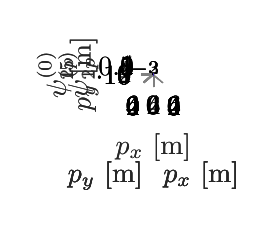
\begin{tikzpicture}

\begin{axis}[%
width=0.34\figurewidth,
height=0.7\figureheight,
at={(0\figurewidth,2\figureheight)},
scale only axis,
xmin=0,
xmax=6,
tick align=outside,
xlabel style={font=\color{white!15!black}},
xlabel={$p_x$~[m]},
ymin=0,
ymax=6,
ylabel style={font=\color{white!15!black}},
ylabel={$p_y$~[m]},
zmin=0,
zmax=0.001,
zlabel style={font=\color{white!15!black}},
zlabel={$\psi_{1\bm p}^{\text{(0)}}$},
view={-45}{25},
axis background/.style={fill=white},
axis x line*=bottom,
axis y line*=left,
axis z line*=left,
xmajorgrids,
ymajorgrids,
zmajorgrids
]

\addplot3[%
surf,
shader=interp, colormap={mymap}{[1pt] rgb(0pt)=(0.2422,0.1504,0.6603); rgb(1pt)=(0.25039,0.164995,0.707614); rgb(2pt)=(0.257771,0.181781,0.751138); rgb(3pt)=(0.264729,0.197757,0.795214); rgb(4pt)=(0.270648,0.214676,0.836371); rgb(5pt)=(0.275114,0.234238,0.870986); rgb(6pt)=(0.2783,0.255871,0.899071); rgb(7pt)=(0.280333,0.278233,0.9221); rgb(8pt)=(0.281338,0.300595,0.941376); rgb(9pt)=(0.281014,0.322757,0.957886); rgb(10pt)=(0.279467,0.344671,0.971676); rgb(11pt)=(0.275971,0.366681,0.982905); rgb(12pt)=(0.269914,0.3892,0.9906); rgb(13pt)=(0.260243,0.412329,0.995157); rgb(14pt)=(0.244033,0.435833,0.998833); rgb(15pt)=(0.220643,0.460257,0.997286); rgb(16pt)=(0.196333,0.484719,0.989152); rgb(17pt)=(0.183405,0.507371,0.979795); rgb(18pt)=(0.178643,0.528857,0.968157); rgb(19pt)=(0.176438,0.549905,0.952019); rgb(20pt)=(0.168743,0.570262,0.935871); rgb(21pt)=(0.154,0.5902,0.9218); rgb(22pt)=(0.146029,0.609119,0.907857); rgb(23pt)=(0.138024,0.627629,0.89729); rgb(24pt)=(0.124814,0.645929,0.888343); rgb(25pt)=(0.111252,0.6635,0.876314); rgb(26pt)=(0.0952095,0.679829,0.859781); rgb(27pt)=(0.0688714,0.694771,0.839357); rgb(28pt)=(0.0296667,0.708167,0.816333); rgb(29pt)=(0.00357143,0.720267,0.7917); rgb(30pt)=(0.00665714,0.731214,0.766014); rgb(31pt)=(0.0433286,0.741095,0.73941); rgb(32pt)=(0.0963952,0.75,0.712038); rgb(33pt)=(0.140771,0.7584,0.684157); rgb(34pt)=(0.1717,0.766962,0.655443); rgb(35pt)=(0.193767,0.775767,0.6251); rgb(36pt)=(0.216086,0.7843,0.5923); rgb(37pt)=(0.246957,0.791795,0.556743); rgb(38pt)=(0.290614,0.79729,0.518829); rgb(39pt)=(0.340643,0.8008,0.478857); rgb(40pt)=(0.3909,0.802871,0.435448); rgb(41pt)=(0.445629,0.802419,0.390919); rgb(42pt)=(0.5044,0.7993,0.348); rgb(43pt)=(0.561562,0.794233,0.304481); rgb(44pt)=(0.617395,0.787619,0.261238); rgb(45pt)=(0.671986,0.779271,0.2227); rgb(46pt)=(0.7242,0.769843,0.191029); rgb(47pt)=(0.773833,0.759805,0.16461); rgb(48pt)=(0.820314,0.749814,0.153529); rgb(49pt)=(0.863433,0.7406,0.159633); rgb(50pt)=(0.903543,0.733029,0.177414); rgb(51pt)=(0.939257,0.728786,0.209957); rgb(52pt)=(0.972757,0.729771,0.239443); rgb(53pt)=(0.995648,0.743371,0.237148); rgb(54pt)=(0.996986,0.765857,0.219943); rgb(55pt)=(0.995205,0.789252,0.202762); rgb(56pt)=(0.9892,0.813567,0.188533); rgb(57pt)=(0.978629,0.838629,0.176557); rgb(58pt)=(0.967648,0.8639,0.16429); rgb(59pt)=(0.96101,0.889019,0.153676); rgb(60pt)=(0.959671,0.913457,0.142257); rgb(61pt)=(0.962795,0.937338,0.12651); rgb(62pt)=(0.969114,0.960629,0.106362); rgb(63pt)=(0.9769,0.9839,0.0805)}, mesh/rows=61]
table[row sep=crcr, point meta=\thisrow{c}] {%
%
x	y	z	c\\
0	0	0.000546448087431694	0.000546448087431694\\
0	0.1	0.000546448087431694	0.000546448087431694\\
0	0.2	0.000546448087431694	0.000546448087431694\\
0	0.3	0.000546448087431694	0.000546448087431694\\
0	0.4	0.000546448087431694	0.000546448087431694\\
0	0.5	0.000546448087431694	0.000546448087431694\\
0	0.6	0.000546448087431694	0.000546448087431694\\
0	0.7	0.000546448087431694	0.000546448087431694\\
0	0.8	0.000546448087431694	0.000546448087431694\\
0	0.9	0.000546448087431694	0.000546448087431694\\
0	1	0.000546448087431694	0.000546448087431694\\
0	1.1	0.000546448087431694	0.000546448087431694\\
0	1.2	0.000546448087431694	0.000546448087431694\\
0	1.3	0.000546448087431694	0.000546448087431694\\
0	1.4	0.000546448087431694	0.000546448087431694\\
0	1.5	0.000546448087431694	0.000546448087431694\\
0	1.6	0.000546448087431694	0.000546448087431694\\
0	1.7	0.000546448087431694	0.000546448087431694\\
0	1.8	0.000546448087431694	0.000546448087431694\\
0	1.9	0.000546448087431694	0.000546448087431694\\
0	2	0.000546448087431694	0.000546448087431694\\
0	2.1	0.000546448087431694	0.000546448087431694\\
0	2.2	0.000546448087431694	0.000546448087431694\\
0	2.3	0.000546448087431694	0.000546448087431694\\
0	2.4	0.000546448087431694	0.000546448087431694\\
0	2.5	0.000546448087431694	0.000546448087431694\\
0	2.6	0.000546448087431694	0.000546448087431694\\
0	2.7	0.000546448087431694	0.000546448087431694\\
0	2.8	0.000546448087431694	0.000546448087431694\\
0	2.9	0.000546448087431694	0.000546448087431694\\
0	3	0.000546448087431694	0.000546448087431694\\
0	3.1	0.000546448087431694	0.000546448087431694\\
0	3.2	0.000546448087431694	0.000546448087431694\\
0	3.3	0.000546448087431694	0.000546448087431694\\
0	3.4	0.000546448087431694	0.000546448087431694\\
0	3.5	0.000546448087431694	0.000546448087431694\\
0	3.6	0.000546448087431694	0.000546448087431694\\
0	3.7	0.000546448087431694	0.000546448087431694\\
0	3.8	0.000546448087431694	0.000546448087431694\\
0	3.9	0.000546448087431694	0.000546448087431694\\
0	4	0.000546448087431694	0.000546448087431694\\
0	4.1	0.000546448087431694	0.000546448087431694\\
0	4.2	0.000546448087431694	0.000546448087431694\\
0	4.3	0.000546448087431694	0.000546448087431694\\
0	4.4	0.000546448087431694	0.000546448087431694\\
0	4.5	0.000546448087431694	0.000546448087431694\\
0	4.6	0.000546448087431694	0.000546448087431694\\
0	4.7	0.000546448087431694	0.000546448087431694\\
0	4.8	0.000546448087431694	0.000546448087431694\\
0	4.9	0.000546448087431694	0.000546448087431694\\
0	5	0.000546448087431694	0.000546448087431694\\
0	5.1	0.000546448087431694	0.000546448087431694\\
0	5.2	0.000546448087431694	0.000546448087431694\\
0	5.3	0.000546448087431694	0.000546448087431694\\
0	5.4	0.000546448087431694	0.000546448087431694\\
0	5.5	0.000546448087431694	0.000546448087431694\\
0	5.6	0.000546448087431694	0.000546448087431694\\
0	5.7	0.000546448087431694	0.000546448087431694\\
0	5.8	0.000546448087431694	0.000546448087431694\\
0	5.9	0.000546448087431694	0.000546448087431694\\
0	6	0.000546448087431694	0.000546448087431694\\
0.1	0	0.000546448087431694	0.000546448087431694\\
0.1	0.1	0.000546448087431694	0.000546448087431694\\
0.1	0.2	0.000546448087431694	0.000546448087431694\\
0.1	0.3	0.000546448087431694	0.000546448087431694\\
0.1	0.4	0.000546448087431694	0.000546448087431694\\
0.1	0.5	0.000546448087431694	0.000546448087431694\\
0.1	0.6	0.000546448087431694	0.000546448087431694\\
0.1	0.7	0.000546448087431694	0.000546448087431694\\
0.1	0.8	0.000546448087431694	0.000546448087431694\\
0.1	0.9	0.000546448087431694	0.000546448087431694\\
0.1	1	0.000546448087431694	0.000546448087431694\\
0.1	1.1	0.000546448087431694	0.000546448087431694\\
0.1	1.2	0.000546448087431694	0.000546448087431694\\
0.1	1.3	0.000546448087431694	0.000546448087431694\\
0.1	1.4	0.000546448087431694	0.000546448087431694\\
0.1	1.5	0.000546448087431694	0.000546448087431694\\
0.1	1.6	0.000546448087431694	0.000546448087431694\\
0.1	1.7	0.000546448087431694	0.000546448087431694\\
0.1	1.8	0.000546448087431694	0.000546448087431694\\
0.1	1.9	0.000546448087431694	0.000546448087431694\\
0.1	2	0.000546448087431694	0.000546448087431694\\
0.1	2.1	0.000546448087431694	0.000546448087431694\\
0.1	2.2	0.000546448087431694	0.000546448087431694\\
0.1	2.3	0.000546448087431694	0.000546448087431694\\
0.1	2.4	0.000546448087431694	0.000546448087431694\\
0.1	2.5	0.000546448087431694	0.000546448087431694\\
0.1	2.6	0.000546448087431694	0.000546448087431694\\
0.1	2.7	0.000546448087431694	0.000546448087431694\\
0.1	2.8	0.000546448087431694	0.000546448087431694\\
0.1	2.9	0.000546448087431694	0.000546448087431694\\
0.1	3	0.000546448087431694	0.000546448087431694\\
0.1	3.1	0.000546448087431694	0.000546448087431694\\
0.1	3.2	0.000546448087431694	0.000546448087431694\\
0.1	3.3	0.000546448087431694	0.000546448087431694\\
0.1	3.4	0.000546448087431694	0.000546448087431694\\
0.1	3.5	0.000546448087431694	0.000546448087431694\\
0.1	3.6	0.000546448087431694	0.000546448087431694\\
0.1	3.7	0.000546448087431694	0.000546448087431694\\
0.1	3.8	0.000546448087431694	0.000546448087431694\\
0.1	3.9	0.000546448087431694	0.000546448087431694\\
0.1	4	0.000546448087431694	0.000546448087431694\\
0.1	4.1	0.000546448087431694	0.000546448087431694\\
0.1	4.2	0.000546448087431694	0.000546448087431694\\
0.1	4.3	0.000546448087431694	0.000546448087431694\\
0.1	4.4	0.000546448087431694	0.000546448087431694\\
0.1	4.5	0.000546448087431694	0.000546448087431694\\
0.1	4.6	0.000546448087431694	0.000546448087431694\\
0.1	4.7	0.000546448087431694	0.000546448087431694\\
0.1	4.8	0.000546448087431694	0.000546448087431694\\
0.1	4.9	0.000546448087431694	0.000546448087431694\\
0.1	5	0.000546448087431694	0.000546448087431694\\
0.1	5.1	0.000546448087431694	0.000546448087431694\\
0.1	5.2	0.000546448087431694	0.000546448087431694\\
0.1	5.3	0.000546448087431694	0.000546448087431694\\
0.1	5.4	0.000546448087431694	0.000546448087431694\\
0.1	5.5	0.000546448087431694	0.000546448087431694\\
0.1	5.6	0.000546448087431694	0.000546448087431694\\
0.1	5.7	0.000546448087431694	0.000546448087431694\\
0.1	5.8	0.000546448087431694	0.000546448087431694\\
0.1	5.9	0.000546448087431694	0.000546448087431694\\
0.1	6	0.000546448087431694	0.000546448087431694\\
0.2	0	0.000546448087431694	0.000546448087431694\\
0.2	0.1	0.000546448087431694	0.000546448087431694\\
0.2	0.2	0.000546448087431694	0.000546448087431694\\
0.2	0.3	0.000546448087431694	0.000546448087431694\\
0.2	0.4	0.000546448087431694	0.000546448087431694\\
0.2	0.5	0.000546448087431694	0.000546448087431694\\
0.2	0.6	0.000546448087431694	0.000546448087431694\\
0.2	0.7	0.000546448087431694	0.000546448087431694\\
0.2	0.8	0.000546448087431694	0.000546448087431694\\
0.2	0.9	0.000546448087431694	0.000546448087431694\\
0.2	1	0.000546448087431694	0.000546448087431694\\
0.2	1.1	0.000546448087431694	0.000546448087431694\\
0.2	1.2	0.000546448087431694	0.000546448087431694\\
0.2	1.3	0.000546448087431694	0.000546448087431694\\
0.2	1.4	0.000546448087431694	0.000546448087431694\\
0.2	1.5	0.000546448087431694	0.000546448087431694\\
0.2	1.6	0.000546448087431694	0.000546448087431694\\
0.2	1.7	0.000546448087431694	0.000546448087431694\\
0.2	1.8	0.000546448087431694	0.000546448087431694\\
0.2	1.9	0.000546448087431694	0.000546448087431694\\
0.2	2	0.000546448087431694	0.000546448087431694\\
0.2	2.1	0.000546448087431694	0.000546448087431694\\
0.2	2.2	0.000546448087431694	0.000546448087431694\\
0.2	2.3	0.000546448087431694	0.000546448087431694\\
0.2	2.4	0.000546448087431694	0.000546448087431694\\
0.2	2.5	0.000546448087431694	0.000546448087431694\\
0.2	2.6	0.000546448087431694	0.000546448087431694\\
0.2	2.7	0.000546448087431694	0.000546448087431694\\
0.2	2.8	0.000546448087431694	0.000546448087431694\\
0.2	2.9	0.000546448087431694	0.000546448087431694\\
0.2	3	0.000546448087431694	0.000546448087431694\\
0.2	3.1	0.000546448087431694	0.000546448087431694\\
0.2	3.2	0.000546448087431694	0.000546448087431694\\
0.2	3.3	0.000546448087431694	0.000546448087431694\\
0.2	3.4	0.000546448087431694	0.000546448087431694\\
0.2	3.5	0.000546448087431694	0.000546448087431694\\
0.2	3.6	0.000546448087431694	0.000546448087431694\\
0.2	3.7	0.000546448087431694	0.000546448087431694\\
0.2	3.8	0.000546448087431694	0.000546448087431694\\
0.2	3.9	0.000546448087431694	0.000546448087431694\\
0.2	4	0.000546448087431694	0.000546448087431694\\
0.2	4.1	0.000546448087431694	0.000546448087431694\\
0.2	4.2	0.000546448087431694	0.000546448087431694\\
0.2	4.3	0.000546448087431694	0.000546448087431694\\
0.2	4.4	0.000546448087431694	0.000546448087431694\\
0.2	4.5	0.000546448087431694	0.000546448087431694\\
0.2	4.6	0.000546448087431694	0.000546448087431694\\
0.2	4.7	0.000546448087431694	0.000546448087431694\\
0.2	4.8	0.000546448087431694	0.000546448087431694\\
0.2	4.9	0.000546448087431694	0.000546448087431694\\
0.2	5	0.000546448087431694	0.000546448087431694\\
0.2	5.1	0.000546448087431694	0.000546448087431694\\
0.2	5.2	0.000546448087431694	0.000546448087431694\\
0.2	5.3	0.000546448087431694	0.000546448087431694\\
0.2	5.4	0.000546448087431694	0.000546448087431694\\
0.2	5.5	0.000546448087431694	0.000546448087431694\\
0.2	5.6	0.000546448087431694	0.000546448087431694\\
0.2	5.7	0.000546448087431694	0.000546448087431694\\
0.2	5.8	0.000546448087431694	0.000546448087431694\\
0.2	5.9	0.000546448087431694	0.000546448087431694\\
0.2	6	0.000546448087431694	0.000546448087431694\\
0.3	0	0.000546448087431694	0.000546448087431694\\
0.3	0.1	0.000546448087431694	0.000546448087431694\\
0.3	0.2	0.000546448087431694	0.000546448087431694\\
0.3	0.3	0.000546448087431694	0.000546448087431694\\
0.3	0.4	0.000546448087431694	0.000546448087431694\\
0.3	0.5	0.000546448087431694	0.000546448087431694\\
0.3	0.6	0.000546448087431694	0.000546448087431694\\
0.3	0.7	0.000546448087431694	0.000546448087431694\\
0.3	0.8	0.000546448087431694	0.000546448087431694\\
0.3	0.9	0.000546448087431694	0.000546448087431694\\
0.3	1	0.000546448087431694	0.000546448087431694\\
0.3	1.1	0.000546448087431694	0.000546448087431694\\
0.3	1.2	0.000546448087431694	0.000546448087431694\\
0.3	1.3	0.000546448087431694	0.000546448087431694\\
0.3	1.4	0.000546448087431694	0.000546448087431694\\
0.3	1.5	0.000546448087431694	0.000546448087431694\\
0.3	1.6	0.000546448087431694	0.000546448087431694\\
0.3	1.7	0.000546448087431694	0.000546448087431694\\
0.3	1.8	0.000546448087431694	0.000546448087431694\\
0.3	1.9	0.000546448087431694	0.000546448087431694\\
0.3	2	0.000546448087431694	0.000546448087431694\\
0.3	2.1	0.000546448087431694	0.000546448087431694\\
0.3	2.2	0.000546448087431694	0.000546448087431694\\
0.3	2.3	0.000546448087431694	0.000546448087431694\\
0.3	2.4	0.000546448087431694	0.000546448087431694\\
0.3	2.5	0.000546448087431694	0.000546448087431694\\
0.3	2.6	0.000546448087431694	0.000546448087431694\\
0.3	2.7	0.000546448087431694	0.000546448087431694\\
0.3	2.8	0.000546448087431694	0.000546448087431694\\
0.3	2.9	0.000546448087431694	0.000546448087431694\\
0.3	3	0.000546448087431694	0.000546448087431694\\
0.3	3.1	0.000546448087431694	0.000546448087431694\\
0.3	3.2	0.000546448087431694	0.000546448087431694\\
0.3	3.3	0.000546448087431694	0.000546448087431694\\
0.3	3.4	0.000546448087431694	0.000546448087431694\\
0.3	3.5	0.000546448087431694	0.000546448087431694\\
0.3	3.6	0.000546448087431694	0.000546448087431694\\
0.3	3.7	0.000546448087431694	0.000546448087431694\\
0.3	3.8	0.000546448087431694	0.000546448087431694\\
0.3	3.9	0.000546448087431694	0.000546448087431694\\
0.3	4	0.000546448087431694	0.000546448087431694\\
0.3	4.1	0.000546448087431694	0.000546448087431694\\
0.3	4.2	0.000546448087431694	0.000546448087431694\\
0.3	4.3	0.000546448087431694	0.000546448087431694\\
0.3	4.4	0.000546448087431694	0.000546448087431694\\
0.3	4.5	0.000546448087431694	0.000546448087431694\\
0.3	4.6	0.000546448087431694	0.000546448087431694\\
0.3	4.7	0.000546448087431694	0.000546448087431694\\
0.3	4.8	0.000546448087431694	0.000546448087431694\\
0.3	4.9	0.000546448087431694	0.000546448087431694\\
0.3	5	0.000546448087431694	0.000546448087431694\\
0.3	5.1	0.000546448087431694	0.000546448087431694\\
0.3	5.2	0.000546448087431694	0.000546448087431694\\
0.3	5.3	0.000546448087431694	0.000546448087431694\\
0.3	5.4	0.000546448087431694	0.000546448087431694\\
0.3	5.5	0.000546448087431694	0.000546448087431694\\
0.3	5.6	0.000546448087431694	0.000546448087431694\\
0.3	5.7	0.000546448087431694	0.000546448087431694\\
0.3	5.8	0.000546448087431694	0.000546448087431694\\
0.3	5.9	0.000546448087431694	0.000546448087431694\\
0.3	6	0.000546448087431694	0.000546448087431694\\
0.4	0	0.000546448087431694	0.000546448087431694\\
0.4	0.1	0.000546448087431694	0.000546448087431694\\
0.4	0.2	0.000546448087431694	0.000546448087431694\\
0.4	0.3	0.000546448087431694	0.000546448087431694\\
0.4	0.4	0.000546448087431694	0.000546448087431694\\
0.4	0.5	0.000546448087431694	0.000546448087431694\\
0.4	0.6	0.000546448087431694	0.000546448087431694\\
0.4	0.7	0.000546448087431694	0.000546448087431694\\
0.4	0.8	0.000546448087431694	0.000546448087431694\\
0.4	0.9	0.000546448087431694	0.000546448087431694\\
0.4	1	0.000546448087431694	0.000546448087431694\\
0.4	1.1	0.000546448087431694	0.000546448087431694\\
0.4	1.2	0.000546448087431694	0.000546448087431694\\
0.4	1.3	0.000546448087431694	0.000546448087431694\\
0.4	1.4	0.000546448087431694	0.000546448087431694\\
0.4	1.5	0.000546448087431694	0.000546448087431694\\
0.4	1.6	0.000546448087431694	0.000546448087431694\\
0.4	1.7	0.000546448087431694	0.000546448087431694\\
0.4	1.8	0.000546448087431694	0.000546448087431694\\
0.4	1.9	0.000546448087431694	0.000546448087431694\\
0.4	2	0.000546448087431694	0.000546448087431694\\
0.4	2.1	0.000546448087431694	0.000546448087431694\\
0.4	2.2	0.000546448087431694	0.000546448087431694\\
0.4	2.3	0.000546448087431694	0.000546448087431694\\
0.4	2.4	0.000546448087431694	0.000546448087431694\\
0.4	2.5	0.000546448087431694	0.000546448087431694\\
0.4	2.6	0.000546448087431694	0.000546448087431694\\
0.4	2.7	0.000546448087431694	0.000546448087431694\\
0.4	2.8	0.000546448087431694	0.000546448087431694\\
0.4	2.9	0.000546448087431694	0.000546448087431694\\
0.4	3	0.000546448087431694	0.000546448087431694\\
0.4	3.1	0.000546448087431694	0.000546448087431694\\
0.4	3.2	0.000546448087431694	0.000546448087431694\\
0.4	3.3	0.000546448087431694	0.000546448087431694\\
0.4	3.4	0.000546448087431694	0.000546448087431694\\
0.4	3.5	0.000546448087431694	0.000546448087431694\\
0.4	3.6	0.000546448087431694	0.000546448087431694\\
0.4	3.7	0.000546448087431694	0.000546448087431694\\
0.4	3.8	0.000546448087431694	0.000546448087431694\\
0.4	3.9	0.000546448087431694	0.000546448087431694\\
0.4	4	0.000546448087431694	0.000546448087431694\\
0.4	4.1	0.000546448087431694	0.000546448087431694\\
0.4	4.2	0.000546448087431694	0.000546448087431694\\
0.4	4.3	0.000546448087431694	0.000546448087431694\\
0.4	4.4	0.000546448087431694	0.000546448087431694\\
0.4	4.5	0.000546448087431694	0.000546448087431694\\
0.4	4.6	0.000546448087431694	0.000546448087431694\\
0.4	4.7	0.000546448087431694	0.000546448087431694\\
0.4	4.8	0.000546448087431694	0.000546448087431694\\
0.4	4.9	0.000546448087431694	0.000546448087431694\\
0.4	5	0.000546448087431694	0.000546448087431694\\
0.4	5.1	0.000546448087431694	0.000546448087431694\\
0.4	5.2	0.000546448087431694	0.000546448087431694\\
0.4	5.3	0.000546448087431694	0.000546448087431694\\
0.4	5.4	0.000546448087431694	0.000546448087431694\\
0.4	5.5	0.000546448087431694	0.000546448087431694\\
0.4	5.6	0.000546448087431694	0.000546448087431694\\
0.4	5.7	0.000546448087431694	0.000546448087431694\\
0.4	5.8	0.000546448087431694	0.000546448087431694\\
0.4	5.9	0.000546448087431694	0.000546448087431694\\
0.4	6	0.000546448087431694	0.000546448087431694\\
0.5	0	0.000546448087431694	0.000546448087431694\\
0.5	0.1	0.000546448087431694	0.000546448087431694\\
0.5	0.2	0.000546448087431694	0.000546448087431694\\
0.5	0.3	0.000546448087431694	0.000546448087431694\\
0.5	0.4	0.000546448087431694	0.000546448087431694\\
0.5	0.5	0.000546448087431694	0.000546448087431694\\
0.5	0.6	0.000546448087431694	0.000546448087431694\\
0.5	0.7	0.000546448087431694	0.000546448087431694\\
0.5	0.8	0.000546448087431694	0.000546448087431694\\
0.5	0.9	0.000546448087431694	0.000546448087431694\\
0.5	1	0.000546448087431694	0.000546448087431694\\
0.5	1.1	0.000546448087431694	0.000546448087431694\\
0.5	1.2	0.000546448087431694	0.000546448087431694\\
0.5	1.3	0.000546448087431694	0.000546448087431694\\
0.5	1.4	0.000546448087431694	0.000546448087431694\\
0.5	1.5	0.000546448087431694	0.000546448087431694\\
0.5	1.6	0.000546448087431694	0.000546448087431694\\
0.5	1.7	0.000546448087431694	0.000546448087431694\\
0.5	1.8	0.000546448087431694	0.000546448087431694\\
0.5	1.9	0.000546448087431694	0.000546448087431694\\
0.5	2	0.000546448087431694	0.000546448087431694\\
0.5	2.1	0.000546448087431694	0.000546448087431694\\
0.5	2.2	0.000546448087431694	0.000546448087431694\\
0.5	2.3	0.000546448087431694	0.000546448087431694\\
0.5	2.4	0.000546448087431694	0.000546448087431694\\
0.5	2.5	0.000546448087431694	0.000546448087431694\\
0.5	2.6	0.000546448087431694	0.000546448087431694\\
0.5	2.7	0.000546448087431694	0.000546448087431694\\
0.5	2.8	0.000546448087431694	0.000546448087431694\\
0.5	2.9	0.000546448087431694	0.000546448087431694\\
0.5	3	0.000546448087431694	0.000546448087431694\\
0.5	3.1	0.000546448087431694	0.000546448087431694\\
0.5	3.2	0.000546448087431694	0.000546448087431694\\
0.5	3.3	0.000546448087431694	0.000546448087431694\\
0.5	3.4	0.000546448087431694	0.000546448087431694\\
0.5	3.5	0.000546448087431694	0.000546448087431694\\
0.5	3.6	0.000546448087431694	0.000546448087431694\\
0.5	3.7	0.000546448087431694	0.000546448087431694\\
0.5	3.8	0.000546448087431694	0.000546448087431694\\
0.5	3.9	0.000546448087431694	0.000546448087431694\\
0.5	4	0.000546448087431694	0.000546448087431694\\
0.5	4.1	0.000546448087431694	0.000546448087431694\\
0.5	4.2	0.000546448087431694	0.000546448087431694\\
0.5	4.3	0.000546448087431694	0.000546448087431694\\
0.5	4.4	0.000546448087431694	0.000546448087431694\\
0.5	4.5	0.000546448087431694	0.000546448087431694\\
0.5	4.6	0.000546448087431694	0.000546448087431694\\
0.5	4.7	0.000546448087431694	0.000546448087431694\\
0.5	4.8	0.000546448087431694	0.000546448087431694\\
0.5	4.9	0.000546448087431694	0.000546448087431694\\
0.5	5	0.000546448087431694	0.000546448087431694\\
0.5	5.1	0.000546448087431694	0.000546448087431694\\
0.5	5.2	0.000546448087431694	0.000546448087431694\\
0.5	5.3	0.000546448087431694	0.000546448087431694\\
0.5	5.4	0.000546448087431694	0.000546448087431694\\
0.5	5.5	0.000546448087431694	0.000546448087431694\\
0.5	5.6	0.000546448087431694	0.000546448087431694\\
0.5	5.7	0.000546448087431694	0.000546448087431694\\
0.5	5.8	0.000546448087431694	0.000546448087431694\\
0.5	5.9	0.000546448087431694	0.000546448087431694\\
0.5	6	0.000546448087431694	0.000546448087431694\\
0.6	0	0.000546448087431694	0.000546448087431694\\
0.6	0.1	0.000546448087431694	0.000546448087431694\\
0.6	0.2	0.000546448087431694	0.000546448087431694\\
0.6	0.3	0.000546448087431694	0.000546448087431694\\
0.6	0.4	0.000546448087431694	0.000546448087431694\\
0.6	0.5	0.000546448087431694	0.000546448087431694\\
0.6	0.6	0.000546448087431694	0.000546448087431694\\
0.6	0.7	0.000546448087431694	0.000546448087431694\\
0.6	0.8	0.000546448087431694	0.000546448087431694\\
0.6	0.9	0.000546448087431694	0.000546448087431694\\
0.6	1	0.000546448087431694	0.000546448087431694\\
0.6	1.1	0.000546448087431694	0.000546448087431694\\
0.6	1.2	0.000546448087431694	0.000546448087431694\\
0.6	1.3	0.000546448087431694	0.000546448087431694\\
0.6	1.4	0.000546448087431694	0.000546448087431694\\
0.6	1.5	0.000546448087431694	0.000546448087431694\\
0.6	1.6	0.000546448087431694	0.000546448087431694\\
0.6	1.7	0.000546448087431694	0.000546448087431694\\
0.6	1.8	0.000546448087431694	0.000546448087431694\\
0.6	1.9	0.000546448087431694	0.000546448087431694\\
0.6	2	0.000546448087431694	0.000546448087431694\\
0.6	2.1	0.000546448087431694	0.000546448087431694\\
0.6	2.2	0.000546448087431694	0.000546448087431694\\
0.6	2.3	0.000546448087431694	0.000546448087431694\\
0.6	2.4	0.000546448087431694	0.000546448087431694\\
0.6	2.5	0.000546448087431694	0.000546448087431694\\
0.6	2.6	0.000546448087431694	0.000546448087431694\\
0.6	2.7	0.000546448087431694	0.000546448087431694\\
0.6	2.8	0.000546448087431694	0.000546448087431694\\
0.6	2.9	0.000546448087431694	0.000546448087431694\\
0.6	3	0.000546448087431694	0.000546448087431694\\
0.6	3.1	0.000546448087431694	0.000546448087431694\\
0.6	3.2	0.000546448087431694	0.000546448087431694\\
0.6	3.3	0.000546448087431694	0.000546448087431694\\
0.6	3.4	0.000546448087431694	0.000546448087431694\\
0.6	3.5	0.000546448087431694	0.000546448087431694\\
0.6	3.6	0.000546448087431694	0.000546448087431694\\
0.6	3.7	0.000546448087431694	0.000546448087431694\\
0.6	3.8	0.000546448087431694	0.000546448087431694\\
0.6	3.9	0.000546448087431694	0.000546448087431694\\
0.6	4	0.000546448087431694	0.000546448087431694\\
0.6	4.1	0.000546448087431694	0.000546448087431694\\
0.6	4.2	0.000546448087431694	0.000546448087431694\\
0.6	4.3	0.000546448087431694	0.000546448087431694\\
0.6	4.4	0.000546448087431694	0.000546448087431694\\
0.6	4.5	0.000546448087431694	0.000546448087431694\\
0.6	4.6	0.000546448087431694	0.000546448087431694\\
0.6	4.7	0.000546448087431694	0.000546448087431694\\
0.6	4.8	0.000546448087431694	0.000546448087431694\\
0.6	4.9	0.000546448087431694	0.000546448087431694\\
0.6	5	0.000546448087431694	0.000546448087431694\\
0.6	5.1	0.000546448087431694	0.000546448087431694\\
0.6	5.2	0.000546448087431694	0.000546448087431694\\
0.6	5.3	0.000546448087431694	0.000546448087431694\\
0.6	5.4	0.000546448087431694	0.000546448087431694\\
0.6	5.5	0.000546448087431694	0.000546448087431694\\
0.6	5.6	0.000546448087431694	0.000546448087431694\\
0.6	5.7	0.000546448087431694	0.000546448087431694\\
0.6	5.8	0.000546448087431694	0.000546448087431694\\
0.6	5.9	0.000546448087431694	0.000546448087431694\\
0.6	6	0.000546448087431694	0.000546448087431694\\
0.7	0	0.000546448087431694	0.000546448087431694\\
0.7	0.1	0.000546448087431694	0.000546448087431694\\
0.7	0.2	0.000546448087431694	0.000546448087431694\\
0.7	0.3	0.000546448087431694	0.000546448087431694\\
0.7	0.4	0.000546448087431694	0.000546448087431694\\
0.7	0.5	0.000546448087431694	0.000546448087431694\\
0.7	0.6	0.000546448087431694	0.000546448087431694\\
0.7	0.7	0.000546448087431694	0.000546448087431694\\
0.7	0.8	0.000546448087431694	0.000546448087431694\\
0.7	0.9	0.000546448087431694	0.000546448087431694\\
0.7	1	0.000546448087431694	0.000546448087431694\\
0.7	1.1	0.000546448087431694	0.000546448087431694\\
0.7	1.2	0.000546448087431694	0.000546448087431694\\
0.7	1.3	0.000546448087431694	0.000546448087431694\\
0.7	1.4	0.000546448087431694	0.000546448087431694\\
0.7	1.5	0.000546448087431694	0.000546448087431694\\
0.7	1.6	0.000546448087431694	0.000546448087431694\\
0.7	1.7	0.000546448087431694	0.000546448087431694\\
0.7	1.8	0.000546448087431694	0.000546448087431694\\
0.7	1.9	0.000546448087431694	0.000546448087431694\\
0.7	2	0.000546448087431694	0.000546448087431694\\
0.7	2.1	0.000546448087431694	0.000546448087431694\\
0.7	2.2	0.000546448087431694	0.000546448087431694\\
0.7	2.3	0.000546448087431694	0.000546448087431694\\
0.7	2.4	0.000546448087431694	0.000546448087431694\\
0.7	2.5	0.000546448087431694	0.000546448087431694\\
0.7	2.6	0.000546448087431694	0.000546448087431694\\
0.7	2.7	0.000546448087431694	0.000546448087431694\\
0.7	2.8	0.000546448087431694	0.000546448087431694\\
0.7	2.9	0.000546448087431694	0.000546448087431694\\
0.7	3	0.000546448087431694	0.000546448087431694\\
0.7	3.1	0.000546448087431694	0.000546448087431694\\
0.7	3.2	0.000546448087431694	0.000546448087431694\\
0.7	3.3	0.000546448087431694	0.000546448087431694\\
0.7	3.4	0.000546448087431694	0.000546448087431694\\
0.7	3.5	0.000546448087431694	0.000546448087431694\\
0.7	3.6	0.000546448087431694	0.000546448087431694\\
0.7	3.7	0.000546448087431694	0.000546448087431694\\
0.7	3.8	0.000546448087431694	0.000546448087431694\\
0.7	3.9	0.000546448087431694	0.000546448087431694\\
0.7	4	0.000546448087431694	0.000546448087431694\\
0.7	4.1	0.000546448087431694	0.000546448087431694\\
0.7	4.2	0.000546448087431694	0.000546448087431694\\
0.7	4.3	0.000546448087431694	0.000546448087431694\\
0.7	4.4	0.000546448087431694	0.000546448087431694\\
0.7	4.5	0.000546448087431694	0.000546448087431694\\
0.7	4.6	0.000546448087431694	0.000546448087431694\\
0.7	4.7	0.000546448087431694	0.000546448087431694\\
0.7	4.8	0.000546448087431694	0.000546448087431694\\
0.7	4.9	0.000546448087431694	0.000546448087431694\\
0.7	5	0.000546448087431694	0.000546448087431694\\
0.7	5.1	0.000546448087431694	0.000546448087431694\\
0.7	5.2	0.000546448087431694	0.000546448087431694\\
0.7	5.3	0.000546448087431694	0.000546448087431694\\
0.7	5.4	0.000546448087431694	0.000546448087431694\\
0.7	5.5	0.000546448087431694	0.000546448087431694\\
0.7	5.6	0.000546448087431694	0.000546448087431694\\
0.7	5.7	0.000546448087431694	0.000546448087431694\\
0.7	5.8	0.000546448087431694	0.000546448087431694\\
0.7	5.9	0.000546448087431694	0.000546448087431694\\
0.7	6	0.000546448087431694	0.000546448087431694\\
0.8	0	0.000546448087431694	0.000546448087431694\\
0.8	0.1	0.000546448087431694	0.000546448087431694\\
0.8	0.2	0.000546448087431694	0.000546448087431694\\
0.8	0.3	0.000546448087431694	0.000546448087431694\\
0.8	0.4	0.000546448087431694	0.000546448087431694\\
0.8	0.5	0.000546448087431694	0.000546448087431694\\
0.8	0.6	0.000546448087431694	0.000546448087431694\\
0.8	0.7	0.000546448087431694	0.000546448087431694\\
0.8	0.8	0.000546448087431694	0.000546448087431694\\
0.8	0.9	0.000546448087431694	0.000546448087431694\\
0.8	1	0.000546448087431694	0.000546448087431694\\
0.8	1.1	0.000546448087431694	0.000546448087431694\\
0.8	1.2	0.000546448087431694	0.000546448087431694\\
0.8	1.3	0.000546448087431694	0.000546448087431694\\
0.8	1.4	0.000546448087431694	0.000546448087431694\\
0.8	1.5	0.000546448087431694	0.000546448087431694\\
0.8	1.6	0.000546448087431694	0.000546448087431694\\
0.8	1.7	0.000546448087431694	0.000546448087431694\\
0.8	1.8	0.000546448087431694	0.000546448087431694\\
0.8	1.9	0.000546448087431694	0.000546448087431694\\
0.8	2	0.000546448087431694	0.000546448087431694\\
0.8	2.1	0.000546448087431694	0.000546448087431694\\
0.8	2.2	0.000546448087431694	0.000546448087431694\\
0.8	2.3	0.000546448087431694	0.000546448087431694\\
0.8	2.4	0.000546448087431694	0.000546448087431694\\
0.8	2.5	0.000546448087431694	0.000546448087431694\\
0.8	2.6	0.000546448087431694	0.000546448087431694\\
0.8	2.7	0.000546448087431694	0.000546448087431694\\
0.8	2.8	0.000546448087431694	0.000546448087431694\\
0.8	2.9	0.000546448087431694	0.000546448087431694\\
0.8	3	0.000546448087431694	0.000546448087431694\\
0.8	3.1	0.000546448087431694	0.000546448087431694\\
0.8	3.2	0.000546448087431694	0.000546448087431694\\
0.8	3.3	0.000546448087431694	0.000546448087431694\\
0.8	3.4	0.000546448087431694	0.000546448087431694\\
0.8	3.5	0.000546448087431694	0.000546448087431694\\
0.8	3.6	0.000546448087431694	0.000546448087431694\\
0.8	3.7	0.000546448087431694	0.000546448087431694\\
0.8	3.8	0.000546448087431694	0.000546448087431694\\
0.8	3.9	0.000546448087431694	0.000546448087431694\\
0.8	4	0.000546448087431694	0.000546448087431694\\
0.8	4.1	0.000546448087431694	0.000546448087431694\\
0.8	4.2	0.000546448087431694	0.000546448087431694\\
0.8	4.3	0.000546448087431694	0.000546448087431694\\
0.8	4.4	0.000546448087431694	0.000546448087431694\\
0.8	4.5	0.000546448087431694	0.000546448087431694\\
0.8	4.6	0.000546448087431694	0.000546448087431694\\
0.8	4.7	0.000546448087431694	0.000546448087431694\\
0.8	4.8	0.000546448087431694	0.000546448087431694\\
0.8	4.9	0.000546448087431694	0.000546448087431694\\
0.8	5	0.000546448087431694	0.000546448087431694\\
0.8	5.1	0.000546448087431694	0.000546448087431694\\
0.8	5.2	0.000546448087431694	0.000546448087431694\\
0.8	5.3	0.000546448087431694	0.000546448087431694\\
0.8	5.4	0.000546448087431694	0.000546448087431694\\
0.8	5.5	0.000546448087431694	0.000546448087431694\\
0.8	5.6	0.000546448087431694	0.000546448087431694\\
0.8	5.7	0.000546448087431694	0.000546448087431694\\
0.8	5.8	0.000546448087431694	0.000546448087431694\\
0.8	5.9	0.000546448087431694	0.000546448087431694\\
0.8	6	0.000546448087431694	0.000546448087431694\\
0.9	0	0.000546448087431694	0.000546448087431694\\
0.9	0.1	0.000546448087431694	0.000546448087431694\\
0.9	0.2	0.000546448087431694	0.000546448087431694\\
0.9	0.3	0.000546448087431694	0.000546448087431694\\
0.9	0.4	0.000546448087431694	0.000546448087431694\\
0.9	0.5	0.000546448087431694	0.000546448087431694\\
0.9	0.6	0.000546448087431694	0.000546448087431694\\
0.9	0.7	0.000546448087431694	0.000546448087431694\\
0.9	0.8	0.000546448087431694	0.000546448087431694\\
0.9	0.9	0.000546448087431694	0.000546448087431694\\
0.9	1	0.000546448087431694	0.000546448087431694\\
0.9	1.1	0.000546448087431694	0.000546448087431694\\
0.9	1.2	0.000546448087431694	0.000546448087431694\\
0.9	1.3	0.000546448087431694	0.000546448087431694\\
0.9	1.4	0.000546448087431694	0.000546448087431694\\
0.9	1.5	0.000546448087431694	0.000546448087431694\\
0.9	1.6	0.000546448087431694	0.000546448087431694\\
0.9	1.7	0.000546448087431694	0.000546448087431694\\
0.9	1.8	0.000546448087431694	0.000546448087431694\\
0.9	1.9	0.000546448087431694	0.000546448087431694\\
0.9	2	0.000546448087431694	0.000546448087431694\\
0.9	2.1	0.000546448087431694	0.000546448087431694\\
0.9	2.2	0.000546448087431694	0.000546448087431694\\
0.9	2.3	0.000546448087431694	0.000546448087431694\\
0.9	2.4	0.000546448087431694	0.000546448087431694\\
0.9	2.5	0.000546448087431694	0.000546448087431694\\
0.9	2.6	0.000546448087431694	0.000546448087431694\\
0.9	2.7	0.000546448087431694	0.000546448087431694\\
0.9	2.8	0.000546448087431694	0.000546448087431694\\
0.9	2.9	0.000546448087431694	0.000546448087431694\\
0.9	3	0.000546448087431694	0.000546448087431694\\
0.9	3.1	0.000546448087431694	0.000546448087431694\\
0.9	3.2	0.000546448087431694	0.000546448087431694\\
0.9	3.3	0.000546448087431694	0.000546448087431694\\
0.9	3.4	0.000546448087431694	0.000546448087431694\\
0.9	3.5	0.000546448087431694	0.000546448087431694\\
0.9	3.6	0.000546448087431694	0.000546448087431694\\
0.9	3.7	0.000546448087431694	0.000546448087431694\\
0.9	3.8	0.000546448087431694	0.000546448087431694\\
0.9	3.9	0.000546448087431694	0.000546448087431694\\
0.9	4	0.000546448087431694	0.000546448087431694\\
0.9	4.1	0.000546448087431694	0.000546448087431694\\
0.9	4.2	0.000546448087431694	0.000546448087431694\\
0.9	4.3	0.000546448087431694	0.000546448087431694\\
0.9	4.4	0.000546448087431694	0.000546448087431694\\
0.9	4.5	0.000546448087431694	0.000546448087431694\\
0.9	4.6	0.000546448087431694	0.000546448087431694\\
0.9	4.7	0.000546448087431694	0.000546448087431694\\
0.9	4.8	0.000546448087431694	0.000546448087431694\\
0.9	4.9	0.000546448087431694	0.000546448087431694\\
0.9	5	0.000546448087431694	0.000546448087431694\\
0.9	5.1	0.000546448087431694	0.000546448087431694\\
0.9	5.2	0.000546448087431694	0.000546448087431694\\
0.9	5.3	0.000546448087431694	0.000546448087431694\\
0.9	5.4	0.000546448087431694	0.000546448087431694\\
0.9	5.5	0.000546448087431694	0.000546448087431694\\
0.9	5.6	0.000546448087431694	0.000546448087431694\\
0.9	5.7	0.000546448087431694	0.000546448087431694\\
0.9	5.8	0.000546448087431694	0.000546448087431694\\
0.9	5.9	0.000546448087431694	0.000546448087431694\\
0.9	6	0.000546448087431694	0.000546448087431694\\
1	0	0.000546448087431694	0.000546448087431694\\
1	0.1	0.000546448087431694	0.000546448087431694\\
1	0.2	0.000546448087431694	0.000546448087431694\\
1	0.3	0.000546448087431694	0.000546448087431694\\
1	0.4	0.000546448087431694	0.000546448087431694\\
1	0.5	0.000546448087431694	0.000546448087431694\\
1	0.6	0.000546448087431694	0.000546448087431694\\
1	0.7	0.000546448087431694	0.000546448087431694\\
1	0.8	0.000546448087431694	0.000546448087431694\\
1	0.9	0.000546448087431694	0.000546448087431694\\
1	1	0.000546448087431694	0.000546448087431694\\
1	1.1	0.000546448087431694	0.000546448087431694\\
1	1.2	0.000546448087431694	0.000546448087431694\\
1	1.3	0.000546448087431694	0.000546448087431694\\
1	1.4	0.000546448087431694	0.000546448087431694\\
1	1.5	0.000546448087431694	0.000546448087431694\\
1	1.6	0.000546448087431694	0.000546448087431694\\
1	1.7	0.000546448087431694	0.000546448087431694\\
1	1.8	0.000546448087431694	0.000546448087431694\\
1	1.9	0.000546448087431694	0.000546448087431694\\
1	2	0.000546448087431694	0.000546448087431694\\
1	2.1	0.000546448087431694	0.000546448087431694\\
1	2.2	0.000546448087431694	0.000546448087431694\\
1	2.3	0.000546448087431694	0.000546448087431694\\
1	2.4	0.000546448087431694	0.000546448087431694\\
1	2.5	0.000546448087431694	0.000546448087431694\\
1	2.6	0.000546448087431694	0.000546448087431694\\
1	2.7	0.000546448087431694	0.000546448087431694\\
1	2.8	0.000546448087431694	0.000546448087431694\\
1	2.9	0.000546448087431694	0.000546448087431694\\
1	3	0.000546448087431694	0.000546448087431694\\
1	3.1	0.000546448087431694	0.000546448087431694\\
1	3.2	0.000546448087431694	0.000546448087431694\\
1	3.3	0.000546448087431694	0.000546448087431694\\
1	3.4	0.000546448087431694	0.000546448087431694\\
1	3.5	0.000546448087431694	0.000546448087431694\\
1	3.6	0.000546448087431694	0.000546448087431694\\
1	3.7	0.000546448087431694	0.000546448087431694\\
1	3.8	0.000546448087431694	0.000546448087431694\\
1	3.9	0.000546448087431694	0.000546448087431694\\
1	4	0.000546448087431694	0.000546448087431694\\
1	4.1	0.000546448087431694	0.000546448087431694\\
1	4.2	0.000546448087431694	0.000546448087431694\\
1	4.3	0.000546448087431694	0.000546448087431694\\
1	4.4	0.000546448087431694	0.000546448087431694\\
1	4.5	0.000546448087431694	0.000546448087431694\\
1	4.6	0.000546448087431694	0.000546448087431694\\
1	4.7	0.000546448087431694	0.000546448087431694\\
1	4.8	0.000546448087431694	0.000546448087431694\\
1	4.9	0.000546448087431694	0.000546448087431694\\
1	5	0.000546448087431694	0.000546448087431694\\
1	5.1	0.000546448087431694	0.000546448087431694\\
1	5.2	0.000546448087431694	0.000546448087431694\\
1	5.3	0.000546448087431694	0.000546448087431694\\
1	5.4	0.000546448087431694	0.000546448087431694\\
1	5.5	0.000546448087431694	0.000546448087431694\\
1	5.6	0.000546448087431694	0.000546448087431694\\
1	5.7	0.000546448087431694	0.000546448087431694\\
1	5.8	0.000546448087431694	0.000546448087431694\\
1	5.9	0.000546448087431694	0.000546448087431694\\
1	6	0.000546448087431694	0.000546448087431694\\
1.1	0	0.000546448087431694	0.000546448087431694\\
1.1	0.1	0.000546448087431694	0.000546448087431694\\
1.1	0.2	0.000546448087431694	0.000546448087431694\\
1.1	0.3	0.000546448087431694	0.000546448087431694\\
1.1	0.4	0.000546448087431694	0.000546448087431694\\
1.1	0.5	0.000546448087431694	0.000546448087431694\\
1.1	0.6	0.000546448087431694	0.000546448087431694\\
1.1	0.7	0.000546448087431694	0.000546448087431694\\
1.1	0.8	0.000546448087431694	0.000546448087431694\\
1.1	0.9	0.000546448087431694	0.000546448087431694\\
1.1	1	0.000546448087431694	0.000546448087431694\\
1.1	1.1	0.000546448087431694	0.000546448087431694\\
1.1	1.2	0.000546448087431694	0.000546448087431694\\
1.1	1.3	0.000546448087431694	0.000546448087431694\\
1.1	1.4	0.000546448087431694	0.000546448087431694\\
1.1	1.5	0.000546448087431694	0.000546448087431694\\
1.1	1.6	0.000546448087431694	0.000546448087431694\\
1.1	1.7	0.000546448087431694	0.000546448087431694\\
1.1	1.8	0.000546448087431694	0.000546448087431694\\
1.1	1.9	0.000546448087431694	0.000546448087431694\\
1.1	2	0.000546448087431694	0.000546448087431694\\
1.1	2.1	0.000546448087431694	0.000546448087431694\\
1.1	2.2	0.000546448087431694	0.000546448087431694\\
1.1	2.3	0.000546448087431694	0.000546448087431694\\
1.1	2.4	0.000546448087431694	0.000546448087431694\\
1.1	2.5	0.000546448087431694	0.000546448087431694\\
1.1	2.6	0.000546448087431694	0.000546448087431694\\
1.1	2.7	0.000546448087431694	0.000546448087431694\\
1.1	2.8	0.000546448087431694	0.000546448087431694\\
1.1	2.9	0.000546448087431694	0.000546448087431694\\
1.1	3	0.000546448087431694	0.000546448087431694\\
1.1	3.1	0.000546448087431694	0.000546448087431694\\
1.1	3.2	0.000546448087431694	0.000546448087431694\\
1.1	3.3	0.000546448087431694	0.000546448087431694\\
1.1	3.4	0.000546448087431694	0.000546448087431694\\
1.1	3.5	0.000546448087431694	0.000546448087431694\\
1.1	3.6	0.000546448087431694	0.000546448087431694\\
1.1	3.7	0.000546448087431694	0.000546448087431694\\
1.1	3.8	0.000546448087431694	0.000546448087431694\\
1.1	3.9	0.000546448087431694	0.000546448087431694\\
1.1	4	0.000546448087431694	0.000546448087431694\\
1.1	4.1	0.000546448087431694	0.000546448087431694\\
1.1	4.2	0.000546448087431694	0.000546448087431694\\
1.1	4.3	0.000546448087431694	0.000546448087431694\\
1.1	4.4	0.000546448087431694	0.000546448087431694\\
1.1	4.5	0.000546448087431694	0.000546448087431694\\
1.1	4.6	0.000546448087431694	0.000546448087431694\\
1.1	4.7	0.000546448087431694	0.000546448087431694\\
1.1	4.8	0.000546448087431694	0.000546448087431694\\
1.1	4.9	0.000546448087431694	0.000546448087431694\\
1.1	5	0.000546448087431694	0.000546448087431694\\
1.1	5.1	0.000546448087431694	0.000546448087431694\\
1.1	5.2	0.000546448087431694	0.000546448087431694\\
1.1	5.3	0.000546448087431694	0.000546448087431694\\
1.1	5.4	0.000546448087431694	0.000546448087431694\\
1.1	5.5	0.000546448087431694	0.000546448087431694\\
1.1	5.6	0.000546448087431694	0.000546448087431694\\
1.1	5.7	0.000546448087431694	0.000546448087431694\\
1.1	5.8	0.000546448087431694	0.000546448087431694\\
1.1	5.9	0.000546448087431694	0.000546448087431694\\
1.1	6	0.000546448087431694	0.000546448087431694\\
1.2	0	0.000546448087431694	0.000546448087431694\\
1.2	0.1	0.000546448087431694	0.000546448087431694\\
1.2	0.2	0.000546448087431694	0.000546448087431694\\
1.2	0.3	0.000546448087431694	0.000546448087431694\\
1.2	0.4	0.000546448087431694	0.000546448087431694\\
1.2	0.5	0.000546448087431694	0.000546448087431694\\
1.2	0.6	0.000546448087431694	0.000546448087431694\\
1.2	0.7	0.000546448087431694	0.000546448087431694\\
1.2	0.8	0.000546448087431694	0.000546448087431694\\
1.2	0.9	0.000546448087431694	0.000546448087431694\\
1.2	1	0.000546448087431694	0.000546448087431694\\
1.2	1.1	0.000546448087431694	0.000546448087431694\\
1.2	1.2	0.000546448087431694	0.000546448087431694\\
1.2	1.3	0.000546448087431694	0.000546448087431694\\
1.2	1.4	0.000546448087431694	0.000546448087431694\\
1.2	1.5	0.000546448087431694	0.000546448087431694\\
1.2	1.6	0.000546448087431694	0.000546448087431694\\
1.2	1.7	0.000546448087431694	0.000546448087431694\\
1.2	1.8	0.000546448087431694	0.000546448087431694\\
1.2	1.9	0.000546448087431694	0.000546448087431694\\
1.2	2	0.000546448087431694	0.000546448087431694\\
1.2	2.1	0.000546448087431694	0.000546448087431694\\
1.2	2.2	0.000546448087431694	0.000546448087431694\\
1.2	2.3	0.000546448087431694	0.000546448087431694\\
1.2	2.4	0.000546448087431694	0.000546448087431694\\
1.2	2.5	0.000546448087431694	0.000546448087431694\\
1.2	2.6	0.000546448087431694	0.000546448087431694\\
1.2	2.7	0.000546448087431694	0.000546448087431694\\
1.2	2.8	0.000546448087431694	0.000546448087431694\\
1.2	2.9	0.000546448087431694	0.000546448087431694\\
1.2	3	0.000546448087431694	0.000546448087431694\\
1.2	3.1	0.000546448087431694	0.000546448087431694\\
1.2	3.2	0.000546448087431694	0.000546448087431694\\
1.2	3.3	0.000546448087431694	0.000546448087431694\\
1.2	3.4	0.000546448087431694	0.000546448087431694\\
1.2	3.5	0.000546448087431694	0.000546448087431694\\
1.2	3.6	0.000546448087431694	0.000546448087431694\\
1.2	3.7	0.000546448087431694	0.000546448087431694\\
1.2	3.8	0.000546448087431694	0.000546448087431694\\
1.2	3.9	0.000546448087431694	0.000546448087431694\\
1.2	4	0.000546448087431694	0.000546448087431694\\
1.2	4.1	0.000546448087431694	0.000546448087431694\\
1.2	4.2	0.000546448087431694	0.000546448087431694\\
1.2	4.3	0.000546448087431694	0.000546448087431694\\
1.2	4.4	0.000546448087431694	0.000546448087431694\\
1.2	4.5	0.000546448087431694	0.000546448087431694\\
1.2	4.6	0.000546448087431694	0.000546448087431694\\
1.2	4.7	0.000546448087431694	0.000546448087431694\\
1.2	4.8	0.000546448087431694	0.000546448087431694\\
1.2	4.9	0.000546448087431694	0.000546448087431694\\
1.2	5	0.000546448087431694	0.000546448087431694\\
1.2	5.1	0.000546448087431694	0.000546448087431694\\
1.2	5.2	0.000546448087431694	0.000546448087431694\\
1.2	5.3	0.000546448087431694	0.000546448087431694\\
1.2	5.4	0.000546448087431694	0.000546448087431694\\
1.2	5.5	0.000546448087431694	0.000546448087431694\\
1.2	5.6	0.000546448087431694	0.000546448087431694\\
1.2	5.7	0.000546448087431694	0.000546448087431694\\
1.2	5.8	0.000546448087431694	0.000546448087431694\\
1.2	5.9	0.000546448087431694	0.000546448087431694\\
1.2	6	0.000546448087431694	0.000546448087431694\\
1.3	0	0.000546448087431694	0.000546448087431694\\
1.3	0.1	0.000546448087431694	0.000546448087431694\\
1.3	0.2	0.000546448087431694	0.000546448087431694\\
1.3	0.3	0.000546448087431694	0.000546448087431694\\
1.3	0.4	0.000546448087431694	0.000546448087431694\\
1.3	0.5	0.000546448087431694	0.000546448087431694\\
1.3	0.6	0.000546448087431694	0.000546448087431694\\
1.3	0.7	0.000546448087431694	0.000546448087431694\\
1.3	0.8	0.000546448087431694	0.000546448087431694\\
1.3	0.9	0.000546448087431694	0.000546448087431694\\
1.3	1	0.000546448087431694	0.000546448087431694\\
1.3	1.1	0.000546448087431694	0.000546448087431694\\
1.3	1.2	0.000546448087431694	0.000546448087431694\\
1.3	1.3	0.000546448087431694	0.000546448087431694\\
1.3	1.4	0.000546448087431694	0.000546448087431694\\
1.3	1.5	0.000546448087431694	0.000546448087431694\\
1.3	1.6	0.000546448087431694	0.000546448087431694\\
1.3	1.7	0.000546448087431694	0.000546448087431694\\
1.3	1.8	0.000546448087431694	0.000546448087431694\\
1.3	1.9	0.000546448087431694	0.000546448087431694\\
1.3	2	0.000546448087431694	0.000546448087431694\\
1.3	2.1	0.000546448087431694	0.000546448087431694\\
1.3	2.2	0.000546448087431694	0.000546448087431694\\
1.3	2.3	0.000546448087431694	0.000546448087431694\\
1.3	2.4	0.000546448087431694	0.000546448087431694\\
1.3	2.5	0.000546448087431694	0.000546448087431694\\
1.3	2.6	0.000546448087431694	0.000546448087431694\\
1.3	2.7	0.000546448087431694	0.000546448087431694\\
1.3	2.8	0.000546448087431694	0.000546448087431694\\
1.3	2.9	0.000546448087431694	0.000546448087431694\\
1.3	3	0.000546448087431694	0.000546448087431694\\
1.3	3.1	0.000546448087431694	0.000546448087431694\\
1.3	3.2	0.000546448087431694	0.000546448087431694\\
1.3	3.3	0.000546448087431694	0.000546448087431694\\
1.3	3.4	0.000546448087431694	0.000546448087431694\\
1.3	3.5	0.000546448087431694	0.000546448087431694\\
1.3	3.6	0.000546448087431694	0.000546448087431694\\
1.3	3.7	0.000546448087431694	0.000546448087431694\\
1.3	3.8	0.000546448087431694	0.000546448087431694\\
1.3	3.9	0.000546448087431694	0.000546448087431694\\
1.3	4	0.000546448087431694	0.000546448087431694\\
1.3	4.1	0.000546448087431694	0.000546448087431694\\
1.3	4.2	0.000546448087431694	0.000546448087431694\\
1.3	4.3	0.000546448087431694	0.000546448087431694\\
1.3	4.4	0.000546448087431694	0.000546448087431694\\
1.3	4.5	0.000546448087431694	0.000546448087431694\\
1.3	4.6	0.000546448087431694	0.000546448087431694\\
1.3	4.7	0.000546448087431694	0.000546448087431694\\
1.3	4.8	0.000546448087431694	0.000546448087431694\\
1.3	4.9	0.000546448087431694	0.000546448087431694\\
1.3	5	0.000546448087431694	0.000546448087431694\\
1.3	5.1	0.000546448087431694	0.000546448087431694\\
1.3	5.2	0.000546448087431694	0.000546448087431694\\
1.3	5.3	0.000546448087431694	0.000546448087431694\\
1.3	5.4	0.000546448087431694	0.000546448087431694\\
1.3	5.5	0.000546448087431694	0.000546448087431694\\
1.3	5.6	0.000546448087431694	0.000546448087431694\\
1.3	5.7	0.000546448087431694	0.000546448087431694\\
1.3	5.8	0.000546448087431694	0.000546448087431694\\
1.3	5.9	0.000546448087431694	0.000546448087431694\\
1.3	6	0.000546448087431694	0.000546448087431694\\
1.4	0	0.000546448087431694	0.000546448087431694\\
1.4	0.1	0.000546448087431694	0.000546448087431694\\
1.4	0.2	0.000546448087431694	0.000546448087431694\\
1.4	0.3	0.000546448087431694	0.000546448087431694\\
1.4	0.4	0.000546448087431694	0.000546448087431694\\
1.4	0.5	0.000546448087431694	0.000546448087431694\\
1.4	0.6	0.000546448087431694	0.000546448087431694\\
1.4	0.7	0.000546448087431694	0.000546448087431694\\
1.4	0.8	0.000546448087431694	0.000546448087431694\\
1.4	0.9	0.000546448087431694	0.000546448087431694\\
1.4	1	0.000546448087431694	0.000546448087431694\\
1.4	1.1	0.000546448087431694	0.000546448087431694\\
1.4	1.2	0.000546448087431694	0.000546448087431694\\
1.4	1.3	0.000546448087431694	0.000546448087431694\\
1.4	1.4	0.000546448087431694	0.000546448087431694\\
1.4	1.5	0.000546448087431694	0.000546448087431694\\
1.4	1.6	0.000546448087431694	0.000546448087431694\\
1.4	1.7	0.000546448087431694	0.000546448087431694\\
1.4	1.8	0.000546448087431694	0.000546448087431694\\
1.4	1.9	0.000546448087431694	0.000546448087431694\\
1.4	2	0.000546448087431694	0.000546448087431694\\
1.4	2.1	0.000546448087431694	0.000546448087431694\\
1.4	2.2	0.000546448087431694	0.000546448087431694\\
1.4	2.3	0.000546448087431694	0.000546448087431694\\
1.4	2.4	0.000546448087431694	0.000546448087431694\\
1.4	2.5	0.000546448087431694	0.000546448087431694\\
1.4	2.6	0.000546448087431694	0.000546448087431694\\
1.4	2.7	0.000546448087431694	0.000546448087431694\\
1.4	2.8	0.000546448087431694	0.000546448087431694\\
1.4	2.9	0.000546448087431694	0.000546448087431694\\
1.4	3	0.000546448087431694	0.000546448087431694\\
1.4	3.1	0.000546448087431694	0.000546448087431694\\
1.4	3.2	0.000546448087431694	0.000546448087431694\\
1.4	3.3	0.000546448087431694	0.000546448087431694\\
1.4	3.4	0.000546448087431694	0.000546448087431694\\
1.4	3.5	0.000546448087431694	0.000546448087431694\\
1.4	3.6	0.000546448087431694	0.000546448087431694\\
1.4	3.7	0.000546448087431694	0.000546448087431694\\
1.4	3.8	0.000546448087431694	0.000546448087431694\\
1.4	3.9	0.000546448087431694	0.000546448087431694\\
1.4	4	0.000546448087431694	0.000546448087431694\\
1.4	4.1	0.000546448087431694	0.000546448087431694\\
1.4	4.2	0.000546448087431694	0.000546448087431694\\
1.4	4.3	0.000546448087431694	0.000546448087431694\\
1.4	4.4	0.000546448087431694	0.000546448087431694\\
1.4	4.5	0.000546448087431694	0.000546448087431694\\
1.4	4.6	0.000546448087431694	0.000546448087431694\\
1.4	4.7	0.000546448087431694	0.000546448087431694\\
1.4	4.8	0.000546448087431694	0.000546448087431694\\
1.4	4.9	0.000546448087431694	0.000546448087431694\\
1.4	5	0.000546448087431694	0.000546448087431694\\
1.4	5.1	0.000546448087431694	0.000546448087431694\\
1.4	5.2	0.000546448087431694	0.000546448087431694\\
1.4	5.3	0.000546448087431694	0.000546448087431694\\
1.4	5.4	0.000546448087431694	0.000546448087431694\\
1.4	5.5	0.000546448087431694	0.000546448087431694\\
1.4	5.6	0.000546448087431694	0.000546448087431694\\
1.4	5.7	0.000546448087431694	0.000546448087431694\\
1.4	5.8	0.000546448087431694	0.000546448087431694\\
1.4	5.9	0.000546448087431694	0.000546448087431694\\
1.4	6	0.000546448087431694	0.000546448087431694\\
1.5	0	0.000546448087431694	0.000546448087431694\\
1.5	0.1	0.000546448087431694	0.000546448087431694\\
1.5	0.2	0.000546448087431694	0.000546448087431694\\
1.5	0.3	0.000546448087431694	0.000546448087431694\\
1.5	0.4	0.000546448087431694	0.000546448087431694\\
1.5	0.5	0.000546448087431694	0.000546448087431694\\
1.5	0.6	0.000546448087431694	0.000546448087431694\\
1.5	0.7	0.000546448087431694	0.000546448087431694\\
1.5	0.8	0.000546448087431694	0.000546448087431694\\
1.5	0.9	0.000546448087431694	0.000546448087431694\\
1.5	1	0.000546448087431694	0.000546448087431694\\
1.5	1.1	0.000546448087431694	0.000546448087431694\\
1.5	1.2	0.000546448087431694	0.000546448087431694\\
1.5	1.3	0.000546448087431694	0.000546448087431694\\
1.5	1.4	0.000546448087431694	0.000546448087431694\\
1.5	1.5	0.000546448087431694	0.000546448087431694\\
1.5	1.6	0.000546448087431694	0.000546448087431694\\
1.5	1.7	0.000546448087431694	0.000546448087431694\\
1.5	1.8	0.000546448087431694	0.000546448087431694\\
1.5	1.9	0.000546448087431694	0.000546448087431694\\
1.5	2	0.000546448087431694	0.000546448087431694\\
1.5	2.1	0.000546448087431694	0.000546448087431694\\
1.5	2.2	0.000546448087431694	0.000546448087431694\\
1.5	2.3	0.000546448087431694	0.000546448087431694\\
1.5	2.4	0.000546448087431694	0.000546448087431694\\
1.5	2.5	0.000546448087431694	0.000546448087431694\\
1.5	2.6	0.000546448087431694	0.000546448087431694\\
1.5	2.7	0.000546448087431694	0.000546448087431694\\
1.5	2.8	0.000546448087431694	0.000546448087431694\\
1.5	2.9	0.000546448087431694	0.000546448087431694\\
1.5	3	0.000546448087431694	0.000546448087431694\\
1.5	3.1	0.000546448087431694	0.000546448087431694\\
1.5	3.2	0.000546448087431694	0.000546448087431694\\
1.5	3.3	0.000546448087431694	0.000546448087431694\\
1.5	3.4	0.000546448087431694	0.000546448087431694\\
1.5	3.5	0.000546448087431694	0.000546448087431694\\
1.5	3.6	0.000546448087431694	0.000546448087431694\\
1.5	3.7	0.000546448087431694	0.000546448087431694\\
1.5	3.8	0.000546448087431694	0.000546448087431694\\
1.5	3.9	0.000546448087431694	0.000546448087431694\\
1.5	4	0.000546448087431694	0.000546448087431694\\
1.5	4.1	0.000546448087431694	0.000546448087431694\\
1.5	4.2	0.000546448087431694	0.000546448087431694\\
1.5	4.3	0.000546448087431694	0.000546448087431694\\
1.5	4.4	0.000546448087431694	0.000546448087431694\\
1.5	4.5	0.000546448087431694	0.000546448087431694\\
1.5	4.6	0.000546448087431694	0.000546448087431694\\
1.5	4.7	0.000546448087431694	0.000546448087431694\\
1.5	4.8	0.000546448087431694	0.000546448087431694\\
1.5	4.9	0.000546448087431694	0.000546448087431694\\
1.5	5	0.000546448087431694	0.000546448087431694\\
1.5	5.1	0.000546448087431694	0.000546448087431694\\
1.5	5.2	0.000546448087431694	0.000546448087431694\\
1.5	5.3	0.000546448087431694	0.000546448087431694\\
1.5	5.4	0.000546448087431694	0.000546448087431694\\
1.5	5.5	0.000546448087431694	0.000546448087431694\\
1.5	5.6	0.000546448087431694	0.000546448087431694\\
1.5	5.7	0.000546448087431694	0.000546448087431694\\
1.5	5.8	0.000546448087431694	0.000546448087431694\\
1.5	5.9	0.000546448087431694	0.000546448087431694\\
1.5	6	0.000546448087431694	0.000546448087431694\\
1.6	0	0.000546448087431694	0.000546448087431694\\
1.6	0.1	0.000546448087431694	0.000546448087431694\\
1.6	0.2	0.000546448087431694	0.000546448087431694\\
1.6	0.3	0.000546448087431694	0.000546448087431694\\
1.6	0.4	0.000546448087431694	0.000546448087431694\\
1.6	0.5	0.000546448087431694	0.000546448087431694\\
1.6	0.6	0.000546448087431694	0.000546448087431694\\
1.6	0.7	0.000546448087431694	0.000546448087431694\\
1.6	0.8	0.000546448087431694	0.000546448087431694\\
1.6	0.9	0.000546448087431694	0.000546448087431694\\
1.6	1	0.000546448087431694	0.000546448087431694\\
1.6	1.1	0.000546448087431694	0.000546448087431694\\
1.6	1.2	0.000546448087431694	0.000546448087431694\\
1.6	1.3	0.000546448087431694	0.000546448087431694\\
1.6	1.4	0.000546448087431694	0.000546448087431694\\
1.6	1.5	0.000546448087431694	0.000546448087431694\\
1.6	1.6	0.000546448087431694	0.000546448087431694\\
1.6	1.7	0.000546448087431694	0.000546448087431694\\
1.6	1.8	0.000546448087431694	0.000546448087431694\\
1.6	1.9	0.000546448087431694	0.000546448087431694\\
1.6	2	0.000546448087431694	0.000546448087431694\\
1.6	2.1	0.000546448087431694	0.000546448087431694\\
1.6	2.2	0.000546448087431694	0.000546448087431694\\
1.6	2.3	0.000546448087431694	0.000546448087431694\\
1.6	2.4	0.000546448087431694	0.000546448087431694\\
1.6	2.5	0.000546448087431694	0.000546448087431694\\
1.6	2.6	0.000546448087431694	0.000546448087431694\\
1.6	2.7	0.000546448087431694	0.000546448087431694\\
1.6	2.8	0.000546448087431694	0.000546448087431694\\
1.6	2.9	0.000546448087431694	0.000546448087431694\\
1.6	3	0.000546448087431694	0.000546448087431694\\
1.6	3.1	0.000546448087431694	0.000546448087431694\\
1.6	3.2	0.000546448087431694	0.000546448087431694\\
1.6	3.3	0.000546448087431694	0.000546448087431694\\
1.6	3.4	0.000546448087431694	0.000546448087431694\\
1.6	3.5	0.000546448087431694	0.000546448087431694\\
1.6	3.6	0.000546448087431694	0.000546448087431694\\
1.6	3.7	0.000546448087431694	0.000546448087431694\\
1.6	3.8	0.000546448087431694	0.000546448087431694\\
1.6	3.9	0.000546448087431694	0.000546448087431694\\
1.6	4	0.000546448087431694	0.000546448087431694\\
1.6	4.1	0.000546448087431694	0.000546448087431694\\
1.6	4.2	0.000546448087431694	0.000546448087431694\\
1.6	4.3	0.000546448087431694	0.000546448087431694\\
1.6	4.4	0.000546448087431694	0.000546448087431694\\
1.6	4.5	0.000546448087431694	0.000546448087431694\\
1.6	4.6	0.000546448087431694	0.000546448087431694\\
1.6	4.7	0.000546448087431694	0.000546448087431694\\
1.6	4.8	0.000546448087431694	0.000546448087431694\\
1.6	4.9	0.000546448087431694	0.000546448087431694\\
1.6	5	0.000546448087431694	0.000546448087431694\\
1.6	5.1	0.000546448087431694	0.000546448087431694\\
1.6	5.2	0.000546448087431694	0.000546448087431694\\
1.6	5.3	0.000546448087431694	0.000546448087431694\\
1.6	5.4	0.000546448087431694	0.000546448087431694\\
1.6	5.5	0.000546448087431694	0.000546448087431694\\
1.6	5.6	0.000546448087431694	0.000546448087431694\\
1.6	5.7	0.000546448087431694	0.000546448087431694\\
1.6	5.8	0.000546448087431694	0.000546448087431694\\
1.6	5.9	0.000546448087431694	0.000546448087431694\\
1.6	6	0.000546448087431694	0.000546448087431694\\
1.7	0	0.000546448087431694	0.000546448087431694\\
1.7	0.1	0.000546448087431694	0.000546448087431694\\
1.7	0.2	0.000546448087431694	0.000546448087431694\\
1.7	0.3	0.000546448087431694	0.000546448087431694\\
1.7	0.4	0.000546448087431694	0.000546448087431694\\
1.7	0.5	0.000546448087431694	0.000546448087431694\\
1.7	0.6	0.000546448087431694	0.000546448087431694\\
1.7	0.7	0.000546448087431694	0.000546448087431694\\
1.7	0.8	0.000546448087431694	0.000546448087431694\\
1.7	0.9	0.000546448087431694	0.000546448087431694\\
1.7	1	0.000546448087431694	0.000546448087431694\\
1.7	1.1	0.000546448087431694	0.000546448087431694\\
1.7	1.2	0.000546448087431694	0.000546448087431694\\
1.7	1.3	0.000546448087431694	0.000546448087431694\\
1.7	1.4	0.000546448087431694	0.000546448087431694\\
1.7	1.5	0.000546448087431694	0.000546448087431694\\
1.7	1.6	0.000546448087431694	0.000546448087431694\\
1.7	1.7	0.000546448087431694	0.000546448087431694\\
1.7	1.8	0.000546448087431694	0.000546448087431694\\
1.7	1.9	0.000546448087431694	0.000546448087431694\\
1.7	2	0.000546448087431694	0.000546448087431694\\
1.7	2.1	0.000546448087431694	0.000546448087431694\\
1.7	2.2	0.000546448087431694	0.000546448087431694\\
1.7	2.3	0.000546448087431694	0.000546448087431694\\
1.7	2.4	0.000546448087431694	0.000546448087431694\\
1.7	2.5	0.000546448087431694	0.000546448087431694\\
1.7	2.6	0.000546448087431694	0.000546448087431694\\
1.7	2.7	0.000546448087431694	0.000546448087431694\\
1.7	2.8	0.000546448087431694	0.000546448087431694\\
1.7	2.9	0.000546448087431694	0.000546448087431694\\
1.7	3	0.000546448087431694	0.000546448087431694\\
1.7	3.1	0.000546448087431694	0.000546448087431694\\
1.7	3.2	0.000546448087431694	0.000546448087431694\\
1.7	3.3	0.000546448087431694	0.000546448087431694\\
1.7	3.4	0.000546448087431694	0.000546448087431694\\
1.7	3.5	0.000546448087431694	0.000546448087431694\\
1.7	3.6	0.000546448087431694	0.000546448087431694\\
1.7	3.7	0.000546448087431694	0.000546448087431694\\
1.7	3.8	0.000546448087431694	0.000546448087431694\\
1.7	3.9	0.000546448087431694	0.000546448087431694\\
1.7	4	0.000546448087431694	0.000546448087431694\\
1.7	4.1	0.000546448087431694	0.000546448087431694\\
1.7	4.2	0.000546448087431694	0.000546448087431694\\
1.7	4.3	0.000546448087431694	0.000546448087431694\\
1.7	4.4	0.000546448087431694	0.000546448087431694\\
1.7	4.5	0.000546448087431694	0.000546448087431694\\
1.7	4.6	0.000546448087431694	0.000546448087431694\\
1.7	4.7	0.000546448087431694	0.000546448087431694\\
1.7	4.8	0.000546448087431694	0.000546448087431694\\
1.7	4.9	0.000546448087431694	0.000546448087431694\\
1.7	5	0.000546448087431694	0.000546448087431694\\
1.7	5.1	0.000546448087431694	0.000546448087431694\\
1.7	5.2	0.000546448087431694	0.000546448087431694\\
1.7	5.3	0.000546448087431694	0.000546448087431694\\
1.7	5.4	0.000546448087431694	0.000546448087431694\\
1.7	5.5	0.000546448087431694	0.000546448087431694\\
1.7	5.6	0.000546448087431694	0.000546448087431694\\
1.7	5.7	0.000546448087431694	0.000546448087431694\\
1.7	5.8	0.000546448087431694	0.000546448087431694\\
1.7	5.9	0.000546448087431694	0.000546448087431694\\
1.7	6	0.000546448087431694	0.000546448087431694\\
1.8	0	0.000546448087431694	0.000546448087431694\\
1.8	0.1	0.000546448087431694	0.000546448087431694\\
1.8	0.2	0.000546448087431694	0.000546448087431694\\
1.8	0.3	0.000546448087431694	0.000546448087431694\\
1.8	0.4	0.000546448087431694	0.000546448087431694\\
1.8	0.5	0.000546448087431694	0.000546448087431694\\
1.8	0.6	0.000546448087431694	0.000546448087431694\\
1.8	0.7	0.000546448087431694	0.000546448087431694\\
1.8	0.8	0.000546448087431694	0.000546448087431694\\
1.8	0.9	0.000546448087431694	0.000546448087431694\\
1.8	1	0.000546448087431694	0.000546448087431694\\
1.8	1.1	0.000546448087431694	0.000546448087431694\\
1.8	1.2	0.000546448087431694	0.000546448087431694\\
1.8	1.3	0.000546448087431694	0.000546448087431694\\
1.8	1.4	0.000546448087431694	0.000546448087431694\\
1.8	1.5	0.000546448087431694	0.000546448087431694\\
1.8	1.6	0.000546448087431694	0.000546448087431694\\
1.8	1.7	0.000546448087431694	0.000546448087431694\\
1.8	1.8	0.000546448087431694	0.000546448087431694\\
1.8	1.9	0.000546448087431694	0.000546448087431694\\
1.8	2	0.000546448087431694	0.000546448087431694\\
1.8	2.1	0.000546448087431694	0.000546448087431694\\
1.8	2.2	0.000546448087431694	0.000546448087431694\\
1.8	2.3	0.000546448087431694	0.000546448087431694\\
1.8	2.4	0.000546448087431694	0.000546448087431694\\
1.8	2.5	0.000546448087431694	0.000546448087431694\\
1.8	2.6	0.000546448087431694	0.000546448087431694\\
1.8	2.7	0.000546448087431694	0.000546448087431694\\
1.8	2.8	0.000546448087431694	0.000546448087431694\\
1.8	2.9	0.000546448087431694	0.000546448087431694\\
1.8	3	0.000546448087431694	0.000546448087431694\\
1.8	3.1	0.000546448087431694	0.000546448087431694\\
1.8	3.2	0.000546448087431694	0.000546448087431694\\
1.8	3.3	0.000546448087431694	0.000546448087431694\\
1.8	3.4	0.000546448087431694	0.000546448087431694\\
1.8	3.5	0.000546448087431694	0.000546448087431694\\
1.8	3.6	0.000546448087431694	0.000546448087431694\\
1.8	3.7	0.000546448087431694	0.000546448087431694\\
1.8	3.8	0.000546448087431694	0.000546448087431694\\
1.8	3.9	0.000546448087431694	0.000546448087431694\\
1.8	4	0.000546448087431694	0.000546448087431694\\
1.8	4.1	0.000546448087431694	0.000546448087431694\\
1.8	4.2	0.000546448087431694	0.000546448087431694\\
1.8	4.3	0.000546448087431694	0.000546448087431694\\
1.8	4.4	0.000546448087431694	0.000546448087431694\\
1.8	4.5	0.000546448087431694	0.000546448087431694\\
1.8	4.6	0.000546448087431694	0.000546448087431694\\
1.8	4.7	0.000546448087431694	0.000546448087431694\\
1.8	4.8	0.000546448087431694	0.000546448087431694\\
1.8	4.9	0.000546448087431694	0.000546448087431694\\
1.8	5	0.000546448087431694	0.000546448087431694\\
1.8	5.1	0.000546448087431694	0.000546448087431694\\
1.8	5.2	0.000546448087431694	0.000546448087431694\\
1.8	5.3	0.000546448087431694	0.000546448087431694\\
1.8	5.4	0.000546448087431694	0.000546448087431694\\
1.8	5.5	0.000546448087431694	0.000546448087431694\\
1.8	5.6	0.000546448087431694	0.000546448087431694\\
1.8	5.7	0.000546448087431694	0.000546448087431694\\
1.8	5.8	0.000546448087431694	0.000546448087431694\\
1.8	5.9	0.000546448087431694	0.000546448087431694\\
1.8	6	0.000546448087431694	0.000546448087431694\\
1.9	0	0.000546448087431694	0.000546448087431694\\
1.9	0.1	0.000546448087431694	0.000546448087431694\\
1.9	0.2	0.000546448087431694	0.000546448087431694\\
1.9	0.3	0.000546448087431694	0.000546448087431694\\
1.9	0.4	0.000546448087431694	0.000546448087431694\\
1.9	0.5	0.000546448087431694	0.000546448087431694\\
1.9	0.6	0.000546448087431694	0.000546448087431694\\
1.9	0.7	0.000546448087431694	0.000546448087431694\\
1.9	0.8	0.000546448087431694	0.000546448087431694\\
1.9	0.9	0.000546448087431694	0.000546448087431694\\
1.9	1	0.000546448087431694	0.000546448087431694\\
1.9	1.1	0.000546448087431694	0.000546448087431694\\
1.9	1.2	0.000546448087431694	0.000546448087431694\\
1.9	1.3	0.000546448087431694	0.000546448087431694\\
1.9	1.4	0.000546448087431694	0.000546448087431694\\
1.9	1.5	0.000546448087431694	0.000546448087431694\\
1.9	1.6	0.000546448087431694	0.000546448087431694\\
1.9	1.7	0.000546448087431694	0.000546448087431694\\
1.9	1.8	0.000546448087431694	0.000546448087431694\\
1.9	1.9	0.000546448087431694	0.000546448087431694\\
1.9	2	0.000546448087431694	0.000546448087431694\\
1.9	2.1	0.000546448087431694	0.000546448087431694\\
1.9	2.2	0.000546448087431694	0.000546448087431694\\
1.9	2.3	0.000546448087431694	0.000546448087431694\\
1.9	2.4	0.000546448087431694	0.000546448087431694\\
1.9	2.5	0.000546448087431694	0.000546448087431694\\
1.9	2.6	0.000546448087431694	0.000546448087431694\\
1.9	2.7	0.000546448087431694	0.000546448087431694\\
1.9	2.8	0.000546448087431694	0.000546448087431694\\
1.9	2.9	0.000546448087431694	0.000546448087431694\\
1.9	3	0.000546448087431694	0.000546448087431694\\
1.9	3.1	0.000546448087431694	0.000546448087431694\\
1.9	3.2	0.000546448087431694	0.000546448087431694\\
1.9	3.3	0.000546448087431694	0.000546448087431694\\
1.9	3.4	0.000546448087431694	0.000546448087431694\\
1.9	3.5	0.000546448087431694	0.000546448087431694\\
1.9	3.6	0.000546448087431694	0.000546448087431694\\
1.9	3.7	0.000546448087431694	0.000546448087431694\\
1.9	3.8	0.000546448087431694	0.000546448087431694\\
1.9	3.9	0.000546448087431694	0.000546448087431694\\
1.9	4	0.000546448087431694	0.000546448087431694\\
1.9	4.1	0.000546448087431694	0.000546448087431694\\
1.9	4.2	0.000546448087431694	0.000546448087431694\\
1.9	4.3	0.000546448087431694	0.000546448087431694\\
1.9	4.4	0.000546448087431694	0.000546448087431694\\
1.9	4.5	0.000546448087431694	0.000546448087431694\\
1.9	4.6	0.000546448087431694	0.000546448087431694\\
1.9	4.7	0.000546448087431694	0.000546448087431694\\
1.9	4.8	0.000546448087431694	0.000546448087431694\\
1.9	4.9	0.000546448087431694	0.000546448087431694\\
1.9	5	0.000546448087431694	0.000546448087431694\\
1.9	5.1	0.000546448087431694	0.000546448087431694\\
1.9	5.2	0.000546448087431694	0.000546448087431694\\
1.9	5.3	0.000546448087431694	0.000546448087431694\\
1.9	5.4	0.000546448087431694	0.000546448087431694\\
1.9	5.5	0.000546448087431694	0.000546448087431694\\
1.9	5.6	0.000546448087431694	0.000546448087431694\\
1.9	5.7	0.000546448087431694	0.000546448087431694\\
1.9	5.8	0.000546448087431694	0.000546448087431694\\
1.9	5.9	0.000546448087431694	0.000546448087431694\\
1.9	6	0.000546448087431694	0.000546448087431694\\
2	0	0.000546448087431694	0.000546448087431694\\
2	0.1	0.000546448087431694	0.000546448087431694\\
2	0.2	0.000546448087431694	0.000546448087431694\\
2	0.3	0.000546448087431694	0.000546448087431694\\
2	0.4	0.000546448087431694	0.000546448087431694\\
2	0.5	0.000546448087431694	0.000546448087431694\\
2	0.6	0.000546448087431694	0.000546448087431694\\
2	0.7	0.000546448087431694	0.000546448087431694\\
2	0.8	0.000546448087431694	0.000546448087431694\\
2	0.9	0.000546448087431694	0.000546448087431694\\
2	1	0.000546448087431694	0.000546448087431694\\
2	1.1	0.000546448087431694	0.000546448087431694\\
2	1.2	0.000546448087431694	0.000546448087431694\\
2	1.3	0.000546448087431694	0.000546448087431694\\
2	1.4	0.000546448087431694	0.000546448087431694\\
2	1.5	0.000546448087431694	0.000546448087431694\\
2	1.6	0.000546448087431694	0.000546448087431694\\
2	1.7	0.000546448087431694	0.000546448087431694\\
2	1.8	0.000546448087431694	0.000546448087431694\\
2	1.9	0.000546448087431694	0.000546448087431694\\
2	2	0.000546448087431694	0.000546448087431694\\
2	2.1	0.000546448087431694	0.000546448087431694\\
2	2.2	0.000546448087431694	0.000546448087431694\\
2	2.3	0.000546448087431694	0.000546448087431694\\
2	2.4	0.000546448087431694	0.000546448087431694\\
2	2.5	0.000546448087431694	0.000546448087431694\\
2	2.6	0.000546448087431694	0.000546448087431694\\
2	2.7	0.000546448087431694	0.000546448087431694\\
2	2.8	0.000546448087431694	0.000546448087431694\\
2	2.9	0.000546448087431694	0.000546448087431694\\
2	3	0.000546448087431694	0.000546448087431694\\
2	3.1	0.000546448087431694	0.000546448087431694\\
2	3.2	0.000546448087431694	0.000546448087431694\\
2	3.3	0.000546448087431694	0.000546448087431694\\
2	3.4	0.000546448087431694	0.000546448087431694\\
2	3.5	0.000546448087431694	0.000546448087431694\\
2	3.6	0.000546448087431694	0.000546448087431694\\
2	3.7	0.000546448087431694	0.000546448087431694\\
2	3.8	0.000546448087431694	0.000546448087431694\\
2	3.9	0.000546448087431694	0.000546448087431694\\
2	4	0.000546448087431694	0.000546448087431694\\
2	4.1	0.000546448087431694	0.000546448087431694\\
2	4.2	0.000546448087431694	0.000546448087431694\\
2	4.3	0.000546448087431694	0.000546448087431694\\
2	4.4	0.000546448087431694	0.000546448087431694\\
2	4.5	0.000546448087431694	0.000546448087431694\\
2	4.6	0.000546448087431694	0.000546448087431694\\
2	4.7	0.000546448087431694	0.000546448087431694\\
2	4.8	0.000546448087431694	0.000546448087431694\\
2	4.9	0.000546448087431694	0.000546448087431694\\
2	5	0.000546448087431694	0.000546448087431694\\
2	5.1	0.000546448087431694	0.000546448087431694\\
2	5.2	0.000546448087431694	0.000546448087431694\\
2	5.3	0.000546448087431694	0.000546448087431694\\
2	5.4	0.000546448087431694	0.000546448087431694\\
2	5.5	0.000546448087431694	0.000546448087431694\\
2	5.6	0.000546448087431694	0.000546448087431694\\
2	5.7	0.000546448087431694	0.000546448087431694\\
2	5.8	0.000546448087431694	0.000546448087431694\\
2	5.9	0.000546448087431694	0.000546448087431694\\
2	6	0.000546448087431694	0.000546448087431694\\
2.1	0	0.000546448087431694	0.000546448087431694\\
2.1	0.1	0.000546448087431694	0.000546448087431694\\
2.1	0.2	0.000546448087431694	0.000546448087431694\\
2.1	0.3	0.000546448087431694	0.000546448087431694\\
2.1	0.4	0.000546448087431694	0.000546448087431694\\
2.1	0.5	0.000546448087431694	0.000546448087431694\\
2.1	0.6	0.000546448087431694	0.000546448087431694\\
2.1	0.7	0.000546448087431694	0.000546448087431694\\
2.1	0.8	0.000546448087431694	0.000546448087431694\\
2.1	0.9	0.000546448087431694	0.000546448087431694\\
2.1	1	0.000546448087431694	0.000546448087431694\\
2.1	1.1	0.000546448087431694	0.000546448087431694\\
2.1	1.2	0.000546448087431694	0.000546448087431694\\
2.1	1.3	0.000546448087431694	0.000546448087431694\\
2.1	1.4	0.000546448087431694	0.000546448087431694\\
2.1	1.5	0.000546448087431694	0.000546448087431694\\
2.1	1.6	0.000546448087431694	0.000546448087431694\\
2.1	1.7	0.000546448087431694	0.000546448087431694\\
2.1	1.8	0.000546448087431694	0.000546448087431694\\
2.1	1.9	0.000546448087431694	0.000546448087431694\\
2.1	2	0.000546448087431694	0.000546448087431694\\
2.1	2.1	0.000546448087431694	0.000546448087431694\\
2.1	2.2	0.000546448087431694	0.000546448087431694\\
2.1	2.3	0.000546448087431694	0.000546448087431694\\
2.1	2.4	0.000546448087431694	0.000546448087431694\\
2.1	2.5	0.000546448087431694	0.000546448087431694\\
2.1	2.6	0.000546448087431694	0.000546448087431694\\
2.1	2.7	0.000546448087431694	0.000546448087431694\\
2.1	2.8	0.000546448087431694	0.000546448087431694\\
2.1	2.9	0.000546448087431694	0.000546448087431694\\
2.1	3	0.000546448087431694	0.000546448087431694\\
2.1	3.1	0.000546448087431694	0.000546448087431694\\
2.1	3.2	0.000546448087431694	0.000546448087431694\\
2.1	3.3	0.000546448087431694	0.000546448087431694\\
2.1	3.4	0.000546448087431694	0.000546448087431694\\
2.1	3.5	0.000546448087431694	0.000546448087431694\\
2.1	3.6	0.000546448087431694	0.000546448087431694\\
2.1	3.7	0.000546448087431694	0.000546448087431694\\
2.1	3.8	0.000546448087431694	0.000546448087431694\\
2.1	3.9	0.000546448087431694	0.000546448087431694\\
2.1	4	0.000546448087431694	0.000546448087431694\\
2.1	4.1	0.000546448087431694	0.000546448087431694\\
2.1	4.2	0.000546448087431694	0.000546448087431694\\
2.1	4.3	0.000546448087431694	0.000546448087431694\\
2.1	4.4	0.000546448087431694	0.000546448087431694\\
2.1	4.5	0.000546448087431694	0.000546448087431694\\
2.1	4.6	0.000546448087431694	0.000546448087431694\\
2.1	4.7	0.000546448087431694	0.000546448087431694\\
2.1	4.8	0.000546448087431694	0.000546448087431694\\
2.1	4.9	0.000546448087431694	0.000546448087431694\\
2.1	5	0.000546448087431694	0.000546448087431694\\
2.1	5.1	0.000546448087431694	0.000546448087431694\\
2.1	5.2	0.000546448087431694	0.000546448087431694\\
2.1	5.3	0.000546448087431694	0.000546448087431694\\
2.1	5.4	0.000546448087431694	0.000546448087431694\\
2.1	5.5	0.000546448087431694	0.000546448087431694\\
2.1	5.6	0.000546448087431694	0.000546448087431694\\
2.1	5.7	0.000546448087431694	0.000546448087431694\\
2.1	5.8	0.000546448087431694	0.000546448087431694\\
2.1	5.9	0.000546448087431694	0.000546448087431694\\
2.1	6	0.000546448087431694	0.000546448087431694\\
2.2	0	0.000546448087431694	0.000546448087431694\\
2.2	0.1	0.000546448087431694	0.000546448087431694\\
2.2	0.2	0.000546448087431694	0.000546448087431694\\
2.2	0.3	0.000546448087431694	0.000546448087431694\\
2.2	0.4	0.000546448087431694	0.000546448087431694\\
2.2	0.5	0.000546448087431694	0.000546448087431694\\
2.2	0.6	0.000546448087431694	0.000546448087431694\\
2.2	0.7	0.000546448087431694	0.000546448087431694\\
2.2	0.8	0.000546448087431694	0.000546448087431694\\
2.2	0.9	0.000546448087431694	0.000546448087431694\\
2.2	1	0.000546448087431694	0.000546448087431694\\
2.2	1.1	0.000546448087431694	0.000546448087431694\\
2.2	1.2	0.000546448087431694	0.000546448087431694\\
2.2	1.3	0.000546448087431694	0.000546448087431694\\
2.2	1.4	0.000546448087431694	0.000546448087431694\\
2.2	1.5	0.000546448087431694	0.000546448087431694\\
2.2	1.6	0.000546448087431694	0.000546448087431694\\
2.2	1.7	0.000546448087431694	0.000546448087431694\\
2.2	1.8	0.000546448087431694	0.000546448087431694\\
2.2	1.9	0.000546448087431694	0.000546448087431694\\
2.2	2	0.000546448087431694	0.000546448087431694\\
2.2	2.1	0.000546448087431694	0.000546448087431694\\
2.2	2.2	0.000546448087431694	0.000546448087431694\\
2.2	2.3	0.000546448087431694	0.000546448087431694\\
2.2	2.4	0.000546448087431694	0.000546448087431694\\
2.2	2.5	0.000546448087431694	0.000546448087431694\\
2.2	2.6	0.000546448087431694	0.000546448087431694\\
2.2	2.7	0.000546448087431694	0.000546448087431694\\
2.2	2.8	0.000546448087431694	0.000546448087431694\\
2.2	2.9	0.000546448087431694	0.000546448087431694\\
2.2	3	0.000546448087431694	0.000546448087431694\\
2.2	3.1	0.000546448087431694	0.000546448087431694\\
2.2	3.2	0.000546448087431694	0.000546448087431694\\
2.2	3.3	0.000546448087431694	0.000546448087431694\\
2.2	3.4	0.000546448087431694	0.000546448087431694\\
2.2	3.5	0.000546448087431694	0.000546448087431694\\
2.2	3.6	0.000546448087431694	0.000546448087431694\\
2.2	3.7	0.000546448087431694	0.000546448087431694\\
2.2	3.8	0.000546448087431694	0.000546448087431694\\
2.2	3.9	0.000546448087431694	0.000546448087431694\\
2.2	4	0.000546448087431694	0.000546448087431694\\
2.2	4.1	0.000546448087431694	0.000546448087431694\\
2.2	4.2	0.000546448087431694	0.000546448087431694\\
2.2	4.3	0.000546448087431694	0.000546448087431694\\
2.2	4.4	0.000546448087431694	0.000546448087431694\\
2.2	4.5	0.000546448087431694	0.000546448087431694\\
2.2	4.6	0.000546448087431694	0.000546448087431694\\
2.2	4.7	0.000546448087431694	0.000546448087431694\\
2.2	4.8	0.000546448087431694	0.000546448087431694\\
2.2	4.9	0.000546448087431694	0.000546448087431694\\
2.2	5	0.000546448087431694	0.000546448087431694\\
2.2	5.1	0.000546448087431694	0.000546448087431694\\
2.2	5.2	0.000546448087431694	0.000546448087431694\\
2.2	5.3	0.000546448087431694	0.000546448087431694\\
2.2	5.4	0.000546448087431694	0.000546448087431694\\
2.2	5.5	0.000546448087431694	0.000546448087431694\\
2.2	5.6	0.000546448087431694	0.000546448087431694\\
2.2	5.7	0.000546448087431694	0.000546448087431694\\
2.2	5.8	0.000546448087431694	0.000546448087431694\\
2.2	5.9	0.000546448087431694	0.000546448087431694\\
2.2	6	0.000546448087431694	0.000546448087431694\\
2.3	0	0.000546448087431694	0.000546448087431694\\
2.3	0.1	0.000546448087431694	0.000546448087431694\\
2.3	0.2	0.000546448087431694	0.000546448087431694\\
2.3	0.3	0.000546448087431694	0.000546448087431694\\
2.3	0.4	0.000546448087431694	0.000546448087431694\\
2.3	0.5	0.000546448087431694	0.000546448087431694\\
2.3	0.6	0.000546448087431694	0.000546448087431694\\
2.3	0.7	0.000546448087431694	0.000546448087431694\\
2.3	0.8	0.000546448087431694	0.000546448087431694\\
2.3	0.9	0.000546448087431694	0.000546448087431694\\
2.3	1	0.000546448087431694	0.000546448087431694\\
2.3	1.1	0.000546448087431694	0.000546448087431694\\
2.3	1.2	0.000546448087431694	0.000546448087431694\\
2.3	1.3	0.000546448087431694	0.000546448087431694\\
2.3	1.4	0.000546448087431694	0.000546448087431694\\
2.3	1.5	0.000546448087431694	0.000546448087431694\\
2.3	1.6	0.000546448087431694	0.000546448087431694\\
2.3	1.7	0.000546448087431694	0.000546448087431694\\
2.3	1.8	0.000546448087431694	0.000546448087431694\\
2.3	1.9	0.000546448087431694	0.000546448087431694\\
2.3	2	0.000546448087431694	0.000546448087431694\\
2.3	2.1	0.000546448087431694	0.000546448087431694\\
2.3	2.2	0.000546448087431694	0.000546448087431694\\
2.3	2.3	0.000546448087431694	0.000546448087431694\\
2.3	2.4	0.000546448087431694	0.000546448087431694\\
2.3	2.5	0.000546448087431694	0.000546448087431694\\
2.3	2.6	0.000546448087431694	0.000546448087431694\\
2.3	2.7	0.000546448087431694	0.000546448087431694\\
2.3	2.8	0.000546448087431694	0.000546448087431694\\
2.3	2.9	0.000546448087431694	0.000546448087431694\\
2.3	3	0.000546448087431694	0.000546448087431694\\
2.3	3.1	0.000546448087431694	0.000546448087431694\\
2.3	3.2	0.000546448087431694	0.000546448087431694\\
2.3	3.3	0.000546448087431694	0.000546448087431694\\
2.3	3.4	0.000546448087431694	0.000546448087431694\\
2.3	3.5	0.000546448087431694	0.000546448087431694\\
2.3	3.6	0.000546448087431694	0.000546448087431694\\
2.3	3.7	0.000546448087431694	0.000546448087431694\\
2.3	3.8	0.000546448087431694	0.000546448087431694\\
2.3	3.9	0.000546448087431694	0.000546448087431694\\
2.3	4	0.000546448087431694	0.000546448087431694\\
2.3	4.1	0.000546448087431694	0.000546448087431694\\
2.3	4.2	0.000546448087431694	0.000546448087431694\\
2.3	4.3	0.000546448087431694	0.000546448087431694\\
2.3	4.4	0.000546448087431694	0.000546448087431694\\
2.3	4.5	0.000546448087431694	0.000546448087431694\\
2.3	4.6	0.000546448087431694	0.000546448087431694\\
2.3	4.7	0.000546448087431694	0.000546448087431694\\
2.3	4.8	0.000546448087431694	0.000546448087431694\\
2.3	4.9	0.000546448087431694	0.000546448087431694\\
2.3	5	0.000546448087431694	0.000546448087431694\\
2.3	5.1	0.000546448087431694	0.000546448087431694\\
2.3	5.2	0.000546448087431694	0.000546448087431694\\
2.3	5.3	0.000546448087431694	0.000546448087431694\\
2.3	5.4	0.000546448087431694	0.000546448087431694\\
2.3	5.5	0.000546448087431694	0.000546448087431694\\
2.3	5.6	0.000546448087431694	0.000546448087431694\\
2.3	5.7	0.000546448087431694	0.000546448087431694\\
2.3	5.8	0.000546448087431694	0.000546448087431694\\
2.3	5.9	0.000546448087431694	0.000546448087431694\\
2.3	6	0.000546448087431694	0.000546448087431694\\
2.4	0	0.000546448087431694	0.000546448087431694\\
2.4	0.1	0.000546448087431694	0.000546448087431694\\
2.4	0.2	0.000546448087431694	0.000546448087431694\\
2.4	0.3	0.000546448087431694	0.000546448087431694\\
2.4	0.4	0.000546448087431694	0.000546448087431694\\
2.4	0.5	0.000546448087431694	0.000546448087431694\\
2.4	0.6	0.000546448087431694	0.000546448087431694\\
2.4	0.7	0.000546448087431694	0.000546448087431694\\
2.4	0.8	0.000546448087431694	0.000546448087431694\\
2.4	0.9	0.000546448087431694	0.000546448087431694\\
2.4	1	0.000546448087431694	0.000546448087431694\\
2.4	1.1	0.000546448087431694	0.000546448087431694\\
2.4	1.2	0.000546448087431694	0.000546448087431694\\
2.4	1.3	0.000546448087431694	0.000546448087431694\\
2.4	1.4	0.000546448087431694	0.000546448087431694\\
2.4	1.5	0.000546448087431694	0.000546448087431694\\
2.4	1.6	0.000546448087431694	0.000546448087431694\\
2.4	1.7	0.000546448087431694	0.000546448087431694\\
2.4	1.8	0.000546448087431694	0.000546448087431694\\
2.4	1.9	0.000546448087431694	0.000546448087431694\\
2.4	2	0.000546448087431694	0.000546448087431694\\
2.4	2.1	0.000546448087431694	0.000546448087431694\\
2.4	2.2	0.000546448087431694	0.000546448087431694\\
2.4	2.3	0.000546448087431694	0.000546448087431694\\
2.4	2.4	0.000546448087431694	0.000546448087431694\\
2.4	2.5	0.000546448087431694	0.000546448087431694\\
2.4	2.6	0.000546448087431694	0.000546448087431694\\
2.4	2.7	0.000546448087431694	0.000546448087431694\\
2.4	2.8	0.000546448087431694	0.000546448087431694\\
2.4	2.9	0.000546448087431694	0.000546448087431694\\
2.4	3	0.000546448087431694	0.000546448087431694\\
2.4	3.1	0.000546448087431694	0.000546448087431694\\
2.4	3.2	0.000546448087431694	0.000546448087431694\\
2.4	3.3	0.000546448087431694	0.000546448087431694\\
2.4	3.4	0.000546448087431694	0.000546448087431694\\
2.4	3.5	0.000546448087431694	0.000546448087431694\\
2.4	3.6	0.000546448087431694	0.000546448087431694\\
2.4	3.7	0.000546448087431694	0.000546448087431694\\
2.4	3.8	0.000546448087431694	0.000546448087431694\\
2.4	3.9	0.000546448087431694	0.000546448087431694\\
2.4	4	0.000546448087431694	0.000546448087431694\\
2.4	4.1	0.000546448087431694	0.000546448087431694\\
2.4	4.2	0.000546448087431694	0.000546448087431694\\
2.4	4.3	0.000546448087431694	0.000546448087431694\\
2.4	4.4	0.000546448087431694	0.000546448087431694\\
2.4	4.5	0.000546448087431694	0.000546448087431694\\
2.4	4.6	0.000546448087431694	0.000546448087431694\\
2.4	4.7	0.000546448087431694	0.000546448087431694\\
2.4	4.8	0.000546448087431694	0.000546448087431694\\
2.4	4.9	0.000546448087431694	0.000546448087431694\\
2.4	5	0.000546448087431694	0.000546448087431694\\
2.4	5.1	0.000546448087431694	0.000546448087431694\\
2.4	5.2	0.000546448087431694	0.000546448087431694\\
2.4	5.3	0.000546448087431694	0.000546448087431694\\
2.4	5.4	0.000546448087431694	0.000546448087431694\\
2.4	5.5	0.000546448087431694	0.000546448087431694\\
2.4	5.6	0.000546448087431694	0.000546448087431694\\
2.4	5.7	0.000546448087431694	0.000546448087431694\\
2.4	5.8	0.000546448087431694	0.000546448087431694\\
2.4	5.9	0.000546448087431694	0.000546448087431694\\
2.4	6	0.000546448087431694	0.000546448087431694\\
2.5	0	0.000546448087431694	0.000546448087431694\\
2.5	0.1	0.000546448087431694	0.000546448087431694\\
2.5	0.2	0.000546448087431694	0.000546448087431694\\
2.5	0.3	0.000546448087431694	0.000546448087431694\\
2.5	0.4	0.000546448087431694	0.000546448087431694\\
2.5	0.5	0.000546448087431694	0.000546448087431694\\
2.5	0.6	0.000546448087431694	0.000546448087431694\\
2.5	0.7	0.000546448087431694	0.000546448087431694\\
2.5	0.8	0.000546448087431694	0.000546448087431694\\
2.5	0.9	0.000546448087431694	0.000546448087431694\\
2.5	1	0.000546448087431694	0.000546448087431694\\
2.5	1.1	0.000546448087431694	0.000546448087431694\\
2.5	1.2	0.000546448087431694	0.000546448087431694\\
2.5	1.3	0.000546448087431694	0.000546448087431694\\
2.5	1.4	0.000546448087431694	0.000546448087431694\\
2.5	1.5	0.000546448087431694	0.000546448087431694\\
2.5	1.6	0.000546448087431694	0.000546448087431694\\
2.5	1.7	0.000546448087431694	0.000546448087431694\\
2.5	1.8	0.000546448087431694	0.000546448087431694\\
2.5	1.9	0.000546448087431694	0.000546448087431694\\
2.5	2	0.000546448087431694	0.000546448087431694\\
2.5	2.1	0.000546448087431694	0.000546448087431694\\
2.5	2.2	0.000546448087431694	0.000546448087431694\\
2.5	2.3	0.000546448087431694	0.000546448087431694\\
2.5	2.4	0.000546448087431694	0.000546448087431694\\
2.5	2.5	0.000546448087431694	0.000546448087431694\\
2.5	2.6	0.000546448087431694	0.000546448087431694\\
2.5	2.7	0.000546448087431694	0.000546448087431694\\
2.5	2.8	0.000546448087431694	0.000546448087431694\\
2.5	2.9	0.000546448087431694	0.000546448087431694\\
2.5	3	0.000546448087431694	0.000546448087431694\\
2.5	3.1	0.000546448087431694	0.000546448087431694\\
2.5	3.2	0.000546448087431694	0.000546448087431694\\
2.5	3.3	0.000546448087431694	0.000546448087431694\\
2.5	3.4	0.000546448087431694	0.000546448087431694\\
2.5	3.5	0.000546448087431694	0.000546448087431694\\
2.5	3.6	0.000546448087431694	0.000546448087431694\\
2.5	3.7	0.000546448087431694	0.000546448087431694\\
2.5	3.8	0.000546448087431694	0.000546448087431694\\
2.5	3.9	0.000546448087431694	0.000546448087431694\\
2.5	4	0.000546448087431694	0.000546448087431694\\
2.5	4.1	0.000546448087431694	0.000546448087431694\\
2.5	4.2	0.000546448087431694	0.000546448087431694\\
2.5	4.3	0.000546448087431694	0.000546448087431694\\
2.5	4.4	0.000546448087431694	0.000546448087431694\\
2.5	4.5	0.000546448087431694	0.000546448087431694\\
2.5	4.6	0.000546448087431694	0.000546448087431694\\
2.5	4.7	0.000546448087431694	0.000546448087431694\\
2.5	4.8	0.000546448087431694	0.000546448087431694\\
2.5	4.9	0.000546448087431694	0.000546448087431694\\
2.5	5	0.000546448087431694	0.000546448087431694\\
2.5	5.1	0.000546448087431694	0.000546448087431694\\
2.5	5.2	0.000546448087431694	0.000546448087431694\\
2.5	5.3	0.000546448087431694	0.000546448087431694\\
2.5	5.4	0.000546448087431694	0.000546448087431694\\
2.5	5.5	0.000546448087431694	0.000546448087431694\\
2.5	5.6	0.000546448087431694	0.000546448087431694\\
2.5	5.7	0.000546448087431694	0.000546448087431694\\
2.5	5.8	0.000546448087431694	0.000546448087431694\\
2.5	5.9	0.000546448087431694	0.000546448087431694\\
2.5	6	0.000546448087431694	0.000546448087431694\\
2.6	0	0.000546448087431694	0.000546448087431694\\
2.6	0.1	0.000546448087431694	0.000546448087431694\\
2.6	0.2	0.000546448087431694	0.000546448087431694\\
2.6	0.3	0.000546448087431694	0.000546448087431694\\
2.6	0.4	0.000546448087431694	0.000546448087431694\\
2.6	0.5	0.000546448087431694	0.000546448087431694\\
2.6	0.6	0.000546448087431694	0.000546448087431694\\
2.6	0.7	0.000546448087431694	0.000546448087431694\\
2.6	0.8	0.000546448087431694	0.000546448087431694\\
2.6	0.9	0.000546448087431694	0.000546448087431694\\
2.6	1	0.000546448087431694	0.000546448087431694\\
2.6	1.1	0.000546448087431694	0.000546448087431694\\
2.6	1.2	0.000546448087431694	0.000546448087431694\\
2.6	1.3	0.000546448087431694	0.000546448087431694\\
2.6	1.4	0.000546448087431694	0.000546448087431694\\
2.6	1.5	0.000546448087431694	0.000546448087431694\\
2.6	1.6	0.000546448087431694	0.000546448087431694\\
2.6	1.7	0.000546448087431694	0.000546448087431694\\
2.6	1.8	0.000546448087431694	0.000546448087431694\\
2.6	1.9	0.000546448087431694	0.000546448087431694\\
2.6	2	0.000546448087431694	0.000546448087431694\\
2.6	2.1	0.000546448087431694	0.000546448087431694\\
2.6	2.2	0.000546448087431694	0.000546448087431694\\
2.6	2.3	0.000546448087431694	0.000546448087431694\\
2.6	2.4	0.000546448087431694	0.000546448087431694\\
2.6	2.5	0.000546448087431694	0.000546448087431694\\
2.6	2.6	0.000546448087431694	0.000546448087431694\\
2.6	2.7	0.000546448087431694	0.000546448087431694\\
2.6	2.8	0.000546448087431694	0.000546448087431694\\
2.6	2.9	0.000546448087431694	0.000546448087431694\\
2.6	3	0.000546448087431694	0.000546448087431694\\
2.6	3.1	0.000546448087431694	0.000546448087431694\\
2.6	3.2	0.000546448087431694	0.000546448087431694\\
2.6	3.3	0.000546448087431694	0.000546448087431694\\
2.6	3.4	0.000546448087431694	0.000546448087431694\\
2.6	3.5	0.000546448087431694	0.000546448087431694\\
2.6	3.6	0.000546448087431694	0.000546448087431694\\
2.6	3.7	0.000546448087431694	0.000546448087431694\\
2.6	3.8	0.000546448087431694	0.000546448087431694\\
2.6	3.9	0.000546448087431694	0.000546448087431694\\
2.6	4	0.000546448087431694	0.000546448087431694\\
2.6	4.1	0.000546448087431694	0.000546448087431694\\
2.6	4.2	0.000546448087431694	0.000546448087431694\\
2.6	4.3	0.000546448087431694	0.000546448087431694\\
2.6	4.4	0.000546448087431694	0.000546448087431694\\
2.6	4.5	0.000546448087431694	0.000546448087431694\\
2.6	4.6	0.000546448087431694	0.000546448087431694\\
2.6	4.7	0.000546448087431694	0.000546448087431694\\
2.6	4.8	0.000546448087431694	0.000546448087431694\\
2.6	4.9	0.000546448087431694	0.000546448087431694\\
2.6	5	0.000546448087431694	0.000546448087431694\\
2.6	5.1	0.000546448087431694	0.000546448087431694\\
2.6	5.2	0.000546448087431694	0.000546448087431694\\
2.6	5.3	0.000546448087431694	0.000546448087431694\\
2.6	5.4	0.000546448087431694	0.000546448087431694\\
2.6	5.5	0.000546448087431694	0.000546448087431694\\
2.6	5.6	0.000546448087431694	0.000546448087431694\\
2.6	5.7	0.000546448087431694	0.000546448087431694\\
2.6	5.8	0.000546448087431694	0.000546448087431694\\
2.6	5.9	0.000546448087431694	0.000546448087431694\\
2.6	6	0.000546448087431694	0.000546448087431694\\
2.7	0	0.000546448087431694	0.000546448087431694\\
2.7	0.1	0.000546448087431694	0.000546448087431694\\
2.7	0.2	0.000546448087431694	0.000546448087431694\\
2.7	0.3	0.000546448087431694	0.000546448087431694\\
2.7	0.4	0.000546448087431694	0.000546448087431694\\
2.7	0.5	0.000546448087431694	0.000546448087431694\\
2.7	0.6	0.000546448087431694	0.000546448087431694\\
2.7	0.7	0.000546448087431694	0.000546448087431694\\
2.7	0.8	0.000546448087431694	0.000546448087431694\\
2.7	0.9	0.000546448087431694	0.000546448087431694\\
2.7	1	0.000546448087431694	0.000546448087431694\\
2.7	1.1	0.000546448087431694	0.000546448087431694\\
2.7	1.2	0.000546448087431694	0.000546448087431694\\
2.7	1.3	0.000546448087431694	0.000546448087431694\\
2.7	1.4	0.000546448087431694	0.000546448087431694\\
2.7	1.5	0.000546448087431694	0.000546448087431694\\
2.7	1.6	0.000546448087431694	0.000546448087431694\\
2.7	1.7	0.000546448087431694	0.000546448087431694\\
2.7	1.8	0.000546448087431694	0.000546448087431694\\
2.7	1.9	0.000546448087431694	0.000546448087431694\\
2.7	2	0.000546448087431694	0.000546448087431694\\
2.7	2.1	0.000546448087431694	0.000546448087431694\\
2.7	2.2	0.000546448087431694	0.000546448087431694\\
2.7	2.3	0.000546448087431694	0.000546448087431694\\
2.7	2.4	0.000546448087431694	0.000546448087431694\\
2.7	2.5	0.000546448087431694	0.000546448087431694\\
2.7	2.6	0.000546448087431694	0.000546448087431694\\
2.7	2.7	0.000546448087431694	0.000546448087431694\\
2.7	2.8	0.000546448087431694	0.000546448087431694\\
2.7	2.9	0.000546448087431694	0.000546448087431694\\
2.7	3	0.000546448087431694	0.000546448087431694\\
2.7	3.1	0.000546448087431694	0.000546448087431694\\
2.7	3.2	0.000546448087431694	0.000546448087431694\\
2.7	3.3	0.000546448087431694	0.000546448087431694\\
2.7	3.4	0.000546448087431694	0.000546448087431694\\
2.7	3.5	0.000546448087431694	0.000546448087431694\\
2.7	3.6	0.000546448087431694	0.000546448087431694\\
2.7	3.7	0.000546448087431694	0.000546448087431694\\
2.7	3.8	0.000546448087431694	0.000546448087431694\\
2.7	3.9	0.000546448087431694	0.000546448087431694\\
2.7	4	0.000546448087431694	0.000546448087431694\\
2.7	4.1	0.000546448087431694	0.000546448087431694\\
2.7	4.2	0.000546448087431694	0.000546448087431694\\
2.7	4.3	0.000546448087431694	0.000546448087431694\\
2.7	4.4	0.000546448087431694	0.000546448087431694\\
2.7	4.5	0.000546448087431694	0.000546448087431694\\
2.7	4.6	0.000546448087431694	0.000546448087431694\\
2.7	4.7	0.000546448087431694	0.000546448087431694\\
2.7	4.8	0.000546448087431694	0.000546448087431694\\
2.7	4.9	0.000546448087431694	0.000546448087431694\\
2.7	5	0.000546448087431694	0.000546448087431694\\
2.7	5.1	0.000546448087431694	0.000546448087431694\\
2.7	5.2	0.000546448087431694	0.000546448087431694\\
2.7	5.3	0.000546448087431694	0.000546448087431694\\
2.7	5.4	0.000546448087431694	0.000546448087431694\\
2.7	5.5	0.000546448087431694	0.000546448087431694\\
2.7	5.6	0.000546448087431694	0.000546448087431694\\
2.7	5.7	0.000546448087431694	0.000546448087431694\\
2.7	5.8	0.000546448087431694	0.000546448087431694\\
2.7	5.9	0.000546448087431694	0.000546448087431694\\
2.7	6	0.000546448087431694	0.000546448087431694\\
2.8	0	0.000546448087431694	0.000546448087431694\\
2.8	0.1	0.000546448087431694	0.000546448087431694\\
2.8	0.2	0.000546448087431694	0.000546448087431694\\
2.8	0.3	0.000546448087431694	0.000546448087431694\\
2.8	0.4	0.000546448087431694	0.000546448087431694\\
2.8	0.5	0.000546448087431694	0.000546448087431694\\
2.8	0.6	0.000546448087431694	0.000546448087431694\\
2.8	0.7	0.000546448087431694	0.000546448087431694\\
2.8	0.8	0.000546448087431694	0.000546448087431694\\
2.8	0.9	0.000546448087431694	0.000546448087431694\\
2.8	1	0.000546448087431694	0.000546448087431694\\
2.8	1.1	0.000546448087431694	0.000546448087431694\\
2.8	1.2	0.000546448087431694	0.000546448087431694\\
2.8	1.3	0.000546448087431694	0.000546448087431694\\
2.8	1.4	0.000546448087431694	0.000546448087431694\\
2.8	1.5	0.000546448087431694	0.000546448087431694\\
2.8	1.6	0.000546448087431694	0.000546448087431694\\
2.8	1.7	0.000546448087431694	0.000546448087431694\\
2.8	1.8	0.000546448087431694	0.000546448087431694\\
2.8	1.9	0.000546448087431694	0.000546448087431694\\
2.8	2	0.000546448087431694	0.000546448087431694\\
2.8	2.1	0.000546448087431694	0.000546448087431694\\
2.8	2.2	0.000546448087431694	0.000546448087431694\\
2.8	2.3	0.000546448087431694	0.000546448087431694\\
2.8	2.4	0.000546448087431694	0.000546448087431694\\
2.8	2.5	0.000546448087431694	0.000546448087431694\\
2.8	2.6	0.000546448087431694	0.000546448087431694\\
2.8	2.7	0.000546448087431694	0.000546448087431694\\
2.8	2.8	0.000546448087431694	0.000546448087431694\\
2.8	2.9	0.000546448087431694	0.000546448087431694\\
2.8	3	0.000546448087431694	0.000546448087431694\\
2.8	3.1	0.000546448087431694	0.000546448087431694\\
2.8	3.2	0.000546448087431694	0.000546448087431694\\
2.8	3.3	0.000546448087431694	0.000546448087431694\\
2.8	3.4	0.000546448087431694	0.000546448087431694\\
2.8	3.5	0.000546448087431694	0.000546448087431694\\
2.8	3.6	0.000546448087431694	0.000546448087431694\\
2.8	3.7	0.000546448087431694	0.000546448087431694\\
2.8	3.8	0.000546448087431694	0.000546448087431694\\
2.8	3.9	0.000546448087431694	0.000546448087431694\\
2.8	4	0.000546448087431694	0.000546448087431694\\
2.8	4.1	0.000546448087431694	0.000546448087431694\\
2.8	4.2	0.000546448087431694	0.000546448087431694\\
2.8	4.3	0.000546448087431694	0.000546448087431694\\
2.8	4.4	0.000546448087431694	0.000546448087431694\\
2.8	4.5	0.000546448087431694	0.000546448087431694\\
2.8	4.6	0.000546448087431694	0.000546448087431694\\
2.8	4.7	0.000546448087431694	0.000546448087431694\\
2.8	4.8	0.000546448087431694	0.000546448087431694\\
2.8	4.9	0.000546448087431694	0.000546448087431694\\
2.8	5	0.000546448087431694	0.000546448087431694\\
2.8	5.1	0.000546448087431694	0.000546448087431694\\
2.8	5.2	0.000546448087431694	0.000546448087431694\\
2.8	5.3	0.000546448087431694	0.000546448087431694\\
2.8	5.4	0.000546448087431694	0.000546448087431694\\
2.8	5.5	0.000546448087431694	0.000546448087431694\\
2.8	5.6	0.000546448087431694	0.000546448087431694\\
2.8	5.7	0.000546448087431694	0.000546448087431694\\
2.8	5.8	0.000546448087431694	0.000546448087431694\\
2.8	5.9	0.000546448087431694	0.000546448087431694\\
2.8	6	0.000546448087431694	0.000546448087431694\\
2.9	0	0.000546448087431694	0.000546448087431694\\
2.9	0.1	0.000546448087431694	0.000546448087431694\\
2.9	0.2	0.000546448087431694	0.000546448087431694\\
2.9	0.3	0.000546448087431694	0.000546448087431694\\
2.9	0.4	0.000546448087431694	0.000546448087431694\\
2.9	0.5	0.000546448087431694	0.000546448087431694\\
2.9	0.6	0.000546448087431694	0.000546448087431694\\
2.9	0.7	0.000546448087431694	0.000546448087431694\\
2.9	0.8	0.000546448087431694	0.000546448087431694\\
2.9	0.9	0.000546448087431694	0.000546448087431694\\
2.9	1	0.000546448087431694	0.000546448087431694\\
2.9	1.1	0.000546448087431694	0.000546448087431694\\
2.9	1.2	0.000546448087431694	0.000546448087431694\\
2.9	1.3	0.000546448087431694	0.000546448087431694\\
2.9	1.4	0.000546448087431694	0.000546448087431694\\
2.9	1.5	0.000546448087431694	0.000546448087431694\\
2.9	1.6	0.000546448087431694	0.000546448087431694\\
2.9	1.7	0.000546448087431694	0.000546448087431694\\
2.9	1.8	0.000546448087431694	0.000546448087431694\\
2.9	1.9	0.000546448087431694	0.000546448087431694\\
2.9	2	0.000546448087431694	0.000546448087431694\\
2.9	2.1	0.000546448087431694	0.000546448087431694\\
2.9	2.2	0.000546448087431694	0.000546448087431694\\
2.9	2.3	0.000546448087431694	0.000546448087431694\\
2.9	2.4	0.000546448087431694	0.000546448087431694\\
2.9	2.5	0.000546448087431694	0.000546448087431694\\
2.9	2.6	0.000546448087431694	0.000546448087431694\\
2.9	2.7	0.000546448087431694	0.000546448087431694\\
2.9	2.8	0.000546448087431694	0.000546448087431694\\
2.9	2.9	0.000546448087431694	0.000546448087431694\\
2.9	3	0.000546448087431694	0.000546448087431694\\
2.9	3.1	0.000546448087431694	0.000546448087431694\\
2.9	3.2	0.000546448087431694	0.000546448087431694\\
2.9	3.3	0.000546448087431694	0.000546448087431694\\
2.9	3.4	0.000546448087431694	0.000546448087431694\\
2.9	3.5	0.000546448087431694	0.000546448087431694\\
2.9	3.6	0.000546448087431694	0.000546448087431694\\
2.9	3.7	0.000546448087431694	0.000546448087431694\\
2.9	3.8	0.000546448087431694	0.000546448087431694\\
2.9	3.9	0.000546448087431694	0.000546448087431694\\
2.9	4	0.000546448087431694	0.000546448087431694\\
2.9	4.1	0.000546448087431694	0.000546448087431694\\
2.9	4.2	0.000546448087431694	0.000546448087431694\\
2.9	4.3	0.000546448087431694	0.000546448087431694\\
2.9	4.4	0.000546448087431694	0.000546448087431694\\
2.9	4.5	0.000546448087431694	0.000546448087431694\\
2.9	4.6	0.000546448087431694	0.000546448087431694\\
2.9	4.7	0.000546448087431694	0.000546448087431694\\
2.9	4.8	0.000546448087431694	0.000546448087431694\\
2.9	4.9	0.000546448087431694	0.000546448087431694\\
2.9	5	0.000546448087431694	0.000546448087431694\\
2.9	5.1	0.000546448087431694	0.000546448087431694\\
2.9	5.2	0.000546448087431694	0.000546448087431694\\
2.9	5.3	0.000546448087431694	0.000546448087431694\\
2.9	5.4	0.000546448087431694	0.000546448087431694\\
2.9	5.5	0.000546448087431694	0.000546448087431694\\
2.9	5.6	0.000546448087431694	0.000546448087431694\\
2.9	5.7	0.000546448087431694	0.000546448087431694\\
2.9	5.8	0.000546448087431694	0.000546448087431694\\
2.9	5.9	0.000546448087431694	0.000546448087431694\\
2.9	6	0.000546448087431694	0.000546448087431694\\
3	0	0	0\\
3	0.1	0	0\\
3	0.2	0	0\\
3	0.3	0	0\\
3	0.4	0	0\\
3	0.5	0	0\\
3	0.6	0	0\\
3	0.7	0	0\\
3	0.8	0	0\\
3	0.9	0	0\\
3	1	0	0\\
3	1.1	0	0\\
3	1.2	0	0\\
3	1.3	0	0\\
3	1.4	0	0\\
3	1.5	0	0\\
3	1.6	0	0\\
3	1.7	0	0\\
3	1.8	0	0\\
3	1.9	0	0\\
3	2	0	0\\
3	2.1	0	0\\
3	2.2	0	0\\
3	2.3	0	0\\
3	2.4	0	0\\
3	2.5	0	0\\
3	2.6	0	0\\
3	2.7	0	0\\
3	2.8	0	0\\
3	2.9	0	0\\
3	3	0	0\\
3	3.1	0	0\\
3	3.2	0	0\\
3	3.3	0	0\\
3	3.4	0	0\\
3	3.5	0	0\\
3	3.6	0	0\\
3	3.7	0	0\\
3	3.8	0	0\\
3	3.9	0	0\\
3	4	0	0\\
3	4.1	0	0\\
3	4.2	0	0\\
3	4.3	0	0\\
3	4.4	0	0\\
3	4.5	0	0\\
3	4.6	0	0\\
3	4.7	0	0\\
3	4.8	0	0\\
3	4.9	0	0\\
3	5	0	0\\
3	5.1	0	0\\
3	5.2	0	0\\
3	5.3	0	0\\
3	5.4	0	0\\
3	5.5	0	0\\
3	5.6	0	0\\
3	5.7	0	0\\
3	5.8	0	0\\
3	5.9	0	0\\
3	6	0	0\\
3.1	0	0	0\\
3.1	0.1	0	0\\
3.1	0.2	0	0\\
3.1	0.3	0	0\\
3.1	0.4	0	0\\
3.1	0.5	0	0\\
3.1	0.6	0	0\\
3.1	0.7	0	0\\
3.1	0.8	0	0\\
3.1	0.9	0	0\\
3.1	1	0	0\\
3.1	1.1	0	0\\
3.1	1.2	0	0\\
3.1	1.3	0	0\\
3.1	1.4	0	0\\
3.1	1.5	0	0\\
3.1	1.6	0	0\\
3.1	1.7	0	0\\
3.1	1.8	0	0\\
3.1	1.9	0	0\\
3.1	2	0	0\\
3.1	2.1	0	0\\
3.1	2.2	0	0\\
3.1	2.3	0	0\\
3.1	2.4	0	0\\
3.1	2.5	0	0\\
3.1	2.6	0	0\\
3.1	2.7	0	0\\
3.1	2.8	0	0\\
3.1	2.9	0	0\\
3.1	3	0	0\\
3.1	3.1	0	0\\
3.1	3.2	0	0\\
3.1	3.3	0	0\\
3.1	3.4	0	0\\
3.1	3.5	0	0\\
3.1	3.6	0	0\\
3.1	3.7	0	0\\
3.1	3.8	0	0\\
3.1	3.9	0	0\\
3.1	4	0	0\\
3.1	4.1	0	0\\
3.1	4.2	0	0\\
3.1	4.3	0	0\\
3.1	4.4	0	0\\
3.1	4.5	0	0\\
3.1	4.6	0	0\\
3.1	4.7	0	0\\
3.1	4.8	0	0\\
3.1	4.9	0	0\\
3.1	5	0	0\\
3.1	5.1	0	0\\
3.1	5.2	0	0\\
3.1	5.3	0	0\\
3.1	5.4	0	0\\
3.1	5.5	0	0\\
3.1	5.6	0	0\\
3.1	5.7	0	0\\
3.1	5.8	0	0\\
3.1	5.9	0	0\\
3.1	6	0	0\\
3.2	0	0	0\\
3.2	0.1	0	0\\
3.2	0.2	0	0\\
3.2	0.3	0	0\\
3.2	0.4	0	0\\
3.2	0.5	0	0\\
3.2	0.6	0	0\\
3.2	0.7	0	0\\
3.2	0.8	0	0\\
3.2	0.9	0	0\\
3.2	1	0	0\\
3.2	1.1	0	0\\
3.2	1.2	0	0\\
3.2	1.3	0	0\\
3.2	1.4	0	0\\
3.2	1.5	0	0\\
3.2	1.6	0	0\\
3.2	1.7	0	0\\
3.2	1.8	0	0\\
3.2	1.9	0	0\\
3.2	2	0	0\\
3.2	2.1	0	0\\
3.2	2.2	0	0\\
3.2	2.3	0	0\\
3.2	2.4	0	0\\
3.2	2.5	0	0\\
3.2	2.6	0	0\\
3.2	2.7	0	0\\
3.2	2.8	0	0\\
3.2	2.9	0	0\\
3.2	3	0	0\\
3.2	3.1	0	0\\
3.2	3.2	0	0\\
3.2	3.3	0	0\\
3.2	3.4	0	0\\
3.2	3.5	0	0\\
3.2	3.6	0	0\\
3.2	3.7	0	0\\
3.2	3.8	0	0\\
3.2	3.9	0	0\\
3.2	4	0	0\\
3.2	4.1	0	0\\
3.2	4.2	0	0\\
3.2	4.3	0	0\\
3.2	4.4	0	0\\
3.2	4.5	0	0\\
3.2	4.6	0	0\\
3.2	4.7	0	0\\
3.2	4.8	0	0\\
3.2	4.9	0	0\\
3.2	5	0	0\\
3.2	5.1	0	0\\
3.2	5.2	0	0\\
3.2	5.3	0	0\\
3.2	5.4	0	0\\
3.2	5.5	0	0\\
3.2	5.6	0	0\\
3.2	5.7	0	0\\
3.2	5.8	0	0\\
3.2	5.9	0	0\\
3.2	6	0	0\\
3.3	0	0	0\\
3.3	0.1	0	0\\
3.3	0.2	0	0\\
3.3	0.3	0	0\\
3.3	0.4	0	0\\
3.3	0.5	0	0\\
3.3	0.6	0	0\\
3.3	0.7	0	0\\
3.3	0.8	0	0\\
3.3	0.9	0	0\\
3.3	1	0	0\\
3.3	1.1	0	0\\
3.3	1.2	0	0\\
3.3	1.3	0	0\\
3.3	1.4	0	0\\
3.3	1.5	0	0\\
3.3	1.6	0	0\\
3.3	1.7	0	0\\
3.3	1.8	0	0\\
3.3	1.9	0	0\\
3.3	2	0	0\\
3.3	2.1	0	0\\
3.3	2.2	0	0\\
3.3	2.3	0	0\\
3.3	2.4	0	0\\
3.3	2.5	0	0\\
3.3	2.6	0	0\\
3.3	2.7	0	0\\
3.3	2.8	0	0\\
3.3	2.9	0	0\\
3.3	3	0	0\\
3.3	3.1	0	0\\
3.3	3.2	0	0\\
3.3	3.3	0	0\\
3.3	3.4	0	0\\
3.3	3.5	0	0\\
3.3	3.6	0	0\\
3.3	3.7	0	0\\
3.3	3.8	0	0\\
3.3	3.9	0	0\\
3.3	4	0	0\\
3.3	4.1	0	0\\
3.3	4.2	0	0\\
3.3	4.3	0	0\\
3.3	4.4	0	0\\
3.3	4.5	0	0\\
3.3	4.6	0	0\\
3.3	4.7	0	0\\
3.3	4.8	0	0\\
3.3	4.9	0	0\\
3.3	5	0	0\\
3.3	5.1	0	0\\
3.3	5.2	0	0\\
3.3	5.3	0	0\\
3.3	5.4	0	0\\
3.3	5.5	0	0\\
3.3	5.6	0	0\\
3.3	5.7	0	0\\
3.3	5.8	0	0\\
3.3	5.9	0	0\\
3.3	6	0	0\\
3.4	0	0	0\\
3.4	0.1	0	0\\
3.4	0.2	0	0\\
3.4	0.3	0	0\\
3.4	0.4	0	0\\
3.4	0.5	0	0\\
3.4	0.6	0	0\\
3.4	0.7	0	0\\
3.4	0.8	0	0\\
3.4	0.9	0	0\\
3.4	1	0	0\\
3.4	1.1	0	0\\
3.4	1.2	0	0\\
3.4	1.3	0	0\\
3.4	1.4	0	0\\
3.4	1.5	0	0\\
3.4	1.6	0	0\\
3.4	1.7	0	0\\
3.4	1.8	0	0\\
3.4	1.9	0	0\\
3.4	2	0	0\\
3.4	2.1	0	0\\
3.4	2.2	0	0\\
3.4	2.3	0	0\\
3.4	2.4	0	0\\
3.4	2.5	0	0\\
3.4	2.6	0	0\\
3.4	2.7	0	0\\
3.4	2.8	0	0\\
3.4	2.9	0	0\\
3.4	3	0	0\\
3.4	3.1	0	0\\
3.4	3.2	0	0\\
3.4	3.3	0	0\\
3.4	3.4	0	0\\
3.4	3.5	0	0\\
3.4	3.6	0	0\\
3.4	3.7	0	0\\
3.4	3.8	0	0\\
3.4	3.9	0	0\\
3.4	4	0	0\\
3.4	4.1	0	0\\
3.4	4.2	0	0\\
3.4	4.3	0	0\\
3.4	4.4	0	0\\
3.4	4.5	0	0\\
3.4	4.6	0	0\\
3.4	4.7	0	0\\
3.4	4.8	0	0\\
3.4	4.9	0	0\\
3.4	5	0	0\\
3.4	5.1	0	0\\
3.4	5.2	0	0\\
3.4	5.3	0	0\\
3.4	5.4	0	0\\
3.4	5.5	0	0\\
3.4	5.6	0	0\\
3.4	5.7	0	0\\
3.4	5.8	0	0\\
3.4	5.9	0	0\\
3.4	6	0	0\\
3.5	0	0	0\\
3.5	0.1	0	0\\
3.5	0.2	0	0\\
3.5	0.3	0	0\\
3.5	0.4	0	0\\
3.5	0.5	0	0\\
3.5	0.6	0	0\\
3.5	0.7	0	0\\
3.5	0.8	0	0\\
3.5	0.9	0	0\\
3.5	1	0	0\\
3.5	1.1	0	0\\
3.5	1.2	0	0\\
3.5	1.3	0	0\\
3.5	1.4	0	0\\
3.5	1.5	0	0\\
3.5	1.6	0	0\\
3.5	1.7	0	0\\
3.5	1.8	0	0\\
3.5	1.9	0	0\\
3.5	2	0	0\\
3.5	2.1	0	0\\
3.5	2.2	0	0\\
3.5	2.3	0	0\\
3.5	2.4	0	0\\
3.5	2.5	0	0\\
3.5	2.6	0	0\\
3.5	2.7	0	0\\
3.5	2.8	0	0\\
3.5	2.9	0	0\\
3.5	3	0	0\\
3.5	3.1	0	0\\
3.5	3.2	0	0\\
3.5	3.3	0	0\\
3.5	3.4	0	0\\
3.5	3.5	0	0\\
3.5	3.6	0	0\\
3.5	3.7	0	0\\
3.5	3.8	0	0\\
3.5	3.9	0	0\\
3.5	4	0	0\\
3.5	4.1	0	0\\
3.5	4.2	0	0\\
3.5	4.3	0	0\\
3.5	4.4	0	0\\
3.5	4.5	0	0\\
3.5	4.6	0	0\\
3.5	4.7	0	0\\
3.5	4.8	0	0\\
3.5	4.9	0	0\\
3.5	5	0	0\\
3.5	5.1	0	0\\
3.5	5.2	0	0\\
3.5	5.3	0	0\\
3.5	5.4	0	0\\
3.5	5.5	0	0\\
3.5	5.6	0	0\\
3.5	5.7	0	0\\
3.5	5.8	0	0\\
3.5	5.9	0	0\\
3.5	6	0	0\\
3.6	0	0	0\\
3.6	0.1	0	0\\
3.6	0.2	0	0\\
3.6	0.3	0	0\\
3.6	0.4	0	0\\
3.6	0.5	0	0\\
3.6	0.6	0	0\\
3.6	0.7	0	0\\
3.6	0.8	0	0\\
3.6	0.9	0	0\\
3.6	1	0	0\\
3.6	1.1	0	0\\
3.6	1.2	0	0\\
3.6	1.3	0	0\\
3.6	1.4	0	0\\
3.6	1.5	0	0\\
3.6	1.6	0	0\\
3.6	1.7	0	0\\
3.6	1.8	0	0\\
3.6	1.9	0	0\\
3.6	2	0	0\\
3.6	2.1	0	0\\
3.6	2.2	0	0\\
3.6	2.3	0	0\\
3.6	2.4	0	0\\
3.6	2.5	0	0\\
3.6	2.6	0	0\\
3.6	2.7	0	0\\
3.6	2.8	0	0\\
3.6	2.9	0	0\\
3.6	3	0	0\\
3.6	3.1	0	0\\
3.6	3.2	0	0\\
3.6	3.3	0	0\\
3.6	3.4	0	0\\
3.6	3.5	0	0\\
3.6	3.6	0	0\\
3.6	3.7	0	0\\
3.6	3.8	0	0\\
3.6	3.9	0	0\\
3.6	4	0	0\\
3.6	4.1	0	0\\
3.6	4.2	0	0\\
3.6	4.3	0	0\\
3.6	4.4	0	0\\
3.6	4.5	0	0\\
3.6	4.6	0	0\\
3.6	4.7	0	0\\
3.6	4.8	0	0\\
3.6	4.9	0	0\\
3.6	5	0	0\\
3.6	5.1	0	0\\
3.6	5.2	0	0\\
3.6	5.3	0	0\\
3.6	5.4	0	0\\
3.6	5.5	0	0\\
3.6	5.6	0	0\\
3.6	5.7	0	0\\
3.6	5.8	0	0\\
3.6	5.9	0	0\\
3.6	6	0	0\\
3.7	0	0	0\\
3.7	0.1	0	0\\
3.7	0.2	0	0\\
3.7	0.3	0	0\\
3.7	0.4	0	0\\
3.7	0.5	0	0\\
3.7	0.6	0	0\\
3.7	0.7	0	0\\
3.7	0.8	0	0\\
3.7	0.9	0	0\\
3.7	1	0	0\\
3.7	1.1	0	0\\
3.7	1.2	0	0\\
3.7	1.3	0	0\\
3.7	1.4	0	0\\
3.7	1.5	0	0\\
3.7	1.6	0	0\\
3.7	1.7	0	0\\
3.7	1.8	0	0\\
3.7	1.9	0	0\\
3.7	2	0	0\\
3.7	2.1	0	0\\
3.7	2.2	0	0\\
3.7	2.3	0	0\\
3.7	2.4	0	0\\
3.7	2.5	0	0\\
3.7	2.6	0	0\\
3.7	2.7	0	0\\
3.7	2.8	0	0\\
3.7	2.9	0	0\\
3.7	3	0	0\\
3.7	3.1	0	0\\
3.7	3.2	0	0\\
3.7	3.3	0	0\\
3.7	3.4	0	0\\
3.7	3.5	0	0\\
3.7	3.6	0	0\\
3.7	3.7	0	0\\
3.7	3.8	0	0\\
3.7	3.9	0	0\\
3.7	4	0	0\\
3.7	4.1	0	0\\
3.7	4.2	0	0\\
3.7	4.3	0	0\\
3.7	4.4	0	0\\
3.7	4.5	0	0\\
3.7	4.6	0	0\\
3.7	4.7	0	0\\
3.7	4.8	0	0\\
3.7	4.9	0	0\\
3.7	5	0	0\\
3.7	5.1	0	0\\
3.7	5.2	0	0\\
3.7	5.3	0	0\\
3.7	5.4	0	0\\
3.7	5.5	0	0\\
3.7	5.6	0	0\\
3.7	5.7	0	0\\
3.7	5.8	0	0\\
3.7	5.9	0	0\\
3.7	6	0	0\\
3.8	0	0	0\\
3.8	0.1	0	0\\
3.8	0.2	0	0\\
3.8	0.3	0	0\\
3.8	0.4	0	0\\
3.8	0.5	0	0\\
3.8	0.6	0	0\\
3.8	0.7	0	0\\
3.8	0.8	0	0\\
3.8	0.9	0	0\\
3.8	1	0	0\\
3.8	1.1	0	0\\
3.8	1.2	0	0\\
3.8	1.3	0	0\\
3.8	1.4	0	0\\
3.8	1.5	0	0\\
3.8	1.6	0	0\\
3.8	1.7	0	0\\
3.8	1.8	0	0\\
3.8	1.9	0	0\\
3.8	2	0	0\\
3.8	2.1	0	0\\
3.8	2.2	0	0\\
3.8	2.3	0	0\\
3.8	2.4	0	0\\
3.8	2.5	0	0\\
3.8	2.6	0	0\\
3.8	2.7	0	0\\
3.8	2.8	0	0\\
3.8	2.9	0	0\\
3.8	3	0	0\\
3.8	3.1	0	0\\
3.8	3.2	0	0\\
3.8	3.3	0	0\\
3.8	3.4	0	0\\
3.8	3.5	0	0\\
3.8	3.6	0	0\\
3.8	3.7	0	0\\
3.8	3.8	0	0\\
3.8	3.9	0	0\\
3.8	4	0	0\\
3.8	4.1	0	0\\
3.8	4.2	0	0\\
3.8	4.3	0	0\\
3.8	4.4	0	0\\
3.8	4.5	0	0\\
3.8	4.6	0	0\\
3.8	4.7	0	0\\
3.8	4.8	0	0\\
3.8	4.9	0	0\\
3.8	5	0	0\\
3.8	5.1	0	0\\
3.8	5.2	0	0\\
3.8	5.3	0	0\\
3.8	5.4	0	0\\
3.8	5.5	0	0\\
3.8	5.6	0	0\\
3.8	5.7	0	0\\
3.8	5.8	0	0\\
3.8	5.9	0	0\\
3.8	6	0	0\\
3.9	0	0	0\\
3.9	0.1	0	0\\
3.9	0.2	0	0\\
3.9	0.3	0	0\\
3.9	0.4	0	0\\
3.9	0.5	0	0\\
3.9	0.6	0	0\\
3.9	0.7	0	0\\
3.9	0.8	0	0\\
3.9	0.9	0	0\\
3.9	1	0	0\\
3.9	1.1	0	0\\
3.9	1.2	0	0\\
3.9	1.3	0	0\\
3.9	1.4	0	0\\
3.9	1.5	0	0\\
3.9	1.6	0	0\\
3.9	1.7	0	0\\
3.9	1.8	0	0\\
3.9	1.9	0	0\\
3.9	2	0	0\\
3.9	2.1	0	0\\
3.9	2.2	0	0\\
3.9	2.3	0	0\\
3.9	2.4	0	0\\
3.9	2.5	0	0\\
3.9	2.6	0	0\\
3.9	2.7	0	0\\
3.9	2.8	0	0\\
3.9	2.9	0	0\\
3.9	3	0	0\\
3.9	3.1	0	0\\
3.9	3.2	0	0\\
3.9	3.3	0	0\\
3.9	3.4	0	0\\
3.9	3.5	0	0\\
3.9	3.6	0	0\\
3.9	3.7	0	0\\
3.9	3.8	0	0\\
3.9	3.9	0	0\\
3.9	4	0	0\\
3.9	4.1	0	0\\
3.9	4.2	0	0\\
3.9	4.3	0	0\\
3.9	4.4	0	0\\
3.9	4.5	0	0\\
3.9	4.6	0	0\\
3.9	4.7	0	0\\
3.9	4.8	0	0\\
3.9	4.9	0	0\\
3.9	5	0	0\\
3.9	5.1	0	0\\
3.9	5.2	0	0\\
3.9	5.3	0	0\\
3.9	5.4	0	0\\
3.9	5.5	0	0\\
3.9	5.6	0	0\\
3.9	5.7	0	0\\
3.9	5.8	0	0\\
3.9	5.9	0	0\\
3.9	6	0	0\\
4	0	0	0\\
4	0.1	0	0\\
4	0.2	0	0\\
4	0.3	0	0\\
4	0.4	0	0\\
4	0.5	0	0\\
4	0.6	0	0\\
4	0.7	0	0\\
4	0.8	0	0\\
4	0.9	0	0\\
4	1	0	0\\
4	1.1	0	0\\
4	1.2	0	0\\
4	1.3	0	0\\
4	1.4	0	0\\
4	1.5	0	0\\
4	1.6	0	0\\
4	1.7	0	0\\
4	1.8	0	0\\
4	1.9	0	0\\
4	2	0	0\\
4	2.1	0	0\\
4	2.2	0	0\\
4	2.3	0	0\\
4	2.4	0	0\\
4	2.5	0	0\\
4	2.6	0	0\\
4	2.7	0	0\\
4	2.8	0	0\\
4	2.9	0	0\\
4	3	0	0\\
4	3.1	0	0\\
4	3.2	0	0\\
4	3.3	0	0\\
4	3.4	0	0\\
4	3.5	0	0\\
4	3.6	0	0\\
4	3.7	0	0\\
4	3.8	0	0\\
4	3.9	0	0\\
4	4	0	0\\
4	4.1	0	0\\
4	4.2	0	0\\
4	4.3	0	0\\
4	4.4	0	0\\
4	4.5	0	0\\
4	4.6	0	0\\
4	4.7	0	0\\
4	4.8	0	0\\
4	4.9	0	0\\
4	5	0	0\\
4	5.1	0	0\\
4	5.2	0	0\\
4	5.3	0	0\\
4	5.4	0	0\\
4	5.5	0	0\\
4	5.6	0	0\\
4	5.7	0	0\\
4	5.8	0	0\\
4	5.9	0	0\\
4	6	0	0\\
4.1	0	0	0\\
4.1	0.1	0	0\\
4.1	0.2	0	0\\
4.1	0.3	0	0\\
4.1	0.4	0	0\\
4.1	0.5	0	0\\
4.1	0.6	0	0\\
4.1	0.7	0	0\\
4.1	0.8	0	0\\
4.1	0.9	0	0\\
4.1	1	0	0\\
4.1	1.1	0	0\\
4.1	1.2	0	0\\
4.1	1.3	0	0\\
4.1	1.4	0	0\\
4.1	1.5	0	0\\
4.1	1.6	0	0\\
4.1	1.7	0	0\\
4.1	1.8	0	0\\
4.1	1.9	0	0\\
4.1	2	0	0\\
4.1	2.1	0	0\\
4.1	2.2	0	0\\
4.1	2.3	0	0\\
4.1	2.4	0	0\\
4.1	2.5	0	0\\
4.1	2.6	0	0\\
4.1	2.7	0	0\\
4.1	2.8	0	0\\
4.1	2.9	0	0\\
4.1	3	0	0\\
4.1	3.1	0	0\\
4.1	3.2	0	0\\
4.1	3.3	0	0\\
4.1	3.4	0	0\\
4.1	3.5	0	0\\
4.1	3.6	0	0\\
4.1	3.7	0	0\\
4.1	3.8	0	0\\
4.1	3.9	0	0\\
4.1	4	0	0\\
4.1	4.1	0	0\\
4.1	4.2	0	0\\
4.1	4.3	0	0\\
4.1	4.4	0	0\\
4.1	4.5	0	0\\
4.1	4.6	0	0\\
4.1	4.7	0	0\\
4.1	4.8	0	0\\
4.1	4.9	0	0\\
4.1	5	0	0\\
4.1	5.1	0	0\\
4.1	5.2	0	0\\
4.1	5.3	0	0\\
4.1	5.4	0	0\\
4.1	5.5	0	0\\
4.1	5.6	0	0\\
4.1	5.7	0	0\\
4.1	5.8	0	0\\
4.1	5.9	0	0\\
4.1	6	0	0\\
4.2	0	0	0\\
4.2	0.1	0	0\\
4.2	0.2	0	0\\
4.2	0.3	0	0\\
4.2	0.4	0	0\\
4.2	0.5	0	0\\
4.2	0.6	0	0\\
4.2	0.7	0	0\\
4.2	0.8	0	0\\
4.2	0.9	0	0\\
4.2	1	0	0\\
4.2	1.1	0	0\\
4.2	1.2	0	0\\
4.2	1.3	0	0\\
4.2	1.4	0	0\\
4.2	1.5	0	0\\
4.2	1.6	0	0\\
4.2	1.7	0	0\\
4.2	1.8	0	0\\
4.2	1.9	0	0\\
4.2	2	0	0\\
4.2	2.1	0	0\\
4.2	2.2	0	0\\
4.2	2.3	0	0\\
4.2	2.4	0	0\\
4.2	2.5	0	0\\
4.2	2.6	0	0\\
4.2	2.7	0	0\\
4.2	2.8	0	0\\
4.2	2.9	0	0\\
4.2	3	0	0\\
4.2	3.1	0	0\\
4.2	3.2	0	0\\
4.2	3.3	0	0\\
4.2	3.4	0	0\\
4.2	3.5	0	0\\
4.2	3.6	0	0\\
4.2	3.7	0	0\\
4.2	3.8	0	0\\
4.2	3.9	0	0\\
4.2	4	0	0\\
4.2	4.1	0	0\\
4.2	4.2	0	0\\
4.2	4.3	0	0\\
4.2	4.4	0	0\\
4.2	4.5	0	0\\
4.2	4.6	0	0\\
4.2	4.7	0	0\\
4.2	4.8	0	0\\
4.2	4.9	0	0\\
4.2	5	0	0\\
4.2	5.1	0	0\\
4.2	5.2	0	0\\
4.2	5.3	0	0\\
4.2	5.4	0	0\\
4.2	5.5	0	0\\
4.2	5.6	0	0\\
4.2	5.7	0	0\\
4.2	5.8	0	0\\
4.2	5.9	0	0\\
4.2	6	0	0\\
4.3	0	0	0\\
4.3	0.1	0	0\\
4.3	0.2	0	0\\
4.3	0.3	0	0\\
4.3	0.4	0	0\\
4.3	0.5	0	0\\
4.3	0.6	0	0\\
4.3	0.7	0	0\\
4.3	0.8	0	0\\
4.3	0.9	0	0\\
4.3	1	0	0\\
4.3	1.1	0	0\\
4.3	1.2	0	0\\
4.3	1.3	0	0\\
4.3	1.4	0	0\\
4.3	1.5	0	0\\
4.3	1.6	0	0\\
4.3	1.7	0	0\\
4.3	1.8	0	0\\
4.3	1.9	0	0\\
4.3	2	0	0\\
4.3	2.1	0	0\\
4.3	2.2	0	0\\
4.3	2.3	0	0\\
4.3	2.4	0	0\\
4.3	2.5	0	0\\
4.3	2.6	0	0\\
4.3	2.7	0	0\\
4.3	2.8	0	0\\
4.3	2.9	0	0\\
4.3	3	0	0\\
4.3	3.1	0	0\\
4.3	3.2	0	0\\
4.3	3.3	0	0\\
4.3	3.4	0	0\\
4.3	3.5	0	0\\
4.3	3.6	0	0\\
4.3	3.7	0	0\\
4.3	3.8	0	0\\
4.3	3.9	0	0\\
4.3	4	0	0\\
4.3	4.1	0	0\\
4.3	4.2	0	0\\
4.3	4.3	0	0\\
4.3	4.4	0	0\\
4.3	4.5	0	0\\
4.3	4.6	0	0\\
4.3	4.7	0	0\\
4.3	4.8	0	0\\
4.3	4.9	0	0\\
4.3	5	0	0\\
4.3	5.1	0	0\\
4.3	5.2	0	0\\
4.3	5.3	0	0\\
4.3	5.4	0	0\\
4.3	5.5	0	0\\
4.3	5.6	0	0\\
4.3	5.7	0	0\\
4.3	5.8	0	0\\
4.3	5.9	0	0\\
4.3	6	0	0\\
4.4	0	0	0\\
4.4	0.1	0	0\\
4.4	0.2	0	0\\
4.4	0.3	0	0\\
4.4	0.4	0	0\\
4.4	0.5	0	0\\
4.4	0.6	0	0\\
4.4	0.7	0	0\\
4.4	0.8	0	0\\
4.4	0.9	0	0\\
4.4	1	0	0\\
4.4	1.1	0	0\\
4.4	1.2	0	0\\
4.4	1.3	0	0\\
4.4	1.4	0	0\\
4.4	1.5	0	0\\
4.4	1.6	0	0\\
4.4	1.7	0	0\\
4.4	1.8	0	0\\
4.4	1.9	0	0\\
4.4	2	0	0\\
4.4	2.1	0	0\\
4.4	2.2	0	0\\
4.4	2.3	0	0\\
4.4	2.4	0	0\\
4.4	2.5	0	0\\
4.4	2.6	0	0\\
4.4	2.7	0	0\\
4.4	2.8	0	0\\
4.4	2.9	0	0\\
4.4	3	0	0\\
4.4	3.1	0	0\\
4.4	3.2	0	0\\
4.4	3.3	0	0\\
4.4	3.4	0	0\\
4.4	3.5	0	0\\
4.4	3.6	0	0\\
4.4	3.7	0	0\\
4.4	3.8	0	0\\
4.4	3.9	0	0\\
4.4	4	0	0\\
4.4	4.1	0	0\\
4.4	4.2	0	0\\
4.4	4.3	0	0\\
4.4	4.4	0	0\\
4.4	4.5	0	0\\
4.4	4.6	0	0\\
4.4	4.7	0	0\\
4.4	4.8	0	0\\
4.4	4.9	0	0\\
4.4	5	0	0\\
4.4	5.1	0	0\\
4.4	5.2	0	0\\
4.4	5.3	0	0\\
4.4	5.4	0	0\\
4.4	5.5	0	0\\
4.4	5.6	0	0\\
4.4	5.7	0	0\\
4.4	5.8	0	0\\
4.4	5.9	0	0\\
4.4	6	0	0\\
4.5	0	0	0\\
4.5	0.1	0	0\\
4.5	0.2	0	0\\
4.5	0.3	0	0\\
4.5	0.4	0	0\\
4.5	0.5	0	0\\
4.5	0.6	0	0\\
4.5	0.7	0	0\\
4.5	0.8	0	0\\
4.5	0.9	0	0\\
4.5	1	0	0\\
4.5	1.1	0	0\\
4.5	1.2	0	0\\
4.5	1.3	0	0\\
4.5	1.4	0	0\\
4.5	1.5	0	0\\
4.5	1.6	0	0\\
4.5	1.7	0	0\\
4.5	1.8	0	0\\
4.5	1.9	0	0\\
4.5	2	0	0\\
4.5	2.1	0	0\\
4.5	2.2	0	0\\
4.5	2.3	0	0\\
4.5	2.4	0	0\\
4.5	2.5	0	0\\
4.5	2.6	0	0\\
4.5	2.7	0	0\\
4.5	2.8	0	0\\
4.5	2.9	0	0\\
4.5	3	0	0\\
4.5	3.1	0	0\\
4.5	3.2	0	0\\
4.5	3.3	0	0\\
4.5	3.4	0	0\\
4.5	3.5	0	0\\
4.5	3.6	0	0\\
4.5	3.7	0	0\\
4.5	3.8	0	0\\
4.5	3.9	0	0\\
4.5	4	0	0\\
4.5	4.1	0	0\\
4.5	4.2	0	0\\
4.5	4.3	0	0\\
4.5	4.4	0	0\\
4.5	4.5	0	0\\
4.5	4.6	0	0\\
4.5	4.7	0	0\\
4.5	4.8	0	0\\
4.5	4.9	0	0\\
4.5	5	0	0\\
4.5	5.1	0	0\\
4.5	5.2	0	0\\
4.5	5.3	0	0\\
4.5	5.4	0	0\\
4.5	5.5	0	0\\
4.5	5.6	0	0\\
4.5	5.7	0	0\\
4.5	5.8	0	0\\
4.5	5.9	0	0\\
4.5	6	0	0\\
4.6	0	0	0\\
4.6	0.1	0	0\\
4.6	0.2	0	0\\
4.6	0.3	0	0\\
4.6	0.4	0	0\\
4.6	0.5	0	0\\
4.6	0.6	0	0\\
4.6	0.7	0	0\\
4.6	0.8	0	0\\
4.6	0.9	0	0\\
4.6	1	0	0\\
4.6	1.1	0	0\\
4.6	1.2	0	0\\
4.6	1.3	0	0\\
4.6	1.4	0	0\\
4.6	1.5	0	0\\
4.6	1.6	0	0\\
4.6	1.7	0	0\\
4.6	1.8	0	0\\
4.6	1.9	0	0\\
4.6	2	0	0\\
4.6	2.1	0	0\\
4.6	2.2	0	0\\
4.6	2.3	0	0\\
4.6	2.4	0	0\\
4.6	2.5	0	0\\
4.6	2.6	0	0\\
4.6	2.7	0	0\\
4.6	2.8	0	0\\
4.6	2.9	0	0\\
4.6	3	0	0\\
4.6	3.1	0	0\\
4.6	3.2	0	0\\
4.6	3.3	0	0\\
4.6	3.4	0	0\\
4.6	3.5	0	0\\
4.6	3.6	0	0\\
4.6	3.7	0	0\\
4.6	3.8	0	0\\
4.6	3.9	0	0\\
4.6	4	0	0\\
4.6	4.1	0	0\\
4.6	4.2	0	0\\
4.6	4.3	0	0\\
4.6	4.4	0	0\\
4.6	4.5	0	0\\
4.6	4.6	0	0\\
4.6	4.7	0	0\\
4.6	4.8	0	0\\
4.6	4.9	0	0\\
4.6	5	0	0\\
4.6	5.1	0	0\\
4.6	5.2	0	0\\
4.6	5.3	0	0\\
4.6	5.4	0	0\\
4.6	5.5	0	0\\
4.6	5.6	0	0\\
4.6	5.7	0	0\\
4.6	5.8	0	0\\
4.6	5.9	0	0\\
4.6	6	0	0\\
4.7	0	0	0\\
4.7	0.1	0	0\\
4.7	0.2	0	0\\
4.7	0.3	0	0\\
4.7	0.4	0	0\\
4.7	0.5	0	0\\
4.7	0.6	0	0\\
4.7	0.7	0	0\\
4.7	0.8	0	0\\
4.7	0.9	0	0\\
4.7	1	0	0\\
4.7	1.1	0	0\\
4.7	1.2	0	0\\
4.7	1.3	0	0\\
4.7	1.4	0	0\\
4.7	1.5	0	0\\
4.7	1.6	0	0\\
4.7	1.7	0	0\\
4.7	1.8	0	0\\
4.7	1.9	0	0\\
4.7	2	0	0\\
4.7	2.1	0	0\\
4.7	2.2	0	0\\
4.7	2.3	0	0\\
4.7	2.4	0	0\\
4.7	2.5	0	0\\
4.7	2.6	0	0\\
4.7	2.7	0	0\\
4.7	2.8	0	0\\
4.7	2.9	0	0\\
4.7	3	0	0\\
4.7	3.1	0	0\\
4.7	3.2	0	0\\
4.7	3.3	0	0\\
4.7	3.4	0	0\\
4.7	3.5	0	0\\
4.7	3.6	0	0\\
4.7	3.7	0	0\\
4.7	3.8	0	0\\
4.7	3.9	0	0\\
4.7	4	0	0\\
4.7	4.1	0	0\\
4.7	4.2	0	0\\
4.7	4.3	0	0\\
4.7	4.4	0	0\\
4.7	4.5	0	0\\
4.7	4.6	0	0\\
4.7	4.7	0	0\\
4.7	4.8	0	0\\
4.7	4.9	0	0\\
4.7	5	0	0\\
4.7	5.1	0	0\\
4.7	5.2	0	0\\
4.7	5.3	0	0\\
4.7	5.4	0	0\\
4.7	5.5	0	0\\
4.7	5.6	0	0\\
4.7	5.7	0	0\\
4.7	5.8	0	0\\
4.7	5.9	0	0\\
4.7	6	0	0\\
4.8	0	0	0\\
4.8	0.1	0	0\\
4.8	0.2	0	0\\
4.8	0.3	0	0\\
4.8	0.4	0	0\\
4.8	0.5	0	0\\
4.8	0.6	0	0\\
4.8	0.7	0	0\\
4.8	0.8	0	0\\
4.8	0.9	0	0\\
4.8	1	0	0\\
4.8	1.1	0	0\\
4.8	1.2	0	0\\
4.8	1.3	0	0\\
4.8	1.4	0	0\\
4.8	1.5	0	0\\
4.8	1.6	0	0\\
4.8	1.7	0	0\\
4.8	1.8	0	0\\
4.8	1.9	0	0\\
4.8	2	0	0\\
4.8	2.1	0	0\\
4.8	2.2	0	0\\
4.8	2.3	0	0\\
4.8	2.4	0	0\\
4.8	2.5	0	0\\
4.8	2.6	0	0\\
4.8	2.7	0	0\\
4.8	2.8	0	0\\
4.8	2.9	0	0\\
4.8	3	0	0\\
4.8	3.1	0	0\\
4.8	3.2	0	0\\
4.8	3.3	0	0\\
4.8	3.4	0	0\\
4.8	3.5	0	0\\
4.8	3.6	0	0\\
4.8	3.7	0	0\\
4.8	3.8	0	0\\
4.8	3.9	0	0\\
4.8	4	0	0\\
4.8	4.1	0	0\\
4.8	4.2	0	0\\
4.8	4.3	0	0\\
4.8	4.4	0	0\\
4.8	4.5	0	0\\
4.8	4.6	0	0\\
4.8	4.7	0	0\\
4.8	4.8	0	0\\
4.8	4.9	0	0\\
4.8	5	0	0\\
4.8	5.1	0	0\\
4.8	5.2	0	0\\
4.8	5.3	0	0\\
4.8	5.4	0	0\\
4.8	5.5	0	0\\
4.8	5.6	0	0\\
4.8	5.7	0	0\\
4.8	5.8	0	0\\
4.8	5.9	0	0\\
4.8	6	0	0\\
4.9	0	0	0\\
4.9	0.1	0	0\\
4.9	0.2	0	0\\
4.9	0.3	0	0\\
4.9	0.4	0	0\\
4.9	0.5	0	0\\
4.9	0.6	0	0\\
4.9	0.7	0	0\\
4.9	0.8	0	0\\
4.9	0.9	0	0\\
4.9	1	0	0\\
4.9	1.1	0	0\\
4.9	1.2	0	0\\
4.9	1.3	0	0\\
4.9	1.4	0	0\\
4.9	1.5	0	0\\
4.9	1.6	0	0\\
4.9	1.7	0	0\\
4.9	1.8	0	0\\
4.9	1.9	0	0\\
4.9	2	0	0\\
4.9	2.1	0	0\\
4.9	2.2	0	0\\
4.9	2.3	0	0\\
4.9	2.4	0	0\\
4.9	2.5	0	0\\
4.9	2.6	0	0\\
4.9	2.7	0	0\\
4.9	2.8	0	0\\
4.9	2.9	0	0\\
4.9	3	0	0\\
4.9	3.1	0	0\\
4.9	3.2	0	0\\
4.9	3.3	0	0\\
4.9	3.4	0	0\\
4.9	3.5	0	0\\
4.9	3.6	0	0\\
4.9	3.7	0	0\\
4.9	3.8	0	0\\
4.9	3.9	0	0\\
4.9	4	0	0\\
4.9	4.1	0	0\\
4.9	4.2	0	0\\
4.9	4.3	0	0\\
4.9	4.4	0	0\\
4.9	4.5	0	0\\
4.9	4.6	0	0\\
4.9	4.7	0	0\\
4.9	4.8	0	0\\
4.9	4.9	0	0\\
4.9	5	0	0\\
4.9	5.1	0	0\\
4.9	5.2	0	0\\
4.9	5.3	0	0\\
4.9	5.4	0	0\\
4.9	5.5	0	0\\
4.9	5.6	0	0\\
4.9	5.7	0	0\\
4.9	5.8	0	0\\
4.9	5.9	0	0\\
4.9	6	0	0\\
5	0	0	0\\
5	0.1	0	0\\
5	0.2	0	0\\
5	0.3	0	0\\
5	0.4	0	0\\
5	0.5	0	0\\
5	0.6	0	0\\
5	0.7	0	0\\
5	0.8	0	0\\
5	0.9	0	0\\
5	1	0	0\\
5	1.1	0	0\\
5	1.2	0	0\\
5	1.3	0	0\\
5	1.4	0	0\\
5	1.5	0	0\\
5	1.6	0	0\\
5	1.7	0	0\\
5	1.8	0	0\\
5	1.9	0	0\\
5	2	0	0\\
5	2.1	0	0\\
5	2.2	0	0\\
5	2.3	0	0\\
5	2.4	0	0\\
5	2.5	0	0\\
5	2.6	0	0\\
5	2.7	0	0\\
5	2.8	0	0\\
5	2.9	0	0\\
5	3	0	0\\
5	3.1	0	0\\
5	3.2	0	0\\
5	3.3	0	0\\
5	3.4	0	0\\
5	3.5	0	0\\
5	3.6	0	0\\
5	3.7	0	0\\
5	3.8	0	0\\
5	3.9	0	0\\
5	4	0	0\\
5	4.1	0	0\\
5	4.2	0	0\\
5	4.3	0	0\\
5	4.4	0	0\\
5	4.5	0	0\\
5	4.6	0	0\\
5	4.7	0	0\\
5	4.8	0	0\\
5	4.9	0	0\\
5	5	0	0\\
5	5.1	0	0\\
5	5.2	0	0\\
5	5.3	0	0\\
5	5.4	0	0\\
5	5.5	0	0\\
5	5.6	0	0\\
5	5.7	0	0\\
5	5.8	0	0\\
5	5.9	0	0\\
5	6	0	0\\
5.1	0	0	0\\
5.1	0.1	0	0\\
5.1	0.2	0	0\\
5.1	0.3	0	0\\
5.1	0.4	0	0\\
5.1	0.5	0	0\\
5.1	0.6	0	0\\
5.1	0.7	0	0\\
5.1	0.8	0	0\\
5.1	0.9	0	0\\
5.1	1	0	0\\
5.1	1.1	0	0\\
5.1	1.2	0	0\\
5.1	1.3	0	0\\
5.1	1.4	0	0\\
5.1	1.5	0	0\\
5.1	1.6	0	0\\
5.1	1.7	0	0\\
5.1	1.8	0	0\\
5.1	1.9	0	0\\
5.1	2	0	0\\
5.1	2.1	0	0\\
5.1	2.2	0	0\\
5.1	2.3	0	0\\
5.1	2.4	0	0\\
5.1	2.5	0	0\\
5.1	2.6	0	0\\
5.1	2.7	0	0\\
5.1	2.8	0	0\\
5.1	2.9	0	0\\
5.1	3	0	0\\
5.1	3.1	0	0\\
5.1	3.2	0	0\\
5.1	3.3	0	0\\
5.1	3.4	0	0\\
5.1	3.5	0	0\\
5.1	3.6	0	0\\
5.1	3.7	0	0\\
5.1	3.8	0	0\\
5.1	3.9	0	0\\
5.1	4	0	0\\
5.1	4.1	0	0\\
5.1	4.2	0	0\\
5.1	4.3	0	0\\
5.1	4.4	0	0\\
5.1	4.5	0	0\\
5.1	4.6	0	0\\
5.1	4.7	0	0\\
5.1	4.8	0	0\\
5.1	4.9	0	0\\
5.1	5	0	0\\
5.1	5.1	0	0\\
5.1	5.2	0	0\\
5.1	5.3	0	0\\
5.1	5.4	0	0\\
5.1	5.5	0	0\\
5.1	5.6	0	0\\
5.1	5.7	0	0\\
5.1	5.8	0	0\\
5.1	5.9	0	0\\
5.1	6	0	0\\
5.2	0	0	0\\
5.2	0.1	0	0\\
5.2	0.2	0	0\\
5.2	0.3	0	0\\
5.2	0.4	0	0\\
5.2	0.5	0	0\\
5.2	0.6	0	0\\
5.2	0.7	0	0\\
5.2	0.8	0	0\\
5.2	0.9	0	0\\
5.2	1	0	0\\
5.2	1.1	0	0\\
5.2	1.2	0	0\\
5.2	1.3	0	0\\
5.2	1.4	0	0\\
5.2	1.5	0	0\\
5.2	1.6	0	0\\
5.2	1.7	0	0\\
5.2	1.8	0	0\\
5.2	1.9	0	0\\
5.2	2	0	0\\
5.2	2.1	0	0\\
5.2	2.2	0	0\\
5.2	2.3	0	0\\
5.2	2.4	0	0\\
5.2	2.5	0	0\\
5.2	2.6	0	0\\
5.2	2.7	0	0\\
5.2	2.8	0	0\\
5.2	2.9	0	0\\
5.2	3	0	0\\
5.2	3.1	0	0\\
5.2	3.2	0	0\\
5.2	3.3	0	0\\
5.2	3.4	0	0\\
5.2	3.5	0	0\\
5.2	3.6	0	0\\
5.2	3.7	0	0\\
5.2	3.8	0	0\\
5.2	3.9	0	0\\
5.2	4	0	0\\
5.2	4.1	0	0\\
5.2	4.2	0	0\\
5.2	4.3	0	0\\
5.2	4.4	0	0\\
5.2	4.5	0	0\\
5.2	4.6	0	0\\
5.2	4.7	0	0\\
5.2	4.8	0	0\\
5.2	4.9	0	0\\
5.2	5	0	0\\
5.2	5.1	0	0\\
5.2	5.2	0	0\\
5.2	5.3	0	0\\
5.2	5.4	0	0\\
5.2	5.5	0	0\\
5.2	5.6	0	0\\
5.2	5.7	0	0\\
5.2	5.8	0	0\\
5.2	5.9	0	0\\
5.2	6	0	0\\
5.3	0	0	0\\
5.3	0.1	0	0\\
5.3	0.2	0	0\\
5.3	0.3	0	0\\
5.3	0.4	0	0\\
5.3	0.5	0	0\\
5.3	0.6	0	0\\
5.3	0.7	0	0\\
5.3	0.8	0	0\\
5.3	0.9	0	0\\
5.3	1	0	0\\
5.3	1.1	0	0\\
5.3	1.2	0	0\\
5.3	1.3	0	0\\
5.3	1.4	0	0\\
5.3	1.5	0	0\\
5.3	1.6	0	0\\
5.3	1.7	0	0\\
5.3	1.8	0	0\\
5.3	1.9	0	0\\
5.3	2	0	0\\
5.3	2.1	0	0\\
5.3	2.2	0	0\\
5.3	2.3	0	0\\
5.3	2.4	0	0\\
5.3	2.5	0	0\\
5.3	2.6	0	0\\
5.3	2.7	0	0\\
5.3	2.8	0	0\\
5.3	2.9	0	0\\
5.3	3	0	0\\
5.3	3.1	0	0\\
5.3	3.2	0	0\\
5.3	3.3	0	0\\
5.3	3.4	0	0\\
5.3	3.5	0	0\\
5.3	3.6	0	0\\
5.3	3.7	0	0\\
5.3	3.8	0	0\\
5.3	3.9	0	0\\
5.3	4	0	0\\
5.3	4.1	0	0\\
5.3	4.2	0	0\\
5.3	4.3	0	0\\
5.3	4.4	0	0\\
5.3	4.5	0	0\\
5.3	4.6	0	0\\
5.3	4.7	0	0\\
5.3	4.8	0	0\\
5.3	4.9	0	0\\
5.3	5	0	0\\
5.3	5.1	0	0\\
5.3	5.2	0	0\\
5.3	5.3	0	0\\
5.3	5.4	0	0\\
5.3	5.5	0	0\\
5.3	5.6	0	0\\
5.3	5.7	0	0\\
5.3	5.8	0	0\\
5.3	5.9	0	0\\
5.3	6	0	0\\
5.4	0	0	0\\
5.4	0.1	0	0\\
5.4	0.2	0	0\\
5.4	0.3	0	0\\
5.4	0.4	0	0\\
5.4	0.5	0	0\\
5.4	0.6	0	0\\
5.4	0.7	0	0\\
5.4	0.8	0	0\\
5.4	0.9	0	0\\
5.4	1	0	0\\
5.4	1.1	0	0\\
5.4	1.2	0	0\\
5.4	1.3	0	0\\
5.4	1.4	0	0\\
5.4	1.5	0	0\\
5.4	1.6	0	0\\
5.4	1.7	0	0\\
5.4	1.8	0	0\\
5.4	1.9	0	0\\
5.4	2	0	0\\
5.4	2.1	0	0\\
5.4	2.2	0	0\\
5.4	2.3	0	0\\
5.4	2.4	0	0\\
5.4	2.5	0	0\\
5.4	2.6	0	0\\
5.4	2.7	0	0\\
5.4	2.8	0	0\\
5.4	2.9	0	0\\
5.4	3	0	0\\
5.4	3.1	0	0\\
5.4	3.2	0	0\\
5.4	3.3	0	0\\
5.4	3.4	0	0\\
5.4	3.5	0	0\\
5.4	3.6	0	0\\
5.4	3.7	0	0\\
5.4	3.8	0	0\\
5.4	3.9	0	0\\
5.4	4	0	0\\
5.4	4.1	0	0\\
5.4	4.2	0	0\\
5.4	4.3	0	0\\
5.4	4.4	0	0\\
5.4	4.5	0	0\\
5.4	4.6	0	0\\
5.4	4.7	0	0\\
5.4	4.8	0	0\\
5.4	4.9	0	0\\
5.4	5	0	0\\
5.4	5.1	0	0\\
5.4	5.2	0	0\\
5.4	5.3	0	0\\
5.4	5.4	0	0\\
5.4	5.5	0	0\\
5.4	5.6	0	0\\
5.4	5.7	0	0\\
5.4	5.8	0	0\\
5.4	5.9	0	0\\
5.4	6	0	0\\
5.5	0	0	0\\
5.5	0.1	0	0\\
5.5	0.2	0	0\\
5.5	0.3	0	0\\
5.5	0.4	0	0\\
5.5	0.5	0	0\\
5.5	0.6	0	0\\
5.5	0.7	0	0\\
5.5	0.8	0	0\\
5.5	0.9	0	0\\
5.5	1	0	0\\
5.5	1.1	0	0\\
5.5	1.2	0	0\\
5.5	1.3	0	0\\
5.5	1.4	0	0\\
5.5	1.5	0	0\\
5.5	1.6	0	0\\
5.5	1.7	0	0\\
5.5	1.8	0	0\\
5.5	1.9	0	0\\
5.5	2	0	0\\
5.5	2.1	0	0\\
5.5	2.2	0	0\\
5.5	2.3	0	0\\
5.5	2.4	0	0\\
5.5	2.5	0	0\\
5.5	2.6	0	0\\
5.5	2.7	0	0\\
5.5	2.8	0	0\\
5.5	2.9	0	0\\
5.5	3	0	0\\
5.5	3.1	0	0\\
5.5	3.2	0	0\\
5.5	3.3	0	0\\
5.5	3.4	0	0\\
5.5	3.5	0	0\\
5.5	3.6	0	0\\
5.5	3.7	0	0\\
5.5	3.8	0	0\\
5.5	3.9	0	0\\
5.5	4	0	0\\
5.5	4.1	0	0\\
5.5	4.2	0	0\\
5.5	4.3	0	0\\
5.5	4.4	0	0\\
5.5	4.5	0	0\\
5.5	4.6	0	0\\
5.5	4.7	0	0\\
5.5	4.8	0	0\\
5.5	4.9	0	0\\
5.5	5	0	0\\
5.5	5.1	0	0\\
5.5	5.2	0	0\\
5.5	5.3	0	0\\
5.5	5.4	0	0\\
5.5	5.5	0	0\\
5.5	5.6	0	0\\
5.5	5.7	0	0\\
5.5	5.8	0	0\\
5.5	5.9	0	0\\
5.5	6	0	0\\
5.6	0	0	0\\
5.6	0.1	0	0\\
5.6	0.2	0	0\\
5.6	0.3	0	0\\
5.6	0.4	0	0\\
5.6	0.5	0	0\\
5.6	0.6	0	0\\
5.6	0.7	0	0\\
5.6	0.8	0	0\\
5.6	0.9	0	0\\
5.6	1	0	0\\
5.6	1.1	0	0\\
5.6	1.2	0	0\\
5.6	1.3	0	0\\
5.6	1.4	0	0\\
5.6	1.5	0	0\\
5.6	1.6	0	0\\
5.6	1.7	0	0\\
5.6	1.8	0	0\\
5.6	1.9	0	0\\
5.6	2	0	0\\
5.6	2.1	0	0\\
5.6	2.2	0	0\\
5.6	2.3	0	0\\
5.6	2.4	0	0\\
5.6	2.5	0	0\\
5.6	2.6	0	0\\
5.6	2.7	0	0\\
5.6	2.8	0	0\\
5.6	2.9	0	0\\
5.6	3	0	0\\
5.6	3.1	0	0\\
5.6	3.2	0	0\\
5.6	3.3	0	0\\
5.6	3.4	0	0\\
5.6	3.5	0	0\\
5.6	3.6	0	0\\
5.6	3.7	0	0\\
5.6	3.8	0	0\\
5.6	3.9	0	0\\
5.6	4	0	0\\
5.6	4.1	0	0\\
5.6	4.2	0	0\\
5.6	4.3	0	0\\
5.6	4.4	0	0\\
5.6	4.5	0	0\\
5.6	4.6	0	0\\
5.6	4.7	0	0\\
5.6	4.8	0	0\\
5.6	4.9	0	0\\
5.6	5	0	0\\
5.6	5.1	0	0\\
5.6	5.2	0	0\\
5.6	5.3	0	0\\
5.6	5.4	0	0\\
5.6	5.5	0	0\\
5.6	5.6	0	0\\
5.6	5.7	0	0\\
5.6	5.8	0	0\\
5.6	5.9	0	0\\
5.6	6	0	0\\
5.7	0	0	0\\
5.7	0.1	0	0\\
5.7	0.2	0	0\\
5.7	0.3	0	0\\
5.7	0.4	0	0\\
5.7	0.5	0	0\\
5.7	0.6	0	0\\
5.7	0.7	0	0\\
5.7	0.8	0	0\\
5.7	0.9	0	0\\
5.7	1	0	0\\
5.7	1.1	0	0\\
5.7	1.2	0	0\\
5.7	1.3	0	0\\
5.7	1.4	0	0\\
5.7	1.5	0	0\\
5.7	1.6	0	0\\
5.7	1.7	0	0\\
5.7	1.8	0	0\\
5.7	1.9	0	0\\
5.7	2	0	0\\
5.7	2.1	0	0\\
5.7	2.2	0	0\\
5.7	2.3	0	0\\
5.7	2.4	0	0\\
5.7	2.5	0	0\\
5.7	2.6	0	0\\
5.7	2.7	0	0\\
5.7	2.8	0	0\\
5.7	2.9	0	0\\
5.7	3	0	0\\
5.7	3.1	0	0\\
5.7	3.2	0	0\\
5.7	3.3	0	0\\
5.7	3.4	0	0\\
5.7	3.5	0	0\\
5.7	3.6	0	0\\
5.7	3.7	0	0\\
5.7	3.8	0	0\\
5.7	3.9	0	0\\
5.7	4	0	0\\
5.7	4.1	0	0\\
5.7	4.2	0	0\\
5.7	4.3	0	0\\
5.7	4.4	0	0\\
5.7	4.5	0	0\\
5.7	4.6	0	0\\
5.7	4.7	0	0\\
5.7	4.8	0	0\\
5.7	4.9	0	0\\
5.7	5	0	0\\
5.7	5.1	0	0\\
5.7	5.2	0	0\\
5.7	5.3	0	0\\
5.7	5.4	0	0\\
5.7	5.5	0	0\\
5.7	5.6	0	0\\
5.7	5.7	0	0\\
5.7	5.8	0	0\\
5.7	5.9	0	0\\
5.7	6	0	0\\
5.8	0	0	0\\
5.8	0.1	0	0\\
5.8	0.2	0	0\\
5.8	0.3	0	0\\
5.8	0.4	0	0\\
5.8	0.5	0	0\\
5.8	0.6	0	0\\
5.8	0.7	0	0\\
5.8	0.8	0	0\\
5.8	0.9	0	0\\
5.8	1	0	0\\
5.8	1.1	0	0\\
5.8	1.2	0	0\\
5.8	1.3	0	0\\
5.8	1.4	0	0\\
5.8	1.5	0	0\\
5.8	1.6	0	0\\
5.8	1.7	0	0\\
5.8	1.8	0	0\\
5.8	1.9	0	0\\
5.8	2	0	0\\
5.8	2.1	0	0\\
5.8	2.2	0	0\\
5.8	2.3	0	0\\
5.8	2.4	0	0\\
5.8	2.5	0	0\\
5.8	2.6	0	0\\
5.8	2.7	0	0\\
5.8	2.8	0	0\\
5.8	2.9	0	0\\
5.8	3	0	0\\
5.8	3.1	0	0\\
5.8	3.2	0	0\\
5.8	3.3	0	0\\
5.8	3.4	0	0\\
5.8	3.5	0	0\\
5.8	3.6	0	0\\
5.8	3.7	0	0\\
5.8	3.8	0	0\\
5.8	3.9	0	0\\
5.8	4	0	0\\
5.8	4.1	0	0\\
5.8	4.2	0	0\\
5.8	4.3	0	0\\
5.8	4.4	0	0\\
5.8	4.5	0	0\\
5.8	4.6	0	0\\
5.8	4.7	0	0\\
5.8	4.8	0	0\\
5.8	4.9	0	0\\
5.8	5	0	0\\
5.8	5.1	0	0\\
5.8	5.2	0	0\\
5.8	5.3	0	0\\
5.8	5.4	0	0\\
5.8	5.5	0	0\\
5.8	5.6	0	0\\
5.8	5.7	0	0\\
5.8	5.8	0	0\\
5.8	5.9	0	0\\
5.8	6	0	0\\
5.9	0	0	0\\
5.9	0.1	0	0\\
5.9	0.2	0	0\\
5.9	0.3	0	0\\
5.9	0.4	0	0\\
5.9	0.5	0	0\\
5.9	0.6	0	0\\
5.9	0.7	0	0\\
5.9	0.8	0	0\\
5.9	0.9	0	0\\
5.9	1	0	0\\
5.9	1.1	0	0\\
5.9	1.2	0	0\\
5.9	1.3	0	0\\
5.9	1.4	0	0\\
5.9	1.5	0	0\\
5.9	1.6	0	0\\
5.9	1.7	0	0\\
5.9	1.8	0	0\\
5.9	1.9	0	0\\
5.9	2	0	0\\
5.9	2.1	0	0\\
5.9	2.2	0	0\\
5.9	2.3	0	0\\
5.9	2.4	0	0\\
5.9	2.5	0	0\\
5.9	2.6	0	0\\
5.9	2.7	0	0\\
5.9	2.8	0	0\\
5.9	2.9	0	0\\
5.9	3	0	0\\
5.9	3.1	0	0\\
5.9	3.2	0	0\\
5.9	3.3	0	0\\
5.9	3.4	0	0\\
5.9	3.5	0	0\\
5.9	3.6	0	0\\
5.9	3.7	0	0\\
5.9	3.8	0	0\\
5.9	3.9	0	0\\
5.9	4	0	0\\
5.9	4.1	0	0\\
5.9	4.2	0	0\\
5.9	4.3	0	0\\
5.9	4.4	0	0\\
5.9	4.5	0	0\\
5.9	4.6	0	0\\
5.9	4.7	0	0\\
5.9	4.8	0	0\\
5.9	4.9	0	0\\
5.9	5	0	0\\
5.9	5.1	0	0\\
5.9	5.2	0	0\\
5.9	5.3	0	0\\
5.9	5.4	0	0\\
5.9	5.5	0	0\\
5.9	5.6	0	0\\
5.9	5.7	0	0\\
5.9	5.8	0	0\\
5.9	5.9	0	0\\
5.9	6	0	0\\
6	0	0	0\\
6	0.1	0	0\\
6	0.2	0	0\\
6	0.3	0	0\\
6	0.4	0	0\\
6	0.5	0	0\\
6	0.6	0	0\\
6	0.7	0	0\\
6	0.8	0	0\\
6	0.9	0	0\\
6	1	0	0\\
6	1.1	0	0\\
6	1.2	0	0\\
6	1.3	0	0\\
6	1.4	0	0\\
6	1.5	0	0\\
6	1.6	0	0\\
6	1.7	0	0\\
6	1.8	0	0\\
6	1.9	0	0\\
6	2	0	0\\
6	2.1	0	0\\
6	2.2	0	0\\
6	2.3	0	0\\
6	2.4	0	0\\
6	2.5	0	0\\
6	2.6	0	0\\
6	2.7	0	0\\
6	2.8	0	0\\
6	2.9	0	0\\
6	3	0	0\\
6	3.1	0	0\\
6	3.2	0	0\\
6	3.3	0	0\\
6	3.4	0	0\\
6	3.5	0	0\\
6	3.6	0	0\\
6	3.7	0	0\\
6	3.8	0	0\\
6	3.9	0	0\\
6	4	0	0\\
6	4.1	0	0\\
6	4.2	0	0\\
6	4.3	0	0\\
6	4.4	0	0\\
6	4.5	0	0\\
6	4.6	0	0\\
6	4.7	0	0\\
6	4.8	0	0\\
6	4.9	0	0\\
6	5	0	0\\
6	5.1	0	0\\
6	5.2	0	0\\
6	5.3	0	0\\
6	5.4	0	0\\
6	5.5	0	0\\
6	5.6	0	0\\
6	5.7	0	0\\
6	5.8	0	0\\
6	5.9	0	0\\
6	6	0	0\\
};
\end{axis}

\begin{axis}[%
width=0.34\figurewidth,
height=0.7\figureheight,
at={(0.50\figurewidth,2\figureheight)},
scale only axis,
xmin=0,
xmax=6,
tick align=outside,
xlabel style={font=\color{white!15!black}},
xlabel={$p_x$~[m]},
ymin=0,
ymax=6,
ylabel style={font=\color{white!15!black}},
ylabel={$p_y$~[m]},
zmin=0,
zmax=0.001,
zlabel style={font=\color{white!15!black}},
zlabel={$\psi_{2\bm p}^{\text{(0)}}$},
view={-45}{25},
axis background/.style={fill=white},
axis x line*=bottom,
axis y line*=left,
axis z line*=left,
xmajorgrids,
ymajorgrids,
zmajorgrids
]

\addplot3[%
surf,
shader=interp, colormap={mymap}{[1pt] rgb(0pt)=(0.2422,0.1504,0.6603); rgb(1pt)=(0.25039,0.164995,0.707614); rgb(2pt)=(0.257771,0.181781,0.751138); rgb(3pt)=(0.264729,0.197757,0.795214); rgb(4pt)=(0.270648,0.214676,0.836371); rgb(5pt)=(0.275114,0.234238,0.870986); rgb(6pt)=(0.2783,0.255871,0.899071); rgb(7pt)=(0.280333,0.278233,0.9221); rgb(8pt)=(0.281338,0.300595,0.941376); rgb(9pt)=(0.281014,0.322757,0.957886); rgb(10pt)=(0.279467,0.344671,0.971676); rgb(11pt)=(0.275971,0.366681,0.982905); rgb(12pt)=(0.269914,0.3892,0.9906); rgb(13pt)=(0.260243,0.412329,0.995157); rgb(14pt)=(0.244033,0.435833,0.998833); rgb(15pt)=(0.220643,0.460257,0.997286); rgb(16pt)=(0.196333,0.484719,0.989152); rgb(17pt)=(0.183405,0.507371,0.979795); rgb(18pt)=(0.178643,0.528857,0.968157); rgb(19pt)=(0.176438,0.549905,0.952019); rgb(20pt)=(0.168743,0.570262,0.935871); rgb(21pt)=(0.154,0.5902,0.9218); rgb(22pt)=(0.146029,0.609119,0.907857); rgb(23pt)=(0.138024,0.627629,0.89729); rgb(24pt)=(0.124814,0.645929,0.888343); rgb(25pt)=(0.111252,0.6635,0.876314); rgb(26pt)=(0.0952095,0.679829,0.859781); rgb(27pt)=(0.0688714,0.694771,0.839357); rgb(28pt)=(0.0296667,0.708167,0.816333); rgb(29pt)=(0.00357143,0.720267,0.7917); rgb(30pt)=(0.00665714,0.731214,0.766014); rgb(31pt)=(0.0433286,0.741095,0.73941); rgb(32pt)=(0.0963952,0.75,0.712038); rgb(33pt)=(0.140771,0.7584,0.684157); rgb(34pt)=(0.1717,0.766962,0.655443); rgb(35pt)=(0.193767,0.775767,0.6251); rgb(36pt)=(0.216086,0.7843,0.5923); rgb(37pt)=(0.246957,0.791795,0.556743); rgb(38pt)=(0.290614,0.79729,0.518829); rgb(39pt)=(0.340643,0.8008,0.478857); rgb(40pt)=(0.3909,0.802871,0.435448); rgb(41pt)=(0.445629,0.802419,0.390919); rgb(42pt)=(0.5044,0.7993,0.348); rgb(43pt)=(0.561562,0.794233,0.304481); rgb(44pt)=(0.617395,0.787619,0.261238); rgb(45pt)=(0.671986,0.779271,0.2227); rgb(46pt)=(0.7242,0.769843,0.191029); rgb(47pt)=(0.773833,0.759805,0.16461); rgb(48pt)=(0.820314,0.749814,0.153529); rgb(49pt)=(0.863433,0.7406,0.159633); rgb(50pt)=(0.903543,0.733029,0.177414); rgb(51pt)=(0.939257,0.728786,0.209957); rgb(52pt)=(0.972757,0.729771,0.239443); rgb(53pt)=(0.995648,0.743371,0.237148); rgb(54pt)=(0.996986,0.765857,0.219943); rgb(55pt)=(0.995205,0.789252,0.202762); rgb(56pt)=(0.9892,0.813567,0.188533); rgb(57pt)=(0.978629,0.838629,0.176557); rgb(58pt)=(0.967648,0.8639,0.16429); rgb(59pt)=(0.96101,0.889019,0.153676); rgb(60pt)=(0.959671,0.913457,0.142257); rgb(61pt)=(0.962795,0.937338,0.12651); rgb(62pt)=(0.969114,0.960629,0.106362); rgb(63pt)=(0.9769,0.9839,0.0805)}, mesh/rows=61]
table[row sep=crcr, point meta=\thisrow{c}] {%
%
x	y	z	c\\
0	0	0	0\\
0	0.1	0	0\\
0	0.2	0	0\\
0	0.3	0	0\\
0	0.4	0	0\\
0	0.5	0	0\\
0	0.6	0	0\\
0	0.7	0	0\\
0	0.8	0	0\\
0	0.9	0	0\\
0	1	0	0\\
0	1.1	0	0\\
0	1.2	0	0\\
0	1.3	0	0\\
0	1.4	0	0\\
0	1.5	0	0\\
0	1.6	0	0\\
0	1.7	0	0\\
0	1.8	0	0\\
0	1.9	0	0\\
0	2	0	0\\
0	2.1	0	0\\
0	2.2	0	0\\
0	2.3	0	0\\
0	2.4	0	0\\
0	2.5	0	0\\
0	2.6	0	0\\
0	2.7	0	0\\
0	2.8	0	0\\
0	2.9	0	0\\
0	3	0	0\\
0	3.1	0	0\\
0	3.2	0	0\\
0	3.3	0	0\\
0	3.4	0	0\\
0	3.5	0	0\\
0	3.6	0	0\\
0	3.7	0	0\\
0	3.8	0	0\\
0	3.9	0	0\\
0	4	0	0\\
0	4.1	0	0\\
0	4.2	0	0\\
0	4.3	0	0\\
0	4.4	0	0\\
0	4.5	0	0\\
0	4.6	0	0\\
0	4.7	0	0\\
0	4.8	0	0\\
0	4.9	0	0\\
0	5	0	0\\
0	5.1	0	0\\
0	5.2	0	0\\
0	5.3	0	0\\
0	5.4	0	0\\
0	5.5	0	0\\
0	5.6	0	0\\
0	5.7	0	0\\
0	5.8	0	0\\
0	5.9	0	0\\
0	6	0	0\\
0.1	0	0	0\\
0.1	0.1	0	0\\
0.1	0.2	0	0\\
0.1	0.3	0	0\\
0.1	0.4	0	0\\
0.1	0.5	0	0\\
0.1	0.6	0	0\\
0.1	0.7	0	0\\
0.1	0.8	0	0\\
0.1	0.9	0	0\\
0.1	1	0	0\\
0.1	1.1	0	0\\
0.1	1.2	0	0\\
0.1	1.3	0	0\\
0.1	1.4	0	0\\
0.1	1.5	0	0\\
0.1	1.6	0	0\\
0.1	1.7	0	0\\
0.1	1.8	0	0\\
0.1	1.9	0	0\\
0.1	2	0	0\\
0.1	2.1	0	0\\
0.1	2.2	0	0\\
0.1	2.3	0	0\\
0.1	2.4	0	0\\
0.1	2.5	0	0\\
0.1	2.6	0	0\\
0.1	2.7	0	0\\
0.1	2.8	0	0\\
0.1	2.9	0	0\\
0.1	3	0	0\\
0.1	3.1	0	0\\
0.1	3.2	0	0\\
0.1	3.3	0	0\\
0.1	3.4	0	0\\
0.1	3.5	0	0\\
0.1	3.6	0	0\\
0.1	3.7	0	0\\
0.1	3.8	0	0\\
0.1	3.9	0	0\\
0.1	4	0	0\\
0.1	4.1	0	0\\
0.1	4.2	0	0\\
0.1	4.3	0	0\\
0.1	4.4	0	0\\
0.1	4.5	0	0\\
0.1	4.6	0	0\\
0.1	4.7	0	0\\
0.1	4.8	0	0\\
0.1	4.9	0	0\\
0.1	5	0	0\\
0.1	5.1	0	0\\
0.1	5.2	0	0\\
0.1	5.3	0	0\\
0.1	5.4	0	0\\
0.1	5.5	0	0\\
0.1	5.6	0	0\\
0.1	5.7	0	0\\
0.1	5.8	0	0\\
0.1	5.9	0	0\\
0.1	6	0	0\\
0.2	0	0	0\\
0.2	0.1	0	0\\
0.2	0.2	0	0\\
0.2	0.3	0	0\\
0.2	0.4	0	0\\
0.2	0.5	0	0\\
0.2	0.6	0	0\\
0.2	0.7	0	0\\
0.2	0.8	0	0\\
0.2	0.9	0	0\\
0.2	1	0	0\\
0.2	1.1	0	0\\
0.2	1.2	0	0\\
0.2	1.3	0	0\\
0.2	1.4	0	0\\
0.2	1.5	0	0\\
0.2	1.6	0	0\\
0.2	1.7	0	0\\
0.2	1.8	0	0\\
0.2	1.9	0	0\\
0.2	2	0	0\\
0.2	2.1	0	0\\
0.2	2.2	0	0\\
0.2	2.3	0	0\\
0.2	2.4	0	0\\
0.2	2.5	0	0\\
0.2	2.6	0	0\\
0.2	2.7	0	0\\
0.2	2.8	0	0\\
0.2	2.9	0	0\\
0.2	3	0	0\\
0.2	3.1	0	0\\
0.2	3.2	0	0\\
0.2	3.3	0	0\\
0.2	3.4	0	0\\
0.2	3.5	0	0\\
0.2	3.6	0	0\\
0.2	3.7	0	0\\
0.2	3.8	0	0\\
0.2	3.9	0	0\\
0.2	4	0	0\\
0.2	4.1	0	0\\
0.2	4.2	0	0\\
0.2	4.3	0	0\\
0.2	4.4	0	0\\
0.2	4.5	0	0\\
0.2	4.6	0	0\\
0.2	4.7	0	0\\
0.2	4.8	0	0\\
0.2	4.9	0	0\\
0.2	5	0	0\\
0.2	5.1	0	0\\
0.2	5.2	0	0\\
0.2	5.3	0	0\\
0.2	5.4	0	0\\
0.2	5.5	0	0\\
0.2	5.6	0	0\\
0.2	5.7	0	0\\
0.2	5.8	0	0\\
0.2	5.9	0	0\\
0.2	6	0	0\\
0.3	0	0	0\\
0.3	0.1	0	0\\
0.3	0.2	0	0\\
0.3	0.3	0	0\\
0.3	0.4	0	0\\
0.3	0.5	0	0\\
0.3	0.6	0	0\\
0.3	0.7	0	0\\
0.3	0.8	0	0\\
0.3	0.9	0	0\\
0.3	1	0	0\\
0.3	1.1	0	0\\
0.3	1.2	0	0\\
0.3	1.3	0	0\\
0.3	1.4	0	0\\
0.3	1.5	0	0\\
0.3	1.6	0	0\\
0.3	1.7	0	0\\
0.3	1.8	0	0\\
0.3	1.9	0	0\\
0.3	2	0	0\\
0.3	2.1	0	0\\
0.3	2.2	0	0\\
0.3	2.3	0	0\\
0.3	2.4	0	0\\
0.3	2.5	0	0\\
0.3	2.6	0	0\\
0.3	2.7	0	0\\
0.3	2.8	0	0\\
0.3	2.9	0	0\\
0.3	3	0	0\\
0.3	3.1	0	0\\
0.3	3.2	0	0\\
0.3	3.3	0	0\\
0.3	3.4	0	0\\
0.3	3.5	0	0\\
0.3	3.6	0	0\\
0.3	3.7	0	0\\
0.3	3.8	0	0\\
0.3	3.9	0	0\\
0.3	4	0	0\\
0.3	4.1	0	0\\
0.3	4.2	0	0\\
0.3	4.3	0	0\\
0.3	4.4	0	0\\
0.3	4.5	0	0\\
0.3	4.6	0	0\\
0.3	4.7	0	0\\
0.3	4.8	0	0\\
0.3	4.9	0	0\\
0.3	5	0	0\\
0.3	5.1	0	0\\
0.3	5.2	0	0\\
0.3	5.3	0	0\\
0.3	5.4	0	0\\
0.3	5.5	0	0\\
0.3	5.6	0	0\\
0.3	5.7	0	0\\
0.3	5.8	0	0\\
0.3	5.9	0	0\\
0.3	6	0	0\\
0.4	0	0	0\\
0.4	0.1	0	0\\
0.4	0.2	0	0\\
0.4	0.3	0	0\\
0.4	0.4	0	0\\
0.4	0.5	0	0\\
0.4	0.6	0	0\\
0.4	0.7	0	0\\
0.4	0.8	0	0\\
0.4	0.9	0	0\\
0.4	1	0	0\\
0.4	1.1	0	0\\
0.4	1.2	0	0\\
0.4	1.3	0	0\\
0.4	1.4	0	0\\
0.4	1.5	0	0\\
0.4	1.6	0	0\\
0.4	1.7	0	0\\
0.4	1.8	0	0\\
0.4	1.9	0	0\\
0.4	2	0	0\\
0.4	2.1	0	0\\
0.4	2.2	0	0\\
0.4	2.3	0	0\\
0.4	2.4	0	0\\
0.4	2.5	0	0\\
0.4	2.6	0	0\\
0.4	2.7	0	0\\
0.4	2.8	0	0\\
0.4	2.9	0	0\\
0.4	3	0	0\\
0.4	3.1	0	0\\
0.4	3.2	0	0\\
0.4	3.3	0	0\\
0.4	3.4	0	0\\
0.4	3.5	0	0\\
0.4	3.6	0	0\\
0.4	3.7	0	0\\
0.4	3.8	0	0\\
0.4	3.9	0	0\\
0.4	4	0	0\\
0.4	4.1	0	0\\
0.4	4.2	0	0\\
0.4	4.3	0	0\\
0.4	4.4	0	0\\
0.4	4.5	0	0\\
0.4	4.6	0	0\\
0.4	4.7	0	0\\
0.4	4.8	0	0\\
0.4	4.9	0	0\\
0.4	5	0	0\\
0.4	5.1	0	0\\
0.4	5.2	0	0\\
0.4	5.3	0	0\\
0.4	5.4	0	0\\
0.4	5.5	0	0\\
0.4	5.6	0	0\\
0.4	5.7	0	0\\
0.4	5.8	0	0\\
0.4	5.9	0	0\\
0.4	6	0	0\\
0.5	0	0	0\\
0.5	0.1	0	0\\
0.5	0.2	0	0\\
0.5	0.3	0	0\\
0.5	0.4	0	0\\
0.5	0.5	0	0\\
0.5	0.6	0	0\\
0.5	0.7	0	0\\
0.5	0.8	0	0\\
0.5	0.9	0	0\\
0.5	1	0	0\\
0.5	1.1	0	0\\
0.5	1.2	0	0\\
0.5	1.3	0	0\\
0.5	1.4	0	0\\
0.5	1.5	0	0\\
0.5	1.6	0	0\\
0.5	1.7	0	0\\
0.5	1.8	0	0\\
0.5	1.9	0	0\\
0.5	2	0	0\\
0.5	2.1	0	0\\
0.5	2.2	0	0\\
0.5	2.3	0	0\\
0.5	2.4	0	0\\
0.5	2.5	0	0\\
0.5	2.6	0	0\\
0.5	2.7	0	0\\
0.5	2.8	0	0\\
0.5	2.9	0	0\\
0.5	3	0	0\\
0.5	3.1	0	0\\
0.5	3.2	0	0\\
0.5	3.3	0	0\\
0.5	3.4	0	0\\
0.5	3.5	0	0\\
0.5	3.6	0	0\\
0.5	3.7	0	0\\
0.5	3.8	0	0\\
0.5	3.9	0	0\\
0.5	4	0	0\\
0.5	4.1	0	0\\
0.5	4.2	0	0\\
0.5	4.3	0	0\\
0.5	4.4	0	0\\
0.5	4.5	0	0\\
0.5	4.6	0	0\\
0.5	4.7	0	0\\
0.5	4.8	0	0\\
0.5	4.9	0	0\\
0.5	5	0	0\\
0.5	5.1	0	0\\
0.5	5.2	0	0\\
0.5	5.3	0	0\\
0.5	5.4	0	0\\
0.5	5.5	0	0\\
0.5	5.6	0	0\\
0.5	5.7	0	0\\
0.5	5.8	0	0\\
0.5	5.9	0	0\\
0.5	6	0	0\\
0.6	0	0	0\\
0.6	0.1	0	0\\
0.6	0.2	0	0\\
0.6	0.3	0	0\\
0.6	0.4	0	0\\
0.6	0.5	0	0\\
0.6	0.6	0	0\\
0.6	0.7	0	0\\
0.6	0.8	0	0\\
0.6	0.9	0	0\\
0.6	1	0	0\\
0.6	1.1	0	0\\
0.6	1.2	0	0\\
0.6	1.3	0	0\\
0.6	1.4	0	0\\
0.6	1.5	0	0\\
0.6	1.6	0	0\\
0.6	1.7	0	0\\
0.6	1.8	0	0\\
0.6	1.9	0	0\\
0.6	2	0	0\\
0.6	2.1	0	0\\
0.6	2.2	0	0\\
0.6	2.3	0	0\\
0.6	2.4	0	0\\
0.6	2.5	0	0\\
0.6	2.6	0	0\\
0.6	2.7	0	0\\
0.6	2.8	0	0\\
0.6	2.9	0	0\\
0.6	3	0	0\\
0.6	3.1	0	0\\
0.6	3.2	0	0\\
0.6	3.3	0	0\\
0.6	3.4	0	0\\
0.6	3.5	0	0\\
0.6	3.6	0	0\\
0.6	3.7	0	0\\
0.6	3.8	0	0\\
0.6	3.9	0	0\\
0.6	4	0	0\\
0.6	4.1	0	0\\
0.6	4.2	0	0\\
0.6	4.3	0	0\\
0.6	4.4	0	0\\
0.6	4.5	0	0\\
0.6	4.6	0	0\\
0.6	4.7	0	0\\
0.6	4.8	0	0\\
0.6	4.9	0	0\\
0.6	5	0	0\\
0.6	5.1	0	0\\
0.6	5.2	0	0\\
0.6	5.3	0	0\\
0.6	5.4	0	0\\
0.6	5.5	0	0\\
0.6	5.6	0	0\\
0.6	5.7	0	0\\
0.6	5.8	0	0\\
0.6	5.9	0	0\\
0.6	6	0	0\\
0.7	0	0	0\\
0.7	0.1	0	0\\
0.7	0.2	0	0\\
0.7	0.3	0	0\\
0.7	0.4	0	0\\
0.7	0.5	0	0\\
0.7	0.6	0	0\\
0.7	0.7	0	0\\
0.7	0.8	0	0\\
0.7	0.9	0	0\\
0.7	1	0	0\\
0.7	1.1	0	0\\
0.7	1.2	0	0\\
0.7	1.3	0	0\\
0.7	1.4	0	0\\
0.7	1.5	0	0\\
0.7	1.6	0	0\\
0.7	1.7	0	0\\
0.7	1.8	0	0\\
0.7	1.9	0	0\\
0.7	2	0	0\\
0.7	2.1	0	0\\
0.7	2.2	0	0\\
0.7	2.3	0	0\\
0.7	2.4	0	0\\
0.7	2.5	0	0\\
0.7	2.6	0	0\\
0.7	2.7	0	0\\
0.7	2.8	0	0\\
0.7	2.9	0	0\\
0.7	3	0	0\\
0.7	3.1	0	0\\
0.7	3.2	0	0\\
0.7	3.3	0	0\\
0.7	3.4	0	0\\
0.7	3.5	0	0\\
0.7	3.6	0	0\\
0.7	3.7	0	0\\
0.7	3.8	0	0\\
0.7	3.9	0	0\\
0.7	4	0	0\\
0.7	4.1	0	0\\
0.7	4.2	0	0\\
0.7	4.3	0	0\\
0.7	4.4	0	0\\
0.7	4.5	0	0\\
0.7	4.6	0	0\\
0.7	4.7	0	0\\
0.7	4.8	0	0\\
0.7	4.9	0	0\\
0.7	5	0	0\\
0.7	5.1	0	0\\
0.7	5.2	0	0\\
0.7	5.3	0	0\\
0.7	5.4	0	0\\
0.7	5.5	0	0\\
0.7	5.6	0	0\\
0.7	5.7	0	0\\
0.7	5.8	0	0\\
0.7	5.9	0	0\\
0.7	6	0	0\\
0.8	0	0	0\\
0.8	0.1	0	0\\
0.8	0.2	0	0\\
0.8	0.3	0	0\\
0.8	0.4	0	0\\
0.8	0.5	0	0\\
0.8	0.6	0	0\\
0.8	0.7	0	0\\
0.8	0.8	0	0\\
0.8	0.9	0	0\\
0.8	1	0	0\\
0.8	1.1	0	0\\
0.8	1.2	0	0\\
0.8	1.3	0	0\\
0.8	1.4	0	0\\
0.8	1.5	0	0\\
0.8	1.6	0	0\\
0.8	1.7	0	0\\
0.8	1.8	0	0\\
0.8	1.9	0	0\\
0.8	2	0	0\\
0.8	2.1	0	0\\
0.8	2.2	0	0\\
0.8	2.3	0	0\\
0.8	2.4	0	0\\
0.8	2.5	0	0\\
0.8	2.6	0	0\\
0.8	2.7	0	0\\
0.8	2.8	0	0\\
0.8	2.9	0	0\\
0.8	3	0	0\\
0.8	3.1	0	0\\
0.8	3.2	0	0\\
0.8	3.3	0	0\\
0.8	3.4	0	0\\
0.8	3.5	0	0\\
0.8	3.6	0	0\\
0.8	3.7	0	0\\
0.8	3.8	0	0\\
0.8	3.9	0	0\\
0.8	4	0	0\\
0.8	4.1	0	0\\
0.8	4.2	0	0\\
0.8	4.3	0	0\\
0.8	4.4	0	0\\
0.8	4.5	0	0\\
0.8	4.6	0	0\\
0.8	4.7	0	0\\
0.8	4.8	0	0\\
0.8	4.9	0	0\\
0.8	5	0	0\\
0.8	5.1	0	0\\
0.8	5.2	0	0\\
0.8	5.3	0	0\\
0.8	5.4	0	0\\
0.8	5.5	0	0\\
0.8	5.6	0	0\\
0.8	5.7	0	0\\
0.8	5.8	0	0\\
0.8	5.9	0	0\\
0.8	6	0	0\\
0.9	0	0	0\\
0.9	0.1	0	0\\
0.9	0.2	0	0\\
0.9	0.3	0	0\\
0.9	0.4	0	0\\
0.9	0.5	0	0\\
0.9	0.6	0	0\\
0.9	0.7	0	0\\
0.9	0.8	0	0\\
0.9	0.9	0	0\\
0.9	1	0	0\\
0.9	1.1	0	0\\
0.9	1.2	0	0\\
0.9	1.3	0	0\\
0.9	1.4	0	0\\
0.9	1.5	0	0\\
0.9	1.6	0	0\\
0.9	1.7	0	0\\
0.9	1.8	0	0\\
0.9	1.9	0	0\\
0.9	2	0	0\\
0.9	2.1	0	0\\
0.9	2.2	0	0\\
0.9	2.3	0	0\\
0.9	2.4	0	0\\
0.9	2.5	0	0\\
0.9	2.6	0	0\\
0.9	2.7	0	0\\
0.9	2.8	0	0\\
0.9	2.9	0	0\\
0.9	3	0	0\\
0.9	3.1	0	0\\
0.9	3.2	0	0\\
0.9	3.3	0	0\\
0.9	3.4	0	0\\
0.9	3.5	0	0\\
0.9	3.6	0	0\\
0.9	3.7	0	0\\
0.9	3.8	0	0\\
0.9	3.9	0	0\\
0.9	4	0	0\\
0.9	4.1	0	0\\
0.9	4.2	0	0\\
0.9	4.3	0	0\\
0.9	4.4	0	0\\
0.9	4.5	0	0\\
0.9	4.6	0	0\\
0.9	4.7	0	0\\
0.9	4.8	0	0\\
0.9	4.9	0	0\\
0.9	5	0	0\\
0.9	5.1	0	0\\
0.9	5.2	0	0\\
0.9	5.3	0	0\\
0.9	5.4	0	0\\
0.9	5.5	0	0\\
0.9	5.6	0	0\\
0.9	5.7	0	0\\
0.9	5.8	0	0\\
0.9	5.9	0	0\\
0.9	6	0	0\\
1	0	0	0\\
1	0.1	0	0\\
1	0.2	0	0\\
1	0.3	0	0\\
1	0.4	0	0\\
1	0.5	0	0\\
1	0.6	0	0\\
1	0.7	0	0\\
1	0.8	0	0\\
1	0.9	0	0\\
1	1	0	0\\
1	1.1	0	0\\
1	1.2	0	0\\
1	1.3	0	0\\
1	1.4	0	0\\
1	1.5	0	0\\
1	1.6	0	0\\
1	1.7	0	0\\
1	1.8	0	0\\
1	1.9	0	0\\
1	2	0	0\\
1	2.1	0	0\\
1	2.2	0	0\\
1	2.3	0	0\\
1	2.4	0	0\\
1	2.5	0	0\\
1	2.6	0	0\\
1	2.7	0	0\\
1	2.8	0	0\\
1	2.9	0	0\\
1	3	0	0\\
1	3.1	0	0\\
1	3.2	0	0\\
1	3.3	0	0\\
1	3.4	0	0\\
1	3.5	0	0\\
1	3.6	0	0\\
1	3.7	0	0\\
1	3.8	0	0\\
1	3.9	0	0\\
1	4	0	0\\
1	4.1	0	0\\
1	4.2	0	0\\
1	4.3	0	0\\
1	4.4	0	0\\
1	4.5	0	0\\
1	4.6	0	0\\
1	4.7	0	0\\
1	4.8	0	0\\
1	4.9	0	0\\
1	5	0	0\\
1	5.1	0	0\\
1	5.2	0	0\\
1	5.3	0	0\\
1	5.4	0	0\\
1	5.5	0	0\\
1	5.6	0	0\\
1	5.7	0	0\\
1	5.8	0	0\\
1	5.9	0	0\\
1	6	0	0\\
1.1	0	0	0\\
1.1	0.1	0	0\\
1.1	0.2	0	0\\
1.1	0.3	0	0\\
1.1	0.4	0	0\\
1.1	0.5	0	0\\
1.1	0.6	0	0\\
1.1	0.7	0	0\\
1.1	0.8	0	0\\
1.1	0.9	0	0\\
1.1	1	0	0\\
1.1	1.1	0	0\\
1.1	1.2	0	0\\
1.1	1.3	0	0\\
1.1	1.4	0	0\\
1.1	1.5	0	0\\
1.1	1.6	0	0\\
1.1	1.7	0	0\\
1.1	1.8	0	0\\
1.1	1.9	0	0\\
1.1	2	0	0\\
1.1	2.1	0	0\\
1.1	2.2	0	0\\
1.1	2.3	0	0\\
1.1	2.4	0	0\\
1.1	2.5	0	0\\
1.1	2.6	0	0\\
1.1	2.7	0	0\\
1.1	2.8	0	0\\
1.1	2.9	0	0\\
1.1	3	0	0\\
1.1	3.1	0	0\\
1.1	3.2	0	0\\
1.1	3.3	0	0\\
1.1	3.4	0	0\\
1.1	3.5	0	0\\
1.1	3.6	0	0\\
1.1	3.7	0	0\\
1.1	3.8	0	0\\
1.1	3.9	0	0\\
1.1	4	0	0\\
1.1	4.1	0	0\\
1.1	4.2	0	0\\
1.1	4.3	0	0\\
1.1	4.4	0	0\\
1.1	4.5	0	0\\
1.1	4.6	0	0\\
1.1	4.7	0	0\\
1.1	4.8	0	0\\
1.1	4.9	0	0\\
1.1	5	0	0\\
1.1	5.1	0	0\\
1.1	5.2	0	0\\
1.1	5.3	0	0\\
1.1	5.4	0	0\\
1.1	5.5	0	0\\
1.1	5.6	0	0\\
1.1	5.7	0	0\\
1.1	5.8	0	0\\
1.1	5.9	0	0\\
1.1	6	0	0\\
1.2	0	0	0\\
1.2	0.1	0	0\\
1.2	0.2	0	0\\
1.2	0.3	0	0\\
1.2	0.4	0	0\\
1.2	0.5	0	0\\
1.2	0.6	0	0\\
1.2	0.7	0	0\\
1.2	0.8	0	0\\
1.2	0.9	0	0\\
1.2	1	0	0\\
1.2	1.1	0	0\\
1.2	1.2	0	0\\
1.2	1.3	0	0\\
1.2	1.4	0	0\\
1.2	1.5	0	0\\
1.2	1.6	0	0\\
1.2	1.7	0	0\\
1.2	1.8	0	0\\
1.2	1.9	0	0\\
1.2	2	0	0\\
1.2	2.1	0	0\\
1.2	2.2	0	0\\
1.2	2.3	0	0\\
1.2	2.4	0	0\\
1.2	2.5	0	0\\
1.2	2.6	0	0\\
1.2	2.7	0	0\\
1.2	2.8	0	0\\
1.2	2.9	0	0\\
1.2	3	0	0\\
1.2	3.1	0	0\\
1.2	3.2	0	0\\
1.2	3.3	0	0\\
1.2	3.4	0	0\\
1.2	3.5	0	0\\
1.2	3.6	0	0\\
1.2	3.7	0	0\\
1.2	3.8	0	0\\
1.2	3.9	0	0\\
1.2	4	0	0\\
1.2	4.1	0	0\\
1.2	4.2	0	0\\
1.2	4.3	0	0\\
1.2	4.4	0	0\\
1.2	4.5	0	0\\
1.2	4.6	0	0\\
1.2	4.7	0	0\\
1.2	4.8	0	0\\
1.2	4.9	0	0\\
1.2	5	0	0\\
1.2	5.1	0	0\\
1.2	5.2	0	0\\
1.2	5.3	0	0\\
1.2	5.4	0	0\\
1.2	5.5	0	0\\
1.2	5.6	0	0\\
1.2	5.7	0	0\\
1.2	5.8	0	0\\
1.2	5.9	0	0\\
1.2	6	0	0\\
1.3	0	0	0\\
1.3	0.1	0	0\\
1.3	0.2	0	0\\
1.3	0.3	0	0\\
1.3	0.4	0	0\\
1.3	0.5	0	0\\
1.3	0.6	0	0\\
1.3	0.7	0	0\\
1.3	0.8	0	0\\
1.3	0.9	0	0\\
1.3	1	0	0\\
1.3	1.1	0	0\\
1.3	1.2	0	0\\
1.3	1.3	0	0\\
1.3	1.4	0	0\\
1.3	1.5	0	0\\
1.3	1.6	0	0\\
1.3	1.7	0	0\\
1.3	1.8	0	0\\
1.3	1.9	0	0\\
1.3	2	0	0\\
1.3	2.1	0	0\\
1.3	2.2	0	0\\
1.3	2.3	0	0\\
1.3	2.4	0	0\\
1.3	2.5	0	0\\
1.3	2.6	0	0\\
1.3	2.7	0	0\\
1.3	2.8	0	0\\
1.3	2.9	0	0\\
1.3	3	0	0\\
1.3	3.1	0	0\\
1.3	3.2	0	0\\
1.3	3.3	0	0\\
1.3	3.4	0	0\\
1.3	3.5	0	0\\
1.3	3.6	0	0\\
1.3	3.7	0	0\\
1.3	3.8	0	0\\
1.3	3.9	0	0\\
1.3	4	0	0\\
1.3	4.1	0	0\\
1.3	4.2	0	0\\
1.3	4.3	0	0\\
1.3	4.4	0	0\\
1.3	4.5	0	0\\
1.3	4.6	0	0\\
1.3	4.7	0	0\\
1.3	4.8	0	0\\
1.3	4.9	0	0\\
1.3	5	0	0\\
1.3	5.1	0	0\\
1.3	5.2	0	0\\
1.3	5.3	0	0\\
1.3	5.4	0	0\\
1.3	5.5	0	0\\
1.3	5.6	0	0\\
1.3	5.7	0	0\\
1.3	5.8	0	0\\
1.3	5.9	0	0\\
1.3	6	0	0\\
1.4	0	0	0\\
1.4	0.1	0	0\\
1.4	0.2	0	0\\
1.4	0.3	0	0\\
1.4	0.4	0	0\\
1.4	0.5	0	0\\
1.4	0.6	0	0\\
1.4	0.7	0	0\\
1.4	0.8	0	0\\
1.4	0.9	0	0\\
1.4	1	0	0\\
1.4	1.1	0	0\\
1.4	1.2	0	0\\
1.4	1.3	0	0\\
1.4	1.4	0	0\\
1.4	1.5	0	0\\
1.4	1.6	0	0\\
1.4	1.7	0	0\\
1.4	1.8	0	0\\
1.4	1.9	0	0\\
1.4	2	0	0\\
1.4	2.1	0	0\\
1.4	2.2	0	0\\
1.4	2.3	0	0\\
1.4	2.4	0	0\\
1.4	2.5	0	0\\
1.4	2.6	0	0\\
1.4	2.7	0	0\\
1.4	2.8	0	0\\
1.4	2.9	0	0\\
1.4	3	0	0\\
1.4	3.1	0	0\\
1.4	3.2	0	0\\
1.4	3.3	0	0\\
1.4	3.4	0	0\\
1.4	3.5	0	0\\
1.4	3.6	0	0\\
1.4	3.7	0	0\\
1.4	3.8	0	0\\
1.4	3.9	0	0\\
1.4	4	0	0\\
1.4	4.1	0	0\\
1.4	4.2	0	0\\
1.4	4.3	0	0\\
1.4	4.4	0	0\\
1.4	4.5	0	0\\
1.4	4.6	0	0\\
1.4	4.7	0	0\\
1.4	4.8	0	0\\
1.4	4.9	0	0\\
1.4	5	0	0\\
1.4	5.1	0	0\\
1.4	5.2	0	0\\
1.4	5.3	0	0\\
1.4	5.4	0	0\\
1.4	5.5	0	0\\
1.4	5.6	0	0\\
1.4	5.7	0	0\\
1.4	5.8	0	0\\
1.4	5.9	0	0\\
1.4	6	0	0\\
1.5	0	0	0\\
1.5	0.1	0	0\\
1.5	0.2	0	0\\
1.5	0.3	0	0\\
1.5	0.4	0	0\\
1.5	0.5	0	0\\
1.5	0.6	0	0\\
1.5	0.7	0	0\\
1.5	0.8	0	0\\
1.5	0.9	0	0\\
1.5	1	0	0\\
1.5	1.1	0	0\\
1.5	1.2	0	0\\
1.5	1.3	0	0\\
1.5	1.4	0	0\\
1.5	1.5	0	0\\
1.5	1.6	0	0\\
1.5	1.7	0	0\\
1.5	1.8	0	0\\
1.5	1.9	0	0\\
1.5	2	0	0\\
1.5	2.1	0	0\\
1.5	2.2	0	0\\
1.5	2.3	0	0\\
1.5	2.4	0	0\\
1.5	2.5	0	0\\
1.5	2.6	0	0\\
1.5	2.7	0	0\\
1.5	2.8	0	0\\
1.5	2.9	0	0\\
1.5	3	0	0\\
1.5	3.1	0	0\\
1.5	3.2	0	0\\
1.5	3.3	0	0\\
1.5	3.4	0	0\\
1.5	3.5	0	0\\
1.5	3.6	0	0\\
1.5	3.7	0	0\\
1.5	3.8	0	0\\
1.5	3.9	0	0\\
1.5	4	0	0\\
1.5	4.1	0	0\\
1.5	4.2	0	0\\
1.5	4.3	0	0\\
1.5	4.4	0	0\\
1.5	4.5	0	0\\
1.5	4.6	0	0\\
1.5	4.7	0	0\\
1.5	4.8	0	0\\
1.5	4.9	0	0\\
1.5	5	0	0\\
1.5	5.1	0	0\\
1.5	5.2	0	0\\
1.5	5.3	0	0\\
1.5	5.4	0	0\\
1.5	5.5	0	0\\
1.5	5.6	0	0\\
1.5	5.7	0	0\\
1.5	5.8	0	0\\
1.5	5.9	0	0\\
1.5	6	0	0\\
1.6	0	0	0\\
1.6	0.1	0	0\\
1.6	0.2	0	0\\
1.6	0.3	0	0\\
1.6	0.4	0	0\\
1.6	0.5	0	0\\
1.6	0.6	0	0\\
1.6	0.7	0	0\\
1.6	0.8	0	0\\
1.6	0.9	0	0\\
1.6	1	0	0\\
1.6	1.1	0	0\\
1.6	1.2	0	0\\
1.6	1.3	0	0\\
1.6	1.4	0	0\\
1.6	1.5	0	0\\
1.6	1.6	0	0\\
1.6	1.7	0	0\\
1.6	1.8	0	0\\
1.6	1.9	0	0\\
1.6	2	0	0\\
1.6	2.1	0	0\\
1.6	2.2	0	0\\
1.6	2.3	0	0\\
1.6	2.4	0	0\\
1.6	2.5	0	0\\
1.6	2.6	0	0\\
1.6	2.7	0	0\\
1.6	2.8	0	0\\
1.6	2.9	0	0\\
1.6	3	0	0\\
1.6	3.1	0	0\\
1.6	3.2	0	0\\
1.6	3.3	0	0\\
1.6	3.4	0	0\\
1.6	3.5	0	0\\
1.6	3.6	0	0\\
1.6	3.7	0	0\\
1.6	3.8	0	0\\
1.6	3.9	0	0\\
1.6	4	0	0\\
1.6	4.1	0	0\\
1.6	4.2	0	0\\
1.6	4.3	0	0\\
1.6	4.4	0	0\\
1.6	4.5	0	0\\
1.6	4.6	0	0\\
1.6	4.7	0	0\\
1.6	4.8	0	0\\
1.6	4.9	0	0\\
1.6	5	0	0\\
1.6	5.1	0	0\\
1.6	5.2	0	0\\
1.6	5.3	0	0\\
1.6	5.4	0	0\\
1.6	5.5	0	0\\
1.6	5.6	0	0\\
1.6	5.7	0	0\\
1.6	5.8	0	0\\
1.6	5.9	0	0\\
1.6	6	0	0\\
1.7	0	0	0\\
1.7	0.1	0	0\\
1.7	0.2	0	0\\
1.7	0.3	0	0\\
1.7	0.4	0	0\\
1.7	0.5	0	0\\
1.7	0.6	0	0\\
1.7	0.7	0	0\\
1.7	0.8	0	0\\
1.7	0.9	0	0\\
1.7	1	0	0\\
1.7	1.1	0	0\\
1.7	1.2	0	0\\
1.7	1.3	0	0\\
1.7	1.4	0	0\\
1.7	1.5	0	0\\
1.7	1.6	0	0\\
1.7	1.7	0	0\\
1.7	1.8	0	0\\
1.7	1.9	0	0\\
1.7	2	0	0\\
1.7	2.1	0	0\\
1.7	2.2	0	0\\
1.7	2.3	0	0\\
1.7	2.4	0	0\\
1.7	2.5	0	0\\
1.7	2.6	0	0\\
1.7	2.7	0	0\\
1.7	2.8	0	0\\
1.7	2.9	0	0\\
1.7	3	0	0\\
1.7	3.1	0	0\\
1.7	3.2	0	0\\
1.7	3.3	0	0\\
1.7	3.4	0	0\\
1.7	3.5	0	0\\
1.7	3.6	0	0\\
1.7	3.7	0	0\\
1.7	3.8	0	0\\
1.7	3.9	0	0\\
1.7	4	0	0\\
1.7	4.1	0	0\\
1.7	4.2	0	0\\
1.7	4.3	0	0\\
1.7	4.4	0	0\\
1.7	4.5	0	0\\
1.7	4.6	0	0\\
1.7	4.7	0	0\\
1.7	4.8	0	0\\
1.7	4.9	0	0\\
1.7	5	0	0\\
1.7	5.1	0	0\\
1.7	5.2	0	0\\
1.7	5.3	0	0\\
1.7	5.4	0	0\\
1.7	5.5	0	0\\
1.7	5.6	0	0\\
1.7	5.7	0	0\\
1.7	5.8	0	0\\
1.7	5.9	0	0\\
1.7	6	0	0\\
1.8	0	0	0\\
1.8	0.1	0	0\\
1.8	0.2	0	0\\
1.8	0.3	0	0\\
1.8	0.4	0	0\\
1.8	0.5	0	0\\
1.8	0.6	0	0\\
1.8	0.7	0	0\\
1.8	0.8	0	0\\
1.8	0.9	0	0\\
1.8	1	0	0\\
1.8	1.1	0	0\\
1.8	1.2	0	0\\
1.8	1.3	0	0\\
1.8	1.4	0	0\\
1.8	1.5	0	0\\
1.8	1.6	0	0\\
1.8	1.7	0	0\\
1.8	1.8	0	0\\
1.8	1.9	0	0\\
1.8	2	0	0\\
1.8	2.1	0	0\\
1.8	2.2	0	0\\
1.8	2.3	0	0\\
1.8	2.4	0	0\\
1.8	2.5	0	0\\
1.8	2.6	0	0\\
1.8	2.7	0	0\\
1.8	2.8	0	0\\
1.8	2.9	0	0\\
1.8	3	0	0\\
1.8	3.1	0	0\\
1.8	3.2	0	0\\
1.8	3.3	0	0\\
1.8	3.4	0	0\\
1.8	3.5	0	0\\
1.8	3.6	0	0\\
1.8	3.7	0	0\\
1.8	3.8	0	0\\
1.8	3.9	0	0\\
1.8	4	0	0\\
1.8	4.1	0	0\\
1.8	4.2	0	0\\
1.8	4.3	0	0\\
1.8	4.4	0	0\\
1.8	4.5	0	0\\
1.8	4.6	0	0\\
1.8	4.7	0	0\\
1.8	4.8	0	0\\
1.8	4.9	0	0\\
1.8	5	0	0\\
1.8	5.1	0	0\\
1.8	5.2	0	0\\
1.8	5.3	0	0\\
1.8	5.4	0	0\\
1.8	5.5	0	0\\
1.8	5.6	0	0\\
1.8	5.7	0	0\\
1.8	5.8	0	0\\
1.8	5.9	0	0\\
1.8	6	0	0\\
1.9	0	0	0\\
1.9	0.1	0	0\\
1.9	0.2	0	0\\
1.9	0.3	0	0\\
1.9	0.4	0	0\\
1.9	0.5	0	0\\
1.9	0.6	0	0\\
1.9	0.7	0	0\\
1.9	0.8	0	0\\
1.9	0.9	0	0\\
1.9	1	0	0\\
1.9	1.1	0	0\\
1.9	1.2	0	0\\
1.9	1.3	0	0\\
1.9	1.4	0	0\\
1.9	1.5	0	0\\
1.9	1.6	0	0\\
1.9	1.7	0	0\\
1.9	1.8	0	0\\
1.9	1.9	0	0\\
1.9	2	0	0\\
1.9	2.1	0	0\\
1.9	2.2	0	0\\
1.9	2.3	0	0\\
1.9	2.4	0	0\\
1.9	2.5	0	0\\
1.9	2.6	0	0\\
1.9	2.7	0	0\\
1.9	2.8	0	0\\
1.9	2.9	0	0\\
1.9	3	0	0\\
1.9	3.1	0	0\\
1.9	3.2	0	0\\
1.9	3.3	0	0\\
1.9	3.4	0	0\\
1.9	3.5	0	0\\
1.9	3.6	0	0\\
1.9	3.7	0	0\\
1.9	3.8	0	0\\
1.9	3.9	0	0\\
1.9	4	0	0\\
1.9	4.1	0	0\\
1.9	4.2	0	0\\
1.9	4.3	0	0\\
1.9	4.4	0	0\\
1.9	4.5	0	0\\
1.9	4.6	0	0\\
1.9	4.7	0	0\\
1.9	4.8	0	0\\
1.9	4.9	0	0\\
1.9	5	0	0\\
1.9	5.1	0	0\\
1.9	5.2	0	0\\
1.9	5.3	0	0\\
1.9	5.4	0	0\\
1.9	5.5	0	0\\
1.9	5.6	0	0\\
1.9	5.7	0	0\\
1.9	5.8	0	0\\
1.9	5.9	0	0\\
1.9	6	0	0\\
2	0	0	0\\
2	0.1	0	0\\
2	0.2	0	0\\
2	0.3	0	0\\
2	0.4	0	0\\
2	0.5	0	0\\
2	0.6	0	0\\
2	0.7	0	0\\
2	0.8	0	0\\
2	0.9	0	0\\
2	1	0	0\\
2	1.1	0	0\\
2	1.2	0	0\\
2	1.3	0	0\\
2	1.4	0	0\\
2	1.5	0	0\\
2	1.6	0	0\\
2	1.7	0	0\\
2	1.8	0	0\\
2	1.9	0	0\\
2	2	0	0\\
2	2.1	0	0\\
2	2.2	0	0\\
2	2.3	0	0\\
2	2.4	0	0\\
2	2.5	0	0\\
2	2.6	0	0\\
2	2.7	0	0\\
2	2.8	0	0\\
2	2.9	0	0\\
2	3	0	0\\
2	3.1	0	0\\
2	3.2	0	0\\
2	3.3	0	0\\
2	3.4	0	0\\
2	3.5	0	0\\
2	3.6	0	0\\
2	3.7	0	0\\
2	3.8	0	0\\
2	3.9	0	0\\
2	4	0	0\\
2	4.1	0	0\\
2	4.2	0	0\\
2	4.3	0	0\\
2	4.4	0	0\\
2	4.5	0	0\\
2	4.6	0	0\\
2	4.7	0	0\\
2	4.8	0	0\\
2	4.9	0	0\\
2	5	0	0\\
2	5.1	0	0\\
2	5.2	0	0\\
2	5.3	0	0\\
2	5.4	0	0\\
2	5.5	0	0\\
2	5.6	0	0\\
2	5.7	0	0\\
2	5.8	0	0\\
2	5.9	0	0\\
2	6	0	0\\
2.1	0	0	0\\
2.1	0.1	0	0\\
2.1	0.2	0	0\\
2.1	0.3	0	0\\
2.1	0.4	0	0\\
2.1	0.5	0	0\\
2.1	0.6	0	0\\
2.1	0.7	0	0\\
2.1	0.8	0	0\\
2.1	0.9	0	0\\
2.1	1	0	0\\
2.1	1.1	0	0\\
2.1	1.2	0	0\\
2.1	1.3	0	0\\
2.1	1.4	0	0\\
2.1	1.5	0	0\\
2.1	1.6	0	0\\
2.1	1.7	0	0\\
2.1	1.8	0	0\\
2.1	1.9	0	0\\
2.1	2	0	0\\
2.1	2.1	0	0\\
2.1	2.2	0	0\\
2.1	2.3	0	0\\
2.1	2.4	0	0\\
2.1	2.5	0	0\\
2.1	2.6	0	0\\
2.1	2.7	0	0\\
2.1	2.8	0	0\\
2.1	2.9	0	0\\
2.1	3	0	0\\
2.1	3.1	0	0\\
2.1	3.2	0	0\\
2.1	3.3	0	0\\
2.1	3.4	0	0\\
2.1	3.5	0	0\\
2.1	3.6	0	0\\
2.1	3.7	0	0\\
2.1	3.8	0	0\\
2.1	3.9	0	0\\
2.1	4	0	0\\
2.1	4.1	0	0\\
2.1	4.2	0	0\\
2.1	4.3	0	0\\
2.1	4.4	0	0\\
2.1	4.5	0	0\\
2.1	4.6	0	0\\
2.1	4.7	0	0\\
2.1	4.8	0	0\\
2.1	4.9	0	0\\
2.1	5	0	0\\
2.1	5.1	0	0\\
2.1	5.2	0	0\\
2.1	5.3	0	0\\
2.1	5.4	0	0\\
2.1	5.5	0	0\\
2.1	5.6	0	0\\
2.1	5.7	0	0\\
2.1	5.8	0	0\\
2.1	5.9	0	0\\
2.1	6	0	0\\
2.2	0	0	0\\
2.2	0.1	0	0\\
2.2	0.2	0	0\\
2.2	0.3	0	0\\
2.2	0.4	0	0\\
2.2	0.5	0	0\\
2.2	0.6	0	0\\
2.2	0.7	0	0\\
2.2	0.8	0	0\\
2.2	0.9	0	0\\
2.2	1	0	0\\
2.2	1.1	0	0\\
2.2	1.2	0	0\\
2.2	1.3	0	0\\
2.2	1.4	0	0\\
2.2	1.5	0	0\\
2.2	1.6	0	0\\
2.2	1.7	0	0\\
2.2	1.8	0	0\\
2.2	1.9	0	0\\
2.2	2	0	0\\
2.2	2.1	0	0\\
2.2	2.2	0	0\\
2.2	2.3	0	0\\
2.2	2.4	0	0\\
2.2	2.5	0	0\\
2.2	2.6	0	0\\
2.2	2.7	0	0\\
2.2	2.8	0	0\\
2.2	2.9	0	0\\
2.2	3	0	0\\
2.2	3.1	0	0\\
2.2	3.2	0	0\\
2.2	3.3	0	0\\
2.2	3.4	0	0\\
2.2	3.5	0	0\\
2.2	3.6	0	0\\
2.2	3.7	0	0\\
2.2	3.8	0	0\\
2.2	3.9	0	0\\
2.2	4	0	0\\
2.2	4.1	0	0\\
2.2	4.2	0	0\\
2.2	4.3	0	0\\
2.2	4.4	0	0\\
2.2	4.5	0	0\\
2.2	4.6	0	0\\
2.2	4.7	0	0\\
2.2	4.8	0	0\\
2.2	4.9	0	0\\
2.2	5	0	0\\
2.2	5.1	0	0\\
2.2	5.2	0	0\\
2.2	5.3	0	0\\
2.2	5.4	0	0\\
2.2	5.5	0	0\\
2.2	5.6	0	0\\
2.2	5.7	0	0\\
2.2	5.8	0	0\\
2.2	5.9	0	0\\
2.2	6	0	0\\
2.3	0	0	0\\
2.3	0.1	0	0\\
2.3	0.2	0	0\\
2.3	0.3	0	0\\
2.3	0.4	0	0\\
2.3	0.5	0	0\\
2.3	0.6	0	0\\
2.3	0.7	0	0\\
2.3	0.8	0	0\\
2.3	0.9	0	0\\
2.3	1	0	0\\
2.3	1.1	0	0\\
2.3	1.2	0	0\\
2.3	1.3	0	0\\
2.3	1.4	0	0\\
2.3	1.5	0	0\\
2.3	1.6	0	0\\
2.3	1.7	0	0\\
2.3	1.8	0	0\\
2.3	1.9	0	0\\
2.3	2	0	0\\
2.3	2.1	0	0\\
2.3	2.2	0	0\\
2.3	2.3	0	0\\
2.3	2.4	0	0\\
2.3	2.5	0	0\\
2.3	2.6	0	0\\
2.3	2.7	0	0\\
2.3	2.8	0	0\\
2.3	2.9	0	0\\
2.3	3	0	0\\
2.3	3.1	0	0\\
2.3	3.2	0	0\\
2.3	3.3	0	0\\
2.3	3.4	0	0\\
2.3	3.5	0	0\\
2.3	3.6	0	0\\
2.3	3.7	0	0\\
2.3	3.8	0	0\\
2.3	3.9	0	0\\
2.3	4	0	0\\
2.3	4.1	0	0\\
2.3	4.2	0	0\\
2.3	4.3	0	0\\
2.3	4.4	0	0\\
2.3	4.5	0	0\\
2.3	4.6	0	0\\
2.3	4.7	0	0\\
2.3	4.8	0	0\\
2.3	4.9	0	0\\
2.3	5	0	0\\
2.3	5.1	0	0\\
2.3	5.2	0	0\\
2.3	5.3	0	0\\
2.3	5.4	0	0\\
2.3	5.5	0	0\\
2.3	5.6	0	0\\
2.3	5.7	0	0\\
2.3	5.8	0	0\\
2.3	5.9	0	0\\
2.3	6	0	0\\
2.4	0	0	0\\
2.4	0.1	0	0\\
2.4	0.2	0	0\\
2.4	0.3	0	0\\
2.4	0.4	0	0\\
2.4	0.5	0	0\\
2.4	0.6	0	0\\
2.4	0.7	0	0\\
2.4	0.8	0	0\\
2.4	0.9	0	0\\
2.4	1	0	0\\
2.4	1.1	0	0\\
2.4	1.2	0	0\\
2.4	1.3	0	0\\
2.4	1.4	0	0\\
2.4	1.5	0	0\\
2.4	1.6	0	0\\
2.4	1.7	0	0\\
2.4	1.8	0	0\\
2.4	1.9	0	0\\
2.4	2	0	0\\
2.4	2.1	0	0\\
2.4	2.2	0	0\\
2.4	2.3	0	0\\
2.4	2.4	0	0\\
2.4	2.5	0	0\\
2.4	2.6	0	0\\
2.4	2.7	0	0\\
2.4	2.8	0	0\\
2.4	2.9	0	0\\
2.4	3	0	0\\
2.4	3.1	0	0\\
2.4	3.2	0	0\\
2.4	3.3	0	0\\
2.4	3.4	0	0\\
2.4	3.5	0	0\\
2.4	3.6	0	0\\
2.4	3.7	0	0\\
2.4	3.8	0	0\\
2.4	3.9	0	0\\
2.4	4	0	0\\
2.4	4.1	0	0\\
2.4	4.2	0	0\\
2.4	4.3	0	0\\
2.4	4.4	0	0\\
2.4	4.5	0	0\\
2.4	4.6	0	0\\
2.4	4.7	0	0\\
2.4	4.8	0	0\\
2.4	4.9	0	0\\
2.4	5	0	0\\
2.4	5.1	0	0\\
2.4	5.2	0	0\\
2.4	5.3	0	0\\
2.4	5.4	0	0\\
2.4	5.5	0	0\\
2.4	5.6	0	0\\
2.4	5.7	0	0\\
2.4	5.8	0	0\\
2.4	5.9	0	0\\
2.4	6	0	0\\
2.5	0	0	0\\
2.5	0.1	0	0\\
2.5	0.2	0	0\\
2.5	0.3	0	0\\
2.5	0.4	0	0\\
2.5	0.5	0	0\\
2.5	0.6	0	0\\
2.5	0.7	0	0\\
2.5	0.8	0	0\\
2.5	0.9	0	0\\
2.5	1	0	0\\
2.5	1.1	0	0\\
2.5	1.2	0	0\\
2.5	1.3	0	0\\
2.5	1.4	0	0\\
2.5	1.5	0	0\\
2.5	1.6	0	0\\
2.5	1.7	0	0\\
2.5	1.8	0	0\\
2.5	1.9	0	0\\
2.5	2	0	0\\
2.5	2.1	0	0\\
2.5	2.2	0	0\\
2.5	2.3	0	0\\
2.5	2.4	0	0\\
2.5	2.5	0	0\\
2.5	2.6	0	0\\
2.5	2.7	0	0\\
2.5	2.8	0	0\\
2.5	2.9	0	0\\
2.5	3	0	0\\
2.5	3.1	0	0\\
2.5	3.2	0	0\\
2.5	3.3	0	0\\
2.5	3.4	0	0\\
2.5	3.5	0	0\\
2.5	3.6	0	0\\
2.5	3.7	0	0\\
2.5	3.8	0	0\\
2.5	3.9	0	0\\
2.5	4	0	0\\
2.5	4.1	0	0\\
2.5	4.2	0	0\\
2.5	4.3	0	0\\
2.5	4.4	0	0\\
2.5	4.5	0	0\\
2.5	4.6	0	0\\
2.5	4.7	0	0\\
2.5	4.8	0	0\\
2.5	4.9	0	0\\
2.5	5	0	0\\
2.5	5.1	0	0\\
2.5	5.2	0	0\\
2.5	5.3	0	0\\
2.5	5.4	0	0\\
2.5	5.5	0	0\\
2.5	5.6	0	0\\
2.5	5.7	0	0\\
2.5	5.8	0	0\\
2.5	5.9	0	0\\
2.5	6	0	0\\
2.6	0	0	0\\
2.6	0.1	0	0\\
2.6	0.2	0	0\\
2.6	0.3	0	0\\
2.6	0.4	0	0\\
2.6	0.5	0	0\\
2.6	0.6	0	0\\
2.6	0.7	0	0\\
2.6	0.8	0	0\\
2.6	0.9	0	0\\
2.6	1	0	0\\
2.6	1.1	0	0\\
2.6	1.2	0	0\\
2.6	1.3	0	0\\
2.6	1.4	0	0\\
2.6	1.5	0	0\\
2.6	1.6	0	0\\
2.6	1.7	0	0\\
2.6	1.8	0	0\\
2.6	1.9	0	0\\
2.6	2	0	0\\
2.6	2.1	0	0\\
2.6	2.2	0	0\\
2.6	2.3	0	0\\
2.6	2.4	0	0\\
2.6	2.5	0	0\\
2.6	2.6	0	0\\
2.6	2.7	0	0\\
2.6	2.8	0	0\\
2.6	2.9	0	0\\
2.6	3	0	0\\
2.6	3.1	0	0\\
2.6	3.2	0	0\\
2.6	3.3	0	0\\
2.6	3.4	0	0\\
2.6	3.5	0	0\\
2.6	3.6	0	0\\
2.6	3.7	0	0\\
2.6	3.8	0	0\\
2.6	3.9	0	0\\
2.6	4	0	0\\
2.6	4.1	0	0\\
2.6	4.2	0	0\\
2.6	4.3	0	0\\
2.6	4.4	0	0\\
2.6	4.5	0	0\\
2.6	4.6	0	0\\
2.6	4.7	0	0\\
2.6	4.8	0	0\\
2.6	4.9	0	0\\
2.6	5	0	0\\
2.6	5.1	0	0\\
2.6	5.2	0	0\\
2.6	5.3	0	0\\
2.6	5.4	0	0\\
2.6	5.5	0	0\\
2.6	5.6	0	0\\
2.6	5.7	0	0\\
2.6	5.8	0	0\\
2.6	5.9	0	0\\
2.6	6	0	0\\
2.7	0	0	0\\
2.7	0.1	0	0\\
2.7	0.2	0	0\\
2.7	0.3	0	0\\
2.7	0.4	0	0\\
2.7	0.5	0	0\\
2.7	0.6	0	0\\
2.7	0.7	0	0\\
2.7	0.8	0	0\\
2.7	0.9	0	0\\
2.7	1	0	0\\
2.7	1.1	0	0\\
2.7	1.2	0	0\\
2.7	1.3	0	0\\
2.7	1.4	0	0\\
2.7	1.5	0	0\\
2.7	1.6	0	0\\
2.7	1.7	0	0\\
2.7	1.8	0	0\\
2.7	1.9	0	0\\
2.7	2	0	0\\
2.7	2.1	0	0\\
2.7	2.2	0	0\\
2.7	2.3	0	0\\
2.7	2.4	0	0\\
2.7	2.5	0	0\\
2.7	2.6	0	0\\
2.7	2.7	0	0\\
2.7	2.8	0	0\\
2.7	2.9	0	0\\
2.7	3	0	0\\
2.7	3.1	0	0\\
2.7	3.2	0	0\\
2.7	3.3	0	0\\
2.7	3.4	0	0\\
2.7	3.5	0	0\\
2.7	3.6	0	0\\
2.7	3.7	0	0\\
2.7	3.8	0	0\\
2.7	3.9	0	0\\
2.7	4	0	0\\
2.7	4.1	0	0\\
2.7	4.2	0	0\\
2.7	4.3	0	0\\
2.7	4.4	0	0\\
2.7	4.5	0	0\\
2.7	4.6	0	0\\
2.7	4.7	0	0\\
2.7	4.8	0	0\\
2.7	4.9	0	0\\
2.7	5	0	0\\
2.7	5.1	0	0\\
2.7	5.2	0	0\\
2.7	5.3	0	0\\
2.7	5.4	0	0\\
2.7	5.5	0	0\\
2.7	5.6	0	0\\
2.7	5.7	0	0\\
2.7	5.8	0	0\\
2.7	5.9	0	0\\
2.7	6	0	0\\
2.8	0	0	0\\
2.8	0.1	0	0\\
2.8	0.2	0	0\\
2.8	0.3	0	0\\
2.8	0.4	0	0\\
2.8	0.5	0	0\\
2.8	0.6	0	0\\
2.8	0.7	0	0\\
2.8	0.8	0	0\\
2.8	0.9	0	0\\
2.8	1	0	0\\
2.8	1.1	0	0\\
2.8	1.2	0	0\\
2.8	1.3	0	0\\
2.8	1.4	0	0\\
2.8	1.5	0	0\\
2.8	1.6	0	0\\
2.8	1.7	0	0\\
2.8	1.8	0	0\\
2.8	1.9	0	0\\
2.8	2	0	0\\
2.8	2.1	0	0\\
2.8	2.2	0	0\\
2.8	2.3	0	0\\
2.8	2.4	0	0\\
2.8	2.5	0	0\\
2.8	2.6	0	0\\
2.8	2.7	0	0\\
2.8	2.8	0	0\\
2.8	2.9	0	0\\
2.8	3	0	0\\
2.8	3.1	0	0\\
2.8	3.2	0	0\\
2.8	3.3	0	0\\
2.8	3.4	0	0\\
2.8	3.5	0	0\\
2.8	3.6	0	0\\
2.8	3.7	0	0\\
2.8	3.8	0	0\\
2.8	3.9	0	0\\
2.8	4	0	0\\
2.8	4.1	0	0\\
2.8	4.2	0	0\\
2.8	4.3	0	0\\
2.8	4.4	0	0\\
2.8	4.5	0	0\\
2.8	4.6	0	0\\
2.8	4.7	0	0\\
2.8	4.8	0	0\\
2.8	4.9	0	0\\
2.8	5	0	0\\
2.8	5.1	0	0\\
2.8	5.2	0	0\\
2.8	5.3	0	0\\
2.8	5.4	0	0\\
2.8	5.5	0	0\\
2.8	5.6	0	0\\
2.8	5.7	0	0\\
2.8	5.8	0	0\\
2.8	5.9	0	0\\
2.8	6	0	0\\
2.9	0	0	0\\
2.9	0.1	0	0\\
2.9	0.2	0	0\\
2.9	0.3	0	0\\
2.9	0.4	0	0\\
2.9	0.5	0	0\\
2.9	0.6	0	0\\
2.9	0.7	0	0\\
2.9	0.8	0	0\\
2.9	0.9	0	0\\
2.9	1	0	0\\
2.9	1.1	0	0\\
2.9	1.2	0	0\\
2.9	1.3	0	0\\
2.9	1.4	0	0\\
2.9	1.5	0	0\\
2.9	1.6	0	0\\
2.9	1.7	0	0\\
2.9	1.8	0	0\\
2.9	1.9	0	0\\
2.9	2	0	0\\
2.9	2.1	0	0\\
2.9	2.2	0	0\\
2.9	2.3	0	0\\
2.9	2.4	0	0\\
2.9	2.5	0	0\\
2.9	2.6	0	0\\
2.9	2.7	0	0\\
2.9	2.8	0	0\\
2.9	2.9	0	0\\
2.9	3	0	0\\
2.9	3.1	0	0\\
2.9	3.2	0	0\\
2.9	3.3	0	0\\
2.9	3.4	0	0\\
2.9	3.5	0	0\\
2.9	3.6	0	0\\
2.9	3.7	0	0\\
2.9	3.8	0	0\\
2.9	3.9	0	0\\
2.9	4	0	0\\
2.9	4.1	0	0\\
2.9	4.2	0	0\\
2.9	4.3	0	0\\
2.9	4.4	0	0\\
2.9	4.5	0	0\\
2.9	4.6	0	0\\
2.9	4.7	0	0\\
2.9	4.8	0	0\\
2.9	4.9	0	0\\
2.9	5	0	0\\
2.9	5.1	0	0\\
2.9	5.2	0	0\\
2.9	5.3	0	0\\
2.9	5.4	0	0\\
2.9	5.5	0	0\\
2.9	5.6	0	0\\
2.9	5.7	0	0\\
2.9	5.8	0	0\\
2.9	5.9	0	0\\
2.9	6	0	0\\
3	0	0.000528820729772607	0.000528820729772607\\
3	0.1	0.000528820729772607	0.000528820729772607\\
3	0.2	0.000528820729772607	0.000528820729772607\\
3	0.3	0.000528820729772607	0.000528820729772607\\
3	0.4	0.000528820729772607	0.000528820729772607\\
3	0.5	0.000528820729772607	0.000528820729772607\\
3	0.6	0.000528820729772607	0.000528820729772607\\
3	0.7	0.000528820729772607	0.000528820729772607\\
3	0.8	0.000528820729772607	0.000528820729772607\\
3	0.9	0.000528820729772607	0.000528820729772607\\
3	1	0.000528820729772607	0.000528820729772607\\
3	1.1	0.000528820729772607	0.000528820729772607\\
3	1.2	0.000528820729772607	0.000528820729772607\\
3	1.3	0.000528820729772607	0.000528820729772607\\
3	1.4	0.000528820729772607	0.000528820729772607\\
3	1.5	0.000528820729772607	0.000528820729772607\\
3	1.6	0.000528820729772607	0.000528820729772607\\
3	1.7	0.000528820729772607	0.000528820729772607\\
3	1.8	0.000528820729772607	0.000528820729772607\\
3	1.9	0.000528820729772607	0.000528820729772607\\
3	2	0.000528820729772607	0.000528820729772607\\
3	2.1	0.000528820729772607	0.000528820729772607\\
3	2.2	0.000528820729772607	0.000528820729772607\\
3	2.3	0.000528820729772607	0.000528820729772607\\
3	2.4	0.000528820729772607	0.000528820729772607\\
3	2.5	0.000528820729772607	0.000528820729772607\\
3	2.6	0.000528820729772607	0.000528820729772607\\
3	2.7	0.000528820729772607	0.000528820729772607\\
3	2.8	0.000528820729772607	0.000528820729772607\\
3	2.9	0.000528820729772607	0.000528820729772607\\
3	3	0.000528820729772607	0.000528820729772607\\
3	3.1	0.000528820729772607	0.000528820729772607\\
3	3.2	0.000528820729772607	0.000528820729772607\\
3	3.3	0.000528820729772607	0.000528820729772607\\
3	3.4	0.000528820729772607	0.000528820729772607\\
3	3.5	0.000528820729772607	0.000528820729772607\\
3	3.6	0.000528820729772607	0.000528820729772607\\
3	3.7	0.000528820729772607	0.000528820729772607\\
3	3.8	0.000528820729772607	0.000528820729772607\\
3	3.9	0.000528820729772607	0.000528820729772607\\
3	4	0.000528820729772607	0.000528820729772607\\
3	4.1	0.000528820729772607	0.000528820729772607\\
3	4.2	0.000528820729772607	0.000528820729772607\\
3	4.3	0.000528820729772607	0.000528820729772607\\
3	4.4	0.000528820729772607	0.000528820729772607\\
3	4.5	0.000528820729772607	0.000528820729772607\\
3	4.6	0.000528820729772607	0.000528820729772607\\
3	4.7	0.000528820729772607	0.000528820729772607\\
3	4.8	0.000528820729772607	0.000528820729772607\\
3	4.9	0.000528820729772607	0.000528820729772607\\
3	5	0.000528820729772607	0.000528820729772607\\
3	5.1	0.000528820729772607	0.000528820729772607\\
3	5.2	0.000528820729772607	0.000528820729772607\\
3	5.3	0.000528820729772607	0.000528820729772607\\
3	5.4	0.000528820729772607	0.000528820729772607\\
3	5.5	0.000528820729772607	0.000528820729772607\\
3	5.6	0.000528820729772607	0.000528820729772607\\
3	5.7	0.000528820729772607	0.000528820729772607\\
3	5.8	0.000528820729772607	0.000528820729772607\\
3	5.9	0.000528820729772607	0.000528820729772607\\
3	6	0.000528820729772607	0.000528820729772607\\
3.1	0	0.000528820729772607	0.000528820729772607\\
3.1	0.1	0.000528820729772607	0.000528820729772607\\
3.1	0.2	0.000528820729772607	0.000528820729772607\\
3.1	0.3	0.000528820729772607	0.000528820729772607\\
3.1	0.4	0.000528820729772607	0.000528820729772607\\
3.1	0.5	0.000528820729772607	0.000528820729772607\\
3.1	0.6	0.000528820729772607	0.000528820729772607\\
3.1	0.7	0.000528820729772607	0.000528820729772607\\
3.1	0.8	0.000528820729772607	0.000528820729772607\\
3.1	0.9	0.000528820729772607	0.000528820729772607\\
3.1	1	0.000528820729772607	0.000528820729772607\\
3.1	1.1	0.000528820729772607	0.000528820729772607\\
3.1	1.2	0.000528820729772607	0.000528820729772607\\
3.1	1.3	0.000528820729772607	0.000528820729772607\\
3.1	1.4	0.000528820729772607	0.000528820729772607\\
3.1	1.5	0.000528820729772607	0.000528820729772607\\
3.1	1.6	0.000528820729772607	0.000528820729772607\\
3.1	1.7	0.000528820729772607	0.000528820729772607\\
3.1	1.8	0.000528820729772607	0.000528820729772607\\
3.1	1.9	0.000528820729772607	0.000528820729772607\\
3.1	2	0.000528820729772607	0.000528820729772607\\
3.1	2.1	0.000528820729772607	0.000528820729772607\\
3.1	2.2	0.000528820729772607	0.000528820729772607\\
3.1	2.3	0.000528820729772607	0.000528820729772607\\
3.1	2.4	0.000528820729772607	0.000528820729772607\\
3.1	2.5	0.000528820729772607	0.000528820729772607\\
3.1	2.6	0.000528820729772607	0.000528820729772607\\
3.1	2.7	0.000528820729772607	0.000528820729772607\\
3.1	2.8	0.000528820729772607	0.000528820729772607\\
3.1	2.9	0.000528820729772607	0.000528820729772607\\
3.1	3	0.000528820729772607	0.000528820729772607\\
3.1	3.1	0.000528820729772607	0.000528820729772607\\
3.1	3.2	0.000528820729772607	0.000528820729772607\\
3.1	3.3	0.000528820729772607	0.000528820729772607\\
3.1	3.4	0.000528820729772607	0.000528820729772607\\
3.1	3.5	0.000528820729772607	0.000528820729772607\\
3.1	3.6	0.000528820729772607	0.000528820729772607\\
3.1	3.7	0.000528820729772607	0.000528820729772607\\
3.1	3.8	0.000528820729772607	0.000528820729772607\\
3.1	3.9	0.000528820729772607	0.000528820729772607\\
3.1	4	0.000528820729772607	0.000528820729772607\\
3.1	4.1	0.000528820729772607	0.000528820729772607\\
3.1	4.2	0.000528820729772607	0.000528820729772607\\
3.1	4.3	0.000528820729772607	0.000528820729772607\\
3.1	4.4	0.000528820729772607	0.000528820729772607\\
3.1	4.5	0.000528820729772607	0.000528820729772607\\
3.1	4.6	0.000528820729772607	0.000528820729772607\\
3.1	4.7	0.000528820729772607	0.000528820729772607\\
3.1	4.8	0.000528820729772607	0.000528820729772607\\
3.1	4.9	0.000528820729772607	0.000528820729772607\\
3.1	5	0.000528820729772607	0.000528820729772607\\
3.1	5.1	0.000528820729772607	0.000528820729772607\\
3.1	5.2	0.000528820729772607	0.000528820729772607\\
3.1	5.3	0.000528820729772607	0.000528820729772607\\
3.1	5.4	0.000528820729772607	0.000528820729772607\\
3.1	5.5	0.000528820729772607	0.000528820729772607\\
3.1	5.6	0.000528820729772607	0.000528820729772607\\
3.1	5.7	0.000528820729772607	0.000528820729772607\\
3.1	5.8	0.000528820729772607	0.000528820729772607\\
3.1	5.9	0.000528820729772607	0.000528820729772607\\
3.1	6	0.000528820729772607	0.000528820729772607\\
3.2	0	0.000528820729772607	0.000528820729772607\\
3.2	0.1	0.000528820729772607	0.000528820729772607\\
3.2	0.2	0.000528820729772607	0.000528820729772607\\
3.2	0.3	0.000528820729772607	0.000528820729772607\\
3.2	0.4	0.000528820729772607	0.000528820729772607\\
3.2	0.5	0.000528820729772607	0.000528820729772607\\
3.2	0.6	0.000528820729772607	0.000528820729772607\\
3.2	0.7	0.000528820729772607	0.000528820729772607\\
3.2	0.8	0.000528820729772607	0.000528820729772607\\
3.2	0.9	0.000528820729772607	0.000528820729772607\\
3.2	1	0.000528820729772607	0.000528820729772607\\
3.2	1.1	0.000528820729772607	0.000528820729772607\\
3.2	1.2	0.000528820729772607	0.000528820729772607\\
3.2	1.3	0.000528820729772607	0.000528820729772607\\
3.2	1.4	0.000528820729772607	0.000528820729772607\\
3.2	1.5	0.000528820729772607	0.000528820729772607\\
3.2	1.6	0.000528820729772607	0.000528820729772607\\
3.2	1.7	0.000528820729772607	0.000528820729772607\\
3.2	1.8	0.000528820729772607	0.000528820729772607\\
3.2	1.9	0.000528820729772607	0.000528820729772607\\
3.2	2	0.000528820729772607	0.000528820729772607\\
3.2	2.1	0.000528820729772607	0.000528820729772607\\
3.2	2.2	0.000528820729772607	0.000528820729772607\\
3.2	2.3	0.000528820729772607	0.000528820729772607\\
3.2	2.4	0.000528820729772607	0.000528820729772607\\
3.2	2.5	0.000528820729772607	0.000528820729772607\\
3.2	2.6	0.000528820729772607	0.000528820729772607\\
3.2	2.7	0.000528820729772607	0.000528820729772607\\
3.2	2.8	0.000528820729772607	0.000528820729772607\\
3.2	2.9	0.000528820729772607	0.000528820729772607\\
3.2	3	0.000528820729772607	0.000528820729772607\\
3.2	3.1	0.000528820729772607	0.000528820729772607\\
3.2	3.2	0.000528820729772607	0.000528820729772607\\
3.2	3.3	0.000528820729772607	0.000528820729772607\\
3.2	3.4	0.000528820729772607	0.000528820729772607\\
3.2	3.5	0.000528820729772607	0.000528820729772607\\
3.2	3.6	0.000528820729772607	0.000528820729772607\\
3.2	3.7	0.000528820729772607	0.000528820729772607\\
3.2	3.8	0.000528820729772607	0.000528820729772607\\
3.2	3.9	0.000528820729772607	0.000528820729772607\\
3.2	4	0.000528820729772607	0.000528820729772607\\
3.2	4.1	0.000528820729772607	0.000528820729772607\\
3.2	4.2	0.000528820729772607	0.000528820729772607\\
3.2	4.3	0.000528820729772607	0.000528820729772607\\
3.2	4.4	0.000528820729772607	0.000528820729772607\\
3.2	4.5	0.000528820729772607	0.000528820729772607\\
3.2	4.6	0.000528820729772607	0.000528820729772607\\
3.2	4.7	0.000528820729772607	0.000528820729772607\\
3.2	4.8	0.000528820729772607	0.000528820729772607\\
3.2	4.9	0.000528820729772607	0.000528820729772607\\
3.2	5	0.000528820729772607	0.000528820729772607\\
3.2	5.1	0.000528820729772607	0.000528820729772607\\
3.2	5.2	0.000528820729772607	0.000528820729772607\\
3.2	5.3	0.000528820729772607	0.000528820729772607\\
3.2	5.4	0.000528820729772607	0.000528820729772607\\
3.2	5.5	0.000528820729772607	0.000528820729772607\\
3.2	5.6	0.000528820729772607	0.000528820729772607\\
3.2	5.7	0.000528820729772607	0.000528820729772607\\
3.2	5.8	0.000528820729772607	0.000528820729772607\\
3.2	5.9	0.000528820729772607	0.000528820729772607\\
3.2	6	0.000528820729772607	0.000528820729772607\\
3.3	0	0.000528820729772607	0.000528820729772607\\
3.3	0.1	0.000528820729772607	0.000528820729772607\\
3.3	0.2	0.000528820729772607	0.000528820729772607\\
3.3	0.3	0.000528820729772607	0.000528820729772607\\
3.3	0.4	0.000528820729772607	0.000528820729772607\\
3.3	0.5	0.000528820729772607	0.000528820729772607\\
3.3	0.6	0.000528820729772607	0.000528820729772607\\
3.3	0.7	0.000528820729772607	0.000528820729772607\\
3.3	0.8	0.000528820729772607	0.000528820729772607\\
3.3	0.9	0.000528820729772607	0.000528820729772607\\
3.3	1	0.000528820729772607	0.000528820729772607\\
3.3	1.1	0.000528820729772607	0.000528820729772607\\
3.3	1.2	0.000528820729772607	0.000528820729772607\\
3.3	1.3	0.000528820729772607	0.000528820729772607\\
3.3	1.4	0.000528820729772607	0.000528820729772607\\
3.3	1.5	0.000528820729772607	0.000528820729772607\\
3.3	1.6	0.000528820729772607	0.000528820729772607\\
3.3	1.7	0.000528820729772607	0.000528820729772607\\
3.3	1.8	0.000528820729772607	0.000528820729772607\\
3.3	1.9	0.000528820729772607	0.000528820729772607\\
3.3	2	0.000528820729772607	0.000528820729772607\\
3.3	2.1	0.000528820729772607	0.000528820729772607\\
3.3	2.2	0.000528820729772607	0.000528820729772607\\
3.3	2.3	0.000528820729772607	0.000528820729772607\\
3.3	2.4	0.000528820729772607	0.000528820729772607\\
3.3	2.5	0.000528820729772607	0.000528820729772607\\
3.3	2.6	0.000528820729772607	0.000528820729772607\\
3.3	2.7	0.000528820729772607	0.000528820729772607\\
3.3	2.8	0.000528820729772607	0.000528820729772607\\
3.3	2.9	0.000528820729772607	0.000528820729772607\\
3.3	3	0.000528820729772607	0.000528820729772607\\
3.3	3.1	0.000528820729772607	0.000528820729772607\\
3.3	3.2	0.000528820729772607	0.000528820729772607\\
3.3	3.3	0.000528820729772607	0.000528820729772607\\
3.3	3.4	0.000528820729772607	0.000528820729772607\\
3.3	3.5	0.000528820729772607	0.000528820729772607\\
3.3	3.6	0.000528820729772607	0.000528820729772607\\
3.3	3.7	0.000528820729772607	0.000528820729772607\\
3.3	3.8	0.000528820729772607	0.000528820729772607\\
3.3	3.9	0.000528820729772607	0.000528820729772607\\
3.3	4	0.000528820729772607	0.000528820729772607\\
3.3	4.1	0.000528820729772607	0.000528820729772607\\
3.3	4.2	0.000528820729772607	0.000528820729772607\\
3.3	4.3	0.000528820729772607	0.000528820729772607\\
3.3	4.4	0.000528820729772607	0.000528820729772607\\
3.3	4.5	0.000528820729772607	0.000528820729772607\\
3.3	4.6	0.000528820729772607	0.000528820729772607\\
3.3	4.7	0.000528820729772607	0.000528820729772607\\
3.3	4.8	0.000528820729772607	0.000528820729772607\\
3.3	4.9	0.000528820729772607	0.000528820729772607\\
3.3	5	0.000528820729772607	0.000528820729772607\\
3.3	5.1	0.000528820729772607	0.000528820729772607\\
3.3	5.2	0.000528820729772607	0.000528820729772607\\
3.3	5.3	0.000528820729772607	0.000528820729772607\\
3.3	5.4	0.000528820729772607	0.000528820729772607\\
3.3	5.5	0.000528820729772607	0.000528820729772607\\
3.3	5.6	0.000528820729772607	0.000528820729772607\\
3.3	5.7	0.000528820729772607	0.000528820729772607\\
3.3	5.8	0.000528820729772607	0.000528820729772607\\
3.3	5.9	0.000528820729772607	0.000528820729772607\\
3.3	6	0.000528820729772607	0.000528820729772607\\
3.4	0	0.000528820729772607	0.000528820729772607\\
3.4	0.1	0.000528820729772607	0.000528820729772607\\
3.4	0.2	0.000528820729772607	0.000528820729772607\\
3.4	0.3	0.000528820729772607	0.000528820729772607\\
3.4	0.4	0.000528820729772607	0.000528820729772607\\
3.4	0.5	0.000528820729772607	0.000528820729772607\\
3.4	0.6	0.000528820729772607	0.000528820729772607\\
3.4	0.7	0.000528820729772607	0.000528820729772607\\
3.4	0.8	0.000528820729772607	0.000528820729772607\\
3.4	0.9	0.000528820729772607	0.000528820729772607\\
3.4	1	0.000528820729772607	0.000528820729772607\\
3.4	1.1	0.000528820729772607	0.000528820729772607\\
3.4	1.2	0.000528820729772607	0.000528820729772607\\
3.4	1.3	0.000528820729772607	0.000528820729772607\\
3.4	1.4	0.000528820729772607	0.000528820729772607\\
3.4	1.5	0.000528820729772607	0.000528820729772607\\
3.4	1.6	0.000528820729772607	0.000528820729772607\\
3.4	1.7	0.000528820729772607	0.000528820729772607\\
3.4	1.8	0.000528820729772607	0.000528820729772607\\
3.4	1.9	0.000528820729772607	0.000528820729772607\\
3.4	2	0.000528820729772607	0.000528820729772607\\
3.4	2.1	0.000528820729772607	0.000528820729772607\\
3.4	2.2	0.000528820729772607	0.000528820729772607\\
3.4	2.3	0.000528820729772607	0.000528820729772607\\
3.4	2.4	0.000528820729772607	0.000528820729772607\\
3.4	2.5	0.000528820729772607	0.000528820729772607\\
3.4	2.6	0.000528820729772607	0.000528820729772607\\
3.4	2.7	0.000528820729772607	0.000528820729772607\\
3.4	2.8	0.000528820729772607	0.000528820729772607\\
3.4	2.9	0.000528820729772607	0.000528820729772607\\
3.4	3	0.000528820729772607	0.000528820729772607\\
3.4	3.1	0.000528820729772607	0.000528820729772607\\
3.4	3.2	0.000528820729772607	0.000528820729772607\\
3.4	3.3	0.000528820729772607	0.000528820729772607\\
3.4	3.4	0.000528820729772607	0.000528820729772607\\
3.4	3.5	0.000528820729772607	0.000528820729772607\\
3.4	3.6	0.000528820729772607	0.000528820729772607\\
3.4	3.7	0.000528820729772607	0.000528820729772607\\
3.4	3.8	0.000528820729772607	0.000528820729772607\\
3.4	3.9	0.000528820729772607	0.000528820729772607\\
3.4	4	0.000528820729772607	0.000528820729772607\\
3.4	4.1	0.000528820729772607	0.000528820729772607\\
3.4	4.2	0.000528820729772607	0.000528820729772607\\
3.4	4.3	0.000528820729772607	0.000528820729772607\\
3.4	4.4	0.000528820729772607	0.000528820729772607\\
3.4	4.5	0.000528820729772607	0.000528820729772607\\
3.4	4.6	0.000528820729772607	0.000528820729772607\\
3.4	4.7	0.000528820729772607	0.000528820729772607\\
3.4	4.8	0.000528820729772607	0.000528820729772607\\
3.4	4.9	0.000528820729772607	0.000528820729772607\\
3.4	5	0.000528820729772607	0.000528820729772607\\
3.4	5.1	0.000528820729772607	0.000528820729772607\\
3.4	5.2	0.000528820729772607	0.000528820729772607\\
3.4	5.3	0.000528820729772607	0.000528820729772607\\
3.4	5.4	0.000528820729772607	0.000528820729772607\\
3.4	5.5	0.000528820729772607	0.000528820729772607\\
3.4	5.6	0.000528820729772607	0.000528820729772607\\
3.4	5.7	0.000528820729772607	0.000528820729772607\\
3.4	5.8	0.000528820729772607	0.000528820729772607\\
3.4	5.9	0.000528820729772607	0.000528820729772607\\
3.4	6	0.000528820729772607	0.000528820729772607\\
3.5	0	0.000528820729772607	0.000528820729772607\\
3.5	0.1	0.000528820729772607	0.000528820729772607\\
3.5	0.2	0.000528820729772607	0.000528820729772607\\
3.5	0.3	0.000528820729772607	0.000528820729772607\\
3.5	0.4	0.000528820729772607	0.000528820729772607\\
3.5	0.5	0.000528820729772607	0.000528820729772607\\
3.5	0.6	0.000528820729772607	0.000528820729772607\\
3.5	0.7	0.000528820729772607	0.000528820729772607\\
3.5	0.8	0.000528820729772607	0.000528820729772607\\
3.5	0.9	0.000528820729772607	0.000528820729772607\\
3.5	1	0.000528820729772607	0.000528820729772607\\
3.5	1.1	0.000528820729772607	0.000528820729772607\\
3.5	1.2	0.000528820729772607	0.000528820729772607\\
3.5	1.3	0.000528820729772607	0.000528820729772607\\
3.5	1.4	0.000528820729772607	0.000528820729772607\\
3.5	1.5	0.000528820729772607	0.000528820729772607\\
3.5	1.6	0.000528820729772607	0.000528820729772607\\
3.5	1.7	0.000528820729772607	0.000528820729772607\\
3.5	1.8	0.000528820729772607	0.000528820729772607\\
3.5	1.9	0.000528820729772607	0.000528820729772607\\
3.5	2	0.000528820729772607	0.000528820729772607\\
3.5	2.1	0.000528820729772607	0.000528820729772607\\
3.5	2.2	0.000528820729772607	0.000528820729772607\\
3.5	2.3	0.000528820729772607	0.000528820729772607\\
3.5	2.4	0.000528820729772607	0.000528820729772607\\
3.5	2.5	0.000528820729772607	0.000528820729772607\\
3.5	2.6	0.000528820729772607	0.000528820729772607\\
3.5	2.7	0.000528820729772607	0.000528820729772607\\
3.5	2.8	0.000528820729772607	0.000528820729772607\\
3.5	2.9	0.000528820729772607	0.000528820729772607\\
3.5	3	0.000528820729772607	0.000528820729772607\\
3.5	3.1	0.000528820729772607	0.000528820729772607\\
3.5	3.2	0.000528820729772607	0.000528820729772607\\
3.5	3.3	0.000528820729772607	0.000528820729772607\\
3.5	3.4	0.000528820729772607	0.000528820729772607\\
3.5	3.5	0.000528820729772607	0.000528820729772607\\
3.5	3.6	0.000528820729772607	0.000528820729772607\\
3.5	3.7	0.000528820729772607	0.000528820729772607\\
3.5	3.8	0.000528820729772607	0.000528820729772607\\
3.5	3.9	0.000528820729772607	0.000528820729772607\\
3.5	4	0.000528820729772607	0.000528820729772607\\
3.5	4.1	0.000528820729772607	0.000528820729772607\\
3.5	4.2	0.000528820729772607	0.000528820729772607\\
3.5	4.3	0.000528820729772607	0.000528820729772607\\
3.5	4.4	0.000528820729772607	0.000528820729772607\\
3.5	4.5	0.000528820729772607	0.000528820729772607\\
3.5	4.6	0.000528820729772607	0.000528820729772607\\
3.5	4.7	0.000528820729772607	0.000528820729772607\\
3.5	4.8	0.000528820729772607	0.000528820729772607\\
3.5	4.9	0.000528820729772607	0.000528820729772607\\
3.5	5	0.000528820729772607	0.000528820729772607\\
3.5	5.1	0.000528820729772607	0.000528820729772607\\
3.5	5.2	0.000528820729772607	0.000528820729772607\\
3.5	5.3	0.000528820729772607	0.000528820729772607\\
3.5	5.4	0.000528820729772607	0.000528820729772607\\
3.5	5.5	0.000528820729772607	0.000528820729772607\\
3.5	5.6	0.000528820729772607	0.000528820729772607\\
3.5	5.7	0.000528820729772607	0.000528820729772607\\
3.5	5.8	0.000528820729772607	0.000528820729772607\\
3.5	5.9	0.000528820729772607	0.000528820729772607\\
3.5	6	0.000528820729772607	0.000528820729772607\\
3.6	0	0.000528820729772607	0.000528820729772607\\
3.6	0.1	0.000528820729772607	0.000528820729772607\\
3.6	0.2	0.000528820729772607	0.000528820729772607\\
3.6	0.3	0.000528820729772607	0.000528820729772607\\
3.6	0.4	0.000528820729772607	0.000528820729772607\\
3.6	0.5	0.000528820729772607	0.000528820729772607\\
3.6	0.6	0.000528820729772607	0.000528820729772607\\
3.6	0.7	0.000528820729772607	0.000528820729772607\\
3.6	0.8	0.000528820729772607	0.000528820729772607\\
3.6	0.9	0.000528820729772607	0.000528820729772607\\
3.6	1	0.000528820729772607	0.000528820729772607\\
3.6	1.1	0.000528820729772607	0.000528820729772607\\
3.6	1.2	0.000528820729772607	0.000528820729772607\\
3.6	1.3	0.000528820729772607	0.000528820729772607\\
3.6	1.4	0.000528820729772607	0.000528820729772607\\
3.6	1.5	0.000528820729772607	0.000528820729772607\\
3.6	1.6	0.000528820729772607	0.000528820729772607\\
3.6	1.7	0.000528820729772607	0.000528820729772607\\
3.6	1.8	0.000528820729772607	0.000528820729772607\\
3.6	1.9	0.000528820729772607	0.000528820729772607\\
3.6	2	0.000528820729772607	0.000528820729772607\\
3.6	2.1	0.000528820729772607	0.000528820729772607\\
3.6	2.2	0.000528820729772607	0.000528820729772607\\
3.6	2.3	0.000528820729772607	0.000528820729772607\\
3.6	2.4	0.000528820729772607	0.000528820729772607\\
3.6	2.5	0.000528820729772607	0.000528820729772607\\
3.6	2.6	0.000528820729772607	0.000528820729772607\\
3.6	2.7	0.000528820729772607	0.000528820729772607\\
3.6	2.8	0.000528820729772607	0.000528820729772607\\
3.6	2.9	0.000528820729772607	0.000528820729772607\\
3.6	3	0.000528820729772607	0.000528820729772607\\
3.6	3.1	0.000528820729772607	0.000528820729772607\\
3.6	3.2	0.000528820729772607	0.000528820729772607\\
3.6	3.3	0.000528820729772607	0.000528820729772607\\
3.6	3.4	0.000528820729772607	0.000528820729772607\\
3.6	3.5	0.000528820729772607	0.000528820729772607\\
3.6	3.6	0.000528820729772607	0.000528820729772607\\
3.6	3.7	0.000528820729772607	0.000528820729772607\\
3.6	3.8	0.000528820729772607	0.000528820729772607\\
3.6	3.9	0.000528820729772607	0.000528820729772607\\
3.6	4	0.000528820729772607	0.000528820729772607\\
3.6	4.1	0.000528820729772607	0.000528820729772607\\
3.6	4.2	0.000528820729772607	0.000528820729772607\\
3.6	4.3	0.000528820729772607	0.000528820729772607\\
3.6	4.4	0.000528820729772607	0.000528820729772607\\
3.6	4.5	0.000528820729772607	0.000528820729772607\\
3.6	4.6	0.000528820729772607	0.000528820729772607\\
3.6	4.7	0.000528820729772607	0.000528820729772607\\
3.6	4.8	0.000528820729772607	0.000528820729772607\\
3.6	4.9	0.000528820729772607	0.000528820729772607\\
3.6	5	0.000528820729772607	0.000528820729772607\\
3.6	5.1	0.000528820729772607	0.000528820729772607\\
3.6	5.2	0.000528820729772607	0.000528820729772607\\
3.6	5.3	0.000528820729772607	0.000528820729772607\\
3.6	5.4	0.000528820729772607	0.000528820729772607\\
3.6	5.5	0.000528820729772607	0.000528820729772607\\
3.6	5.6	0.000528820729772607	0.000528820729772607\\
3.6	5.7	0.000528820729772607	0.000528820729772607\\
3.6	5.8	0.000528820729772607	0.000528820729772607\\
3.6	5.9	0.000528820729772607	0.000528820729772607\\
3.6	6	0.000528820729772607	0.000528820729772607\\
3.7	0	0.000528820729772607	0.000528820729772607\\
3.7	0.1	0.000528820729772607	0.000528820729772607\\
3.7	0.2	0.000528820729772607	0.000528820729772607\\
3.7	0.3	0.000528820729772607	0.000528820729772607\\
3.7	0.4	0.000528820729772607	0.000528820729772607\\
3.7	0.5	0.000528820729772607	0.000528820729772607\\
3.7	0.6	0.000528820729772607	0.000528820729772607\\
3.7	0.7	0.000528820729772607	0.000528820729772607\\
3.7	0.8	0.000528820729772607	0.000528820729772607\\
3.7	0.9	0.000528820729772607	0.000528820729772607\\
3.7	1	0.000528820729772607	0.000528820729772607\\
3.7	1.1	0.000528820729772607	0.000528820729772607\\
3.7	1.2	0.000528820729772607	0.000528820729772607\\
3.7	1.3	0.000528820729772607	0.000528820729772607\\
3.7	1.4	0.000528820729772607	0.000528820729772607\\
3.7	1.5	0.000528820729772607	0.000528820729772607\\
3.7	1.6	0.000528820729772607	0.000528820729772607\\
3.7	1.7	0.000528820729772607	0.000528820729772607\\
3.7	1.8	0.000528820729772607	0.000528820729772607\\
3.7	1.9	0.000528820729772607	0.000528820729772607\\
3.7	2	0.000528820729772607	0.000528820729772607\\
3.7	2.1	0.000528820729772607	0.000528820729772607\\
3.7	2.2	0.000528820729772607	0.000528820729772607\\
3.7	2.3	0.000528820729772607	0.000528820729772607\\
3.7	2.4	0.000528820729772607	0.000528820729772607\\
3.7	2.5	0.000528820729772607	0.000528820729772607\\
3.7	2.6	0.000528820729772607	0.000528820729772607\\
3.7	2.7	0.000528820729772607	0.000528820729772607\\
3.7	2.8	0.000528820729772607	0.000528820729772607\\
3.7	2.9	0.000528820729772607	0.000528820729772607\\
3.7	3	0.000528820729772607	0.000528820729772607\\
3.7	3.1	0.000528820729772607	0.000528820729772607\\
3.7	3.2	0.000528820729772607	0.000528820729772607\\
3.7	3.3	0.000528820729772607	0.000528820729772607\\
3.7	3.4	0.000528820729772607	0.000528820729772607\\
3.7	3.5	0.000528820729772607	0.000528820729772607\\
3.7	3.6	0.000528820729772607	0.000528820729772607\\
3.7	3.7	0.000528820729772607	0.000528820729772607\\
3.7	3.8	0.000528820729772607	0.000528820729772607\\
3.7	3.9	0.000528820729772607	0.000528820729772607\\
3.7	4	0.000528820729772607	0.000528820729772607\\
3.7	4.1	0.000528820729772607	0.000528820729772607\\
3.7	4.2	0.000528820729772607	0.000528820729772607\\
3.7	4.3	0.000528820729772607	0.000528820729772607\\
3.7	4.4	0.000528820729772607	0.000528820729772607\\
3.7	4.5	0.000528820729772607	0.000528820729772607\\
3.7	4.6	0.000528820729772607	0.000528820729772607\\
3.7	4.7	0.000528820729772607	0.000528820729772607\\
3.7	4.8	0.000528820729772607	0.000528820729772607\\
3.7	4.9	0.000528820729772607	0.000528820729772607\\
3.7	5	0.000528820729772607	0.000528820729772607\\
3.7	5.1	0.000528820729772607	0.000528820729772607\\
3.7	5.2	0.000528820729772607	0.000528820729772607\\
3.7	5.3	0.000528820729772607	0.000528820729772607\\
3.7	5.4	0.000528820729772607	0.000528820729772607\\
3.7	5.5	0.000528820729772607	0.000528820729772607\\
3.7	5.6	0.000528820729772607	0.000528820729772607\\
3.7	5.7	0.000528820729772607	0.000528820729772607\\
3.7	5.8	0.000528820729772607	0.000528820729772607\\
3.7	5.9	0.000528820729772607	0.000528820729772607\\
3.7	6	0.000528820729772607	0.000528820729772607\\
3.8	0	0.000528820729772607	0.000528820729772607\\
3.8	0.1	0.000528820729772607	0.000528820729772607\\
3.8	0.2	0.000528820729772607	0.000528820729772607\\
3.8	0.3	0.000528820729772607	0.000528820729772607\\
3.8	0.4	0.000528820729772607	0.000528820729772607\\
3.8	0.5	0.000528820729772607	0.000528820729772607\\
3.8	0.6	0.000528820729772607	0.000528820729772607\\
3.8	0.7	0.000528820729772607	0.000528820729772607\\
3.8	0.8	0.000528820729772607	0.000528820729772607\\
3.8	0.9	0.000528820729772607	0.000528820729772607\\
3.8	1	0.000528820729772607	0.000528820729772607\\
3.8	1.1	0.000528820729772607	0.000528820729772607\\
3.8	1.2	0.000528820729772607	0.000528820729772607\\
3.8	1.3	0.000528820729772607	0.000528820729772607\\
3.8	1.4	0.000528820729772607	0.000528820729772607\\
3.8	1.5	0.000528820729772607	0.000528820729772607\\
3.8	1.6	0.000528820729772607	0.000528820729772607\\
3.8	1.7	0.000528820729772607	0.000528820729772607\\
3.8	1.8	0.000528820729772607	0.000528820729772607\\
3.8	1.9	0.000528820729772607	0.000528820729772607\\
3.8	2	0.000528820729772607	0.000528820729772607\\
3.8	2.1	0.000528820729772607	0.000528820729772607\\
3.8	2.2	0.000528820729772607	0.000528820729772607\\
3.8	2.3	0.000528820729772607	0.000528820729772607\\
3.8	2.4	0.000528820729772607	0.000528820729772607\\
3.8	2.5	0.000528820729772607	0.000528820729772607\\
3.8	2.6	0.000528820729772607	0.000528820729772607\\
3.8	2.7	0.000528820729772607	0.000528820729772607\\
3.8	2.8	0.000528820729772607	0.000528820729772607\\
3.8	2.9	0.000528820729772607	0.000528820729772607\\
3.8	3	0.000528820729772607	0.000528820729772607\\
3.8	3.1	0.000528820729772607	0.000528820729772607\\
3.8	3.2	0.000528820729772607	0.000528820729772607\\
3.8	3.3	0.000528820729772607	0.000528820729772607\\
3.8	3.4	0.000528820729772607	0.000528820729772607\\
3.8	3.5	0.000528820729772607	0.000528820729772607\\
3.8	3.6	0.000528820729772607	0.000528820729772607\\
3.8	3.7	0.000528820729772607	0.000528820729772607\\
3.8	3.8	0.000528820729772607	0.000528820729772607\\
3.8	3.9	0.000528820729772607	0.000528820729772607\\
3.8	4	0.000528820729772607	0.000528820729772607\\
3.8	4.1	0.000528820729772607	0.000528820729772607\\
3.8	4.2	0.000528820729772607	0.000528820729772607\\
3.8	4.3	0.000528820729772607	0.000528820729772607\\
3.8	4.4	0.000528820729772607	0.000528820729772607\\
3.8	4.5	0.000528820729772607	0.000528820729772607\\
3.8	4.6	0.000528820729772607	0.000528820729772607\\
3.8	4.7	0.000528820729772607	0.000528820729772607\\
3.8	4.8	0.000528820729772607	0.000528820729772607\\
3.8	4.9	0.000528820729772607	0.000528820729772607\\
3.8	5	0.000528820729772607	0.000528820729772607\\
3.8	5.1	0.000528820729772607	0.000528820729772607\\
3.8	5.2	0.000528820729772607	0.000528820729772607\\
3.8	5.3	0.000528820729772607	0.000528820729772607\\
3.8	5.4	0.000528820729772607	0.000528820729772607\\
3.8	5.5	0.000528820729772607	0.000528820729772607\\
3.8	5.6	0.000528820729772607	0.000528820729772607\\
3.8	5.7	0.000528820729772607	0.000528820729772607\\
3.8	5.8	0.000528820729772607	0.000528820729772607\\
3.8	5.9	0.000528820729772607	0.000528820729772607\\
3.8	6	0.000528820729772607	0.000528820729772607\\
3.9	0	0.000528820729772607	0.000528820729772607\\
3.9	0.1	0.000528820729772607	0.000528820729772607\\
3.9	0.2	0.000528820729772607	0.000528820729772607\\
3.9	0.3	0.000528820729772607	0.000528820729772607\\
3.9	0.4	0.000528820729772607	0.000528820729772607\\
3.9	0.5	0.000528820729772607	0.000528820729772607\\
3.9	0.6	0.000528820729772607	0.000528820729772607\\
3.9	0.7	0.000528820729772607	0.000528820729772607\\
3.9	0.8	0.000528820729772607	0.000528820729772607\\
3.9	0.9	0.000528820729772607	0.000528820729772607\\
3.9	1	0.000528820729772607	0.000528820729772607\\
3.9	1.1	0.000528820729772607	0.000528820729772607\\
3.9	1.2	0.000528820729772607	0.000528820729772607\\
3.9	1.3	0.000528820729772607	0.000528820729772607\\
3.9	1.4	0.000528820729772607	0.000528820729772607\\
3.9	1.5	0.000528820729772607	0.000528820729772607\\
3.9	1.6	0.000528820729772607	0.000528820729772607\\
3.9	1.7	0.000528820729772607	0.000528820729772607\\
3.9	1.8	0.000528820729772607	0.000528820729772607\\
3.9	1.9	0.000528820729772607	0.000528820729772607\\
3.9	2	0.000528820729772607	0.000528820729772607\\
3.9	2.1	0.000528820729772607	0.000528820729772607\\
3.9	2.2	0.000528820729772607	0.000528820729772607\\
3.9	2.3	0.000528820729772607	0.000528820729772607\\
3.9	2.4	0.000528820729772607	0.000528820729772607\\
3.9	2.5	0.000528820729772607	0.000528820729772607\\
3.9	2.6	0.000528820729772607	0.000528820729772607\\
3.9	2.7	0.000528820729772607	0.000528820729772607\\
3.9	2.8	0.000528820729772607	0.000528820729772607\\
3.9	2.9	0.000528820729772607	0.000528820729772607\\
3.9	3	0.000528820729772607	0.000528820729772607\\
3.9	3.1	0.000528820729772607	0.000528820729772607\\
3.9	3.2	0.000528820729772607	0.000528820729772607\\
3.9	3.3	0.000528820729772607	0.000528820729772607\\
3.9	3.4	0.000528820729772607	0.000528820729772607\\
3.9	3.5	0.000528820729772607	0.000528820729772607\\
3.9	3.6	0.000528820729772607	0.000528820729772607\\
3.9	3.7	0.000528820729772607	0.000528820729772607\\
3.9	3.8	0.000528820729772607	0.000528820729772607\\
3.9	3.9	0.000528820729772607	0.000528820729772607\\
3.9	4	0.000528820729772607	0.000528820729772607\\
3.9	4.1	0.000528820729772607	0.000528820729772607\\
3.9	4.2	0.000528820729772607	0.000528820729772607\\
3.9	4.3	0.000528820729772607	0.000528820729772607\\
3.9	4.4	0.000528820729772607	0.000528820729772607\\
3.9	4.5	0.000528820729772607	0.000528820729772607\\
3.9	4.6	0.000528820729772607	0.000528820729772607\\
3.9	4.7	0.000528820729772607	0.000528820729772607\\
3.9	4.8	0.000528820729772607	0.000528820729772607\\
3.9	4.9	0.000528820729772607	0.000528820729772607\\
3.9	5	0.000528820729772607	0.000528820729772607\\
3.9	5.1	0.000528820729772607	0.000528820729772607\\
3.9	5.2	0.000528820729772607	0.000528820729772607\\
3.9	5.3	0.000528820729772607	0.000528820729772607\\
3.9	5.4	0.000528820729772607	0.000528820729772607\\
3.9	5.5	0.000528820729772607	0.000528820729772607\\
3.9	5.6	0.000528820729772607	0.000528820729772607\\
3.9	5.7	0.000528820729772607	0.000528820729772607\\
3.9	5.8	0.000528820729772607	0.000528820729772607\\
3.9	5.9	0.000528820729772607	0.000528820729772607\\
3.9	6	0.000528820729772607	0.000528820729772607\\
4	0	0.000528820729772607	0.000528820729772607\\
4	0.1	0.000528820729772607	0.000528820729772607\\
4	0.2	0.000528820729772607	0.000528820729772607\\
4	0.3	0.000528820729772607	0.000528820729772607\\
4	0.4	0.000528820729772607	0.000528820729772607\\
4	0.5	0.000528820729772607	0.000528820729772607\\
4	0.6	0.000528820729772607	0.000528820729772607\\
4	0.7	0.000528820729772607	0.000528820729772607\\
4	0.8	0.000528820729772607	0.000528820729772607\\
4	0.9	0.000528820729772607	0.000528820729772607\\
4	1	0.000528820729772607	0.000528820729772607\\
4	1.1	0.000528820729772607	0.000528820729772607\\
4	1.2	0.000528820729772607	0.000528820729772607\\
4	1.3	0.000528820729772607	0.000528820729772607\\
4	1.4	0.000528820729772607	0.000528820729772607\\
4	1.5	0.000528820729772607	0.000528820729772607\\
4	1.6	0.000528820729772607	0.000528820729772607\\
4	1.7	0.000528820729772607	0.000528820729772607\\
4	1.8	0.000528820729772607	0.000528820729772607\\
4	1.9	0.000528820729772607	0.000528820729772607\\
4	2	0.000528820729772607	0.000528820729772607\\
4	2.1	0.000528820729772607	0.000528820729772607\\
4	2.2	0.000528820729772607	0.000528820729772607\\
4	2.3	0.000528820729772607	0.000528820729772607\\
4	2.4	0.000528820729772607	0.000528820729772607\\
4	2.5	0.000528820729772607	0.000528820729772607\\
4	2.6	0.000528820729772607	0.000528820729772607\\
4	2.7	0.000528820729772607	0.000528820729772607\\
4	2.8	0.000528820729772607	0.000528820729772607\\
4	2.9	0.000528820729772607	0.000528820729772607\\
4	3	0.000528820729772607	0.000528820729772607\\
4	3.1	0.000528820729772607	0.000528820729772607\\
4	3.2	0.000528820729772607	0.000528820729772607\\
4	3.3	0.000528820729772607	0.000528820729772607\\
4	3.4	0.000528820729772607	0.000528820729772607\\
4	3.5	0.000528820729772607	0.000528820729772607\\
4	3.6	0.000528820729772607	0.000528820729772607\\
4	3.7	0.000528820729772607	0.000528820729772607\\
4	3.8	0.000528820729772607	0.000528820729772607\\
4	3.9	0.000528820729772607	0.000528820729772607\\
4	4	0.000528820729772607	0.000528820729772607\\
4	4.1	0.000528820729772607	0.000528820729772607\\
4	4.2	0.000528820729772607	0.000528820729772607\\
4	4.3	0.000528820729772607	0.000528820729772607\\
4	4.4	0.000528820729772607	0.000528820729772607\\
4	4.5	0.000528820729772607	0.000528820729772607\\
4	4.6	0.000528820729772607	0.000528820729772607\\
4	4.7	0.000528820729772607	0.000528820729772607\\
4	4.8	0.000528820729772607	0.000528820729772607\\
4	4.9	0.000528820729772607	0.000528820729772607\\
4	5	0.000528820729772607	0.000528820729772607\\
4	5.1	0.000528820729772607	0.000528820729772607\\
4	5.2	0.000528820729772607	0.000528820729772607\\
4	5.3	0.000528820729772607	0.000528820729772607\\
4	5.4	0.000528820729772607	0.000528820729772607\\
4	5.5	0.000528820729772607	0.000528820729772607\\
4	5.6	0.000528820729772607	0.000528820729772607\\
4	5.7	0.000528820729772607	0.000528820729772607\\
4	5.8	0.000528820729772607	0.000528820729772607\\
4	5.9	0.000528820729772607	0.000528820729772607\\
4	6	0.000528820729772607	0.000528820729772607\\
4.1	0	0.000528820729772607	0.000528820729772607\\
4.1	0.1	0.000528820729772607	0.000528820729772607\\
4.1	0.2	0.000528820729772607	0.000528820729772607\\
4.1	0.3	0.000528820729772607	0.000528820729772607\\
4.1	0.4	0.000528820729772607	0.000528820729772607\\
4.1	0.5	0.000528820729772607	0.000528820729772607\\
4.1	0.6	0.000528820729772607	0.000528820729772607\\
4.1	0.7	0.000528820729772607	0.000528820729772607\\
4.1	0.8	0.000528820729772607	0.000528820729772607\\
4.1	0.9	0.000528820729772607	0.000528820729772607\\
4.1	1	0.000528820729772607	0.000528820729772607\\
4.1	1.1	0.000528820729772607	0.000528820729772607\\
4.1	1.2	0.000528820729772607	0.000528820729772607\\
4.1	1.3	0.000528820729772607	0.000528820729772607\\
4.1	1.4	0.000528820729772607	0.000528820729772607\\
4.1	1.5	0.000528820729772607	0.000528820729772607\\
4.1	1.6	0.000528820729772607	0.000528820729772607\\
4.1	1.7	0.000528820729772607	0.000528820729772607\\
4.1	1.8	0.000528820729772607	0.000528820729772607\\
4.1	1.9	0.000528820729772607	0.000528820729772607\\
4.1	2	0.000528820729772607	0.000528820729772607\\
4.1	2.1	0.000528820729772607	0.000528820729772607\\
4.1	2.2	0.000528820729772607	0.000528820729772607\\
4.1	2.3	0.000528820729772607	0.000528820729772607\\
4.1	2.4	0.000528820729772607	0.000528820729772607\\
4.1	2.5	0.000528820729772607	0.000528820729772607\\
4.1	2.6	0.000528820729772607	0.000528820729772607\\
4.1	2.7	0.000528820729772607	0.000528820729772607\\
4.1	2.8	0.000528820729772607	0.000528820729772607\\
4.1	2.9	0.000528820729772607	0.000528820729772607\\
4.1	3	0.000528820729772607	0.000528820729772607\\
4.1	3.1	0.000528820729772607	0.000528820729772607\\
4.1	3.2	0.000528820729772607	0.000528820729772607\\
4.1	3.3	0.000528820729772607	0.000528820729772607\\
4.1	3.4	0.000528820729772607	0.000528820729772607\\
4.1	3.5	0.000528820729772607	0.000528820729772607\\
4.1	3.6	0.000528820729772607	0.000528820729772607\\
4.1	3.7	0.000528820729772607	0.000528820729772607\\
4.1	3.8	0.000528820729772607	0.000528820729772607\\
4.1	3.9	0.000528820729772607	0.000528820729772607\\
4.1	4	0.000528820729772607	0.000528820729772607\\
4.1	4.1	0.000528820729772607	0.000528820729772607\\
4.1	4.2	0.000528820729772607	0.000528820729772607\\
4.1	4.3	0.000528820729772607	0.000528820729772607\\
4.1	4.4	0.000528820729772607	0.000528820729772607\\
4.1	4.5	0.000528820729772607	0.000528820729772607\\
4.1	4.6	0.000528820729772607	0.000528820729772607\\
4.1	4.7	0.000528820729772607	0.000528820729772607\\
4.1	4.8	0.000528820729772607	0.000528820729772607\\
4.1	4.9	0.000528820729772607	0.000528820729772607\\
4.1	5	0.000528820729772607	0.000528820729772607\\
4.1	5.1	0.000528820729772607	0.000528820729772607\\
4.1	5.2	0.000528820729772607	0.000528820729772607\\
4.1	5.3	0.000528820729772607	0.000528820729772607\\
4.1	5.4	0.000528820729772607	0.000528820729772607\\
4.1	5.5	0.000528820729772607	0.000528820729772607\\
4.1	5.6	0.000528820729772607	0.000528820729772607\\
4.1	5.7	0.000528820729772607	0.000528820729772607\\
4.1	5.8	0.000528820729772607	0.000528820729772607\\
4.1	5.9	0.000528820729772607	0.000528820729772607\\
4.1	6	0.000528820729772607	0.000528820729772607\\
4.2	0	0.000528820729772607	0.000528820729772607\\
4.2	0.1	0.000528820729772607	0.000528820729772607\\
4.2	0.2	0.000528820729772607	0.000528820729772607\\
4.2	0.3	0.000528820729772607	0.000528820729772607\\
4.2	0.4	0.000528820729772607	0.000528820729772607\\
4.2	0.5	0.000528820729772607	0.000528820729772607\\
4.2	0.6	0.000528820729772607	0.000528820729772607\\
4.2	0.7	0.000528820729772607	0.000528820729772607\\
4.2	0.8	0.000528820729772607	0.000528820729772607\\
4.2	0.9	0.000528820729772607	0.000528820729772607\\
4.2	1	0.000528820729772607	0.000528820729772607\\
4.2	1.1	0.000528820729772607	0.000528820729772607\\
4.2	1.2	0.000528820729772607	0.000528820729772607\\
4.2	1.3	0.000528820729772607	0.000528820729772607\\
4.2	1.4	0.000528820729772607	0.000528820729772607\\
4.2	1.5	0.000528820729772607	0.000528820729772607\\
4.2	1.6	0.000528820729772607	0.000528820729772607\\
4.2	1.7	0.000528820729772607	0.000528820729772607\\
4.2	1.8	0.000528820729772607	0.000528820729772607\\
4.2	1.9	0.000528820729772607	0.000528820729772607\\
4.2	2	0.000528820729772607	0.000528820729772607\\
4.2	2.1	0.000528820729772607	0.000528820729772607\\
4.2	2.2	0.000528820729772607	0.000528820729772607\\
4.2	2.3	0.000528820729772607	0.000528820729772607\\
4.2	2.4	0.000528820729772607	0.000528820729772607\\
4.2	2.5	0.000528820729772607	0.000528820729772607\\
4.2	2.6	0.000528820729772607	0.000528820729772607\\
4.2	2.7	0.000528820729772607	0.000528820729772607\\
4.2	2.8	0.000528820729772607	0.000528820729772607\\
4.2	2.9	0.000528820729772607	0.000528820729772607\\
4.2	3	0.000528820729772607	0.000528820729772607\\
4.2	3.1	0.000528820729772607	0.000528820729772607\\
4.2	3.2	0.000528820729772607	0.000528820729772607\\
4.2	3.3	0.000528820729772607	0.000528820729772607\\
4.2	3.4	0.000528820729772607	0.000528820729772607\\
4.2	3.5	0.000528820729772607	0.000528820729772607\\
4.2	3.6	0.000528820729772607	0.000528820729772607\\
4.2	3.7	0.000528820729772607	0.000528820729772607\\
4.2	3.8	0.000528820729772607	0.000528820729772607\\
4.2	3.9	0.000528820729772607	0.000528820729772607\\
4.2	4	0.000528820729772607	0.000528820729772607\\
4.2	4.1	0.000528820729772607	0.000528820729772607\\
4.2	4.2	0.000528820729772607	0.000528820729772607\\
4.2	4.3	0.000528820729772607	0.000528820729772607\\
4.2	4.4	0.000528820729772607	0.000528820729772607\\
4.2	4.5	0.000528820729772607	0.000528820729772607\\
4.2	4.6	0.000528820729772607	0.000528820729772607\\
4.2	4.7	0.000528820729772607	0.000528820729772607\\
4.2	4.8	0.000528820729772607	0.000528820729772607\\
4.2	4.9	0.000528820729772607	0.000528820729772607\\
4.2	5	0.000528820729772607	0.000528820729772607\\
4.2	5.1	0.000528820729772607	0.000528820729772607\\
4.2	5.2	0.000528820729772607	0.000528820729772607\\
4.2	5.3	0.000528820729772607	0.000528820729772607\\
4.2	5.4	0.000528820729772607	0.000528820729772607\\
4.2	5.5	0.000528820729772607	0.000528820729772607\\
4.2	5.6	0.000528820729772607	0.000528820729772607\\
4.2	5.7	0.000528820729772607	0.000528820729772607\\
4.2	5.8	0.000528820729772607	0.000528820729772607\\
4.2	5.9	0.000528820729772607	0.000528820729772607\\
4.2	6	0.000528820729772607	0.000528820729772607\\
4.3	0	0.000528820729772607	0.000528820729772607\\
4.3	0.1	0.000528820729772607	0.000528820729772607\\
4.3	0.2	0.000528820729772607	0.000528820729772607\\
4.3	0.3	0.000528820729772607	0.000528820729772607\\
4.3	0.4	0.000528820729772607	0.000528820729772607\\
4.3	0.5	0.000528820729772607	0.000528820729772607\\
4.3	0.6	0.000528820729772607	0.000528820729772607\\
4.3	0.7	0.000528820729772607	0.000528820729772607\\
4.3	0.8	0.000528820729772607	0.000528820729772607\\
4.3	0.9	0.000528820729772607	0.000528820729772607\\
4.3	1	0.000528820729772607	0.000528820729772607\\
4.3	1.1	0.000528820729772607	0.000528820729772607\\
4.3	1.2	0.000528820729772607	0.000528820729772607\\
4.3	1.3	0.000528820729772607	0.000528820729772607\\
4.3	1.4	0.000528820729772607	0.000528820729772607\\
4.3	1.5	0.000528820729772607	0.000528820729772607\\
4.3	1.6	0.000528820729772607	0.000528820729772607\\
4.3	1.7	0.000528820729772607	0.000528820729772607\\
4.3	1.8	0.000528820729772607	0.000528820729772607\\
4.3	1.9	0.000528820729772607	0.000528820729772607\\
4.3	2	0.000528820729772607	0.000528820729772607\\
4.3	2.1	0.000528820729772607	0.000528820729772607\\
4.3	2.2	0.000528820729772607	0.000528820729772607\\
4.3	2.3	0.000528820729772607	0.000528820729772607\\
4.3	2.4	0.000528820729772607	0.000528820729772607\\
4.3	2.5	0.000528820729772607	0.000528820729772607\\
4.3	2.6	0.000528820729772607	0.000528820729772607\\
4.3	2.7	0.000528820729772607	0.000528820729772607\\
4.3	2.8	0.000528820729772607	0.000528820729772607\\
4.3	2.9	0.000528820729772607	0.000528820729772607\\
4.3	3	0.000528820729772607	0.000528820729772607\\
4.3	3.1	0.000528820729772607	0.000528820729772607\\
4.3	3.2	0.000528820729772607	0.000528820729772607\\
4.3	3.3	0.000528820729772607	0.000528820729772607\\
4.3	3.4	0.000528820729772607	0.000528820729772607\\
4.3	3.5	0.000528820729772607	0.000528820729772607\\
4.3	3.6	0.000528820729772607	0.000528820729772607\\
4.3	3.7	0.000528820729772607	0.000528820729772607\\
4.3	3.8	0.000528820729772607	0.000528820729772607\\
4.3	3.9	0.000528820729772607	0.000528820729772607\\
4.3	4	0.000528820729772607	0.000528820729772607\\
4.3	4.1	0.000528820729772607	0.000528820729772607\\
4.3	4.2	0.000528820729772607	0.000528820729772607\\
4.3	4.3	0.000528820729772607	0.000528820729772607\\
4.3	4.4	0.000528820729772607	0.000528820729772607\\
4.3	4.5	0.000528820729772607	0.000528820729772607\\
4.3	4.6	0.000528820729772607	0.000528820729772607\\
4.3	4.7	0.000528820729772607	0.000528820729772607\\
4.3	4.8	0.000528820729772607	0.000528820729772607\\
4.3	4.9	0.000528820729772607	0.000528820729772607\\
4.3	5	0.000528820729772607	0.000528820729772607\\
4.3	5.1	0.000528820729772607	0.000528820729772607\\
4.3	5.2	0.000528820729772607	0.000528820729772607\\
4.3	5.3	0.000528820729772607	0.000528820729772607\\
4.3	5.4	0.000528820729772607	0.000528820729772607\\
4.3	5.5	0.000528820729772607	0.000528820729772607\\
4.3	5.6	0.000528820729772607	0.000528820729772607\\
4.3	5.7	0.000528820729772607	0.000528820729772607\\
4.3	5.8	0.000528820729772607	0.000528820729772607\\
4.3	5.9	0.000528820729772607	0.000528820729772607\\
4.3	6	0.000528820729772607	0.000528820729772607\\
4.4	0	0.000528820729772607	0.000528820729772607\\
4.4	0.1	0.000528820729772607	0.000528820729772607\\
4.4	0.2	0.000528820729772607	0.000528820729772607\\
4.4	0.3	0.000528820729772607	0.000528820729772607\\
4.4	0.4	0.000528820729772607	0.000528820729772607\\
4.4	0.5	0.000528820729772607	0.000528820729772607\\
4.4	0.6	0.000528820729772607	0.000528820729772607\\
4.4	0.7	0.000528820729772607	0.000528820729772607\\
4.4	0.8	0.000528820729772607	0.000528820729772607\\
4.4	0.9	0.000528820729772607	0.000528820729772607\\
4.4	1	0.000528820729772607	0.000528820729772607\\
4.4	1.1	0.000528820729772607	0.000528820729772607\\
4.4	1.2	0.000528820729772607	0.000528820729772607\\
4.4	1.3	0.000528820729772607	0.000528820729772607\\
4.4	1.4	0.000528820729772607	0.000528820729772607\\
4.4	1.5	0.000528820729772607	0.000528820729772607\\
4.4	1.6	0.000528820729772607	0.000528820729772607\\
4.4	1.7	0.000528820729772607	0.000528820729772607\\
4.4	1.8	0.000528820729772607	0.000528820729772607\\
4.4	1.9	0.000528820729772607	0.000528820729772607\\
4.4	2	0.000528820729772607	0.000528820729772607\\
4.4	2.1	0.000528820729772607	0.000528820729772607\\
4.4	2.2	0.000528820729772607	0.000528820729772607\\
4.4	2.3	0.000528820729772607	0.000528820729772607\\
4.4	2.4	0.000528820729772607	0.000528820729772607\\
4.4	2.5	0.000528820729772607	0.000528820729772607\\
4.4	2.6	0.000528820729772607	0.000528820729772607\\
4.4	2.7	0.000528820729772607	0.000528820729772607\\
4.4	2.8	0.000528820729772607	0.000528820729772607\\
4.4	2.9	0.000528820729772607	0.000528820729772607\\
4.4	3	0.000528820729772607	0.000528820729772607\\
4.4	3.1	0.000528820729772607	0.000528820729772607\\
4.4	3.2	0.000528820729772607	0.000528820729772607\\
4.4	3.3	0.000528820729772607	0.000528820729772607\\
4.4	3.4	0.000528820729772607	0.000528820729772607\\
4.4	3.5	0.000528820729772607	0.000528820729772607\\
4.4	3.6	0.000528820729772607	0.000528820729772607\\
4.4	3.7	0.000528820729772607	0.000528820729772607\\
4.4	3.8	0.000528820729772607	0.000528820729772607\\
4.4	3.9	0.000528820729772607	0.000528820729772607\\
4.4	4	0.000528820729772607	0.000528820729772607\\
4.4	4.1	0.000528820729772607	0.000528820729772607\\
4.4	4.2	0.000528820729772607	0.000528820729772607\\
4.4	4.3	0.000528820729772607	0.000528820729772607\\
4.4	4.4	0.000528820729772607	0.000528820729772607\\
4.4	4.5	0.000528820729772607	0.000528820729772607\\
4.4	4.6	0.000528820729772607	0.000528820729772607\\
4.4	4.7	0.000528820729772607	0.000528820729772607\\
4.4	4.8	0.000528820729772607	0.000528820729772607\\
4.4	4.9	0.000528820729772607	0.000528820729772607\\
4.4	5	0.000528820729772607	0.000528820729772607\\
4.4	5.1	0.000528820729772607	0.000528820729772607\\
4.4	5.2	0.000528820729772607	0.000528820729772607\\
4.4	5.3	0.000528820729772607	0.000528820729772607\\
4.4	5.4	0.000528820729772607	0.000528820729772607\\
4.4	5.5	0.000528820729772607	0.000528820729772607\\
4.4	5.6	0.000528820729772607	0.000528820729772607\\
4.4	5.7	0.000528820729772607	0.000528820729772607\\
4.4	5.8	0.000528820729772607	0.000528820729772607\\
4.4	5.9	0.000528820729772607	0.000528820729772607\\
4.4	6	0.000528820729772607	0.000528820729772607\\
4.5	0	0.000528820729772607	0.000528820729772607\\
4.5	0.1	0.000528820729772607	0.000528820729772607\\
4.5	0.2	0.000528820729772607	0.000528820729772607\\
4.5	0.3	0.000528820729772607	0.000528820729772607\\
4.5	0.4	0.000528820729772607	0.000528820729772607\\
4.5	0.5	0.000528820729772607	0.000528820729772607\\
4.5	0.6	0.000528820729772607	0.000528820729772607\\
4.5	0.7	0.000528820729772607	0.000528820729772607\\
4.5	0.8	0.000528820729772607	0.000528820729772607\\
4.5	0.9	0.000528820729772607	0.000528820729772607\\
4.5	1	0.000528820729772607	0.000528820729772607\\
4.5	1.1	0.000528820729772607	0.000528820729772607\\
4.5	1.2	0.000528820729772607	0.000528820729772607\\
4.5	1.3	0.000528820729772607	0.000528820729772607\\
4.5	1.4	0.000528820729772607	0.000528820729772607\\
4.5	1.5	0.000528820729772607	0.000528820729772607\\
4.5	1.6	0.000528820729772607	0.000528820729772607\\
4.5	1.7	0.000528820729772607	0.000528820729772607\\
4.5	1.8	0.000528820729772607	0.000528820729772607\\
4.5	1.9	0.000528820729772607	0.000528820729772607\\
4.5	2	0.000528820729772607	0.000528820729772607\\
4.5	2.1	0.000528820729772607	0.000528820729772607\\
4.5	2.2	0.000528820729772607	0.000528820729772607\\
4.5	2.3	0.000528820729772607	0.000528820729772607\\
4.5	2.4	0.000528820729772607	0.000528820729772607\\
4.5	2.5	0.000528820729772607	0.000528820729772607\\
4.5	2.6	0.000528820729772607	0.000528820729772607\\
4.5	2.7	0.000528820729772607	0.000528820729772607\\
4.5	2.8	0.000528820729772607	0.000528820729772607\\
4.5	2.9	0.000528820729772607	0.000528820729772607\\
4.5	3	0.000528820729772607	0.000528820729772607\\
4.5	3.1	0.000528820729772607	0.000528820729772607\\
4.5	3.2	0.000528820729772607	0.000528820729772607\\
4.5	3.3	0.000528820729772607	0.000528820729772607\\
4.5	3.4	0.000528820729772607	0.000528820729772607\\
4.5	3.5	0.000528820729772607	0.000528820729772607\\
4.5	3.6	0.000528820729772607	0.000528820729772607\\
4.5	3.7	0.000528820729772607	0.000528820729772607\\
4.5	3.8	0.000528820729772607	0.000528820729772607\\
4.5	3.9	0.000528820729772607	0.000528820729772607\\
4.5	4	0.000528820729772607	0.000528820729772607\\
4.5	4.1	0.000528820729772607	0.000528820729772607\\
4.5	4.2	0.000528820729772607	0.000528820729772607\\
4.5	4.3	0.000528820729772607	0.000528820729772607\\
4.5	4.4	0.000528820729772607	0.000528820729772607\\
4.5	4.5	0.000528820729772607	0.000528820729772607\\
4.5	4.6	0.000528820729772607	0.000528820729772607\\
4.5	4.7	0.000528820729772607	0.000528820729772607\\
4.5	4.8	0.000528820729772607	0.000528820729772607\\
4.5	4.9	0.000528820729772607	0.000528820729772607\\
4.5	5	0.000528820729772607	0.000528820729772607\\
4.5	5.1	0.000528820729772607	0.000528820729772607\\
4.5	5.2	0.000528820729772607	0.000528820729772607\\
4.5	5.3	0.000528820729772607	0.000528820729772607\\
4.5	5.4	0.000528820729772607	0.000528820729772607\\
4.5	5.5	0.000528820729772607	0.000528820729772607\\
4.5	5.6	0.000528820729772607	0.000528820729772607\\
4.5	5.7	0.000528820729772607	0.000528820729772607\\
4.5	5.8	0.000528820729772607	0.000528820729772607\\
4.5	5.9	0.000528820729772607	0.000528820729772607\\
4.5	6	0.000528820729772607	0.000528820729772607\\
4.6	0	0.000528820729772607	0.000528820729772607\\
4.6	0.1	0.000528820729772607	0.000528820729772607\\
4.6	0.2	0.000528820729772607	0.000528820729772607\\
4.6	0.3	0.000528820729772607	0.000528820729772607\\
4.6	0.4	0.000528820729772607	0.000528820729772607\\
4.6	0.5	0.000528820729772607	0.000528820729772607\\
4.6	0.6	0.000528820729772607	0.000528820729772607\\
4.6	0.7	0.000528820729772607	0.000528820729772607\\
4.6	0.8	0.000528820729772607	0.000528820729772607\\
4.6	0.9	0.000528820729772607	0.000528820729772607\\
4.6	1	0.000528820729772607	0.000528820729772607\\
4.6	1.1	0.000528820729772607	0.000528820729772607\\
4.6	1.2	0.000528820729772607	0.000528820729772607\\
4.6	1.3	0.000528820729772607	0.000528820729772607\\
4.6	1.4	0.000528820729772607	0.000528820729772607\\
4.6	1.5	0.000528820729772607	0.000528820729772607\\
4.6	1.6	0.000528820729772607	0.000528820729772607\\
4.6	1.7	0.000528820729772607	0.000528820729772607\\
4.6	1.8	0.000528820729772607	0.000528820729772607\\
4.6	1.9	0.000528820729772607	0.000528820729772607\\
4.6	2	0.000528820729772607	0.000528820729772607\\
4.6	2.1	0.000528820729772607	0.000528820729772607\\
4.6	2.2	0.000528820729772607	0.000528820729772607\\
4.6	2.3	0.000528820729772607	0.000528820729772607\\
4.6	2.4	0.000528820729772607	0.000528820729772607\\
4.6	2.5	0.000528820729772607	0.000528820729772607\\
4.6	2.6	0.000528820729772607	0.000528820729772607\\
4.6	2.7	0.000528820729772607	0.000528820729772607\\
4.6	2.8	0.000528820729772607	0.000528820729772607\\
4.6	2.9	0.000528820729772607	0.000528820729772607\\
4.6	3	0.000528820729772607	0.000528820729772607\\
4.6	3.1	0.000528820729772607	0.000528820729772607\\
4.6	3.2	0.000528820729772607	0.000528820729772607\\
4.6	3.3	0.000528820729772607	0.000528820729772607\\
4.6	3.4	0.000528820729772607	0.000528820729772607\\
4.6	3.5	0.000528820729772607	0.000528820729772607\\
4.6	3.6	0.000528820729772607	0.000528820729772607\\
4.6	3.7	0.000528820729772607	0.000528820729772607\\
4.6	3.8	0.000528820729772607	0.000528820729772607\\
4.6	3.9	0.000528820729772607	0.000528820729772607\\
4.6	4	0.000528820729772607	0.000528820729772607\\
4.6	4.1	0.000528820729772607	0.000528820729772607\\
4.6	4.2	0.000528820729772607	0.000528820729772607\\
4.6	4.3	0.000528820729772607	0.000528820729772607\\
4.6	4.4	0.000528820729772607	0.000528820729772607\\
4.6	4.5	0.000528820729772607	0.000528820729772607\\
4.6	4.6	0.000528820729772607	0.000528820729772607\\
4.6	4.7	0.000528820729772607	0.000528820729772607\\
4.6	4.8	0.000528820729772607	0.000528820729772607\\
4.6	4.9	0.000528820729772607	0.000528820729772607\\
4.6	5	0.000528820729772607	0.000528820729772607\\
4.6	5.1	0.000528820729772607	0.000528820729772607\\
4.6	5.2	0.000528820729772607	0.000528820729772607\\
4.6	5.3	0.000528820729772607	0.000528820729772607\\
4.6	5.4	0.000528820729772607	0.000528820729772607\\
4.6	5.5	0.000528820729772607	0.000528820729772607\\
4.6	5.6	0.000528820729772607	0.000528820729772607\\
4.6	5.7	0.000528820729772607	0.000528820729772607\\
4.6	5.8	0.000528820729772607	0.000528820729772607\\
4.6	5.9	0.000528820729772607	0.000528820729772607\\
4.6	6	0.000528820729772607	0.000528820729772607\\
4.7	0	0.000528820729772607	0.000528820729772607\\
4.7	0.1	0.000528820729772607	0.000528820729772607\\
4.7	0.2	0.000528820729772607	0.000528820729772607\\
4.7	0.3	0.000528820729772607	0.000528820729772607\\
4.7	0.4	0.000528820729772607	0.000528820729772607\\
4.7	0.5	0.000528820729772607	0.000528820729772607\\
4.7	0.6	0.000528820729772607	0.000528820729772607\\
4.7	0.7	0.000528820729772607	0.000528820729772607\\
4.7	0.8	0.000528820729772607	0.000528820729772607\\
4.7	0.9	0.000528820729772607	0.000528820729772607\\
4.7	1	0.000528820729772607	0.000528820729772607\\
4.7	1.1	0.000528820729772607	0.000528820729772607\\
4.7	1.2	0.000528820729772607	0.000528820729772607\\
4.7	1.3	0.000528820729772607	0.000528820729772607\\
4.7	1.4	0.000528820729772607	0.000528820729772607\\
4.7	1.5	0.000528820729772607	0.000528820729772607\\
4.7	1.6	0.000528820729772607	0.000528820729772607\\
4.7	1.7	0.000528820729772607	0.000528820729772607\\
4.7	1.8	0.000528820729772607	0.000528820729772607\\
4.7	1.9	0.000528820729772607	0.000528820729772607\\
4.7	2	0.000528820729772607	0.000528820729772607\\
4.7	2.1	0.000528820729772607	0.000528820729772607\\
4.7	2.2	0.000528820729772607	0.000528820729772607\\
4.7	2.3	0.000528820729772607	0.000528820729772607\\
4.7	2.4	0.000528820729772607	0.000528820729772607\\
4.7	2.5	0.000528820729772607	0.000528820729772607\\
4.7	2.6	0.000528820729772607	0.000528820729772607\\
4.7	2.7	0.000528820729772607	0.000528820729772607\\
4.7	2.8	0.000528820729772607	0.000528820729772607\\
4.7	2.9	0.000528820729772607	0.000528820729772607\\
4.7	3	0.000528820729772607	0.000528820729772607\\
4.7	3.1	0.000528820729772607	0.000528820729772607\\
4.7	3.2	0.000528820729772607	0.000528820729772607\\
4.7	3.3	0.000528820729772607	0.000528820729772607\\
4.7	3.4	0.000528820729772607	0.000528820729772607\\
4.7	3.5	0.000528820729772607	0.000528820729772607\\
4.7	3.6	0.000528820729772607	0.000528820729772607\\
4.7	3.7	0.000528820729772607	0.000528820729772607\\
4.7	3.8	0.000528820729772607	0.000528820729772607\\
4.7	3.9	0.000528820729772607	0.000528820729772607\\
4.7	4	0.000528820729772607	0.000528820729772607\\
4.7	4.1	0.000528820729772607	0.000528820729772607\\
4.7	4.2	0.000528820729772607	0.000528820729772607\\
4.7	4.3	0.000528820729772607	0.000528820729772607\\
4.7	4.4	0.000528820729772607	0.000528820729772607\\
4.7	4.5	0.000528820729772607	0.000528820729772607\\
4.7	4.6	0.000528820729772607	0.000528820729772607\\
4.7	4.7	0.000528820729772607	0.000528820729772607\\
4.7	4.8	0.000528820729772607	0.000528820729772607\\
4.7	4.9	0.000528820729772607	0.000528820729772607\\
4.7	5	0.000528820729772607	0.000528820729772607\\
4.7	5.1	0.000528820729772607	0.000528820729772607\\
4.7	5.2	0.000528820729772607	0.000528820729772607\\
4.7	5.3	0.000528820729772607	0.000528820729772607\\
4.7	5.4	0.000528820729772607	0.000528820729772607\\
4.7	5.5	0.000528820729772607	0.000528820729772607\\
4.7	5.6	0.000528820729772607	0.000528820729772607\\
4.7	5.7	0.000528820729772607	0.000528820729772607\\
4.7	5.8	0.000528820729772607	0.000528820729772607\\
4.7	5.9	0.000528820729772607	0.000528820729772607\\
4.7	6	0.000528820729772607	0.000528820729772607\\
4.8	0	0.000528820729772607	0.000528820729772607\\
4.8	0.1	0.000528820729772607	0.000528820729772607\\
4.8	0.2	0.000528820729772607	0.000528820729772607\\
4.8	0.3	0.000528820729772607	0.000528820729772607\\
4.8	0.4	0.000528820729772607	0.000528820729772607\\
4.8	0.5	0.000528820729772607	0.000528820729772607\\
4.8	0.6	0.000528820729772607	0.000528820729772607\\
4.8	0.7	0.000528820729772607	0.000528820729772607\\
4.8	0.8	0.000528820729772607	0.000528820729772607\\
4.8	0.9	0.000528820729772607	0.000528820729772607\\
4.8	1	0.000528820729772607	0.000528820729772607\\
4.8	1.1	0.000528820729772607	0.000528820729772607\\
4.8	1.2	0.000528820729772607	0.000528820729772607\\
4.8	1.3	0.000528820729772607	0.000528820729772607\\
4.8	1.4	0.000528820729772607	0.000528820729772607\\
4.8	1.5	0.000528820729772607	0.000528820729772607\\
4.8	1.6	0.000528820729772607	0.000528820729772607\\
4.8	1.7	0.000528820729772607	0.000528820729772607\\
4.8	1.8	0.000528820729772607	0.000528820729772607\\
4.8	1.9	0.000528820729772607	0.000528820729772607\\
4.8	2	0.000528820729772607	0.000528820729772607\\
4.8	2.1	0.000528820729772607	0.000528820729772607\\
4.8	2.2	0.000528820729772607	0.000528820729772607\\
4.8	2.3	0.000528820729772607	0.000528820729772607\\
4.8	2.4	0.000528820729772607	0.000528820729772607\\
4.8	2.5	0.000528820729772607	0.000528820729772607\\
4.8	2.6	0.000528820729772607	0.000528820729772607\\
4.8	2.7	0.000528820729772607	0.000528820729772607\\
4.8	2.8	0.000528820729772607	0.000528820729772607\\
4.8	2.9	0.000528820729772607	0.000528820729772607\\
4.8	3	0.000528820729772607	0.000528820729772607\\
4.8	3.1	0.000528820729772607	0.000528820729772607\\
4.8	3.2	0.000528820729772607	0.000528820729772607\\
4.8	3.3	0.000528820729772607	0.000528820729772607\\
4.8	3.4	0.000528820729772607	0.000528820729772607\\
4.8	3.5	0.000528820729772607	0.000528820729772607\\
4.8	3.6	0.000528820729772607	0.000528820729772607\\
4.8	3.7	0.000528820729772607	0.000528820729772607\\
4.8	3.8	0.000528820729772607	0.000528820729772607\\
4.8	3.9	0.000528820729772607	0.000528820729772607\\
4.8	4	0.000528820729772607	0.000528820729772607\\
4.8	4.1	0.000528820729772607	0.000528820729772607\\
4.8	4.2	0.000528820729772607	0.000528820729772607\\
4.8	4.3	0.000528820729772607	0.000528820729772607\\
4.8	4.4	0.000528820729772607	0.000528820729772607\\
4.8	4.5	0.000528820729772607	0.000528820729772607\\
4.8	4.6	0.000528820729772607	0.000528820729772607\\
4.8	4.7	0.000528820729772607	0.000528820729772607\\
4.8	4.8	0.000528820729772607	0.000528820729772607\\
4.8	4.9	0.000528820729772607	0.000528820729772607\\
4.8	5	0.000528820729772607	0.000528820729772607\\
4.8	5.1	0.000528820729772607	0.000528820729772607\\
4.8	5.2	0.000528820729772607	0.000528820729772607\\
4.8	5.3	0.000528820729772607	0.000528820729772607\\
4.8	5.4	0.000528820729772607	0.000528820729772607\\
4.8	5.5	0.000528820729772607	0.000528820729772607\\
4.8	5.6	0.000528820729772607	0.000528820729772607\\
4.8	5.7	0.000528820729772607	0.000528820729772607\\
4.8	5.8	0.000528820729772607	0.000528820729772607\\
4.8	5.9	0.000528820729772607	0.000528820729772607\\
4.8	6	0.000528820729772607	0.000528820729772607\\
4.9	0	0.000528820729772607	0.000528820729772607\\
4.9	0.1	0.000528820729772607	0.000528820729772607\\
4.9	0.2	0.000528820729772607	0.000528820729772607\\
4.9	0.3	0.000528820729772607	0.000528820729772607\\
4.9	0.4	0.000528820729772607	0.000528820729772607\\
4.9	0.5	0.000528820729772607	0.000528820729772607\\
4.9	0.6	0.000528820729772607	0.000528820729772607\\
4.9	0.7	0.000528820729772607	0.000528820729772607\\
4.9	0.8	0.000528820729772607	0.000528820729772607\\
4.9	0.9	0.000528820729772607	0.000528820729772607\\
4.9	1	0.000528820729772607	0.000528820729772607\\
4.9	1.1	0.000528820729772607	0.000528820729772607\\
4.9	1.2	0.000528820729772607	0.000528820729772607\\
4.9	1.3	0.000528820729772607	0.000528820729772607\\
4.9	1.4	0.000528820729772607	0.000528820729772607\\
4.9	1.5	0.000528820729772607	0.000528820729772607\\
4.9	1.6	0.000528820729772607	0.000528820729772607\\
4.9	1.7	0.000528820729772607	0.000528820729772607\\
4.9	1.8	0.000528820729772607	0.000528820729772607\\
4.9	1.9	0.000528820729772607	0.000528820729772607\\
4.9	2	0.000528820729772607	0.000528820729772607\\
4.9	2.1	0.000528820729772607	0.000528820729772607\\
4.9	2.2	0.000528820729772607	0.000528820729772607\\
4.9	2.3	0.000528820729772607	0.000528820729772607\\
4.9	2.4	0.000528820729772607	0.000528820729772607\\
4.9	2.5	0.000528820729772607	0.000528820729772607\\
4.9	2.6	0.000528820729772607	0.000528820729772607\\
4.9	2.7	0.000528820729772607	0.000528820729772607\\
4.9	2.8	0.000528820729772607	0.000528820729772607\\
4.9	2.9	0.000528820729772607	0.000528820729772607\\
4.9	3	0.000528820729772607	0.000528820729772607\\
4.9	3.1	0.000528820729772607	0.000528820729772607\\
4.9	3.2	0.000528820729772607	0.000528820729772607\\
4.9	3.3	0.000528820729772607	0.000528820729772607\\
4.9	3.4	0.000528820729772607	0.000528820729772607\\
4.9	3.5	0.000528820729772607	0.000528820729772607\\
4.9	3.6	0.000528820729772607	0.000528820729772607\\
4.9	3.7	0.000528820729772607	0.000528820729772607\\
4.9	3.8	0.000528820729772607	0.000528820729772607\\
4.9	3.9	0.000528820729772607	0.000528820729772607\\
4.9	4	0.000528820729772607	0.000528820729772607\\
4.9	4.1	0.000528820729772607	0.000528820729772607\\
4.9	4.2	0.000528820729772607	0.000528820729772607\\
4.9	4.3	0.000528820729772607	0.000528820729772607\\
4.9	4.4	0.000528820729772607	0.000528820729772607\\
4.9	4.5	0.000528820729772607	0.000528820729772607\\
4.9	4.6	0.000528820729772607	0.000528820729772607\\
4.9	4.7	0.000528820729772607	0.000528820729772607\\
4.9	4.8	0.000528820729772607	0.000528820729772607\\
4.9	4.9	0.000528820729772607	0.000528820729772607\\
4.9	5	0.000528820729772607	0.000528820729772607\\
4.9	5.1	0.000528820729772607	0.000528820729772607\\
4.9	5.2	0.000528820729772607	0.000528820729772607\\
4.9	5.3	0.000528820729772607	0.000528820729772607\\
4.9	5.4	0.000528820729772607	0.000528820729772607\\
4.9	5.5	0.000528820729772607	0.000528820729772607\\
4.9	5.6	0.000528820729772607	0.000528820729772607\\
4.9	5.7	0.000528820729772607	0.000528820729772607\\
4.9	5.8	0.000528820729772607	0.000528820729772607\\
4.9	5.9	0.000528820729772607	0.000528820729772607\\
4.9	6	0.000528820729772607	0.000528820729772607\\
5	0	0.000528820729772607	0.000528820729772607\\
5	0.1	0.000528820729772607	0.000528820729772607\\
5	0.2	0.000528820729772607	0.000528820729772607\\
5	0.3	0.000528820729772607	0.000528820729772607\\
5	0.4	0.000528820729772607	0.000528820729772607\\
5	0.5	0.000528820729772607	0.000528820729772607\\
5	0.6	0.000528820729772607	0.000528820729772607\\
5	0.7	0.000528820729772607	0.000528820729772607\\
5	0.8	0.000528820729772607	0.000528820729772607\\
5	0.9	0.000528820729772607	0.000528820729772607\\
5	1	0.000528820729772607	0.000528820729772607\\
5	1.1	0.000528820729772607	0.000528820729772607\\
5	1.2	0.000528820729772607	0.000528820729772607\\
5	1.3	0.000528820729772607	0.000528820729772607\\
5	1.4	0.000528820729772607	0.000528820729772607\\
5	1.5	0.000528820729772607	0.000528820729772607\\
5	1.6	0.000528820729772607	0.000528820729772607\\
5	1.7	0.000528820729772607	0.000528820729772607\\
5	1.8	0.000528820729772607	0.000528820729772607\\
5	1.9	0.000528820729772607	0.000528820729772607\\
5	2	0.000528820729772607	0.000528820729772607\\
5	2.1	0.000528820729772607	0.000528820729772607\\
5	2.2	0.000528820729772607	0.000528820729772607\\
5	2.3	0.000528820729772607	0.000528820729772607\\
5	2.4	0.000528820729772607	0.000528820729772607\\
5	2.5	0.000528820729772607	0.000528820729772607\\
5	2.6	0.000528820729772607	0.000528820729772607\\
5	2.7	0.000528820729772607	0.000528820729772607\\
5	2.8	0.000528820729772607	0.000528820729772607\\
5	2.9	0.000528820729772607	0.000528820729772607\\
5	3	0.000528820729772607	0.000528820729772607\\
5	3.1	0.000528820729772607	0.000528820729772607\\
5	3.2	0.000528820729772607	0.000528820729772607\\
5	3.3	0.000528820729772607	0.000528820729772607\\
5	3.4	0.000528820729772607	0.000528820729772607\\
5	3.5	0.000528820729772607	0.000528820729772607\\
5	3.6	0.000528820729772607	0.000528820729772607\\
5	3.7	0.000528820729772607	0.000528820729772607\\
5	3.8	0.000528820729772607	0.000528820729772607\\
5	3.9	0.000528820729772607	0.000528820729772607\\
5	4	0.000528820729772607	0.000528820729772607\\
5	4.1	0.000528820729772607	0.000528820729772607\\
5	4.2	0.000528820729772607	0.000528820729772607\\
5	4.3	0.000528820729772607	0.000528820729772607\\
5	4.4	0.000528820729772607	0.000528820729772607\\
5	4.5	0.000528820729772607	0.000528820729772607\\
5	4.6	0.000528820729772607	0.000528820729772607\\
5	4.7	0.000528820729772607	0.000528820729772607\\
5	4.8	0.000528820729772607	0.000528820729772607\\
5	4.9	0.000528820729772607	0.000528820729772607\\
5	5	0.000528820729772607	0.000528820729772607\\
5	5.1	0.000528820729772607	0.000528820729772607\\
5	5.2	0.000528820729772607	0.000528820729772607\\
5	5.3	0.000528820729772607	0.000528820729772607\\
5	5.4	0.000528820729772607	0.000528820729772607\\
5	5.5	0.000528820729772607	0.000528820729772607\\
5	5.6	0.000528820729772607	0.000528820729772607\\
5	5.7	0.000528820729772607	0.000528820729772607\\
5	5.8	0.000528820729772607	0.000528820729772607\\
5	5.9	0.000528820729772607	0.000528820729772607\\
5	6	0.000528820729772607	0.000528820729772607\\
5.1	0	0.000528820729772607	0.000528820729772607\\
5.1	0.1	0.000528820729772607	0.000528820729772607\\
5.1	0.2	0.000528820729772607	0.000528820729772607\\
5.1	0.3	0.000528820729772607	0.000528820729772607\\
5.1	0.4	0.000528820729772607	0.000528820729772607\\
5.1	0.5	0.000528820729772607	0.000528820729772607\\
5.1	0.6	0.000528820729772607	0.000528820729772607\\
5.1	0.7	0.000528820729772607	0.000528820729772607\\
5.1	0.8	0.000528820729772607	0.000528820729772607\\
5.1	0.9	0.000528820729772607	0.000528820729772607\\
5.1	1	0.000528820729772607	0.000528820729772607\\
5.1	1.1	0.000528820729772607	0.000528820729772607\\
5.1	1.2	0.000528820729772607	0.000528820729772607\\
5.1	1.3	0.000528820729772607	0.000528820729772607\\
5.1	1.4	0.000528820729772607	0.000528820729772607\\
5.1	1.5	0.000528820729772607	0.000528820729772607\\
5.1	1.6	0.000528820729772607	0.000528820729772607\\
5.1	1.7	0.000528820729772607	0.000528820729772607\\
5.1	1.8	0.000528820729772607	0.000528820729772607\\
5.1	1.9	0.000528820729772607	0.000528820729772607\\
5.1	2	0.000528820729772607	0.000528820729772607\\
5.1	2.1	0.000528820729772607	0.000528820729772607\\
5.1	2.2	0.000528820729772607	0.000528820729772607\\
5.1	2.3	0.000528820729772607	0.000528820729772607\\
5.1	2.4	0.000528820729772607	0.000528820729772607\\
5.1	2.5	0.000528820729772607	0.000528820729772607\\
5.1	2.6	0.000528820729772607	0.000528820729772607\\
5.1	2.7	0.000528820729772607	0.000528820729772607\\
5.1	2.8	0.000528820729772607	0.000528820729772607\\
5.1	2.9	0.000528820729772607	0.000528820729772607\\
5.1	3	0.000528820729772607	0.000528820729772607\\
5.1	3.1	0.000528820729772607	0.000528820729772607\\
5.1	3.2	0.000528820729772607	0.000528820729772607\\
5.1	3.3	0.000528820729772607	0.000528820729772607\\
5.1	3.4	0.000528820729772607	0.000528820729772607\\
5.1	3.5	0.000528820729772607	0.000528820729772607\\
5.1	3.6	0.000528820729772607	0.000528820729772607\\
5.1	3.7	0.000528820729772607	0.000528820729772607\\
5.1	3.8	0.000528820729772607	0.000528820729772607\\
5.1	3.9	0.000528820729772607	0.000528820729772607\\
5.1	4	0.000528820729772607	0.000528820729772607\\
5.1	4.1	0.000528820729772607	0.000528820729772607\\
5.1	4.2	0.000528820729772607	0.000528820729772607\\
5.1	4.3	0.000528820729772607	0.000528820729772607\\
5.1	4.4	0.000528820729772607	0.000528820729772607\\
5.1	4.5	0.000528820729772607	0.000528820729772607\\
5.1	4.6	0.000528820729772607	0.000528820729772607\\
5.1	4.7	0.000528820729772607	0.000528820729772607\\
5.1	4.8	0.000528820729772607	0.000528820729772607\\
5.1	4.9	0.000528820729772607	0.000528820729772607\\
5.1	5	0.000528820729772607	0.000528820729772607\\
5.1	5.1	0.000528820729772607	0.000528820729772607\\
5.1	5.2	0.000528820729772607	0.000528820729772607\\
5.1	5.3	0.000528820729772607	0.000528820729772607\\
5.1	5.4	0.000528820729772607	0.000528820729772607\\
5.1	5.5	0.000528820729772607	0.000528820729772607\\
5.1	5.6	0.000528820729772607	0.000528820729772607\\
5.1	5.7	0.000528820729772607	0.000528820729772607\\
5.1	5.8	0.000528820729772607	0.000528820729772607\\
5.1	5.9	0.000528820729772607	0.000528820729772607\\
5.1	6	0.000528820729772607	0.000528820729772607\\
5.2	0	0.000528820729772607	0.000528820729772607\\
5.2	0.1	0.000528820729772607	0.000528820729772607\\
5.2	0.2	0.000528820729772607	0.000528820729772607\\
5.2	0.3	0.000528820729772607	0.000528820729772607\\
5.2	0.4	0.000528820729772607	0.000528820729772607\\
5.2	0.5	0.000528820729772607	0.000528820729772607\\
5.2	0.6	0.000528820729772607	0.000528820729772607\\
5.2	0.7	0.000528820729772607	0.000528820729772607\\
5.2	0.8	0.000528820729772607	0.000528820729772607\\
5.2	0.9	0.000528820729772607	0.000528820729772607\\
5.2	1	0.000528820729772607	0.000528820729772607\\
5.2	1.1	0.000528820729772607	0.000528820729772607\\
5.2	1.2	0.000528820729772607	0.000528820729772607\\
5.2	1.3	0.000528820729772607	0.000528820729772607\\
5.2	1.4	0.000528820729772607	0.000528820729772607\\
5.2	1.5	0.000528820729772607	0.000528820729772607\\
5.2	1.6	0.000528820729772607	0.000528820729772607\\
5.2	1.7	0.000528820729772607	0.000528820729772607\\
5.2	1.8	0.000528820729772607	0.000528820729772607\\
5.2	1.9	0.000528820729772607	0.000528820729772607\\
5.2	2	0.000528820729772607	0.000528820729772607\\
5.2	2.1	0.000528820729772607	0.000528820729772607\\
5.2	2.2	0.000528820729772607	0.000528820729772607\\
5.2	2.3	0.000528820729772607	0.000528820729772607\\
5.2	2.4	0.000528820729772607	0.000528820729772607\\
5.2	2.5	0.000528820729772607	0.000528820729772607\\
5.2	2.6	0.000528820729772607	0.000528820729772607\\
5.2	2.7	0.000528820729772607	0.000528820729772607\\
5.2	2.8	0.000528820729772607	0.000528820729772607\\
5.2	2.9	0.000528820729772607	0.000528820729772607\\
5.2	3	0.000528820729772607	0.000528820729772607\\
5.2	3.1	0.000528820729772607	0.000528820729772607\\
5.2	3.2	0.000528820729772607	0.000528820729772607\\
5.2	3.3	0.000528820729772607	0.000528820729772607\\
5.2	3.4	0.000528820729772607	0.000528820729772607\\
5.2	3.5	0.000528820729772607	0.000528820729772607\\
5.2	3.6	0.000528820729772607	0.000528820729772607\\
5.2	3.7	0.000528820729772607	0.000528820729772607\\
5.2	3.8	0.000528820729772607	0.000528820729772607\\
5.2	3.9	0.000528820729772607	0.000528820729772607\\
5.2	4	0.000528820729772607	0.000528820729772607\\
5.2	4.1	0.000528820729772607	0.000528820729772607\\
5.2	4.2	0.000528820729772607	0.000528820729772607\\
5.2	4.3	0.000528820729772607	0.000528820729772607\\
5.2	4.4	0.000528820729772607	0.000528820729772607\\
5.2	4.5	0.000528820729772607	0.000528820729772607\\
5.2	4.6	0.000528820729772607	0.000528820729772607\\
5.2	4.7	0.000528820729772607	0.000528820729772607\\
5.2	4.8	0.000528820729772607	0.000528820729772607\\
5.2	4.9	0.000528820729772607	0.000528820729772607\\
5.2	5	0.000528820729772607	0.000528820729772607\\
5.2	5.1	0.000528820729772607	0.000528820729772607\\
5.2	5.2	0.000528820729772607	0.000528820729772607\\
5.2	5.3	0.000528820729772607	0.000528820729772607\\
5.2	5.4	0.000528820729772607	0.000528820729772607\\
5.2	5.5	0.000528820729772607	0.000528820729772607\\
5.2	5.6	0.000528820729772607	0.000528820729772607\\
5.2	5.7	0.000528820729772607	0.000528820729772607\\
5.2	5.8	0.000528820729772607	0.000528820729772607\\
5.2	5.9	0.000528820729772607	0.000528820729772607\\
5.2	6	0.000528820729772607	0.000528820729772607\\
5.3	0	0.000528820729772607	0.000528820729772607\\
5.3	0.1	0.000528820729772607	0.000528820729772607\\
5.3	0.2	0.000528820729772607	0.000528820729772607\\
5.3	0.3	0.000528820729772607	0.000528820729772607\\
5.3	0.4	0.000528820729772607	0.000528820729772607\\
5.3	0.5	0.000528820729772607	0.000528820729772607\\
5.3	0.6	0.000528820729772607	0.000528820729772607\\
5.3	0.7	0.000528820729772607	0.000528820729772607\\
5.3	0.8	0.000528820729772607	0.000528820729772607\\
5.3	0.9	0.000528820729772607	0.000528820729772607\\
5.3	1	0.000528820729772607	0.000528820729772607\\
5.3	1.1	0.000528820729772607	0.000528820729772607\\
5.3	1.2	0.000528820729772607	0.000528820729772607\\
5.3	1.3	0.000528820729772607	0.000528820729772607\\
5.3	1.4	0.000528820729772607	0.000528820729772607\\
5.3	1.5	0.000528820729772607	0.000528820729772607\\
5.3	1.6	0.000528820729772607	0.000528820729772607\\
5.3	1.7	0.000528820729772607	0.000528820729772607\\
5.3	1.8	0.000528820729772607	0.000528820729772607\\
5.3	1.9	0.000528820729772607	0.000528820729772607\\
5.3	2	0.000528820729772607	0.000528820729772607\\
5.3	2.1	0.000528820729772607	0.000528820729772607\\
5.3	2.2	0.000528820729772607	0.000528820729772607\\
5.3	2.3	0.000528820729772607	0.000528820729772607\\
5.3	2.4	0.000528820729772607	0.000528820729772607\\
5.3	2.5	0.000528820729772607	0.000528820729772607\\
5.3	2.6	0.000528820729772607	0.000528820729772607\\
5.3	2.7	0.000528820729772607	0.000528820729772607\\
5.3	2.8	0.000528820729772607	0.000528820729772607\\
5.3	2.9	0.000528820729772607	0.000528820729772607\\
5.3	3	0.000528820729772607	0.000528820729772607\\
5.3	3.1	0.000528820729772607	0.000528820729772607\\
5.3	3.2	0.000528820729772607	0.000528820729772607\\
5.3	3.3	0.000528820729772607	0.000528820729772607\\
5.3	3.4	0.000528820729772607	0.000528820729772607\\
5.3	3.5	0.000528820729772607	0.000528820729772607\\
5.3	3.6	0.000528820729772607	0.000528820729772607\\
5.3	3.7	0.000528820729772607	0.000528820729772607\\
5.3	3.8	0.000528820729772607	0.000528820729772607\\
5.3	3.9	0.000528820729772607	0.000528820729772607\\
5.3	4	0.000528820729772607	0.000528820729772607\\
5.3	4.1	0.000528820729772607	0.000528820729772607\\
5.3	4.2	0.000528820729772607	0.000528820729772607\\
5.3	4.3	0.000528820729772607	0.000528820729772607\\
5.3	4.4	0.000528820729772607	0.000528820729772607\\
5.3	4.5	0.000528820729772607	0.000528820729772607\\
5.3	4.6	0.000528820729772607	0.000528820729772607\\
5.3	4.7	0.000528820729772607	0.000528820729772607\\
5.3	4.8	0.000528820729772607	0.000528820729772607\\
5.3	4.9	0.000528820729772607	0.000528820729772607\\
5.3	5	0.000528820729772607	0.000528820729772607\\
5.3	5.1	0.000528820729772607	0.000528820729772607\\
5.3	5.2	0.000528820729772607	0.000528820729772607\\
5.3	5.3	0.000528820729772607	0.000528820729772607\\
5.3	5.4	0.000528820729772607	0.000528820729772607\\
5.3	5.5	0.000528820729772607	0.000528820729772607\\
5.3	5.6	0.000528820729772607	0.000528820729772607\\
5.3	5.7	0.000528820729772607	0.000528820729772607\\
5.3	5.8	0.000528820729772607	0.000528820729772607\\
5.3	5.9	0.000528820729772607	0.000528820729772607\\
5.3	6	0.000528820729772607	0.000528820729772607\\
5.4	0	0.000528820729772607	0.000528820729772607\\
5.4	0.1	0.000528820729772607	0.000528820729772607\\
5.4	0.2	0.000528820729772607	0.000528820729772607\\
5.4	0.3	0.000528820729772607	0.000528820729772607\\
5.4	0.4	0.000528820729772607	0.000528820729772607\\
5.4	0.5	0.000528820729772607	0.000528820729772607\\
5.4	0.6	0.000528820729772607	0.000528820729772607\\
5.4	0.7	0.000528820729772607	0.000528820729772607\\
5.4	0.8	0.000528820729772607	0.000528820729772607\\
5.4	0.9	0.000528820729772607	0.000528820729772607\\
5.4	1	0.000528820729772607	0.000528820729772607\\
5.4	1.1	0.000528820729772607	0.000528820729772607\\
5.4	1.2	0.000528820729772607	0.000528820729772607\\
5.4	1.3	0.000528820729772607	0.000528820729772607\\
5.4	1.4	0.000528820729772607	0.000528820729772607\\
5.4	1.5	0.000528820729772607	0.000528820729772607\\
5.4	1.6	0.000528820729772607	0.000528820729772607\\
5.4	1.7	0.000528820729772607	0.000528820729772607\\
5.4	1.8	0.000528820729772607	0.000528820729772607\\
5.4	1.9	0.000528820729772607	0.000528820729772607\\
5.4	2	0.000528820729772607	0.000528820729772607\\
5.4	2.1	0.000528820729772607	0.000528820729772607\\
5.4	2.2	0.000528820729772607	0.000528820729772607\\
5.4	2.3	0.000528820729772607	0.000528820729772607\\
5.4	2.4	0.000528820729772607	0.000528820729772607\\
5.4	2.5	0.000528820729772607	0.000528820729772607\\
5.4	2.6	0.000528820729772607	0.000528820729772607\\
5.4	2.7	0.000528820729772607	0.000528820729772607\\
5.4	2.8	0.000528820729772607	0.000528820729772607\\
5.4	2.9	0.000528820729772607	0.000528820729772607\\
5.4	3	0.000528820729772607	0.000528820729772607\\
5.4	3.1	0.000528820729772607	0.000528820729772607\\
5.4	3.2	0.000528820729772607	0.000528820729772607\\
5.4	3.3	0.000528820729772607	0.000528820729772607\\
5.4	3.4	0.000528820729772607	0.000528820729772607\\
5.4	3.5	0.000528820729772607	0.000528820729772607\\
5.4	3.6	0.000528820729772607	0.000528820729772607\\
5.4	3.7	0.000528820729772607	0.000528820729772607\\
5.4	3.8	0.000528820729772607	0.000528820729772607\\
5.4	3.9	0.000528820729772607	0.000528820729772607\\
5.4	4	0.000528820729772607	0.000528820729772607\\
5.4	4.1	0.000528820729772607	0.000528820729772607\\
5.4	4.2	0.000528820729772607	0.000528820729772607\\
5.4	4.3	0.000528820729772607	0.000528820729772607\\
5.4	4.4	0.000528820729772607	0.000528820729772607\\
5.4	4.5	0.000528820729772607	0.000528820729772607\\
5.4	4.6	0.000528820729772607	0.000528820729772607\\
5.4	4.7	0.000528820729772607	0.000528820729772607\\
5.4	4.8	0.000528820729772607	0.000528820729772607\\
5.4	4.9	0.000528820729772607	0.000528820729772607\\
5.4	5	0.000528820729772607	0.000528820729772607\\
5.4	5.1	0.000528820729772607	0.000528820729772607\\
5.4	5.2	0.000528820729772607	0.000528820729772607\\
5.4	5.3	0.000528820729772607	0.000528820729772607\\
5.4	5.4	0.000528820729772607	0.000528820729772607\\
5.4	5.5	0.000528820729772607	0.000528820729772607\\
5.4	5.6	0.000528820729772607	0.000528820729772607\\
5.4	5.7	0.000528820729772607	0.000528820729772607\\
5.4	5.8	0.000528820729772607	0.000528820729772607\\
5.4	5.9	0.000528820729772607	0.000528820729772607\\
5.4	6	0.000528820729772607	0.000528820729772607\\
5.5	0	0.000528820729772607	0.000528820729772607\\
5.5	0.1	0.000528820729772607	0.000528820729772607\\
5.5	0.2	0.000528820729772607	0.000528820729772607\\
5.5	0.3	0.000528820729772607	0.000528820729772607\\
5.5	0.4	0.000528820729772607	0.000528820729772607\\
5.5	0.5	0.000528820729772607	0.000528820729772607\\
5.5	0.6	0.000528820729772607	0.000528820729772607\\
5.5	0.7	0.000528820729772607	0.000528820729772607\\
5.5	0.8	0.000528820729772607	0.000528820729772607\\
5.5	0.9	0.000528820729772607	0.000528820729772607\\
5.5	1	0.000528820729772607	0.000528820729772607\\
5.5	1.1	0.000528820729772607	0.000528820729772607\\
5.5	1.2	0.000528820729772607	0.000528820729772607\\
5.5	1.3	0.000528820729772607	0.000528820729772607\\
5.5	1.4	0.000528820729772607	0.000528820729772607\\
5.5	1.5	0.000528820729772607	0.000528820729772607\\
5.5	1.6	0.000528820729772607	0.000528820729772607\\
5.5	1.7	0.000528820729772607	0.000528820729772607\\
5.5	1.8	0.000528820729772607	0.000528820729772607\\
5.5	1.9	0.000528820729772607	0.000528820729772607\\
5.5	2	0.000528820729772607	0.000528820729772607\\
5.5	2.1	0.000528820729772607	0.000528820729772607\\
5.5	2.2	0.000528820729772607	0.000528820729772607\\
5.5	2.3	0.000528820729772607	0.000528820729772607\\
5.5	2.4	0.000528820729772607	0.000528820729772607\\
5.5	2.5	0.000528820729772607	0.000528820729772607\\
5.5	2.6	0.000528820729772607	0.000528820729772607\\
5.5	2.7	0.000528820729772607	0.000528820729772607\\
5.5	2.8	0.000528820729772607	0.000528820729772607\\
5.5	2.9	0.000528820729772607	0.000528820729772607\\
5.5	3	0.000528820729772607	0.000528820729772607\\
5.5	3.1	0.000528820729772607	0.000528820729772607\\
5.5	3.2	0.000528820729772607	0.000528820729772607\\
5.5	3.3	0.000528820729772607	0.000528820729772607\\
5.5	3.4	0.000528820729772607	0.000528820729772607\\
5.5	3.5	0.000528820729772607	0.000528820729772607\\
5.5	3.6	0.000528820729772607	0.000528820729772607\\
5.5	3.7	0.000528820729772607	0.000528820729772607\\
5.5	3.8	0.000528820729772607	0.000528820729772607\\
5.5	3.9	0.000528820729772607	0.000528820729772607\\
5.5	4	0.000528820729772607	0.000528820729772607\\
5.5	4.1	0.000528820729772607	0.000528820729772607\\
5.5	4.2	0.000528820729772607	0.000528820729772607\\
5.5	4.3	0.000528820729772607	0.000528820729772607\\
5.5	4.4	0.000528820729772607	0.000528820729772607\\
5.5	4.5	0.000528820729772607	0.000528820729772607\\
5.5	4.6	0.000528820729772607	0.000528820729772607\\
5.5	4.7	0.000528820729772607	0.000528820729772607\\
5.5	4.8	0.000528820729772607	0.000528820729772607\\
5.5	4.9	0.000528820729772607	0.000528820729772607\\
5.5	5	0.000528820729772607	0.000528820729772607\\
5.5	5.1	0.000528820729772607	0.000528820729772607\\
5.5	5.2	0.000528820729772607	0.000528820729772607\\
5.5	5.3	0.000528820729772607	0.000528820729772607\\
5.5	5.4	0.000528820729772607	0.000528820729772607\\
5.5	5.5	0.000528820729772607	0.000528820729772607\\
5.5	5.6	0.000528820729772607	0.000528820729772607\\
5.5	5.7	0.000528820729772607	0.000528820729772607\\
5.5	5.8	0.000528820729772607	0.000528820729772607\\
5.5	5.9	0.000528820729772607	0.000528820729772607\\
5.5	6	0.000528820729772607	0.000528820729772607\\
5.6	0	0.000528820729772607	0.000528820729772607\\
5.6	0.1	0.000528820729772607	0.000528820729772607\\
5.6	0.2	0.000528820729772607	0.000528820729772607\\
5.6	0.3	0.000528820729772607	0.000528820729772607\\
5.6	0.4	0.000528820729772607	0.000528820729772607\\
5.6	0.5	0.000528820729772607	0.000528820729772607\\
5.6	0.6	0.000528820729772607	0.000528820729772607\\
5.6	0.7	0.000528820729772607	0.000528820729772607\\
5.6	0.8	0.000528820729772607	0.000528820729772607\\
5.6	0.9	0.000528820729772607	0.000528820729772607\\
5.6	1	0.000528820729772607	0.000528820729772607\\
5.6	1.1	0.000528820729772607	0.000528820729772607\\
5.6	1.2	0.000528820729772607	0.000528820729772607\\
5.6	1.3	0.000528820729772607	0.000528820729772607\\
5.6	1.4	0.000528820729772607	0.000528820729772607\\
5.6	1.5	0.000528820729772607	0.000528820729772607\\
5.6	1.6	0.000528820729772607	0.000528820729772607\\
5.6	1.7	0.000528820729772607	0.000528820729772607\\
5.6	1.8	0.000528820729772607	0.000528820729772607\\
5.6	1.9	0.000528820729772607	0.000528820729772607\\
5.6	2	0.000528820729772607	0.000528820729772607\\
5.6	2.1	0.000528820729772607	0.000528820729772607\\
5.6	2.2	0.000528820729772607	0.000528820729772607\\
5.6	2.3	0.000528820729772607	0.000528820729772607\\
5.6	2.4	0.000528820729772607	0.000528820729772607\\
5.6	2.5	0.000528820729772607	0.000528820729772607\\
5.6	2.6	0.000528820729772607	0.000528820729772607\\
5.6	2.7	0.000528820729772607	0.000528820729772607\\
5.6	2.8	0.000528820729772607	0.000528820729772607\\
5.6	2.9	0.000528820729772607	0.000528820729772607\\
5.6	3	0.000528820729772607	0.000528820729772607\\
5.6	3.1	0.000528820729772607	0.000528820729772607\\
5.6	3.2	0.000528820729772607	0.000528820729772607\\
5.6	3.3	0.000528820729772607	0.000528820729772607\\
5.6	3.4	0.000528820729772607	0.000528820729772607\\
5.6	3.5	0.000528820729772607	0.000528820729772607\\
5.6	3.6	0.000528820729772607	0.000528820729772607\\
5.6	3.7	0.000528820729772607	0.000528820729772607\\
5.6	3.8	0.000528820729772607	0.000528820729772607\\
5.6	3.9	0.000528820729772607	0.000528820729772607\\
5.6	4	0.000528820729772607	0.000528820729772607\\
5.6	4.1	0.000528820729772607	0.000528820729772607\\
5.6	4.2	0.000528820729772607	0.000528820729772607\\
5.6	4.3	0.000528820729772607	0.000528820729772607\\
5.6	4.4	0.000528820729772607	0.000528820729772607\\
5.6	4.5	0.000528820729772607	0.000528820729772607\\
5.6	4.6	0.000528820729772607	0.000528820729772607\\
5.6	4.7	0.000528820729772607	0.000528820729772607\\
5.6	4.8	0.000528820729772607	0.000528820729772607\\
5.6	4.9	0.000528820729772607	0.000528820729772607\\
5.6	5	0.000528820729772607	0.000528820729772607\\
5.6	5.1	0.000528820729772607	0.000528820729772607\\
5.6	5.2	0.000528820729772607	0.000528820729772607\\
5.6	5.3	0.000528820729772607	0.000528820729772607\\
5.6	5.4	0.000528820729772607	0.000528820729772607\\
5.6	5.5	0.000528820729772607	0.000528820729772607\\
5.6	5.6	0.000528820729772607	0.000528820729772607\\
5.6	5.7	0.000528820729772607	0.000528820729772607\\
5.6	5.8	0.000528820729772607	0.000528820729772607\\
5.6	5.9	0.000528820729772607	0.000528820729772607\\
5.6	6	0.000528820729772607	0.000528820729772607\\
5.7	0	0.000528820729772607	0.000528820729772607\\
5.7	0.1	0.000528820729772607	0.000528820729772607\\
5.7	0.2	0.000528820729772607	0.000528820729772607\\
5.7	0.3	0.000528820729772607	0.000528820729772607\\
5.7	0.4	0.000528820729772607	0.000528820729772607\\
5.7	0.5	0.000528820729772607	0.000528820729772607\\
5.7	0.6	0.000528820729772607	0.000528820729772607\\
5.7	0.7	0.000528820729772607	0.000528820729772607\\
5.7	0.8	0.000528820729772607	0.000528820729772607\\
5.7	0.9	0.000528820729772607	0.000528820729772607\\
5.7	1	0.000528820729772607	0.000528820729772607\\
5.7	1.1	0.000528820729772607	0.000528820729772607\\
5.7	1.2	0.000528820729772607	0.000528820729772607\\
5.7	1.3	0.000528820729772607	0.000528820729772607\\
5.7	1.4	0.000528820729772607	0.000528820729772607\\
5.7	1.5	0.000528820729772607	0.000528820729772607\\
5.7	1.6	0.000528820729772607	0.000528820729772607\\
5.7	1.7	0.000528820729772607	0.000528820729772607\\
5.7	1.8	0.000528820729772607	0.000528820729772607\\
5.7	1.9	0.000528820729772607	0.000528820729772607\\
5.7	2	0.000528820729772607	0.000528820729772607\\
5.7	2.1	0.000528820729772607	0.000528820729772607\\
5.7	2.2	0.000528820729772607	0.000528820729772607\\
5.7	2.3	0.000528820729772607	0.000528820729772607\\
5.7	2.4	0.000528820729772607	0.000528820729772607\\
5.7	2.5	0.000528820729772607	0.000528820729772607\\
5.7	2.6	0.000528820729772607	0.000528820729772607\\
5.7	2.7	0.000528820729772607	0.000528820729772607\\
5.7	2.8	0.000528820729772607	0.000528820729772607\\
5.7	2.9	0.000528820729772607	0.000528820729772607\\
5.7	3	0.000528820729772607	0.000528820729772607\\
5.7	3.1	0.000528820729772607	0.000528820729772607\\
5.7	3.2	0.000528820729772607	0.000528820729772607\\
5.7	3.3	0.000528820729772607	0.000528820729772607\\
5.7	3.4	0.000528820729772607	0.000528820729772607\\
5.7	3.5	0.000528820729772607	0.000528820729772607\\
5.7	3.6	0.000528820729772607	0.000528820729772607\\
5.7	3.7	0.000528820729772607	0.000528820729772607\\
5.7	3.8	0.000528820729772607	0.000528820729772607\\
5.7	3.9	0.000528820729772607	0.000528820729772607\\
5.7	4	0.000528820729772607	0.000528820729772607\\
5.7	4.1	0.000528820729772607	0.000528820729772607\\
5.7	4.2	0.000528820729772607	0.000528820729772607\\
5.7	4.3	0.000528820729772607	0.000528820729772607\\
5.7	4.4	0.000528820729772607	0.000528820729772607\\
5.7	4.5	0.000528820729772607	0.000528820729772607\\
5.7	4.6	0.000528820729772607	0.000528820729772607\\
5.7	4.7	0.000528820729772607	0.000528820729772607\\
5.7	4.8	0.000528820729772607	0.000528820729772607\\
5.7	4.9	0.000528820729772607	0.000528820729772607\\
5.7	5	0.000528820729772607	0.000528820729772607\\
5.7	5.1	0.000528820729772607	0.000528820729772607\\
5.7	5.2	0.000528820729772607	0.000528820729772607\\
5.7	5.3	0.000528820729772607	0.000528820729772607\\
5.7	5.4	0.000528820729772607	0.000528820729772607\\
5.7	5.5	0.000528820729772607	0.000528820729772607\\
5.7	5.6	0.000528820729772607	0.000528820729772607\\
5.7	5.7	0.000528820729772607	0.000528820729772607\\
5.7	5.8	0.000528820729772607	0.000528820729772607\\
5.7	5.9	0.000528820729772607	0.000528820729772607\\
5.7	6	0.000528820729772607	0.000528820729772607\\
5.8	0	0.000528820729772607	0.000528820729772607\\
5.8	0.1	0.000528820729772607	0.000528820729772607\\
5.8	0.2	0.000528820729772607	0.000528820729772607\\
5.8	0.3	0.000528820729772607	0.000528820729772607\\
5.8	0.4	0.000528820729772607	0.000528820729772607\\
5.8	0.5	0.000528820729772607	0.000528820729772607\\
5.8	0.6	0.000528820729772607	0.000528820729772607\\
5.8	0.7	0.000528820729772607	0.000528820729772607\\
5.8	0.8	0.000528820729772607	0.000528820729772607\\
5.8	0.9	0.000528820729772607	0.000528820729772607\\
5.8	1	0.000528820729772607	0.000528820729772607\\
5.8	1.1	0.000528820729772607	0.000528820729772607\\
5.8	1.2	0.000528820729772607	0.000528820729772607\\
5.8	1.3	0.000528820729772607	0.000528820729772607\\
5.8	1.4	0.000528820729772607	0.000528820729772607\\
5.8	1.5	0.000528820729772607	0.000528820729772607\\
5.8	1.6	0.000528820729772607	0.000528820729772607\\
5.8	1.7	0.000528820729772607	0.000528820729772607\\
5.8	1.8	0.000528820729772607	0.000528820729772607\\
5.8	1.9	0.000528820729772607	0.000528820729772607\\
5.8	2	0.000528820729772607	0.000528820729772607\\
5.8	2.1	0.000528820729772607	0.000528820729772607\\
5.8	2.2	0.000528820729772607	0.000528820729772607\\
5.8	2.3	0.000528820729772607	0.000528820729772607\\
5.8	2.4	0.000528820729772607	0.000528820729772607\\
5.8	2.5	0.000528820729772607	0.000528820729772607\\
5.8	2.6	0.000528820729772607	0.000528820729772607\\
5.8	2.7	0.000528820729772607	0.000528820729772607\\
5.8	2.8	0.000528820729772607	0.000528820729772607\\
5.8	2.9	0.000528820729772607	0.000528820729772607\\
5.8	3	0.000528820729772607	0.000528820729772607\\
5.8	3.1	0.000528820729772607	0.000528820729772607\\
5.8	3.2	0.000528820729772607	0.000528820729772607\\
5.8	3.3	0.000528820729772607	0.000528820729772607\\
5.8	3.4	0.000528820729772607	0.000528820729772607\\
5.8	3.5	0.000528820729772607	0.000528820729772607\\
5.8	3.6	0.000528820729772607	0.000528820729772607\\
5.8	3.7	0.000528820729772607	0.000528820729772607\\
5.8	3.8	0.000528820729772607	0.000528820729772607\\
5.8	3.9	0.000528820729772607	0.000528820729772607\\
5.8	4	0.000528820729772607	0.000528820729772607\\
5.8	4.1	0.000528820729772607	0.000528820729772607\\
5.8	4.2	0.000528820729772607	0.000528820729772607\\
5.8	4.3	0.000528820729772607	0.000528820729772607\\
5.8	4.4	0.000528820729772607	0.000528820729772607\\
5.8	4.5	0.000528820729772607	0.000528820729772607\\
5.8	4.6	0.000528820729772607	0.000528820729772607\\
5.8	4.7	0.000528820729772607	0.000528820729772607\\
5.8	4.8	0.000528820729772607	0.000528820729772607\\
5.8	4.9	0.000528820729772607	0.000528820729772607\\
5.8	5	0.000528820729772607	0.000528820729772607\\
5.8	5.1	0.000528820729772607	0.000528820729772607\\
5.8	5.2	0.000528820729772607	0.000528820729772607\\
5.8	5.3	0.000528820729772607	0.000528820729772607\\
5.8	5.4	0.000528820729772607	0.000528820729772607\\
5.8	5.5	0.000528820729772607	0.000528820729772607\\
5.8	5.6	0.000528820729772607	0.000528820729772607\\
5.8	5.7	0.000528820729772607	0.000528820729772607\\
5.8	5.8	0.000528820729772607	0.000528820729772607\\
5.8	5.9	0.000528820729772607	0.000528820729772607\\
5.8	6	0.000528820729772607	0.000528820729772607\\
5.9	0	0.000528820729772607	0.000528820729772607\\
5.9	0.1	0.000528820729772607	0.000528820729772607\\
5.9	0.2	0.000528820729772607	0.000528820729772607\\
5.9	0.3	0.000528820729772607	0.000528820729772607\\
5.9	0.4	0.000528820729772607	0.000528820729772607\\
5.9	0.5	0.000528820729772607	0.000528820729772607\\
5.9	0.6	0.000528820729772607	0.000528820729772607\\
5.9	0.7	0.000528820729772607	0.000528820729772607\\
5.9	0.8	0.000528820729772607	0.000528820729772607\\
5.9	0.9	0.000528820729772607	0.000528820729772607\\
5.9	1	0.000528820729772607	0.000528820729772607\\
5.9	1.1	0.000528820729772607	0.000528820729772607\\
5.9	1.2	0.000528820729772607	0.000528820729772607\\
5.9	1.3	0.000528820729772607	0.000528820729772607\\
5.9	1.4	0.000528820729772607	0.000528820729772607\\
5.9	1.5	0.000528820729772607	0.000528820729772607\\
5.9	1.6	0.000528820729772607	0.000528820729772607\\
5.9	1.7	0.000528820729772607	0.000528820729772607\\
5.9	1.8	0.000528820729772607	0.000528820729772607\\
5.9	1.9	0.000528820729772607	0.000528820729772607\\
5.9	2	0.000528820729772607	0.000528820729772607\\
5.9	2.1	0.000528820729772607	0.000528820729772607\\
5.9	2.2	0.000528820729772607	0.000528820729772607\\
5.9	2.3	0.000528820729772607	0.000528820729772607\\
5.9	2.4	0.000528820729772607	0.000528820729772607\\
5.9	2.5	0.000528820729772607	0.000528820729772607\\
5.9	2.6	0.000528820729772607	0.000528820729772607\\
5.9	2.7	0.000528820729772607	0.000528820729772607\\
5.9	2.8	0.000528820729772607	0.000528820729772607\\
5.9	2.9	0.000528820729772607	0.000528820729772607\\
5.9	3	0.000528820729772607	0.000528820729772607\\
5.9	3.1	0.000528820729772607	0.000528820729772607\\
5.9	3.2	0.000528820729772607	0.000528820729772607\\
5.9	3.3	0.000528820729772607	0.000528820729772607\\
5.9	3.4	0.000528820729772607	0.000528820729772607\\
5.9	3.5	0.000528820729772607	0.000528820729772607\\
5.9	3.6	0.000528820729772607	0.000528820729772607\\
5.9	3.7	0.000528820729772607	0.000528820729772607\\
5.9	3.8	0.000528820729772607	0.000528820729772607\\
5.9	3.9	0.000528820729772607	0.000528820729772607\\
5.9	4	0.000528820729772607	0.000528820729772607\\
5.9	4.1	0.000528820729772607	0.000528820729772607\\
5.9	4.2	0.000528820729772607	0.000528820729772607\\
5.9	4.3	0.000528820729772607	0.000528820729772607\\
5.9	4.4	0.000528820729772607	0.000528820729772607\\
5.9	4.5	0.000528820729772607	0.000528820729772607\\
5.9	4.6	0.000528820729772607	0.000528820729772607\\
5.9	4.7	0.000528820729772607	0.000528820729772607\\
5.9	4.8	0.000528820729772607	0.000528820729772607\\
5.9	4.9	0.000528820729772607	0.000528820729772607\\
5.9	5	0.000528820729772607	0.000528820729772607\\
5.9	5.1	0.000528820729772607	0.000528820729772607\\
5.9	5.2	0.000528820729772607	0.000528820729772607\\
5.9	5.3	0.000528820729772607	0.000528820729772607\\
5.9	5.4	0.000528820729772607	0.000528820729772607\\
5.9	5.5	0.000528820729772607	0.000528820729772607\\
5.9	5.6	0.000528820729772607	0.000528820729772607\\
5.9	5.7	0.000528820729772607	0.000528820729772607\\
5.9	5.8	0.000528820729772607	0.000528820729772607\\
5.9	5.9	0.000528820729772607	0.000528820729772607\\
5.9	6	0.000528820729772607	0.000528820729772607\\
6	0	0.000528820729772607	0.000528820729772607\\
6	0.1	0.000528820729772607	0.000528820729772607\\
6	0.2	0.000528820729772607	0.000528820729772607\\
6	0.3	0.000528820729772607	0.000528820729772607\\
6	0.4	0.000528820729772607	0.000528820729772607\\
6	0.5	0.000528820729772607	0.000528820729772607\\
6	0.6	0.000528820729772607	0.000528820729772607\\
6	0.7	0.000528820729772607	0.000528820729772607\\
6	0.8	0.000528820729772607	0.000528820729772607\\
6	0.9	0.000528820729772607	0.000528820729772607\\
6	1	0.000528820729772607	0.000528820729772607\\
6	1.1	0.000528820729772607	0.000528820729772607\\
6	1.2	0.000528820729772607	0.000528820729772607\\
6	1.3	0.000528820729772607	0.000528820729772607\\
6	1.4	0.000528820729772607	0.000528820729772607\\
6	1.5	0.000528820729772607	0.000528820729772607\\
6	1.6	0.000528820729772607	0.000528820729772607\\
6	1.7	0.000528820729772607	0.000528820729772607\\
6	1.8	0.000528820729772607	0.000528820729772607\\
6	1.9	0.000528820729772607	0.000528820729772607\\
6	2	0.000528820729772607	0.000528820729772607\\
6	2.1	0.000528820729772607	0.000528820729772607\\
6	2.2	0.000528820729772607	0.000528820729772607\\
6	2.3	0.000528820729772607	0.000528820729772607\\
6	2.4	0.000528820729772607	0.000528820729772607\\
6	2.5	0.000528820729772607	0.000528820729772607\\
6	2.6	0.000528820729772607	0.000528820729772607\\
6	2.7	0.000528820729772607	0.000528820729772607\\
6	2.8	0.000528820729772607	0.000528820729772607\\
6	2.9	0.000528820729772607	0.000528820729772607\\
6	3	0.000528820729772607	0.000528820729772607\\
6	3.1	0.000528820729772607	0.000528820729772607\\
6	3.2	0.000528820729772607	0.000528820729772607\\
6	3.3	0.000528820729772607	0.000528820729772607\\
6	3.4	0.000528820729772607	0.000528820729772607\\
6	3.5	0.000528820729772607	0.000528820729772607\\
6	3.6	0.000528820729772607	0.000528820729772607\\
6	3.7	0.000528820729772607	0.000528820729772607\\
6	3.8	0.000528820729772607	0.000528820729772607\\
6	3.9	0.000528820729772607	0.000528820729772607\\
6	4	0.000528820729772607	0.000528820729772607\\
6	4.1	0.000528820729772607	0.000528820729772607\\
6	4.2	0.000528820729772607	0.000528820729772607\\
6	4.3	0.000528820729772607	0.000528820729772607\\
6	4.4	0.000528820729772607	0.000528820729772607\\
6	4.5	0.000528820729772607	0.000528820729772607\\
6	4.6	0.000528820729772607	0.000528820729772607\\
6	4.7	0.000528820729772607	0.000528820729772607\\
6	4.8	0.000528820729772607	0.000528820729772607\\
6	4.9	0.000528820729772607	0.000528820729772607\\
6	5	0.000528820729772607	0.000528820729772607\\
6	5.1	0.000528820729772607	0.000528820729772607\\
6	5.2	0.000528820729772607	0.000528820729772607\\
6	5.3	0.000528820729772607	0.000528820729772607\\
6	5.4	0.000528820729772607	0.000528820729772607\\
6	5.5	0.000528820729772607	0.000528820729772607\\
6	5.6	0.000528820729772607	0.000528820729772607\\
6	5.7	0.000528820729772607	0.000528820729772607\\
6	5.8	0.000528820729772607	0.000528820729772607\\
6	5.9	0.000528820729772607	0.000528820729772607\\
6	6	0.000528820729772607	0.000528820729772607\\
};
\end{axis}

\begin{axis}[%
width=0.34\figurewidth,
height=0.7\figureheight,
at={(0\figurewidth,1\figureheight)},
scale only axis,
xmin=0,
xmax=6,
tick align=outside,
xlabel style={font=\color{white!15!black}},
xlabel={$p_x$~[m]},
ymin=0,
ymax=6,
ylabel style={font=\color{white!15!black}},
ylabel={$p_y$~[m]},
zmin=0,
zmax=0.04,
zlabel style={font=\color{white!15!black}},
zlabel={$\psi_{1\bm p}^{\text{(5)}}$},
view={-45}{25},
axis background/.style={fill=white},
axis x line*=bottom,
axis y line*=left,
axis z line*=left,
xmajorgrids,
ymajorgrids,
zmajorgrids
]

\addplot3[%
surf,
shader=interp, colormap={mymap}{[1pt] rgb(0pt)=(0.2422,0.1504,0.6603); rgb(1pt)=(0.25039,0.164995,0.707614); rgb(2pt)=(0.257771,0.181781,0.751138); rgb(3pt)=(0.264729,0.197757,0.795214); rgb(4pt)=(0.270648,0.214676,0.836371); rgb(5pt)=(0.275114,0.234238,0.870986); rgb(6pt)=(0.2783,0.255871,0.899071); rgb(7pt)=(0.280333,0.278233,0.9221); rgb(8pt)=(0.281338,0.300595,0.941376); rgb(9pt)=(0.281014,0.322757,0.957886); rgb(10pt)=(0.279467,0.344671,0.971676); rgb(11pt)=(0.275971,0.366681,0.982905); rgb(12pt)=(0.269914,0.3892,0.9906); rgb(13pt)=(0.260243,0.412329,0.995157); rgb(14pt)=(0.244033,0.435833,0.998833); rgb(15pt)=(0.220643,0.460257,0.997286); rgb(16pt)=(0.196333,0.484719,0.989152); rgb(17pt)=(0.183405,0.507371,0.979795); rgb(18pt)=(0.178643,0.528857,0.968157); rgb(19pt)=(0.176438,0.549905,0.952019); rgb(20pt)=(0.168743,0.570262,0.935871); rgb(21pt)=(0.154,0.5902,0.9218); rgb(22pt)=(0.146029,0.609119,0.907857); rgb(23pt)=(0.138024,0.627629,0.89729); rgb(24pt)=(0.124814,0.645929,0.888343); rgb(25pt)=(0.111252,0.6635,0.876314); rgb(26pt)=(0.0952095,0.679829,0.859781); rgb(27pt)=(0.0688714,0.694771,0.839357); rgb(28pt)=(0.0296667,0.708167,0.816333); rgb(29pt)=(0.00357143,0.720267,0.7917); rgb(30pt)=(0.00665714,0.731214,0.766014); rgb(31pt)=(0.0433286,0.741095,0.73941); rgb(32pt)=(0.0963952,0.75,0.712038); rgb(33pt)=(0.140771,0.7584,0.684157); rgb(34pt)=(0.1717,0.766962,0.655443); rgb(35pt)=(0.193767,0.775767,0.6251); rgb(36pt)=(0.216086,0.7843,0.5923); rgb(37pt)=(0.246957,0.791795,0.556743); rgb(38pt)=(0.290614,0.79729,0.518829); rgb(39pt)=(0.340643,0.8008,0.478857); rgb(40pt)=(0.3909,0.802871,0.435448); rgb(41pt)=(0.445629,0.802419,0.390919); rgb(42pt)=(0.5044,0.7993,0.348); rgb(43pt)=(0.561562,0.794233,0.304481); rgb(44pt)=(0.617395,0.787619,0.261238); rgb(45pt)=(0.671986,0.779271,0.2227); rgb(46pt)=(0.7242,0.769843,0.191029); rgb(47pt)=(0.773833,0.759805,0.16461); rgb(48pt)=(0.820314,0.749814,0.153529); rgb(49pt)=(0.863433,0.7406,0.159633); rgb(50pt)=(0.903543,0.733029,0.177414); rgb(51pt)=(0.939257,0.728786,0.209957); rgb(52pt)=(0.972757,0.729771,0.239443); rgb(53pt)=(0.995648,0.743371,0.237148); rgb(54pt)=(0.996986,0.765857,0.219943); rgb(55pt)=(0.995205,0.789252,0.202762); rgb(56pt)=(0.9892,0.813567,0.188533); rgb(57pt)=(0.978629,0.838629,0.176557); rgb(58pt)=(0.967648,0.8639,0.16429); rgb(59pt)=(0.96101,0.889019,0.153676); rgb(60pt)=(0.959671,0.913457,0.142257); rgb(61pt)=(0.962795,0.937338,0.12651); rgb(62pt)=(0.969114,0.960629,0.106362); rgb(63pt)=(0.9769,0.9839,0.0805)}, mesh/rows=61]
table[row sep=crcr, point meta=\thisrow{c}] {%
%
x	y	z	c\\
0	0	5.46444059198927e-06	5.46444059198927e-06\\
0	0.1	5.40615236971307e-06	5.40615236971307e-06\\
0	0.2	5.7086263862826e-06	5.7086263862826e-06\\
0	0.3	6.41893560637417e-06	6.41893560637417e-06\\
0	0.4	7.6473581662862e-06	7.6473581662862e-06\\
0	0.5	9.58878357370286e-06	9.58878357370286e-06\\
0	0.6	1.25540711061568e-05	1.25540711061568e-05\\
0	0.7	1.70027286935916e-05	1.70027286935916e-05\\
0	0.8	2.35478168185371e-05	2.35478168185371e-05\\
0	0.9	3.2884930621786e-05	3.2884930621786e-05\\
0	1	4.56591704414856e-05	4.56591704414856e-05\\
0	1.1	6.25503458813331e-05	6.25503458813331e-05\\
0	1.2	8.50989087973205e-05	8.50989087973205e-05\\
0	1.3	0.000117073177247559	0.000117073177247559\\
0	1.4	0.000164074497086869	0.000164074497086869\\
0	1.5	0.000227746310009852	0.000227746310009852\\
0	1.6	0.000304024439931741	0.000304024439931741\\
0	1.7	0.000414744104180644	0.000414744104180644\\
0	1.8	0.000643638341405283	0.000643638341405283\\
0	1.9	0.00114090443757499	0.00114090443757499\\
0	2	0.00204475466688089	0.00204475466688089\\
0	2.1	0.00314644039916503	0.00314644039916503\\
0	2.2	0.00376034679479861	0.00376034679479861\\
0	2.3	0.00328517757535626	0.00328517757535626\\
0	2.4	0.00199237819104189	0.00199237819104189\\
0	2.5	0.00101683455065303	0.00101683455065303\\
0	2.6	0.000598503497216689	0.000598503497216689\\
0	2.7	0.000419422840522911	0.000419422840522911\\
0	2.8	0.000353598229515233	0.000353598229515233\\
0	2.9	0.000359555710661306	0.000359555710661306\\
0	3	0.000401426286907879	0.000401426286907879\\
0	3.1	0.000469671651440258	0.000469671651440258\\
0	3.2	0.000587523905082093	0.000587523905082093\\
0	3.3	0.000794453069152419	0.000794453069152419\\
0	3.4	0.00111382967331	0.00111382967331\\
0	3.5	0.00144081889896289	0.00144081889896289\\
0	3.6	0.00149407001304934	0.00149407001304934\\
0	3.7	0.00120560710892747	0.00120560710892747\\
0	3.8	0.000783976340557282	0.000783976340557282\\
0	3.9	0.000417870826336883	0.000417870826336883\\
0	4	0.00019426048309445	0.00019426048309445\\
0	4.1	9.11353913589999e-05	9.11353913589999e-05\\
0	4.2	5.10441145526864e-05	5.10441145526864e-05\\
0	4.3	3.66638307659768e-05	3.66638307659768e-05\\
0	4.4	3.25314445509805e-05	3.25314445509805e-05\\
0	4.5	3.23948907477463e-05	3.23948907477463e-05\\
0	4.6	3.30648079603429e-05	3.30648079603429e-05\\
0	4.7	3.27293801183016e-05	3.27293801183016e-05\\
0	4.8	3.05423022421588e-05	3.05423022421588e-05\\
0	4.9	2.65428336790204e-05	2.65428336790204e-05\\
0	5	2.15112632411448e-05	2.15112632411448e-05\\
0	5.1	1.64764178342086e-05	1.64764178342086e-05\\
0	5.2	1.21767158911927e-05	1.21767158911927e-05\\
0	5.3	8.87795590150383e-06	8.87795590150383e-06\\
0	5.4	6.51118041596526e-06	6.51118041596526e-06\\
0	5.5	4.87620596271053e-06	4.87620596271053e-06\\
0	5.6	3.76927107932906e-06	3.76927107932906e-06\\
0	5.7	3.03048870104646e-06	3.03048870104646e-06\\
0	5.8	2.54894713119121e-06	2.54894713119121e-06\\
0	5.9	2.25380749864482e-06	2.25380749864482e-06\\
0	6	2.10409471667178e-06	2.10409471667178e-06\\
0.1	0	5.72574954708045e-06	5.72574954708045e-06\\
0.1	0.1	5.41931853160388e-06	5.41931853160388e-06\\
0.1	0.2	5.46427491995858e-06	5.46427491995858e-06\\
0.1	0.3	5.85576360650271e-06	5.85576360650271e-06\\
0.1	0.4	6.63541533579774e-06	6.63541533579774e-06\\
0.1	0.5	7.8977615018457e-06	7.8977615018457e-06\\
0.1	0.6	9.80237290462161e-06	9.80237290462161e-06\\
0.1	0.7	1.2588299161057e-05	1.2588299161057e-05\\
0.1	0.8	1.65785084889085e-05	1.65785084889085e-05\\
0.1	0.9	2.21476165178359e-05	2.21476165178359e-05\\
0.1	1	2.96356634691475e-05	2.96356634691475e-05\\
0.1	1.1	3.93226627215976e-05	3.93226627215976e-05\\
0.1	1.2	5.18730614967222e-05	5.18730614967222e-05\\
0.1	1.3	6.95612518422963e-05	6.95612518422963e-05\\
0.1	1.4	9.71345247607047e-05	9.71345247607047e-05\\
0.1	1.5	0.000138783182762193	0.000138783182762193\\
0.1	1.6	0.000190290619238765	0.000190290619238765\\
0.1	1.7	0.000252204761058214	0.000252204761058214\\
0.1	1.8	0.000369718297986513	0.000369718297986513\\
0.1	1.9	0.000627001020689508	0.000627001020689508\\
0.1	2	0.00106845556606354	0.00106845556606354\\
0.1	2.1	0.001555659536106	0.001555659536106\\
0.1	2.2	0.0017567476419917	0.0017567476419917\\
0.1	2.3	0.00145362849924857	0.00145362849924857\\
0.1	2.4	0.000830909546375599	0.000830909546375599\\
0.1	2.5	0.000413074074205168	0.000413074074205168\\
0.1	2.6	0.000242450362911229	0.000242450362911229\\
0.1	2.7	0.000161980158998381	0.000161980158998381\\
0.1	2.8	0.000132142580599601	0.000132142580599601\\
0.1	2.9	0.000130827025149296	0.000130827025149296\\
0.1	3	0.000141086217816408	0.000141086217816408\\
0.1	3.1	0.000164806212540409	0.000164806212540409\\
0.1	3.2	0.000218518504207245	0.000218518504207245\\
0.1	3.3	0.000331207594063602	0.000331207594063602\\
0.1	3.4	0.000548228810604864	0.000548228810604864\\
0.1	3.5	0.000868794135832558	0.000868794135832558\\
0.1	3.6	0.00107500683679898	0.00107500683679898\\
0.1	3.7	0.000939563186705818	0.000939563186705818\\
0.1	3.8	0.000584875973924573	0.000584875973924573\\
0.1	3.9	0.00027845301320164	0.00027845301320164\\
0.1	4	0.000118245336517988	0.000118245336517988\\
0.1	4.1	5.45313788878825e-05	5.45313788878825e-05\\
0.1	4.2	3.12609877247039e-05	3.12609877247039e-05\\
0.1	4.3	2.26627126180575e-05	2.26627126180575e-05\\
0.1	4.4	1.99396934844368e-05	1.99396934844368e-05\\
0.1	4.5	1.97934480224735e-05	1.97934480224735e-05\\
0.1	4.6	2.05355294593308e-05	2.05355294593308e-05\\
0.1	4.7	2.09763338664244e-05	2.09763338664244e-05\\
0.1	4.8	2.02832904600508e-05	2.02832904600508e-05\\
0.1	4.9	1.82299910381138e-05	1.82299910381138e-05\\
0.1	5	1.52456298023784e-05	1.52456298023784e-05\\
0.1	5.1	1.20426463471677e-05	1.20426463471677e-05\\
0.1	5.2	9.18044219797329e-06	9.18044219797329e-06\\
0.1	5.3	6.90350751583068e-06	6.90350751583068e-06\\
0.1	5.4	5.21768669390107e-06	5.21768669390107e-06\\
0.1	5.5	4.02206789394904e-06	4.02206789394904e-06\\
0.1	5.6	3.19749294565953e-06	3.19749294565953e-06\\
0.1	5.7	2.64431914474892e-06	2.64431914474892e-06\\
0.1	5.8	2.29125401475876e-06	2.29125401475876e-06\\
0.1	5.9	2.09306416105433e-06	2.09306416105433e-06\\
0.1	6	2.02590891485009e-06	2.02590891485009e-06\\
0.2	0	6.34096759452605e-06	6.34096759452605e-06\\
0.2	0.1	5.77066704531534e-06	5.77066704531534e-06\\
0.2	0.2	5.59291986512659e-06	5.59291986512659e-06\\
0.2	0.3	5.75727509089979e-06	5.75727509089979e-06\\
0.2	0.4	6.25572483249582e-06	6.25572483249582e-06\\
0.2	0.5	7.11913467371577e-06	7.11913467371577e-06\\
0.2	0.6	8.41690249163534e-06	8.41690249163534e-06\\
0.2	0.7	1.02571875810522e-05	1.02571875810522e-05\\
0.2	0.8	1.27830309046811e-05	1.27830309046811e-05\\
0.2	0.9	1.61558317016981e-05	1.61558317016981e-05\\
0.2	1	2.0517747706885e-05	2.0517747706885e-05\\
0.2	1.1	2.59681514576532e-05	2.59681514576532e-05\\
0.2	1.2	3.2764724290706e-05	3.2764724290706e-05\\
0.2	1.3	4.21634055153474e-05	4.21634055153474e-05\\
0.2	1.4	5.77213670096756e-05	5.77213670096756e-05\\
0.2	1.5	8.46929573944641e-05	8.46929573944641e-05\\
0.2	1.6	0.000122903696671475	0.000122903696671475\\
0.2	1.7	0.000164352069914947	0.000164352069914947\\
0.2	1.8	0.000229545343496764	0.000229545343496764\\
0.2	1.9	0.000372669223658627	0.000372669223658627\\
0.2	2	0.000594911769631345	0.000594911769631345\\
0.2	2.1	0.000812691376431892	0.000812691376431892\\
0.2	2.2	0.000874708398925848	0.000874708398925848\\
0.2	2.3	0.00070857132597403	0.00070857132597403\\
0.2	2.4	0.000403626956689526	0.000403626956689526\\
0.2	2.5	0.000207351474724136	0.000207351474724136\\
0.2	2.6	0.000121978314683143	0.000121978314683143\\
0.2	2.7	7.53340240728515e-05	7.53340240728515e-05\\
0.2	2.8	5.83094812422189e-05	5.83094812422189e-05\\
0.2	2.9	5.3244433226443e-05	5.3244433226443e-05\\
0.2	3	5.17824579077148e-05	5.17824579077148e-05\\
0.2	3.1	5.8464438818841e-05	5.8464438818841e-05\\
0.2	3.2	8.29796756332423e-05	8.29796756332423e-05\\
0.2	3.3	0.00014326302796999	0.00014326302796999\\
0.2	3.4	0.000280208763250629	0.000280208763250629\\
0.2	3.5	0.00055123154116806	0.00055123154116806\\
0.2	3.6	0.000837266314393572	0.000837266314393572\\
0.2	3.7	0.000790066786854173	0.000790066786854173\\
0.2	3.8	0.000453632224836323	0.000453632224836323\\
0.2	3.9	0.000188467235108367	0.000188467235108367\\
0.2	4	7.35852550088344e-05	7.35852550088344e-05\\
0.2	4.1	3.37659640767142e-05	3.37659640767142e-05\\
0.2	4.2	1.95191509393768e-05	1.95191509393768e-05\\
0.2	4.3	1.41843960359427e-05	1.41843960359427e-05\\
0.2	4.4	1.26898821239359e-05	1.26898821239359e-05\\
0.2	4.5	1.30224571562341e-05	1.30224571562341e-05\\
0.2	4.6	1.40675801238357e-05	1.40675801238357e-05\\
0.2	4.7	1.49343776179512e-05	1.49343776179512e-05\\
0.2	4.8	1.49281681163613e-05	1.49281681163613e-05\\
0.2	4.9	1.38107614541671e-05	1.38107614541671e-05\\
0.2	5	1.18666132131107e-05	1.18666132131107e-05\\
0.2	5.1	9.625927266932e-06	9.625927266932e-06\\
0.2	5.2	7.53279859919092e-06	7.53279859919092e-06\\
0.2	5.3	5.80989895353341e-06	5.80989895353341e-06\\
0.2	5.4	4.49891785822042e-06	4.49891785822042e-06\\
0.2	5.5	3.55052079147896e-06	3.55052079147896e-06\\
0.2	5.6	2.89055482012394e-06	2.89055482012394e-06\\
0.2	5.7	2.45216309189828e-06	2.45216309189828e-06\\
0.2	5.8	2.18641635559333e-06	2.18641635559333e-06\\
0.2	5.9	2.06349872900778e-06	2.06349872900778e-06\\
0.2	6	2.07097081312441e-06	2.07097081312441e-06\\
0.3	0	7.38242857910712e-06	7.38242857910712e-06\\
0.3	0.1	6.47902007871663e-06	6.47902007871663e-06\\
0.3	0.2	6.06597926437017e-06	6.06597926437017e-06\\
0.3	0.3	6.04277476439289e-06	6.04277476439289e-06\\
0.3	0.4	6.35719658535532e-06	6.35719658535532e-06\\
0.3	0.5	6.99360759239064e-06	6.99360759239064e-06\\
0.3	0.6	7.96418605830256e-06	7.96418605830256e-06\\
0.3	0.7	9.29910674234422e-06	9.29910674234422e-06\\
0.3	0.8	1.10321173585542e-05	1.10321173585542e-05\\
0.3	0.9	1.31821322950026e-05	1.31821322950026e-05\\
0.3	1	1.57391753642823e-05	1.57391753642823e-05\\
0.3	1.1	1.86779501510184e-05	1.86779501510184e-05\\
0.3	1.2	2.20774850934778e-05	2.20774850934778e-05\\
0.3	1.3	2.65897973680246e-05	2.65897973680246e-05\\
0.3	1.4	3.4580171551518e-05	3.4580171551518e-05\\
0.3	1.5	5.11954433394545e-05	5.11954433394545e-05\\
0.3	1.6	8.06833899896852e-05	8.06833899896852e-05\\
0.3	1.7	0.000115205931318169	0.000115205931318169\\
0.3	1.8	0.000157243141719117	0.000157243141719117\\
0.3	1.9	0.000246231026032266	0.000246231026032266\\
0.3	2	0.000360946331171893	0.000360946331171893\\
0.3	2.1	0.000457221306083345	0.000457221306083345\\
0.3	2.2	0.000469791669643268	0.000469791669643268\\
0.3	2.3	0.000386853728582789	0.000386853728582789\\
0.3	2.4	0.000236458848117823	0.000236458848117823\\
0.3	2.5	0.000132681572967685	0.000132681572967685\\
0.3	2.6	7.67113679159017e-05	7.67113679159017e-05\\
0.3	2.7	4.26499228834476e-05	4.26499228834476e-05\\
0.3	2.8	3.11558573525317e-05	3.11558573525317e-05\\
0.3	2.9	2.47893314730322e-05	2.47893314730322e-05\\
0.3	3	2.0441919981556e-05	2.0441919981556e-05\\
0.3	3.1	2.16614219957971e-05	2.16614219957971e-05\\
0.3	3.2	3.2724012490964e-05	3.2724012490964e-05\\
0.3	3.3	6.44268973045811e-05	6.44268973045811e-05\\
0.3	3.4	0.000147252292485713	0.000147252292485713\\
0.3	3.5	0.000359959667042817	0.000359959667042817\\
0.3	3.6	0.00069302025823287	0.00069302025823287\\
0.3	3.7	0.000706506361454521	0.000706506361454521\\
0.3	3.8	0.000361431422082298	0.000361431422082298\\
0.3	3.9	0.000129030016879451	0.000129030016879451\\
0.3	4	4.69080534669658e-05	4.69080534669658e-05\\
0.3	4.1	2.14209732082304e-05	2.14209732082304e-05\\
0.3	4.2	1.23678128530278e-05	1.23678128530278e-05\\
0.3	4.3	9.29217391659888e-06	9.29217391659888e-06\\
0.3	4.4	8.82314226711762e-06	8.82314226711762e-06\\
0.3	4.5	9.5892421198109e-06	9.5892421198109e-06\\
0.3	4.6	1.08440119429462e-05	1.08440119429462e-05\\
0.3	4.7	1.19223279927655e-05	1.19223279927655e-05\\
0.3	4.8	1.22512403779333e-05	1.22512403779333e-05\\
0.3	4.9	1.16056965658099e-05	1.16056965658099e-05\\
0.3	5	1.01926491655868e-05	1.01926491655868e-05\\
0.3	5.1	8.44245219387598e-06	8.44245219387598e-06\\
0.3	5.2	6.73894188926624e-06	6.73894188926624e-06\\
0.3	5.3	5.29562589896288e-06	5.29562589896288e-06\\
0.3	5.4	4.17475339851617e-06	4.17475339851617e-06\\
0.3	5.5	3.35489538811159e-06	3.35489538811159e-06\\
0.3	5.6	2.78590503744539e-06	2.78590503744539e-06\\
0.3	5.7	2.41856302604711e-06	2.41856302604711e-06\\
0.3	5.8	2.21654588646335e-06	2.21654588646335e-06\\
0.3	5.9	2.15964140830063e-06	2.15964140830063e-06\\
0.3	6	2.24339943719316e-06	2.24339943719316e-06\\
0.4	0	8.99333316693797e-06	8.99333316693797e-06\\
0.4	0.1	7.61816638131025e-06	7.61816638131025e-06\\
0.4	0.2	6.90529364548129e-06	6.90529364548129e-06\\
0.4	0.3	6.6895948762461e-06	6.6895948762461e-06\\
0.4	0.4	6.87027406476487e-06	6.87027406476487e-06\\
0.4	0.5	7.39016210056011e-06	7.39016210056011e-06\\
0.4	0.6	8.21981202532973e-06	8.21981202532973e-06\\
0.4	0.7	9.3407989033803e-06	9.3407989033803e-06\\
0.4	0.8	1.07214957183983e-05	1.07214957183983e-05\\
0.4	0.9	1.22866020675093e-05	1.22866020675093e-05\\
0.4	1	1.39003553112935e-05	1.39003553112935e-05\\
0.4	1.1	1.54047204402563e-05	1.54047204402563e-05\\
0.4	1.2	1.67578823208186e-05	1.67578823208186e-05\\
0.4	1.3	1.832640187516e-05	1.832640187516e-05\\
0.4	1.4	2.15540076523336e-05	2.15540076523336e-05\\
0.4	1.5	3.04585195575117e-05	3.04585195575117e-05\\
0.4	1.6	5.23399861486859e-05	5.23399861486859e-05\\
0.4	1.7	8.60680727077491e-05	8.60680727077491e-05\\
0.4	1.8	0.000120976794877663	0.000120976794877663\\
0.4	1.9	0.000187897633734302	0.000187897633734302\\
0.4	2	0.000247987006491272	0.000247987006491272\\
0.4	2.1	0.000280423022446469	0.000280423022446469\\
0.4	2.2	0.000270842912776143	0.000270842912776143\\
0.4	2.3	0.000245381151028103	0.000245381151028103\\
0.4	2.4	0.000177551697300676	0.000177551697300676\\
0.4	2.5	0.000108154442886084	0.000108154442886084\\
0.4	2.6	5.74790739770754e-05	5.74790739770754e-05\\
0.4	2.7	2.85169458373097e-05	2.85169458373097e-05\\
0.4	2.8	1.96586689479743e-05	1.96586689479743e-05\\
0.4	2.9	1.30116061069101e-05	1.30116061069101e-05\\
0.4	3	9.14858532529648e-06	9.14858532529648e-06\\
0.4	3.1	9.17622168791566e-06	9.17622168791566e-06\\
0.4	3.2	1.40829018659576e-05	1.40829018659576e-05\\
0.4	3.3	2.99526051608164e-05	2.99526051608164e-05\\
0.4	3.4	7.78958132122046e-05	7.78958132122046e-05\\
0.4	3.5	0.000234090471781122	0.000234090471781122\\
0.4	3.6	0.000594618478972754	0.000594618478972754\\
0.4	3.7	0.000662587153597325	0.000662587153597325\\
0.4	3.8	0.00029227051978707	0.00029227051978707\\
0.4	3.9	8.81913046211781e-05	8.81913046211781e-05\\
0.4	4	3.02500100281255e-05	3.02500100281255e-05\\
0.4	4.1	1.35911281833193e-05	1.35911281833193e-05\\
0.4	4.2	8.10864936210086e-06	8.10864936210086e-06\\
0.4	4.3	6.68965630139648e-06	6.68965630139648e-06\\
0.4	4.4	6.93347251191656e-06	6.93347251191656e-06\\
0.4	4.5	8.01764879288728e-06	8.01764879288728e-06\\
0.4	4.6	9.4634717244802e-06	9.4634717244802e-06\\
0.4	4.7	1.07190554576353e-05	1.07190554576353e-05\\
0.4	4.8	1.12552797885553e-05	1.12552797885553e-05\\
0.4	4.9	1.08472664084346e-05	1.08472664084346e-05\\
0.4	5	9.67031330530859e-06	9.67031330530859e-06\\
0.4	5.1	8.1190922913315e-06	8.1190922913315e-06\\
0.4	5.2	6.56131597695376e-06	6.56131597695376e-06\\
0.4	5.3	5.21550009122873e-06	5.21550009122873e-06\\
0.4	5.4	4.15894730482841e-06	4.15894730482841e-06\\
0.4	5.5	3.38557060197213e-06	3.38557060197213e-06\\
0.4	5.6	2.85693364353626e-06	2.85693364353626e-06\\
0.4	5.7	2.53208568518765e-06	2.53208568518765e-06\\
0.4	5.8	2.3811030640308e-06	2.3811030640308e-06\\
0.4	5.9	2.38949730000254e-06	2.38949730000254e-06\\
0.4	6	2.55788619776313e-06	2.55788619776313e-06\\
0.5	0	1.1403205875358e-05	1.1403205875358e-05\\
0.5	0.1	9.32262447523319e-06	9.32262447523319e-06\\
0.5	0.2	8.17818626669709e-06	8.17818626669709e-06\\
0.5	0.3	7.71548268732645e-06	7.71548268732645e-06\\
0.5	0.4	7.77178740773118e-06	7.77178740773118e-06\\
0.5	0.5	8.24540808969165e-06	8.24540808969165e-06\\
0.5	0.6	9.07113915353942e-06	9.07113915353942e-06\\
0.5	0.7	1.01981068767223e-05	1.01981068767223e-05\\
0.5	0.8	1.15581996253316e-05	1.15581996253316e-05\\
0.5	0.9	1.30190055173807e-05	1.30190055173807e-05\\
0.5	1	1.43412527969217e-05	1.43412527969217e-05\\
0.5	1.1	1.52028508240035e-05	1.52028508240035e-05\\
0.5	1.2	1.53733303702334e-05	1.53733303702334e-05\\
0.5	1.3	1.50431607540286e-05	1.50431607540286e-05\\
0.5	1.4	1.52141366414033e-05	1.52141366414033e-05\\
0.5	1.5	1.85547795479352e-05	1.85547795479352e-05\\
0.5	1.6	3.22579057877282e-05	3.22579057877282e-05\\
0.5	1.7	6.60667281661384e-05	6.60667281661384e-05\\
0.5	1.8	0.000105153727366652	0.000105153727366652\\
0.5	1.9	0.000172312455462985	0.000172312455462985\\
0.5	2	0.000203306154563527	0.000203306154563527\\
0.5	2.1	0.000186264430284348	0.000186264430284348\\
0.5	2.2	0.000161908880438007	0.000161908880438007\\
0.5	2.3	0.00018583221257752	0.00018583221257752\\
0.5	2.4	0.00017983854014258	0.00017983854014258\\
0.5	2.5	0.000108443790704476	0.000108443790704476\\
0.5	2.6	4.68542591674394e-05	4.68542591674394e-05\\
0.5	2.7	2.16163729254169e-05	2.16163729254169e-05\\
0.5	2.8	1.38926508604055e-05	1.38926508604055e-05\\
0.5	2.9	7.99416766975968e-06	7.99416766975968e-06\\
0.5	3	5.60971713444682e-06	5.60971713444682e-06\\
0.5	3.1	5.58070079999009e-06	5.58070079999009e-06\\
0.5	3.2	7.69366058553389e-06	7.69366058553389e-06\\
0.5	3.3	1.48625016745962e-05	1.48625016745962e-05\\
0.5	3.4	4.02340080767794e-05	4.02340080767794e-05\\
0.5	3.5	0.00014372765070843	0.00014372765070843\\
0.5	3.6	0.000509703569909625	0.000509703569909625\\
0.5	3.7	0.000644422844844135	0.000644422844844135\\
0.5	3.8	0.00023493707818942	0.00023493707818942\\
0.5	3.9	5.82395553955905e-05	5.82395553955905e-05\\
0.5	4	1.89549988090159e-05	1.89549988090159e-05\\
0.5	4.1	8.55443534760472e-06	8.55443534760472e-06\\
0.5	4.2	5.79033392292033e-06	5.79033392292033e-06\\
0.5	4.3	5.47643059670056e-06	5.47643059670056e-06\\
0.5	4.4	6.22955638299217e-06	6.22955638299217e-06\\
0.5	4.5	7.65701167843528e-06	7.65701167843528e-06\\
0.5	4.6	9.38638577062347e-06	9.38638577062347e-06\\
0.5	4.7	1.08629193322771e-05	1.08629193322771e-05\\
0.5	4.8	1.15479462663009e-05	1.15479462663009e-05\\
0.5	4.9	1.12214273049098e-05	1.12214273049098e-05\\
0.5	5	1.00695241847836e-05	1.00695241847836e-05\\
0.5	5.1	8.50143703869339e-06	8.50143703869339e-06\\
0.5	5.2	6.90343118210024e-06	6.90343118210024e-06\\
0.5	5.3	5.51258543579191e-06	5.51258543579191e-06\\
0.5	5.4	4.42009064584151e-06	4.42009064584151e-06\\
0.5	5.5	3.62759405300497e-06	3.62759405300497e-06\\
0.5	5.6	3.09983268793781e-06	3.09983268793781e-06\\
0.5	5.7	2.79720656156293e-06	2.79720656156293e-06\\
0.5	5.8	2.69133696108989e-06	2.69133696108989e-06\\
0.5	5.9	2.76975813995579e-06	2.76975813995579e-06\\
0.5	6	3.03402878155077e-06	3.03402878155077e-06\\
0.6	0	1.49320886141172e-05	1.49320886141172e-05\\
0.6	0.1	1.17922635066445e-05	1.17922635066445e-05\\
0.6	0.2	9.99477882052333e-06	9.99477882052333e-06\\
0.6	0.3	9.16666175512393e-06	9.16666175512393e-06\\
0.6	0.4	9.0602459637029e-06	9.0602459637029e-06\\
0.6	0.5	9.51928685940675e-06	9.51928685940675e-06\\
0.6	0.6	1.04437420542608e-05	1.04437420542608e-05\\
0.6	0.7	1.17610530624599e-05	1.17610530624599e-05\\
0.6	0.8	1.33904802362215e-05	1.33904802362215e-05\\
0.6	0.9	1.51819726095504e-05	1.51819726095504e-05\\
0.6	1	1.68356223407095e-05	1.68356223407095e-05\\
0.6	1.1	1.78616713874166e-05	1.78616713874166e-05\\
0.6	1.2	1.77097777643918e-05	1.77097777643918e-05\\
0.6	1.3	1.61911641444244e-05	1.61911641444244e-05\\
0.6	1.4	1.40477281887697e-05	1.40477281887697e-05\\
0.6	1.5	1.33313799697237e-05	1.33313799697237e-05\\
0.6	1.6	1.91557635310649e-05	1.91557635310649e-05\\
0.6	1.7	4.73876746258658e-05	4.73876746258658e-05\\
0.6	1.8	0.000100633638498013	0.000100633638498013\\
0.6	1.9	0.00019594826768277	0.00019594826768277\\
0.6	2	0.00020003284873054	0.00020003284873054\\
0.6	2.1	0.00012612696493453	0.00012612696493453\\
0.6	2.2	9.77507868671043e-05	9.77507868671043e-05\\
0.6	2.3	0.000154922540075058	0.000154922540075058\\
0.6	2.4	0.000237325309797095	0.000237325309797095\\
0.6	2.5	0.00013150221203697	0.00013150221203697\\
0.6	2.6	3.81943121538123e-05	3.81943121538123e-05\\
0.6	2.7	1.88612564983158e-05	1.88612564983158e-05\\
0.6	2.8	1.1286749158983e-05	1.1286749158983e-05\\
0.6	2.9	7.45462738070806e-06	7.45462738070806e-06\\
0.6	3	6.43000670067862e-06	6.43000670067862e-06\\
0.6	3.1	6.23919372133772e-06	6.23919372133772e-06\\
0.6	3.2	6.59726033888497e-06	6.59726033888497e-06\\
0.6	3.3	9.02698845951879e-06	9.02698845951879e-06\\
0.6	3.4	2.03274079153301e-05	2.03274079153301e-05\\
0.6	3.5	7.84072931019653e-05	7.84072931019653e-05\\
0.6	3.6	0.00040885604861967	0.00040885604861967\\
0.6	3.7	0.000643663462012136	0.000643663462012136\\
0.6	3.8	0.000178792756555134	0.000178792756555134\\
0.6	3.9	3.51194299772031e-05	3.51194299772031e-05\\
0.6	4	1.0947238180767e-05	1.0947238180767e-05\\
0.6	4.1	5.66201636858695e-06	5.66201636858695e-06\\
0.6	4.2	4.73398070956535e-06	4.73398070956535e-06\\
0.6	4.3	5.18293937195437e-06	5.18293937195437e-06\\
0.6	4.4	6.4681455105721e-06	6.4681455105721e-06\\
0.6	4.5	8.37081877382609e-06	8.37081877382609e-06\\
0.6	4.6	1.04909202723928e-05	1.04909202723928e-05\\
0.6	4.7	1.22198894123507e-05	1.22198894123507e-05\\
0.6	4.8	1.29986653030488e-05	1.29986653030488e-05\\
0.6	4.9	1.26232196446132e-05	1.26232196446132e-05\\
0.6	5	1.13198138393933e-05	1.13198138393933e-05\\
0.6	5.1	9.54922993297439e-06	9.54922993297439e-06\\
0.6	5.2	7.74579398992725e-06	7.74579398992725e-06\\
0.6	5.3	6.17973419587215e-06	6.17973419587215e-06\\
0.6	5.4	4.95813342064417e-06	4.95813342064417e-06\\
0.6	5.5	4.08554076475708e-06	4.08554076475708e-06\\
0.6	5.6	3.52304129646167e-06	3.52304129646167e-06\\
0.6	5.7	3.22621573918466e-06	3.22621573918466e-06\\
0.6	5.8	3.16309966447218e-06	3.16309966447218e-06\\
0.6	5.9	3.3179891360255e-06	3.3179891360255e-06\\
0.6	6	3.68669326117e-06	3.68669326117e-06\\
0.7	0	1.99370734802644e-05	1.99370734802644e-05\\
0.7	0.1	1.52772276078786e-05	1.52772276078786e-05\\
0.7	0.2	1.24979220120318e-05	1.24979220120318e-05\\
0.7	0.3	1.11037085005603e-05	1.11037085005603e-05\\
0.7	0.4	1.07339923000918e-05	1.07339923000918e-05\\
0.7	0.5	1.11586829420847e-05	1.11586829420847e-05\\
0.7	0.6	1.22390641412857e-05	1.22390641412857e-05\\
0.7	0.7	1.38904113214677e-05	1.38904113214677e-05\\
0.7	0.8	1.60440534786902e-05	1.60440534786902e-05\\
0.7	0.9	1.85805437679339e-05	1.85805437679339e-05\\
0.7	1	2.12207898214327e-05	2.12207898214327e-05\\
0.7	1.1	2.34106637377039e-05	2.34106637377039e-05\\
0.7	1.2	2.42992322318436e-05	2.42992322318436e-05\\
0.7	1.3	2.29960287712312e-05	2.29960287712312e-05\\
0.7	1.4	1.93086940690714e-05	1.93086940690714e-05\\
0.7	1.5	1.47600314045072e-05	1.47600314045072e-05\\
0.7	1.6	1.34203315488473e-05	1.34203315488473e-05\\
0.7	1.7	2.8660779783205e-05	2.8660779783205e-05\\
0.7	1.8	9.48609009125077e-05	9.48609009125077e-05\\
0.7	1.9	0.000282259220960937	0.000282259220960937\\
0.7	2	0.000210075268494161	0.000210075268494161\\
0.7	2.1	7.27814354285801e-05	7.27814354285801e-05\\
0.7	2.2	6.20102001002136e-05	6.20102001002136e-05\\
0.7	2.3	0.000114367677613814	0.000114367677613814\\
0.7	2.4	0.000367725893610511	0.000367725893610511\\
0.7	2.5	0.00020363723492297	0.00020363723492297\\
0.7	2.6	3.14253680422582e-05	3.14253680422582e-05\\
0.7	2.7	1.89667347124902e-05	1.89667347124902e-05\\
0.7	2.8	1.39602840637228e-05	1.39602840637228e-05\\
0.7	2.9	1.37621694748087e-05	1.37621694748087e-05\\
0.7	3	1.35532770141574e-05	1.35532770141574e-05\\
0.7	3.1	1.17597348403153e-05	1.17597348403153e-05\\
0.7	3.2	9.42653117583374e-06	9.42653117583374e-06\\
0.7	3.3	8.26325906870345e-06	8.26325906870345e-06\\
0.7	3.4	1.12560885063372e-05	1.12560885063372e-05\\
0.7	3.5	3.68207798504634e-05	3.68207798504634e-05\\
0.7	3.6	0.000271275153529125	0.000271275153529125\\
0.7	3.7	0.000654375654590694	0.000654375654590694\\
0.7	3.8	0.000115458269100691	0.000115458269100691\\
0.7	3.9	1.77729844201694e-05	1.77729844201694e-05\\
0.7	4	6.13390617173508e-06	6.13390617173508e-06\\
0.7	4.1	4.37783143734061e-06	4.37783143734061e-06\\
0.7	4.2	4.62925542347031e-06	4.62925542347031e-06\\
0.7	4.3	5.80292122812418e-06	5.80292122812418e-06\\
0.7	4.4	7.70062862535991e-06	7.70062862535991e-06\\
0.7	4.5	1.0127064754206e-05	1.0127064754206e-05\\
0.7	4.6	1.2652839090121e-05	1.2652839090121e-05\\
0.7	4.7	1.46338311537616e-05	1.46338311537616e-05\\
0.7	4.8	1.54788580338073e-05	1.54788580338073e-05\\
0.7	4.9	1.49762689742866e-05	1.49762689742866e-05\\
0.7	5	1.33915807070967e-05	1.33915807070967e-05\\
0.7	5.1	1.12618302631688e-05	1.12618302631688e-05\\
0.7	5.2	9.09963141297085e-06	9.09963141297085e-06\\
0.7	5.3	7.22932858021145e-06	7.22932858021145e-06\\
0.7	5.4	5.78264108868551e-06	5.78264108868551e-06\\
0.7	5.5	4.76657836288033e-06	4.76657836288033e-06\\
0.7	5.6	4.13340527534682e-06	4.13340527534682e-06\\
0.7	5.7	3.82726226293001e-06	3.82726226293001e-06\\
0.7	5.8	3.80536827575439e-06	3.80536827575439e-06\\
0.7	5.9	4.04043004099805e-06	4.04043004099805e-06\\
0.7	6	4.51385030433479e-06	4.51385030433479e-06\\
0.8	0	2.65971127636649e-05	2.65971127636649e-05\\
0.8	0.1	1.99959146893259e-05	1.99959146893259e-05\\
0.8	0.2	1.58272040222131e-05	1.58272040222131e-05\\
0.8	0.3	1.35760482795751e-05	1.35760482795751e-05\\
0.8	0.4	1.27666803133855e-05	1.27666803133855e-05\\
0.8	0.5	1.306752864487e-05	1.306752864487e-05\\
0.8	0.6	1.42861235029825e-05	1.42861235029825e-05\\
0.8	0.7	1.63295568817752e-05	1.63295568817752e-05\\
0.8	0.8	1.91635145235723e-05	1.91635145235723e-05\\
0.8	0.9	2.2745830743618e-05	2.2745830743618e-05\\
0.8	1	2.69121375543992e-05	2.69121375543992e-05\\
0.8	1.1	3.12429334274375e-05	3.12429334274375e-05\\
0.8	1.2	3.49630791021933e-05	3.49630791021933e-05\\
0.8	1.3	3.68964731186072e-05	3.68964731186072e-05\\
0.8	1.4	3.55356498295744e-05	3.55356498295744e-05\\
0.8	1.5	2.95501153644024e-05	2.95501153644024e-05\\
0.8	1.6	1.99479662209449e-05	1.99479662209449e-05\\
0.8	1.7	1.67108372778232e-05	1.67108372778232e-05\\
0.8	1.8	7.00718792719442e-05	7.00718792719442e-05\\
0.8	1.9	0.000492603194672909	0.000492603194672909\\
0.8	2	0.000160477274479769	0.000160477274479769\\
0.8	2.1	4.14053832002781e-05	4.14053832002781e-05\\
0.8	2.2	4.31169640960408e-05	4.31169640960408e-05\\
0.8	2.3	6.71019535048049e-05	6.71019535048049e-05\\
0.8	2.4	0.00039971555682185	0.00039971555682185\\
0.8	2.5	0.000387950341297174	0.000387950341297174\\
0.8	2.6	3.14501281984288e-05	3.14501281984288e-05\\
0.8	2.7	2.66304100835628e-05	2.66304100835628e-05\\
0.8	2.8	3.44491355219001e-05	3.44491355219001e-05\\
0.8	2.9	3.7428528185911e-05	3.7428528185911e-05\\
0.8	3	3.21052706036974e-05	3.21052706036974e-05\\
0.8	3.1	2.42770815758801e-05	2.42770815758801e-05\\
0.8	3.2	1.7248804896904e-05	1.7248804896904e-05\\
0.8	3.3	1.21043771377628e-05	1.21043771377628e-05\\
0.8	3.4	9.647819870166e-06	9.647819870166e-06\\
0.8	3.5	1.50644469479638e-05	1.50644469479638e-05\\
0.8	3.6	0.000122170169056169	0.000122170169056169\\
0.8	3.7	0.000672928210240357	0.000672928210240357\\
0.8	3.8	5.125857593599e-05	5.125857593599e-05\\
0.8	3.9	7.43098014843524e-06	7.43098014843524e-06\\
0.8	4	4.28113959880853e-06	4.28113959880853e-06\\
0.8	4.1	4.53610840453878e-06	4.53610840453878e-06\\
0.8	4.2	5.67961070622065e-06	5.67961070622065e-06\\
0.8	4.3	7.3994367847121e-06	7.3994367847121e-06\\
0.8	4.4	9.67732444485767e-06	9.67732444485767e-06\\
0.8	4.5	1.24230664783856e-05	1.24230664783856e-05\\
0.8	4.6	1.52742743926725e-05	1.52742743926725e-05\\
0.8	4.7	1.75670174715326e-05	1.75670174715326e-05\\
0.8	4.8	1.85997928741146e-05	1.85997928741146e-05\\
0.8	4.9	1.80528056848169e-05	1.80528056848169e-05\\
0.8	5	1.61805987634457e-05	1.61805987634457e-05\\
0.8	5.1	1.36058933894725e-05	1.36058933894725e-05\\
0.8	5.2	1.09583093909713e-05	1.09583093909713e-05\\
0.8	5.3	8.65615651056811e-06	8.65615651056811e-06\\
0.8	5.4	6.8821594279693e-06	6.8821594279693e-06\\
0.8	5.5	5.65521131333629e-06	5.65521131333629e-06\\
0.8	5.6	4.9157447542606e-06	4.9157447542606e-06\\
0.8	5.7	4.58740816318221e-06	4.58740816318221e-06\\
0.8	5.8	4.60527332946131e-06	4.60527332946131e-06\\
0.8	5.9	4.91955405303654e-06	4.91955405303654e-06\\
0.8	6	5.4914357705547e-06	5.4914357705547e-06\\
0.9	0	3.44214676765274e-05	3.44214676765274e-05\\
0.9	0.1	2.58934910465428e-05	2.58934910465428e-05\\
0.9	0.2	2.00169179154436e-05	2.00169179154436e-05\\
0.9	0.3	1.65707815751819e-05	1.65707815751819e-05\\
0.9	0.4	1.50748015818276e-05	1.50748015818276e-05\\
0.9	0.5	1.50861814778073e-05	1.50861814778073e-05\\
0.9	0.6	1.63247579813483e-05	1.63247579813483e-05\\
0.9	0.7	1.86717820597643e-05	1.86717820597643e-05\\
0.9	0.8	2.21287295887092e-05	2.21287295887092e-05\\
0.9	0.9	2.6741297159883e-05	2.6741297159883e-05\\
0.9	1	3.24787774635906e-05	3.24787774635906e-05\\
0.9	1.1	3.91462742779482e-05	3.91462742779482e-05\\
0.9	1.2	4.64358948193205e-05	4.64358948193205e-05\\
0.9	1.3	5.40599738272884e-05	5.40599738272884e-05\\
0.9	1.4	6.1690107024515e-05	6.1690107024515e-05\\
0.9	1.5	6.81227788207851e-05	6.81227788207851e-05\\
0.9	1.6	6.77910787562037e-05	6.77910787562037e-05\\
0.9	1.7	4.39861084624752e-05	4.39861084624752e-05\\
0.9	1.8	2.92107811572307e-05	2.92107811572307e-05\\
0.9	1.9	0.000845630246698162	0.000845630246698162\\
0.9	2	4.84306675140399e-05	4.84306675140399e-05\\
0.9	2.1	3.18130002218852e-05	3.18130002218852e-05\\
0.9	2.2	3.22571599035205e-05	3.22571599035205e-05\\
0.9	2.3	3.30790980529002e-05	3.30790980529002e-05\\
0.9	2.4	0.000108821771328411	0.000108821771328411\\
0.9	2.5	0.000661080213848634	0.000661080213848634\\
0.9	2.6	3.72403185782053e-05	3.72403185782053e-05\\
0.9	2.7	9.09983140017946e-05	9.09983140017946e-05\\
0.9	2.8	0.000102518436617524	0.000102518436617524\\
0.9	2.9	7.93384428860628e-05	7.93384428860628e-05\\
0.9	3	5.60983332838502e-05	5.60983332838502e-05\\
0.9	3.1	3.90552871252839e-05	3.90552871252839e-05\\
0.9	3.2	2.74749441990027e-05	2.74749441990027e-05\\
0.9	3.3	1.9660373364106e-05	1.9660373364106e-05\\
0.9	3.4	1.42469098529066e-05	1.42469098529066e-05\\
0.9	3.5	1.0830313819212e-05	1.0830313819212e-05\\
0.9	3.6	2.90559043801904e-05	2.90559043801904e-05\\
0.9	3.7	0.00069857198916529	0.00069857198916529\\
0.9	3.8	1.25092315055927e-05	1.25092315055927e-05\\
0.9	3.9	4.62656561246106e-06	4.62656561246106e-06\\
0.9	4	5.41098886555422e-06	5.41098886555422e-06\\
0.9	4.1	6.43644728694166e-06	6.43644728694166e-06\\
0.9	4.2	7.61459610603825e-06	7.61459610603825e-06\\
0.9	4.3	9.15650648313944e-06	9.15650648313944e-06\\
0.9	4.4	1.12502928236413e-05	1.12502928236413e-05\\
0.9	4.5	1.39709334160455e-05	1.39709334160455e-05\\
0.9	4.6	1.70909650313918e-05	1.70909650313918e-05\\
0.9	4.7	1.99289957180035e-05	1.99289957180035e-05\\
0.9	4.8	2.15513607013954e-05	2.15513607013954e-05\\
0.9	4.9	2.13425083234581e-05	2.13425083234581e-05\\
0.9	5	1.94128381773821e-05	1.94128381773821e-05\\
0.9	5.1	1.64447516910527e-05	1.64447516910527e-05\\
0.9	5.2	1.32382022561133e-05	1.32382022561133e-05\\
0.9	5.3	1.03850459650735e-05	1.03850459650735e-05\\
0.9	5.4	8.18055622591279e-06	8.18055622591279e-06\\
0.9	5.5	6.68041034101255e-06	6.68041034101255e-06\\
0.9	5.6	5.80981506514411e-06	5.80981506514411e-06\\
0.9	5.7	5.45686513007446e-06	5.45686513007446e-06\\
0.9	5.8	5.51909077122564e-06	5.51909077122564e-06\\
0.9	5.9	5.91624774306165e-06	5.91624774306165e-06\\
0.9	6	6.59275315965034e-06	6.59275315965034e-06\\
1	0	4.17024306810853e-05	4.17024306810853e-05\\
1	0.1	3.21875716228149e-05	3.21875716228149e-05\\
1	0.2	2.47665624545866e-05	2.47665624545866e-05\\
1	0.3	1.99123867610817e-05	1.99123867610817e-05\\
1	0.4	1.74702499810151e-05	1.74702499810151e-05\\
1	0.5	1.69795465037293e-05	1.69795465037293e-05\\
1	0.6	1.80349787516576e-05	1.80349787516576e-05\\
1	0.7	2.04339131613913e-05	2.04339131613913e-05\\
1	0.8	2.41714140918888e-05	2.41714140918888e-05\\
1	0.9	2.93224524473679e-05	2.93224524473679e-05\\
1	1	3.58427927018888e-05	3.58427927018888e-05\\
1	1.1	4.34776603004367e-05	4.34776603004367e-05\\
1	1.2	5.20434200905615e-05	5.20434200905615e-05\\
1	1.3	6.20450497104036e-05	6.20450497104036e-05\\
1	1.4	7.5283631843736e-05	7.5283631843736e-05\\
1	1.5	9.52878391172177e-05	9.52878391172177e-05\\
1	1.6	0.000127308133855434	0.000127308133855434\\
1	1.7	0.00017725017320243	0.00017725017320243\\
1	1.8	0.000250100489392938	0.000250100489392938\\
1	1.9	0.00103540604410719	0.00103540604410719\\
1	2	6.29827697879283e-05	6.29827697879283e-05\\
1	2.1	5.11862792182901e-05	5.11862792182901e-05\\
1	2.2	4.0751495534375e-05	4.0751495534375e-05\\
1	2.3	3.34968360910615e-05	3.34968360910615e-05\\
1	2.4	2.97599796075448e-05	2.97599796075448e-05\\
1	2.5	0.000704322105361434	0.000704322105361434\\
1	2.6	0.00032608445660837	0.00032608445660837\\
1	2.7	0.000210046440817825	0.000210046440817825\\
1	2.8	0.000139484093580708	0.000139484093580708\\
1	2.9	9.42505536956644e-05	9.42505536956644e-05\\
1	3	6.46271404068345e-05	6.46271404068345e-05\\
1	3.1	4.5309996038481e-05	4.5309996038481e-05\\
1	3.2	3.28539421944718e-05	3.28539421944718e-05\\
1	3.3	2.48455602852974e-05	2.48455602852974e-05\\
1	3.4	1.9627483768656e-05	1.9627483768656e-05\\
1	3.5	1.61077569231066e-05	1.61077569231066e-05\\
1	3.6	1.36007611766494e-05	1.36007611766494e-05\\
1	3.7	0.000731520858716082	0.000731520858716082\\
1	3.8	8.0634004030259e-06	8.0634004030259e-06\\
1	3.9	7.77577391112889e-06	7.77577391112889e-06\\
1	4	7.7492518183917e-06	7.7492518183917e-06\\
1	4.1	7.94957858650431e-06	7.94957858650431e-06\\
1	4.2	8.45044203174908e-06	8.45044203174908e-06\\
1	4.3	9.40108308962528e-06	9.40108308962528e-06\\
1	4.4	1.10091874339519e-05	1.10091874339519e-05\\
1	4.5	1.34851540982711e-05	1.34851540982711e-05\\
1	4.6	1.68300620573377e-05	1.68300620573377e-05\\
1	4.7	2.04877652487309e-05	2.04877652487309e-05\\
1	4.8	2.32917340046235e-05	2.32917340046235e-05\\
1	4.9	2.41074078568223e-05	2.41074078568223e-05\\
1	5	2.26328916468222e-05	2.26328916468222e-05\\
1	5.1	1.94929368724108e-05	1.94929368724108e-05\\
1	5.2	1.57171389383877e-05	1.57171389383877e-05\\
1	5.3	1.22113314040945e-05	1.22113314040945e-05\\
1	5.4	9.49371182777547e-06	9.49371182777547e-06\\
1	5.5	7.69176609351794e-06	7.69176609351794e-06\\
1	5.6	6.70183706552091e-06	6.70183706552091e-06\\
1	5.7	6.35285196494334e-06	6.35285196494334e-06\\
1	5.8	6.49151082902377e-06	6.49151082902377e-06\\
1	5.9	7.00943568793403e-06	7.00943568793403e-06\\
1	6	7.84038492907333e-06	7.84038492907333e-06\\
1.1	0	4.59736600227809e-05	4.59736600227809e-05\\
1.1	0.1	3.7082138494925e-05	3.7082138494925e-05\\
1.1	0.2	2.91210898756001e-05	2.91210898756001e-05\\
1.1	0.3	2.31024479840949e-05	2.31024479840949e-05\\
1.1	0.4	1.95951232574801e-05	1.95951232574801e-05\\
1.1	0.5	1.84247916540213e-05	1.84247916540213e-05\\
1.1	0.6	1.90964253057482e-05	1.90964253057482e-05\\
1.1	0.7	2.12256960764975e-05	2.12256960764975e-05\\
1.1	0.8	2.47111768379345e-05	2.47111768379345e-05\\
1.1	0.9	2.95678999548408e-05	2.95678999548408e-05\\
1.1	1	3.55039405082241e-05	3.55039405082241e-05\\
1.1	1.1	4.16806015670917e-05	4.16806015670917e-05\\
1.1	1.2	4.71786064087176e-05	4.71786064087176e-05\\
1.1	1.3	5.1912419422544e-05	5.1912419422544e-05\\
1.1	1.4	5.67869579303356e-05	5.67869579303356e-05\\
1.1	1.5	6.18556734188016e-05	6.18556734188016e-05\\
1.1	1.6	6.0925300933112e-05	6.0925300933112e-05\\
1.1	1.7	3.7400946845676e-05	3.7400946845676e-05\\
1.1	1.8	2.82301474301299e-05	2.82301474301299e-05\\
1.1	1.9	0.000776776930533382	0.000776776930533382\\
1.1	2	3.65733092308247e-05	3.65733092308247e-05\\
1.1	2.1	2.24024947518562e-05	2.24024947518562e-05\\
1.1	2.2	2.07979020033472e-05	2.07979020033472e-05\\
1.1	2.3	2.19731121056663e-05	2.19731121056663e-05\\
1.1	2.4	8.0790860431309e-05	8.0790860431309e-05\\
1.1	2.5	0.000459633925181642	0.000459633925181642\\
1.1	2.6	2.932758001981e-05	2.932758001981e-05\\
1.1	2.7	6.10782933293617e-05	6.10782933293617e-05\\
1.1	2.8	7.26152440446926e-05	7.26152440446926e-05\\
1.1	2.9	6.34942093267195e-05	6.34942093267195e-05\\
1.1	3	5.02312491390857e-05	5.02312491390857e-05\\
1.1	3.1	3.82072524083599e-05	3.82072524083599e-05\\
1.1	3.2	2.87830447760567e-05	2.87830447760567e-05\\
1.1	3.3	2.176218187697e-05	2.176218187697e-05\\
1.1	3.4	1.63834498263491e-05	1.63834498263491e-05\\
1.1	3.5	1.21969977168975e-05	1.21969977168975e-05\\
1.1	3.6	3.24513218833368e-05	3.24513218833368e-05\\
1.1	3.7	0.000767167478981462	0.000767167478981462\\
1.1	3.8	1.23659725825875e-05	1.23659725825875e-05\\
1.1	3.9	5.45446832742147e-06	5.45446832742147e-06\\
1.1	4	6.04045202650461e-06	6.04045202650461e-06\\
1.1	4.1	6.59484143803469e-06	6.59484143803469e-06\\
1.1	4.2	7.06662763063286e-06	7.06662763063286e-06\\
1.1	4.3	7.74411347319148e-06	7.74411347319148e-06\\
1.1	4.4	8.94518967044757e-06	8.94518967044757e-06\\
1.1	4.5	1.10428470742946e-05	1.10428470742946e-05\\
1.1	4.6	1.43635595697879e-05	1.43635595697879e-05\\
1.1	4.7	1.87597477863879e-05	1.87597477863879e-05\\
1.1	4.8	2.31127213391743e-05	2.31127213391743e-05\\
1.1	4.9	2.56732119749187e-05	2.56732119749187e-05\\
1.1	5	2.53190079487604e-05	2.53190079487604e-05\\
1.1	5.1	2.23295468849533e-05	2.23295468849533e-05\\
1.1	5.2	1.80025135056665e-05	1.80025135056665e-05\\
1.1	5.3	1.37713756375499e-05	1.37713756375499e-05\\
1.1	5.4	1.05254307962069e-05	1.05254307962069e-05\\
1.1	5.5	8.4787514039761e-06	8.4787514039761e-06\\
1.1	5.6	7.46041450688328e-06	7.46041450688328e-06\\
1.1	5.7	7.21303844950997e-06	7.21303844950997e-06\\
1.1	5.8	7.5301965375911e-06	7.5301965375911e-06\\
1.1	5.9	8.27824811084075e-06	8.27824811084075e-06\\
1.1	6	9.35681743247496e-06	9.35681743247496e-06\\
1.2	0	4.62475779891473e-05	4.62475779891473e-05\\
1.2	0.1	3.87409812009879e-05	3.87409812009879e-05\\
1.2	0.2	3.15640562973973e-05	3.15640562973973e-05\\
1.2	0.3	2.52405710724977e-05	2.52405710724977e-05\\
1.2	0.4	2.08871156028144e-05	2.08871156028144e-05\\
1.2	0.5	1.89987583936596e-05	1.89987583936596e-05\\
1.2	0.6	1.92217542980024e-05	1.92217542980024e-05\\
1.2	0.7	2.09003758239388e-05	2.09003758239388e-05\\
1.2	0.8	2.36856322675683e-05	2.36856322675683e-05\\
1.2	0.9	2.75106761512647e-05	2.75106761512647e-05\\
1.2	1	3.17695746281092e-05	3.17695746281092e-05\\
1.2	1.1	3.48253692851878e-05	3.48253692851878e-05\\
1.2	1.2	3.50204271891692e-05	3.50204271891692e-05\\
1.2	1.3	3.23078428649621e-05	3.23078428649621e-05\\
1.2	1.4	2.78923530633114e-05	2.78923530633114e-05\\
1.2	1.5	2.20314391798304e-05	2.20314391798304e-05\\
1.2	1.6	1.49685289651302e-05	1.49685289651302e-05\\
1.2	1.7	1.60360954182897e-05	1.60360954182897e-05\\
1.2	1.8	5.31383997881936e-05	5.31383997881936e-05\\
1.2	1.9	0.000442009351717019	0.000442009351717019\\
1.2	2	9.46540388532818e-05	9.46540388532818e-05\\
1.2	2.1	1.99510513775948e-05	1.99510513775948e-05\\
1.2	2.2	1.95124518004128e-05	1.95124518004128e-05\\
1.2	2.3	3.70354371889818e-05	3.70354371889818e-05\\
1.2	2.4	0.000277387575204716	0.000277387575204716\\
1.2	2.5	0.000250324815198448	0.000250324815198448\\
1.2	2.6	5.25017056402532e-05	5.25017056402532e-05\\
1.2	2.7	2.03014493404726e-05	2.03014493404726e-05\\
1.2	2.8	2.56195703579294e-05	2.56195703579294e-05\\
1.2	2.9	3.02658519864902e-05	3.02658519864902e-05\\
1.2	3	2.95256327979794e-05	2.95256327979794e-05\\
1.2	3.1	2.5177353579427e-05	2.5177353579427e-05\\
1.2	3.2	1.97733727913251e-05	1.97733727913251e-05\\
1.2	3.3	1.48077341820755e-05	1.48077341820755e-05\\
1.2	3.4	1.16985534201346e-05	1.16985534201346e-05\\
1.2	3.5	1.87024163670993e-05	1.87024163670993e-05\\
1.2	3.6	0.000150167451026198	0.000150167451026198\\
1.2	3.7	0.000791347768779655	0.000791347768779655\\
1.2	3.8	5.36465733096526e-05	5.36465733096526e-05\\
1.2	3.9	8.46550921261551e-06	8.46550921261551e-06\\
1.2	4	5.57509624273306e-06	5.57509624273306e-06\\
1.2	4.1	5.28671425651631e-06	5.28671425651631e-06\\
1.2	4.2	5.47754468406541e-06	5.47754468406541e-06\\
1.2	4.3	5.84805634244122e-06	5.84805634244122e-06\\
1.2	4.4	6.58162863083857e-06	6.58162863083857e-06\\
1.2	4.5	8.07602448094906e-06	8.07602448094906e-06\\
1.2	4.6	1.08886213687038e-05	1.08886213687038e-05\\
1.2	4.7	1.5425716517912e-05	1.5425716517912e-05\\
1.2	4.8	2.10897252440836e-05	2.10897252440836e-05\\
1.2	4.9	2.57612016791109e-05	2.57612016791109e-05\\
1.2	5	2.70816467497673e-05	2.70816467497673e-05\\
1.2	5.1	2.44908500012108e-05	2.44908500012108e-05\\
1.2	5.2	1.95744783928054e-05	1.95744783928054e-05\\
1.2	5.3	1.45970922724837e-05	1.45970922724837e-05\\
1.2	5.4	1.09481630843259e-05	1.09481630843259e-05\\
1.2	5.5	8.8681041978744e-06	8.8681041978744e-06\\
1.2	5.6	8.04855360670589e-06	8.04855360670589e-06\\
1.2	5.7	8.12496335219145e-06	8.12496335219145e-06\\
1.2	5.8	8.83341474756821e-06	8.83341474756821e-06\\
1.2	5.9	9.97315927345856e-06	9.97315927345856e-06\\
1.2	6	1.13357827712719e-05	1.13357827712719e-05\\
1.3	0	4.46254131966046e-05	4.46254131966046e-05\\
1.3	0.1	3.74359151531208e-05	3.74359151531208e-05\\
1.3	0.2	3.13167750182518e-05	3.13167750182518e-05\\
1.3	0.3	2.55245002580043e-05	2.55245002580043e-05\\
1.3	0.4	2.08057875162498e-05	2.08057875162498e-05\\
1.3	0.5	1.826760331985e-05	1.826760331985e-05\\
1.3	0.6	1.81197518969843e-05	1.81197518969843e-05\\
1.3	0.7	1.95221684577228e-05	1.95221684577228e-05\\
1.3	0.8	2.15684703282408e-05	2.15684703282408e-05\\
1.3	0.9	2.41101079417715e-05	2.41101079417715e-05\\
1.3	1	2.64721645366671e-05	2.64721645366671e-05\\
1.3	1.1	2.64761309979259e-05	2.64761309979259e-05\\
1.3	1.2	2.2750523887412e-05	2.2750523887412e-05\\
1.3	1.3	1.70843783858129e-05	1.70843783858129e-05\\
1.3	1.4	1.21877782591595e-05	1.21877782591595e-05\\
1.3	1.5	9.43534123506921e-06	9.43534123506921e-06\\
1.3	1.6	1.17279012544981e-05	1.17279012544981e-05\\
1.3	1.7	2.76341327534042e-05	2.76341327534042e-05\\
1.3	1.8	5.67047023183081e-05	5.67047023183081e-05\\
1.3	1.9	0.00026891075836546	0.00026891075836546\\
1.3	2	0.000114596421993643	0.000114596421993643\\
1.3	2.1	3.78166771915594e-05	3.78166771915594e-05\\
1.3	2.2	3.6885234997435e-05	3.6885234997435e-05\\
1.3	2.3	9.00982793941308e-05	9.00982793941308e-05\\
1.3	2.4	0.000285424567202742	0.000285424567202742\\
1.3	2.5	0.000148736232261797	0.000148736232261797\\
1.3	2.6	6.55894015101383e-05	6.55894015101383e-05\\
1.3	2.7	2.59536502796269e-05	2.59536502796269e-05\\
1.3	2.8	1.29158924743434e-05	1.29158924743434e-05\\
1.3	2.9	1.31581372061641e-05	1.31581372061641e-05\\
1.3	3	1.45522160775053e-05	1.45522160775053e-05\\
1.3	3.1	1.42592728540733e-05	1.42592728540733e-05\\
1.3	3.2	1.25900617306387e-05	1.25900617306387e-05\\
1.3	3.3	1.14921032210248e-05	1.14921032210248e-05\\
1.3	3.4	1.60568222385443e-05	1.60568222385443e-05\\
1.3	3.5	5.10421040034698e-05	5.10421040034698e-05\\
1.3	3.6	0.000326730252370021	0.000326730252370021\\
1.3	3.7	0.00079158778406074	0.00079158778406074\\
1.3	3.8	0.000138891401619988	0.000138891401619988\\
1.3	3.9	1.87233265988741e-05	1.87233265988741e-05\\
1.3	4	7.90049035683513e-06	7.90049035683513e-06\\
1.3	4.1	5.98184347229873e-06	5.98184347229873e-06\\
1.3	4.2	5.39665197210004e-06	5.39665197210004e-06\\
1.3	4.3	5.20890967962513e-06	5.20890967962513e-06\\
1.3	4.4	5.30969554059721e-06	5.30969554059721e-06\\
1.3	4.5	5.97950562895669e-06	5.97950562895669e-06\\
1.3	4.6	7.82802898633105e-06	7.82802898633105e-06\\
1.3	4.7	1.17115214494009e-05	1.17115214494009e-05\\
1.3	4.8	1.79216078727315e-05	1.79216078727315e-05\\
1.3	4.9	2.45731303343761e-05	2.45731303343761e-05\\
1.3	5	2.78302602703091e-05	2.78302602703091e-05\\
1.3	5.1	2.56097409291948e-05	2.56097409291948e-05\\
1.3	5.2	1.99086475936375e-05	1.99086475936375e-05\\
1.3	5.3	1.42715730402711e-05	1.42715730402711e-05\\
1.3	5.4	1.05844146954278e-05	1.05844146954278e-05\\
1.3	5.5	8.91917100520118e-06	8.91917100520118e-06\\
1.3	5.6	8.73159204783281e-06	8.73159204783281e-06\\
1.3	5.7	9.5226461914564e-06	9.5226461914564e-06\\
1.3	5.8	1.08936141354519e-05	1.08936141354519e-05\\
1.3	5.9	1.2458187757682e-05	1.2458187757682e-05\\
1.3	6	1.38935140683685e-05	1.38935140683685e-05\\
1.4	0	4.48751671599369e-05	4.48751671599369e-05\\
1.4	0.1	3.5710975996591e-05	3.5710975996591e-05\\
1.4	0.2	2.96253917000181e-05	2.96253917000181e-05\\
1.4	0.3	2.43949842662006e-05	2.43949842662006e-05\\
1.4	0.4	1.95988082750183e-05	1.95988082750183e-05\\
1.4	0.5	1.62985560743155e-05	1.62985560743155e-05\\
1.4	0.6	1.55738045321452e-05	1.55738045321452e-05\\
1.4	0.7	1.70688130334745e-05	1.70688130334745e-05\\
1.4	0.8	1.89869097802793e-05	1.89869097802793e-05\\
1.4	0.9	2.05872687825203e-05	2.05872687825203e-05\\
1.4	1	2.15670826604657e-05	2.15670826604657e-05\\
1.4	1.1	1.95972842505851e-05	1.95972842505851e-05\\
1.4	1.2	1.44994739884879e-05	1.44994739884879e-05\\
1.4	1.3	9.73951100515326e-06	9.73951100515326e-06\\
1.4	1.4	7.58447097704234e-06	7.58447097704234e-06\\
1.4	1.5	9.3467389654821e-06	9.3467389654821e-06\\
1.4	1.6	1.83600131873444e-05	1.83600131873444e-05\\
1.4	1.7	3.14666262207603e-05	3.14666262207603e-05\\
1.4	1.8	5.10557646255246e-05	5.10557646255246e-05\\
1.4	1.9	0.000199655059767806	0.000199655059767806\\
1.4	2	0.000131849065465802	0.000131849065465802\\
1.4	2.1	7.68730355130212e-05	7.68730355130212e-05\\
1.4	2.2	7.80394003217928e-05	7.80394003217928e-05\\
1.4	2.3	0.000144772962014151	0.000144772962014151\\
1.4	2.4	0.000194737289048107	0.000194737289048107\\
1.4	2.5	0.000104126811804025	0.000104126811804025\\
1.4	2.6	5.63340075483241e-05	5.63340075483241e-05\\
1.4	2.7	3.75489568373925e-05	3.75489568373925e-05\\
1.4	2.8	1.48823458496289e-05	1.48823458496289e-05\\
1.4	2.9	7.93609113272019e-06	7.93609113272019e-06\\
1.4	3	7.41222233936497e-06	7.41222233936497e-06\\
1.4	3.1	8.11726406886735e-06	8.11726406886735e-06\\
1.4	3.2	9.20671154123612e-06	9.20671154123612e-06\\
1.4	3.3	1.28977615688307e-05	1.28977615688307e-05\\
1.4	3.4	2.83621742568575e-05	2.83621742568575e-05\\
1.4	3.5	9.65406963801484e-05	9.65406963801484e-05\\
1.4	3.6	0.000488453515068576	0.000488453515068576\\
1.4	3.7	0.000783444894006822	0.000783444894006822\\
1.4	3.8	0.000255055989222954	0.000255055989222954\\
1.4	3.9	4.63201835096416e-05	4.63201835096416e-05\\
1.4	4	1.32725901767769e-05	1.32725901767769e-05\\
1.4	4.1	8.08740659298373e-06	8.08740659298373e-06\\
1.4	4.2	6.6893595772375e-06	6.6893595772375e-06\\
1.4	4.3	6.03996004561531e-06	6.03996004561531e-06\\
1.4	4.4	5.57449954078928e-06	5.57449954078928e-06\\
1.4	4.5	5.36789290582505e-06	5.36789290582505e-06\\
1.4	4.6	5.98690647506286e-06	5.98690647506286e-06\\
1.4	4.7	8.5442363228224e-06	8.5442363228224e-06\\
1.4	4.8	1.43440616814963e-05	1.43440616814963e-05\\
1.4	4.9	2.2547094195637e-05	2.2547094195637e-05\\
1.4	5	2.77975547563752e-05	2.77975547563752e-05\\
1.4	5.1	2.54858655064188e-05	2.54858655064188e-05\\
1.4	5.2	1.85969341945778e-05	1.85969341945778e-05\\
1.4	5.3	1.26551589815985e-05	1.26551589815985e-05\\
1.4	5.4	9.69741422105241e-06	9.69741422105241e-06\\
1.4	5.5	9.24295696255235e-06	9.24295696255235e-06\\
1.4	5.6	1.03995169957287e-05	1.03995169957287e-05\\
1.4	5.7	1.23679310227529e-05	1.23679310227529e-05\\
1.4	5.8	1.43809843314796e-05	1.43809843314796e-05\\
1.4	5.9	1.59147395441622e-05	1.59147395441622e-05\\
1.4	6	1.69079755918451e-05	1.69079755918451e-05\\
1.5	0	5.14518737322732e-05	5.14518737322732e-05\\
1.5	0.1	3.64975333974641e-05	3.64975333974641e-05\\
1.5	0.2	2.84605145225719e-05	2.84605145225719e-05\\
1.5	0.3	2.32253237028639e-05	2.32253237028639e-05\\
1.5	0.4	1.86083071871997e-05	1.86083071871997e-05\\
1.5	0.5	1.4437211027018e-05	1.4437211027018e-05\\
1.5	0.6	1.22383421110164e-05	1.22383421110164e-05\\
1.5	0.7	1.32430560353152e-05	1.32430560353152e-05\\
1.5	0.8	1.60483378631156e-05	1.60483378631156e-05\\
1.5	0.9	1.77182144660963e-05	1.77182144660963e-05\\
1.5	1	1.81412432692483e-05	1.81412432692483e-05\\
1.5	1.1	1.51400303010439e-05	1.51400303010439e-05\\
1.5	1.2	1.01282034618854e-05	1.01282034618854e-05\\
1.5	1.3	7.18717740370177e-06	7.18717740370177e-06\\
1.5	1.4	7.87374054376883e-06	7.87374054376883e-06\\
1.5	1.5	1.35724640851456e-05	1.35724640851456e-05\\
1.5	1.6	2.26244842707443e-05	2.26244842707443e-05\\
1.5	1.7	3.05505461046292e-05	3.05505461046292e-05\\
1.5	1.8	5.6550737661042e-05	5.6550737661042e-05\\
1.5	1.9	0.000175382631238151	0.000175382631238151\\
1.5	2	0.000160783641635154	0.000160783641635154\\
1.5	2.1	0.000127343759620085	0.000127343759620085\\
1.5	2.2	0.000117315004353473	0.000117315004353473\\
1.5	2.3	0.000128390343618601	0.000128390343618601\\
1.5	2.4	0.000118091570446538	0.000118091570446538\\
1.5	2.5	8.37169789409685e-05	8.37169789409685e-05\\
1.5	2.6	5.30014532965483e-05	5.30014532965483e-05\\
1.5	2.7	3.44800781368466e-05	3.44800781368466e-05\\
1.5	2.8	1.94727584041047e-05	1.94727584041047e-05\\
1.5	2.9	8.35200134242088e-06	8.35200134242088e-06\\
1.5	3	5.73475221068315e-06	5.73475221068315e-06\\
1.5	3.1	6.31839358900342e-06	6.31839358900342e-06\\
1.5	3.2	9.24232509659334e-06	9.24232509659334e-06\\
1.5	3.3	1.79126522711108e-05	1.79126522711108e-05\\
1.5	3.4	4.6030865750987e-05	4.6030865750987e-05\\
1.5	3.5	0.000165043679296108	0.000165043679296108\\
1.5	3.6	0.000623771080259913	0.000623771080259913\\
1.5	3.7	0.000800699762452962	0.000800699762452962\\
1.5	3.8	0.000376955036163334	0.000376955036163334\\
1.5	3.9	0.000106334930142435	0.000106334930142435\\
1.5	4	2.68098634402489e-05	2.68098634402489e-05\\
1.5	4.1	1.21531724887156e-05	1.21531724887156e-05\\
1.5	4.2	8.87397181646732e-06	8.87397181646732e-06\\
1.5	4.3	7.86111558872778e-06	7.86111558872778e-06\\
1.5	4.4	7.2711431457602e-06	7.2711431457602e-06\\
1.5	4.5	6.51394294373861e-06	6.51394294373861e-06\\
1.5	4.6	5.8203757433067e-06	5.8203757433067e-06\\
1.5	4.7	6.46714704279841e-06	6.46714704279841e-06\\
1.5	4.8	1.07351504306562e-05	1.07351504306562e-05\\
1.5	4.9	1.99340786264846e-05	1.99340786264846e-05\\
1.5	5	2.7404139112257e-05	2.7404139112257e-05\\
1.5	5.1	2.39322314685852e-05	2.39322314685852e-05\\
1.5	5.2	1.54203207655934e-05	1.54203207655934e-05\\
1.5	5.3	1.02757048057602e-05	1.02757048057602e-05\\
1.5	5.4	9.51155061031736e-06	9.51155061031736e-06\\
1.5	5.5	1.16469455504621e-05	1.16469455504621e-05\\
1.5	5.6	1.5014881637359e-05	1.5014881637359e-05\\
1.5	5.7	1.78934971403178e-05	1.78934971403178e-05\\
1.5	5.8	1.94124257409888e-05	1.94124257409888e-05\\
1.5	5.9	1.97951070447918e-05	1.97951070447918e-05\\
1.5	6	1.99164060897447e-05	1.99164060897447e-05\\
1.6	0	6.94717990393123e-05	6.94717990393123e-05\\
1.6	0.1	4.31406337082492e-05	4.31406337082492e-05\\
1.6	0.2	2.98429841626996e-05	2.98429841626996e-05\\
1.6	0.3	2.2688761946415e-05	2.2688761946415e-05\\
1.6	0.4	1.81773404054161e-05	1.81773404054161e-05\\
1.6	0.5	1.41606883206261e-05	1.41606883206261e-05\\
1.6	0.6	1.03714367225971e-05	1.03714367225971e-05\\
1.6	0.7	8.90314449586706e-06	8.90314449586706e-06\\
1.6	0.8	1.16735738120241e-05	1.16735738120241e-05\\
1.6	0.9	1.53598727115931e-05	1.53598727115931e-05\\
1.6	1	1.63441419914063e-05	1.63441419914063e-05\\
1.6	1.1	1.23884580526658e-05	1.23884580526658e-05\\
1.6	1.2	7.63398638383802e-06	7.63398638383802e-06\\
1.6	1.3	6.71641538661863e-06	6.71641538661863e-06\\
1.6	1.4	1.04125463904678e-05	1.04125463904678e-05\\
1.6	1.5	1.74585817805551e-05	1.74585817805551e-05\\
1.6	1.6	2.43680942483713e-05	2.43680942483713e-05\\
1.6	1.7	3.57032188832775e-05	3.57032188832775e-05\\
1.6	1.8	8.01764534918873e-05	8.01764534918873e-05\\
1.6	1.9	0.000175783695937666	0.000175783695937666\\
1.6	2	0.000189539306715666	0.000189539306715666\\
1.6	2.1	0.0001553817079748	0.0001553817079748\\
1.6	2.2	0.000125849282468675	0.000125849282468675\\
1.6	2.3	9.62891475621374e-05	9.62891475621374e-05\\
1.6	2.4	7.80222000713416e-05	7.80222000713416e-05\\
1.6	2.5	7.19977501914533e-05	7.19977501914533e-05\\
1.6	2.6	5.62178153084175e-05	5.62178153084175e-05\\
1.6	2.7	3.42801467517865e-05	3.42801467517865e-05\\
1.6	2.8	2.09252729548595e-05	2.09252729548595e-05\\
1.6	2.9	1.069747417716e-05	1.069747417716e-05\\
1.6	3	7.08445323838804e-06	7.08445323838804e-06\\
1.6	3.1	7.75528485889254e-06	7.75528485889254e-06\\
1.6	3.2	1.28448195243146e-05	1.28448195243146e-05\\
1.6	3.3	2.83002963885056e-05	2.83002963885056e-05\\
1.6	3.4	7.70837420358962e-05	7.70837420358962e-05\\
1.6	3.5	0.00025834578543671	0.00025834578543671\\
1.6	3.6	0.000731338092740862	0.000731338092740862\\
1.6	3.7	0.000834529513052135	0.000834529513052135\\
1.6	3.8	0.000467775617812719	0.000467775617812719\\
1.6	3.9	0.000191706817873636	0.000191706817873636\\
1.6	4	5.65555105195475e-05	5.65555105195475e-05\\
1.6	4.1	2.10342169927198e-05	2.10342169927198e-05\\
1.6	4.2	1.26049126190243e-05	1.26049126190243e-05\\
1.6	4.3	1.04763267239811e-05	1.04763267239811e-05\\
1.6	4.4	1.01266215153111e-05	1.01266215153111e-05\\
1.6	4.5	9.80770913258591e-06	9.80770913258591e-06\\
1.6	4.6	8.38272292088423e-06	8.38272292088423e-06\\
1.6	4.7	6.47992660377831e-06	6.47992660377831e-06\\
1.6	4.8	7.4764356740155e-06	7.4764356740155e-06\\
1.6	4.9	1.63160720247935e-05	1.63160720247935e-05\\
1.6	5	2.70716775436045e-05	2.70716775436045e-05\\
1.6	5.1	2.02757019217102e-05	2.02757019217102e-05\\
1.6	5.2	1.08291450854539e-05	1.08291450854539e-05\\
1.6	5.3	9.41050174019824e-06	9.41050174019824e-06\\
1.6	5.4	1.39561491366896e-05	1.39561491366896e-05\\
1.6	5.5	2.06040650710741e-05	2.06040650710741e-05\\
1.6	5.6	2.47547188158916e-05	2.47547188158916e-05\\
1.6	5.7	2.53084642643971e-05	2.53084642643971e-05\\
1.6	5.8	2.37904673226255e-05	2.37904673226255e-05\\
1.6	5.9	2.23503161693891e-05	2.23503161693891e-05\\
1.6	6	2.27599152405264e-05	2.27599152405264e-05\\
1.7	0	9.64478931860965e-05	9.64478931860965e-05\\
1.7	0.1	5.60177989174525e-05	5.60177989174525e-05\\
1.7	0.2	3.5869754277314e-05	3.5869754277314e-05\\
1.7	0.3	2.50181919258439e-05	2.50181919258439e-05\\
1.7	0.4	1.8565887560142e-05	1.8565887560142e-05\\
1.7	0.5	1.43192709865204e-05	1.43192709865204e-05\\
1.7	0.6	1.08255525263281e-05	1.08255525263281e-05\\
1.7	0.7	7.36895990550105e-06	7.36895990550105e-06\\
1.7	0.8	6.22227820337518e-06	6.22227820337518e-06\\
1.7	0.9	1.13884124381992e-05	1.13884124381992e-05\\
1.7	1	1.57726996965964e-05	1.57726996965964e-05\\
1.7	1.1	9.21490309629022e-06	9.21490309629022e-06\\
1.7	1.2	5.55056091541048e-06	5.55056091541048e-06\\
1.7	1.3	7.99467961317945e-06	7.99467961317945e-06\\
1.7	1.4	1.40442320131513e-05	1.40442320131513e-05\\
1.7	1.5	2.28531820305866e-05	2.28531820305866e-05\\
1.7	1.6	3.45335807527617e-05	3.45335807527617e-05\\
1.7	1.7	5.98951807126729e-05	5.98951807126729e-05\\
1.7	1.8	0.000113918562128937	0.000113918562128937\\
1.7	1.9	0.000182353547713362	0.000182353547713362\\
1.7	2	0.000204601132853437	0.000204601132853437\\
1.7	2.1	0.000171057627026274	0.000171057627026274\\
1.7	2.2	0.000130209980074941	0.000130209980074941\\
1.7	2.3	9.19988061003799e-05	9.19988061003799e-05\\
1.7	2.4	7.36948682928848e-05	7.36948682928848e-05\\
1.7	2.5	7.14252248353985e-05	7.14252248353985e-05\\
1.7	2.6	6.21642286477398e-05	6.21642286477398e-05\\
1.7	2.7	4.08131580498755e-05	4.08131580498755e-05\\
1.7	2.8	2.46102804053827e-05	2.46102804053827e-05\\
1.7	2.9	1.46478792000166e-05	1.46478792000166e-05\\
1.7	3	1.11602156992099e-05	1.11602156992099e-05\\
1.7	3.1	1.29168011244087e-05	1.29168011244087e-05\\
1.7	3.2	2.17493133126065e-05	2.17493133126065e-05\\
1.7	3.3	4.82351212079635e-05	4.82351212079635e-05\\
1.7	3.4	0.000127978961786634	0.000127978961786634\\
1.7	3.5	0.000356548165896102	0.000356548165896102\\
1.7	3.6	0.000765025052445761	0.000765025052445761\\
1.7	3.7	0.000823320832715793	0.000823320832715793\\
1.7	3.8	0.000512066686866928	0.000512066686866928\\
1.7	3.9	0.000251552611391511	0.000251552611391511\\
1.7	4	9.44996659783351e-05	9.44996659783351e-05\\
1.7	4.1	3.62436870311214e-05	3.62436870311214e-05\\
1.7	4.2	1.90251537656263e-05	1.90251537656263e-05\\
1.7	4.3	1.39543873698393e-05	1.39543873698393e-05\\
1.7	4.4	1.35710947520112e-05	1.35710947520112e-05\\
1.7	4.5	1.55935532028765e-05	1.55935532028765e-05\\
1.7	4.6	1.69641734049802e-05	1.69641734049802e-05\\
1.7	4.7	1.32577006779338e-05	1.32577006779338e-05\\
1.7	4.8	7.24589083520032e-06	7.24589083520032e-06\\
1.7	4.9	1.03134725798928e-05	1.03134725798928e-05\\
1.7	5	2.7122886013735e-05	2.7122886013735e-05\\
1.7	5.1	1.27955258101435e-05	1.27955258101435e-05\\
1.7	5.2	9.05488651073177e-06	9.05488651073177e-06\\
1.7	5.3	2.05973232342385e-05	2.05973232342385e-05\\
1.7	5.4	3.48199678140418e-05	3.48199678140418e-05\\
1.7	5.5	3.80703108323652e-05	3.80703108323652e-05\\
1.7	5.6	3.36126791441465e-05	3.36126791441465e-05\\
1.7	5.7	2.76595964783138e-05	2.76595964783138e-05\\
1.7	5.8	2.41455757837424e-05	2.41455757837424e-05\\
1.7	5.9	2.46460544405481e-05	2.46460544405481e-05\\
1.7	6	3.03699061550322e-05	3.03699061550322e-05\\
1.8	0	0.000125101011140206	0.000125101011140206\\
1.8	0.1	6.93743005519792e-05	6.93743005519792e-05\\
1.8	0.2	4.32761736170974e-05	4.32761736170974e-05\\
1.8	0.3	3.05125014646344e-05	3.05125014646344e-05\\
1.8	0.4	2.34080963419572e-05	2.34080963419572e-05\\
1.8	0.5	1.8433106137152e-05	1.8433106137152e-05\\
1.8	0.6	1.40671473153252e-05	1.40671473153252e-05\\
1.8	0.7	9.82452456925223e-06	9.82452456925223e-06\\
1.8	0.8	6.00100064341813e-06	6.00100064341813e-06\\
1.8	0.9	3.99055944863512e-06	3.99055944863512e-06\\
1.8	1	1.58518941115538e-05	1.58518941115538e-05\\
1.8	1.1	4.19718625030626e-06	4.19718625030626e-06\\
1.8	1.2	7.26556806308082e-06	7.26556806308082e-06\\
1.8	1.3	1.55939841028592e-05	1.55939841028592e-05\\
1.8	1.4	2.90892170996007e-05	2.90892170996007e-05\\
1.8	1.5	4.39987615106901e-05	4.39987615106901e-05\\
1.8	1.6	6.06293577164129e-05	6.06293577164129e-05\\
1.8	1.7	9.2334928658238e-05	9.2334928658238e-05\\
1.8	1.8	0.000135384559679189	0.000135384559679189\\
1.8	1.9	0.000193569700811996	0.000193569700811996\\
1.8	2	0.000231267545868393	0.000231267545868393\\
1.8	2.1	0.000211088666855855	0.000211088666855855\\
1.8	2.2	0.000165782147664772	0.000165782147664772\\
1.8	2.3	0.00012812533899123	0.00012812533899123\\
1.8	2.4	0.000101872400081397	0.000101872400081397\\
1.8	2.5	8.42323402540684e-05	8.42323402540684e-05\\
1.8	2.6	7.08186346944423e-05	7.08186346944423e-05\\
1.8	2.7	5.16513751125149e-05	5.16513751125149e-05\\
1.8	2.8	3.29852377835185e-05	3.29852377835185e-05\\
1.8	2.9	2.18212633448632e-05	2.18212633448632e-05\\
1.8	3	1.89561609550673e-05	1.89561609550673e-05\\
1.8	3.1	2.35871713061052e-05	2.35871713061052e-05\\
1.8	3.2	3.93210361551637e-05	3.93210361551637e-05\\
1.8	3.3	8.29686652850295e-05	8.29686652850295e-05\\
1.8	3.4	0.000198320184526429	0.000198320184526429\\
1.8	3.5	0.000444007604758493	0.000444007604758493\\
1.8	3.6	0.00074610843295015	0.00074610843295015\\
1.8	3.7	0.00076729220767048	0.00076729220767048\\
1.8	3.8	0.000517777148131673	0.000517777148131673\\
1.8	3.9	0.000271659886302105	0.000271659886302105\\
1.8	4	0.00011602871177817	0.00011602871177817\\
1.8	4.1	5.0338060629156e-05	5.0338060629156e-05\\
1.8	4.2	2.73915241290174e-05	2.73915241290174e-05\\
1.8	4.3	1.86043939428416e-05	1.86043939428416e-05\\
1.8	4.4	1.59970479590908e-05	1.59970479590908e-05\\
1.8	4.5	1.83968465368661e-05	1.83968465368661e-05\\
1.8	4.6	2.68603918119928e-05	2.68603918119928e-05\\
1.8	4.7	4.05300062672609e-05	4.05300062672609e-05\\
1.8	4.8	3.92931681647701e-05	3.92931681647701e-05\\
1.8	4.9	1.04074259375978e-05	1.04074259375978e-05\\
1.8	5	2.78154428530017e-05	2.78154428530017e-05\\
1.8	5.1	1.13924200944387e-05	1.13924200944387e-05\\
1.8	5.2	5.42635357922309e-05	5.42635357922309e-05\\
1.8	5.3	6.7867618617003e-05	6.7867618617003e-05\\
1.8	5.4	5.49138389752509e-05	5.49138389752509e-05\\
1.8	5.5	4.01907313895805e-05	4.01907313895805e-05\\
1.8	5.6	3.10983215856382e-05	3.10983215856382e-05\\
1.8	5.7	2.81392069150833e-05	2.81392069150833e-05\\
1.8	5.8	3.09158363732337e-05	3.09158363732337e-05\\
1.8	5.9	4.06270207357552e-05	4.06270207357552e-05\\
1.8	6	6.09587172176875e-05	6.09587172176875e-05\\
1.9	0	0.000179881791133621	0.000179881791133621\\
1.9	0.1	9.49928692286271e-05	9.49928692286271e-05\\
1.9	0.2	5.6158654794901e-05	5.6158654794901e-05\\
1.9	0.3	3.92600559864842e-05	3.92600559864842e-05\\
1.9	0.4	3.30582892659775e-05	3.30582892659775e-05\\
1.9	0.5	3.22315076715909e-05	3.22315076715909e-05\\
1.9	0.6	3.32791009139171e-05	3.32791009139171e-05\\
1.9	0.7	3.36519344077672e-05	3.36519344077672e-05\\
1.9	0.8	3.33121704391376e-05	3.33121704391376e-05\\
1.9	0.9	3.40282795248013e-05	3.40282795248013e-05\\
1.9	1	3.63183604597307e-05	3.63183604597307e-05\\
1.9	1.1	3.86389111630011e-05	3.86389111630011e-05\\
1.9	1.2	3.98548978754419e-05	3.98548978754419e-05\\
1.9	1.3	4.12378579243286e-05	4.12378579243286e-05\\
1.9	1.4	4.51840779774901e-05	4.51840779774901e-05\\
1.9	1.5	5.51553815865711e-05	5.51553815865711e-05\\
1.9	1.6	7.57620666314719e-05	7.57620666314719e-05\\
1.9	1.7	0.000109151932899273	0.000109151932899273\\
1.9	1.8	0.000158754681772054	0.000158754681772054\\
1.9	1.9	0.000233108092216253	0.000233108092216253\\
1.9	2	0.00029196277051456	0.00029196277051456\\
1.9	2.1	0.000291954860751225	0.000291954860751225\\
1.9	2.2	0.000256791664625327	0.000256791664625327\\
1.9	2.3	0.000222747238714332	0.000222747238714332\\
1.9	2.4	0.000167350341604313	0.000167350341604313\\
1.9	2.5	0.000111584972207516	0.000111584972207516\\
1.9	2.6	8.44828949649676e-05	8.44828949649676e-05\\
1.9	2.7	6.67818508160768e-05	6.67818508160768e-05\\
1.9	2.8	4.78705029450965e-05	4.78705029450965e-05\\
1.9	2.9	3.52037316029365e-05	3.52037316029365e-05\\
1.9	3	3.29211778123176e-05	3.29211778123176e-05\\
1.9	3.1	4.18653464327136e-05	4.18653464327136e-05\\
1.9	3.2	6.78013542662544e-05	6.78013542662544e-05\\
1.9	3.3	0.000132658117871625	0.000132658117871625\\
1.9	3.4	0.000279819147862655	0.000279819147862655\\
1.9	3.5	0.00052707881797092	0.00052707881797092\\
1.9	3.6	0.000752841588126745	0.000752841588126745\\
1.9	3.7	0.000742859301981997	0.000742859301981997\\
1.9	3.8	0.000517978298175243	0.000517978298175243\\
1.9	3.9	0.00027846803300796	0.00027846803300796\\
1.9	4	0.000126268508661199	0.000126268508661199\\
1.9	4.1	5.98579617821725e-05	5.98579617821725e-05\\
1.9	4.2	3.56459903071814e-05	3.56459903071814e-05\\
1.9	4.3	2.54471755980357e-05	2.54471755980357e-05\\
1.9	4.4	2.07371056017974e-05	2.07371056017974e-05\\
1.9	4.5	2.11651314036438e-05	2.11651314036438e-05\\
1.9	4.6	2.86704560043234e-05	2.86704560043234e-05\\
1.9	4.7	4.67209987342182e-05	4.67209987342182e-05\\
1.9	4.8	7.90802228854035e-05	7.90802228854035e-05\\
1.9	4.9	0.000122031891956904	0.000122031891956904\\
1.9	5	0.00015481440173675	0.00015481440173675\\
1.9	5.1	0.000153856665302604	0.000153856665302604\\
1.9	5.2	0.000124446629520779	0.000124446629520779\\
1.9	5.3	9.27672414563672e-05	9.27672414563672e-05\\
1.9	5.4	7.19944439417932e-05	7.19944439417932e-05\\
1.9	5.5	6.06875611346084e-05	6.06875611346084e-05\\
1.9	5.6	5.56530291803483e-05	5.56530291803483e-05\\
1.9	5.7	5.68574334874564e-05	5.68574334874564e-05\\
1.9	5.8	6.67516479418462e-05	6.67516479418462e-05\\
1.9	5.9	8.95079293335672e-05	8.95079293335672e-05\\
1.9	6	0.000131024201494113	0.000131024201494113\\
2	0	0.000258783995399584	0.000258783995399584\\
2	0.1	0.000141902260029501	0.000141902260029501\\
2	0.2	8.44691986198384e-05	8.44691986198384e-05\\
2	0.3	5.77363430693671e-05	5.77363430693671e-05\\
2	0.4	4.76759337436826e-05	4.76759337436826e-05\\
2	0.5	4.92575875829567e-05	4.92575875829567e-05\\
2	0.6	6.0709709966098e-05	6.0709709966098e-05\\
2	0.7	7.26632391892444e-05	7.26632391892444e-05\\
2	0.8	6.11933086070341e-05	6.11933086070341e-05\\
2	0.9	2.34821216778986e-05	2.34821216778986e-05\\
2	1	5.96856560373367e-06	5.96856560373367e-06\\
2	1.1	3.00866466166821e-05	3.00866466166821e-05\\
2	1.2	9.27159988435629e-05	9.27159988435629e-05\\
2	1.3	7.50129117791897e-05	7.50129117791897e-05\\
2	1.4	5.59585946275469e-05	5.59585946275469e-05\\
2	1.5	6.3985876045445e-05	6.3985876045445e-05\\
2	1.6	9.14796668083425e-05	9.14796668083425e-05\\
2	1.7	0.000138167633766009	0.000138167633766009\\
2	1.8	0.000206803477695087	0.000206803477695087\\
2	1.9	0.000290511324629056	0.000290511324629056\\
2	2	0.000367551634787804	0.000367551634787804\\
2	2.1	0.000402894832609541	0.000402894832609541\\
2	2.2	0.000402771937875625	0.000402771937875625\\
2	2.3	0.000379772107070504	0.000379772107070504\\
2	2.4	0.000279980440315557	0.000279980440315557\\
2	2.5	0.000168004561049913	0.000168004561049913\\
2	2.6	0.000113922454639281	0.000113922454639281\\
2	2.7	9.09398359048629e-05	9.09398359048629e-05\\
2	2.8	7.24989786001357e-05	7.24989786001357e-05\\
2	2.9	5.90353164187777e-05	5.90353164187777e-05\\
2	3	5.67689406440118e-05	5.67689406440118e-05\\
2	3.1	6.9086897293189e-05	6.9086897293189e-05\\
2	3.2	0.000104347212493559	0.000104347212493559\\
2	3.3	0.000187283241968116	0.000187283241968116\\
2	3.4	0.00035598276110418	0.00035598276110418\\
2	3.5	0.000599703329798081	0.000599703329798081\\
2	3.6	0.000781885017621829	0.000781885017621829\\
2	3.7	0.000755096627495918	0.000755096627495918\\
2	3.8	0.000543935621538301	0.000543935621538301\\
2	3.9	0.000304648774453144	0.000304648774453144\\
2	4	0.000148903266091093	0.000148903266091093\\
2	4.1	7.83056535828059e-05	7.83056535828059e-05\\
2	4.2	5.15992518421293e-05	5.15992518421293e-05\\
2	4.3	4.09108338662523e-05	4.09108338662523e-05\\
2	4.4	3.59224142915651e-05	3.59224142915651e-05\\
2	4.5	3.48186693135995e-05	3.48186693135995e-05\\
2	4.6	3.76760455137018e-05	3.76760455137018e-05\\
2	4.7	4.20570388631904e-05	4.20570388631904e-05\\
2	4.8	3.73447340087256e-05	3.73447340087256e-05\\
2	4.9	2.08214467933371e-05	2.08214467933371e-05\\
2	5	3.74527007158091e-05	3.74527007158091e-05\\
2	5.1	1.90674953746665e-05	1.90674953746665e-05\\
2	5.2	4.61923188376043e-05	4.61923188376043e-05\\
2	5.3	8.10082218045911e-05	8.10082218045911e-05\\
2	5.4	0.000104561739152392	0.000104561739152392\\
2	5.5	0.000102211724798278	0.000102211724798278\\
2	5.6	8.78307147694546e-05	8.78307147694546e-05\\
2	5.7	8.12590995542191e-05	8.12590995542191e-05\\
2	5.8	8.9688910033081e-05	8.9688910033081e-05\\
2	5.9	0.000116043707022855	0.000116043707022855\\
2	6	0.000165021823471802	0.000165021823471802\\
2.1	0	0.000298923435536034	0.000298923435536034\\
2.1	0.1	0.000175708057033088	0.000175708057033088\\
2.1	0.2	0.000109884358155923	0.000109884358155923\\
2.1	0.3	7.48992464491302e-05	7.48992464491302e-05\\
2.1	0.4	5.59711613964438e-05	5.59711613964438e-05\\
2.1	0.5	4.60745314991852e-05	4.60745314991852e-05\\
2.1	0.6	4.18765115699217e-05	4.18765115699217e-05\\
2.1	0.7	3.51061368801785e-05	3.51061368801785e-05\\
2.1	0.8	1.95913681481498e-05	1.95913681481498e-05\\
2.1	0.9	7.8328170740217e-06	7.8328170740217e-06\\
2.1	1	5.98851261594659e-06	5.98851261594659e-06\\
2.1	1.1	1.19887523186697e-05	1.19887523186697e-05\\
2.1	1.2	2.31638160315184e-05	2.31638160315184e-05\\
2.1	1.3	3.86889285808442e-05	3.86889285808442e-05\\
2.1	1.4	5.55017932615672e-05	5.55017932615672e-05\\
2.1	1.5	7.71153201987545e-05	7.71153201987545e-05\\
2.1	1.6	0.000112267215087916	0.000112267215087916\\
2.1	1.7	0.000164044838472175	0.000164044838472175\\
2.1	1.8	0.00023586248660945	0.00023586248660945\\
2.1	1.9	0.000327297626510211	0.000327297626510211\\
2.1	2	0.000433600656347616	0.000433600656347616\\
2.1	2.1	0.000531091041161499	0.000531091041161499\\
2.1	2.2	0.000610517468871378	0.000610517468871378\\
2.1	2.3	0.00062746125190207	0.00062746125190207\\
2.1	2.4	0.000480804268394786	0.000480804268394786\\
2.1	2.5	0.000286878515817281	0.000286878515817281\\
2.1	2.6	0.000179402848720239	0.000179402848720239\\
2.1	2.7	0.000135159688262418	0.000135159688262418\\
2.1	2.8	0.000111662925504671	0.000111662925504671\\
2.1	2.9	9.65933475393288e-05	9.65933475393288e-05\\
2.1	3	9.2857606420862e-05	9.2857606420862e-05\\
2.1	3.1	0.000105124004079083	0.000105124004079083\\
2.1	3.2	0.000144412999318508	0.000144412999318508\\
2.1	3.3	0.000235671131494406	0.000235671131494406\\
2.1	3.4	0.000406362959528216	0.000406362959528216\\
2.1	3.5	0.000624461915305355	0.000624461915305355\\
2.1	3.6	0.000762580647618289	0.000762580647618289\\
2.1	3.7	0.000734524858612406	0.000734524858612406\\
2.1	3.8	0.00056953585459331	0.00056953585459331\\
2.1	3.9	0.000358265471953252	0.000358265471953252\\
2.1	4	0.000199196182136715	0.000199196182136715\\
2.1	4.1	0.0001169844132887	0.0001169844132887\\
2.1	4.2	8.34627926884368e-05	8.34627926884368e-05\\
2.1	4.3	7.24626986420214e-05	7.24626986420214e-05\\
2.1	4.4	7.13512484190264e-05	7.13512484190264e-05\\
2.1	4.5	7.38106776673196e-05	7.38106776673196e-05\\
2.1	4.6	7.0057998140036e-05	7.0057998140036e-05\\
2.1	4.7	5.16652442392783e-05	5.16652442392783e-05\\
2.1	4.8	2.70438230574406e-05	2.70438230574406e-05\\
2.1	4.9	2.55042953876851e-05	2.55042953876851e-05\\
2.1	5	3.72631756439346e-05	3.72631756439346e-05\\
2.1	5.1	2.13685663901712e-05	2.13685663901712e-05\\
2.1	5.2	1.98368627771673e-05	1.98368627771673e-05\\
2.1	5.3	5.96803845304104e-05	5.96803845304104e-05\\
2.1	5.4	0.000109148878805923	0.000109148878805923\\
2.1	5.5	0.000105435528193163	0.000105435528193163\\
2.1	5.6	8.03768630044245e-05	8.03768630044245e-05\\
2.1	5.7	6.79967217233808e-05	6.79967217233808e-05\\
2.1	5.8	7.28663634553088e-05	7.28663634553088e-05\\
2.1	5.9	9.6074252655312e-05	9.6074252655312e-05\\
2.1	6	0.000145261403182479	0.000145261403182479\\
2.2	0	0.000354192427863239	0.000354192427863239\\
2.2	0.1	0.000211232727410393	0.000211232727410393\\
2.2	0.2	0.000130725656031307	0.000130725656031307\\
2.2	0.3	8.60756949158788e-05	8.60756949158788e-05\\
2.2	0.4	6.17107576109132e-05	6.17107576109132e-05\\
2.2	0.5	4.79999599936275e-05	4.79999599936275e-05\\
2.2	0.6	3.92619094166149e-05	3.92619094166149e-05\\
2.2	0.7	2.79311839706423e-05	2.79311839706423e-05\\
2.2	0.8	1.30153969560894e-05	1.30153969560894e-05\\
2.2	0.9	6.47034595964739e-06	6.47034595964739e-06\\
2.2	1	6.11725473654984e-06	6.11725473654984e-06\\
2.2	1.1	1.09493693834865e-05	1.09493693834865e-05\\
2.2	1.2	1.66406416570354e-05	1.66406416570354e-05\\
2.2	1.3	2.19817927338795e-05	2.19817927338795e-05\\
2.2	1.4	3.96545934637193e-05	3.96545934637193e-05\\
2.2	1.5	6.98347547674842e-05	6.98347547674842e-05\\
2.2	1.6	0.000109980095978818	0.000109980095978818\\
2.2	1.7	0.000167264919310679	0.000167264919310679\\
2.2	1.8	0.00025024684524451	0.00025024684524451\\
2.2	1.9	0.000368407768307963	0.000368407768307963\\
2.2	2	0.000541861292997554	0.000541861292997554\\
2.2	2.1	0.00078850465442639	0.00078850465442639\\
2.2	2.2	0.00107990759650905	0.00107990759650905\\
2.2	2.3	0.00120482513670647	0.00120482513670647\\
2.2	2.4	0.000939199300639672	0.000939199300639672\\
2.2	2.5	0.00055328998777842	0.00055328998777842\\
2.2	2.6	0.000321497718643468	0.000321497718643468\\
2.2	2.7	0.000219856201864528	0.000219856201864528\\
2.2	2.8	0.000174042793728609	0.000174042793728609\\
2.2	2.9	0.000150521175851468	0.000150521175851468\\
2.2	3	0.000141997168775943	0.000141997168775943\\
2.2	3.1	0.000150645240101746	0.000150645240101746\\
2.2	3.2	0.000187922115655919	0.000187922115655919\\
2.2	3.3	0.000273749596012451	0.000273749596012451\\
2.2	3.4	0.000419141568553319	0.000419141568553319\\
2.2	3.5	0.000583480216110755	0.000583480216110755\\
2.2	3.6	0.000675755467334949	0.000675755467334949\\
2.2	3.7	0.000659588858655629	0.000659588858655629\\
2.2	3.8	0.000556964536726236	0.000556964536726236\\
2.2	3.9	0.000396341768620043	0.000396341768620043\\
2.2	4	0.000246086388999183	0.000246086388999183\\
2.2	4.1	0.000153212750552242	0.000153212750552242\\
2.2	4.2	0.000109249343794306	0.000109249343794306\\
2.2	4.3	9.38351713801606e-05	9.38351713801606e-05\\
2.2	4.4	9.53849017413006e-05	9.53849017413006e-05\\
2.2	4.5	0.000105863745839896	0.000105863745839896\\
2.2	4.6	9.97501219188293e-05	9.97501219188293e-05\\
2.2	4.7	6.22181446832578e-05	6.22181446832578e-05\\
2.2	4.8	3.14012059459321e-05	3.14012059459321e-05\\
2.2	4.9	3.05028556556436e-05	3.05028556556436e-05\\
2.2	5	3.78101801413466e-05	3.78101801413466e-05\\
2.2	5.1	2.21852242774918e-05	2.21852242774918e-05\\
2.2	5.2	1.80865118817276e-05	1.80865118817276e-05\\
2.2	5.3	4.13244979996194e-05	4.13244979996194e-05\\
2.2	5.4	7.04471666340195e-05	7.04471666340195e-05\\
2.2	5.5	7.43282814517274e-05	7.43282814517274e-05\\
2.2	5.6	6.4922137035595e-05	6.4922137035595e-05\\
2.2	5.7	5.96066844417881e-05	5.96066844417881e-05\\
2.2	5.8	6.62412736043681e-05	6.62412736043681e-05\\
2.2	5.9	9.05450322951705e-05	9.05450322951705e-05\\
2.2	6	0.000146608197528614	0.000146608197528614\\
2.3	0	0.00037345601648171	0.00037345601648171\\
2.3	0.1	0.0002214471608921	0.0002214471608921\\
2.3	0.2	0.000138218997797971	0.000138218997797971\\
2.3	0.3	9.31182813020234e-05	9.31182813020234e-05\\
2.3	0.4	6.8443736570062e-05	6.8443736570062e-05\\
2.3	0.5	5.14273173828944e-05	5.14273173828944e-05\\
2.3	0.6	3.39003897808624e-05	3.39003897808624e-05\\
2.3	0.7	1.93587709805443e-05	1.93587709805443e-05\\
2.3	0.8	1.24189271142179e-05	1.24189271142179e-05\\
2.3	0.9	7.47516588323651e-06	7.47516588323651e-06\\
2.3	1	6.35028234047711e-06	6.35028234047711e-06\\
2.3	1.1	1.13236433966261e-05	1.13236433966261e-05\\
2.3	1.2	1.51512286426309e-05	1.51512286426309e-05\\
2.3	1.3	2.60229725934159e-05	2.60229725934159e-05\\
2.3	1.4	5.26342271631345e-05	5.26342271631345e-05\\
2.3	1.5	9.11976587616379e-05	9.11976587616379e-05\\
2.3	1.6	0.000146495760492925	0.000146495760492925\\
2.3	1.7	0.000224702440456283	0.000224702440456283\\
2.3	1.8	0.000328858974970186	0.000328858974970186\\
2.3	1.9	0.000495806109008188	0.000495806109008188\\
2.3	2	0.000823101649117933	0.000823101649117933\\
2.3	2.1	0.0014716612255958	0.0014716612255958\\
2.3	2.2	0.00244122933517521	0.00244122933517521\\
2.3	2.3	0.00295191952722785	0.00295191952722785\\
2.3	2.4	0.00224750319019458	0.00224750319019458\\
2.3	2.5	0.00122256322384193	0.00122256322384193\\
2.3	2.6	0.000632547083650471	0.000632547083650471\\
2.3	2.7	0.000380663878228929	0.000380663878228929\\
2.3	2.8	0.00027496487631783	0.00027496487631783\\
2.3	2.9	0.000227251495201531	0.000227251495201531\\
2.3	3	0.000207456429450197	0.000207456429450197\\
2.3	3.1	0.000208579621251856	0.000208579621251856\\
2.3	3.2	0.00023694036481635	0.00023694036481635\\
2.3	3.3	0.000302459852192462	0.000302459852192462\\
2.3	3.4	0.000403068125436427	0.000403068125436427\\
2.3	3.5	0.000507585031760219	0.000507585031760219\\
2.3	3.6	0.000566430294565575	0.000566430294565575\\
2.3	3.7	0.000564991706151602	0.000564991706151602\\
2.3	3.8	0.000509570720213001	0.000509570720213001\\
2.3	3.9	0.000395721904662021	0.000395721904662021\\
2.3	4	0.000266129703086758	0.000266129703086758\\
2.3	4.1	0.000175643784636799	0.000175643784636799\\
2.3	4.2	0.0001307869923349	0.0001307869923349\\
2.3	4.3	0.00011738662673109	0.00011738662673109\\
2.3	4.4	0.000123975585366807	0.000123975585366807\\
2.3	4.5	0.000138720564663793	0.000138720564663793\\
2.3	4.6	0.000137069162676588	0.000137069162676588\\
2.3	4.7	9.77811552499711e-05	9.77811552499711e-05\\
2.3	4.8	5.34069917223973e-05	5.34069917223973e-05\\
2.3	4.9	3.34680419951267e-05	3.34680419951267e-05\\
2.3	5	3.83713199699121e-05	3.83713199699121e-05\\
2.3	5.1	2.13740085189758e-05	2.13740085189758e-05\\
2.3	5.2	2.80497060506584e-05	2.80497060506584e-05\\
2.3	5.3	4.89590679776407e-05	4.89590679776407e-05\\
2.3	5.4	5.1651044299627e-05	5.1651044299627e-05\\
2.3	5.5	4.3444318720118e-05	4.3444318720118e-05\\
2.3	5.6	3.73590087516609e-05	3.73590087516609e-05\\
2.3	5.7	3.91984369433741e-05	3.91984369433741e-05\\
2.3	5.8	5.10827808741186e-05	5.10827808741186e-05\\
2.3	5.9	7.9217004155948e-05	7.9217004155948e-05\\
2.3	6	0.00014141256343657	0.00014141256343657\\
2.4	0	0.000315854693653292	0.000315854693653292\\
2.4	0.1	0.000192285772860587	0.000192285772860587\\
2.4	0.2	0.000127067233079953	0.000127067233079953\\
2.4	0.3	9.18246745552527e-05	9.18246745552527e-05\\
2.4	0.4	7.12178935360749e-05	7.12178935360749e-05\\
2.4	0.5	5.72992383948461e-05	5.72992383948461e-05\\
2.4	0.6	4.72126042800355e-05	4.72126042800355e-05\\
2.4	0.7	4.0048870584545e-05	4.0048870584545e-05\\
2.4	0.8	2.92437059794463e-05	2.92437059794463e-05\\
2.4	0.9	1.52400951237873e-05	1.52400951237873e-05\\
2.4	1	6.77499918345577e-06	6.77499918345577e-06\\
2.4	1.1	1.69868282260452e-05	1.69868282260452e-05\\
2.4	1.2	4.20872907482778e-05	4.20872907482778e-05\\
2.4	1.3	7.24753285549525e-05	7.24753285549525e-05\\
2.4	1.4	0.000104509661395002	0.000104509661395002\\
2.4	1.5	0.000151600952198374	0.000151600952198374\\
2.4	1.6	0.000222150633003904	0.000222150633003904\\
2.4	1.7	0.000318988781645406	0.000318988781645406\\
2.4	1.8	0.000454278356161685	0.000454278356161685\\
2.4	1.9	0.000715847226905662	0.000715847226905662\\
2.4	2	0.00136690306831041	0.00136690306831041\\
2.4	2.1	0.00301903908385838	0.00301903908385838\\
2.4	2.2	0.00610871785883442	0.00610871785883442\\
2.4	2.3	0.00815441576618018	0.00815441576618018\\
2.4	2.4	0.0060354063210107	0.0060354063210107\\
2.4	2.5	0.00291149226776438	0.00291149226776438\\
2.4	2.6	0.00129146138717199	0.00129146138717199\\
2.4	2.7	0.000672433740941392	0.000672433740941392\\
2.4	2.8	0.000435600643578026	0.000435600643578026\\
2.4	2.9	0.000336529007855771	0.000336529007855771\\
2.4	3	0.000293935558649388	0.000293935558649388\\
2.4	3.1	0.000281264739454844	0.000281264739454844\\
2.4	3.2	0.000293254142912989	0.000293254142912989\\
2.4	3.3	0.000328963484747326	0.000328963484747326\\
2.4	3.4	0.000381819519015646	0.000381819519015646\\
2.4	3.5	0.000435791769122394	0.000435791769122394\\
2.4	3.6	0.000468572222314798	0.000468572222314798\\
2.4	3.7	0.000469916245137681	0.000469916245137681\\
2.4	3.8	0.000436151206702875	0.000436151206702875\\
2.4	3.9	0.00036084945569585	0.00036084945569585\\
2.4	4	0.000268420831261887	0.000268420831261887\\
2.4	4.1	0.000197148589144751	0.000197148589144751\\
2.4	4.2	0.000157871839914721	0.000157871839914721\\
2.4	4.3	0.000143740055425824	0.000143740055425824\\
2.4	4.4	0.00014676615156954	0.00014676615156954\\
2.4	4.5	0.000162874650609769	0.000162874650609769\\
2.4	4.6	0.000192946431768332	0.000192946431768332\\
2.4	4.7	0.000218933123624629	0.000218933123624629\\
2.4	4.8	0.000166582044889501	0.000166582044889501\\
2.4	4.9	6.07149632458178e-05	6.07149632458178e-05\\
2.4	5	3.85781290284465e-05	3.85781290284465e-05\\
2.4	5.1	4.15828294239537e-05	4.15828294239537e-05\\
2.4	5.2	8.80518141838786e-05	8.80518141838786e-05\\
2.4	5.3	7.96773885725188e-05	7.96773885725188e-05\\
2.4	5.4	5.39206199751612e-05	5.39206199751612e-05\\
2.4	5.5	3.36227577505902e-05	3.36227577505902e-05\\
2.4	5.6	2.47144543570869e-05	2.47144543570869e-05\\
2.4	5.7	2.51000392652756e-05	2.51000392652756e-05\\
2.4	5.8	3.44539274764504e-05	3.44539274764504e-05\\
2.4	5.9	5.85013075281105e-05	5.85013075281105e-05\\
2.4	6	0.0001145834207661	0.0001145834207661\\
2.5	0	0.000280872626132928	0.000280872626132928\\
2.5	0.1	0.000183679103086239	0.000183679103086239\\
2.5	0.2	0.000130259800959918	0.000130259800959918\\
2.5	0.3	9.99639267174692e-05	9.99639267174692e-05\\
2.5	0.4	8.09464652519912e-05	8.09464652519912e-05\\
2.5	0.5	6.74613646386137e-05	6.74613646386137e-05\\
2.5	0.6	5.87033364040639e-05	5.87033364040639e-05\\
2.5	0.7	5.70331340729319e-05	5.70331340729319e-05\\
2.5	0.8	6.53489487041138e-05	6.53489487041138e-05\\
2.5	0.9	8.39934090312432e-05	8.39934090312432e-05\\
2.5	1	0.000107673117570503	0.000107673117570503\\
2.5	1.1	0.000128437963656372	0.000128437963656372\\
2.5	1.2	0.000145578094905662	0.000145578094905662\\
2.5	1.3	0.000165517851309723	0.000165517851309723\\
2.5	1.4	0.000191086683372983	0.000191086683372983\\
2.5	1.5	0.000224286684537079	0.000224286684537079\\
2.5	1.6	0.000277053496721283	0.000277053496721283\\
2.5	1.7	0.00036590075668514	0.00036590075668514\\
2.5	1.8	0.000526535301252477	0.000526535301252477\\
2.5	1.9	0.000895474662785975	0.000895474662785975\\
2.5	2	0.00194986084672702	0.00194986084672702\\
2.5	2.1	0.00513769336925553	0.00513769336925553\\
2.5	2.2	0.0123805424986913	0.0123805424986913\\
2.5	2.3	0.0184532188057816	0.0184532188057816\\
2.5	2.4	0.0138248163668049	0.0138248163668049\\
2.5	2.5	0.00617716885566604	0.00617716885566604\\
2.5	2.6	0.00243235001387188	0.00243235001387188\\
2.5	2.7	0.00112799227892984	0.00112799227892984\\
2.5	2.8	0.000665999386328611	0.000665999386328611\\
2.5	2.9	0.000481344162308888	0.000481344162308888\\
2.5	3	0.000400585560630837	0.000400585560630837\\
2.5	3.1	0.000365756930126397	0.000365756930126397\\
2.5	3.2	0.000355730894491338	0.000355730894491338\\
2.5	3.3	0.000360681059657536	0.000360681059657536\\
2.5	3.4	0.0003748654399206	0.0003748654399206\\
2.5	3.5	0.000392557588052619	0.000392557588052619\\
2.5	3.6	0.000403093018513628	0.000403093018513628\\
2.5	3.7	0.000397311103332452	0.000397311103332452\\
2.5	3.8	0.00037084673058507	0.00037084673058507\\
2.5	3.9	0.000321791656086699	0.000321791656086699\\
2.5	4	0.000260435392517104	0.000260435392517104\\
2.5	4.1	0.000204423322762133	0.000204423322762133\\
2.5	4.2	0.000161784450812288	0.000161784450812288\\
2.5	4.3	0.00013139283677125	0.00013139283677125\\
2.5	4.4	0.000111247439352996	0.000111247439352996\\
2.5	4.5	0.000102430626608564	0.000102430626608564\\
2.5	4.6	0.000108363131241737	0.000108363131241737\\
2.5	4.7	0.000129458512593145	0.000129458512593145\\
2.5	4.8	0.00015410948701161	0.00015410948701161\\
2.5	4.9	0.000163498829678643	0.000163498829678643\\
2.5	5	0.000154629823237079	0.000154629823237079\\
2.5	5.1	0.000137606104496342	0.000137606104496342\\
2.5	5.2	0.000118177118655883	0.000118177118655883\\
2.5	5.3	9.3643820208125e-05	9.3643820208125e-05\\
2.5	5.4	6.32609566248975e-05	6.32609566248975e-05\\
2.5	5.5	3.81034770928384e-05	3.81034770928384e-05\\
2.5	5.6	2.50581890518614e-05	2.50581890518614e-05\\
2.5	5.7	2.18321476362837e-05	2.18321476362837e-05\\
2.5	5.8	2.68043051821117e-05	2.68043051821117e-05\\
2.5	5.9	4.39185247653026e-05	4.39185247653026e-05\\
2.5	6	8.75675983974333e-05	8.75675983974333e-05\\
2.6	0	0.000275353275181624	0.000275353275181624\\
2.6	0.1	0.000186018168183141	0.000186018168183141\\
2.6	0.2	0.000130150449479945	0.000130150449479945\\
2.6	0.3	9.29673587310993e-05	9.29673587310993e-05\\
2.6	0.4	6.65040055234283e-05	6.65040055234283e-05\\
2.6	0.5	4.75247182875787e-05	4.75247182875787e-05\\
2.6	0.6	3.52604322743867e-05	3.52604322743867e-05\\
2.6	0.7	2.83116152951194e-05	2.83116152951194e-05\\
2.6	0.8	2.20777607417825e-05	2.20777607417825e-05\\
2.6	0.9	1.19516365414483e-05	1.19516365414483e-05\\
2.6	1	3.28944883345403e-06	3.28944883345403e-06\\
2.6	1.1	1.29204513950123e-05	1.29204513950123e-05\\
2.6	1.2	4.41529556112545e-05	4.41529556112545e-05\\
2.6	1.3	9.42195222771444e-05	9.42195222771444e-05\\
2.6	1.4	0.000147835586837069	0.000147835586837069\\
2.6	1.5	0.000204453855393124	0.000204453855393124\\
2.6	1.6	0.000267439229894772	0.000267439229894772\\
2.6	1.7	0.000352101042825965	0.000352101042825965\\
2.6	1.8	0.000507810629458547	0.000507810629458547\\
2.6	1.9	0.000888052254905591	0.000888052254905591\\
2.6	2	0.0020289691448648	0.0020289691448648\\
2.6	2.1	0.00572605770457914	0.00572605770457914\\
2.6	2.2	0.0150270404991646	0.0150270404991646\\
2.6	2.3	0.0245412452525047	0.0245412452525047\\
2.6	2.4	0.0199259808999901	0.0199259808999901\\
2.6	2.5	0.009276957143246	0.009276957143246\\
2.6	2.6	0.00362937735793496	0.00362937735793496\\
2.6	2.7	0.0016291666056905	0.0016291666056905\\
2.6	2.8	0.000924813962780457	0.000924813962780457\\
2.6	2.9	0.000643005879818348	0.000643005879818348\\
2.6	3	0.000515392915103711	0.000515392915103711\\
2.6	3.1	0.000451880144837202	0.000451880144837202\\
2.6	3.2	0.000417262404245129	0.000417262404245129\\
2.6	3.3	0.000396170115268187	0.000396170115268187\\
2.6	3.4	0.000384413250246153	0.000384413250246153\\
2.6	3.5	0.000380116761027006	0.000380116761027006\\
2.6	3.6	0.000375052240424309	0.000375052240424309\\
2.6	3.7	0.000360292864789913	0.000360292864789913\\
2.6	3.8	0.000332910935549308	0.000332910935549308\\
2.6	3.9	0.000293177444814982	0.000293177444814982\\
2.6	4	0.000245371790094967	0.000245371790094967\\
2.6	4.1	0.000198366067119358	0.000198366067119358\\
2.6	4.2	0.000159198459380186	0.000159198459380186\\
2.6	4.3	0.000129147685527843	0.000129147685527843\\
2.6	4.4	0.000105744248247567	0.000105744248247567\\
2.6	4.5	8.61828013486396e-05	8.61828013486396e-05\\
2.6	4.6	6.79359578505717e-05	6.79359578505717e-05\\
2.6	4.7	4.81768084234887e-05	4.81768084234887e-05\\
2.6	4.8	2.83975362138465e-05	2.83975362138465e-05\\
2.6	4.9	1.58293286767923e-05	1.58293286767923e-05\\
2.6	5	3.54434349641033e-05	3.54434349641033e-05\\
2.6	5.1	1.0040831951867e-05	1.0040831951867e-05\\
2.6	5.2	1.47907425249603e-05	1.47907425249603e-05\\
2.6	5.3	1.82001122772172e-05	1.82001122772172e-05\\
2.6	5.4	1.7983311205621e-05	1.7983311205621e-05\\
2.6	5.5	1.64563696841991e-05	1.64563696841991e-05\\
2.6	5.6	1.53119511547279e-05	1.53119511547279e-05\\
2.6	5.7	1.58720453441936e-05	1.58720453441936e-05\\
2.6	5.8	1.99370916676719e-05	1.99370916676719e-05\\
2.6	5.9	3.14148215989362e-05	3.14148215989362e-05\\
2.6	6	6.07046775146912e-05	6.07046775146912e-05\\
2.7	0	0.000285998834433895	0.000285998834433895\\
2.7	0.1	0.000186238320056599	0.000186238320056599\\
2.7	0.2	0.00012248184726012	0.00012248184726012\\
2.7	0.3	8.08882884781115e-05	8.08882884781115e-05\\
2.7	0.4	5.37447710430944e-05	5.37447710430944e-05\\
2.7	0.5	3.67226225726118e-05	3.67226225726118e-05\\
2.7	0.6	2.64098463463095e-05	2.64098463463095e-05\\
2.7	0.7	1.8861250473259e-05	1.8861250473259e-05\\
2.7	0.8	1.02777864485696e-05	1.02777864485696e-05\\
2.7	0.9	3.77524047519127e-06	3.77524047519127e-06\\
2.7	1	3.03512885879346e-06	3.03512885879346e-06\\
2.7	1.1	2.97509314195301e-06	2.97509314195301e-06\\
2.7	1.2	9.20299664641166e-06	9.20299664641166e-06\\
2.7	1.3	2.8391024975867e-05	2.8391024975867e-05\\
2.7	1.4	6.57408736599122e-05	6.57408736599122e-05\\
2.7	1.5	0.000123364079218846	0.000123364079218846\\
2.7	1.6	0.000201099374213979	0.000201099374213979\\
2.7	1.7	0.000298244699117019	0.000298244699117019\\
2.7	1.8	0.000439617571619622	0.000439617571619622\\
2.7	1.9	0.000738944289628323	0.000738944289628323\\
2.7	2	0.00156814951522676	0.00156814951522676\\
2.7	2.1	0.00408692615833123	0.00408692615833123\\
2.7	2.2	0.0103268850109823	0.0103268850109823\\
2.7	2.3	0.0176783735197311	0.0176783735197311\\
2.7	2.4	0.0164058025962086	0.0164058025962086\\
2.7	2.5	0.00899537901512528	0.00899537901512528\\
2.7	2.6	0.00399540884122319	0.00399540884122319\\
2.7	2.7	0.00192437292798293	0.00192437292798293\\
2.7	2.8	0.00112434874434442	0.00112434874434442\\
2.7	2.9	0.000782873779632708	0.000782873779632708\\
2.7	3	0.000616329978787448	0.000616329978787448\\
2.7	3.1	0.000524139054393199	0.000524139054393199\\
2.7	3.2	0.00046603056855406	0.00046603056855406\\
2.7	3.3	0.000424732451261376	0.000424732451261376\\
2.7	3.4	0.000396139724617619	0.000396139724617619\\
2.7	3.5	0.000378451217930548	0.000378451217930548\\
2.7	3.6	0.000363205855492579	0.000363205855492579\\
2.7	3.7	0.000340991780957967	0.000340991780957967\\
2.7	3.8	0.000309370144076063	0.000309370144076063\\
2.7	3.9	0.00027053191924114	0.00027053191924114\\
2.7	4	0.000228213688601445	0.000228213688601445\\
2.7	4.1	0.000188415939682464	0.000188415939682464\\
2.7	4.2	0.000156823112229253	0.000156823112229253\\
2.7	4.3	0.000132898856546152	0.000132898856546152\\
2.7	4.4	0.000109146039977766	0.000109146039977766\\
2.7	4.5	8.03305052962738e-05	8.03305052962738e-05\\
2.7	4.6	5.25337227175144e-05	5.25337227175144e-05\\
2.7	4.7	3.42428583685771e-05	3.42428583685771e-05\\
2.7	4.8	2.22039538312949e-05	2.22039538312949e-05\\
2.7	4.9	1.82980086992918e-05	1.82980086992918e-05\\
2.7	5	2.79609805389253e-05	2.79609805389253e-05\\
2.7	5.1	1.2746058485812e-05	1.2746058485812e-05\\
2.7	5.2	8.16816361439451e-06	8.16816361439451e-06\\
2.7	5.3	1.02109773734228e-05	1.02109773734228e-05\\
2.7	5.4	1.19632434385928e-05	1.19632434385928e-05\\
2.7	5.5	1.20607329263018e-05	1.20607329263018e-05\\
2.7	5.6	1.19332679575216e-05	1.19332679575216e-05\\
2.7	5.7	1.32353890614194e-05	1.32353890614194e-05\\
2.7	5.8	1.75165986111701e-05	1.75165986111701e-05\\
2.7	5.9	2.78523710803359e-05	2.78523710803359e-05\\
2.7	6	5.23349232519866e-05	5.23349232519866e-05\\
2.8	0	0.000319061052636616	0.000319061052636616\\
2.8	0.1	0.000201007513589934	0.000201007513589934\\
2.8	0.2	0.000128581998313129	0.000128581998313129\\
2.8	0.3	8.26452780884244e-05	8.26452780884244e-05\\
2.8	0.4	5.31411166665867e-05	5.31411166665867e-05\\
2.8	0.5	3.46018753749597e-05	3.46018753749597e-05\\
2.8	0.6	2.25509157144916e-05	2.25509157144916e-05\\
2.8	0.7	1.28116452916562e-05	1.28116452916562e-05\\
2.8	0.8	5.78543566944367e-06	5.78543566944367e-06\\
2.8	0.9	3.29587008926912e-06	3.29587008926912e-06\\
2.8	1	3.00518838179987e-06	3.00518838179987e-06\\
2.8	1.1	2.65612377438379e-06	2.65612377438379e-06\\
2.8	1.2	3.8778564490758e-06	3.8778564490758e-06\\
2.8	1.3	9.96449031610013e-06	9.96449031610013e-06\\
2.8	1.4	2.63666313051107e-05	2.63666313051107e-05\\
2.8	1.5	6.12309639490009e-05	6.12309639490009e-05\\
2.8	1.6	0.000124496033184349	0.000124496033184349\\
2.8	1.7	0.000221198977966961	0.000221198977966961\\
2.8	1.8	0.000355523283266494	0.000355523283266494\\
2.8	1.9	0.00058133716137899	0.00058133716137899\\
2.8	2	0.0010937835618988	0.0010937835618988\\
2.8	2.1	0.00241146745548155	0.00241146745548155\\
2.8	2.2	0.00534001423808055	0.00534001423808055\\
2.8	2.3	0.00901313673297549	0.00901313673297549\\
2.8	2.4	0.00948185496572733	0.00948185496572733\\
2.8	2.5	0.00640304814764152	0.00640304814764152\\
2.8	2.6	0.00347488458833348	0.00347488458833348\\
2.8	2.7	0.0019203574321746	0.0019203574321746\\
2.8	2.8	0.00120831895895114	0.00120831895895114\\
2.8	2.9	0.000865899193203364	0.000865899193203364\\
2.8	3	0.000681063538032529	0.000681063538032529\\
2.8	3.1	0.000569354697770153	0.000569354697770153\\
2.8	3.2	0.000494998763548661	0.000494998763548661\\
2.8	3.3	0.000441327067528115	0.000441327067528115\\
2.8	3.4	0.000402850388603986	0.000402850388603986\\
2.8	3.5	0.000376922155449386	0.000376922155449386\\
2.8	3.6	0.000355708618851227	0.000355708618851227\\
2.8	3.7	0.00032912512585271	0.00032912512585271\\
2.8	3.8	0.000293780466000249	0.000293780466000249\\
2.8	3.9	0.000253247987261279	0.000253247987261279\\
2.8	4	0.000211982704670875	0.000211982704670875\\
2.8	4.1	0.00017487864516546	0.00017487864516546\\
2.8	4.2	0.000146109225074153	0.000146109225074153\\
2.8	4.3	0.000122131853380435	0.000122131853380435\\
2.8	4.4	9.41681682912025e-05	9.41681682912025e-05\\
2.8	4.5	6.47355413350801e-05	6.47355413350801e-05\\
2.8	4.6	4.3492639320887e-05	4.3492639320887e-05\\
2.8	4.7	2.93001389487225e-05	2.93001389487225e-05\\
2.8	4.8	2.01660493198024e-05	2.01660493198024e-05\\
2.8	4.9	2.04682926417701e-05	2.04682926417701e-05\\
2.8	5	2.30437567993848e-05	2.30437567993848e-05\\
2.8	5.1	1.61970473471245e-05	1.61970473471245e-05\\
2.8	5.2	7.83795287021391e-06	7.83795287021391e-06\\
2.8	5.3	7.10711739715048e-06	7.10711739715048e-06\\
2.8	5.4	1.01536342846913e-05	1.01536342846913e-05\\
2.8	5.5	1.40630308004229e-05	1.40630308004229e-05\\
2.8	5.6	1.66236135196046e-05	1.66236135196046e-05\\
2.8	5.7	1.88334217410891e-05	1.88334217410891e-05\\
2.8	5.8	2.37331760749546e-05	2.37331760749546e-05\\
2.8	5.9	3.60310387543603e-05	3.60310387543603e-05\\
2.8	6	6.64380256896334e-05	6.64380256896334e-05\\
2.9	0	0.000350665945488319	0.000350665945488319\\
2.9	0.1	0.000214607935495668	0.000214607935495668\\
2.9	0.2	0.000133384493209367	0.000133384493209367\\
2.9	0.3	8.31602315015626e-05	8.31602315015626e-05\\
2.9	0.4	5.19380368307521e-05	5.19380368307521e-05\\
2.9	0.5	3.22137529814543e-05	3.22137529814543e-05\\
2.9	0.6	1.86736315166808e-05	1.86736315166808e-05\\
2.9	0.7	9.55690603488611e-06	9.55690603488611e-06\\
2.9	0.8	4.95280628255284e-06	4.95280628255284e-06\\
2.9	0.9	3.44335105468637e-06	3.44335105468637e-06\\
2.9	1	3.16104785081546e-06	3.16104785081546e-06\\
2.9	1.1	2.92552349472692e-06	2.92552349472692e-06\\
2.9	1.2	3.26933368700446e-06	3.26933368700446e-06\\
2.9	1.3	5.63435128841992e-06	5.63435128841992e-06\\
2.9	1.4	1.29652200487316e-05	1.29652200487316e-05\\
2.9	1.5	3.17268354926225e-05	3.17268354926225e-05\\
2.9	1.6	7.40560321794435e-05	7.40560321794435e-05\\
2.9	1.7	0.000154965413393574	0.000154965413393574\\
2.9	1.8	0.000282446116023087	0.000282446116023087\\
2.9	1.9	0.000478291098404261	0.000478291098404261\\
2.9	2	0.000842670494610418	0.000842670494610418\\
2.9	2.1	0.00162547719284279	0.00162547719284279\\
2.9	2.2	0.0031508046062719	0.0031508046062719\\
2.9	2.3	0.00502347433045199	0.00502347433045199\\
2.9	2.4	0.00557637296465772	0.00557637296465772\\
2.9	2.5	0.00433739291727995	0.00433739291727995\\
2.9	2.6	0.00277564483392544	0.00277564483392544\\
2.9	2.7	0.00174507428620778	0.00174507428620778\\
2.9	2.8	0.00118479529151524	0.00118479529151524\\
2.9	2.9	0.000880036152733139	0.000880036152733139\\
2.9	3	0.000700958023334622	0.000700958023334622\\
2.9	3.1	0.000587417031654289	0.000587417031654289\\
2.9	3.2	0.000511565164402338	0.000511565164402338\\
2.9	3.3	0.000457915096766301	0.000457915096766301\\
2.9	3.4	0.000418494915710962	0.000418494915710962\\
2.9	3.5	0.000389510209264063	0.000389510209264063\\
2.9	3.6	0.000364022709457882	0.000364022709457882\\
2.9	3.7	0.000331455870373058	0.000331455870373058\\
2.9	3.8	0.00028804351153437	0.00028804351153437\\
2.9	3.9	0.000239071242713706	0.000239071242713706\\
2.9	4	0.000191726962053269	0.000191726962053269\\
2.9	4.1	0.000152705396968182	0.000152705396968182\\
2.9	4.2	0.000123832430834681	0.000123832430834681\\
2.9	4.3	9.78463260664442e-05	9.78463260664442e-05\\
2.9	4.4	7.01394547036273e-05	7.01394547036273e-05\\
2.9	4.5	4.72053105531111e-05	4.72053105531111e-05\\
2.9	4.6	3.26883893531415e-05	3.26883893531415e-05\\
2.9	4.7	2.40325025879256e-05	2.40325025879256e-05\\
2.9	4.8	2.00897381446007e-05	2.00897381446007e-05\\
2.9	4.9	2.00690164948893e-05	2.00690164948893e-05\\
2.9	5	2.00358350049196e-05	2.00358350049196e-05\\
2.9	5.1	1.61405453307189e-05	1.61405453307189e-05\\
2.9	5.2	9.00493358457758e-06	9.00493358457758e-06\\
2.9	5.3	5.79049226403616e-06	5.79049226403616e-06\\
2.9	5.4	7.0291913799903e-06	7.0291913799903e-06\\
2.9	5.5	1.21163706333299e-05	1.21163706333299e-05\\
2.9	5.6	1.98550038914346e-05	1.98550038914346e-05\\
2.9	5.7	2.79022967702252e-05	2.79022967702252e-05\\
2.9	5.8	3.75049949529142e-05	3.75049949529142e-05\\
2.9	5.9	5.56183229292407e-05	5.56183229292407e-05\\
2.9	6	0.000100087169246682	0.000100087169246682\\
3	0	3.37468086787429e-16	3.37468086787429e-16\\
3	0.1	2.35863888005944e-16	2.35863888005944e-16\\
3	0.2	1.69719540866803e-16	1.69719540866803e-16\\
3	0.3	1.25706055612995e-16	1.25706055612995e-16\\
3	0.4	9.49251590981601e-17	9.49251590981601e-17\\
3	0.5	6.97330324301314e-17	6.97330324301314e-17\\
3	0.6	4.73536391216763e-17	4.73536391216763e-17\\
3	0.7	3.01505281910683e-17	3.01505281910683e-17\\
3	0.8	1.94486876473574e-17	1.94486876473574e-17\\
3	0.9	1.43843262885243e-17	1.43843262885243e-17\\
3	1	1.22872154530544e-17	1.22872154530544e-17\\
3	1.1	1.0612553188595e-17	1.0612553188595e-17\\
3	1.2	9.36979468182696e-18	9.36979468182696e-18\\
3	1.3	9.54684595177687e-18	9.54684595177687e-18\\
3	1.4	1.19898555188011e-17	1.19898555188011e-17\\
3	1.5	1.7610285327548e-17	1.7610285327548e-17\\
3	1.6	2.74101770777124e-17	2.74101770777124e-17\\
3	1.7	4.16701918727757e-17	4.16701918727757e-17\\
3	1.8	5.78848632230273e-17	5.78848632230273e-17\\
3	1.9	7.45609697675675e-17	7.45609697675675e-17\\
3	2	9.74468581828432e-17	9.74468581828432e-17\\
3	2.1	1.37804272823871e-16	1.37804272823871e-16\\
3	2.2	2.02248031051666e-16	2.02248031051666e-16\\
3	2.3	2.67922947316317e-16	2.67922947316317e-16\\
3	2.4	2.85493463377202e-16	2.85493463377202e-16\\
3	2.5	2.49909726984614e-16	2.49909726984614e-16\\
3	2.6	2.02136024222585e-16	2.02136024222585e-16\\
3	2.7	1.67606881022518e-16	1.67606881022518e-16\\
3	2.8	1.4874783258719e-16	1.4874783258719e-16\\
3	2.9	1.41007082027179e-16	1.41007082027179e-16\\
3	3	1.40409881971662e-16	1.40409881971662e-16\\
3	3.1	1.45049809125319e-16	1.45049809125319e-16\\
3	3.2	1.54268252577705e-16	1.54268252577705e-16\\
3	3.3	1.66887048290761e-16	1.66887048290761e-16\\
3	3.4	1.81040040680992e-16	1.81040040680992e-16\\
3	3.5	1.951002643704e-16	1.951002643704e-16\\
3	3.6	2.05915078740254e-16	2.05915078740254e-16\\
3	3.7	2.08395024600394e-16	2.08395024600394e-16\\
3	3.8	2.0023664155566e-16	2.0023664155566e-16\\
3	3.9	1.82973170468464e-16	1.82973170468464e-16\\
3	4	1.61135411934675e-16	1.61135411934675e-16\\
3	4.1	1.41580454459775e-16	1.41580454459775e-16\\
3	4.2	1.26925680589741e-16	1.26925680589741e-16\\
3	4.3	1.1178206751955e-16	1.1178206751955e-16\\
3	4.4	9.32336342563375e-17	9.32336342563375e-17\\
3	4.5	7.69922423328157e-17	7.69922423328157e-17\\
3	4.6	6.75009068254624e-17	6.75009068254624e-17\\
3	4.7	6.45776783152582e-17	6.45776783152582e-17\\
3	4.8	6.59389367749735e-17	6.59389367749735e-17\\
3	4.9	6.71048071251687e-17	6.71048071251687e-17\\
3	5	6.50981123594019e-17	6.50981123594019e-17\\
3	5.1	5.65363364027027e-17	5.65363364027027e-17\\
3	5.2	3.89315499584418e-17	3.89315499584418e-17\\
3	5.3	2.52838211442322e-17	2.52838211442322e-17\\
3	5.4	2.42870813793863e-17	2.42870813793863e-17\\
3	5.5	3.4969355185754e-17	3.4969355185754e-17\\
3	5.6	5.588111928459e-17	5.588111928459e-17\\
3	5.7	8.26131221057055e-17	8.26131221057055e-17\\
3	5.8	1.10891521572314e-16	1.10891521572314e-16\\
3	5.9	1.45752935636934e-16	1.45752935636934e-16\\
3	6	2.10085389990176e-16	2.10085389990176e-16\\
3.1	0	3.33359882137193e-16	3.33359882137193e-16\\
3.1	0.1	2.30703736419314e-16	2.30703736419314e-16\\
3.1	0.2	1.63977070049376e-16	1.63977070049376e-16\\
3.1	0.3	1.20219799132091e-16	1.20219799132091e-16\\
3.1	0.4	9.02339107527496e-17	9.02339107527496e-17\\
3.1	0.5	6.66541997279555e-17	6.66541997279555e-17\\
3.1	0.6	4.70943829934535e-17	4.70943829934535e-17\\
3.1	0.7	3.19997769326534e-17	3.19997769326534e-17\\
3.1	0.8	2.15214643414921e-17	2.15214643414921e-17\\
3.1	0.9	1.59918866254019e-17	1.59918866254019e-17\\
3.1	1	1.36548868280618e-17	1.36548868280618e-17\\
3.1	1.1	1.22093543950257e-17	1.22093543950257e-17\\
3.1	1.2	1.11358970098068e-17	1.11358970098068e-17\\
3.1	1.3	1.09299986118977e-17	1.09299986118977e-17\\
3.1	1.4	1.24020052271157e-17	1.24020052271157e-17\\
3.1	1.5	1.66901565324901e-17	1.66901565324901e-17\\
3.1	1.6	2.50804352612673e-17	2.50804352612673e-17\\
3.1	1.7	3.83923127814047e-17	3.83923127814047e-17\\
3.1	1.8	5.49777553791061e-17	5.49777553791061e-17\\
3.1	1.9	7.38167777318924e-17	7.38167777318924e-17\\
3.1	2	1.01765631902114e-16	1.01765631902114e-16\\
3.1	2.1	1.53034739545389e-16	1.53034739545389e-16\\
3.1	2.2	2.35466354566551e-16	2.35466354566551e-16\\
3.1	2.3	3.11604966987327e-16	3.11604966987327e-16\\
3.1	2.4	3.13753114282734e-16	3.13753114282734e-16\\
3.1	2.5	2.55130660210575e-16	2.55130660210575e-16\\
3.1	2.6	1.96542973978667e-16	1.96542973978667e-16\\
3.1	2.7	1.60504235446187e-16	1.60504235446187e-16\\
3.1	2.8	1.43129245521148e-16	1.43129245521148e-16\\
3.1	2.9	1.37430526192751e-16	1.37430526192751e-16\\
3.1	3	1.3910467815142e-16	1.3910467815142e-16\\
3.1	3.1	1.46617722311323e-16	1.46617722311323e-16\\
3.1	3.2	1.59914249040931e-16	1.59914249040931e-16\\
3.1	3.3	1.77674262668297e-16	1.77674262668297e-16\\
3.1	3.4	1.9616282340566e-16	1.9616282340566e-16\\
3.1	3.5	2.10711514369432e-16	2.10711514369432e-16\\
3.1	3.6	2.16182590010818e-16	2.16182590010818e-16\\
3.1	3.7	2.09674577014646e-16	2.09674577014646e-16\\
3.1	3.8	1.93254726216669e-16	1.93254726216669e-16\\
3.1	3.9	1.69393335703624e-16	1.69393335703624e-16\\
3.1	4	1.41402890381644e-16	1.41402890381644e-16\\
3.1	4.1	1.16108483497827e-16	1.16108483497827e-16\\
3.1	4.2	9.79472824655315e-17	9.79472824655315e-17\\
3.1	4.3	8.467305283946e-17	8.467305283946e-17\\
3.1	4.4	7.2424807346122e-17	7.2424807346122e-17\\
3.1	4.5	6.15753694360734e-17	6.15753694360734e-17\\
3.1	4.6	5.53960877468838e-17	5.53960877468838e-17\\
3.1	4.7	5.6615010985286e-17	5.6615010985286e-17\\
3.1	4.8	6.28357826638551e-17	6.28357826638551e-17\\
3.1	4.9	6.59610905388246e-17	6.59610905388246e-17\\
3.1	5	6.27248602928003e-17	6.27248602928003e-17\\
3.1	5.1	5.28733975003325e-17	5.28733975003325e-17\\
3.1	5.2	3.71855212403841e-17	3.71855212403841e-17\\
3.1	5.3	2.50658893483248e-17	2.50658893483248e-17\\
3.1	5.4	2.30394824162207e-17	2.30394824162207e-17\\
3.1	5.5	3.03626055471988e-17	3.03626055471988e-17\\
3.1	5.6	4.64571778918179e-17	4.64571778918179e-17\\
3.1	5.7	7.24369494429605e-17	7.24369494429605e-17\\
3.1	5.8	1.09269012832079e-16	1.09269012832079e-16\\
3.1	5.9	1.60307792769528e-16	1.60307792769528e-16\\
3.1	6	2.45856307789434e-16	2.45856307789434e-16\\
3.2	0	3.29074108775432e-16	3.29074108775432e-16\\
3.2	0.1	2.31537320205944e-16	2.31537320205944e-16\\
3.2	0.2	1.64366414338372e-16	1.64366414338372e-16\\
3.2	0.3	1.17467042534354e-16	1.17467042534354e-16\\
3.2	0.4	8.49369337512857e-17	8.49369337512857e-17\\
3.2	0.5	6.23059261748298e-17	6.23059261748298e-17\\
3.2	0.6	4.64079221528039e-17	4.64079221528039e-17\\
3.2	0.7	3.42512232787199e-17	3.42512232787199e-17\\
3.2	0.8	2.41600192089481e-17	2.41600192089481e-17\\
3.2	0.9	1.79619517633164e-17	1.79619517633164e-17\\
3.2	1	1.53069360022937e-17	1.53069360022937e-17\\
3.2	1.1	1.40431380953633e-17	1.40431380953633e-17\\
3.2	1.2	1.36487443197825e-17	1.36487443197825e-17\\
3.2	1.3	1.43522690189834e-17	1.43522690189834e-17\\
3.2	1.4	1.64195714525912e-17	1.64195714525912e-17\\
3.2	1.5	2.10588550151032e-17	2.10588550151032e-17\\
3.2	1.6	2.98816548313104e-17	2.98816548313104e-17\\
3.2	1.7	4.31817005478439e-17	4.31817005478439e-17\\
3.2	1.8	5.91091381626468e-17	5.91091381626468e-17\\
3.2	1.9	7.93197555102364e-17	7.93197555102364e-17\\
3.2	2	1.15933854568907e-16	1.15933854568907e-16\\
3.2	2.1	1.91583721793247e-16	1.91583721793247e-16\\
3.2	2.2	3.1948617570279e-16	3.1948617570279e-16\\
3.2	2.3	4.29234370450033e-16	4.29234370450033e-16\\
3.2	2.4	4.05145804609342e-16	4.05145804609342e-16\\
3.2	2.5	2.95375460899101e-16	2.95375460899101e-16\\
3.2	2.6	2.06385023751765e-16	2.06385023751765e-16\\
3.2	2.7	1.59538175193862e-16	1.59538175193862e-16\\
3.2	2.8	1.39820499779471e-16	1.39820499779471e-16\\
3.2	2.9	1.34881586300484e-16	1.34881586300484e-16\\
3.2	3	1.38404700593724e-16	1.38404700593724e-16\\
3.2	3.1	1.4781698491529e-16	1.4781698491529e-16\\
3.2	3.2	1.6295283864875e-16	1.6295283864875e-16\\
3.2	3.3	1.82791224988018e-16	1.82791224988018e-16\\
3.2	3.4	2.02699220423632e-16	2.02699220423632e-16\\
3.2	3.5	2.1572356061084e-16	2.1572356061084e-16\\
3.2	3.6	2.15987280070925e-16	2.15987280070925e-16\\
3.2	3.7	2.03640721475333e-16	2.03640721475333e-16\\
3.2	3.8	1.83736886342366e-16	1.83736886342366e-16\\
3.2	3.9	1.58091171454991e-16	1.58091171454991e-16\\
3.2	4	1.28120874891178e-16	1.28120874891178e-16\\
3.2	4.1	1.00639542117212e-16	1.00639542117212e-16\\
3.2	4.2	8.16155311547371e-17	8.16155311547371e-17\\
3.2	4.3	7.01585742352119e-17	7.01585742352119e-17\\
3.2	4.4	6.1402561580028e-17	6.1402561580028e-17\\
3.2	4.5	5.24161779660682e-17	5.24161779660682e-17\\
3.2	4.6	4.55339186124153e-17	4.55339186124153e-17\\
3.2	4.7	4.62173646375985e-17	4.62173646375985e-17\\
3.2	4.8	5.56942386976022e-17	5.56942386976022e-17\\
3.2	4.9	6.4067469055361e-17	6.4067469055361e-17\\
3.2	5	6.18327508402006e-17	6.18327508402006e-17\\
3.2	5.1	4.99361468024892e-17	4.99361468024892e-17\\
3.2	5.2	3.45185072698169e-17	3.45185072698169e-17\\
3.2	5.3	2.47659749263178e-17	2.47659749263178e-17\\
3.2	5.4	2.38484697340295e-17	2.38484697340295e-17\\
3.2	5.5	2.97819273034781e-17	2.97819273034781e-17\\
3.2	5.6	4.13163256856102e-17	4.13163256856102e-17\\
3.2	5.7	6.13565116113924e-17	6.13565116113924e-17\\
3.2	5.8	9.64774709407251e-17	9.64774709407251e-17\\
3.2	5.9	1.56697334172583e-16	1.56697334172583e-16\\
3.2	6	2.65178092174718e-16	2.65178092174718e-16\\
3.3	0	3.24988630995291e-16	3.24988630995291e-16\\
3.3	0.1	2.43653447228131e-16	2.43653447228131e-16\\
3.3	0.2	1.81968307100995e-16	1.81968307100995e-16\\
3.3	0.3	1.32501991014932e-16	1.32501991014932e-16\\
3.3	0.4	9.30597921108582e-17	9.30597921108582e-17\\
3.3	0.5	6.41031758947139e-17	6.41031758947139e-17\\
3.3	0.6	4.59515326512242e-17	4.59515326512242e-17\\
3.3	0.7	3.56115415161266e-17	3.56115415161266e-17\\
3.3	0.8	2.7019231806233e-17	2.7019231806233e-17\\
3.3	0.9	2.02301502678496e-17	2.02301502678496e-17\\
3.3	1	1.71590669427789e-17	1.71590669427789e-17\\
3.3	1.1	1.61079983793478e-17	1.61079983793478e-17\\
3.3	1.2	1.75446756576173e-17	1.75446756576173e-17\\
3.3	1.3	2.19978509402758e-17	2.19978509402758e-17\\
3.3	1.4	2.75725211579632e-17	2.75725211579632e-17\\
3.3	1.5	3.46193117458104e-17	3.46193117458104e-17\\
3.3	1.6	4.4918154698022e-17	4.4918154698022e-17\\
3.3	1.7	5.72634685254655e-17	5.72634685254655e-17\\
3.3	1.8	7.02883256937346e-17	7.02883256937346e-17\\
3.3	1.9	9.06268386398415e-17	9.06268386398415e-17\\
3.3	2	1.37184822471817e-16	1.37184822471817e-16\\
3.3	2.1	2.4434499449953e-16	2.4434499449953e-16\\
3.3	2.2	4.34750659874976e-16	4.34750659874976e-16\\
3.3	2.3	5.9158909324528e-16	5.9158909324528e-16\\
3.3	2.4	5.30424649864118e-16	5.30424649864118e-16\\
3.3	2.5	3.50985120657691e-16	3.50985120657691e-16\\
3.3	2.6	2.21786049814672e-16	2.21786049814672e-16\\
3.3	2.7	1.60177358410421e-16	1.60177358410421e-16\\
3.3	2.8	1.36329300073227e-16	1.36329300073227e-16\\
3.3	2.9	1.31380466758602e-16	1.31380466758602e-16\\
3.3	3	1.3623240290364e-16	1.3623240290364e-16\\
3.3	3.1	1.46325206499154e-16	1.46325206499154e-16\\
3.3	3.2	1.61062286416027e-16	1.61062286416027e-16\\
3.3	3.3	1.80542709347916e-16	1.80542709347916e-16\\
3.3	3.4	2.00790990007824e-16	2.00790990007824e-16\\
3.3	3.5	2.14221728430345e-16	2.14221728430345e-16\\
3.3	3.6	2.1490987529555e-16	2.1490987529555e-16\\
3.3	3.7	2.03834772088792e-16	2.03834772088792e-16\\
3.3	3.8	1.85510884671115e-16	1.85510884671115e-16\\
3.3	3.9	1.60698600317169e-16	1.60698600317169e-16\\
3.3	4	1.30963915680157e-16	1.30963915680157e-16\\
3.3	4.1	1.03302051778936e-16	1.03302051778936e-16\\
3.3	4.2	8.33185009330321e-17	8.33185009330321e-17\\
3.3	4.3	7.03444053603425e-17	7.03444053603425e-17\\
3.3	4.4	6.03685457973057e-17	6.03685457973057e-17\\
3.3	4.5	5.02630164584778e-17	5.02630164584778e-17\\
3.3	4.6	4.05942388876762e-17	4.05942388876762e-17\\
3.3	4.7	3.70999295820509e-17	3.70999295820509e-17\\
3.3	4.8	4.56555755550718e-17	4.56555755550718e-17\\
3.3	4.9	6.04139553076622e-17	6.04139553076622e-17\\
3.3	5	6.19339655217813e-17	6.19339655217813e-17\\
3.3	5.1	4.78398077035573e-17	4.78398077035573e-17\\
3.3	5.2	3.21610610069609e-17	3.21610610069609e-17\\
3.3	5.3	2.46468868463033e-17	2.46468868463033e-17\\
3.3	5.4	2.52873626635486e-17	2.52873626635486e-17\\
3.3	5.5	3.1065053721287e-17	3.1065053721287e-17\\
3.3	5.6	4.10807527889621e-17	4.10807527889621e-17\\
3.3	5.7	5.96863212702657e-17	5.96863212702657e-17\\
3.3	5.8	9.65543223052837e-17	9.65543223052837e-17\\
3.3	5.9	1.68449531915658e-16	1.68449531915658e-16\\
3.3	6	3.06279522321046e-16	3.06279522321046e-16\\
3.4	0	3.05004386042321e-16	3.05004386042321e-16\\
3.4	0.1	2.4755470564638e-16	2.4755470564638e-16\\
3.4	0.2	2.03053829294764e-16	2.03053829294764e-16\\
3.4	0.3	1.62716707392598e-16	1.62716707392598e-16\\
3.4	0.4	1.2355667934125e-16	1.2355667934125e-16\\
3.4	0.5	8.65416809363777e-17	8.65416809363777e-17\\
3.4	0.6	5.5980027999007e-17	5.5980027999007e-17\\
3.4	0.7	3.81148968554647e-17	3.81148968554647e-17\\
3.4	0.8	2.98745016308164e-17	2.98745016308164e-17\\
3.4	0.9	2.27706104595296e-17	2.27706104595296e-17\\
3.4	1	1.91464303754793e-17	1.91464303754793e-17\\
3.4	1.1	1.86675210603682e-17	1.86675210603682e-17\\
3.4	1.2	2.57757982952047e-17	2.57757982952047e-17\\
3.4	1.3	4.12062371172841e-17	4.12062371172841e-17\\
3.4	1.4	5.57364080831359e-17	5.57364080831359e-17\\
3.4	1.5	6.70112508685644e-17	6.70112508685644e-17\\
3.4	1.6	7.38737524334106e-17	7.38737524334106e-17\\
3.4	1.7	7.83082080989757e-17	7.83082080989757e-17\\
3.4	1.8	8.50561738049756e-17	8.50561738049756e-17\\
3.4	1.9	1.03667681610639e-16	1.03667681610639e-16\\
3.4	2	1.54301550456625e-16	1.54301550456625e-16\\
3.4	2.1	2.7691101904174e-16	2.7691101904174e-16\\
3.4	2.2	5.0083083230524e-16	5.0083083230524e-16\\
3.4	2.3	6.8490574008134e-16	6.8490574008134e-16\\
3.4	2.4	6.01626346777961e-16	6.01626346777961e-16\\
3.4	2.5	3.79361710423726e-16	3.79361710423726e-16\\
3.4	2.6	2.25247946703391e-16	2.25247946703391e-16\\
3.4	2.7	1.54511141135993e-16	1.54511141135993e-16\\
3.4	2.8	1.28291138680194e-16	1.28291138680194e-16\\
3.4	2.9	1.23615348344851e-16	1.23615348344851e-16\\
3.4	3	1.29444911498131e-16	1.29444911498131e-16\\
3.4	3.1	1.40049236669634e-16	1.40049236669634e-16\\
3.4	3.2	1.55059470102084e-16	1.55059470102084e-16\\
3.4	3.3	1.7573976029601e-16	1.7573976029601e-16\\
3.4	3.4	1.98782778455794e-16	1.98782778455794e-16\\
3.4	3.5	2.16795030353708e-16	2.16795030353708e-16\\
3.4	3.6	2.24186194082875e-16	2.24186194082875e-16\\
3.4	3.7	2.2148204081622e-16	2.2148204081622e-16\\
3.4	3.8	2.11395864692716e-16	2.11395864692716e-16\\
3.4	3.9	1.92874555750911e-16	1.92874555750911e-16\\
3.4	4	1.66698101689417e-16	1.66698101689417e-16\\
3.4	4.1	1.39461487924614e-16	1.39461487924614e-16\\
3.4	4.2	1.16641176563244e-16	1.16641176563244e-16\\
3.4	4.3	9.77748879496789e-17	9.77748879496789e-17\\
3.4	4.4	7.99231242275549e-17	7.99231242275549e-17\\
3.4	4.5	6.21218582389813e-17	6.21218582389813e-17\\
3.4	4.6	4.51307660235594e-17	4.51307660235594e-17\\
3.4	4.7	3.34613992281594e-17	3.34613992281594e-17\\
3.4	4.8	3.55537489415553e-17	3.55537489415553e-17\\
3.4	4.9	5.41073170835905e-17	5.41073170835905e-17\\
3.4	5	6.28631268278567e-17	6.28631268278567e-17\\
3.4	5.1	4.56346625544605e-17	4.56346625544605e-17\\
3.4	5.2	2.90921240872858e-17	2.90921240872858e-17\\
3.4	5.3	2.3889312090133e-17	2.3889312090133e-17\\
3.4	5.4	2.70239671145252e-17	2.70239671145252e-17\\
3.4	5.5	3.55773213369525e-17	3.55773213369525e-17\\
3.4	5.6	5.07876200930965e-17	5.07876200930965e-17\\
3.4	5.7	7.74983747593199e-17	7.74983747593199e-17\\
3.4	5.8	1.25771927714306e-16	1.25771927714306e-16\\
3.4	5.9	2.15047123378499e-16	2.15047123378499e-16\\
3.4	6	3.79272287156528e-16	3.79272287156528e-16\\
3.5	0	2.69404928244669e-16	2.69404928244669e-16\\
3.5	0.1	2.24434286378677e-16	2.24434286378677e-16\\
3.5	0.2	1.94865095818973e-16	1.94865095818973e-16\\
3.5	0.3	1.7157229692889e-16	1.7157229692889e-16\\
3.5	0.4	1.49403765741454e-16	1.49403765741454e-16\\
3.5	0.5	1.25588957621401e-16	1.25588957621401e-16\\
3.5	0.6	9.6442995498898e-17	9.6442995498898e-17\\
3.5	0.7	6.11815387053772e-17	6.11815387053772e-17\\
3.5	0.8	3.66478304539788e-17	3.66478304539788e-17\\
3.5	0.9	2.62842081828884e-17	2.62842081828884e-17\\
3.5	1	2.11914028951901e-17	2.11914028951901e-17\\
3.5	1.1	2.40905148387685e-17	2.40905148387685e-17\\
3.5	1.2	5.06248914870301e-17	5.06248914870301e-17\\
3.5	1.3	8.79244831474753e-17	8.79244831474753e-17\\
3.5	1.4	1.14444718645639e-16	1.14444718645639e-16\\
3.5	1.5	1.10728704998622e-16	1.10728704998622e-16\\
3.5	1.6	9.67885152618765e-17	9.67885152618765e-17\\
3.5	1.7	9.05387075955801e-17	9.05387075955801e-17\\
3.5	1.8	9.3848983155558e-17	9.3848983155558e-17\\
3.5	1.9	1.0882110371912e-16	1.0882110371912e-16\\
3.5	2	1.49836418596631e-16	1.49836418596631e-16\\
3.5	2.1	2.50041779038413e-16	2.50041779038413e-16\\
3.5	2.2	4.34716436811973e-16	4.34716436811973e-16\\
3.5	2.3	5.92988847205409e-16	5.92988847205409e-16\\
3.5	2.4	5.30870852829519e-16	5.30870852829519e-16\\
3.5	2.5	3.40632764832109e-16	3.40632764832109e-16\\
3.5	2.6	2.02158507700986e-16	2.02158507700986e-16\\
3.5	2.7	1.37302370869967e-16	1.37302370869967e-16\\
3.5	2.8	1.13999363296141e-16	1.13999363296141e-16\\
3.5	2.9	1.11106173615756e-16	1.11106173615756e-16\\
3.5	3	1.17964208072693e-16	1.17964208072693e-16\\
3.5	3.1	1.29645881922341e-16	1.29645881922341e-16\\
3.5	3.2	1.46900908209936e-16	1.46900908209936e-16\\
3.5	3.3	1.71468519864663e-16	1.71468519864663e-16\\
3.5	3.4	1.99621320922312e-16	1.99621320922312e-16\\
3.5	3.5	2.24019287929369e-16	2.24019287929369e-16\\
3.5	3.6	2.40467057135935e-16	2.40467057135935e-16\\
3.5	3.7	2.50530471797638e-16	2.50530471797638e-16\\
3.5	3.8	2.55987010170757e-16	2.55987010170757e-16\\
3.5	3.9	2.52636145060929e-16	2.52636145060929e-16\\
3.5	4	2.37786342427684e-16	2.37786342427684e-16\\
3.5	4.1	2.15275929360981e-16	2.15275929360981e-16\\
3.5	4.2	1.8909614766356e-16	1.8909614766356e-16\\
3.5	4.3	1.58889599161651e-16	1.58889599161651e-16\\
3.5	4.4	1.24346389181226e-16	1.24346389181226e-16\\
3.5	4.5	9.13321877699442e-17	9.13321877699442e-17\\
3.5	4.6	6.47296901522038e-17	6.47296901522038e-17\\
3.5	4.7	4.16436823879744e-17	4.16436823879744e-17\\
3.5	4.8	2.86125861566489e-17	2.86125861566489e-17\\
3.5	4.9	4.23375403572986e-17	4.23375403572986e-17\\
3.5	5	6.46109999113217e-17	6.46109999113217e-17\\
3.5	5.1	3.90972430708802e-17	3.90972430708802e-17\\
3.5	5.2	2.33996094343877e-17	2.33996094343877e-17\\
3.5	5.3	2.53464928690192e-17	2.53464928690192e-17\\
3.5	5.4	3.73101488033057e-17	3.73101488033057e-17\\
3.5	5.5	5.81347503956472e-17	5.81347503956472e-17\\
3.5	5.6	8.72421578211449e-17	8.72421578211449e-17\\
3.5	5.7	1.26454500409122e-16	1.26454500409122e-16\\
3.5	5.8	1.8424092356075e-16	1.8424092356075e-16\\
3.5	5.9	2.78868889012322e-16	2.78868889012322e-16\\
3.5	6	4.4287869280731e-16	4.4287869280731e-16\\
3.6	0	2.3969486653495e-16	2.3969486653495e-16\\
3.6	0.1	1.93015773744806e-16	1.93015773744806e-16\\
3.6	0.2	1.6344522322348e-16	1.6344522322348e-16\\
3.6	0.3	1.43961402634516e-16	1.43961402634516e-16\\
3.6	0.4	1.30576244537526e-16	1.30576244537526e-16\\
3.6	0.5	1.21287927535556e-16	1.21287927535556e-16\\
3.6	0.6	1.1532093651413e-16	1.1532093651413e-16\\
3.6	0.7	1.1058179398232e-16	1.1058179398232e-16\\
3.6	0.8	9.28141594559451e-17	9.28141594559451e-17\\
3.6	0.9	4.71558464163395e-17	4.71558464163395e-17\\
3.6	1	2.31480816401225e-17	2.31480816401225e-17\\
3.6	1.1	5.93814257528428e-17	5.93814257528428e-17\\
3.6	1.2	1.16524782331075e-16	1.16524782331075e-16\\
3.6	1.3	1.23664928063368e-16	1.23664928063368e-16\\
3.6	1.4	1.06455016917493e-16	1.06455016917493e-16\\
3.6	1.5	9.21352843449882e-17	9.21352843449882e-17\\
3.6	1.6	8.53993894812392e-17	8.53993894812392e-17\\
3.6	1.7	8.53987328797419e-17	8.53987328797419e-17\\
3.6	1.8	9.00420429747282e-17	9.00420429747282e-17\\
3.6	1.9	9.96025768076233e-17	9.96025768076233e-17\\
3.6	2	1.23864748198794e-16	1.23864748198794e-16\\
3.6	2.1	1.84387808437769e-16	1.84387808437769e-16\\
3.6	2.2	2.95625936155606e-16	2.95625936155606e-16\\
3.6	2.3	3.95839372034879e-16	3.95839372034879e-16\\
3.6	2.4	3.6890134371102e-16	3.6890134371102e-16\\
3.6	2.5	2.52655905708845e-16	2.52655905708845e-16\\
3.6	2.6	1.58390160194092e-16	1.58390160194092e-16\\
3.6	2.7	1.11747656335898e-16	1.11747656335898e-16\\
3.6	2.8	9.58683354545408e-17	9.58683354545408e-17\\
3.6	2.9	9.60394184178764e-17	9.60394184178764e-17\\
3.6	3	1.04201416846435e-16	1.04201416846435e-16\\
3.6	3.1	1.17505700820503e-16	1.17505700820503e-16\\
3.6	3.2	1.37885724512994e-16	1.37885724512994e-16\\
3.6	3.3	1.67168970881762e-16	1.67168970881762e-16\\
3.6	3.4	2.00926709064649e-16	2.00926709064649e-16\\
3.6	3.5	2.31119660493559e-16	2.31119660493559e-16\\
3.6	3.6	2.55073789764277e-16	2.55073789764277e-16\\
3.6	3.7	2.77266497884439e-16	2.77266497884439e-16\\
3.6	3.8	2.99516011133077e-16	2.99516011133077e-16\\
3.6	3.9	3.13970866421389e-16	3.13970866421389e-16\\
3.6	4	3.14930354576226e-16	3.14930354576226e-16\\
3.6	4.1	3.0317739533499e-16	3.0317739533499e-16\\
3.6	4.2	2.79325250243555e-16	2.79325250243555e-16\\
3.6	4.3	2.4200008463185e-16	2.4200008463185e-16\\
3.6	4.4	1.90930031605517e-16	1.90930031605517e-16\\
3.6	4.5	1.35394909186341e-16	1.35394909186341e-16\\
3.6	4.6	8.99077679417946e-17	8.99077679417946e-17\\
3.6	4.7	6.04721949497043e-17	6.04721949497043e-17\\
3.6	4.8	4.1020455708727e-17	4.1020455708727e-17\\
3.6	4.9	2.41056276151387e-17	2.41056276151387e-17\\
3.6	5	6.70552796379277e-17	6.70552796379277e-17\\
3.6	5.1	2.17406070636279e-17	2.17406070636279e-17\\
3.6	5.2	3.3772170269322e-17	3.3772170269322e-17\\
3.6	5.3	5.93660116795993e-17	5.93660116795993e-17\\
3.6	5.4	8.6895286319929e-17	8.6895286319929e-17\\
3.6	5.5	1.14278839482172e-16	1.14278839482172e-16\\
3.6	5.6	1.44147242868697e-16	1.44147242868697e-16\\
3.6	5.7	1.816481354226e-16	1.816481354226e-16\\
3.6	5.8	2.36516156057112e-16	2.36516156057112e-16\\
3.6	5.9	3.26576681085835e-16	3.26576681085835e-16\\
3.6	6	4.83295237952521e-16	4.83295237952521e-16\\
3.7	0	2.25835005777841e-16	2.25835005777841e-16\\
3.7	0.1	1.78510628390824e-16	1.78510628390824e-16\\
3.7	0.2	1.47097738602361e-16	1.47097738602361e-16\\
3.7	0.3	1.25894907834728e-16	1.25894907834728e-16\\
3.7	0.4	1.11323861312381e-16	1.11323861312381e-16\\
3.7	0.5	1.00883160586299e-16	1.00883160586299e-16\\
3.7	0.6	9.26937998358622e-17	9.26937998358622e-17\\
3.7	0.7	8.54461138183521e-17	8.54461138183521e-17\\
3.7	0.8	7.85764915987952e-17	7.85764915987952e-17\\
3.7	0.9	7.23723172338709e-17	7.23723172338709e-17\\
3.7	1	6.77852924927379e-17	6.77852924927379e-17\\
3.7	1.1	6.60417886292457e-17	6.60417886292457e-17\\
3.7	1.2	6.81255453733377e-17	6.81255453733377e-17\\
3.7	1.3	7.38231496640193e-17	7.38231496640193e-17\\
3.7	1.4	8.07280592818518e-17	8.07280592818518e-17\\
3.7	1.5	8.55100468184543e-17	8.55100468184543e-17\\
3.7	1.6	8.6763790813468e-17	8.6763790813468e-17\\
3.7	1.7	8.53129807849234e-17	8.53129807849234e-17\\
3.7	1.8	8.35186328890024e-17	8.35186328890024e-17\\
3.7	1.9	8.51769891590259e-17	8.51769891590259e-17\\
3.7	2	9.70399120323989e-17	9.70399120323989e-17\\
3.7	2.1	1.30028637467314e-16	1.30028637467314e-16\\
3.7	2.2	1.88765275723601e-16	1.88765275723601e-16\\
3.7	2.3	2.40537384100312e-16	2.40537384100312e-16\\
3.7	2.4	2.28807962488424e-16	2.28807962488424e-16\\
3.7	2.5	1.6800764187038e-16	1.6800764187038e-16\\
3.7	2.6	1.14197417600443e-16	1.14197417600443e-16\\
3.7	2.7	8.62995708949457e-17	8.62995708949457e-17\\
3.7	2.8	7.78670007365116e-17	7.78670007365116e-17\\
3.7	2.9	8.07018520009189e-17	8.07018520009189e-17\\
3.7	3	9.03614299415304e-17	9.03614299415304e-17\\
3.7	3.1	1.06111853644721e-16	1.06111853644721e-16\\
3.7	3.2	1.30031669390081e-16	1.30031669390081e-16\\
3.7	3.3	1.63878098930933e-16	1.63878098930933e-16\\
3.7	3.4	2.04086225603572e-16	2.04086225603572e-16\\
3.7	3.5	2.42314488184741e-16	2.42314488184741e-16\\
3.7	3.6	2.74551060377293e-16	2.74551060377293e-16\\
3.7	3.7	3.05104928456753e-16	3.05104928456753e-16\\
3.7	3.8	3.36155306519794e-16	3.36155306519794e-16\\
3.7	3.9	3.58062377881821e-16	3.58062377881821e-16\\
3.7	4	3.60903815315826e-16	3.60903815315826e-16\\
3.7	4.1	3.42706799280707e-16	3.42706799280707e-16\\
3.7	4.2	3.0877847719014e-16	3.0877847719014e-16\\
3.7	4.3	2.66944475519634e-16	2.66944475519634e-16\\
3.7	4.4	2.21891498669137e-16	2.21891498669137e-16\\
3.7	4.5	1.78375012968224e-16	1.78375012968224e-16\\
3.7	4.6	1.41923298475853e-16	1.41923298475853e-16\\
3.7	4.7	1.15521038854646e-16	1.15521038854646e-16\\
3.7	4.8	9.91516491112371e-17	9.91516491112371e-17\\
3.7	4.9	9.1396916059663e-17	9.1396916059663e-17\\
3.7	5	9.06182120134676e-17	9.06182120134676e-17\\
3.7	5.1	9.53954757841469e-17	9.53954757841469e-17\\
3.7	5.2	1.04632342256435e-16	1.04632342256435e-16\\
3.7	5.3	1.17613118323458e-16	1.17613118323458e-16\\
3.7	5.4	1.34082818556112e-16	1.34082818556112e-16\\
3.7	5.5	1.54443000967894e-16	1.54443000967894e-16\\
3.7	5.6	1.80344276709394e-16	1.80344276709394e-16\\
3.7	5.7	2.15898258105259e-16	2.15898258105259e-16\\
3.7	5.8	2.69557514807772e-16	2.69557514807772e-16\\
3.7	5.9	3.57074439897404e-16	3.57074439897404e-16\\
3.7	6	5.06820400197177e-16	5.06820400197177e-16\\
3.8	0	2.27915715984387e-16	2.27915715984387e-16\\
3.8	0.1	1.86272640324439e-16	1.86272640324439e-16\\
3.8	0.2	1.5760657356705e-16	1.5760657356705e-16\\
3.8	0.3	1.37562006491735e-16	1.37562006491735e-16\\
3.8	0.4	1.2323654273835e-16	1.2323654273835e-16\\
3.8	0.5	1.12266033115269e-16	1.12266033115269e-16\\
3.8	0.6	1.01813876501892e-16	1.01813876501892e-16\\
3.8	0.7	8.74651488474411e-17	8.74651488474411e-17\\
3.8	0.8	6.77016066404619e-17	6.77016066404619e-17\\
3.8	0.9	5.60521267221448e-17	5.60521267221448e-17\\
3.8	1	3.251190826889e-17	3.251190826889e-17\\
3.8	1.1	5.5269293727943e-17	5.5269293727943e-17\\
3.8	1.2	6.42181702088565e-17	6.42181702088565e-17\\
3.8	1.3	8.38271860270352e-17	8.38271860270352e-17\\
3.8	1.4	1.07829898789153e-16	1.07829898789153e-16\\
3.8	1.5	1.22371328001205e-16	1.22371328001205e-16\\
3.8	1.6	1.18133601650291e-16	1.18133601650291e-16\\
3.8	1.7	1.02612047528356e-16	1.02612047528356e-16\\
3.8	1.8	8.71479210510344e-17	8.71479210510344e-17\\
3.8	1.9	7.93618122546382e-17	7.93618122546382e-17\\
3.8	2	8.37344758496007e-17	8.37344758496007e-17\\
3.8	2.1	1.03038156442633e-16	1.03038156442633e-16\\
3.8	2.2	1.34633711248035e-16	1.34633711248035e-16\\
3.8	2.3	1.56830146277245e-16	1.56830146277245e-16\\
3.8	2.4	1.44493690252592e-16	1.44493690252592e-16\\
3.8	2.5	1.10524689285036e-16	1.10524689285036e-16\\
3.8	2.6	8.16041901940366e-17	8.16041901940366e-17\\
3.8	2.7	6.6800624512216e-17	6.6800624512216e-17\\
3.8	2.8	6.33176927059219e-17	6.33176927059219e-17\\
3.8	2.9	6.73273540619471e-17	6.73273540619471e-17\\
3.8	3	7.83553910443184e-17	7.83553910443184e-17\\
3.8	3.1	9.75590548662749e-17	9.75590548662749e-17\\
3.8	3.2	1.25697429698562e-16	1.25697429698562e-16\\
3.8	3.3	1.63758032230273e-16	1.63758032230273e-16\\
3.8	3.4	2.1168469564858e-16	2.1168469564858e-16\\
3.8	3.5	2.64202197130829e-16	2.64202197130829e-16\\
3.8	3.6	3.1091514351406e-16	3.1091514351406e-16\\
3.8	3.7	3.43325991967634e-16	3.43325991967634e-16\\
3.8	3.8	3.61440623321054e-16	3.61440623321054e-16\\
3.8	3.9	3.59531711571936e-16	3.59531711571936e-16\\
3.8	4	3.25550986365229e-16	3.25550986365229e-16\\
3.8	4.1	2.66196155515769e-16	2.66196155515769e-16\\
3.8	4.2	2.05410546614103e-16	2.05410546614103e-16\\
3.8	4.3	1.57877317443121e-16	1.57877317443121e-16\\
3.8	4.4	1.24835543507773e-16	1.24835543507773e-16\\
3.8	4.5	1.02811651980799e-16	1.02811651980799e-16\\
3.8	4.6	8.74625020482959e-17	8.74625020482959e-17\\
3.8	4.7	7.50881605536947e-17	7.50881605536947e-17\\
3.8	4.8	6.16163366589125e-17	6.16163366589125e-17\\
3.8	4.9	2.5847831853885e-17	2.5847831853885e-17\\
3.8	5	2.56952951687005e-17	2.56952951687005e-17\\
3.8	5.1	2.47368853235577e-17	2.47368853235577e-17\\
3.8	5.2	6.49843605464941e-17	6.49843605464941e-17\\
3.8	5.3	8.98366500307237e-17	8.98366500307237e-17\\
3.8	5.4	1.14291956243353e-16	1.14291956243353e-16\\
3.8	5.5	1.38747045638657e-16	1.38747045638657e-16\\
3.8	5.6	1.66572849988751e-16	1.66572849988751e-16\\
3.8	5.7	2.02889894340782e-16	2.02889894340782e-16\\
3.8	5.8	2.54650957102966e-16	2.54650957102966e-16\\
3.8	5.9	3.33394726693651e-16	3.33394726693651e-16\\
3.8	6	4.60050733227323e-16	4.60050733227323e-16\\
3.9	0	2.41168300666447e-16	2.41168300666447e-16\\
3.9	0.1	2.03202832894791e-16	2.03202832894791e-16\\
3.9	0.2	1.72718473027467e-16	1.72718473027467e-16\\
3.9	0.3	1.46238373352575e-16	1.46238373352575e-16\\
3.9	0.4	1.21814187737466e-16	1.21814187737466e-16\\
3.9	0.5	9.90789731614708e-17	9.90789731614708e-17\\
3.9	0.6	7.99887477295744e-17	7.99887477295744e-17\\
3.9	0.7	6.75073871481348e-17	6.75073871481348e-17\\
3.9	0.8	5.34796250183835e-17	5.34796250183835e-17\\
3.9	0.9	3.5138207684532e-17	3.5138207684532e-17\\
3.9	1	3.40706803535827e-17	3.40706803535827e-17\\
3.9	1.1	4.22218548456112e-17	4.22218548456112e-17\\
3.9	1.2	5.45362774201773e-17	5.45362774201773e-17\\
3.9	1.3	5.75578111418703e-17	5.75578111418703e-17\\
3.9	1.4	6.53645506513574e-17	6.53645506513574e-17\\
3.9	1.5	8.24143347016776e-17	8.24143347016776e-17\\
3.9	1.6	9.740473195151e-17	9.740473195151e-17\\
3.9	1.7	9.57283976288884e-17	9.57283976288884e-17\\
3.9	1.8	8.41794581430852e-17	8.41794581430852e-17\\
3.9	1.9	7.68873295935587e-17	7.68873295935587e-17\\
3.9	2	8.09605305434287e-17	8.09605305434287e-17\\
3.9	2.1	9.58730187598569e-17	9.58730187598569e-17\\
3.9	2.2	1.14413861028495e-16	1.14413861028495e-16\\
3.9	2.3	1.1836898282889e-16	1.1836898282889e-16\\
3.9	2.4	9.97225667764057e-17	9.97225667764057e-17\\
3.9	2.5	7.65703142054617e-17	7.65703142054617e-17\\
3.9	2.6	6.12161521169529e-17	6.12161521169529e-17\\
3.9	2.7	5.48949708239514e-17	5.48949708239514e-17\\
3.9	2.8	5.42573182788781e-17	5.42573182788781e-17\\
3.9	2.9	5.76808393945183e-17	5.76808393945183e-17\\
3.9	3	6.9112758335377e-17	6.9112758335377e-17\\
3.9	3.1	9.16603619977983e-17	9.16603619977983e-17\\
3.9	3.2	1.23661893818698e-16	1.23661893818698e-16\\
3.9	3.3	1.63897203787687e-16	1.63897203787687e-16\\
3.9	3.4	2.1739458517035e-16	2.1739458517035e-16\\
3.9	3.5	2.8710160387335e-16	2.8710160387335e-16\\
3.9	3.6	3.54110656686546e-16	3.54110656686546e-16\\
3.9	3.7	3.80220528009328e-16	3.80220528009328e-16\\
3.9	3.8	3.61952633535907e-16	3.61952633535907e-16\\
3.9	3.9	3.1107556372692e-16	3.1107556372692e-16\\
3.9	4	2.32002319699207e-16	2.32002319699207e-16\\
3.9	4.1	1.54760571404272e-16	1.54760571404272e-16\\
3.9	4.2	1.0322526449835e-16	1.0322526449835e-16\\
3.9	4.3	7.59616774229295e-17	7.59616774229295e-17\\
3.9	4.4	6.37713255365107e-17	6.37713255365107e-17\\
3.9	4.5	5.82647647408499e-17	5.82647647408499e-17\\
3.9	4.6	5.18998522461035e-17	5.18998522461035e-17\\
3.9	4.7	3.61971937921303e-17	3.61971937921303e-17\\
3.9	4.8	1.78593343248232e-17	1.78593343248232e-17\\
3.9	4.9	1.53529713645534e-17	1.53529713645534e-17\\
3.9	5	2.31941087567289e-17	2.31941087567289e-17\\
3.9	5.1	1.65842222711037e-17	1.65842222711037e-17\\
3.9	5.2	1.8117604958063e-17	1.8117604958063e-17\\
3.9	5.3	3.87872865016309e-17	3.87872865016309e-17\\
3.9	5.4	6.32457805588651e-17	6.32457805588651e-17\\
3.9	5.5	8.36737210817606e-17	8.36737210817606e-17\\
3.9	5.6	1.087504435791e-16	1.087504435791e-16\\
3.9	5.7	1.41868745821663e-16	1.41868745821663e-16\\
3.9	5.8	1.86815474021145e-16	1.86815474021145e-16\\
3.9	5.9	2.50833187477208e-16	2.50833187477208e-16\\
3.9	6	3.46606204837135e-16	3.46606204837135e-16\\
4	0	2.39425156065276e-16	2.39425156065276e-16\\
4	0.1	1.95614569395947e-16	1.95614569395947e-16\\
4	0.2	1.5722858145593e-16	1.5722858145593e-16\\
4	0.3	1.24900312514903e-16	1.24900312514903e-16\\
4	0.4	1.00227333866554e-16	1.00227333866554e-16\\
4	0.5	8.36731500783309e-17	8.36731500783309e-17\\
4	0.6	7.16168244503869e-17	7.16168244503869e-17\\
4	0.7	5.55888818919273e-17	5.55888818919273e-17\\
4	0.8	3.88074718681796e-17	3.88074718681796e-17\\
4	0.9	3.41113836611265e-17	3.41113836611265e-17\\
4	1	3.62742473439493e-17	3.62742473439493e-17\\
4	1.1	3.9931922501455e-17	3.9931922501455e-17\\
4	1.2	5.01988664672793e-17	5.01988664672793e-17\\
4	1.3	5.85183695641603e-17	5.85183695641603e-17\\
4	1.4	5.74598155821321e-17	5.74598155821321e-17\\
4	1.5	5.6488982269326e-17	5.6488982269326e-17\\
4	1.6	5.98481980006338e-17	5.98481980006338e-17\\
4	1.7	6.54308701001539e-17	6.54308701001539e-17\\
4	1.8	6.71220310467751e-17	6.71220310467751e-17\\
4	1.9	6.80715633618342e-17	6.80715633618342e-17\\
4	2	7.84175264433348e-17	7.84175264433348e-17\\
4	2.1	9.72375117791841e-17	9.72375117791841e-17\\
4	2.2	1.1157906663216e-16	1.1157906663216e-16\\
4	2.3	1.03223683141684e-16	1.03223683141684e-16\\
4	2.4	7.71667999037347e-17	7.71667999037347e-17\\
4	2.5	5.81023561720298e-17	5.81023561720298e-17\\
4	2.6	5.04729758444347e-17	5.04729758444347e-17\\
4	2.7	5.02499819842168e-17	5.02499819842168e-17\\
4	2.8	5.08332148976454e-17	5.08332148976454e-17\\
4	2.9	5.18047091791157e-17	5.18047091791157e-17\\
4	3	6.20192715628319e-17	6.20192715628319e-17\\
4	3.1	8.58902444666669e-17	8.58902444666669e-17\\
4	3.2	1.19065186586515e-16	1.19065186586515e-16\\
4	3.3	1.57016839608775e-16	1.57016839608775e-16\\
4	3.4	2.09151169030904e-16	2.09151169030904e-16\\
4	3.5	2.89519518125923e-16	2.89519518125923e-16\\
4	3.6	3.75406398192086e-16	3.75406398192086e-16\\
4	3.7	3.94188752367478e-16	3.94188752367478e-16\\
4	3.8	3.4094131901013e-16	3.4094131901013e-16\\
4	3.9	2.51629532032269e-16	2.51629532032269e-16\\
4	4	1.55733127556032e-16	1.55733127556032e-16\\
4	4.1	9.07309526931766e-17	9.07309526931766e-17\\
4	4.2	6.0368534625244e-17	6.0368534625244e-17\\
4	4.3	5.07621606302017e-17	5.07621606302017e-17\\
4	4.4	4.87307668472334e-17	4.87307668472334e-17\\
4	4.5	4.21223741593647e-17	4.21223741593647e-17\\
4	4.6	2.76464357909352e-17	2.76464357909352e-17\\
4	4.7	1.60609809388198e-17	1.60609809388198e-17\\
4	4.8	1.33242714690711e-17	1.33242714690711e-17\\
4	4.9	1.68286298978193e-17	1.68286298978193e-17\\
4	5	2.26285605481354e-17	2.26285605481354e-17\\
4	5.1	2.02418108637126e-17	2.02418108637126e-17\\
4	5.2	1.64584639021174e-17	1.64584639021174e-17\\
4	5.3	1.85338534365724e-17	1.85338534365724e-17\\
4	5.4	3.11462116333152e-17	3.11462116333152e-17\\
4	5.5	5.14581251439604e-17	5.14581251439604e-17\\
4	5.6	7.07995588849521e-17	7.07995588849521e-17\\
4	5.7	9.1710048043482e-17	9.1710048043482e-17\\
4	5.8	1.20747996771829e-16	1.20747996771829e-16\\
4	5.9	1.63772475366322e-16	1.63772475366322e-16\\
4	6	2.28235352068243e-16	2.28235352068243e-16\\
4.1	0	2.10219124854832e-16	2.10219124854832e-16\\
4.1	0.1	1.6451073923077e-16	1.6451073923077e-16\\
4.1	0.2	1.28905890377381e-16	1.28905890377381e-16\\
4.1	0.3	1.03598162999091e-16	1.03598162999091e-16\\
4.1	0.4	8.67107375998545e-17	8.67107375998545e-17\\
4.1	0.5	7.33724683879382e-17	7.33724683879382e-17\\
4.1	0.6	5.79393254562338e-17	5.79393254562338e-17\\
4.1	0.7	4.2761413089491e-17	4.2761413089491e-17\\
4.1	0.8	3.58088758340779e-17	3.58088758340779e-17\\
4.1	0.9	3.64909376299483e-17	3.64909376299483e-17\\
4.1	1	3.87610960884306e-17	3.87610960884306e-17\\
4.1	1.1	4.04925294502719e-17	4.04925294502719e-17\\
4.1	1.2	4.63231293399111e-17	4.63231293399111e-17\\
4.1	1.3	5.7659535032848e-17	5.7659535032848e-17\\
4.1	1.4	6.41665793083466e-17	6.41665793083466e-17\\
4.1	1.5	5.97751797244919e-17	5.97751797244919e-17\\
4.1	1.6	5.20548950239527e-17	5.20548950239527e-17\\
4.1	1.7	4.91806683081311e-17	4.91806683081311e-17\\
4.1	1.8	5.22921762068867e-17	5.22921762068867e-17\\
4.1	1.9	5.7448041324068e-17	5.7448041324068e-17\\
4.1	2	7.33785626847811e-17	7.33785626847811e-17\\
4.1	2.1	1.01868249531114e-16	1.01868249531114e-16\\
4.1	2.2	1.18749769363943e-16	1.18749769363943e-16\\
4.1	2.3	1.00604828252875e-16	1.00604828252875e-16\\
4.1	2.4	6.68980715179658e-17	6.68980715179658e-17\\
4.1	2.5	4.93118403432318e-17	4.93118403432318e-17\\
4.1	2.6	4.66239213504182e-17	4.66239213504182e-17\\
4.1	2.7	5.08967090868609e-17	5.08967090868609e-17\\
4.1	2.8	5.08815251619271e-17	5.08815251619271e-17\\
4.1	2.9	4.85598999165315e-17	4.85598999165315e-17\\
4.1	3	5.66029984504214e-17	5.66029984504214e-17\\
4.1	3.1	7.89464756176392e-17	7.89464756176392e-17\\
4.1	3.2	1.09530597309576e-16	1.09530597309576e-16\\
4.1	3.3	1.41316869706402e-16	1.41316869706402e-16\\
4.1	3.4	1.86462916677976e-16	1.86462916677976e-16\\
4.1	3.5	2.69260801642698e-16	2.69260801642698e-16\\
4.1	3.6	3.70851870566685e-16	3.70851870566685e-16\\
4.1	3.7	3.92281912034922e-16	3.92281912034922e-16\\
4.1	3.8	3.20071253365676e-16	3.20071253365676e-16\\
4.1	3.9	2.0795102785683e-16	2.0795102785683e-16\\
4.1	4	1.12506626212113e-16	1.12506626212113e-16\\
4.1	4.1	6.43171282108056e-17	6.43171282108056e-17\\
4.1	4.2	4.85233655850871e-17	4.85233655850871e-17\\
4.1	4.3	4.4989512580373e-17	4.4989512580373e-17\\
4.1	4.4	3.81442871041894e-17	3.81442871041894e-17\\
4.1	4.5	2.53726864201707e-17	2.53726864201707e-17\\
4.1	4.6	1.58168997361426e-17	1.58168997361426e-17\\
4.1	4.7	1.26709676316409e-17	1.26709676316409e-17\\
4.1	4.8	1.38708290265026e-17	1.38708290265026e-17\\
4.1	4.9	1.8361492892757e-17	1.8361492892757e-17\\
4.1	5	2.3444063623286e-17	2.3444063623286e-17\\
4.1	5.1	2.36543264232236e-17	2.36543264232236e-17\\
4.1	5.2	2.05692751934243e-17	2.05692751934243e-17\\
4.1	5.3	1.86714024457363e-17	1.86714024457363e-17\\
4.1	5.4	2.08847088085635e-17	2.08847088085635e-17\\
4.1	5.5	3.03322731089741e-17	3.03322731089741e-17\\
4.1	5.6	4.69258609423328e-17	4.69258609423328e-17\\
4.1	5.7	6.58491718169998e-17	6.58491718169998e-17\\
4.1	5.8	8.58856810422755e-17	8.58856810422755e-17\\
4.1	5.9	1.11454371323216e-16	1.11454371323216e-16\\
4.1	6	1.49025467167978e-16	1.49025467167978e-16\\
4.2	0	1.72975450845617e-16	1.72975450845617e-16\\
4.2	0.1	1.3406338233831e-16	1.3406338233831e-16\\
4.2	0.2	1.06639234748691e-16	1.06639234748691e-16\\
4.2	0.3	8.78125706535784e-17	8.78125706535784e-17\\
4.2	0.4	7.32866365985627e-17	7.32866365985627e-17\\
4.2	0.5	5.91883811257143e-17	5.91883811257143e-17\\
4.2	0.6	4.60500937764902e-17	4.60500937764902e-17\\
4.2	0.7	3.81915878856787e-17	3.81915878856787e-17\\
4.2	0.8	3.6933826398205e-17	3.6933826398205e-17\\
4.2	0.9	3.91319088158932e-17	3.91319088158932e-17\\
4.2	1	4.08922544838916e-17	4.08922544838916e-17\\
4.2	1.1	4.13700650057525e-17	4.13700650057525e-17\\
4.2	1.2	4.37530198075466e-17	4.37530198075466e-17\\
4.2	1.3	5.19485284242731e-17	5.19485284242731e-17\\
4.2	1.4	6.39971250717712e-17	6.39971250717712e-17\\
4.2	1.5	6.90745253516885e-17	6.90745253516885e-17\\
4.2	1.6	6.13327787935911e-17	6.13327787935911e-17\\
4.2	1.7	5.05922027264468e-17	5.05922027264468e-17\\
4.2	1.8	4.76646574052829e-17	4.76646574052829e-17\\
4.2	1.9	5.19078001464134e-17	5.19078001464134e-17\\
4.2	2	7.08584952036466e-17	7.08584952036466e-17\\
4.2	2.1	1.12204305269754e-16	1.12204305269754e-16\\
4.2	2.2	1.38023910813615e-16	1.38023910813615e-16\\
4.2	2.3	1.09050801709354e-16	1.09050801709354e-16\\
4.2	2.4	6.40742937252503e-17	6.40742937252503e-17\\
4.2	2.5	4.54129263511154e-17	4.54129263511154e-17\\
4.2	2.6	4.52924718084632e-17	4.52924718084632e-17\\
4.2	2.7	5.15400951030043e-17	5.15400951030043e-17\\
4.2	2.8	5.0096998102122e-17	5.0096998102122e-17\\
4.2	2.9	4.66111662315179e-17	4.66111662315179e-17\\
4.2	3	5.30331716356871e-17	5.30331716356871e-17\\
4.2	3.1	7.18947956512147e-17	7.18947956512147e-17\\
4.2	3.2	9.74760948563113e-17	9.74760948563113e-17\\
4.2	3.3	1.22955460606075e-16	1.22955460606075e-16\\
4.2	3.4	1.62143232910639e-16	1.62143232910639e-16\\
4.2	3.5	2.47239176177649e-16	2.47239176177649e-16\\
4.2	3.6	3.68528899510812e-16	3.68528899510812e-16\\
4.2	3.7	4.01650216821902e-16	4.01650216821902e-16\\
4.2	3.8	3.10990982122168e-16	3.10990982122168e-16\\
4.2	3.9	1.77594600081417e-16	1.77594600081417e-16\\
4.2	4	8.81515483609873e-17	8.81515483609873e-17\\
4.2	4.1	5.29537570284962e-17	5.29537570284962e-17\\
4.2	4.2	4.24612034144612e-17	4.24612034144612e-17\\
4.2	4.3	3.52205553167749e-17	3.52205553167749e-17\\
4.2	4.4	2.46551083659824e-17	2.46551083659824e-17\\
4.2	4.5	1.62292855804425e-17	1.62292855804425e-17\\
4.2	4.6	1.26569234357363e-17	1.26569234357363e-17\\
4.2	4.7	1.26125775888254e-17	1.26125775888254e-17\\
4.2	4.8	1.52463805884773e-17	1.52463805884773e-17\\
4.2	4.9	2.02432790200409e-17	2.02432790200409e-17\\
4.2	5	2.53283074515544e-17	2.53283074515544e-17\\
4.2	5.1	2.71771111362037e-17	2.71771111362037e-17\\
4.2	5.2	2.58407830280463e-17	2.58407830280463e-17\\
4.2	5.3	2.36020054992642e-17	2.36020054992642e-17\\
4.2	5.4	2.24331260979463e-17	2.24331260979463e-17\\
4.2	5.5	2.4539849724495e-17	2.4539849724495e-17\\
4.2	5.6	3.23144967874526e-17	3.23144967874526e-17\\
4.2	5.7	4.63201588247401e-17	4.63201588247401e-17\\
4.2	5.8	6.41755836485514e-17	6.41755836485514e-17\\
4.2	5.9	8.41190042174727e-17	8.41190042174727e-17\\
4.2	6	1.08194820313973e-16	1.08194820313973e-16\\
4.3	0	1.41165629507129e-16	1.41165629507129e-16\\
4.3	0.1	1.10546996358965e-16	1.10546996358965e-16\\
4.3	0.2	8.92905165411611e-17	8.92905165411611e-17\\
4.3	0.3	7.36249642227589e-17	7.36249642227589e-17\\
4.3	0.4	6.04388894544583e-17	6.04388894544583e-17\\
4.3	0.5	4.89976744089545e-17	4.89976744089545e-17\\
4.3	0.6	4.10684292593164e-17	4.10684292593164e-17\\
4.3	0.7	3.81008479884133e-17	3.81008479884133e-17\\
4.3	0.8	3.9129134947724e-17	3.9129134947724e-17\\
4.3	0.9	4.13695485276879e-17	4.13695485276879e-17\\
4.3	1	4.23196832343465e-17	4.23196832343465e-17\\
4.3	1.1	4.17007914367737e-17	4.17007914367737e-17\\
4.3	1.2	4.171427794738e-17	4.171427794738e-17\\
4.3	1.3	4.57512201085056e-17	4.57512201085056e-17\\
4.3	1.4	5.58078673322338e-17	5.58078673322338e-17\\
4.3	1.5	6.8046780584881e-17	6.8046780584881e-17\\
4.3	1.6	7.21595575879816e-17	7.21595575879816e-17\\
4.3	1.7	6.39759505752607e-17	6.39759505752607e-17\\
4.3	1.8	5.43851693616456e-17	5.43851693616456e-17\\
4.3	1.9	5.35490050138431e-17	5.35490050138431e-17\\
4.3	2	7.45775143166898e-17	7.45775143166898e-17\\
4.3	2.1	1.2979532296765e-16	1.2979532296765e-16\\
4.3	2.2	1.73748416619963e-16	1.73748416619963e-16\\
4.3	2.3	1.3412923432462e-16	1.3412923432462e-16\\
4.3	2.4	6.79607916445117e-17	6.79607916445117e-17\\
4.3	2.5	4.28824305194641e-17	4.28824305194641e-17\\
4.3	2.6	4.18667730413089e-17	4.18667730413089e-17\\
4.3	2.7	4.6717603174912e-17	4.6717603174912e-17\\
4.3	2.8	4.54060319063212e-17	4.54060319063212e-17\\
4.3	2.9	4.44206139481642e-17	4.44206139481642e-17\\
4.3	3	4.9760996603132e-17	4.9760996603132e-17\\
4.3	3.1	6.39953818421097e-17	6.39953818421097e-17\\
4.3	3.2	8.4394488989718e-17	8.4394488989718e-17\\
4.3	3.3	1.06368666802857e-16	1.06368666802857e-16\\
4.3	3.4	1.43789934274923e-16	1.43789934274923e-16\\
4.3	3.5	2.35887724968133e-16	2.35887724968133e-16\\
4.3	3.6	3.87576685804063e-16	3.87576685804063e-16\\
4.3	3.7	4.33692457443553e-16	4.33692457443553e-16\\
4.3	3.8	3.06528788102952e-16	3.06528788102952e-16\\
4.3	3.9	1.50620316478547e-16	1.50620316478547e-16\\
4.3	4	7.06191946655624e-17	7.06191946655624e-17\\
4.3	4.1	4.35767532363458e-17	4.35767532363458e-17\\
4.3	4.2	3.26733677855454e-17	3.26733677855454e-17\\
4.3	4.3	2.36087986612664e-17	2.36087986612664e-17\\
4.3	4.4	1.6458527729385e-17	1.6458527729385e-17\\
4.3	4.5	1.28471994148871e-17	1.28471994148871e-17\\
4.3	4.6	1.20989873179892e-17	1.20989873179892e-17\\
4.3	4.7	1.3571248530584e-17	1.3571248530584e-17\\
4.3	4.8	1.7314236352289e-17	1.7314236352289e-17\\
4.3	4.9	2.28529611178397e-17	2.28529611178397e-17\\
4.3	5	2.81825712060404e-17	2.81825712060404e-17\\
4.3	5.1	3.10943944721982e-17	3.10943944721982e-17\\
4.3	5.2	3.13677440601477e-17	3.13677440601477e-17\\
4.3	5.3	3.01243754355334e-17	3.01243754355334e-17\\
4.3	5.4	2.83130559807151e-17	2.83130559807151e-17\\
4.3	5.5	2.72893141797276e-17	2.72893141797276e-17\\
4.3	5.6	2.91278279709788e-17	2.91278279709788e-17\\
4.3	5.7	3.58054477977878e-17	3.58054477977878e-17\\
4.3	5.8	4.80020952286612e-17	4.80020952286612e-17\\
4.3	5.9	6.45756967716667e-17	6.45756967716667e-17\\
4.3	6	8.41728083289277e-17	8.41728083289277e-17\\
4.4	0	1.16791187841952e-16	1.16791187841952e-16\\
4.4	0.1	9.29397603663507e-17	9.29397603663507e-17\\
4.4	0.2	7.59975433443571e-17	7.59975433443571e-17\\
4.4	0.3	6.30388847955057e-17	6.30388847955057e-17\\
4.4	0.4	5.25780006029665e-17	5.25780006029665e-17\\
4.4	0.5	4.48261649387699e-17	4.48261649387699e-17\\
4.4	0.6	4.06675152066864e-17	4.06675152066864e-17\\
4.4	0.7	4.01535221126567e-17	4.01535221126567e-17\\
4.4	0.8	4.1911937829132e-17	4.1911937829132e-17\\
4.4	0.9	4.36858965150086e-17	4.36858965150086e-17\\
4.4	1	4.37058553133447e-17	4.37058553133447e-17\\
4.4	1.1	4.19182832493387e-17	4.19182832493387e-17\\
4.4	1.2	4.00472987207665e-17	4.00472987207665e-17\\
4.4	1.3	4.07076690081461e-17	4.07076690081461e-17\\
4.4	1.4	4.63659202250046e-17	4.63659202250046e-17\\
4.4	1.5	5.76241687318545e-17	5.76241687318545e-17\\
4.4	1.6	7.12644821854001e-17	7.12644821854001e-17\\
4.4	1.7	7.87221797607013e-17	7.87221797607013e-17\\
4.4	1.8	7.14631883929359e-17	7.14631883929359e-17\\
4.4	1.9	6.15159086342776e-17	6.15159086342776e-17\\
4.4	2	8.33937605410713e-17	8.33937605410713e-17\\
4.4	2.1	1.48063984378213e-16	1.48063984378213e-16\\
4.4	2.2	2.21651091109152e-16	2.21651091109152e-16\\
4.4	2.3	1.84678633450165e-16	1.84678633450165e-16\\
4.4	2.4	8.19292206090749e-17	8.19292206090749e-17\\
4.4	2.5	4.14103585687991e-17	4.14103585687991e-17\\
4.4	2.6	3.67382182601526e-17	3.67382182601526e-17\\
4.4	2.7	3.87266979786372e-17	3.87266979786372e-17\\
4.4	2.8	3.93425971470623e-17	3.93425971470623e-17\\
4.4	2.9	4.10120872026606e-17	4.10120872026606e-17\\
4.4	3	4.42543283521014e-17	4.42543283521014e-17\\
4.4	3.1	5.39096756771942e-17	5.39096756771942e-17\\
4.4	3.2	7.03650278004363e-17	7.03650278004363e-17\\
4.4	3.3	9.1165777572789e-17	9.1165777572789e-17\\
4.4	3.4	1.28282700670472e-16	1.28282700670472e-16\\
4.4	3.5	2.2889500010259e-16	2.2889500010259e-16\\
4.4	3.6	4.25868173019545e-16	4.25868173019545e-16\\
4.4	3.7	4.87012599376369e-16	4.87012599376369e-16\\
4.4	3.8	2.96485473218042e-16	2.96485473218042e-16\\
4.4	3.9	1.21980735101841e-16	1.21980735101841e-16\\
4.4	4	5.44299516775003e-17	5.44299516775003e-17\\
4.4	4.1	3.26319665983063e-17	3.26319665983063e-17\\
4.4	4.2	2.23939494262174e-17	2.23939494262174e-17\\
4.4	4.3	1.61786219642115e-17	1.61786219642115e-17\\
4.4	4.4	1.29899230454306e-17	1.29899230454306e-17\\
4.4	4.5	1.20884255971319e-17	1.20884255971319e-17\\
4.4	4.6	1.29885602281081e-17	1.29885602281081e-17\\
4.4	4.7	1.57722451074411e-17	1.57722451074411e-17\\
4.4	4.8	2.05615674388389e-17	2.05615674388389e-17\\
4.4	4.9	2.65821973573147e-17	2.65821973573147e-17\\
4.4	5	3.20533615726171e-17	3.20533615726171e-17\\
4.4	5.1	3.54852107851593e-17	3.54852107851593e-17\\
4.4	5.2	3.68148335177107e-17	3.68148335177107e-17\\
4.4	5.3	3.67607571656827e-17	3.67607571656827e-17\\
4.4	5.4	3.56431330234507e-17	3.56431330234507e-17\\
4.4	5.5	3.38359599913405e-17	3.38359599913405e-17\\
4.4	5.6	3.27271160260106e-17	3.27271160260106e-17\\
4.4	5.7	3.43322228471164e-17	3.43322228471164e-17\\
4.4	5.8	4.03086204834499e-17	4.03086204834499e-17\\
4.4	5.9	5.13016466991688e-17	5.13016466991688e-17\\
4.4	6	6.67833723611871e-17	6.67833723611871e-17\\
4.5	0	9.9426108781282e-17	9.9426108781282e-17\\
4.5	0.1	8.08955575606885e-17	8.08955575606885e-17\\
4.5	0.2	6.75053694808883e-17	6.75053694808883e-17\\
4.5	0.3	5.73095671345279e-17	5.73095671345279e-17\\
4.5	0.4	4.96156294008234e-17	4.96156294008234e-17\\
4.5	0.5	4.46755448557087e-17	4.46755448557087e-17\\
4.5	0.6	4.28143507503169e-17	4.28143507503169e-17\\
4.5	0.7	4.36244334402754e-17	4.36244334402754e-17\\
4.5	0.8	4.57353692431702e-17	4.57353692431702e-17\\
4.5	0.9	4.7231833080875e-17	4.7231833080875e-17\\
4.5	1	4.66097518549129e-17	4.66097518549129e-17\\
4.5	1.1	4.373685213653e-17	4.373685213653e-17\\
4.5	1.2	4.00560812979484e-17	4.00560812979484e-17\\
4.5	1.3	3.78455016709837e-17	3.78455016709837e-17\\
4.5	1.4	3.9295805940629e-17	3.9295805940629e-17\\
4.5	1.5	4.60775532627154e-17	4.60775532627154e-17\\
4.5	1.6	5.96135211598202e-17	5.96135211598202e-17\\
4.5	1.7	8.20679643619534e-17	8.20679643619534e-17\\
4.5	1.8	9.4409622859468e-17	9.4409622859468e-17\\
4.5	1.9	7.49986873677791e-17	7.49986873677791e-17\\
4.5	2	9.47029727508323e-17	9.47029727508323e-17\\
4.5	2.1	1.56286291995834e-16	1.56286291995834e-16\\
4.5	2.2	2.56063832199987e-16	2.56063832199987e-16\\
4.5	2.3	2.59679416830052e-16	2.59679416830052e-16\\
4.5	2.4	1.10974612105308e-16	1.10974612105308e-16\\
4.5	2.5	4.33720215303743e-17	4.33720215303743e-17\\
4.5	2.6	3.44970117094089e-17	3.44970117094089e-17\\
4.5	2.7	3.40386316939373e-17	3.40386316939373e-17\\
4.5	2.8	3.61020947647881e-17	3.61020947647881e-17\\
4.5	2.9	3.73559367577307e-17	3.73559367577307e-17\\
4.5	3	3.90697853578589e-17	3.90697853578589e-17\\
4.5	3.1	4.56871727244282e-17	4.56871727244282e-17\\
4.5	3.2	5.80329979295459e-17	5.80329979295459e-17\\
4.5	3.3	7.65900679044921e-17	7.65900679044921e-17\\
4.5	3.4	1.10129188386066e-16	1.10129188386066e-16\\
4.5	3.5	2.11590827922565e-16	2.11590827922565e-16\\
4.5	3.6	4.66900284850877e-16	4.66900284850877e-16\\
4.5	3.7	5.62229225316269e-16	5.62229225316269e-16\\
4.5	3.8	2.73624676752022e-16	2.73624676752022e-16\\
4.5	3.9	9.13332970872708e-17	9.13332970872708e-17\\
4.5	4	3.87063346943624e-17	3.87063346943624e-17\\
4.5	4.1	2.22981832765224e-17	2.22981832765224e-17\\
4.5	4.2	1.57697565294772e-17	1.57697565294772e-17\\
4.5	4.3	1.31768647669603e-17	1.31768647669603e-17\\
4.5	4.4	1.26365190082773e-17	1.26365190082773e-17\\
4.5	4.5	1.35426609569072e-17	1.35426609569072e-17\\
4.5	4.6	1.58942136243921e-17	1.58942136243921e-17\\
4.5	4.7	1.99447442673514e-17	1.99447442673514e-17\\
4.5	4.8	2.55695598131109e-17	2.55695598131109e-17\\
4.5	4.9	3.17425025846942e-17	3.17425025846942e-17\\
4.5	5	3.6933006106428e-17	3.6933006106428e-17\\
4.5	5.1	4.02290552705412e-17	4.02290552705412e-17\\
4.5	5.2	4.18637080060471e-17	4.18637080060471e-17\\
4.5	5.3	4.25317024357891e-17	4.25317024357891e-17\\
4.5	5.4	4.23992265677213e-17	4.23992265677213e-17\\
4.5	5.5	4.1195060355718e-17	4.1195060355718e-17\\
4.5	5.6	3.93187890384945e-17	3.93187890384945e-17\\
4.5	5.7	3.82766626059357e-17	3.82766626059357e-17\\
4.5	5.8	3.99191885220834e-17	3.99191885220834e-17\\
4.5	5.9	4.56255257311262e-17	4.56255257311262e-17\\
4.5	6	5.59836979385081e-17	5.59836979385081e-17\\
4.6	0	8.82492157597033e-17	8.82492157597033e-17\\
4.6	0.1	7.37964700258928e-17	7.37964700258928e-17\\
4.6	0.2	6.32040388730194e-17	6.32040388730194e-17\\
4.6	0.3	5.52407648406778e-17	5.52407648406778e-17\\
4.6	0.4	4.9641712908244e-17	4.9641712908244e-17\\
4.6	0.5	4.66587986989284e-17	4.66587986989284e-17\\
4.6	0.6	4.638543230571e-17	4.638543230571e-17\\
4.6	0.7	4.82778132592706e-17	4.82778132592706e-17\\
4.6	0.8	5.10530866307615e-17	5.10530866307615e-17\\
4.6	0.9	5.29695132587881e-17	5.29695132587881e-17\\
4.6	1	5.2496154753402e-17	5.2496154753402e-17\\
4.6	1.1	4.91560976534663e-17	4.91560976534663e-17\\
4.6	1.2	4.39863728648281e-17	4.39863728648281e-17\\
4.6	1.3	3.91122306100315e-17	3.91122306100315e-17\\
4.6	1.4	3.66904873565857e-17	3.66904873565857e-17\\
4.6	1.5	3.83903284411639e-17	3.83903284411639e-17\\
4.6	1.6	4.63652659212158e-17	4.63652659212158e-17\\
4.6	1.7	7.07217227864275e-17	7.07217227864275e-17\\
4.6	1.8	1.14888720163834e-16	1.14888720163834e-16\\
4.6	1.9	9.75996823486859e-17	9.75996823486859e-17\\
4.6	2	1.11717178707868e-16	1.11717178707868e-16\\
4.6	2.1	1.50416096666931e-16	1.50416096666931e-16\\
4.6	2.2	2.36744029205833e-16	2.36744029205833e-16\\
4.6	2.3	3.16981303105702e-16	3.16981303105702e-16\\
4.6	2.4	1.57455634362315e-16	1.57455634362315e-16\\
4.6	2.5	5.40038273485526e-17	5.40038273485526e-17\\
4.6	2.6	4.02612894262445e-17	4.02612894262445e-17\\
4.6	2.7	3.52917690092884e-17	3.52917690092884e-17\\
4.6	2.8	3.60646250878535e-17	3.60646250878535e-17\\
4.6	2.9	3.67955455939476e-17	3.67955455939476e-17\\
4.6	3	3.84965951781193e-17	3.84965951781193e-17\\
4.6	3.1	4.1627532270296e-17	4.1627532270296e-17\\
4.6	3.2	4.80144773589714e-17	4.80144773589714e-17\\
4.6	3.3	6.15647195141275e-17	6.15647195141275e-17\\
4.6	3.4	8.82744031445032e-17	8.82744031445032e-17\\
4.6	3.5	1.72359286474281e-16	1.72359286474281e-16\\
4.6	3.6	4.76881543332326e-16	4.76881543332326e-16\\
4.6	3.7	6.59768701466243e-16	6.59768701466243e-16\\
4.6	3.8	2.30046952461674e-16	2.30046952461674e-16\\
4.6	3.9	6.09334773896391e-17	6.09334773896391e-17\\
4.6	4	2.50346239777895e-17	2.50346239777895e-17\\
4.6	4.1	1.58510148974957e-17	1.58510148974957e-17\\
4.6	4.2	1.37563198524165e-17	1.37563198524165e-17\\
4.6	4.3	1.40384023665329e-17	1.40384023665329e-17\\
4.6	4.4	1.55334294235809e-17	1.55334294235809e-17\\
4.6	4.5	1.80251096041392e-17	1.80251096041392e-17\\
4.6	4.6	2.16992519731028e-17	2.16992519731028e-17\\
4.6	4.7	2.67037697438448e-17	2.67037697438448e-17\\
4.6	4.8	3.26019558417881e-17	3.26019558417881e-17\\
4.6	4.9	3.82583181749799e-17	3.82583181749799e-17\\
4.6	5	4.24920537125945e-17	4.24920537125945e-17\\
4.6	5.1	4.49181406397141e-17	4.49181406397141e-17\\
4.6	5.2	4.60703953588848e-17	4.60703953588848e-17\\
4.6	5.3	4.67375279149638e-17	4.67375279149638e-17\\
4.6	5.4	4.71801807302062e-17	4.71801807302062e-17\\
4.6	5.5	4.69794844448751e-17	4.69794844448751e-17\\
4.6	5.6	4.57845176587653e-17	4.57845176587653e-17\\
4.6	5.7	4.41817849356015e-17	4.41817849356015e-17\\
4.6	5.8	4.36413915565589e-17	4.36413915565589e-17\\
4.6	5.9	4.57575597897635e-17	4.57575597897635e-17\\
4.6	6	5.16860745742706e-17	5.16860745742706e-17\\
4.7	0	8.17689520792382e-17	8.17689520792382e-17\\
4.7	0.1	7.0149257705072e-17	7.0149257705072e-17\\
4.7	0.2	6.14735360415233e-17	6.14735360415233e-17\\
4.7	0.3	5.50832477723007e-17	5.50832477723007e-17\\
4.7	0.4	5.10178047339743e-17	5.10178047339743e-17\\
4.7	0.5	4.95334691526875e-17	4.95334691526875e-17\\
4.7	0.6	5.06195739163551e-17	5.06195739163551e-17\\
4.7	0.7	5.37253052815156e-17	5.37253052815156e-17\\
4.7	0.8	5.76899851327283e-17	5.76899851327283e-17\\
4.7	0.9	6.08836231192462e-17	6.08836231192462e-17\\
4.7	1	6.16592488975816e-17	6.16592488975816e-17\\
4.7	1.1	5.90848073428669e-17	5.90848073428669e-17\\
4.7	1.2	5.35880185904688e-17	5.35880185904688e-17\\
4.7	1.3	4.6928949325866e-17	4.6928949325866e-17\\
4.7	1.4	4.12587435842732e-17	4.12587435842732e-17\\
4.7	1.5	3.80838410830473e-17	3.80838410830473e-17\\
4.7	1.6	3.89400191951185e-17	3.89400191951185e-17\\
4.7	1.7	5.24993603026439e-17	5.24993603026439e-17\\
4.7	1.8	1.2053892128639e-16	1.2053892128639e-16\\
4.7	1.9	1.40904253534158e-16	1.40904253534158e-16\\
4.7	2	1.43664899545923e-16	1.43664899545923e-16\\
4.7	2.1	1.20070574752142e-16	1.20070574752142e-16\\
4.7	2.2	1.72002245048606e-16	1.72002245048606e-16\\
4.7	2.3	2.77606569626446e-16	2.77606569626446e-16\\
4.7	2.4	2.14602307931937e-16	2.14602307931937e-16\\
4.7	2.5	8.62389294560782e-17	8.62389294560782e-17\\
4.7	2.6	5.90550451064395e-17	5.90550451064395e-17\\
4.7	2.7	3.90936299991177e-17	3.90936299991177e-17\\
4.7	2.8	3.87855785037061e-17	3.87855785037061e-17\\
4.7	2.9	4.06062669347743e-17	4.06062669347743e-17\\
4.7	3	4.04140303071991e-17	4.04140303071991e-17\\
4.7	3.1	3.9072290639656e-17	3.9072290639656e-17\\
4.7	3.2	3.89364211260455e-17	3.89364211260455e-17\\
4.7	3.3	4.41310599454029e-17	4.41310599454029e-17\\
4.7	3.4	6.24487219527392e-17	6.24487219527392e-17\\
4.7	3.5	1.16209317821251e-16	1.16209317821251e-16\\
4.7	3.6	4.0942542168266e-16	4.0942542168266e-16\\
4.7	3.7	7.7102106715227e-16	7.7102106715227e-16\\
4.7	3.8	1.61661841580565e-16	1.61661841580565e-16\\
4.7	3.9	3.48384369267018e-17	3.48384369267018e-17\\
4.7	4	1.69233844411895e-17	1.69233844411895e-17\\
4.7	4.1	1.51935195491668e-17	1.51935195491668e-17\\
4.7	4.2	1.68730389451259e-17	1.68730389451259e-17\\
4.7	4.3	1.95713348901986e-17	1.95713348901986e-17\\
4.7	4.4	2.271244962064e-17	2.271244962064e-17\\
4.7	4.5	2.63551862074248e-17	2.63551862074248e-17\\
4.7	4.6	3.07713361250711e-17	3.07713361250711e-17\\
4.7	4.7	3.59187567186019e-17	3.59187567186019e-17\\
4.7	4.8	4.11391271259922e-17	4.11391271259922e-17\\
4.7	4.9	4.5396637978788e-17	4.5396637978788e-17\\
4.7	5	4.7953910153719e-17	4.7953910153719e-17\\
4.7	5.1	4.88809250563814e-17	4.88809250563814e-17\\
4.7	5.2	4.89282357183293e-17	4.89282357183293e-17\\
4.7	5.3	4.89480041714587e-17	4.89480041714587e-17\\
4.7	5.4	4.93300850106185e-17	4.93300850106185e-17\\
4.7	5.5	4.97971109505434e-17	4.97971109505434e-17\\
4.7	5.6	4.97506893119823e-17	4.97506893119823e-17\\
4.7	5.7	4.90024554347819e-17	4.90024554347819e-17\\
4.7	5.8	4.82294237127506e-17	4.82294237127506e-17\\
4.7	5.9	4.87217738409348e-17	4.87217738409348e-17\\
4.7	6	5.18069668892889e-17	5.18069668892889e-17\\
4.8	0	7.81666148294255e-17	7.81666148294255e-17\\
4.8	0.1	6.82881017147597e-17	6.82881017147597e-17\\
4.8	0.2	6.08248358109173e-17	6.08248358109173e-17\\
4.8	0.3	5.5563071207519e-17	5.5563071207519e-17\\
4.8	0.4	5.27079482426439e-17	5.27079482426439e-17\\
4.8	0.5	5.24737553319928e-17	5.24737553319928e-17\\
4.8	0.6	5.4791780406509e-17	5.4791780406509e-17\\
4.8	0.7	5.91595358912384e-17	5.91595358912384e-17\\
4.8	0.8	6.45641817496638e-17	6.45641817496638e-17\\
4.8	0.9	6.95238504618203e-17	6.95238504618203e-17\\
4.8	1	7.23864745347547e-17	7.23864745347547e-17\\
4.8	1.1	7.19295904167944e-17	7.19295904167944e-17\\
4.8	1.2	6.80340753590373e-17	6.80340753590373e-17\\
4.8	1.3	6.19219792274075e-17	6.19219792274075e-17\\
4.8	1.4	5.54867300472582e-17	5.54867300472582e-17\\
4.8	1.5	4.98882207167014e-17	4.98882207167014e-17\\
4.8	1.6	4.46108467930712e-17	4.46108467930712e-17\\
4.8	1.7	4.23818697295728e-17	4.23818697295728e-17\\
4.8	1.8	9.6496545069405e-17	9.6496545069405e-17\\
4.8	1.9	2.20169696694224e-16	2.20169696694224e-16\\
4.8	2	1.55248329661788e-16	1.55248329661788e-16\\
4.8	2.1	7.88693715177864e-17	7.88693715177864e-17\\
4.8	2.2	1.04284519987756e-16	1.04284519987756e-16\\
4.8	2.3	1.62175231476577e-16	1.62175231476577e-16\\
4.8	2.4	2.39979857961418e-16	2.39979857961418e-16\\
4.8	2.5	1.66227115754787e-16	1.66227115754787e-16\\
4.8	2.6	7.45324928888192e-17	7.45324928888192e-17\\
4.8	2.7	4.14945730743876e-17	4.14945730743876e-17\\
4.8	2.8	4.54186606482548e-17	4.54186606482548e-17\\
4.8	2.9	4.66779532422864e-17	4.66779532422864e-17\\
4.8	3	4.46628144993243e-17	4.46628144993243e-17\\
4.8	3.1	4.0739511306749e-17	4.0739511306749e-17\\
4.8	3.2	3.59507747312905e-17	3.59507747312905e-17\\
4.8	3.3	3.22034973982114e-17	3.22034973982114e-17\\
4.8	3.4	3.49086504691403e-17	3.49086504691403e-17\\
4.8	3.5	6.23534638904171e-17	6.23534638904171e-17\\
4.8	3.6	2.47719761272909e-16	2.47719761272909e-16\\
4.8	3.7	8.76868621895722e-16	8.76868621895722e-16\\
4.8	3.8	8.20762403361932e-17	8.20762403361932e-17\\
4.8	3.9	1.95855978481466e-17	1.95855978481466e-17\\
4.8	4	1.82785104212084e-17	1.82785104212084e-17\\
4.8	4.1	2.23377808587179e-17	2.23377808587179e-17\\
4.8	4.2	2.66555955555738e-17	2.66555955555738e-17\\
4.8	4.3	3.05511775887087e-17	3.05511775887087e-17\\
4.8	4.4	3.41674553545009e-17	3.41674553545009e-17\\
4.8	4.5	3.79145553444683e-17	3.79145553444683e-17\\
4.8	4.6	4.20163660745618e-17	4.20163660745618e-17\\
4.8	4.7	4.61997630505068e-17	4.61997630505068e-17\\
4.8	4.8	4.97403108240161e-17	4.97403108240161e-17\\
4.8	4.9	5.18724764107228e-17	5.18724764107228e-17\\
4.8	5	5.23030935974848e-17	5.23030935974848e-17\\
4.8	5.1	5.14240411705497e-17	5.14240411705497e-17\\
4.8	5.2	5.00732490538924e-17	5.00732490538924e-17\\
4.8	5.3	4.90812042873591e-17	4.90812042873591e-17\\
4.8	5.4	4.89006433679236e-17	4.89006433679236e-17\\
4.8	5.5	4.94508063221564e-17	4.94508063221564e-17\\
4.8	5.6	5.02350114066265e-17	5.02350114066265e-17\\
4.8	5.7	5.07500330364631e-17	5.07500330364631e-17\\
4.8	5.8	5.09768939023727e-17	5.09768939023727e-17\\
4.8	5.9	5.15611950577002e-17	5.15611950577002e-17\\
4.8	6	5.35679084640384e-17	5.35679084640384e-17\\
4.9	0	7.59110544562112e-17	7.59110544562112e-17\\
4.9	0.1	6.70278330665744e-17	6.70278330665744e-17\\
4.9	0.2	6.03777450289e-17	6.03777450289e-17\\
4.9	0.3	5.60062120070398e-17	5.60062120070398e-17\\
4.9	0.4	5.41349298166268e-17	5.41349298166268e-17\\
4.9	0.5	5.48887122650236e-17	5.48887122650236e-17\\
4.9	0.6	5.81468001023494e-17	5.81468001023494e-17\\
4.9	0.7	6.34507702581517e-17	6.34507702581517e-17\\
4.9	0.8	6.99236124256883e-17	6.99236124256883e-17\\
4.9	0.9	7.62748725434042e-17	7.62748725434042e-17\\
4.9	1	8.10257885148503e-17	8.10257885148503e-17\\
4.9	1.1	8.30036983451987e-17	8.30036983451987e-17\\
4.9	1.2	8.19483785948487e-17	8.19483785948487e-17\\
4.9	1.3	7.88457119818737e-17	7.88457119818737e-17\\
4.9	1.4	7.55794959962794e-17	7.55794959962794e-17\\
4.9	1.5	7.38091903214077e-17	7.38091903214077e-17\\
4.9	1.6	7.28714469657038e-17	7.28714469657038e-17\\
4.9	1.7	6.4383174808536e-17	6.4383174808536e-17\\
4.9	1.8	5.45719039148413e-17	5.45719039148413e-17\\
4.9	1.9	3.29965644603432e-16	3.29965644603432e-16\\
4.9	2	7.9531193911606e-17	7.9531193911606e-17\\
4.9	2.1	7.66529549827827e-17	7.66529549827827e-17\\
4.9	2.2	8.6026700800961e-17	8.6026700800961e-17\\
4.9	2.3	9.30817371846207e-17	9.30817371846207e-17\\
4.9	2.4	1.54505992311427e-16	1.54505992311427e-16\\
4.9	2.5	3.07508335434701e-16	3.07508335434701e-16\\
4.9	2.6	4.92387776526492e-17	4.92387776526492e-17\\
4.9	2.7	5.62268841501423e-17	5.62268841501423e-17\\
4.9	2.8	6.46567876466018e-17	6.46567876466018e-17\\
4.9	2.9	6.33742294139882e-17	6.33742294139882e-17\\
4.9	3	5.84114461741934e-17	5.84114461741934e-17\\
4.9	3.1	5.18428265739536e-17	5.18428265739536e-17\\
4.9	3.2	4.41890293874259e-17	4.41890293874259e-17\\
4.9	3.3	3.58670313544409e-17	3.58670313544409e-17\\
4.9	3.4	2.78460078793771e-17	2.78460078793771e-17\\
4.9	3.5	2.42236285395318e-17	2.42236285395318e-17\\
4.9	3.6	8.27468597305149e-17	8.27468597305149e-17\\
4.9	3.7	9.54685016904649e-16	9.54685016904649e-16\\
4.9	3.8	2.83256430416678e-17	2.83256430416678e-17\\
4.9	3.9	2.55340276759237e-17	2.55340276759237e-17\\
4.9	4	3.30612902279043e-17	3.30612902279043e-17\\
4.9	4.1	3.757581621925e-17	3.757581621925e-17\\
4.9	4.2	4.10057603269115e-17	4.10057603269115e-17\\
4.9	4.3	4.39870534875273e-17	4.39870534875273e-17\\
4.9	4.4	4.68622123913837e-17	4.68622123913837e-17\\
4.9	4.5	4.98377673268382e-17	4.98377673268382e-17\\
4.9	4.6	5.2799491754843e-17	5.2799491754843e-17\\
4.9	4.7	5.52687304610421e-17	5.52687304610421e-17\\
4.9	4.8	5.66171010907098e-17	5.66171010907098e-17\\
4.9	4.9	5.64237758829462e-17	5.64237758829462e-17\\
4.9	5	5.4754044674571e-17	5.4754044674571e-17\\
4.9	5.1	5.21711052150618e-17	5.21711052150618e-17\\
4.9	5.2	4.9486629587844e-17	4.9486629587844e-17\\
4.9	5.3	4.74387806803169e-17	4.74387806803169e-17\\
4.9	5.4	4.64686974385995e-17	4.64686974385995e-17\\
4.9	5.5	4.66342226494752e-17	4.66342226494752e-17\\
4.9	5.6	4.76459837342588e-17	4.76459837342588e-17\\
4.9	5.7	4.90442582530569e-17	4.90442582530569e-17\\
4.9	5.8	5.05035319671257e-17	5.05035319671257e-17\\
4.9	5.9	5.21115674292457e-17	5.21115674292457e-17\\
4.9	6	5.44299937591836e-17	5.44299937591836e-17\\
5	0	7.41011819105954e-17	7.41011819105954e-17\\
5	0.1	6.58272478806599e-17	6.58272478806599e-17\\
5	0.2	5.98063084475997e-17	5.98063084475997e-17\\
5	0.3	5.61539707628478e-17	5.61539707628478e-17\\
5	0.4	5.50040784262174e-17	5.50040784262174e-17\\
5	0.5	5.63627783111633e-17	5.63627783111633e-17\\
5	0.6	6.00371176901313e-17	6.00371176901313e-17\\
5	0.7	6.55664459043987e-17	6.55664459043987e-17\\
5	0.8	7.21541826556864e-17	7.21541826556864e-17\\
5	0.9	7.86864407194371e-17	7.86864407194371e-17\\
5	1	8.39419424173909e-17	8.39419424173909e-17\\
5	1.1	8.70119204383417e-17	8.70119204383417e-17\\
5	1.2	8.77907216552517e-17	8.77907216552517e-17\\
5	1.3	8.72599826977526e-17	8.72599826977526e-17\\
5	1.4	8.73382021732376e-17	8.73382021732376e-17\\
5	1.5	9.03921712246222e-17	9.03921712246222e-17\\
5	1.6	9.88156023957302e-17	9.88156023957302e-17\\
5	1.7	1.15002352576979e-16	1.15002352576979e-16\\
5	1.8	1.4180503548755e-16	1.4180503548755e-16\\
5	1.9	4.11799248095065e-16	4.11799248095065e-16\\
5	2	1.13393972000432e-16	1.13393972000432e-16\\
5	2.1	1.1901866747625e-16	1.1901866747625e-16\\
5	2.2	1.249843991347e-16	1.249843991347e-16\\
5	2.3	1.31348824856096e-16	1.31348824856096e-16\\
5	2.4	1.38965094765474e-16	1.38965094765474e-16\\
5	2.5	4.2494279802971e-16	4.2494279802971e-16\\
5	2.6	1.25606047377904e-16	1.25606047377904e-16\\
5	2.7	1.08794345323411e-16	1.08794345323411e-16\\
5	2.8	9.40212902855069e-17	9.40212902855069e-17\\
5	2.9	8.14781164664864e-17	8.14781164664864e-17\\
5	3	7.07785784587285e-17	7.07785784587285e-17\\
5	3.1	6.11916467787253e-17	6.11916467787253e-17\\
5	3.2	5.21030293878774e-17	5.21030293878774e-17\\
5	3.3	4.34184160647382e-17	4.34184160647382e-17\\
5	3.4	3.55509565063745e-17	3.55509565063745e-17\\
5	3.5	2.902157103186e-17	2.902157103186e-17\\
5	3.6	2.40935257189238e-17	2.40935257189238e-17\\
5	3.7	9.87673373984653e-16	9.87673373984653e-16\\
5	3.8	5.2956457005232e-17	5.2956457005232e-17\\
5	3.9	4.85531097640121e-17	4.85531097640121e-17\\
5	4	4.77094386621221e-17	4.77094386621221e-17\\
5	4.1	4.88489914564855e-17	4.88489914564855e-17\\
5	4.2	5.09478457362078e-17	5.09478457362078e-17\\
5	4.3	5.3431960450034e-17	5.3431960450034e-17\\
5	4.4	5.60187337354632e-17	5.60187337354632e-17\\
5	4.5	5.84544011902133e-17	5.84544011902133e-17\\
5	4.6	6.03379974145047e-17	6.03379974145047e-17\\
5	4.7	6.11697484555568e-17	6.11697484555568e-17\\
5	4.8	6.05597319364244e-17	6.05597319364244e-17\\
5	4.9	5.84349900050179e-17	5.84349900050179e-17\\
5	5	5.51190996842972e-17	5.51190996842972e-17\\
5	5.1	5.12419275936556e-17	5.12419275936556e-17\\
5	5.2	4.75326756040519e-17	4.75326756040519e-17\\
5	5.3	4.46115717114389e-17	4.46115717114389e-17\\
5	5.4	4.28668757002955e-17	4.28668757002955e-17\\
5	5.5	4.24225183994103e-17	4.24225183994103e-17\\
5	5.6	4.31617523498399e-17	4.31617523498399e-17\\
5	5.7	4.47983044028014e-17	4.47983044028014e-17\\
5	5.8	4.70152803586691e-17	4.70152803586691e-17\\
5	5.9	4.96546802212327e-17	4.96546802212327e-17\\
5	6	5.28681011926208e-17	5.28681011926208e-17\\
5.1	0	7.2439246104671e-17	7.2439246104671e-17\\
5.1	0.1	6.46113505867592e-17	6.46113505867592e-17\\
5.1	0.2	5.90994017791891e-17	5.90994017791891e-17\\
5.1	0.3	5.59610755479187e-17	5.59610755479187e-17\\
5.1	0.4	5.51971964616651e-17	5.51971964616651e-17\\
5.1	0.5	5.6685681957223e-17	5.6685681957223e-17\\
5.1	0.6	6.01409502616088e-17	6.01409502616088e-17\\
5.1	0.7	6.50593837251357e-17	6.50593837251357e-17\\
5.1	0.8	7.06794717761212e-17	7.06794717761212e-17\\
5.1	0.9	7.60343410161573e-17	7.60343410161573e-17\\
5.1	1	8.01578397400453e-17	8.01578397400453e-17\\
5.1	1.1	8.24174796248429e-17	8.24174796248429e-17\\
5.1	1.2	8.28293254003583e-17	8.28293254003583e-17\\
5.1	1.3	8.21392131892451e-17	8.21392131892451e-17\\
5.1	1.4	8.15082273126085e-17	8.15082273126085e-17\\
5.1	1.5	8.1728617249393e-17	8.1728617249393e-17\\
5.1	1.6	8.14618109515942e-17	8.14618109515942e-17\\
5.1	1.7	7.22385788241356e-17	7.22385788241356e-17\\
5.1	1.8	7.02286013063181e-17	7.02286013063181e-17\\
5.1	1.9	4.06342913739987e-16	4.06342913739987e-16\\
5.1	2	8.47054253683465e-17	8.47054253683465e-17\\
5.1	2.1	1.02816716286254e-16	1.02816716286254e-16\\
5.1	2.2	1.21264949066111e-16	1.21264949066111e-16\\
5.1	2.3	1.30114675748454e-16	1.30114675748454e-16\\
5.1	2.4	1.69571986089676e-16	1.69571986089676e-16\\
5.1	2.5	3.96606706493038e-16	3.96606706493038e-16\\
5.1	2.6	5.95816317618278e-17	5.95816317618278e-17\\
5.1	2.7	5.57857396075057e-17	5.57857396075057e-17\\
5.1	2.8	6.58303034943777e-17	6.58303034943777e-17\\
5.1	2.9	6.43076880931067e-17	6.43076880931067e-17\\
5.1	3	5.82291287882153e-17	5.82291287882153e-17\\
5.1	3.1	5.05330265351398e-17	5.05330265351398e-17\\
5.1	3.2	4.21515213265695e-17	4.21515213265695e-17\\
5.1	3.3	3.36363957923685e-17	3.36363957923685e-17\\
5.1	3.4	2.5771602608355e-17	2.5771602608355e-17\\
5.1	3.5	2.20223954367789e-17	2.20223954367789e-17\\
5.1	3.6	8.50731285496288e-17	8.50731285496288e-17\\
5.1	3.7	9.70449183684084e-16	9.70449183684084e-16\\
5.1	3.8	3.08987511331517e-17	3.08987511331517e-17\\
5.1	3.9	2.99839785891571e-17	2.99839785891571e-17\\
5.1	4	3.93010737451992e-17	3.93010737451992e-17\\
5.1	4.1	4.53712137497034e-17	4.53712137497034e-17\\
5.1	4.2	5.03437300223503e-17	5.03437300223503e-17\\
5.1	4.3	5.47748925233789e-17	5.47748925233789e-17\\
5.1	4.4	5.86112602597232e-17	5.86112602597232e-17\\
5.1	4.5	6.15514962631013e-17	6.15514962631013e-17\\
5.1	4.6	6.3180556797972e-17	6.3180556797972e-17\\
5.1	4.7	6.31526087109561e-17	6.31526087109561e-17\\
5.1	4.8	6.13742659757102e-17	6.13742659757102e-17\\
5.1	4.9	5.80803564775547e-17	5.80803564775547e-17\\
5.1	5	5.37829112506183e-17	5.37829112506183e-17\\
5.1	5.1	4.91395238878565e-17	4.91395238878565e-17\\
5.1	5.2	4.47991219290766e-17	4.47991219290766e-17\\
5.1	5.3	4.12796971578308e-17	4.12796971578308e-17\\
5.1	5.4	3.89109953858213e-17	3.89109953858213e-17\\
5.1	5.5	3.78361204249887e-17	3.78361204249887e-17\\
5.1	5.6	3.80419998162973e-17	3.80419998162973e-17\\
5.1	5.7	3.93992464539326e-17	3.93992464539326e-17\\
5.1	5.8	4.17192388920714e-17	4.17192388920714e-17\\
5.1	5.9	4.48438618749399e-17	4.48438618749399e-17\\
5.1	6	4.87551579533713e-17	4.87551579533713e-17\\
5.2	0	7.09919903267764e-17	7.09919903267764e-17\\
5.2	0.1	6.35111161096664e-17	6.35111161096664e-17\\
5.2	0.2	5.83570177931052e-17	5.83570177931052e-17\\
5.2	0.3	5.54757619987806e-17	5.54757619987806e-17\\
5.2	0.4	5.47354549963008e-17	5.47354549963008e-17\\
5.2	0.5	5.58985287249572e-17	5.58985287249572e-17\\
5.2	0.6	5.85939458601347e-17	5.85939458601347e-17\\
5.2	0.7	6.22819504046921e-17	6.22819504046921e-17\\
5.2	0.8	6.6251097746152e-17	6.6251097746152e-17\\
5.2	0.9	6.97016969079704e-17	6.97016969079704e-17\\
5.2	1	7.19316627974726e-17	7.19316627974726e-17\\
5.2	1.1	7.25636456197098e-17	7.25636456197098e-17\\
5.2	1.2	7.16816952588289e-17	7.16816952588289e-17\\
5.2	1.3	6.9736756037852e-17	6.9736756037852e-17\\
5.2	1.4	6.71614675141934e-17	6.71614675141934e-17\\
5.2	1.5	6.3820824315089e-17	6.3820824315089e-17\\
5.2	1.6	5.93518896725259e-17	5.93518896725259e-17\\
5.2	1.7	6.20847842562775e-17	6.20847842562775e-17\\
5.2	1.8	1.70446531152516e-16	1.70446531152516e-16\\
5.2	1.9	3.40762389195997e-16	3.40762389195997e-16\\
5.2	2	1.56637298052994e-16	1.56637298052994e-16\\
5.2	2.1	9.92993984405478e-17	9.92993984405478e-17\\
5.2	2.2	1.36374291679446e-16	1.36374291679446e-16\\
5.2	2.3	1.82346843519634e-16	1.82346843519634e-16\\
5.2	2.4	2.4658196112801e-16	2.4658196112801e-16\\
5.2	2.5	2.75531388206663e-16	2.75531388206663e-16\\
5.2	2.6	1.42644579629365e-16	1.42644579629365e-16\\
5.2	2.7	4.89712134123757e-17	4.89712134123757e-17\\
5.2	2.8	4.06426436680639e-17	4.06426436680639e-17\\
5.2	2.9	4.0268226125572e-17	4.0268226125572e-17\\
5.2	3	3.82818678224315e-17	3.82818678224315e-17\\
5.2	3.1	3.43006797398345e-17	3.43006797398345e-17\\
5.2	3.2	2.95287411312881e-17	2.95287411312881e-17\\
5.2	3.3	2.58767466717545e-17	2.58767466717545e-17\\
5.2	3.4	2.79776183151454e-17	2.79776183151454e-17\\
5.2	3.5	5.73665203678405e-17	5.73665203678405e-17\\
5.2	3.6	2.71059669778217e-16	2.71059669778217e-16\\
5.2	3.7	9.09396318295812e-16	9.09396318295812e-16\\
5.2	3.8	8.82615634114328e-17	8.82615634114328e-17\\
5.2	3.9	2.59883067613166e-17	2.59883067613166e-17\\
5.2	4	2.76952948885096e-17	2.76952948885096e-17\\
5.2	4.1	3.50668846042602e-17	3.50668846042602e-17\\
5.2	4.2	4.25241677930273e-17	4.25241677930273e-17\\
5.2	4.3	4.92642732783664e-17	4.92642732783664e-17\\
5.2	4.4	5.49559986884221e-17	5.49559986884221e-17\\
5.2	4.5	5.91695317032119e-17	5.91695317032119e-17\\
5.2	4.6	6.14522775031817e-17	6.14522775031817e-17\\
5.2	4.7	6.155253334245e-17	6.155253334245e-17\\
5.2	4.8	5.95745038651168e-17	5.95745038651168e-17\\
5.2	4.9	5.59624595926419e-17	5.59624595926419e-17\\
5.2	5	5.13617733898717e-17	5.13617733898717e-17\\
5.2	5.1	4.64583212712758e-17	4.64583212712758e-17\\
5.2	5.2	4.18563477563031e-17	4.18563477563031e-17\\
5.2	5.3	3.80105802692149e-17	3.80105802692149e-17\\
5.2	5.4	3.52099623368504e-17	3.52099623368504e-17\\
5.2	5.5	3.35992319415266e-17	3.35992319415266e-17\\
5.2	5.6	3.32167365529179e-17	3.32167365529179e-17\\
5.2	5.7	3.40308039962246e-17	3.40308039962246e-17\\
5.2	5.8	3.59718686695864e-17	3.59718686695864e-17\\
5.2	5.9	3.897104392748e-17	3.897104392748e-17\\
5.2	6	4.30145058755184e-17	4.30145058755184e-17\\
5.3	0	6.9942687392954e-17	6.9942687392954e-17\\
5.3	0.1	6.26824802187134e-17	6.26824802187134e-17\\
5.3	0.2	5.76892988353172e-17	5.76892988353172e-17\\
5.3	0.3	5.47980607717803e-17	5.47980607717803e-17\\
5.3	0.4	5.37728151373134e-17	5.37728151373134e-17\\
5.3	0.5	5.42962772178779e-17	5.42962772178779e-17\\
5.3	0.6	5.59542566986171e-17	5.59542566986171e-17\\
5.3	0.7	5.82261009873883e-17	5.82261009873883e-17\\
5.3	0.8	6.05156531340933e-17	6.05156531340933e-17\\
5.3	0.9	6.2248174000998e-17	6.2248174000998e-17\\
5.3	1	6.30166642125161e-17	6.30166642125161e-17\\
5.3	1.1	6.2711536888079e-17	6.2711536888079e-17\\
5.3	1.2	6.15506812792057e-17	6.15506812792057e-17\\
5.3	1.3	5.99767104751072e-17	5.99767104751072e-17\\
5.3	1.4	5.85391225986436e-17	5.85391225986436e-17\\
5.3	1.5	5.82886621077024e-17	5.82886621077024e-17\\
5.3	1.6	6.37754487050696e-17	6.37754487050696e-17\\
5.3	1.7	1.02278968316838e-16	1.02278968316838e-16\\
5.3	1.8	2.37578666885817e-16	2.37578666885817e-16\\
5.3	1.9	2.73697866755847e-16	2.73697866755847e-16\\
5.3	2	1.89297291698756e-16	1.89297291698756e-16\\
5.3	2.1	1.30223601626325e-16	1.30223601626325e-16\\
5.3	2.2	1.80710781760924e-16	1.80710781760924e-16\\
5.3	2.3	2.48629505732727e-16	2.48629505732727e-16\\
5.3	2.4	2.14002280486776e-16	2.14002280486776e-16\\
5.3	2.5	1.72251137716506e-16	1.72251137716506e-16\\
5.3	2.6	1.77496045478496e-16	1.77496045478496e-16\\
5.3	2.7	6.46286455903277e-17	6.46286455903277e-17\\
5.3	2.8	4.04922898161334e-17	4.04922898161334e-17\\
5.3	2.9	3.1875888520508e-17	3.1875888520508e-17\\
5.3	3	2.87869390244574e-17	2.87869390244574e-17\\
5.3	3.1	2.71579568954847e-17	2.71579568954847e-17\\
5.3	3.2	2.70693303367646e-17	2.70693303367646e-17\\
5.3	3.3	3.16087918226161e-17	3.16087918226161e-17\\
5.3	3.4	5.11649718823859e-17	5.11649718823859e-17\\
5.3	3.5	1.27536004191867e-16	1.27536004191867e-16\\
5.3	3.6	4.37772587375544e-16	4.37772587375544e-16\\
5.3	3.7	8.19798262382156e-16	8.19798262382156e-16\\
5.3	3.8	1.81153729743528e-16	1.81153729743528e-16\\
5.3	3.9	4.25318303849628e-17	4.25318303849628e-17\\
5.3	4	2.73670933559785e-17	2.73670933559785e-17\\
5.3	4.1	2.94462558415251e-17	2.94462558415251e-17\\
5.3	4.2	3.52160764408381e-17	3.52160764408381e-17\\
5.3	4.3	4.17751132379571e-17	4.17751132379571e-17\\
5.3	4.4	4.80304351116418e-17	4.80304351116418e-17\\
5.3	4.5	5.31351062800181e-17	5.31351062800181e-17\\
5.3	4.6	5.63487907066037e-17	5.63487907066037e-17\\
5.3	4.7	5.72439946652482e-17	5.72439946652482e-17\\
5.3	4.8	5.58641486527711e-17	5.58641486527711e-17\\
5.3	4.9	5.26739378846498e-17	5.26739378846498e-17\\
5.3	5	4.83611238905655e-17	4.83611238905655e-17\\
5.3	5.1	4.36319596877161e-17	4.36319596877161e-17\\
5.3	5.2	3.90818623795812e-17	3.90818623795812e-17\\
5.3	5.3	3.51450605066069e-17	3.51450605066069e-17\\
5.3	5.4	3.20975184646524e-17	3.20975184646524e-17\\
5.3	5.5	3.00886342939149e-17	3.00886342939149e-17\\
5.3	5.6	2.91830345263716e-17	2.91830345263716e-17\\
5.3	5.7	2.93992399127753e-17	2.93992399127753e-17\\
5.3	5.8	3.07395766945671e-17	3.07395766945671e-17\\
5.3	5.9	3.3214410271564e-17	3.3214410271564e-17\\
5.3	6	3.68687530815203e-17	3.68687530815203e-17\\
5.4	0	6.94428860436233e-17	6.94428860436233e-17\\
5.4	0.1	6.22353453557407e-17	6.22353453557407e-17\\
5.4	0.2	5.71969632062471e-17	5.71969632062471e-17\\
5.4	0.3	5.40805990952572e-17	5.40805990952572e-17\\
5.4	0.4	5.25892397336883e-17	5.25892397336883e-17\\
5.4	0.5	5.23762989331823e-17	5.23762989331823e-17\\
5.4	0.6	5.30451188177289e-17	5.30451188177289e-17\\
5.4	0.7	5.41634260318489e-17	5.41634260318489e-17\\
5.4	0.8	5.53132933820989e-17	5.53132933820989e-17\\
5.4	0.9	5.61783382988301e-17	5.61783382988301e-17\\
5.4	1	5.66390189280947e-17	5.66390189280947e-17\\
5.4	1.1	5.68294509191303e-17	5.68294509191303e-17\\
5.4	1.2	5.71292420084446e-17	5.71292420084446e-17\\
5.4	1.3	5.81391031993466e-17	5.81391031993466e-17\\
5.4	1.4	6.08747889342434e-17	6.08747889342434e-17\\
5.4	1.5	6.80601514786642e-17	6.80601514786642e-17\\
5.4	1.6	9.0905473954094e-17	9.0905473954094e-17\\
5.4	1.7	1.64597878030128e-16	1.64597878030128e-16\\
5.4	1.8	2.52085110152113e-16	2.52085110152113e-16\\
5.4	1.9	2.29340349504053e-16	2.29340349504053e-16\\
5.4	2	1.73495393095734e-16	1.73495393095734e-16\\
5.4	2.1	1.58889427184668e-16	1.58889427184668e-16\\
5.4	2.2	2.11880282619869e-16	2.11880282619869e-16\\
5.4	2.3	2.58523517835993e-16	2.58523517835993e-16\\
5.4	2.4	1.60274400518245e-16	1.60274400518245e-16\\
5.4	2.5	1.11142924279563e-16	1.11142924279563e-16\\
5.4	2.6	1.33944922296874e-16	1.33944922296874e-16\\
5.4	2.7	7.34834922461236e-17	7.34834922461236e-17\\
5.4	2.8	4.24420277052169e-17	4.24420277052169e-17\\
5.4	2.9	3.11039758058153e-17	3.11039758058153e-17\\
5.4	3	2.65791516364706e-17	2.65791516364706e-17\\
5.4	3.1	2.67614300744255e-17	2.67614300744255e-17\\
5.4	3.2	3.1396450510813e-17	3.1396450510813e-17\\
5.4	3.3	4.50046773717832e-17	4.50046773717832e-17\\
5.4	3.4	8.40721296902891e-17	8.40721296902891e-17\\
5.4	3.5	2.01994346073558e-16	2.01994346073558e-16\\
5.4	3.6	5.1434551672294e-16	5.1434551672294e-16\\
5.4	3.7	7.21506406295517e-16	7.21506406295517e-16\\
5.4	3.8	2.63009210483208e-16	2.63009210483208e-16\\
5.4	3.9	7.41855573347457e-17	7.41855573347457e-17\\
5.4	4	3.61225815003868e-17	3.61225815003868e-17\\
5.4	4.1	3.01935907420803e-17	3.01935907420803e-17\\
5.4	4.2	3.21796076976799e-17	3.21796076976799e-17\\
5.4	4.3	3.64943949607161e-17	3.64943949607161e-17\\
5.4	4.4	4.14773887822596e-17	4.14773887822596e-17\\
5.4	4.5	4.61868712146043e-17	4.61868712146043e-17\\
5.4	4.6	4.97261294976502e-17	4.97261294976502e-17\\
5.4	4.7	5.13965489989336e-17	5.13965489989336e-17\\
5.4	4.8	5.09529931260326e-17	5.09529931260326e-17\\
5.4	4.9	4.86482267541142e-17	4.86482267541142e-17\\
5.4	5	4.50593361254206e-17	4.50593361254206e-17\\
5.4	5.1	4.08528289440252e-17	4.08528289440252e-17\\
5.4	5.2	3.66171420430429e-17	3.66171420430429e-17\\
5.4	5.3	3.27917404797086e-17	3.27917404797086e-17\\
5.4	5.4	2.96642387922052e-17	2.96642387922052e-17\\
5.4	5.5	2.74008589467505e-17	2.74008589467505e-17\\
5.4	5.6	2.60875479373697e-17	2.60875479373697e-17\\
5.4	5.7	2.5769507369032e-17	2.5769507369032e-17\\
5.4	5.8	2.64835231290145e-17	2.64835231290145e-17\\
5.4	5.9	2.82826160211009e-17	2.82826160211009e-17\\
5.4	6	3.12565846312085e-17	3.12565846312085e-17\\
5.5	0	6.95690750984121e-17	6.95690750984121e-17\\
5.5	0.1	6.22386764213348e-17	6.22386764213348e-17\\
5.5	0.2	5.69937593917022e-17	5.69937593917022e-17\\
5.5	0.3	5.35430355406072e-17	5.35430355406072e-17\\
5.5	0.4	5.15727506489487e-17	5.15727506489487e-17\\
5.5	0.5	5.07562644918049e-17	5.07562644918049e-17\\
5.5	0.6	5.07671914513046e-17	5.07671914513046e-17\\
5.5	0.7	5.1307685700392e-17	5.1307685700392e-17\\
5.5	0.8	5.21582538124722e-17	5.21582538124722e-17\\
5.5	0.9	5.3238574617055e-17	5.3238574617055e-17\\
5.5	1	5.465451230544e-17	5.465451230544e-17\\
5.5	1.1	5.67114245347584e-17	5.67114245347584e-17\\
5.5	1.2	5.99113833839892e-17	5.99113833839892e-17\\
5.5	1.3	6.50581385282836e-17	6.50581385282836e-17\\
5.5	1.4	7.39509575557087e-17	7.39509575557087e-17\\
5.5	1.5	9.24931121908312e-17	9.24931121908312e-17\\
5.5	1.6	1.38176358941611e-16	1.38176358941611e-16\\
5.5	1.7	2.19281509714942e-16	2.19281509714942e-16\\
5.5	1.8	2.54050485530372e-16	2.54050485530372e-16\\
5.5	1.9	2.09894644209233e-16	2.09894644209233e-16\\
5.5	2	1.60908239484746e-16	1.60908239484746e-16\\
5.5	2.1	1.70126659929774e-16	1.70126659929774e-16\\
5.5	2.2	2.23233578314593e-16	2.23233578314593e-16\\
5.5	2.3	2.47877537824078e-16	2.47877537824078e-16\\
5.5	2.4	1.32776802771392e-16	1.32776802771392e-16\\
5.5	2.5	8.19674788041128e-17	8.19674788041128e-17\\
5.5	2.6	9.38830261280159e-17	9.38830261280159e-17\\
5.5	2.7	7.16313507449234e-17	7.16313507449234e-17\\
5.5	2.8	4.0449103171613e-17	4.0449103171613e-17\\
5.5	2.9	3.07405703062614e-17	3.07405703062614e-17\\
5.5	3	2.76721728319923e-17	2.76721728319923e-17\\
5.5	3.1	2.98620800795126e-17	2.98620800795126e-17\\
5.5	3.2	3.90652642981016e-17	3.90652642981016e-17\\
5.5	3.3	6.24177492476991e-17	6.24177492476991e-17\\
5.5	3.4	1.20901133805857e-16	1.20901133805857e-16\\
5.5	3.5	2.59582435736147e-16	2.59582435736147e-16\\
5.5	3.6	5.31049276497273e-16	5.31049276497273e-16\\
5.5	3.7	6.33957227548891e-16	6.33957227548891e-16\\
5.5	3.8	3.13591725105254e-16	3.13591725105254e-16\\
5.5	3.9	1.15818677002413e-16	1.15818677002413e-16\\
5.5	4	5.28914299744334e-17	5.28914299744334e-17\\
5.5	4.1	3.64037433199429e-17	3.64037433199429e-17\\
5.5	4.2	3.34001624513751e-17	3.34001624513751e-17\\
5.5	4.3	3.46916983094506e-17	3.46916983094506e-17\\
5.5	4.4	3.74626018287456e-17	3.74626018287456e-17\\
5.5	4.5	4.06771831954057e-17	4.06771831954057e-17\\
5.5	4.6	4.35687471280185e-17	4.35687471280185e-17\\
5.5	4.7	4.53944185854456e-17	4.53944185854456e-17\\
5.5	4.8	4.56583638915642e-17	4.56583638915642e-17\\
5.5	4.9	4.42931699128765e-17	4.42931699128765e-17\\
5.5	5	4.16191892552378e-17	4.16191892552378e-17\\
5.5	5.1	3.81566011324899e-17	3.81566011324899e-17\\
5.5	5.2	3.44374000407963e-17	3.44374000407963e-17\\
5.5	5.3	3.08962914113154e-17	3.08962914113154e-17\\
5.5	5.4	2.78393192420627e-17	2.78393192420627e-17\\
5.5	5.5	2.54583841055943e-17	2.54583841055943e-17\\
5.5	5.6	2.38642338608452e-17	2.38642338608452e-17\\
5.5	5.7	2.31226958929373e-17	2.31226958929373e-17\\
5.5	5.8	2.32874245548557e-17	2.32874245548557e-17\\
5.5	5.9	2.44271042787742e-17	2.44271042787742e-17\\
5.5	6	2.66479450628673e-17	2.66479450628673e-17\\
5.6	0	7.03474126071722e-17	7.03474126071722e-17\\
5.6	0.1	6.27628593371235e-17	6.27628593371235e-17\\
5.6	0.2	5.7243087216118e-17	5.7243087216118e-17\\
5.6	0.3	5.34856433993015e-17	5.34856433993015e-17\\
5.6	0.4	5.11945220541206e-17	5.11945220541206e-17\\
5.6	0.5	5.00973975831011e-17	5.00973975831011e-17\\
5.6	0.6	4.99669676600441e-17	4.99669676600441e-17\\
5.6	0.7	5.0651439642148e-17	5.0651439642148e-17\\
5.6	0.8	5.21119228578238e-17	5.21119228578238e-17\\
5.6	0.9	5.44546530305403e-17	5.44546530305403e-17\\
5.6	1	5.79446035101635e-17	5.79446035101635e-17\\
5.6	1.1	6.30068214597532e-17	6.30068214597532e-17\\
5.6	1.2	7.02919336993944e-17	7.02919336993944e-17\\
5.6	1.3	8.10989761305633e-17	8.10989761305633e-17\\
5.6	1.4	9.90281048440303e-17	9.90281048440303e-17\\
5.6	1.5	1.3372284652382e-16	1.3372284652382e-16\\
5.6	1.6	1.96570680301297e-16	1.96570680301297e-16\\
5.6	1.7	2.63285694620744e-16	2.63285694620744e-16\\
5.6	1.8	2.64800607625335e-16	2.64800607625335e-16\\
5.6	1.9	2.13904982715775e-16	2.13904982715775e-16\\
5.6	2	1.70231367322311e-16	1.70231367322311e-16\\
5.6	2.1	1.84901829122634e-16	1.84901829122634e-16\\
5.6	2.2	2.3173575202124e-16	2.3173575202124e-16\\
5.6	2.3	2.42239906722564e-16	2.42239906722564e-16\\
5.6	2.4	1.31046820119245e-16	1.31046820119245e-16\\
5.6	2.5	7.64727870006714e-17	7.64727870006714e-17\\
5.6	2.6	7.83050867861555e-17	7.83050867861555e-17\\
5.6	2.7	6.72537365488188e-17	6.72537365488188e-17\\
5.6	2.8	4.19941843703087e-17	4.19941843703087e-17\\
5.6	2.9	3.17700172395888e-17	3.17700172395888e-17\\
5.6	3	3.17039279699927e-17	3.17039279699927e-17\\
5.6	3.1	3.75741508816263e-17	3.75741508816263e-17\\
5.6	3.2	5.33151554728801e-17	5.33151554728801e-17\\
5.6	3.3	8.94626346033789e-17	8.94626346033789e-17\\
5.6	3.4	1.64999333828802e-16	1.64999333828802e-16\\
5.6	3.5	3.10368007356482e-16	3.10368007356482e-16\\
5.6	3.6	5.32324568387177e-16	5.32324568387177e-16\\
5.6	3.7	5.7226307777387e-16	5.7226307777387e-16\\
5.6	3.8	3.40983727330402e-16	3.40983727330402e-16\\
5.6	3.9	1.59498715761063e-16	1.59498715761063e-16\\
5.6	4	7.73175760657004e-17	7.73175760657004e-17\\
5.6	4.1	4.79867418270142e-17	4.79867418270142e-17\\
5.6	4.2	3.86204705312282e-17	3.86204705312282e-17\\
5.6	4.3	3.62325694245384e-17	3.62325694245384e-17\\
5.6	4.4	3.64318380552608e-17	3.64318380552608e-17\\
5.6	4.5	3.76715363011391e-17	3.76715363011391e-17\\
5.6	4.6	3.92269467849475e-17	3.92269467849475e-17\\
5.6	4.7	4.04770990863544e-17	4.04770990863544e-17\\
5.6	4.8	4.08746881629626e-17	4.08746881629626e-17\\
5.6	4.9	4.01229275586509e-17	4.01229275586509e-17\\
5.6	5	3.82582387557486e-17	3.82582387557486e-17\\
5.6	5.1	3.55744394632455e-17	3.55744394632455e-17\\
5.6	5.2	3.24736100587828e-17	3.24736100587828e-17\\
5.6	5.3	2.93408974559961e-17	2.93408974559961e-17\\
5.6	5.4	2.64810103245036e-17	2.64810103245036e-17\\
5.6	5.5	2.4106188956352e-17	2.4106188956352e-17\\
5.6	5.6	2.23523906725604e-17	2.23523906725604e-17\\
5.6	5.7	2.130632712236e-17	2.130632712236e-17\\
5.6	5.8	2.10343637421989e-17	2.10343637421989e-17\\
5.6	5.9	2.16096202544629e-17	2.16096202544629e-17\\
5.6	6	2.31364493832101e-17	2.31364493832101e-17\\
5.7	0	7.18122044627349e-17	7.18122044627349e-17\\
5.7	0.1	6.39344816110187e-17	6.39344816110187e-17\\
5.7	0.2	5.81948813618796e-17	5.81948813618796e-17\\
5.7	0.3	5.43006744104189e-17	5.43006744104189e-17\\
5.7	0.4	5.19938519557321e-17	5.19938519557321e-17\\
5.7	0.5	5.1073928066855e-17	5.1073928066855e-17\\
5.7	0.6	5.14222213391861e-17	5.14222213391861e-17\\
5.7	0.7	5.30278744503226e-17	5.30278744503226e-17\\
5.7	0.8	5.60103523245576e-17	5.60103523245576e-17\\
5.7	0.9	6.06299532288387e-17	6.06299532288387e-17\\
5.7	1	6.72883668382879e-17	6.72883668382879e-17\\
5.7	1.1	7.65692012065303e-17	7.65692012065303e-17\\
5.7	1.2	8.9504091198717e-17	8.9504091198717e-17\\
5.7	1.3	1.08520387205733e-16	1.08520387205733e-16\\
5.7	1.4	1.39451445984709e-16	1.39451445984709e-16\\
5.7	1.5	1.91112380226883e-16	1.91112380226883e-16\\
5.7	1.6	2.60406729272146e-16	2.60406729272146e-16\\
5.7	1.7	3.08154208145351e-16	3.08154208145351e-16\\
5.7	1.8	2.91667354513727e-16	2.91667354513727e-16\\
5.7	1.9	2.42244665969284e-16	2.42244665969284e-16\\
5.7	2	2.062400914511e-16	2.062400914511e-16\\
5.7	2.1	2.20744712929327e-16	2.20744712929327e-16\\
5.7	2.2	2.56377874315512e-16	2.56377874315512e-16\\
5.7	2.3	2.48961143018789e-16	2.48961143018789e-16\\
5.7	2.4	1.49320378360295e-16	1.49320378360295e-16\\
5.7	2.5	9.13229014659328e-17	9.13229014659328e-17\\
5.7	2.6	8.4114840865473e-17	8.4114840865473e-17\\
5.7	2.7	7.34916431035741e-17	7.34916431035741e-17\\
5.7	2.8	5.19061138152837e-17	5.19061138152837e-17\\
5.7	2.9	4.0413223724798e-17	4.0413223724798e-17\\
5.7	3	4.26183508399222e-17	4.26183508399222e-17\\
5.7	3.1	5.53346677107622e-17	5.53346677107622e-17\\
5.7	3.2	8.34359575529929e-17	8.34359575529929e-17\\
5.7	3.3	1.37483774760371e-16	1.37483774760371e-16\\
5.7	3.4	2.29051033587943e-16	2.29051033587943e-16\\
5.7	3.5	3.77377749850113e-16	3.77377749850113e-16\\
5.7	3.6	5.51363439183649e-16	5.51363439183649e-16\\
5.7	3.7	5.46775782999723e-16	5.46775782999723e-16\\
5.7	3.8	3.62516550655347e-16	3.62516550655347e-16\\
5.7	3.9	2.01534898040037e-16	2.01534898040037e-16\\
5.7	4	1.08312546152049e-16	1.08312546152049e-16\\
5.7	4.1	6.52975494464388e-17	6.52975494464388e-17\\
5.7	4.2	4.80014237762351e-17	4.80014237762351e-17\\
5.7	4.3	4.10716963254291e-17	4.10716963254291e-17\\
5.7	4.4	3.8269861624497e-17	3.8269861624497e-17\\
5.7	4.5	3.72845841521011e-17	3.72845841521011e-17\\
5.7	4.6	3.71702789915773e-17	3.71702789915773e-17\\
5.7	4.7	3.7347314387821e-17	3.7347314387821e-17\\
5.7	4.8	3.73119360333024e-17	3.73119360333024e-17\\
5.7	4.9	3.66824901710853e-17	3.66824901710853e-17\\
5.7	5	3.52986369146048e-17	3.52986369146048e-17\\
5.7	5.1	3.32334735150956e-17	3.32334735150956e-17\\
5.7	5.2	3.07172042522419e-17	3.07172042522419e-17\\
5.7	5.3	2.80354929947654e-17	2.80354929947654e-17\\
5.7	5.4	2.54540468044355e-17	2.54540468044355e-17\\
5.7	5.5	2.31834924232213e-17	2.31834924232213e-17\\
5.7	5.6	2.13751280267728e-17	2.13751280267728e-17\\
5.7	5.7	2.01338090358895e-17	2.01338090358895e-17\\
5.7	5.8	1.95384069130533e-17	1.95384069130533e-17\\
5.7	5.9	1.96648779055759e-17	1.96648779055759e-17\\
5.7	6	2.06098459607561e-17	2.06098459607561e-17\\
5.8	0	7.40761107942608e-17	7.40761107942608e-17\\
5.8	0.1	6.59905684112688e-17	6.59905684112688e-17\\
5.8	0.2	6.02198263089362e-17	6.02198263089362e-17\\
5.8	0.3	5.64911288803092e-17	5.64911288803092e-17\\
5.8	0.4	5.45961194483246e-17	5.45961194483246e-17\\
5.8	0.5	5.44177314125516e-17	5.44177314125516e-17\\
5.8	0.6	5.59545868613431e-17	5.59545868613431e-17\\
5.8	0.7	5.93406535363155e-17	5.93406535363155e-17\\
5.8	0.8	6.4854982909565e-17	6.4854982909565e-17\\
5.8	0.9	7.29213657812917e-17	7.29213657812917e-17\\
5.8	1	8.41292405585865e-17	8.41292405585865e-17\\
5.8	1.1	9.93930654970858e-17	9.93930654970858e-17\\
5.8	1.2	1.20504712469216e-16	1.20504712469216e-16\\
5.8	1.3	1.51263676731695e-16	1.51263676731695e-16\\
5.8	1.4	1.9785924553242e-16	1.9785924553242e-16\\
5.8	1.5	2.63490774638968e-16	2.63490774638968e-16\\
5.8	1.6	3.34441042718015e-16	3.34441042718015e-16\\
5.8	1.7	3.66458926218095e-16	3.66458926218095e-16\\
5.8	1.8	3.41680136754935e-16	3.41680136754935e-16\\
5.8	1.9	3.00973922830928e-16	3.00973922830928e-16\\
5.8	2	2.7703629547891e-16	2.7703629547891e-16\\
5.8	2.1	2.92779736158371e-16	2.92779736158371e-16\\
5.8	2.2	3.14024484607606e-16	3.14024484607606e-16\\
5.8	2.3	2.84310612015214e-16	2.84310612015214e-16\\
5.8	2.4	1.914499562818e-16	1.914499562818e-16\\
5.8	2.5	1.29821614310948e-16	1.29821614310948e-16\\
5.8	2.6	1.12784562902223e-16	1.12784562902223e-16\\
5.8	2.7	9.93559478776513e-17	9.93559478776513e-17\\
5.8	2.8	7.85913430294663e-17	7.85913430294663e-17\\
5.8	2.9	6.58601947579428e-17	6.58601947579428e-17\\
5.8	3	7.03607422829968e-17	7.03607422829968e-17\\
5.8	3.1	9.39936419472226e-17	9.39936419472226e-17\\
5.8	3.2	1.42569275639993e-16	1.42569275639993e-16\\
5.8	3.3	2.21528482690974e-16	2.21528482690974e-16\\
5.8	3.4	3.34461842108085e-16	3.34461842108085e-16\\
5.8	3.5	4.8625545903799e-16	4.8625545903799e-16\\
5.8	3.6	6.12782508559861e-16	6.12782508559861e-16\\
5.8	3.7	5.6668065815386e-16	5.6668065815386e-16\\
5.8	3.8	3.95805395053635e-16	3.95805395053635e-16\\
5.8	3.9	2.45099134922215e-16	2.45099134922215e-16\\
5.8	4	1.45149233461473e-16	1.45149233461473e-16\\
5.8	4.1	8.90114301911242e-17	8.90114301911242e-17\\
5.8	4.2	6.20623860461656e-17	6.20623860461656e-17\\
5.8	4.3	4.94457612861757e-17	4.94457612861757e-17\\
5.8	4.4	4.30072058943442e-17	4.30072058943442e-17\\
5.8	4.5	3.94369328821714e-17	3.94369328821714e-17\\
5.8	4.6	3.73976926007411e-17	3.73976926007411e-17\\
5.8	4.7	3.61971268926471e-17	3.61971268926471e-17\\
5.8	4.8	3.53254249745681e-17	3.53254249745681e-17\\
5.8	4.9	3.43725395184365e-17	3.43725395184365e-17\\
5.8	5	3.30740394235194e-17	3.30740394235194e-17\\
5.8	5.1	3.13447980966573e-17	3.13447980966573e-17\\
5.8	5.2	2.92552972709646e-17	2.92552972709646e-17\\
5.8	5.3	2.6969544374744e-17	2.6969544374744e-17\\
5.8	5.4	2.46812615469892e-17	2.46812615469892e-17\\
5.8	5.5	2.25706825487423e-17	2.25706825487423e-17\\
5.8	5.6	2.07852569588607e-17	2.07852569588607e-17\\
5.8	5.7	1.94381735614625e-17	1.94381735614625e-17\\
5.8	5.8	1.86178185685041e-17	1.86178185685041e-17\\
5.8	5.9	1.84035170977976e-17	1.84035170977976e-17\\
5.8	6	1.88849711298939e-17	1.88849711298939e-17\\
5.9	0	7.73983299650025e-17	7.73983299650025e-17\\
5.9	0.1	6.93278881904078e-17	6.93278881904078e-17\\
5.9	0.2	6.38471771218771e-17	6.38471771218771e-17\\
5.9	0.3	6.07127732359966e-17	6.07127732359966e-17\\
5.9	0.4	5.97819920665585e-17	5.97819920665585e-17\\
5.9	0.5	6.10428662666191e-17	6.10428662666191e-17\\
5.9	0.6	6.46372281695466e-17	6.46372281695466e-17\\
5.9	0.7	7.08736009445838e-17	7.08736009445838e-17\\
5.9	0.8	8.02281918252991e-17	8.02281918252991e-17\\
5.9	0.9	9.33510564822103e-17	9.33510564822103e-17\\
5.9	1	1.11148002803381e-16	1.11148002803381e-16\\
5.9	1.1	1.35085741334574e-16	1.35085741334574e-16\\
5.9	1.2	1.67825024426705e-16	1.67825024426705e-16\\
5.9	1.3	2.13658627278857e-16	2.13658627278857e-16\\
5.9	1.4	2.76815093758274e-16	2.76815093758274e-16\\
5.9	1.5	3.55833687110067e-16	3.55833687110067e-16\\
5.9	1.6	4.29385936590742e-16	4.29385936590742e-16\\
5.9	1.7	4.50979852574486e-16	4.50979852574486e-16\\
5.9	1.8	4.27303033200072e-16	4.27303033200072e-16\\
5.9	1.9	4.03490695024822e-16	4.03490695024822e-16\\
5.9	2	3.98140789208851e-16	3.98140789208851e-16\\
5.9	2.1	4.1948888807616e-16	4.1948888807616e-16\\
5.9	2.2	4.26522266849278e-16	4.26522266849278e-16\\
5.9	2.3	3.72287475859702e-16	3.72287475859702e-16\\
5.9	2.4	2.74336741180341e-16	2.74336741180341e-16\\
5.9	2.5	2.05369164307541e-16	2.05369164307541e-16\\
5.9	2.6	1.77669948526066e-16	1.77669948526066e-16\\
5.9	2.7	1.61366831810838e-16	1.61366831810838e-16\\
5.9	2.8	1.42110787728139e-16	1.42110787728139e-16\\
5.9	2.9	1.29091813305465e-16	1.29091813305465e-16\\
5.9	3	1.37034277804448e-16	1.37034277804448e-16\\
5.9	3.1	1.75618815876887e-16	1.75618815876887e-16\\
5.9	3.2	2.52567282999204e-16	2.52567282999204e-16\\
5.9	3.3	3.68365741336479e-16	3.68365741336479e-16\\
5.9	3.4	5.17145238639592e-16	5.17145238639592e-16\\
5.9	3.5	6.72345660051235e-16	6.72345660051235e-16\\
5.9	3.6	7.4414350565216e-16	7.4414350565216e-16\\
5.9	3.7	6.46331134798225e-16	6.46331134798225e-16\\
5.9	3.8	4.58732647241863e-16	4.58732647241863e-16\\
5.9	3.9	2.99513851194817e-16	2.99513851194817e-16\\
5.9	4	1.89597684049387e-16	1.89597684049387e-16\\
5.9	4.1	1.20291601041363e-16	1.20291601041363e-16\\
5.9	4.2	8.1917297393418e-17	8.1917297393418e-17\\
5.9	4.3	6.19597874654897e-17	6.19597874654897e-17\\
5.9	4.4	5.09388077854454e-17	5.09388077854454e-17\\
5.9	4.5	4.42232139588912e-17	4.42232139588912e-17\\
5.9	4.6	3.98914313928065e-17	3.98914313928065e-17\\
5.9	4.7	3.70213850099318e-17	3.70213850099318e-17\\
5.9	4.8	3.50092672987914e-17	3.50092672987914e-17\\
5.9	4.9	3.33892151915022e-17	3.33892151915022e-17\\
5.9	5	3.1824073838919e-17	3.1824073838919e-17\\
5.9	5.1	3.01232081505761e-17	3.01232081505761e-17\\
5.9	5.2	2.82349091882556e-17	2.82349091882556e-17\\
5.9	5.3	2.62107918506392e-17	2.62107918506392e-17\\
5.9	5.4	2.41602226688209e-17	2.41602226688209e-17\\
5.9	5.5	2.22117038036107e-17	2.22117038036107e-17\\
5.9	5.6	2.04883599434292e-17	2.04883599434292e-17\\
5.9	5.7	1.90970377845465e-17	1.90970377845465e-17\\
5.9	5.8	1.81279101920059e-17	1.81279101920059e-17\\
5.9	5.9	1.76617835954369e-17	1.76617835954369e-17\\
5.9	6	1.77832062501906e-17	1.77832062501906e-17\\
6	0	8.22443885056101e-17	8.22443885056101e-17\\
6	0.1	7.45522596112947e-17	7.45522596112947e-17\\
6	0.2	6.98203515073673e-17	6.98203515073673e-17\\
6	0.3	6.7856657907295e-17	6.7856657907295e-17\\
6	0.4	6.86183502437998e-17	6.86183502437998e-17\\
6	0.5	7.22434676399513e-17	7.22434676399513e-17\\
6	0.6	7.9071060272966e-17	7.9071060272966e-17\\
6	0.7	8.96468996850124e-17	8.96468996850124e-17\\
6	0.8	1.04720869404144e-16	1.04720869404144e-16\\
6	0.9	1.25273335492855e-16	1.25273335492855e-16\\
6	1	1.52654604906508e-16	1.52654604906508e-16\\
6	1.1	1.8890744291777e-16	1.8890744291777e-16\\
6	1.2	2.37086824897978e-16	2.37086824897978e-16\\
6	1.3	3.00921635883773e-16	3.00921635883773e-16\\
6	1.4	3.83356979825132e-16	3.83356979825132e-16\\
6	1.5	4.80503506503237e-16	4.80503506503237e-16\\
6	1.6	5.60148873509464e-16	5.60148873509464e-16\\
6	1.7	5.79671700515299e-16	5.79671700515299e-16\\
6	1.8	5.69193416208117e-16	5.69193416208117e-16\\
6	1.9	5.73055951103531e-16	5.73055951103531e-16\\
6	2	5.95383536043211e-16	5.95383536043211e-16\\
6	2.1	6.29726798437149e-16	6.29726798437149e-16\\
6	2.2	6.28175915876141e-16	6.28175915876141e-16\\
6	2.3	5.49974472714938e-16	5.49974472714938e-16\\
6	2.4	4.3366555083993e-16	4.3366555083993e-16\\
6	2.5	3.50308206609622e-16	3.50308206609622e-16\\
6	2.6	3.14480910555131e-16	3.14480910555131e-16\\
6	2.7	3.02564137000776e-16	3.02564137000776e-16\\
6	2.8	2.93651317451635e-16	2.93651317451635e-16\\
6	2.9	2.84834622875762e-16	2.84834622875762e-16\\
6	3	2.97560198759348e-16	2.97560198759348e-16\\
6	3.1	3.54628914169197e-16	3.54628914169197e-16\\
6	3.2	4.68963954463318e-16	4.68963954463318e-16\\
6	3.3	6.41389801085881e-16	6.41389801085881e-16\\
6	3.4	8.4625200767147e-16	8.4625200767147e-16\\
6	3.5	9.97115478212968e-16	9.97115478212968e-16\\
6	3.6	9.9086597470971e-16	9.9086597470971e-16\\
6	3.7	8.13970068143558e-16	8.13970068143558e-16\\
6	3.8	5.74561474922901e-16	5.74561474922901e-16\\
6	3.9	3.80104297832658e-16	3.80104297832658e-16\\
6	4	2.47768782981209e-16	2.47768782981209e-16\\
6	4.1	1.61620434641475e-16	1.61620434641475e-16\\
6	4.2	1.09436628152747e-16	1.09436628152747e-16\\
6	4.3	7.98549838468426e-17	7.98549838468426e-17\\
6	4.4	6.27481330872994e-17	6.27481330872994e-17\\
6	4.5	5.20106631960241e-17	5.20106631960241e-17\\
6	4.6	4.48227116135116e-17	4.48227116135116e-17\\
6	4.7	3.98796092979654e-17	3.98796092979654e-17\\
6	4.8	3.64008559246132e-17	3.64008559246132e-17\\
6	4.9	3.38109665890566e-17	3.38109665890566e-17\\
6	5	3.16814244239808e-17	3.16814244239808e-17\\
6	5.1	2.97289806520886e-17	2.97289806520886e-17\\
6	5.2	2.78050884104816e-17	2.78050884104816e-17\\
6	5.3	2.58679872115089e-17	2.58679872115089e-17\\
6	5.4	2.39473581916519e-17	2.39473581916519e-17\\
6	5.5	2.21122793200564e-17	2.21122793200564e-17\\
6	5.6	2.04477543267365e-17	2.04477543267365e-17\\
6	5.7	1.9040370144225e-17	1.9040370144225e-17\\
6	5.8	1.79718510198337e-17	1.79718510198337e-17\\
6	5.9	1.73193930393722e-17	1.73193930393722e-17\\
6	6	1.71621259599384e-17	1.71621259599384e-17\\
};
\end{axis}

\begin{axis}[%
width=0.34\figurewidth,
height=0.7\figureheight,
at={(0.50\figurewidth,1\figureheight)},
scale only axis,
xmin=0,
xmax=6,
tick align=outside,
xlabel style={font=\color{white!15!black}},
xlabel={$p_x$~[m]},
ymin=0,
ymax=6,
ylabel style={font=\color{white!15!black}},
ylabel={$p_y$~[m]},
zmin=0,
zmax=0.04,
zlabel style={font=\color{white!15!black}},
zlabel={$\psi_{2\bm p}^{\text{(5)}}$},
view={-45}{25},
axis background/.style={fill=white},
axis x line*=bottom,
axis y line*=left,
axis z line*=left,
xmajorgrids,
ymajorgrids,
zmajorgrids
]

\addplot3[%
surf,
shader=interp, colormap={mymap}{[1pt] rgb(0pt)=(0.2422,0.1504,0.6603); rgb(1pt)=(0.25039,0.164995,0.707614); rgb(2pt)=(0.257771,0.181781,0.751138); rgb(3pt)=(0.264729,0.197757,0.795214); rgb(4pt)=(0.270648,0.214676,0.836371); rgb(5pt)=(0.275114,0.234238,0.870986); rgb(6pt)=(0.2783,0.255871,0.899071); rgb(7pt)=(0.280333,0.278233,0.9221); rgb(8pt)=(0.281338,0.300595,0.941376); rgb(9pt)=(0.281014,0.322757,0.957886); rgb(10pt)=(0.279467,0.344671,0.971676); rgb(11pt)=(0.275971,0.366681,0.982905); rgb(12pt)=(0.269914,0.3892,0.9906); rgb(13pt)=(0.260243,0.412329,0.995157); rgb(14pt)=(0.244033,0.435833,0.998833); rgb(15pt)=(0.220643,0.460257,0.997286); rgb(16pt)=(0.196333,0.484719,0.989152); rgb(17pt)=(0.183405,0.507371,0.979795); rgb(18pt)=(0.178643,0.528857,0.968157); rgb(19pt)=(0.176438,0.549905,0.952019); rgb(20pt)=(0.168743,0.570262,0.935871); rgb(21pt)=(0.154,0.5902,0.9218); rgb(22pt)=(0.146029,0.609119,0.907857); rgb(23pt)=(0.138024,0.627629,0.89729); rgb(24pt)=(0.124814,0.645929,0.888343); rgb(25pt)=(0.111252,0.6635,0.876314); rgb(26pt)=(0.0952095,0.679829,0.859781); rgb(27pt)=(0.0688714,0.694771,0.839357); rgb(28pt)=(0.0296667,0.708167,0.816333); rgb(29pt)=(0.00357143,0.720267,0.7917); rgb(30pt)=(0.00665714,0.731214,0.766014); rgb(31pt)=(0.0433286,0.741095,0.73941); rgb(32pt)=(0.0963952,0.75,0.712038); rgb(33pt)=(0.140771,0.7584,0.684157); rgb(34pt)=(0.1717,0.766962,0.655443); rgb(35pt)=(0.193767,0.775767,0.6251); rgb(36pt)=(0.216086,0.7843,0.5923); rgb(37pt)=(0.246957,0.791795,0.556743); rgb(38pt)=(0.290614,0.79729,0.518829); rgb(39pt)=(0.340643,0.8008,0.478857); rgb(40pt)=(0.3909,0.802871,0.435448); rgb(41pt)=(0.445629,0.802419,0.390919); rgb(42pt)=(0.5044,0.7993,0.348); rgb(43pt)=(0.561562,0.794233,0.304481); rgb(44pt)=(0.617395,0.787619,0.261238); rgb(45pt)=(0.671986,0.779271,0.2227); rgb(46pt)=(0.7242,0.769843,0.191029); rgb(47pt)=(0.773833,0.759805,0.16461); rgb(48pt)=(0.820314,0.749814,0.153529); rgb(49pt)=(0.863433,0.7406,0.159633); rgb(50pt)=(0.903543,0.733029,0.177414); rgb(51pt)=(0.939257,0.728786,0.209957); rgb(52pt)=(0.972757,0.729771,0.239443); rgb(53pt)=(0.995648,0.743371,0.237148); rgb(54pt)=(0.996986,0.765857,0.219943); rgb(55pt)=(0.995205,0.789252,0.202762); rgb(56pt)=(0.9892,0.813567,0.188533); rgb(57pt)=(0.978629,0.838629,0.176557); rgb(58pt)=(0.967648,0.8639,0.16429); rgb(59pt)=(0.96101,0.889019,0.153676); rgb(60pt)=(0.959671,0.913457,0.142257); rgb(61pt)=(0.962795,0.937338,0.12651); rgb(62pt)=(0.969114,0.960629,0.106362); rgb(63pt)=(0.9769,0.9839,0.0805)}, mesh/rows=61]
table[row sep=crcr, point meta=\thisrow{c}] {%
%
x	y	z	c\\
0	0	2.05029751103978e-17	2.05029751103978e-17\\
0	0.1	1.98760374834625e-17	1.98760374834625e-17\\
0	0.2	2.03123972432991e-17	2.03123972432991e-17\\
0	0.3	2.18304290290826e-17	2.18304290290826e-17\\
0	0.4	2.45585667462579e-17	2.45585667462579e-17\\
0	0.5	2.87527070945941e-17	2.87527070945941e-17\\
0	0.6	3.48125952658096e-17	3.48125952658096e-17\\
0	0.7	4.3264697386222e-17	4.3264697386222e-17\\
0	0.8	5.46368282071198e-17	5.46368282071198e-17\\
0	0.9	6.91355324896204e-17	6.91355324896204e-17\\
0	1	8.62099358419157e-17	8.62099358419157e-17\\
0	1.1	1.04564743867609e-16	1.04564743867609e-16\\
0	1.2	1.23284880141723e-16	1.23284880141723e-16\\
0	1.3	1.43090678740516e-16	1.43090678740516e-16\\
0	1.4	1.64889716499951e-16	1.64889716499951e-16\\
0	1.5	1.85274036069562e-16	1.85274036069562e-16\\
0	1.6	1.98882530701215e-16	1.98882530701215e-16\\
0	1.7	2.15404192797785e-16	2.15404192797785e-16\\
0	1.8	2.59293550989271e-16	2.59293550989271e-16\\
0	1.9	3.51952883532775e-16	3.51952883532775e-16\\
0	2	4.93099893157651e-16	4.93099893157651e-16\\
0	2.1	6.31336852337726e-16	6.31336852337726e-16\\
0	2.2	6.8920468678251e-16	6.8920468678251e-16\\
0	2.3	6.15858012743617e-16	6.15858012743617e-16\\
0	2.4	4.33612713080714e-16	4.33612713080714e-16\\
0	2.5	2.83343022086284e-16	2.83343022086284e-16\\
0	2.6	2.16596999628275e-16	2.16596999628275e-16\\
0	2.7	1.88343443333929e-16	1.88343443333929e-16\\
0	2.8	1.86508835911801e-16	1.86508835911801e-16\\
0	2.9	2.08259910180401e-16	2.08259910180401e-16\\
0	3	2.38380821291642e-16	2.38380821291642e-16\\
0	3.1	2.71045804828476e-16	2.71045804828476e-16\\
0	3.2	3.1603119752158e-16	3.1603119752158e-16\\
0	3.3	3.85330059705598e-16	3.85330059705598e-16\\
0	3.4	4.82585329852633e-16	4.82585329852633e-16\\
0	3.5	5.77382783619665e-16	5.77382783619665e-16\\
0	3.6	5.95966683096928e-16	5.95966683096928e-16\\
0	3.7	5.19824041093167e-16	5.19824041093167e-16\\
0	3.8	3.93461256399426e-16	3.93461256399426e-16\\
0	3.9	2.59304299889933e-16	2.59304299889933e-16\\
0	4	1.54456160096336e-16	1.54456160096336e-16\\
0	4.1	9.37921498532413e-17	9.37921498532413e-17\\
0	4.2	6.70620349287509e-17	6.70620349287509e-17\\
0	4.3	5.93315162806486e-17	5.93315162806486e-17\\
0	4.4	6.18702105289542e-17	6.18702105289542e-17\\
0	4.5	6.93909176349427e-17	6.93909176349427e-17\\
0	4.6	7.75547646567582e-17	7.75547646567582e-17\\
0	4.7	8.28654339859849e-17	8.28654339859849e-17\\
0	4.8	8.29620367858919e-17	8.29620367858919e-17\\
0	4.9	7.71720935403639e-17	7.71720935403639e-17\\
0	5	6.68964183493305e-17	6.68964183493305e-17\\
0	5.1	5.47956008167817e-17	5.47956008167817e-17\\
0	5.2	4.32920661248643e-17	4.32920661248643e-17\\
0	5.3	3.37070749311751e-17	3.37070749311751e-17\\
0	5.4	2.6340481217528e-17	2.6340481217528e-17\\
0	5.5	2.09397577595728e-17	2.09397577595728e-17\\
0	5.6	1.70881501074286e-17	1.70881501074286e-17\\
0	5.7	1.43997085857838e-17	1.43997085857838e-17\\
0	5.8	1.25822603444513e-17	1.25822603444513e-17\\
0	5.9	1.14414660292772e-17	1.14414660292772e-17\\
0	6	1.08670302496909e-17	1.08670302496909e-17\\
0.1	0	2.16155065487398e-17	2.16155065487398e-17\\
0.1	0.1	2.02480008752304e-17	2.02480008752304e-17\\
0.1	0.2	1.99614492666603e-17	1.99614492666603e-17\\
0.1	0.3	2.06586724950932e-17	2.06586724950932e-17\\
0.1	0.4	2.23312932972474e-17	2.23312932972474e-17\\
0.1	0.5	2.50616242829399e-17	2.50616242829399e-17\\
0.1	0.6	2.90277226651182e-17	2.90277226651182e-17\\
0.1	0.7	3.44999864024815e-17	3.44999864024815e-17\\
0.1	0.8	4.17946812205446e-17	4.17946812205446e-17\\
0.1	0.9	5.1119953012221e-17	5.1119953012221e-17\\
0.1	1	6.22817844764357e-17	6.22817844764357e-17\\
0.1	1.1	7.44862285522134e-17	7.44862285522134e-17\\
0.1	1.2	8.6915494835382e-17	8.6915494835382e-17\\
0.1	1.3	1.00156135650318e-16	1.00156135650318e-16\\
0.1	1.4	1.16129145513027e-16	1.16129145513027e-16\\
0.1	1.5	1.34028897881353e-16	1.34028897881353e-16\\
0.1	1.6	1.46858308172945e-16	1.46858308172945e-16\\
0.1	1.7	1.54311568968026e-16	1.54311568968026e-16\\
0.1	1.8	1.75339372448146e-16	1.75339372448146e-16\\
0.1	1.9	2.27595008873147e-16	2.27595008873147e-16\\
0.1	2	3.04935358074114e-16	3.04935358074114e-16\\
0.1	2.1	3.74130245556159e-16	3.74130245556159e-16\\
0.1	2.2	3.92436518728651e-16	3.92436518728651e-16\\
0.1	2.3	3.37289272653746e-16	3.37289272653746e-16\\
0.1	2.4	2.2743764098766e-16	2.2743764098766e-16\\
0.1	2.5	1.47246911764042e-16	1.47246911764042e-16\\
0.1	2.6	1.1337235394324e-16	1.1337235394324e-16\\
0.1	2.7	9.49575707069328e-17	9.49575707069328e-17\\
0.1	2.8	9.1720888411615e-17	9.1720888411615e-17\\
0.1	2.9	9.94969376324752e-17	9.94969376324752e-17\\
0.1	3	1.09295822370213e-16	1.09295822370213e-16\\
0.1	3.1	1.22734520441548e-16	1.22734520441548e-16\\
0.1	3.2	1.4847316009648e-16	1.4847316009648e-16\\
0.1	3.3	1.95825365948175e-16	1.95825365948175e-16\\
0.1	3.4	2.76243190387063e-16	2.76243190387063e-16\\
0.1	3.5	3.85920354486974e-16	3.85920354486974e-16\\
0.1	3.6	4.59083737296624e-16	4.59083737296624e-16\\
0.1	3.7	4.28648592875672e-16	4.28648592875672e-16\\
0.1	3.8	3.14871512627867e-16	3.14871512627867e-16\\
0.1	3.9	1.91079003170286e-16	1.91079003170286e-16\\
0.1	4	1.07265604322872e-16	1.07265604322872e-16\\
0.1	4.1	6.54561257742998e-17	6.54561257742998e-17\\
0.1	4.2	4.8191082470891e-17	4.8191082470891e-17\\
0.1	4.3	4.26046779509156e-17	4.26046779509156e-17\\
0.1	4.4	4.33031944574645e-17	4.33031944574645e-17\\
0.1	4.5	4.76359703011632e-17	4.76359703011632e-17\\
0.1	4.6	5.338379299784e-17	5.338379299784e-17\\
0.1	4.7	5.80930809211262e-17	5.80930809211262e-17\\
0.1	4.8	5.94558405652227e-17	5.94558405652227e-17\\
0.1	4.9	5.64500753816832e-17	5.64500753816832e-17\\
0.1	5	4.99120265814621e-17	4.99120265814621e-17\\
0.1	5.1	4.17677710553886e-17	4.17677710553886e-17\\
0.1	5.2	3.3795633436188e-17	3.3795633436188e-17\\
0.1	5.3	2.69938394354001e-17	2.69938394354001e-17\\
0.1	5.4	2.16470771295522e-17	2.16470771295522e-17\\
0.1	5.5	1.76471512183979e-17	1.76471512183979e-17\\
0.1	5.6	1.47546054970186e-17	1.47546054970186e-17\\
0.1	5.7	1.27348839705288e-17	1.27348839705288e-17\\
0.1	5.8	1.14087194144631e-17	1.14087194144631e-17\\
0.1	5.9	1.06623878426398e-17	1.06623878426398e-17\\
0.1	6	1.04438186964414e-17	1.04438186964414e-17\\
0.2	0	2.36669228201683e-17	2.36669228201683e-17\\
0.2	0.1	2.15102121264074e-17	2.15102121264074e-17\\
0.2	0.2	2.05738168153241e-17	2.05738168153241e-17\\
0.2	0.3	2.06492749077155e-17	2.06492749077155e-17\\
0.2	0.4	2.16126459002603e-17	2.16126459002603e-17\\
0.2	0.5	2.34142804499556e-17	2.34142804499556e-17\\
0.2	0.6	2.60712986420801e-17	2.60712986420801e-17\\
0.2	0.7	2.96585176780467e-17	2.96585176780467e-17\\
0.2	0.8	3.42874901756699e-17	3.42874901756699e-17\\
0.2	0.9	4.00497562411953e-17	4.00497562411953e-17\\
0.2	1	4.68900150559931e-17	4.68900150559931e-17\\
0.2	1.1	5.44495832789399e-17	5.44495832789399e-17\\
0.2	1.2	6.22323709518913e-17	6.22323709518913e-17\\
0.2	1.3	7.06479354319823e-17	7.06479354319823e-17\\
0.2	1.4	8.19638836509655e-17	8.19638836509655e-17\\
0.2	1.5	9.76666374496929e-17	9.76666374496929e-17\\
0.2	1.6	1.12297356463859e-16	1.12297356463859e-16\\
0.2	1.7	1.18331605563542e-16	1.18331605563542e-16\\
0.2	1.8	1.277929883112e-16	1.277929883112e-16\\
0.2	1.9	1.58737611436139e-16	1.58737611436139e-16\\
0.2	2	2.02086751926093e-16	2.02086751926093e-16\\
0.2	2.1	2.3799510540402e-16	2.3799510540402e-16\\
0.2	2.2	2.4245761322406e-16	2.4245761322406e-16\\
0.2	2.3	2.05474392081828e-16	2.05474392081828e-16\\
0.2	2.4	1.3817547825475e-16	1.3817547825475e-16\\
0.2	2.5	9.27181417536165e-17	9.27181417536165e-17\\
0.2	2.6	7.20085332718583e-17	7.20085332718583e-17\\
0.2	2.7	5.67115495427969e-17	5.67115495427969e-17\\
0.2	2.8	5.25757499167479e-17	5.25757499167479e-17\\
0.2	2.9	5.27482532527721e-17	5.27482532527721e-17\\
0.2	3	5.24128703010051e-17	5.24128703010051e-17\\
0.2	3.1	5.66994002511264e-17	5.66994002511264e-17\\
0.2	3.2	7.21255089179125e-17	7.21255089179125e-17\\
0.2	3.3	1.04599954080814e-16	1.04599954080814e-16\\
0.2	3.4	1.65532410294267e-16	1.65532410294267e-16\\
0.2	3.5	2.70761373119468e-16	2.70761373119468e-16\\
0.2	3.6	3.78091746668483e-16	3.78091746668483e-16\\
0.2	3.7	3.76501213007207e-16	3.76501213007207e-16\\
0.2	3.8	2.61067282470027e-16	2.61067282470027e-16\\
0.2	3.9	1.43985656253397e-16	1.43985656253397e-16\\
0.2	4	7.71016080977439e-17	7.71016080977439e-17\\
0.2	4.1	4.7846357950029e-17	4.7846357950029e-17\\
0.2	4.2	3.54893019464795e-17	3.54893019464795e-17\\
0.2	4.3	3.09059341403178e-17	3.09059341403178e-17\\
0.2	4.4	3.12424278021311e-17	3.12424278021311e-17\\
0.2	4.5	3.47970162575296e-17	3.47970162575296e-17\\
0.2	4.6	3.98250551568841e-17	3.98250551568841e-17\\
0.2	4.7	4.42352074721462e-17	4.42352074721462e-17\\
0.2	4.8	4.60625446099039e-17	4.60625446099039e-17\\
0.2	4.9	4.44453606635358e-17	4.44453606635358e-17\\
0.2	5	3.99953623205566e-17	3.99953623205566e-17\\
0.2	5.1	3.41470118430356e-17	3.41470118430356e-17\\
0.2	5.2	2.82399079340576e-17	2.82399079340576e-17\\
0.2	5.3	2.30658258473855e-17	2.30658258473855e-17\\
0.2	5.4	1.89041959503163e-17	1.89041959503163e-17\\
0.2	5.5	1.57371931825663e-17	1.57371931825663e-17\\
0.2	5.6	1.34332603950435e-17	1.34332603950435e-17\\
0.2	5.7	1.18498471286927e-17	1.18498471286927e-17\\
0.2	5.8	1.08776948801027e-17	1.08776948801027e-17\\
0.2	5.9	1.04554378335242e-17	1.04554378335242e-17\\
0.2	6	1.05714914110831e-17	1.05714914110831e-17\\
0.3	0	2.68047514555844e-17	2.68047514555844e-17\\
0.3	0.1	2.36783741501995e-17	2.36783741501995e-17\\
0.3	0.2	2.20531833735659e-17	2.20531833735659e-17\\
0.3	0.3	2.15970192442856e-17	2.15970192442856e-17\\
0.3	0.4	2.20719785933653e-17	2.20719785933653e-17\\
0.3	0.5	2.33137461777794e-17	2.33137461777794e-17\\
0.3	0.6	2.52143669699589e-17	2.52143669699589e-17\\
0.3	0.7	2.77028518662078e-17	2.77028518662078e-17\\
0.3	0.8	3.07204967487549e-17	3.07204967487549e-17\\
0.3	0.9	3.41950906831058e-17	3.41950906831058e-17\\
0.3	1	3.80186602967737e-17	3.80186602967737e-17\\
0.3	1.1	4.20313378451336e-17	4.20313378451336e-17\\
0.3	1.2	4.60910960388604e-17	4.60910960388604e-17\\
0.3	1.3	5.05892440219425e-17	5.05892440219425e-17\\
0.3	1.4	5.76338458764983e-17	5.76338458764983e-17\\
0.3	1.5	7.06334514843136e-17	7.06334514843136e-17\\
0.3	1.6	8.77659069194481e-17	8.77659069194481e-17\\
0.3	1.7	9.74588954904838e-17	9.74588954904838e-17\\
0.3	1.8	1.02238624981883e-16	1.02238624981883e-16\\
0.3	1.9	1.22135152162791e-16	1.22135152162791e-16\\
0.3	2	1.46504903143515e-16	1.46504903143515e-16\\
0.3	2.1	1.66170510903792e-16	1.66170510903792e-16\\
0.3	2.2	1.6496030022992e-16	1.6496030022992e-16\\
0.3	2.3	1.41573736024697e-16	1.41573736024697e-16\\
0.3	2.4	9.99749857427187e-17	9.99749857427187e-17\\
0.3	2.5	7.1967476923978e-17	7.1967476923978e-17\\
0.3	2.6	5.52854545890674e-17	5.52854545890674e-17\\
0.3	2.7	4.02787691183032e-17	4.02787691183032e-17\\
0.3	2.8	3.57178919811646e-17	3.57178919811646e-17\\
0.3	2.9	3.15362804549264e-17	3.15362804549264e-17\\
0.3	3	2.69060334988053e-17	2.69060334988053e-17\\
0.3	3.1	2.74171572816708e-17	2.74171572816708e-17\\
0.3	3.2	3.67127069160646e-17	3.67127069160646e-17\\
0.3	3.3	5.89790967758787e-17	5.89790967758787e-17\\
0.3	3.4	1.03624689129614e-16	1.03624689129614e-16\\
0.3	3.5	1.96621949719815e-16	1.96621949719815e-16\\
0.3	3.6	3.28155514402141e-16	3.28155514402141e-16\\
0.3	3.7	3.4801956083433e-16	3.4801956083433e-16\\
0.3	3.8	2.22575359486291e-16	2.22575359486291e-16\\
0.3	3.9	1.11081494993e-16	1.11081494993e-16\\
0.3	4	5.78012583157458e-17	5.78012583157458e-17\\
0.3	4.1	3.63183169863692e-17	3.63183169863692e-17\\
0.3	4.2	2.65736541448187e-17	2.65736541448187e-17\\
0.3	4.3	2.32951371643406e-17	2.32951371643406e-17\\
0.3	4.4	2.42727906957886e-17	2.42727906957886e-17\\
0.3	4.5	2.78477755477691e-17	2.78477755477691e-17\\
0.3	4.6	3.25570620442816e-17	3.25570620442816e-17\\
0.3	4.7	3.6717710730123e-17	3.6717710730123e-17\\
0.3	4.8	3.87414197954103e-17	3.87414197954103e-17\\
0.3	4.9	3.79104191599931e-17	3.79104191599931e-17\\
0.3	5	3.46678129663837e-17	3.46678129663837e-17\\
0.3	5.1	3.01266014111053e-17	3.01266014111053e-17\\
0.3	5.2	2.53708576814504e-17	2.53708576814504e-17\\
0.3	5.3	2.10893588593876e-17	2.10893588593876e-17\\
0.3	5.4	1.7574585575302e-17	1.7574585575302e-17\\
0.3	5.5	1.48713768877387e-17	1.48713768877387e-17\\
0.3	5.6	1.29163642476682e-17	1.29163642476682e-17\\
0.3	5.7	1.16237546598254e-17	1.16237546598254e-17\\
0.3	5.8	1.09282977211663e-17	1.09282977211663e-17\\
0.3	5.9	1.08036144318128e-17	1.08036144318128e-17\\
0.3	6	1.12666167696719e-17	1.12666167696719e-17\\
0.4	0	3.13345838818545e-17	3.13345838818545e-17\\
0.4	0.1	2.68880262355365e-17	2.68880262355365e-17\\
0.4	0.2	2.44020325835463e-17	2.44020325835463e-17\\
0.4	0.3	2.33932178784576e-17	2.33932178784576e-17\\
0.4	0.4	2.34964103008851e-17	2.34964103008851e-17\\
0.4	0.5	2.4432091713715e-17	2.4432091713715e-17\\
0.4	0.6	2.59810896784263e-17	2.59810896784263e-17\\
0.4	0.7	2.79579318966133e-17	2.79579318966133e-17\\
0.4	0.8	3.01726686236036e-17	3.01726686236036e-17\\
0.4	0.9	3.23933568439093e-17	3.23933568439093e-17\\
0.4	1	3.43508889775367e-17	3.43508889775367e-17\\
0.4	1.1	3.58312636691506e-17	3.58312636691506e-17\\
0.4	1.2	3.68579528531272e-17	3.68579528531272e-17\\
0.4	1.3	3.79784457106102e-17	3.79784457106102e-17\\
0.4	1.4	4.09579184348978e-17	4.09579184348978e-17\\
0.4	1.5	4.9863429491493e-17	4.9863429491493e-17\\
0.4	1.6	6.81719756686198e-17	6.81719756686198e-17\\
0.4	1.7	8.54389464568354e-17	8.54389464568354e-17\\
0.4	1.8	9.0977813684252e-17	9.0977813684252e-17\\
0.4	1.9	1.06693273531659e-16	1.06693273531659e-16\\
0.4	2	1.20038737320186e-16	1.20038737320186e-16\\
0.4	2.1	1.29224078959856e-16	1.29224078959856e-16\\
0.4	2.2	1.23330729538062e-16	1.23330729538062e-16\\
0.4	2.3	1.14144614945685e-16	1.14144614945685e-16\\
0.4	2.4	9.04926375085181e-17	9.04926375085181e-17\\
0.4	2.5	6.77783154831021e-17	6.77783154831021e-17\\
0.4	2.6	4.86873543462043e-17	4.86873543462043e-17\\
0.4	2.7	3.28441525676028e-17	3.28441525676028e-17\\
0.4	2.8	2.77763814343602e-17	2.77763814343602e-17\\
0.4	2.9	2.07246570332319e-17	2.07246570332319e-17\\
0.4	3	1.5297085476522e-17	1.5297085476522e-17\\
0.4	3.1	1.4896881622683e-17	1.4896881622683e-17\\
0.4	3.2	2.03265509767795e-17	2.03265509767795e-17\\
0.4	3.3	3.47930209668286e-17	3.47930209668286e-17\\
0.4	3.4	6.68167584150054e-17	6.68167584150054e-17\\
0.4	3.5	1.44709779233195e-16	1.44709779233195e-16\\
0.4	3.6	2.94679364714842e-16	2.94679364714842e-16\\
0.4	3.7	3.34836937893925e-16	3.34836937893925e-16\\
0.4	3.8	1.938678177889e-16	1.938678177889e-16\\
0.4	3.9	8.7326115143665e-17	8.7326115143665e-17\\
0.4	4	4.49637088657975e-17	4.49637088657975e-17\\
0.4	4.1	2.78875485847546e-17	2.78875485847546e-17\\
0.4	4.2	2.04917888567636e-17	2.04917888567636e-17\\
0.4	4.3	1.89743681045753e-17	1.89743681045753e-17\\
0.4	4.4	2.07594300615252e-17	2.07594300615252e-17\\
0.4	4.5	2.45125741976041e-17	2.45125741976041e-17\\
0.4	4.6	2.91769933398706e-17	2.91769933398706e-17\\
0.4	4.7	3.33455794071244e-17	3.33455794071244e-17\\
0.4	4.8	3.56024664887413e-17	3.56024664887413e-17\\
0.4	4.9	3.52664702376675e-17	3.52664702376675e-17\\
0.4	5	3.26709903107558e-17	3.26709903107558e-17\\
0.4	5.1	2.87671759103644e-17	2.87671759103644e-17\\
0.4	5.2	2.45310219946287e-17	2.45310219946287e-17\\
0.4	5.3	2.06271707660484e-17	2.06271707660484e-17\\
0.4	5.4	1.7379019760458e-17	1.7379019760458e-17\\
0.4	5.5	1.48795016705208e-17	1.48795016705208e-17\\
0.4	5.6	1.31086727594855e-17	1.31086727594855e-17\\
0.4	5.7	1.20142291362024e-17	1.20142291362024e-17\\
0.4	5.8	1.15573793435545e-17	1.15573793435545e-17\\
0.4	5.9	1.17340822143367e-17	1.17340822143367e-17\\
0.4	6	1.25775685478191e-17	1.25775685478191e-17\\
0.5	0	3.77458217470918e-17	3.77458217470918e-17\\
0.5	0.1	3.14106585549586e-17	3.14106585549586e-17\\
0.5	0.2	2.77228116069931e-17	2.77228116069931e-17\\
0.5	0.3	2.60073934218874e-17	2.60073934218874e-17\\
0.5	0.4	2.57449089194113e-17	2.57449089194113e-17\\
0.5	0.5	2.65281062988808e-17	2.65281062988808e-17\\
0.5	0.6	2.80255004039838e-17	2.80255004039838e-17\\
0.5	0.7	2.99514164511468e-17	2.99514164511468e-17\\
0.5	0.8	3.20182319645743e-17	3.20182319645743e-17\\
0.5	0.9	3.38683682882997e-17	3.38683682882997e-17\\
0.5	1	3.50418121333608e-17	3.50418121333608e-17\\
0.5	1.1	3.50825690420875e-17	3.50825690420875e-17\\
0.5	1.2	3.3855143507566e-17	3.3855143507566e-17\\
0.5	1.3	3.19682001278473e-17	3.19682001278473e-17\\
0.5	1.4	3.11289386825686e-17	3.11289386825686e-17\\
0.5	1.5	3.49594638255676e-17	3.49594638255676e-17\\
0.5	1.6	5.03885139979539e-17	5.03885139979539e-17\\
0.5	1.7	7.71687042235508e-17	7.71687042235508e-17\\
0.5	1.8	8.99431806228873e-17	8.99431806228873e-17\\
0.5	1.9	1.08219235949031e-16	1.08219235949031e-16\\
0.5	2	1.15460874356595e-16	1.15460874356595e-16\\
0.5	2.1	1.11324711168032e-16	1.11324711168032e-16\\
0.5	2.2	9.90210136712861e-17	9.90210136712861e-17\\
0.5	2.3	1.10672101760313e-16	1.10672101760313e-16\\
0.5	2.4	1.06233516646117e-16	1.06233516646117e-16\\
0.5	2.5	7.38520585153289e-17	7.38520585153289e-17\\
0.5	2.6	4.51584748188717e-17	4.51584748188717e-17\\
0.5	2.7	2.94392417253732e-17	2.94392417253732e-17\\
0.5	2.8	2.33707167183474e-17	2.33707167183474e-17\\
0.5	2.9	1.52432949384553e-17	1.52432949384553e-17\\
0.5	3	1.12134531289679e-17	1.12134531289679e-17\\
0.5	3.1	1.10054127198354e-17	1.10054127198354e-17\\
0.5	3.2	1.39221925170308e-17	1.39221925170308e-17\\
0.5	3.3	2.20568437262887e-17	2.20568437262887e-17\\
0.5	3.4	4.33254525029301e-17	4.33254525029301e-17\\
0.5	3.5	1.04135823019747e-16	1.04135823019747e-16\\
0.5	3.6	2.66610634201318e-16	2.66610634201318e-16\\
0.5	3.7	3.32393259729867e-16	3.32393259729867e-16\\
0.5	3.8	1.70352378377103e-16	1.70352378377103e-16\\
0.5	3.9	6.87409116521625e-17	6.87409116521625e-17\\
0.5	4	3.50274194257437e-17	3.50274194257437e-17\\
0.5	4.1	2.13193987988745e-17	2.13193987988745e-17\\
0.5	4.2	1.68983400603337e-17	1.68983400603337e-17\\
0.5	4.3	1.69891722596961e-17	1.69891722596961e-17\\
0.5	4.4	1.95008141308427e-17	1.95008141308427e-17\\
0.5	4.5	2.37319724151619e-17	2.37319724151619e-17\\
0.5	4.6	2.88084081696516e-17	2.88084081696516e-17\\
0.5	4.7	3.33271156862303e-17	3.33271156862303e-17\\
0.5	4.8	3.58846219299151e-17	3.58846219299151e-17\\
0.5	4.9	3.58112644431882e-17	3.58112644431882e-17\\
0.5	5	3.34169677464124e-17	3.34169677464124e-17\\
0.5	5.1	2.96234903252655e-17	2.96234903252655e-17\\
0.5	5.2	2.54097999272072e-17	2.54097999272072e-17\\
0.5	5.3	2.14768425026215e-17	2.14768425026215e-17\\
0.5	5.4	1.81953310521383e-17	1.81953310521383e-17\\
0.5	5.5	1.56972700372119e-17	1.56972700372119e-17\\
0.5	5.6	1.39878164719426e-17	1.39878164719426e-17\\
0.5	5.7	1.30304154796987e-17	1.30304154796987e-17\\
0.5	5.8	1.27987231545831e-17	1.27987231545831e-17\\
0.5	5.9	1.32978223313347e-17	1.32978223313347e-17\\
0.5	6	1.45584375194025e-17	1.45584375194025e-17\\
0.6	0	4.66983635210579e-17	4.66983635210579e-17\\
0.6	0.1	3.7659466940407e-17	3.7659466940407e-17\\
0.6	0.2	3.22186579570636e-17	3.22186579570636e-17\\
0.6	0.3	2.94777431788593e-17	2.94777431788593e-17\\
0.6	0.4	2.87217677843367e-17	2.87217677843367e-17\\
0.6	0.5	2.93918408591639e-17	2.93918408591639e-17\\
0.6	0.6	3.10347064172081e-17	3.10347064172081e-17\\
0.6	0.7	3.32675779314184e-17	3.32675779314184e-17\\
0.6	0.8	3.57304906522981e-17	3.57304906522981e-17\\
0.6	0.9	3.79932108797971e-17	3.79932108797971e-17\\
0.6	1	3.94554287608844e-17	3.94554287608844e-17\\
0.6	1.1	3.93653774644926e-17	3.93653774644926e-17\\
0.6	1.2	3.7119114406282e-17	3.7119114406282e-17\\
0.6	1.3	3.28938267693841e-17	3.28938267693841e-17\\
0.6	1.4	2.82946157188966e-17	2.82946157188966e-17\\
0.6	1.5	2.66956923162959e-17	2.66956923162959e-17\\
0.6	1.6	3.51860110690086e-17	3.51860110690086e-17\\
0.6	1.7	6.61311462423133e-17	6.61311462423133e-17\\
0.6	1.8	9.61070997998879e-17	9.61070997998879e-17\\
0.6	1.9	1.28316850601786e-16	1.28316850601786e-16\\
0.6	2	1.28415623383994e-16	1.28415623383994e-16\\
0.6	2.1	9.97003956493665e-17	9.97003956493665e-17\\
0.6	2.2	8.41618077762031e-17	8.41618077762031e-17\\
0.6	2.3	1.19803953213611e-16	1.19803953213611e-16\\
0.6	2.4	1.55182408567219e-16	1.55182408567219e-16\\
0.6	2.5	9.09924283687092e-17	9.09924283687092e-17\\
0.6	2.6	4.12595168101794e-17	4.12595168101794e-17\\
0.6	2.7	2.96468546043495e-17	2.96468546043495e-17\\
0.6	2.8	2.167839235862e-17	2.167839235862e-17\\
0.6	2.9	1.54522749204366e-17	1.54522749204366e-17\\
0.6	3	1.3603176046941e-17	1.3603176046941e-17\\
0.6	3.1	1.3369892156663e-17	1.3369892156663e-17\\
0.6	3.2	1.39215315044243e-17	1.39215315044243e-17\\
0.6	3.3	1.69729312454175e-17	1.69729312454175e-17\\
0.6	3.4	2.86355800873261e-17	2.86355800873261e-17\\
0.6	3.5	7.07171299981307e-17	7.07171299981307e-17\\
0.6	3.6	2.31885880406153e-16	2.31885880406153e-16\\
0.6	3.7	3.37668327842324e-16	3.37668327842324e-16\\
0.6	3.8	1.46051987869083e-16	1.46051987869083e-16\\
0.6	3.9	5.24398456450616e-17	5.24398456450616e-17\\
0.6	4	2.57872257964085e-17	2.57872257964085e-17\\
0.6	4.1	1.68447243676624e-17	1.68447243676624e-17\\
0.6	4.2	1.52213812126665e-17	1.52213812126665e-17\\
0.6	4.3	1.66432632295562e-17	1.66432632295562e-17\\
0.6	4.4	2.02053508309718e-17	2.02053508309718e-17\\
0.6	4.5	2.54394239754329e-17	2.54394239754329e-17\\
0.6	4.6	3.13515758591065e-17	3.13515758591065e-17\\
0.6	4.7	3.64369638083087e-17	3.64369638083087e-17\\
0.6	4.8	3.92778103341524e-17	3.92778103341524e-17\\
0.6	4.9	3.92294861941879e-17	3.92294861941879e-17\\
0.6	5	3.66417894140836e-17	3.66417894140836e-17\\
0.6	5.1	3.25031929147577e-17	3.25031929147577e-17\\
0.6	5.2	2.78821108273541e-17	2.78821108273541e-17\\
0.6	5.3	2.35665471711983e-17	2.35665471711983e-17\\
0.6	5.4	1.9990411896769e-17	1.9990411896769e-17\\
0.6	5.5	1.73188911424833e-17	1.73188911424833e-17\\
0.6	5.6	1.55679490435099e-17	1.55679490435099e-17\\
0.6	5.7	1.47022478462657e-17	1.47022478462657e-17\\
0.6	5.8	1.46934947778597e-17	1.46934947778597e-17\\
0.6	5.9	1.55358424103293e-17	1.55358424103293e-17\\
0.6	6	1.72264608246151e-17	1.72264608246151e-17\\
0.7	0	5.88668681626155e-17	5.88668681626155e-17\\
0.7	0.1	4.6146193522226e-17	4.6146193522226e-17\\
0.7	0.2	3.81754278836068e-17	3.81754278836068e-17\\
0.7	0.3	3.3894794985667e-17	3.3894794985667e-17\\
0.7	0.4	3.23563403444132e-17	3.23563403444132e-17\\
0.7	0.5	3.28096768412362e-17	3.28096768412362e-17\\
0.7	0.6	3.46615788502556e-17	3.46615788502556e-17\\
0.7	0.7	3.74297980780598e-17	3.74297980780598e-17\\
0.7	0.8	4.06988212044735e-17	4.06988212044735e-17\\
0.7	0.9	4.4018815685184e-17	4.4018815685184e-17\\
0.7	1	4.67544680618403e-17	4.67544680618403e-17\\
0.7	1.1	4.79963523507515e-17	4.79963523507515e-17\\
0.7	1.2	4.66869023563176e-17	4.66869023563176e-17\\
0.7	1.3	4.21013895768385e-17	4.21013895768385e-17\\
0.7	1.4	3.473228465286e-17	3.473228465286e-17\\
0.7	1.5	2.7280779505381e-17	2.7280779505381e-17\\
0.7	1.6	2.60094102402815e-17	2.60094102402815e-17\\
0.7	1.7	4.89597978785723e-17	4.89597978785723e-17\\
0.7	1.8	1.02060274040388e-16	1.02060274040388e-16\\
0.7	1.9	1.78072999318557e-16	1.78072999318557e-16\\
0.7	2	1.4755737593774e-16	1.4755737593774e-16\\
0.7	2.1	7.84995254575856e-17	7.84995254575856e-17\\
0.7	2.2	7.6732875423934e-17	7.6732875423934e-17\\
0.7	2.3	1.17210145675846e-16	1.17210145675846e-16\\
0.7	2.4	2.56601589421778e-16	2.56601589421778e-16\\
0.7	2.5	1.3424163409403e-16	1.3424163409403e-16\\
0.7	2.6	3.85303875433968e-17	3.85303875433968e-17\\
0.7	2.7	3.3936025628738e-17	3.3936025628738e-17\\
0.7	2.8	2.71663332199383e-17	2.71663332199383e-17\\
0.7	2.9	2.61497468463438e-17	2.61497468463438e-17\\
0.7	3	2.59335444712582e-17	2.59335444712582e-17\\
0.7	3.1	2.36831294832175e-17	2.36831294832175e-17\\
0.7	3.2	2.02515940430812e-17	2.02515940430812e-17\\
0.7	3.3	1.80734458104068e-17	1.80734458104068e-17\\
0.7	3.4	2.13255715512363e-17	2.13255715512363e-17\\
0.7	3.5	4.53927691985255e-17	4.53927691985255e-17\\
0.7	3.6	1.78050485757302e-16	1.78050485757302e-16\\
0.7	3.7	3.48167782058309e-16	3.48167782058309e-16\\
0.7	3.8	1.13475959340593e-16	1.13475959340593e-16\\
0.7	3.9	3.62735213203917e-17	3.62735213203917e-17\\
0.7	4	1.82717874659113e-17	1.82717874659113e-17\\
0.7	4.1	1.44476148722552e-17	1.44476148722552e-17\\
0.7	4.2	1.50802039768391e-17	1.50802039768391e-17\\
0.7	4.3	1.81512984821506e-17	1.81512984821506e-17\\
0.7	4.4	2.31829671481663e-17	2.31829671481663e-17\\
0.7	4.5	2.96560450798488e-17	2.96560450798488e-17\\
0.7	4.6	3.65205503787414e-17	3.65205503787414e-17\\
0.7	4.7	4.2239930871874e-17	4.2239930871874e-17\\
0.7	4.8	4.53528536421423e-17	4.53528536421423e-17\\
0.7	4.9	4.51804489101495e-17	4.51804489101495e-17\\
0.7	5	4.2113462348763e-17	4.2113462348763e-17\\
0.7	5.1	3.72695514203911e-17	3.72695514203911e-17\\
0.7	5.2	3.18790798551876e-17	3.18790798551876e-17\\
0.7	5.3	2.68667638962656e-17	2.68667638962656e-17\\
0.7	5.4	2.2752975001894e-17	2.2752975001894e-17\\
0.7	5.5	1.97404123657273e-17	1.97404123657273e-17\\
0.7	5.6	1.7849735760998e-17	1.7849735760998e-17\\
0.7	5.7	1.70348301101759e-17	1.70348301101759e-17\\
0.7	5.8	1.72449933855135e-17	1.72449933855135e-17\\
0.7	5.9	1.84299434819909e-17	1.84299434819909e-17\\
0.7	6	2.05122048309349e-17	2.05122048309349e-17\\
0.8	0	7.44209229161147e-17	7.44209229161147e-17\\
0.8	0.1	5.72866868743806e-17	5.72866868743806e-17\\
0.8	0.2	4.58894633873509e-17	4.58894633873509e-17\\
0.8	0.3	3.93617134142831e-17	3.93617134142831e-17\\
0.8	0.4	3.6575908158682e-17	3.6575908158682e-17\\
0.8	0.5	3.65431066146587e-17	3.65431066146587e-17\\
0.8	0.6	3.84919548138299e-17	3.84919548138299e-17\\
0.8	0.7	4.18295856269879e-17	4.18295856269879e-17\\
0.8	0.8	4.60935810456132e-17	4.60935810456132e-17\\
0.8	0.9	5.08471396368745e-17	5.08471396368745e-17\\
0.8	1	5.55037783173857e-17	5.55037783173857e-17\\
0.8	1.1	5.92068909733494e-17	5.92068909733494e-17\\
0.8	1.2	6.08813908056125e-17	6.08813908056125e-17\\
0.8	1.3	5.94218731370654e-17	5.94218731370654e-17\\
0.8	1.4	5.39324940148226e-17	5.39324940148226e-17\\
0.8	1.5	4.41306878672219e-17	4.41306878672219e-17\\
0.8	1.6	3.1993341383174e-17	3.1993341383174e-17\\
0.8	1.7	3.10595069381642e-17	3.10595069381642e-17\\
0.8	1.8	9.32482838864062e-17	9.32482838864062e-17\\
0.8	1.9	2.79793089814175e-16	2.79793089814175e-16\\
0.8	2	1.33029270945328e-16	1.33029270945328e-16\\
0.8	2.1	6.15563627110408e-17	6.15563627110408e-17\\
0.8	2.2	7.03793001479193e-17	7.03793001479193e-17\\
0.8	2.3	9.30497426435255e-17	9.30497426435255e-17\\
0.8	2.4	3.12277087381782e-16	3.12277087381782e-16\\
0.8	2.5	2.34144521818047e-16	2.34144521818047e-16\\
0.8	2.6	4.60143674970687e-17	4.60143674970687e-17\\
0.8	2.7	4.74881120307229e-17	4.74881120307229e-17\\
0.8	2.8	5.44621303229514e-17	5.44621303229514e-17\\
0.8	2.9	5.71208278286147e-17	5.71208278286147e-17\\
0.8	3	5.12689600976431e-17	5.12689600976431e-17\\
0.8	3.1	4.22900406264829e-17	4.22900406264829e-17\\
0.8	3.2	3.33202601686061e-17	3.33202601686061e-17\\
0.8	3.3	2.58251468084877e-17	2.58251468084877e-17\\
0.8	3.4	2.16250686293265e-17	2.16250686293265e-17\\
0.8	3.5	2.79616285075973e-17	2.79616285075973e-17\\
0.8	3.6	1.07601235061818e-16	1.07601235061818e-16\\
0.8	3.7	3.62206761920319e-16	3.62206761920319e-16\\
0.8	3.8	7.05173562050987e-17	7.05173562050987e-17\\
0.8	3.9	2.1468753624768e-17	2.1468753624768e-17\\
0.8	4	1.41276713974334e-17	1.41276713974334e-17\\
0.8	4.1	1.44438658529913e-17	1.44438658529913e-17\\
0.8	4.2	1.73209072851394e-17	1.73209072851394e-17\\
0.8	4.3	2.18423434332464e-17	2.18423434332464e-17\\
0.8	4.4	2.78747464637107e-17	2.78747464637107e-17\\
0.8	4.5	3.51590616095196e-17	3.51590616095196e-17\\
0.8	4.6	4.28307613670055e-17	4.28307613670055e-17\\
0.8	4.7	4.93393721083805e-17	4.93393721083805e-17\\
0.8	4.8	5.29974722917628e-17	5.29974722917628e-17\\
0.8	4.9	5.28873006966045e-17	5.28873006966045e-17\\
0.8	5	4.93518637377306e-17	4.93518637377306e-17\\
0.8	5.1	4.36577680762788e-17	4.36577680762788e-17\\
0.8	5.2	3.72598149233103e-17	3.72598149233103e-17\\
0.8	5.3	3.12864606389655e-17	3.12864606389655e-17\\
0.8	5.4	2.64006386132824e-17	2.64006386132824e-17\\
0.8	5.5	2.28768376002601e-17	2.28768376002601e-17\\
0.8	5.6	2.07496928520004e-17	2.07496928520004e-17\\
0.8	5.7	1.99486007831985e-17	1.99486007831985e-17\\
0.8	5.8	2.03651338725886e-17	2.03651338725886e-17\\
0.8	5.9	2.18574701265878e-17	2.18574701265878e-17\\
0.8	6	2.42421562053656e-17	2.42421562053656e-17\\
0.9	0	9.19330010056792e-17	9.19330010056792e-17\\
0.9	0.1	7.08507270424372e-17	7.08507270424372e-17\\
0.9	0.2	5.54518929379664e-17	5.54518929379664e-17\\
0.9	0.3	4.59026571620367e-17	4.59026571620367e-17\\
0.9	0.4	4.12584202725858e-17	4.12584202725858e-17\\
0.9	0.5	4.03150729573476e-17	4.03150729573476e-17\\
0.9	0.6	4.20577281351775e-17	4.20577281351775e-17\\
0.9	0.7	4.57420362349047e-17	4.57420362349047e-17\\
0.9	0.8	5.08493451349845e-17	5.08493451349845e-17\\
0.9	0.9	5.69504801839347e-17	5.69504801839347e-17\\
0.9	1	6.34887065861585e-17	6.34887065861585e-17\\
0.9	1.1	6.96936218198285e-17	6.96936218198285e-17\\
0.9	1.2	7.48133611251917e-17	7.48133611251917e-17\\
0.9	1.3	7.84690308217359e-17	7.84690308217359e-17\\
0.9	1.4	8.06853365718992e-17	8.06853365718992e-17\\
0.9	1.5	8.11820909459161e-17	8.11820909459161e-17\\
0.9	1.6	7.66988495101491e-17	7.66988495101491e-17\\
0.9	1.7	5.47877114106147e-17	5.47877114106147e-17\\
0.9	1.8	5.19008795827523e-17	5.19008795827523e-17\\
0.9	1.9	4.30009769855593e-16	4.30009769855593e-16\\
0.9	2	6.46015967301703e-17	6.46015967301703e-17\\
0.9	2.1	5.32880209204362e-17	5.32880209204362e-17\\
0.9	2.2	5.23265671151336e-17	5.23265671151336e-17\\
0.9	2.3	5.4124378107219e-17	5.4124378107219e-17\\
0.9	2.4	1.29557800303245e-16	1.29557800303245e-16\\
0.9	2.5	3.71737448390042e-16	3.71737448390042e-16\\
0.9	2.6	6.36064831956016e-17	6.36064831956016e-17\\
0.9	2.7	1.14116374977439e-16	1.14116374977439e-16\\
0.9	2.8	1.22102809466823e-16	1.22102809466823e-16\\
0.9	2.9	1.00469713029263e-16	1.00469713029263e-16\\
0.9	3	7.79951931963131e-17	7.79951931963131e-17\\
0.9	3.1	6.01560001292287e-17	6.01560001292287e-17\\
0.9	3.2	4.6842015546528e-17	4.6842015546528e-17\\
0.9	3.3	3.6925793895564e-17	3.6925793895564e-17\\
0.9	3.4	2.94047847148799e-17	2.94047847148799e-17\\
0.9	3.5	2.43527195606432e-17	2.43527195606432e-17\\
0.9	3.6	4.58469868597659e-17	4.58469868597659e-17\\
0.9	3.7	3.79398468087452e-16	3.79398468087452e-16\\
0.9	3.8	3.07726672449e-17	3.07726672449e-17\\
0.9	3.9	1.42838013358958e-17	1.42838013358958e-17\\
0.9	4	1.55894090618694e-17	1.55894090618694e-17\\
0.9	4.1	1.82275185823056e-17	1.82275185823056e-17\\
0.9	4.2	2.1532827715195e-17	2.1532827715195e-17\\
0.9	4.3	2.58700306047659e-17	2.58700306047659e-17\\
0.9	4.4	3.16347819592295e-17	3.16347819592295e-17\\
0.9	4.5	3.89754808955599e-17	3.89754808955599e-17\\
0.9	4.6	4.73374106545872e-17	4.73374106545872e-17\\
0.9	4.7	5.51230108824579e-17	5.51230108824579e-17\\
0.9	4.8	6.01510537734459e-17	6.01510537734459e-17\\
0.9	4.9	6.0909724773815e-17	6.0909724773815e-17\\
0.9	5	5.74556708517876e-17	5.74556708517876e-17\\
0.9	5.1	5.11343898071075e-17	5.11343898071075e-17\\
0.9	5.2	4.36767819994649e-17	4.36767819994649e-17\\
0.9	5.3	3.65370625819657e-17	3.65370625819657e-17\\
0.9	5.4	3.06539484260265e-17	3.06539484260265e-17\\
0.9	5.5	2.64608124670516e-17	2.64608124670516e-17\\
0.9	5.6	2.40285368859387e-17	2.40285368859387e-17\\
0.9	5.7	2.32323686449854e-17	2.32323686449854e-17\\
0.9	5.8	2.3849836159356e-17	2.3849836159356e-17\\
0.9	5.9	2.56054342460002e-17	2.56054342460002e-17\\
0.9	6	2.82175248483278e-17	2.82175248483278e-17\\
1	0	1.07293131781242e-16	1.07293131781242e-16\\
1	0.1	8.49478875585395e-17	8.49478875585395e-17\\
1	0.2	6.62352745267287e-17	6.62352745267287e-17\\
1	0.3	5.32567169874592e-17	5.32567169874592e-17\\
1	0.4	4.61435599723974e-17	4.61435599723974e-17\\
1	0.5	4.37893663174722e-17	4.37893663174722e-17\\
1	0.6	4.48945700109732e-17	4.48945700109732e-17\\
1	0.7	4.84647433610673e-17	4.84647433610673e-17\\
1	0.8	5.38777083744172e-17	5.38777083744172e-17\\
1	0.9	6.06639907689012e-17	6.06639907689012e-17\\
1	1	6.81325031088942e-17	6.81325031088942e-17\\
1	1.1	7.52721240481359e-17	7.52721240481359e-17\\
1	1.2	8.13228583316434e-17	8.13228583316434e-17\\
1	1.3	8.66560404179836e-17	8.66560404179836e-17\\
1	1.4	9.31309698408635e-17	9.31309698408635e-17\\
1	1.5	1.03770057353044e-16	1.03770057353044e-16\\
1	1.6	1.21961719759689e-16	1.21961719759689e-16\\
1	1.7	1.50339247777688e-16	1.50339247777688e-16\\
1	1.8	1.90436341050996e-16	1.90436341050996e-16\\
1	1.9	5.07589728609466e-16	5.07589728609466e-16\\
1	2	8.41841473825717e-17	8.41841473825717e-17\\
1	2.1	6.99692795073556e-17	6.99692795073556e-17\\
1	2.2	5.67146817955131e-17	5.67146817955131e-17\\
1	2.3	4.71529726472738e-17	4.71529726472738e-17\\
1	2.4	4.21439482319944e-17	4.21439482319944e-17\\
1	2.5	3.99552058473634e-16	3.99552058473634e-16\\
1	2.6	2.90530684712718e-16	2.90530684712718e-16\\
1	2.7	2.07984339535174e-16	2.07984339535174e-16\\
1	2.8	1.53405161868586e-16	1.53405161868586e-16\\
1	2.9	1.14961007689087e-16	1.14961007689087e-16\\
1	3	8.71710368869231e-17	8.71710368869231e-17\\
1	3.1	6.7245731696894e-17	6.7245731696894e-17\\
1	3.2	5.32355653063602e-17	5.32355653063602e-17\\
1	3.3	4.34990595259358e-17	4.34990595259358e-17\\
1	3.4	3.66936944190326e-17	3.66936944190326e-17\\
1	3.5	3.1807968721317e-17	3.1807968721317e-17\\
1	3.6	2.81519810640506e-17	2.81519810640506e-17\\
1	3.7	3.99701102377628e-16	3.99701102377628e-16\\
1	3.8	1.8385407662725e-17	1.8385407662725e-17\\
1	3.9	1.90105357343705e-17	1.90105357343705e-17\\
1	4	2.00314255158446e-17	2.00314255158446e-17\\
1	4.1	2.14439052040627e-17	2.14439052040627e-17\\
1	4.2	2.34940296353013e-17	2.34940296353013e-17\\
1	4.3	2.66107154771227e-17	2.66107154771227e-17\\
1	4.4	3.13431590017305e-17	3.13431590017305e-17\\
1	4.5	3.82031621917693e-17	3.82031621917693e-17\\
1	4.6	4.71411914660577e-17	4.71411914660577e-17\\
1	4.7	5.67695011061589e-17	5.67695011061589e-17\\
1	4.8	6.43712450539732e-17	6.43712450539732e-17\\
1	4.9	6.7414022395114e-17	6.7414022395114e-17\\
1	5	6.5184167929178e-17	6.5184167929178e-17\\
1	5.1	5.88523712670464e-17	5.88523712670464e-17\\
1	5.2	5.04529104997471e-17	5.04529104997471e-17\\
1	5.3	4.19875382518592e-17	4.19875382518592e-17\\
1	5.4	3.49207189590885e-17	3.49207189590885e-17\\
1	5.5	2.99807278023358e-17	2.99807278023358e-17\\
1	5.6	2.72800274604948e-17	2.72800274604948e-17\\
1	5.7	2.6572850677233e-17	2.6572850677233e-17\\
1	5.8	2.74575737202387e-17	2.74575737202387e-17\\
1	5.9	2.95185873801587e-17	2.95185873801587e-17\\
1	6	3.24062382310134e-17	3.24062382310134e-17\\
1.1	0	1.14959103312903e-16	1.14959103312903e-16\\
1.1	0.1	9.54195279741652e-17	9.54195279741652e-17\\
1.1	0.2	7.61286592314788e-17	7.61286592314788e-17\\
1.1	0.3	6.04910720341937e-17	6.04910720341937e-17\\
1.1	0.4	5.0672777874069e-17	5.0672777874069e-17\\
1.1	0.5	4.65118626084687e-17	4.65118626084687e-17\\
1.1	0.6	4.66000122391729e-17	4.66000122391729e-17\\
1.1	0.7	4.95367046764695e-17	4.95367046764695e-17\\
1.1	0.8	5.44882929801994e-17	5.44882929801994e-17\\
1.1	0.9	6.09124544527534e-17	6.09124544527534e-17\\
1.1	1	6.77808684056173e-17	6.77808684056173e-17\\
1.1	1.1	7.32981695961719e-17	7.32981695961719e-17\\
1.1	1.2	7.59403941168665e-17	7.59403941168665e-17\\
1.1	1.3	7.5994426756393e-17	7.5994426756393e-17\\
1.1	1.4	7.54823489512361e-17	7.54823489512361e-17\\
1.1	1.5	7.56284556647028e-17	7.56284556647028e-17\\
1.1	1.6	7.19223071060701e-17	7.19223071060701e-17\\
1.1	1.7	5.00069457505964e-17	5.00069457505964e-17\\
1.1	1.8	5.29097686787294e-17	5.29097686787294e-17\\
1.1	1.9	4.10649724561906e-16	4.10649724561906e-16\\
1.1	2	5.23667517841795e-17	5.23667517841795e-17\\
1.1	2.1	4.17694430945836e-17	4.17694430945836e-17\\
1.1	2.2	3.70874988895069e-17	3.70874988895069e-17\\
1.1	2.3	3.83832034928249e-17	3.83832034928249e-17\\
1.1	2.4	1.01176167025822e-16	1.01176167025822e-16\\
1.1	2.5	2.89109071230126e-16	2.89109071230126e-16\\
1.1	2.6	5.12922297001499e-17	5.12922297001499e-17\\
1.1	2.7	8.40386999110319e-17	8.40386999110319e-17\\
1.1	2.8	9.56059479228272e-17	9.56059479228272e-17\\
1.1	2.9	8.69649298320582e-17	8.69649298320582e-17\\
1.1	3	7.33120330235913e-17	7.33120330235913e-17\\
1.1	3.1	5.99280247877548e-17	5.99280247877548e-17\\
1.1	3.2	4.86653993920002e-17	4.86653993920002e-17\\
1.1	3.3	3.97064493297871e-17	3.97064493297871e-17\\
1.1	3.4	3.23299636637417e-17	3.23299636637417e-17\\
1.1	3.5	2.58933781405859e-17	2.58933781405859e-17\\
1.1	3.6	5.03501552358642e-17	5.03501552358642e-17\\
1.1	3.7	4.20337487193712e-16	4.20337487193712e-16\\
1.1	3.8	3.03130313574279e-17	3.03130313574279e-17\\
1.1	3.9	1.67962348424954e-17	1.67962348424954e-17\\
1.1	4	1.76930306437064e-17	1.76930306437064e-17\\
1.1	4.1	1.92529008158964e-17	1.92529008158964e-17\\
1.1	4.2	2.0876223520859e-17	2.0876223520859e-17\\
1.1	4.3	2.31364547952433e-17	2.31364547952433e-17\\
1.1	4.4	2.68060393163761e-17	2.68060393163761e-17\\
1.1	4.5	3.2791573429935e-17	3.2791573429935e-17\\
1.1	4.6	4.17722175950162e-17	4.17722175950162e-17\\
1.1	4.7	5.31409653054225e-17	5.31409653054225e-17\\
1.1	4.8	6.41186630865238e-17	6.41186630865238e-17\\
1.1	4.9	7.09111542200938e-17	7.09111542200938e-17\\
1.1	5	7.12974956784376e-17	7.12974956784376e-17\\
1.1	5.1	6.57330187672775e-17	6.57330187672775e-17\\
1.1	5.2	5.6533406728295e-17	5.6533406728295e-17\\
1.1	5.3	4.66065888741891e-17	4.66065888741891e-17\\
1.1	5.4	3.83028906627272e-17	3.83028906627272e-17\\
1.1	5.5	3.27635682835479e-17	3.27635682835479e-17\\
1.1	5.6	3.00722987520787e-17	3.00722987520787e-17\\
1.1	5.7	2.97495953267128e-17	2.97495953267128e-17\\
1.1	5.8	3.11688554791155e-17	3.11688554791155e-17\\
1.1	5.9	3.37790829962121e-17	3.37790829962121e-17\\
1.1	6	3.71021735636115e-17	3.71021735636115e-17\\
1.2	0	1.1293403210396e-16	1.1293403210396e-16\\
1.2	0.1	9.80424542371924e-17	9.80424542371924e-17\\
1.2	0.2	8.16246950432228e-17	8.16246950432228e-17\\
1.2	0.3	6.56799175356557e-17	6.56799175356557e-17\\
1.2	0.4	5.38109963748145e-17	5.38109963748145e-17\\
1.2	0.5	4.77956852194079e-17	4.77956852194079e-17\\
1.2	0.6	4.67942524307043e-17	4.67942524307043e-17\\
1.2	0.7	4.88806358375531e-17	4.88806358375531e-17\\
1.2	0.8	5.27499076997596e-17	5.27499076997596e-17\\
1.2	0.9	5.78572726633193e-17	5.78572726633193e-17\\
1.2	1	6.28518621305324e-17	6.28518621305324e-17\\
1.2	1.1	6.48398469074941e-17	6.48398469074941e-17\\
1.2	1.2	6.14582403262646e-17	6.14582403262646e-17\\
1.2	1.3	5.37122479021682e-17	5.37122479021682e-17\\
1.2	1.4	4.48322964808932e-17	4.48322964808932e-17\\
1.2	1.5	3.60690837879916e-17	3.60690837879916e-17\\
1.2	1.6	2.7305333485111e-17	2.7305333485111e-17\\
1.2	1.7	3.33704418213808e-17	3.33704418213808e-17\\
1.2	1.8	8.18555495437813e-17	8.18555495437813e-17\\
1.2	1.9	2.73640350942352e-16	2.73640350942352e-16\\
1.2	2	9.18702717837747e-17	9.18702717837747e-17\\
1.2	2.1	3.37367255323832e-17	3.37367255323832e-17\\
1.2	2.2	3.57490890248596e-17	3.57490890248596e-17\\
1.2	2.3	5.55595023330769e-17	5.55595023330769e-17\\
1.2	2.4	2.48546370672065e-16	2.48546370672065e-16\\
1.2	2.5	1.82339127100454e-16	1.82339127100454e-16\\
1.2	2.6	7.7905418744796e-17	7.7905418744796e-17\\
1.2	2.7	3.7521483663614e-17	3.7521483663614e-17\\
1.2	2.8	4.39276582359306e-17	4.39276582359306e-17\\
1.2	2.9	5.04179747280552e-17	5.04179747280552e-17\\
1.2	3	4.98760556978811e-17	4.98760556978811e-17\\
1.2	3.1	4.43028412757501e-17	4.43028412757501e-17\\
1.2	3.2	3.68269751827717e-17	3.68269751827717e-17\\
1.2	3.3	2.93371599841561e-17	2.93371599841561e-17\\
1.2	3.4	2.39798174920991e-17	2.39798174920991e-17\\
1.2	3.5	3.31338040615609e-17	3.31338040615609e-17\\
1.2	3.6	1.34179855270939e-16	1.34179855270939e-16\\
1.2	3.7	4.33158744298156e-16	4.33158744298156e-16\\
1.2	3.8	7.43393731324084e-17	7.43393731324084e-17\\
1.2	3.9	2.40670034909481e-17	2.40670034909481e-17\\
1.2	4	1.82485693009169e-17	1.82485693009169e-17\\
1.2	4.1	1.73231259683308e-17	1.73231259683308e-17\\
1.2	4.2	1.78145516908209e-17	1.78145516908209e-17\\
1.2	4.3	1.89721916557198e-17	1.89721916557198e-17\\
1.2	4.4	2.12627011233707e-17	2.12627011233707e-17\\
1.2	4.5	2.57151724304942e-17	2.57151724304942e-17\\
1.2	4.6	3.36304361583674e-17	3.36304361583674e-17\\
1.2	4.7	4.5584702874933e-17	4.5584702874933e-17\\
1.2	4.8	5.96011537861338e-17	5.96011537861338e-17\\
1.2	4.9	7.09033606033288e-17	7.09033606033288e-17\\
1.2	5	7.49688164857205e-17	7.49688164857205e-17\\
1.2	5.1	7.06827020888012e-17	7.06827020888012e-17\\
1.2	5.2	6.06111533611647e-17	6.06111533611647e-17\\
1.2	5.3	4.91250776431915e-17	4.91250776431915e-17\\
1.2	5.4	3.98468177301567e-17	3.98468177301567e-17\\
1.2	5.5	3.42993949040856e-17	3.42993949040856e-17\\
1.2	5.6	3.23262141711149e-17	3.23262141711149e-17\\
1.2	5.7	3.30614063272724e-17	3.30614063272724e-17\\
1.2	5.8	3.55906076592062e-17	3.55906076592062e-17\\
1.2	5.9	3.9093232724182e-17	3.9093232724182e-17\\
1.2	6	4.27606971278537e-17	4.27606971278537e-17\\
1.3	0	1.05932951933075e-16	1.05932951933075e-16\\
1.3	0.1	9.32859844722255e-17	9.32859844722255e-17\\
1.3	0.2	8.06337570671616e-17	8.06337570671616e-17\\
1.3	0.3	6.67913928944471e-17	6.67913928944471e-17\\
1.3	0.4	5.43253956458072e-17	5.43253956458072e-17\\
1.3	0.5	4.67451218654999e-17	4.67451218654999e-17\\
1.3	0.6	4.49057047596078e-17	4.49057047596078e-17\\
1.3	0.7	4.6638129984051e-17	4.6638129984051e-17\\
1.3	0.8	4.94681330409363e-17	4.94681330409363e-17\\
1.3	0.9	5.28428681267993e-17	5.28428681267993e-17\\
1.3	1	5.5536982703994e-17	5.5536982703994e-17\\
1.3	1.1	5.3685523061972e-17	5.3685523061972e-17\\
1.3	1.2	4.51383068961596e-17	4.51383068961596e-17\\
1.3	1.3	3.37639371393603e-17	3.37639371393603e-17\\
1.3	1.4	2.48099222336496e-17	2.48099222336496e-17\\
1.3	1.5	2.05357443539418e-17	2.05357443539418e-17\\
1.3	1.6	2.66740660125733e-17	2.66740660125733e-17\\
1.3	1.7	5.50642766946739e-17	5.50642766946739e-17\\
1.3	1.8	7.57977308810262e-17	7.57977308810262e-17\\
1.3	1.9	1.95519626659859e-16	1.95519626659859e-16\\
1.3	2	9.8827149743844e-17	9.8827149743844e-17\\
1.3	2.1	4.77265302042313e-17	4.77265302042313e-17\\
1.3	2.2	5.05233839098985e-17	5.05233839098985e-17\\
1.3	2.3	1.00715734992662e-16	1.00715734992662e-16\\
1.3	2.4	2.40095410397319e-16	2.40095410397319e-16\\
1.3	2.5	1.21876754601264e-16	1.21876754601264e-16\\
1.3	2.6	8.21758434868302e-17	8.21758434868302e-17\\
1.3	2.7	4.76570102328923e-17	4.76570102328923e-17\\
1.3	2.8	2.58158513747356e-17	2.58158513747356e-17\\
1.3	2.9	2.5994415781177e-17	2.5994415781177e-17\\
1.3	3	2.86011354048198e-17	2.86011354048198e-17\\
1.3	3.1	2.83777238466368e-17	2.83777238466368e-17\\
1.3	3.2	2.55558493940383e-17	2.55558493940383e-17\\
1.3	3.3	2.31891626952227e-17	2.31891626952227e-17\\
1.3	3.4	2.89098022032554e-17	2.89098022032554e-17\\
1.3	3.5	6.37896847656532e-17	6.37896847656532e-17\\
1.3	3.6	2.21208499160587e-16	2.21208499160587e-16\\
1.3	3.7	4.30525045512681e-16	4.30525045512681e-16\\
1.3	3.8	1.38907682509233e-16	1.38907682509233e-16\\
1.3	3.9	3.75156657872881e-17	3.75156657872881e-17\\
1.3	4	2.29406559891036e-17	2.29406559891036e-17\\
1.3	4.1	1.97116232749066e-17	1.97116232749066e-17\\
1.3	4.2	1.84514317349467e-17	1.84514317349467e-17\\
1.3	4.3	1.79998286897702e-17	1.79998286897702e-17\\
1.3	4.4	1.83720533287409e-17	1.83720533287409e-17\\
1.3	4.5	2.04695484183736e-17	2.04695484183736e-17\\
1.3	4.6	2.59608490755851e-17	2.59608490755851e-17\\
1.3	4.7	3.66792790215956e-17	3.66792790215956e-17\\
1.3	4.8	5.23067538376924e-17	5.23067538376924e-17\\
1.3	4.9	6.79214586629795e-17	6.79214586629795e-17\\
1.3	5	7.60611454274797e-17	7.60611454274797e-17\\
1.3	5.1	7.28926455919772e-17	7.28926455919772e-17\\
1.3	5.2	6.14351771036561e-17	6.14351771036561e-17\\
1.3	5.3	4.84443636867817e-17	4.84443636867817e-17\\
1.3	5.4	3.90727657220174e-17	3.90727657220174e-17\\
1.3	5.5	3.48632387866746e-17	3.48632387866746e-17\\
1.3	5.6	3.49824020871954e-17	3.49824020871954e-17\\
1.3	5.7	3.79218379001697e-17	3.79218379001697e-17\\
1.3	5.8	4.21768567669111e-17	4.21768567669111e-17\\
1.3	5.9	4.6344761312455e-17	4.6344761312455e-17\\
1.3	6	4.94095058074793e-17	4.94095058074793e-17\\
1.4	0	1.01632426428226e-16	1.01632426428226e-16\\
1.4	0.1	8.65511054905245e-17	8.65511054905245e-17\\
1.4	0.2	7.54871374888489e-17	7.54871374888489e-17\\
1.4	0.3	6.42346100334895e-17	6.42346100334895e-17\\
1.4	0.4	5.23459753310697e-17	5.23459753310697e-17\\
1.4	0.5	4.32077760119449e-17	4.32077760119449e-17\\
1.4	0.6	4.01732244746033e-17	4.01732244746033e-17\\
1.4	0.7	4.24904904077792e-17	4.24904904077792e-17\\
1.4	0.8	4.56108504559088e-17	4.56108504559088e-17\\
1.4	0.9	4.76627705824694e-17	4.76627705824694e-17\\
1.4	1	4.8450044485545e-17	4.8450044485545e-17\\
1.4	1.1	4.36392697710173e-17	4.36392697710173e-17\\
1.4	1.2	3.27303802949642e-17	3.27303802949642e-17\\
1.4	1.3	2.27238995113891e-17	2.27238995113891e-17\\
1.4	1.4	1.84568606988056e-17	1.84568606988056e-17\\
1.4	1.5	2.28684487502246e-17	2.28684487502246e-17\\
1.4	1.6	4.06241812235286e-17	4.06241812235286e-17\\
1.4	1.7	5.53451528831577e-17	5.53451528831577e-17\\
1.4	1.8	6.20558048350097e-17	6.20558048350097e-17\\
1.4	1.9	1.58870851340747e-16	1.58870851340747e-16\\
1.4	2	1.05068017122038e-16	1.05068017122038e-16\\
1.4	2.1	7.36952470946069e-17	7.36952470946069e-17\\
1.4	2.2	7.76940446513923e-17	7.76940446513923e-17\\
1.4	2.3	1.30893671450919e-16	1.30893671450919e-16\\
1.4	2.4	1.60907910200896e-16	1.60907910200896e-16\\
1.4	2.5	9.00398588420415e-17	9.00398588420415e-17\\
1.4	2.6	6.30186290159306e-17	6.30186290159306e-17\\
1.4	2.7	5.8827864192091e-17	5.8827864192091e-17\\
1.4	2.8	2.91112221862391e-17	2.91112221862391e-17\\
1.4	2.9	1.66854156932531e-17	1.66854156932531e-17\\
1.4	3	1.58055323253116e-17	1.58055323253116e-17\\
1.4	3.1	1.71428906235206e-17	1.71428906235206e-17\\
1.4	3.2	1.86500878786635e-17	1.86500878786635e-17\\
1.4	3.3	2.33155533005489e-17	2.33155533005489e-17\\
1.4	3.4	4.01074314301243e-17	4.01074314301243e-17\\
1.4	3.5	8.97413689035303e-17	8.97413689035303e-17\\
1.4	3.6	2.86500501022047e-16	2.86500501022047e-16\\
1.4	3.7	4.19619172798477e-16	4.19619172798477e-16\\
1.4	3.8	2.10350458170995e-16	2.10350458170995e-16\\
1.4	3.9	6.70312527772741e-17	6.70312527772741e-17\\
1.4	4	2.98822197668698e-17	2.98822197668698e-17\\
1.4	4.1	2.32881507460292e-17	2.32881507460292e-17\\
1.4	4.2	2.17231348836304e-17	2.17231348836304e-17\\
1.4	4.3	2.08153909354976e-17	2.08153909354976e-17\\
1.4	4.4	1.98151399679251e-17	1.98151399679251e-17\\
1.4	4.5	1.93064892739529e-17	1.93064892739529e-17\\
1.4	4.6	2.11984256275595e-17	2.11984256275595e-17\\
1.4	4.7	2.86010976155722e-17	2.86010976155722e-17\\
1.4	4.8	4.37675813749429e-17	4.37675813749429e-17\\
1.4	4.9	6.29622561615889e-17	6.29622561615889e-17\\
1.4	5	7.51406108535352e-17	7.51406108535352e-17\\
1.4	5.1	7.20047268434253e-17	7.20047268434253e-17\\
1.4	5.2	5.80867906665305e-17	5.80867906665305e-17\\
1.4	5.3	4.41959034248337e-17	4.41959034248337e-17\\
1.4	5.4	3.68573409822407e-17	3.68573409822407e-17\\
1.4	5.5	3.65609159713777e-17	3.65609159713777e-17\\
1.4	5.6	4.09813593546607e-17	4.09813593546607e-17\\
1.4	5.7	4.71839807063661e-17	4.71839807063661e-17\\
1.4	5.8	5.24913863565583e-17	5.24913863565583e-17\\
1.4	5.9	5.54196038140822e-17	5.54196038140822e-17\\
1.4	6	5.60482095030539e-17	5.60482095030539e-17\\
1.5	0	1.07513216821923e-16	1.07513216821923e-16\\
1.5	0.1	8.35880991140571e-17	8.35880991140571e-17\\
1.5	0.2	7.01169856881049e-17	7.01169856881049e-17\\
1.5	0.3	6.04252815664667e-17	6.04252815664667e-17\\
1.5	0.4	5.02580988876624e-17	5.02580988876624e-17\\
1.5	0.5	3.97230655084434e-17	3.97230655084434e-17\\
1.5	0.6	3.34405232352116e-17	3.34405232352116e-17\\
1.5	0.7	3.50830699164934e-17	3.50830699164934e-17\\
1.5	0.8	4.09878017207883e-17	4.09878017207883e-17\\
1.5	0.9	4.36026868533234e-17	4.36026868533234e-17\\
1.5	1	4.34483242806375e-17	4.34483242806375e-17\\
1.5	1.1	3.66981165187452e-17	3.66981165187452e-17\\
1.5	1.2	2.55858647053318e-17	2.55858647053318e-17\\
1.5	1.3	1.88853989952283e-17	1.88853989952283e-17\\
1.5	1.4	2.04980475658723e-17	2.04980475658723e-17\\
1.5	1.5	3.20636419651178e-17	3.20636419651178e-17\\
1.5	1.6	4.46021443193965e-17	4.46021443193965e-17\\
1.5	1.7	4.68647292923918e-17	4.68647292923918e-17\\
1.5	1.8	6.20847174214454e-17	6.20847174214454e-17\\
1.5	1.9	1.38147516928789e-16	1.38147516928789e-16\\
1.5	2	1.14530725652507e-16	1.14530725652507e-16\\
1.5	2.1	9.56221225018224e-17	9.56221225018224e-17\\
1.5	2.2	9.09507568320634e-17	9.09507568320634e-17\\
1.5	2.3	9.94635242358131e-17	9.94635242358131e-17\\
1.5	2.4	9.2412441385987e-17	9.2412441385987e-17\\
1.5	2.5	7.12141913762485e-17	7.12141913762485e-17\\
1.5	2.6	5.31880317841455e-17	5.31880317841455e-17\\
1.5	2.7	4.4709130069642e-17	4.4709130069642e-17\\
1.5	2.8	3.22637454383183e-17	3.22637454383183e-17\\
1.5	2.9	1.5994563935601e-17	1.5994563935601e-17\\
1.5	3	1.15545796582474e-17	1.15545796582474e-17\\
1.5	3.1	1.24586316097528e-17	1.24586316097528e-17\\
1.5	3.2	1.65051703567893e-17	1.65051703567893e-17\\
1.5	3.3	2.63948221261215e-17	2.63948221261215e-17\\
1.5	3.4	5.0447359680995e-17	5.0447359680995e-17\\
1.5	3.5	1.23439787371047e-16	1.23439787371047e-16\\
1.5	3.6	3.34358721754971e-16	3.34358721754971e-16\\
1.5	3.7	4.17690606881209e-16	4.17690606881209e-16\\
1.5	3.8	2.71890815001115e-16	2.71890815001115e-16\\
1.5	3.9	1.19378020478572e-16	1.19378020478572e-16\\
1.5	4	4.5794864578884e-17	4.5794864578884e-17\\
1.5	4.1	2.81763728062836e-17	2.81763728062836e-17\\
1.5	4.2	2.48507492427075e-17	2.48507492427075e-17\\
1.5	4.3	2.47256195410543e-17	2.47256195410543e-17\\
1.5	4.4	2.4685060843433e-17	2.4685060843433e-17\\
1.5	4.5	2.33225338285217e-17	2.33225338285217e-17\\
1.5	4.6	2.13893854050368e-17	2.13893854050368e-17\\
1.5	4.7	2.31314773709192e-17	2.31314773709192e-17\\
1.5	4.8	3.47491431430143e-17	3.47491431430143e-17\\
1.5	4.9	5.66239715353349e-17	5.66239715353349e-17\\
1.5	5	7.32006146363901e-17	7.32006146363901e-17\\
1.5	5.1	6.77906373004268e-17	6.77906373004268e-17\\
1.5	5.2	5.00350291948605e-17	5.00350291948605e-17\\
1.5	5.3	3.78340194366685e-17	3.78340194366685e-17\\
1.5	5.4	3.72658294844015e-17	3.72658294844015e-17\\
1.5	5.5	4.53911223053329e-17	4.53911223053329e-17\\
1.5	5.6	5.60312085124368e-17	5.60312085124368e-17\\
1.5	5.7	6.33802108765079e-17	6.33802108765079e-17\\
1.5	5.8	6.54278708774914e-17	6.54278708774914e-17\\
1.5	5.9	6.34514671043694e-17	6.34514671043694e-17\\
1.5	6	6.02650674231959e-17	6.02650674231959e-17\\
1.6	0	1.29473317181708e-16	1.29473317181708e-16\\
1.6	0.1	8.97137173636572e-17	8.97137173636572e-17\\
1.6	0.2	6.82694757317252e-17	6.82694757317252e-17\\
1.6	0.3	5.61759806196854e-17	5.61759806196854e-17\\
1.6	0.4	4.79124459112858e-17	4.79124459112858e-17\\
1.6	0.5	3.91417070867519e-17	3.91417070867519e-17\\
1.6	0.6	2.95918578130572e-17	2.95918578130572e-17\\
1.6	0.7	2.54580453597394e-17	2.54580453597394e-17\\
1.6	0.8	3.22185007979955e-17	3.22185007979955e-17\\
1.6	0.9	4.03156702350517e-17	4.03156702350517e-17\\
1.6	1	4.11153033942559e-17	4.11153033942559e-17\\
1.6	1.1	3.22586478102539e-17	3.22586478102539e-17\\
1.6	1.2	2.10703285864138e-17	2.10703285864138e-17\\
1.6	1.3	1.84185007354169e-17	1.84185007354169e-17\\
1.6	1.4	2.57779717853984e-17	2.57779717853984e-17\\
1.6	1.5	3.64873799611471e-17	3.64873799611471e-17\\
1.6	1.6	4.09072735483178e-17	4.09072735483178e-17\\
1.6	1.7	4.58800227227056e-17	4.58800227227056e-17\\
1.6	1.8	7.67911964305336e-17	7.67911964305336e-17\\
1.6	1.9	1.26451793541125e-16	1.26451793541125e-16\\
1.6	2	1.18909346449405e-16	1.18909346449405e-16\\
1.6	2.1	9.64430449579124e-17	9.64430449579124e-17\\
1.6	2.2	8.00367601207608e-17	8.00367601207608e-17\\
1.6	2.3	6.30580502315466e-17	6.30580502315466e-17\\
1.6	2.4	5.40579274178152e-17	5.40579274178152e-17\\
1.6	2.5	5.58193889034663e-17	5.58193889034663e-17\\
1.6	2.6	4.954558863597e-17	4.954558863597e-17\\
1.6	2.7	3.64016009586288e-17	3.64016009586288e-17\\
1.6	2.8	2.75389668759542e-17	2.75389668759542e-17\\
1.6	2.9	1.66077836305378e-17	1.66077836305378e-17\\
1.6	3	1.18447037959369e-17	1.18447037959369e-17\\
1.6	3.1	1.26821192819186e-17	1.26821192819186e-17\\
1.6	3.2	1.86116866458411e-17	1.86116866458411e-17\\
1.6	3.3	3.31151059928675e-17	3.31151059928675e-17\\
1.6	3.4	6.77026275949627e-17	6.77026275949627e-17\\
1.6	3.5	1.65213325675621e-16	1.65213325675621e-16\\
1.6	3.6	3.68148144118607e-16	3.68148144118607e-16\\
1.6	3.7	4.21569330687506e-16	4.21569330687506e-16\\
1.6	3.8	3.04354324503386e-16	3.04354324503386e-16\\
1.6	3.9	1.77769600138581e-16	1.77769600138581e-16\\
1.6	4	7.5682243581126e-17	7.5682243581126e-17\\
1.6	4.1	3.85004823524413e-17	3.85004823524413e-17\\
1.6	4.2	2.89090973759139e-17	2.89090973759139e-17\\
1.6	4.3	2.79904553176204e-17	2.79904553176204e-17\\
1.6	4.4	3.01498685737329e-17	3.01498685737329e-17\\
1.6	4.5	3.19355696623986e-17	3.19355696623986e-17\\
1.6	4.6	2.96421284737395e-17	2.96421284737395e-17\\
1.6	4.7	2.40585444053616e-17	2.40585444053616e-17\\
1.6	4.8	2.62340344239467e-17	2.62340344239467e-17\\
1.6	4.9	4.80071046997066e-17	4.80071046997066e-17\\
1.6	5	7.12546895062382e-17	7.12546895062382e-17\\
1.6	5.1	5.89756002664903e-17	5.89756002664903e-17\\
1.6	5.2	3.81148356402189e-17	3.81148356402189e-17\\
1.6	5.3	3.65934791269196e-17	3.65934791269196e-17\\
1.6	5.4	5.33302507906635e-17	5.33302507906635e-17\\
1.6	5.5	7.3632138096315e-17	7.3632138096315e-17\\
1.6	5.6	8.30995549223487e-17	8.30995549223487e-17\\
1.6	5.7	8.08919583229247e-17	8.08919583229247e-17\\
1.6	5.8	7.24167640705526e-17	7.24167640705526e-17\\
1.6	5.9	6.40302913312035e-17	6.40302913312035e-17\\
1.6	6	6.03200876823668e-17	6.03200876823668e-17\\
1.7	0	1.59311246509773e-16	1.59311246509773e-16\\
1.7	0.1	1.03463071623309e-16	1.03463071623309e-16\\
1.7	0.2	7.32924355387493e-17	7.32924355387493e-17\\
1.7	0.3	5.59034468929969e-17	5.59034468929969e-17\\
1.7	0.4	4.49224831159342e-17	4.49224831159342e-17\\
1.7	0.5	3.72628939800682e-17	3.72628939800682e-17\\
1.7	0.6	3.01147528710861e-17	3.01147528710861e-17\\
1.7	0.7	2.16883623957402e-17	2.16883623957402e-17\\
1.7	0.8	1.87507258227391e-17	1.87507258227391e-17\\
1.7	0.9	3.23581440949157e-17	3.23581440949157e-17\\
1.7	1	4.08590254242345e-17	4.08590254242345e-17\\
1.7	1.1	2.5854796984309e-17	2.5854796984309e-17\\
1.7	1.2	1.5861279617751e-17	1.5861279617751e-17\\
1.7	1.3	2.03332739318918e-17	2.03332739318918e-17\\
1.7	1.4	2.98443854980622e-17	2.98443854980622e-17\\
1.7	1.5	3.92065268987574e-17	3.92065268987574e-17\\
1.7	1.6	4.6322760637625e-17	4.6322760637625e-17\\
1.7	1.7	6.19956532566551e-17	6.19956532566551e-17\\
1.7	1.8	9.13468027889096e-17	9.13468027889096e-17\\
1.7	1.9	1.14644690261041e-16	1.14644690261041e-16\\
1.7	2	1.11590119042162e-16	1.11590119042162e-16\\
1.7	2.1	8.8928761634951e-17	8.8928761634951e-17\\
1.7	2.2	6.74944205209131e-17	6.74944205209131e-17\\
1.7	2.3	4.88097240283147e-17	4.88097240283147e-17\\
1.7	2.4	4.21506148681937e-17	4.21506148681937e-17\\
1.7	2.5	4.68871494490427e-17	4.68871494490427e-17\\
1.7	2.6	4.62966731972279e-17	4.62966731972279e-17\\
1.7	2.7	3.52310477444862e-17	3.52310477444862e-17\\
1.7	2.8	2.53737597326227e-17	2.53737597326227e-17\\
1.7	2.9	1.75948953188249e-17	1.75948953188249e-17\\
1.7	3	1.44799832140923e-17	1.44799832140923e-17\\
1.7	3.1	1.64569805113669e-17	1.64569805113669e-17\\
1.7	3.2	2.47242512262853e-17	2.47242512262853e-17\\
1.7	3.3	4.50707291037296e-17	4.50707291037296e-17\\
1.7	3.4	9.34653349892712e-17	9.34653349892712e-17\\
1.7	3.5	2.02953213384747e-16	2.02953213384747e-16\\
1.7	3.6	3.69032093776566e-16	3.69032093776566e-16\\
1.7	3.7	4.04593296206358e-16	4.04593296206358e-16\\
1.7	3.8	3.07611353217411e-16	3.07611353217411e-16\\
1.7	3.9	2.03049627692025e-16	2.03049627692025e-16\\
1.7	4	1.05034844629261e-16	1.05034844629261e-16\\
1.7	4.1	5.40533833861931e-17	5.40533833861931e-17\\
1.7	4.2	3.57687552605126e-17	3.57687552605126e-17\\
1.7	4.3	3.10351848001831e-17	3.10351848001831e-17\\
1.7	4.4	3.39716065330962e-17	3.39716065330962e-17\\
1.7	4.5	4.25348210082921e-17	4.25348210082921e-17\\
1.7	4.6	5.04397886704279e-17	5.04397886704279e-17\\
1.7	4.7	4.45170525709234e-17	4.45170525709234e-17\\
1.7	4.8	2.69216263729759e-17	2.69216263729759e-17\\
1.7	4.9	3.34969753448227e-17	3.34969753448227e-17\\
1.7	5	7.00690591550394e-17	7.00690591550394e-17\\
1.7	5.1	4.12114016327593e-17	4.12114016327593e-17\\
1.7	5.2	3.48697622321362e-17	3.48697622321362e-17\\
1.7	5.3	7.42628539554479e-17	7.42628539554479e-17\\
1.7	5.4	1.12613914472597e-16	1.12613914472597e-16\\
1.7	5.5	1.15704311633099e-16	1.15704311633099e-16\\
1.7	5.6	9.84414320532416e-17	9.84414320532416e-17\\
1.7	5.7	7.74585690712599e-17	7.74585690712599e-17\\
1.7	5.8	6.33765800290586e-17	6.33765800290586e-17\\
1.7	5.9	5.95061426377388e-17	5.95061426377388e-17\\
1.7	6	6.64884220341534e-17	6.64884220341534e-17\\
1.8	0	1.85503255577405e-16	1.85503255577405e-16\\
1.8	0.1	1.14657198261369e-16	1.14657198261369e-16\\
1.8	0.2	7.88046066705668e-17	7.88046066705668e-17\\
1.8	0.3	6.03328821152757e-17	6.03328821152757e-17\\
1.8	0.4	4.9533358546083e-17	4.9533358546083e-17\\
1.8	0.5	4.12488416772637e-17	4.12488416772637e-17\\
1.8	0.6	3.32006828680927e-17	3.32006828680927e-17\\
1.8	0.7	2.49481782628306e-17	2.49481782628306e-17\\
1.8	0.8	1.69949754278484e-17	1.69949754278484e-17\\
1.8	0.9	1.24001047001159e-17	1.24001047001159e-17\\
1.8	1	4.14553618588737e-17	4.14553618588737e-17\\
1.8	1.1	1.23110418817777e-17	1.23110418817777e-17\\
1.8	1.2	1.77712791493351e-17	1.77712791493351e-17\\
1.8	1.3	3.10224645390123e-17	3.10224645390123e-17\\
1.8	1.4	4.77081670693264e-17	4.77081670693264e-17\\
1.8	1.5	5.84336376097396e-17	5.84336376097396e-17\\
1.8	1.6	6.31882449368023e-17	6.31882449368023e-17\\
1.8	1.7	7.59744973033415e-17	7.59744973033415e-17\\
1.8	1.8	8.88993433077177e-17	8.88993433077177e-17\\
1.8	1.9	1.0294747768758e-16	1.0294747768758e-16\\
1.8	2	1.05880678757419e-16	1.05880678757419e-16\\
1.8	2.1	8.90522420106195e-17	8.90522420106195e-17\\
1.8	2.2	6.76779620241559e-17	6.76779620241559e-17\\
1.8	2.3	5.28304285965585e-17	5.28304285965585e-17\\
1.8	2.4	4.54427096126024e-17	4.54427096126024e-17\\
1.8	2.5	4.37184775893319e-17	4.37184775893319e-17\\
1.8	2.6	4.24844624842487e-17	4.24844624842487e-17\\
1.8	2.7	3.56078475892801e-17	3.56078475892801e-17\\
1.8	2.8	2.65137949704431e-17	2.65137949704431e-17\\
1.8	2.9	2.00659243013499e-17	2.00659243013499e-17\\
1.8	3	1.87565743793505e-17	1.87565743793505e-17\\
1.8	3.1	2.30955340739336e-17	2.30955340739336e-17\\
1.8	3.2	3.50273247207754e-17	3.50273247207754e-17\\
1.8	3.3	6.28562490816252e-17	6.28562490816252e-17\\
1.8	3.4	1.23441222130679e-16	1.23441222130679e-16\\
1.8	3.5	2.29747647135997e-16	2.29747647135997e-16\\
1.8	3.6	3.47443374930055e-16	3.47443374930055e-16\\
1.8	3.7	3.6822518917441e-16	3.6822518917441e-16\\
1.8	3.8	2.92966912423956e-16	2.92966912423956e-16\\
1.8	3.9	1.98047422214958e-16	1.98047422214958e-16\\
1.8	4	1.12931076334268e-16	1.12931076334268e-16\\
1.8	4.1	6.46968737755055e-17	6.46968737755055e-17\\
1.8	4.2	4.42318457465634e-17	4.42318457465634e-17\\
1.8	4.3	3.55487256632116e-17	3.55487256632116e-17\\
1.8	4.4	3.4370157270692e-17	3.4370157270692e-17\\
1.8	4.5	4.25226821662667e-17	4.25226821662667e-17\\
1.8	4.6	6.4480414602646e-17	6.4480414602646e-17\\
1.8	4.7	1.00513642788601e-16	1.00513642788601e-16\\
1.8	4.8	1.08938958766991e-16	1.08938958766991e-16\\
1.8	4.9	3.73704532298505e-17	3.73704532298505e-17\\
1.8	5	7.01763611672578e-17	7.01763611672578e-17\\
1.8	5.1	4.20316073794795e-17	4.20316073794795e-17\\
1.8	5.2	1.57850614436532e-16	1.57850614436532e-16\\
1.8	5.3	1.76762480722443e-16	1.76762480722443e-16\\
1.8	5.4	1.39061648229933e-16	1.39061648229933e-16\\
1.8	5.5	9.95472603042496e-17	9.95472603042496e-17\\
1.8	5.6	7.39631055422543e-17	7.39631055422543e-17\\
1.8	5.7	6.31970307092275e-17	6.31970307092275e-17\\
1.8	5.8	6.48293521259138e-17	6.48293521259138e-17\\
1.8	5.9	7.8715370682628e-17	7.8715370682628e-17\\
1.8	6	1.08053209342463e-16	1.08053209342463e-16\\
1.9	0	2.37738680070394e-16	2.37738680070394e-16\\
1.9	0.1	1.39562478869985e-16	1.39562478869985e-16\\
1.9	0.2	9.09345317245429e-17	9.09345317245429e-17\\
1.9	0.3	6.9003932582154e-17	6.9003932582154e-17\\
1.9	0.4	6.18038130969083e-17	6.18038130969083e-17\\
1.9	0.5	6.26125316536992e-17	6.26125316536992e-17\\
1.9	0.6	6.54120423307018e-17	6.54120423307018e-17\\
1.9	0.7	6.50556744036117e-17	6.50556744036117e-17\\
1.9	0.8	6.186976377351e-17	6.186976377351e-17\\
1.9	0.9	6.004779455849e-17	6.004779455849e-17\\
1.9	1	6.10442984388214e-17	6.10442984388214e-17\\
1.9	1.1	6.23684232721412e-17	6.23684232721412e-17\\
1.9	1.2	6.15938442512067e-17	6.15938442512067e-17\\
1.9	1.3	5.91106400762898e-17	5.91106400762898e-17\\
1.9	1.4	5.65269402830797e-17	5.65269402830797e-17\\
1.9	1.5	5.66784192988036e-17	5.66784192988036e-17\\
1.9	1.6	6.22895362235217e-17	6.22895362235217e-17\\
1.9	1.7	7.20791089622619e-17	7.20791089622619e-17\\
1.9	1.8	8.47985198715496e-17	8.47985198715496e-17\\
1.9	1.9	1.01874684339156e-16	1.01874684339156e-16\\
1.9	2	1.07853105714711e-16	1.07853105714711e-16\\
1.9	2.1	9.6463469618198e-17	9.6463469618198e-17\\
1.9	2.2	8.01180935992792e-17	8.01180935992792e-17\\
1.9	2.3	6.93053626601423e-17	6.93053626601423e-17\\
1.9	2.4	5.6167005902057e-17	5.6167005902057e-17\\
1.9	2.5	4.35786539154144e-17	4.35786539154144e-17\\
1.9	2.6	3.90130797429128e-17	3.90130797429128e-17\\
1.9	2.7	3.5953211059819e-17	3.5953211059819e-17\\
1.9	2.8	2.98085345647413e-17	2.98085345647413e-17\\
1.9	2.9	2.47987297562329e-17	2.47987297562329e-17\\
1.9	3	2.49633661005442e-17	2.49633661005442e-17\\
1.9	3.1	3.18663235548735e-17	3.18663235548735e-17\\
1.9	3.2	4.81846495842163e-17	4.81846495842163e-17\\
1.9	3.3	8.32235255683071e-17	8.32235255683071e-17\\
1.9	3.4	1.51241566992734e-16	1.51241566992734e-16\\
1.9	3.5	2.50175538482663e-16	2.50175538482663e-16\\
1.9	3.6	3.36344078004017e-16	3.36344078004017e-16\\
1.9	3.7	3.4555337308364e-16	3.4555337308364e-16\\
1.9	3.8	2.78170582355702e-16	2.78170582355702e-16\\
1.9	3.9	1.87087104147184e-16	1.87087104147184e-16\\
1.9	4	1.10438841575342e-16	1.10438841575342e-16\\
1.9	4.1	6.81699270711219e-17	6.81699270711219e-17\\
1.9	4.2	5.10671266649151e-17	5.10671266649151e-17\\
1.9	4.3	4.35046663696849e-17	4.35046663696849e-17\\
1.9	4.4	4.01231966644939e-17	4.01231966644939e-17\\
1.9	4.5	4.3852177705285e-17	4.3852177705285e-17\\
1.9	4.6	5.98718729933716e-17	5.98718729933716e-17\\
1.9	4.7	9.32189611604736e-17	9.32189611604736e-17\\
1.9	4.8	1.46756123266661e-16	1.46756123266661e-16\\
1.9	4.9	2.1209143434973e-16	2.1209143434973e-16\\
1.9	5	2.59926465536629e-16	2.59926465536629e-16\\
1.9	5.1	2.59312684055687e-16	2.59312684055687e-16\\
1.9	5.2	2.16410046756013e-16	2.16410046756013e-16\\
1.9	5.3	1.66875059046625e-16	1.66875059046625e-16\\
1.9	5.4	1.31852391485402e-16	1.31852391485402e-16\\
1.9	5.5	1.11465856621824e-16	1.11465856621824e-16\\
1.9	5.6	1.01526983403385e-16	1.01526983403385e-16\\
1.9	5.7	1.01757982738294e-16	1.01757982738294e-16\\
1.9	5.8	1.15057273807415e-16	1.15057273807415e-16\\
1.9	5.9	1.45693625231156e-16	1.45693625231156e-16\\
1.9	6	1.98411152052208e-16	1.98411152052208e-16\\
2	0	2.98543891352549e-16	2.98543891352549e-16\\
2	0.1	1.81103210166448e-16	1.81103210166448e-16\\
2	0.2	1.19039604032125e-16	1.19039604032125e-16\\
2	0.3	8.91912024546907e-17	8.91912024546907e-17\\
2	0.4	7.94901171658768e-17	7.94901171658768e-17\\
2	0.5	8.65332061791882e-17	8.65332061791882e-17\\
2	0.6	1.0907982457338e-16	1.0907982457338e-16\\
2	0.7	1.30373847778165e-16	1.30373847778165e-16\\
2	0.8	1.1022133658254e-16	1.1022133658254e-16\\
2	0.9	4.84150080975488e-17	4.84150080975488e-17\\
2	1	1.58533075104384e-17	1.58533075104384e-17\\
2	1.1	5.37678337344641e-17	5.37678337344641e-17\\
2	1.2	1.32755220194921e-16	1.32755220194921e-16\\
2	1.3	9.5383358270781e-17	9.5383358270781e-17\\
2	1.4	5.9294702078721e-17	5.9294702078721e-17\\
2	1.5	5.4229415647278e-17	5.4229415647278e-17\\
2	1.6	6.15398002438097e-17	6.15398002438097e-17\\
2	1.7	7.43166275085802e-17	7.43166275085802e-17\\
2	1.8	8.99107375656922e-17	8.99107375656922e-17\\
2	1.9	1.02641191288362e-16	1.02641191288362e-16\\
2	2	1.07963201663751e-16	1.07963201663751e-16\\
2	2.1	1.03547033714711e-16	1.03547033714711e-16\\
2	2.2	9.5448727138287e-17	9.5448727138287e-17\\
2	2.3	8.84122049514549e-17	8.84122049514549e-17\\
2	2.4	6.99097692661552e-17	6.99097692661552e-17\\
2	2.5	4.8680031219622e-17	4.8680031219622e-17\\
2	2.6	3.95887013050289e-17	3.95887013050289e-17\\
2	2.7	3.75749480925229e-17	3.75749480925229e-17\\
2	2.8	3.48426030253019e-17	3.48426030253019e-17\\
2	2.9	3.20816022831917e-17	3.20816022831917e-17\\
2	3	3.34441758258272e-17	3.34441758258272e-17\\
2	3.1	4.16964751977723e-17	4.16964751977723e-17\\
2	3.2	6.06886945912108e-17	6.06886945912108e-17\\
2	3.3	9.99720540061538e-17	9.99720540061538e-17\\
2	3.4	1.70960114816088e-16	1.70960114816088e-16\\
2	3.5	2.64194339504298e-16	2.64194339504298e-16\\
2	3.6	3.34642482427621e-16	3.34642482427621e-16\\
2	3.7	3.38914626615712e-16	3.38914626615712e-16\\
2	3.8	2.77282743682069e-16	2.77282743682069e-16\\
2	3.9	1.8914771020177e-16	1.8914771020177e-16\\
2	4	1.17170473063242e-16	1.17170473063242e-16\\
2	4.1	7.84089146287266e-17	7.84089146287266e-17\\
2	4.2	6.41455065517344e-17	6.41455065517344e-17\\
2	4.3	6.06163090788385e-17	6.06163090788385e-17\\
2	4.4	6.06934958629539e-17	6.06934958629539e-17\\
2	4.5	6.3714509340647e-17	6.3714509340647e-17\\
2	4.6	7.06869840574138e-17	7.06869840574138e-17\\
2	4.7	7.93769686446497e-17	7.93769686446497e-17\\
2	4.8	7.59646446172639e-17	7.59646446172639e-17\\
2	4.9	5.38970457956841e-17	5.38970457956841e-17\\
2	5	9.25785723369156e-17	9.25785723369156e-17\\
2	5.1	5.10917628127661e-17	5.10917628127661e-17\\
2	5.2	9.77640097960808e-17	9.77640097960808e-17\\
2	5.3	1.51188302772541e-16	1.51188302772541e-16\\
2	5.4	1.83121519068999e-16	1.83121519068999e-16\\
2	5.5	1.74295587791751e-16	1.74295587791751e-16\\
2	5.6	1.48140885551302e-16	1.48140885551302e-16\\
2	5.7	1.34463399457232e-16	1.34463399457232e-16\\
2	5.8	1.42555970212277e-16	1.42555970212277e-16\\
2	5.9	1.73594823143537e-16	1.73594823143537e-16\\
2	6	2.29174663726132e-16	2.29174663726132e-16\\
2.1	0	2.924486346023e-16	2.924486346023e-16\\
2.1	0.1	1.90508286081125e-16	1.90508286081125e-16\\
2.1	0.2	1.32635550534524e-16	1.32635550534524e-16\\
2.1	0.3	1.0094806367404e-16	1.0094806367404e-16\\
2.1	0.4	8.39427037029124e-17	8.39427037029124e-17\\
2.1	0.5	7.62792526474602e-17	7.62792526474602e-17\\
2.1	0.6	7.66548483418564e-17	7.66548483418564e-17\\
2.1	0.7	7.27205547352848e-17	7.27205547352848e-17\\
2.1	0.8	4.67211495301214e-17	4.67211495301214e-17\\
2.1	0.9	2.08001745989985e-17	2.08001745989985e-17\\
2.1	1	1.57436567957096e-17	1.57436567957096e-17\\
2.1	1.1	2.68188827102115e-17	2.68188827102115e-17\\
2.1	1.2	4.01003658150288e-17	4.01003658150288e-17\\
2.1	1.3	5.17752776221209e-17	5.17752776221209e-17\\
2.1	1.4	5.61666698450123e-17	5.61666698450123e-17\\
2.1	1.5	5.84663273376178e-17	5.84663273376178e-17\\
2.1	1.6	6.45299477869397e-17	6.45299477869397e-17\\
2.1	1.7	7.29057877414638e-17	7.29057877414638e-17\\
2.1	1.8	8.31757601536966e-17	8.31757601536966e-17\\
2.1	1.9	9.3134085196166e-17	9.3134085196166e-17\\
2.1	2	1.0165173064059e-16	1.0165173064059e-16\\
2.1	2.1	1.06355901708904e-16	1.06355901708904e-16\\
2.1	2.2	1.09487475201684e-16	1.09487475201684e-16\\
2.1	2.3	1.08597432763645e-16	1.08597432763645e-16\\
2.1	2.4	8.87660390547671e-17	8.87660390547671e-17\\
2.1	2.5	6.15530844050876e-17	6.15530844050876e-17\\
2.1	2.6	4.66394163846637e-17	4.66394163846637e-17\\
2.1	2.7	4.25191088076859e-17	4.25191088076859e-17\\
2.1	2.8	4.14613521778763e-17	4.14613521778763e-17\\
2.1	2.9	4.09721134986331e-17	4.09721134986331e-17\\
2.1	3	4.32962643150574e-17	4.32962643150574e-17\\
2.1	3.1	5.14633322535817e-17	5.14633322535817e-17\\
2.1	3.2	7.05913173588327e-17	7.05913173588327e-17\\
2.1	3.3	1.10141623586864e-16	1.10141623586864e-16\\
2.1	3.4	1.77981902343339e-16	1.77981902343339e-16\\
2.1	3.5	2.60189306562872e-16	2.60189306562872e-16\\
2.1	3.6	3.1640609078453e-16	3.1640609078453e-16\\
2.1	3.7	3.21534770794163e-16	3.21534770794163e-16\\
2.1	3.8	2.78806041638407e-16	2.78806041638407e-16\\
2.1	3.9	2.07066047353628e-16	2.07066047353628e-16\\
2.1	4	1.40788010318309e-16	1.40788010318309e-16\\
2.1	4.1	1.01715617538858e-16	1.01715617538858e-16\\
2.1	4.2	8.77670628555885e-17	8.77670628555885e-17\\
2.1	4.3	8.96304003737766e-17	8.96304003737766e-17\\
2.1	4.4	1.01139398710234e-16	1.01139398710234e-16\\
2.1	4.5	1.17078516223991e-16	1.17078516223991e-16\\
2.1	4.6	1.22616153403672e-16	1.22616153403672e-16\\
2.1	4.7	1.03457658858143e-16	1.03457658858143e-16\\
2.1	4.8	6.62282171597046e-17	6.62282171597046e-17\\
2.1	4.9	6.69676474537743e-17	6.69676474537743e-17\\
2.1	5	8.97989708275262e-17	8.97989708275262e-17\\
2.1	5.1	5.81354932345321e-17	5.81354932345321e-17\\
2.1	5.2	5.29542301146992e-17	5.29542301146992e-17\\
2.1	5.3	1.3252864365891e-16	1.3252864365891e-16\\
2.1	5.4	2.10627473636921e-16	2.10627473636921e-16\\
2.1	5.5	1.90523606182351e-16	1.90523606182351e-16\\
2.1	5.6	1.39868894460392e-16	1.39868894460392e-16\\
2.1	5.7	1.12704305321269e-16	1.12704305321269e-16\\
2.1	5.8	1.12873283198686e-16	1.12873283198686e-16\\
2.1	5.9	1.37227254434652e-16	1.37227254434652e-16\\
2.1	6	1.89632369025818e-16	1.89632369025818e-16\\
2.2	0	2.94743779272535e-16	2.94743779272535e-16\\
2.2	0.1	1.95774975617839e-16	1.95774975617839e-16\\
2.2	0.2	1.35565259054494e-16	1.35565259054494e-16\\
2.2	0.3	1.00600277274166e-16	1.00600277274166e-16\\
2.2	0.4	8.18916770134659e-17	8.18916770134659e-17\\
2.2	0.5	7.34423562445124e-17	7.34423562445124e-17\\
2.2	0.6	7.19880968905056e-17	7.19880968905056e-17\\
2.2	0.7	6.32391505049685e-17	6.32391505049685e-17\\
2.2	0.8	3.44820437938135e-17	3.44820437938135e-17\\
2.2	0.9	1.77341480185175e-17	1.77341480185175e-17\\
2.2	1	1.57791884134823e-17	1.57791884134823e-17\\
2.2	1.1	2.48665669525222e-17	2.48665669525222e-17\\
2.2	1.2	3.0628940202565e-17	3.0628940202565e-17\\
2.2	1.3	2.95261155051052e-17	2.95261155051052e-17\\
2.2	1.4	3.71379114867513e-17	3.71379114867513e-17\\
2.2	1.5	4.63951533401477e-17	4.63951533401477e-17\\
2.2	1.6	5.32773713312905e-17	5.32773713312905e-17\\
2.2	1.7	6.1192190832543e-17	6.1192190832543e-17\\
2.2	1.8	7.16831105984357e-17	7.16831105984357e-17\\
2.2	1.9	8.43901913336614e-17	8.43901913336614e-17\\
2.2	2	1.00490402067395e-16	1.00490402067395e-16\\
2.2	2.1	1.20829790301983e-16	1.20829790301983e-16\\
2.2	2.2	1.43388530944051e-16	1.43388530944051e-16\\
2.2	2.3	1.51772974530352e-16	1.51772974530352e-16\\
2.2	2.4	1.2615470517994e-16	1.2615470517994e-16\\
2.2	2.5	8.72982856133715e-17	8.72982856133715e-17\\
2.2	2.6	6.24939876159643e-17	6.24939876159643e-17\\
2.2	2.7	5.27819059868567e-17	5.27819059868567e-17\\
2.2	2.8	5.03466206721266e-17	5.03466206721266e-17\\
2.2	2.9	5.06551879352277e-17	5.06551879352277e-17\\
2.2	3	5.35627239921445e-17	5.35627239921445e-17\\
2.2	3.1	6.1273381795645e-17	6.1273381795645e-17\\
2.2	3.2	7.90800806720381e-17	7.90800806720381e-17\\
2.2	3.3	1.14681987419616e-16	1.14681987419616e-16\\
2.2	3.4	1.71236224080941e-16	1.71236224080941e-16\\
2.2	3.5	2.34508470850451e-16	2.34508470850451e-16\\
2.2	3.6	2.76307921932064e-16	2.76307921932064e-16\\
2.2	3.7	2.8600798068647e-16	2.8600798068647e-16\\
2.2	3.8	2.66616461848443e-16	2.66616461848443e-16\\
2.2	3.9	2.18011129563691e-16	2.18011129563691e-16\\
2.2	4	1.60382633032243e-16	1.60382633032243e-16\\
2.2	4.1	1.19293242581107e-16	1.19293242581107e-16\\
2.2	4.2	1.00444369587735e-16	1.00444369587735e-16\\
2.2	4.3	1.00050752505428e-16	1.00050752505428e-16\\
2.2	4.4	1.16809302085383e-16	1.16809302085383e-16\\
2.2	4.5	1.489104732618e-16	1.489104732618e-16\\
2.2	4.6	1.61896991983306e-16	1.61896991983306e-16\\
2.2	4.7	1.20519424505539e-16	1.20519424505539e-16\\
2.2	4.8	7.383959799147e-17	7.383959799147e-17\\
2.2	4.9	7.47860419711072e-17	7.47860419711072e-17\\
2.2	5	8.85062414427276e-17	8.85062414427276e-17\\
2.2	5.1	5.70563375924827e-17	5.70563375924827e-17\\
2.2	5.2	4.81573321068828e-17	4.81573321068828e-17\\
2.2	5.3	9.70406844881969e-17	9.70406844881969e-17\\
2.2	5.4	1.45768724778724e-16	1.45768724778724e-16\\
2.2	5.5	1.41898455290765e-16	1.41898455290765e-16\\
2.2	5.6	1.15862066182928e-16	1.15862066182928e-16\\
2.2	5.7	9.86859234181454e-17	9.86859234181454e-17\\
2.2	5.8	1.00714826662637e-16	1.00714826662637e-16\\
2.2	5.9	1.25222108696598e-16	1.25222108696598e-16\\
2.2	6	1.8237003696189e-16	1.8237003696189e-16\\
2.3	0	2.86473677332374e-16	2.86473677332374e-16\\
2.3	0.1	1.90365466919175e-16	1.90365466919175e-16\\
2.3	0.2	1.3262623311079e-16	1.3262623311079e-16\\
2.3	0.3	9.95788413509528e-17	9.95788413509528e-17\\
2.3	0.4	8.17311138289545e-17	8.17311138289545e-17\\
2.3	0.5	6.96042630585543e-17	6.96042630585543e-17\\
2.3	0.6	5.42343138505774e-17	5.42343138505774e-17\\
2.3	0.7	3.85375728360146e-17	3.85375728360146e-17\\
2.3	0.8	3.0504989429996e-17	3.0504989429996e-17\\
2.3	0.9	2.02987022494116e-17	2.02987022494116e-17\\
2.3	1	1.59760761939179e-17	1.59760761939179e-17\\
2.3	1.1	2.5209659938735e-17	2.5209659938735e-17\\
2.3	1.2	2.56273240215295e-17	2.56273240215295e-17\\
2.3	1.3	3.01965662799798e-17	3.01965662799798e-17\\
2.3	1.4	4.14348824086681e-17	4.14348824086681e-17\\
2.3	1.5	4.99522034472852e-17	4.99522034472852e-17\\
2.3	1.6	5.83102531984353e-17	5.83102531984353e-17\\
2.3	1.7	6.7952851971501e-17	6.7952851971501e-17\\
2.3	1.8	7.76881189733475e-17	7.76881189733475e-17\\
2.3	1.9	9.21953977981621e-17	9.21953977981621e-17\\
2.3	2	1.20150120096674e-16	1.20150120096674e-16\\
2.3	2.1	1.7019862525238e-16	1.7019862525238e-16\\
2.3	2.2	2.35818021024388e-16	2.35818021024388e-16\\
2.3	2.3	2.65885953776581e-16	2.65885953776581e-16\\
2.3	2.4	2.16880425348326e-16	2.16880425348326e-16\\
2.3	2.5	1.41494239910002e-16	1.41494239910002e-16\\
2.3	2.6	9.26518516954048e-17	9.26518516954048e-17\\
2.3	2.7	7.0708431796466e-17	7.0708431796466e-17\\
2.3	2.8	6.30567452053104e-17	6.30567452053104e-17\\
2.3	2.9	6.19861335903804e-17	6.19861335903804e-17\\
2.3	3	6.48541358768121e-17	6.48541358768121e-17\\
2.3	3.1	7.21616993833621e-17	7.21616993833621e-17\\
2.3	3.2	8.75591597467825e-17	8.75591597467825e-17\\
2.3	3.3	1.15482759131441e-16	1.15482759131441e-16\\
2.3	3.4	1.55948046468728e-16	1.55948046468728e-16\\
2.3	3.5	1.99559723848925e-16	1.99559723848925e-16\\
2.3	3.6	2.31031782172615e-16	2.31031782172615e-16\\
2.3	3.7	2.45472513274284e-16	2.45472513274284e-16\\
2.3	3.8	2.42270454172689e-16	2.42270454172689e-16\\
2.3	3.9	2.12394271059876e-16	2.12394271059876e-16\\
2.3	4	1.65856252080509e-16	1.65856252080509e-16\\
2.3	4.1	1.2840202654283e-16	1.2840202654283e-16\\
2.3	4.2	1.11014442169758e-16	1.11014442169758e-16\\
2.3	4.3	1.13306081429806e-16	1.13306081429806e-16\\
2.3	4.4	1.33630604276807e-16	1.33630604276807e-16\\
2.3	4.5	1.66734140452899e-16	1.66734140452899e-16\\
2.3	4.6	1.87650763776749e-16	1.87650763776749e-16\\
2.3	4.7	1.59201614285918e-16	1.59201614285918e-16\\
2.3	4.8	1.08598939168912e-16	1.08598939168912e-16\\
2.3	4.9	7.82097789664733e-17	7.82097789664733e-17\\
2.3	5	8.72268172027918e-17	8.72268172027918e-17\\
2.3	5.1	5.35161531784248e-17	5.35161531784248e-17\\
2.3	5.2	6.96055136080457e-17	6.96055136080457e-17\\
2.3	5.3	1.09558217478349e-16	1.09558217478349e-16\\
2.3	5.4	1.06985441634199e-16	1.06985441634199e-16\\
2.3	5.5	8.51810866492712e-17	8.51810866492712e-17\\
2.3	5.6	6.90397959844771e-17	6.90397959844771e-17\\
2.3	5.7	6.7180774095714e-17	6.7180774095714e-17\\
2.3	5.8	7.9898669127522e-17	7.9898669127522e-17\\
2.3	5.9	1.11190415999159e-16	1.11190415999159e-16\\
2.3	6	1.74666545597326e-16	1.74666545597326e-16\\
2.4	0	2.41332634331129e-16	2.41332634331129e-16\\
2.4	0.1	1.65208014450817e-16	1.65208014450817e-16\\
2.4	0.2	1.21326979456992e-16	1.21326979456992e-16\\
2.4	0.3	9.63170402211542e-17	9.63170402211542e-17\\
2.4	0.4	8.12917707299679e-17	8.12917707299679e-17\\
2.4	0.5	7.09253771017253e-17	7.09253771017253e-17\\
2.4	0.6	6.35319507633187e-17	6.35319507633187e-17\\
2.4	0.7	5.90695178482821e-17	5.90695178482821e-17\\
2.4	0.8	4.91660289815846e-17	4.91660289815846e-17\\
2.4	0.9	3.28820202805392e-17	3.28820202805392e-17\\
2.4	1	1.65613909049846e-17	1.65613909049846e-17\\
2.4	1.1	3.03078649904517e-17	3.03078649904517e-17\\
2.4	1.2	4.81419064247371e-17	4.81419064247371e-17\\
2.4	1.3	5.90779891048567e-17	5.90779891048567e-17\\
2.4	1.4	6.23730864907273e-17	6.23730864907273e-17\\
2.4	1.5	6.72556635275283e-17	6.72556635275283e-17\\
2.4	1.6	7.46343952773929e-17	7.46343952773929e-17\\
2.4	1.7	8.28689197348083e-17	8.28689197348083e-17\\
2.4	1.8	9.20345574171571e-17	9.20345574171571e-17\\
2.4	1.9	1.11982624818474e-16	1.11982624818474e-16\\
2.4	2	1.61979998889194e-16	1.61979998889194e-16\\
2.4	2.1	2.71003552025541e-16	2.71003552025541e-16\\
2.4	2.2	4.40770638888186e-16	4.40770638888186e-16\\
2.4	2.3	5.38390342266338e-16	5.38390342266338e-16\\
2.4	2.4	4.28294657620349e-16	4.28294657620349e-16\\
2.4	2.5	2.53102459071246e-16	2.53102459071246e-16\\
2.4	2.6	1.46354803685668e-16	1.46354803685668e-16\\
2.4	2.7	9.93922286632584e-17	9.93922286632584e-17\\
2.4	2.8	8.14089261484346e-17	8.14089261484346e-17\\
2.4	2.9	7.64248860488854e-17	7.64248860488854e-17\\
2.4	3	7.81369760035026e-17	7.81369760035026e-17\\
2.4	3.1	8.46545796251346e-17	8.46545796251346e-17\\
2.4	3.2	9.68223255315199e-17	9.68223255315199e-17\\
2.4	3.3	1.15848299064324e-16	1.15848299064324e-16\\
2.4	3.4	1.41044317838898e-16	1.41044317838898e-16\\
2.4	3.5	1.68640386677568e-16	1.68640386677568e-16\\
2.4	3.6	1.91865231901709e-16	1.91865231901709e-16\\
2.4	3.7	2.06604287738261e-16	2.06604287738261e-16\\
2.4	3.8	2.09580850801453e-16	2.09580850801453e-16\\
2.4	3.9	1.93842805025473e-16	1.93842805025473e-16\\
2.4	4	1.64551988661043e-16	1.64551988661043e-16\\
2.4	4.1	1.38907328199657e-16	1.38907328199657e-16\\
2.4	4.2	1.267012414537e-16	1.267012414537e-16\\
2.4	4.3	1.28861877590514e-16	1.28861877590514e-16\\
2.4	4.4	1.43788996590435e-16	1.43788996590435e-16\\
2.4	4.5	1.71843327606285e-16	1.71843327606285e-16\\
2.4	4.6	2.19031524911982e-16	2.19031524911982e-16\\
2.4	4.7	2.73567357441823e-16	2.73567357441823e-16\\
2.4	4.8	2.4643633647829e-16	2.4643633647829e-16\\
2.4	4.9	1.19830267870596e-16	1.19830267870596e-16\\
2.4	5	8.54603962247545e-17	8.54603962247545e-17\\
2.4	5.1	9.32405131540496e-17	9.32405131540496e-17\\
2.4	5.2	1.73362281507493e-16	1.73362281507493e-16\\
2.4	5.3	1.53159759152067e-16	1.53159759152067e-16\\
2.4	5.4	1.06042343832485e-16	1.06042343832485e-16\\
2.4	5.5	6.68855528781355e-17	6.68855528781355e-17\\
2.4	5.6	4.80440437518492e-17	4.80440437518492e-17\\
2.4	5.7	4.59994927507541e-17	4.59994927507541e-17\\
2.4	5.8	5.76205374623653e-17	5.76205374623653e-17\\
2.4	5.9	8.65970195317474e-17	8.65970195317474e-17\\
2.4	6	1.4569796407686e-16	1.4569796407686e-16\\
2.5	0	2.17687610292485e-16	2.17687610292485e-16\\
2.5	0.1	1.59244396619104e-16	1.59244396619104e-16\\
2.5	0.2	1.24531881311279e-16	1.24531881311279e-16\\
2.5	0.3	1.03635692798256e-16	1.03635692798256e-16\\
2.5	0.4	8.93484975450331e-17	8.93484975450331e-17\\
2.5	0.5	7.78426366438211e-17	7.78426366438211e-17\\
2.5	0.6	6.93798148805233e-17	6.93798148805233e-17\\
2.5	0.7	6.71306718254913e-17	6.71306718254913e-17\\
2.5	0.8	7.38579369474856e-17	7.38579369474856e-17\\
2.5	0.9	8.79241516755712e-17	8.79241516755712e-17\\
2.5	1	1.01606394209381e-16	1.01606394209381e-16\\
2.5	1.1	1.07027060644891e-16	1.07027060644891e-16\\
2.5	1.2	1.04700615033115e-16	1.04700615033115e-16\\
2.5	1.3	9.99997036325344e-17	9.99997036325344e-17\\
2.5	1.4	9.44293394653028e-17	9.44293394653028e-17\\
2.5	1.5	8.85411657152556e-17	8.85411657152556e-17\\
2.5	1.6	8.59616415173658e-17	8.59616415173658e-17\\
2.5	1.7	8.85016001598833e-17	8.85016001598833e-17\\
2.5	1.8	9.82776935475042e-17	9.82776935475042e-17\\
2.5	1.9	1.26241757896728e-16	1.26241757896728e-16\\
2.5	2	2.01718992345967e-16	2.01718992345967e-16\\
2.5	2.1	3.88228359780207e-16	3.88228359780207e-16\\
2.5	2.2	7.29415364260855e-16	7.29415364260855e-16\\
2.5	2.3	9.76715824342142e-16	9.76715824342142e-16\\
2.5	2.4	7.82071777407474e-16	7.82071777407474e-16\\
2.5	2.5	4.31262990659501e-16	4.31262990659501e-16\\
2.5	2.6	2.25288357627172e-16	2.25288357627172e-16\\
2.5	2.7	1.38952182222171e-16	1.38952182222171e-16\\
2.5	2.8	1.0549135003663e-16	1.0549135003663e-16\\
2.5	2.9	9.40928128632424e-17	9.40928128632424e-17\\
2.5	3	9.3148192592955e-17	9.3148192592955e-17\\
2.5	3.1	9.80347813631829e-17	9.80347813631829e-17\\
2.5	3.2	1.06847661684524e-16	1.06847661684524e-16\\
2.5	3.3	1.18575669138017e-16	1.18575669138017e-16\\
2.5	3.4	1.33004783397476e-16	1.33004783397476e-16\\
2.5	3.5	1.49791870571805e-16	1.49791870571805e-16\\
2.5	3.6	1.65984588277628e-16	1.65984588277628e-16\\
2.5	3.7	1.77851007890704e-16	1.77851007890704e-16\\
2.5	3.8	1.82412470657571e-16	1.82412470657571e-16\\
2.5	3.9	1.76291322670543e-16	1.76291322670543e-16\\
2.5	4	1.60868062833524e-16	1.60868062833524e-16\\
2.5	4.1	1.43257186745949e-16	1.43257186745949e-16\\
2.5	4.2	1.28493251924136e-16	1.28493251924136e-16\\
2.5	4.3	1.17461794902806e-16	1.17461794902806e-16\\
2.5	4.4	1.1068632941688e-16	1.1068632941688e-16\\
2.5	4.5	1.11621275602293e-16	1.11621275602293e-16\\
2.5	4.6	1.26584225478065e-16	1.26584225478065e-16\\
2.5	4.7	1.58499568273702e-16	1.58499568273702e-16\\
2.5	4.8	1.9510350096729e-16	1.9510350096729e-16\\
2.5	4.9	2.14335109111472e-16	2.14335109111472e-16\\
2.5	5	2.12853227483178e-16	2.12853227483178e-16\\
2.5	5.1	2.03517904818872e-16	2.03517904818872e-16\\
2.5	5.2	1.92162842463185e-16	1.92162842463185e-16\\
2.5	5.3	1.68080063463738e-16	1.68080063463738e-16\\
2.5	5.4	1.22693482642229e-16	1.22693482642229e-16\\
2.5	5.5	7.68355234286009e-17	7.68355234286009e-17\\
2.5	5.6	4.9997952121203e-17	4.9997952121203e-17\\
2.5	5.7	4.1063273605121e-17	4.1063273605121e-17\\
2.5	5.8	4.57502798105302e-17	4.57502798105302e-17\\
2.5	5.9	6.5954630373928e-17	6.5954630373928e-17\\
2.5	6	1.12113100233696e-16	1.12113100233696e-16\\
2.6	0	2.15816156305151e-16	2.15816156305151e-16\\
2.6	0.1	1.62216237564283e-16	1.62216237564283e-16\\
2.6	0.2	1.24792115033319e-16	1.24792115033319e-16\\
2.6	0.3	9.6773218930007e-17	9.6773218930007e-17\\
2.6	0.4	7.42201950135196e-17	7.42201950135196e-17\\
2.6	0.5	5.62639783292258e-17	5.62639783292258e-17\\
2.6	0.6	4.39215135368926e-17	4.39215135368926e-17\\
2.6	0.7	3.72193865520856e-17	3.72193865520856e-17\\
2.6	0.8	3.25663726936609e-17	3.25663726936609e-17\\
2.6	0.9	2.43294320823303e-17	2.43294320823303e-17\\
2.6	1	9.94801284710766e-18	9.94801284710766e-18\\
2.6	1.1	2.14762449703666e-17	2.14762449703666e-17\\
2.6	1.2	4.23222186184312e-17	4.23222186184312e-17\\
2.6	1.3	6.42525641312347e-17	6.42525641312347e-17\\
2.6	1.4	7.7234201877054e-17	7.7234201877054e-17\\
2.6	1.5	8.30943700103482e-17	8.30943700103482e-17\\
2.6	1.6	8.43842287282711e-17	8.43842287282711e-17\\
2.6	1.7	8.56936655510914e-17	8.56936655510914e-17\\
2.6	1.8	9.42280101603929e-17	9.42280101603929e-17\\
2.6	1.9	1.22850374453884e-16	1.22850374453884e-16\\
2.6	2	2.03066098305587e-16	2.03066098305587e-16\\
2.6	2.1	4.12309059182794e-16	4.12309059182794e-16\\
2.6	2.2	8.30718047328295e-16	8.30718047328295e-16\\
2.6	2.3	1.19816823768894e-15	1.19816823768894e-15\\
2.6	2.4	1.02071706390226e-15	1.02071706390226e-15\\
2.6	2.5	5.77695898065289e-16	5.77695898065289e-16\\
2.6	2.6	2.97840776398716e-16	2.97840776398716e-16\\
2.6	2.7	1.77916850733533e-16	1.77916850733533e-16\\
2.6	2.8	1.30351260316861e-16	1.30351260316861e-16\\
2.6	2.9	1.12531753359288e-16	1.12531753359288e-16\\
2.6	3	1.08269999284724e-16	1.08269999284724e-16\\
2.6	3.1	1.10783576367745e-16	1.10783576367745e-16\\
2.6	3.2	1.16502439213122e-16	1.16502439213122e-16\\
2.6	3.3	1.23494720258698e-16	1.23494720258698e-16\\
2.6	3.4	1.3215303868164e-16	1.3215303868164e-16\\
2.6	3.5	1.43433329538105e-16	1.43433329538105e-16\\
2.6	3.6	1.55355787147111e-16	1.55355787147111e-16\\
2.6	3.7	1.64444981802978e-16	1.64444981802978e-16\\
2.6	3.8	1.68574023166074e-16	1.68574023166074e-16\\
2.6	3.9	1.66081734809872e-16	1.66081734809872e-16\\
2.6	4	1.56819958279371e-16	1.56819958279371e-16\\
2.6	4.1	1.4412507131083e-16	1.4412507131083e-16\\
2.6	4.2	1.32229809659142e-16	1.32229809659142e-16\\
2.6	4.3	1.22728434273339e-16	1.22728434273339e-16\\
2.6	4.4	1.14229720556854e-16	1.14229720556854e-16\\
2.6	4.5	1.04757066464895e-16	1.04757066464895e-16\\
2.6	4.6	9.26336941819424e-17	9.26336941819424e-17\\
2.6	4.7	7.49925961458152e-17	7.49925961458152e-17\\
2.6	4.8	5.33397318888693e-17	5.33397318888693e-17\\
2.6	4.9	3.96251674076912e-17	3.96251674076912e-17\\
2.6	5	9.34945431053205e-17	9.34945431053205e-17\\
2.6	5.1	2.80338451400145e-17	2.80338451400145e-17\\
2.6	5.2	3.23922769679119e-17	3.23922769679119e-17\\
2.6	5.3	3.65654466421524e-17	3.65654466421524e-17\\
2.6	5.4	3.62599976539445e-17	3.62599976539445e-17\\
2.6	5.5	3.37594715065155e-17	3.37594715065155e-17\\
2.6	5.6	3.09530940972728e-17	3.09530940972728e-17\\
2.6	5.7	3.01523578032552e-17	3.01523578032552e-17\\
2.6	5.8	3.40886927075961e-17	3.40886927075961e-17\\
2.6	5.9	4.67592827048763e-17	4.67592827048763e-17\\
2.6	6	7.64525697893501e-17	7.64525697893501e-17\\
2.7	0	2.27806605508768e-16	2.27806605508768e-16\\
2.7	0.1	1.65657496452301e-16	1.65657496452301e-16\\
2.7	0.2	1.20935542878517e-16	1.20935542878517e-16\\
2.7	0.3	8.83997975139656e-17	8.83997975139656e-17\\
2.7	0.4	6.51505721019702e-17	6.51505721019702e-17\\
2.7	0.5	4.9902145504477e-17	4.9902145504477e-17\\
2.7	0.6	4.12658622396838e-17	4.12658622396838e-17\\
2.7	0.7	3.56585247151484e-17	3.56585247151484e-17\\
2.7	0.8	2.50450746677788e-17	2.50450746677788e-17\\
2.7	0.9	1.16762907818539e-17	1.16762907818539e-17\\
2.7	1	9.31410750432872e-18	9.31410750432872e-18\\
2.7	1.1	7.70467134999043e-18	7.70467134999043e-18\\
2.7	1.2	1.49856185350132e-17	1.49856185350132e-17\\
2.7	1.3	2.83864538810371e-17	2.83864538810371e-17\\
2.7	1.4	4.36667234483427e-17	4.36667234483427e-17\\
2.7	1.5	5.7983320573545e-17	5.7983320573545e-17\\
2.7	1.6	6.94714165245305e-17	6.94714165245305e-17\\
2.7	1.7	7.7287405190638e-17	7.7287405190638e-17\\
2.7	1.8	8.58993421648391e-17	8.58993421648391e-17\\
2.7	1.9	1.07804476341722e-16	1.07804476341722e-16\\
2.7	2	1.67300756130657e-16	1.67300756130657e-16\\
2.7	2.1	3.17349064228047e-16	3.17349064228047e-16\\
2.7	2.2	6.16774466846495e-16	6.16774466846495e-16\\
2.7	2.3	9.19507557560564e-16	9.19507557560564e-16\\
2.7	2.4	8.69706240495163e-16	8.69706240495163e-16\\
2.7	2.5	5.59158465149441e-16	5.59158465149441e-16\\
2.7	2.6	3.1691418872021e-16	3.1691418872021e-16\\
2.7	2.7	1.98778220677661e-16	1.98778220677661e-16\\
2.7	2.8	1.48193411852239e-16	1.48193411852239e-16\\
2.7	2.9	1.27644279200299e-16	1.27644279200299e-16\\
2.7	3	1.20907547414435e-16	1.20907547414435e-16\\
2.7	3.1	1.20873879624691e-16	1.20873879624691e-16\\
2.7	3.2	1.23804974837381e-16	1.23804974837381e-16\\
2.7	3.3	1.27836655291058e-16	1.27836655291058e-16\\
2.7	3.4	1.33629242885367e-16	1.33629242885367e-16\\
2.7	3.5	1.42301168069844e-16	1.42301168069844e-16\\
2.7	3.6	1.51995383343588e-16	1.51995383343588e-16\\
2.7	3.7	1.5921846853384e-16	1.5921846853384e-16\\
2.7	3.8	1.62132557906593e-16	1.62132557906593e-16\\
2.7	3.9	1.60234334773319e-16	1.60234334773319e-16\\
2.7	4	1.53757558574658e-16	1.53757558574658e-16\\
2.7	4.1	1.45253803207549e-16	1.45253803207549e-16\\
2.7	4.2	1.38889042389929e-16	1.38889042389929e-16\\
2.7	4.3	1.35120066459741e-16	1.35120066459741e-16\\
2.7	4.4	1.27111600126915e-16	1.27111600126915e-16\\
2.7	4.5	1.08233941105971e-16	1.08233941105971e-16\\
2.7	4.6	8.42091796002743e-17	8.42091796002743e-17\\
2.7	4.7	6.71967616590655e-17	6.71967616590655e-17\\
2.7	4.8	5.40594535835528e-17	5.40594535835528e-17\\
2.7	4.9	5.11441597390784e-17	5.11441597390784e-17\\
2.7	5	7.68512395435493e-17	7.68512395435493e-17\\
2.7	5.1	4.04561649879254e-17	4.04561649879254e-17\\
2.7	5.2	2.54616778522919e-17	2.54616778522919e-17\\
2.7	5.3	2.73752522856373e-17	2.73752522856373e-17\\
2.7	5.4	2.86276768311091e-17	2.86276768311091e-17\\
2.7	5.5	2.70944233115273e-17	2.70944233115273e-17\\
2.7	5.6	2.54625651429128e-17	2.54625651429128e-17\\
2.7	5.7	2.62489603960811e-17	2.62489603960811e-17\\
2.7	5.8	3.11192441145869e-17	3.11192441145869e-17\\
2.7	5.9	4.27204759461052e-17	4.27204759461052e-17\\
2.7	6	6.71440507779819e-17	6.71440507779819e-17\\
2.8	0	2.58676997348574e-16	2.58676997348574e-16\\
2.8	0.1	1.8394893964643e-16	1.8394893964643e-16\\
2.8	0.2	1.32965459779486e-16	1.32965459779486e-16\\
2.8	0.3	9.73998261224697e-17	9.73998261224697e-17\\
2.8	0.4	7.26747410848979e-17	7.26747410848979e-17\\
2.8	0.5	5.64420121633893e-17	5.64420121633893e-17\\
2.8	0.6	4.52110017247723e-17	4.52110017247723e-17\\
2.8	0.7	3.2065509443783e-17	3.2065509443783e-17\\
2.8	0.8	1.76468410048883e-17	1.76468410048883e-17\\
2.8	0.9	1.08792524288444e-17	1.08792524288444e-17\\
2.8	1	9.28445816007488e-18	9.28445816007488e-18\\
2.8	1.1	7.34529108107524e-18	7.34529108107524e-18\\
2.8	1.2	8.10473807361246e-18	8.10473807361246e-18\\
2.8	1.3	1.35774334551576e-17	1.35774334551576e-17\\
2.8	1.4	2.3019868305664e-17	2.3019868305664e-17\\
2.8	1.5	3.53386397951052e-17	3.53386397951052e-17\\
2.8	1.6	4.94797031670449e-17	4.94797031670449e-17\\
2.8	1.7	6.31365843114816e-17	6.31365843114816e-17\\
2.8	1.8	7.51293207232041e-17	7.51293207232041e-17\\
2.8	1.9	9.20943563466756e-17	9.20943563466756e-17\\
2.8	2	1.29679433188498e-16	1.29679433188498e-16\\
2.8	2.1	2.14581902832995e-16	2.14581902832995e-16\\
2.8	2.2	3.72498813196425e-16	3.72498813196425e-16\\
2.8	2.3	5.44908037030121e-16	5.44908037030121e-16\\
2.8	2.4	5.67680677478092e-16	5.67680677478092e-16\\
2.8	2.5	4.30164870088092e-16	4.30164870088092e-16\\
2.8	2.6	2.84564225293322e-16	2.84564225293322e-16\\
2.8	2.7	1.97591494439777e-16	1.97591494439777e-16\\
2.8	2.8	1.5520750921728e-16	1.5520750921728e-16\\
2.8	2.9	1.36170173337244e-16	1.36170173337244e-16\\
2.8	3	1.28561591024913e-16	1.28561591024913e-16\\
2.8	3.1	1.26740643303669e-16	1.26740643303669e-16\\
2.8	3.2	1.27863512411708e-16	1.27863512411708e-16\\
2.8	3.3	1.30512491216165e-16	1.30512491216165e-16\\
2.8	3.4	1.35100276647526e-16	1.35100276647526e-16\\
2.8	3.5	1.42488214468173e-16	1.42488214468173e-16\\
2.8	3.6	1.51190381038867e-16	1.51190381038867e-16\\
2.8	3.7	1.57641458888138e-16	1.57641458888138e-16\\
2.8	3.8	1.59554693541878e-16	1.59554693541878e-16\\
2.8	3.9	1.5698374972437e-16	1.5698374972437e-16\\
2.8	4	1.50735189888009e-16	1.50735189888009e-16\\
2.8	4.1	1.43262405490297e-16	1.43262405490297e-16\\
2.8	4.2	1.38362282405317e-16	1.38362282405317e-16\\
2.8	4.3	1.33967441013426e-16	1.33967441013426e-16\\
2.8	4.4	1.20525338221642e-16	1.20525338221642e-16\\
2.8	4.5	9.85385043764698e-17	9.85385043764698e-17\\
2.8	4.6	8.02018956888023e-17	8.02018956888023e-17\\
2.8	4.7	6.55501000029051e-17	6.55501000029051e-17\\
2.8	4.8	5.28146371596811e-17	5.28146371596811e-17\\
2.8	4.9	5.67084002920388e-17	5.67084002920388e-17\\
2.8	5	6.54370478557203e-17	6.54370478557203e-17\\
2.8	5.1	5.09499279806354e-17	5.09499279806354e-17\\
2.8	5.2	2.67573425559589e-17	2.67573425559589e-17\\
2.8	5.3	2.32062208869188e-17	2.32062208869188e-17\\
2.8	5.4	2.94621720813759e-17	2.94621720813759e-17\\
2.8	5.5	3.63532787551295e-17	3.63532787551295e-17\\
2.8	5.6	3.90171845517117e-17	3.90171845517117e-17\\
2.8	5.7	4.00803736482545e-17	4.00803736482545e-17\\
2.8	5.8	4.47085669215442e-17	4.47085669215442e-17\\
2.8	5.9	5.80417164649284e-17	5.80417164649284e-17\\
2.8	6	8.85689410835761e-17	8.85689410835761e-17\\
2.9	0	2.89783638267025e-16	2.89783638267025e-16\\
2.9	0.1	2.03321328331998e-16	2.03321328331998e-16\\
2.9	0.2	1.45998811953266e-16	1.45998811953266e-16\\
2.9	0.3	1.06892268798125e-16	1.06892268798125e-16\\
2.9	0.4	8.02578908418079e-17	8.02578908418079e-17\\
2.9	0.5	6.12692147639591e-17	6.12692147639591e-17\\
2.9	0.6	4.42114073571797e-17	4.42114073571797e-17\\
2.9	0.7	2.76829986675905e-17	2.76829986675905e-17\\
2.9	0.8	1.63669319286973e-17	1.63669319286973e-17\\
2.9	0.9	1.14759455616849e-17	1.14759455616849e-17\\
2.9	1	9.76438163097282e-18	9.76438163097282e-18\\
2.9	1.1	8.15303318797404e-18	8.15303318797404e-18\\
2.9	1.2	7.46161881137112e-18	7.46161881137112e-18\\
2.9	1.3	9.11005904939284e-18	9.11005904939284e-18\\
2.9	1.4	1.37680942193034e-17	1.37680942193034e-17\\
2.9	1.5	2.19243934538134e-17	2.19243934538134e-17\\
2.9	1.6	3.39615507423225e-17	3.39615507423225e-17\\
2.9	1.7	4.90328053859403e-17	4.90328053859403e-17\\
2.9	1.8	6.4409338384205e-17	6.4409338384205e-17\\
2.9	1.9	8.12143372892759e-17	8.12143372892759e-17\\
2.9	2	1.08596365093257e-16	1.08596365093257e-16\\
2.9	2.1	1.61643931362691e-16	1.61643931362691e-16\\
2.9	2.2	2.51745653674938e-16	2.51745653674938e-16\\
2.9	2.3	3.50257208910661e-16	3.50257208910661e-16\\
2.9	2.4	3.79382963268186e-16	3.79382963268186e-16\\
2.9	2.5	3.20782052457962e-16	3.20782052457962e-16\\
2.9	2.6	2.40808498761343e-16	2.40808498761343e-16\\
2.9	2.7	1.83981421298041e-16	1.83981421298041e-16\\
2.9	2.8	1.52539218553973e-16	1.52539218553973e-16\\
2.9	2.9	1.37143035890293e-16	1.37143035890293e-16\\
2.9	3	1.3056526918493e-16	1.3056526918493e-16\\
2.9	3.1	1.29049812941141e-16	1.29049812941141e-16\\
2.9	3.2	1.30847281049889e-16	1.30847281049889e-16\\
2.9	3.3	1.34841846249282e-16	1.34841846249282e-16\\
2.9	3.4	1.40650292686939e-16	1.40650292686939e-16\\
2.9	3.5	1.48493755781399e-16	1.48493755781399e-16\\
2.9	3.6	1.57012911061677e-16	1.57012911061677e-16\\
2.9	3.7	1.62224520281025e-16	1.62224520281025e-16\\
2.9	3.8	1.61141690065365e-16	1.61141690065365e-16\\
2.9	3.9	1.54034120030206e-16	1.54034120030206e-16\\
2.9	4	1.43168355203144e-16	1.43168355203144e-16\\
2.9	4.1	1.32954053302272e-16	1.32954053302272e-16\\
2.9	4.2	1.26241697353342e-16	1.26241697353342e-16\\
2.9	4.3	1.17064261109039e-16	1.17064261109039e-16\\
2.9	4.4	9.92503908446308e-17	9.92503908446308e-17\\
2.9	4.5	8.01054628810324e-17	8.01054628810324e-17\\
2.9	4.6	6.67609272389792e-17	6.67609272389792e-17\\
2.9	4.7	5.76855795837706e-17	5.76855795837706e-17\\
2.9	4.8	5.35507140313488e-17	5.35507140313488e-17\\
2.9	4.9	5.59524146039895e-17	5.59524146039895e-17\\
2.9	5	5.8209101306868e-17	5.8209101306868e-17\\
2.9	5.1	5.10220880555907e-17	5.10220880555907e-17\\
2.9	5.2	3.12782886427409e-17	3.12782886427409e-17\\
2.9	5.3	2.0662290205613e-17	2.0662290205613e-17\\
2.9	5.4	2.35577397443402e-17	2.35577397443402e-17\\
2.9	5.5	3.59733153495295e-17	3.59733153495295e-17\\
2.9	5.6	5.15915856753394e-17	5.15915856753394e-17\\
2.9	5.7	6.35703113196299e-17	6.35703113196299e-17\\
2.9	5.8	7.40425197542674e-17	7.40425197542674e-17\\
2.9	5.9	9.25073821336e-17	9.25073821336e-17\\
2.9	6	1.3578173259904e-16	1.3578173259904e-16\\
3	0	0.00030384057987455	0.00030384057987455\\
3	0.1	0.000178861424620297	0.000178861424620297\\
3	0.2	0.000107728916695433	0.000107728916695433\\
3	0.3	6.64678918594766e-05	6.64678918594766e-05\\
3	0.4	4.18281358055924e-05	4.18281358055924e-05\\
3	0.5	2.56212686600656e-05	2.56212686600656e-05\\
3	0.6	1.44815331547945e-05	1.44815331547945e-05\\
3	0.7	7.77138928984672e-06	7.77138928984672e-06\\
3	0.8	4.4358647862467e-06	4.4358647862467e-06\\
3	0.9	3.18759819251861e-06	3.18759819251861e-06\\
3	1	2.91228071067223e-06	2.91228071067223e-06\\
3	1.1	2.86792351627455e-06	2.86792351627455e-06\\
3	1.2	3.10554953268134e-06	3.10554953268134e-06\\
3	1.3	4.28528507995867e-06	4.28528507995867e-06\\
3	1.4	7.97187122551533e-06	7.97187122551533e-06\\
3	1.5	1.81857387844273e-05	1.81857387844273e-05\\
3	1.6	4.44433668672224e-05	4.44433668672224e-05\\
3	1.7	0.000104978073001713	0.000104978073001713\\
3	1.8	0.000220709761215058	0.000220709761215058\\
3	1.9	0.000417508937501752	0.000417508937501752\\
3	2	0.000780699725726562	0.000780699725726562\\
3	2.1	0.00153161274622724	0.00153161274622724\\
3	2.2	0.00293891734582591	0.00293891734582591\\
3	2.3	0.00454588110582013	0.00454588110582013\\
3	2.4	0.00484923436227662	0.00484923436227662\\
3	2.5	0.00369287995672605	0.00369287995672605\\
3	2.6	0.00238399993402963	0.00238399993402963\\
3	2.7	0.00152603781577172	0.00152603781577172\\
3	2.8	0.00104444081708233	0.00104444081708233\\
3	2.9	0.000773317875686622	0.000773317875686622\\
3	3	0.00061099604693648	0.00061099604693648\\
3	3.1	0.000508944122500845	0.000508944122500845\\
3	3.2	0.000444329794572803	0.000444329794572803\\
3	3.3	0.000401779303563396	0.000401779303563396\\
3	3.4	0.000369535133741385	0.000369535133741385\\
3	3.5	0.000340884175292547	0.000340884175292547\\
3	3.6	0.000309390980373422	0.000309390980373422\\
3	3.7	0.000268699182812488	0.000268699182812488\\
3	3.8	0.000220234147723489	0.000220234147723489\\
3	3.9	0.00017054760918767	0.00017054760918767\\
3	4	0.00012663565139873	0.00012663565139873\\
3	4.1	9.39948447006061e-05	9.39948447006061e-05\\
3	4.2	7.16853006496676e-05	7.16853006496676e-05\\
3	4.3	5.34797997902241e-05	5.34797997902241e-05\\
3	4.4	3.71743395871109e-05	3.71743395871109e-05\\
3	4.5	2.55123849088352e-05	2.55123849088352e-05\\
3	4.6	1.90746314181334e-05	1.90746314181334e-05\\
3	4.7	1.62998285582599e-05	1.62998285582599e-05\\
3	4.8	1.56049199883093e-05	1.56049199883093e-05\\
3	4.9	1.54152885166637e-05	1.54152885166637e-05\\
3	5	1.47359729037013e-05	1.47359729037013e-05\\
3	5.1	1.22945661012426e-05	1.22945661012426e-05\\
3	5.2	7.5789807008646e-06	7.5789807008646e-06\\
3	5.3	4.34548850004155e-06	4.34548850004155e-06\\
3	5.4	4.19109396582723e-06	4.19109396582723e-06\\
3	5.5	7.02111646404785e-06	7.02111646404785e-06\\
3	5.6	1.39413773045531e-05	1.39413773045531e-05\\
3	5.7	2.56541021530024e-05	2.56541021530024e-05\\
3	5.8	4.22291570799687e-05	4.22291570799687e-05\\
3	5.9	6.82239413168775e-05	6.82239413168775e-05\\
3	6	0.000124602936665507	0.000124602936665507\\
3.1	0	0.000288146813803348	0.000288146813803348\\
3.1	0.1	0.000167369790999231	0.000167369790999231\\
3.1	0.2	9.91656565831645e-05	9.91656565831645e-05\\
3.1	0.3	6.03398696368859e-05	6.03398696368859e-05\\
3.1	0.4	3.77201490451627e-05	3.77201490451627e-05\\
3.1	0.5	2.33595838165977e-05	2.33595838165977e-05\\
3.1	0.6	1.39532172446658e-05	1.39532172446658e-05\\
3.1	0.7	8.17492851972349e-06	8.17492851972349e-06\\
3.1	0.8	4.94844669250801e-06	4.94844669250801e-06\\
3.1	0.9	3.59063212556294e-06	3.59063212556294e-06\\
3.1	1	3.27650270048619e-06	3.27650270048619e-06\\
3.1	1.1	3.34858330469246e-06	3.34858330469246e-06\\
3.1	1.2	3.73343431400733e-06	3.73343431400733e-06\\
3.1	1.3	4.86409166930227e-06	4.86409166930227e-06\\
3.1	1.4	7.96256362679949e-06	7.96256362679949e-06\\
3.1	1.5	1.63975877237112e-05	1.63975877237112e-05\\
3.1	1.6	3.86898922490362e-05	3.86898922490362e-05\\
3.1	1.7	9.29276177539892e-05	9.29276177539892e-05\\
3.1	1.8	0.000204702292816463	0.000204702292816463\\
3.1	1.9	0.000412979426272252	0.000412979426272252\\
3.1	2	0.000839650542069164	0.000839650542069164\\
3.1	2.1	0.00181178307005266	0.00181178307005266\\
3.1	2.2	0.00373390697219397	0.00373390697219397\\
3.1	2.3	0.00575606807424131	0.00575606807424131\\
3.1	2.4	0.00562377863301107	0.00562377863301107\\
3.1	2.5	0.0038144584764953	0.0038144584764953\\
3.1	2.6	0.00226917054933473	0.00226917054933473\\
3.1	2.7	0.00140566392160237	0.00140566392160237\\
3.1	2.8	0.000960834591918797	0.000960834591918797\\
3.1	2.9	0.000720850537319355	0.000720850537319355\\
3.1	3	0.000581206447376084	0.000581206447376084\\
3.1	3.1	0.000497073052016087	0.000497073052016087\\
3.1	3.2	0.000448850329001676	0.000448850329001676\\
3.1	3.3	0.000421040802882141	0.000421040802882141\\
3.1	3.4	0.000397655585309172	0.000397655585309172\\
3.1	3.5	0.000367232863506005	0.000367232863506005\\
3.1	3.6	0.000322944202198996	0.000322944202198996\\
3.1	3.7	0.000266018038261703	0.000266018038261703\\
3.1	3.8	0.000206518626087921	0.000206518626087921\\
3.1	3.9	0.000151594547425115	0.000151594547425115\\
3.1	4	0.000105355994938261	0.000105355994938261\\
3.1	4.1	7.19396801216096e-05	7.19396801216096e-05\\
3.1	4.2	5.08271860064647e-05	5.08271860064647e-05\\
3.1	4.3	3.69975398235481e-05	3.69975398235481e-05\\
3.1	4.4	2.65319045293082e-05	2.65319045293082e-05\\
3.1	4.5	1.89090925811769e-05	1.89090925811769e-05\\
3.1	4.6	1.46343070934057e-05	1.46343070934057e-05\\
3.1	4.7	1.36408391486568e-05	1.36408391486568e-05\\
3.1	4.8	1.46040614837163e-05	1.46040614837163e-05\\
3.1	4.9	1.50629596706779e-05	1.50629596706779e-05\\
3.1	5	1.40185395188338e-05	1.40185395188338e-05\\
3.1	5.1	1.12058364278605e-05	1.12058364278605e-05\\
3.1	5.2	7.03198053693489e-06	7.03198053693489e-06\\
3.1	5.3	4.19043919893945e-06	4.19043919893945e-06\\
3.1	5.4	3.82078153701579e-06	3.82078153701579e-06\\
3.1	5.5	5.7520382101757e-06	5.7520382101757e-06\\
3.1	5.6	1.09034117056185e-05	1.09034117056185e-05\\
3.1	5.7	2.17146124807665e-05	2.17146124807665e-05\\
3.1	5.8	4.17645609562712e-05	4.17645609562712e-05\\
3.1	5.9	7.76016779209467e-05	7.76016779209467e-05\\
3.1	6	0.000152609640133893	0.000152609640133893\\
3.2	0	0.000271218702644488	0.000271218702644488\\
3.2	0.1	0.000161586345793628	0.000161586345793628\\
3.2	0.2	9.65024830367227e-05	9.65024830367227e-05\\
3.2	0.3	5.76085019333433e-05	5.76085019333433e-05\\
3.2	0.4	3.47976091444804e-05	3.47976091444804e-05\\
3.2	0.5	2.15371254375919e-05	2.15371254375919e-05\\
3.2	0.6	1.37655779608456e-05	1.37655779608456e-05\\
3.2	0.7	8.89552682396695e-06	8.89552682396695e-06\\
3.2	0.8	5.66626182276589e-06	5.66626182276589e-06\\
3.2	0.9	4.08761442593202e-06	4.08761442593202e-06\\
3.2	1	3.7035236481558e-06	3.7035236481558e-06\\
3.2	1.1	3.89173099784504e-06	3.89173099784504e-06\\
3.2	1.2	4.67890180223278e-06	4.67890180223278e-06\\
3.2	1.3	6.61565523403667e-06	6.61565523403667e-06\\
3.2	1.4	1.09200119511722e-05	1.09200119511722e-05\\
3.2	1.5	2.12233633858343e-05	2.12233633858343e-05\\
3.2	1.6	4.67880061913076e-05	4.67880061913076e-05\\
3.2	1.7	0.000105117711343099	0.000105117711343099\\
3.2	1.8	0.000221023939804592	0.000221023939804592\\
3.2	1.9	0.000453617489123174	0.000453617489123174\\
3.2	2	0.00101786038348966	0.00101786038348966\\
3.2	2.1	0.00254010271827009	0.00254010271827009\\
3.2	2.2	0.00589769044486389	0.00589769044486389\\
3.2	2.3	0.00928572411610192	0.00928572411610192\\
3.2	2.4	0.00825029929411706	0.00825029929411706\\
3.2	2.5	0.00475164761333327	0.00475164761333327\\
3.2	2.6	0.00242266227159097	0.00242266227159097\\
3.2	2.7	0.00136310550325928	0.00136310550325928\\
3.2	2.8	0.000895265692566733	0.000895265692566733\\
3.2	2.9	0.000669150418351502	0.000669150418351502\\
3.2	3	0.000547134258867194	0.000547134258867194\\
3.2	3.1	0.000476211892107378	0.000476211892107378\\
3.2	3.2	0.00043721025615402	0.00043721025615402\\
3.2	3.3	0.000417008142654923	0.000417008142654923\\
3.2	3.4	0.000398415001506912	0.000398415001506912\\
3.2	3.5	0.000366151507425686	0.000366151507425686\\
3.2	3.6	0.000314057468160406	0.000314057468160406\\
3.2	3.7	0.000250432876372843	0.000250432876372843\\
3.2	3.8	0.000189461559724304	0.000189461559724304\\
3.2	3.9	0.000135960234346539	0.000135960234346539\\
3.2	4	9.11645873116581e-05	9.11645873116581e-05\\
3.2	4.1	5.89408590865572e-05	5.89408590865572e-05\\
3.2	4.2	3.96292581946105e-05	3.96292581946105e-05\\
3.2	4.3	2.86535822364232e-05	2.86535822364232e-05\\
3.2	4.4	2.12205794226338e-05	2.12205794226338e-05\\
3.2	4.5	1.52826555732291e-05	1.52826555732291e-05\\
3.2	4.6	1.13447121175772e-05	1.13447121175772e-05\\
3.2	4.7	1.04682649087352e-05	1.04682649087352e-05\\
3.2	4.8	1.24487454703727e-05	1.24487454703727e-05\\
3.2	4.9	1.44776715256385e-05	1.44776715256385e-05\\
3.2	5	1.37354764040082e-05	1.37354764040082e-05\\
3.2	5.1	1.03160214763525e-05	1.03160214763525e-05\\
3.2	5.2	6.23936483767661e-06	6.23936483767661e-06\\
3.2	5.3	3.99833178731164e-06	3.99833178731164e-06\\
3.2	5.4	3.9152526427022e-06	3.9152526427022e-06\\
3.2	5.5	5.61990090289888e-06	5.61990090289888e-06\\
3.2	5.6	9.58239503967183e-06	9.58239503967183e-06\\
3.2	5.7	1.81875049045742e-05	1.81875049045742e-05\\
3.2	5.8	3.71414596544779e-05	3.71414596544779e-05\\
3.2	5.9	7.83917245117949e-05	7.83917245117949e-05\\
3.2	6	0.000172918249872197	0.000172918249872197\\
3.3	0	0.000254713260930255	0.000254713260930255\\
3.3	0.1	0.000165548375628215	0.000165548375628215\\
3.3	0.2	0.000106857193479251	0.000106857193479251\\
3.3	0.3	6.66695584706001e-05	6.66695584706001e-05\\
3.3	0.4	3.97186823642047e-05	3.97186823642047e-05\\
3.3	0.5	2.31121352025658e-05	2.31121352025658e-05\\
3.3	0.6	1.4156306566682e-05	1.4156306566682e-05\\
3.3	0.7	9.61895930222223e-06	9.61895930222223e-06\\
3.3	0.8	6.55155566075831e-06	6.55155566075831e-06\\
3.3	0.9	4.67106068001814e-06	4.67106068001814e-06\\
3.3	1	4.16706795153246e-06	4.16706795153246e-06\\
3.3	1.1	4.50352064158125e-06	4.50352064158125e-06\\
3.3	1.2	6.28810676068267e-06	6.28810676068267e-06\\
3.3	1.3	1.11310681080758e-05	1.11310681080758e-05\\
3.3	1.4	2.05308379945954e-05	2.05308379945954e-05\\
3.3	1.5	3.85076630695386e-05	3.85076630695386e-05\\
3.3	1.6	7.52626991412232e-05	7.52626991412232e-05\\
3.3	1.7	0.000144438561724128	0.000144438561724128\\
3.3	1.8	0.000267113357850173	0.000267113357850173\\
3.3	1.9	0.000529877762737881	0.000529877762737881\\
3.3	2	0.00127058710291148	0.00127058710291148\\
3.3	2.1	0.00356496573995324	0.00356496573995324\\
3.3	2.2	0.00911115293536507	0.00911115293536507\\
3.3	2.3	0.0146241808075519	0.0146241808075519\\
3.3	2.4	0.0120980224901815	0.0120980224901815\\
3.3	2.5	0.00605716807722397	0.00605716807722397\\
3.3	2.6	0.00264649764835895	0.00264649764835895\\
3.3	2.7	0.00132811754250899	0.00132811754250899\\
3.3	2.8	0.000822604632224597	0.000822604632224597\\
3.3	2.9	0.000606489736183238	0.000606489736183238\\
3.3	3	0.000500469489404289	0.000500469489404289\\
3.3	3.1	0.000439262867664597	0.000439262867664597\\
3.3	3.2	0.000403794529377883	0.000403794529377883\\
3.3	3.3	0.000386427419577691	0.000386427419577691\\
3.3	3.4	0.000372809017649274	0.000372809017649274\\
3.3	3.5	0.000346274123429903	0.000346274123429903\\
3.3	3.6	0.000299901106788696	0.000299901106788696\\
3.3	3.7	0.000242346781387786	0.000242346781387786\\
3.3	3.8	0.000186130305909385	0.000186130305909385\\
3.3	3.9	0.000135007308017609	0.000135007308017609\\
3.3	4	9.11885956317862e-05	9.11885956317862e-05\\
3.3	4.1	5.92150015852621e-05	5.92150015852621e-05\\
3.3	4.2	3.9521398149453e-05	3.9521398149453e-05\\
3.3	4.3	2.79903750393282e-05	2.79903750393282e-05\\
3.3	4.4	2.03529566695895e-05	2.03529566695895e-05\\
3.3	4.5	1.43451882218034e-05	1.43451882218034e-05\\
3.3	4.6	9.78217397704571e-06	9.78217397704571e-06\\
3.3	4.7	7.87809881470696e-06	7.87809881470696e-06\\
3.3	4.8	9.55739393806233e-06	9.55739393806233e-06\\
3.3	4.9	1.33318872948203e-05	1.33318872948203e-05\\
3.3	5	1.37181377591217e-05	1.37181377591217e-05\\
3.3	5.1	9.62408383300763e-06	9.62408383300763e-06\\
3.3	5.2	5.5127193585477e-06	5.5127193585477e-06\\
3.3	5.3	3.86750982525805e-06	3.86750982525805e-06\\
3.3	5.4	4.23518248551728e-06	4.23518248551728e-06\\
3.3	5.5	6.14387247919701e-06	6.14387247919701e-06\\
3.3	5.6	1.00399164047997e-05	1.00399164047997e-05\\
3.3	5.7	1.86145265606725e-05	1.86145265606725e-05\\
3.3	5.8	3.92469214225672e-05	3.92469214225672e-05\\
3.3	5.9	8.98182399651912e-05	8.98182399651912e-05\\
3.3	6	0.000213667232552262	0.000213667232552262\\
3.4	0	0.000224013919985883	0.000224013919985883\\
3.4	0.1	0.00016195906088068	0.00016195906088068\\
3.4	0.2	0.000119137078578566	0.000119137078578566\\
3.4	0.3	8.54983639093597e-05	8.54983639093597e-05\\
3.4	0.4	5.76299680204415e-05	5.76299680204415e-05\\
3.4	0.5	3.52230538973371e-05	3.52230538973371e-05\\
3.4	0.6	1.94137450668064e-05	1.94137450668064e-05\\
3.4	0.7	1.1249129033547e-05	1.1249129033547e-05\\
3.4	0.8	7.72428113551745e-06	7.72428113551745e-06\\
3.4	0.9	5.37476103356797e-06	5.37476103356797e-06\\
3.4	1	4.64793448647956e-06	4.64793448647956e-06\\
3.4	1.1	5.31613265658177e-06	5.31613265658177e-06\\
3.4	1.2	1.02771822983138e-05	1.02771822983138e-05\\
3.4	1.3	2.49931898353104e-05	2.49931898353104e-05\\
3.4	1.4	4.99592426233219e-05	4.99592426233219e-05\\
3.4	1.5	8.58389836453299e-05	8.58389836453299e-05\\
3.4	1.6	0.000133773242053898	0.000133773242053898\\
3.4	1.7	0.000202463539285325	0.000202463539285325\\
3.4	1.8	0.000321374893802714	0.000321374893802714\\
3.4	1.9	0.00059655668355139	0.00059655668355139\\
3.4	2	0.00141476810301777	0.00141476810301777\\
3.4	2.1	0.00406012090777556	0.00406012090777556\\
3.4	2.2	0.0106998265707149	0.0106998265707149\\
3.4	2.3	0.0173682331654357	0.0173682331654357\\
3.4	2.4	0.013998456587077	0.013998456587077\\
3.4	2.5	0.00654799867389039	0.00654799867389039\\
3.4	2.6	0.00260359969760131	0.00260359969760131\\
3.4	2.7	0.0011997974893649	0.0011997974893649\\
3.4	2.8	0.000707854851627283	0.000707854851627283\\
3.4	2.9	0.000516550522419313	0.000516550522419313\\
3.4	3	0.000430412039738103	0.000430412039738103\\
3.4	3.1	0.000381944849365881	0.000381944849365881\\
3.4	3.2	0.000354837812833106	0.000354837812833106\\
3.4	3.3	0.000345815834630929	0.000345815834630929\\
3.4	3.4	0.000343110075408995	0.000343110075408995\\
3.4	3.5	0.000330542240159059	0.000330542240159059\\
3.4	3.6	0.000300122706621492	0.000300122706621492\\
3.4	3.7	0.000257394972877189	0.000257394972877189\\
3.4	3.8	0.000211387228488175	0.000211387228488175\\
3.4	3.9	0.000164517400455653	0.000164517400455653\\
3.4	4	0.000119922579695045	0.000119922579695045\\
3.4	4.1	8.39027547121488e-05	8.39027547121488e-05\\
3.4	4.2	5.87110153603951e-05	5.87110153603951e-05\\
3.4	4.3	4.14029713545964e-05	4.14029713545964e-05\\
3.4	4.4	2.85143701102104e-05	2.85143701102104e-05\\
3.4	4.5	1.8582429563296e-05	1.8582429563296e-05\\
3.4	4.6	1.11907327252934e-05	1.11907327252934e-05\\
3.4	4.7	6.92037326340941e-06	6.92037326340941e-06\\
3.4	4.8	6.85194534049621e-06	6.85194534049621e-06\\
3.4	4.9	1.13859062558052e-05	1.13859062558052e-05\\
3.4	5	1.39012329712459e-05	1.39012329712459e-05\\
3.4	5.1	8.83361629704296e-06	8.83361629704296e-06\\
3.4	5.2	4.67189580314705e-06	4.67189580314705e-06\\
3.4	5.3	3.74366397962348e-06	3.74366397962348e-06\\
3.4	5.4	4.89593480688204e-06	4.89593480688204e-06\\
3.4	5.5	7.96721962335507e-06	7.96721962335507e-06\\
3.4	5.6	1.43427639348815e-05	1.43427639348815e-05\\
3.4	5.7	2.77821835295656e-05	2.77821835295656e-05\\
3.4	5.8	5.7432180062014e-05	5.7432180062014e-05\\
3.4	5.9	0.000125231587357984	0.000125231587357984\\
3.4	6	0.000280564815680037	0.000280564815680037\\
3.5	0	0.000181382075933852	0.000181382075933852\\
3.5	0.1	0.000136141332040262	0.000136141332040262\\
3.5	0.2	0.000108639797810726	0.000108639797810726\\
3.5	0.3	8.91231775594027e-05	8.91231775594027e-05\\
3.5	0.4	7.28460283138612e-05	7.28460283138612e-05\\
3.5	0.5	5.74796509847194e-05	5.74796509847194e-05\\
3.5	0.6	4.07024267829331e-05	4.07024267829331e-05\\
3.5	0.7	2.25148782923535e-05	2.25148782923535e-05\\
3.5	0.8	1.11320556968635e-05	1.11320556968635e-05\\
3.5	0.9	6.62790022560481e-06	6.62790022560481e-06\\
3.5	1	5.12569427647399e-06	5.12569427647399e-06\\
3.5	1.1	7.4436207190592e-06	7.4436207190592e-06\\
3.5	1.2	2.5857012039383e-05	2.5857012039383e-05\\
3.5	1.3	6.92712900874486e-05	6.92712900874486e-05\\
3.5	1.4	0.000124938303992847	0.000124938303992847\\
3.5	1.5	0.000156312991681831	0.000156312991681831\\
3.5	1.6	0.00017715745682054	0.00017715745682054\\
3.5	1.7	0.000224373146863806	0.000224373146863806\\
3.5	1.8	0.00032935423240539	0.00032935423240539\\
3.5	1.9	0.000566232417268984	0.000566232417268984\\
3.5	2	0.00121249146613786	0.00121249146613786\\
3.5	2.1	0.00318448605708354	0.00318448605708354\\
3.5	2.2	0.00803713608534181	0.00803713608534181\\
3.5	2.3	0.0131032599265933	0.0131032599265933\\
3.5	2.4	0.0108824946367497	0.0108824946367497\\
3.5	2.5	0.00522081812993408	0.00522081812993408\\
3.5	2.6	0.00207116121054542	0.00207116121054542\\
3.5	2.7	0.000936185419033676	0.000936185419033676\\
3.5	2.8	0.000548671584940348	0.000548671584940348\\
3.5	2.9	0.000405208273166386	0.000405208273166386\\
3.5	3	0.00034410080606498	0.00034410080606498\\
3.5	3.1	0.000312645694310598	0.000312645694310598\\
3.5	3.2	0.000300553575023083	0.000300553575023083\\
3.5	3.3	0.000306018651170038	0.000306018651170038\\
3.5	3.4	0.000317636448598685	0.000317636448598685\\
3.5	3.5	0.00032045940296522	0.00032045940296522\\
3.5	3.6	0.00030807939384366	0.00030807939384366\\
3.5	3.7	0.000285208084524505	0.000285208084524505\\
3.5	3.8	0.00025757928416069	0.00025757928416069\\
3.5	3.9	0.000223085496711522	0.000223085496711522\\
3.5	4	0.000182180562258961	0.000182180562258961\\
3.5	4.1	0.000141690723043856	0.000141690723043856\\
3.5	4.2	0.000106480507254971	0.000106480507254971\\
3.5	4.3	7.63597698045091e-05	7.63597698045091e-05\\
3.5	4.4	5.05386669048246e-05	5.05386669048246e-05\\
3.5	4.5	3.10040126557107e-05	3.10040126557107e-05\\
3.5	4.6	1.81799423302036e-05	1.81799423302036e-05\\
3.5	4.7	9.41296704033179e-06	9.41296704033179e-06\\
3.5	4.8	5.2335185988677e-06	5.2335185988677e-06\\
3.5	4.9	8.05771814549694e-06	8.05771814549694e-06\\
3.5	5	1.4277991359728e-05	1.4277991359728e-05\\
3.5	5.1	6.90748926959083e-06	6.90748926959083e-06\\
3.5	5.2	3.57067650317311e-06	3.57067650317311e-06\\
3.5	5.3	4.51375184327733e-06	4.51375184327733e-06\\
3.5	5.4	8.53361379620413e-06	8.53361379620413e-06\\
3.5	5.5	1.69185027588139e-05	1.69185027588139e-05\\
3.5	5.6	3.12518602820062e-05	3.12518602820062e-05\\
3.5	5.7	5.44835964559756e-05	5.44835964559756e-05\\
3.5	5.8	9.48645798516077e-05	9.48645798516077e-05\\
3.5	5.9	0.000172301714057929	0.000172301714057929\\
3.5	6	0.000330593121552165	0.000330593121552165\\
3.6	0	0.000146189687375762	0.000146189687375762\\
3.6	0.1	0.000105385877470101	0.000105385877470101\\
3.6	0.2	8.18931690043131e-05	8.18931690043131e-05\\
3.6	0.3	6.77477467061683e-05	6.77477467061683e-05\\
3.6	0.4	5.899935378848e-05	5.899935378848e-05\\
3.6	0.5	5.37776337413951e-05	5.37776337413951e-05\\
3.6	0.6	5.12708298188992e-05	5.12708298188992e-05\\
3.6	0.7	4.99651341185136e-05	4.99651341185136e-05\\
3.6	0.8	4.10607198510221e-05	4.10607198510221e-05\\
3.6	0.9	1.69015697058199e-05	1.69015697058199e-05\\
3.6	1	5.56254014718087e-06	5.56254014718087e-06\\
3.6	1.1	2.7812021777307e-05	2.7812021777307e-05\\
3.6	1.2	8.44901902673939e-05	8.44901902673939e-05\\
3.6	1.3	0.000111558576666566	0.000111558576666566\\
3.6	1.4	0.000113295039573084	0.000113295039573084\\
3.6	1.5	0.000118270450515563	0.000118270450515563\\
3.6	1.6	0.000138548652849053	0.000138548652849053\\
3.6	1.7	0.000183777432805778	0.000183777432805778\\
3.6	1.8	0.000267243124697228	0.000267243124697228\\
3.6	1.9	0.00042268943478109	0.00042268943478109\\
3.6	2	0.000782917495126039	0.000782917495126039\\
3.6	2.1	0.00176479115349659	0.00176479115349659\\
3.6	2.2	0.00402446355997056	0.00402446355997056\\
3.6	2.3	0.0064671068618929	0.0064671068618929\\
3.6	2.4	0.00572070981706099	0.00572070981706099\\
3.6	2.5	0.00301834665187081	0.00301834665187081\\
3.6	2.6	0.00129647428468486	0.00129647428468486\\
3.6	2.7	0.00061917621066666	0.00061917621066666\\
3.6	2.8	0.000380878097157517	0.000380878097157517\\
3.6	2.9	0.000293767089998755	0.000293767089998755\\
3.6	3	0.000258657442763866	0.000258657442763866\\
3.6	3.1	0.000244839583341215	0.000244839583341215\\
3.6	3.2	0.000248269169682998	0.000248269169682998\\
3.6	3.3	0.000268008766209845	0.000268008766209845\\
3.6	3.4	0.000292846662119523	0.000292846662119523\\
3.6	3.5	0.000307949409111859	0.000307949409111859\\
3.6	3.6	0.000309515416975513	0.000309515416975513\\
3.6	3.7	0.000305236116652916	0.000305236116652916\\
3.6	3.8	0.000298686911614378	0.000298686911614378\\
3.6	3.9	0.000281404411894448	0.000281404411894448\\
3.6	4	0.000250529525141129	0.000250529525141129\\
3.6	4.1	0.000212239365865861	0.000212239365865861\\
3.6	4.2	0.000171546702712557	0.000171546702712557\\
3.6	4.3	0.000130033960425991	0.000130033960425991\\
3.6	4.4	8.87906923416472e-05	8.87906923416472e-05\\
3.6	4.5	5.34801817747885e-05	5.34801817747885e-05\\
3.6	4.6	2.97576442321924e-05	2.97576442321924e-05\\
3.6	4.7	1.67823159709359e-05	1.67823159709359e-05\\
3.6	4.8	9.35193930239515e-06	9.35193930239515e-06\\
3.6	4.9	4.06487863217174e-06	4.06487863217174e-06\\
3.6	5	1.48251944040613e-05	1.48251944040613e-05\\
3.6	5.1	3.37143063367225e-06	3.37143063367225e-06\\
3.6	5.2	7.15331365422048e-06	7.15331365422048e-06\\
3.6	5.3	1.65456120775688e-05	1.65456120775688e-05\\
3.6	5.4	2.89545907070445e-05	2.89545907070445e-05\\
3.6	5.5	4.34099733870915e-05	4.34099733870915e-05\\
3.6	5.6	6.13777480651238e-05	6.13777480651238e-05\\
3.6	5.7	8.66363780593439e-05	8.66363780593439e-05\\
3.6	5.8	0.000127545433370389	0.000127545433370389\\
3.6	5.9	0.000202256228803196	0.000202256228803196\\
3.6	6	0.000349747843679587	0.000349747843679587\\
3.7	0	0.000124127202573451	0.000124127202573451\\
3.7	0.1	8.74137538361914e-05	8.74137538361914e-05\\
3.7	0.2	6.55516369827955e-05	6.55516369827955e-05\\
3.7	0.3	5.21481955009874e-05	5.21481955009874e-05\\
3.7	0.4	4.37761741963627e-05	4.37761741963627e-05\\
3.7	0.5	3.84519142568889e-05	3.84519142568889e-05\\
3.7	0.6	3.49426570127878e-05	3.49426570127878e-05\\
3.7	0.7	3.24881504054468e-05	3.24881504054468e-05\\
3.7	0.8	3.07442740406211e-05	3.07442740406211e-05\\
3.7	0.9	2.97950369187215e-05	2.97950369187215e-05\\
3.7	1	3.01441691476702e-05	3.01441691476702e-05\\
3.7	1.1	3.27249853009449e-05	3.27249853009449e-05\\
3.7	1.2	3.89282343267591e-05	3.89282343267591e-05\\
3.7	1.3	5.02600429397174e-05	5.02600429397174e-05\\
3.7	1.4	6.72380413811668e-05	6.72380413811668e-05\\
3.7	1.5	8.90645896427241e-05	8.90645896427241e-05\\
3.7	1.6	0.000115537241001448	0.000115537241001448\\
3.7	1.7	0.000148625946496162	0.000148625946496162\\
3.7	1.8	0.000194924112078629	0.000194924112078629\\
3.7	1.9	0.000273693257353783	0.000273693257353783\\
3.7	2	0.00044347339337442	0.00044347339337442\\
3.7	2.1	0.000858528689510197	0.000858528689510197\\
3.7	2.2	0.00171694610503886	0.00171694610503886\\
3.7	2.3	0.00261446123736171	0.00261446123736171\\
3.7	2.4	0.00241393443348045	0.00241393443348045\\
3.7	2.5	0.00141688054038913	0.00141688054038913\\
3.7	2.6	0.000685885167456924	0.000685885167456924\\
3.7	2.7	0.000363441404700915	0.000363441404700915\\
3.7	2.8	0.000242758949540256	0.000242758949540256\\
3.7	2.9	0.000199196569144545	0.000199196569144545\\
3.7	3	0.00018561231944662	0.00018561231944662\\
3.7	3.1	0.000187724821666802	0.000187724821666802\\
3.7	3.2	0.000204175880502429	0.000204175880502429\\
3.7	3.3	0.000235076606017038	0.000235076606017038\\
3.7	3.4	0.000272301352976422	0.000272301352976422\\
3.7	3.5	0.000301330576527248	0.000301330576527248\\
3.7	3.6	0.000316274483838702	0.000316274483838702\\
3.7	3.7	0.000324326470569378	0.000324326470569378\\
3.7	3.8	0.000329005244894329	0.000329005244894329\\
3.7	3.9	0.000318856113183935	0.000318856113183935\\
3.7	4	0.000287040731704563	0.000287040731704563\\
3.7	4.1	0.000240248628241718	0.000240248628241718\\
3.7	4.2	0.000190135724082728	0.000190135724082728\\
3.7	4.3	0.000144780128136903	0.000144780128136903\\
3.7	4.4	0.000106226390628214	0.000106226390628214\\
3.7	4.5	7.54729127185399e-05	7.54729127185399e-05\\
3.7	4.6	5.34346197552927e-05	5.34346197552927e-05\\
3.7	4.7	3.93817768612319e-05	3.93817768612319e-05\\
3.7	4.8	3.14856779510289e-05	3.14856779510289e-05\\
3.7	4.9	2.79980797115135e-05	2.79980797115135e-05\\
3.7	5	2.77137004920693e-05	2.77137004920693e-05\\
3.7	5.1	2.9927513224395e-05	2.9927513224395e-05\\
3.7	5.2	3.42865454945185e-05	3.42865454945185e-05\\
3.7	5.3	4.07224498109389e-05	4.07224498109389e-05\\
3.7	5.4	4.94788816556958e-05	4.94788816556958e-05\\
3.7	5.5	6.12398943411686e-05	6.12398943411686e-05\\
3.7	5.6	7.75362595831893e-05	7.75362595831893e-05\\
3.7	5.7	0.000101758305368893	0.000101758305368893\\
3.7	5.8	0.000141249678503874	0.000141249678503874\\
3.7	5.9	0.000211596374605341	0.000211596374605341\\
3.7	6	0.000345911915333389	0.000345911915333389\\
3.8	0	0.000112597568645504	0.000112597568645504\\
3.8	0.1	8.26421944457025e-05	8.26421944457025e-05\\
3.8	0.2	6.38388427743217e-05	6.38388427743217e-05\\
3.8	0.3	5.16497094672456e-05	5.16497094672456e-05\\
3.8	0.4	4.34752897300388e-05	4.34752897300388e-05\\
3.8	0.5	3.76059311296498e-05	3.76059311296498e-05\\
3.8	0.6	3.24903589576082e-05	3.24903589576082e-05\\
3.8	0.7	2.6187914752905e-05	2.6187914752905e-05\\
3.8	0.8	1.81286940950454e-05	1.81286940950454e-05\\
3.8	0.9	1.31723493328694e-05	1.31723493328694e-05\\
3.8	1	7.93640627562704e-06	7.93640627562704e-06\\
3.8	1.1	1.51964527290008e-05	1.51964527290008e-05\\
3.8	1.2	2.36675627386092e-05	2.36675627386092e-05\\
3.8	1.3	4.14522584688217e-05	4.14522584688217e-05\\
3.8	1.4	6.99592518939253e-05	6.99592518939253e-05\\
3.8	1.5	0.000102494093408437	0.000102494093408437\\
3.8	1.6	0.00012673121964844	0.00012673121964844\\
3.8	1.7	0.000141555653316961	0.000141555653316961\\
3.8	1.8	0.000156328439037391	0.000156328439037391\\
3.8	1.9	0.000188974503121275	0.000188974503121275\\
3.8	2	0.00027215027845197	0.00027215027845197\\
3.8	2.1	0.00046319750683691	0.00046319750683691\\
3.8	2.2	0.00080466222776124	0.00080466222776124\\
3.8	2.3	0.00110277020449009	0.00110277020449009\\
3.8	2.4	0.000995338220832106	0.000995338220832106\\
3.8	2.5	0.000626901782979061	0.000626901782979061\\
3.8	2.6	0.000343165709165425	0.000343165709165425\\
3.8	2.7	0.000205414381554491	0.000205414381554491\\
3.8	2.8	0.000149634009037024	0.000149634009037024\\
3.8	2.9	0.000130069359379894	0.000130069359379894\\
3.8	3	0.00013024494632803	0.00013024494632803\\
3.8	3.1	0.000145033346188658	0.000145033346188658\\
3.8	3.2	0.000171979200532953	0.000171979200532953\\
3.8	3.3	0.000210903704023058	0.000210903704023058\\
3.8	3.4	0.000260410876575439	0.000260410876575439\\
3.8	3.5	0.000311186406311311	0.000311186406311311\\
3.8	3.6	0.000347392374821955	0.000347392374821955\\
3.8	3.7	0.000358129211762202	0.000358129211762202\\
3.8	3.8	0.000346431942253529	0.000346431942253529\\
3.8	3.9	0.000309839576012194	0.000309839576012194\\
3.8	4	0.000244409465590877	0.000244409465590877\\
3.8	4.1	0.000169557103359125	0.000169557103359125\\
3.8	4.2	0.00011028729134294	0.00011028729134294\\
3.8	4.3	7.21603441486074e-05	7.21603441486074e-05\\
3.8	4.4	4.93353264947502e-05	4.93353264947502e-05\\
3.8	4.5	3.56902193076904e-05	3.56902193076904e-05\\
3.8	4.6	2.69264682717706e-05	2.69264682717706e-05\\
3.8	4.7	2.03220201627485e-05	2.03220201627485e-05\\
3.8	4.8	1.4015911165008e-05	1.4015911165008e-05\\
3.8	4.9	4.16666421942842e-06	4.16666421942842e-06\\
3.8	5	4.57058190844344e-06	4.57058190844344e-06\\
3.8	5.1	3.80788672004266e-06	3.80788672004266e-06\\
3.8	5.2	1.41457610359807e-05	1.41457610359807e-05\\
3.8	5.3	2.39848473932482e-05	2.39848473932482e-05\\
3.8	5.4	3.51664995707343e-05	3.51664995707343e-05\\
3.8	5.5	4.75640774937856e-05	4.75640774937856e-05\\
3.8	5.6	6.30715180970045e-05	6.30715180970045e-05\\
3.8	5.7	8.5170353238365e-05	8.5170353238365e-05\\
3.8	5.8	0.000119566204125347	0.000119566204125347\\
3.8	5.9	0.000177111499565958	0.000177111499565958\\
3.8	6	0.000280247851731467	0.000280247851731467\\
3.9	0	0.00010794017900986	0.00010794017900986\\
3.9	0.1	8.24756254048383e-05	8.24756254048383e-05\\
3.9	0.2	6.40116771013335e-05	6.40116771013335e-05\\
3.9	0.3	4.9600343454618e-05	4.9600343454618e-05\\
3.9	0.4	3.7724587950679e-05	3.7724587950679e-05\\
3.9	0.5	2.78406425440961e-05	2.78406425440961e-05\\
3.9	0.6	2.02656050055782e-05	2.02656050055782e-05\\
3.9	0.7	1.55170541085086e-05	1.55170541085086e-05\\
3.9	0.8	1.1352161370374e-05	1.1352161370374e-05\\
3.9	0.9	7.35692743124683e-06	7.35692743124683e-06\\
3.9	1	8.04511154807199e-06	8.04511154807199e-06\\
3.9	1.1	1.08200985313388e-05	1.08200985313388e-05\\
3.9	1.2	1.56228990800556e-05	1.56228990800556e-05\\
3.9	1.3	1.99494143396752e-05	1.99494143396752e-05\\
3.9	1.4	2.93996251443789e-05	2.93996251443789e-05\\
3.9	1.5	4.9523415002567e-05	4.9523415002567e-05\\
3.9	1.6	7.79812257480406e-05	7.79812257480406e-05\\
3.9	1.7	0.000100468082615823	0.000100468082615823\\
3.9	1.8	0.000114875107645651	0.000114875107645651\\
3.9	1.9	0.000137144955323356	0.000137144955323356\\
3.9	2	0.000192013769727323	0.000192013769727323\\
3.9	2.1	0.00030415835277009	0.00030415835277009\\
3.9	2.2	0.000466693045956567	0.000466693045956567\\
3.9	2.3	0.000552876042941418	0.000552876042941418\\
3.9	2.4	0.000451636788239643	0.000451636788239643\\
3.9	2.5	0.000290214069105506	0.000290214069105506\\
3.9	2.6	0.000178336675736942	0.000178336675736942\\
3.9	2.7	0.000122096694235908	0.000122096694235908\\
3.9	2.8	9.61915766007147e-05	9.61915766007147e-05\\
3.9	2.9	8.59388833782895e-05	8.59388833782895e-05\\
3.9	3	9.1762400973597e-05	9.1762400973597e-05\\
3.9	3.1	0.000113990100347216	0.000113990100347216\\
3.9	3.2	0.000147803869203324	0.000147803869203324\\
3.9	3.3	0.000190313479372859	0.000190313479372859\\
3.9	3.4	0.000247682968776109	0.000247682968776109\\
3.9	3.5	0.000323128997546705	0.000323128997546705\\
3.9	3.6	0.000388882906922888	0.000388882906922888\\
3.9	3.7	0.000391530473578963	0.000391530473578963\\
3.9	3.8	0.000334820068177032	0.000334820068177032\\
3.9	3.9	0.000248636912606879	0.000248636912606879\\
3.9	4	0.000152887947203247	0.000152887947203247\\
3.9	4.1	8.15949862197147e-05	8.15949862197147e-05\\
3.9	4.2	4.39094145597058e-05	4.39094145597058e-05\\
3.9	4.3	2.69736669301115e-05	2.69736669301115e-05\\
3.9	4.4	1.96106209345286e-05	1.96106209345286e-05\\
3.9	4.5	1.57954076521556e-05	1.57954076521556e-05\\
3.9	4.6	1.22290040079443e-05	1.22290040079443e-05\\
3.9	4.7	6.9696583093523e-06	6.9696583093523e-06\\
3.9	4.8	2.64908583831138e-06	2.64908583831138e-06\\
3.9	4.9	2.20858077570833e-06	2.20858077570833e-06\\
3.9	5	3.90199971550446e-06	3.90199971550446e-06\\
3.9	5.1	2.39674038471204e-06	2.39674038471204e-06\\
3.9	5.2	2.53977298604442e-06	2.53977298604442e-06\\
3.9	5.3	6.81775931600035e-06	6.81775931600035e-06\\
3.9	5.4	1.36862361397527e-05	1.36862361397527e-05\\
3.9	5.5	2.13604706351522e-05	2.13604706351522e-05\\
3.9	5.6	3.22452576849213e-05	3.22452576849213e-05\\
3.9	5.7	4.83194570081877e-05	4.83194570081877e-05\\
3.9	5.8	7.27871722101107e-05	7.27871722101107e-05\\
3.9	5.9	0.00011203647010747	0.00011203647010747\\
3.9	6	0.00017849674560959	0.00017849674560959\\
4	0	9.68341727867242e-05	9.68341727867242e-05\\
4	0.1	7.1344959443187e-05	7.1344959443187e-05\\
4	0.2	5.15510966926908e-05	5.15510966926908e-05\\
4	0.3	3.66824162404342e-05	3.66824162404342e-05\\
4	0.4	2.6401301809871e-05	2.6401301809871e-05\\
4	0.5	1.99784910751708e-05	1.99784910751708e-05\\
4	0.6	1.5754916138545e-05	1.5754916138545e-05\\
4	0.7	1.13637657127272e-05	1.13637657127272e-05\\
4	0.8	7.60999111371944e-06	7.60999111371944e-06\\
4	0.9	7.10356578037096e-06	7.10356578037096e-06\\
4	1	8.35502168591772e-06	8.35502168591772e-06\\
4	1.1	9.88410535655133e-06	9.88410535655133e-06\\
4	1.2	1.3697022604988e-05	1.3697022604988e-05\\
4	1.3	1.80308601857455e-05	1.80308601857455e-05\\
4	1.4	2.07204425083401e-05	2.07204425083401e-05\\
4	1.5	2.53320015822103e-05	2.53320015822103e-05\\
4	1.6	3.4997496153187e-05	3.4997496153187e-05\\
4	1.7	5.09426947541732e-05	5.09426947541732e-05\\
4	1.8	6.91200034849911e-05	6.91200034849911e-05\\
4	1.9	9.19736089140124e-05	9.19736089140124e-05\\
4	2	0.000140057764116603	0.000140057764116603\\
4	2.1	0.000228554422252156	0.000228554422252156\\
4	2.2	0.000328644866986917	0.000328644866986917\\
4	2.3	0.000336574514686479	0.000336574514686479\\
4	2.4	0.000237508885931843	0.000237508885931843\\
4	2.5	0.000150346647922287	0.000150346647922287\\
4	2.6	0.000103686359554387	0.000103686359554387\\
4	2.7	8.23518226952475e-05	8.23518226952475e-05\\
4	2.8	6.8464344778243e-05	6.8464344778243e-05\\
4	2.9	5.95371030415502e-05	5.95371030415502e-05\\
4	3	6.53874615822331e-05	6.53874615822331e-05\\
4	3.1	8.8880979848538e-05	8.8880979848538e-05\\
4	3.2	0.000123838109161576	0.000123838109161576\\
4	3.3	0.000163605198003121	0.000163605198003121\\
4	3.4	0.000218984893141771	0.000218984893141771\\
4	3.5	0.00030826282224931	0.00030826282224931\\
4	3.6	0.000400492392581964	0.000400492392581964\\
4	3.7	0.000394535445228032	0.000394535445228032\\
4	3.8	0.000297995676924748	0.000297995676924748\\
4	3.9	0.00018103123076535	0.00018103123076535\\
4	4	8.72341738804905e-05	8.72341738804905e-05\\
4	4.1	3.90861702747238e-05	3.90861702747238e-05\\
4	4.2	2.09192382933191e-05	2.09192382933191e-05\\
4	4.3	1.5123048293168e-05	1.5123048293168e-05\\
4	4.4	1.28970522110182e-05	1.28970522110182e-05\\
4	4.5	9.62330762686446e-06	9.62330762686446e-06\\
4	4.6	5.10818495289353e-06	5.10818495289353e-06\\
4	4.7	2.38015718209357e-06	2.38015718209357e-06\\
4	4.8	1.82401850911298e-06	1.82401850911298e-06\\
4	4.9	2.48504787031881e-06	2.48504787031881e-06\\
4	5	3.67579511923896e-06	3.67579511923896e-06\\
4	5.1	3.11108173464486e-06	3.11108173464486e-06\\
4	5.2	2.28315690725866e-06	2.28315690725866e-06\\
4	5.3	2.60543141587511e-06	2.60543141587511e-06\\
4	5.4	5.10752958190426e-06	5.10752958190426e-06\\
4	5.5	1.01387747088683e-05	1.01387747088683e-05\\
4	5.6	1.63107115786995e-05	1.63107115786995e-05\\
4	5.7	2.44656257027344e-05	2.44656257027344e-05\\
4	5.8	3.73581407226728e-05	3.73581407226728e-05\\
4	5.9	5.89370438762199e-05	5.89370438762199e-05\\
4	6	9.58124115226621e-05	9.58124115226621e-05\\
4.1	0	7.56622587655304e-05	7.56622587655304e-05\\
4.1	0.1	5.28182072512606e-05	5.28182072512606e-05\\
4.1	0.2	3.69039987260325e-05	3.69039987260325e-05\\
4.1	0.3	2.66228105504325e-05	2.66228105504325e-05\\
4.1	0.4	2.02985906793403e-05	2.02985906793403e-05\\
4.1	0.5	1.58959308452612e-05	1.58959308452612e-05\\
4.1	0.6	1.17067442368519e-05	1.17067442368519e-05\\
4.1	0.7	8.2109950649452e-06	8.2109950649452e-06\\
4.1	0.8	6.96947446681197e-06	6.96947446681197e-06\\
4.1	0.9	7.6459831460063e-06	7.6459831460063e-06\\
4.1	1	8.77835437725074e-06	8.77835437725074e-06\\
4.1	1.1	9.71626863375195e-06	9.71626863375195e-06\\
4.1	1.2	1.2011637868263e-05	1.2011637868263e-05\\
4.1	1.3	1.683353253911e-05	1.683353253911e-05\\
4.1	1.4	2.13936363802933e-05	2.13936363802933e-05\\
4.1	1.5	2.31699225226004e-05	2.31699225226004e-05\\
4.1	1.6	2.45350463069955e-05	2.45350463069955e-05\\
4.1	1.7	2.97306488040776e-05	2.97306488040776e-05\\
4.1	1.8	4.17065957460039e-05	4.17065957460039e-05\\
4.1	1.9	6.01333918992657e-05	6.01333918992657e-05\\
4.1	2	0.00010164703371685	0.00010164703371685\\
4.1	2.1	0.00018549951141676	0.00018549951141676\\
4.1	2.2	0.000266235537331239	0.000266235537331239\\
4.1	2.3	0.000241116041552603	0.000241116041552603\\
4.1	2.4	0.000146419889380019	0.000146419889380019\\
4.1	2.5	9.07233569395337e-05	9.07233569395337e-05\\
4.1	2.6	7.01990964225908e-05	7.01990964225908e-05\\
4.1	2.7	6.363635280269e-05	6.363635280269e-05\\
4.1	2.8	5.31579557346722e-05	5.31579557346722e-05\\
4.1	2.9	4.33777118700296e-05	4.33777118700296e-05\\
4.1	3	4.73290734140213e-05	4.73290734140213e-05\\
4.1	3.1	6.73907897860233e-05	6.73907897860233e-05\\
4.1	3.2	9.79345053303571e-05	9.79345053303571e-05\\
4.1	3.3	0.000130518225871964	0.000130518225871964\\
4.1	3.4	0.000177178564683817	0.000177178564683817\\
4.1	3.5	0.000267484897084218	0.000267484897084218\\
4.1	3.6	0.000378770157921576	0.000378770157921576\\
4.1	3.7	0.000377587641769848	0.000377587641769848\\
4.1	3.8	0.000263448785303184	0.000263448785303184\\
4.1	3.9	0.000135020519177254	0.000135020519177254\\
4.1	4	5.46340879291909e-05	5.46340879291909e-05\\
4.1	4.1	2.38582945733925e-05	2.38582945733925e-05\\
4.1	4.2	1.48979997550957e-05	1.48979997550957e-05\\
4.1	4.3	1.21045971934561e-05	1.21045971934561e-05\\
4.1	4.4	8.82108616178073e-06	8.82108616178073e-06\\
4.1	4.5	4.77241999560928e-06	4.77241999560928e-06\\
4.1	4.6	2.41991786156856e-06	2.41991786156856e-06\\
4.1	4.7	1.7373966529862e-06	1.7373966529862e-06\\
4.1	4.8	1.90945212370479e-06	1.90945212370479e-06\\
4.1	4.9	2.73141615216436e-06	2.73141615216436e-06\\
4.1	5	3.74223872475307e-06	3.74223872475307e-06\\
4.1	5.1	3.73710181927242e-06	3.73710181927242e-06\\
4.1	5.2	3.04089213960157e-06	3.04089213960157e-06\\
4.1	5.3	2.635230684904e-06	2.635230684904e-06\\
4.1	5.4	3.03380194276107e-06	3.03380194276107e-06\\
4.1	5.5	4.94909667884435e-06	4.94909667884435e-06\\
4.1	5.6	8.93370462243945e-06	8.93370462243945e-06\\
4.1	5.7	1.45143686600385e-05	1.45143686600385e-05\\
4.1	5.8	2.17412738854195e-05	2.17412738854195e-05\\
4.1	5.9	3.25124461260217e-05	3.25124461260217e-05\\
4.1	6	5.05164433745351e-05	5.05164433745351e-05\\
4.2	0	5.52303332597437e-05	5.52303332597437e-05\\
4.2	0.1	3.81488488770838e-05	3.81488488770838e-05\\
4.2	0.2	2.72732661609686e-05	2.72732661609686e-05\\
4.2	0.3	2.04834436315316e-05	2.04834436315316e-05\\
4.2	0.4	1.5834556508395e-05	1.5834556508395e-05\\
4.2	0.5	1.19706229832615e-05	1.19706229832615e-05\\
4.2	0.6	8.84847010489863e-06	8.84847010489863e-06\\
4.2	0.7	7.25766268107311e-06	7.25766268107311e-06\\
4.2	0.8	7.30677246842839e-06	7.30677246842839e-06\\
4.2	0.9	8.26103633484269e-06	8.26103633484269e-06\\
4.2	1	9.15306824382381e-06	9.15306824382381e-06\\
4.2	1.1	9.6735792972437e-06	9.6735792972437e-06\\
4.2	1.2	1.08025487315444e-05	1.08025487315444e-05\\
4.2	1.3	1.41615722957057e-05	1.41615722957057e-05\\
4.2	1.4	2.00097493936478e-05	2.00097493936478e-05\\
4.2	1.5	2.50033609850279e-05	2.50033609850279e-05\\
4.2	1.6	2.6024676776766e-05	2.6024676776766e-05\\
4.2	1.7	2.6144524752407e-05	2.6144524752407e-05\\
4.2	1.8	3.13910050686415e-05	3.13910050686415e-05\\
4.2	1.9	4.42061582261457e-05	4.42061582261457e-05\\
4.2	2	7.94902925382688e-05	7.94902925382688e-05\\
4.2	2.1	0.00016600127995099	0.00016600127995099\\
4.2	2.2	0.000247856554784167	0.000247856554784167\\
4.2	2.3	0.000202149010555617	0.000202149010555617\\
4.2	2.4	0.0001048343518423	0.0001048343518423\\
4.2	2.5	6.23184690996938e-05	6.23184690996938e-05\\
4.2	2.6	5.20812468310702e-05	5.20812468310702e-05\\
4.2	2.7	5.04674728285019e-05	5.04674728285019e-05\\
4.2	2.8	4.10471906556033e-05	4.10471906556033e-05\\
4.2	2.9	3.27277440908414e-05	3.27277440908414e-05\\
4.2	3	3.5408361245427e-05	3.5408361245427e-05\\
4.2	3.1	5.03430999678683e-05	5.03430999678683e-05\\
4.2	3.2	7.39229094566589e-05	7.39229094566589e-05\\
4.2	3.3	9.95391957184369e-05	9.95391957184369e-05\\
4.2	3.4	0.000139388301932011	0.000139388301932011\\
4.2	3.5	0.000229977157021385	0.000229977157021385\\
4.2	3.6	0.000363381954176095	0.000363381954176095\\
4.2	3.7	0.000376957004885728	0.000376957004885728\\
4.2	3.8	0.000244779779254264	0.000244779779254264\\
4.2	3.9	0.000105732573286846	0.000105732573286846\\
4.2	4	3.81254089443072e-05	3.81254089443072e-05\\
4.2	4.1	1.75532935200007e-05	1.75532935200007e-05\\
4.2	4.2	1.17337963132425e-05	1.17337963132425e-05\\
4.2	4.3	8.29351848744055e-06	8.29351848744055e-06\\
4.2	4.4	4.79703019936594e-06	4.79703019936594e-06\\
4.2	4.5	2.60438771651473e-06	2.60438771651473e-06\\
4.2	4.6	1.7874268349753e-06	1.7874268349753e-06\\
4.2	4.7	1.70809408106555e-06	1.70809408106555e-06\\
4.2	4.8	2.12668383189169e-06	2.12668383189169e-06\\
4.2	4.9	3.03315909784742e-06	3.03315909784742e-06\\
4.2	5	4.02894942239331e-06	4.02894942239331e-06\\
4.2	5.1	4.37111584194933e-06	4.37111584194933e-06\\
4.2	5.2	4.03124616247543e-06	4.03124616247543e-06\\
4.2	5.3	3.53573810648915e-06	3.53573810648915e-06\\
4.2	5.4	3.30392391062987e-06	3.30392391062987e-06\\
4.2	5.5	3.73329270551345e-06	3.73329270551345e-06\\
4.2	5.6	5.39284583665248e-06	5.39284583665248e-06\\
4.2	5.7	8.79621299744144e-06	8.79621299744144e-06\\
4.2	5.8	1.3937098736048e-05	1.3937098736048e-05\\
4.2	5.9	2.08214853128903e-05	2.08214853128903e-05\\
4.2	6	3.06095432358067e-05	3.06095432358067e-05\\
4.3	0	4.04920599940351e-05	4.04920599940351e-05\\
4.3	0.1	2.85142757480067e-05	2.85142757480067e-05\\
4.3	0.2	2.10027976708471e-05	2.10027976708471e-05\\
4.3	0.3	1.60403317915535e-05	1.60403317915535e-05\\
4.3	0.4	1.23600121843241e-05	1.23600121843241e-05\\
4.3	0.5	9.54332841451391e-06	9.54332841451391e-06\\
4.3	0.6	7.8226191413445e-06	7.8226191413445e-06\\
4.3	0.7	7.36965100885758e-06	7.36965100885758e-06\\
4.3	0.8	7.91042489542594e-06	7.91042489542594e-06\\
4.3	0.9	8.80607257811515e-06	8.80607257811515e-06\\
4.3	1	9.39900869731578e-06	9.39900869731578e-06\\
4.3	1.1	9.5465582705805e-06	9.5465582705805e-06\\
4.3	1.2	9.88368573626375e-06	9.88368573626375e-06\\
4.3	1.3	1.16243613976286e-05	1.16243613976286e-05\\
4.3	1.4	1.60327575037837e-05	1.60327575037837e-05\\
4.3	1.5	2.28699063823163e-05	2.28699063823163e-05\\
4.3	1.6	2.87904852847556e-05	2.87904852847556e-05\\
4.3	1.7	3.08530579672809e-05	3.08530579672809e-05\\
4.3	1.8	3.22465818875953e-05	3.22465818875953e-05\\
4.3	1.9	3.96462658235509e-05	3.96462658235509e-05\\
4.3	2	7.14849120755452e-05	7.14849120755452e-05\\
4.3	2.1	0.000162476225912858	0.000162476225912858\\
4.3	2.2	0.000261145178830115	0.000261145178830115\\
4.3	2.3	0.000202931068517479	0.000202931068517479\\
4.3	2.4	8.77741376870873e-05	8.77741376870873e-05\\
4.3	2.5	4.59078677728032e-05	4.59078677728032e-05\\
4.3	2.6	3.77472329659047e-05	3.77472329659047e-05\\
4.3	2.7	3.58937598866834e-05	3.58937598866834e-05\\
4.3	2.8	2.91014279600136e-05	2.91014279600136e-05\\
4.3	2.9	2.48535160160288e-05	2.48535160160288e-05\\
4.3	3	2.68843709321846e-05	2.68843709321846e-05\\
4.3	3.1	3.67552859575985e-05	3.67552859575985e-05\\
4.3	3.2	5.36909050138322e-05	5.36909050138322e-05\\
4.3	3.3	7.47630956539622e-05	7.47630956539622e-05\\
4.3	3.4	0.000112138940509572	0.000112138940509572\\
4.3	3.5	0.000208675133261217	0.000208675133261217\\
4.3	3.6	0.000378078289352252	0.000378078289352252\\
4.3	3.7	0.00040644658899713	0.00040644658899713\\
4.3	3.8	0.000233374892561118	0.000233374892561118\\
4.3	3.9	8.242458763368e-05	8.242458763368e-05\\
4.3	4	2.72480619419997e-05	2.72480619419997e-05\\
4.3	4.1	1.2800450117352e-05	1.2800450117352e-05\\
4.3	4.2	7.86682049014575e-06	7.86682049014575e-06\\
4.3	4.3	4.73165213920101e-06	4.73165213920101e-06\\
4.3	4.4	2.76788177200707e-06	2.76788177200707e-06\\
4.3	4.5	1.89380396663127e-06	1.89380396663127e-06\\
4.3	4.6	1.66465326881733e-06	1.66465326881733e-06\\
4.3	4.7	1.85177958280689e-06	1.85177958280689e-06\\
4.3	4.8	2.46647579592885e-06	2.46647579592885e-06\\
4.3	4.9	3.47805806560555e-06	3.47805806560555e-06\\
4.3	5	4.52077132112883e-06	4.52077132112883e-06\\
4.3	5.1	5.08840325876791e-06	5.08840325876791e-06\\
4.3	5.2	5.08967116144134e-06	5.08967116144134e-06\\
4.3	5.3	4.78050788970504e-06	4.78050788970504e-06\\
4.3	5.4	4.40050473329229e-06	4.40050473329229e-06\\
4.3	5.5	4.22720781730688e-06	4.22720781730688e-06\\
4.3	5.6	4.65757438230876e-06	4.65757438230876e-06\\
4.3	5.7	6.18272985361389e-06	6.18272985361389e-06\\
4.3	5.8	9.25143207958363e-06	9.25143207958363e-06\\
4.3	5.9	1.40541387760737e-05	1.40541387760737e-05\\
4.3	6	2.0719191661634e-05	2.0719191661634e-05\\
4.4	0	3.07035149906191e-05	3.07035149906191e-05\\
4.4	0.1	2.22794161903895e-05	2.22794161903895e-05\\
4.4	0.2	1.68742126446181e-05	1.68742126446181e-05\\
4.4	0.3	1.31623160161314e-05	1.31623160161314e-05\\
4.4	0.4	1.04799600576045e-05	1.04799600576045e-05\\
4.4	0.5	8.69894992067305e-06	8.69894992067305e-06\\
4.4	0.6	7.89118041563371e-06	7.89118041563371e-06\\
4.4	0.7	7.99555787865066e-06	7.99555787865066e-06\\
4.4	0.8	8.68853590679158e-06	8.68853590679158e-06\\
4.4	0.9	9.42679742607992e-06	9.42679742607992e-06\\
4.4	1	9.71545182715709e-06	9.71545182715709e-06\\
4.4	1.1	9.48528708409562e-06	9.48528708409562e-06\\
4.4	1.2	9.21575606976518e-06	9.21575606976518e-06\\
4.4	1.3	9.75544473284844e-06	9.75544473284844e-06\\
4.4	1.4	1.21846056564764e-05	1.21846056564764e-05\\
4.4	1.5	1.75763154100496e-05	1.75763154100496e-05\\
4.4	1.6	2.63364223611989e-05	2.63364223611989e-05\\
4.4	1.7	3.64841640994345e-05	3.64841640994345e-05\\
4.4	1.8	4.10675294217178e-05	4.10675294217178e-05\\
4.4	1.9	4.21805195924929e-05	4.21805195924929e-05\\
4.4	2	7.13729041514487e-05	7.13729041514487e-05\\
4.4	2.1	0.000158928420649773	0.000158928420649773\\
4.4	2.2	0.000284537117627535	0.000284537117627535\\
4.4	2.3	0.000239361393153414	0.000239361393153414\\
4.4	2.4	8.87965598601033e-05	8.87965598601033e-05\\
4.4	2.5	3.61869364204758e-05	3.61869364204758e-05\\
4.4	2.6	2.65127556971542e-05	2.65127556971542e-05\\
4.4	2.7	2.32625585399006e-05	2.32625585399006e-05\\
4.4	2.8	1.98316706623317e-05	1.98316706623317e-05\\
4.4	2.9	1.86147041982196e-05	1.86147041982196e-05\\
4.4	3	1.9631016775773e-05	1.9631016775773e-05\\
4.4	3.1	2.55148727798971e-05	2.55148727798971e-05\\
4.4	3.2	3.73029256339977e-05	3.73029256339977e-05\\
4.4	3.3	5.49626042052798e-05	5.49626042052798e-05\\
4.4	3.4	9.00367282835757e-05	9.00367282835757e-05\\
4.4	3.5	0.000193484647815474	0.000193484647815474\\
4.4	3.6	0.000419392829958984	0.000419392829958984\\
4.4	3.7	0.000464928174971496	0.000464928174971496\\
4.4	3.8	0.000218230642539513	0.000218230642539513\\
4.4	3.9	6.03914394247912e-05	6.03914394247912e-05\\
4.4	4	1.83499702960492e-05	1.83499702960492e-05\\
4.4	4.1	8.2798771227432e-06	8.2798771227432e-06\\
4.4	4.2	4.6212459783264e-06	4.6212459783264e-06\\
4.4	4.3	2.83254517487802e-06	2.83254517487802e-06\\
4.4	4.4	2.00918628751132e-06	2.00918628751132e-06\\
4.4	4.5	1.72930190974009e-06	1.72930190974009e-06\\
4.4	4.6	1.8007939890885e-06	1.8007939890885e-06\\
4.4	4.7	2.21860044281724e-06	2.21860044281724e-06\\
4.4	4.8	3.03697871678492e-06	3.03697871678492e-06\\
4.4	4.9	4.16087660447955e-06	4.16087660447955e-06\\
4.4	5	5.24176892293128e-06	5.24176892293128e-06\\
4.4	5.1	5.9225893391711e-06	5.9225893391711e-06\\
4.4	5.2	6.15349226707373e-06	6.15349226707373e-06\\
4.4	5.3	6.09187430467515e-06	6.09187430467515e-06\\
4.4	5.4	5.83453523271096e-06	5.83453523271096e-06\\
4.4	5.5	5.48495343791841e-06	5.48495343791841e-06\\
4.4	5.6	5.32395724766755e-06	5.32395724766755e-06\\
4.4	5.7	5.76195015094517e-06	5.76195015094517e-06\\
4.4	5.8	7.23461597550325e-06	7.23461597550325e-06\\
4.4	5.9	1.01367022122169e-05	1.01367022122169e-05\\
4.4	6	1.47376433587715e-05	1.47376433587715e-05\\
4.5	0	2.44944922692571e-05	2.44944922692571e-05\\
4.5	0.1	1.84607264386272e-05	1.84607264386272e-05\\
4.5	0.2	1.44971448485234e-05	1.44971448485234e-05\\
4.5	0.3	1.17610076755157e-05	1.17610076755157e-05\\
4.5	0.4	9.89144063653612e-06	9.89144063653612e-06\\
4.5	0.5	8.82583435215052e-06	8.82583435215052e-06\\
4.5	0.6	8.56442500987165e-06	8.56442500987165e-06\\
4.5	0.7	8.98953629575873e-06	8.98953629575873e-06\\
4.5	0.8	9.78272879119171e-06	9.78272879119171e-06\\
4.5	0.9	1.04544740614043e-05	1.04544740614043e-05\\
4.5	1	1.05556391499054e-05	1.05556391499054e-05\\
4.5	1.1	9.99592165971899e-06	9.99592165971899e-06\\
4.5	1.2	9.17467797933509e-06	9.17467797933509e-06\\
4.5	1.3	8.7860961702813e-06	8.7860961702813e-06\\
4.5	1.4	9.61512273941521e-06	9.61512273941521e-06\\
4.5	1.5	1.26699386868793e-05	1.26699386868793e-05\\
4.5	1.6	1.98231448059009e-05	1.98231448059009e-05\\
4.5	1.7	3.57446672520022e-05	3.57446672520022e-05\\
4.5	1.8	5.4402855070971e-05	5.4402855070971e-05\\
4.5	1.9	5.02358364439076e-05	5.02358364439076e-05\\
4.5	2	7.44732644148229e-05	7.44732644148229e-05\\
4.5	2.1	0.00014177772651895	0.00014177772651895\\
4.5	2.2	0.000275960121047696	0.000275960121047696\\
4.5	2.3	0.000294821387441006	0.000294821387441006\\
4.5	2.4	0.000106771278371576	0.000106771278371576\\
4.5	2.5	3.26717010188759e-05	3.26717010188759e-05\\
4.5	2.6	2.07377051172304e-05	2.07377051172304e-05\\
4.5	2.7	1.6385524834682e-05	1.6385524834682e-05\\
4.5	2.8	1.48620967558729e-05	1.48620967558729e-05\\
4.5	2.9	1.42525662994936e-05	1.42525662994936e-05\\
4.5	3	1.48186465465404e-05	1.48186465465404e-05\\
4.5	3.1	1.83972354614493e-05	1.83972354614493e-05\\
4.5	3.2	2.5883457449632e-05	2.5883457449632e-05\\
4.5	3.3	3.91349079302733e-05	3.91349079302733e-05\\
4.5	3.4	6.76762491947392e-05	6.76762491947392e-05\\
4.5	3.5	0.000167338302748122	0.000167338302748122\\
4.5	3.6	0.000466201406005396	0.000466201406005396\\
4.5	3.7	0.000555696289599047	0.000555696289599047\\
4.5	3.8	0.000192356221486631	0.000192356221486631\\
4.5	3.9	3.95818547776578e-05	3.95818547776578e-05\\
4.5	4	1.10640142029343e-05	1.10640142029343e-05\\
4.5	4.1	4.826054148822e-06	4.826054148822e-06\\
4.5	4.2	2.87261550759346e-06	2.87261550759346e-06\\
4.5	4.3	2.15034191691099e-06	2.15034191691099e-06\\
4.5	4.4	1.91997750999654e-06	1.91997750999654e-06\\
4.5	4.5	1.97965554622146e-06	1.97965554622146e-06\\
4.5	4.6	2.31050268443949e-06	2.31050268443949e-06\\
4.5	4.7	2.97375114944723e-06	2.97375114944723e-06\\
4.5	4.8	3.98545948158669e-06	3.98545948158669e-06\\
4.5	4.9	5.17501808974665e-06	5.17501808974665e-06\\
4.5	5	6.21341269859792e-06	6.21341269859792e-06\\
4.5	5.1	6.86643833467088e-06	6.86643833467088e-06\\
4.5	5.2	7.16312263877091e-06	7.16312263877091e-06\\
4.5	5.3	7.25786961739081e-06	7.25786961739081e-06\\
4.5	5.4	7.20220939086138e-06	7.20220939086138e-06\\
4.5	5.5	6.9584161976288e-06	6.9584161976288e-06\\
4.5	5.6	6.62219569069348e-06	6.62219569069348e-06\\
4.5	5.7	6.50526194168634e-06	6.50526194168634e-06\\
4.5	5.8	7.00937764580153e-06	7.00937764580153e-06\\
4.5	5.9	8.52576974410275e-06	8.52576974410275e-06\\
4.5	6	1.14149883454025e-05	1.14149883454025e-05\\
4.6	0	2.08122795994484e-05	2.08122795994484e-05\\
4.6	0.1	1.63717783473287e-05	1.63717783473287e-05\\
4.6	0.2	1.33902420800127e-05	1.33902420800127e-05\\
4.6	0.3	1.13417597459878e-05	1.13417597459878e-05\\
4.6	0.4	1.00361843216621e-05	1.00361843216621e-05\\
4.6	0.5	9.45657235334526e-06	9.45657235334526e-06\\
4.6	0.6	9.59213745186961e-06	9.59213745186961e-06\\
4.6	0.7	1.03211221134939e-05	1.03211221134939e-05\\
4.6	0.8	1.13454473326028e-05	1.13454473326028e-05\\
4.6	0.9	1.2195881551425e-05	1.2195881551425e-05\\
4.6	1	1.23861537651642e-05	1.23861537651642e-05\\
4.6	1.1	1.1708113571402e-05	1.1708113571402e-05\\
4.6	1.2	1.04424831004917e-05	1.04424831004917e-05\\
4.6	1.3	9.23802298643356e-06	9.23802298643356e-06\\
4.6	1.4	8.78174068877942e-06	8.78174068877942e-06\\
4.6	1.5	9.76630693045809e-06	9.76630693045809e-06\\
4.6	1.6	1.36610658146591e-05	1.36610658146591e-05\\
4.6	1.7	2.77062860039775e-05	2.77062860039775e-05\\
4.6	1.8	6.6003283541533e-05	6.6003283541533e-05\\
4.6	1.9	6.76447216556476e-05	6.76447216556476e-05\\
4.6	2	8.33481989424711e-05	8.33481989424711e-05\\
4.6	2.1	0.000112652444400952	0.000112652444400952\\
4.6	2.2	0.000200220648287205	0.000200220648287205\\
4.6	2.3	0.000305444021572809	0.000305444021572809\\
4.6	2.4	0.000139355572107098	0.000139355572107098\\
4.6	2.5	3.79086397006107e-05	3.79086397006107e-05\\
4.6	2.6	2.16845651820271e-05	2.16845651820271e-05\\
4.6	2.7	1.44183441762375e-05	1.44183441762375e-05\\
4.6	2.8	1.29469756487419e-05	1.29469756487419e-05\\
4.6	2.9	1.28059733690931e-05	1.28059733690931e-05\\
4.6	3	1.36043688211174e-05	1.36043688211174e-05\\
4.6	3.1	1.51940912879628e-05	1.51940912879628e-05\\
4.6	3.2	1.85477142331131e-05	1.85477142331131e-05\\
4.6	3.3	2.64850341166877e-05	2.64850341166877e-05\\
4.6	3.4	4.56151366146671e-05	4.56151366146671e-05\\
4.6	3.5	0.00012069222409641	0.00012069222409641\\
4.6	3.6	0.000472812443362842	0.000472812443362842\\
4.6	3.7	0.000683084179195775	0.000683084179195775\\
4.6	3.8	0.000149486585379014	0.000149486585379014\\
4.6	3.9	2.19485225896299e-05	2.19485225896299e-05\\
4.6	4	5.92924946055912e-06	5.92924946055912e-06\\
4.6	4.1	3.03216250093201e-06	3.03216250093201e-06\\
4.6	4.2	2.39550629852885e-06	2.39550629852885e-06\\
4.6	4.3	2.32020510412586e-06	2.32020510412586e-06\\
4.6	4.4	2.48378664562736e-06	2.48378664562736e-06\\
4.6	4.5	2.83722470726707e-06	2.83722470726707e-06\\
4.6	4.6	3.42849453905605e-06	3.42849453905605e-06\\
4.6	4.7	4.31211411486241e-06	4.31211411486241e-06\\
4.6	4.8	5.42899716614625e-06	5.42899716614625e-06\\
4.6	4.9	6.54839703511379e-06	6.54839703511379e-06\\
4.6	5	7.39116336175536e-06	7.39116336175536e-06\\
4.6	5.1	7.84627927779726e-06	7.84627927779726e-06\\
4.6	5.2	8.02733094773008e-06	8.02733094773008e-06\\
4.6	5.3	8.11698194256635e-06	8.11698194256635e-06\\
4.6	5.4	8.18207175031725e-06	8.18207175031725e-06\\
4.6	5.5	8.14213536319071e-06	8.14213536319071e-06\\
4.6	5.6	7.93179260693331e-06	7.93179260693331e-06\\
4.6	5.7	7.68099318663199e-06	7.68099318663199e-06\\
4.6	5.8	7.70591621384567e-06	7.70591621384567e-06\\
4.6	5.9	8.37906255312899e-06	8.37906255312899e-06\\
4.6	6	1.00611103229034e-05	1.00611103229034e-05\\
4.7	0	1.87812251893464e-05	1.87812251893464e-05\\
4.7	0.1	1.53537432771623e-05	1.53537432771623e-05\\
4.7	0.2	1.29948393271008e-05	1.29948393271008e-05\\
4.7	0.3	1.13991281983767e-05	1.13991281983767e-05\\
4.7	0.4	1.04924085297963e-05	1.04924085297963e-05\\
4.7	0.5	1.02934053738068e-05	1.02934053738068e-05\\
4.7	0.6	1.07994121255055e-05	1.07994121255055e-05\\
4.7	0.7	1.19097780780159e-05	1.19097780780159e-05\\
4.7	0.8	1.33631242889031e-05	1.33631242889031e-05\\
4.7	0.9	1.47086834795517e-05	1.47086834795517e-05\\
4.7	1	1.53996851500871e-05	1.53996851500871e-05\\
4.7	1.1	1.50530393711003e-05	1.50530393711003e-05\\
4.7	1.2	1.37340461723558e-05	1.37340461723558e-05\\
4.7	1.3	1.19849611730295e-05	1.19849611730295e-05\\
4.7	1.4	1.0494223326856e-05	1.0494223326856e-05\\
4.7	1.5	9.76990771481281e-06	9.76990771481281e-06\\
4.7	1.6	1.05587539740371e-05	1.05587539740371e-05\\
4.7	1.7	1.76529827703844e-05	1.76529827703844e-05\\
4.7	1.8	6.59161068934684e-05	6.59161068934684e-05\\
4.7	1.9	0.00010816828868612	0.00010816828868612\\
4.7	2	0.000106193851855413	0.000106193851855413\\
4.7	2.1	7.11554576658791e-05	7.11554576658791e-05\\
4.7	2.2	0.000106754976915427	0.000106754976915427\\
4.7	2.3	0.000208229144203487	0.000208229144203487\\
4.7	2.4	0.000176620834392762	0.000176620834392762\\
4.7	2.5	6.29577551567049e-05	6.29577551567049e-05\\
4.7	2.6	3.06649478133622e-05	3.06649478133622e-05\\
4.7	2.7	1.42842157035182e-05	1.42842157035182e-05\\
4.7	2.8	1.33599658769042e-05	1.33599658769042e-05\\
4.7	2.9	1.43036897840673e-05	1.43036897840673e-05\\
4.7	3	1.43718704898491e-05	1.43718704898491e-05\\
4.7	3.1	1.37651789397559e-05	1.37651789397559e-05\\
4.7	3.2	1.36091933377597e-05	1.36091933377597e-05\\
4.7	3.3	1.59880992541153e-05	1.59880992541153e-05\\
4.7	3.4	2.60024842920122e-05	2.60024842920122e-05\\
4.7	3.5	6.55792169534004e-05	6.55792169534004e-05\\
4.7	3.6	0.000379648079406978	0.000379648079406978\\
4.7	3.7	0.000839045871745357	0.000839045871745357\\
4.7	3.8	9.03641284280907e-05	9.03641284280907e-05\\
4.7	3.9	9.79530176453034e-06	9.79530176453034e-06\\
4.7	4	3.45690684952669e-06	3.45690684952669e-06\\
4.7	4.1	2.87982334705358e-06	2.87982334705358e-06\\
4.7	4.2	3.12629321566361e-06	3.12629321566361e-06\\
4.7	4.3	3.55095058981604e-06	3.55095058981604e-06\\
4.7	4.4	4.03650923355338e-06	4.03650923355338e-06\\
4.7	4.5	4.617131901876e-06	4.617131901876e-06\\
4.7	4.6	5.37501249799355e-06	5.37501249799355e-06\\
4.7	4.7	6.32408122218086e-06	6.32408122218086e-06\\
4.7	4.8	7.33243110450484e-06	7.33243110450484e-06\\
4.7	4.9	8.15971692928155e-06	8.15971692928155e-06\\
4.7	5	8.61845142654914e-06	8.61845142654914e-06\\
4.7	5.1	8.71628178601623e-06	8.71628178601623e-06\\
4.7	5.2	8.63148008902691e-06	8.63148008902691e-06\\
4.7	5.3	8.5652838314646e-06	8.5652838314646e-06\\
4.7	5.4	8.60897460628434e-06	8.60897460628434e-06\\
4.7	5.5	8.70541464913139e-06	8.70541464913139e-06\\
4.7	5.6	8.72950561381109e-06	8.72950561381109e-06\\
4.7	5.7	8.64553855314938e-06	8.64553855314938e-06\\
4.7	5.8	8.60440803778751e-06	8.60440803778751e-06\\
4.7	5.9	8.89890122197377e-06	8.89890122197377e-06\\
4.7	6	9.86885361894639e-06	9.86885361894639e-06\\
4.8	0	1.76806861039634e-05	1.76806861039634e-05\\
4.8	0.1	1.48545786707745e-05	1.48545786707745e-05\\
4.8	0.2	1.28755591552582e-05	1.28755591552582e-05\\
4.8	0.3	1.15925818663182e-05	1.15925818663182e-05\\
4.8	0.4	1.09998867638284e-05	1.09998867638284e-05\\
4.8	0.5	1.11330597900092e-05	1.11330597900092e-05\\
4.8	0.6	1.20019814752133e-05	1.20019814752133e-05\\
4.8	0.7	1.35397951106604e-05	1.35397951106604e-05\\
4.8	0.8	1.5538405169606e-05	1.5538405169606e-05\\
4.8	0.9	1.75955458351941e-05	1.75955458351941e-05\\
4.8	1	1.91576457786348e-05	1.91576457786348e-05\\
4.8	1.1	1.97233638709982e-05	1.97233638709982e-05\\
4.8	1.2	1.91373185604544e-05	1.91373185604544e-05\\
4.8	1.3	1.7737398026364e-05	1.7737398026364e-05\\
4.8	1.4	1.61290538882655e-05	1.61290538882655e-05\\
4.8	1.5	1.46508132891225e-05	1.46508132891225e-05\\
4.8	1.6	1.30284896240754e-05	1.30284896240754e-05\\
4.8	1.7	1.26583143708793e-05	1.26583143708793e-05\\
4.8	1.8	4.54290311462974e-05	4.54290311462974e-05\\
4.8	1.9	0.000196479157824763	0.000196479157824763\\
4.8	2	0.000107286058044275	0.000107286058044275\\
4.8	2.1	3.55840301482843e-05	3.55840301482843e-05\\
4.8	2.2	4.85818731978401e-05	4.85818731978401e-05\\
4.8	2.3	8.90301608602681e-05	8.90301608602681e-05\\
4.8	2.4	0.000175213263180467	0.000175213263180467\\
4.8	2.5	0.000139580155094193	0.000139580155094193\\
4.8	2.6	3.5719931115321e-05	3.5719931115321e-05\\
4.8	2.7	1.453738850055e-05	1.453738850055e-05\\
4.8	2.8	1.68216878916796e-05	1.68216878916796e-05\\
4.8	2.9	1.78794631732229e-05	1.78794631732229e-05\\
4.8	3	1.7006800053418e-05	1.7006800053418e-05\\
4.8	3.1	1.49876440984733e-05	1.49876440984733e-05\\
4.8	3.2	1.25052131475267e-05	1.25052131475267e-05\\
4.8	3.3	1.05402550353473e-05	1.05402550353473e-05\\
4.8	3.4	1.14337018175435e-05	1.14337018175435e-05\\
4.8	3.5	2.54189707581802e-05	2.54189707581802e-05\\
4.8	3.6	0.000187221154879497	0.000187221154879497\\
4.8	3.7	0.000997652093093257	0.000997652093093257\\
4.8	3.8	3.42464223187978e-05	3.42464223187978e-05\\
4.8	3.9	4.37303126924595e-06	4.37303126924595e-06\\
4.8	4	3.90568324261006e-06	3.90568324261006e-06\\
4.8	4.1	4.84204240262484e-06	4.84204240262484e-06\\
4.8	4.2	5.69583617713031e-06	5.69583617713031e-06\\
4.8	4.3	6.33823642243109e-06	6.33823642243109e-06\\
4.8	4.4	6.86225556994993e-06	6.86225556994993e-06\\
4.8	4.5	7.41308566826208e-06	7.41308566826208e-06\\
4.8	4.6	8.07396778723132e-06	8.07396778723132e-06\\
4.8	4.7	8.79601776235733e-06	8.79601776235733e-06\\
4.8	4.8	9.40897460710096e-06	9.40897460710096e-06\\
4.8	4.9	9.72096181158471e-06	9.72096181158471e-06\\
4.8	5	9.6546183190348e-06	9.6546183190348e-06\\
4.8	5.1	9.30715058261728e-06	9.30715058261728e-06\\
4.8	5.2	8.88370889743844e-06	8.88370889743844e-06\\
4.8	5.3	8.57752335482231e-06	8.57752335482231e-06\\
4.8	5.4	8.48647548074779e-06	8.48647548074779e-06\\
4.8	5.5	8.5897690269556e-06	8.5897690269556e-06\\
4.8	5.6	8.78046673367725e-06	8.78046673367725e-06\\
4.8	5.7	8.95353775304983e-06	8.95353775304983e-06\\
4.8	5.8	9.11063321938104e-06	9.11063321938104e-06\\
4.8	5.9	9.40293604453325e-06	9.40293604453325e-06\\
4.8	6	1.00922668386603e-05	1.00922668386603e-05\\
4.9	0	1.70002898792725e-05	1.70002898792725e-05\\
4.9	0.1	1.45200658115541e-05	1.45200658115541e-05\\
4.9	0.2	1.27902261174352e-05	1.27902261174352e-05\\
4.9	0.3	1.17496550906528e-05	1.17496550906528e-05\\
4.9	0.4	1.14164218618678e-05	1.14164218618678e-05\\
4.9	0.5	1.1824588948743e-05	1.1824588948743e-05\\
4.9	0.6	1.29903264054809e-05	1.29903264054809e-05\\
4.9	0.7	1.48735466157619e-05	1.48735466157619e-05\\
4.9	0.8	1.73163088708949e-05	1.73163088708949e-05\\
4.9	0.9	1.99877092792987e-05	1.99877092792987e-05\\
4.9	1	2.24071698258941e-05	2.24071698258941e-05\\
4.9	1.1	2.41050749376569e-05	2.41050749376569e-05\\
4.9	1.2	2.48850351501863e-05	2.48850351501863e-05\\
4.9	1.3	2.50211574483439e-05	2.50211574483439e-05\\
4.9	1.4	2.51880664032055e-05	2.51880664032055e-05\\
4.9	1.5	2.60322897403238e-05	2.60322897403238e-05\\
4.9	1.6	2.71064124801447e-05	2.71064124801447e-05\\
4.9	1.7	2.36669495363821e-05	2.36669495363821e-05\\
4.9	1.8	1.92505599279604e-05	1.92505599279604e-05\\
4.9	1.9	0.000339028270651578	0.000339028270651578\\
4.9	2	3.80970338486013e-05	3.80970338486013e-05\\
4.9	2.1	3.24984344226489e-05	3.24984344226489e-05\\
4.9	2.2	3.84356771480028e-05	3.84356771480028e-05\\
4.9	2.3	4.21890858276196e-05	4.21890858276196e-05\\
4.9	2.4	8.46334260216069e-05	8.46334260216069e-05\\
4.9	2.5	0.000303986145549686	0.000303986145549686\\
4.9	2.6	1.84009816300202e-05	1.84009816300202e-05\\
4.9	2.7	2.34487741862484e-05	2.34487741862484e-05\\
4.9	2.8	2.91302181671836e-05	2.91302181671836e-05\\
4.9	2.9	2.84626119190396e-05	2.84626119190396e-05\\
4.9	3	2.54163425386204e-05	2.54163425386204e-05\\
4.9	3.1	2.15055652458865e-05	2.15055652458865e-05\\
4.9	3.2	1.71832698100877e-05	1.71832698100877e-05\\
4.9	3.3	1.27896169921125e-05	1.27896169921125e-05\\
4.9	3.4	8.86925484930307e-06	8.86925484930307e-06\\
4.9	3.5	7.00755612660007e-06	7.00755612660007e-06\\
4.9	3.6	3.79209417017075e-05	3.79209417017075e-05\\
4.9	3.7	0.00112315139515658	0.00112315139515658\\
4.9	3.8	7.48245805347043e-06	7.48245805347043e-06\\
4.9	3.9	6.62199598938485e-06	6.62199598938485e-06\\
4.9	4	8.90232982171182e-06	8.90232982171182e-06\\
4.9	4.1	9.76361075969997e-06	9.76361075969997e-06\\
4.9	4.2	1.01129740706567e-05	1.01129740706567e-05\\
4.9	4.3	1.02808884419895e-05	1.02808884419895e-05\\
4.9	4.4	1.04315025336214e-05	1.04315025336214e-05\\
4.9	4.5	1.06565760308593e-05	1.06565760308593e-05\\
4.9	4.6	1.09442330923013e-05	1.09442330923013e-05\\
4.9	4.7	1.11784666587787e-05	1.11784666587787e-05\\
4.9	4.8	1.11988030235086e-05	1.11988030235086e-05\\
4.9	4.9	1.08956096134259e-05	1.08956096134259e-05\\
4.9	5	1.02855526333239e-05	1.02855526333239e-05\\
4.9	5.1	9.51121366670418e-06	9.51121366670418e-06\\
4.9	5.2	8.76752700346426e-06	8.76752700346426e-06\\
4.9	5.3	8.21726724112043e-06	8.21726724112043e-06\\
4.9	5.4	7.94565294708289e-06	7.94565294708289e-06\\
4.9	5.5	7.95437451036876e-06	7.95437451036876e-06\\
4.9	5.6	8.17778141663852e-06	8.17778141663852e-06\\
4.9	5.7	8.52064701080808e-06	8.52064701080808e-06\\
4.9	5.8	8.92038843677075e-06	8.92038843677075e-06\\
4.9	5.9	9.40781819592302e-06	9.40781819592302e-06\\
4.9	6	1.01280726665225e-05	1.01280726665225e-05\\
5	0	1.64623231533922e-05	1.64623231533922e-05\\
5	0.1	1.41978209098953e-05	1.41978209098953e-05\\
5	0.2	1.26571853917986e-05	1.26571853917986e-05\\
5	0.3	1.18124504578331e-05	1.18124504578331e-05\\
5	0.4	1.16738904582396e-05	1.16738904582396e-05\\
5	0.5	1.22589470732229e-05	1.22589470732229e-05\\
5	0.6	1.35735500545553e-05	1.35735500545553e-05\\
5	0.7	1.55782045933544e-05	1.55782045933544e-05\\
5	0.8	1.81349550263877e-05	1.81349550263877e-05\\
5	0.9	2.09676571500815e-05	2.09676571500815e-05\\
5	1	2.36923649898386e-05	2.36923649898386e-05\\
5	1.1	2.59572593679358e-05	2.59572593679358e-05\\
5	1.2	2.76616483221661e-05	2.76616483221661e-05\\
5	1.3	2.91426958287718e-05	2.91426958287718e-05\\
5	1.4	3.12231575164647e-05	3.12231575164647e-05\\
5	1.5	3.51566432088851e-05	3.51566432088851e-05\\
5	1.6	4.26571192932273e-05	4.26571192932273e-05\\
5	1.7	5.61938840655015e-05	5.61938840655015e-05\\
5	1.8	7.97027659938932e-05	7.97027659938932e-05\\
5	1.9	0.000453761496156137	0.000453761496156137\\
5	2	5.58085774052096e-05	5.58085774052096e-05\\
5	2.1	6.12484307529932e-05	6.12484307529932e-05\\
5	2.2	6.68218791028132e-05	6.68218791028132e-05\\
5	2.3	7.25065240801761e-05	7.25065240801761e-05\\
5	2.4	7.88986301341652e-05	7.88986301341652e-05\\
5	2.5	0.00046110149667121	0.00046110149667121\\
5	2.6	7.54438881368002e-05	7.54438881368002e-05\\
5	2.7	6.15480360049831e-05	6.15480360049831e-05\\
5	2.8	5.00907501105449e-05	5.00907501105449e-05\\
5	2.9	4.09613911353361e-05	4.09613911353361e-05\\
5	3	3.36484413404441e-05	3.36484413404441e-05\\
5	3.1	2.74960044516831e-05	2.74960044516831e-05\\
5	3.2	2.20216877100658e-05	2.20216877100658e-05\\
5	3.3	1.71192088730349e-05	1.71192088730349e-05\\
5	3.4	1.29673648700748e-05	1.29673648700748e-05\\
5	3.5	9.74579985844856e-06	9.74579985844856e-06\\
5	3.6	7.45347917744782e-06	7.45347917744782e-06\\
5	3.7	0.00118554466933852	0.00118554466933852\\
5	3.8	2.00821777633164e-05	2.00821777633164e-05\\
5	3.9	1.65467359730906e-05	1.65467359730906e-05\\
5	4	1.48373786095584e-05	1.48373786095584e-05\\
5	4.1	1.40266980500583e-05	1.40266980500583e-05\\
5	4.2	1.36278211325668e-05	1.36278211325668e-05\\
5	4.3	1.3417842147556e-05	1.3417842147556e-05\\
5	4.4	1.33133948319654e-05	1.33133948319654e-05\\
5	4.5	1.32560585514292e-05	1.32560585514292e-05\\
5	4.6	1.31495477236976e-05	1.31495477236976e-05\\
5	4.7	1.28695919380157e-05	1.28695919380157e-05\\
5	4.8	1.23183472979252e-05	1.23183472979252e-05\\
5	4.9	1.1478799957e-05	1.1478799957e-05\\
5	5	1.04341342047013e-05	1.04341342047013e-05\\
5	5.1	9.33847236861814e-06	9.33847236861814e-06\\
5	5.2	8.35717759086486e-06	8.35717759086486e-06\\
5	5.3	7.61500188007418e-06	7.61500188007418e-06\\
5	5.4	7.17582154397236e-06	7.17582154397236e-06\\
5	5.5	7.04797925317484e-06	7.04797925317484e-06\\
5	5.6	7.19804803681477e-06	7.19804803681477e-06\\
5	5.7	7.56718515190786e-06	7.56718515190786e-06\\
5	5.8	8.09725464938656e-06	8.09725464938656e-06\\
5	5.9	8.76906202797261e-06	8.76906202797261e-06\\
5	6	9.63802143593853e-06	9.63802143593853e-06\\
5.1	0	1.59798201255448e-05	1.59798201255448e-05\\
5.1	0.1	1.38728404568966e-05	1.38728404568966e-05\\
5.1	0.2	1.24839479445311e-05	1.24839479445311e-05\\
5.1	0.3	1.17810978777196e-05	1.17810978777196e-05\\
5.1	0.4	1.17503281336258e-05	1.17503281336258e-05\\
5.1	0.5	1.23813863325283e-05	1.23813863325283e-05\\
5.1	0.6	1.36521061846016e-05	1.36521061846016e-05\\
5.1	0.7	1.54967606872095e-05	1.54967606872095e-05\\
5.1	0.8	1.77657966416888e-05	1.77657966416888e-05\\
5.1	0.9	2.02076845507152e-05	2.02076845507152e-05\\
5.1	1	2.25112675758827e-05	2.25112675758827e-05\\
5.1	1.1	2.4421561873146e-05	2.4421561873146e-05\\
5.1	1.2	2.58859193186888e-05	2.58859193186888e-05\\
5.1	1.3	2.71366190680024e-05	2.71366190680024e-05\\
5.1	1.4	2.86139981673403e-05	2.86139981673403e-05\\
5.1	1.5	3.06295634550283e-05	3.06295634550283e-05\\
5.1	1.6	3.23224910646768e-05	3.23224910646768e-05\\
5.1	1.7	2.83689935541322e-05	2.83689935541322e-05\\
5.1	1.8	2.73081203747631e-05	2.73081203747631e-05\\
5.1	1.9	0.000437597496058489	0.000437597496058489\\
5.1	2	4.23172723738362e-05	4.23172723738362e-05\\
5.1	2.1	4.84037922200782e-05	4.84037922200782e-05\\
5.1	2.2	6.08593117155879e-05	6.08593117155879e-05\\
5.1	2.3	6.6032962367509e-05	6.6032962367509e-05\\
5.1	2.4	9.5220154220405e-05	9.5220154220405e-05\\
5.1	2.5	0.000423139856109607	0.000423139856109607\\
5.1	2.6	2.41145407981455e-05	2.41145407981455e-05\\
5.1	2.7	2.37276954634804e-05	2.37276954634804e-05\\
5.1	2.8	3.05193902921457e-05	3.05193902921457e-05\\
5.1	2.9	2.97008286560961e-05	2.97008286560961e-05\\
5.1	3	2.59465273646717e-05	2.59465273646717e-05\\
5.1	3.1	2.13555600490707e-05	2.13555600490707e-05\\
5.1	3.2	1.66178680035659e-05	1.66178680035659e-05\\
5.1	3.3	1.21160376352196e-05	1.21160376352196e-05\\
5.1	3.4	8.26283358586982e-06	8.26283358586982e-06\\
5.1	3.5	6.34983331681606e-06	6.34983331681606e-06\\
5.1	3.6	3.97951971063006e-05	3.97951971063006e-05\\
5.1	3.7	0.00117237306515375	0.00117237306515375\\
5.1	3.8	8.56776659184564e-06	8.56776659184564e-06\\
5.1	3.9	8.40530550665963e-06	8.40530550665963e-06\\
5.1	4	1.1454243133755e-05	1.1454243133755e-05\\
5.1	4.1	1.28112534028061e-05	1.28112534028061e-05\\
5.1	4.2	1.35495072049134e-05	1.35495072049134e-05\\
5.1	4.3	1.40165947860264e-05	1.40165947860264e-05\\
5.1	4.4	1.42884516709547e-05	1.42884516709547e-05\\
5.1	4.5	1.4343153562761e-05	1.4343153562761e-05\\
5.1	4.6	1.411531104754e-05	1.411531104754e-05\\
5.1	4.7	1.35487457064233e-05	1.35487457064233e-05\\
5.1	4.8	1.26437869529476e-05	1.26437869529476e-05\\
5.1	4.9	1.14747737775403e-05	1.14747737775403e-05\\
5.1	5	1.01745026231567e-05	1.01745026231567e-05\\
5.1	5.1	8.89787912651496e-06	8.89787912651496e-06\\
5.1	5.2	7.78200101884561e-06	7.78200101884561e-06\\
5.1	5.3	6.91991011786128e-06	6.91991011786128e-06\\
5.1	5.4	6.35599954214011e-06	6.35599954214011e-06\\
5.1	5.5	6.09699154423268e-06	6.09699154423268e-06\\
5.1	5.6	6.12630068981228e-06	6.12630068981228e-06\\
5.1	5.7	6.41498350119053e-06	6.41498350119053e-06\\
5.1	5.8	6.93196730814448e-06	6.93196730814448e-06\\
5.1	5.9	7.66031654901535e-06	7.66031654901535e-06\\
5.1	6	8.6208305791115e-06	8.6208305791115e-06\\
5.2	0	1.55744362325239e-05	1.55744362325239e-05\\
5.2	0.1	1.35885023186959e-05	1.35885023186959e-05\\
5.2	0.2	1.23076438019071e-05	1.23076438019071e-05\\
5.2	0.3	1.16790634956217e-05	1.16790634956217e-05\\
5.2	0.4	1.16597891965868e-05	1.16597891965868e-05\\
5.2	0.5	1.22077301486779e-05	1.22077301486779e-05\\
5.2	0.6	1.32657562111544e-05	1.32657562111544e-05\\
5.2	0.7	1.47353156433235e-05	1.47353156433235e-05\\
5.2	0.8	1.64524302668633e-05	1.64524302668633e-05\\
5.2	0.9	1.81900906292015e-05	1.81900906292015e-05\\
5.2	1	1.97056575701242e-05	1.97056575701242e-05\\
5.2	1.1	2.08237392695747e-05	2.08237392695747e-05\\
5.2	1.2	2.15061465557924e-05	2.15061465557924e-05\\
5.2	1.3	2.18388521975584e-05	2.18388521975584e-05\\
5.2	1.4	2.18820774502869e-05	2.18820774502869e-05\\
5.2	1.5	2.14021932196913e-05	2.14021932196913e-05\\
5.2	1.6	2.00069971858977e-05	2.00069971858977e-05\\
5.2	1.7	2.18461984513863e-05	2.18461984513863e-05\\
5.2	1.8	9.79105069579005e-05	9.79105069579005e-05\\
5.2	1.9	0.000337570928065322	0.000337570928065322\\
5.2	2	0.000111685413722688	0.000111685413722688\\
5.2	2.1	4.93712905666507e-05	4.93712905666507e-05\\
5.2	2.2	6.97099010745107e-05	6.97099010745107e-05\\
5.2	2.3	0.000102832440905329	0.000102832440905329\\
5.2	2.4	0.000182842415627325	0.000182842415627325\\
5.2	2.5	0.000267717365611185	0.000267717365611185\\
5.2	2.6	8.60630967636529e-05	8.60630967636529e-05\\
5.2	2.7	1.87090116356891e-05	1.87090116356891e-05\\
5.2	2.8	1.50451132173673e-05	1.50451132173673e-05\\
5.2	2.9	1.53014103444796e-05	1.53014103444796e-05\\
5.2	3	1.44548187988971e-05	1.44548187988971e-05\\
5.2	3.1	1.24626694402205e-05	1.24626694402205e-05\\
5.2	3.2	1.00769682522542e-05	1.00769682522542e-05\\
5.2	3.3	8.24206124728796e-06	8.24206124728796e-06\\
5.2	3.4	8.85443483392962e-06	8.85443483392962e-06\\
5.2	3.5	2.33497159865954e-05	2.33497159865954e-05\\
5.2	3.6	0.000217329354318731	0.000217329354318731\\
5.2	3.7	0.00109143632020384	0.00109143632020384\\
5.2	3.8	3.88827538685933e-05	3.88827538685933e-05\\
5.2	3.9	6.6367803949556e-06	6.6367803949556e-06\\
5.2	4	7.04940843381051e-06	7.04940843381051e-06\\
5.2	4.1	9.12378378647406e-06	9.12378378647406e-06\\
5.2	4.2	1.09475997249973e-05	1.09475997249973e-05\\
5.2	4.3	1.23415302164689e-05	1.23415302164689e-05\\
5.2	4.4	1.33020650728158e-05	1.33020650728158e-05\\
5.2	4.5	1.37956127716558e-05	1.37956127716558e-05\\
5.2	4.6	1.37764175592507e-05	1.37764175592507e-05\\
5.2	4.7	1.32442141610971e-05	1.32442141610971e-05\\
5.2	4.8	1.22778019854065e-05	1.22778019854065e-05\\
5.2	4.9	1.10228624649174e-05	1.10228624649174e-05\\
5.2	5	9.65233037510598e-06	9.65233037510598e-06\\
5.2	5.1	8.32674849867158e-06	8.32674849867158e-06\\
5.2	5.2	7.16848158760437e-06	7.16848158760437e-06\\
5.2	5.3	6.25248888780753e-06	6.25248888780753e-06\\
5.2	5.4	5.61146746936609e-06	5.61146746936609e-06\\
5.2	5.5	5.24950115601094e-06	5.24950115601094e-06\\
5.2	5.6	5.15673693839486e-06	5.15673693839486e-06\\
5.2	5.7	5.3200825368923e-06	5.3200825368923e-06\\
5.2	5.8	5.72987320018617e-06	5.72987320018617e-06\\
5.2	5.9	6.38653498070344e-06	6.38653498070344e-06\\
5.2	6	7.31170440732763e-06	7.31170440732763e-06\\
5.3	0	1.5300848793426e-05	1.5300848793426e-05\\
5.3	0.1	1.33937552202633e-05	1.33937552202633e-05\\
5.3	0.2	1.21658545981153e-05	1.21658545981153e-05\\
5.3	0.3	1.15410955777676e-05	1.15410955777676e-05\\
5.3	0.4	1.1450852841798e-05	1.1450852841798e-05\\
5.3	0.5	1.1826280662081e-05	1.1826280662081e-05\\
5.3	0.6	1.25843510817405e-05	1.25843510817405e-05\\
5.3	0.7	1.36109226895941e-05	1.36109226895941e-05\\
5.3	0.8	1.47535762634351e-05	1.47535762634351e-05\\
5.3	0.9	1.58384990831112e-05	1.58384990831112e-05\\
5.3	1	1.6714142588558e-05	1.6714142588558e-05\\
5.3	1.1	1.73030175497295e-05	1.73030175497295e-05\\
5.3	1.2	1.76273367649517e-05	1.76273367649517e-05\\
5.3	1.3	1.77850684285722e-05	1.77850684285722e-05\\
5.3	1.4	1.79168810476093e-05	1.79168810476093e-05\\
5.3	1.5	1.84240465369965e-05	1.84240465369965e-05\\
5.3	1.6	2.16493419077487e-05	2.16493419077487e-05\\
5.3	1.7	4.50115595942027e-05	4.50115595942027e-05\\
5.3	1.8	0.000162907464872197	0.000162907464872197\\
5.3	1.9	0.000248740971998658	0.000248740971998658\\
5.3	2	0.000153222276507709	0.000153222276507709\\
5.3	2.1	7.97285338582409e-05	7.97285338582409e-05\\
5.3	2.2	0.000112338448559717	0.000112338448559717\\
5.3	2.3	0.000179133585970966	0.000179133585970966\\
5.3	2.4	0.000177840425904743	0.000177840425904743\\
5.3	2.5	0.000151413585449368	0.000151413585449368\\
5.3	2.6	0.000130696616349107	0.000130696616349107\\
5.3	2.7	2.90785407652939e-05	2.90785407652939e-05\\
5.3	2.8	1.47788634676353e-05	1.47788634676353e-05\\
5.3	2.9	1.08025472850039e-05	1.08025472850039e-05\\
5.3	3	9.55054507254863e-06	9.55054507254863e-06\\
5.3	3.1	8.84977202902194e-06	8.84977202902194e-06\\
5.3	3.2	8.72886020309265e-06	8.72886020309265e-06\\
5.3	3.3	1.0617573232737e-05	1.0617573232737e-05\\
5.3	3.4	2.05177625673644e-05	2.05177625673644e-05\\
5.3	3.5	7.59121520968458e-05	7.59121520968458e-05\\
5.3	3.6	0.000438887808849892	0.000438887808849892\\
5.3	3.7	0.000966636461824509	0.000966636461824509\\
5.3	3.8	0.000109743067519836	0.000109743067519836\\
5.3	3.9	1.34816417367654e-05	1.34816417367654e-05\\
5.3	4	6.93207017555056e-06	6.93207017555056e-06\\
5.3	4.1	7.27317413864011e-06	7.27317413864011e-06\\
5.3	4.2	8.65907537064859e-06	8.65907537064859e-06\\
5.3	4.3	1.01145065628493e-05	1.01145065628493e-05\\
5.3	4.4	1.13504432310249e-05	1.13504432310249e-05\\
5.3	4.5	1.21857168957431e-05	1.21857168957431e-05\\
5.3	4.6	1.24845915602912e-05	1.24845915602912e-05\\
5.3	4.7	1.22024825873019e-05	1.22024825873019e-05\\
5.3	4.8	1.14132750567823e-05	1.14132750567823e-05\\
5.3	4.9	1.02801429595111e-05	1.02801429595111e-05\\
5.3	5	8.9950847419144e-06	8.9950847419144e-06\\
5.3	5.1	7.72748182202635e-06	7.72748182202635e-06\\
5.3	5.2	6.59900141837255e-06	6.59900141837255e-06\\
5.3	5.3	5.68077874486312e-06	5.68077874486312e-06\\
5.3	5.4	5.0032747379677e-06	5.0032747379677e-06\\
5.3	5.5	4.57111930219338e-06	4.57111930219338e-06\\
5.3	5.6	4.37764612799271e-06	4.37764612799271e-06\\
5.3	5.7	4.41603220090594e-06	4.41603220090594e-06\\
5.3	5.8	4.68645931922433e-06	4.68645931922433e-06\\
5.3	5.9	5.20107803519422e-06	5.20107803519422e-06\\
5.3	6	5.98992190009818e-06	5.98992190009818e-06\\
5.4	0	1.52044651011213e-05	1.52044651011213e-05\\
5.4	0.1	1.3323734845301e-05	1.3323734845301e-05\\
5.4	0.2	1.20916840349752e-05	1.20916840349752e-05\\
5.4	0.3	1.14139988160516e-05	1.14139988160516e-05\\
5.4	0.4	1.12050102313802e-05	1.12050102313802e-05\\
5.4	0.5	1.13815957043967e-05	1.13815957043967e-05\\
5.4	0.6	1.18541277410826e-05	1.18541277410826e-05\\
5.4	0.7	1.25200656248309e-05	1.25200656248309e-05\\
5.4	0.8	1.32690602340649e-05	1.32690602340649e-05\\
5.4	0.9	1.40045816948044e-05	1.40045816948044e-05\\
5.4	1	1.46765499868405e-05	1.46765499868405e-05\\
5.4	1.1	1.53096825709563e-05	1.53096825709563e-05\\
5.4	1.2	1.60155938975561e-05	1.60155938975561e-05\\
5.4	1.3	1.70088064644255e-05	1.70088064644255e-05\\
5.4	1.4	1.8752230917444e-05	1.8752230917444e-05\\
5.4	1.5	2.27762789997079e-05	2.27762789997079e-05\\
5.4	1.6	3.63284149636547e-05	3.63284149636547e-05\\
5.4	1.7	9.08181979572645e-05	9.08181979572645e-05\\
5.4	1.8	0.000187181406534469	0.000187181406534469\\
5.4	1.9	0.000199117037911924	0.000199117037911924\\
5.4	2	0.000145194080676475	0.000145194080676475\\
5.4	2.1	0.00012086587968879	0.00012086587968879\\
5.4	2.2	0.000169405543263766	0.000169405543263766\\
5.4	2.3	0.000233135711818308	0.000233135711818308\\
5.4	2.4	0.000142216834619045	0.000142216834619045\\
5.4	2.5	9.21596512956234e-05	9.21596512956234e-05\\
5.4	2.6	0.00010167815894008	0.00010167815894008\\
5.4	2.7	3.87788876745392e-05	3.87788876745392e-05\\
5.4	2.8	1.68922388741817e-05	1.68922388741817e-05\\
5.4	2.9	1.06979911024678e-05	1.06979911024678e-05\\
5.4	3	8.60026374997987e-06	8.60026374997987e-06\\
5.4	3.1	8.67632128141061e-06	8.67632128141061e-06\\
5.4	3.2	1.07703578328243e-05	1.07703578328243e-05\\
5.4	3.3	1.77691801679662e-05	1.77691801679662e-05\\
5.4	3.4	4.33935030631611e-05	4.33935030631611e-05\\
5.4	3.5	0.00015408887503048	0.00015408887503048\\
5.4	3.6	0.000561584005549454	0.000561584005549454\\
5.4	3.7	0.000829857319933965	0.000829857319933965\\
5.4	3.8	0.000189410585363379	0.000189410585363379\\
5.4	3.9	3.02409700859857e-05	3.02409700859857e-05\\
5.4	4	1.04124783259169e-05	1.04124783259169e-05\\
5.4	4.1	7.67138552437889e-06	7.67138552437889e-06\\
5.4	4.2	7.85842985460672e-06	7.85842985460672e-06\\
5.4	4.3	8.68569767640348e-06	8.68569767640348e-06\\
5.4	4.4	9.60716200565103e-06	9.60716200565103e-06\\
5.4	4.5	1.03841680202932e-05	1.03841680202932e-05\\
5.4	4.6	1.08191942268469e-05	1.08191942268469e-05\\
5.4	4.7	1.07814040848677e-05	1.07814040848677e-05\\
5.4	4.8	1.02625376649662e-05	1.02625376649662e-05\\
5.4	4.9	9.37202478571003e-06	9.37202478571003e-06\\
5.4	5	8.27874708503513e-06	8.27874708503513e-06\\
5.4	5.1	7.14774402398841e-06	7.14774402398841e-06\\
5.4	5.2	6.10372613775876e-06	6.10372613775876e-06\\
5.4	5.3	5.22290453838524e-06	5.22290453838524e-06\\
5.4	5.4	4.54121158366236e-06	4.54121158366236e-06\\
5.4	5.5	4.0682716198527e-06	4.0682716198527e-06\\
5.4	5.6	3.80123781323869e-06	3.80123781323869e-06\\
5.4	5.7	3.73598314916259e-06	3.73598314916259e-06\\
5.4	5.8	3.87513144208581e-06	3.87513144208581e-06\\
5.4	5.9	4.23377979858204e-06	4.23377979858204e-06\\
5.4	6	4.84473412627286e-06	4.84473412627286e-06\\
5.5	0	1.53107962166688e-05	1.53107962166688e-05\\
5.5	0.1	1.3402550850199e-05	1.3402550850199e-05\\
5.5	0.2	1.21211794330062e-05	1.21211794330062e-05\\
5.5	0.3	1.1361773260058e-05	1.1361773260058e-05\\
5.5	0.4	1.10321579046843e-05	1.10321579046843e-05\\
5.5	0.5	1.10494850604829e-05	1.10494850604829e-05\\
5.5	0.6	1.13368605593313e-05	1.13368605593313e-05\\
5.5	0.7	1.1824733350916e-05	1.1824733350916e-05\\
5.5	0.8	1.24612761204849e-05	1.24612761204849e-05\\
5.5	0.9	1.32313266705638e-05	1.32313266705638e-05\\
5.5	1	1.41779866868816e-05	1.41779866868816e-05\\
5.5	1.1	1.54214728420116e-05	1.54214728420116e-05\\
5.5	1.2	1.71864451663125e-05	1.71864451663125e-05\\
5.5	1.3	1.9910032879128e-05	1.9910032879128e-05\\
5.5	1.4	2.47353822623117e-05	2.47353822623117e-05\\
5.5	1.5	3.57358715864114e-05	3.57358715864114e-05\\
5.5	1.6	6.76688881651729e-05	6.76688881651729e-05\\
5.5	1.7	0.000141661818533072	0.000141661818533072\\
5.5	1.8	0.000200877470175028	0.000200877470175028\\
5.5	1.9	0.000184273573751435	0.000184273573751435\\
5.5	2	0.000142854395041428	0.000142854395041428\\
5.5	2.1	0.000155884862374399	0.000155884862374399\\
5.5	2.2	0.000225167282545599	0.000225167282545599\\
5.5	2.3	0.000270696646929277	0.000270696646929277\\
5.5	2.4	0.00012921005389993	0.00012921005389993\\
5.5	2.5	6.83924271314973e-05	6.83924271314973e-05\\
5.5	2.6	7.13988848311474e-05	7.13988848311474e-05\\
5.5	2.7	4.25886289713593e-05	4.25886289713593e-05\\
5.5	2.8	1.76886338706021e-05	1.76886338706021e-05\\
5.5	2.9	1.14173003854435e-05	1.14173003854435e-05\\
5.5	3	9.62310095573334e-06	9.62310095573334e-06\\
5.5	3.1	1.05943020967345e-05	1.05943020967345e-05\\
5.5	3.2	1.53504542235619e-05	1.53504542235619e-05\\
5.5	3.3	2.97746950126785e-05	2.97746950126785e-05\\
5.5	3.4	7.69748098394089e-05	7.69748098394089e-05\\
5.5	3.5	0.00022946193482067	0.00022946193482067\\
5.5	3.6	0.000599559326190884	0.000599559326190884\\
5.5	3.7	0.000711117675057774	0.000711117675057774\\
5.5	3.8	0.000247906781516469	0.000247906781516469\\
5.5	3.9	5.76935747323064e-05	5.76935747323064e-05\\
5.5	4	1.81715109131201e-05	1.81715109131201e-05\\
5.5	4.1	1.01800095962804e-05	1.01800095962804e-05\\
5.5	4.2	8.50560156523662e-06	8.50560156523662e-06\\
5.5	4.3	8.38449514654594e-06	8.38449514654594e-06\\
5.5	4.4	8.68082521171272e-06	8.68082521171272e-06\\
5.5	4.5	9.06533558269521e-06	9.06533558269521e-06\\
5.5	4.6	9.35053577686456e-06	9.35053577686456e-06\\
5.5	4.7	9.37691537023499e-06	9.37691537023499e-06\\
5.5	4.8	9.0581700341307e-06	9.0581700341307e-06\\
5.5	4.9	8.41499347813332e-06	8.41499347813332e-06\\
5.5	5	7.5513903620134e-06	7.5513903620134e-06\\
5.5	5.1	6.60025140085686e-06	6.60025140085686e-06\\
5.5	5.2	5.67806746237023e-06	5.67806746237023e-06\\
5.5	5.3	4.86500426406064e-06	4.86500426406064e-06\\
5.5	5.4	4.20512232331694e-06	4.20512232331694e-06\\
5.5	5.5	3.71605420766445e-06	3.71605420766445e-06\\
5.5	5.6	3.40073455825035e-06	3.40073455825035e-06\\
5.5	5.7	3.25784399477262e-06	3.25784399477262e-06\\
5.5	5.8	3.29007845377025e-06	3.29007845377025e-06\\
5.5	5.9	3.51061249982722e-06	3.51061249982722e-06\\
5.5	6	3.94885627947357e-06	3.94885627947357e-06\\
5.6	0	1.56339340137164e-05	1.56339340137164e-05\\
5.6	0.1	1.36564544746946e-05	1.36564544746946e-05\\
5.6	0.2	1.23051238422447e-05	1.23051238422447e-05\\
5.6	0.3	1.14714962982867e-05	1.14714962982867e-05\\
5.6	0.4	1.10661781848351e-05	1.10661781848351e-05\\
5.6	0.5	1.10185562558612e-05	1.10185562558612e-05\\
5.6	0.6	1.12780503969161e-05	1.12780503969161e-05\\
5.6	0.7	1.18198661505239e-05	1.18198661505239e-05\\
5.6	0.8	1.26566436813461e-05	1.26566436813461e-05\\
5.6	0.9	1.38546283200922e-05	1.38546283200922e-05\\
5.6	1	1.5552740547108e-05	1.5552740547108e-05\\
5.6	1.1	1.79924142226032e-05	1.79924142226032e-05\\
5.6	1.2	2.16058737419321e-05	2.16058737419321e-05\\
5.6	1.3	2.73534599048493e-05	2.73534599048493e-05\\
5.6	1.4	3.79892837068119e-05	3.79892837068119e-05\\
5.6	1.5	6.18752204791969e-05	6.18752204791969e-05\\
5.6	1.6	0.00011534081306913	0.00011534081306913\\
5.6	1.7	0.000192682791091504	0.000192682791091504\\
5.6	1.8	0.000226111719046073	0.000226111719046073\\
5.6	1.9	0.000200266875702567	0.000200266875702567\\
5.6	2	0.000168340788573878	0.000168340788573878\\
5.6	2.1	0.00020108244443557	0.00020108244443557\\
5.6	2.2	0.000281422896546551	0.000281422896546551\\
5.6	2.3	0.000309200271225694	0.000309200271225694\\
5.6	2.4	0.000144419434482782	0.000144419434482782\\
5.6	2.5	6.9299914084933e-05	6.9299914084933e-05\\
5.6	2.6	6.2626981075509e-05	6.2626981075509e-05\\
5.6	2.7	4.42375490341565e-05	4.42375490341565e-05\\
5.6	2.8	2.10167116570971e-05	2.10167116570971e-05\\
5.6	2.9	1.33054564340456e-05	1.33054564340456e-05\\
5.6	3	1.26666030437874e-05	1.26666030437874e-05\\
5.6	3.1	1.56880613550747e-05	1.56880613550747e-05\\
5.6	3.2	2.53096244663224e-05	2.53096244663224e-05\\
5.6	3.3	5.23495168896121e-05	5.23495168896121e-05\\
5.6	3.4	0.000125401971431632	0.000125401971431632\\
5.6	3.5	0.00030384291851923	0.00030384291851923\\
5.6	3.6	0.000613575777195275	0.000613575777195275\\
5.6	3.7	0.000631688566511866	0.000631688566511866\\
5.6	3.8	0.000285030849486341	0.000285030849486341\\
5.6	3.9	9.2012997645406e-05	9.2012997645406e-05\\
5.6	4	3.15334000984806e-05	3.15334000984806e-05\\
5.6	4.1	1.52909779953993e-05	1.52909779953993e-05\\
5.6	4.2	1.06690782271841e-05	1.06690782271841e-05\\
5.6	4.3	9.18890826746435e-06	9.18890826746435e-06\\
5.6	4.4	8.67159254029363e-06	8.67159254029363e-06\\
5.6	4.5	8.49162951756832e-06	8.49162951756832e-06\\
5.6	4.6	8.42110190697592e-06	8.42110190697592e-06\\
5.6	4.7	8.30577473643466e-06	8.30577473643466e-06\\
5.6	4.8	8.02816207459116e-06	8.02816207459116e-06\\
5.6	4.9	7.53974464009315e-06	7.53974464009315e-06\\
5.6	5	6.86949052847376e-06	6.86949052847376e-06\\
5.6	5.1	6.09616809906901e-06	6.09616809906901e-06\\
5.6	5.2	5.30944681491797e-06	5.30944681491797e-06\\
5.6	5.3	4.58290351453575e-06	4.58290351453575e-06\\
5.6	5.4	3.96456322259581e-06	3.96456322259581e-06\\
5.6	5.5	3.47942974069504e-06	3.47942974069504e-06\\
5.6	5.6	3.13708563159181e-06	3.13708563159181e-06\\
5.6	5.7	2.94012761728921e-06	2.94012761728921e-06\\
5.6	5.8	2.89174827318745e-06	2.89174827318745e-06\\
5.6	5.9	3.00225052433783e-06	3.00225052433783e-06\\
5.6	6	3.29507522856857e-06	3.29507522856857e-06\\
5.7	0	1.61942092050521e-05	1.61942092050521e-05\\
5.7	0.1	1.41309069507259e-05	1.41309069507259e-05\\
5.7	0.2	1.27221886948597e-05	1.27221886948597e-05\\
5.7	0.3	1.18610424738662e-05	1.18610424738662e-05\\
5.7	0.4	1.14679349463757e-05	1.14679349463757e-05\\
5.7	0.5	1.1493726370933e-05	1.1493726370933e-05\\
5.7	0.6	1.19246973754746e-05	1.19246973754746e-05\\
5.7	0.7	1.27916563178238e-05	1.27916563178238e-05\\
5.7	0.8	1.41839625190337e-05	1.41839625190337e-05\\
5.7	0.9	1.62689909843704e-05	1.62689909843704e-05\\
5.7	1	1.93233848923813e-05	1.93233848923813e-05\\
5.7	1.1	2.38097316124584e-05	2.38097316124584e-05\\
5.7	1.2	3.062450269685e-05	3.062450269685e-05\\
5.7	1.3	4.18992927658597e-05	4.18992927658597e-05\\
5.7	1.4	6.31398563211207e-05	6.31398563211207e-05\\
5.7	1.5	0.000105802546288821	0.000105802546288821\\
5.7	1.6	0.000178653245468725	0.000178653245468725\\
5.7	1.7	0.000253668249833068	0.000253668249833068\\
5.7	1.8	0.000274256020920102	0.000274256020920102\\
5.7	1.9	0.00025166266455437	0.00025166266455437\\
5.7	2	0.000235140094625371	0.000235140094625371\\
5.7	2.1	0.000284468666127012	0.000284468666127012\\
5.7	2.2	0.000366427224417127	0.000366427224417127\\
5.7	2.3	0.00036331414577044	0.00036331414577044\\
5.7	2.4	0.000189694249805432	0.000189694249805432\\
5.7	2.5	9.56769125474442e-05	9.56769125474442e-05\\
5.7	2.6	7.5694072212e-05	7.5694072212e-05\\
5.7	2.7	5.52302555359678e-05	5.52302555359678e-05\\
5.7	2.8	3.11433349612604e-05	3.11433349612604e-05\\
5.7	2.9	2.04865643034314e-05	2.04865643034314e-05\\
5.7	3	2.07692206201807e-05	2.07692206201807e-05\\
5.7	3.1	2.8730152215089e-05	2.8730152215089e-05\\
5.7	3.2	4.99077397778397e-05	4.99077397778397e-05\\
5.7	3.3	9.99673668089062e-05	9.99673668089062e-05\\
5.7	3.4	0.000205415511315573	0.000205415511315573\\
5.7	3.5	0.000406188792817157	0.000406188792817157\\
5.7	3.6	0.000654282214217086	0.000654282214217086\\
5.7	3.7	0.000604862714993006	0.000604862714993006\\
5.7	3.8	0.000316949878057799	0.000316949878057799\\
5.7	3.9	0.000129899529320292	0.000129899529320292\\
5.7	4	5.13683843056063e-05	5.13683843056063e-05\\
5.7	4.1	2.39483788200575e-05	2.39483788200575e-05\\
5.7	4.2	1.47461748203628e-05	1.47461748203628e-05\\
5.7	4.3	1.12242747745947e-05	1.12242747745947e-05\\
5.7	4.4	9.59102331639175e-06	9.59102331639175e-06\\
5.7	4.5	8.69250881361929e-06	8.69250881361929e-06\\
5.7	4.6	8.13466264788864e-06	8.13466264788864e-06\\
5.7	4.7	7.72680642078063e-06	7.72680642078063e-06\\
5.7	4.8	7.33448883974447e-06	7.33448883974447e-06\\
5.7	4.9	6.87043419872897e-06	6.87043419872897e-06\\
5.7	5	6.30624141914859e-06	6.30624141914859e-06\\
5.7	5.1	5.66513389884058e-06	5.66513389884058e-06\\
5.7	5.2	4.99817119661251e-06	4.99817119661251e-06\\
5.7	5.3	4.35983761851742e-06	4.35983761851742e-06\\
5.7	5.4	3.79334413392055e-06	3.79334413392055e-06\\
5.7	5.5	3.32640113698776e-06	3.32640113698776e-06\\
5.7	5.6	2.97359950852083e-06	2.97359950852083e-06\\
5.7	5.7	2.74162035343094e-06	2.74162035343094e-06\\
5.7	5.8	2.63511212402174e-06	2.63511212402174e-06\\
5.7	5.9	2.66244505349671e-06	2.66244505349671e-06\\
5.7	6	2.84141458824275e-06	2.84141458824275e-06\\
5.8	0	1.70401334303864e-05	1.70401334303864e-05\\
5.8	0.1	1.49094422542546e-05	1.49094422542546e-05\\
5.8	0.2	1.34944258936744e-05	1.34944258936744e-05\\
5.8	0.3	1.26936251618082e-05	1.26936251618082e-05\\
5.8	0.4	1.24448763563953e-05	1.24448763563953e-05\\
5.8	0.5	1.27319772628566e-05	1.27319772628566e-05\\
5.8	0.6	1.35943364336718e-05	1.35943364336718e-05\\
5.8	0.7	1.51416717759013e-05	1.51416717759013e-05\\
5.8	0.8	1.75757054280275e-05	1.75757054280275e-05\\
5.8	0.9	2.12244139892331e-05	2.12244139892331e-05\\
5.8	1	2.66129511337084e-05	2.66129511337084e-05\\
5.8	1.1	3.46558625723804e-05	3.46558625723804e-05\\
5.8	1.2	4.72009132556839e-05	4.72009132556839e-05\\
5.8	1.3	6.83473719772782e-05	6.83473719772782e-05\\
5.8	1.4	0.000106395462791707	0.000106395462791707\\
5.8	1.5	0.000172388914276159	0.000172388914276159\\
5.8	1.6	0.000265317716968698	0.000265317716968698\\
5.8	1.7	0.000340612124246582	0.000340612124246582\\
5.8	1.8	0.000360123507658465	0.000360123507658465\\
5.8	1.9	0.000356210681046893	0.000356210681046893\\
5.8	2	0.000370945990491333	0.000370945990491333\\
5.8	2.1	0.000448708188276264	0.000448708188276264\\
5.8	2.2	0.000527898665896457	0.000527898665896457\\
5.8	2.3	0.000477323673055559	0.000477323673055559\\
5.8	2.4	0.000284712095204314	0.000284712095204314\\
5.8	2.5	0.000162784869473665	0.000162784869473665\\
5.8	2.6	0.000120393750890952	0.000120393750890952\\
5.8	2.7	8.94724787714538e-05	8.94724787714538e-05\\
5.8	2.8	5.89902269711711e-05	5.89902269711711e-05\\
5.8	2.9	4.29982095311366e-05	4.29982095311366e-05\\
5.8	3	4.42266269899197e-05	4.42266269899197e-05\\
5.8	3.1	6.29535902401537e-05	6.29535902401537e-05\\
5.8	3.2	0.000109278966896094	0.000109278966896094\\
5.8	3.3	0.000200299810345453	0.000200299810345453\\
5.8	3.4	0.00035405852925381	0.00035405852925381\\
5.8	3.5	0.000581107488510428	0.000581107488510428\\
5.8	3.6	0.000763388823921456	0.000763388823921456\\
5.8	3.7	0.000644141688198341	0.000644141688198341\\
5.8	3.8	0.000364298712388878	0.000364298712388878\\
5.8	3.9	0.00017355069077212	0.00017355069077212\\
5.8	4	7.84471914291594e-05	7.84471914291594e-05\\
5.8	4.1	3.7491966819202e-05	3.7491966819202e-05\\
5.8	4.2	2.14698444352351e-05	2.14698444352351e-05\\
5.8	4.3	1.48348479100595e-05	1.48348479100595e-05\\
5.8	4.4	1.15796455433329e-05	1.15796455433329e-05\\
5.8	4.5	9.70405443665661e-06	9.70405443665661e-06\\
5.8	4.6	8.50723460993907e-06	8.50723460993907e-06\\
5.8	4.7	7.68381849951517e-06	7.68381849951517e-06\\
5.8	4.8	7.05254896085076e-06	7.05254896085076e-06\\
5.8	4.9	6.49174315752962e-06	6.49174315752962e-06\\
5.8	5	5.93199083794447e-06	5.93199083794447e-06\\
5.8	5.1	5.35169169525909e-06	5.35169169525909e-06\\
5.8	5.2	4.76329595879668e-06	4.76329595879668e-06\\
5.8	5.3	4.19536672092466e-06	4.19536672092466e-06\\
5.8	5.4	3.67805055502214e-06	3.67805055502214e-06\\
5.8	5.5	3.23525206317592e-06	3.23525206317592e-06\\
5.8	5.6	2.88268821805629e-06	2.88268821805629e-06\\
5.8	5.7	2.62958313937573e-06	2.62958313937573e-06\\
5.8	5.8	2.48216242483637e-06	2.48216242483637e-06\\
5.8	5.9	2.44794718581184e-06	2.44794718581184e-06\\
5.8	6	2.54055100291039e-06	2.54055100291039e-06\\
5.9	0	1.82728867986526e-05	1.82728867986526e-05\\
5.9	0.1	1.61354210992144e-05	1.61354210992144e-05\\
5.9	0.2	1.48096527262809e-05	1.48096527262809e-05\\
5.9	0.3	1.42070819884609e-05	1.42070819884609e-05\\
5.9	0.4	1.42966302893687e-05	1.42966302893687e-05\\
5.9	0.5	1.51168882064416e-05	1.51168882064416e-05\\
5.9	0.6	1.6793585308073e-05	1.6793585308073e-05\\
5.9	0.7	1.95654818086055e-05	1.95654818086055e-05\\
5.9	0.8	2.38240292877087e-05	2.38240292877087e-05\\
5.9	0.9	3.0184088630683e-05	3.0184088630683e-05\\
5.9	1	3.96420866636968e-05	3.96420866636968e-05\\
5.9	1.1	5.39653864428365e-05	5.39653864428365e-05\\
5.9	1.2	7.65606997628016e-05	7.65606997628016e-05\\
5.9	1.3	0.000113871393713078	0.000113871393713078\\
5.9	1.4	0.000176022249233755	0.000176022249233755\\
5.9	1.5	0.000272846577661035	0.000272846577661035\\
5.9	1.6	0.000392807186165068	0.000392807186165068\\
5.9	1.7	0.000476553178812886	0.000476553178812886\\
5.9	1.8	0.000512650562952659	0.000512650562952659\\
5.9	1.9	0.000553177449652619	0.000553177449652619\\
5.9	2	0.00063067341946269	0.00063067341946269\\
5.9	2.1	0.000765465540283541	0.000765465540283541\\
5.9	2.2	0.000849432654420152	0.000849432654420152\\
5.9	2.3	0.00073468905125721	0.00073468905125721\\
5.9	2.4	0.000486624374572533	0.000486624374572533\\
5.9	2.5	0.000313454434331759	0.000313454434331759\\
5.9	2.6	0.000232467492939278	0.000232467492939278\\
5.9	2.7	0.00018119132193867	0.00018119132193867\\
5.9	2.8	0.000138121614610808	0.000138121614610808\\
5.9	2.9	0.000112422678660839	0.000112422678660839\\
5.9	3	0.000114918815265747	0.000114918815265747\\
5.9	3.1	0.000154293563616449	0.000154293563616449\\
5.9	3.2	0.000247530394563133	0.000247530394563133\\
5.9	3.3	0.000411570876484063	0.000411570876484063\\
5.9	3.4	0.000648566992759339	0.000648566992759339\\
5.9	3.5	0.000905186311857464	0.000905186311857464\\
5.9	3.6	0.000996823790509932	0.000996823790509932\\
5.9	3.7	0.000776409516932023	0.000776409516932023\\
5.9	3.8	0.000452075301055088	0.000452075301055088\\
5.9	3.9	0.000232680568393284	0.000232680568393284\\
5.9	4	0.000115340411608922	0.000115340411608922\\
5.9	4.1	5.78254731860212e-05	5.78254731860212e-05\\
5.9	4.2	3.20899168795969e-05	3.20899168795969e-05\\
5.9	4.3	2.0656972017905e-05	2.0656972017905e-05\\
5.9	4.4	1.49595998714645e-05	1.49595998714645e-05\\
5.9	4.5	1.16785499535661e-05	1.16785499535661e-05\\
5.9	4.6	9.59827064802987e-06	9.59827064802987e-06\\
5.9	4.7	8.2031794595778e-06	8.2031794595778e-06\\
5.9	4.8	7.21268534528052e-06	7.21268534528052e-06\\
5.9	4.9	6.44818527674975e-06	6.44818527674975e-06\\
5.9	5	5.79746171070242e-06	5.79746171070242e-06\\
5.9	5.1	5.20040246487244e-06	5.20040246487244e-06\\
5.9	5.2	4.63536421400598e-06	4.63536421400598e-06\\
5.9	5.3	4.10435017256259e-06	4.10435017256259e-06\\
5.9	5.4	3.62008805284184e-06	3.62008805284184e-06\\
5.9	5.5	3.19730012231284e-06	3.19730012231284e-06\\
5.9	5.6	2.84834728760025e-06	2.84834728760025e-06\\
5.9	5.7	2.58220689884416e-06	2.58220689884416e-06\\
5.9	5.8	2.4056172967999e-06	2.4056172967999e-06\\
5.9	5.9	2.32558490049265e-06	2.32558490049265e-06\\
5.9	6	2.35286852386816e-06	2.35286852386816e-06\\
6	0	2.00743499030198e-05	2.00743499030198e-05\\
6	0.1	1.80415310404658e-05	1.80415310404658e-05\\
6	0.2	1.69593138197257e-05	1.69593138197257e-05\\
6	0.3	1.67691815847351e-05	1.67691815847351e-05\\
6	0.4	1.74990793496169e-05	1.74990793496169e-05\\
6	0.5	1.92852718753431e-05	1.92852718753431e-05\\
6	0.6	2.24041718181161e-05	2.24041718181161e-05\\
6	0.7	2.73199183386981e-05	2.73199183386981e-05\\
6	0.8	3.47603454732291e-05	3.47603454732291e-05\\
6	0.9	4.58577629750471e-05	4.58577629750471e-05\\
6	1	6.24440088502968e-05	6.24440088502968e-05\\
6	1.1	8.76527025557549e-05	8.76527025557549e-05\\
6	1.2	0.000126925925219569	0.000126925925219569\\
6	1.3	0.000189135083737908	0.000189135083737908\\
6	1.4	0.000286958102755721	0.000286958102755721\\
6	1.5	0.000430444667184667	0.000430444667184667\\
6	1.6	0.000591202286591043	0.000591202286591043\\
6	1.7	0.000701794882809776	0.000701794882809776\\
6	1.8	0.000787332732828343	0.000787332732828343\\
6	1.9	0.000918940920895743	0.000918940920895743\\
6	2	0.00111653235441787	0.00111653235441787\\
6	2.1	0.00136552141915079	0.00136552141915079\\
6	2.2	0.00149083126948434	0.00149083126948434\\
6	2.3	0.00130077595484752	0.00130077595484752\\
6	2.4	0.000933825371428782	0.000933825371428782\\
6	2.5	0.000658180873177938	0.000658180873177938\\
6	2.6	0.00051459071318547	0.00051459071318547\\
6	2.7	0.00043592099908974	0.00043592099908974\\
6	2.8	0.000378795295320677	0.000378795295320677\\
6	2.9	0.000336709798125271	0.000336709798125271\\
6	3	0.00033782021835999	0.00033782021835999\\
6	3.1	0.000412078641724898	0.000412078641724898\\
6	3.2	0.00058736549235063	0.00058736549235063\\
6	3.3	0.000884132588672623	0.000884132588672623\\
6	3.4	0.00126389865078979	0.00126389865078979\\
6	3.5	0.00153460178944981	0.00153460178944981\\
6	3.6	0.00146233930043412	0.00146233930043412\\
6	3.7	0.00106249713041729	0.00106249713041729\\
6	3.8	0.000619584510570025	0.000619584510570025\\
6	3.9	0.000327097618388055	0.000327097618388055\\
6	4	0.000169217930063026	0.000169217930063026\\
6	4.1	8.82208595817859e-05	8.82208595817859e-05\\
6	4.2	4.86451886144501e-05	4.86451886144501e-05\\
6	4.3	2.98302602035128e-05	2.98302602035128e-05\\
6	4.4	2.03277756828956e-05	2.03277756828956e-05\\
6	4.5	1.49363846711594e-05	1.49363846711594e-05\\
6	4.6	1.1575338262204e-05	1.1575338262204e-05\\
6	4.7	9.36687818674905e-06	9.36687818674905e-06\\
6	4.8	7.85825983292015e-06	7.85825983292015e-06\\
6	4.9	6.77369931475582e-06	6.77369931475582e-06\\
6	5	5.93856711349433e-06	5.93856711349433e-06\\
6	5.1	5.24817963581909e-06	5.24817963581909e-06\\
6	5.2	4.64679147661173e-06	4.64679147661173e-06\\
6	5.3	4.11026725202564e-06	4.11026725202564e-06\\
6	5.4	3.63247884288668e-06	3.63247884288668e-06\\
6	5.5	3.21589743378754e-06	3.21589743378754e-06\\
6	5.6	2.86599157053632e-06	2.86599157053632e-06\\
6	5.7	2.58853306839985e-06	2.58853306839985e-06\\
6	5.8	2.38896032597091e-06	2.38896032597091e-06\\
6	5.9	2.27323523895675e-06	2.27323523895675e-06\\
6	6	2.24990450049228e-06	2.24990450049228e-06\\
};
\end{axis}

% Last Iteration - Top Down View
\begin{axis}[%
width=0.34\figurewidth,
height=0.7\figureheight,
at={(0\figurewidth,0\figureheight)},
scale only axis,
xmin=0,
xmax=6,
tick align=outside,
xlabel style={font=\color{white!15!black}},
xlabel={$p_x$~[m]},
ymin=0,
ymax=6,
ylabel style={font=\color{white!15!black}},
ylabel={$p_y$~[m]},
axis background/.style={fill=white},
axis x line*=bottom,
axis y line*=left,
xmajorgrids,
ymajorgrids
]

\addplot[%
surf,
shader=interp, colormap={mymap}{[1pt] rgb(0pt)=(0.2422,0.1504,0.6603); rgb(1pt)=(0.25039,0.164995,0.707614); rgb(2pt)=(0.257771,0.181781,0.751138); rgb(3pt)=(0.264729,0.197757,0.795214); rgb(4pt)=(0.270648,0.214676,0.836371); rgb(5pt)=(0.275114,0.234238,0.870986); rgb(6pt)=(0.2783,0.255871,0.899071); rgb(7pt)=(0.280333,0.278233,0.9221); rgb(8pt)=(0.281338,0.300595,0.941376); rgb(9pt)=(0.281014,0.322757,0.957886); rgb(10pt)=(0.279467,0.344671,0.971676); rgb(11pt)=(0.275971,0.366681,0.982905); rgb(12pt)=(0.269914,0.3892,0.9906); rgb(13pt)=(0.260243,0.412329,0.995157); rgb(14pt)=(0.244033,0.435833,0.998833); rgb(15pt)=(0.220643,0.460257,0.997286); rgb(16pt)=(0.196333,0.484719,0.989152); rgb(17pt)=(0.183405,0.507371,0.979795); rgb(18pt)=(0.178643,0.528857,0.968157); rgb(19pt)=(0.176438,0.549905,0.952019); rgb(20pt)=(0.168743,0.570262,0.935871); rgb(21pt)=(0.154,0.5902,0.9218); rgb(22pt)=(0.146029,0.609119,0.907857); rgb(23pt)=(0.138024,0.627629,0.89729); rgb(24pt)=(0.124814,0.645929,0.888343); rgb(25pt)=(0.111252,0.6635,0.876314); rgb(26pt)=(0.0952095,0.679829,0.859781); rgb(27pt)=(0.0688714,0.694771,0.839357); rgb(28pt)=(0.0296667,0.708167,0.816333); rgb(29pt)=(0.00357143,0.720267,0.7917); rgb(30pt)=(0.00665714,0.731214,0.766014); rgb(31pt)=(0.0433286,0.741095,0.73941); rgb(32pt)=(0.0963952,0.75,0.712038); rgb(33pt)=(0.140771,0.7584,0.684157); rgb(34pt)=(0.1717,0.766962,0.655443); rgb(35pt)=(0.193767,0.775767,0.6251); rgb(36pt)=(0.216086,0.7843,0.5923); rgb(37pt)=(0.246957,0.791795,0.556743); rgb(38pt)=(0.290614,0.79729,0.518829); rgb(39pt)=(0.340643,0.8008,0.478857); rgb(40pt)=(0.3909,0.802871,0.435448); rgb(41pt)=(0.445629,0.802419,0.390919); rgb(42pt)=(0.5044,0.7993,0.348); rgb(43pt)=(0.561562,0.794233,0.304481); rgb(44pt)=(0.617395,0.787619,0.261238); rgb(45pt)=(0.671986,0.779271,0.2227); rgb(46pt)=(0.7242,0.769843,0.191029); rgb(47pt)=(0.773833,0.759805,0.16461); rgb(48pt)=(0.820314,0.749814,0.153529); rgb(49pt)=(0.863433,0.7406,0.159633); rgb(50pt)=(0.903543,0.733029,0.177414); rgb(51pt)=(0.939257,0.728786,0.209957); rgb(52pt)=(0.972757,0.729771,0.239443); rgb(53pt)=(0.995648,0.743371,0.237148); rgb(54pt)=(0.996986,0.765857,0.219943); rgb(55pt)=(0.995205,0.789252,0.202762); rgb(56pt)=(0.9892,0.813567,0.188533); rgb(57pt)=(0.978629,0.838629,0.176557); rgb(58pt)=(0.967648,0.8639,0.16429); rgb(59pt)=(0.96101,0.889019,0.153676); rgb(60pt)=(0.959671,0.913457,0.142257); rgb(61pt)=(0.962795,0.937338,0.12651); rgb(62pt)=(0.969114,0.960629,0.106362); rgb(63pt)=(0.9769,0.9839,0.0805)}, mesh/rows=61]
table[row sep=crcr, point meta=\thisrow{c}] {%
%
x	y	c\\
0	0	2.43739382912109e-06\\
0	0.1	2.2944831071826e-06\\
0	0.2	2.4224612894968e-06\\
0	0.3	2.85301642449531e-06\\
0	0.4	3.70792833662129e-06\\
0	0.5	5.24674558792901e-06\\
0	0.6	7.96726882190917e-06\\
0	0.7	1.2778576235927e-05\\
0	0.8	2.12178678435147e-05\\
0	0.9	3.55023093459811e-05\\
0	1	5.79805485981125e-05\\
0	1.1	9.01047932390754e-05\\
0	1.2	0.000132976526542704\\
0	1.3	0.000190640308212474\\
0	1.4	0.000268753231106082\\
0	1.5	0.000355298593282639\\
0	1.6	0.000416582183065764\\
0	1.7	0.000487890827710652\\
0	1.8	0.000718055982287259\\
0	1.9	0.00137986285106579\\
0	2	0.00286371291893451\\
0	2.1	0.00496241659031355\\
0	2.2	0.00614142471475719\\
0	2.3	0.0049531242854338\\
0	2.4	0.00242341898127779\\
0	2.5	0.00104442831041401\\
0	2.6	0.000623592382348053\\
0	2.7	0.000456795119766151\\
0	2.8	0.000410401266039718\\
0	2.9	0.000463216020553816\\
0	3	0.000554974025481907\\
0	3.1	0.000655912418667452\\
0	3.2	0.000815448212563523\\
0	3.3	0.00113795894042472\\
0	3.4	0.00173803067623562\\
0	3.5	0.0024474002951772\\
0	3.6	0.00250340814420867\\
0	3.7	0.00178153057427523\\
0	3.8	0.000955932658808141\\
0	3.9	0.000392871462575479\\
0	4	0.000134138752720677\\
0	4.1	4.98024376499841e-05\\
0	4.2	2.6989525060499e-05\\
0	4.3	2.29341238003463e-05\\
0	4.4	2.70867940532435e-05\\
0	4.5	3.66064446520688e-05\\
0	4.6	4.81555656475366e-05\\
0	4.7	5.63209254108058e-05\\
0	4.8	5.60725659493794e-05\\
0	4.9	4.67756134337693e-05\\
0	5	3.30213941398281e-05\\
0	5.1	2.04017622091939e-05\\
0	5.2	1.1572220081724e-05\\
0	5.3	6.3354199548783e-06\\
0	5.4	3.49579584233331e-06\\
0	5.5	2.00909048505322e-06\\
0	5.6	1.23049886116095e-06\\
0	5.7	8.15617629956428e-07\\
0	5.8	5.91409249663922e-07\\
0	5.9	4.73060127851278e-07\\
0	6	4.20363201501464e-07\\
0.1	0	2.7111576290791e-06\\
0.1	0.1	2.376062313054e-06\\
0.1	0.2	2.32598605310056e-06\\
0.1	0.3	2.52992275686735e-06\\
0.1	0.4	3.02251881042925e-06\\
0.1	0.5	3.9103810143777e-06\\
0.1	0.6	5.40108254035739e-06\\
0.1	0.7	7.85879077115223e-06\\
0.1	0.8	1.1879225562578e-05\\
0.1	0.9	1.83225847510133e-05\\
0.1	1	2.81398111000681e-05\\
0.1	1.1	4.19248970209054e-05\\
0.1	1.2	6.00120730988832e-05\\
0.1	1.3	8.45275989835017e-05\\
0.1	1.4	0.000121082023297694\\
0.1	1.5	0.000170760595384236\\
0.1	1.6	0.000210872717942033\\
0.1	1.7	0.000231274508082285\\
0.1	1.8	0.000299431323211882\\
0.1	1.9	0.00052082891327266\\
0.1	2	0.000972646523289546\\
0.1	2.1	0.00151627120021982\\
0.1	2.2	0.00169725998059527\\
0.1	2.3	0.00124927508555455\\
0.1	2.4	0.000556170318068996\\
0.1	2.5	0.000235984650774465\\
0.1	2.6	0.000142169216391053\\
0.1	2.7	9.44040532858049e-05\\
0.1	2.8	7.94265738442914e-05\\
0.1	2.9	8.37458259043906e-05\\
0.1	3	9.13337188654866e-05\\
0.1	3.1	0.000105393620989988\\
0.1	3.2	0.000144443536299487\\
0.1	3.3	0.000245081668080066\\
0.1	3.4	0.000495382929798385\\
0.1	3.5	0.000990795499860607\\
0.1	3.6	0.00138707545632331\\
0.1	3.7	0.00114289517215408\\
0.1	3.8	0.000577199012521605\\
0.1	3.9	0.000200942203265118\\
0.1	4	6.17217614393866e-05\\
0.1	4.1	2.37859749169885e-05\\
0.1	4.2	1.3795194036628e-05\\
0.1	4.3	1.15142838609108e-05\\
0.1	4.4	1.2642602223725e-05\\
0.1	4.5	1.6174010716981e-05\\
0.1	4.6	2.11705644441299e-05\\
0.1	4.7	2.55353239291818e-05\\
0.1	4.8	2.65116783980125e-05\\
0.1	4.9	2.3050103860608e-05\\
0.1	5	1.69631251980369e-05\\
0.1	5.1	1.09727898347985e-05\\
0.1	5.2	6.55613900678562e-06\\
0.1	5.3	3.79895925207739e-06\\
0.1	5.4	2.22346555440364e-06\\
0.1	5.5	1.35551832822007e-06\\
0.1	5.6	8.80181330043013e-07\\
0.1	5.7	6.18807095103995e-07\\
0.1	5.8	4.77124817701356e-07\\
0.1	5.9	4.0775563472133e-07\\
0.1	6	3.89380112685942e-07\\
0.2	0	3.26731419473365e-06\\
0.2	0.1	2.69289293602229e-06\\
0.2	0.2	2.4771230575707e-06\\
0.2	0.3	2.52882762717077e-06\\
0.2	0.4	2.82637342087145e-06\\
0.2	0.5	3.39957110102808e-06\\
0.2	0.6	4.32649525332572e-06\\
0.2	0.7	5.74039289451253e-06\\
0.2	0.8	7.84167518876502e-06\\
0.2	0.9	1.09004522171567e-05\\
0.2	1	1.52101536777617e-05\\
0.2	1.1	2.09617123208499e-05\\
0.2	1.2	2.82815808432492e-05\\
0.2	1.3	3.82447524141199e-05\\
0.2	1.4	5.48257785329104e-05\\
0.2	1.5	8.33130336885081e-05\\
0.2	1.6	0.000115426137249034\\
0.2	1.7	0.000127806438499437\\
0.2	1.8	0.000147979339564195\\
0.2	1.9	0.000234936455947685\\
0.2	2	0.000391634526081419\\
0.2	2.1	0.000553039967395144\\
0.2	2.2	0.000573581647582884\\
0.2	2.3	0.000407497168606156\\
0.2	2.4	0.000180945924975195\\
0.2	2.5	8.34148797143894e-05\\
0.2	2.6	5.06344190601178e-05\\
0.2	2.7	2.90315486522876e-05\\
0.2	2.8	2.22948998958673e-05\\
0.2	2.9	1.96992860369744e-05\\
0.2	3	1.70329238946188e-05\\
0.2	3.1	1.80642403158845e-05\\
0.2	3.2	2.8102345241147e-05\\
0.2	3.3	6.02354713085225e-05\\
0.2	3.4	0.000160078815975897\\
0.2	3.5	0.000457437186962091\\
0.2	3.6	0.000909995655046271\\
0.2	3.7	0.000858394369304885\\
0.2	3.8	0.000383764809035333\\
0.2	3.9	0.000110163446670644\\
0.2	4	3.15096800162057e-05\\
0.2	4.1	1.28801851865871e-05\\
0.2	4.2	7.48050236347696e-06\\
0.2	4.3	5.89124071658467e-06\\
0.2	4.4	6.27718379192257e-06\\
0.2	4.5	8.14033711377622e-06\\
0.2	4.6	1.10389864838858e-05\\
0.2	4.7	1.38271493721655e-05\\
0.2	4.8	1.48518538052393e-05\\
0.2	4.9	1.335055129795e-05\\
0.2	5	1.02005816762386e-05\\
0.2	5.1	6.89304539906203e-06\\
0.2	5.2	4.32427120023277e-06\\
0.2	5.3	2.63739829880213e-06\\
0.2	5.4	1.62520001027011e-06\\
0.2	5.5	1.04269054109151e-06\\
0.2	5.6	7.12913839759985e-07\\
0.2	5.7	5.29225356791014e-07\\
0.2	5.8	4.33125078079519e-07\\
0.2	5.9	3.95512503898321e-07\\
0.2	6	4.05828231976022e-07\\
0.3	0	4.22414769443995e-06\\
0.3	0.1	3.29097196168534e-06\\
0.3	0.2	2.87062021868889e-06\\
0.3	0.3	2.78952330337252e-06\\
0.3	0.4	2.97225334628167e-06\\
0.3	0.5	3.39891893899908e-06\\
0.3	0.6	4.08169454517272e-06\\
0.3	0.7	5.04880369449776e-06\\
0.3	0.8	6.32871469271107e-06\\
0.3	0.9	7.93410128128613e-06\\
0.3	1	9.85321814003184e-06\\
0.3	1.1	1.20618377045288e-05\\
0.3	1.2	1.46111639269211e-05\\
0.3	1.3	1.80566880476374e-05\\
0.3	1.4	2.47046981296511e-05\\
0.3	1.5	3.99713711949079e-05\\
0.3	1.6	6.61361897588505e-05\\
0.3	1.7	8.25162014567361e-05\\
0.3	1.8	8.92498280637151e-05\\
0.3	1.9	0.000132083673712612\\
0.3	2	0.000195475869362229\\
0.3	2.1	0.00025329665392617\\
0.3	2.2	0.000245579120770879\\
0.3	2.3	0.000178207502675537\\
0.3	2.4	8.81064913075862e-05\\
0.3	2.5	4.73987428810941e-05\\
0.3	2.6	2.76571770625459e-05\\
0.3	2.7	1.32589352148314e-05\\
0.3	2.8	9.21048171846858e-06\\
0.3	2.9	6.08724555390452e-06\\
0.3	3	3.74258665103957e-06\\
0.3	3.1	3.5208516915506e-06\\
0.3	3.2	6.27598098098181e-06\\
0.3	3.3	1.71798354893423e-05\\
0.3	3.4	5.82815848938565e-05\\
0.3	3.5	0.000232624708507179\\
0.3	3.6	0.000682831681659454\\
0.3	3.7	0.000732929998217157\\
0.3	3.8	0.00027551124333322\\
0.3	3.9	6.50129003455631e-05\\
0.3	4	1.82299421540468e-05\\
0.3	4.1	7.66954404918173e-06\\
0.3	4.2	4.17443804708542e-06\\
0.3	4.3	3.24365858747282e-06\\
0.3	4.4	3.62581397689974e-06\\
0.3	4.5	4.95253374870956e-06\\
0.3	4.6	6.97993328791613e-06\\
0.3	4.7	9.00375942311199e-06\\
0.3	4.8	9.93920946354432e-06\\
0.3	4.9	9.21185729193217e-06\\
0.3	5	7.29537711660725e-06\\
0.3	5.1	5.13262418415398e-06\\
0.3	5.2	3.35941576003075e-06\\
0.3	5.3	2.13759151331888e-06\\
0.3	5.4	1.37304938692456e-06\\
0.3	5.5	9.18427368080607e-07\\
0.3	5.6	6.56429241726467e-07\\
0.3	5.7	5.12214871986407e-07\\
0.3	5.8	4.43927120690396e-07\\
0.3	5.9	4.32276323899021e-07\\
0.3	6	4.74426944241137e-07\\
0.4	0	5.82306113004478e-06\\
0.4	0.1	4.28971072913605e-06\\
0.4	0.2	3.55849130685351e-06\\
0.4	0.3	3.31830947375429e-06\\
0.4	0.4	3.42060050798883e-06\\
0.4	0.5	3.79899342134421e-06\\
0.4	0.6	4.42295733087776e-06\\
0.4	0.7	5.2649636845227e-06\\
0.4	0.8	6.26738551776775e-06\\
0.4	0.9	7.31086678513885e-06\\
0.4	1	8.2157533180327e-06\\
0.4	1.1	8.82496340448954e-06\\
0.4	1.2	9.1671341281494e-06\\
0.4	1.3	9.6514356164476e-06\\
0.4	1.4	1.15017419757346e-05\\
0.4	1.5	1.82703360633353e-05\\
0.4	1.6	3.73747966230778e-05\\
0.4	1.7	6.10087820875174e-05\\
0.4	1.8	6.69162247711339e-05\\
0.4	1.9	9.69381605685361e-05\\
0.4	2	0.000128810021409592\\
0.4	2.1	0.00014963548907\\
0.4	2.2	0.00013201679932798\\
0.4	2.3	0.000111082649361286\\
0.4	2.4	6.99547463497113e-05\\
0.4	2.5	4.09763983743508e-05\\
0.4	2.6	2.02907225417551e-05\\
0.4	2.7	8.14075536624513e-06\\
0.4	2.8	5.01499120356348e-06\\
0.4	2.9	2.26528415411953e-06\\
0.4	3	1.03221509830827e-06\\
0.4	3.1	9.21226074370896e-07\\
0.4	3.2	1.7873134573203e-06\\
0.4	3.3	5.68518514967827e-06\\
0.4	3.4	2.32166264628906e-05\\
0.4	3.5	0.000123472452133113\\
0.4	3.6	0.000559155435083292\\
0.4	3.7	0.000690290939539917\\
0.4	3.8	0.000209621909642784\\
0.4	3.9	4.11191294044749e-05\\
0.4	4	1.17525724160642e-05\\
0.4	4.1	4.63210397166471e-06\\
0.4	4.2	2.43606890902891e-06\\
0.4	4.3	2.07936691469265e-06\\
0.4	4.4	2.54395536770115e-06\\
0.4	4.5	3.66565381142429e-06\\
0.4	4.6	5.35153410703445e-06\\
0.4	4.7	7.10412897141899e-06\\
0.4	4.8	8.06150908774373e-06\\
0.4	4.9	7.69420935477359e-06\\
0.4	5	6.28918786885972e-06\\
0.4	5.1	4.57104357389934e-06\\
0.4	5.2	3.08827227732183e-06\\
0.4	5.3	2.02517048511486e-06\\
0.4	5.4	1.3397912094258e-06\\
0.4	5.5	9.24881666845212e-07\\
0.4	5.6	6.85892274711863e-07\\
0.4	5.7	5.59773333977668e-07\\
0.4	5.8	5.11641842564719e-07\\
0.4	5.9	5.28140968241474e-07\\
0.4	6	6.13434642066231e-07\\
0.5	0	8.51783859957036e-06\\
0.5	0.1	5.92027867293398e-06\\
0.5	0.2	4.65816887298833e-06\\
0.5	0.3	4.17114994779836e-06\\
0.5	0.4	4.18890678885718e-06\\
0.5	0.5	4.58500337978101e-06\\
0.5	0.6	5.29263713950363e-06\\
0.5	0.7	6.25012574855284e-06\\
0.5	0.8	7.3495694968032e-06\\
0.5	0.9	8.37954726505064e-06\\
0.5	1	9.00537205705647e-06\\
0.5	1.1	8.89259196039274e-06\\
0.5	1.2	8.00834470617009e-06\\
0.5	1.3	6.84735861928355e-06\\
0.5	1.4	6.34472600947128e-06\\
0.5	1.5	8.29877561541339e-06\\
0.5	1.6	1.90947708668697e-05\\
0.5	1.7	4.8458544953742e-05\\
0.5	1.8	6.2419721551027e-05\\
0.5	1.9	9.55647204287478e-05\\
0.5	2	0.000119157865347711\\
0.5	2.1	0.000110968778097281\\
0.5	2.2	8.31048936519821e-05\\
0.5	2.3	0.00010141139696804\\
0.5	2.4	9.43498977612691e-05\\
0.5	2.5	4.72528579414523e-05\\
0.5	2.6	1.63043489399484e-05\\
0.5	2.7	6.00783594911197e-06\\
0.5	2.8	3.12211334472719e-06\\
0.5	2.9	1.04794185730503e-06\\
0.5	3	4.98191216283565e-07\\
0.5	3.1	4.86579868531587e-07\\
0.5	3.2	8.54779775436549e-07\\
0.5	3.3	2.3571096908987e-06\\
0.5	3.4	9.77816504836185e-06\\
0.5	3.5	6.3045811533223e-05\\
0.5	3.6	0.000467561009402153\\
0.5	3.7	0.000697879744203231\\
0.5	3.8	0.000163952308297797\\
0.5	3.9	2.70801007093815e-05\\
0.5	4	7.58073974281587e-06\\
0.5	4.1	2.6817677415277e-06\\
0.5	4.2	1.60382636682581e-06\\
0.5	4.3	1.60503248883644e-06\\
0.5	4.4	2.15595108824311e-06\\
0.5	4.5	3.30327725737731e-06\\
0.5	4.6	5.03813505459223e-06\\
0.5	4.7	6.89769657191326e-06\\
0.5	4.8	8.01904402820367e-06\\
0.5	4.9	7.82489063138507e-06\\
0.5	5	6.53385350402572e-06\\
0.5	5.1	4.84419760678953e-06\\
0.5	5.2	3.3314489798178e-06\\
0.5	5.3	2.22046351626878e-06\\
0.5	5.4	1.49443246256783e-06\\
0.5	5.5	1.05422738339024e-06\\
0.5	5.6	8.05228873387411e-07\\
0.5	5.7	6.83131283060358e-07\\
0.5	5.8	6.53811871848822e-07\\
0.5	5.9	7.07661946542921e-07\\
0.5	6	8.55326195047108e-07\\
0.6	0	1.31147266879888e-05\\
0.6	0.1	8.59400244029944e-06\\
0.6	0.2	6.37826834063002e-06\\
0.6	0.3	5.45360105984761e-06\\
0.6	0.4	5.32769590211777e-06\\
0.6	0.5	5.77788544912715e-06\\
0.6	0.6	6.69951934927371e-06\\
0.6	0.7	8.01464281837727e-06\\
0.6	0.8	9.5969271677556e-06\\
0.6	0.9	1.11759291460233e-05\\
0.6	1	1.22460486113962e-05\\
0.6	1.1	1.21406793321712e-05\\
0.6	1.2	1.04800116183072e-05\\
0.6	1.3	7.784786051195e-06\\
0.6	1.4	5.38551139734919e-06\\
0.6	1.5	4.64170966181226e-06\\
0.6	1.6	8.68366629936734e-06\\
0.6	1.7	3.50178117955263e-05\\
0.6	1.8	7.00911908312765e-05\\
0.6	1.9	0.000127674716596817\\
0.6	2	0.000146596278323582\\
0.6	2.1	8.76497320518514e-05\\
0.6	2.2	5.78253815679879e-05\\
0.6	2.3	0.000113157265838837\\
0.6	2.4	0.000192146184525248\\
0.6	2.5	6.77631709739355e-05\\
0.6	2.6	1.24437114394876e-05\\
0.6	2.7	5.58094653835631e-06\\
0.6	2.8	2.31113250489305e-06\\
0.6	2.9	9.67065901849186e-07\\
0.6	3	7.2036225551852e-07\\
0.6	3.1	7.38709379912562e-07\\
0.6	3.2	8.96156422988777e-07\\
0.6	3.3	1.50258562022608e-06\\
0.6	3.4	4.56562896113288e-06\\
0.6	3.5	2.91333595510577e-05\\
0.6	3.6	0.000357984841320281\\
0.6	3.7	0.000737893016579661\\
0.6	3.8	0.000123130243626179\\
0.6	3.9	1.72211471276334e-05\\
0.6	4	4.13314329719274e-06\\
0.6	4.1	1.60964676019915e-06\\
0.6	4.2	1.24878394636522e-06\\
0.6	4.3	1.48188506072505e-06\\
0.6	4.4	2.23805576044722e-06\\
0.6	4.5	3.69855336839199e-06\\
0.6	4.6	5.86890858083877e-06\\
0.6	4.7	8.18900036629893e-06\\
0.6	4.8	9.62859108594472e-06\\
0.6	4.9	9.48378284757699e-06\\
0.6	5	7.98438150430281e-06\\
0.6	5.1	5.95765482225125e-06\\
0.6	5.2	4.11573670709066e-06\\
0.6	5.3	2.75441288783091e-06\\
0.6	5.4	1.86624033182542e-06\\
0.6	5.5	1.33376882235521e-06\\
0.6	5.6	1.04141057792189e-06\\
0.6	5.7	9.11126711740701e-07\\
0.6	5.8	9.03385610072911e-07\\
0.6	5.9	1.00931194728014e-06\\
0.6	6	1.24271896474033e-06\\
0.7	0	2.08935552521588e-05\\
0.7	0.1	1.29875615388987e-05\\
0.7	0.2	9.05353386676879e-06\\
0.7	0.3	7.32496669825924e-06\\
0.7	0.4	6.90318791162515e-06\\
0.7	0.5	7.38986292136975e-06\\
0.7	0.6	8.62837955480224e-06\\
0.7	0.7	1.05488185544414e-05\\
0.7	0.8	1.30602559460405e-05\\
0.7	0.9	1.59138689315705e-05\\
0.7	1	1.85054132526308e-05\\
0.7	1.1	1.97649510884071e-05\\
0.7	1.2	1.85020511483235e-05\\
0.7	1.3	1.443172758645e-05\\
0.7	1.4	9.11163349513761e-06\\
0.7	1.5	5.12788870171642e-06\\
0.7	1.6	4.51861842636245e-06\\
0.7	1.7	1.86420740055401e-05\\
0.7	1.8	8.24337532548679e-05\\
0.7	1.9	0.000237085861204995\\
0.7	2	0.000190554527466238\\
0.7	2.1	5.06728729650344e-05\\
0.7	2.2	4.67546585887653e-05\\
0.7	2.3	0.000102754438291395\\
0.7	2.4	0.000497792440128192\\
0.7	2.5	0.000137744885224707\\
0.7	2.6	1.01675832636268e-05\\
0.7	2.7	6.52752048851015e-06\\
0.7	2.8	3.23163105667414e-06\\
0.7	2.9	2.7891311423958e-06\\
0.7	3	2.77244966178691e-06\\
0.7	3.1	2.40893811521349e-06\\
0.7	3.2	1.90018611213463e-06\\
0.7	3.3	1.71424955904906e-06\\
0.7	3.4	2.72774007749049e-06\\
0.7	3.5	1.27715302344518e-05\\
0.7	3.6	0.000209154811202186\\
0.7	3.7	0.000796206106805658\\
0.7	3.8	7.7268528357813e-05\\
0.7	3.9	8.66883978507054e-06\\
0.7	4	1.97187894146742e-06\\
0.7	4.1	1.12346109937295e-06\\
0.7	4.2	1.17728753990304e-06\\
0.7	4.3	1.71641724289711e-06\\
0.7	4.4	2.90354472990246e-06\\
0.7	4.5	5.00593511458282e-06\\
0.7	4.6	8.01187647515257e-06\\
0.7	4.7	1.11782452705193e-05\\
0.7	4.8	1.31492799612677e-05\\
0.7	4.9	1.29706044243672e-05\\
0.7	5	1.09275384848332e-05\\
0.7	5.1	8.14315453445663e-06\\
0.7	5.2	5.60738623059516e-06\\
0.7	5.3	3.73922737166406e-06\\
0.7	5.4	2.5313155600888e-06\\
0.7	5.5	1.81900956084069e-06\\
0.7	5.6	1.44018373718783e-06\\
0.7	5.7	1.28661602403072e-06\\
0.7	5.8	1.30377942518911e-06\\
0.7	5.9	1.47618578928988e-06\\
0.7	6	1.81155211196044e-06\\
0.8	0	3.33435308206727e-05\\
0.8	0.1	2.00414583501656e-05\\
0.8	0.2	1.31560663707141e-05\\
0.8	0.3	9.98772657611846e-06\\
0.8	0.4	8.97086620538391e-06\\
0.8	0.5	9.37891454710137e-06\\
0.8	0.6	1.09529564695207e-05\\
0.8	0.7	1.3650040352914e-05\\
0.8	0.8	1.74890313176178e-05\\
0.8	0.9	2.23793609487752e-05\\
0.8	1	2.78257684456086e-05\\
0.8	1.1	3.26096216590468e-05\\
0.8	1.2	3.48329172323797e-05\\
0.8	1.3	3.26728548198814e-05\\
0.8	1.4	2.56702306222384e-05\\
0.8	1.5	1.57927716748137e-05\\
0.8	1.6	7.41248568583512e-06\\
0.8	1.7	6.8884587083799e-06\\
0.8	1.8	7.60695322632018e-05\\
0.8	1.9	0.000590138722325932\\
0.8	2	0.00015051388534575\\
0.8	2.1	2.99643204764501e-05\\
0.8	2.2	3.81962259840743e-05\\
0.8	2.3	6.30327916723889e-05\\
0.8	2.4	0.000733069664842709\\
0.8	2.5	0.000405331081146023\\
0.8	2.6	1.44718286798148e-05\\
0.8	2.7	1.08485646293831e-05\\
0.8	2.8	1.32118113189006e-05\\
0.8	2.9	1.45812843106579e-05\\
0.8	3	1.17686848358929e-05\\
0.8	3.1	8.03149030589082e-06\\
0.8	3.2	5.09282022241596e-06\\
0.8	3.3	3.26885413477631e-06\\
0.8	3.4	2.64499156593193e-06\\
0.8	3.5	5.25954540575283e-06\\
0.8	3.6	7.61689778086019e-05\\
0.8	3.7	0.000861752592143781\\
0.8	3.8	3.22631467484247e-05\\
0.8	3.9	2.88400124240548e-06\\
0.8	4	1.08723853104929e-06\\
0.8	4.1	1.06463153964814e-06\\
0.8	4.2	1.52067308793579e-06\\
0.8	4.3	2.48090729962933e-06\\
0.8	4.4	4.2303155901555e-06\\
0.8	4.5	7.13609089525194e-06\\
0.8	4.6	1.12545955933327e-05\\
0.8	4.7	1.57016636643512e-05\\
0.8	4.8	1.86272824734792e-05\\
0.8	4.9	1.8548764371928e-05\\
0.8	5	1.57247056656106e-05\\
0.8	5.1	1.17362221576894e-05\\
0.8	5.2	8.05591596709799e-06\\
0.8	5.3	5.33709306460057e-06\\
0.8	5.4	3.58986605960805e-06\\
0.8	5.5	2.57481041122658e-06\\
0.8	5.6	2.04928841315719e-06\\
0.8	5.7	1.84957869321382e-06\\
0.8	5.8	1.88875423065094e-06\\
0.8	5.9	2.13016201652925e-06\\
0.8	6	2.56241798328436e-06\\
0.9	0	5.05999159533949e-05\\
0.9	0.1	3.04989594687928e-05\\
0.9	0.2	1.91659309545809e-05\\
0.9	0.3	1.36206413114257e-05\\
0.9	0.4	1.15206714879669e-05\\
0.9	0.5	1.15990497905139e-05\\
0.9	0.6	1.3372219209941e-05\\
0.9	0.7	1.67917938742042e-05\\
0.9	0.8	2.20263560795592e-05\\
0.9	0.9	2.92487572883395e-05\\
0.9	1	3.82385137067305e-05\\
0.9	1.1	4.79305536616571e-05\\
0.9	1.2	5.65031858165706e-05\\
0.9	1.3	6.22596680842221e-05\\
0.9	1.4	6.43928809051643e-05\\
0.9	1.5	6.2243484902029e-05\\
0.9	1.6	5.16609288626137e-05\\
0.9	1.7	2.34405203023609e-05\\
0.9	1.8	2.21652738348583e-05\\
0.9	1.9	0.00144802508042542\\
0.9	2	3.26032281477449e-05\\
0.9	2.1	1.95560057428248e-05\\
0.9	2.2	1.72169584608299e-05\\
0.9	2.3	1.81200958020738e-05\\
0.9	2.4	0.000118579725063376\\
0.9	2.5	0.00103882429167116\\
0.9	2.6	2.22522998712188e-05\\
0.9	2.7	6.39694088903304e-05\\
0.9	2.8	7.44280381505693e-05\\
0.9	2.9	4.95048136494429e-05\\
0.9	3	2.90987462556489e-05\\
0.9	3.1	1.69205570153702e-05\\
0.9	3.2	1.01185539466748e-05\\
0.9	3.3	6.32072705768072e-06\\
0.9	3.4	4.19313949454257e-06\\
0.9	3.5	3.34395928333242e-06\\
0.9	3.6	1.54594396503701e-05\\
0.9	3.7	0.000930475523453541\\
0.9	3.8	6.3355466796095e-06\\
0.9	3.9	1.08174540232159e-06\\
0.9	4	1.19735157462862e-06\\
0.9	4.1	1.64356407166721e-06\\
0.9	4.2	2.35145515211733e-06\\
0.9	4.3	3.51667026871686e-06\\
0.9	4.4	5.51268679398729e-06\\
0.9	4.5	8.88252829983983e-06\\
0.9	4.6	1.39949585319301e-05\\
0.9	4.7	2.01230032680869e-05\\
0.9	4.8	2.48687664398351e-05\\
0.9	4.9	2.56939822181739e-05\\
0.9	5	2.23702948881423e-05\\
0.9	5.1	1.69446162695495e-05\\
0.9	5.2	1.16618364516716e-05\\
0.9	5.3	7.66771176976034e-06\\
0.9	5.4	5.09481617967039e-06\\
0.9	5.5	3.61960789388634e-06\\
0.9	5.6	2.87340127230468e-06\\
0.9	5.7	2.59737929864572e-06\\
0.9	5.8	2.64490008904423e-06\\
0.9	5.9	2.94095071900195e-06\\
0.9	6	3.44996905449989e-06\\
1	0	6.83024704895474e-05\\
1	0.1	4.33318629809537e-05\\
1	0.2	2.70160769445028e-05\\
1	0.3	1.81690473866021e-05\\
1	0.4	1.43690914917697e-05\\
1	0.5	1.37494255987848e-05\\
1	0.6	1.54180785487597e-05\\
1	0.7	1.91804129751825e-05\\
1	0.8	2.52674232121785e-05\\
1	0.9	3.40340534568603e-05\\
1	1	4.53119171421879e-05\\
1	1.1	5.76855703227918e-05\\
1	1.2	6.89776094421818e-05\\
1	1.3	7.84335742390149e-05\\
1	1.4	8.85851586863525e-05\\
1	1.5	0.000105466488988546\\
1	1.6	0.0001385568310081\\
1	1.7	0.000201703606787958\\
1	1.8	0.000315960149886971\\
1	1.9	0.00203746346650132\\
1	2	4.41103601185201e-05\\
1	2.1	2.87126172906709e-05\\
1	2.2	1.76942585180463e-05\\
1	2.3	1.15910472390111e-05\\
1	2.4	9.01208011911125e-06\\
1	2.5	0.00122622253238252\\
1	2.6	0.000493258838072324\\
1	2.7	0.000239096458251263\\
1	2.8	0.000124190961558464\\
1	2.9	6.69930245662379e-05\\
1	3	3.71414642667871e-05\\
1	3.1	2.13814789187828e-05\\
1	3.2	1.30283124676051e-05\\
1	3.3	8.53418601042867e-06\\
1	3.4	6.04053690943437e-06\\
1	3.5	4.5917437438555e-06\\
1	3.6	3.70096508946464e-06\\
1	3.7	0.00100346269181189\\
1	3.8	1.50829853787148e-06\\
1	3.9	1.64206710486573e-06\\
1	4	1.88093733964111e-06\\
1	4.1	2.23444796779107e-06\\
1	4.2	2.77999456714407e-06\\
1	4.3	3.70035886128151e-06\\
1	4.4	5.36716838693988e-06\\
1	4.5	8.45638945020568e-06\\
1	4.6	1.38271088479224e-05\\
1	4.7	2.15117686331693e-05\\
1	4.8	2.91046557378118e-05\\
1	4.9	3.25430266316889e-05\\
1	5	3.00053157921134e-05\\
1	5.1	2.34885663981478e-05\\
1	5.2	1.63050397263858e-05\\
1	5.3	1.06016172001404e-05\\
1	5.4	6.90498560775178e-06\\
1	5.5	4.82717478025794e-06\\
1	5.6	3.80856373705024e-06\\
1	5.7	3.44144210255099e-06\\
1	5.8	3.49190407809614e-06\\
1	5.9	3.8412401259261e-06\\
1	6	4.43523634681477e-06\\
1.1	0	7.75123789306117e-05\\
1.1	0.1	5.37305386078881e-05\\
1.1	0.2	3.49163913290789e-05\\
1.1	0.3	2.29001202649567e-05\\
1.1	0.4	1.69901031375425e-05\\
1.1	0.5	1.53277560979526e-05\\
1.1	0.6	1.65520289429661e-05\\
1.1	0.7	2.00839308060709e-05\\
1.1	0.8	2.59715601225427e-05\\
1.1	0.9	3.44957566069494e-05\\
1.1	1	4.50077716163833e-05\\
1.1	1.1	5.46202738357319e-05\\
1.1	1.2	5.94221203674387e-05\\
1.1	1.3	5.84977776550428e-05\\
1.1	1.4	5.48890810718694e-05\\
1.1	1.5	5.09548726146843e-05\\
1.1	1.6	4.1903937091902e-05\\
1.1	1.7	1.81233803714103e-05\\
1.1	1.8	2.22940951789249e-05\\
1.1	1.9	0.00126795805283439\\
1.1	2	1.91208355660039e-05\\
1.1	2.1	9.81753884844654e-06\\
1.1	2.2	7.30581389188771e-06\\
1.1	2.3	8.18268582238002e-06\\
1.1	2.4	7.06721147137745e-05\\
1.1	2.5	0.000635739963638032\\
1.1	2.6	1.52983865575763e-05\\
1.1	2.7	3.32724249036897e-05\\
1.1	2.8	4.44727560589413e-05\\
1.1	2.9	3.67004473792124e-05\\
1.1	3	2.56015443930552e-05\\
1.1	3.1	1.66840959573721e-05\\
1.1	3.2	1.07529234165419e-05\\
1.1	3.3	7.10162858524567e-06\\
1.1	3.4	4.8621022736304e-06\\
1.1	3.5	3.61391241170008e-06\\
1.1	3.6	1.89835419010335e-05\\
1.1	3.7	0.00107256163511184\\
1.1	3.8	6.09918719807452e-06\\
1.1	3.9	1.5114053833406e-06\\
1.1	4	1.5196376502466e-06\\
1.1	4.1	1.8011075041211e-06\\
1.1	4.2	2.16585209951106e-06\\
1.1	4.3	2.7343393876639e-06\\
1.1	4.4	3.80363833759131e-06\\
1.1	4.5	6.00375287255657e-06\\
1.1	4.6	1.04971279019984e-05\\
1.1	4.7	1.84764287403262e-05\\
1.1	4.8	2.88453184324287e-05\\
1.1	4.9	3.65855370412106e-05\\
1.1	5	3.68981696165032e-05\\
1.1	5.1	3.03004859946706e-05\\
1.1	5.2	2.119996493296e-05\\
1.1	5.3	1.34976526364179e-05\\
1.1	5.4	8.53704763040801e-06\\
1.1	5.5	5.86334037066618e-06\\
1.1	5.6	4.6314952618585e-06\\
1.1	5.7	4.23789262298406e-06\\
1.1	5.8	4.35720031637956e-06\\
1.1	5.9	4.83428718153679e-06\\
1.1	6	5.57824722424655e-06\\
1.2	0	7.38579155445671e-05\\
1.2	0.1	5.55203084152772e-05\\
1.2	0.2	3.89675776416484e-05\\
1.2	0.3	2.60199995322488e-05\\
1.2	0.4	1.84163625680913e-05\\
1.2	0.5	1.56341470820622e-05\\
1.2	0.6	1.6278417668998e-05\\
1.2	0.7	1.92216071688181e-05\\
1.2	0.8	2.39775065341826e-05\\
1.2	0.9	3.05789852213938e-05\\
1.2	1	3.77688653910418e-05\\
1.2	1.1	4.11514335517304e-05\\
1.2	1.2	3.65668626204914e-05\\
1.2	1.3	2.64308944196633e-05\\
1.2	1.4	1.66584542533125e-05\\
1.2	1.5	9.50406897562397e-06\\
1.2	1.6	4.93788007545116e-06\\
1.2	1.7	7.83562372489951e-06\\
1.2	1.8	5.15438202267982e-05\\
1.2	1.9	0.000524876109016226\\
1.2	2	6.5883309776071e-05\\
1.2	2.1	7.01370726606101e-06\\
1.2	2.2	7.48677942320915e-06\\
1.2	2.3	1.97900733534647e-05\\
1.2	2.4	0.000457048091347861\\
1.2	2.5	0.000249769988285073\\
1.2	2.6	5.98229063442406e-05\\
1.2	2.7	7.56920759333431e-06\\
1.2	2.8	8.77579371081979e-06\\
1.2	2.9	1.16140989530645e-05\\
1.2	3	1.14662742689904e-05\\
1.2	3.1	9.03020459981875e-06\\
1.2	3.2	6.25469982494334e-06\\
1.2	3.3	4.12015680690563e-06\\
1.2	3.4	3.11796417154475e-06\\
1.2	3.5	7.50843155951378e-06\\
1.2	3.6	0.000122001238169736\\
1.2	3.7	0.00110583792540057\\
1.2	3.8	3.29600469326002e-05\\
1.2	3.9	3.79604353605852e-06\\
1.2	4	1.98793041930676e-06\\
1.2	4.1	1.63161528327057e-06\\
1.2	4.2	1.65357777465636e-06\\
1.2	4.3	1.8466401887092e-06\\
1.2	4.4	2.32856493766606e-06\\
1.2	4.5	3.51376147310769e-06\\
1.2	4.6	6.42311695449371e-06\\
1.2	4.7	1.29572679969285e-05\\
1.2	4.8	2.42699558000974e-05\\
1.2	4.9	3.64049872429607e-05\\
1.2	5	4.12153938304164e-05\\
1.2	5.1	3.56488207348778e-05\\
1.2	5.2	2.48042254956868e-05\\
1.2	5.3	1.51843479792196e-05\\
1.2	5.4	9.25586175991264e-06\\
1.2	5.5	6.32817547097859e-06\\
1.2	5.6	5.16453568594962e-06\\
1.2	5.7	4.97351628860893e-06\\
1.2	5.8	5.36626436059034e-06\\
1.2	5.9	6.12701895926923e-06\\
1.2	6	7.04825638902413e-06\\
1.3	0	6.42197721902947e-05\\
1.3	0.1	4.91053338282492e-05\\
1.3	0.2	3.67511404792872e-05\\
1.3	0.3	2.57012726489896e-05\\
1.3	0.4	1.77264093896034e-05\\
1.3	0.5	1.40668622684139e-05\\
1.3	0.6	1.42104144430741e-05\\
1.3	0.7	1.67813832804954e-05\\
1.3	0.8	2.03165913950634e-05\\
1.3	0.9	2.44896945601768e-05\\
1.3	1	2.80303913208945e-05\\
1.3	1.1	2.6271310387506e-05\\
1.3	1.2	1.77305287925212e-05\\
1.3	1.3	8.97394680009974e-06\\
1.3	1.4	4.26497613085073e-06\\
1.3	1.5	2.69629385146446e-06\\
1.3	1.6	4.78654219105405e-06\\
1.3	1.7	2.34174880482205e-05\\
1.3	1.8	3.84575179010132e-05\\
1.3	1.9	0.000268110674112879\\
1.3	2	8.10130359771651e-05\\
1.3	2.1	1.83939591125906e-05\\
1.3	2.2	1.82542560302615e-05\\
1.3	2.3	7.65736032958754e-05\\
1.3	2.4	0.000453240530706645\\
1.3	2.5	0.000119537660435777\\
1.3	2.6	7.47135777572055e-05\\
1.3	2.7	2.18130771629653e-05\\
1.3	2.8	3.89236237978179e-06\\
1.3	2.9	3.30770901241702e-06\\
1.3	3	3.89664693606407e-06\\
1.3	3.1	3.86677702333756e-06\\
1.3	3.2	3.23712020765744e-06\\
1.3	3.3	2.90984083357565e-06\\
1.3	3.4	5.3204947505651e-06\\
1.3	3.5	2.88364761450088e-05\\
1.3	3.6	0.000317439419809653\\
1.3	3.7	0.00107538026616686\\
1.3	3.8	0.000102678024111531\\
1.3	3.9	8.56444756189978e-06\\
1.3	4	3.40341064225174e-06\\
1.3	4.1	2.439015754217e-06\\
1.3	4.2	1.99933183975042e-06\\
1.3	4.3	1.78314202052075e-06\\
1.3	4.4	1.76798780694387e-06\\
1.3	4.5	2.15827477425605e-06\\
1.3	4.6	3.59468610556163e-06\\
1.3	4.7	7.83639114343744e-06\\
1.3	4.8	1.77863290761168e-05\\
1.3	4.9	3.25908576074214e-05\\
1.3	5	4.2104762846626e-05\\
1.3	5.1	3.78687297901612e-05\\
1.3	5.2	2.53699341685468e-05\\
1.3	5.3	1.45321479565779e-05\\
1.3	5.4	8.59452131547661e-06\\
1.3	5.5	6.17131192517942e-06\\
1.3	5.6	5.61587136218819e-06\\
1.3	5.7	6.05711517937434e-06\\
1.3	5.8	7.02851209034524e-06\\
1.3	5.9	8.11980386032319e-06\\
1.3	6	8.96098953711491e-06\\
1.4	0	5.8685926220604e-05\\
1.4	0.1	4.13742039138392e-05\\
1.4	0.2	3.11187944974309e-05\\
1.4	0.3	2.26511260232316e-05\\
1.4	0.4	1.54130724825146e-05\\
1.4	0.5	1.1060510302679e-05\\
1.4	0.6	1.04218936953021e-05\\
1.4	0.7	1.29416383098421e-05\\
1.4	0.8	1.62531564644354e-05\\
1.4	0.9	1.87548961432278e-05\\
1.4	1	1.99135357127196e-05\\
1.4	1.1	1.58525050482818e-05\\
1.4	1.2	8.22218908498151e-06\\
1.4	1.3	3.51868825059037e-06\\
1.4	1.4	2.15672727143341e-06\\
1.4	1.5	3.46670292500688e-06\\
1.4	1.6	1.23992443686223e-05\\
1.4	1.7	2.34060470317659e-05\\
1.4	1.8	2.65446116737726e-05\\
1.4	1.9	0.000202788364795568\\
1.4	2	0.000109038128517312\\
1.4	2.1	6.11109683346674e-05\\
1.4	2.2	6.40352024272258e-05\\
1.4	2.3	0.000167079625017086\\
1.4	2.4	0.000235017484201305\\
1.4	2.5	8.06895295573471e-05\\
1.4	2.6	5.04589673683358e-05\\
1.4	2.7	4.80198498707664e-05\\
1.4	2.8	8.14072114940863e-06\\
1.4	2.9	1.83257031726695e-06\\
1.4	3	1.39673397399621e-06\\
1.4	3.1	1.5905740415323e-06\\
1.4	3.2	1.9549620427546e-06\\
1.4	3.3	3.37106419254908e-06\\
1.4	3.4	1.108845340405e-05\\
1.4	3.5	5.44940243929279e-05\\
1.4	3.6	0.000535475658056366\\
1.4	3.7	0.00102318313575451\\
1.4	3.8	0.000225140212968773\\
1.4	3.9	2.43832353607914e-05\\
1.4	4	5.26326496763678e-06\\
1.4	4.1	3.39072602753019e-06\\
1.4	4.2	2.95247359601476e-06\\
1.4	4.3	2.58328215705616e-06\\
1.4	4.4	2.17690311360441e-06\\
1.4	4.5	1.9352586430689e-06\\
1.4	4.6	2.29027735802416e-06\\
1.4	4.7	4.41677105357532e-06\\
1.4	4.8	1.16319599012853e-05\\
1.4	4.9	2.68646189823173e-05\\
1.4	5	4.01462859636796e-05\\
1.4	5.1	3.61993822073062e-05\\
1.4	5.2	2.19554479191446e-05\\
1.4	5.3	1.14406413389359e-05\\
1.4	5.4	7.0365810833371e-06\\
1.4	5.5	6.13202888273636e-06\\
1.4	5.6	6.97864208208416e-06\\
1.4	5.7	8.63953705422352e-06\\
1.4	5.8	1.02277472582674e-05\\
1.4	5.9	1.10664632498839e-05\\
1.4	6	1.10990375244344e-05\\
1.5	0	6.5854148007573e-05\\
1.5	0.1	3.80588601898731e-05\\
1.5	0.2	2.60930845346797e-05\\
1.5	0.3	1.92085625147993e-05\\
1.5	0.4	1.33738928869724e-05\\
1.5	0.5	8.56908629869648e-06\\
1.5	0.6	6.44421194506241e-06\\
1.5	0.7	7.8716753340977e-06\\
1.5	0.8	1.20181550378783e-05\\
1.5	0.9	1.45696794367266e-05\\
1.5	1	1.4867696046771e-05\\
1.5	1.1	1.02272183460652e-05\\
1.5	1.2	4.4894897101287e-06\\
1.5	1.3	2.25317937790602e-06\\
1.5	1.4	2.76961137180502e-06\\
1.5	1.5	7.70139351531541e-06\\
1.5	1.6	1.61788115659525e-05\\
1.5	1.7	1.74256113153484e-05\\
1.5	1.8	3.17154736110029e-05\\
1.5	1.9	0.000197361158021509\\
1.5	2	0.000166754630735297\\
1.5	2.1	0.000133632954404728\\
1.5	2.2	0.00011769343340198\\
1.5	2.3	0.000119671355849126\\
1.5	2.4	9.6675045978876e-05\\
1.5	2.5	6.90851531551658e-05\\
1.5	2.6	4.6785674765559e-05\\
1.5	2.7	3.43493964850063e-05\\
1.5	2.8	1.4518785368524e-05\\
1.5	2.9	2.46640865417502e-06\\
1.5	3	9.7899347384879e-07\\
1.5	3.1	1.01908564030404e-06\\
1.5	3.2	1.7969978500125e-06\\
1.5	3.3	4.87304721539503e-06\\
1.5	3.4	1.8138521306078e-05\\
1.5	3.5	0.00010405186200292\\
1.5	3.6	0.000748124617182062\\
1.5	3.7	0.00103133483385683\\
1.5	3.8	0.000381527163927539\\
1.5	3.9	7.24046770841942e-05\\
1.5	4	1.09509198021118e-05\\
1.5	4.1	4.36508936323129e-06\\
1.5	4.2	3.5730372361953e-06\\
1.5	4.3	3.58121025306427e-06\\
1.5	4.4	3.44696020394855e-06\\
1.5	4.5	2.87809638385168e-06\\
1.5	4.6	2.28357655641596e-06\\
1.5	4.7	2.68922724510283e-06\\
1.5	4.8	6.73782568421939e-06\\
1.5	4.9	2.05572174331888e-05\\
1.5	5	3.6803093655365e-05\\
1.5	5.1	3.08031573443685e-05\\
1.5	5.2	1.51708282884498e-05\\
1.5	5.3	7.50868690074584e-06\\
1.5	5.4	6.29792731781497e-06\\
1.5	5.5	8.37562716244332e-06\\
1.5	5.6	1.1979904809529e-05\\
1.5	5.7	1.47653243632049e-05\\
1.5	5.8	1.52928595374482e-05\\
1.5	5.9	1.40726293212768e-05\\
1.5	6	1.25517166659349e-05\\
1.6	0	9.68776925825143e-05\\
1.6	0.1	4.38256858745927e-05\\
1.6	0.2	2.4366407596442e-05\\
1.6	0.3	1.61376896555192e-05\\
1.6	0.4	1.16707390753083e-05\\
1.6	0.5	7.81812294238488e-06\\
1.6	0.6	4.54159698105468e-06\\
1.6	0.7	3.57532084787461e-06\\
1.6	0.8	6.51658346872925e-06\\
1.6	0.9	1.14325099146054e-05\\
1.6	1	1.24348012970692e-05\\
1.6	1.1	7.27279029145075e-06\\
1.6	1.2	2.80599289461328e-06\\
1.6	1.3	2.20137869196896e-06\\
1.6	1.4	4.97277701205392e-06\\
1.6	1.5	1.11548963355179e-05\\
1.6	1.6	1.4818625359147e-05\\
1.6	1.7	1.985848935422e-05\\
1.6	1.8	6.47599908109999e-05\\
1.6	1.9	0.000218940152901131\\
1.6	2	0.000224495213782609\\
1.6	2.1	0.00016009192303194\\
1.6	2.2	0.000107061251618527\\
1.6	2.3	5.82455442186637e-05\\
1.6	2.4	4.32394115008096e-05\\
1.6	2.5	5.9536639346794e-05\\
1.6	2.6	5.56211583674856e-05\\
1.6	2.7	2.87668051997458e-05\\
1.6	2.8	1.34665097161416e-05\\
1.6	2.9	3.61236956398251e-06\\
1.6	3	1.38198823092402e-06\\
1.6	3.1	1.33497701267414e-06\\
1.6	3.2	2.72050745310396e-06\\
1.6	3.3	8.56203645558842e-06\\
1.6	3.4	3.45347644036524e-05\\
1.6	3.5	0.000197883204846422\\
1.6	3.6	0.000944580248342389\\
1.6	3.7	0.00108762182171987\\
1.6	3.8	0.000499796042734651\\
1.6	3.9	0.000161599766831903\\
1.6	4	2.81470207280547e-05\\
1.6	4.1	7.1592140051562e-06\\
1.6	4.2	4.11198500643272e-06\\
1.6	4.3	3.9936394070653e-06\\
1.6	4.4	4.7205175942458e-06\\
1.6	4.5	5.19285633455193e-06\\
1.6	4.6	4.25639921882339e-06\\
1.6	4.7	2.72516149213019e-06\\
1.6	4.8	3.45733206863397e-06\\
1.6	4.9	1.37375604100339e-05\\
1.6	5	3.35085903102745e-05\\
1.6	5.1	2.17869453037653e-05\\
1.6	5.2	7.69994100499384e-06\\
1.6	5.3	5.92952336302735e-06\\
1.6	5.4	1.12624981761079e-05\\
1.6	5.5	2.0674030410344e-05\\
1.6	5.6	2.57020003323443e-05\\
1.6	5.7	2.35480538542626e-05\\
1.6	5.8	1.8293773287776e-05\\
1.6	5.9	1.40733649606376e-05\\
1.6	6	1.25420311482999e-05\\
1.7	0	0.000147546113392306\\
1.7	0.1	5.86328463305048e-05\\
1.7	0.2	2.82088682226261e-05\\
1.7	0.3	1.59581532232593e-05\\
1.7	0.4	1.01478608722013e-05\\
1.7	0.5	6.96283791199988e-06\\
1.7	0.6	4.54555687547453e-06\\
1.7	0.7	2.33603339121048e-06\\
1.7	0.8	1.8387258574408e-06\\
1.7	0.9	6.54486779575156e-06\\
1.7	1	1.16021455450751e-05\\
1.7	1.1	4.27182176758259e-06\\
1.7	1.2	1.57362774601819e-06\\
1.7	1.3	3.03415469102161e-06\\
1.7	1.4	7.54760627557166e-06\\
1.7	1.5	1.49345853747755e-05\\
1.7	1.6	2.39914334753275e-05\\
1.7	1.7	4.95474206883835e-05\\
1.7	1.8	0.000126623318541766\\
1.7	1.9	0.000230831730986467\\
1.7	2	0.000240744283494091\\
1.7	2.1	0.000159248978199251\\
1.7	2.2	8.90449152890788e-05\\
1.7	2.3	4.37018367088837e-05\\
1.7	2.4	3.51681873016008e-05\\
1.7	2.5	5.64431404493465e-05\\
1.7	2.6	6.37560299464989e-05\\
1.7	2.7	3.42670740058192e-05\\
1.7	2.8	1.40528262334484e-05\\
1.7	2.9	5.07560490271095e-06\\
1.7	3	2.67649553828375e-06\\
1.7	3.1	2.88300233560699e-06\\
1.7	3.2	5.8035470208123e-06\\
1.7	3.3	1.78803285986524e-05\\
1.7	3.4	7.22370671839779e-05\\
1.7	3.5	0.000326037225670072\\
1.7	3.6	0.00100790742637603\\
1.7	3.7	0.00106064477516806\\
1.7	3.8	0.000542531626258525\\
1.7	3.9	0.000219158818018393\\
1.7	4	5.46672674613394e-05\\
1.7	4.1	1.35765766316761e-05\\
1.7	4.2	5.62608606588297e-06\\
1.7	4.3	4.13693215988636e-06\\
1.7	4.4	5.04911422005153e-06\\
1.7	4.5	8.22819822025182e-06\\
1.7	4.6	1.17025382959577e-05\\
1.7	4.7	8.72806019556692e-06\\
1.7	4.8	3.19327979304413e-06\\
1.7	4.9	5.89173984285154e-06\\
1.7	5	3.11981017691292e-05\\
1.7	5.1	9.2704917974644e-06\\
1.7	5.2	5.181946657154e-06\\
1.7	5.3	2.16813463472558e-05\\
1.7	5.4	5.08668316359026e-05\\
1.7	5.5	5.21010439825746e-05\\
1.7	5.6	3.54665581253568e-05\\
1.7	5.7	2.0947693487383e-05\\
1.7	5.8	1.37736818527848e-05\\
1.7	5.9	1.22456805952964e-05\\
1.7	6	1.57671607793196e-05\\
1.8	0	0.000191355353287849\\
1.8	0.1	7.01439699500995e-05\\
1.8	0.2	3.2483971734538e-05\\
1.8	0.3	1.90192168869255e-05\\
1.8	0.4	1.29295452334214e-05\\
1.8	0.5	9.04119749338371e-06\\
1.8	0.6	5.87064188402497e-06\\
1.8	0.7	3.28497458669117e-06\\
1.8	0.8	1.47266119043666e-06\\
1.8	0.9	7.71646638573548e-07\\
1.8	1	1.14094753183171e-05\\
1.8	1.1	8.93251746438565e-07\\
1.8	1.2	2.26943825091921e-06\\
1.8	1.3	8.65267507655088e-06\\
1.8	1.4	2.52789086766984e-05\\
1.8	1.5	4.5010743850969e-05\\
1.8	1.6	6.1040393895713e-05\\
1.8	1.7	0.00010274265970538\\
1.8	1.8	0.000158994296208738\\
1.8	1.9	0.000236000158419123\\
1.8	2	0.000274047867920983\\
1.8	2.1	0.000201142328993222\\
1.8	2.2	0.00011340721358381\\
1.8	2.3	6.80679995088479e-05\\
1.8	2.4	5.38622324907886e-05\\
1.8	2.5	5.90721058461608e-05\\
1.8	2.6	6.27889138687503e-05\\
1.8	2.7	4.18995120361727e-05\\
1.8	2.8	1.8541762144037e-05\\
1.8	2.9	7.97224989902901e-06\\
1.8	3	5.55017830670052e-06\\
1.8	3.1	7.14264115031015e-06\\
1.8	3.2	1.42080509281945e-05\\
1.8	3.3	4.03347178803039e-05\\
1.8	3.4	0.000143070801835378\\
1.8	3.5	0.00046502089442688\\
1.8	3.6	0.000968143440986667\\
1.8	3.7	0.000950369857879953\\
1.8	3.8	0.000530156433433157\\
1.8	3.9	0.000219006484319997\\
1.8	4	6.55861898458963e-05\\
1.8	4.1	2.03403469233943e-05\\
1.8	4.2	8.91170350140518e-06\\
1.8	4.3	5.28122553486304e-06\\
1.8	4.4	4.59183485549459e-06\\
1.8	4.5	6.92829374227509e-06\\
1.8	4.6	1.68907641662151e-05\\
1.8	4.7	4.51321965342496e-05\\
1.8	4.8	5.34926530500445e-05\\
1.8	4.9	5.65033373531279e-06\\
1.8	5	3.04264673695486e-05\\
1.8	5.1	7.03180886825747e-06\\
1.8	5.2	0.000110486241667525\\
1.8	5.3	0.000138200886139999\\
1.8	5.4	7.80252355697672e-05\\
1.8	5.5	3.71541508224238e-05\\
1.8	5.6	1.97828651308171e-05\\
1.8	5.7	1.42958457016957e-05\\
1.8	5.8	1.51368112456633e-05\\
1.8	5.9	2.28428151048914e-05\\
1.8	6	4.49727381064716e-05\\
1.9	0	0.000285002885232138\\
1.9	0.1	9.68732342284282e-05\\
1.9	0.2	4.14728051152911e-05\\
1.9	0.3	2.47150134424541e-05\\
1.9	0.4	2.10151951855203e-05\\
1.9	0.5	2.32002026727398e-05\\
1.9	0.6	2.73943421518055e-05\\
1.9	0.7	2.9426808947954e-05\\
1.9	0.8	2.90299970059972e-05\\
1.9	0.9	2.98530194978251e-05\\
1.9	1	3.3513686641574e-05\\
1.9	1.1	3.78257355690259e-05\\
1.9	1.2	4.02263223342334e-05\\
1.9	1.3	4.12619420869432e-05\\
1.9	1.4	4.29191137100427e-05\\
1.9	1.5	5.03035982397612e-05\\
1.9	1.6	7.230584051228e-05\\
1.9	1.7	0.00011383452249466\\
1.9	1.8	0.00017785435861815\\
1.9	1.9	0.000288172671142924\\
1.9	2	0.000359111516009336\\
1.9	2.1	0.00029964033230452\\
1.9	2.2	0.000205166357764698\\
1.9	2.3	0.000154258999814088\\
1.9	2.4	0.000101764945100587\\
1.9	2.5	6.36389901200643e-05\\
1.9	2.6	5.5076638976798e-05\\
1.9	2.7	4.66807264216792e-05\\
1.9	2.8	2.72549357914257e-05\\
1.9	2.9	1.46093963044818e-05\\
1.9	3	1.18880909037964e-05\\
1.9	3.1	1.64875350904411e-05\\
1.9	3.2	3.22429332596005e-05\\
1.9	3.3	8.30522166733771e-05\\
1.9	3.4	0.000247410960579956\\
1.9	3.5	0.00061889121561232\\
1.9	3.6	0.000996006142785904\\
1.9	3.7	0.000917102012488294\\
1.9	3.8	0.000521503471572841\\
1.9	3.9	0.000208991081643961\\
1.9	4	6.63631452263298e-05\\
1.9	4.1	2.43528825272621e-05\\
1.9	4.2	1.33664450297546e-05\\
1.9	4.3	9.11704395603728e-06\\
1.9	4.4	7.02396848924421e-06\\
1.9	4.5	7.71214956583991e-06\\
1.9	4.6	1.40771766368631e-05\\
1.9	4.7	3.54885283563664e-05\\
1.9	4.8	9.31627784002539e-05\\
1.9	4.9	0.000202331487293677\\
1.9	5	0.000306383263013358\\
1.9	5.1	0.00030147112080632\\
1.9	5.2	0.000207900166716467\\
1.9	5.3	0.000123868236609206\\
1.9	5.4	7.75315571284371e-05\\
1.9	5.5	5.45285370047711e-05\\
1.9	5.6	4.36178204854779e-05\\
1.9	5.7	4.2123367918488e-05\\
1.9	5.8	5.26892780174023e-05\\
1.9	5.9	8.51503292742716e-05\\
1.9	6	0.000164420443587041\\
2	0	0.000436154978242722\\
2	0.1	0.00016063155428725\\
2	0.2	7.09028850662882e-05\\
2	0.3	4.15208343709393e-05\\
2	0.4	3.53305511786101e-05\\
2	0.5	4.63463749988167e-05\\
2	0.6	8.43727298906706e-05\\
2	0.7	0.000139647456954349\\
2	0.8	0.000108023663954538\\
2	0.9	1.9954160936214e-05\\
2	1	1.8691447468001e-06\\
2	1.1	2.96513094680022e-05\\
2	1.2	0.000220662656675512\\
2	1.3	0.00012431245605454\\
2	1.4	5.48877179354293e-05\\
2	1.5	5.53240035329485e-05\\
2	1.6	8.6133129015725e-05\\
2	1.7	0.000146119009705082\\
2	1.8	0.000238727321178771\\
2	1.9	0.000344678100258806\\
2	2	0.000414103474371171\\
2	2.1	0.000389308526599946\\
2	2.2	0.000329724018048219\\
2	2.3	0.000286299674722179\\
2	2.4	0.00017375814776911\\
2	2.5	8.07576807187423e-05\\
2	2.6	5.53370249274013e-05\\
2	2.7	5.18217208008577e-05\\
2	2.8	4.10797297484777e-05\\
2	2.9	2.88266877970078e-05\\
2	3	2.5564443854614e-05\\
2	3.1	3.32497906161333e-05\\
2	3.2	5.93302513148828e-05\\
2	3.3	0.00013800582503537\\
2	3.4	0.000359200045895503\\
2	3.5	0.00076933248953431\\
2	3.6	0.00108566341847082\\
2	3.7	0.000971713130237027\\
2	3.8	0.000572152901344203\\
2	3.9	0.000235482767789313\\
2	4	8.21880120567725e-05\\
2	4.1	3.56508637740526e-05\\
2	4.2	2.39597463920201e-05\\
2	4.3	2.08213637796033e-05\\
2	4.4	1.92886635080936e-05\\
2	4.5	1.97440734779237e-05\\
2	4.6	2.45744959401416e-05\\
2	4.7	3.35018639666531e-05\\
2	4.8	3.0594024690634e-05\\
2	4.9	1.32508980342794e-05\\
2	5	4.44594880042737e-05\\
2	5.1	1.11658235920688e-05\\
2	5.2	4.6466775189871e-05\\
2	5.3	0.00012115546151203\\
2	5.4	0.000179505815804341\\
2	5.5	0.000154264450612648\\
2	5.6	0.000102375065230218\\
2	5.7	7.83851409125595e-05\\
2	5.8	8.51798239310337e-05\\
2	5.9	0.000128019731747551\\
2	6	0.000236109863214939\\
2.1	0	0.000489264446026483\\
2.1	0.1	0.000204214125420462\\
2.1	0.2	9.87807142775225e-05\\
2.1	0.3	5.7750871821928e-05\\
2.1	0.4	4.11712140045722e-05\\
2.1	0.5	3.63517778229361e-05\\
2.1	0.6	4.04218170301915e-05\\
2.1	0.7	3.94128051021927e-05\\
2.1	0.8	1.70438052757535e-05\\
2.1	0.9	3.261938131673e-06\\
2.1	1	1.92334021890607e-06\\
2.1	1.1	7.18367824796006e-06\\
2.1	1.2	1.90517104235735e-05\\
2.1	1.3	3.97426553735533e-05\\
2.1	1.4	6.04512669718605e-05\\
2.1	1.5	8.09222038415132e-05\\
2.1	1.6	0.000115243519301835\\
2.1	1.7	0.000161668221798698\\
2.1	1.8	0.000223579019381471\\
2.1	1.9	0.000296572986957426\\
2.1	2	0.000365338790181852\\
2.1	2.1	0.000395113957562089\\
2.1	2.2	0.000412780933315235\\
2.1	2.3	0.000412249476786828\\
2.1	2.4	0.000270971977184576\\
2.1	2.5	0.000124736661321271\\
2.1	2.6	7.31518501374479e-05\\
2.1	2.7	6.47384723472657e-05\\
2.1	2.8	6.08379538489053e-05\\
2.1	2.9	5.28601194783126e-05\\
2.1	3	4.96569286984574e-05\\
2.1	3.1	5.80287896706711e-05\\
2.1	3.2	9.05441523955211e-05\\
2.1	3.3	0.000188038964879899\\
2.1	3.4	0.000433492390909799\\
2.1	3.5	0.00082322499883058\\
2.1	3.6	0.00106870041104481\\
2.1	3.7	0.000967111013012396\\
2.1	3.8	0.000643680479440646\\
2.1	3.9	0.000316235679585099\\
2.1	4	0.000132811997212487\\
2.1	4.1	6.61182740512306e-05\\
2.1	4.2	4.9003400672891e-05\\
2.1	4.3	5.05938176839298e-05\\
2.1	4.4	6.13133198741692e-05\\
2.1	4.5	7.71072489668484e-05\\
2.1	4.6	8.21653224598467e-05\\
2.1	4.7	5.6987984299466e-05\\
2.1	4.8	2.14685977291068e-05\\
2.1	4.9	2.16452196366768e-05\\
2.1	5	4.10312873822902e-05\\
2.1	5.1	1.58252565778283e-05\\
2.1	5.2	1.17356446992107e-05\\
2.1	5.3	7.64563002539583e-05\\
2.1	5.4	0.000207349753298549\\
2.1	5.5	0.000166161450201096\\
2.1	5.6	8.47461862233216e-05\\
2.1	5.7	5.37138546795376e-05\\
2.1	5.8	5.51281752948243e-05\\
2.1	5.9	8.68923183575044e-05\\
2.1	6	0.000183297888953483\\
2.2	0	0.00060623611029984\\
2.2	0.1	0.000259102514325639\\
2.2	0.2	0.000123981741352415\\
2.2	0.3	6.9940832550879e-05\\
2.2	0.4	4.83668484550812e-05\\
2.2	0.5	4.02030907077287e-05\\
2.2	0.6	3.77857396798779e-05\\
2.2	0.7	2.79174650771054e-05\\
2.2	0.8	8.65247758936001e-06\\
2.2	0.9	2.3465549121547e-06\\
2.2	1	2.02158670028912e-06\\
2.2	1.1	6.35801438056448e-06\\
2.2	1.2	1.09783727610802e-05\\
2.2	1.3	1.14488207084001e-05\\
2.2	1.4	2.44038028279636e-05\\
2.2	1.5	5.00282510115533e-05\\
2.2	1.6	7.80103277552054e-05\\
2.2	1.7	0.000112561691721284\\
2.2	1.8	0.000160930232932585\\
2.2	1.9	0.000226191135110564\\
2.2	2	0.000318855701850032\\
2.2	2.1	0.00044998689527067\\
2.2	2.2	0.000624958051361631\\
2.2	2.3	0.000709987977094019\\
2.2	2.4	0.000491454865584011\\
2.2	2.5	0.000232291761665337\\
2.2	2.6	0.000123229538697734\\
2.2	2.7	9.51029061146338e-05\\
2.2	2.8	8.9496523481822e-05\\
2.2	2.9	8.54433168162491e-05\\
2.2	3	8.36006807931633e-05\\
2.2	3.1	9.15580751424665e-05\\
2.2	3.2	0.000126566040836195\\
2.2	3.3	0.000226707799352796\\
2.2	3.4	0.000442990567912471\\
2.2	3.5	0.000734360756094256\\
2.2	3.6	0.000897730546286465\\
2.2	3.7	0.00084888203270686\\
2.2	3.8	0.000656599869019471\\
2.2	3.9	0.00039180454759012\\
2.2	4	0.000190410954053799\\
2.2	4.1	9.7069388321354e-05\\
2.2	4.2	6.57043810649561e-05\\
2.2	4.3	6.35878110931071e-05\\
2.2	4.4	8.46024878595062e-05\\
2.2	4.5	0.00013324362613281\\
2.2	4.6	0.000150223000903493\\
2.2	4.7	7.70102102597544e-05\\
2.2	4.8	2.76043341582793e-05\\
2.2	4.9	2.85275305295184e-05\\
2.2	5	4.0076904433867e-05\\
2.2	5.1	1.59166160758521e-05\\
2.2	5.2	9.88450222798161e-06\\
2.2	5.3	3.69590451940276e-05\\
2.2	5.4	8.54338117224145e-05\\
2.2	5.5	8.09534160077454e-05\\
2.2	5.6	5.42960897763328e-05\\
2.2	5.7	4.12589648207637e-05\\
2.2	5.8	4.67442156999527e-05\\
2.2	5.9	8.0872547952088e-05\\
2.2	6	0.000197564160244621\\
2.3	0	0.000623494201950091\\
2.3	0.1	0.000263600285974277\\
2.3	0.2	0.000128789500988773\\
2.3	0.3	7.65169849398709e-05\\
2.3	0.4	5.5569008449072e-05\\
2.3	0.5	4.20354097792172e-05\\
2.3	0.6	2.39729202232626e-05\\
2.3	0.7	1.04579648590442e-05\\
2.3	0.8	6.45311482275822e-06\\
2.3	0.9	3.1791906752216e-06\\
2.3	1	2.17890639227837e-06\\
2.3	1.1	6.63136604930887e-06\\
2.3	1.2	6.97129731289101e-06\\
2.3	1.3	1.18281210797584e-05\\
2.3	1.4	3.13707360183341e-05\\
2.3	1.5	5.93924194865368e-05\\
2.3	1.6	9.62356594304903e-05\\
2.3	1.7	0.000142045150012211\\
2.3	1.8	0.000184356440357692\\
2.3	1.9	0.000246819079175651\\
2.3	2	0.00040235765620538\\
2.3	2.1	0.000795442306548536\\
2.3	2.2	0.00153825349044546\\
2.3	2.3	0.00198683163015174\\
2.3	2.4	0.00132547250992392\\
2.3	2.5	0.000564951671738303\\
2.3	2.6	0.000253353075376732\\
2.3	2.7	0.000160715325010447\\
2.3	2.8	0.000135605736315302\\
2.3	2.9	0.00012918300660205\\
2.3	3	0.000129444111859502\\
2.3	3.1	0.0001387338432286\\
2.3	3.2	0.000172861318423349\\
2.3	3.3	0.000256894718673892\\
2.3	3.4	0.000406898895320023\\
2.3	3.5	0.000584195794740281\\
2.3	3.6	0.0006900063596704\\
2.3	3.7	0.000691480885442486\\
2.3	3.8	0.000602338168102827\\
2.3	3.9	0.00041381085439867\\
2.3	4	0.000225008628446865\\
2.3	4.1	0.000121586068418153\\
2.3	4.2	8.41558460974341e-05\\
2.3	4.3	8.36569011692139e-05\\
2.3	4.4	0.000113250486291466\\
2.3	4.5	0.000170931405298448\\
2.3	4.6	0.000204100767389529\\
2.3	4.7	0.000136694854260615\\
2.3	4.8	6.15652854330173e-05\\
2.3	4.9	3.33443419763134e-05\\
2.3	5	4.00845199859229e-05\\
2.3	5.1	1.43977516759461e-05\\
2.3	5.2	1.93900973941321e-05\\
2.3	5.3	4.22084040650226e-05\\
2.3	5.4	3.92388338615374e-05\\
2.3	5.5	2.54210762294083e-05\\
2.3	5.6	1.7880136641578e-05\\
2.3	5.7	1.87472991030816e-05\\
2.3	5.8	2.99806412095748e-05\\
2.3	5.9	6.71086718768639e-05\\
2.3	6	0.000197437368393471\\
2.4	0	0.000440054551467707\\
2.4	0.1	0.000195573488483897\\
2.4	0.2	0.000105238962395069\\
2.4	0.3	6.90183096587446e-05\\
2.4	0.4	5.22364216202742e-05\\
2.4	0.5	4.18746443768531e-05\\
2.4	0.6	3.43762502129105e-05\\
2.4	0.7	2.9456931551405e-05\\
2.4	0.8	1.93206033152267e-05\\
2.4	0.9	8.39932933960457e-06\\
2.4	1	2.48561546794067e-06\\
2.4	1.1	8.74755601865667e-06\\
2.4	1.2	3.00900691975757e-05\\
2.4	1.3	6.13381848751892e-05\\
2.4	1.4	8.63019746318906e-05\\
2.4	1.5	0.000121500875574649\\
2.4	1.6	0.000171520160090854\\
2.4	1.7	0.000220705966086137\\
2.4	1.8	0.000256711778126617\\
2.4	1.9	0.00034444861410408\\
2.4	2	0.000679108779806341\\
2.4	2.1	0.00190554357313488\\
2.4	2.2	0.0052095598131315\\
2.4	2.3	0.00795477412298264\\
2.4	2.4	0.00501899073024858\\
2.4	2.5	0.00174316087158864\\
2.4	2.6	0.000603282111439896\\
2.4	2.7	0.000300660363225461\\
2.4	2.8	0.000216656328957413\\
2.4	2.9	0.000194941930786087\\
2.4	3	0.000195034312502217\\
2.4	3.1	0.000206624108126425\\
2.4	3.2	0.000235281107951772\\
2.4	3.3	0.000290089366645736\\
2.4	3.4	0.000371007185632803\\
2.4	3.5	0.000460554886146568\\
2.4	3.6	0.000522512669506026\\
2.4	3.7	0.000537348536502038\\
2.4	3.8	0.000495843761613331\\
2.4	3.9	0.000382005943518787\\
2.4	4	0.00024772972115161\\
2.4	4.1	0.000159580917513837\\
2.4	4.2	0.00012197976859624\\
2.4	4.3	0.000118796372904774\\
2.4	4.4	0.000142371140695906\\
2.4	4.5	0.000197039915669311\\
2.4	4.6	0.000305181706817515\\
2.4	4.7	0.000436330514837966\\
2.4	4.8	0.000314372645362032\\
2.4	4.9	7.16133150956978e-05\\
2.4	5	4.03314718322235e-05\\
2.4	5.1	3.73198795241379e-05\\
2.4	5.2	0.000116640247066588\\
2.4	5.3	8.87240024503896e-05\\
2.4	5.4	4.14742694128769e-05\\
2.4	5.5	1.65082624549465e-05\\
2.4	5.6	8.88269033869121e-06\\
2.4	5.7	8.83834362421341e-06\\
2.4	5.8	1.56401950420442e-05\\
2.4	5.9	4.14542873047883e-05\\
2.4	6	0.00014351460281204\\
2.5	0	0.000357651827828755\\
2.5	0.1	0.000182722388606098\\
2.5	0.2	0.000111322059441347\\
2.5	0.3	7.95081533518181e-05\\
2.5	0.4	6.23622572510015e-05\\
2.5	0.5	5.05840941776456e-05\\
2.5	0.6	4.34790146605689e-05\\
2.5	0.7	4.51255254821028e-05\\
2.5	0.8	6.26699117182298e-05\\
2.5	0.9	0.000104809842591405\\
2.5	1	0.000166698418181903\\
2.5	1.1	0.000218701120381499\\
2.5	1.2	0.000244672304988972\\
2.5	1.3	0.000257519229781752\\
2.5	1.4	0.000259181384206841\\
2.5	1.5	0.000249150275245329\\
2.5	1.6	0.000245785014899269\\
2.5	1.7	0.000255752935187057\\
2.5	1.8	0.000288960427559724\\
2.5	1.9	0.000427170260666868\\
2.5	2	0.00102827495734431\\
2.5	2.1	0.00387382791907078\\
2.5	2.2	0.0144066364273771\\
2.5	2.3	0.0267191130225086\\
2.5	2.4	0.0170577153097711\\
2.5	2.5	0.00510709009414171\\
2.5	2.6	0.00141692068201284\\
2.5	2.7	0.000572949901136456\\
2.5	2.8	0.000355538890328942\\
2.5	2.9	0.000295763097964603\\
2.5	3	0.000287151985447922\\
2.5	3.1	0.000297156833011171\\
2.5	3.2	0.000315191541910985\\
2.5	3.3	0.000338042954420615\\
2.5	3.4	0.000366829300070102\\
2.5	3.5	0.000401712279469525\\
2.5	3.6	0.000429361886272285\\
2.5	3.7	0.000434547550459782\\
2.5	3.8	0.000408929462849645\\
2.5	3.9	0.000345345986939759\\
2.5	4	0.000260505574387174\\
2.5	4.1	0.000186547841269196\\
2.5	4.2	0.000135548063989288\\
2.5	4.3	0.000103141171397239\\
2.5	4.4	8.46667808107761e-05\\
2.5	4.5	8.13149377089407e-05\\
2.5	4.6	0.00010103664667385\\
2.5	4.7	0.000154868824561339\\
2.5	4.8	0.000229409862251506\\
2.5	4.9	0.000270244727030596\\
2.5	5	0.000259277669563162\\
2.5	5.1	0.000228454084229357\\
2.5	5.2	0.000193720108050217\\
2.5	5.3	0.000139993796750208\\
2.5	5.4	7.07830730194634e-05\\
2.5	5.5	2.66590789172117e-05\\
2.5	5.6	1.1141303425184e-05\\
2.5	5.7	7.78033729124173e-06\\
2.5	5.8	1.05912503858606e-05\\
2.5	5.9	2.55472252623538e-05\\
2.5	6	9.02901085153933e-05\\
2.6	0	0.000361209515111526\\
2.6	0.1	0.000196529994731725\\
2.6	0.2	0.000115902436895547\\
2.6	0.3	7.13298609267834e-05\\
2.6	0.4	4.37774520093488e-05\\
2.6	0.5	2.66906188503156e-05\\
2.6	0.6	1.76291491834442e-05\\
2.6	0.7	1.40702587946358e-05\\
2.6	0.8	1.20407349885759e-05\\
2.6	0.9	6.41342971295984e-06\\
2.6	1	6.37956058245867e-07\\
2.6	1.1	6.39824977438536e-06\\
2.6	1.2	3.84666555196005e-05\\
2.6	1.3	0.000114621924357024\\
2.6	1.4	0.000197930213435285\\
2.6	1.5	0.000256061094947677\\
2.6	1.6	0.000272780119189541\\
2.6	1.7	0.000265808325762537\\
2.6	1.8	0.000282524697517917\\
2.6	1.9	0.000416661821577484\\
2.6	2	0.00105099064211987\\
2.6	2.1	0.00437146025358123\\
2.6	2.2	0.0187864619849629\\
2.6	2.3	0.0408682649774916\\
2.6	2.4	0.0298037527088327\\
2.6	2.5	0.00942951639438711\\
2.6	2.6	0.00253542880245204\\
2.6	2.7	0.000952873438701131\\
2.6	2.8	0.000549893227693451\\
2.6	2.9	0.000433290082473463\\
2.6	3	0.000404700563809763\\
2.6	3.1	0.00040380077979183\\
2.6	3.2	0.000405417192492\\
2.6	3.3	0.000400530668997615\\
2.6	3.4	0.000396696821406864\\
2.6	3.5	0.000402898076773052\\
2.6	3.6	0.000409857095341274\\
2.6	3.7	0.000402308726519982\\
2.6	3.8	0.000375235699310931\\
2.6	3.9	0.00032697014215139\\
2.6	4	0.000262525250556299\\
2.6	4.1	0.000198778493194817\\
2.6	4.2	0.000149458272987927\\
2.6	4.3	0.000115683513149872\\
2.6	4.4	9.16772818270967e-05\\
2.6	4.5	7.22873871739814e-05\\
2.6	4.6	5.41354339753023e-05\\
2.6	4.7	3.4465203545556e-05\\
2.6	4.8	1.68118755209631e-05\\
2.6	4.9	8.08466531556316e-06\\
2.6	5	3.54498063157737e-05\\
2.6	5.1	3.57500775457268e-06\\
2.6	5.2	5.6073053138573e-06\\
2.6	5.3	7.16176545494971e-06\\
2.6	5.4	6.6276761470831e-06\\
2.6	5.5	5.45469226644101e-06\\
2.6	5.6	4.52169791325417e-06\\
2.6	5.7	4.44427139358836e-06\\
2.6	5.8	6.21652718123508e-06\\
2.6	5.9	1.35267697030752e-05\\
2.6	6	4.40142441969326e-05\\
2.7	0	0.000410894272533586\\
2.7	0.1	0.000210557885183114\\
2.7	0.2	0.000112316678674122\\
2.7	0.3	6.15576694993639e-05\\
2.7	0.4	3.50549590996522e-05\\
2.7	0.5	2.21064131338043e-05\\
2.7	0.6	1.65710801756615e-05\\
2.7	0.7	1.31428179374568e-05\\
2.7	0.8	5.7697475122271e-06\\
2.7	0.9	9.17804887668382e-07\\
2.7	1	5.86964645702295e-07\\
2.7	1.1	5.06831772362563e-07\\
2.7	1.2	3.21320936360241e-06\\
2.7	1.3	1.79108206800402e-05\\
2.7	1.4	5.77963163184521e-05\\
2.7	1.5	0.00012610847547477\\
2.7	1.6	0.000202235637375289\\
2.7	1.7	0.000246401714826361\\
2.7	1.8	0.000265410422704378\\
2.7	1.9	0.000347299349017622\\
2.7	2	0.00073344716796732\\
2.7	2.1	0.00256353281616012\\
2.7	2.2	0.0100959691304731\\
2.7	2.3	0.0236016326923085\\
2.7	2.4	0.0216259132922663\\
2.7	2.5	0.00901996236139793\\
2.7	2.6	0.00297636635908402\\
2.7	2.7	0.00124227817511222\\
2.7	2.8	0.000744324997989127\\
2.7	2.9	0.000585328149163903\\
2.7	3	0.000532154020925317\\
2.7	3.1	0.000510094220579957\\
2.7	3.2	0.000489230113901334\\
2.7	3.3	0.000460895832603289\\
2.7	3.4	0.000436375602594486\\
2.7	3.5	0.00042664626765523\\
2.7	3.6	0.000421709525069534\\
2.7	3.7	0.000404037042834015\\
2.7	3.8	0.00036906544040661\\
2.7	3.9	0.000320484385390082\\
2.7	4	0.000264039160626871\\
2.7	4.1	0.000211690312390275\\
2.7	4.2	0.000175225662345609\\
2.7	4.3	0.000152595864342381\\
2.7	4.4	0.000126762296120388\\
2.7	4.5	8.71772359982285e-05\\
2.7	4.6	4.98865875749379e-05\\
2.7	4.7	2.9492631972513e-05\\
2.7	4.8	1.64818798817856e-05\\
2.7	4.9	1.16596083432394e-05\\
2.7	5	2.47132019312424e-05\\
2.7	5.1	6.08348446701124e-06\\
2.7	5.2	2.72136672946888e-06\\
2.7	5.3	3.58387103303133e-06\\
2.7	5.4	4.12516323125577e-06\\
2.7	5.5	3.65573106021317e-06\\
2.7	5.6	3.17760324560237e-06\\
2.7	5.7	3.44964160045994e-06\\
2.7	5.8	5.23531520358033e-06\\
2.7	5.9	1.13009418983387e-05\\
2.7	6	3.37911712069247e-05\\
2.8	0	0.00053947341817553\\
2.8	0.1	0.000266079941482935\\
2.8	0.2	0.000140508658491376\\
2.8	0.3	7.83433085268255e-05\\
2.8	0.4	4.63926646463016e-05\\
2.8	0.5	3.00786269881212e-05\\
2.8	0.6	1.99810807164876e-05\\
2.8	0.7	9.20311009804814e-06\\
2.8	0.8	2.24514913917495e-06\\
2.8	0.9	7.64491646522189e-07\\
2.8	1	6.21858907993301e-07\\
2.8	1.1	4.57784945831755e-07\\
2.8	1.2	7.38457374459054e-07\\
2.8	1.3	3.05571244869926e-06\\
2.8	1.4	1.26193326619796e-05\\
2.8	1.5	3.99901493814421e-05\\
2.8	1.6	9.63160844688766e-05\\
2.8	1.7	0.000168637201734258\\
2.8	1.8	0.000219756520598317\\
2.8	1.9	0.000273931165419151\\
2.8	2	0.000455600139744822\\
2.8	2.1	0.00115158250009265\\
2.8	2.2	0.00351081723387424\\
2.8	2.3	0.00788575124223074\\
2.8	2.4	0.0089529946268555\\
2.8	2.5	0.00535471876298624\\
2.8	2.6	0.0024791856651649\\
2.8	2.7	0.00129379583853275\\
2.8	2.8	0.000868132205838874\\
2.8	2.9	0.00070875069284208\\
2.8	3	0.000638975901710068\\
2.8	3.1	0.000595470108552557\\
2.8	3.2	0.000555039000362787\\
2.8	3.3	0.000511929769356099\\
2.8	3.4	0.000475956609797773\\
2.8	3.5	0.000457063903341133\\
2.8	3.6	0.000446406651634415\\
2.8	3.7	0.000423673584722398\\
2.8	3.8	0.000381164549286224\\
2.8	3.9	0.000326618292969861\\
2.8	4	0.000269067259410876\\
2.8	4.1	0.000219451321612414\\
2.8	4.2	0.000187313587492184\\
2.8	4.3	0.000162937255701867\\
2.8	4.4	0.000123240869457179\\
2.8	4.5	7.68067970651147e-05\\
2.8	4.6	4.68272145514083e-05\\
2.8	4.7	2.76102876099776e-05\\
2.8	4.8	1.49813337559857e-05\\
2.8	4.9	1.5191678839558e-05\\
2.8	5	1.88687110072469e-05\\
2.8	5.1	1.01233572802754e-05\\
2.8	5.2	2.72283230824842e-06\\
2.8	5.3	2.28441264172895e-06\\
2.8	5.4	4.0837263351991e-06\\
2.8	5.5	6.54756789805239e-06\\
2.8	5.6	7.6317733277328e-06\\
2.8	5.7	8.16587767168892e-06\\
2.8	5.8	1.07506244493825e-05\\
2.8	5.9	2.03919760705494e-05\\
2.8	6	5.68687168925959e-05\\
2.9	0	0.000689354317598305\\
2.9	0.1	0.000330851106357158\\
2.9	0.2	0.000173386961466468\\
2.9	0.3	9.7583273443939e-05\\
2.9	0.4	5.85604860009255e-05\\
2.9	0.5	3.54033190030936e-05\\
2.9	0.6	1.76342938870783e-05\\
2.9	0.7	5.97829624084818e-06\\
2.9	0.8	1.80524357381223e-06\\
2.9	0.9	8.9354688625475e-07\\
2.9	1	7.39985413612787e-07\\
2.9	1.1	6.01236730146355e-07\\
2.9	1.2	6.08197411168985e-07\\
2.9	1.3	1.18543670918895e-06\\
2.9	1.4	3.70605626331821e-06\\
2.9	1.5	1.27650829174423e-05\\
2.9	1.6	3.95197092409317e-05\\
2.9	1.7	9.5245109116784e-05\\
2.9	1.8	0.00016202341537989\\
2.9	1.9	0.000220821764825393\\
2.9	2	0.000325691528452698\\
2.9	2.1	0.000638379013919378\\
2.9	2.2	0.0015147566372704\\
2.9	2.3	0.00305236457834748\\
2.9	2.4	0.00380867560477112\\
2.9	2.5	0.00292734412948928\\
2.9	2.6	0.0018044684040446\\
2.9	2.7	0.00116946555735762\\
2.9	2.8	0.000886595762082679\\
2.9	2.9	0.000763594065187828\\
2.9	3	0.000700406173532808\\
2.9	3.1	0.000656803543301838\\
2.9	3.2	0.000619878381403176\\
2.9	3.3	0.000584542149855534\\
2.9	3.4	0.000553680777594558\\
2.9	3.5	0.000534499142413655\\
2.9	3.6	0.000519553255438147\\
2.9	3.7	0.000484636756973645\\
2.9	3.8	0.000419653723998002\\
2.9	3.9	0.000338452102475826\\
2.9	4	0.000259805149085106\\
2.9	4.1	0.000200549262435448\\
2.9	4.2	0.000163470610282388\\
2.9	4.3	0.000128463538026062\\
2.9	4.4	8.48643957147534e-05\\
2.9	4.5	5.06935327045019e-05\\
2.9	4.6	3.17983701737936e-05\\
2.9	4.7	2.08607460674725e-05\\
2.9	4.8	1.58294609544561e-05\\
2.9	4.9	1.59337658786364e-05\\
2.9	5	1.60320513082954e-05\\
2.9	5.1	1.10315009408458e-05\\
2.9	5.2	3.81712126735989e-06\\
2.9	5.3	1.7420088564897e-06\\
2.9	5.4	2.51213820248512e-06\\
2.9	5.5	6.34455204364126e-06\\
2.9	5.6	1.35701719285542e-05\\
2.9	5.7	2.10360000121928e-05\\
2.9	5.8	2.98206237307741e-05\\
2.9	5.9	5.15986672266858e-05\\
2.9	6	0.00013231030672824\\
3	0	7.1065923169785e-16\\
3	0.1	3.87069189392257e-16\\
3	0.2	2.37647918917045e-16\\
3	0.3	1.63608163439937e-16\\
3	0.4	1.20268343971713e-16\\
3	0.5	8.15095837431965e-17\\
3	0.6	4.37018785956651e-17\\
3	0.7	1.8715148968305e-17\\
3	0.8	7.7958830131248e-18\\
3	0.9	4.34686490766337e-18\\
3	1	3.36401244549332e-18\\
3	1.1	2.66760183701764e-18\\
3	1.2	2.08566056805725e-18\\
3	1.3	1.98523524387388e-18\\
3	1.4	2.74275734549559e-18\\
3	1.5	5.17143715335062e-18\\
3	1.6	1.08194070441563e-17\\
3	1.7	2.06131783436978e-17\\
3	1.8	2.96722802066798e-17\\
3	1.9	3.28651523427755e-17\\
3	2	3.61810581929079e-17\\
3	2.1	5.01539127876055e-17\\
3	2.2	8.59281095518454e-17\\
3	2.3	1.38723262683533e-16\\
3	2.4	1.64504408465263e-16\\
3	2.5	1.46316815420632e-16\\
3	2.6	1.20450136949113e-16\\
3	2.7	1.08786772983723e-16\\
3	2.8	1.12171254552751e-16\\
3	2.9	1.26499992526595e-16\\
3	3	1.47935626965689e-16\\
3	3.1	1.74788796148933e-16\\
3	3.2	2.07521921280643e-16\\
3	3.3	2.4491332031164e-16\\
3	3.4	2.83315527185929e-16\\
3	3.5	3.2008447430202e-16\\
3	3.6	3.47665989694968e-16\\
3	3.7	3.50848854138769e-16\\
3	3.8	3.23711234675928e-16\\
3	3.9	2.73662535847709e-16\\
3	4	2.17095450039783e-16\\
3	4.1	1.73755963205158e-16\\
3	4.2	1.47461031067214e-16\\
3	4.3	1.22544058459771e-16\\
3	4.4	9.22066115715972e-17\\
3	4.5	6.83664538185177e-17\\
3	4.6	5.62607390171333e-17\\
3	4.7	5.31272353054187e-17\\
3	4.8	5.55395390809896e-17\\
3	4.9	5.71628809102043e-17\\
3	5	5.35726613451335e-17\\
3	5.1	4.03691999455079e-17\\
3	5.2	1.90948379860127e-17\\
3	5.3	8.27379101770811e-18\\
3	5.4	8.0814723860452e-18\\
3	5.5	1.68592515757297e-17\\
3	5.6	3.99123077079481e-17\\
3	5.7	7.7487274451701e-17\\
3	5.8	1.24060467333452e-16\\
3	5.9	1.96061793770833e-16\\
3	6	3.91786994715242e-16\\
3.1	0	7.20965098767708e-16\\
3.1	0.1	3.84165290722293e-16\\
3.1	0.2	2.29373141717955e-16\\
3.1	0.3	1.53192413035938e-16\\
3.1	0.4	1.09007896641524e-16\\
3.1	0.5	7.31179020290517e-17\\
3.1	0.6	4.23878074154296e-17\\
3.1	0.7	2.12137533586271e-17\\
3.1	0.8	9.92941437099781e-18\\
3.1	0.9	5.69863677527205e-18\\
3.1	1	4.41871728335499e-18\\
3.1	1.1	3.7394861479254e-18\\
3.1	1.2	3.11827393743052e-18\\
3.1	1.3	2.75016352884107e-18\\
3.1	1.4	3.05232223958203e-18\\
3.1	1.5	4.73547911730449e-18\\
3.1	1.6	9.14540135765012e-18\\
3.1	1.7	1.76143376886908e-17\\
3.1	1.8	2.6686851686279e-17\\
3.1	1.9	3.14283358624674e-17\\
3.1	2	3.75207838553109e-17\\
3.1	2.1	5.72936253931896e-17\\
3.1	2.2	1.05527335132357e-16\\
3.1	2.3	1.69000215819358e-16\\
3.1	2.4	1.81858889666842e-16\\
3.1	2.5	1.44319108608972e-16\\
3.1	2.6	1.12033336452116e-16\\
3.1	2.7	1.01552839659639e-16\\
3.1	2.8	1.08470796445168e-16\\
3.1	2.9	1.27719427761244e-16\\
3.1	3	1.56031061304656e-16\\
3.1	3.1	1.93118253735038e-16\\
3.1	3.2	2.42003815977939e-16\\
3.1	3.3	3.02050838378842e-16\\
3.1	3.4	3.62457796077883e-16\\
3.1	3.5	4.06489526219592e-16\\
3.1	3.6	4.16025277313538e-16\\
3.1	3.7	3.84844311501696e-16\\
3.1	3.8	3.26894952384289e-16\\
3.1	3.9	2.54259150009309e-16\\
3.1	4	1.80409900275122e-16\\
3.1	4.1	1.25249958737502e-16\\
3.1	4.2	9.40728703191622e-17\\
3.1	4.3	7.60581971969139e-17\\
3.1	4.4	6.06317050291979e-17\\
3.1	4.5	4.71371245640618e-17\\
3.1	4.6	4.00731160779288e-17\\
3.1	4.7	4.3311769856083e-17\\
3.1	4.8	5.4848854224349e-17\\
3.1	4.9	6.11613717902317e-17\\
3.1	5	5.53647620299301e-17\\
3.1	5.1	3.95898230211846e-17\\
3.1	5.2	1.99319254062488e-17\\
3.1	5.3	9.41670238462238e-18\\
3.1	5.4	8.36651827658498e-18\\
3.1	5.5	1.44540636181575e-17\\
3.1	5.6	3.04509225368747e-17\\
3.1	5.7	6.29649439257166e-17\\
3.1	5.8	1.23044899825859e-16\\
3.1	5.9	2.37297978462534e-16\\
3.1	6	5.29196517940108e-16\\
3.2	0	7.46946004970582e-16\\
3.2	0.1	4.05788234625949e-16\\
3.2	0.2	2.35368744997001e-16\\
3.2	0.3	1.4378205113277e-16\\
3.2	0.4	9.15286038166082e-17\\
3.2	0.5	5.95659653711422e-17\\
3.2	0.6	3.89635883189566e-17\\
3.2	0.7	2.39419239940215e-17\\
3.2	0.8	1.28284725978808e-17\\
3.2	0.9	7.52050128944223e-18\\
3.2	1	5.81558149932314e-18\\
3.2	1.1	5.15360173367278e-18\\
3.2	1.2	4.88858114927155e-18\\
3.2	1.3	5.0152799957903e-18\\
3.2	1.4	5.68481385936959e-18\\
3.2	1.5	7.90658198400518e-18\\
3.2	1.6	1.34823650997212e-17\\
3.2	1.7	2.28813764746033e-17\\
3.2	1.8	3.07050943596422e-17\\
3.2	1.9	3.46098540219782e-17\\
3.2	2	4.48511843316694e-17\\
3.2	2.1	8.05057177470717e-17\\
3.2	2.2	1.70682243388204e-16\\
3.2	2.3	2.79995088251543e-16\\
3.2	2.4	2.68409017386576e-16\\
3.2	2.5	1.77384547942406e-16\\
3.2	2.6	1.18995508277208e-16\\
3.2	2.7	1.01403057394013e-16\\
3.2	2.8	1.08577583247469e-16\\
3.2	2.9	1.32271299344498e-16\\
3.2	3	1.6822666060657e-16\\
3.2	3.1	2.14223922412292e-16\\
3.2	3.2	2.72832502654991e-16\\
3.2	3.3	3.44576234612096e-16\\
3.2	3.4	4.14276943390177e-16\\
3.2	3.5	4.52974686711502e-16\\
3.2	3.6	4.38670965867507e-16\\
3.2	3.7	3.819709139724e-16\\
3.2	3.8	3.10524403105244e-16\\
3.2	3.9	2.3222734651866e-16\\
3.2	4	1.54639757688663e-16\\
3.2	4.1	9.82433637649198e-17\\
3.2	4.2	6.91227417202041e-17\\
3.2	4.3	5.67152425958768e-17\\
3.2	4.4	4.83215390377195e-17\\
3.2	4.5	3.7765560174366e-17\\
3.2	4.6	2.94425288639709e-17\\
3.2	4.7	3.14567138101794e-17\\
3.2	4.8	4.79133946315702e-17\\
3.2	4.9	6.47046656122274e-17\\
3.2	5	6.02838546463116e-17\\
3.2	5.1	4.00796708336869e-17\\
3.2	5.2	2.01584521554846e-17\\
3.2	5.3	1.09667933698163e-17\\
3.2	5.4	1.03633522665011e-17\\
3.2	5.5	1.52721606788181e-17\\
3.2	5.6	2.51186374304657e-17\\
3.2	5.7	4.48786696603401e-17\\
3.2	5.8	9.19428514850522e-17\\
3.2	5.9	2.13505816914991e-16\\
3.2	6	5.75823509893973e-16\\
3.3	0	8.01064302750149e-16\\
3.3	0.1	4.86861630136397e-16\\
3.3	0.2	3.03410859260977e-16\\
3.3	0.3	1.8371834684867e-16\\
3.3	0.4	1.04524166360062e-16\\
3.3	0.5	5.75581161532857e-17\\
3.3	0.6	3.47729551049211e-17\\
3.3	0.7	2.45824637741938e-17\\
3.3	0.8	1.60651772401268e-17\\
3.3	0.9	9.81539829110692e-18\\
3.3	1	7.52941928850208e-18\\
3.3	1.1	6.94933142170392e-18\\
3.3	1.2	8.36956459948768e-18\\
3.3	1.3	1.26113417978767e-17\\
3.3	1.4	1.73277020176233e-17\\
3.3	1.5	2.28371194279262e-17\\
3.3	1.6	3.23322963676757e-17\\
3.3	1.7	4.19015527363184e-17\\
3.3	1.8	4.35751116397505e-17\\
3.3	1.9	4.37546057310512e-17\\
3.3	2	5.93397830424005e-17\\
3.3	2.1	1.21280770631403e-16\\
3.3	2.2	2.88236967541109e-16\\
3.3	2.3	4.81907608863355e-16\\
3.3	2.4	4.19610387245332e-16\\
3.3	2.5	2.34469889384247e-16\\
3.3	2.6	1.34425811826781e-16\\
3.3	2.7	1.04800596436957e-16\\
3.3	2.8	1.09811006422982e-16\\
3.3	2.9	1.36643814349113e-16\\
3.3	3	1.7906247428179e-16\\
3.3	3.1	2.29547269361986e-16\\
3.3	3.2	2.87678000444528e-16\\
3.3	3.3	3.57749616796944e-16\\
3.3	3.4	4.27660889873457e-16\\
3.3	3.5	4.65390155071508e-16\\
3.3	3.6	4.48711174416541e-16\\
3.3	3.7	3.92572924508233e-16\\
3.3	3.8	3.22210421314316e-16\\
3.3	3.9	2.42172583490756e-16\\
3.3	4	1.6251043344032e-16\\
3.3	4.1	1.05045469597989e-16\\
3.3	4.2	7.48221176488729e-17\\
3.3	4.3	6.13134549738359e-17\\
3.3	4.4	5.22723971358086e-17\\
3.3	4.5	3.99260659878588e-17\\
3.3	4.6	2.674135828223e-17\\
3.3	4.7	2.29035275354827e-17\\
3.3	4.8	3.68917171552067e-17\\
3.3	4.9	6.54677889357505e-17\\
3.3	5	6.78338885150175e-17\\
3.3	5.1	4.21730065927651e-17\\
3.3	5.2	2.09189864501721e-17\\
3.3	5.3	1.27796772110532e-17\\
3.3	5.4	1.28085098562196e-17\\
3.3	5.5	1.69175423032473e-17\\
3.3	5.6	2.3844460748462e-17\\
3.3	5.7	3.94617082632109e-17\\
3.3	5.8	8.41658351244646e-17\\
3.3	5.9	2.24094365629956e-16\\
3.3	6	6.97656136682279e-16\\
3.4	0	8.00790116527643e-16\\
3.4	0.1	5.64207523487968e-16\\
3.4	0.2	4.16286642848533e-16\\
3.4	0.3	2.9693273207968e-16\\
3.4	0.4	1.90018991857107e-16\\
3.4	0.5	1.02478947008914e-16\\
3.4	0.6	4.74660778958888e-17\\
3.4	0.7	2.57002794780777e-17\\
3.4	0.8	1.90064858744084e-17\\
3.4	0.9	1.25659739655687e-17\\
3.4	1	9.51077353515096e-18\\
3.4	1.1	9.4436486453331e-18\\
3.4	1.2	1.8886851329935e-17\\
3.4	1.3	4.71292640691279e-17\\
3.4	1.4	7.3936495692901e-17\\
3.4	1.5	9.06546137067492e-17\\
3.4	1.6	9.28905495076634e-17\\
3.4	1.7	8.16019719591372e-17\\
3.4	1.8	6.58146411577679e-17\\
3.4	1.9	5.93273981341256e-17\\
3.4	2	7.74845682937032e-17\\
3.4	2.1	1.58267770923629e-16\\
3.4	2.2	3.82753833491961e-16\\
3.4	2.3	6.40611215685599e-16\\
3.4	2.4	5.35552260950253e-16\\
3.4	2.5	2.75355544640976e-16\\
3.4	2.6	1.43115848306282e-16\\
3.4	2.7	1.03811103411599e-16\\
3.4	2.8	1.06051310997979e-16\\
3.4	2.9	1.33504489400566e-16\\
3.4	3	1.78156063078792e-16\\
3.4	3.1	2.28889343139375e-16\\
3.4	3.2	2.85425682476558e-16\\
3.4	3.3	3.57438776912575e-16\\
3.4	3.4	4.36539484085124e-16\\
3.4	3.5	4.90838404394935e-16\\
3.4	3.6	4.97521189381221e-16\\
3.4	3.7	4.67285239278582e-16\\
3.4	3.8	4.17057882713916e-16\\
3.4	3.9	3.44910395082664e-16\\
3.4	4	2.61067343653047e-16\\
3.4	4.1	1.92815968746522e-16\\
3.4	4.2	1.50732032056509e-16\\
3.4	4.3	1.24528350991267e-16\\
3.4	4.4	9.99684453194815e-17\\
3.4	4.5	7.05724572215207e-17\\
3.4	4.6	3.96428509120686e-17\\
3.4	4.7	2.15537891155891e-17\\
3.4	4.8	2.5934959875028e-17\\
3.4	4.9	6.08994694135866e-17\\
3.4	5	7.78434781484015e-17\\
3.4	5.1	4.45530765609655e-17\\
3.4	5.2	2.0166327912854e-17\\
3.4	5.3	1.29728577592036e-17\\
3.4	5.4	1.43943077688914e-17\\
3.4	5.5	1.99914017591725e-17\\
3.4	5.6	3.15126801936224e-17\\
3.4	5.7	5.80994166661615e-17\\
3.4	5.8	1.27928472515074e-16\\
3.4	5.9	3.33471598791277e-16\\
3.4	6	9.85652698184781e-16\\
3.5	0	7.21604364335668e-16\\
3.5	0.1	5.29393911551591e-16\\
3.5	0.2	4.31422275361684e-16\\
3.5	0.3	3.66467607706021e-16\\
3.5	0.4	3.05925682100335e-16\\
3.5	0.5	2.36716914567828e-16\\
3.5	0.6	1.49794252284037e-16\\
3.5	0.7	6.3628658865127e-17\\
3.5	0.8	2.62952412803829e-17\\
3.5	0.9	1.6529196417528e-17\\
3.5	1	1.16652866937088e-17\\
3.5	1.1	1.59482973914185e-17\\
3.5	1.2	7.46396381813665e-17\\
3.5	1.3	2.03414371459525e-16\\
3.5	1.4	3.09914458049565e-16\\
3.5	1.5	2.55098560560718e-16\\
3.5	1.6	1.63638509329112e-16\\
3.5	1.7	1.13421475279354e-16\\
3.5	1.8	8.78351923607795e-17\\
3.5	1.9	7.55452184258123e-17\\
3.5	2	8.54340192152102e-17\\
3.5	2.1	1.48706196846646e-16\\
3.5	2.2	3.26958787212536e-16\\
3.5	2.3	5.38446658571885e-16\\
3.5	2.4	4.65344623706388e-16\\
3.5	2.5	2.47798933519799e-16\\
3.5	2.6	1.29264705541036e-16\\
3.5	2.7	9.25582316429641e-17\\
3.5	2.8	9.4771062510901e-17\\
3.5	2.9	1.21102882124791e-16\\
3.5	3	1.63261008257451e-16\\
3.5	3.1	2.11837941329044e-16\\
3.5	3.2	2.71401556818315e-16\\
3.5	3.3	3.55236263887795e-16\\
3.5	3.4	4.53943369661016e-16\\
3.5	3.5	5.33853233167653e-16\\
3.5	3.6	5.76026211671996e-16\\
3.5	3.7	5.94822772287461e-16\\
3.5	3.8	6.02929320568419e-16\\
3.5	3.9	5.81658296147389e-16\\
3.5	4	5.239792138812e-16\\
3.5	4.1	4.53715174755582e-16\\
3.5	4.2	3.85275583399773e-16\\
3.5	4.3	3.0854770093651e-16\\
3.5	4.4	2.19665047964535e-16\\
3.5	4.5	1.42398888935043e-16\\
3.5	4.6	8.67327651065207e-17\\
3.5	4.7	3.90942829481238e-17\\
3.5	4.8	1.82612331843144e-17\\
3.5	4.9	4.4050710132995e-17\\
3.5	5	9.0242554745955e-17\\
3.5	5.1	3.88501325112063e-17\\
3.5	5.2	1.35975016903324e-17\\
3.5	5.3	1.33135127003432e-17\\
3.5	5.4	2.19501064492198e-17\\
3.5	5.5	4.06889656607522e-17\\
3.5	5.6	7.42729654827799e-17\\
3.5	5.7	1.32879766128058e-16\\
3.5	5.8	2.49670706402876e-16\\
3.5	5.9	5.26589691072018e-16\\
3.5	6	1.27599199901172e-15\\
3.6	0	6.58776846426918e-16\\
3.6	0.1	4.4609570357345e-16\\
3.6	0.2	3.40371054441124e-16\\
3.6	0.3	2.84713101026087e-16\\
3.6	0.4	2.54464438385871e-16\\
3.6	0.5	2.39314241912674e-16\\
3.6	0.6	2.36130502829945e-16\\
3.6	0.7	2.36390027755768e-16\\
3.6	0.8	1.76158944791901e-16\\
3.6	0.9	4.80368697699264e-17\\
3.6	1	1.37857564014652e-17\\
3.6	1.1	9.27666950143885e-17\\
3.6	1.2	3.43391346315444e-16\\
3.6	1.3	3.66403525468211e-16\\
3.6	1.4	2.50147476142094e-16\\
3.6	1.5	1.70190177479614e-16\\
3.6	1.6	1.2967258714485e-16\\
3.6	1.7	1.09762814703585e-16\\
3.6	1.8	9.46989550508563e-17\\
3.6	1.9	7.91468261896074e-17\\
3.6	2	7.55589831918066e-17\\
3.6	2.1	1.05523647931306e-16\\
3.6	2.2	1.96570154310175e-16\\
3.6	2.3	3.08540716744407e-16\\
3.6	2.4	2.85258393420536e-16\\
3.6	2.5	1.70703038800364e-16\\
3.6	2.6	9.78381400323083e-17\\
3.6	2.7	7.41998280637033e-17\\
3.6	2.8	7.90949580247612e-17\\
3.6	2.9	1.0336181908825e-16\\
3.6	3	1.40524744936078e-16\\
3.6	3.1	1.86237001316749e-16\\
3.6	3.2	2.50192779108876e-16\\
3.6	3.3	3.47553293586111e-16\\
3.6	3.4	4.67227914050917e-16\\
3.6	3.5	5.70499474909982e-16\\
3.6	3.6	6.43515271795431e-16\\
3.6	3.7	7.16915981069747e-16\\
3.6	3.8	8.09259334373877e-16\\
3.6	3.9	8.83197152447266e-16\\
3.6	4	9.06847983394826e-16\\
3.6	4.1	8.81455969931708e-16\\
3.6	4.2	8.00294886631844e-16\\
3.6	4.3	6.44182032923459e-16\\
3.6	4.4	4.25360634857429e-16\\
3.6	4.5	2.25948434310716e-16\\
3.6	4.6	1.08169823601187e-16\\
3.6	4.7	5.78841434874143e-17\\
3.6	4.8	3.53036008930792e-17\\
3.6	4.9	1.39194054044696e-17\\
3.6	5	1.04514216545989e-16\\
3.6	5.1	1.1761034473084e-17\\
3.6	5.2	2.10170063756678e-17\\
3.6	5.3	4.54132066148452e-17\\
3.6	5.4	7.8594731511301e-17\\
3.6	5.5	1.18420665734079e-16\\
3.6	5.6	1.6924574434492e-16\\
3.6	5.7	2.45256137116519e-16\\
3.6	5.8	3.84998415681786e-16\\
3.6	5.9	6.93553413380114e-16\\
3.6	6	1.47504647023513e-15\\
3.7	0	6.6490062504253e-16\\
3.7	0.1	4.31454788716198e-16\\
3.7	0.2	3.08628079015753e-16\\
3.7	0.3	2.40650954625977e-16\\
3.7	0.4	2.01363415837336e-16\\
3.7	0.5	1.76816226696997e-16\\
3.7	0.6	1.58556265159996e-16\\
3.7	0.7	1.41571362750999e-16\\
3.7	0.8	1.24282001302562e-16\\
3.7	0.9	1.08319779639279e-16\\
3.7	1	9.70327289117819e-17\\
3.7	1.1	9.39195976927967e-17\\
3.7	1.2	1.02021187709635e-16\\
3.7	1.3	1.22188894700282e-16\\
3.7	1.4	1.47619542240752e-16\\
3.7	1.5	1.62844500684577e-16\\
3.7	1.6	1.56550749229864e-16\\
3.7	1.7	1.31176706739055e-16\\
3.7	1.8	9.94216380296309e-17\\
3.7	1.9	7.385620591425e-17\\
3.7	2	6.31621685688918e-17\\
3.7	2.1	7.53041596541246e-17\\
3.7	2.2	1.17294543747686e-16\\
3.7	2.3	1.65078335513523e-16\\
3.7	2.4	1.55248913627612e-16\\
3.7	2.5	1.0411153762606e-16\\
3.7	2.6	6.81135428062329e-17\\
3.7	2.7	5.68778616134669e-17\\
3.7	2.8	6.36269366424927e-17\\
3.7	2.9	8.41781241296396e-17\\
3.7	3	1.16259338566011e-16\\
3.7	3.1	1.61585468127328e-16\\
3.7	3.2	2.31201855051994e-16\\
3.7	3.3	3.40323403307251e-16\\
3.7	3.4	4.83290596454625e-16\\
3.7	3.5	6.21147852822e-16\\
3.7	3.6	7.32021663077995e-16\\
3.7	3.7	8.48916789311859e-16\\
3.7	3.8	9.99935553271668e-16\\
3.7	3.9	1.13736842767843e-15\\
3.7	4	1.18976675910414e-15\\
3.7	4.1	1.12551843931761e-15\\
3.7	4.2	9.68365332943629e-16\\
3.7	4.3	7.66898359259942e-16\\
3.7	4.4	5.56307374542538e-16\\
3.7	4.5	3.72841499236783e-16\\
3.7	4.6	2.41806662816253e-16\\
3.7	4.7	1.61920211910076e-16\\
3.7	4.8	1.18678155666235e-16\\
3.7	4.9	9.86927916738365e-17\\
3.7	5	9.35510857980479e-17\\
3.7	5.1	9.87789998708256e-17\\
3.7	5.2	1.12175323136314e-16\\
3.7	5.3	1.32827146581654e-16\\
3.7	5.4	1.60940277303249e-16\\
3.7	5.5	1.98550843633114e-16\\
3.7	5.6	2.5191935901177e-16\\
3.7	5.7	3.37493291948049e-16\\
3.7	5.8	4.96307501860672e-16\\
3.7	5.9	8.33531632818366e-16\\
3.7	6	1.63957252892601e-15\\
3.8	0	7.4982784243276e-16\\
3.8	0.1	5.19296447714247e-16\\
3.8	0.2	3.89882024706265e-16\\
3.8	0.3	3.14637744261031e-16\\
3.8	0.4	2.69570949422549e-16\\
3.8	0.5	2.39874892551735e-16\\
3.8	0.6	2.11841160218985e-16\\
3.8	0.7	1.68659546245485e-16\\
3.8	0.8	1.14099364374845e-16\\
3.8	0.9	9.51264660223526e-17\\
3.8	1	2.69170745435026e-17\\
3.8	1.1	1.00761684999596e-16\\
3.8	1.2	1.21237019166824e-16\\
3.8	1.3	1.93609555570929e-16\\
3.8	1.4	3.22462420628406e-16\\
3.8	1.5	4.16474789273402e-16\\
3.8	1.6	3.68014927712625e-16\\
3.8	1.7	2.41337184188041e-16\\
3.8	1.8	1.37627132318745e-16\\
3.8	1.9	8.3766752014725e-17\\
3.8	2	6.60055022996693e-17\\
3.8	2.1	7.14230882265138e-17\\
3.8	2.2	9.3102339190393e-17\\
3.8	2.3	1.083140443805e-16\\
3.8	2.4	9.25376919853286e-17\\
3.8	2.5	6.53513560207143e-17\\
3.8	2.6	4.87821562807166e-17\\
3.8	2.7	4.54521546157803e-17\\
3.8	2.8	5.24624797841901e-17\\
3.8	2.9	6.81086441039878e-17\\
3.8	3	9.6355456797149e-17\\
3.8	3.1	1.45883461109045e-16\\
3.8	3.2	2.25566194103702e-16\\
3.8	3.3	3.4621165729098e-16\\
3.8	3.4	5.17667971538246e-16\\
3.8	3.5	7.23728938073546e-16\\
3.8	3.6	9.12834351288965e-16\\
3.8	3.7	1.04454545757801e-15\\
3.8	3.8	1.13092268513425e-15\\
3.8	3.9	1.134487472732e-15\\
3.8	4	9.66515986750134e-16\\
3.8	4.1	6.81239461812843e-16\\
3.8	4.2	4.334846184311e-16\\
3.8	4.3	2.78541445778739e-16\\
3.8	4.4	1.93325045481429e-16\\
3.8	4.5	1.48303938169609e-16\\
3.8	4.6	1.24028624051729e-16\\
3.8	4.7	1.11200506646266e-16\\
3.8	4.8	9.86177535084934e-17\\
3.8	4.9	1.78180273496923e-17\\
3.8	5	1.27497242268426e-17\\
3.8	5.1	1.60160621512742e-17\\
3.8	5.2	9.49886566788518e-17\\
3.8	5.3	1.23623184630882e-16\\
3.8	5.4	1.56320565020969e-16\\
3.8	5.5	1.96498401580106e-16\\
3.8	5.6	2.51100385240329e-16\\
3.8	5.7	3.37926949026689e-16\\
3.8	5.8	4.9246234552092e-16\\
3.8	5.9	7.96533428653669e-16\\
3.8	6	1.46161402419272e-15\\
3.9	0	8.97696064543348e-16\\
3.9	0.1	6.58556423055232e-16\\
3.9	0.2	4.97244556098865e-16\\
3.9	0.3	3.77244184513605e-16\\
3.9	0.4	2.80746126169018e-16\\
3.9	0.5	2.02358826490331e-16\\
3.9	0.6	1.47267025081255e-16\\
3.9	0.7	1.20441129624228e-16\\
3.9	0.8	8.23445730656788e-17\\
3.9	0.9	3.38973491127261e-17\\
3.9	1	3.07336456678664e-17\\
3.9	1.1	5.03246266650026e-17\\
3.9	1.2	9.41905400727836e-17\\
3.9	1.3	1.02205984582614e-16\\
3.9	1.4	1.22022023781259e-16\\
3.9	1.5	1.87719546249066e-16\\
3.9	1.6	2.55992139431432e-16\\
3.9	1.7	2.27690171150782e-16\\
3.9	1.8	1.48695524808466e-16\\
3.9	1.9	9.78862931035864e-17\\
3.9	2	8.39092241219122e-17\\
3.9	2.1	9.11264388658544e-17\\
3.9	2.2	1.0318659972275e-16\\
3.9	2.3	9.43190338328314e-17\\
3.9	2.4	6.53187839797427e-17\\
3.9	2.5	4.52101029612103e-17\\
3.9	2.6	3.85737086198251e-17\\
3.9	2.7	4.15549321910482e-17\\
3.9	2.8	4.90359442111083e-17\\
3.9	2.9	5.89680111779449e-17\\
3.9	3	8.33899186753581e-17\\
3.9	3.1	1.38796479043134e-16\\
3.9	3.2	2.29787898416255e-16\\
3.9	3.3	3.53943152330142e-16\\
3.9	3.4	5.39733367062519e-16\\
3.9	3.5	8.27563826053126e-16\\
3.9	3.6	1.13834344723082e-15\\
3.9	3.7	1.23452891198943e-15\\
3.9	3.8	1.1051443063668e-15\\
3.9	3.9	8.41721874815245e-16\\
3.9	4	4.952823618844e-16\\
3.9	4.1	2.38176390634482e-16\\
3.9	4.2	1.18979169122798e-16\\
3.9	4.3	7.67282479627491e-17\\
3.9	4.4	6.78680221409585e-17\\
3.9	4.5	7.2311337475406e-17\\
3.9	4.6	7.05004371485976e-17\\
3.9	4.7	3.64129591850201e-17\\
3.9	4.8	7.93183638599837e-18\\
3.9	4.9	5.31966462899316e-18\\
3.9	5	1.08562931780884e-17\\
3.9	5.1	6.56671916702198e-18\\
3.9	5.2	8.46770463951048e-18\\
3.9	5.3	3.6922834090095e-17\\
3.9	5.4	8.20927873787268e-17\\
3.9	5.5	1.10610367648304e-16\\
3.9	5.6	1.49345737574434e-16\\
3.9	5.7	2.14762453199332e-16\\
3.9	5.8	3.28098423193071e-16\\
3.9	5.9	5.37907661207417e-16\\
3.9	6	9.59847563730942e-16\\
4	0	9.28398928464098e-16\\
4	0.1	6.43161241693232e-16\\
4	0.2	4.38634856907088e-16\\
4	0.3	2.9841990900123e-16\\
4	0.4	2.12011214745764e-16\\
4	0.5	1.65978661029006e-16\\
4	0.6	1.35879221746038e-16\\
4	0.7	8.73357931238429e-17\\
4	0.8	4.30133282074375e-17\\
4	0.9	3.28493056096625e-17\\
4	1	3.65471848710894e-17\\
4	1.1	4.45091069474862e-17\\
4	1.2	7.29840575235309e-17\\
4	1.3	1.02308870616579e-16\\
4	1.4	9.46499315769172e-17\\
4	1.5	8.48933199527329e-17\\
4	1.6	8.86064533495336e-17\\
4	1.7	9.92192471464014e-17\\
4	1.8	9.48977218639484e-17\\
4	1.9	8.43411395244083e-17\\
4	2	9.56348114540235e-17\\
4	2.1	1.24207626832895e-16\\
4	2.2	1.36625145212806e-16\\
4	2.3	1.01137260735625e-16\\
4	2.4	5.4348798760992e-17\\
4	2.5	3.56970110733926e-17\\
4	2.6	3.57770246917458e-17\\
4	2.7	4.6859883213773e-17\\
4	2.8	5.51786677603464e-17\\
4	2.9	5.66513055380305e-17\\
4	3	7.53445666517868e-17\\
4	3.1	1.32241297412349e-16\\
4	3.2	2.2488353051928e-16\\
4	3.3	3.30384105676156e-16\\
4	3.4	4.88275400658008e-16\\
4	3.5	8.02972896565872e-16\\
4	3.6	1.21596440038858e-15\\
4	3.7	1.27187517765876e-15\\
4	3.8	9.59684521289032e-16\\
4	3.9	5.55276718050829e-16\\
4	4	2.32830433270902e-16\\
4	4.1	9.0206436773464e-17\\
4	4.2	4.95550253065061e-17\\
4	4.3	4.69759815138139e-17\\
4	4.4	5.68888659807674e-17\\
4	4.5	4.90262846488276e-17\\
4	4.6	2.04400574934694e-17\\
4	4.7	6.15655381623729e-18\\
4	4.8	4.06381576291211e-18\\
4	4.9	6.21700017948408e-18\\
4	5	1.10572549161872e-17\\
4	5.1	9.63914556371135e-18\\
4	5.2	7.21639214865211e-18\\
4	5.3	8.97728415420047e-18\\
4	5.4	2.34027988395989e-17\\
4	5.5	5.78471014200815e-17\\
4	5.6	9.23132621952436e-17\\
4	5.7	1.27032066217593e-16\\
4	5.8	1.84122410584803e-16\\
4	5.9	2.93120994014789e-16\\
4	6	5.09668375639249e-16\\
4.1	0	7.5746472467628e-16\\
4.1	0.1	4.89407782371584e-16\\
4.1	0.2	3.24074698936631e-16\\
4.1	0.3	2.30475749857859e-16\\
4.1	0.4	1.79597303093856e-16\\
4.1	0.5	1.4145305132655e-16\\
4.1	0.6	9.40236612024342e-17\\
4.1	0.7	5.30556857920903e-17\\
4.1	0.8	3.79324320551387e-17\\
4.1	0.9	3.93582206363046e-17\\
4.1	1	4.37740869517965e-17\\
4.1	1.1	4.69754811905426e-17\\
4.1	1.2	6.0521335642446e-17\\
4.1	1.3	9.36187212761343e-17\\
4.1	1.4	1.14404565265961e-16\\
4.1	1.5	9.3393610427857e-17\\
4.1	1.6	6.38606438629646e-17\\
4.1	1.7	5.12577244149879e-17\\
4.1	1.8	5.36525935550171e-17\\
4.1	1.9	5.92972936156148e-17\\
4.1	2	8.97737017254297e-17\\
4.1	2.1	1.58852457159739e-16\\
4.1	2.2	1.88935003807225e-16\\
4.1	2.3	1.19511644664587e-16\\
4.1	2.4	5.10972253107519e-17\\
4.1	2.5	3.26183482915179e-17\\
4.1	2.6	3.94697323989478e-17\\
4.1	2.7	6.19072408031403e-17\\
4.1	2.8	6.836671316898e-17\\
4.1	2.9	5.83926290178735e-17\\
4.1	3	7.07048024967801e-17\\
4.1	3.1	1.22460765156525e-16\\
4.1	3.2	2.02319774465069e-16\\
4.1	3.3	2.72149331606042e-16\\
4.1	3.4	3.7614644910283e-16\\
4.1	3.5	6.54526234705981e-16\\
4.1	3.6	1.11698618487237e-15\\
4.1	3.7	1.20214232974804e-15\\
4.1	3.8	8.3090091625235e-16\\
4.1	3.9	3.86756876485024e-16\\
4.1	4	1.30091830543966e-16\\
4.1	4.1	5.30135971091319e-17\\
4.1	4.2	4.15266734281188e-17\\
4.1	4.3	4.8163217957966e-17\\
4.1	4.4	3.97954301460394e-17\\
4.1	4.5	1.69253623995808e-17\\
4.1	4.6	5.91012233654186e-18\\
4.1	4.7	3.63993441992518e-18\\
4.1	4.8	4.40795818508371e-18\\
4.1	4.9	7.7707312620727e-18\\
4.1	5	1.28948597011429e-17\\
4.1	5.1	1.39423026253741e-17\\
4.1	5.2	1.15973672085151e-17\\
4.1	5.3	9.97954652190367e-18\\
4.1	5.4	1.1629785476632e-17\\
4.1	5.5	2.21636991913569e-17\\
4.1	5.6	4.86173515970725e-17\\
4.1	5.7	8.5279139081337e-17\\
4.1	5.8	1.24929251293571e-16\\
4.1	5.9	1.79761376279826e-16\\
4.1	6	2.78559251970392e-16\\
4.2	0	5.52515708728169e-16\\
4.2	0.1	3.56120259392733e-16\\
4.2	0.2	2.45873187671962e-16\\
4.2	0.3	1.83246302405764e-16\\
4.2	0.4	1.3918938524545e-16\\
4.2	0.5	9.7036490231302e-17\\
4.2	0.6	6.15514570939874e-17\\
4.2	0.7	4.37813912975847e-17\\
4.2	0.8	4.17030243219625e-17\\
4.2	0.9	4.68550158544017e-17\\
4.2	1	5.05154143805516e-17\\
4.2	1.1	5.04766466981214e-17\\
4.2	1.2	5.43481275860836e-17\\
4.2	1.3	7.34162583195913e-17\\
4.2	1.4	1.08404099506155e-16\\
4.2	1.5	1.21795564100329e-16\\
4.2	1.6	8.70596459753026e-17\\
4.2	1.7	5.10119354401326e-17\\
4.2	1.8	4.07228146778813e-17\\
4.2	1.9	4.52176120725392e-17\\
4.2	2	8.26531560460788e-17\\
4.2	2.1	2.03663962085143e-16\\
4.2	2.2	2.78669370700965e-16\\
4.2	2.3	1.54452547967629e-16\\
4.2	2.4	5.20311729548896e-17\\
4.2	2.5	3.17259986156829e-17\\
4.2	2.6	4.39814021445082e-17\\
4.2	2.7	7.41771439116243e-17\\
4.2	2.8	7.5205269575734e-17\\
4.2	2.9	6.0135383839469e-17\\
4.2	3	6.92746392972787e-17\\
4.2	3.1	1.12664892327109e-16\\
4.2	3.2	1.73653308898359e-16\\
4.2	3.3	2.1304165654776e-16\\
4.2	3.4	2.77756519900087e-16\\
4.2	3.5	5.19389660264027e-16\\
4.2	3.6	1.03313158034111e-15\\
4.2	3.7	1.19572333079573e-15\\
4.2	3.8	7.67322712246262e-16\\
4.2	3.9	2.88047710978407e-16\\
4.2	4	8.740900618289e-17\\
4.2	4.1	4.3020745205535e-17\\
4.2	4.2	3.84474256300567e-17\\
4.2	4.3	3.18603074949217e-17\\
4.2	4.4	1.56625239062807e-17\\
4.2	4.5	6.25954540688153e-18\\
4.2	4.6	3.64002744003597e-18\\
4.2	4.7	3.6745622329207e-18\\
4.2	4.8	5.57254544699559e-18\\
4.2	4.9	1.01546601404683e-17\\
4.2	5	1.64291775494402e-17\\
4.2	5.1	1.98952867028401e-17\\
4.2	5.2	1.93540325428098e-17\\
4.2	5.3	1.7097644401047e-17\\
4.2	5.4	1.51402045252044e-17\\
4.2	5.5	1.63493582821346e-17\\
4.2	5.6	2.52720103722657e-17\\
4.2	5.7	4.74537234971985e-17\\
4.2	5.8	8.31391678221852e-17\\
4.2	5.9	1.27673577264797e-16\\
4.2	6	1.85981791855186e-16\\
4.3	0	3.99853353714767e-16\\
4.3	0.1	2.64869726054795e-16\\
4.3	0.2	1.87894528870572e-16\\
4.3	0.3	1.3841100320709e-16\\
4.3	0.4	9.98210788603765e-17\\
4.3	0.5	6.91498194033126e-17\\
4.3	0.6	5.0501737496097e-17\\
4.3	0.7	4.45785068883368e-17\\
4.3	0.8	4.75685245975804e-17\\
4.3	0.9	5.31607366370328e-17\\
4.3	1	5.50060608709121e-17\\
4.3	1.1	5.21314030147347e-17\\
4.3	1.2	4.99867426715845e-17\\
4.3	1.3	5.64438387814528e-17\\
4.3	1.4	7.88674270138299e-17\\
4.3	1.5	1.12472085741588e-16\\
4.3	1.6	1.17767016805722e-16\\
4.3	1.7	7.85256604895076e-17\\
4.3	1.8	4.86619459736762e-17\\
4.3	1.9	4.41605738033153e-17\\
4.3	2	8.76300796623733e-17\\
4.3	2.1	2.72811679532929e-16\\
4.3	2.2	4.4702857767056e-16\\
4.3	2.3	2.35582037101366e-16\\
4.3	2.4	5.88789364465339e-17\\
4.3	2.5	2.9065912351511e-17\\
4.3	2.6	3.93947050790735e-17\\
4.3	2.7	6.27906427123163e-17\\
4.3	2.8	6.25903814038309e-17\\
4.3	2.9	5.6244273498194e-17\\
4.3	3	6.49676668248588e-17\\
4.3	3.1	9.74095018518154e-17\\
4.3	3.2	1.43074696611295e-16\\
4.3	3.3	1.70650296102078e-16\\
4.3	3.4	2.20030703911968e-16\\
4.3	3.5	4.5191031902422e-16\\
4.3	3.6	1.07212765771879e-15\\
4.3	3.7	1.31456449701462e-15\\
4.3	3.8	7.24620660489827e-16\\
4.3	3.9	2.1334965799308e-16\\
4.3	4	6.27811232868002e-17\\
4.3	4.1	3.38005645126359e-17\\
4.3	4.2	2.43505736176236e-17\\
4.3	4.3	1.36358944142124e-17\\
4.3	4.4	6.39736314430324e-18\\
4.3	4.5	3.77187993742998e-18\\
4.3	4.6	3.38761202303264e-18\\
4.3	4.7	4.45847542399026e-18\\
4.3	4.8	7.65718891150548e-18\\
4.3	4.9	1.3970718202162e-17\\
4.3	5	2.2100057225661e-17\\
4.3	5.1	2.81559142062989e-17\\
4.3	5.2	3.04133137870455e-17\\
4.3	5.3	2.96751444696319e-17\\
4.3	5.4	2.64976162504238e-17\\
4.3	5.5	2.30648418294228e-17\\
4.3	5.6	2.32724863004966e-17\\
4.3	5.7	3.11303480366193e-17\\
4.3	5.8	5.09318912649683e-17\\
4.3	5.9	8.49680668094895e-17\\
4.3	6	1.32064886978911e-16\\
4.4	0	2.96620470614171e-16\\
4.4	0.1	2.02409859383848e-16\\
4.4	0.2	1.45774989253794e-16\\
4.4	0.3	1.07250673883718e-16\\
4.4	0.4	7.88416563496472e-17\\
4.4	0.5	5.97312557088434e-17\\
4.4	0.6	5.05224409271633e-17\\
4.4	0.7	4.99653162712739e-17\\
4.4	0.8	5.46759282382502e-17\\
4.4	0.9	5.92009499620338e-17\\
4.4	1	5.85601132288732e-17\\
4.4	1.1	5.26302659500988e-17\\
4.4	1.2	4.61543651068045e-17\\
4.4	1.3	4.47198147832055e-17\\
4.4	1.4	5.32594842140894e-17\\
4.4	1.5	7.62091592182719e-17\\
4.4	1.6	1.09228748964719e-16\\
4.4	1.7	1.14552360625044e-16\\
4.4	1.8	7.75835909414292e-17\\
4.4	1.9	5.29882228198431e-17\\
4.4	2	1.04267551267543e-16\\
4.4	2.1	3.46969799384054e-16\\
4.4	2.2	7.01118728250722e-16\\
4.4	2.3	4.30116045447309e-16\\
4.4	2.4	8.20559745935618e-17\\
4.4	2.5	2.55154246201209e-17\\
4.4	2.6	2.86098272854147e-17\\
4.4	2.7	3.98152957954861e-17\\
4.4	2.8	4.26937698602309e-17\\
4.4	2.9	4.50623144463298e-17\\
4.4	3	5.07990037300064e-17\\
4.4	3.1	7.19795449450977e-17\\
4.4	3.2	1.09012655550709e-16\\
4.4	3.3	1.40268026709334e-16\\
4.4	3.4	1.866237511632e-16\\
4.4	3.5	4.20323702791265e-16\\
4.4	3.6	1.22376863782599e-15\\
4.4	3.7	1.554031103307e-15\\
4.4	3.8	6.5904034765883e-16\\
4.4	3.9	1.47865370851589e-16\\
4.4	4	4.23567707344116e-17\\
4.4	4.1	2.07327779405229e-17\\
4.4	4.2	1.12330301917712e-17\\
4.4	4.3	5.96640571699235e-18\\
4.4	4.4	3.82393852639427e-18\\
4.4	4.5	3.37444124610857e-18\\
4.4	4.6	4.07861724873178e-18\\
4.4	4.7	6.39452660246595e-18\\
4.4	4.8	1.15491319568668e-17\\
4.4	4.9	2.02814756671834e-17\\
4.4	5	3.07009741100177e-17\\
4.4	5.1	3.92209639961897e-17\\
4.4	5.2	4.43941480589879e-17\\
4.4	5.3	4.66125087822211e-17\\
4.4	5.4	4.49698235470309e-17\\
4.4	5.5	3.93139034655713e-17\\
4.4	5.6	3.34858587780646e-17\\
4.4	5.7	3.23667451960422e-17\\
4.4	5.8	3.94553352010316e-17\\
4.4	5.9	5.81016674238906e-17\\
4.4	6	9.11760008282043e-17\\
4.5	0	2.3136533004621e-16\\
4.5	0.1	1.64040021619241e-16\\
4.5	0.2	1.21839483232724e-16\\
4.5	0.3	9.28191481833322e-17\\
4.5	0.4	7.26192211031495e-17\\
4.5	0.5	6.06076608516735e-17\\
4.5	0.6	5.65561591962347e-17\\
4.5	0.7	5.90577114076751e-17\\
4.5	0.8	6.48355488796408e-17\\
4.5	0.9	6.86744022757008e-17\\
4.5	1	6.59493752793404e-17\\
4.5	1.1	5.66855899330193e-17\\
4.5	1.2	4.57768149912422e-17\\
4.5	1.3	3.85702652714466e-17\\
4.5	1.4	3.8165330712313e-17\\
4.5	1.5	4.72014957834169e-17\\
4.5	1.6	7.18604076090783e-17\\
4.5	1.7	1.19051584186377e-16\\
4.5	1.8	1.25334088838455e-16\\
4.5	1.9	7.07385784587529e-17\\
4.5	2	1.28331885972623e-16\\
4.5	2.1	3.76048641368894e-16\\
4.5	2.2	8.81034355658051e-16\\
4.5	2.3	8.11440820883838e-16\\
4.5	2.4	1.45814783441685e-16\\
4.5	2.5	2.53223584850085e-17\\
4.5	2.6	2.24567461031352e-17\\
4.5	2.7	2.65773216828204e-17\\
4.5	2.8	3.07589667379606e-17\\
4.5	2.9	3.33855259143261e-17\\
4.5	3	3.74810126018632e-17\\
4.5	3.1	5.22680096629052e-17\\
4.5	3.2	8.06069827314083e-17\\
4.5	3.3	1.15223548174538e-16\\
4.5	3.4	1.58770876984949e-16\\
4.5	3.5	3.74443255625343e-16\\
4.5	3.6	1.41394417901568e-15\\
4.5	3.7	1.93738768386175e-15\\
4.5	3.8	5.54558604848275e-16\\
4.5	3.9	9.1709455247485e-17\\
4.5	4	2.43174147043501e-17\\
4.5	4.1	9.99998227945622e-18\\
4.5	4.2	5.33747355537866e-18\\
4.5	4.3	3.81777931403519e-18\\
4.5	4.4	3.63601816919435e-18\\
4.5	4.5	4.40076500894215e-18\\
4.5	4.6	6.46751686641883e-18\\
4.5	4.7	1.08941346582296e-17\\
4.5	4.8	1.89935841996355e-17\\
4.5	4.9	3.06499744210655e-17\\
4.5	5	4.3068029386792e-17\\
4.5	5.1	5.30185848700874e-17\\
4.5	5.2	5.99286658157504e-17\\
4.5	5.3	6.47670671047077e-17\\
4.5	5.4	6.64757011753514e-17\\
4.5	5.5	6.23801141989096e-17\\
4.5	5.6	5.35129818135277e-17\\
4.5	5.7	4.55024812264131e-17\\
4.5	5.8	4.34776141852208e-17\\
4.5	5.9	5.04288213274293e-17\\
4.5	6	6.91501674248624e-17\\
4.6	0	1.94681626392662e-16\\
4.6	0.1	1.44685429579388e-16\\
4.6	0.2	1.12018225138648e-16\\
4.6	0.3	8.93440889448794e-17\\
4.6	0.4	7.43703487772886e-17\\
4.6	0.5	6.68843447682661e-17\\
4.6	0.6	6.66273872332578e-17\\
4.6	0.7	7.22576017140139e-17\\
4.6	0.8	8.0521856007969e-17\\
4.6	0.9	8.59695438247459e-17\\
4.6	1	8.31545636801461e-17\\
4.6	1.1	7.10489126694741e-17\\
4.6	1.2	5.47173566536266e-17\\
4.6	1.3	4.09894442429332e-17\\
4.6	1.4	3.34651721655807e-17\\
4.6	1.5	3.29234982268407e-17\\
4.6	1.6	4.20891501315596e-17\\
4.6	1.7	8.48680009224084e-17\\
4.6	1.8	1.74575757495513e-16\\
4.6	1.9	1.06877741815735e-16\\
4.6	2	1.74712319166317e-16\\
4.6	2.1	3.48381184965673e-16\\
4.6	2.2	7.36580863842922e-16\\
4.6	2.3	1.19694707056785e-15\\
4.6	2.4	2.97850692977613e-16\\
4.6	2.5	3.5560933683906e-17\\
4.6	2.6	2.70173978347623e-17\\
4.6	2.7	2.45299999386449e-17\\
4.6	2.8	2.64988503707423e-17\\
4.6	2.9	2.91423192303716e-17\\
4.6	3	3.4090328192484e-17\\
4.6	3.1	4.21567432141823e-17\\
4.6	3.2	5.69892899947709e-17\\
4.6	3.3	8.54413038228633e-17\\
4.6	3.4	1.27512922682938e-16\\
4.6	3.5	2.82801965177163e-16\\
4.6	3.6	1.46665114125028e-15\\
4.6	3.7	2.50972412972024e-15\\
4.6	3.8	4.04667756372126e-16\\
4.6	3.9	4.78167889462671e-17\\
4.6	4	1.12814860949973e-17\\
4.6	4.1	5.04975973197658e-18\\
4.6	4.2	3.9711120044219e-18\\
4.6	4.3	4.34587455165316e-18\\
4.6	4.4	5.66946889842796e-18\\
4.6	4.5	8.20465804999738e-18\\
4.6	4.6	1.27879038326046e-17\\
4.6	4.7	2.06648839350993e-17\\
4.6	4.8	3.24343483331809e-17\\
4.6	4.9	4.64428982848211e-17\\
4.6	5	5.91403829320052e-17\\
4.6	5.1	6.81905200151335e-17\\
4.6	5.2	7.4356097615002e-17\\
4.6	5.3	7.96315594169684e-17\\
4.6	5.4	8.39193993435e-17\\
4.6	5.5	8.39945316046991e-17\\
4.6	5.6	7.73037795342218e-17\\
4.6	5.7	6.66254559823586e-17\\
4.6	5.8	5.81194648827175e-17\\
4.6	5.9	5.64911606424368e-17\\
4.6	6	6.4488771524022e-17\\
4.7	0	1.76900828666158e-16\\
4.7	0.1	1.37056821960988e-16\\
4.7	0.2	1.09792402879188e-16\\
4.7	0.3	9.09063500710138e-17\\
4.7	0.4	7.94958353161425e-17\\
4.7	0.5	7.56743912314076e-17\\
4.7	0.6	7.9309506943637e-17\\
4.7	0.7	8.93340662247381e-17\\
4.7	0.8	1.02717826280276e-16\\
4.7	0.9	1.13618841006115e-16\\
4.7	1	1.14868366115703e-16\\
4.7	1.1	1.02761493145037e-16\\
4.7	1.2	8.11592534191305e-17\\
4.7	1.3	5.89020030005136e-17\\
4.7	1.4	4.25318725070333e-17\\
4.7	1.5	3.32077081885231e-17\\
4.7	1.6	3.05010077213407e-17\\
4.7	1.7	4.63533141029091e-17\\
4.7	1.8	1.88863456102449e-16\\
4.7	1.9	2.00898052713214e-16\\
4.7	2	2.99735492395115e-16\\
4.7	2.1	2.3306061755269e-16\\
4.7	2.2	4.22672931749761e-16\\
4.7	2.3	9.81339939886872e-16\\
4.7	2.4	5.84142908506928e-16\\
4.7	2.5	8.32701165077816e-17\\
4.7	2.6	5.33416423145793e-17\\
4.7	2.7	2.66891710237007e-17\\
4.7	2.8	2.74573202419575e-17\\
4.7	2.9	3.20173777007358e-17\\
4.7	3	3.31155727306066e-17\\
4.7	3.1	3.23144857663803e-17\\
4.7	3.2	3.36784934940773e-17\\
4.7	3.3	4.42303911072928e-17\\
4.7	3.4	7.87582404844198e-17\\
4.7	3.5	1.68521062553897e-16\\
4.7	3.6	1.14393709215656e-15\\
4.7	3.7	3.26607851882671e-15\\
4.7	3.8	2.25392267177034e-16\\
4.7	3.9	1.90749345104388e-17\\
4.7	4	5.46733322585082e-18\\
4.7	4.1	4.59631372396667e-18\\
4.7	4.2	5.95073296986006e-18\\
4.7	4.3	8.5945665190942e-18\\
4.7	4.4	1.25730435504609e-17\\
4.7	4.5	1.83928410988551e-17\\
4.7	4.6	2.69859722284714e-17\\
4.7	4.7	3.89869569265623e-17\\
4.7	4.8	5.33923693761075e-17\\
4.7	4.9	6.70777289693067e-17\\
4.7	5	7.67605758993076e-17\\
4.7	5.1	8.17770423504194e-17\\
4.7	5.2	8.4336983509295e-17\\
4.7	5.3	8.72538712365973e-17\\
4.7	5.4	9.14764290813968e-17\\
4.7	5.5	9.48962462244449e-17\\
4.7	5.6	9.37358030294898e-17\\
4.7	5.7	8.66807458691277e-17\\
4.7	5.8	7.71955922455912e-17\\
4.7	5.9	7.0730368277476e-17\\
4.7	6	7.14423605718746e-17\\
4.8	0	1.69155691769197e-16\\
4.8	0.1	1.34415164897099e-16\\
4.8	0.2	1.09913673740111e-16\\
4.8	0.3	9.353607082304e-17\\
4.8	0.4	8.5065732608454e-17\\
4.8	0.5	8.4697574196157e-17\\
4.8	0.6	9.24963519802668e-17\\
4.8	0.7	1.07883009649683e-16\\
4.8	0.8	1.28381212868256e-16\\
4.8	0.9	1.48176627265768e-16\\
4.8	1	1.58642207731698e-16\\
4.8	1.1	1.52766770726975e-16\\
4.8	1.2	1.31132418812885e-16\\
4.8	1.3	1.02522922068398e-16\\
4.8	1.4	7.67749103869805e-17\\
4.8	1.5	5.75735830210818e-17\\
4.8	1.6	4.21640966596798e-17\\
4.8	1.7	3.24763657723613e-17\\
4.8	1.8	1.26536783951023e-16\\
4.8	1.9	4.54693311897816e-16\\
4.8	2	3.83473021108882e-16\\
4.8	2.1	1.05223403523972e-16\\
4.8	2.2	1.6700875537408e-16\\
4.8	2.3	3.67150690305489e-16\\
4.8	2.4	7.66895586551642e-16\\
4.8	2.5	2.88647987157819e-16\\
4.8	2.6	8.42140432772714e-17\\
4.8	2.7	2.7066001984703e-17\\
4.8	2.8	3.3655551760413e-17\\
4.8	2.9	3.54924158289401e-17\\
4.8	3	3.24419419868262e-17\\
4.8	3.1	2.74428310581399e-17\\
4.8	3.2	2.22641393183597e-17\\
4.8	3.3	1.91393979152233e-17\\
4.8	3.4	2.42284357838958e-17\\
4.8	3.5	6.89858418830713e-17\\
4.8	3.6	5.07467616185966e-16\\
4.8	3.7	4.08749017716217e-15\\
4.8	3.8	7.63280384262431e-17\\
4.8	3.9	7.09040482874022e-18\\
4.8	4	6.27771153185165e-18\\
4.8	4.1	9.58904823352352e-18\\
4.8	4.2	1.46602166316131e-17\\
4.8	4.3	2.11628904451457e-17\\
4.8	4.4	2.91961729161892e-17\\
4.8	4.5	3.92925127652321e-17\\
4.8	4.6	5.18603830961394e-17\\
4.8	4.7	6.61104090237634e-17\\
4.8	4.8	7.94473962144897e-17\\
4.8	4.9	8.85386861083951e-17\\
4.8	5	9.17142137620581e-17\\
4.8	5.1	9.02944123068052e-17\\
4.8	5.2	8.74833611344437e-17\\
4.8	5.3	8.62715961002721e-17\\
4.8	5.4	8.80290156693544e-17\\
4.8	5.5	9.19282856402781e-17\\
4.8	5.6	9.5169243359278e-17\\
4.8	5.7	9.47847129521262e-17\\
4.8	5.8	9.04323184660358e-17\\
4.8	5.9	8.51414082319744e-17\\
4.8	6	8.32454988925458e-17\\
4.9	0	1.64825416909909e-16\\
4.9	0.1	1.3228066337471e-16\\
4.9	0.2	1.09414006653791e-16\\
4.9	0.3	9.51290923521671e-17\\
4.9	0.4	8.92533159340429e-17\\
4.9	0.5	9.18636103639015e-17\\
4.9	0.6	1.03156949066271e-16\\
4.9	0.7	1.22947870849863e-16\\
4.9	0.8	1.49320942610544e-16\\
4.9	0.9	1.76994291565949e-16\\
4.9	1	1.97303162342452e-16\\
4.9	1.1	2.0184917351586e-16\\
4.9	1.2	1.88558305995255e-16\\
4.9	1.3	1.64293301714667e-16\\
4.9	1.4	1.4005656805104e-16\\
4.9	1.5	1.23215219587447e-16\\
4.9	1.6	1.11430961831768e-16\\
4.9	1.7	8.12396647559185e-17\\
4.9	1.8	4.65378856016557e-17\\
4.9	1.9	9.7386349337964e-16\\
4.9	2	1.08019591009301e-16\\
4.9	2.1	9.03409129783242e-17\\
4.9	2.2	1.04116821786875e-16\\
4.9	2.3	1.18589782939981e-16\\
4.9	2.4	3.22481250451127e-16\\
4.9	2.5	9.38413224227532e-16\\
4.9	2.6	3.47269878252963e-17\\
4.9	2.7	4.36728204705761e-17\\
4.9	2.8	5.5462253429638e-17\\
4.9	2.9	5.25096034923631e-17\\
4.9	3	4.44528671331455e-17\\
4.9	3.1	3.50990495441935e-17\\
4.9	3.2	2.57611094320183e-17\\
4.9	3.3	1.74193640250196e-17\\
4.9	3.4	1.11682650114474e-17\\
4.9	3.5	9.76151164608636e-18\\
4.9	3.6	9.78603433777874e-17\\
4.9	3.7	4.74877045739485e-15\\
4.9	3.8	1.38072352109178e-17\\
4.9	3.9	1.10423651281103e-17\\
4.9	4	1.82155442825629e-17\\
4.9	4.1	2.55210333501729e-17\\
4.9	4.2	3.39600776258581e-17\\
4.9	4.3	4.39035993821799e-17\\
4.9	4.4	5.55573084484781e-17\\
4.9	4.5	6.89132530272723e-17\\
4.9	4.6	8.30449395589008e-17\\
4.9	4.7	9.56164808871652e-17\\
4.9	4.8	1.03552363091822e-16\\
4.9	4.9	1.04835137027741e-16\\
4.9	5	9.99944639298046e-17\\
4.9	5.1	9.1842981403982e-17\\
4.9	5.2	8.38090732883583e-17\\
4.9	5.3	7.84438843161448e-17\\
4.9	5.4	7.69060119158554e-17\\
4.9	5.5	7.90096680387056e-17\\
4.9	5.6	8.33223815915465e-17\\
4.9	5.7	8.75696100557487e-17\\
4.9	5.8	8.98951949994366e-17\\
4.9	5.9	9.03731090133546e-17\\
4.9	6	9.12698791641215e-17\\
5	0	1.60287045654887e-16\\
5	0.1	1.28820734106332e-16\\
5	0.2	1.07370381123599e-16\\
5	0.3	9.49525549941258e-17\\
5	0.4	9.1051095719859e-17\\
5	0.5	9.54632532559503e-17\\
5	0.6	1.0823757784234e-16\\
5	0.7	1.29088660936304e-16\\
5	0.8	1.5613503270848e-16\\
5	0.9	1.84580112551342e-16\\
5	1	2.06906479875489e-16\\
5	1.1	2.16007599072689e-16\\
5	1.2	2.10044132836909e-16\\
5	1.3	1.94710170281368e-16\\
5	1.4	1.80291077928351e-16\\
5	1.5	1.76978405402762e-16\\
5	1.6	1.93767117733657e-16\\
5	1.7	2.41958853247119e-16\\
5	1.8	3.42136736993397e-16\\
5	1.9	1.47096340364203e-15\\
5	2	1.7998537965556e-16\\
5	2.1	1.89340092267559e-16\\
5	2.2	2.01972249012239e-16\\
5	2.3	2.18263018033494e-16\\
5	2.4	2.41425357593508e-16\\
5	2.5	1.71728333741025e-15\\
5	2.6	1.78332481034379e-16\\
5	2.7	1.35566764046591e-16\\
5	2.8	1.02409341865301e-16\\
5	2.9	7.743975530898e-17\\
5	3	5.85161629339185e-17\\
5	3.1	4.35969331135891e-17\\
5	3.2	3.14352000776293e-17\\
5	3.3	2.17129638720656e-17\\
5	3.4	1.45042391716804e-17\\
5	3.5	9.65475746296853e-18\\
5	3.6	6.66859766663504e-18\\
5	3.7	5.0215632177753e-15\\
5	3.8	3.46044205329808e-17\\
5	3.9	3.241100154647e-17\\
5	4	3.5349576052716e-17\\
5	4.1	4.21621863374933e-17\\
5	4.2	5.22305065852179e-17\\
5	4.3	6.50495240113695e-17\\
5	4.4	7.9922451088084e-17\\
5	4.5	9.54298227536125e-17\\
5	4.6	1.0901158537611e-16\\
5	4.7	1.17467566594442e-16\\
5	4.8	1.18472955417342e-16\\
5	4.9	1.12001795074577e-16\\
5	5	1.00427917092468e-16\\
5	5.1	8.72589364122416e-17\\
5	5.2	7.55843812170309e-17\\
5	5.3	6.72645272853558e-17\\
5	5.4	6.29848103531409e-17\\
5	5.5	6.26460044084004e-17\\
5	5.6	6.56093441212791e-17\\
5	5.7	7.07578560985833e-17\\
5	5.8	7.67308009896334e-17\\
5	5.9	8.26056242117398e-17\\
5	6	8.86801833763761e-17\\
5.1	0	1.54680179527415e-16\\
5.1	0.1	1.24145563061396e-16\\
5.1	0.2	1.04062141771388e-16\\
5.1	0.3	9.30545000249209e-17\\
5.1	0.4	9.0125482429005e-17\\
5.1	0.5	9.46553604518763e-17\\
5.1	0.6	1.06220338412287e-16\\
5.1	0.7	1.23954926947922e-16\\
5.1	0.8	1.45564879565119e-16\\
5.1	0.9	1.66646944822018e-16\\
5.1	1	1.81411706056319e-16\\
5.1	1.1	1.8529485727091e-16\\
5.1	1.2	1.77953602278454e-16\\
5.1	1.3	1.63817203757347e-16\\
5.1	1.4	1.49225631943313e-16\\
5.1	1.5	1.38174117779312e-16\\
5.1	1.6	1.27095685566698e-16\\
5.1	1.7	9.35542343025448e-17\\
5.1	1.8	7.1973494228306e-17\\
5.1	1.9	1.39999602867767e-15\\
5.1	2	1.11192511898409e-16\\
5.1	2.1	1.54165164060189e-16\\
5.1	2.2	1.98475043023534e-16\\
5.1	2.3	2.23481547976258e-16\\
5.1	2.4	3.72828776331298e-16\\
5.1	2.5	1.4347165602561e-15\\
5.1	2.6	4.62470546902953e-17\\
5.1	2.7	3.88973553705869e-17\\
5.1	2.8	5.23549492925687e-17\\
5.1	2.9	4.93546163768993e-17\\
5.1	3	4.02854720939375e-17\\
5.1	3.1	3.03423008986814e-17\\
5.1	3.2	2.12752763159881e-17\\
5.1	3.3	1.3872579733404e-17\\
5.1	3.4	8.64531581974985e-18\\
5.1	3.5	7.30433921549153e-18\\
5.1	3.6	9.89233854940919e-17\\
5.1	3.7	4.80489026949652e-15\\
5.1	3.8	1.62212487191276e-17\\
5.1	3.9	1.57695175001267e-17\\
5.1	4	2.67867541925145e-17\\
5.1	4.1	3.86096147861862e-17\\
5.1	4.2	5.28596403678522e-17\\
5.1	4.3	6.99034512351476e-17\\
5.1	4.4	8.87035342000301e-17\\
5.1	4.5	1.06673289646659e-16\\
5.1	4.6	1.200521238481e-16\\
5.1	4.7	1.25426903196696e-16\\
5.1	4.8	1.21600103258235e-16\\
5.1	4.9	1.10242174854592e-16\\
5.1	5	9.48761994249667e-17\\
5.1	5.1	7.91826838077007e-17\\
5.1	5.2	6.57898768554082e-17\\
5.1	5.3	5.59768594926303e-17\\
5.1	5.4	5.00211165554174e-17\\
5.1	5.5	4.77033781590433e-17\\
5.1	5.6	4.86418169802284e-17\\
5.1	5.7	5.23859055335365e-17\\
5.1	5.8	5.84012020367935e-17\\
5.1	5.9	6.61692338402498e-17\\
5.1	6	7.55267931920899e-17\\
5.2	0	1.48775051531719e-16\\
5.2	0.1	1.19163609957477e-16\\
5.2	0.2	1.00149022673354e-16\\
5.2	0.3	8.98291634523523e-17\\
5.2	0.4	8.67401993001328e-17\\
5.2	0.5	8.98010025887997e-17\\
5.2	0.6	9.80209027528057e-17\\
5.2	0.7	1.09945160702248e-16\\
5.2	0.8	1.23087105375058e-16\\
5.2	0.9	1.33882415424359e-16\\
5.2	1	1.386731838241e-16\\
5.2	1.1	1.35466857240813e-16\\
5.2	1.2	1.25137998165902e-16\\
5.2	1.3	1.10762490160504e-16\\
5.2	1.4	9.53681886705814e-17\\
5.2	1.5	7.98326396284986e-17\\
5.2	1.6	6.37147360674794e-17\\
5.2	1.7	6.0276395383893e-17\\
5.2	1.8	3.31486393634823e-16\\
5.2	1.9	9.64072983186478e-16\\
5.2	2	3.16804576764279e-16\\
5.2	2.1	1.44102923683042e-16\\
5.2	2.2	2.57837281517417e-16\\
5.2	2.3	4.26406751985043e-16\\
5.2	2.4	7.05455697571608e-16\\
5.2	2.5	6.69170696793503e-16\\
5.2	2.6	2.56479417837307e-16\\
5.2	2.7	3.07002338757073e-17\\
5.2	2.8	2.18101917995544e-17\\
5.2	2.9	2.1419050425918e-17\\
5.2	3	1.93552389442093e-17\\
5.2	3.1	1.57487255024498e-17\\
5.2	3.2	1.20821673859448e-17\\
5.2	3.3	9.8782959617448e-18\\
5.2	3.4	1.248056404662e-17\\
5.2	3.5	4.93097622772167e-17\\
5.2	3.6	5.70278802017975e-16\\
5.2	3.7	4.18038302301719e-15\\
5.2	3.8	8.18578045961717e-17\\
5.2	3.9	1.26056399799927e-17\\
5.2	4	1.54834509852207e-17\\
5.2	4.1	2.56582958161627e-17\\
5.2	4.2	4.02890128456903e-17\\
5.2	4.3	5.88404250170434e-17\\
5.2	4.4	7.98290867761218e-17\\
5.2	4.5	9.98989534828419e-17\\
5.2	4.6	1.14418333331391e-16\\
5.2	4.7	1.19630193756703e-16\\
5.2	4.8	1.14775630755682e-16\\
5.2	4.9	1.02302247739997e-16\\
5.2	5	8.62238891596764e-17\\
5.2	5.1	7.02211194636833e-17\\
5.2	5.2	5.66408784306884e-17\\
5.2	5.3	4.64626775621832e-17\\
5.2	5.4	3.97608540550981e-17\\
5.2	5.5	3.62203275161771e-17\\
5.2	5.6	3.54864919881674e-17\\
5.2	5.7	3.73166686191093e-17\\
5.2	5.8	4.15957453417236e-17\\
5.2	5.9	4.83177935472025e-17\\
5.2	6	5.76435119985845e-17\\
5.3	0	1.43738833545285e-16\\
5.3	0.1	1.14751649723503e-16\\
5.3	0.2	9.62306465064954e-17\\
5.3	0.3	8.58089522644055e-17\\
5.3	0.4	8.16525386045127e-17\\
5.3	0.5	8.23168826092329e-17\\
5.3	0.6	8.64428749204366e-17\\
5.3	0.7	9.23931306260877e-17\\
5.3	0.8	9.80705034136499e-17\\
5.3	0.9	1.01201679862664e-16\\
5.3	1	1.00124086497985e-16\\
5.3	1.1	9.46058216025679e-17\\
5.3	1.2	8.59738409813721e-17\\
5.3	1.3	7.63342661391676e-17\\
5.3	1.4	6.75869030351684e-17\\
5.3	1.5	6.1591169801551e-17\\
5.3	1.6	6.48334230093187e-17\\
5.3	1.7	1.32653562562348e-16\\
5.3	1.8	5.41749997645103e-16\\
5.3	1.9	6.03417947018449e-16\\
5.3	2	3.95469517800232e-16\\
5.3	2.1	2.2218585385031e-16\\
5.3	2.2	4.06175243303045e-16\\
5.3	2.3	6.89240158387905e-16\\
5.3	2.4	4.59070307019884e-16\\
5.3	2.5	2.54736045976924e-16\\
5.3	2.6	3.49833708373536e-16\\
5.3	2.7	5.14675642842791e-17\\
5.3	2.8	2.12499346785148e-17\\
5.3	2.9	1.41128604928325e-17\\
5.3	3	1.20587924732123e-17\\
5.3	3.1	1.11615518941656e-17\\
5.3	3.2	1.15335520432903e-17\\
5.3	3.3	1.60232256992538e-17\\
5.3	3.4	3.86262018209664e-17\\
5.3	3.5	1.67930769142652e-16\\
5.3	3.6	1.15631513715286e-15\\
5.3	3.7	3.35819742581748e-15\\
5.3	3.8	2.55972197489792e-16\\
5.3	3.9	2.60917382441105e-17\\
5.3	4	1.46016645992532e-17\\
5.3	4.1	1.89571450234188e-17\\
5.3	4.2	2.90789711746204e-17\\
5.3	4.3	4.38924490622716e-17\\
5.3	4.4	6.23937998769618e-17\\
5.3	4.5	8.16584033417489e-17\\
5.3	4.6	9.69732108467701e-17\\
5.3	4.7	1.04002591158399e-16\\
5.3	4.8	1.01308263358317e-16\\
5.3	4.9	9.08869152856281e-17\\
5.3	5	7.65402316214898e-17\\
5.3	5.1	6.18469973173764e-17\\
5.3	5.2	4.9098811411754e-17\\
5.3	5.3	3.92603357291517e-17\\
5.3	5.4	3.24170094870171e-17\\
5.3	5.5	2.8263710808521e-17\\
5.3	5.6	2.64458757224724e-17\\
5.3	5.7	2.6737403139132e-17\\
5.3	5.8	2.91066315173664e-17\\
5.3	5.9	3.37313538245764e-17\\
5.3	6	4.10200157485918e-17\\
5.4	0	1.40432437489068e-16\\
5.4	0.1	1.1145798108274e-16\\
5.4	0.2	9.27540735473468e-17\\
5.4	0.3	8.16059966906499e-17\\
5.4	0.4	7.59413532471952e-17\\
5.4	0.5	7.41386071169285e-17\\
5.4	0.6	7.47776231013943e-17\\
5.4	0.7	7.64505592864128e-17\\
5.4	0.8	7.77730287074021e-17\\
5.4	0.9	7.765459515021e-17\\
5.4	1	7.56870456377221e-17\\
5.4	1.1	7.23429363667297e-17\\
5.4	1.2	6.87839173773792e-17\\
5.4	1.3	6.6451334431066e-17\\
5.4	1.4	6.703095202387e-17\\
5.4	1.5	7.45186690755689e-17\\
5.4	1.6	1.10662521925289e-16\\
5.4	1.7	2.86777545255754e-16\\
5.4	1.8	5.35075284184118e-16\\
5.4	1.9	4.036740110141e-16\\
5.4	2	2.90264667223133e-16\\
5.4	2.1	2.87701810247951e-16\\
5.4	2.2	4.84972181252318e-16\\
5.4	2.3	6.48334446989426e-16\\
5.4	2.4	2.2276896092429e-16\\
5.4	2.5	1.01856737302155e-16\\
5.4	2.6	1.78303708237939e-16\\
5.4	2.7	6.11896509247895e-17\\
5.4	2.8	2.15302006461396e-17\\
5.4	2.9	1.26779495828556e-17\\
5.4	3	1.01731702037678e-17\\
5.4	3.1	1.0967635764517e-17\\
5.4	3.2	1.52437707129552e-17\\
5.4	3.3	2.88697610653409e-17\\
5.4	3.4	7.93574300187496e-17\\
5.4	3.5	3.04995692877572e-16\\
5.4	3.6	1.40564588888091e-15\\
5.4	3.7	2.56390416886611e-15\\
5.4	3.8	4.63670425236864e-16\\
5.4	3.9	6.11018363156636e-17\\
5.4	4	2.12682077091569e-17\\
5.4	4.1	1.85404639767822e-17\\
5.4	4.2	2.39485342667157e-17\\
5.4	4.3	3.36685200078055e-17\\
5.4	4.4	4.68313248541746e-17\\
5.4	4.5	6.19345843187725e-17\\
5.4	4.6	7.56642369150236e-17\\
5.4	4.7	8.39743349831404e-17\\
5.4	4.8	8.44758767607312e-17\\
5.4	4.9	7.7786380219842e-17\\
5.4	5	6.67068369281375e-17\\
5.4	5.1	5.44051256225911e-17\\
5.4	5.2	4.31630805169494e-17\\
5.4	5.3	3.41004271716109e-17\\
5.4	5.4	2.74735152602584e-17\\
5.4	5.5	2.30959992964886e-17\\
5.4	5.6	2.06628050153595e-17\\
5.4	5.7	1.99402100657218e-17\\
5.4	5.8	2.08599132329563e-17\\
5.4	5.9	2.35674918651962e-17\\
5.4	6	2.84677010874228e-17\\
5.5	0	1.39265737805564e-16\\
5.5	0.1	1.09560873095846e-16\\
5.5	0.2	9.01008616426371e-17\\
5.5	0.3	7.79168815131824e-17\\
5.5	0.4	7.08121102360604e-17\\
5.5	0.5	6.71509931923457e-17\\
5.5	0.6	6.56594163428854e-17\\
5.5	0.7	6.5315298821008e-17\\
5.5	0.8	6.53728477410029e-17\\
5.5	0.9	6.5484909518587e-17\\
5.5	1	6.58091355736348e-17\\
5.5	1.1	6.69883126470689e-17\\
5.5	1.2	7.00161395582887e-17\\
5.5	1.3	7.62314347917857e-17\\
5.5	1.4	8.84771433615341e-17\\
5.5	1.5	1.18578016643759e-16\\
5.5	1.6	2.16033275591069e-16\\
5.5	1.7	4.38255627807961e-16\\
5.5	1.8	4.90584104702179e-16\\
5.5	1.9	3.17277359052575e-16\\
5.5	2	2.17464707931295e-16\\
5.5	2.1	2.77882386275262e-16\\
5.5	2.2	4.59121320138943e-16\\
5.5	2.3	5.22455079428006e-16\\
5.5	2.4	1.3479582461384e-16\\
5.5	2.5	5.19612990534185e-17\\
5.5	2.6	8.0285966413254e-17\\
5.5	2.7	5.23714580875873e-17\\
5.5	2.8	1.75618835468942e-17\\
5.5	2.9	1.0914986134237e-17\\
5.5	3	9.7100737156298e-18\\
5.5	3.1	1.19638009158997e-17\\
5.5	3.2	1.98461008940769e-17\\
5.5	3.3	4.33795860851589e-17\\
5.5	3.4	1.22364665956693e-16\\
5.5	3.5	4.04268881845296e-16\\
5.5	3.6	1.38156131818114e-15\\
5.5	3.7	1.94636064939541e-15\\
5.5	3.8	6.06301957320753e-16\\
5.5	3.9	1.23822195545286e-16\\
5.5	4	3.73639705521713e-17\\
5.5	4.1	2.32893303730512e-17\\
5.5	4.2	2.36329360127406e-17\\
5.5	4.3	2.90429585082798e-17\\
5.5	4.4	3.72585989444727e-17\\
5.5	4.5	4.72869192894935e-17\\
5.5	4.6	5.74420071614666e-17\\
5.5	4.7	6.50169225941957e-17\\
5.5	4.8	6.75726737741232e-17\\
5.5	4.9	6.4467248905424e-17\\
5.5	5	5.70711748432998e-17\\
5.5	5.1	4.76943396614285e-17\\
5.5	5.2	3.83917051148315e-17\\
5.5	5.3	3.04120620749954e-17\\
5.5	5.4	2.42397027662651e-17\\
5.5	5.5	1.98787810248002e-17\\
5.5	5.6	1.71329717931893e-17\\
5.5	5.7	1.57964332779575e-17\\
5.5	5.8	1.5763592597967e-17\\
5.5	5.9	1.7094299248126e-17\\
5.5	6	2.0072017451102e-17\\
5.6	0	1.40364042257603e-16\\
5.6	0.1	1.09271136695962e-16\\
5.6	0.2	8.87295901230857e-17\\
5.6	0.3	7.55496384998314e-17\\
5.6	0.4	6.74642997452813e-17\\
5.6	0.5	6.2897943841043e-17\\
5.6	0.6	6.07784018060071e-17\\
5.6	0.7	6.04325196247689e-17\\
5.6	0.8	6.15639242170593e-17\\
5.6	0.9	6.42717393730246e-17\\
5.6	1	6.90533140950009e-17\\
5.6	1.1	7.6762809424275e-17\\
5.6	1.2	8.86253083439087e-17\\
5.6	1.3	1.06972272066529e-16\\
5.6	1.4	1.39537732990781e-16\\
5.6	1.5	2.13667947255994e-16\\
5.6	1.6	3.78065007729678e-16\\
5.6	1.7	5.603353277778e-16\\
5.6	1.8	4.9207994185839e-16\\
5.6	1.9	3.08225235681149e-16\\
5.6	2	2.12233703522284e-16\\
5.6	2.1	2.71913178697431e-16\\
5.6	2.2	4.18149957776033e-16\\
5.6	2.3	4.38359774691191e-16\\
5.6	2.4	1.19125984318147e-16\\
5.6	2.5	4.22340481074523e-17\\
5.6	2.6	5.19628503408154e-17\\
5.6	2.7	4.19525867583143e-17\\
5.6	2.8	1.69317978576078e-17\\
5.6	2.9	1.00803007149487e-17\\
5.6	3	1.06088043341085e-17\\
5.6	3.1	1.52288000168953e-17\\
5.6	3.2	2.87052408190627e-17\\
5.6	3.3	6.77958174944428e-17\\
5.6	3.4	1.78536335431312e-16\\
5.6	3.5	4.97990021871921e-16\\
5.6	3.6	1.31165621746394e-15\\
5.6	3.7	1.55825873378442e-15\\
5.6	3.8	6.79697967587048e-16\\
5.6	3.9	2.07322902300687e-16\\
5.6	4	6.77416587183376e-17\\
5.6	4.1	3.45130431428789e-17\\
5.6	4.2	2.77909060485025e-17\\
5.6	4.3	2.88533902470698e-17\\
5.6	4.4	3.3066754747143e-17\\
5.6	4.5	3.88497070902819e-17\\
5.6	4.6	4.51845682250039e-17\\
5.6	4.7	5.06097475448128e-17\\
5.6	4.8	5.33982086216362e-17\\
5.6	4.9	5.24890762998639e-17\\
5.6	5	4.81188416496628e-17\\
5.6	5.1	4.15578132414515e-17\\
5.6	5.2	3.43373340631237e-17\\
5.6	5.3	2.76392679101136e-17\\
5.6	5.4	2.21041393091174e-17\\
5.6	5.5	1.7930429134014e-17\\
5.6	5.6	1.5065257672662e-17\\
5.6	5.7	1.33716549366764e-17\\
5.6	5.8	1.27424012825033e-17\\
5.6	5.9	1.31735218024396e-17\\
5.6	6	1.48246384431398e-17\\
5.7	0	1.43853491650206e-16\\
5.7	0.1	1.10967669280862e-16\\
5.7	0.2	8.93239146820231e-17\\
5.7	0.3	7.54840668839727e-17\\
5.7	0.4	6.71110760517324e-17\\
5.7	0.5	6.27021257457951e-17\\
5.7	0.6	6.13870355212465e-17\\
5.7	0.7	6.28108739887736e-17\\
5.7	0.8	6.70873056998749e-17\\
5.7	0.9	7.47865138137948e-17\\
5.7	1	8.69163813472733e-17\\
5.7	1.1	1.04926239781196e-16\\
5.7	1.2	1.31163999175946e-16\\
5.7	1.3	1.71524952531774e-16\\
5.7	1.4	2.436183216886e-16\\
5.7	1.5	3.82767139221293e-16\\
5.7	1.6	5.88755341693678e-16\\
5.7	1.7	7.01355766857272e-16\\
5.7	1.8	5.6273255261911e-16\\
5.7	1.9	3.73325016156148e-16\\
5.7	2	2.77594441113482e-16\\
5.7	2.1	3.27319436788597e-16\\
5.7	2.2	4.3720984683613e-16\\
5.7	2.3	4.08391457101756e-16\\
5.7	2.4	1.43268853186514e-16\\
5.7	2.5	5.69978337515836e-17\\
5.7	2.6	5.63416938569506e-17\\
5.7	2.7	4.66001250922845e-17\\
5.7	2.8	2.35939063632428e-17\\
5.7	2.9	1.43544632170212e-17\\
5.7	3	1.61210557224208e-17\\
5.7	3.1	2.66358809708655e-17\\
5.7	3.2	5.53297812473067e-17\\
5.7	3.3	1.27110580231829e-16\\
5.7	3.4	2.87600120242285e-16\\
5.7	3.5	6.67947856619311e-16\\
5.7	3.6	1.35518957037115e-15\\
5.7	3.7	1.4007204016561e-15\\
5.7	3.8	7.39299751104832e-16\\
5.7	3.9	3.03543571583863e-16\\
5.7	4	1.17356393824583e-16\\
5.7	4.1	5.54515831121286e-17\\
5.7	4.2	3.75005298121424e-17\\
5.7	4.3	3.29697668515405e-17\\
5.7	4.4	3.31921713524403e-17\\
5.7	4.5	3.54197553200515e-17\\
5.7	4.6	3.84838861811848e-17\\
5.7	4.7	4.14617624561796e-17\\
5.7	4.8	4.32948202514487e-17\\
5.7	4.9	4.30798915309026e-17\\
5.7	5	4.05387539081724e-17\\
5.7	5.1	3.61408455393162e-17\\
5.7	5.2	3.07932004724523e-17\\
5.7	5.3	2.54063212637313e-17\\
5.7	5.4	2.06231702645414e-17\\
5.7	5.5	1.67666420258705e-17\\
5.7	5.6	1.39178884719223e-17\\
5.7	5.7	1.20303125367671e-17\\
5.7	5.8	1.10288839501917e-17\\
5.7	5.9	1.088385513382e-17\\
5.7	6	1.16698351695895e-17\\
5.8	0	1.50186455615329e-16\\
5.8	0.1	1.15436060655331e-16\\
5.8	0.2	9.29596979611653e-17\\
5.8	0.3	7.90262342508746e-17\\
5.8	0.4	7.12309277695994e-17\\
5.8	0.5	6.81816779014581e-17\\
5.8	0.6	6.92831327591257e-17\\
5.8	0.7	7.46254310126484e-17\\
5.8	0.8	8.49512429591395e-17\\
5.8	0.9	1.01650254182437e-16\\
5.8	1	1.26757406734047e-16\\
5.8	1.1	1.63199881608227e-16\\
5.8	1.2	2.16392037929393e-16\\
5.8	1.3	2.99217968522867e-16\\
5.8	1.4	4.37618074977709e-16\\
5.8	1.5	6.52085809225802e-16\\
5.8	1.6	8.86933438382305e-16\\
5.8	1.7	9.32395542847821e-16\\
5.8	1.8	7.43033564327442e-16\\
5.8	1.9	5.53566799049884e-16\\
5.8	2	4.6200893054747e-16\\
5.8	2.1	5.09476238823859e-16\\
5.8	2.2	5.78417957509351e-16\\
5.8	2.3	4.77968587831646e-16\\
5.8	2.4	2.21520942073988e-16\\
5.8	2.5	1.1076328365139e-16\\
5.8	2.6	9.61596595407999e-17\\
5.8	2.7	8.08525581212398e-17\\
5.8	2.8	5.09478415744412e-17\\
5.8	2.9	3.4990069991768e-17\\
5.8	3	3.88144809278814e-17\\
5.8	3.1	6.56238993164598e-17\\
5.8	3.2	1.35738588566402e-16\\
5.8	3.3	2.80864725130096e-16\\
5.8	3.4	5.46927461959999e-16\\
5.8	3.5	1.05011318912614e-15\\
5.8	3.6	1.64291969792762e-15\\
5.8	3.7	1.49057846637253e-15\\
5.8	3.8	8.56306679128582e-16\\
5.8	3.9	4.21286153070876e-16\\
5.8	4	1.91869271740189e-16\\
5.8	4.1	9.17354246133007e-17\\
5.8	4.2	5.53442986757804e-17\\
5.8	4.3	4.23609973485112e-17\\
5.8	4.4	3.75668426215225e-17\\
5.8	4.5	3.6093040472263e-17\\
5.8	4.6	3.61473338555994e-17\\
5.8	4.7	3.67740960967463e-17\\
5.8	4.8	3.71827803772322e-17\\
5.8	4.9	3.66795718347488e-17\\
5.8	5	3.48624587571343e-17\\
5.8	5.1	3.17698365683418e-17\\
5.8	5.2	2.78154257490205e-17\\
5.8	5.3	2.35691808082218e-17\\
5.8	5.4	1.95433055743037e-17\\
5.8	5.5	1.60805493217241e-17\\
5.8	5.6	1.33453383309997e-17\\
5.8	5.7	1.13735085471494e-17\\
5.8	5.8	1.01393084961262e-17\\
5.8	5.9	9.61780489257863e-18\\
5.8	6	9.83910689568737e-18\\
5.9	0	1.60492620572444e-16\\
5.9	0.1	1.2413946745113e-16\\
5.9	0.2	1.01368367380442e-16\\
5.9	0.3	8.81667262233121e-17\\
5.9	0.4	8.21454604791854e-17\\
5.9	0.5	8.21816968271932e-17\\
5.9	0.6	8.82138218219782e-17\\
5.9	0.7	1.0117649147797e-16\\
5.9	0.8	1.23019152481456e-16\\
5.9	0.9	1.56735988697765e-16\\
5.9	1	2.06480735577967e-16\\
5.9	1.1	2.783983582843e-16\\
5.9	1.2	3.83510077824664e-16\\
5.9	1.3	5.41924346891227e-16\\
5.9	1.4	7.78017121061733e-16\\
5.9	1.5	1.09164587180708e-15\\
5.9	1.6	1.37452043133254e-15\\
5.9	1.7	1.36199708555963e-15\\
5.9	1.8	1.14040710068228e-15\\
5.9	1.9	9.73772176837911e-16\\
5.9	2	9.11337849778211e-16\\
5.9	2.1	9.73074740835733e-16\\
5.9	2.2	9.83241102273549e-16\\
5.9	2.3	7.60128887563907e-16\\
5.9	2.4	4.35788855556717e-16\\
5.9	2.5	2.70493106237804e-16\\
5.9	2.6	2.29916588444778e-16\\
5.9	2.7	2.0572764207092e-16\\
5.9	2.8	1.61750672105864e-16\\
5.9	2.9	1.2939053444527e-16\\
5.9	3	1.38076953412556e-16\\
5.9	3.1	2.09234626110545e-16\\
5.9	3.2	3.84426694480378e-16\\
5.9	3.3	7.08813138068893e-16\\
5.9	3.4	1.23762267500488e-15\\
5.9	3.5	1.97440902608663e-15\\
5.9	3.6	2.42565341823807e-15\\
5.9	3.7	1.94072537812506e-15\\
5.9	3.8	1.12838841839653e-15\\
5.9	3.9	5.9934869603038e-16\\
5.9	4	3.04541108880868e-16\\
5.9	4.1	1.52788366607816e-16\\
5.9	4.2	8.66364276693963e-17\\
5.9	4.3	5.94519119404639e-17\\
5.9	4.4	4.71851509224928e-17\\
5.9	4.5	4.09299450730438e-17\\
5.9	4.6	3.75645993742176e-17\\
5.9	4.7	3.56968696393936e-17\\
5.9	4.8	3.44356886265018e-17\\
5.9	4.9	3.31045391321658e-17\\
5.9	5	3.1251287685078e-17\\
5.9	5.1	2.87091750661092e-17\\
5.9	5.2	2.55861854023071e-17\\
5.9	5.3	2.21668957120209e-17\\
5.9	5.4	1.87834841370222e-17\\
5.9	5.5	1.57161500402053e-17\\
5.9	5.6	1.31474651505746e-17\\
5.9	5.7	1.11638940048892e-17\\
5.9	5.8	9.78580041000574e-18\\
5.9	5.9	9.008974737263e-18\\
5.9	6	8.84837531008582e-18\\
6	0	1.76996807547269e-16\\
6	0.1	1.39627957427213e-16\\
6	0.2	1.17455917856165e-16\\
6	0.3	1.06333371534664e-16\\
6	0.4	1.0413944225741e-16\\
6	0.5	1.10416470568723e-16\\
6	0.6	1.26239666124197e-16\\
6	0.7	1.54267064012995e-16\\
6	0.8	1.98856815144988e-16\\
6	0.9	2.66161721809394e-16\\
6	1	3.64417078760162e-16\\
6	1.1	5.05200070527668e-16\\
6	1.2	7.05888844640908e-16\\
6	1.3	9.89975310216091e-16\\
6	1.4	1.38163360577385e-15\\
6	1.5	1.87389208172975e-15\\
6	1.6	2.25788677308169e-15\\
6	1.7	2.21961041585042e-15\\
6	1.8	2.02092829473377e-15\\
6	1.9	1.9565728418565e-15\\
6	2	2.00430025434518e-15\\
6	2.1	2.12769263545161e-15\\
6	2.2	2.05387245413961e-15\\
6	2.3	1.60017077829059e-15\\
6	2.4	1.06816324114981e-15\\
6	2.5	7.80861053754091e-16\\
6	2.6	7.09127349655936e-16\\
6	2.7	7.12315641954707e-16\\
6	2.8	6.88865093807727e-16\\
6	2.9	6.3165629394393e-16\\
6	3	6.45085956673263e-16\\
6	3.1	8.29709818330316e-16\\
6	3.2	1.27804290828714e-15\\
6	3.3	2.09373823503293e-15\\
6	3.4	3.30856486231425e-15\\
6	3.5	4.41799743888506e-15\\
6	3.6	4.39417423104094e-15\\
6	3.7	3.12206249482529e-15\\
6	3.8	1.75691015910778e-15\\
6	3.9	9.31252245691094e-16\\
6	4	4.91216558768828e-16\\
6	4.1	2.56379174526725e-16\\
6	4.2	1.41587003879461e-16\\
6	4.3	8.94712969965636e-17\\
6	4.4	6.45765247849546e-17\\
6	4.5	5.10737055153087e-17\\
6	4.6	4.30181503755392e-17\\
6	4.7	3.79775908345052e-17\\
6	4.8	3.46145554594551e-17\\
6	4.9	3.20290966516818e-17\\
6	5	2.96215661113395e-17\\
6	5.1	2.70656195806562e-17\\
6	5.2	2.42723291469276e-17\\
6	5.3	2.13221411206437e-17\\
6	5.4	1.83825562853147e-17\\
6	5.5	1.56363673146279e-17\\
6	5.6	1.32343729714925e-17\\
6	5.7	1.12749916480451e-17\\
6	5.8	9.806858393518e-18\\
6	5.9	8.84783395978198e-18\\
6	6	8.41388785600269e-18\\
};
\end{axis}

\begin{axis}[%
width=0.34\figurewidth,
height=0.7\figureheight,
at={(0.50\figurewidth,0\figureheight)},
scale only axis,
xmin=0,
xmax=6,
tick align=outside,
xlabel style={font=\color{white!15!black}},
xlabel={$p_x$~[m]},
ymin=0,
ymax=6,
ylabel style={font=\color{white!15!black}},
ylabel={$p_y$~[m]},
axis background/.style={fill=white},
axis x line*=bottom,
axis y line*=left,
xmajorgrids,
ymajorgrids
]

\addplot[%
surf,
shader=interp, colormap={mymap}{[1pt] rgb(0pt)=(0.2422,0.1504,0.6603); rgb(1pt)=(0.25039,0.164995,0.707614); rgb(2pt)=(0.257771,0.181781,0.751138); rgb(3pt)=(0.264729,0.197757,0.795214); rgb(4pt)=(0.270648,0.214676,0.836371); rgb(5pt)=(0.275114,0.234238,0.870986); rgb(6pt)=(0.2783,0.255871,0.899071); rgb(7pt)=(0.280333,0.278233,0.9221); rgb(8pt)=(0.281338,0.300595,0.941376); rgb(9pt)=(0.281014,0.322757,0.957886); rgb(10pt)=(0.279467,0.344671,0.971676); rgb(11pt)=(0.275971,0.366681,0.982905); rgb(12pt)=(0.269914,0.3892,0.9906); rgb(13pt)=(0.260243,0.412329,0.995157); rgb(14pt)=(0.244033,0.435833,0.998833); rgb(15pt)=(0.220643,0.460257,0.997286); rgb(16pt)=(0.196333,0.484719,0.989152); rgb(17pt)=(0.183405,0.507371,0.979795); rgb(18pt)=(0.178643,0.528857,0.968157); rgb(19pt)=(0.176438,0.549905,0.952019); rgb(20pt)=(0.168743,0.570262,0.935871); rgb(21pt)=(0.154,0.5902,0.9218); rgb(22pt)=(0.146029,0.609119,0.907857); rgb(23pt)=(0.138024,0.627629,0.89729); rgb(24pt)=(0.124814,0.645929,0.888343); rgb(25pt)=(0.111252,0.6635,0.876314); rgb(26pt)=(0.0952095,0.679829,0.859781); rgb(27pt)=(0.0688714,0.694771,0.839357); rgb(28pt)=(0.0296667,0.708167,0.816333); rgb(29pt)=(0.00357143,0.720267,0.7917); rgb(30pt)=(0.00665714,0.731214,0.766014); rgb(31pt)=(0.0433286,0.741095,0.73941); rgb(32pt)=(0.0963952,0.75,0.712038); rgb(33pt)=(0.140771,0.7584,0.684157); rgb(34pt)=(0.1717,0.766962,0.655443); rgb(35pt)=(0.193767,0.775767,0.6251); rgb(36pt)=(0.216086,0.7843,0.5923); rgb(37pt)=(0.246957,0.791795,0.556743); rgb(38pt)=(0.290614,0.79729,0.518829); rgb(39pt)=(0.340643,0.8008,0.478857); rgb(40pt)=(0.3909,0.802871,0.435448); rgb(41pt)=(0.445629,0.802419,0.390919); rgb(42pt)=(0.5044,0.7993,0.348); rgb(43pt)=(0.561562,0.794233,0.304481); rgb(44pt)=(0.617395,0.787619,0.261238); rgb(45pt)=(0.671986,0.779271,0.2227); rgb(46pt)=(0.7242,0.769843,0.191029); rgb(47pt)=(0.773833,0.759805,0.16461); rgb(48pt)=(0.820314,0.749814,0.153529); rgb(49pt)=(0.863433,0.7406,0.159633); rgb(50pt)=(0.903543,0.733029,0.177414); rgb(51pt)=(0.939257,0.728786,0.209957); rgb(52pt)=(0.972757,0.729771,0.239443); rgb(53pt)=(0.995648,0.743371,0.237148); rgb(54pt)=(0.996986,0.765857,0.219943); rgb(55pt)=(0.995205,0.789252,0.202762); rgb(56pt)=(0.9892,0.813567,0.188533); rgb(57pt)=(0.978629,0.838629,0.176557); rgb(58pt)=(0.967648,0.8639,0.16429); rgb(59pt)=(0.96101,0.889019,0.153676); rgb(60pt)=(0.959671,0.913457,0.142257); rgb(61pt)=(0.962795,0.937338,0.12651); rgb(62pt)=(0.969114,0.960629,0.106362); rgb(63pt)=(0.9769,0.9839,0.0805)}, mesh/rows=61]
table[row sep=crcr, point meta=\thisrow{c}] {%
%
x	y	c\\
0	0	5.53177240705108e-18\\
0	0.1	4.97171308784561e-18\\
0	0.2	4.98413837833026e-18\\
0	0.3	5.5366838630199e-18\\
0	0.4	6.73487987335647e-18\\
0	0.5	8.85311838287844e-18\\
0	0.6	1.24198188907927e-17\\
0	0.7	1.83488160208924e-17\\
0	0.8	2.80033613169222e-17\\
0	0.9	4.27946838284462e-17\\
0	1	6.27431858898513e-17\\
0	1.1	8.47696596038793e-17\\
0	1.2	1.0412308609769e-16\\
0	1.3	1.18777179186317e-16\\
0	1.4	1.28461993598351e-16\\
0	1.5	1.27799060109836e-16\\
0	1.6	1.12925140329754e-16\\
0	1.7	1.00940895434595e-16\\
0	1.8	1.14954686728055e-16\\
0	1.9	1.76163675366252e-16\\
0	2	3.0568737969177e-16\\
0	2.1	4.74650363128059e-16\\
0	2.2	5.79143955593968e-16\\
0	2.3	5.11314529361687e-16\\
0	2.4	3.00897467586157e-16\\
0	2.5	1.6880019896619e-16\\
0	2.6	1.34487048354832e-16\\
0	2.7	1.23478127848028e-16\\
0	2.8	1.33010406551416e-16\\
0	2.9	1.68760424053392e-16\\
0	3	2.02781912269396e-16\\
0	3.1	2.18825365574321e-16\\
0	3.2	2.3456897944652e-16\\
0	3.3	2.70108480163976e-16\\
0	3.4	3.36477494749089e-16\\
0	3.5	4.06397588599979e-16\\
0	3.6	3.91410901538746e-16\\
0	3.7	2.93309523823439e-16\\
0	3.8	1.8160725707269e-16\\
0	3.9	9.02622978278149e-17\\
0	4	3.808416720038e-17\\
0	4.1	1.80848413198174e-17\\
0	4.2	1.3061090082262e-17\\
0	4.3	1.48551560992142e-17\\
0	4.4	2.27579132485132e-17\\
0	4.5	3.8134872420127e-17\\
0	4.6	5.96424829525431e-17\\
0	4.7	8.02061314964407e-17\\
0	4.8	8.92487140186378e-17\\
0	4.9	8.10755995582202e-17\\
0	5	6.09447640959362e-17\\
0	5.1	3.94382695439863e-17\\
0	5.2	2.32096280713237e-17\\
0	5.3	1.31396623623565e-17\\
0	5.4	7.50088458773907e-18\\
0	5.5	4.46600480046797e-18\\
0	5.6	2.83297993674417e-18\\
0	5.7	1.93816415122932e-18\\
0	5.8	1.44057077736771e-18\\
0	5.9	1.17033040318795e-18\\
0	6	1.04648144792946e-18\\
0.1	0	6.3311870003492e-18\\
0.1	0.1	5.35320739905248e-18\\
0.1	0.2	5.02760703547731e-18\\
0.1	0.3	5.20805972827495e-18\\
0.1	0.4	5.86980286596682e-18\\
0.1	0.5	7.08885976311197e-18\\
0.1	0.6	9.05394784980259e-18\\
0.1	0.7	1.21061413377174e-17\\
0.1	0.8	1.67753266357077e-17\\
0.1	0.9	2.36889171104928e-17\\
0.1	1	3.30836854786167e-17\\
0.1	1.1	4.39030719292245e-17\\
0.1	1.2	5.38617558772586e-17\\
0.1	1.3	6.19038388351932e-17\\
0.1	1.4	6.89860471619824e-17\\
0.1	1.5	7.2967570882779e-17\\
0.1	1.6	6.69189131346159e-17\\
0.1	1.7	5.52046558459581e-17\\
0.1	1.8	5.43533632944967e-17\\
0.1	1.9	7.47287546973645e-17\\
0.1	2	1.17806455716374e-16\\
0.1	2.1	1.67539829293266e-16\\
0.1	2.2	1.87288199556185e-16\\
0.1	2.3	1.5126242500243e-16\\
0.1	2.4	8.14376675513361e-17\\
0.1	2.5	4.60196337883575e-17\\
0.1	2.6	3.74269791538587e-17\\
0.1	2.7	3.10961737759014e-17\\
0.1	2.8	3.17961244278147e-17\\
0.1	2.9	3.74964507027559e-17\\
0.1	3	4.02685015944624e-17\\
0.1	3.1	4.18994030656482e-17\\
0.1	3.2	4.87802128101235e-17\\
0.1	3.3	6.58063454963406e-17\\
0.1	3.4	1.0267227896415e-16\\
0.1	3.5	1.69128493423211e-16\\
0.1	3.6	2.200772748488e-16\\
0.1	3.7	1.92190167006309e-16\\
0.1	3.8	1.13447741794516e-16\\
0.1	3.9	4.88266448469026e-17\\
0.1	4	1.93072394254002e-17\\
0.1	4.1	1.00547956292952e-17\\
0.1	4.2	7.94988639149174e-18\\
0.1	4.3	8.62930087870274e-18\\
0.1	4.4	1.17232299155002e-17\\
0.1	4.5	1.79095220879053e-17\\
0.1	4.6	2.71935916911418e-17\\
0.1	4.7	3.69814305908519e-17\\
0.1	4.8	4.20864251311046e-17\\
0.1	4.9	3.91283751132511e-17\\
0.1	5	3.02374280185242e-17\\
0.1	5.1	2.03251741826354e-17\\
0.1	5.2	1.2572643699359e-17\\
0.1	5.3	7.54656872268352e-18\\
0.1	5.4	4.58390424723675e-18\\
0.1	5.5	2.90182244919988e-18\\
0.1	5.6	1.95180377063271e-18\\
0.1	5.7	1.41308843020286e-18\\
0.1	5.8	1.11261714674398e-18\\
0.1	5.9	9.62331642479682e-19\\
0.1	6	9.23543100287022e-19\\
0.2	0	7.64621956802541e-18\\
0.2	0.1	6.14229121262728e-18\\
0.2	0.2	5.48120079111019e-18\\
0.2	0.3	5.39230329834378e-18\\
0.2	0.4	5.75043526131589e-18\\
0.2	0.5	6.51681760514127e-18\\
0.2	0.6	7.71206545843438e-18\\
0.2	0.7	9.4112966853983e-18\\
0.2	0.8	1.17498009769659e-17\\
0.2	0.9	1.49075353919413e-17\\
0.2	1	1.89913950628859e-17\\
0.2	1.1	2.3736321985457e-17\\
0.2	1.2	2.83467114209365e-17\\
0.2	1.3	3.24501349602588e-17\\
0.2	1.4	3.73215812540659e-17\\
0.2	1.5	4.31199603615221e-17\\
0.2	1.6	4.38172752322014e-17\\
0.2	1.7	3.58940706779827e-17\\
0.2	1.8	3.10193059150262e-17\\
0.2	1.9	3.84163028433888e-17\\
0.2	2	5.53274764866369e-17\\
0.2	2.1	7.40183620699991e-17\\
0.2	2.2	7.7918913191571e-17\\
0.2	2.3	6.03248296708241e-17\\
0.2	2.4	3.21019804015601e-17\\
0.2	2.5	2.0004216241996e-17\\
0.2	2.6	1.65329982574091e-17\\
0.2	2.7	1.19910906648349e-17\\
0.2	2.8	1.14011629679537e-17\\
0.2	2.9	1.10369120000895e-17\\
0.2	3	9.13592975068277e-18\\
0.2	3.1	8.68123770638883e-18\\
0.2	3.2	1.1548069196638e-17\\
0.2	3.3	1.92808115048977e-17\\
0.2	3.4	3.694897042543e-17\\
0.2	3.5	8.13313875136937e-17\\
0.2	3.6	1.46283015023112e-16\\
0.2	3.7	1.46594340982095e-16\\
0.2	3.8	7.8105540293774e-17\\
0.2	3.9	2.88610536153355e-17\\
0.2	4	1.13424696105225e-17\\
0.2	4.1	6.64825560239793e-18\\
0.2	4.2	5.21328542283997e-18\\
0.2	4.3	5.07531890136119e-18\\
0.2	4.4	6.38669528979924e-18\\
0.2	4.5	9.54765049124349e-18\\
0.2	4.6	1.45672805815049e-17\\
0.2	4.7	2.00004935000087e-17\\
0.2	4.8	2.29981173031147e-17\\
0.2	4.9	2.174529380406e-17\\
0.2	5	1.72970356484026e-17\\
0.2	5.1	1.21232180082223e-17\\
0.2	5.2	7.89331060523072e-18\\
0.2	5.3	5.00737109135527e-18\\
0.2	5.4	3.21305685018556e-18\\
0.2	5.5	2.14310507610481e-18\\
0.2	5.6	1.51598193004697e-18\\
0.2	5.7	1.15570237364415e-18\\
0.2	5.8	9.63298698910553e-19\\
0.2	5.9	8.89701940552295e-19\\
0.2	6	9.20139422499006e-19\\
0.3	0	9.66123197794026e-18\\
0.3	0.1	7.39562433075327e-18\\
0.3	0.2	6.31946156922665e-18\\
0.3	0.3	5.98798704411408e-18\\
0.3	0.4	6.16755346552714e-18\\
0.3	0.5	6.72976928650118e-18\\
0.3	0.6	7.59274200548141e-18\\
0.3	0.7	8.69119104507614e-18\\
0.3	0.8	9.96455249709709e-18\\
0.3	0.9	1.135888230456e-17\\
0.3	1	1.28322488896654e-17\\
0.3	1.1	1.43318166643013e-17\\
0.3	1.2	1.57568325097042e-17\\
0.3	1.3	1.72009721488574e-17\\
0.3	1.4	1.97687392787726e-17\\
0.3	1.5	2.52488237205741e-17\\
0.3	1.6	3.08214132341169e-17\\
0.3	1.7	2.7911874305293e-17\\
0.3	1.8	2.21687088184122e-17\\
0.3	1.9	2.49975210319462e-17\\
0.3	2	3.31709810215941e-17\\
0.3	2.1	4.33826310477978e-17\\
0.3	2.2	4.30785943755977e-17\\
0.3	2.3	3.33576628426209e-17\\
0.3	2.4	1.91693637521319e-17\\
0.3	2.5	1.38232149764713e-17\\
0.3	2.6	1.10991703229441e-17\\
0.3	2.7	6.98115243848384e-18\\
0.3	2.8	6.1303846095348e-18\\
0.3	2.9	4.32547886020373e-18\\
0.3	3	2.47284962961092e-18\\
0.3	3.1	2.0767063424691e-18\\
0.3	3.2	3.23676762218899e-18\\
0.3	3.3	6.93272837508923e-18\\
0.3	3.4	1.58613133946314e-17\\
0.3	3.5	4.41335583519347e-17\\
0.3	3.6	1.11125320439625e-16\\
0.3	3.7	1.2619271081036e-16\\
0.3	3.8	5.84925007510435e-17\\
0.3	3.9	1.90195815910195e-17\\
0.3	4	8.04293391954518e-18\\
0.3	4.1	5.02874741628208e-18\\
0.3	4.2	3.51711179252336e-18\\
0.3	4.3	3.19716265104907e-18\\
0.3	4.4	4.03906560649587e-18\\
0.3	4.5	6.09108768654299e-18\\
0.3	4.6	9.27685086056373e-18\\
0.3	4.7	1.27098804577859e-17\\
0.3	4.8	1.47195065930924e-17\\
0.3	4.9	1.42116245083533e-17\\
0.3	5	1.16985989730606e-17\\
0.3	5.1	8.56511828394215e-18\\
0.3	5.2	5.84802893779348e-18\\
0.3	5.3	3.88703191962335e-18\\
0.3	5.4	2.60507403616228e-18\\
0.3	5.5	1.81065603098971e-18\\
0.3	5.6	1.33611820102371e-18\\
0.3	5.7	1.06849438493375e-18\\
0.3	5.8	9.4296966135406e-19\\
0.3	5.9	9.31656167101473e-19\\
0.3	6	1.03782250136319e-18\\
0.4	0	1.27560701981489e-17\\
0.4	0.1	9.27360878500667e-18\\
0.4	0.2	7.58397882389205e-18\\
0.4	0.3	6.96125271963436e-18\\
0.4	0.4	7.02229360601887e-18\\
0.4	0.5	7.54436322130328e-18\\
0.4	0.6	8.36151074097739e-18\\
0.4	0.7	9.31006350776251e-18\\
0.4	0.8	1.02020462633576e-17\\
0.4	0.9	1.08284778394532e-17\\
0.4	1	1.10179976052283e-17\\
0.4	1.1	1.07473067869074e-17\\
0.4	1.2	1.02163282933003e-17\\
0.4	1.3	9.84019743424832e-18\\
0.4	1.4	1.04356160934199e-17\\
0.4	1.5	1.38961935138601e-17\\
0.4	1.6	2.18215994048544e-17\\
0.4	1.7	2.54666723202973e-17\\
0.4	1.8	2.01976198554687e-17\\
0.4	1.9	2.15290776444095e-17\\
0.4	2	2.7031824527922e-17\\
0.4	2.1	3.46410049513901e-17\\
0.4	2.2	3.09503029411107e-17\\
0.4	2.3	2.69980846450256e-17\\
0.4	2.4	1.86439804455899e-17\\
0.4	2.5	1.37782651208152e-17\\
0.4	2.6	9.62578540331923e-18\\
0.4	2.7	5.37954687865144e-18\\
0.4	2.8	4.24272804387773e-18\\
0.4	2.9	2.01598871698636e-18\\
0.4	3	8.41822948446852e-19\\
0.4	3.1	6.77249850776698e-19\\
0.4	3.2	1.17925340233856e-18\\
0.4	3.3	2.98956283932396e-18\\
0.4	3.4	7.94026040282046e-18\\
0.4	3.5	2.60788284430411e-17\\
0.4	3.6	9.25780639071235e-17\\
0.4	3.7	1.19102660196646e-16\\
0.4	3.8	4.73315588285447e-17\\
0.4	3.9	1.42310674008184e-17\\
0.4	4	6.83089482394918e-18\\
0.4	4.1	3.9013021626879e-18\\
0.4	4.2	2.46224934490936e-18\\
0.4	4.3	2.33728964541608e-18\\
0.4	4.4	3.05859490484081e-18\\
0.4	4.5	4.60726628307524e-18\\
0.4	4.6	6.97715724907712e-18\\
0.4	4.7	9.60137860333798e-18\\
0.4	4.8	1.13095743832172e-17\\
0.4	4.9	1.12309722117526e-17\\
0.4	5	9.58117980810147e-18\\
0.4	5.1	7.28933530630462e-18\\
0.4	5.2	5.16232020241793e-18\\
0.4	5.3	3.54441716860582e-18\\
0.4	5.4	2.44578118980528e-18\\
0.4	5.5	1.7510265197946e-18\\
0.4	5.6	1.33825890100623e-18\\
0.4	5.7	1.11933726892242e-18\\
0.4	5.8	1.04506742313755e-18\\
0.4	5.9	1.10199674582877e-18\\
0.4	6	1.31178355566145e-18\\
0.5	0	1.76531290549585e-17\\
0.5	0.1	1.21068213874958e-17\\
0.5	0.2	9.40424930610462e-18\\
0.5	0.3	8.33015976721864e-18\\
0.5	0.4	8.26139523476242e-18\\
0.5	0.5	8.85410146233071e-18\\
0.5	0.6	9.85952601823867e-18\\
0.5	0.7	1.10282804101886e-17\\
0.5	0.8	1.20612174153106e-17\\
0.5	0.9	1.25924528937899e-17\\
0.5	1	1.22594928260487e-17\\
0.5	1.1	1.09273551227433e-17\\
0.5	1.2	8.94187294836287e-18\\
0.5	1.3	7.06632411021405e-18\\
0.5	1.4	6.13209349063694e-18\\
0.5	1.5	7.32836093967746e-18\\
0.5	1.6	1.40255696421848e-17\\
0.5	1.7	2.56658665387303e-17\\
0.5	1.8	2.30532739615827e-17\\
0.5	1.9	2.48066710154343e-17\\
0.5	2	3.15258995672702e-17\\
0.5	2.1	3.62967165288004e-17\\
0.5	2.2	2.72061468529721e-17\\
0.5	2.3	3.32814981069511e-17\\
0.5	2.4	3.05429669270867e-17\\
0.5	2.5	1.67515622572811e-17\\
0.5	2.6	8.62522284638258e-18\\
0.5	2.7	4.74144608828594e-18\\
0.5	2.8	3.21705403313853e-18\\
0.5	2.9	1.1356215324801e-18\\
0.5	3	5.03048560994862e-19\\
0.5	3.1	4.63636510633692e-19\\
0.5	3.2	7.52178331520027e-19\\
0.5	3.3	1.66410332782222e-18\\
0.5	3.4	4.45964272468097e-18\\
0.5	3.5	1.5875899554225e-17\\
0.5	3.6	8.00940161835799e-17\\
0.5	3.7	1.20328113224961e-16\\
0.5	3.8	4.0843209116584e-17\\
0.5	3.9	1.21138397221176e-17\\
0.5	4	6.0807600391926e-18\\
0.5	4.1	2.86267747775428e-18\\
0.5	4.2	1.92817392292767e-18\\
0.5	4.3	2.00589221020756e-18\\
0.5	4.4	2.6870204319353e-18\\
0.5	4.5	4.09775868846951e-18\\
0.5	4.6	6.31754214144141e-18\\
0.5	4.7	8.87803537282811e-18\\
0.5	4.8	1.07102258468483e-17\\
0.5	4.9	1.09236397480255e-17\\
0.5	5	9.57641424772138e-18\\
0.5	5.1	7.4664641085059e-18\\
0.5	5.2	5.39280004714594e-18\\
0.5	5.3	3.760338088379e-18\\
0.5	5.4	2.63359845522643e-18\\
0.5	5.5	1.92289091786949e-18\\
0.5	5.6	1.5135092373365e-18\\
0.5	5.7	1.3198252219069e-18\\
0.5	5.8	1.29852144474582e-18\\
0.5	5.9	1.44895041259696e-18\\
0.5	6	1.81328710139495e-18\\
0.6	0	2.56392547875469e-17\\
0.6	0.1	1.6507213140677e-17\\
0.6	0.2	1.20451409484211e-17\\
0.6	0.3	1.01783834070582e-17\\
0.6	0.4	9.85935045354622e-18\\
0.6	0.5	1.05593964625515e-17\\
0.6	0.6	1.19420413632771e-17\\
0.6	0.7	1.36876836350623e-17\\
0.6	0.8	1.54056368966937e-17\\
0.6	0.9	1.65721400531967e-17\\
0.6	1	1.65393621955143e-17\\
0.6	1.1	1.47946170458074e-17\\
0.6	1.2	1.15048828151802e-17\\
0.6	1.3	7.80103764943673e-18\\
0.6	1.4	5.10647596272364e-18\\
0.6	1.5	4.36025667159398e-18\\
0.6	1.6	7.87617156410602e-18\\
0.6	1.7	2.4481565529703e-17\\
0.6	1.8	3.12101003055854e-17\\
0.6	1.9	3.70541896046928e-17\\
0.6	2	4.82206098023611e-17\\
0.6	2.1	4.13065115383471e-17\\
0.6	2.2	2.90360463594951e-17\\
0.6	2.3	5.27402421632505e-17\\
0.6	2.4	7.40431711921803e-17\\
0.6	2.5	2.30790010409134e-17\\
0.6	2.6	7.00332581858285e-18\\
0.6	2.7	5.20333839302759e-18\\
0.6	2.8	2.87764641666277e-18\\
0.6	2.9	1.22742754812505e-18\\
0.6	3	8.89352837211681e-19\\
0.6	3.1	9.27636341963366e-19\\
0.6	3.2	1.0974214373828e-18\\
0.6	3.3	1.53211832108938e-18\\
0.6	3.4	3.0280227021802e-18\\
0.6	3.5	9.81457547246899e-18\\
0.6	3.6	6.59982025155256e-17\\
0.6	3.7	1.27196076550358e-16\\
0.6	3.8	3.6033567290541e-17\\
0.6	3.9	1.11670427858811e-17\\
0.6	4	4.55927061207041e-18\\
0.6	4.1	2.1355419912635e-18\\
0.6	4.2	1.70059190506656e-18\\
0.6	4.3	1.91818792167091e-18\\
0.6	4.4	2.74369181356808e-18\\
0.6	4.5	4.42572101383728e-18\\
0.6	4.6	7.07012008416241e-18\\
0.6	4.7	1.01498493407783e-17\\
0.6	4.8	1.24443771512722e-17\\
0.6	4.9	1.28754082282144e-17\\
0.6	5	1.14170565428686e-17\\
0.6	5.1	8.96307437643741e-18\\
0.6	5.2	6.49007368170555e-18\\
0.6	5.3	4.5296132961992e-18\\
0.6	5.4	3.18578921741956e-18\\
0.6	5.5	2.35608254185042e-18\\
0.6	5.6	1.90113917801522e-18\\
0.6	5.7	1.71986547980346e-18\\
0.6	5.8	1.76792692582018e-18\\
0.6	5.9	2.05618571003361e-18\\
0.6	6	2.64381327694672e-18\\
0.7	0	3.87442281457109e-17\\
0.7	0.1	2.35105142079115e-17\\
0.7	0.2	1.59706928928386e-17\\
0.7	0.3	1.26786196118539e-17\\
0.7	0.4	1.18229937453464e-17\\
0.7	0.5	1.2545587917942e-17\\
0.7	0.6	1.43959816747986e-17\\
0.7	0.7	1.70127967360678e-17\\
0.7	0.8	1.99668020974988e-17\\
0.7	0.9	2.26401751620016e-17\\
0.7	1	2.41130105448528e-17\\
0.7	1.1	2.32914512626891e-17\\
0.7	1.2	1.9568217424834e-17\\
0.7	1.3	1.37382683746844e-17\\
0.7	1.4	8.01416699670986e-18\\
0.7	1.5	4.47509009161533e-18\\
0.7	1.6	4.38463276259842e-18\\
0.7	1.7	1.82642809958301e-17\\
0.7	1.8	4.50026882666474e-17\\
0.7	1.9	7.07868457440767e-17\\
0.7	2	7.57133345599707e-17\\
0.7	2.1	3.50888358234751e-17\\
0.7	2.2	3.89549443465198e-17\\
0.7	2.3	6.80829501715527e-17\\
0.7	2.4	2.22669324578318e-16\\
0.7	2.5	4.33229242632632e-17\\
0.7	2.6	6.23770366024675e-18\\
0.7	2.7	7.87712244862707e-18\\
0.7	2.8	4.4990588507255e-18\\
0.7	2.9	3.62677580770513e-18\\
0.7	3	3.70812046994687e-18\\
0.7	3.1	3.53005069713084e-18\\
0.7	3.2	2.95679626001338e-18\\
0.7	3.3	2.50009030073368e-18\\
0.7	3.4	2.93190135898996e-18\\
0.7	3.5	6.95610458591792e-18\\
0.7	3.6	4.55585974411805e-17\\
0.7	3.7	1.37636197291572e-16\\
0.7	3.8	2.98347241853338e-17\\
0.7	3.9	8.85972066323643e-18\\
0.7	4	2.89001202840659e-18\\
0.7	4.1	1.68051776136134e-18\\
0.7	4.2	1.59918071067654e-18\\
0.7	4.3	2.12301693476371e-18\\
0.7	4.4	3.40525752529804e-18\\
0.7	4.5	5.79202042109264e-18\\
0.7	4.6	9.41510665354639e-18\\
0.7	4.7	1.35958621819268e-17\\
0.7	4.8	1.67333572940302e-17\\
0.7	4.9	1.73493057361195e-17\\
0.7	5	1.53631095750278e-17\\
0.7	5.1	1.19980319891084e-17\\
0.7	5.2	8.62269988209714e-18\\
0.7	5.3	5.97952546472386e-18\\
0.7	5.4	4.20191394016544e-18\\
0.7	5.5	3.13471614538133e-18\\
0.7	5.6	2.58026566808747e-18\\
0.7	5.7	2.40276987689868e-18\\
0.7	5.8	2.54754975909479e-18\\
0.7	5.9	3.02805197331876e-18\\
0.7	6	3.90009918328304e-18\\
0.8	0	5.92306648189456e-17\\
0.8	0.1	3.45983785111947e-17\\
0.8	0.2	2.1889924899419e-17\\
0.8	0.3	1.61027220562665e-17\\
0.8	0.4	1.4190711954722e-17\\
0.8	0.5	1.4682245467521e-17\\
0.8	0.6	1.69179944010369e-17\\
0.8	0.7	2.05116464232193e-17\\
0.8	0.8	2.50743915681614e-17\\
0.8	0.9	3.0020587232808e-17\\
0.8	1	3.43113961435478e-17\\
0.8	1.1	3.63845982545481e-17\\
0.8	1.2	3.47286968569434e-17\\
0.8	1.3	2.89656597846552e-17\\
0.8	1.4	2.04835636157097e-17\\
0.8	1.5	1.19049767996593e-17\\
0.8	1.6	5.97054055599949e-18\\
0.8	1.7	7.48827799957751e-18\\
0.8	1.8	6.16678107924947e-17\\
0.8	1.9	1.67534608153832e-16\\
0.8	2	7.83002957839934e-17\\
0.8	2.1	3.20592830645909e-17\\
0.8	2.2	4.69072655322612e-17\\
0.8	2.3	5.98902159689312e-17\\
0.8	2.4	3.7520735611007e-16\\
0.8	2.5	1.21140990823187e-16\\
0.8	2.6	1.216694082738e-17\\
0.8	2.7	1.53921287138956e-17\\
0.8	2.8	1.54308655414471e-17\\
0.8	2.9	1.63561053258757e-17\\
0.8	3	1.42966018537232e-17\\
0.8	3.1	1.10689522840911e-17\\
0.8	3.2	7.87812303235436e-18\\
0.8	3.3	5.35905930327155e-18\\
0.8	3.4	4.09202117197208e-18\\
0.8	3.5	5.51968781582061e-18\\
0.8	3.6	2.51630695341966e-17\\
0.8	3.7	1.50288861642223e-16\\
0.8	3.8	2.08136496684019e-17\\
0.8	3.9	4.54355490766238e-18\\
0.8	4	1.72368598237214e-18\\
0.8	4.1	1.44850010540519e-18\\
0.8	4.2	1.85958520828332e-18\\
0.8	4.3	2.86689154527468e-18\\
0.8	4.4	4.78763366566307e-18\\
0.8	4.5	8.11884903375868e-18\\
0.8	4.6	1.31206244293441e-17\\
0.8	4.7	1.89947906065949e-17\\
0.8	4.8	2.3531693127847e-17\\
0.8	4.9	2.45032950170239e-17\\
0.8	5	2.16910050840867e-17\\
0.8	5.1	1.68686190990213e-17\\
0.8	5.2	1.20475282664352e-17\\
0.8	5.3	8.30624908948432e-18\\
0.8	5.4	5.82533314096359e-18\\
0.8	5.5	4.36803858164942e-18\\
0.8	5.6	3.64442259556065e-18\\
0.8	5.7	3.45933083369355e-18\\
0.8	5.8	3.72771291742693e-18\\
0.8	5.9	4.43835756603523e-18\\
0.8	6	5.60394382003411e-18\\
0.9	0	8.67361243749928e-17\\
0.9	0.1	5.09669953756661e-17\\
0.9	0.2	3.0622158635482e-17\\
0.9	0.3	2.0773456473401e-17\\
0.9	0.4	1.69982697214703e-17\\
0.9	0.5	1.6816331530001e-17\\
0.9	0.6	1.9138872397711e-17\\
0.9	0.7	2.34963508987775e-17\\
0.9	0.8	2.95879925769587e-17\\
0.9	0.9	3.69749567005163e-17\\
0.9	1	4.4626875820614e-17\\
0.9	1.1	5.0660417506045e-17\\
0.9	1.2	5.3097559714526e-17\\
0.9	1.3	5.13419388098241e-17\\
0.9	1.4	4.6587154066684e-17\\
0.9	1.5	4.03959507998728e-17\\
0.9	1.6	3.2040491331299e-17\\
0.9	1.7	1.65615386776022e-17\\
0.9	1.8	2.90064823024184e-17\\
0.9	1.9	3.85119976957918e-16\\
0.9	2	3.10851853103337e-17\\
0.9	2.1	2.26761844377216e-17\\
0.9	2.2	1.83721719603557e-17\\
0.9	2.3	1.91906345561284e-17\\
0.9	2.4	9.00033178627063e-17\\
0.9	2.5	3.04138579511277e-16\\
0.9	2.6	3.06802825391603e-17\\
0.9	2.7	6.03678303248375e-17\\
0.9	2.8	6.51403662159332e-17\\
0.9	2.9	4.57756370038258e-17\\
0.9	3	2.97380601524778e-17\\
0.9	3.1	1.93562990005276e-17\\
0.9	3.2	1.28295951174142e-17\\
0.9	3.3	8.66851364826007e-18\\
0.9	3.4	6.06716007341792e-18\\
0.9	3.5	4.95801709428732e-18\\
0.9	3.6	1.28072040674289e-17\\
0.9	3.7	1.6530076306225e-16\\
0.9	3.8	9.01705037530582e-18\\
0.9	3.9	1.62359785810225e-18\\
0.9	4	1.48336293366732e-18\\
0.9	4.1	1.90080171737019e-18\\
0.9	4.2	2.64226112470235e-18\\
0.9	4.3	3.911062177914e-18\\
0.9	4.4	6.15260316634658e-18\\
0.9	4.5	1.00771286795949e-17\\
0.9	4.6	1.63158589100873e-17\\
0.9	4.7	2.4269721726781e-17\\
0.9	4.8	3.1087746071991e-17\\
0.9	4.9	3.32704180205904e-17\\
0.9	5	3.000134636687e-17\\
0.9	5.1	2.35834304945676e-17\\
0.9	5.2	1.6911261364532e-17\\
0.9	5.3	1.16441277949767e-17\\
0.9	5.4	8.14093752389234e-18\\
0.9	5.5	6.10570316730115e-18\\
0.9	5.6	5.12916373721722e-18\\
0.9	5.7	4.92023308126056e-18\\
0.9	5.8	5.32310143330732e-18\\
0.9	5.9	6.25685635964719e-18\\
0.9	6	7.65806099274358e-18\\
1	0	1.12669222655958e-16\\
1	0.1	7.07837803583244e-17\\
1	0.2	4.22780112433077e-17\\
1	0.3	2.68270482196539e-17\\
1	0.4	2.01755664120304e-17\\
1	0.5	1.87381441749633e-17\\
1	0.6	2.06828607744714e-17\\
1	0.7	2.52592800456429e-17\\
1	0.8	3.21821367123341e-17\\
1	0.9	4.11598107021451e-17\\
1	1	5.10639856612367e-17\\
1	1.1	5.92999726064205e-17\\
1	1.2	6.31649259215245e-17\\
1	1.3	6.27430337593491e-17\\
1	1.4	6.15335468605316e-17\\
1	1.5	6.43752661373573e-17\\
1	1.6	7.61313407370214e-17\\
1	1.7	1.02298082805198e-16\\
1	1.8	1.51310361040155e-16\\
1	1.9	5.35586356136524e-16\\
1	2	3.88999464289007e-17\\
1	2.1	2.523974218443e-17\\
1	2.2	1.49592137218424e-17\\
1	2.3	9.23174017104359e-18\\
1	2.4	6.78460546218562e-18\\
1	2.5	3.57675518103145e-16\\
1	2.6	3.27527086330617e-16\\
1	2.7	1.71532371519218e-16\\
1	2.8	9.73238156143114e-17\\
1	2.9	5.75090068999112e-17\\
1	3	3.48527186024203e-17\\
1	3.1	2.18164528919149e-17\\
1	3.2	1.43080562165544e-17\\
1	3.3	9.91788237931713e-18\\
1	3.4	7.26279096985387e-18\\
1	3.5	5.57862833953644e-18\\
1	3.6	4.4568538607211e-18\\
1	3.7	1.83731035496216e-16\\
1	3.8	1.48304522792404e-18\\
1	3.9	1.73075807656462e-18\\
1	4	2.06035882758318e-18\\
1	4.1	2.48336882160196e-18\\
1	4.2	3.09655822641021e-18\\
1	4.3	4.12624392274958e-18\\
1	4.4	6.0282323206359e-18\\
1	4.5	9.65233900113666e-18\\
1	4.6	1.61542109858006e-17\\
1	4.7	2.57797467719418e-17\\
1	4.8	3.57198610752224e-17\\
1	4.9	4.08799407322087e-17\\
1	5	3.87510126466147e-17\\
1	5.1	3.14794397316202e-17\\
1	5.2	2.29314245960788e-17\\
1	5.3	1.57973475802093e-17\\
1	5.4	1.09626044868922e-17\\
1	5.5	8.18100051503993e-18\\
1	5.6	6.90018971811048e-18\\
1	5.7	6.67517139070313e-18\\
1	5.8	7.22247220835466e-18\\
1	5.9	8.35783681193623e-18\\
1	6	9.94258250428808e-18\\
1.1	0	1.21025339071989e-16\\
1.1	0.1	8.54745269770003e-17\\
1.1	0.2	5.41779982091179e-17\\
1.1	0.3	3.35334156167512e-17\\
1.1	0.4	2.33200274565538e-17\\
1.1	0.5	2.00999906357969e-17\\
1.1	0.6	2.12284143516431e-17\\
1.1	0.7	2.53696979704814e-17\\
1.1	0.8	3.20143705972506e-17\\
1.1	0.9	4.09064554129813e-17\\
1.1	1	5.05712389738779e-17\\
1.1	1.1	5.69665042640245e-17\\
1.1	1.2	5.60008795467536e-17\\
1.1	1.3	4.87774228628698e-17\\
1.1	1.4	4.06723312916185e-17\\
1.1	1.5	3.49707065301775e-17\\
1.1	1.6	2.87920414229522e-17\\
1.1	1.7	1.46962052194132e-17\\
1.1	1.8	3.24836134196956e-17\\
1.1	1.9	3.59111686956656e-16\\
1.1	2	1.88927121503937e-17\\
1.1	2.1	1.31919746016325e-17\\
1.1	2.2	8.15989548698738e-18\\
1.1	2.3	8.18515615811779e-18\\
1.1	2.4	5.0731257687994e-17\\
1.1	2.5	1.95507095465369e-16\\
1.1	2.6	1.8497360219458e-17\\
1.1	2.7	3.16324768219168e-17\\
1.1	2.8	4.08763381926245e-17\\
1.1	2.9	3.49841969928512e-17\\
1.1	3	2.56253105656733e-17\\
1.1	3.1	1.75673522922218e-17\\
1.1	3.2	1.1927900719667e-17\\
1.1	3.3	8.30216503440971e-18\\
1.1	3.4	5.96147125822915e-18\\
1.1	3.5	4.48257728749442e-18\\
1.1	3.6	1.53567213200987e-17\\
1.1	3.7	2.03957761761585e-16\\
1.1	3.8	8.2961411699048e-18\\
1.1	3.9	2.37640736505284e-18\\
1.1	4	2.04135736237597e-18\\
1.1	4.1	2.25902910330704e-18\\
1.1	4.2	2.60511684456904e-18\\
1.1	4.3	3.20144235908708e-18\\
1.1	4.4	4.40356636649792e-18\\
1.1	4.5	6.97852385730153e-18\\
1.1	4.6	1.2361279716835e-17\\
1.1	4.7	2.20285049621427e-17\\
1.1	4.8	3.46535345702183e-17\\
1.1	4.9	4.43453033544897e-17\\
1.1	5	4.56784476510332e-17\\
1.1	5.1	3.90725004155619e-17\\
1.1	5.2	2.9040091475111e-17\\
1.1	5.3	1.98999352899956e-17\\
1.1	5.4	1.36052128668193e-17\\
1.1	5.5	1.00991368878535e-17\\
1.1	5.6	8.62877932890528e-18\\
1.1	5.7	8.51763624864058e-18\\
1.1	5.8	9.31556603684079e-18\\
1.1	5.9	1.07315383168627e-17\\
1.1	6	1.25221829644915e-17\\
1.2	0	1.06300101588628e-16\\
1.2	0.1	8.42696481888633e-17\\
1.2	0.2	5.96678852349266e-17\\
1.2	0.3	3.83478885424568e-17\\
1.2	0.4	2.53903104766255e-17\\
1.2	0.5	2.02985572401029e-17\\
1.2	0.6	2.04846970769251e-17\\
1.2	0.7	2.38763083252654e-17\\
1.2	0.8	2.93325127939075e-17\\
1.2	0.9	3.65341191760991e-17\\
1.2	1	4.37133501308486e-17\\
1.2	1.1	4.53659572643838e-17\\
1.2	1.2	3.73165815284259e-17\\
1.2	1.3	2.45472543366654e-17\\
1.2	1.4	1.45574725002048e-17\\
1.2	1.5	8.58886734640419e-18\\
1.2	1.6	5.20416538186556e-18\\
1.2	1.7	1.12876922517719e-17\\
1.2	1.8	5.80350719998824e-17\\
1.2	1.9	1.76054617431322e-16\\
1.2	2	3.71441717141909e-17\\
1.2	2.1	7.32338776550437e-18\\
1.2	2.2	8.4825746393277e-18\\
1.2	2.3	1.63787748028873e-17\\
1.2	2.4	2.60855435634453e-16\\
1.2	2.5	8.87056896092357e-17\\
1.2	2.6	5.56547700057497e-17\\
1.2	2.7	9.06469688102883e-18\\
1.2	2.8	1.01094067891063e-17\\
1.2	2.9	1.34866441472685e-17\\
1.2	3	1.3514112949865e-17\\
1.2	3.1	1.08258076552109e-17\\
1.2	3.2	7.63524990334395e-18\\
1.2	3.3	5.05243867802249e-18\\
1.2	3.4	3.62895710818277e-18\\
1.2	3.5	7.18771591951672e-18\\
1.2	3.6	4.54083001882209e-17\\
1.2	3.7	2.17155249105433e-16\\
1.2	3.8	2.16034168887545e-17\\
1.2	3.9	5.79167343066468e-18\\
1.2	4	3.36744491042592e-18\\
1.2	4.1	2.51591246560325e-18\\
1.2	4.2	2.31802935847136e-18\\
1.2	4.3	2.40217262527252e-18\\
1.2	4.4	2.88287128385228e-18\\
1.2	4.5	4.25167406238091e-18\\
1.2	4.6	7.73734258972269e-18\\
1.2	4.7	1.55447433754536e-17\\
1.2	4.8	2.87398140327397e-17\\
1.2	4.9	4.26864908622883e-17\\
1.2	5	4.89656080955173e-17\\
1.2	5.1	4.43788741736767e-17\\
1.2	5.2	3.33386062287577e-17\\
1.2	5.3	2.23851374944673e-17\\
1.2	5.4	1.49947860588939e-17\\
1.2	5.5	1.12574852319159e-17\\
1.2	5.6	1.00755930863754e-17\\
1.2	5.7	1.04892892763811e-17\\
1.2	5.8	1.18800331030683e-17\\
1.2	5.9	1.37768468187246e-17\\
1.2	6	1.56637195110053e-17\\
1.3	0	8.29053913499964e-17\\
1.3	0.1	6.89277774112086e-17\\
1.3	0.2	5.41828270761462e-17\\
1.3	0.3	3.79184776647732e-17\\
1.3	0.4	2.49644672079444e-17\\
1.3	0.5	1.85890560863159e-17\\
1.3	0.6	1.80503134734298e-17\\
1.3	0.7	2.10988657639534e-17\\
1.3	0.8	2.53611967176597e-17\\
1.3	0.9	3.02023597715313e-17\\
1.3	1	3.4172385197818e-17\\
1.3	1.1	3.13072155225365e-17\\
1.3	1.2	2.00588410799079e-17\\
1.3	1.3	9.58699588910775e-18\\
1.3	1.4	4.60119323811348e-18\\
1.3	1.5	3.25713822963134e-18\\
1.3	1.6	7.02223735194982e-18\\
1.3	1.7	3.43200629622194e-17\\
1.3	1.8	3.46558655553373e-17\\
1.3	1.9	1.10250812395695e-16\\
1.3	2	3.65212514558978e-17\\
1.3	2.1	1.27498712912761e-17\\
1.3	2.2	1.3735170797198e-17\\
1.3	2.3	4.93380337595837e-17\\
1.3	2.4	2.59546446402883e-16\\
1.3	2.5	5.09192630355777e-17\\
1.3	2.6	5.32050542266205e-17\\
1.3	2.7	2.71189801932542e-17\\
1.3	2.8	4.88901784777719e-18\\
1.3	2.9	4.27277839393643e-18\\
1.3	3	5.24242220167098e-18\\
1.3	3.1	5.26025052174236e-18\\
1.3	3.2	4.29287753083479e-18\\
1.3	3.3	3.55659718040123e-18\\
1.3	3.4	5.49910567763252e-18\\
1.3	3.5	1.85041434316922e-17\\
1.3	3.6	7.85173030722997e-17\\
1.3	3.7	2.13488154544729e-16\\
1.3	3.8	4.73186543459251e-17\\
1.3	3.9	7.88347137268855e-18\\
1.3	4	4.91519156485529e-18\\
1.3	4.1	4.03211878219424e-18\\
1.3	4.2	3.23948777282196e-18\\
1.3	4.3	2.69114911962102e-18\\
1.3	4.4	2.467491092933e-18\\
1.3	4.5	2.82814767194747e-18\\
1.3	4.6	4.53749971278194e-18\\
1.3	4.7	9.63832776930935e-18\\
1.3	4.8	2.10695180202848e-17\\
1.3	4.9	3.7259720480708e-17\\
1.3	5	4.81840790995419e-17\\
1.3	5.1	4.57431515262491e-17\\
1.3	5.2	3.3793841008214e-17\\
1.3	5.3	2.17348129431453e-17\\
1.3	5.4	1.44404207776629e-17\\
1.3	5.5	1.16479242742028e-17\\
1.3	5.6	1.17435091611252e-17\\
1.3	5.7	1.35146375385249e-17\\
1.3	5.8	1.60097476570808e-17\\
1.3	5.9	1.82452065746764e-17\\
1.3	6	1.94106634556096e-17\\
1.4	0	6.63664251683142e-17\\
1.4	0.1	5.19774345399792e-17\\
1.4	0.2	4.25565598013729e-17\\
1.4	0.3	3.24901283664239e-17\\
1.4	0.4	2.20466385152581e-17\\
1.4	0.5	1.51261177990897e-17\\
1.4	0.6	1.36733746337501e-17\\
1.4	0.7	1.69279499410136e-17\\
1.4	0.8	2.13406981637675e-17\\
1.4	0.9	2.4365202804394e-17\\
1.4	1	2.57695285623856e-17\\
1.4	1.1	2.0423888708415e-17\\
1.4	1.2	1.03361290241133e-17\\
1.4	1.3	4.40509165680206e-18\\
1.4	1.4	2.89436027630867e-18\\
1.4	1.5	5.21311405611408e-18\\
1.4	1.6	1.87048858294214e-17\\
1.4	1.7	2.6838196198171e-17\\
1.4	1.8	1.84663115558236e-17\\
1.4	1.9	9.45230007978136e-17\\
1.4	2	4.46630228473357e-17\\
1.4	2.1	3.18020641138443e-17\\
1.4	2.2	3.46299821742938e-17\\
1.4	2.3	9.54088359105825e-17\\
1.4	2.4	1.33126929060995e-16\\
1.4	2.5	4.04476416229772e-17\\
1.4	2.6	2.97113518120835e-17\\
1.4	2.7	4.88442336186836e-17\\
1.4	2.8	1.04699634684255e-17\\
1.4	2.9	2.3383435361053e-18\\
1.4	3	1.85882416256556e-18\\
1.4	3.1	2.14476556091446e-18\\
1.4	3.2	2.44529920295246e-18\\
1.4	3.3	3.53288280571844e-18\\
1.4	3.4	8.36991430096278e-18\\
1.4	3.5	2.11006494292022e-17\\
1.4	3.6	1.10101342626541e-16\\
1.4	3.7	2.01282297159659e-16\\
1.4	3.8	8.63877729842775e-17\\
1.4	3.9	1.59391665785451e-17\\
1.4	4	5.11340054015746e-18\\
1.4	4.1	4.54254074351805e-18\\
1.4	4.2	4.66546653435451e-18\\
1.4	4.3	4.27011656316878e-18\\
1.4	4.4	3.5022167034807e-18\\
1.4	4.5	2.90736672414551e-18\\
1.4	4.6	3.16768452912067e-18\\
1.4	4.7	5.70787746671731e-18\\
1.4	4.8	1.40397181375202e-17\\
1.4	4.9	3.02257613294356e-17\\
1.4	5	4.43755010995345e-17\\
1.4	5.1	4.26827282211255e-17\\
1.4	5.2	2.9438416144286e-17\\
1.4	5.3	1.77994394574895e-17\\
1.4	5.4	1.27398420841773e-17\\
1.4	5.5	1.2779510186614e-17\\
1.4	5.6	1.59209245232256e-17\\
1.4	5.7	2.02340209009793e-17\\
1.4	5.8	2.34886638670655e-17\\
1.4	5.9	2.42837619361764e-17\\
1.4	6	2.28469689966142e-17\\
1.5	0	6.40207099294026e-17\\
1.5	0.1	4.13912086079418e-17\\
1.5	0.2	3.16719902461269e-17\\
1.5	0.3	2.55369413058422e-17\\
1.5	0.4	1.87423144893983e-17\\
1.5	0.5	1.20340237901174e-17\\
1.5	0.6	8.80252605117479e-18\\
1.5	0.7	1.08140472143293e-17\\
1.5	0.8	1.70532473203296e-17\\
1.5	0.9	2.03321796689389e-17\\
1.5	1	2.039174939684e-17\\
1.5	1.1	1.41985228568784e-17\\
1.5	1.2	6.38736055072515e-18\\
1.5	1.3	3.36912990919368e-18\\
1.5	1.4	4.31211738905692e-18\\
1.5	1.5	1.1425922229689e-17\\
1.5	1.6	1.91829451840626e-17\\
1.5	1.7	1.46337966091672e-17\\
1.5	1.8	1.83111658842792e-17\\
1.5	1.9	8.97377377193643e-17\\
1.5	2	6.10092361995072e-17\\
1.5	2.1	5.28245303920286e-17\\
1.5	2.2	4.97084933327227e-17\\
1.5	2.3	5.60611501867023e-17\\
1.5	2.4	4.89226300163471e-17\\
1.5	2.5	3.87528565888207e-17\\
1.5	2.6	2.59359763512398e-17\\
1.5	2.7	2.45642447046507e-17\\
1.5	2.8	1.48882105543646e-17\\
1.5	2.9	2.73678474329137e-18\\
1.5	3	1.10609435439959e-18\\
1.5	3.1	1.13639629175149e-18\\
1.5	3.2	1.76594380012105e-18\\
1.5	3.3	3.67210256503235e-18\\
1.5	3.4	8.81924370433797e-18\\
1.5	3.5	2.87893343486835e-17\\
1.5	3.6	1.41423538271228e-16\\
1.5	3.7	2.00739884545246e-16\\
1.5	3.8	1.27794544640083e-16\\
1.5	3.9	3.95311888356584e-17\\
1.5	4	7.82424336145407e-18\\
1.5	4.1	4.14871793833083e-18\\
1.5	4.2	4.42859732856746e-18\\
1.5	4.3	5.35287706637352e-18\\
1.5	4.4	5.73745993135667e-18\\
1.5	4.5	4.94943881994905e-18\\
1.5	4.6	3.70595278941779e-18\\
1.5	4.7	3.8428595321528e-18\\
1.5	4.8	8.50191165717355e-18\\
1.5	4.9	2.3021065151444e-17\\
1.5	5	3.93238799338038e-17\\
1.5	5.1	3.58309662301938e-17\\
1.5	5.2	2.11139344066643e-17\\
1.5	5.3	1.28003130901609e-17\\
1.5	5.4	1.31150955948108e-17\\
1.5	5.5	1.98880678440533e-17\\
1.5	5.6	2.92935076589947e-17\\
1.5	5.7	3.48975737353166e-17\\
1.5	5.8	3.40302335207473e-17\\
1.5	5.9	2.88917673305445e-17\\
1.5	6	2.3238145580436e-17\\
1.6	0	8.0977482474086e-17\\
1.6	0.1	4.02989837925593e-17\\
1.6	0.2	2.49828171725699e-17\\
1.6	0.3	1.85493529995059e-17\\
1.6	0.4	1.49130553492832e-17\\
1.6	0.5	1.07219144128446e-17\\
1.6	0.6	6.34203893504091e-18\\
1.6	0.7	5.03462738547712e-18\\
1.6	0.8	9.88827251656033e-18\\
1.6	0.9	1.7503576667093e-17\\
1.6	1	1.80175743992372e-17\\
1.6	1.1	1.10389585352926e-17\\
1.6	1.2	4.57642746553619e-18\\
1.6	1.3	3.48453665658025e-18\\
1.6	1.4	7.02614790085501e-18\\
1.6	1.5	1.27708948108841e-17\\
1.6	1.6	1.23757778876966e-17\\
1.6	1.7	1.20550754350062e-17\\
1.6	1.8	3.30031941687878e-17\\
1.6	1.9	8.6256205680127e-17\\
1.6	2	7.27703910283157e-17\\
1.6	2.1	5.12933232490431e-17\\
1.6	2.2	3.657431305468e-17\\
1.6	2.3	2.10815511320256e-17\\
1.6	2.4	1.8271132792005e-17\\
1.6	2.5	3.3956396892444e-17\\
1.6	2.6	3.07799383762948e-17\\
1.6	2.7	1.60891056079796e-17\\
1.6	2.8	9.48925317345452e-18\\
1.6	2.9	2.95919297090211e-18\\
1.6	3	1.17978555807897e-18\\
1.6	3.1	1.10514076216514e-18\\
1.6	3.2	1.94614065082372e-18\\
1.6	3.3	4.57841450501112e-18\\
1.6	3.4	1.218785856319e-17\\
1.6	3.5	4.62377098883592e-17\\
1.6	3.6	1.73139489640007e-16\\
1.6	3.7	2.10035396560808e-16\\
1.6	3.8	1.46198393820878e-16\\
1.6	3.9	7.58896893719947e-17\\
1.6	4	1.69731388782354e-17\\
1.6	4.1	5.22041769591518e-18\\
1.6	4.2	3.75375646736409e-18\\
1.6	4.3	4.56815602876107e-18\\
1.6	4.4	6.5886005625163e-18\\
1.6	4.5	8.60031241531079e-18\\
1.6	4.6	7.87471962034458e-18\\
1.6	4.7	4.75004091502047e-18\\
1.6	4.8	4.8517981731361e-18\\
1.6	4.9	1.56882172436193e-17\\
1.6	5	3.46227421990381e-17\\
1.6	5.1	2.57218997740402e-17\\
1.6	5.2	1.1926882322819e-17\\
1.6	5.3	1.22993542803789e-17\\
1.6	5.4	2.83298245973282e-17\\
1.6	5.5	5.28639055326211e-17\\
1.6	5.6	6.17201886891285e-17\\
1.6	5.7	5.22648113849877e-17\\
1.6	5.8	3.65140500873847e-17\\
1.6	5.9	2.44217349014863e-17\\
1.6	6	1.86249992942945e-17\\
1.7	0	1.08486151055643e-16\\
1.7	0.1	4.60527149750446e-17\\
1.7	0.2	2.40671264784087e-17\\
1.7	0.3	1.4948453503458e-17\\
1.7	0.4	1.05377402121546e-17\\
1.7	0.5	8.13602616673567e-18\\
1.7	0.6	5.94176730967408e-18\\
1.7	0.7	3.20935079075279e-18\\
1.7	0.8	2.68231915604334e-18\\
1.7	0.9	1.09963213888472e-17\\
1.7	1	1.76595843924216e-17\\
1.7	1.1	7.23078411256706e-18\\
1.7	1.2	2.40762192634021e-18\\
1.7	1.3	3.8680776047907e-18\\
1.7	1.4	7.81863253850019e-18\\
1.7	1.5	1.19754242730581e-17\\
1.7	1.6	1.42131247656664e-17\\
1.7	1.7	2.3443909959474e-17\\
1.7	1.8	5.14484294378506e-17\\
1.7	1.9	7.37965695910618e-17\\
1.7	2	6.71368746660275e-17\\
1.7	2.1	4.30961405593067e-17\\
1.7	2.2	2.47070154920327e-17\\
1.7	2.3	1.2660491753835e-17\\
1.7	2.4	1.251970278995e-17\\
1.7	2.5	2.95449993715427e-17\\
1.7	2.6	3.33455954319368e-17\\
1.7	2.7	1.65283243476932e-17\\
1.7	2.8	7.40305074745794e-18\\
1.7	2.9	2.9926975951547e-18\\
1.7	3	1.65569384094197e-18\\
1.7	3.1	1.72532238594344e-18\\
1.7	3.2	3.02288507748371e-18\\
1.7	3.3	7.22091761860955e-18\\
1.7	3.4	2.1078958591842e-17\\
1.7	3.5	6.97144856197428e-17\\
1.7	3.6	1.81124740669519e-16\\
1.7	3.7	2.00909537413771e-16\\
1.7	3.8	1.3954817200094e-16\\
1.7	3.9	8.58726206313007e-17\\
1.7	4	2.86058802635896e-17\\
1.7	4.1	8.50704816729191e-18\\
1.7	4.2	4.15645625910261e-18\\
1.7	4.3	3.64553219132532e-18\\
1.7	4.4	5.39985807090515e-18\\
1.7	4.5	1.07450200379039e-17\\
1.7	4.6	1.88883913522067e-17\\
1.7	4.7	1.7265917036235e-17\\
1.7	4.8	5.89396705098686e-18\\
1.7	4.9	7.45629588670998e-18\\
1.7	5	3.12118327616968e-17\\
1.7	5.1	1.22140223009135e-17\\
1.7	5.2	1.06583719935783e-17\\
1.7	5.3	5.76440481280358e-17\\
1.7	5.4	1.27723384935884e-16\\
1.7	5.5	1.188845517377e-16\\
1.7	5.6	7.36246558487412e-17\\
1.7	5.7	3.74378002090684e-17\\
1.7	5.8	2.03448802227494e-17\\
1.7	5.9	1.511730034069e-17\\
1.7	6	1.69835631998349e-17\\
1.8	0	1.29377176679043e-16\\
1.8	0.1	4.88560699438021e-17\\
1.8	0.2	2.38973467865949e-17\\
1.8	0.3	1.50477490050482e-17\\
1.8	0.4	1.10434237325393e-17\\
1.8	0.5	8.25120578332768e-18\\
1.8	0.6	5.68187065671873e-18\\
1.8	0.7	3.47678077624429e-18\\
1.8	0.8	1.7909447399012e-18\\
1.8	0.9	1.06263611478257e-18\\
1.8	1	1.80114226624274e-17\\
1.8	1.1	1.20143178604888e-18\\
1.8	1.2	2.41379517432873e-18\\
1.8	1.3	7.90653156771432e-18\\
1.8	1.4	2.03038238605909e-17\\
1.8	1.5	2.84904191800125e-17\\
1.8	1.6	2.73251808339788e-17\\
1.8	1.7	3.65248973292749e-17\\
1.8	1.8	4.7900567705164e-17\\
1.8	1.9	6.09611871526867e-17\\
1.8	2	6.46228581932225e-17\\
1.8	2.1	4.54730409270642e-17\\
1.8	2.2	2.5558471852376e-17\\
1.8	2.3	1.62811880636451e-17\\
1.8	2.4	1.548868239661e-17\\
1.8	2.5	2.34127358153156e-17\\
1.8	2.6	2.65292433741401e-17\\
1.8	2.7	1.6917539447174e-17\\
1.8	2.8	7.80915729053384e-18\\
1.8	2.9	3.57205981006078e-18\\
1.8	3	2.56588572532508e-18\\
1.8	3.1	3.20646103308677e-18\\
1.8	3.2	5.64896675662537e-18\\
1.8	3.3	1.30815578981618e-17\\
1.8	3.4	3.63627457032304e-17\\
1.8	3.5	9.31724786037512e-17\\
1.8	3.6	1.70238410487858e-16\\
1.8	3.7	1.74984539184348e-16\\
1.8	3.8	1.22969838605631e-16\\
1.8	3.9	7.175156695322e-17\\
1.8	4	2.89879563817247e-17\\
1.8	4.1	1.13585643216358e-17\\
1.8	4.2	6.05836251847238e-18\\
1.8	4.3	4.13325239907073e-18\\
1.8	4.4	4.0206112462604e-18\\
1.8	4.5	6.93801342319366e-18\\
1.8	4.6	1.99379722591511e-17\\
1.8	4.7	6.43590490603861e-17\\
1.8	4.8	9.9452929587238e-17\\
1.8	4.9	1.15669635438628e-17\\
1.8	5	2.95197575754878e-17\\
1.8	5.1	1.54092886513866e-17\\
1.8	5.2	2.56217040828728e-16\\
1.8	5.3	2.66567228333215e-16\\
1.8	5.4	1.36124553548491e-16\\
1.8	5.5	5.65875693575422e-17\\
1.8	5.6	2.50493097520208e-17\\
1.8	5.7	1.52346675072942e-17\\
1.8	5.8	1.44019433155978e-17\\
1.8	5.9	2.05574768531562e-17\\
1.8	6	3.95874272906382e-17\\
1.9	0	1.92808482198459e-16\\
1.9	0.1	6.44254955657327e-17\\
1.9	0.2	2.80486088987349e-17\\
1.9	0.3	1.76688885813333e-17\\
1.9	0.4	1.64029002698162e-17\\
1.9	0.5	1.99180549286363e-17\\
1.9	0.6	2.49099688728435e-17\\
1.9	0.7	2.63196263404613e-17\\
1.9	0.8	2.40590048405324e-17\\
1.9	0.9	2.28415746729603e-17\\
1.9	1	2.4584912850417e-17\\
1.9	1.1	2.76071455585902e-17\\
1.9	1.2	2.93818071991433e-17\\
1.9	1.3	2.85579955283563e-17\\
1.9	1.4	2.48919010376425e-17\\
1.9	1.5	2.20688105415845e-17\\
1.9	1.6	2.44495862945946e-17\\
1.9	1.7	3.24345174023668e-17\\
1.9	1.8	4.48913040680333e-17\\
1.9	1.9	6.50374149893129e-17\\
1.9	2	7.2576465378892e-17\\
1.9	2.1	5.62793670158606e-17\\
1.9	2.2	3.79418131661221e-17\\
1.9	2.3	3.01342969184173e-17\\
1.9	2.4	2.2143096698021e-17\\
1.9	2.5	1.64743088361911e-17\\
1.9	2.6	1.61324525000637e-17\\
1.9	2.7	1.46730838440801e-17\\
1.9	2.8	9.21488443158046e-18\\
1.9	2.9	5.20464191362943e-18\\
1.9	3	4.33246017688098e-18\\
1.9	3.1	5.85864906065054e-18\\
1.9	3.2	1.03039167063133e-17\\
1.9	3.3	2.24162386898723e-17\\
1.9	3.4	5.54354634333328e-17\\
1.9	3.5	1.17149411224719e-16\\
1.9	3.6	1.73012788858096e-16\\
1.9	3.7	1.6587877329651e-16\\
1.9	3.8	1.12255436288104e-16\\
1.9	3.9	5.9154039112687e-17\\
1.9	4	2.47294555136594e-17\\
1.9	4.1	1.18218874153336e-17\\
1.9	4.2	8.51140266442458e-18\\
1.9	4.3	7.18654838604151e-18\\
1.9	4.4	6.1950866184552e-18\\
1.9	4.5	7.0438571457205e-18\\
1.9	4.6	1.28253377742267e-17\\
1.9	4.7	3.14545390324303e-17\\
1.9	4.8	7.96906455028651e-17\\
1.9	4.9	1.69949133543765e-16\\
1.9	5	2.58712302373966e-16\\
1.9	5.1	2.58648259074634e-16\\
1.9	5.2	1.80118274726426e-16\\
1.9	5.3	1.06435197405943e-16\\
1.9	5.4	6.48742037162851e-17\\
1.9	5.5	4.4364300929793e-17\\
1.9	5.6	3.50370474465149e-17\\
1.9	5.7	3.40829007732146e-17\\
1.9	5.8	4.3578509729611e-17\\
1.9	5.9	7.22286606260233e-17\\
1.9	6	1.41754008254516e-16\\
2	0	2.87861780287095e-16\\
2	0.1	1.03017499176932e-16\\
2	0.2	4.56629514134469e-17\\
2	0.3	2.80058874122537e-17\\
2	0.4	2.59747756373052e-17\\
2	0.5	3.83534309757548e-17\\
2	0.6	7.90196948556156e-17\\
2	0.7	1.42349259188863e-16\\
2	0.8	1.1140680041927e-16\\
2	0.9	2.1653350550233e-17\\
2	1	2.27422654449062e-18\\
2	1.1	2.88292210057012e-17\\
2	1.2	2.1636228891878e-16\\
2	1.3	9.49314581918503e-17\\
2	1.4	2.75587780393976e-17\\
2	1.5	2.04862485374179e-17\\
2	1.6	2.62214954583274e-17\\
2	1.7	3.88880877427068e-17\\
2	1.8	5.66503549788844e-17\\
2	1.9	7.02808850907812e-17\\
2	2	7.25736451247578e-17\\
2	2.1	6.21205541864545e-17\\
2	2.2	5.10230815725277e-17\\
2	2.3	4.56510965171861e-17\\
2	2.4	2.92506380779141e-17\\
2	2.5	1.47162582865249e-17\\
2	2.6	1.14262668025663e-17\\
2	2.7	1.23818531224857e-17\\
2	2.8	1.10680677575115e-17\\
2	2.9	8.34171614848978e-18\\
2	3	7.596887067881e-18\\
2	3.1	9.63821378220519e-18\\
2	3.2	1.56879284946368e-17\\
2	3.3	3.18960726466403e-17\\
2	3.4	7.26407064177251e-17\\
2	3.5	1.3984692169993e-16\\
2	3.6	1.88233014721326e-16\\
2	3.7	1.75008012406792e-16\\
2	3.8	1.17633639679545e-16\\
2	3.9	5.97741894833024e-17\\
2	4	2.64734225991724e-17\\
2	4.1	1.48552008461361e-17\\
2	4.2	1.32624832609191e-17\\
2	4.3	1.49227146678647e-17\\
2	4.4	1.65804555537193e-17\\
2	4.5	1.80576968819084e-17\\
2	4.6	2.09091389344004e-17\\
2	4.7	2.5855127819418e-17\\
2	4.8	2.51973062414987e-17\\
2	4.9	1.58875178378896e-17\\
2	5	5.41306501855954e-17\\
2	5.1	1.35847514399796e-17\\
2	5.2	4.38537858050738e-17\\
2	5.3	1.06087048448674e-16\\
2	5.4	1.53556856997898e-16\\
2	5.5	1.29232633814313e-16\\
2	5.6	8.36562191456868e-17\\
2	5.7	6.30104658495656e-17\\
2	5.8	6.82897216204412e-17\\
2	5.9	1.02865505701175e-16\\
2	6	1.88885565671184e-16\\
2.1	0	2.58527072260806e-16\\
2.1	0.1	1.08684812578211e-16\\
2.1	0.2	5.49113897012744e-17\\
2.1	0.3	3.49200266406279e-17\\
2.1	0.4	2.77641670435422e-17\\
2.1	0.5	2.78676389471977e-17\\
2.1	0.6	3.74445974083094e-17\\
2.1	0.7	4.66745601736685e-17\\
2.1	0.8	2.35007630524474e-17\\
2.1	0.9	4.31664337488168e-18\\
2.1	1	2.37262249087599e-18\\
2.1	1.1	8.47680821108643e-18\\
2.1	1.2	1.80565987227208e-17\\
2.1	1.3	2.95683150214879e-17\\
2.1	1.4	3.27490687230914e-17\\
2.1	1.5	3.19861473614847e-17\\
2.1	1.6	3.50062978673405e-17\\
2.1	1.7	3.95043492727981e-17\\
2.1	1.8	4.63773421279142e-17\\
2.1	1.9	5.25532726382505e-17\\
2.1	2	5.60268351695437e-17\\
2.1	2.1	5.48097126904591e-17\\
2.1	2.2	5.48812844968954e-17\\
2.1	2.3	5.54865437358717e-17\\
2.1	2.4	3.7806254857674e-17\\
2.1	2.5	1.83647686271689e-17\\
2.1	2.6	1.19008651726086e-17\\
2.1	2.7	1.22144108664897e-17\\
2.1	2.8	1.32138324857437e-17\\
2.1	2.9	1.25847287489408e-17\\
2.1	3	1.22679899901955e-17\\
2.1	3.1	1.40784825290071e-17\\
2.1	3.2	2.05262095581803e-17\\
2.1	3.3	3.88443797153623e-17\\
2.1	3.4	8.19155527728869e-17\\
2.1	3.5	1.45608324941546e-16\\
2.1	3.6	1.84638676793538e-16\\
2.1	3.7	1.73986953542405e-16\\
2.1	3.8	1.29672613054019e-16\\
2.1	3.9	7.55064357467723e-17\\
2.1	4	3.85006018544788e-17\\
2.1	4.1	2.36311282197978e-17\\
2.1	4.2	2.21135893979158e-17\\
2.1	4.3	2.88889710172291e-17\\
2.1	4.4	4.31777155779522e-17\\
2.1	4.5	6.31745452404976e-17\\
2.1	4.6	7.16956113626463e-17\\
2.1	4.7	5.40417866135153e-17\\
2.1	4.8	2.46081388447106e-17\\
2.1	4.9	2.69659222809158e-17\\
2.1	5	4.72378763671321e-17\\
2.1	5.1	2.00767613909474e-17\\
2.1	5.2	1.41216406135934e-17\\
2.1	5.3	9.38873165066533e-17\\
2.1	5.4	2.45368792657529e-16\\
2.1	5.5	1.77420886501591e-16\\
2.1	5.6	7.91296046947193e-17\\
2.1	5.7	4.37272884230354e-17\\
2.1	5.8	4.05791735964432e-17\\
2.1	5.9	6.05569329061897e-17\\
2.1	6	1.24871129586825e-16\\
2.2	0	2.55179427280236e-16\\
2.2	0.1	1.12006686577782e-16\\
2.2	0.2	5.63971365288323e-17\\
2.2	0.3	3.48549202282415e-17\\
2.2	0.4	2.78740784580053e-17\\
2.2	0.5	2.90870661046605e-17\\
2.2	0.6	3.94866873306396e-17\\
2.2	0.7	4.28437130918073e-17\\
2.2	0.8	1.37911511203244e-17\\
2.2	0.9	3.1917262075279e-18\\
2.2	1	2.52461514765246e-18\\
2.2	1.1	7.80379551038963e-18\\
2.2	1.2	1.14964861920258e-17\\
2.2	1.3	8.63746757268273e-18\\
2.2	1.4	1.29193561041104e-17\\
2.2	1.5	1.88003053156023e-17\\
2.2	1.6	2.13484040035481e-17\\
2.2	1.7	2.40770521047176e-17\\
2.2	1.8	2.90594566947482e-17\\
2.2	1.9	3.55706612853767e-17\\
2.2	2	4.43399156272264e-17\\
2.2	2.1	5.70167140701094e-17\\
2.2	2.2	7.56568657186552e-17\\
2.2	2.3	8.54625344778791e-17\\
2.2	2.4	6.0327694831158e-17\\
2.2	2.5	2.98930888365375e-17\\
2.2	2.6	1.7253051967864e-17\\
2.2	2.7	1.51148644172139e-17\\
2.2	2.8	1.62973163872034e-17\\
2.2	2.9	1.72163957810769e-17\\
2.2	3	1.77199120361618e-17\\
2.2	3.1	1.941787148283e-17\\
2.2	3.2	2.58493034591914e-17\\
2.2	3.3	4.36522804173046e-17\\
2.2	3.4	8.02291102586815e-17\\
2.2	3.5	1.27374929739187e-16\\
2.2	3.6	1.54500867704553e-16\\
2.2	3.7	1.52868454719012e-16\\
2.2	3.8	1.31178511904369e-16\\
2.2	3.9	9.01560093360817e-17\\
2.2	4	5.09261067404474e-17\\
2.2	4.1	3.00787043576952e-17\\
2.2	4.2	2.36606969350325e-17\\
2.2	4.3	2.70955805297668e-17\\
2.2	4.4	4.43531306573343e-17\\
2.2	4.5	8.89193116379344e-17\\
2.2	4.6	1.20450672751408e-16\\
2.2	4.7	6.94324769759459e-17\\
2.2	4.8	2.8331319490043e-17\\
2.2	4.9	3.13889431198762e-17\\
2.2	5	4.37886417998279e-17\\
2.2	5.1	1.75379540387178e-17\\
2.2	5.2	1.09961760381093e-17\\
2.2	5.3	4.35980409398379e-17\\
2.2	5.4	9.95885804415664e-17\\
2.2	5.5	8.85827304501072e-17\\
2.2	5.6	5.25648070207528e-17\\
2.2	5.7	3.41854615721216e-17\\
2.2	5.8	3.42074311957177e-17\\
2.2	5.9	5.51740887372171e-17\\
2.2	6	1.30906493329422e-16\\
2.3	0	2.44017151218944e-16\\
2.3	0.1	1.08599396102695e-16\\
2.3	0.2	5.64557913006751e-17\\
2.3	0.3	3.65272555040132e-17\\
2.3	0.4	3.00164930796132e-17\\
2.3	0.5	2.70472283612373e-17\\
2.3	0.6	1.96479048470751e-17\\
2.3	0.7	1.17070972920085e-17\\
2.3	0.8	9.31429082741733e-18\\
2.3	0.9	4.63067575720692e-18\\
2.3	1	2.76080225251194e-18\\
2.3	1.1	8.351473390422e-18\\
2.3	1.2	7.06641447262652e-18\\
2.3	1.3	9.5761073842626e-18\\
2.3	1.4	1.74827635420374e-17\\
2.3	1.5	2.15541817851165e-17\\
2.3	1.6	2.50880592494893e-17\\
2.3	1.7	2.96238335860881e-17\\
2.3	1.8	3.24899734878077e-17\\
2.3	1.9	3.78642454250349e-17\\
2.3	2	5.48290168173764e-17\\
2.3	2.1	9.87476048510484e-17\\
2.3	2.2	1.80541381623542e-16\\
2.3	2.3	2.27375016815804e-16\\
2.3	2.4	1.51809251390559e-16\\
2.3	2.5	6.70723047532415e-17\\
2.3	2.6	3.23827909672083e-17\\
2.3	2.7	2.29025941537058e-17\\
2.3	2.8	2.1854319579236e-17\\
2.3	2.9	2.3055072084461e-17\\
2.3	3	2.46124430370143e-17\\
2.3	3.1	2.69692336261528e-17\\
2.3	3.2	3.31385867809365e-17\\
2.3	3.3	4.73418631134571e-17\\
2.3	3.4	7.17447055902223e-17\\
2.3	3.5	1.00542556039548e-16\\
2.3	3.6	1.19707297443096e-16\\
2.3	3.7	1.25886925429911e-16\\
2.3	3.8	1.20053417217798e-16\\
2.3	3.9	9.24791877434694e-17\\
2.3	4	5.65789335130721e-17\\
2.3	4.1	3.44038579564721e-17\\
2.3	4.2	2.69734685340957e-17\\
2.3	4.3	3.08366582634147e-17\\
2.3	4.4	4.88868851230754e-17\\
2.3	4.5	8.76414890846569e-17\\
2.3	4.6	1.23824719988035e-16\\
2.3	4.7	9.65202340030971e-17\\
2.3	4.8	5.3705943119438e-17\\
2.3	4.9	3.31706653335895e-17\\
2.3	5	4.1596917692439e-17\\
2.3	5.1	1.43882228063823e-17\\
2.3	5.2	2.11446525507948e-17\\
2.3	5.3	4.88349730411711e-17\\
2.3	5.4	4.24722065505542e-17\\
2.3	5.5	2.49946023712686e-17\\
2.3	5.6	1.57644096811378e-17\\
2.3	5.7	1.52417982504568e-17\\
2.3	5.8	2.32752564671548e-17\\
2.3	5.9	5.05881422979502e-17\\
2.3	6	1.44509036737332e-16\\
2.4	0	1.77974039327095e-16\\
2.4	0.1	8.70185905328481e-17\\
2.4	0.2	5.17764568912241e-17\\
2.4	0.3	3.75298023422951e-17\\
2.4	0.4	3.12371784466442e-17\\
2.4	0.5	2.75786605315169e-17\\
2.4	0.6	2.5329836426637e-17\\
2.4	0.7	2.49790805120141e-17\\
2.4	0.8	1.92215305680874e-17\\
2.4	0.9	1.06961466776512e-17\\
2.4	1	3.2282686205718e-18\\
2.4	1.1	9.58817642198717e-18\\
2.4	1.2	2.48645445307879e-17\\
2.4	1.3	3.77634384084234e-17\\
2.4	1.4	3.77457476711386e-17\\
2.4	1.5	3.92332601000398e-17\\
2.4	1.6	4.35440248945216e-17\\
2.4	1.7	4.6521450921429e-17\\
2.4	1.8	4.62705896608439e-17\\
2.4	1.9	5.42494771857537e-17\\
2.4	2	9.49839046491687e-17\\
2.4	2.1	2.41298525552575e-16\\
2.4	2.2	6.18726964295067e-16\\
2.4	2.3	9.15008735061179e-16\\
2.4	2.4	5.69415572344509e-16\\
2.4	2.5	2.00927555723884e-16\\
2.4	2.6	7.37575627663195e-17\\
2.4	2.7	4.04090085292154e-17\\
2.4	2.8	3.24706317848765e-17\\
2.4	2.9	3.21653723571558e-17\\
2.4	3	3.44992353685546e-17\\
2.4	3.1	3.79656863993877e-17\\
2.4	3.2	4.33625385005343e-17\\
2.4	3.3	5.20708569586133e-17\\
2.4	3.4	6.45281567089662e-17\\
2.4	3.5	7.94123613509496e-17\\
2.4	3.6	9.20937976773602e-17\\
2.4	3.7	9.94814711909515e-17\\
2.4	3.8	9.88318543071269e-17\\
2.4	3.9	8.32573739897186e-17\\
2.4	4	5.94265040467113e-17\\
2.4	4.1	4.24633934428824e-17\\
2.4	4.2	3.62931490786619e-17\\
2.4	4.3	3.9462507946304e-17\\
2.4	4.4	5.20493633774423e-17\\
2.4	4.5	7.84854858882983e-17\\
2.4	4.6	1.3581210457498e-16\\
2.4	4.7	2.29533913873925e-16\\
2.4	4.8	2.04418111982528e-16\\
2.4	4.9	5.96939911182838e-17\\
2.4	5	3.99656250624125e-17\\
2.4	5.1	3.62886310811354e-17\\
2.4	5.2	1.18574753520109e-16\\
2.4	5.3	8.84706159709785e-17\\
2.4	5.4	4.09450599787699e-17\\
2.4	5.5	1.53048344176253e-17\\
2.4	5.6	7.72746106702717e-18\\
2.4	5.7	7.62266658651582e-18\\
2.4	5.8	1.3845432217759e-17\\
2.4	5.9	3.7211836040255e-17\\
2.4	6	1.2530472745759e-16\\
2.5	0	1.53863693722867e-16\\
2.5	0.1	8.90870944620998e-17\\
2.5	0.2	6.14017663129247e-17\\
2.5	0.3	4.86922572872354e-17\\
2.5	0.4	4.08547077228247e-17\\
2.5	0.5	3.39461143289965e-17\\
2.5	0.6	2.88092248122356e-17\\
2.5	0.7	2.87641331028511e-17\\
2.5	0.8	3.7748815328448e-17\\
2.5	0.9	5.87581561751838e-17\\
2.5	1	8.59510237691852e-17\\
2.5	1.1	1.02905990545333e-16\\
2.5	1.2	1.04263535458874e-16\\
2.5	1.3	9.86645463471389e-17\\
2.5	1.4	8.8197560928551e-17\\
2.5	1.5	7.36297845549691e-17\\
2.5	1.6	6.205693346217e-17\\
2.5	1.7	5.50715260425499e-17\\
2.5	1.8	5.34812230315842e-17\\
2.5	1.9	6.89815188786553e-17\\
2.5	2	1.46847772681192e-16\\
2.5	2.1	4.99873288674514e-16\\
2.5	2.2	1.75345345666557e-15\\
2.5	2.3	3.16912467289277e-15\\
2.5	2.4	1.98042981287227e-15\\
2.5	2.5	5.90221206923524e-16\\
2.5	2.6	1.70769288046239e-16\\
2.5	2.7	7.50020485341967e-17\\
2.5	2.8	5.11803534172089e-17\\
2.5	2.9	4.63719513029252e-17\\
2.5	3	4.81867470974096e-17\\
2.5	3.1	5.22349099057161e-17\\
2.5	3.2	5.63753668275211e-17\\
2.5	3.3	5.97846074086658e-17\\
2.5	3.4	6.37264630703706e-17\\
2.5	3.5	7.00077851167844e-17\\
2.5	3.6	7.71715745969575e-17\\
2.5	3.7	8.21939065297858e-17\\
2.5	3.8	8.26678969158853e-17\\
2.5	3.9	7.55179451980012e-17\\
2.5	4	6.2249856460533e-17\\
2.5	4.1	4.92935631008031e-17\\
2.5	4.2	3.98779048827408e-17\\
2.5	4.3	3.34971492780327e-17\\
2.5	4.4	2.96835342637285e-17\\
2.5	4.5	3.01494703819425e-17\\
2.5	4.6	3.96302106486149e-17\\
2.5	4.7	6.54482002225e-17\\
2.5	4.8	1.05606621261858e-16\\
2.5	4.9	1.35826220352867e-16\\
2.5	5	1.45354957703306e-16\\
2.5	5.1	1.50844598769255e-16\\
2.5	5.2	1.59166359087795e-16\\
2.5	5.3	1.39995840455243e-16\\
2.5	5.4	7.69058624806873e-17\\
2.5	5.5	2.79685843938451e-17\\
2.5	5.6	1.06843699983824e-17\\
2.5	5.7	6.94799350824143e-18\\
2.5	5.8	9.32388878101086e-18\\
2.5	5.9	2.29362701735179e-17\\
2.5	6	8.08448073597021e-17\\
2.6	0	1.59824186925927e-16\\
2.6	0.1	9.75932930458996e-17\\
2.6	0.2	6.36321236861435e-17\\
2.6	0.3	4.20906011568356e-17\\
2.6	0.4	2.67733842801642e-17\\
2.6	0.5	1.64545683113773e-17\\
2.6	0.6	1.09518213912296e-17\\
2.6	0.7	9.22438116334001e-18\\
2.6	0.8	9.57522165549058e-18\\
2.6	0.9	8.41829703733858e-18\\
2.6	1	1.21414072911965e-18\\
2.6	1.1	6.84110606023352e-18\\
2.6	1.2	2.1419396748982e-17\\
2.6	1.3	4.70392112834609e-17\\
2.6	1.4	6.82937584777453e-17\\
2.6	1.5	7.63186028548044e-17\\
2.6	1.6	6.95297591278129e-17\\
2.6	1.7	5.76328943078844e-17\\
2.6	1.8	5.26674281667867e-17\\
2.6	1.9	6.79369165735296e-17\\
2.6	2	1.5171984040982e-16\\
2.6	2.1	5.70946947567796e-16\\
2.6	2.2	2.32147898407499e-15\\
2.6	2.3	4.933175968567e-15\\
2.6	2.4	3.51319269822735e-15\\
2.6	2.5	1.09392913286504e-15\\
2.6	2.6	3.02396070188397e-16\\
2.6	2.7	1.22148164384922e-16\\
2.6	2.8	7.67733158831772e-17\\
2.6	2.9	6.53945518867615e-17\\
2.6	3	6.52053707615968e-17\\
2.6	3.1	6.84171118384813e-17\\
2.6	3.2	7.06764408131821e-17\\
2.6	3.3	7.01678246328905e-17\\
2.6	3.4	6.94159851725964e-17\\
2.6	3.5	7.16509800084422e-17\\
2.6	3.6	7.57999542726816e-17\\
2.6	3.7	7.8765463901788e-17\\
2.6	3.8	7.90479065047839e-17\\
2.6	3.9	7.52823916246677e-17\\
2.6	4	6.71153686030984e-17\\
2.6	4.1	5.76335336208311e-17\\
2.6	4.2	5.03393950000313e-17\\
2.6	4.3	4.56094372715165e-17\\
2.6	4.4	4.10756378458317e-17\\
2.6	4.5	3.49959574185643e-17\\
2.6	4.6	2.77558248573933e-17\\
2.6	4.7	1.94348882874838e-17\\
2.6	4.8	1.1602962526679e-17\\
2.6	4.9	8.49106000554099e-18\\
2.6	5	5.20038280019277e-17\\
2.6	5.1	3.97430575371637e-18\\
2.6	5.2	4.20436511488604e-18\\
2.6	5.3	4.90956851404043e-18\\
2.6	5.4	4.7964474759413e-18\\
2.6	5.5	4.26702152466953e-18\\
2.6	5.6	3.63660087019359e-18\\
2.6	5.7	3.47391437466262e-18\\
2.6	5.8	4.6299764077326e-18\\
2.6	5.9	9.72486552014037e-18\\
2.6	6	3.08290129253458e-17\\
2.7	0	1.86637559191357e-16\\
2.7	0.1	1.04612171469899e-16\\
2.7	0.2	6.03389296596024e-17\\
2.7	0.3	3.55939310278782e-17\\
2.7	0.4	2.21027041029707e-17\\
2.7	0.5	1.59452356444371e-17\\
2.7	0.6	1.49746976021855e-17\\
2.7	0.7	1.65716428188086e-17\\
2.7	0.8	1.01445512403907e-17\\
2.7	0.9	1.86052106944993e-18\\
2.7	1	1.20116581818343e-18\\
2.7	1.1	9.03670879440444e-19\\
2.7	1.2	3.71437818360717e-18\\
2.7	1.3	1.23368906645532e-17\\
2.7	1.4	2.63048550244298e-17\\
2.7	1.5	4.27723451836022e-17\\
2.7	1.6	5.4931836631833e-17\\
2.7	1.7	5.52964456508422e-17\\
2.7	1.8	5.03427831039345e-17\\
2.7	1.9	5.73170431493399e-17\\
2.7	2	1.07398107458345e-16\\
2.7	2.1	3.38748618984304e-16\\
2.7	2.2	1.24906353752612e-15\\
2.7	2.3	2.8249500486203e-15\\
2.7	2.4	2.5220773292687e-15\\
2.7	2.5	1.03367572981138e-15\\
2.7	2.6	3.47718341767259e-16\\
2.7	2.7	1.54411438405812e-16\\
2.7	2.8	1.00198960652334e-16\\
2.7	2.9	8.50895460942816e-17\\
2.7	3	8.26808371430942e-17\\
2.7	3.1	8.36021031734237e-17\\
2.7	3.2	8.31804744989361e-17\\
2.7	3.3	7.99404315419674e-17\\
2.7	3.4	7.69860287437378e-17\\
2.7	3.5	7.76544325107411e-17\\
2.7	3.6	8.06628544965235e-17\\
2.7	3.7	8.26991259871382e-17\\
2.7	3.8	8.25711661564989e-17\\
2.7	3.9	8.0038073896648e-17\\
2.7	4	7.48401761962549e-17\\
2.7	4.1	6.91966239338998e-17\\
2.7	4.2	6.7196948167589e-17\\
2.7	4.3	6.85634063175092e-17\\
2.7	4.4	6.45026036511837e-17\\
2.7	4.5	4.92301759205754e-17\\
2.7	4.6	3.29282998357349e-17\\
2.7	4.7	2.52608695591367e-17\\
2.7	4.8	1.89999114172064e-17\\
2.7	4.9	1.58957050940431e-17\\
2.7	5	3.68505691771717e-17\\
2.7	5.1	9.8496106732846e-18\\
2.7	5.2	3.65182593115551e-18\\
2.7	5.3	3.73534050708901e-18\\
2.7	5.4	3.63127399387489e-18\\
2.7	5.5	2.96663391159327e-18\\
2.7	5.6	2.48050650828506e-18\\
2.7	5.7	2.61456257321674e-18\\
2.7	5.8	3.80650452400086e-18\\
2.7	5.9	7.73501737726857e-18\\
2.7	6	2.13951687260949e-17\\
2.8	0	2.57435620807988e-16\\
2.8	0.1	1.38229612966134e-16\\
2.8	0.2	8.00472718076929e-17\\
2.8	0.3	5.04233775144313e-17\\
2.8	0.4	3.57928220984734e-17\\
2.8	0.5	3.03593147029272e-17\\
2.8	0.6	2.83834591936676e-17\\
2.8	0.7	1.76785658951568e-17\\
2.8	0.8	4.97869100030095e-18\\
2.8	0.9	1.72925938627289e-18\\
2.8	1	1.3537478235703e-18\\
2.8	1.1	9.50970020876955e-19\\
2.8	1.2	1.18615060937988e-18\\
2.8	1.3	3.17039688496024e-18\\
2.8	1.4	8.26105980281526e-18\\
2.8	1.5	1.73273113765584e-17\\
2.8	1.6	2.99057556511857e-17\\
2.8	1.7	4.06853871567114e-17\\
2.8	1.8	4.34707936805404e-17\\
2.8	1.9	4.63258788761324e-17\\
2.8	2	6.79832799478759e-17\\
2.8	2.1	1.54116293506229e-16\\
2.8	2.2	4.32458714602927e-16\\
2.8	2.3	9.23917421927907e-16\\
2.8	2.4	1.01648491614675e-15\\
2.8	2.5	5.98389591340649e-16\\
2.8	2.6	2.81584513576661e-16\\
2.8	2.7	1.55037269890295e-16\\
2.8	2.8	1.12075016861387e-16\\
2.8	2.9	9.88417598179454e-17\\
2.8	3	9.55012928678912e-17\\
2.8	3.1	9.42225536756805e-17\\
2.8	3.2	9.18368466610609e-17\\
2.8	3.3	8.77755539463668e-17\\
2.8	3.4	8.46134004933815e-17\\
2.8	3.5	8.51159848168475e-17\\
2.8	3.6	8.8372946391639e-17\\
2.8	3.7	9.08773799033974e-17\\
2.8	3.8	9.06779845143587e-17\\
2.8	3.9	8.79366276500333e-17\\
2.8	4	8.28989779453298e-17\\
2.8	4.1	7.80373243035035e-17\\
2.8	4.2	7.79467799840352e-17\\
2.8	4.3	7.97086489439038e-17\\
2.8	4.4	7.01206998573338e-17\\
2.8	4.5	5.17976386309987e-17\\
2.8	4.6	3.97913279168169e-17\\
2.8	4.7	3.01032592544547e-17\\
2.8	4.8	1.91899134845789e-17\\
2.8	4.9	2.06342941019924e-17\\
2.8	5	2.85041109241152e-17\\
2.8	5.1	1.77426773336964e-17\\
2.8	5.2	4.49004337127618e-18\\
2.8	5.3	3.29935335501357e-18\\
2.8	5.4	5.20195531857916e-18\\
2.8	5.5	7.55475740123815e-18\\
2.8	5.6	8.10884058297829e-18\\
2.8	5.7	8.0021848538456e-18\\
2.8	5.8	9.65159124572913e-18\\
2.8	5.9	1.65884615513806e-17\\
2.8	6	4.1500834648858e-17\\
2.9	0	3.42984297994128e-16\\
2.9	0.1	1.81996203079522e-16\\
2.9	0.2	1.078659672092e-16\\
2.9	0.3	7.21287502731416e-17\\
2.9	0.4	5.5344214211107e-17\\
2.9	0.5	4.58544306760688e-17\\
2.9	0.6	3.15092731494938e-17\\
2.9	0.7	1.3428832510041e-17\\
2.9	0.8	4.42251092114587e-18\\
2.9	0.9	2.12335715587608e-18\\
2.9	1	1.68423200506255e-18\\
2.9	1.1	1.33903588353865e-18\\
2.9	1.2	1.15466640169302e-18\\
2.9	1.3	1.55479024129652e-18\\
2.9	1.4	3.10474230216157e-18\\
2.9	1.5	6.92067690228359e-18\\
2.9	1.6	1.44729187675273e-17\\
2.9	1.7	2.54564586740335e-17\\
2.9	1.8	3.4071030551254e-17\\
2.9	1.9	3.86545637771941e-17\\
2.9	2	4.95290786163507e-17\\
2.9	2.1	8.63319139282391e-17\\
2.9	2.2	1.86247167268569e-16\\
2.9	2.3	3.51874423952211e-16\\
2.9	2.4	4.21679082884286e-16\\
2.9	2.5	3.18019185580695e-16\\
2.9	2.6	1.98574163440823e-16\\
2.9	2.7	1.34826325252915e-16\\
2.9	2.8	1.09474621308306e-16\\
2.9	2.9	1.01818946791052e-16\\
2.9	3	1.00506354632917e-16\\
2.9	3.1	1.0042173754243e-16\\
2.9	3.2	1.00153365119003e-16\\
2.9	3.3	9.95346520712806e-17\\
2.9	3.4	9.95619562079047e-17\\
2.9	3.5	1.02090700242979e-16\\
2.9	3.6	1.06588531369877e-16\\
2.9	3.7	1.08636216703072e-16\\
2.9	3.8	1.04908256221256e-16\\
2.9	3.9	9.59481754716608e-17\\
2.9	4	8.45214278908378e-17\\
2.9	4.1	7.63080721474508e-17\\
2.9	4.2	7.452036897863e-17\\
2.9	4.3	7.00971678693744e-17\\
2.9	4.4	5.46243306905528e-17\\
2.9	4.5	3.93794782805309e-17\\
2.9	4.6	3.08747909060861e-17\\
2.9	4.7	2.45806773457657e-17\\
2.9	4.8	2.0601572459796e-17\\
2.9	4.9	2.18280500273027e-17\\
2.9	5	2.44621032038762e-17\\
2.9	5.1	1.97124647376897e-17\\
2.9	5.2	6.99921557776211e-18\\
2.9	5.3	2.91243067129275e-18\\
2.9	5.4	3.95718977084854e-18\\
2.9	5.5	9.55336793770048e-18\\
2.9	5.6	1.92373274213809e-17\\
2.9	5.7	2.72739461700414e-17\\
2.9	5.8	3.42578249944307e-17\\
2.9	5.9	5.1219983382492e-17\\
2.9	6	1.13087085608025e-16\\
3	0	0.000384975851918626\\
3	0.1	0.000171329243617358\\
3	0.2	8.67945461187492e-05\\
3	0.3	5.07444586240571e-05\\
3	0.4	3.31780035447627e-05\\
3	0.5	2.06258213649943e-05\\
3	0.6	1.00267075218462e-05\\
3	0.7	3.74014518580925e-06\\
3	0.8	1.33635573478743e-06\\
3	0.9	7.01265146690431e-07\\
3	1	6.03026387844877e-07\\
3	1.1	5.93714094489982e-07\\
3	1.2	5.98860280260706e-07\\
3	1.3	7.50501584660142e-07\\
3	1.4	1.46149365100207e-06\\
3	1.5	4.20677418292332e-06\\
3	1.6	1.40178857446335e-05\\
3	1.7	4.37310714527289e-05\\
3	1.8	0.000103623225034665\\
3	1.9	0.000186956492170994\\
3	2	0.00033277370590029\\
3	2.1	0.000727930683718804\\
3	2.2	0.00182301729696848\\
3	2.3	0.00364026011922874\\
3	2.4	0.00419229082433895\\
3	2.5	0.00291208318896088\\
3	2.6	0.00166166098337557\\
3	2.7	0.00100814796302963\\
3	2.8	0.000709059944030242\\
3	2.9	0.00056205707413163\\
3	3	0.000474191816004872\\
3	3.1	0.000412518837813296\\
3	3.2	0.000369685288193617\\
3	3.3	0.000339123507466973\\
3	3.4	0.00031227505780672\\
3	3.5	0.000285507169272248\\
3	3.6	0.000253712869173832\\
3	3.7	0.000210299502922598\\
3	3.8	0.00015981417951881\\
3	3.9	0.000111668639120127\\
3	4	7.36953219275071e-05\\
3	4.1	5.02005782116689e-05\\
3	4.2	3.72856473500891e-05\\
3	4.3	2.68454820053129e-05\\
3	4.4	1.68985815510867e-05\\
3	4.5	1.05162622286598e-05\\
3	4.6	7.58710592723528e-06\\
3	4.7	6.56832767023825e-06\\
3	4.8	6.49440792203084e-06\\
3	4.9	6.54516970398058e-06\\
3	5	6.33492948291035e-06\\
3	5.1	4.88122049019166e-06\\
3	5.2	2.01355799529707e-06\\
3	5.3	6.95392354858413e-07\\
3	5.4	6.77954323446186e-07\\
3	5.5	1.8035948587603e-06\\
3	5.6	5.85117380524813e-06\\
3	5.7	1.51117606866002e-05\\
3	5.8	3.06161228075849e-05\\
3	5.9	6.0162146020908e-05\\
3	6	0.000156310040298436\\
3.1	0	0.000368845690508806\\
3.1	0.1	0.000160439867417852\\
3.1	0.2	7.83642314900877e-05\\
3.1	0.3	4.37192860718672e-05\\
3.1	0.4	2.72341332206743e-05\\
3.1	0.5	1.67202989088695e-05\\
3.1	0.6	9.02027487037689e-06\\
3.1	0.7	4.10321155563395e-06\\
3.1	0.8	1.69702701353385e-06\\
3.1	0.9	9.29974759981703e-07\\
3.1	1	8.03187324565008e-07\\
3.1	1.1	8.42237022497987e-07\\
3.1	1.2	9.00027936302398e-07\\
3.1	1.3	1.02253518422426e-06\\
3.1	1.4	1.53986870290546e-06\\
3.1	1.5	3.55820273371793e-06\\
3.1	1.6	1.09842791948165e-05\\
3.1	1.7	3.51597221752289e-05\\
3.1	1.8	8.89954201333645e-05\\
3.1	1.9	0.000174569425350242\\
3.1	2	0.000350570754917469\\
3.1	2.1	0.000890650640740425\\
3.1	2.2	0.00250400526780246\\
3.1	2.3	0.0049491653485601\\
3.1	2.4	0.00489097856848796\\
3.1	2.5	0.00281430729751469\\
3.1	2.6	0.00143192294822642\\
3.1	2.7	0.000847865779127252\\
3.1	2.8	0.000613419321339072\\
3.1	2.9	0.0005104904062189\\
3.1	3	0.000455621200307433\\
3.1	3.1	0.000422444910838283\\
3.1	3.2	0.000408481239485185\\
3.1	3.3	0.000406189673322647\\
3.1	3.4	0.000396347945246681\\
3.1	3.5	0.000363764978931392\\
3.1	3.6	0.000302997459030629\\
3.1	3.7	0.000225592744668536\\
3.1	3.8	0.000154353565781833\\
3.1	3.9	9.78253887870069e-05\\
3.1	4	5.71824280782347e-05\\
3.1	4.1	3.33273642653248e-05\\
3.1	4.2	2.16599616776176e-05\\
3.1	4.3	1.53472115381536e-05\\
3.1	4.4	1.05232810350738e-05\\
3.1	4.5	6.9200255461062e-06\\
3.1	4.6	5.07899882357191e-06\\
3.1	4.7	5.0940502140981e-06\\
3.1	4.8	6.39588777108405e-06\\
3.1	4.9	7.12316955187831e-06\\
3.1	5	6.47923511618399e-06\\
3.1	5.1	4.54344274569271e-06\\
3.1	5.2	1.99995306836153e-06\\
3.1	5.3	7.82631203007206e-07\\
3.1	5.4	6.9828619468947e-07\\
3.1	5.5	1.50351025715533e-06\\
3.1	5.6	4.23386664413231e-06\\
3.1	5.7	1.17309992619094e-05\\
3.1	5.8	3.00424168317677e-05\\
3.1	5.9	7.4262344518527e-05\\
3.1	6	0.000216063649273442\\
3.2	0	0.000354809125227318\\
3.2	0.1	0.000159190723599934\\
3.2	0.2	7.57764843168419e-05\\
3.2	0.3	3.80675416533447e-05\\
3.2	0.4	2.05616900231078e-05\\
3.2	0.5	1.20532973736437e-05\\
3.2	0.6	7.5151247770727e-06\\
3.2	0.7	4.3967694155675e-06\\
3.2	0.8	2.14882388277464e-06\\
3.2	0.9	1.21246461979638e-06\\
3.2	1	1.03975412500026e-06\\
3.2	1.1	1.13251206027252e-06\\
3.2	1.2	1.37405673407257e-06\\
3.2	1.3	1.83452987053338e-06\\
3.2	1.4	2.83675045669175e-06\\
3.2	1.5	5.84895855010384e-06\\
3.2	1.6	1.59233318733436e-05\\
3.2	1.7	4.45062929459942e-05\\
3.2	1.8	9.8394713544061e-05\\
3.2	1.9	0.000187617191891762\\
3.2	2	0.000436358986246787\\
3.2	2.1	0.00143052244151303\\
3.2	2.2	0.00499232000216907\\
3.2	2.3	0.0102660113018087\\
3.2	2.4	0.00858430547043052\\
3.2	2.5	0.00374946390784652\\
3.2	2.6	0.00150236154489111\\
3.2	2.7	0.000784644528717969\\
3.2	2.8	0.00055184071800204\\
3.2	2.9	0.000472181086915564\\
3.2	3	0.000442006322287457\\
3.2	3.1	0.000426414060677243\\
3.2	3.2	0.000423779985541943\\
3.2	3.3	0.000431639780110519\\
3.2	3.4	0.000427157195536668\\
3.2	3.5	0.000385079259536477\\
3.2	3.6	0.000303026869042433\\
3.2	3.7	0.000210747217084976\\
3.2	3.8	0.000137170593288702\\
3.2	3.9	8.33584226136649e-05\\
3.2	4	4.54178680618978e-05\\
3.2	4.1	2.38839737058636e-05\\
3.2	4.2	1.44525939148509e-05\\
3.2	4.3	1.06411022250992e-05\\
3.2	4.4	8.1499130615503e-06\\
3.2	4.5	5.48689884404645e-06\\
3.2	4.6	3.57499571959047e-06\\
3.2	4.7	3.44545529235456e-06\\
3.2	4.8	5.40525108367065e-06\\
3.2	4.9	7.64111046767399e-06\\
3.2	5	7.08373771142373e-06\\
3.2	5.1	4.39378031406085e-06\\
3.2	5.2	1.88684828452317e-06\\
3.2	5.3	8.91855269780026e-07\\
3.2	5.4	8.87462429349152e-07\\
3.2	5.5	1.60081653194451e-06\\
3.2	5.6	3.32902555215941e-06\\
3.2	5.7	7.65711373363285e-06\\
3.2	5.8	2.06406802939075e-05\\
3.2	5.9	6.35257810057184e-05\\
3.2	6	0.000229660675707587\\
3.3	0	0.000347248525926955\\
3.3	0.1	0.000180579548579424\\
3.3	0.2	9.56522139225675e-05\\
3.3	0.3	4.85974037832418e-05\\
3.3	0.4	2.30137532564122e-05\\
3.3	0.5	1.0769057510777e-05\\
3.3	0.6	5.94514526081268e-06\\
3.3	0.7	4.12669515076269e-06\\
3.3	0.8	2.58668646431036e-06\\
3.3	0.9	1.53011578196905e-06\\
3.3	1	1.28674401431165e-06\\
3.3	1.1	1.44656557920991e-06\\
3.3	1.2	2.26800636609541e-06\\
3.3	1.3	4.71417317568827e-06\\
3.3	1.4	9.22590261818508e-06\\
3.3	1.5	1.79532938880693e-05\\
3.3	1.6	3.92257380456022e-05\\
3.3	1.7	8.00336185118669e-05\\
3.3	1.8	0.00013207550257183\\
3.3	1.9	0.000225369781603219\\
3.3	2	0.000582504733844673\\
3.3	2.1	0.00237466688393924\\
3.3	2.2	0.00995178392145589\\
3.3	2.3	0.021284949676945\\
3.3	2.4	0.0157032130624135\\
3.3	2.5	0.00540936848673965\\
3.3	2.6	0.00170017307597594\\
3.3	2.7	0.000757582202400496\\
3.3	2.8	0.000501091941963131\\
3.3	2.9	0.000432775526947427\\
3.3	3	0.000418991836964247\\
3.3	3.1	0.000408291609891327\\
3.3	3.2	0.000398152834542231\\
3.3	3.3	0.000398580502917983\\
3.3	3.4	0.000394450216615517\\
3.3	3.5	0.000357941000754505\\
3.3	3.6	0.000284112119628265\\
3.3	3.7	0.000201294797067659\\
3.3	3.8	0.000133720311669295\\
3.3	3.9	8.18227894788358e-05\\
3.3	4	4.46258385643537e-05\\
3.3	4.1	2.36223312854968e-05\\
3.3	4.2	1.43374398571916e-05\\
3.3	4.3	1.06144449474821e-05\\
3.3	4.4	8.46609535955869e-06\\
3.3	4.5	5.88109618409442e-06\\
3.3	4.6	3.29218348444038e-06\\
3.3	4.7	2.37602472371362e-06\\
3.3	4.8	3.9037406609226e-06\\
3.3	4.9	7.72271279129829e-06\\
3.3	5	8.08894836845885e-06\\
3.3	5.1	4.49240299427441e-06\\
3.3	5.2	1.86449055690963e-06\\
3.3	5.3	1.0352428759769e-06\\
3.3	5.4	1.13838183783498e-06\\
3.3	5.5	1.81185600490003e-06\\
3.3	5.6	3.09847349171825e-06\\
3.3	5.7	6.41311292294892e-06\\
3.3	5.8	1.79822932349253e-05\\
3.3	5.9	6.49357065454641e-05\\
3.3	6	0.000276770205730206\\
3.4	0	0.000301808797377904\\
3.4	0.1	0.000189465977864746\\
3.4	0.2	0.000125237376530188\\
3.4	0.3	7.95745092062194e-05\\
3.4	0.4	4.46389301257642e-05\\
3.4	0.5	2.05292191585154e-05\\
3.4	0.6	7.96279747946016e-06\\
3.4	0.7	3.89794851162573e-06\\
3.4	0.8	2.89059658526701e-06\\
3.4	0.9	1.87220071243007e-06\\
3.4	1	1.5198779301455e-06\\
3.4	1.1	1.84137860163788e-06\\
3.4	1.2	5.19250710384464e-06\\
3.4	1.3	1.98341306815063e-05\\
3.4	1.4	4.56561629625299e-05\\
3.4	1.5	7.85881765884844e-05\\
3.4	1.6	0.000113041000051187\\
3.4	1.7	0.000144996406187309\\
3.4	1.8	0.000178717352175402\\
3.4	1.9	0.000272427334286516\\
3.4	2	0.000694203922563174\\
3.4	2.1	0.00294949487142282\\
3.4	2.2	0.0130788369092386\\
3.4	2.3	0.0286312692440334\\
3.4	2.4	0.0203034662110969\\
3.4	2.5	0.00628360352257438\\
3.4	2.6	0.00171171265801772\\
3.4	2.7	0.000677925092216552\\
3.4	2.8	0.000425505455854561\\
3.4	2.9	0.000369139907943303\\
3.4	3	0.000364557453217377\\
3.4	3.1	0.000355702592995273\\
3.4	3.2	0.000343262168867696\\
3.4	3.3	0.000345299890661217\\
3.4	3.4	0.000351949347309253\\
3.4	3.5	0.000336315303452349\\
3.4	3.6	0.000288352642659346\\
3.4	3.7	0.000226434319909119\\
3.4	3.8	0.00016889282368616\\
3.4	3.9	0.00011685386456553\\
3.4	4	7.35313575452111e-05\\
3.4	4.1	4.5278648211736e-05\\
3.4	4.2	3.03975837044122e-05\\
3.4	4.3	2.25490677375901e-05\\
3.4	4.4	1.68241839044836e-05\\
3.4	4.5	1.10841624580781e-05\\
3.4	4.6	5.41266146397393e-06\\
3.4	4.7	2.3170434952833e-06\\
3.4	4.8	2.56575859511349e-06\\
3.4	4.9	7.02278569621473e-06\\
3.4	5	9.49839600254076e-06\\
3.4	5.1	4.66799392470195e-06\\
3.4	5.2	1.72219851553646e-06\\
3.4	5.3	1.05213119095092e-06\\
3.4	5.4	1.34857226703285e-06\\
3.4	5.5	2.2538523302081e-06\\
3.4	5.6	4.32925150118058e-06\\
3.4	5.7	1.00219796946163e-05\\
3.4	5.8	2.85820304440639e-05\\
3.4	5.9	9.85968850051284e-05\\
3.4	6	0.000387811205222823\\
3.5	0	0.000225289435165951\\
3.5	0.1	0.000148267265894754\\
3.5	0.2	0.000111142974097816\\
3.5	0.3	8.82569016764725e-05\\
3.5	0.4	6.95560767769232e-05\\
3.5	0.5	5.09095971088611e-05\\
3.5	0.6	2.96670854436141e-05\\
3.5	0.7	1.07177492210433e-05\\
3.5	0.8	3.85689195422943e-06\\
3.5	0.9	2.40010116312069e-06\\
3.5	1	1.72050771840751e-06\\
3.5	1.1	3.07397914118241e-06\\
3.5	1.2	2.40310198209355e-05\\
3.5	1.3	0.00010491844753126\\
3.5	1.4	0.000224493780272842\\
3.5	1.5	0.000224435234117499\\
3.5	1.6	0.000176582886428085\\
3.5	1.7	0.00016721572835739\\
3.5	1.8	0.000194506443943456\\
3.5	1.9	0.000278033202525824\\
3.5	2	0.000595236519336841\\
3.5	2.1	0.00210597450880129\\
3.5	2.2	0.00847175343476925\\
3.5	2.3	0.0186350483601846\\
3.5	2.4	0.0141263317026831\\
3.5	2.5	0.00466339317579626\\
3.5	2.6	0.001289337695827\\
3.5	2.7	0.000504512591791268\\
3.5	2.8	0.000320235119844725\\
3.5	2.9	0.000285592804452923\\
3.5	3	0.000286541972442213\\
3.5	3.1	0.000282455804171076\\
3.5	3.2	0.000280411509761844\\
3.5	3.3	0.000296518876568446\\
3.5	3.4	0.000319502863997309\\
3.5	3.5	0.000324623409486295\\
3.5	3.6	0.000303740240532137\\
3.5	3.7	0.000271339631842615\\
3.5	3.8	0.000239826289776238\\
3.5	3.9	0.000202719329660058\\
3.5	4	0.000159191428579734\\
3.5	4.1	0.000120313612997599\\
3.5	4.2	9.06840853189249e-05\\
3.5	4.3	6.53993564252522e-05\\
3.5	4.4	4.17265141677829e-05\\
3.5	4.5	2.43338062161498e-05\\
3.5	4.6	1.35700036147796e-05\\
3.5	4.7	5.09936262569842e-06\\
3.5	4.8	1.76719648415816e-06\\
3.5	4.9	4.72337939002137e-06\\
3.5	5	1.13501646257775e-05\\
3.5	5.1	3.85844966328674e-06\\
3.5	5.2	1.07049958576054e-06\\
3.5	5.3	1.18194347588121e-06\\
3.5	5.4	2.37930088809759e-06\\
3.5	5.5	5.45867891201822e-06\\
3.5	5.6	1.23073185989013e-05\\
3.5	5.7	2.67586726300536e-05\\
3.5	5.8	6.07188400101479e-05\\
3.5	5.9	0.000156104611345183\\
3.5	6	0.000468850777234806\\
3.6	0	0.000171332139494934\\
3.6	0.1	0.000101092928230949\\
3.6	0.2	6.9343348390828e-05\\
3.6	0.3	5.3700374802059e-05\\
3.6	0.4	4.57797701394404e-05\\
3.6	0.5	4.24782338750071e-05\\
3.6	0.6	4.30628793147724e-05\\
3.6	0.7	4.59928374110871e-05\\
3.6	0.8	3.52368952234722e-05\\
3.6	0.9	7.99408509248621e-06\\
3.6	1	1.86603006842974e-06\\
3.6	1.1	2.32747346510193e-05\\
3.6	1.2	0.000140212901542812\\
3.6	1.3	0.000181807465271306\\
3.6	1.4	0.00013686565182216\\
3.6	1.5	0.000107585931694917\\
3.6	1.6	0.000104376231389796\\
3.6	1.7	0.000123381242475328\\
3.6	1.8	0.000158736992801821\\
3.6	1.9	0.000211265112195254\\
3.6	2	0.000353004233558452\\
3.6	2.1	0.000923268438815881\\
3.6	2.2	0.00300419803595532\\
3.6	2.3	0.00635939787118101\\
3.6	2.4	0.00544583334275507\\
3.6	2.5	0.00216797306879483\\
3.6	2.6	0.00069969492971217\\
3.6	2.7	0.000305054495947268\\
3.6	2.8	0.000212024589190917\\
3.6	2.9	0.000201100966058112\\
3.6	3	0.000207576661397905\\
3.6	3.1	0.000211256933130521\\
3.6	3.2	0.000222378980609838\\
3.6	3.3	0.000252433207230302\\
3.6	3.4	0.000288321049018357\\
3.6	3.5	0.000305350822114694\\
3.6	3.6	0.000301194902460213\\
3.6	3.7	0.000296683875672128\\
3.6	3.8	0.000301812083695953\\
3.6	3.9	0.000298686346280339\\
3.6	4	0.00027760266146913\\
3.6	4.1	0.000246966729360715\\
3.6	4.2	0.000209882298465661\\
3.6	4.3	0.000159121816521891\\
3.6	4.4	9.50461661584879e-05\\
3.6	4.5	4.2574192690918e-05\\
3.6	4.6	1.6574074055665e-05\\
3.6	4.7	7.66513631058734e-06\\
3.6	4.8	4.42152918030089e-06\\
3.6	4.9	1.24530805856219e-06\\
3.6	5	1.36296445211558e-05\\
3.6	5.1	9.36936046849809e-07\\
3.6	5.2	2.21493133519017e-06\\
3.6	5.3	5.85347936835055e-06\\
3.6	5.4	1.20962522501569e-05\\
3.6	5.5	2.10606293959201e-05\\
3.6	5.6	3.38460240144956e-05\\
3.6	5.7	5.44512142761188e-05\\
3.6	5.8	9.54455169114829e-05\\
3.6	5.9	0.000196618208392103\\
3.6	6	0.000494850807063548\\
3.7	0	0.000149921828582554\\
3.7	0.1	8.32251218667406e-05\\
3.7	0.2	5.21870326715799e-05\\
3.7	0.3	3.65784135427232e-05\\
3.7	0.4	2.82396314234772e-05\\
3.7	0.5	2.3474803628715e-05\\
3.7	0.6	2.03966987043747e-05\\
3.7	0.7	1.80032019899155e-05\\
3.7	0.8	1.59273623413963e-05\\
3.7	0.9	1.43338947436952e-05\\
3.7	1	1.3751300200141e-05\\
3.7	1.1	1.50274211157682e-05\\
3.7	1.2	1.96575365812047e-05\\
3.7	1.3	3.01174755956466e-05\\
3.7	1.4	4.85199183568316e-05\\
3.7	1.5	7.3241822409968e-05\\
3.7	1.6	9.81495783536934e-05\\
3.7	1.7	0.000115699775630205\\
3.7	1.8	0.000124738846761653\\
3.7	1.9	0.000136820157231104\\
3.7	2	0.000184937711758828\\
3.7	2.1	0.000369461580417655\\
3.7	2.2	0.000930840312869056\\
3.7	2.3	0.00174823687954499\\
3.7	2.4	0.0016025032510134\\
3.7	2.5	0.000776698472531948\\
3.7	2.6	0.000312006740396928\\
3.7	2.7	0.000162279996035855\\
3.7	2.8	0.000126989359270393\\
3.7	2.9	0.000128696543501522\\
3.7	3	0.000140468442587243\\
3.7	3.1	0.000155118353685614\\
3.7	3.2	0.00017885885664542\\
3.7	3.3	0.00021887328779755\\
3.7	3.4	0.00026593743316386\\
3.7	3.5	0.000296780404637459\\
3.7	3.6	0.00030692482108561\\
3.7	3.7	0.000319060346369077\\
3.7	3.8	0.000346309840311907\\
3.7	3.9	0.000365911457985822\\
3.7	4	0.000353897438569531\\
3.7	4.1	0.000311102809048089\\
3.7	4.2	0.000253470337812946\\
3.7	4.3	0.000192333180419702\\
3.7	4.4	0.00013101543289706\\
3.7	4.5	7.92109452854486e-05\\
3.7	4.6	4.50501006421918e-05\\
3.7	4.7	2.65093683569321e-05\\
3.7	4.8	1.76379773061913e-05\\
3.7	4.9	1.40111622344273e-05\\
3.7	5	1.33590852799875e-05\\
3.7	5.1	1.47292229108415e-05\\
3.7	5.2	1.77916307833109e-05\\
3.7	5.3	2.25032281521487e-05\\
3.7	5.4	2.90612452123615e-05\\
3.7	5.5	3.81155088125836e-05\\
3.7	5.6	5.1461185323757e-05\\
3.7	5.7	7.39389741485041e-05\\
3.7	5.8	0.00011871337741156\\
3.7	5.9	0.000224007970597703\\
3.7	6	0.000513260757003055\\
3.8	0	0.000153367795927528\\
3.8	0.1	9.2414907494136e-05\\
3.8	0.2	6.15767577952429e-05\\
3.8	0.3	4.50103489465095e-05\\
3.8	0.4	3.56914661529195e-05\\
3.8	0.5	3.0035241658498e-05\\
3.8	0.6	2.55105214154126e-05\\
3.8	0.7	1.95907962248875e-05\\
3.8	0.8	1.28795449062047e-05\\
3.8	0.9	1.14849641917762e-05\\
3.8	1	3.37714782299294e-06\\
3.8	1.1	1.45257178266582e-05\\
3.8	1.2	2.00331458808044e-05\\
3.8	1.3	4.06539005861353e-05\\
3.8	1.4	9.1635545405097e-05\\
3.8	1.5	0.000161380896990353\\
3.8	1.6	0.000193507638687767\\
3.8	1.7	0.000171879668454174\\
3.8	1.8	0.000131418701410735\\
3.8	1.9	0.000108946698998292\\
3.8	2	0.000123342747853969\\
3.8	2.1	0.000201332133877062\\
3.8	2.2	0.000390659253785804\\
3.8	2.3	0.000587046281870427\\
3.8	2.4	0.000500650006683812\\
3.8	2.5	0.000273882679564088\\
3.8	2.6	0.000137199348868681\\
3.8	2.7	8.68258565035177e-05\\
3.8	2.8	7.50194498115881e-05\\
3.8	2.9	7.8394541893982e-05\\
3.8	3	9.24927277074734e-05\\
3.8	3.1	0.000118547331490331\\
3.8	3.2	0.00015552505918378\\
3.8	3.3	0.000203184909372402\\
3.8	3.4	0.00026200968589281\\
3.8	3.5	0.000321887223849637\\
3.8	3.6	0.00036308220208143\\
3.8	3.7	0.000376413534661019\\
3.8	3.8	0.000375716445082793\\
3.8	3.9	0.00035033015773636\\
3.8	4	0.000271895128896882\\
3.8	4.1	0.000170286620578131\\
3.8	4.2	9.67832112697133e-05\\
3.8	4.3	5.69436687247381e-05\\
3.8	4.4	3.70035174446175e-05\\
3.8	4.5	2.71605368800878e-05\\
3.8	4.6	2.22111732416588e-05\\
3.8	4.7	1.9684693981911e-05\\
3.8	4.8	1.65637283690139e-05\\
3.8	4.9	1.76985812040018e-06\\
3.8	5	9.48036892875197e-07\\
3.8	5.1	1.43581577706613e-06\\
3.8	5.2	1.34027626031421e-05\\
3.8	5.3	1.9745645193463e-05\\
3.8	5.4	2.7012293408271e-05\\
3.8	5.5	3.56205515112061e-05\\
3.8	5.6	4.76493636207509e-05\\
3.8	5.7	6.81819597711936e-05\\
3.8	5.8	0.000108111564978882\\
3.8	5.9	0.000195465230356223\\
3.8	6	0.000413322233006481\\
3.9	0	0.00017509990214766\\
3.9	0.1	0.000114673532666217\\
3.9	0.2	7.79217430600428e-05\\
3.9	0.3	5.34570492873177e-05\\
3.9	0.4	3.61256414982861e-05\\
3.9	0.5	2.38584437858839e-05\\
3.9	0.6	1.63456260240113e-05\\
3.9	0.7	1.32828021956369e-05\\
3.9	0.8	8.87332331003688e-06\\
3.9	0.9	3.50043366913383e-06\\
3.9	1	3.62037978908055e-06\\
3.9	1.1	6.60856874508084e-06\\
3.9	1.2	1.38669133883403e-05\\
3.9	1.3	1.7326152972168e-05\\
3.9	1.4	2.55525704724143e-05\\
3.9	1.5	5.25177749001331e-05\\
3.9	1.6	9.82730751537036e-05\\
3.9	1.7	0.000118839974334759\\
3.9	1.8	0.000103649127619922\\
3.9	1.9	9.05886563352234e-05\\
3.9	2	0.000106215653272878\\
3.9	2.1	0.000162192804472567\\
3.9	2.2	0.000255033812122032\\
3.9	2.3	0.000285814489131996\\
3.9	2.4	0.000194531016436788\\
3.9	2.5	0.000108979415671383\\
3.9	2.6	6.77208731689947e-05\\
3.9	2.7	5.43939614443258e-05\\
3.9	2.8	5.11619786680651e-05\\
3.9	2.9	5.08208320179992e-05\\
3.9	3	6.28806349812908e-05\\
3.9	3.1	9.61445728207004e-05\\
3.9	3.2	0.000144664878318991\\
3.9	3.3	0.000194588153148227\\
3.9	3.4	0.000256624805972464\\
3.9	3.5	0.000351567574647197\\
3.9	3.6	0.000445827526715995\\
3.9	3.7	0.000439918738849713\\
3.9	3.8	0.000353300748469553\\
3.9	3.9	0.000240248378978977\\
3.9	4	0.00012075464042279\\
3.9	4.1	4.81416483565746e-05\\
3.9	4.2	2.09657165975897e-05\\
3.9	4.3	1.3110202426617e-05\\
3.9	4.4	1.23815182503984e-05\\
3.9	4.5	1.43432294909908e-05\\
3.9	4.6	1.3762328557576e-05\\
3.9	4.7	5.35639147601594e-06\\
3.9	4.8	6.61991012964892e-07\\
3.9	4.9	3.54786977652675e-07\\
3.9	5	7.5703961819258e-07\\
3.9	5.1	4.47205072184759e-07\\
3.9	5.2	6.36688311835415e-07\\
3.9	5.3	3.81079096664846e-06\\
3.9	5.4	1.05056907177276e-05\\
3.9	5.5	1.57434147652894e-05\\
3.9	5.6	2.33797538776149e-05\\
3.9	5.7	3.68436888432206e-05\\
3.9	5.8	6.20240014295758e-05\\
3.9	5.9	0.000113954317286434\\
3.9	6	0.000233062096150776\\
4	0	0.000173300497289255\\
4	0.1	0.000106804320554393\\
4	0.2	6.45855456690445e-05\\
4	0.3	3.91056520585705e-05\\
4	0.4	2.52538905572509e-05\\
4	0.5	1.87018885615794e-05\\
4	0.6	1.49114044594974e-05\\
4	0.7	9.01536356087084e-06\\
4	0.8	4.14492862095033e-06\\
4	0.9	3.37743184487234e-06\\
4	1	4.18276997674879e-06\\
4	1.1	5.53912978808687e-06\\
4	1.2	1.00012231239666e-05\\
4	1.3	1.57390723543606e-05\\
4	1.4	1.65525631631362e-05\\
4	1.5	1.79840141281193e-05\\
4	1.6	2.41039077525422e-05\\
4	1.7	3.62687418587524e-05\\
4	1.8	4.67804820313708e-05\\
4	1.9	5.52817965020881e-05\\
4	2	8.54568259142773e-05\\
4	2.1	0.000152601433644782\\
4	2.2	0.000223111744152978\\
4	2.3	0.000191035594108954\\
4	2.4	9.65731946412545e-05\\
4	2.5	5.25735793258061e-05\\
4	2.6	4.16148265519488e-05\\
4	2.7	4.52873715918814e-05\\
4	2.8	4.47161168750603e-05\\
4	2.9	3.74617105273511e-05\\
4	3	4.47180849119671e-05\\
4	3.1	7.80383114668545e-05\\
4	3.2	0.000129608951813813\\
4	3.3	0.000170390247195102\\
4	3.4	0.000216291481744066\\
4	3.5	0.000319890171468265\\
4	3.6	0.00045763210978746\\
4	3.7	0.000435740755804481\\
4	3.8	0.000286029457821909\\
4	3.9	0.00013948538141054\\
4	4	4.67279592578806e-05\\
4	4.1	1.50093043096361e-05\\
4	4.2	8.17356941516625e-06\\
4	4.3	9.26700518224208e-06\\
4	4.4	1.32719109842581e-05\\
4	4.5	1.05990869708288e-05\\
4	4.6	2.92446838107689e-06\\
4	4.7	5.1159656161873e-07\\
4	4.8	2.66185703559337e-07\\
4	4.9	4.01470382170213e-07\\
4	5	7.5600458281565e-07\\
4	5.1	6.60222503339541e-07\\
4	5.2	5.00604382669735e-07\\
4	5.3	6.57016974958164e-07\\
4	5.4	2.06456348085799e-06\\
4	5.5	6.35905998373679e-06\\
4	5.6	1.15078666238841e-05\\
4	5.7	1.73525250024628e-05\\
4	5.8	2.78721040330086e-05\\
4	5.9	5.01956534875982e-05\\
4	6	0.000100738620935229\\
4.1	0	0.000130598051958881\\
4.1	0.1	7.41032683980551e-05\\
4.1	0.2	4.33982422181657e-05\\
4.1	0.3	2.79392379315369e-05\\
4.1	0.4	2.0382957863836e-05\\
4.1	0.5	1.53063682596009e-05\\
4.1	0.6	9.4944650070004e-06\\
4.1	0.7	4.98101462005648e-06\\
4.1	0.8	3.63415319408967e-06\\
4.1	0.9	4.11610879246538e-06\\
4.1	1	4.97017458293854e-06\\
4.1	1.1	5.64568522129976e-06\\
4.1	1.2	7.78072925383089e-06\\
4.1	1.3	1.34662971555853e-05\\
4.1	1.4	1.86928268942088e-05\\
4.1	1.5	1.73724551078994e-05\\
4.1	1.6	1.39795136280009e-05\\
4.1	1.7	1.39971440044945e-05\\
4.1	1.8	1.93457610768588e-05\\
4.1	1.9	2.81237004285608e-05\\
4.1	2	5.84248099198619e-05\\
4.1	2.1	0.000143802926484368\\
4.1	2.2	0.000221270159011755\\
4.1	2.3	0.000152974312377296\\
4.1	2.4	5.87218019185009e-05\\
4.1	2.5	3.17593621636465e-05\\
4.1	2.6	3.30974759408823e-05\\
4.1	2.7	4.78518127686124e-05\\
4.1	2.8	4.502232985265e-05\\
4.1	2.9	3.02960846983866e-05\\
4.1	3	3.32330056775069e-05\\
4.1	3.1	6.07504280861571e-05\\
4.1	3.2	0.000104533445692618\\
4.1	3.3	0.000129393130767837\\
4.1	3.4	0.000152403029990206\\
4.1	3.5	0.000237711399768134\\
4.1	3.6	0.000389253665364587\\
4.1	3.7	0.000384340864785697\\
4.1	3.8	0.000227985494712379\\
4.1	3.9	8.57149302203682e-05\\
4.1	4	2.28307700188528e-05\\
4.1	4.1	8.59623648448378e-06\\
4.1	4.2	7.99684769563014e-06\\
4.1	4.3	1.14365857283405e-05\\
4.1	4.4	8.92964477475178e-06\\
4.1	4.5	2.5519234643643e-06\\
4.1	4.6	5.34511715670241e-07\\
4.1	4.7	2.47544524549988e-07\\
4.1	4.8	2.80907705289255e-07\\
4.1	4.9	5.06132357868409e-07\\
4.1	5	8.8834146601251e-07\\
4.1	5.1	9.87249613190091e-07\\
4.1	5.2	8.28599214870434e-07\\
4.1	5.3	7.22777223951735e-07\\
4.1	5.4	8.63092302432066e-07\\
4.1	5.5	1.8503719018553e-06\\
4.1	5.6	4.88042515435608e-06\\
4.1	5.7	9.86521546683735e-06\\
4.1	5.8	1.59527400649339e-05\\
4.1	5.9	2.53095023369926e-05\\
4.1	6	4.42660278849276e-05\\
4.2	0	8.64322990476406e-05\\
4.2	0.1	4.89371940393464e-05\\
4.2	0.2	3.02678056302326e-05\\
4.2	0.3	2.07488477202203e-05\\
4.2	0.4	1.47411784003927e-05\\
4.2	0.5	9.56370059791061e-06\\
4.2	0.6	5.65498911266945e-06\\
4.2	0.7	3.97707414795175e-06\\
4.2	0.8	4.02825738475041e-06\\
4.2	0.9	4.911857054688e-06\\
4.2	1	5.65927386902994e-06\\
4.2	1.1	5.89483193218134e-06\\
4.2	1.2	6.5935701558781e-06\\
4.2	1.3	9.66729198720758e-06\\
4.2	1.4	1.6414563671003e-05\\
4.2	1.5	2.14174247912116e-05\\
4.2	1.6	1.75005801723271e-05\\
4.2	1.7	1.18569048487541e-05\\
4.2	1.8	1.16624086483544e-05\\
4.2	1.9	1.6551450821704e-05\\
4.2	2	4.15975150750748e-05\\
4.2	2.1	0.000145685942581462\\
4.2	2.2	0.000252394455185581\\
4.2	2.3	0.000144277787778302\\
4.2	2.4	4.15534131503816e-05\\
4.2	2.5	2.1834911163884e-05\\
4.2	2.6	2.79590107043159e-05\\
4.2	2.7	4.63808378949076e-05\\
4.2	2.8	3.96307430684699e-05\\
4.2	2.9	2.47629382561275e-05\\
4.2	3	2.62444137500187e-05\\
4.2	3.1	4.65857208770682e-05\\
4.2	3.2	7.81759666857151e-05\\
4.2	3.3	9.15559554373251e-05\\
4.2	3.4	0.000103213805582728\\
4.2	3.5	0.000173829727809077\\
4.2	3.6	0.000336505070298953\\
4.2	3.7	0.000362195949811302\\
4.2	3.8	0.000197752135454025\\
4.2	3.9	5.8524062629097e-05\\
4.2	4	1.458795259685e-05\\
4.2	4.1	7.30573827877679e-06\\
4.2	4.2	7.75328403142289e-06\\
4.2	4.3	6.54460712583988e-06\\
4.2	4.4	2.42363425769705e-06\\
4.2	4.5	6.32521533176217e-07\\
4.2	4.6	2.71318678392592e-07\\
4.2	4.7	2.41111513550809e-07\\
4.2	4.8	3.55879301112407e-07\\
4.2	4.9	6.72723001861677e-07\\
4.2	5	1.15255384571553e-06\\
4.2	5.1	1.45568405113291e-06\\
4.2	5.2	1.4567771752036e-06\\
4.2	5.3	1.30852676442263e-06\\
4.2	5.4	1.15843322918032e-06\\
4.2	5.5	1.25240400151561e-06\\
4.2	5.6	2.08613153832092e-06\\
4.2	5.7	4.53209511820656e-06\\
4.2	5.8	9.14278697103236e-06\\
4.2	5.9	1.56714978295945e-05\\
4.2	6	2.52231603183916e-05\\
4.3	0	5.68389352204659e-05\\
4.3	0.1	3.33139553616265e-05\\
4.3	0.2	2.13615036775069e-05\\
4.3	0.3	1.44778299212013e-05\\
4.3	0.4	9.67377731259427e-06\\
4.3	0.5	6.25789258061812e-06\\
4.3	0.6	4.42216063496938e-06\\
4.3	0.7	4.00151130796139e-06\\
4.3	0.8	4.54530258682052e-06\\
4.3	0.9	5.43198939208573e-06\\
4.3	1	5.92457412303571e-06\\
4.3	1.1	5.80189912929606e-06\\
4.3	1.2	5.69641667681545e-06\\
4.3	1.3	6.76008878231328e-06\\
4.3	1.4	1.06291121594021e-05\\
4.3	1.5	1.80594623635968e-05\\
4.3	1.6	2.27104236528842e-05\\
4.3	1.7	1.772934668089e-05\\
4.3	1.8	1.26177660286033e-05\\
4.3	1.9	1.3646243137617e-05\\
4.3	2	3.70135833138247e-05\\
4.3	2.1	0.000163384991750112\\
4.3	2.2	0.000334276528842886\\
4.3	2.3	0.000175477997729772\\
4.3	2.4	3.53741006791492e-05\\
4.3	2.5	1.46925356736762e-05\\
4.3	2.6	1.86712544403019e-05\\
4.3	2.7	2.96119686783704e-05\\
4.3	2.8	2.48222362318809e-05\\
4.3	2.9	1.83566228782719e-05\\
4.3	3	2.01349472655672e-05\\
4.3	3.1	3.33310327722035e-05\\
4.3	3.2	5.45097674040394e-05\\
4.3	3.3	6.49511447182007e-05\\
4.3	3.4	7.62211407944471e-05\\
4.3	3.5	0.000145194968683172\\
4.3	3.6	0.000340982089963579\\
4.3	3.7	0.000389545203536881\\
4.3	3.8	0.000177663363698646\\
4.3	3.9	4.04924522880471e-05\\
4.3	4	1.00538043922719e-05\\
4.3	4.1	5.49244272213575e-06\\
4.3	4.2	4.12323284252417e-06\\
4.3	4.3	1.98773935110575e-06\\
4.3	4.4	6.91823949708827e-07\\
4.3	4.5	3.12136983993134e-07\\
4.3	4.6	2.38092877689557e-07\\
4.3	4.7	2.8940675974546e-07\\
4.3	4.8	4.94682157391758e-07\\
4.3	4.9	9.45436856934244e-07\\
4.3	5	1.58390580593672e-06\\
4.3	5.1	2.11879814005584e-06\\
4.3	5.2	2.39122299782627e-06\\
4.3	5.3	2.41815505686323e-06\\
4.3	5.4	2.18363262740057e-06\\
4.3	5.5	1.86490088645058e-06\\
4.3	5.6	1.85030846673947e-06\\
4.3	5.7	2.59251826909611e-06\\
4.3	5.8	4.75433658746483e-06\\
4.3	5.9	9.03922777074472e-06\\
4.3	6	1.5774687498948e-05\\
4.4	0	3.86141432021852e-05\\
4.4	0.1	2.35079701738891e-05\\
4.4	0.2	1.53898913760473e-05\\
4.4	0.3	1.04399759574583e-05\\
4.4	0.4	7.1675806446985e-06\\
4.4	0.5	5.19152241891023e-06\\
4.4	0.6	4.36291159359694e-06\\
4.4	0.7	4.44971260973223e-06\\
4.4	0.8	5.11441043467108e-06\\
4.4	0.9	5.80999589275524e-06\\
4.4	1	5.95245487714072e-06\\
4.4	1.1	5.45631971635112e-06\\
4.4	1.2	4.84950741965874e-06\\
4.4	1.3	4.84574539612804e-06\\
4.4	1.4	6.29492619774168e-06\\
4.4	1.5	1.06280679046015e-05\\
4.4	1.6	1.91747260205151e-05\\
4.4	1.7	2.58826616455007e-05\\
4.4	1.8	2.05728449769128e-05\\
4.4	1.9	1.50179380842189e-05\\
4.4	2	3.91954063942041e-05\\
4.4	2.1	0.000175623706584384\\
4.4	2.2	0.000444245901818021\\
4.4	2.3	0.000277698307528392\\
4.4	2.4	4.08421502793743e-05\\
4.4	2.5	9.80485759963716e-06\\
4.4	2.6	9.86165021425506e-06\\
4.4	2.7	1.32066450547335e-05\\
4.4	2.8	1.22462409834346e-05\\
4.4	2.9	1.15482166259041e-05\\
4.4	3	1.27287126984039e-05\\
4.4	3.1	2.00200436065176e-05\\
4.4	3.2	3.44560040482173e-05\\
4.4	3.3	4.66121089443996e-05\\
4.4	3.4	6.0581825075783e-05\\
4.4	3.5	0.0001336291298269\\
4.4	3.6	0.000395440551872585\\
4.4	3.7	0.000460732606342052\\
4.4	3.8	0.000152854230667612\\
4.4	3.9	2.59340311724625e-05\\
4.4	4	6.19674022321e-06\\
4.4	4.1	2.87729443078758e-06\\
4.4	4.2	1.44039651196419e-06\\
4.4	4.3	6.44800361953954e-07\\
4.4	4.4	3.43392532402471e-07\\
4.4	4.5	2.60988733298743e-07\\
4.4	4.6	2.83221331763203e-07\\
4.4	4.7	4.2180258216417e-07\\
4.4	4.8	7.70245422875605e-07\\
4.4	4.9	1.41746162872258e-06\\
4.4	5	2.25988333690189e-06\\
4.4	5.1	3.02798935751309e-06\\
4.4	5.2	3.60290387995631e-06\\
4.4	5.3	3.98050092985628e-06\\
4.4	5.4	3.96746442666089e-06\\
4.4	5.5	3.4549882799762e-06\\
4.4	5.6	2.84157864242212e-06\\
4.4	5.7	2.67412248622677e-06\\
4.4	5.8	3.35851159691538e-06\\
4.4	5.9	5.41947751893472e-06\\
4.4	6	9.57157575121791e-06\\
4.5	0	2.7976059259288e-05\\
4.5	0.1	1.7891606985372e-05\\
4.5	0.2	1.22032163911256e-05\\
4.5	0.3	8.67417564646331e-06\\
4.5	0.4	6.44855208678517e-06\\
4.5	0.5	5.24603398004909e-06\\
4.5	0.6	4.91593340239154e-06\\
4.5	0.7	5.2769179136423e-06\\
4.5	0.8	6.01256346824845e-06\\
4.5	0.9	6.58097185336298e-06\\
4.5	1	6.43713704185415e-06\\
4.5	1.1	5.54159445128472e-06\\
4.5	1.2	4.44997044070698e-06\\
4.5	1.3	3.78719188395753e-06\\
4.5	1.4	3.96838885962225e-06\\
4.5	1.5	5.61476476215931e-06\\
4.5	1.6	1.07568391913711e-05\\
4.5	1.7	2.50916880940754e-05\\
4.5	1.8	3.5295067146022e-05\\
4.5	1.9	1.9574764047453e-05\\
4.5	2	4.39249269016735e-05\\
4.5	2.1	0.000156556616874286\\
4.5	2.2	0.000464449881766427\\
4.5	2.3	0.000469238851489598\\
4.5	2.4	6.44885717319816e-05\\
4.5	2.5	7.77397274342364e-06\\
4.5	2.6	5.86680983754741e-06\\
4.5	2.7	6.31463107763675e-06\\
4.5	2.8	6.66517621135541e-06\\
4.5	2.9	6.85652913041209e-06\\
4.5	3	7.84252987461506e-06\\
4.5	3.1	1.22476251515479e-05\\
4.5	3.2	2.15751412182165e-05\\
4.5	3.3	3.36024599677497e-05\\
4.5	3.4	4.76705323272212e-05\\
4.5	3.5	0.000117843252034306\\
4.5	3.6	0.000473771521930276\\
4.5	3.7	0.000585468111446476\\
4.5	3.8	0.000120072094285483\\
4.5	3.9	1.44524377483099e-05\\
4.5	4	3.07489669156743e-06\\
4.5	4.1	1.12755030637269e-06\\
4.5	4.2	5.50847972260563e-07\\
4.5	4.3	3.61564676907964e-07\\
4.5	4.4	3.13843004858509e-07\\
4.5	4.5	3.44875671758009e-07\\
4.5	4.6	4.68795231074055e-07\\
4.5	4.7	7.6345205478192e-07\\
4.5	4.8	1.34700633347614e-06\\
4.5	4.9	2.25147613032755e-06\\
4.5	5	3.28669329092114e-06\\
4.5	5.1	4.20320937162155e-06\\
4.5	5.2	4.97484254957622e-06\\
4.5	5.3	5.68313244114695e-06\\
4.5	5.4	6.12632049930819e-06\\
4.5	5.5	5.86341722906521e-06\\
4.5	5.6	4.93472314892558e-06\\
4.5	5.7	4.02210532327932e-06\\
4.5	5.8	3.73954061403068e-06\\
4.5	5.9	4.44068946090528e-06\\
4.5	6	6.58079777257799e-06\\
4.6	0	2.23421463399567e-05\\
4.6	0.1	1.51954643520146e-05\\
4.6	0.2	1.09538289359711e-05\\
4.6	0.3	8.26641972663399e-06\\
4.6	0.4	6.6316496783421e-06\\
4.6	0.5	5.88163771668052e-06\\
4.6	0.6	5.91890093311621e-06\\
4.6	0.7	6.60266429649191e-06\\
4.6	0.8	7.62071800447802e-06\\
4.6	0.9	8.37986781778623e-06\\
4.6	1	8.21141909171634e-06\\
4.6	1.1	6.95397401076665e-06\\
4.6	1.2	5.22304545449786e-06\\
4.6	1.3	3.83467929793344e-06\\
4.6	1.4	3.18337056565547e-06\\
4.6	1.5	3.40514143640606e-06\\
4.6	1.6	5.22188235793893e-06\\
4.6	1.7	1.52074924671371e-05\\
4.6	1.8	5.00199959771568e-05\\
4.6	1.9	3.09065064707745e-05\\
4.6	2	5.67459253987995e-05\\
4.6	2.1	0.000119179816143758\\
4.6	2.2	0.000305312320707296\\
4.6	2.3	0.000596394399469004\\
4.6	2.4	0.000119643811540277\\
4.6	2.5	9.55394202650514e-06\\
4.6	2.6	6.07672705053112e-06\\
4.6	2.7	4.64891185141871e-06\\
4.6	2.8	4.7972710609325e-06\\
4.6	2.9	5.38907718985766e-06\\
4.6	3	6.74276496775211e-06\\
4.6	3.1	9.01016191550883e-06\\
4.6	3.2	1.32693534007994e-05\\
4.6	3.3	2.181476217439e-05\\
4.6	3.4	3.46043518735489e-05\\
4.6	3.5	8.46474561595176e-05\\
4.6	3.6	0.000506797506720792\\
4.6	3.7	0.000786036024203412\\
4.6	3.8	8.00734163107272e-05\\
4.6	3.9	6.49356421320191e-06\\
4.6	4	1.19925650484577e-06\\
4.6	4.1	4.96776063983653e-07\\
4.6	4.2	3.92128025298651e-07\\
4.6	4.3	4.22011182259961e-07\\
4.6	4.4	5.20439244448736e-07\\
4.6	4.5	6.98754374645629e-07\\
4.6	4.6	1.02164024180479e-06\\
4.6	4.7	1.59880724486537e-06\\
4.6	4.8	2.50650824309039e-06\\
4.6	4.9	3.64085537671685e-06\\
4.6	5	4.71889829574897e-06\\
4.6	5.1	5.55912597038571e-06\\
4.6	5.2	6.26952304328193e-06\\
4.6	5.3	7.05696336749727e-06\\
4.6	5.4	7.85927213943673e-06\\
4.6	5.5	8.18068228077578e-06\\
4.6	5.6	7.57440068289626e-06\\
4.6	5.7	6.35426292710639e-06\\
4.6	5.8	5.32799812792644e-06\\
4.6	5.9	5.07795617671474e-06\\
4.6	6	5.94486294986079e-06\\
4.7	0	1.97255276896392e-05\\
4.7	0.1	1.41831204597632e-05\\
4.7	0.2	1.07018312680306e-05\\
4.7	0.3	8.4683792680031e-06\\
4.7	0.4	7.2048157899279e-06\\
4.7	0.5	6.82333318136038e-06\\
4.7	0.6	7.28016182300416e-06\\
4.7	0.7	8.49641166243458e-06\\
4.7	0.8	1.01980906030567e-05\\
4.7	0.9	1.17213039721707e-05\\
4.7	1	1.21165042493903e-05\\
4.7	1.1	1.08214541938372e-05\\
4.7	1.2	8.33391309068181e-06\\
4.7	1.3	5.83788028090331e-06\\
4.7	1.4	4.13242863512462e-06\\
4.7	1.5	3.29380298218269e-06\\
4.7	1.6	3.29037133902064e-06\\
4.7	1.7	6.55731201650693e-06\\
4.7	1.8	5.02014785355826e-05\\
4.7	1.9	6.64593418882977e-05\\
4.7	2	0.000103764008513513\\
4.7	2.1	6.45370739418054e-05\\
4.7	2.2	0.000137405374563885\\
4.7	2.3	0.00039283667175246\\
4.7	2.4	0.000215708203887311\\
4.7	2.5	2.29838422659065e-05\\
4.7	2.6	1.19512318982763e-05\\
4.7	2.7	4.46685254056752e-06\\
4.7	2.8	4.79564967322697e-06\\
4.7	2.9	6.10619034922223e-06\\
4.7	3	6.5339376320738e-06\\
4.7	3.1	6.37701969291717e-06\\
4.7	3.2	6.65184543944904e-06\\
4.7	3.3	9.16456960456294e-06\\
4.7	3.4	1.82001026113847e-05\\
4.7	3.5	4.41295945121502e-05\\
4.7	3.6	0.000392516111979545\\
4.7	3.7	0.0010683022162048\\
4.7	3.8	3.92591902982466e-05\\
4.7	3.9	2.1422979174265e-06\\
4.7	4	5.30322569275673e-07\\
4.7	4.1	4.79985611675933e-07\\
4.7	4.2	6.5582165497328e-07\\
4.7	4.3	9.36392042077436e-07\\
4.7	4.4	1.29666824749177e-06\\
4.7	4.5	1.76637107382352e-06\\
4.7	4.6	2.43379510623067e-06\\
4.7	4.7	3.37587864210473e-06\\
4.7	4.8	4.53073826356197e-06\\
4.7	4.9	5.63828973383685e-06\\
4.7	5	6.41797547427773e-06\\
4.7	5.1	6.84581728575967e-06\\
4.7	5.2	7.17478449470804e-06\\
4.7	5.3	7.69951162327093e-06\\
4.7	5.4	8.49941505756925e-06\\
4.7	5.5	9.26499531097137e-06\\
4.7	5.6	9.41550721217954e-06\\
4.7	5.7	8.69081940277026e-06\\
4.7	5.8	7.54592016486022e-06\\
4.7	5.9	6.72081989954488e-06\\
4.7	6	6.74721997545289e-06\\
4.8	0	1.86580477832085e-05\\
4.8	0.1	1.38936586973542e-05\\
4.8	0.2	1.07756934670944e-05\\
4.8	0.3	8.81903535069685e-06\\
4.8	0.4	7.8606798055661e-06\\
4.8	0.5	7.85421747260087e-06\\
4.8	0.6	8.81595621560973e-06\\
4.8	0.7	1.07655868403351e-05\\
4.8	0.8	1.35319497411867e-05\\
4.8	0.9	1.64540427606013e-05\\
4.8	1	1.83113270444117e-05\\
4.8	1.1	1.79483813246093e-05\\
4.8	1.2	1.53360444099659e-05\\
4.8	1.3	1.17676418005702e-05\\
4.8	1.4	8.67846284750836e-06\\
4.8	1.5	6.53230065480827e-06\\
4.8	1.6	4.84279329458096e-06\\
4.8	1.7	3.86213668883661e-06\\
4.8	1.8	2.73939786564871e-05\\
4.8	1.9	0.000183634755684834\\
4.8	2	0.000138272840633945\\
4.8	2.1	2.25723017376206e-05\\
4.8	2.2	4.09541784590299e-05\\
4.8	2.3	0.000109392060111786\\
4.8	2.4	0.000252955388254189\\
4.8	2.5	9.61791336245917e-05\\
4.8	2.6	1.82094390939612e-05\\
4.8	2.7	4.4822753433671e-06\\
4.8	2.8	6.38383436705794e-06\\
4.8	2.9	6.95462888693646e-06\\
4.8	3	6.24758464656764e-06\\
4.8	3.1	5.04869627676054e-06\\
4.8	3.2	3.82173310141378e-06\\
4.8	3.3	3.06776595093251e-06\\
4.8	3.4	3.98713261614118e-06\\
4.8	3.5	1.4204494305072e-05\\
4.8	3.6	0.000155073084512469\\
4.8	3.7	0.0013911436610023\\
4.8	3.8	1.08065596710364e-05\\
4.8	3.9	7.12594855191629e-07\\
4.8	4	7.24174821836272e-07\\
4.8	4.1	1.21916892224183e-06\\
4.8	4.2	1.88343911003149e-06\\
4.8	4.3	2.61662572273451e-06\\
4.8	4.4	3.38271434738243e-06\\
4.8	4.5	4.23286142444816e-06\\
4.8	4.6	5.23394021759687e-06\\
4.8	4.7	6.34229562688157e-06\\
4.8	4.8	7.33752190308858e-06\\
4.8	4.9	7.92818112015656e-06\\
4.8	5	7.99656747190726e-06\\
4.8	5.1	7.7247807654749e-06\\
4.8	5.2	7.45939001376476e-06\\
4.8	5.3	7.49789231173797e-06\\
4.8	5.4	7.96663546959193e-06\\
4.8	5.5	8.74901396052663e-06\\
4.8	5.6	9.45497614404102e-06\\
4.8	5.7	9.62599044183731e-06\\
4.8	5.8	9.16914708260738e-06\\
4.8	5.9	8.50030146832773e-06\\
4.8	6	8.21727056390903e-06\\
4.9	0	1.81627981983267e-05\\
4.9	0.1	1.3728302948827e-05\\
4.9	0.2	1.08094963887547e-05\\
4.9	0.3	9.08051494598845e-06\\
4.9	0.4	8.40542239545631e-06\\
4.9	0.5	8.75180078552544e-06\\
4.9	0.6	1.01874038920918e-05\\
4.9	0.7	1.28217701483114e-05\\
4.9	0.8	1.65954516963615e-05\\
4.9	0.9	2.09358482334699e-05\\
4.9	1	2.45781443476275e-05\\
4.9	1.1	2.60544888037264e-05\\
4.9	1.2	2.48195010680523e-05\\
4.9	1.3	2.18844746162634e-05\\
4.9	1.4	1.90426239870219e-05\\
4.9	1.5	1.75345251992858e-05\\
4.9	1.6	1.69551036588184e-05\\
4.9	1.7	1.25023723838168e-05\\
4.9	1.8	6.78814711398129e-06\\
4.9	1.9	0.000471498095816563\\
4.9	2	2.53728121873513e-05\\
4.9	2.1	1.83511784998852e-05\\
4.9	2.2	2.15241110621735e-05\\
4.9	2.3	2.43996946795555e-05\\
4.9	2.4	7.96764376149625e-05\\
4.9	2.5	0.000394876646134672\\
4.9	2.6	5.68471469278664e-06\\
4.9	2.7	8.71637990023584e-06\\
4.9	2.8	1.17376076343125e-05\\
4.9	2.9	1.09355310949486e-05\\
4.9	3	8.88288773093076e-06\\
4.9	3.1	6.60009194774691e-06\\
4.9	3.2	4.43771301202103e-06\\
4.9	3.3	2.65460293212358e-06\\
4.9	3.4	1.46096209379074e-06\\
4.9	3.5	1.18112055672794e-06\\
4.9	3.6	2.07244267653694e-05\\
4.9	3.7	0.00166298424915428\\
4.9	3.8	1.52352542650058e-06\\
4.9	3.9	1.52161150957454e-06\\
4.9	4	2.71723120112549e-06\\
4.9	4.1	3.77433699317719e-06\\
4.9	4.2	4.8437326839501e-06\\
4.9	4.3	5.92526010454269e-06\\
4.9	4.4	7.01081174029116e-06\\
4.9	4.5	8.10921619850316e-06\\
4.9	4.6	9.15531402048102e-06\\
4.9	4.7	9.95031655711434e-06\\
4.9	4.8	1.02360783179993e-05\\
4.9	4.9	9.88111444287622e-06\\
4.9	5	9.01806637713251e-06\\
4.9	5.1	7.98367126574702e-06\\
4.9	5.2	7.12599127328387e-06\\
4.9	5.3	6.66952069546595e-06\\
4.9	5.4	6.70050267714142e-06\\
4.9	5.5	7.18533781339298e-06\\
4.9	5.6	7.95082519640033e-06\\
4.9	5.7	8.68876510306916e-06\\
4.9	5.8	9.11599275883782e-06\\
4.9	5.9	9.21986939516596e-06\\
4.9	6	9.31464156853698e-06\\
5	0	1.77247837075806e-05\\
5	0.1	1.34438077049372e-05\\
5	0.2	1.0691074825779e-05\\
5	0.3	9.17105497066161e-06\\
5	0.4	8.72351603015005e-06\\
5	0.5	9.3048985385474e-06\\
5	0.6	1.09868714224705e-05\\
5	0.7	1.38796888702837e-05\\
5	0.8	1.79229921803381e-05\\
5	0.9	2.2585235032075e-05\\
5	1	2.67400216378489e-05\\
5	1.1	2.91080380535311e-05\\
5	1.2	2.91946179929259e-05\\
5	1.3	2.78703529847114e-05\\
5	1.4	2.69610922095244e-05\\
5	1.5	2.85539318798954e-05\\
5	1.6	3.52121137813317e-05\\
5	1.7	5.15893415345159e-05\\
5	1.8	8.81082384026366e-05\\
5	1.9	0.000764610298805934\\
5	2	3.99114548136488e-05\\
5	2.1	4.43700495270868e-05\\
5	2.2	4.93048447196739e-05\\
5	2.3	5.47718545818082e-05\\
5	2.4	6.18191694568849e-05\\
5	2.5	0.000827867698202848\\
5	2.6	4.91262191335134e-05\\
5	2.7	3.48220493636197e-05\\
5	2.8	2.4473263836545e-05\\
5	2.9	1.72556563921303e-05\\
5	3	1.21824992498423e-05\\
5	3.1	8.44368556697984e-06\\
5	3.2	5.58509546755653e-06\\
5	3.3	3.46683736680861e-06\\
5	3.4	2.04234043026372e-06\\
5	3.5	1.18856839059061e-06\\
5	3.6	7.21403201919964e-07\\
5	3.7	0.0017843368067018\\
5	3.8	6.27456664277026e-06\\
5	3.9	5.48448385892328e-06\\
5	4	5.71520131020323e-06\\
5	4.1	6.55832431140603e-06\\
5	4.2	7.78009968899971e-06\\
5	4.3	9.19708061448221e-06\\
5	4.4	1.06497842146192e-05\\
5	4.5	1.19471071126398e-05\\
5	4.6	1.28212189241301e-05\\
5	4.7	1.29939664748059e-05\\
5	4.8	1.23382292108519e-05\\
5	4.9	1.09910464663961e-05\\
5	5	9.30611512479417e-06\\
5	5.1	7.68124110140592e-06\\
5	5.2	6.40030196880839e-06\\
5	5.3	5.5889038453761e-06\\
5	5.4	5.26303645711628e-06\\
5	5.5	5.38877276640369e-06\\
5	5.6	5.89808184777672e-06\\
5	5.7	6.66702249016904e-06\\
5	5.8	7.52044543138033e-06\\
5	5.9	8.32321966597094e-06\\
5	6	9.1089359891322e-06\\
5.1	0	1.72151631909092e-05\\
5.1	0.1	1.30495430355132e-05\\
5.1	0.2	1.045393739538e-05\\
5.1	0.3	9.09374307474047e-06\\
5.1	0.4	8.76337038948334e-06\\
5.1	0.5	9.37960982124438e-06\\
5.1	0.6	1.09528614972782e-05\\
5.1	0.7	1.34885628427954e-05\\
5.1	0.8	1.68049611534961e-05\\
5.1	0.9	2.03450759007429e-05\\
5.1	1	2.32004063297397e-05\\
5.1	1.1	2.4531209886207e-05\\
5.1	1.2	2.41673736401481e-05\\
5.1	1.3	2.27997363475815e-05\\
5.1	1.4	2.15081469904703e-05\\
5.1	1.5	2.10056755458047e-05\\
5.1	1.6	2.05447662960293e-05\\
5.1	1.7	1.51167920148251e-05\\
5.1	1.8	1.20479316364491e-05\\
5.1	1.9	0.000674650151733272\\
5.1	2	2.81744546924375e-05\\
5.1	2.1	3.74504761201322e-05\\
5.1	2.2	4.91002544059572e-05\\
5.1	2.3	5.36763578143616e-05\\
5.1	2.4	9.02994653553134e-05\\
5.1	2.5	0.000681249464275684\\
5.1	2.6	8.48405696961139e-06\\
5.1	2.7	7.39522777945204e-06\\
5.1	2.8	1.06408816667061e-05\\
5.1	2.9	9.82473874327782e-06\\
5.1	3	7.60804255035217e-06\\
5.1	3.1	5.32625327387789e-06\\
5.1	3.2	3.39023045061953e-06\\
5.1	3.3	1.95071386446314e-06\\
5.1	3.4	1.04768315052189e-06\\
5.1	3.5	8.21430413787953e-07\\
5.1	3.6	2.15409539219625e-05\\
5.1	3.7	0.00170809874347759\\
5.1	3.8	1.9101863659128e-06\\
5.1	3.9	2.33433241892942e-06\\
5.1	4	4.19404563086683e-06\\
5.1	4.1	5.97480118424068e-06\\
5.1	4.2	7.94738267836314e-06\\
5.1	4.3	1.01046477360512e-05\\
5.1	4.4	1.22302070590048e-05\\
5.1	4.5	1.39444005186678e-05\\
5.1	4.6	1.48068583450427e-05\\
5.1	4.7	1.45370134551346e-05\\
5.1	4.8	1.32022877630681e-05\\
5.1	4.9	1.11925049875125e-05\\
5.1	5	9.01168403052191e-06\\
5.1	5.1	7.06591702848586e-06\\
5.1	5.2	5.56950027888567e-06\\
5.1	5.3	4.57020082562916e-06\\
5.1	5.4	4.02785438490658e-06\\
5.1	5.5	3.88327443205081e-06\\
5.1	5.6	4.08967546446375e-06\\
5.1	5.7	4.60880458412635e-06\\
5.1	5.8	5.39278902761109e-06\\
5.1	5.9	6.3863008729631e-06\\
5.1	6	7.57388539695456e-06\\
5.2	0	1.67276901437241e-05\\
5.2	0.1	1.26558234291251e-05\\
5.2	0.2	1.01731791245348e-05\\
5.2	0.3	8.88494536392079e-06\\
5.2	0.4	8.53467659451528e-06\\
5.2	0.5	8.97998326810449e-06\\
5.2	0.6	1.01372495288792e-05\\
5.2	0.7	1.18830762644214e-05\\
5.2	0.8	1.39342721506686e-05\\
5.2	0.9	1.57921027576279e-05\\
5.2	1	1.68705961178583e-05\\
5.2	1.1	1.68056766184912e-05\\
5.2	1.2	1.57009987001651e-05\\
5.2	1.3	1.40334722808216e-05\\
5.2	1.4	1.22623434072161e-05\\
5.2	1.5	1.04603840919486e-05\\
5.2	1.6	8.44648239175427e-06\\
5.2	1.7	8.63499876458197e-06\\
5.2	1.8	9.21335461753947e-05\\
5.2	1.9	0.000391118207116819\\
5.2	2	0.000106551296055368\\
5.2	2.1	3.6473924298201e-05\\
5.2	2.2	6.8412640606253e-05\\
5.2	2.3	0.000114937459112876\\
5.2	2.4	0.000216696791700879\\
5.2	2.5	0.000287681636301508\\
5.2	2.6	7.76125184835709e-05\\
5.2	2.7	5.61069028489728e-06\\
5.2	2.8	3.68374805742222e-06\\
5.2	2.9	3.57965567401607e-06\\
5.2	3	3.12323487441197e-06\\
5.2	3.1	2.386566076619e-06\\
5.2	3.2	1.68699219843822e-06\\
5.2	3.3	1.28492992048223e-06\\
5.2	3.4	1.69445882795066e-06\\
5.2	3.5	9.44843337228066e-06\\
5.2	3.6	0.000184718901200248\\
5.2	3.7	0.00146673094727277\\
5.2	3.8	1.1548356291653e-05\\
5.2	3.9	1.52717902574987e-06\\
5.2	4	2.1810444419136e-06\\
5.2	4.1	3.83738598189154e-06\\
5.2	4.2	6.02018276056116e-06\\
5.2	4.3	8.58317883978321e-06\\
5.2	4.4	1.1235501395192e-05\\
5.2	4.5	1.34473851986747e-05\\
5.2	4.6	1.46101848835069e-05\\
5.2	4.7	1.43801599936998e-05\\
5.2	4.8	1.29067543270404e-05\\
5.2	4.9	1.07182413695196e-05\\
5.2	5	8.4054588239014e-06\\
5.2	5.1	6.3831392244649e-06\\
5.2	5.2	4.83350662144475e-06\\
5.2	5.3	3.76910466225887e-06\\
5.2	5.4	3.12369134016584e-06\\
5.2	5.5	2.82026579379552e-06\\
5.2	5.6	2.80499688348041e-06\\
5.2	5.7	3.05500771404898e-06\\
5.2	5.8	3.57187763900326e-06\\
5.2	5.9	4.37353629539597e-06\\
5.2	6	5.49995113522502e-06\\
5.3	0	1.64091665627428e-05\\
5.3	0.1	1.23654930666253e-05\\
5.3	0.2	9.91132572907468e-06\\
5.3	0.3	8.59260369478906e-06\\
5.3	0.4	8.10508220540184e-06\\
5.3	0.5	8.24979322464778e-06\\
5.3	0.6	8.8694829345538e-06\\
5.3	0.7	9.77570515071069e-06\\
5.3	0.8	1.06992898273937e-05\\
5.3	0.9	1.13167042036712e-05\\
5.3	1	1.13738738309811e-05\\
5.3	1.1	1.08307259268997e-05\\
5.3	1.2	9.8884821921464e-06\\
5.3	1.3	8.85784142151105e-06\\
5.3	1.4	7.99854340009849e-06\\
5.3	1.5	7.56720154445235e-06\\
5.3	1.6	8.75772738268532e-06\\
5.3	1.7	2.52553334098023e-05\\
5.3	1.8	0.000168624496396447\\
5.3	1.9	0.000205173657005984\\
5.3	2	0.000130824511778606\\
5.3	2.1	5.99116428613695e-05\\
5.3	2.2	0.000119487327898494\\
5.3	2.3	0.000226521412713468\\
5.3	2.4	0.000156068384676719\\
5.3	2.5	0.000100690043795816\\
5.3	2.6	0.000139296336571477\\
5.3	2.7	1.15640508687985e-05\\
5.3	2.8	3.82249943425337e-06\\
5.3	2.9	2.23344115991297e-06\\
5.3	3	1.80654891998676e-06\\
5.3	3.1	1.61132409004662e-06\\
5.3	3.2	1.64564639091554e-06\\
5.3	3.3	2.43840631274903e-06\\
5.3	3.4	7.25717307724423e-06\\
5.3	3.5	4.46605161541792e-05\\
5.3	3.6	0.000418921585981576\\
5.3	3.7	0.00114890723182935\\
5.3	3.8	4.48826073488166e-05\\
5.3	3.9	3.19339530536416e-06\\
5.3	4	1.85821837565031e-06\\
5.3	4.1	2.69156972053855e-06\\
5.3	4.2	4.29156884812569e-06\\
5.3	4.3	6.42188986837866e-06\\
5.3	4.4	8.87476825734718e-06\\
5.3	4.5	1.11771552928573e-05\\
5.3	4.6	1.26600549183209e-05\\
5.3	4.7	1.28344547734025e-05\\
5.3	4.8	1.17225806204254e-05\\
5.3	4.9	9.8026494331665e-06\\
5.3	5	7.67062551549175e-06\\
5.3	5.1	5.75940196064957e-06\\
5.3	5.2	4.2648384040007e-06\\
5.3	5.3	3.20811786802047e-06\\
5.3	5.4	2.52711363854382e-06\\
5.3	5.5	2.14329867609635e-06\\
5.3	5.6	1.99635145691136e-06\\
5.3	5.7	2.05651609486321e-06\\
5.3	5.8	2.32626573235903e-06\\
5.3	5.9	2.83950147576827e-06\\
5.3	6	3.66497480704341e-06\\
5.4	0	1.63649519362959e-05\\
5.4	0.1	1.22371683240148e-05\\
5.4	0.2	9.70985773534978e-06\\
5.4	0.3	8.27443741699328e-06\\
5.4	0.4	7.58727755457846e-06\\
5.4	0.5	7.41314787249084e-06\\
5.4	0.6	7.56745262412304e-06\\
5.4	0.7	7.87238020712567e-06\\
5.4	0.8	8.1474067955496e-06\\
5.4	0.9	8.24605838894923e-06\\
5.4	1	8.11727088117175e-06\\
5.4	1.1	7.83767775560244e-06\\
5.4	1.2	7.58105430515765e-06\\
5.4	1.3	7.55998243120394e-06\\
5.4	1.4	8.0483875514541e-06\\
5.4	1.5	9.84202589589084e-06\\
5.4	1.6	1.80605222164422e-05\\
5.4	1.7	6.97619878027654e-05\\
5.4	1.8	0.000166014255347076\\
5.4	1.9	0.000122458868990865\\
5.4	2	8.66200395335349e-05\\
5.4	2.1	8.71632916191428e-05\\
5.4	2.2	0.000167653150970589\\
5.4	2.3	0.000258749289020579\\
5.4	2.4	8.09980661763453e-05\\
5.4	2.5	3.83908526726169e-05\\
5.4	2.6	7.42907954771011e-05\\
5.4	2.7	1.60680793824014e-05\\
5.4	2.8	4.23765201245753e-06\\
5.4	2.9	2.09580700159602e-06\\
5.4	3	1.53732430844187e-06\\
5.4	3.1	1.64925902644551e-06\\
5.4	3.2	2.42921692717427e-06\\
5.4	3.3	5.28491625403736e-06\\
5.4	3.4	1.84319307342596e-05\\
5.4	3.5	9.49952397415864e-05\\
5.4	3.6	0.000513424639362086\\
5.4	3.7	0.00084854104117449\\
5.4	3.8	9.40873732235053e-05\\
5.4	3.9	8.39142381630958e-06\\
5.4	4	2.62858199795518e-06\\
5.4	4.1	2.47742482506965e-06\\
5.4	4.2	3.447647716794e-06\\
5.4	4.3	4.91924580657379e-06\\
5.4	4.4	6.69698085958934e-06\\
5.4	4.5	8.54062788532477e-06\\
5.4	4.6	9.98159586800691e-06\\
5.4	4.7	1.05176165040081e-05\\
5.4	4.8	9.96782467944258e-06\\
5.4	4.9	8.58982312899538e-06\\
5.4	5	6.86300328914931e-06\\
5.4	5.1	5.20523362434762e-06\\
5.4	5.2	3.84468938028136e-06\\
5.4	5.3	2.84140367454024e-06\\
5.4	5.4	2.16162384114344e-06\\
5.4	5.5	1.7412664415328e-06\\
5.4	5.6	1.52239064010837e-06\\
5.4	5.7	1.46894918687613e-06\\
5.4	5.8	1.57220556664767e-06\\
5.4	5.9	1.85390364419749e-06\\
5.4	6	2.37278590550408e-06\\
5.5	0	1.66403087515682e-05\\
5.5	0.1	1.22950577259678e-05\\
5.5	0.2	9.60396906130919e-06\\
5.5	0.3	8.00363207322569e-06\\
5.5	0.4	7.11880184054591e-06\\
5.5	0.5	6.69879375234804e-06\\
5.5	0.6	6.56600246384399e-06\\
5.5	0.7	6.58626854469507e-06\\
5.5	0.8	6.66559022532123e-06\\
5.5	0.9	6.76642697497563e-06\\
5.5	1	6.92457299282058e-06\\
5.5	1.1	7.24981067151052e-06\\
5.5	1.2	7.91626376263628e-06\\
5.5	1.3	9.19064707730771e-06\\
5.5	1.4	1.17159994216496e-05\\
5.5	1.5	1.83619835950672e-05\\
5.5	1.6	4.41666904954404e-05\\
5.5	1.7	0.000120622876856782\\
5.5	1.8	0.000151328094523007\\
5.5	1.9	9.36052196197374e-05\\
5.5	2	6.3560225141393e-05\\
5.5	2.1	9.48051218533211e-05\\
5.5	2.2	0.000192209632330869\\
5.5	2.3	0.000251026968271191\\
5.5	2.4	5.41525068149952e-05\\
5.5	2.5	1.93264302543173e-05\\
5.5	2.6	3.23074767500022e-05\\
5.5	2.7	1.56670516264719e-05\\
5.5	2.8	3.50358843303135e-06\\
5.5	2.9	1.85801548090228e-06\\
5.5	3	1.54213926826793e-06\\
5.5	3.1	1.93264808419873e-06\\
5.5	3.2	3.50766909590248e-06\\
5.5	3.3	9.05224441412477e-06\\
5.5	3.4	3.24506824117464e-05\\
5.5	3.5	0.000133684860783731\\
5.5	3.6	0.000496023360910463\\
5.5	3.7	0.000623582070033478\\
5.5	3.8	0.000134541674453988\\
5.5	3.9	1.95321720792839e-05\\
5.5	4	4.84913043055537e-06\\
5.5	4.1	3.00771920093208e-06\\
5.5	4.2	3.27225017850794e-06\\
5.5	4.3	4.18632195789979e-06\\
5.5	4.4	5.33344343744771e-06\\
5.5	4.5	6.54590094694008e-06\\
5.5	4.6	7.60722990621659e-06\\
5.5	4.7	8.19059919509419e-06\\
5.5	4.8	8.05394733130735e-06\\
5.5	4.9	7.23046761912598e-06\\
5.5	5	5.99603620474298e-06\\
5.5	5.1	4.6802341442342e-06\\
5.5	5.2	3.5157210726468e-06\\
5.5	5.3	2.60344224818373e-06\\
5.5	5.4	1.94991678756516e-06\\
5.5	5.5	1.5173927822623e-06\\
5.5	5.6	1.25965389832422e-06\\
5.5	5.7	1.14094216393003e-06\\
5.5	5.8	1.14427904097337e-06\\
5.5	5.9	1.27613527163575e-06\\
5.5	6	1.57308988628137e-06\\
5.6	0	1.72430769999693e-05\\
5.6	0.1	1.25579653613271e-05\\
5.6	0.2	9.64469750838237e-06\\
5.6	0.3	7.87592300196921e-06\\
5.6	0.4	6.84600457471134e-06\\
5.6	0.5	6.29848354654736e-06\\
5.6	0.6	6.07395931674143e-06\\
5.6	0.7	6.08134493128432e-06\\
5.6	0.8	6.28919821195628e-06\\
5.6	0.9	6.72923929472943e-06\\
5.6	1	7.50384694829125e-06\\
5.6	1.1	8.79615882943928e-06\\
5.6	1.2	1.09054640913224e-05\\
5.6	1.3	1.44516165519889e-05\\
5.6	1.4	2.14867096380446e-05\\
5.6	1.5	4.02633616036203e-05\\
5.6	1.6	9.2510983458139e-05\\
5.6	1.7	0.000167433693887425\\
5.6	1.8	0.000157111077951486\\
5.6	1.9	9.57236757234024e-05\\
5.6	2	6.72168638159679e-05\\
5.6	2.1	0.000105418140987476\\
5.6	2.2	0.000203322655718886\\
5.6	2.3	0.000243921297994359\\
5.6	2.4	5.49514328576747e-05\\
5.6	2.5	1.67141869734796e-05\\
5.6	2.6	2.08858049784102e-05\\
5.6	2.7	1.37013295352464e-05\\
5.6	2.8	3.70961980783289e-06\\
5.6	2.9	1.77618735898739e-06\\
5.6	3	1.80903818465289e-06\\
5.6	3.1	2.70766765870365e-06\\
5.6	3.2	5.69344063288737e-06\\
5.6	3.3	1.61715926979082e-05\\
5.6	3.4	5.27627916727061e-05\\
5.6	3.5	0.00017032993572429\\
5.6	3.6	0.000466786655105563\\
5.6	3.7	0.000489766194622977\\
5.6	3.8	0.000160052087243395\\
5.6	3.9	3.69019436325539e-05\\
5.6	4	9.71440043178816e-06\\
5.6	4.1	4.53824435978315e-06\\
5.6	4.2	3.74487438762893e-06\\
5.6	4.3	4.05867968237516e-06\\
5.6	4.4	4.69708954012696e-06\\
5.6	4.5	5.3854786919964e-06\\
5.6	4.6	6.00140735691334e-06\\
5.6	4.7	6.39332323423383e-06\\
5.6	4.8	6.39313291238193e-06\\
5.6	4.9	5.93799617039593e-06\\
5.6	5	5.1282836913648e-06\\
5.6	5.1	4.16184031296062e-06\\
5.6	5.2	3.22591296613726e-06\\
5.6	5.3	2.43536746546375e-06\\
5.6	5.4	1.830409171425e-06\\
5.6	5.5	1.40305483014591e-06\\
5.6	5.6	1.12520300743873e-06\\
5.6	5.7	9.6786669030514e-07\\
5.6	5.8	9.11777310328911e-07\\
5.6	5.9	9.53331097627705e-07\\
5.6	6	1.11046368601967e-06\\
5.7	0	1.81849961870951e-05\\
5.7	0.1	1.30750168087879e-05\\
5.7	0.2	9.92270522386738e-06\\
5.7	0.3	8.02051123116772e-06\\
5.7	0.4	6.92817902732929e-06\\
5.7	0.5	6.38579775327607e-06\\
5.7	0.6	6.25561634619557e-06\\
5.7	0.7	6.49129677820415e-06\\
5.7	0.8	7.12933998651188e-06\\
5.7	0.9	8.2969295409053e-06\\
5.7	1	1.02325995123474e-05\\
5.7	1.1	1.33304597267871e-05\\
5.7	1.2	1.83055196843781e-05\\
5.7	1.3	2.69489229871027e-05\\
5.7	1.4	4.49276621980616e-05\\
5.7	1.5	8.71547297252923e-05\\
5.7	1.6	0.000166079472234724\\
5.7	1.7	0.000229028976264071\\
5.7	1.8	0.000194151966819972\\
5.7	1.9	0.000129582564949639\\
5.7	2	0.000102477263672981\\
5.7	2.1	0.000148299735352749\\
5.7	2.2	0.000244592254289847\\
5.7	2.3	0.000254122017939459\\
5.7	2.4	7.71528378912643e-05\\
5.7	2.5	2.61642179716466e-05\\
5.7	2.6	2.45865983085068e-05\\
5.7	2.7	1.7038194158358e-05\\
5.7	2.8	6.23320041846316e-06\\
5.7	2.9	2.96832986519112e-06\\
5.7	3	3.17820396667309e-06\\
5.7	3.1	5.57846052102187e-06\\
5.7	3.2	1.32296366771739e-05\\
5.7	3.3	3.63813752269183e-05\\
5.7	3.4	9.61287611040062e-05\\
5.7	3.5	0.000241839579373383\\
5.7	3.6	0.000491376325693673\\
5.7	3.7	0.000443557770550609\\
5.7	3.8	0.000183729892851233\\
5.7	3.9	5.98970573235729e-05\\
5.7	4	1.89118376500646e-05\\
5.7	4.1	7.78456057344715e-06\\
5.7	4.2	5.0893852516585e-06\\
5.7	4.3	4.56006310484971e-06\\
5.7	4.4	4.65286262480242e-06\\
5.7	4.5	4.89579053903192e-06\\
5.7	4.6	5.12613476084329e-06\\
5.7	4.7	5.2594324606959e-06\\
5.7	4.8	5.20660298191175e-06\\
5.7	4.9	4.90394064495861e-06\\
5.7	5	4.36407347301152e-06\\
5.7	5.1	3.6756634437246e-06\\
5.7	5.2	2.95554600217824e-06\\
5.7	5.3	2.29943460915736e-06\\
5.7	5.4	1.7604470575174e-06\\
5.7	5.5	1.35308646054638e-06\\
5.7	5.6	1.06808175711705e-06\\
5.7	5.7	8.87196656026356e-07\\
5.7	5.8	7.93904621882761e-07\\
5.7	5.9	7.80267882935295e-07\\
5.7	6	8.52473305093432e-07\\
5.8	0	1.9535570705272e-05\\
5.8	0.1	1.39661125593881e-05\\
5.8	0.2	1.05972472128448e-05\\
5.8	0.3	8.62664207400269e-06\\
5.8	0.4	7.57903778354619e-06\\
5.8	0.5	7.20000181001711e-06\\
5.8	0.6	7.39184498596823e-06\\
5.8	0.7	8.18729309326431e-06\\
5.8	0.8	9.75480852357979e-06\\
5.8	0.9	1.24305072501124e-05\\
5.8	1	1.67800626534079e-05\\
5.8	1.1	2.37534951177873e-05\\
5.8	1.2	3.52434994003338e-05\\
5.8	1.3	5.59419024246659e-05\\
5.8	1.4	9.71868800806684e-05\\
5.8	1.5	0.000176009306752198\\
5.8	1.6	0.000286900596369685\\
5.8	1.7	0.00034016931269753\\
5.8	1.8	0.000286976026258561\\
5.8	1.9	0.0002241802539013\\
5.8	2	0.000208198064000082\\
5.8	2.1	0.000280250154979358\\
5.8	2.2	0.000381207386411685\\
5.8	2.3	0.000337387632484468\\
5.8	2.4	0.000141715419090098\\
5.8	2.5	6.21674981632845e-05\\
5.8	2.6	4.91889132280981e-05\\
5.8	2.7	3.51875000413512e-05\\
5.8	2.8	1.73442431644245e-05\\
5.8	2.9	9.659604526226e-06\\
5.8	3	9.9776168180356e-06\\
5.8	3.1	1.77681226895942e-05\\
5.8	3.2	4.18476867190591e-05\\
5.8	3.3	9.99226681971482e-05\\
5.8	3.4	0.000212915617751793\\
5.8	3.5	0.000419053390113983\\
5.8	3.6	0.000630312897549526\\
5.8	3.7	0.000493443879961783\\
5.8	3.8	0.000227899768048256\\
5.8	3.9	9.16431537351619e-05\\
5.8	4	3.47812225546802e-05\\
5.8	4.1	1.41880570039836e-05\\
5.8	4.2	7.85604586952763e-06\\
5.8	4.3	5.89894789625891e-06\\
5.8	4.4	5.23248458930857e-06\\
5.8	4.5	4.96930099732886e-06\\
5.8	4.6	4.82554186709575e-06\\
5.8	4.7	4.69311823939402e-06\\
5.8	4.8	4.50497628179576e-06\\
5.8	4.9	4.21006979681725e-06\\
5.8	5	3.79120537709342e-06\\
5.8	5.1	3.27530109886511e-06\\
5.8	5.2	2.71936718921793e-06\\
5.8	5.3	2.18472164209937e-06\\
5.8	5.4	1.71718749469369e-06\\
5.8	5.5	1.34021199506965e-06\\
5.8	5.6	1.05804284931371e-06\\
5.8	5.7	8.63361690119513e-07\\
5.8	5.8	7.45235443843488e-07\\
5.8	5.9	6.95619489509951e-07\\
5.8	6	7.14687667161723e-07\\
5.9	0	2.1489266034309e-05\\
5.9	0.1	1.5473648255718e-05\\
5.9	0.2	1.19458648409417e-05\\
5.9	0.3	1.00092198387406e-05\\
5.9	0.4	9.17026659034184e-06\\
5.9	0.5	9.21374500051924e-06\\
5.9	0.6	1.01418678988572e-05\\
5.9	0.7	1.21705646577564e-05\\
5.9	0.8	1.57761333954481e-05\\
5.9	0.9	2.17907531435232e-05\\
5.9	1	3.15811199947921e-05\\
5.9	1.1	4.75060562127463e-05\\
5.9	1.2	7.42355247375214e-05\\
5.9	1.3	0.000121582684798748\\
5.9	1.4	0.000206739739889103\\
5.9	1.5	0.000347294727422849\\
5.9	1.6	0.000515168227029057\\
5.9	1.7	0.000567302414094086\\
5.9	1.8	0.000508209986576859\\
5.9	1.9	0.000474585640363062\\
5.9	2	0.000513649962190681\\
5.9	2.1	0.000666977150311664\\
5.9	2.2	0.000789234339679004\\
5.9	2.3	0.000639231770643035\\
5.9	2.4	0.000341701890329079\\
5.9	2.5	0.000190704943827666\\
5.9	2.6	0.00014576555681456\\
5.9	2.7	0.000113387164172279\\
5.9	2.8	7.47959482957929e-05\\
5.9	2.9	5.11063950855382e-05\\
5.9	3	5.04366559194413e-05\\
5.9	3.1	7.79875525910677e-05\\
5.9	3.2	0.000156766974843113\\
5.9	3.3	0.000317119602981871\\
5.9	3.4	0.000577037039506678\\
5.9	3.5	0.000903817299311815\\
5.9	3.6	0.00102647246839386\\
5.9	3.7	0.000700561537316048\\
5.9	3.8	0.000330890450555557\\
5.9	3.9	0.000145015169626527\\
5.9	4	6.21418666089765e-05\\
5.9	4.1	2.64983417627057e-05\\
5.9	4.2	1.32951692601678e-05\\
5.9	4.3	8.58622421930766e-06\\
5.9	4.4	6.64949179755722e-06\\
5.9	4.5	5.65460494682188e-06\\
5.9	4.6	5.03679618937924e-06\\
5.9	4.7	4.59176602357518e-06\\
5.9	4.8	4.21680946139752e-06\\
5.9	4.9	3.84642095807499e-06\\
5.9	5	3.44456765003825e-06\\
5.9	5.1	3.00562709576729e-06\\
5.9	5.2	2.54806016072001e-06\\
5.9	5.3	2.10186951703648e-06\\
5.9	5.4	1.6962877699065e-06\\
5.9	5.5	1.35201102305264e-06\\
5.9	5.6	1.07874465088284e-06\\
5.9	5.7	8.76839928142824e-07\\
5.9	5.8	7.41230203950593e-07\\
5.9	5.9	6.66088711170826e-07\\
5.9	6	6.49416161126916e-07\\
6	0	2.44553390023025e-05\\
6	0.1	1.80485454966509e-05\\
6	0.2	1.44706292994982e-05\\
6	0.3	1.27601811327216e-05\\
6	0.4	1.24583623765114e-05\\
6	0.5	1.34792276197133e-05\\
6	0.6	1.60805392258213e-05\\
6	0.7	2.09267016594487e-05\\
6	0.8	2.92397948291843e-05\\
6	0.9	4.30504060936369e-05\\
6	1	6.56474807960672e-05\\
6	1.1	0.000102576071941621\\
6	1.2	0.00016373573811756\\
6	1.3	0.000266410232002225\\
6	1.4	0.000438181784229841\\
6	1.5	0.000707252164565011\\
6	1.6	0.000992030028282219\\
6	1.7	0.0010759165102104\\
6	1.8	0.00106709947987587\\
6	1.9	0.00117177541091886\\
6	2	0.00142504515481589\\
6	2.1	0.00183691804311317\\
6	2.2	0.00206094173052644\\
6	2.3	0.00168120128125173\\
6	2.4	0.0010623836090871\\
6	2.5	0.00070594650118055\\
6	2.6	0.000581103076175532\\
6	2.7	0.000525715983275407\\
6	2.8	0.000452896013127924\\
6	2.9	0.000369044181881603\\
6	3	0.000347310134651221\\
6	3.1	0.000439320684054275\\
6	3.2	0.000700028128544167\\
6	3.3	0.00119407161865727\\
6	3.4	0.00189657855299702\\
6	3.5	0.00240305866186118\\
6	3.6	0.0021373036864574\\
6	3.7	0.00128247830966735\\
6	3.8	0.000588121731972787\\
6	3.9	0.000256089455926992\\
6	4	0.000113677642537838\\
6	4.1	5.03933605807887e-05\\
6	4.2	2.41069863609323e-05\\
6	4.3	1.38151667014884e-05\\
6	4.4	9.4344588289289e-06\\
6	4.5	7.19117652185271e-06\\
6	4.6	5.84117343718818e-06\\
6	4.7	4.94512451965527e-06\\
6	4.8	4.29877191881462e-06\\
6	4.9	3.78201153339881e-06\\
6	5	3.32356076518306e-06\\
6	5.1	2.88883597326461e-06\\
6	5.2	2.46920768101478e-06\\
6	5.3	2.07103198142343e-06\\
6	5.4	1.70665491244887e-06\\
6	5.5	1.38828091865257e-06\\
6	5.6	1.12440575164129e-06\\
6	5.7	9.18472613825481e-07\\
6	5.8	7.69539414025455e-07\\
6	5.9	6.74519145707752e-07\\
6	6	6.31371811459783e-07\\
};
\end{axis}

%% Variance left
%\begin{axis}[%
%width=0.4\figurewidth,
%height=0.7\figureheight,
%at={(0\figurewidth,0\figureheight)},
%scale only axis,
%xmin=0,
%xmax=10,
%xtick={ 0,  1,  2,  3,  4,  5,  6,  7,  8,  9, 10},
%ymin=0.75,
%ymax=1.25,
%ytick={   0, 0.25,  0.5, 0.75,    1, 1.25,  1.5},
%axis background/.style={fill=white},
%axis x line*=bottom,
%axis y line*=left
%]
%\addplot [color=mycolor1, mark=x, mark options={solid, mycolor1}, forget plot]
%  table[row sep=crcr]{%
%0	1\\
%1	0.983382324854136\\
%2	0.978032583698574\\
%3	0.983953863290119\\
%4	0.989715421251685\\
%5	0.994811653212369\\
%6	0.99943546181176\\
%7	1.00368851460101\\
%8	1.00763282025277\\
%9	1.01131852491539\\
%10	1.01479016384873\\
%};
%\end{axis}
%
%% Variance right
%\begin{axis}[%
%width=0.4\figurewidth,
%height=0.7\figureheight,
%at={(0.50\figurewidth,0\figureheight)},
%scale only axis,
%xmin=0,
%xmax=10,
%xtick={ 0,  1,  2,  3,  4,  5,  6,  7,  8,  9, 10},
%ymin=0.75,
%ymax=1.25,
%ytick={   0, 0.25,  0.5, 0.75,    1, 1.25,  1.5},
%axis background/.style={fill=white},
%axis x line*=bottom,
%axis y line*=left
%]
%\addplot [color=mycolor1, mark=x, mark options={solid, mycolor1}, forget plot]
%  table[row sep=crcr]{%
%0	1\\
%1	0.977895863286868\\
%2	0.962165082015805\\
%3	0.956689593359854\\
%4	0.951417013563682\\
%5	0.946144658850464\\
%6	0.941049856647984\\
%7	0.936163274013934\\
%8	0.93147415075575\\
%9	0.926963533157652\\
%10	0.922609337637809\\
%};
%\end{axis}
\end{tikzpicture}%
	}
    \caption[Initialisation of $\psips$ in \cite{Schwartz2014}]{Initialisation of $\psips$ in \cite{Schwartz2014}.}
    \label{fig:schwartzInitialisation}
\end{figure}
%\newpage

%\clearpage
%\begin{figure}[!p]
%	\iftoggle{quick}{%
%		\includegraphics[width=\textwidth]{plots/schwartz2014/s=2-sloc=schwartz2014-T60=0.7-prior=schwartz2014-overview-sc}
%	}{%
%		\setlength{\figurewidth}{\textwidth}
%		\setlength{\figureheight}{0.3\textheight}
%		% This file was created by matlab2tikz.
%
\definecolor{mycolor1}{rgb}{0.00000,0.44700,0.74100}%
%
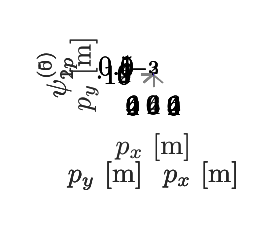
\begin{tikzpicture}

\begin{axis}[%
width=0.34\figurewidth,
height=0.7\figureheight,
at={(0\figurewidth,2\figureheight)},
scale only axis,
xmin=0,
xmax=6,
tick align=outside,
xlabel style={font=\color{white!15!black}},
xlabel={$p_x$~[m]},
ymin=0,
ymax=6,
ylabel style={font=\color{white!15!black}},
ylabel={$p_y$~[m]},
zmin=0,
zmax=0.001,
zlabel style={font=\color{white!15!black}},
zlabel={$\psi_{1\bm p}^{\text{(0)}}$},
view={-45}{25},
axis background/.style={fill=white},
axis x line*=bottom,
axis y line*=left,
axis z line*=left,
xmajorgrids,
ymajorgrids,
zmajorgrids
]

\addplot3[%
surf,
shader=interp, colormap={mymap}{[1pt] rgb(0pt)=(0.2422,0.1504,0.6603); rgb(1pt)=(0.25039,0.164995,0.707614); rgb(2pt)=(0.257771,0.181781,0.751138); rgb(3pt)=(0.264729,0.197757,0.795214); rgb(4pt)=(0.270648,0.214676,0.836371); rgb(5pt)=(0.275114,0.234238,0.870986); rgb(6pt)=(0.2783,0.255871,0.899071); rgb(7pt)=(0.280333,0.278233,0.9221); rgb(8pt)=(0.281338,0.300595,0.941376); rgb(9pt)=(0.281014,0.322757,0.957886); rgb(10pt)=(0.279467,0.344671,0.971676); rgb(11pt)=(0.275971,0.366681,0.982905); rgb(12pt)=(0.269914,0.3892,0.9906); rgb(13pt)=(0.260243,0.412329,0.995157); rgb(14pt)=(0.244033,0.435833,0.998833); rgb(15pt)=(0.220643,0.460257,0.997286); rgb(16pt)=(0.196333,0.484719,0.989152); rgb(17pt)=(0.183405,0.507371,0.979795); rgb(18pt)=(0.178643,0.528857,0.968157); rgb(19pt)=(0.176438,0.549905,0.952019); rgb(20pt)=(0.168743,0.570262,0.935871); rgb(21pt)=(0.154,0.5902,0.9218); rgb(22pt)=(0.146029,0.609119,0.907857); rgb(23pt)=(0.138024,0.627629,0.89729); rgb(24pt)=(0.124814,0.645929,0.888343); rgb(25pt)=(0.111252,0.6635,0.876314); rgb(26pt)=(0.0952095,0.679829,0.859781); rgb(27pt)=(0.0688714,0.694771,0.839357); rgb(28pt)=(0.0296667,0.708167,0.816333); rgb(29pt)=(0.00357143,0.720267,0.7917); rgb(30pt)=(0.00665714,0.731214,0.766014); rgb(31pt)=(0.0433286,0.741095,0.73941); rgb(32pt)=(0.0963952,0.75,0.712038); rgb(33pt)=(0.140771,0.7584,0.684157); rgb(34pt)=(0.1717,0.766962,0.655443); rgb(35pt)=(0.193767,0.775767,0.6251); rgb(36pt)=(0.216086,0.7843,0.5923); rgb(37pt)=(0.246957,0.791795,0.556743); rgb(38pt)=(0.290614,0.79729,0.518829); rgb(39pt)=(0.340643,0.8008,0.478857); rgb(40pt)=(0.3909,0.802871,0.435448); rgb(41pt)=(0.445629,0.802419,0.390919); rgb(42pt)=(0.5044,0.7993,0.348); rgb(43pt)=(0.561562,0.794233,0.304481); rgb(44pt)=(0.617395,0.787619,0.261238); rgb(45pt)=(0.671986,0.779271,0.2227); rgb(46pt)=(0.7242,0.769843,0.191029); rgb(47pt)=(0.773833,0.759805,0.16461); rgb(48pt)=(0.820314,0.749814,0.153529); rgb(49pt)=(0.863433,0.7406,0.159633); rgb(50pt)=(0.903543,0.733029,0.177414); rgb(51pt)=(0.939257,0.728786,0.209957); rgb(52pt)=(0.972757,0.729771,0.239443); rgb(53pt)=(0.995648,0.743371,0.237148); rgb(54pt)=(0.996986,0.765857,0.219943); rgb(55pt)=(0.995205,0.789252,0.202762); rgb(56pt)=(0.9892,0.813567,0.188533); rgb(57pt)=(0.978629,0.838629,0.176557); rgb(58pt)=(0.967648,0.8639,0.16429); rgb(59pt)=(0.96101,0.889019,0.153676); rgb(60pt)=(0.959671,0.913457,0.142257); rgb(61pt)=(0.962795,0.937338,0.12651); rgb(62pt)=(0.969114,0.960629,0.106362); rgb(63pt)=(0.9769,0.9839,0.0805)}, mesh/rows=61]
table[row sep=crcr, point meta=\thisrow{c}] {%
%
x	y	z	c\\
0	0	0.000546448087431694	0.000546448087431694\\
0	0.1	0.000546448087431694	0.000546448087431694\\
0	0.2	0.000546448087431694	0.000546448087431694\\
0	0.3	0.000546448087431694	0.000546448087431694\\
0	0.4	0.000546448087431694	0.000546448087431694\\
0	0.5	0.000546448087431694	0.000546448087431694\\
0	0.6	0.000546448087431694	0.000546448087431694\\
0	0.7	0.000546448087431694	0.000546448087431694\\
0	0.8	0.000546448087431694	0.000546448087431694\\
0	0.9	0.000546448087431694	0.000546448087431694\\
0	1	0.000546448087431694	0.000546448087431694\\
0	1.1	0.000546448087431694	0.000546448087431694\\
0	1.2	0.000546448087431694	0.000546448087431694\\
0	1.3	0.000546448087431694	0.000546448087431694\\
0	1.4	0.000546448087431694	0.000546448087431694\\
0	1.5	0.000546448087431694	0.000546448087431694\\
0	1.6	0.000546448087431694	0.000546448087431694\\
0	1.7	0.000546448087431694	0.000546448087431694\\
0	1.8	0.000546448087431694	0.000546448087431694\\
0	1.9	0.000546448087431694	0.000546448087431694\\
0	2	0.000546448087431694	0.000546448087431694\\
0	2.1	0.000546448087431694	0.000546448087431694\\
0	2.2	0.000546448087431694	0.000546448087431694\\
0	2.3	0.000546448087431694	0.000546448087431694\\
0	2.4	0.000546448087431694	0.000546448087431694\\
0	2.5	0.000546448087431694	0.000546448087431694\\
0	2.6	0.000546448087431694	0.000546448087431694\\
0	2.7	0.000546448087431694	0.000546448087431694\\
0	2.8	0.000546448087431694	0.000546448087431694\\
0	2.9	0.000546448087431694	0.000546448087431694\\
0	3	0.000546448087431694	0.000546448087431694\\
0	3.1	0.000546448087431694	0.000546448087431694\\
0	3.2	0.000546448087431694	0.000546448087431694\\
0	3.3	0.000546448087431694	0.000546448087431694\\
0	3.4	0.000546448087431694	0.000546448087431694\\
0	3.5	0.000546448087431694	0.000546448087431694\\
0	3.6	0.000546448087431694	0.000546448087431694\\
0	3.7	0.000546448087431694	0.000546448087431694\\
0	3.8	0.000546448087431694	0.000546448087431694\\
0	3.9	0.000546448087431694	0.000546448087431694\\
0	4	0.000546448087431694	0.000546448087431694\\
0	4.1	0.000546448087431694	0.000546448087431694\\
0	4.2	0.000546448087431694	0.000546448087431694\\
0	4.3	0.000546448087431694	0.000546448087431694\\
0	4.4	0.000546448087431694	0.000546448087431694\\
0	4.5	0.000546448087431694	0.000546448087431694\\
0	4.6	0.000546448087431694	0.000546448087431694\\
0	4.7	0.000546448087431694	0.000546448087431694\\
0	4.8	0.000546448087431694	0.000546448087431694\\
0	4.9	0.000546448087431694	0.000546448087431694\\
0	5	0.000546448087431694	0.000546448087431694\\
0	5.1	0.000546448087431694	0.000546448087431694\\
0	5.2	0.000546448087431694	0.000546448087431694\\
0	5.3	0.000546448087431694	0.000546448087431694\\
0	5.4	0.000546448087431694	0.000546448087431694\\
0	5.5	0.000546448087431694	0.000546448087431694\\
0	5.6	0.000546448087431694	0.000546448087431694\\
0	5.7	0.000546448087431694	0.000546448087431694\\
0	5.8	0.000546448087431694	0.000546448087431694\\
0	5.9	0.000546448087431694	0.000546448087431694\\
0	6	0.000546448087431694	0.000546448087431694\\
0.1	0	0.000546448087431694	0.000546448087431694\\
0.1	0.1	0.000546448087431694	0.000546448087431694\\
0.1	0.2	0.000546448087431694	0.000546448087431694\\
0.1	0.3	0.000546448087431694	0.000546448087431694\\
0.1	0.4	0.000546448087431694	0.000546448087431694\\
0.1	0.5	0.000546448087431694	0.000546448087431694\\
0.1	0.6	0.000546448087431694	0.000546448087431694\\
0.1	0.7	0.000546448087431694	0.000546448087431694\\
0.1	0.8	0.000546448087431694	0.000546448087431694\\
0.1	0.9	0.000546448087431694	0.000546448087431694\\
0.1	1	0.000546448087431694	0.000546448087431694\\
0.1	1.1	0.000546448087431694	0.000546448087431694\\
0.1	1.2	0.000546448087431694	0.000546448087431694\\
0.1	1.3	0.000546448087431694	0.000546448087431694\\
0.1	1.4	0.000546448087431694	0.000546448087431694\\
0.1	1.5	0.000546448087431694	0.000546448087431694\\
0.1	1.6	0.000546448087431694	0.000546448087431694\\
0.1	1.7	0.000546448087431694	0.000546448087431694\\
0.1	1.8	0.000546448087431694	0.000546448087431694\\
0.1	1.9	0.000546448087431694	0.000546448087431694\\
0.1	2	0.000546448087431694	0.000546448087431694\\
0.1	2.1	0.000546448087431694	0.000546448087431694\\
0.1	2.2	0.000546448087431694	0.000546448087431694\\
0.1	2.3	0.000546448087431694	0.000546448087431694\\
0.1	2.4	0.000546448087431694	0.000546448087431694\\
0.1	2.5	0.000546448087431694	0.000546448087431694\\
0.1	2.6	0.000546448087431694	0.000546448087431694\\
0.1	2.7	0.000546448087431694	0.000546448087431694\\
0.1	2.8	0.000546448087431694	0.000546448087431694\\
0.1	2.9	0.000546448087431694	0.000546448087431694\\
0.1	3	0.000546448087431694	0.000546448087431694\\
0.1	3.1	0.000546448087431694	0.000546448087431694\\
0.1	3.2	0.000546448087431694	0.000546448087431694\\
0.1	3.3	0.000546448087431694	0.000546448087431694\\
0.1	3.4	0.000546448087431694	0.000546448087431694\\
0.1	3.5	0.000546448087431694	0.000546448087431694\\
0.1	3.6	0.000546448087431694	0.000546448087431694\\
0.1	3.7	0.000546448087431694	0.000546448087431694\\
0.1	3.8	0.000546448087431694	0.000546448087431694\\
0.1	3.9	0.000546448087431694	0.000546448087431694\\
0.1	4	0.000546448087431694	0.000546448087431694\\
0.1	4.1	0.000546448087431694	0.000546448087431694\\
0.1	4.2	0.000546448087431694	0.000546448087431694\\
0.1	4.3	0.000546448087431694	0.000546448087431694\\
0.1	4.4	0.000546448087431694	0.000546448087431694\\
0.1	4.5	0.000546448087431694	0.000546448087431694\\
0.1	4.6	0.000546448087431694	0.000546448087431694\\
0.1	4.7	0.000546448087431694	0.000546448087431694\\
0.1	4.8	0.000546448087431694	0.000546448087431694\\
0.1	4.9	0.000546448087431694	0.000546448087431694\\
0.1	5	0.000546448087431694	0.000546448087431694\\
0.1	5.1	0.000546448087431694	0.000546448087431694\\
0.1	5.2	0.000546448087431694	0.000546448087431694\\
0.1	5.3	0.000546448087431694	0.000546448087431694\\
0.1	5.4	0.000546448087431694	0.000546448087431694\\
0.1	5.5	0.000546448087431694	0.000546448087431694\\
0.1	5.6	0.000546448087431694	0.000546448087431694\\
0.1	5.7	0.000546448087431694	0.000546448087431694\\
0.1	5.8	0.000546448087431694	0.000546448087431694\\
0.1	5.9	0.000546448087431694	0.000546448087431694\\
0.1	6	0.000546448087431694	0.000546448087431694\\
0.2	0	0.000546448087431694	0.000546448087431694\\
0.2	0.1	0.000546448087431694	0.000546448087431694\\
0.2	0.2	0.000546448087431694	0.000546448087431694\\
0.2	0.3	0.000546448087431694	0.000546448087431694\\
0.2	0.4	0.000546448087431694	0.000546448087431694\\
0.2	0.5	0.000546448087431694	0.000546448087431694\\
0.2	0.6	0.000546448087431694	0.000546448087431694\\
0.2	0.7	0.000546448087431694	0.000546448087431694\\
0.2	0.8	0.000546448087431694	0.000546448087431694\\
0.2	0.9	0.000546448087431694	0.000546448087431694\\
0.2	1	0.000546448087431694	0.000546448087431694\\
0.2	1.1	0.000546448087431694	0.000546448087431694\\
0.2	1.2	0.000546448087431694	0.000546448087431694\\
0.2	1.3	0.000546448087431694	0.000546448087431694\\
0.2	1.4	0.000546448087431694	0.000546448087431694\\
0.2	1.5	0.000546448087431694	0.000546448087431694\\
0.2	1.6	0.000546448087431694	0.000546448087431694\\
0.2	1.7	0.000546448087431694	0.000546448087431694\\
0.2	1.8	0.000546448087431694	0.000546448087431694\\
0.2	1.9	0.000546448087431694	0.000546448087431694\\
0.2	2	0.000546448087431694	0.000546448087431694\\
0.2	2.1	0.000546448087431694	0.000546448087431694\\
0.2	2.2	0.000546448087431694	0.000546448087431694\\
0.2	2.3	0.000546448087431694	0.000546448087431694\\
0.2	2.4	0.000546448087431694	0.000546448087431694\\
0.2	2.5	0.000546448087431694	0.000546448087431694\\
0.2	2.6	0.000546448087431694	0.000546448087431694\\
0.2	2.7	0.000546448087431694	0.000546448087431694\\
0.2	2.8	0.000546448087431694	0.000546448087431694\\
0.2	2.9	0.000546448087431694	0.000546448087431694\\
0.2	3	0.000546448087431694	0.000546448087431694\\
0.2	3.1	0.000546448087431694	0.000546448087431694\\
0.2	3.2	0.000546448087431694	0.000546448087431694\\
0.2	3.3	0.000546448087431694	0.000546448087431694\\
0.2	3.4	0.000546448087431694	0.000546448087431694\\
0.2	3.5	0.000546448087431694	0.000546448087431694\\
0.2	3.6	0.000546448087431694	0.000546448087431694\\
0.2	3.7	0.000546448087431694	0.000546448087431694\\
0.2	3.8	0.000546448087431694	0.000546448087431694\\
0.2	3.9	0.000546448087431694	0.000546448087431694\\
0.2	4	0.000546448087431694	0.000546448087431694\\
0.2	4.1	0.000546448087431694	0.000546448087431694\\
0.2	4.2	0.000546448087431694	0.000546448087431694\\
0.2	4.3	0.000546448087431694	0.000546448087431694\\
0.2	4.4	0.000546448087431694	0.000546448087431694\\
0.2	4.5	0.000546448087431694	0.000546448087431694\\
0.2	4.6	0.000546448087431694	0.000546448087431694\\
0.2	4.7	0.000546448087431694	0.000546448087431694\\
0.2	4.8	0.000546448087431694	0.000546448087431694\\
0.2	4.9	0.000546448087431694	0.000546448087431694\\
0.2	5	0.000546448087431694	0.000546448087431694\\
0.2	5.1	0.000546448087431694	0.000546448087431694\\
0.2	5.2	0.000546448087431694	0.000546448087431694\\
0.2	5.3	0.000546448087431694	0.000546448087431694\\
0.2	5.4	0.000546448087431694	0.000546448087431694\\
0.2	5.5	0.000546448087431694	0.000546448087431694\\
0.2	5.6	0.000546448087431694	0.000546448087431694\\
0.2	5.7	0.000546448087431694	0.000546448087431694\\
0.2	5.8	0.000546448087431694	0.000546448087431694\\
0.2	5.9	0.000546448087431694	0.000546448087431694\\
0.2	6	0.000546448087431694	0.000546448087431694\\
0.3	0	0.000546448087431694	0.000546448087431694\\
0.3	0.1	0.000546448087431694	0.000546448087431694\\
0.3	0.2	0.000546448087431694	0.000546448087431694\\
0.3	0.3	0.000546448087431694	0.000546448087431694\\
0.3	0.4	0.000546448087431694	0.000546448087431694\\
0.3	0.5	0.000546448087431694	0.000546448087431694\\
0.3	0.6	0.000546448087431694	0.000546448087431694\\
0.3	0.7	0.000546448087431694	0.000546448087431694\\
0.3	0.8	0.000546448087431694	0.000546448087431694\\
0.3	0.9	0.000546448087431694	0.000546448087431694\\
0.3	1	0.000546448087431694	0.000546448087431694\\
0.3	1.1	0.000546448087431694	0.000546448087431694\\
0.3	1.2	0.000546448087431694	0.000546448087431694\\
0.3	1.3	0.000546448087431694	0.000546448087431694\\
0.3	1.4	0.000546448087431694	0.000546448087431694\\
0.3	1.5	0.000546448087431694	0.000546448087431694\\
0.3	1.6	0.000546448087431694	0.000546448087431694\\
0.3	1.7	0.000546448087431694	0.000546448087431694\\
0.3	1.8	0.000546448087431694	0.000546448087431694\\
0.3	1.9	0.000546448087431694	0.000546448087431694\\
0.3	2	0.000546448087431694	0.000546448087431694\\
0.3	2.1	0.000546448087431694	0.000546448087431694\\
0.3	2.2	0.000546448087431694	0.000546448087431694\\
0.3	2.3	0.000546448087431694	0.000546448087431694\\
0.3	2.4	0.000546448087431694	0.000546448087431694\\
0.3	2.5	0.000546448087431694	0.000546448087431694\\
0.3	2.6	0.000546448087431694	0.000546448087431694\\
0.3	2.7	0.000546448087431694	0.000546448087431694\\
0.3	2.8	0.000546448087431694	0.000546448087431694\\
0.3	2.9	0.000546448087431694	0.000546448087431694\\
0.3	3	0.000546448087431694	0.000546448087431694\\
0.3	3.1	0.000546448087431694	0.000546448087431694\\
0.3	3.2	0.000546448087431694	0.000546448087431694\\
0.3	3.3	0.000546448087431694	0.000546448087431694\\
0.3	3.4	0.000546448087431694	0.000546448087431694\\
0.3	3.5	0.000546448087431694	0.000546448087431694\\
0.3	3.6	0.000546448087431694	0.000546448087431694\\
0.3	3.7	0.000546448087431694	0.000546448087431694\\
0.3	3.8	0.000546448087431694	0.000546448087431694\\
0.3	3.9	0.000546448087431694	0.000546448087431694\\
0.3	4	0.000546448087431694	0.000546448087431694\\
0.3	4.1	0.000546448087431694	0.000546448087431694\\
0.3	4.2	0.000546448087431694	0.000546448087431694\\
0.3	4.3	0.000546448087431694	0.000546448087431694\\
0.3	4.4	0.000546448087431694	0.000546448087431694\\
0.3	4.5	0.000546448087431694	0.000546448087431694\\
0.3	4.6	0.000546448087431694	0.000546448087431694\\
0.3	4.7	0.000546448087431694	0.000546448087431694\\
0.3	4.8	0.000546448087431694	0.000546448087431694\\
0.3	4.9	0.000546448087431694	0.000546448087431694\\
0.3	5	0.000546448087431694	0.000546448087431694\\
0.3	5.1	0.000546448087431694	0.000546448087431694\\
0.3	5.2	0.000546448087431694	0.000546448087431694\\
0.3	5.3	0.000546448087431694	0.000546448087431694\\
0.3	5.4	0.000546448087431694	0.000546448087431694\\
0.3	5.5	0.000546448087431694	0.000546448087431694\\
0.3	5.6	0.000546448087431694	0.000546448087431694\\
0.3	5.7	0.000546448087431694	0.000546448087431694\\
0.3	5.8	0.000546448087431694	0.000546448087431694\\
0.3	5.9	0.000546448087431694	0.000546448087431694\\
0.3	6	0.000546448087431694	0.000546448087431694\\
0.4	0	0.000546448087431694	0.000546448087431694\\
0.4	0.1	0.000546448087431694	0.000546448087431694\\
0.4	0.2	0.000546448087431694	0.000546448087431694\\
0.4	0.3	0.000546448087431694	0.000546448087431694\\
0.4	0.4	0.000546448087431694	0.000546448087431694\\
0.4	0.5	0.000546448087431694	0.000546448087431694\\
0.4	0.6	0.000546448087431694	0.000546448087431694\\
0.4	0.7	0.000546448087431694	0.000546448087431694\\
0.4	0.8	0.000546448087431694	0.000546448087431694\\
0.4	0.9	0.000546448087431694	0.000546448087431694\\
0.4	1	0.000546448087431694	0.000546448087431694\\
0.4	1.1	0.000546448087431694	0.000546448087431694\\
0.4	1.2	0.000546448087431694	0.000546448087431694\\
0.4	1.3	0.000546448087431694	0.000546448087431694\\
0.4	1.4	0.000546448087431694	0.000546448087431694\\
0.4	1.5	0.000546448087431694	0.000546448087431694\\
0.4	1.6	0.000546448087431694	0.000546448087431694\\
0.4	1.7	0.000546448087431694	0.000546448087431694\\
0.4	1.8	0.000546448087431694	0.000546448087431694\\
0.4	1.9	0.000546448087431694	0.000546448087431694\\
0.4	2	0.000546448087431694	0.000546448087431694\\
0.4	2.1	0.000546448087431694	0.000546448087431694\\
0.4	2.2	0.000546448087431694	0.000546448087431694\\
0.4	2.3	0.000546448087431694	0.000546448087431694\\
0.4	2.4	0.000546448087431694	0.000546448087431694\\
0.4	2.5	0.000546448087431694	0.000546448087431694\\
0.4	2.6	0.000546448087431694	0.000546448087431694\\
0.4	2.7	0.000546448087431694	0.000546448087431694\\
0.4	2.8	0.000546448087431694	0.000546448087431694\\
0.4	2.9	0.000546448087431694	0.000546448087431694\\
0.4	3	0.000546448087431694	0.000546448087431694\\
0.4	3.1	0.000546448087431694	0.000546448087431694\\
0.4	3.2	0.000546448087431694	0.000546448087431694\\
0.4	3.3	0.000546448087431694	0.000546448087431694\\
0.4	3.4	0.000546448087431694	0.000546448087431694\\
0.4	3.5	0.000546448087431694	0.000546448087431694\\
0.4	3.6	0.000546448087431694	0.000546448087431694\\
0.4	3.7	0.000546448087431694	0.000546448087431694\\
0.4	3.8	0.000546448087431694	0.000546448087431694\\
0.4	3.9	0.000546448087431694	0.000546448087431694\\
0.4	4	0.000546448087431694	0.000546448087431694\\
0.4	4.1	0.000546448087431694	0.000546448087431694\\
0.4	4.2	0.000546448087431694	0.000546448087431694\\
0.4	4.3	0.000546448087431694	0.000546448087431694\\
0.4	4.4	0.000546448087431694	0.000546448087431694\\
0.4	4.5	0.000546448087431694	0.000546448087431694\\
0.4	4.6	0.000546448087431694	0.000546448087431694\\
0.4	4.7	0.000546448087431694	0.000546448087431694\\
0.4	4.8	0.000546448087431694	0.000546448087431694\\
0.4	4.9	0.000546448087431694	0.000546448087431694\\
0.4	5	0.000546448087431694	0.000546448087431694\\
0.4	5.1	0.000546448087431694	0.000546448087431694\\
0.4	5.2	0.000546448087431694	0.000546448087431694\\
0.4	5.3	0.000546448087431694	0.000546448087431694\\
0.4	5.4	0.000546448087431694	0.000546448087431694\\
0.4	5.5	0.000546448087431694	0.000546448087431694\\
0.4	5.6	0.000546448087431694	0.000546448087431694\\
0.4	5.7	0.000546448087431694	0.000546448087431694\\
0.4	5.8	0.000546448087431694	0.000546448087431694\\
0.4	5.9	0.000546448087431694	0.000546448087431694\\
0.4	6	0.000546448087431694	0.000546448087431694\\
0.5	0	0.000546448087431694	0.000546448087431694\\
0.5	0.1	0.000546448087431694	0.000546448087431694\\
0.5	0.2	0.000546448087431694	0.000546448087431694\\
0.5	0.3	0.000546448087431694	0.000546448087431694\\
0.5	0.4	0.000546448087431694	0.000546448087431694\\
0.5	0.5	0.000546448087431694	0.000546448087431694\\
0.5	0.6	0.000546448087431694	0.000546448087431694\\
0.5	0.7	0.000546448087431694	0.000546448087431694\\
0.5	0.8	0.000546448087431694	0.000546448087431694\\
0.5	0.9	0.000546448087431694	0.000546448087431694\\
0.5	1	0.000546448087431694	0.000546448087431694\\
0.5	1.1	0.000546448087431694	0.000546448087431694\\
0.5	1.2	0.000546448087431694	0.000546448087431694\\
0.5	1.3	0.000546448087431694	0.000546448087431694\\
0.5	1.4	0.000546448087431694	0.000546448087431694\\
0.5	1.5	0.000546448087431694	0.000546448087431694\\
0.5	1.6	0.000546448087431694	0.000546448087431694\\
0.5	1.7	0.000546448087431694	0.000546448087431694\\
0.5	1.8	0.000546448087431694	0.000546448087431694\\
0.5	1.9	0.000546448087431694	0.000546448087431694\\
0.5	2	0.000546448087431694	0.000546448087431694\\
0.5	2.1	0.000546448087431694	0.000546448087431694\\
0.5	2.2	0.000546448087431694	0.000546448087431694\\
0.5	2.3	0.000546448087431694	0.000546448087431694\\
0.5	2.4	0.000546448087431694	0.000546448087431694\\
0.5	2.5	0.000546448087431694	0.000546448087431694\\
0.5	2.6	0.000546448087431694	0.000546448087431694\\
0.5	2.7	0.000546448087431694	0.000546448087431694\\
0.5	2.8	0.000546448087431694	0.000546448087431694\\
0.5	2.9	0.000546448087431694	0.000546448087431694\\
0.5	3	0.000546448087431694	0.000546448087431694\\
0.5	3.1	0.000546448087431694	0.000546448087431694\\
0.5	3.2	0.000546448087431694	0.000546448087431694\\
0.5	3.3	0.000546448087431694	0.000546448087431694\\
0.5	3.4	0.000546448087431694	0.000546448087431694\\
0.5	3.5	0.000546448087431694	0.000546448087431694\\
0.5	3.6	0.000546448087431694	0.000546448087431694\\
0.5	3.7	0.000546448087431694	0.000546448087431694\\
0.5	3.8	0.000546448087431694	0.000546448087431694\\
0.5	3.9	0.000546448087431694	0.000546448087431694\\
0.5	4	0.000546448087431694	0.000546448087431694\\
0.5	4.1	0.000546448087431694	0.000546448087431694\\
0.5	4.2	0.000546448087431694	0.000546448087431694\\
0.5	4.3	0.000546448087431694	0.000546448087431694\\
0.5	4.4	0.000546448087431694	0.000546448087431694\\
0.5	4.5	0.000546448087431694	0.000546448087431694\\
0.5	4.6	0.000546448087431694	0.000546448087431694\\
0.5	4.7	0.000546448087431694	0.000546448087431694\\
0.5	4.8	0.000546448087431694	0.000546448087431694\\
0.5	4.9	0.000546448087431694	0.000546448087431694\\
0.5	5	0.000546448087431694	0.000546448087431694\\
0.5	5.1	0.000546448087431694	0.000546448087431694\\
0.5	5.2	0.000546448087431694	0.000546448087431694\\
0.5	5.3	0.000546448087431694	0.000546448087431694\\
0.5	5.4	0.000546448087431694	0.000546448087431694\\
0.5	5.5	0.000546448087431694	0.000546448087431694\\
0.5	5.6	0.000546448087431694	0.000546448087431694\\
0.5	5.7	0.000546448087431694	0.000546448087431694\\
0.5	5.8	0.000546448087431694	0.000546448087431694\\
0.5	5.9	0.000546448087431694	0.000546448087431694\\
0.5	6	0.000546448087431694	0.000546448087431694\\
0.6	0	0.000546448087431694	0.000546448087431694\\
0.6	0.1	0.000546448087431694	0.000546448087431694\\
0.6	0.2	0.000546448087431694	0.000546448087431694\\
0.6	0.3	0.000546448087431694	0.000546448087431694\\
0.6	0.4	0.000546448087431694	0.000546448087431694\\
0.6	0.5	0.000546448087431694	0.000546448087431694\\
0.6	0.6	0.000546448087431694	0.000546448087431694\\
0.6	0.7	0.000546448087431694	0.000546448087431694\\
0.6	0.8	0.000546448087431694	0.000546448087431694\\
0.6	0.9	0.000546448087431694	0.000546448087431694\\
0.6	1	0.000546448087431694	0.000546448087431694\\
0.6	1.1	0.000546448087431694	0.000546448087431694\\
0.6	1.2	0.000546448087431694	0.000546448087431694\\
0.6	1.3	0.000546448087431694	0.000546448087431694\\
0.6	1.4	0.000546448087431694	0.000546448087431694\\
0.6	1.5	0.000546448087431694	0.000546448087431694\\
0.6	1.6	0.000546448087431694	0.000546448087431694\\
0.6	1.7	0.000546448087431694	0.000546448087431694\\
0.6	1.8	0.000546448087431694	0.000546448087431694\\
0.6	1.9	0.000546448087431694	0.000546448087431694\\
0.6	2	0.000546448087431694	0.000546448087431694\\
0.6	2.1	0.000546448087431694	0.000546448087431694\\
0.6	2.2	0.000546448087431694	0.000546448087431694\\
0.6	2.3	0.000546448087431694	0.000546448087431694\\
0.6	2.4	0.000546448087431694	0.000546448087431694\\
0.6	2.5	0.000546448087431694	0.000546448087431694\\
0.6	2.6	0.000546448087431694	0.000546448087431694\\
0.6	2.7	0.000546448087431694	0.000546448087431694\\
0.6	2.8	0.000546448087431694	0.000546448087431694\\
0.6	2.9	0.000546448087431694	0.000546448087431694\\
0.6	3	0.000546448087431694	0.000546448087431694\\
0.6	3.1	0.000546448087431694	0.000546448087431694\\
0.6	3.2	0.000546448087431694	0.000546448087431694\\
0.6	3.3	0.000546448087431694	0.000546448087431694\\
0.6	3.4	0.000546448087431694	0.000546448087431694\\
0.6	3.5	0.000546448087431694	0.000546448087431694\\
0.6	3.6	0.000546448087431694	0.000546448087431694\\
0.6	3.7	0.000546448087431694	0.000546448087431694\\
0.6	3.8	0.000546448087431694	0.000546448087431694\\
0.6	3.9	0.000546448087431694	0.000546448087431694\\
0.6	4	0.000546448087431694	0.000546448087431694\\
0.6	4.1	0.000546448087431694	0.000546448087431694\\
0.6	4.2	0.000546448087431694	0.000546448087431694\\
0.6	4.3	0.000546448087431694	0.000546448087431694\\
0.6	4.4	0.000546448087431694	0.000546448087431694\\
0.6	4.5	0.000546448087431694	0.000546448087431694\\
0.6	4.6	0.000546448087431694	0.000546448087431694\\
0.6	4.7	0.000546448087431694	0.000546448087431694\\
0.6	4.8	0.000546448087431694	0.000546448087431694\\
0.6	4.9	0.000546448087431694	0.000546448087431694\\
0.6	5	0.000546448087431694	0.000546448087431694\\
0.6	5.1	0.000546448087431694	0.000546448087431694\\
0.6	5.2	0.000546448087431694	0.000546448087431694\\
0.6	5.3	0.000546448087431694	0.000546448087431694\\
0.6	5.4	0.000546448087431694	0.000546448087431694\\
0.6	5.5	0.000546448087431694	0.000546448087431694\\
0.6	5.6	0.000546448087431694	0.000546448087431694\\
0.6	5.7	0.000546448087431694	0.000546448087431694\\
0.6	5.8	0.000546448087431694	0.000546448087431694\\
0.6	5.9	0.000546448087431694	0.000546448087431694\\
0.6	6	0.000546448087431694	0.000546448087431694\\
0.7	0	0.000546448087431694	0.000546448087431694\\
0.7	0.1	0.000546448087431694	0.000546448087431694\\
0.7	0.2	0.000546448087431694	0.000546448087431694\\
0.7	0.3	0.000546448087431694	0.000546448087431694\\
0.7	0.4	0.000546448087431694	0.000546448087431694\\
0.7	0.5	0.000546448087431694	0.000546448087431694\\
0.7	0.6	0.000546448087431694	0.000546448087431694\\
0.7	0.7	0.000546448087431694	0.000546448087431694\\
0.7	0.8	0.000546448087431694	0.000546448087431694\\
0.7	0.9	0.000546448087431694	0.000546448087431694\\
0.7	1	0.000546448087431694	0.000546448087431694\\
0.7	1.1	0.000546448087431694	0.000546448087431694\\
0.7	1.2	0.000546448087431694	0.000546448087431694\\
0.7	1.3	0.000546448087431694	0.000546448087431694\\
0.7	1.4	0.000546448087431694	0.000546448087431694\\
0.7	1.5	0.000546448087431694	0.000546448087431694\\
0.7	1.6	0.000546448087431694	0.000546448087431694\\
0.7	1.7	0.000546448087431694	0.000546448087431694\\
0.7	1.8	0.000546448087431694	0.000546448087431694\\
0.7	1.9	0.000546448087431694	0.000546448087431694\\
0.7	2	0.000546448087431694	0.000546448087431694\\
0.7	2.1	0.000546448087431694	0.000546448087431694\\
0.7	2.2	0.000546448087431694	0.000546448087431694\\
0.7	2.3	0.000546448087431694	0.000546448087431694\\
0.7	2.4	0.000546448087431694	0.000546448087431694\\
0.7	2.5	0.000546448087431694	0.000546448087431694\\
0.7	2.6	0.000546448087431694	0.000546448087431694\\
0.7	2.7	0.000546448087431694	0.000546448087431694\\
0.7	2.8	0.000546448087431694	0.000546448087431694\\
0.7	2.9	0.000546448087431694	0.000546448087431694\\
0.7	3	0.000546448087431694	0.000546448087431694\\
0.7	3.1	0.000546448087431694	0.000546448087431694\\
0.7	3.2	0.000546448087431694	0.000546448087431694\\
0.7	3.3	0.000546448087431694	0.000546448087431694\\
0.7	3.4	0.000546448087431694	0.000546448087431694\\
0.7	3.5	0.000546448087431694	0.000546448087431694\\
0.7	3.6	0.000546448087431694	0.000546448087431694\\
0.7	3.7	0.000546448087431694	0.000546448087431694\\
0.7	3.8	0.000546448087431694	0.000546448087431694\\
0.7	3.9	0.000546448087431694	0.000546448087431694\\
0.7	4	0.000546448087431694	0.000546448087431694\\
0.7	4.1	0.000546448087431694	0.000546448087431694\\
0.7	4.2	0.000546448087431694	0.000546448087431694\\
0.7	4.3	0.000546448087431694	0.000546448087431694\\
0.7	4.4	0.000546448087431694	0.000546448087431694\\
0.7	4.5	0.000546448087431694	0.000546448087431694\\
0.7	4.6	0.000546448087431694	0.000546448087431694\\
0.7	4.7	0.000546448087431694	0.000546448087431694\\
0.7	4.8	0.000546448087431694	0.000546448087431694\\
0.7	4.9	0.000546448087431694	0.000546448087431694\\
0.7	5	0.000546448087431694	0.000546448087431694\\
0.7	5.1	0.000546448087431694	0.000546448087431694\\
0.7	5.2	0.000546448087431694	0.000546448087431694\\
0.7	5.3	0.000546448087431694	0.000546448087431694\\
0.7	5.4	0.000546448087431694	0.000546448087431694\\
0.7	5.5	0.000546448087431694	0.000546448087431694\\
0.7	5.6	0.000546448087431694	0.000546448087431694\\
0.7	5.7	0.000546448087431694	0.000546448087431694\\
0.7	5.8	0.000546448087431694	0.000546448087431694\\
0.7	5.9	0.000546448087431694	0.000546448087431694\\
0.7	6	0.000546448087431694	0.000546448087431694\\
0.8	0	0.000546448087431694	0.000546448087431694\\
0.8	0.1	0.000546448087431694	0.000546448087431694\\
0.8	0.2	0.000546448087431694	0.000546448087431694\\
0.8	0.3	0.000546448087431694	0.000546448087431694\\
0.8	0.4	0.000546448087431694	0.000546448087431694\\
0.8	0.5	0.000546448087431694	0.000546448087431694\\
0.8	0.6	0.000546448087431694	0.000546448087431694\\
0.8	0.7	0.000546448087431694	0.000546448087431694\\
0.8	0.8	0.000546448087431694	0.000546448087431694\\
0.8	0.9	0.000546448087431694	0.000546448087431694\\
0.8	1	0.000546448087431694	0.000546448087431694\\
0.8	1.1	0.000546448087431694	0.000546448087431694\\
0.8	1.2	0.000546448087431694	0.000546448087431694\\
0.8	1.3	0.000546448087431694	0.000546448087431694\\
0.8	1.4	0.000546448087431694	0.000546448087431694\\
0.8	1.5	0.000546448087431694	0.000546448087431694\\
0.8	1.6	0.000546448087431694	0.000546448087431694\\
0.8	1.7	0.000546448087431694	0.000546448087431694\\
0.8	1.8	0.000546448087431694	0.000546448087431694\\
0.8	1.9	0.000546448087431694	0.000546448087431694\\
0.8	2	0.000546448087431694	0.000546448087431694\\
0.8	2.1	0.000546448087431694	0.000546448087431694\\
0.8	2.2	0.000546448087431694	0.000546448087431694\\
0.8	2.3	0.000546448087431694	0.000546448087431694\\
0.8	2.4	0.000546448087431694	0.000546448087431694\\
0.8	2.5	0.000546448087431694	0.000546448087431694\\
0.8	2.6	0.000546448087431694	0.000546448087431694\\
0.8	2.7	0.000546448087431694	0.000546448087431694\\
0.8	2.8	0.000546448087431694	0.000546448087431694\\
0.8	2.9	0.000546448087431694	0.000546448087431694\\
0.8	3	0.000546448087431694	0.000546448087431694\\
0.8	3.1	0.000546448087431694	0.000546448087431694\\
0.8	3.2	0.000546448087431694	0.000546448087431694\\
0.8	3.3	0.000546448087431694	0.000546448087431694\\
0.8	3.4	0.000546448087431694	0.000546448087431694\\
0.8	3.5	0.000546448087431694	0.000546448087431694\\
0.8	3.6	0.000546448087431694	0.000546448087431694\\
0.8	3.7	0.000546448087431694	0.000546448087431694\\
0.8	3.8	0.000546448087431694	0.000546448087431694\\
0.8	3.9	0.000546448087431694	0.000546448087431694\\
0.8	4	0.000546448087431694	0.000546448087431694\\
0.8	4.1	0.000546448087431694	0.000546448087431694\\
0.8	4.2	0.000546448087431694	0.000546448087431694\\
0.8	4.3	0.000546448087431694	0.000546448087431694\\
0.8	4.4	0.000546448087431694	0.000546448087431694\\
0.8	4.5	0.000546448087431694	0.000546448087431694\\
0.8	4.6	0.000546448087431694	0.000546448087431694\\
0.8	4.7	0.000546448087431694	0.000546448087431694\\
0.8	4.8	0.000546448087431694	0.000546448087431694\\
0.8	4.9	0.000546448087431694	0.000546448087431694\\
0.8	5	0.000546448087431694	0.000546448087431694\\
0.8	5.1	0.000546448087431694	0.000546448087431694\\
0.8	5.2	0.000546448087431694	0.000546448087431694\\
0.8	5.3	0.000546448087431694	0.000546448087431694\\
0.8	5.4	0.000546448087431694	0.000546448087431694\\
0.8	5.5	0.000546448087431694	0.000546448087431694\\
0.8	5.6	0.000546448087431694	0.000546448087431694\\
0.8	5.7	0.000546448087431694	0.000546448087431694\\
0.8	5.8	0.000546448087431694	0.000546448087431694\\
0.8	5.9	0.000546448087431694	0.000546448087431694\\
0.8	6	0.000546448087431694	0.000546448087431694\\
0.9	0	0.000546448087431694	0.000546448087431694\\
0.9	0.1	0.000546448087431694	0.000546448087431694\\
0.9	0.2	0.000546448087431694	0.000546448087431694\\
0.9	0.3	0.000546448087431694	0.000546448087431694\\
0.9	0.4	0.000546448087431694	0.000546448087431694\\
0.9	0.5	0.000546448087431694	0.000546448087431694\\
0.9	0.6	0.000546448087431694	0.000546448087431694\\
0.9	0.7	0.000546448087431694	0.000546448087431694\\
0.9	0.8	0.000546448087431694	0.000546448087431694\\
0.9	0.9	0.000546448087431694	0.000546448087431694\\
0.9	1	0.000546448087431694	0.000546448087431694\\
0.9	1.1	0.000546448087431694	0.000546448087431694\\
0.9	1.2	0.000546448087431694	0.000546448087431694\\
0.9	1.3	0.000546448087431694	0.000546448087431694\\
0.9	1.4	0.000546448087431694	0.000546448087431694\\
0.9	1.5	0.000546448087431694	0.000546448087431694\\
0.9	1.6	0.000546448087431694	0.000546448087431694\\
0.9	1.7	0.000546448087431694	0.000546448087431694\\
0.9	1.8	0.000546448087431694	0.000546448087431694\\
0.9	1.9	0.000546448087431694	0.000546448087431694\\
0.9	2	0.000546448087431694	0.000546448087431694\\
0.9	2.1	0.000546448087431694	0.000546448087431694\\
0.9	2.2	0.000546448087431694	0.000546448087431694\\
0.9	2.3	0.000546448087431694	0.000546448087431694\\
0.9	2.4	0.000546448087431694	0.000546448087431694\\
0.9	2.5	0.000546448087431694	0.000546448087431694\\
0.9	2.6	0.000546448087431694	0.000546448087431694\\
0.9	2.7	0.000546448087431694	0.000546448087431694\\
0.9	2.8	0.000546448087431694	0.000546448087431694\\
0.9	2.9	0.000546448087431694	0.000546448087431694\\
0.9	3	0.000546448087431694	0.000546448087431694\\
0.9	3.1	0.000546448087431694	0.000546448087431694\\
0.9	3.2	0.000546448087431694	0.000546448087431694\\
0.9	3.3	0.000546448087431694	0.000546448087431694\\
0.9	3.4	0.000546448087431694	0.000546448087431694\\
0.9	3.5	0.000546448087431694	0.000546448087431694\\
0.9	3.6	0.000546448087431694	0.000546448087431694\\
0.9	3.7	0.000546448087431694	0.000546448087431694\\
0.9	3.8	0.000546448087431694	0.000546448087431694\\
0.9	3.9	0.000546448087431694	0.000546448087431694\\
0.9	4	0.000546448087431694	0.000546448087431694\\
0.9	4.1	0.000546448087431694	0.000546448087431694\\
0.9	4.2	0.000546448087431694	0.000546448087431694\\
0.9	4.3	0.000546448087431694	0.000546448087431694\\
0.9	4.4	0.000546448087431694	0.000546448087431694\\
0.9	4.5	0.000546448087431694	0.000546448087431694\\
0.9	4.6	0.000546448087431694	0.000546448087431694\\
0.9	4.7	0.000546448087431694	0.000546448087431694\\
0.9	4.8	0.000546448087431694	0.000546448087431694\\
0.9	4.9	0.000546448087431694	0.000546448087431694\\
0.9	5	0.000546448087431694	0.000546448087431694\\
0.9	5.1	0.000546448087431694	0.000546448087431694\\
0.9	5.2	0.000546448087431694	0.000546448087431694\\
0.9	5.3	0.000546448087431694	0.000546448087431694\\
0.9	5.4	0.000546448087431694	0.000546448087431694\\
0.9	5.5	0.000546448087431694	0.000546448087431694\\
0.9	5.6	0.000546448087431694	0.000546448087431694\\
0.9	5.7	0.000546448087431694	0.000546448087431694\\
0.9	5.8	0.000546448087431694	0.000546448087431694\\
0.9	5.9	0.000546448087431694	0.000546448087431694\\
0.9	6	0.000546448087431694	0.000546448087431694\\
1	0	0.000546448087431694	0.000546448087431694\\
1	0.1	0.000546448087431694	0.000546448087431694\\
1	0.2	0.000546448087431694	0.000546448087431694\\
1	0.3	0.000546448087431694	0.000546448087431694\\
1	0.4	0.000546448087431694	0.000546448087431694\\
1	0.5	0.000546448087431694	0.000546448087431694\\
1	0.6	0.000546448087431694	0.000546448087431694\\
1	0.7	0.000546448087431694	0.000546448087431694\\
1	0.8	0.000546448087431694	0.000546448087431694\\
1	0.9	0.000546448087431694	0.000546448087431694\\
1	1	0.000546448087431694	0.000546448087431694\\
1	1.1	0.000546448087431694	0.000546448087431694\\
1	1.2	0.000546448087431694	0.000546448087431694\\
1	1.3	0.000546448087431694	0.000546448087431694\\
1	1.4	0.000546448087431694	0.000546448087431694\\
1	1.5	0.000546448087431694	0.000546448087431694\\
1	1.6	0.000546448087431694	0.000546448087431694\\
1	1.7	0.000546448087431694	0.000546448087431694\\
1	1.8	0.000546448087431694	0.000546448087431694\\
1	1.9	0.000546448087431694	0.000546448087431694\\
1	2	0.000546448087431694	0.000546448087431694\\
1	2.1	0.000546448087431694	0.000546448087431694\\
1	2.2	0.000546448087431694	0.000546448087431694\\
1	2.3	0.000546448087431694	0.000546448087431694\\
1	2.4	0.000546448087431694	0.000546448087431694\\
1	2.5	0.000546448087431694	0.000546448087431694\\
1	2.6	0.000546448087431694	0.000546448087431694\\
1	2.7	0.000546448087431694	0.000546448087431694\\
1	2.8	0.000546448087431694	0.000546448087431694\\
1	2.9	0.000546448087431694	0.000546448087431694\\
1	3	0.000546448087431694	0.000546448087431694\\
1	3.1	0.000546448087431694	0.000546448087431694\\
1	3.2	0.000546448087431694	0.000546448087431694\\
1	3.3	0.000546448087431694	0.000546448087431694\\
1	3.4	0.000546448087431694	0.000546448087431694\\
1	3.5	0.000546448087431694	0.000546448087431694\\
1	3.6	0.000546448087431694	0.000546448087431694\\
1	3.7	0.000546448087431694	0.000546448087431694\\
1	3.8	0.000546448087431694	0.000546448087431694\\
1	3.9	0.000546448087431694	0.000546448087431694\\
1	4	0.000546448087431694	0.000546448087431694\\
1	4.1	0.000546448087431694	0.000546448087431694\\
1	4.2	0.000546448087431694	0.000546448087431694\\
1	4.3	0.000546448087431694	0.000546448087431694\\
1	4.4	0.000546448087431694	0.000546448087431694\\
1	4.5	0.000546448087431694	0.000546448087431694\\
1	4.6	0.000546448087431694	0.000546448087431694\\
1	4.7	0.000546448087431694	0.000546448087431694\\
1	4.8	0.000546448087431694	0.000546448087431694\\
1	4.9	0.000546448087431694	0.000546448087431694\\
1	5	0.000546448087431694	0.000546448087431694\\
1	5.1	0.000546448087431694	0.000546448087431694\\
1	5.2	0.000546448087431694	0.000546448087431694\\
1	5.3	0.000546448087431694	0.000546448087431694\\
1	5.4	0.000546448087431694	0.000546448087431694\\
1	5.5	0.000546448087431694	0.000546448087431694\\
1	5.6	0.000546448087431694	0.000546448087431694\\
1	5.7	0.000546448087431694	0.000546448087431694\\
1	5.8	0.000546448087431694	0.000546448087431694\\
1	5.9	0.000546448087431694	0.000546448087431694\\
1	6	0.000546448087431694	0.000546448087431694\\
1.1	0	0.000546448087431694	0.000546448087431694\\
1.1	0.1	0.000546448087431694	0.000546448087431694\\
1.1	0.2	0.000546448087431694	0.000546448087431694\\
1.1	0.3	0.000546448087431694	0.000546448087431694\\
1.1	0.4	0.000546448087431694	0.000546448087431694\\
1.1	0.5	0.000546448087431694	0.000546448087431694\\
1.1	0.6	0.000546448087431694	0.000546448087431694\\
1.1	0.7	0.000546448087431694	0.000546448087431694\\
1.1	0.8	0.000546448087431694	0.000546448087431694\\
1.1	0.9	0.000546448087431694	0.000546448087431694\\
1.1	1	0.000546448087431694	0.000546448087431694\\
1.1	1.1	0.000546448087431694	0.000546448087431694\\
1.1	1.2	0.000546448087431694	0.000546448087431694\\
1.1	1.3	0.000546448087431694	0.000546448087431694\\
1.1	1.4	0.000546448087431694	0.000546448087431694\\
1.1	1.5	0.000546448087431694	0.000546448087431694\\
1.1	1.6	0.000546448087431694	0.000546448087431694\\
1.1	1.7	0.000546448087431694	0.000546448087431694\\
1.1	1.8	0.000546448087431694	0.000546448087431694\\
1.1	1.9	0.000546448087431694	0.000546448087431694\\
1.1	2	0.000546448087431694	0.000546448087431694\\
1.1	2.1	0.000546448087431694	0.000546448087431694\\
1.1	2.2	0.000546448087431694	0.000546448087431694\\
1.1	2.3	0.000546448087431694	0.000546448087431694\\
1.1	2.4	0.000546448087431694	0.000546448087431694\\
1.1	2.5	0.000546448087431694	0.000546448087431694\\
1.1	2.6	0.000546448087431694	0.000546448087431694\\
1.1	2.7	0.000546448087431694	0.000546448087431694\\
1.1	2.8	0.000546448087431694	0.000546448087431694\\
1.1	2.9	0.000546448087431694	0.000546448087431694\\
1.1	3	0.000546448087431694	0.000546448087431694\\
1.1	3.1	0.000546448087431694	0.000546448087431694\\
1.1	3.2	0.000546448087431694	0.000546448087431694\\
1.1	3.3	0.000546448087431694	0.000546448087431694\\
1.1	3.4	0.000546448087431694	0.000546448087431694\\
1.1	3.5	0.000546448087431694	0.000546448087431694\\
1.1	3.6	0.000546448087431694	0.000546448087431694\\
1.1	3.7	0.000546448087431694	0.000546448087431694\\
1.1	3.8	0.000546448087431694	0.000546448087431694\\
1.1	3.9	0.000546448087431694	0.000546448087431694\\
1.1	4	0.000546448087431694	0.000546448087431694\\
1.1	4.1	0.000546448087431694	0.000546448087431694\\
1.1	4.2	0.000546448087431694	0.000546448087431694\\
1.1	4.3	0.000546448087431694	0.000546448087431694\\
1.1	4.4	0.000546448087431694	0.000546448087431694\\
1.1	4.5	0.000546448087431694	0.000546448087431694\\
1.1	4.6	0.000546448087431694	0.000546448087431694\\
1.1	4.7	0.000546448087431694	0.000546448087431694\\
1.1	4.8	0.000546448087431694	0.000546448087431694\\
1.1	4.9	0.000546448087431694	0.000546448087431694\\
1.1	5	0.000546448087431694	0.000546448087431694\\
1.1	5.1	0.000546448087431694	0.000546448087431694\\
1.1	5.2	0.000546448087431694	0.000546448087431694\\
1.1	5.3	0.000546448087431694	0.000546448087431694\\
1.1	5.4	0.000546448087431694	0.000546448087431694\\
1.1	5.5	0.000546448087431694	0.000546448087431694\\
1.1	5.6	0.000546448087431694	0.000546448087431694\\
1.1	5.7	0.000546448087431694	0.000546448087431694\\
1.1	5.8	0.000546448087431694	0.000546448087431694\\
1.1	5.9	0.000546448087431694	0.000546448087431694\\
1.1	6	0.000546448087431694	0.000546448087431694\\
1.2	0	0.000546448087431694	0.000546448087431694\\
1.2	0.1	0.000546448087431694	0.000546448087431694\\
1.2	0.2	0.000546448087431694	0.000546448087431694\\
1.2	0.3	0.000546448087431694	0.000546448087431694\\
1.2	0.4	0.000546448087431694	0.000546448087431694\\
1.2	0.5	0.000546448087431694	0.000546448087431694\\
1.2	0.6	0.000546448087431694	0.000546448087431694\\
1.2	0.7	0.000546448087431694	0.000546448087431694\\
1.2	0.8	0.000546448087431694	0.000546448087431694\\
1.2	0.9	0.000546448087431694	0.000546448087431694\\
1.2	1	0.000546448087431694	0.000546448087431694\\
1.2	1.1	0.000546448087431694	0.000546448087431694\\
1.2	1.2	0.000546448087431694	0.000546448087431694\\
1.2	1.3	0.000546448087431694	0.000546448087431694\\
1.2	1.4	0.000546448087431694	0.000546448087431694\\
1.2	1.5	0.000546448087431694	0.000546448087431694\\
1.2	1.6	0.000546448087431694	0.000546448087431694\\
1.2	1.7	0.000546448087431694	0.000546448087431694\\
1.2	1.8	0.000546448087431694	0.000546448087431694\\
1.2	1.9	0.000546448087431694	0.000546448087431694\\
1.2	2	0.000546448087431694	0.000546448087431694\\
1.2	2.1	0.000546448087431694	0.000546448087431694\\
1.2	2.2	0.000546448087431694	0.000546448087431694\\
1.2	2.3	0.000546448087431694	0.000546448087431694\\
1.2	2.4	0.000546448087431694	0.000546448087431694\\
1.2	2.5	0.000546448087431694	0.000546448087431694\\
1.2	2.6	0.000546448087431694	0.000546448087431694\\
1.2	2.7	0.000546448087431694	0.000546448087431694\\
1.2	2.8	0.000546448087431694	0.000546448087431694\\
1.2	2.9	0.000546448087431694	0.000546448087431694\\
1.2	3	0.000546448087431694	0.000546448087431694\\
1.2	3.1	0.000546448087431694	0.000546448087431694\\
1.2	3.2	0.000546448087431694	0.000546448087431694\\
1.2	3.3	0.000546448087431694	0.000546448087431694\\
1.2	3.4	0.000546448087431694	0.000546448087431694\\
1.2	3.5	0.000546448087431694	0.000546448087431694\\
1.2	3.6	0.000546448087431694	0.000546448087431694\\
1.2	3.7	0.000546448087431694	0.000546448087431694\\
1.2	3.8	0.000546448087431694	0.000546448087431694\\
1.2	3.9	0.000546448087431694	0.000546448087431694\\
1.2	4	0.000546448087431694	0.000546448087431694\\
1.2	4.1	0.000546448087431694	0.000546448087431694\\
1.2	4.2	0.000546448087431694	0.000546448087431694\\
1.2	4.3	0.000546448087431694	0.000546448087431694\\
1.2	4.4	0.000546448087431694	0.000546448087431694\\
1.2	4.5	0.000546448087431694	0.000546448087431694\\
1.2	4.6	0.000546448087431694	0.000546448087431694\\
1.2	4.7	0.000546448087431694	0.000546448087431694\\
1.2	4.8	0.000546448087431694	0.000546448087431694\\
1.2	4.9	0.000546448087431694	0.000546448087431694\\
1.2	5	0.000546448087431694	0.000546448087431694\\
1.2	5.1	0.000546448087431694	0.000546448087431694\\
1.2	5.2	0.000546448087431694	0.000546448087431694\\
1.2	5.3	0.000546448087431694	0.000546448087431694\\
1.2	5.4	0.000546448087431694	0.000546448087431694\\
1.2	5.5	0.000546448087431694	0.000546448087431694\\
1.2	5.6	0.000546448087431694	0.000546448087431694\\
1.2	5.7	0.000546448087431694	0.000546448087431694\\
1.2	5.8	0.000546448087431694	0.000546448087431694\\
1.2	5.9	0.000546448087431694	0.000546448087431694\\
1.2	6	0.000546448087431694	0.000546448087431694\\
1.3	0	0.000546448087431694	0.000546448087431694\\
1.3	0.1	0.000546448087431694	0.000546448087431694\\
1.3	0.2	0.000546448087431694	0.000546448087431694\\
1.3	0.3	0.000546448087431694	0.000546448087431694\\
1.3	0.4	0.000546448087431694	0.000546448087431694\\
1.3	0.5	0.000546448087431694	0.000546448087431694\\
1.3	0.6	0.000546448087431694	0.000546448087431694\\
1.3	0.7	0.000546448087431694	0.000546448087431694\\
1.3	0.8	0.000546448087431694	0.000546448087431694\\
1.3	0.9	0.000546448087431694	0.000546448087431694\\
1.3	1	0.000546448087431694	0.000546448087431694\\
1.3	1.1	0.000546448087431694	0.000546448087431694\\
1.3	1.2	0.000546448087431694	0.000546448087431694\\
1.3	1.3	0.000546448087431694	0.000546448087431694\\
1.3	1.4	0.000546448087431694	0.000546448087431694\\
1.3	1.5	0.000546448087431694	0.000546448087431694\\
1.3	1.6	0.000546448087431694	0.000546448087431694\\
1.3	1.7	0.000546448087431694	0.000546448087431694\\
1.3	1.8	0.000546448087431694	0.000546448087431694\\
1.3	1.9	0.000546448087431694	0.000546448087431694\\
1.3	2	0.000546448087431694	0.000546448087431694\\
1.3	2.1	0.000546448087431694	0.000546448087431694\\
1.3	2.2	0.000546448087431694	0.000546448087431694\\
1.3	2.3	0.000546448087431694	0.000546448087431694\\
1.3	2.4	0.000546448087431694	0.000546448087431694\\
1.3	2.5	0.000546448087431694	0.000546448087431694\\
1.3	2.6	0.000546448087431694	0.000546448087431694\\
1.3	2.7	0.000546448087431694	0.000546448087431694\\
1.3	2.8	0.000546448087431694	0.000546448087431694\\
1.3	2.9	0.000546448087431694	0.000546448087431694\\
1.3	3	0.000546448087431694	0.000546448087431694\\
1.3	3.1	0.000546448087431694	0.000546448087431694\\
1.3	3.2	0.000546448087431694	0.000546448087431694\\
1.3	3.3	0.000546448087431694	0.000546448087431694\\
1.3	3.4	0.000546448087431694	0.000546448087431694\\
1.3	3.5	0.000546448087431694	0.000546448087431694\\
1.3	3.6	0.000546448087431694	0.000546448087431694\\
1.3	3.7	0.000546448087431694	0.000546448087431694\\
1.3	3.8	0.000546448087431694	0.000546448087431694\\
1.3	3.9	0.000546448087431694	0.000546448087431694\\
1.3	4	0.000546448087431694	0.000546448087431694\\
1.3	4.1	0.000546448087431694	0.000546448087431694\\
1.3	4.2	0.000546448087431694	0.000546448087431694\\
1.3	4.3	0.000546448087431694	0.000546448087431694\\
1.3	4.4	0.000546448087431694	0.000546448087431694\\
1.3	4.5	0.000546448087431694	0.000546448087431694\\
1.3	4.6	0.000546448087431694	0.000546448087431694\\
1.3	4.7	0.000546448087431694	0.000546448087431694\\
1.3	4.8	0.000546448087431694	0.000546448087431694\\
1.3	4.9	0.000546448087431694	0.000546448087431694\\
1.3	5	0.000546448087431694	0.000546448087431694\\
1.3	5.1	0.000546448087431694	0.000546448087431694\\
1.3	5.2	0.000546448087431694	0.000546448087431694\\
1.3	5.3	0.000546448087431694	0.000546448087431694\\
1.3	5.4	0.000546448087431694	0.000546448087431694\\
1.3	5.5	0.000546448087431694	0.000546448087431694\\
1.3	5.6	0.000546448087431694	0.000546448087431694\\
1.3	5.7	0.000546448087431694	0.000546448087431694\\
1.3	5.8	0.000546448087431694	0.000546448087431694\\
1.3	5.9	0.000546448087431694	0.000546448087431694\\
1.3	6	0.000546448087431694	0.000546448087431694\\
1.4	0	0.000546448087431694	0.000546448087431694\\
1.4	0.1	0.000546448087431694	0.000546448087431694\\
1.4	0.2	0.000546448087431694	0.000546448087431694\\
1.4	0.3	0.000546448087431694	0.000546448087431694\\
1.4	0.4	0.000546448087431694	0.000546448087431694\\
1.4	0.5	0.000546448087431694	0.000546448087431694\\
1.4	0.6	0.000546448087431694	0.000546448087431694\\
1.4	0.7	0.000546448087431694	0.000546448087431694\\
1.4	0.8	0.000546448087431694	0.000546448087431694\\
1.4	0.9	0.000546448087431694	0.000546448087431694\\
1.4	1	0.000546448087431694	0.000546448087431694\\
1.4	1.1	0.000546448087431694	0.000546448087431694\\
1.4	1.2	0.000546448087431694	0.000546448087431694\\
1.4	1.3	0.000546448087431694	0.000546448087431694\\
1.4	1.4	0.000546448087431694	0.000546448087431694\\
1.4	1.5	0.000546448087431694	0.000546448087431694\\
1.4	1.6	0.000546448087431694	0.000546448087431694\\
1.4	1.7	0.000546448087431694	0.000546448087431694\\
1.4	1.8	0.000546448087431694	0.000546448087431694\\
1.4	1.9	0.000546448087431694	0.000546448087431694\\
1.4	2	0.000546448087431694	0.000546448087431694\\
1.4	2.1	0.000546448087431694	0.000546448087431694\\
1.4	2.2	0.000546448087431694	0.000546448087431694\\
1.4	2.3	0.000546448087431694	0.000546448087431694\\
1.4	2.4	0.000546448087431694	0.000546448087431694\\
1.4	2.5	0.000546448087431694	0.000546448087431694\\
1.4	2.6	0.000546448087431694	0.000546448087431694\\
1.4	2.7	0.000546448087431694	0.000546448087431694\\
1.4	2.8	0.000546448087431694	0.000546448087431694\\
1.4	2.9	0.000546448087431694	0.000546448087431694\\
1.4	3	0.000546448087431694	0.000546448087431694\\
1.4	3.1	0.000546448087431694	0.000546448087431694\\
1.4	3.2	0.000546448087431694	0.000546448087431694\\
1.4	3.3	0.000546448087431694	0.000546448087431694\\
1.4	3.4	0.000546448087431694	0.000546448087431694\\
1.4	3.5	0.000546448087431694	0.000546448087431694\\
1.4	3.6	0.000546448087431694	0.000546448087431694\\
1.4	3.7	0.000546448087431694	0.000546448087431694\\
1.4	3.8	0.000546448087431694	0.000546448087431694\\
1.4	3.9	0.000546448087431694	0.000546448087431694\\
1.4	4	0.000546448087431694	0.000546448087431694\\
1.4	4.1	0.000546448087431694	0.000546448087431694\\
1.4	4.2	0.000546448087431694	0.000546448087431694\\
1.4	4.3	0.000546448087431694	0.000546448087431694\\
1.4	4.4	0.000546448087431694	0.000546448087431694\\
1.4	4.5	0.000546448087431694	0.000546448087431694\\
1.4	4.6	0.000546448087431694	0.000546448087431694\\
1.4	4.7	0.000546448087431694	0.000546448087431694\\
1.4	4.8	0.000546448087431694	0.000546448087431694\\
1.4	4.9	0.000546448087431694	0.000546448087431694\\
1.4	5	0.000546448087431694	0.000546448087431694\\
1.4	5.1	0.000546448087431694	0.000546448087431694\\
1.4	5.2	0.000546448087431694	0.000546448087431694\\
1.4	5.3	0.000546448087431694	0.000546448087431694\\
1.4	5.4	0.000546448087431694	0.000546448087431694\\
1.4	5.5	0.000546448087431694	0.000546448087431694\\
1.4	5.6	0.000546448087431694	0.000546448087431694\\
1.4	5.7	0.000546448087431694	0.000546448087431694\\
1.4	5.8	0.000546448087431694	0.000546448087431694\\
1.4	5.9	0.000546448087431694	0.000546448087431694\\
1.4	6	0.000546448087431694	0.000546448087431694\\
1.5	0	0.000546448087431694	0.000546448087431694\\
1.5	0.1	0.000546448087431694	0.000546448087431694\\
1.5	0.2	0.000546448087431694	0.000546448087431694\\
1.5	0.3	0.000546448087431694	0.000546448087431694\\
1.5	0.4	0.000546448087431694	0.000546448087431694\\
1.5	0.5	0.000546448087431694	0.000546448087431694\\
1.5	0.6	0.000546448087431694	0.000546448087431694\\
1.5	0.7	0.000546448087431694	0.000546448087431694\\
1.5	0.8	0.000546448087431694	0.000546448087431694\\
1.5	0.9	0.000546448087431694	0.000546448087431694\\
1.5	1	0.000546448087431694	0.000546448087431694\\
1.5	1.1	0.000546448087431694	0.000546448087431694\\
1.5	1.2	0.000546448087431694	0.000546448087431694\\
1.5	1.3	0.000546448087431694	0.000546448087431694\\
1.5	1.4	0.000546448087431694	0.000546448087431694\\
1.5	1.5	0.000546448087431694	0.000546448087431694\\
1.5	1.6	0.000546448087431694	0.000546448087431694\\
1.5	1.7	0.000546448087431694	0.000546448087431694\\
1.5	1.8	0.000546448087431694	0.000546448087431694\\
1.5	1.9	0.000546448087431694	0.000546448087431694\\
1.5	2	0.000546448087431694	0.000546448087431694\\
1.5	2.1	0.000546448087431694	0.000546448087431694\\
1.5	2.2	0.000546448087431694	0.000546448087431694\\
1.5	2.3	0.000546448087431694	0.000546448087431694\\
1.5	2.4	0.000546448087431694	0.000546448087431694\\
1.5	2.5	0.000546448087431694	0.000546448087431694\\
1.5	2.6	0.000546448087431694	0.000546448087431694\\
1.5	2.7	0.000546448087431694	0.000546448087431694\\
1.5	2.8	0.000546448087431694	0.000546448087431694\\
1.5	2.9	0.000546448087431694	0.000546448087431694\\
1.5	3	0.000546448087431694	0.000546448087431694\\
1.5	3.1	0.000546448087431694	0.000546448087431694\\
1.5	3.2	0.000546448087431694	0.000546448087431694\\
1.5	3.3	0.000546448087431694	0.000546448087431694\\
1.5	3.4	0.000546448087431694	0.000546448087431694\\
1.5	3.5	0.000546448087431694	0.000546448087431694\\
1.5	3.6	0.000546448087431694	0.000546448087431694\\
1.5	3.7	0.000546448087431694	0.000546448087431694\\
1.5	3.8	0.000546448087431694	0.000546448087431694\\
1.5	3.9	0.000546448087431694	0.000546448087431694\\
1.5	4	0.000546448087431694	0.000546448087431694\\
1.5	4.1	0.000546448087431694	0.000546448087431694\\
1.5	4.2	0.000546448087431694	0.000546448087431694\\
1.5	4.3	0.000546448087431694	0.000546448087431694\\
1.5	4.4	0.000546448087431694	0.000546448087431694\\
1.5	4.5	0.000546448087431694	0.000546448087431694\\
1.5	4.6	0.000546448087431694	0.000546448087431694\\
1.5	4.7	0.000546448087431694	0.000546448087431694\\
1.5	4.8	0.000546448087431694	0.000546448087431694\\
1.5	4.9	0.000546448087431694	0.000546448087431694\\
1.5	5	0.000546448087431694	0.000546448087431694\\
1.5	5.1	0.000546448087431694	0.000546448087431694\\
1.5	5.2	0.000546448087431694	0.000546448087431694\\
1.5	5.3	0.000546448087431694	0.000546448087431694\\
1.5	5.4	0.000546448087431694	0.000546448087431694\\
1.5	5.5	0.000546448087431694	0.000546448087431694\\
1.5	5.6	0.000546448087431694	0.000546448087431694\\
1.5	5.7	0.000546448087431694	0.000546448087431694\\
1.5	5.8	0.000546448087431694	0.000546448087431694\\
1.5	5.9	0.000546448087431694	0.000546448087431694\\
1.5	6	0.000546448087431694	0.000546448087431694\\
1.6	0	0.000546448087431694	0.000546448087431694\\
1.6	0.1	0.000546448087431694	0.000546448087431694\\
1.6	0.2	0.000546448087431694	0.000546448087431694\\
1.6	0.3	0.000546448087431694	0.000546448087431694\\
1.6	0.4	0.000546448087431694	0.000546448087431694\\
1.6	0.5	0.000546448087431694	0.000546448087431694\\
1.6	0.6	0.000546448087431694	0.000546448087431694\\
1.6	0.7	0.000546448087431694	0.000546448087431694\\
1.6	0.8	0.000546448087431694	0.000546448087431694\\
1.6	0.9	0.000546448087431694	0.000546448087431694\\
1.6	1	0.000546448087431694	0.000546448087431694\\
1.6	1.1	0.000546448087431694	0.000546448087431694\\
1.6	1.2	0.000546448087431694	0.000546448087431694\\
1.6	1.3	0.000546448087431694	0.000546448087431694\\
1.6	1.4	0.000546448087431694	0.000546448087431694\\
1.6	1.5	0.000546448087431694	0.000546448087431694\\
1.6	1.6	0.000546448087431694	0.000546448087431694\\
1.6	1.7	0.000546448087431694	0.000546448087431694\\
1.6	1.8	0.000546448087431694	0.000546448087431694\\
1.6	1.9	0.000546448087431694	0.000546448087431694\\
1.6	2	0.000546448087431694	0.000546448087431694\\
1.6	2.1	0.000546448087431694	0.000546448087431694\\
1.6	2.2	0.000546448087431694	0.000546448087431694\\
1.6	2.3	0.000546448087431694	0.000546448087431694\\
1.6	2.4	0.000546448087431694	0.000546448087431694\\
1.6	2.5	0.000546448087431694	0.000546448087431694\\
1.6	2.6	0.000546448087431694	0.000546448087431694\\
1.6	2.7	0.000546448087431694	0.000546448087431694\\
1.6	2.8	0.000546448087431694	0.000546448087431694\\
1.6	2.9	0.000546448087431694	0.000546448087431694\\
1.6	3	0.000546448087431694	0.000546448087431694\\
1.6	3.1	0.000546448087431694	0.000546448087431694\\
1.6	3.2	0.000546448087431694	0.000546448087431694\\
1.6	3.3	0.000546448087431694	0.000546448087431694\\
1.6	3.4	0.000546448087431694	0.000546448087431694\\
1.6	3.5	0.000546448087431694	0.000546448087431694\\
1.6	3.6	0.000546448087431694	0.000546448087431694\\
1.6	3.7	0.000546448087431694	0.000546448087431694\\
1.6	3.8	0.000546448087431694	0.000546448087431694\\
1.6	3.9	0.000546448087431694	0.000546448087431694\\
1.6	4	0.000546448087431694	0.000546448087431694\\
1.6	4.1	0.000546448087431694	0.000546448087431694\\
1.6	4.2	0.000546448087431694	0.000546448087431694\\
1.6	4.3	0.000546448087431694	0.000546448087431694\\
1.6	4.4	0.000546448087431694	0.000546448087431694\\
1.6	4.5	0.000546448087431694	0.000546448087431694\\
1.6	4.6	0.000546448087431694	0.000546448087431694\\
1.6	4.7	0.000546448087431694	0.000546448087431694\\
1.6	4.8	0.000546448087431694	0.000546448087431694\\
1.6	4.9	0.000546448087431694	0.000546448087431694\\
1.6	5	0.000546448087431694	0.000546448087431694\\
1.6	5.1	0.000546448087431694	0.000546448087431694\\
1.6	5.2	0.000546448087431694	0.000546448087431694\\
1.6	5.3	0.000546448087431694	0.000546448087431694\\
1.6	5.4	0.000546448087431694	0.000546448087431694\\
1.6	5.5	0.000546448087431694	0.000546448087431694\\
1.6	5.6	0.000546448087431694	0.000546448087431694\\
1.6	5.7	0.000546448087431694	0.000546448087431694\\
1.6	5.8	0.000546448087431694	0.000546448087431694\\
1.6	5.9	0.000546448087431694	0.000546448087431694\\
1.6	6	0.000546448087431694	0.000546448087431694\\
1.7	0	0.000546448087431694	0.000546448087431694\\
1.7	0.1	0.000546448087431694	0.000546448087431694\\
1.7	0.2	0.000546448087431694	0.000546448087431694\\
1.7	0.3	0.000546448087431694	0.000546448087431694\\
1.7	0.4	0.000546448087431694	0.000546448087431694\\
1.7	0.5	0.000546448087431694	0.000546448087431694\\
1.7	0.6	0.000546448087431694	0.000546448087431694\\
1.7	0.7	0.000546448087431694	0.000546448087431694\\
1.7	0.8	0.000546448087431694	0.000546448087431694\\
1.7	0.9	0.000546448087431694	0.000546448087431694\\
1.7	1	0.000546448087431694	0.000546448087431694\\
1.7	1.1	0.000546448087431694	0.000546448087431694\\
1.7	1.2	0.000546448087431694	0.000546448087431694\\
1.7	1.3	0.000546448087431694	0.000546448087431694\\
1.7	1.4	0.000546448087431694	0.000546448087431694\\
1.7	1.5	0.000546448087431694	0.000546448087431694\\
1.7	1.6	0.000546448087431694	0.000546448087431694\\
1.7	1.7	0.000546448087431694	0.000546448087431694\\
1.7	1.8	0.000546448087431694	0.000546448087431694\\
1.7	1.9	0.000546448087431694	0.000546448087431694\\
1.7	2	0.000546448087431694	0.000546448087431694\\
1.7	2.1	0.000546448087431694	0.000546448087431694\\
1.7	2.2	0.000546448087431694	0.000546448087431694\\
1.7	2.3	0.000546448087431694	0.000546448087431694\\
1.7	2.4	0.000546448087431694	0.000546448087431694\\
1.7	2.5	0.000546448087431694	0.000546448087431694\\
1.7	2.6	0.000546448087431694	0.000546448087431694\\
1.7	2.7	0.000546448087431694	0.000546448087431694\\
1.7	2.8	0.000546448087431694	0.000546448087431694\\
1.7	2.9	0.000546448087431694	0.000546448087431694\\
1.7	3	0.000546448087431694	0.000546448087431694\\
1.7	3.1	0.000546448087431694	0.000546448087431694\\
1.7	3.2	0.000546448087431694	0.000546448087431694\\
1.7	3.3	0.000546448087431694	0.000546448087431694\\
1.7	3.4	0.000546448087431694	0.000546448087431694\\
1.7	3.5	0.000546448087431694	0.000546448087431694\\
1.7	3.6	0.000546448087431694	0.000546448087431694\\
1.7	3.7	0.000546448087431694	0.000546448087431694\\
1.7	3.8	0.000546448087431694	0.000546448087431694\\
1.7	3.9	0.000546448087431694	0.000546448087431694\\
1.7	4	0.000546448087431694	0.000546448087431694\\
1.7	4.1	0.000546448087431694	0.000546448087431694\\
1.7	4.2	0.000546448087431694	0.000546448087431694\\
1.7	4.3	0.000546448087431694	0.000546448087431694\\
1.7	4.4	0.000546448087431694	0.000546448087431694\\
1.7	4.5	0.000546448087431694	0.000546448087431694\\
1.7	4.6	0.000546448087431694	0.000546448087431694\\
1.7	4.7	0.000546448087431694	0.000546448087431694\\
1.7	4.8	0.000546448087431694	0.000546448087431694\\
1.7	4.9	0.000546448087431694	0.000546448087431694\\
1.7	5	0.000546448087431694	0.000546448087431694\\
1.7	5.1	0.000546448087431694	0.000546448087431694\\
1.7	5.2	0.000546448087431694	0.000546448087431694\\
1.7	5.3	0.000546448087431694	0.000546448087431694\\
1.7	5.4	0.000546448087431694	0.000546448087431694\\
1.7	5.5	0.000546448087431694	0.000546448087431694\\
1.7	5.6	0.000546448087431694	0.000546448087431694\\
1.7	5.7	0.000546448087431694	0.000546448087431694\\
1.7	5.8	0.000546448087431694	0.000546448087431694\\
1.7	5.9	0.000546448087431694	0.000546448087431694\\
1.7	6	0.000546448087431694	0.000546448087431694\\
1.8	0	0.000546448087431694	0.000546448087431694\\
1.8	0.1	0.000546448087431694	0.000546448087431694\\
1.8	0.2	0.000546448087431694	0.000546448087431694\\
1.8	0.3	0.000546448087431694	0.000546448087431694\\
1.8	0.4	0.000546448087431694	0.000546448087431694\\
1.8	0.5	0.000546448087431694	0.000546448087431694\\
1.8	0.6	0.000546448087431694	0.000546448087431694\\
1.8	0.7	0.000546448087431694	0.000546448087431694\\
1.8	0.8	0.000546448087431694	0.000546448087431694\\
1.8	0.9	0.000546448087431694	0.000546448087431694\\
1.8	1	0.000546448087431694	0.000546448087431694\\
1.8	1.1	0.000546448087431694	0.000546448087431694\\
1.8	1.2	0.000546448087431694	0.000546448087431694\\
1.8	1.3	0.000546448087431694	0.000546448087431694\\
1.8	1.4	0.000546448087431694	0.000546448087431694\\
1.8	1.5	0.000546448087431694	0.000546448087431694\\
1.8	1.6	0.000546448087431694	0.000546448087431694\\
1.8	1.7	0.000546448087431694	0.000546448087431694\\
1.8	1.8	0.000546448087431694	0.000546448087431694\\
1.8	1.9	0.000546448087431694	0.000546448087431694\\
1.8	2	0.000546448087431694	0.000546448087431694\\
1.8	2.1	0.000546448087431694	0.000546448087431694\\
1.8	2.2	0.000546448087431694	0.000546448087431694\\
1.8	2.3	0.000546448087431694	0.000546448087431694\\
1.8	2.4	0.000546448087431694	0.000546448087431694\\
1.8	2.5	0.000546448087431694	0.000546448087431694\\
1.8	2.6	0.000546448087431694	0.000546448087431694\\
1.8	2.7	0.000546448087431694	0.000546448087431694\\
1.8	2.8	0.000546448087431694	0.000546448087431694\\
1.8	2.9	0.000546448087431694	0.000546448087431694\\
1.8	3	0.000546448087431694	0.000546448087431694\\
1.8	3.1	0.000546448087431694	0.000546448087431694\\
1.8	3.2	0.000546448087431694	0.000546448087431694\\
1.8	3.3	0.000546448087431694	0.000546448087431694\\
1.8	3.4	0.000546448087431694	0.000546448087431694\\
1.8	3.5	0.000546448087431694	0.000546448087431694\\
1.8	3.6	0.000546448087431694	0.000546448087431694\\
1.8	3.7	0.000546448087431694	0.000546448087431694\\
1.8	3.8	0.000546448087431694	0.000546448087431694\\
1.8	3.9	0.000546448087431694	0.000546448087431694\\
1.8	4	0.000546448087431694	0.000546448087431694\\
1.8	4.1	0.000546448087431694	0.000546448087431694\\
1.8	4.2	0.000546448087431694	0.000546448087431694\\
1.8	4.3	0.000546448087431694	0.000546448087431694\\
1.8	4.4	0.000546448087431694	0.000546448087431694\\
1.8	4.5	0.000546448087431694	0.000546448087431694\\
1.8	4.6	0.000546448087431694	0.000546448087431694\\
1.8	4.7	0.000546448087431694	0.000546448087431694\\
1.8	4.8	0.000546448087431694	0.000546448087431694\\
1.8	4.9	0.000546448087431694	0.000546448087431694\\
1.8	5	0.000546448087431694	0.000546448087431694\\
1.8	5.1	0.000546448087431694	0.000546448087431694\\
1.8	5.2	0.000546448087431694	0.000546448087431694\\
1.8	5.3	0.000546448087431694	0.000546448087431694\\
1.8	5.4	0.000546448087431694	0.000546448087431694\\
1.8	5.5	0.000546448087431694	0.000546448087431694\\
1.8	5.6	0.000546448087431694	0.000546448087431694\\
1.8	5.7	0.000546448087431694	0.000546448087431694\\
1.8	5.8	0.000546448087431694	0.000546448087431694\\
1.8	5.9	0.000546448087431694	0.000546448087431694\\
1.8	6	0.000546448087431694	0.000546448087431694\\
1.9	0	0.000546448087431694	0.000546448087431694\\
1.9	0.1	0.000546448087431694	0.000546448087431694\\
1.9	0.2	0.000546448087431694	0.000546448087431694\\
1.9	0.3	0.000546448087431694	0.000546448087431694\\
1.9	0.4	0.000546448087431694	0.000546448087431694\\
1.9	0.5	0.000546448087431694	0.000546448087431694\\
1.9	0.6	0.000546448087431694	0.000546448087431694\\
1.9	0.7	0.000546448087431694	0.000546448087431694\\
1.9	0.8	0.000546448087431694	0.000546448087431694\\
1.9	0.9	0.000546448087431694	0.000546448087431694\\
1.9	1	0.000546448087431694	0.000546448087431694\\
1.9	1.1	0.000546448087431694	0.000546448087431694\\
1.9	1.2	0.000546448087431694	0.000546448087431694\\
1.9	1.3	0.000546448087431694	0.000546448087431694\\
1.9	1.4	0.000546448087431694	0.000546448087431694\\
1.9	1.5	0.000546448087431694	0.000546448087431694\\
1.9	1.6	0.000546448087431694	0.000546448087431694\\
1.9	1.7	0.000546448087431694	0.000546448087431694\\
1.9	1.8	0.000546448087431694	0.000546448087431694\\
1.9	1.9	0.000546448087431694	0.000546448087431694\\
1.9	2	0.000546448087431694	0.000546448087431694\\
1.9	2.1	0.000546448087431694	0.000546448087431694\\
1.9	2.2	0.000546448087431694	0.000546448087431694\\
1.9	2.3	0.000546448087431694	0.000546448087431694\\
1.9	2.4	0.000546448087431694	0.000546448087431694\\
1.9	2.5	0.000546448087431694	0.000546448087431694\\
1.9	2.6	0.000546448087431694	0.000546448087431694\\
1.9	2.7	0.000546448087431694	0.000546448087431694\\
1.9	2.8	0.000546448087431694	0.000546448087431694\\
1.9	2.9	0.000546448087431694	0.000546448087431694\\
1.9	3	0.000546448087431694	0.000546448087431694\\
1.9	3.1	0.000546448087431694	0.000546448087431694\\
1.9	3.2	0.000546448087431694	0.000546448087431694\\
1.9	3.3	0.000546448087431694	0.000546448087431694\\
1.9	3.4	0.000546448087431694	0.000546448087431694\\
1.9	3.5	0.000546448087431694	0.000546448087431694\\
1.9	3.6	0.000546448087431694	0.000546448087431694\\
1.9	3.7	0.000546448087431694	0.000546448087431694\\
1.9	3.8	0.000546448087431694	0.000546448087431694\\
1.9	3.9	0.000546448087431694	0.000546448087431694\\
1.9	4	0.000546448087431694	0.000546448087431694\\
1.9	4.1	0.000546448087431694	0.000546448087431694\\
1.9	4.2	0.000546448087431694	0.000546448087431694\\
1.9	4.3	0.000546448087431694	0.000546448087431694\\
1.9	4.4	0.000546448087431694	0.000546448087431694\\
1.9	4.5	0.000546448087431694	0.000546448087431694\\
1.9	4.6	0.000546448087431694	0.000546448087431694\\
1.9	4.7	0.000546448087431694	0.000546448087431694\\
1.9	4.8	0.000546448087431694	0.000546448087431694\\
1.9	4.9	0.000546448087431694	0.000546448087431694\\
1.9	5	0.000546448087431694	0.000546448087431694\\
1.9	5.1	0.000546448087431694	0.000546448087431694\\
1.9	5.2	0.000546448087431694	0.000546448087431694\\
1.9	5.3	0.000546448087431694	0.000546448087431694\\
1.9	5.4	0.000546448087431694	0.000546448087431694\\
1.9	5.5	0.000546448087431694	0.000546448087431694\\
1.9	5.6	0.000546448087431694	0.000546448087431694\\
1.9	5.7	0.000546448087431694	0.000546448087431694\\
1.9	5.8	0.000546448087431694	0.000546448087431694\\
1.9	5.9	0.000546448087431694	0.000546448087431694\\
1.9	6	0.000546448087431694	0.000546448087431694\\
2	0	0.000546448087431694	0.000546448087431694\\
2	0.1	0.000546448087431694	0.000546448087431694\\
2	0.2	0.000546448087431694	0.000546448087431694\\
2	0.3	0.000546448087431694	0.000546448087431694\\
2	0.4	0.000546448087431694	0.000546448087431694\\
2	0.5	0.000546448087431694	0.000546448087431694\\
2	0.6	0.000546448087431694	0.000546448087431694\\
2	0.7	0.000546448087431694	0.000546448087431694\\
2	0.8	0.000546448087431694	0.000546448087431694\\
2	0.9	0.000546448087431694	0.000546448087431694\\
2	1	0.000546448087431694	0.000546448087431694\\
2	1.1	0.000546448087431694	0.000546448087431694\\
2	1.2	0.000546448087431694	0.000546448087431694\\
2	1.3	0.000546448087431694	0.000546448087431694\\
2	1.4	0.000546448087431694	0.000546448087431694\\
2	1.5	0.000546448087431694	0.000546448087431694\\
2	1.6	0.000546448087431694	0.000546448087431694\\
2	1.7	0.000546448087431694	0.000546448087431694\\
2	1.8	0.000546448087431694	0.000546448087431694\\
2	1.9	0.000546448087431694	0.000546448087431694\\
2	2	0.000546448087431694	0.000546448087431694\\
2	2.1	0.000546448087431694	0.000546448087431694\\
2	2.2	0.000546448087431694	0.000546448087431694\\
2	2.3	0.000546448087431694	0.000546448087431694\\
2	2.4	0.000546448087431694	0.000546448087431694\\
2	2.5	0.000546448087431694	0.000546448087431694\\
2	2.6	0.000546448087431694	0.000546448087431694\\
2	2.7	0.000546448087431694	0.000546448087431694\\
2	2.8	0.000546448087431694	0.000546448087431694\\
2	2.9	0.000546448087431694	0.000546448087431694\\
2	3	0.000546448087431694	0.000546448087431694\\
2	3.1	0.000546448087431694	0.000546448087431694\\
2	3.2	0.000546448087431694	0.000546448087431694\\
2	3.3	0.000546448087431694	0.000546448087431694\\
2	3.4	0.000546448087431694	0.000546448087431694\\
2	3.5	0.000546448087431694	0.000546448087431694\\
2	3.6	0.000546448087431694	0.000546448087431694\\
2	3.7	0.000546448087431694	0.000546448087431694\\
2	3.8	0.000546448087431694	0.000546448087431694\\
2	3.9	0.000546448087431694	0.000546448087431694\\
2	4	0.000546448087431694	0.000546448087431694\\
2	4.1	0.000546448087431694	0.000546448087431694\\
2	4.2	0.000546448087431694	0.000546448087431694\\
2	4.3	0.000546448087431694	0.000546448087431694\\
2	4.4	0.000546448087431694	0.000546448087431694\\
2	4.5	0.000546448087431694	0.000546448087431694\\
2	4.6	0.000546448087431694	0.000546448087431694\\
2	4.7	0.000546448087431694	0.000546448087431694\\
2	4.8	0.000546448087431694	0.000546448087431694\\
2	4.9	0.000546448087431694	0.000546448087431694\\
2	5	0.000546448087431694	0.000546448087431694\\
2	5.1	0.000546448087431694	0.000546448087431694\\
2	5.2	0.000546448087431694	0.000546448087431694\\
2	5.3	0.000546448087431694	0.000546448087431694\\
2	5.4	0.000546448087431694	0.000546448087431694\\
2	5.5	0.000546448087431694	0.000546448087431694\\
2	5.6	0.000546448087431694	0.000546448087431694\\
2	5.7	0.000546448087431694	0.000546448087431694\\
2	5.8	0.000546448087431694	0.000546448087431694\\
2	5.9	0.000546448087431694	0.000546448087431694\\
2	6	0.000546448087431694	0.000546448087431694\\
2.1	0	0.000546448087431694	0.000546448087431694\\
2.1	0.1	0.000546448087431694	0.000546448087431694\\
2.1	0.2	0.000546448087431694	0.000546448087431694\\
2.1	0.3	0.000546448087431694	0.000546448087431694\\
2.1	0.4	0.000546448087431694	0.000546448087431694\\
2.1	0.5	0.000546448087431694	0.000546448087431694\\
2.1	0.6	0.000546448087431694	0.000546448087431694\\
2.1	0.7	0.000546448087431694	0.000546448087431694\\
2.1	0.8	0.000546448087431694	0.000546448087431694\\
2.1	0.9	0.000546448087431694	0.000546448087431694\\
2.1	1	0.000546448087431694	0.000546448087431694\\
2.1	1.1	0.000546448087431694	0.000546448087431694\\
2.1	1.2	0.000546448087431694	0.000546448087431694\\
2.1	1.3	0.000546448087431694	0.000546448087431694\\
2.1	1.4	0.000546448087431694	0.000546448087431694\\
2.1	1.5	0.000546448087431694	0.000546448087431694\\
2.1	1.6	0.000546448087431694	0.000546448087431694\\
2.1	1.7	0.000546448087431694	0.000546448087431694\\
2.1	1.8	0.000546448087431694	0.000546448087431694\\
2.1	1.9	0.000546448087431694	0.000546448087431694\\
2.1	2	0.000546448087431694	0.000546448087431694\\
2.1	2.1	0.000546448087431694	0.000546448087431694\\
2.1	2.2	0.000546448087431694	0.000546448087431694\\
2.1	2.3	0.000546448087431694	0.000546448087431694\\
2.1	2.4	0.000546448087431694	0.000546448087431694\\
2.1	2.5	0.000546448087431694	0.000546448087431694\\
2.1	2.6	0.000546448087431694	0.000546448087431694\\
2.1	2.7	0.000546448087431694	0.000546448087431694\\
2.1	2.8	0.000546448087431694	0.000546448087431694\\
2.1	2.9	0.000546448087431694	0.000546448087431694\\
2.1	3	0.000546448087431694	0.000546448087431694\\
2.1	3.1	0.000546448087431694	0.000546448087431694\\
2.1	3.2	0.000546448087431694	0.000546448087431694\\
2.1	3.3	0.000546448087431694	0.000546448087431694\\
2.1	3.4	0.000546448087431694	0.000546448087431694\\
2.1	3.5	0.000546448087431694	0.000546448087431694\\
2.1	3.6	0.000546448087431694	0.000546448087431694\\
2.1	3.7	0.000546448087431694	0.000546448087431694\\
2.1	3.8	0.000546448087431694	0.000546448087431694\\
2.1	3.9	0.000546448087431694	0.000546448087431694\\
2.1	4	0.000546448087431694	0.000546448087431694\\
2.1	4.1	0.000546448087431694	0.000546448087431694\\
2.1	4.2	0.000546448087431694	0.000546448087431694\\
2.1	4.3	0.000546448087431694	0.000546448087431694\\
2.1	4.4	0.000546448087431694	0.000546448087431694\\
2.1	4.5	0.000546448087431694	0.000546448087431694\\
2.1	4.6	0.000546448087431694	0.000546448087431694\\
2.1	4.7	0.000546448087431694	0.000546448087431694\\
2.1	4.8	0.000546448087431694	0.000546448087431694\\
2.1	4.9	0.000546448087431694	0.000546448087431694\\
2.1	5	0.000546448087431694	0.000546448087431694\\
2.1	5.1	0.000546448087431694	0.000546448087431694\\
2.1	5.2	0.000546448087431694	0.000546448087431694\\
2.1	5.3	0.000546448087431694	0.000546448087431694\\
2.1	5.4	0.000546448087431694	0.000546448087431694\\
2.1	5.5	0.000546448087431694	0.000546448087431694\\
2.1	5.6	0.000546448087431694	0.000546448087431694\\
2.1	5.7	0.000546448087431694	0.000546448087431694\\
2.1	5.8	0.000546448087431694	0.000546448087431694\\
2.1	5.9	0.000546448087431694	0.000546448087431694\\
2.1	6	0.000546448087431694	0.000546448087431694\\
2.2	0	0.000546448087431694	0.000546448087431694\\
2.2	0.1	0.000546448087431694	0.000546448087431694\\
2.2	0.2	0.000546448087431694	0.000546448087431694\\
2.2	0.3	0.000546448087431694	0.000546448087431694\\
2.2	0.4	0.000546448087431694	0.000546448087431694\\
2.2	0.5	0.000546448087431694	0.000546448087431694\\
2.2	0.6	0.000546448087431694	0.000546448087431694\\
2.2	0.7	0.000546448087431694	0.000546448087431694\\
2.2	0.8	0.000546448087431694	0.000546448087431694\\
2.2	0.9	0.000546448087431694	0.000546448087431694\\
2.2	1	0.000546448087431694	0.000546448087431694\\
2.2	1.1	0.000546448087431694	0.000546448087431694\\
2.2	1.2	0.000546448087431694	0.000546448087431694\\
2.2	1.3	0.000546448087431694	0.000546448087431694\\
2.2	1.4	0.000546448087431694	0.000546448087431694\\
2.2	1.5	0.000546448087431694	0.000546448087431694\\
2.2	1.6	0.000546448087431694	0.000546448087431694\\
2.2	1.7	0.000546448087431694	0.000546448087431694\\
2.2	1.8	0.000546448087431694	0.000546448087431694\\
2.2	1.9	0.000546448087431694	0.000546448087431694\\
2.2	2	0.000546448087431694	0.000546448087431694\\
2.2	2.1	0.000546448087431694	0.000546448087431694\\
2.2	2.2	0.000546448087431694	0.000546448087431694\\
2.2	2.3	0.000546448087431694	0.000546448087431694\\
2.2	2.4	0.000546448087431694	0.000546448087431694\\
2.2	2.5	0.000546448087431694	0.000546448087431694\\
2.2	2.6	0.000546448087431694	0.000546448087431694\\
2.2	2.7	0.000546448087431694	0.000546448087431694\\
2.2	2.8	0.000546448087431694	0.000546448087431694\\
2.2	2.9	0.000546448087431694	0.000546448087431694\\
2.2	3	0.000546448087431694	0.000546448087431694\\
2.2	3.1	0.000546448087431694	0.000546448087431694\\
2.2	3.2	0.000546448087431694	0.000546448087431694\\
2.2	3.3	0.000546448087431694	0.000546448087431694\\
2.2	3.4	0.000546448087431694	0.000546448087431694\\
2.2	3.5	0.000546448087431694	0.000546448087431694\\
2.2	3.6	0.000546448087431694	0.000546448087431694\\
2.2	3.7	0.000546448087431694	0.000546448087431694\\
2.2	3.8	0.000546448087431694	0.000546448087431694\\
2.2	3.9	0.000546448087431694	0.000546448087431694\\
2.2	4	0.000546448087431694	0.000546448087431694\\
2.2	4.1	0.000546448087431694	0.000546448087431694\\
2.2	4.2	0.000546448087431694	0.000546448087431694\\
2.2	4.3	0.000546448087431694	0.000546448087431694\\
2.2	4.4	0.000546448087431694	0.000546448087431694\\
2.2	4.5	0.000546448087431694	0.000546448087431694\\
2.2	4.6	0.000546448087431694	0.000546448087431694\\
2.2	4.7	0.000546448087431694	0.000546448087431694\\
2.2	4.8	0.000546448087431694	0.000546448087431694\\
2.2	4.9	0.000546448087431694	0.000546448087431694\\
2.2	5	0.000546448087431694	0.000546448087431694\\
2.2	5.1	0.000546448087431694	0.000546448087431694\\
2.2	5.2	0.000546448087431694	0.000546448087431694\\
2.2	5.3	0.000546448087431694	0.000546448087431694\\
2.2	5.4	0.000546448087431694	0.000546448087431694\\
2.2	5.5	0.000546448087431694	0.000546448087431694\\
2.2	5.6	0.000546448087431694	0.000546448087431694\\
2.2	5.7	0.000546448087431694	0.000546448087431694\\
2.2	5.8	0.000546448087431694	0.000546448087431694\\
2.2	5.9	0.000546448087431694	0.000546448087431694\\
2.2	6	0.000546448087431694	0.000546448087431694\\
2.3	0	0.000546448087431694	0.000546448087431694\\
2.3	0.1	0.000546448087431694	0.000546448087431694\\
2.3	0.2	0.000546448087431694	0.000546448087431694\\
2.3	0.3	0.000546448087431694	0.000546448087431694\\
2.3	0.4	0.000546448087431694	0.000546448087431694\\
2.3	0.5	0.000546448087431694	0.000546448087431694\\
2.3	0.6	0.000546448087431694	0.000546448087431694\\
2.3	0.7	0.000546448087431694	0.000546448087431694\\
2.3	0.8	0.000546448087431694	0.000546448087431694\\
2.3	0.9	0.000546448087431694	0.000546448087431694\\
2.3	1	0.000546448087431694	0.000546448087431694\\
2.3	1.1	0.000546448087431694	0.000546448087431694\\
2.3	1.2	0.000546448087431694	0.000546448087431694\\
2.3	1.3	0.000546448087431694	0.000546448087431694\\
2.3	1.4	0.000546448087431694	0.000546448087431694\\
2.3	1.5	0.000546448087431694	0.000546448087431694\\
2.3	1.6	0.000546448087431694	0.000546448087431694\\
2.3	1.7	0.000546448087431694	0.000546448087431694\\
2.3	1.8	0.000546448087431694	0.000546448087431694\\
2.3	1.9	0.000546448087431694	0.000546448087431694\\
2.3	2	0.000546448087431694	0.000546448087431694\\
2.3	2.1	0.000546448087431694	0.000546448087431694\\
2.3	2.2	0.000546448087431694	0.000546448087431694\\
2.3	2.3	0.000546448087431694	0.000546448087431694\\
2.3	2.4	0.000546448087431694	0.000546448087431694\\
2.3	2.5	0.000546448087431694	0.000546448087431694\\
2.3	2.6	0.000546448087431694	0.000546448087431694\\
2.3	2.7	0.000546448087431694	0.000546448087431694\\
2.3	2.8	0.000546448087431694	0.000546448087431694\\
2.3	2.9	0.000546448087431694	0.000546448087431694\\
2.3	3	0.000546448087431694	0.000546448087431694\\
2.3	3.1	0.000546448087431694	0.000546448087431694\\
2.3	3.2	0.000546448087431694	0.000546448087431694\\
2.3	3.3	0.000546448087431694	0.000546448087431694\\
2.3	3.4	0.000546448087431694	0.000546448087431694\\
2.3	3.5	0.000546448087431694	0.000546448087431694\\
2.3	3.6	0.000546448087431694	0.000546448087431694\\
2.3	3.7	0.000546448087431694	0.000546448087431694\\
2.3	3.8	0.000546448087431694	0.000546448087431694\\
2.3	3.9	0.000546448087431694	0.000546448087431694\\
2.3	4	0.000546448087431694	0.000546448087431694\\
2.3	4.1	0.000546448087431694	0.000546448087431694\\
2.3	4.2	0.000546448087431694	0.000546448087431694\\
2.3	4.3	0.000546448087431694	0.000546448087431694\\
2.3	4.4	0.000546448087431694	0.000546448087431694\\
2.3	4.5	0.000546448087431694	0.000546448087431694\\
2.3	4.6	0.000546448087431694	0.000546448087431694\\
2.3	4.7	0.000546448087431694	0.000546448087431694\\
2.3	4.8	0.000546448087431694	0.000546448087431694\\
2.3	4.9	0.000546448087431694	0.000546448087431694\\
2.3	5	0.000546448087431694	0.000546448087431694\\
2.3	5.1	0.000546448087431694	0.000546448087431694\\
2.3	5.2	0.000546448087431694	0.000546448087431694\\
2.3	5.3	0.000546448087431694	0.000546448087431694\\
2.3	5.4	0.000546448087431694	0.000546448087431694\\
2.3	5.5	0.000546448087431694	0.000546448087431694\\
2.3	5.6	0.000546448087431694	0.000546448087431694\\
2.3	5.7	0.000546448087431694	0.000546448087431694\\
2.3	5.8	0.000546448087431694	0.000546448087431694\\
2.3	5.9	0.000546448087431694	0.000546448087431694\\
2.3	6	0.000546448087431694	0.000546448087431694\\
2.4	0	0.000546448087431694	0.000546448087431694\\
2.4	0.1	0.000546448087431694	0.000546448087431694\\
2.4	0.2	0.000546448087431694	0.000546448087431694\\
2.4	0.3	0.000546448087431694	0.000546448087431694\\
2.4	0.4	0.000546448087431694	0.000546448087431694\\
2.4	0.5	0.000546448087431694	0.000546448087431694\\
2.4	0.6	0.000546448087431694	0.000546448087431694\\
2.4	0.7	0.000546448087431694	0.000546448087431694\\
2.4	0.8	0.000546448087431694	0.000546448087431694\\
2.4	0.9	0.000546448087431694	0.000546448087431694\\
2.4	1	0.000546448087431694	0.000546448087431694\\
2.4	1.1	0.000546448087431694	0.000546448087431694\\
2.4	1.2	0.000546448087431694	0.000546448087431694\\
2.4	1.3	0.000546448087431694	0.000546448087431694\\
2.4	1.4	0.000546448087431694	0.000546448087431694\\
2.4	1.5	0.000546448087431694	0.000546448087431694\\
2.4	1.6	0.000546448087431694	0.000546448087431694\\
2.4	1.7	0.000546448087431694	0.000546448087431694\\
2.4	1.8	0.000546448087431694	0.000546448087431694\\
2.4	1.9	0.000546448087431694	0.000546448087431694\\
2.4	2	0.000546448087431694	0.000546448087431694\\
2.4	2.1	0.000546448087431694	0.000546448087431694\\
2.4	2.2	0.000546448087431694	0.000546448087431694\\
2.4	2.3	0.000546448087431694	0.000546448087431694\\
2.4	2.4	0.000546448087431694	0.000546448087431694\\
2.4	2.5	0.000546448087431694	0.000546448087431694\\
2.4	2.6	0.000546448087431694	0.000546448087431694\\
2.4	2.7	0.000546448087431694	0.000546448087431694\\
2.4	2.8	0.000546448087431694	0.000546448087431694\\
2.4	2.9	0.000546448087431694	0.000546448087431694\\
2.4	3	0.000546448087431694	0.000546448087431694\\
2.4	3.1	0.000546448087431694	0.000546448087431694\\
2.4	3.2	0.000546448087431694	0.000546448087431694\\
2.4	3.3	0.000546448087431694	0.000546448087431694\\
2.4	3.4	0.000546448087431694	0.000546448087431694\\
2.4	3.5	0.000546448087431694	0.000546448087431694\\
2.4	3.6	0.000546448087431694	0.000546448087431694\\
2.4	3.7	0.000546448087431694	0.000546448087431694\\
2.4	3.8	0.000546448087431694	0.000546448087431694\\
2.4	3.9	0.000546448087431694	0.000546448087431694\\
2.4	4	0.000546448087431694	0.000546448087431694\\
2.4	4.1	0.000546448087431694	0.000546448087431694\\
2.4	4.2	0.000546448087431694	0.000546448087431694\\
2.4	4.3	0.000546448087431694	0.000546448087431694\\
2.4	4.4	0.000546448087431694	0.000546448087431694\\
2.4	4.5	0.000546448087431694	0.000546448087431694\\
2.4	4.6	0.000546448087431694	0.000546448087431694\\
2.4	4.7	0.000546448087431694	0.000546448087431694\\
2.4	4.8	0.000546448087431694	0.000546448087431694\\
2.4	4.9	0.000546448087431694	0.000546448087431694\\
2.4	5	0.000546448087431694	0.000546448087431694\\
2.4	5.1	0.000546448087431694	0.000546448087431694\\
2.4	5.2	0.000546448087431694	0.000546448087431694\\
2.4	5.3	0.000546448087431694	0.000546448087431694\\
2.4	5.4	0.000546448087431694	0.000546448087431694\\
2.4	5.5	0.000546448087431694	0.000546448087431694\\
2.4	5.6	0.000546448087431694	0.000546448087431694\\
2.4	5.7	0.000546448087431694	0.000546448087431694\\
2.4	5.8	0.000546448087431694	0.000546448087431694\\
2.4	5.9	0.000546448087431694	0.000546448087431694\\
2.4	6	0.000546448087431694	0.000546448087431694\\
2.5	0	0.000546448087431694	0.000546448087431694\\
2.5	0.1	0.000546448087431694	0.000546448087431694\\
2.5	0.2	0.000546448087431694	0.000546448087431694\\
2.5	0.3	0.000546448087431694	0.000546448087431694\\
2.5	0.4	0.000546448087431694	0.000546448087431694\\
2.5	0.5	0.000546448087431694	0.000546448087431694\\
2.5	0.6	0.000546448087431694	0.000546448087431694\\
2.5	0.7	0.000546448087431694	0.000546448087431694\\
2.5	0.8	0.000546448087431694	0.000546448087431694\\
2.5	0.9	0.000546448087431694	0.000546448087431694\\
2.5	1	0.000546448087431694	0.000546448087431694\\
2.5	1.1	0.000546448087431694	0.000546448087431694\\
2.5	1.2	0.000546448087431694	0.000546448087431694\\
2.5	1.3	0.000546448087431694	0.000546448087431694\\
2.5	1.4	0.000546448087431694	0.000546448087431694\\
2.5	1.5	0.000546448087431694	0.000546448087431694\\
2.5	1.6	0.000546448087431694	0.000546448087431694\\
2.5	1.7	0.000546448087431694	0.000546448087431694\\
2.5	1.8	0.000546448087431694	0.000546448087431694\\
2.5	1.9	0.000546448087431694	0.000546448087431694\\
2.5	2	0.000546448087431694	0.000546448087431694\\
2.5	2.1	0.000546448087431694	0.000546448087431694\\
2.5	2.2	0.000546448087431694	0.000546448087431694\\
2.5	2.3	0.000546448087431694	0.000546448087431694\\
2.5	2.4	0.000546448087431694	0.000546448087431694\\
2.5	2.5	0.000546448087431694	0.000546448087431694\\
2.5	2.6	0.000546448087431694	0.000546448087431694\\
2.5	2.7	0.000546448087431694	0.000546448087431694\\
2.5	2.8	0.000546448087431694	0.000546448087431694\\
2.5	2.9	0.000546448087431694	0.000546448087431694\\
2.5	3	0.000546448087431694	0.000546448087431694\\
2.5	3.1	0.000546448087431694	0.000546448087431694\\
2.5	3.2	0.000546448087431694	0.000546448087431694\\
2.5	3.3	0.000546448087431694	0.000546448087431694\\
2.5	3.4	0.000546448087431694	0.000546448087431694\\
2.5	3.5	0.000546448087431694	0.000546448087431694\\
2.5	3.6	0.000546448087431694	0.000546448087431694\\
2.5	3.7	0.000546448087431694	0.000546448087431694\\
2.5	3.8	0.000546448087431694	0.000546448087431694\\
2.5	3.9	0.000546448087431694	0.000546448087431694\\
2.5	4	0.000546448087431694	0.000546448087431694\\
2.5	4.1	0.000546448087431694	0.000546448087431694\\
2.5	4.2	0.000546448087431694	0.000546448087431694\\
2.5	4.3	0.000546448087431694	0.000546448087431694\\
2.5	4.4	0.000546448087431694	0.000546448087431694\\
2.5	4.5	0.000546448087431694	0.000546448087431694\\
2.5	4.6	0.000546448087431694	0.000546448087431694\\
2.5	4.7	0.000546448087431694	0.000546448087431694\\
2.5	4.8	0.000546448087431694	0.000546448087431694\\
2.5	4.9	0.000546448087431694	0.000546448087431694\\
2.5	5	0.000546448087431694	0.000546448087431694\\
2.5	5.1	0.000546448087431694	0.000546448087431694\\
2.5	5.2	0.000546448087431694	0.000546448087431694\\
2.5	5.3	0.000546448087431694	0.000546448087431694\\
2.5	5.4	0.000546448087431694	0.000546448087431694\\
2.5	5.5	0.000546448087431694	0.000546448087431694\\
2.5	5.6	0.000546448087431694	0.000546448087431694\\
2.5	5.7	0.000546448087431694	0.000546448087431694\\
2.5	5.8	0.000546448087431694	0.000546448087431694\\
2.5	5.9	0.000546448087431694	0.000546448087431694\\
2.5	6	0.000546448087431694	0.000546448087431694\\
2.6	0	0.000546448087431694	0.000546448087431694\\
2.6	0.1	0.000546448087431694	0.000546448087431694\\
2.6	0.2	0.000546448087431694	0.000546448087431694\\
2.6	0.3	0.000546448087431694	0.000546448087431694\\
2.6	0.4	0.000546448087431694	0.000546448087431694\\
2.6	0.5	0.000546448087431694	0.000546448087431694\\
2.6	0.6	0.000546448087431694	0.000546448087431694\\
2.6	0.7	0.000546448087431694	0.000546448087431694\\
2.6	0.8	0.000546448087431694	0.000546448087431694\\
2.6	0.9	0.000546448087431694	0.000546448087431694\\
2.6	1	0.000546448087431694	0.000546448087431694\\
2.6	1.1	0.000546448087431694	0.000546448087431694\\
2.6	1.2	0.000546448087431694	0.000546448087431694\\
2.6	1.3	0.000546448087431694	0.000546448087431694\\
2.6	1.4	0.000546448087431694	0.000546448087431694\\
2.6	1.5	0.000546448087431694	0.000546448087431694\\
2.6	1.6	0.000546448087431694	0.000546448087431694\\
2.6	1.7	0.000546448087431694	0.000546448087431694\\
2.6	1.8	0.000546448087431694	0.000546448087431694\\
2.6	1.9	0.000546448087431694	0.000546448087431694\\
2.6	2	0.000546448087431694	0.000546448087431694\\
2.6	2.1	0.000546448087431694	0.000546448087431694\\
2.6	2.2	0.000546448087431694	0.000546448087431694\\
2.6	2.3	0.000546448087431694	0.000546448087431694\\
2.6	2.4	0.000546448087431694	0.000546448087431694\\
2.6	2.5	0.000546448087431694	0.000546448087431694\\
2.6	2.6	0.000546448087431694	0.000546448087431694\\
2.6	2.7	0.000546448087431694	0.000546448087431694\\
2.6	2.8	0.000546448087431694	0.000546448087431694\\
2.6	2.9	0.000546448087431694	0.000546448087431694\\
2.6	3	0.000546448087431694	0.000546448087431694\\
2.6	3.1	0.000546448087431694	0.000546448087431694\\
2.6	3.2	0.000546448087431694	0.000546448087431694\\
2.6	3.3	0.000546448087431694	0.000546448087431694\\
2.6	3.4	0.000546448087431694	0.000546448087431694\\
2.6	3.5	0.000546448087431694	0.000546448087431694\\
2.6	3.6	0.000546448087431694	0.000546448087431694\\
2.6	3.7	0.000546448087431694	0.000546448087431694\\
2.6	3.8	0.000546448087431694	0.000546448087431694\\
2.6	3.9	0.000546448087431694	0.000546448087431694\\
2.6	4	0.000546448087431694	0.000546448087431694\\
2.6	4.1	0.000546448087431694	0.000546448087431694\\
2.6	4.2	0.000546448087431694	0.000546448087431694\\
2.6	4.3	0.000546448087431694	0.000546448087431694\\
2.6	4.4	0.000546448087431694	0.000546448087431694\\
2.6	4.5	0.000546448087431694	0.000546448087431694\\
2.6	4.6	0.000546448087431694	0.000546448087431694\\
2.6	4.7	0.000546448087431694	0.000546448087431694\\
2.6	4.8	0.000546448087431694	0.000546448087431694\\
2.6	4.9	0.000546448087431694	0.000546448087431694\\
2.6	5	0.000546448087431694	0.000546448087431694\\
2.6	5.1	0.000546448087431694	0.000546448087431694\\
2.6	5.2	0.000546448087431694	0.000546448087431694\\
2.6	5.3	0.000546448087431694	0.000546448087431694\\
2.6	5.4	0.000546448087431694	0.000546448087431694\\
2.6	5.5	0.000546448087431694	0.000546448087431694\\
2.6	5.6	0.000546448087431694	0.000546448087431694\\
2.6	5.7	0.000546448087431694	0.000546448087431694\\
2.6	5.8	0.000546448087431694	0.000546448087431694\\
2.6	5.9	0.000546448087431694	0.000546448087431694\\
2.6	6	0.000546448087431694	0.000546448087431694\\
2.7	0	0.000546448087431694	0.000546448087431694\\
2.7	0.1	0.000546448087431694	0.000546448087431694\\
2.7	0.2	0.000546448087431694	0.000546448087431694\\
2.7	0.3	0.000546448087431694	0.000546448087431694\\
2.7	0.4	0.000546448087431694	0.000546448087431694\\
2.7	0.5	0.000546448087431694	0.000546448087431694\\
2.7	0.6	0.000546448087431694	0.000546448087431694\\
2.7	0.7	0.000546448087431694	0.000546448087431694\\
2.7	0.8	0.000546448087431694	0.000546448087431694\\
2.7	0.9	0.000546448087431694	0.000546448087431694\\
2.7	1	0.000546448087431694	0.000546448087431694\\
2.7	1.1	0.000546448087431694	0.000546448087431694\\
2.7	1.2	0.000546448087431694	0.000546448087431694\\
2.7	1.3	0.000546448087431694	0.000546448087431694\\
2.7	1.4	0.000546448087431694	0.000546448087431694\\
2.7	1.5	0.000546448087431694	0.000546448087431694\\
2.7	1.6	0.000546448087431694	0.000546448087431694\\
2.7	1.7	0.000546448087431694	0.000546448087431694\\
2.7	1.8	0.000546448087431694	0.000546448087431694\\
2.7	1.9	0.000546448087431694	0.000546448087431694\\
2.7	2	0.000546448087431694	0.000546448087431694\\
2.7	2.1	0.000546448087431694	0.000546448087431694\\
2.7	2.2	0.000546448087431694	0.000546448087431694\\
2.7	2.3	0.000546448087431694	0.000546448087431694\\
2.7	2.4	0.000546448087431694	0.000546448087431694\\
2.7	2.5	0.000546448087431694	0.000546448087431694\\
2.7	2.6	0.000546448087431694	0.000546448087431694\\
2.7	2.7	0.000546448087431694	0.000546448087431694\\
2.7	2.8	0.000546448087431694	0.000546448087431694\\
2.7	2.9	0.000546448087431694	0.000546448087431694\\
2.7	3	0.000546448087431694	0.000546448087431694\\
2.7	3.1	0.000546448087431694	0.000546448087431694\\
2.7	3.2	0.000546448087431694	0.000546448087431694\\
2.7	3.3	0.000546448087431694	0.000546448087431694\\
2.7	3.4	0.000546448087431694	0.000546448087431694\\
2.7	3.5	0.000546448087431694	0.000546448087431694\\
2.7	3.6	0.000546448087431694	0.000546448087431694\\
2.7	3.7	0.000546448087431694	0.000546448087431694\\
2.7	3.8	0.000546448087431694	0.000546448087431694\\
2.7	3.9	0.000546448087431694	0.000546448087431694\\
2.7	4	0.000546448087431694	0.000546448087431694\\
2.7	4.1	0.000546448087431694	0.000546448087431694\\
2.7	4.2	0.000546448087431694	0.000546448087431694\\
2.7	4.3	0.000546448087431694	0.000546448087431694\\
2.7	4.4	0.000546448087431694	0.000546448087431694\\
2.7	4.5	0.000546448087431694	0.000546448087431694\\
2.7	4.6	0.000546448087431694	0.000546448087431694\\
2.7	4.7	0.000546448087431694	0.000546448087431694\\
2.7	4.8	0.000546448087431694	0.000546448087431694\\
2.7	4.9	0.000546448087431694	0.000546448087431694\\
2.7	5	0.000546448087431694	0.000546448087431694\\
2.7	5.1	0.000546448087431694	0.000546448087431694\\
2.7	5.2	0.000546448087431694	0.000546448087431694\\
2.7	5.3	0.000546448087431694	0.000546448087431694\\
2.7	5.4	0.000546448087431694	0.000546448087431694\\
2.7	5.5	0.000546448087431694	0.000546448087431694\\
2.7	5.6	0.000546448087431694	0.000546448087431694\\
2.7	5.7	0.000546448087431694	0.000546448087431694\\
2.7	5.8	0.000546448087431694	0.000546448087431694\\
2.7	5.9	0.000546448087431694	0.000546448087431694\\
2.7	6	0.000546448087431694	0.000546448087431694\\
2.8	0	0.000546448087431694	0.000546448087431694\\
2.8	0.1	0.000546448087431694	0.000546448087431694\\
2.8	0.2	0.000546448087431694	0.000546448087431694\\
2.8	0.3	0.000546448087431694	0.000546448087431694\\
2.8	0.4	0.000546448087431694	0.000546448087431694\\
2.8	0.5	0.000546448087431694	0.000546448087431694\\
2.8	0.6	0.000546448087431694	0.000546448087431694\\
2.8	0.7	0.000546448087431694	0.000546448087431694\\
2.8	0.8	0.000546448087431694	0.000546448087431694\\
2.8	0.9	0.000546448087431694	0.000546448087431694\\
2.8	1	0.000546448087431694	0.000546448087431694\\
2.8	1.1	0.000546448087431694	0.000546448087431694\\
2.8	1.2	0.000546448087431694	0.000546448087431694\\
2.8	1.3	0.000546448087431694	0.000546448087431694\\
2.8	1.4	0.000546448087431694	0.000546448087431694\\
2.8	1.5	0.000546448087431694	0.000546448087431694\\
2.8	1.6	0.000546448087431694	0.000546448087431694\\
2.8	1.7	0.000546448087431694	0.000546448087431694\\
2.8	1.8	0.000546448087431694	0.000546448087431694\\
2.8	1.9	0.000546448087431694	0.000546448087431694\\
2.8	2	0.000546448087431694	0.000546448087431694\\
2.8	2.1	0.000546448087431694	0.000546448087431694\\
2.8	2.2	0.000546448087431694	0.000546448087431694\\
2.8	2.3	0.000546448087431694	0.000546448087431694\\
2.8	2.4	0.000546448087431694	0.000546448087431694\\
2.8	2.5	0.000546448087431694	0.000546448087431694\\
2.8	2.6	0.000546448087431694	0.000546448087431694\\
2.8	2.7	0.000546448087431694	0.000546448087431694\\
2.8	2.8	0.000546448087431694	0.000546448087431694\\
2.8	2.9	0.000546448087431694	0.000546448087431694\\
2.8	3	0.000546448087431694	0.000546448087431694\\
2.8	3.1	0.000546448087431694	0.000546448087431694\\
2.8	3.2	0.000546448087431694	0.000546448087431694\\
2.8	3.3	0.000546448087431694	0.000546448087431694\\
2.8	3.4	0.000546448087431694	0.000546448087431694\\
2.8	3.5	0.000546448087431694	0.000546448087431694\\
2.8	3.6	0.000546448087431694	0.000546448087431694\\
2.8	3.7	0.000546448087431694	0.000546448087431694\\
2.8	3.8	0.000546448087431694	0.000546448087431694\\
2.8	3.9	0.000546448087431694	0.000546448087431694\\
2.8	4	0.000546448087431694	0.000546448087431694\\
2.8	4.1	0.000546448087431694	0.000546448087431694\\
2.8	4.2	0.000546448087431694	0.000546448087431694\\
2.8	4.3	0.000546448087431694	0.000546448087431694\\
2.8	4.4	0.000546448087431694	0.000546448087431694\\
2.8	4.5	0.000546448087431694	0.000546448087431694\\
2.8	4.6	0.000546448087431694	0.000546448087431694\\
2.8	4.7	0.000546448087431694	0.000546448087431694\\
2.8	4.8	0.000546448087431694	0.000546448087431694\\
2.8	4.9	0.000546448087431694	0.000546448087431694\\
2.8	5	0.000546448087431694	0.000546448087431694\\
2.8	5.1	0.000546448087431694	0.000546448087431694\\
2.8	5.2	0.000546448087431694	0.000546448087431694\\
2.8	5.3	0.000546448087431694	0.000546448087431694\\
2.8	5.4	0.000546448087431694	0.000546448087431694\\
2.8	5.5	0.000546448087431694	0.000546448087431694\\
2.8	5.6	0.000546448087431694	0.000546448087431694\\
2.8	5.7	0.000546448087431694	0.000546448087431694\\
2.8	5.8	0.000546448087431694	0.000546448087431694\\
2.8	5.9	0.000546448087431694	0.000546448087431694\\
2.8	6	0.000546448087431694	0.000546448087431694\\
2.9	0	0.000546448087431694	0.000546448087431694\\
2.9	0.1	0.000546448087431694	0.000546448087431694\\
2.9	0.2	0.000546448087431694	0.000546448087431694\\
2.9	0.3	0.000546448087431694	0.000546448087431694\\
2.9	0.4	0.000546448087431694	0.000546448087431694\\
2.9	0.5	0.000546448087431694	0.000546448087431694\\
2.9	0.6	0.000546448087431694	0.000546448087431694\\
2.9	0.7	0.000546448087431694	0.000546448087431694\\
2.9	0.8	0.000546448087431694	0.000546448087431694\\
2.9	0.9	0.000546448087431694	0.000546448087431694\\
2.9	1	0.000546448087431694	0.000546448087431694\\
2.9	1.1	0.000546448087431694	0.000546448087431694\\
2.9	1.2	0.000546448087431694	0.000546448087431694\\
2.9	1.3	0.000546448087431694	0.000546448087431694\\
2.9	1.4	0.000546448087431694	0.000546448087431694\\
2.9	1.5	0.000546448087431694	0.000546448087431694\\
2.9	1.6	0.000546448087431694	0.000546448087431694\\
2.9	1.7	0.000546448087431694	0.000546448087431694\\
2.9	1.8	0.000546448087431694	0.000546448087431694\\
2.9	1.9	0.000546448087431694	0.000546448087431694\\
2.9	2	0.000546448087431694	0.000546448087431694\\
2.9	2.1	0.000546448087431694	0.000546448087431694\\
2.9	2.2	0.000546448087431694	0.000546448087431694\\
2.9	2.3	0.000546448087431694	0.000546448087431694\\
2.9	2.4	0.000546448087431694	0.000546448087431694\\
2.9	2.5	0.000546448087431694	0.000546448087431694\\
2.9	2.6	0.000546448087431694	0.000546448087431694\\
2.9	2.7	0.000546448087431694	0.000546448087431694\\
2.9	2.8	0.000546448087431694	0.000546448087431694\\
2.9	2.9	0.000546448087431694	0.000546448087431694\\
2.9	3	0.000546448087431694	0.000546448087431694\\
2.9	3.1	0.000546448087431694	0.000546448087431694\\
2.9	3.2	0.000546448087431694	0.000546448087431694\\
2.9	3.3	0.000546448087431694	0.000546448087431694\\
2.9	3.4	0.000546448087431694	0.000546448087431694\\
2.9	3.5	0.000546448087431694	0.000546448087431694\\
2.9	3.6	0.000546448087431694	0.000546448087431694\\
2.9	3.7	0.000546448087431694	0.000546448087431694\\
2.9	3.8	0.000546448087431694	0.000546448087431694\\
2.9	3.9	0.000546448087431694	0.000546448087431694\\
2.9	4	0.000546448087431694	0.000546448087431694\\
2.9	4.1	0.000546448087431694	0.000546448087431694\\
2.9	4.2	0.000546448087431694	0.000546448087431694\\
2.9	4.3	0.000546448087431694	0.000546448087431694\\
2.9	4.4	0.000546448087431694	0.000546448087431694\\
2.9	4.5	0.000546448087431694	0.000546448087431694\\
2.9	4.6	0.000546448087431694	0.000546448087431694\\
2.9	4.7	0.000546448087431694	0.000546448087431694\\
2.9	4.8	0.000546448087431694	0.000546448087431694\\
2.9	4.9	0.000546448087431694	0.000546448087431694\\
2.9	5	0.000546448087431694	0.000546448087431694\\
2.9	5.1	0.000546448087431694	0.000546448087431694\\
2.9	5.2	0.000546448087431694	0.000546448087431694\\
2.9	5.3	0.000546448087431694	0.000546448087431694\\
2.9	5.4	0.000546448087431694	0.000546448087431694\\
2.9	5.5	0.000546448087431694	0.000546448087431694\\
2.9	5.6	0.000546448087431694	0.000546448087431694\\
2.9	5.7	0.000546448087431694	0.000546448087431694\\
2.9	5.8	0.000546448087431694	0.000546448087431694\\
2.9	5.9	0.000546448087431694	0.000546448087431694\\
2.9	6	0.000546448087431694	0.000546448087431694\\
3	0	0	0\\
3	0.1	0	0\\
3	0.2	0	0\\
3	0.3	0	0\\
3	0.4	0	0\\
3	0.5	0	0\\
3	0.6	0	0\\
3	0.7	0	0\\
3	0.8	0	0\\
3	0.9	0	0\\
3	1	0	0\\
3	1.1	0	0\\
3	1.2	0	0\\
3	1.3	0	0\\
3	1.4	0	0\\
3	1.5	0	0\\
3	1.6	0	0\\
3	1.7	0	0\\
3	1.8	0	0\\
3	1.9	0	0\\
3	2	0	0\\
3	2.1	0	0\\
3	2.2	0	0\\
3	2.3	0	0\\
3	2.4	0	0\\
3	2.5	0	0\\
3	2.6	0	0\\
3	2.7	0	0\\
3	2.8	0	0\\
3	2.9	0	0\\
3	3	0	0\\
3	3.1	0	0\\
3	3.2	0	0\\
3	3.3	0	0\\
3	3.4	0	0\\
3	3.5	0	0\\
3	3.6	0	0\\
3	3.7	0	0\\
3	3.8	0	0\\
3	3.9	0	0\\
3	4	0	0\\
3	4.1	0	0\\
3	4.2	0	0\\
3	4.3	0	0\\
3	4.4	0	0\\
3	4.5	0	0\\
3	4.6	0	0\\
3	4.7	0	0\\
3	4.8	0	0\\
3	4.9	0	0\\
3	5	0	0\\
3	5.1	0	0\\
3	5.2	0	0\\
3	5.3	0	0\\
3	5.4	0	0\\
3	5.5	0	0\\
3	5.6	0	0\\
3	5.7	0	0\\
3	5.8	0	0\\
3	5.9	0	0\\
3	6	0	0\\
3.1	0	0	0\\
3.1	0.1	0	0\\
3.1	0.2	0	0\\
3.1	0.3	0	0\\
3.1	0.4	0	0\\
3.1	0.5	0	0\\
3.1	0.6	0	0\\
3.1	0.7	0	0\\
3.1	0.8	0	0\\
3.1	0.9	0	0\\
3.1	1	0	0\\
3.1	1.1	0	0\\
3.1	1.2	0	0\\
3.1	1.3	0	0\\
3.1	1.4	0	0\\
3.1	1.5	0	0\\
3.1	1.6	0	0\\
3.1	1.7	0	0\\
3.1	1.8	0	0\\
3.1	1.9	0	0\\
3.1	2	0	0\\
3.1	2.1	0	0\\
3.1	2.2	0	0\\
3.1	2.3	0	0\\
3.1	2.4	0	0\\
3.1	2.5	0	0\\
3.1	2.6	0	0\\
3.1	2.7	0	0\\
3.1	2.8	0	0\\
3.1	2.9	0	0\\
3.1	3	0	0\\
3.1	3.1	0	0\\
3.1	3.2	0	0\\
3.1	3.3	0	0\\
3.1	3.4	0	0\\
3.1	3.5	0	0\\
3.1	3.6	0	0\\
3.1	3.7	0	0\\
3.1	3.8	0	0\\
3.1	3.9	0	0\\
3.1	4	0	0\\
3.1	4.1	0	0\\
3.1	4.2	0	0\\
3.1	4.3	0	0\\
3.1	4.4	0	0\\
3.1	4.5	0	0\\
3.1	4.6	0	0\\
3.1	4.7	0	0\\
3.1	4.8	0	0\\
3.1	4.9	0	0\\
3.1	5	0	0\\
3.1	5.1	0	0\\
3.1	5.2	0	0\\
3.1	5.3	0	0\\
3.1	5.4	0	0\\
3.1	5.5	0	0\\
3.1	5.6	0	0\\
3.1	5.7	0	0\\
3.1	5.8	0	0\\
3.1	5.9	0	0\\
3.1	6	0	0\\
3.2	0	0	0\\
3.2	0.1	0	0\\
3.2	0.2	0	0\\
3.2	0.3	0	0\\
3.2	0.4	0	0\\
3.2	0.5	0	0\\
3.2	0.6	0	0\\
3.2	0.7	0	0\\
3.2	0.8	0	0\\
3.2	0.9	0	0\\
3.2	1	0	0\\
3.2	1.1	0	0\\
3.2	1.2	0	0\\
3.2	1.3	0	0\\
3.2	1.4	0	0\\
3.2	1.5	0	0\\
3.2	1.6	0	0\\
3.2	1.7	0	0\\
3.2	1.8	0	0\\
3.2	1.9	0	0\\
3.2	2	0	0\\
3.2	2.1	0	0\\
3.2	2.2	0	0\\
3.2	2.3	0	0\\
3.2	2.4	0	0\\
3.2	2.5	0	0\\
3.2	2.6	0	0\\
3.2	2.7	0	0\\
3.2	2.8	0	0\\
3.2	2.9	0	0\\
3.2	3	0	0\\
3.2	3.1	0	0\\
3.2	3.2	0	0\\
3.2	3.3	0	0\\
3.2	3.4	0	0\\
3.2	3.5	0	0\\
3.2	3.6	0	0\\
3.2	3.7	0	0\\
3.2	3.8	0	0\\
3.2	3.9	0	0\\
3.2	4	0	0\\
3.2	4.1	0	0\\
3.2	4.2	0	0\\
3.2	4.3	0	0\\
3.2	4.4	0	0\\
3.2	4.5	0	0\\
3.2	4.6	0	0\\
3.2	4.7	0	0\\
3.2	4.8	0	0\\
3.2	4.9	0	0\\
3.2	5	0	0\\
3.2	5.1	0	0\\
3.2	5.2	0	0\\
3.2	5.3	0	0\\
3.2	5.4	0	0\\
3.2	5.5	0	0\\
3.2	5.6	0	0\\
3.2	5.7	0	0\\
3.2	5.8	0	0\\
3.2	5.9	0	0\\
3.2	6	0	0\\
3.3	0	0	0\\
3.3	0.1	0	0\\
3.3	0.2	0	0\\
3.3	0.3	0	0\\
3.3	0.4	0	0\\
3.3	0.5	0	0\\
3.3	0.6	0	0\\
3.3	0.7	0	0\\
3.3	0.8	0	0\\
3.3	0.9	0	0\\
3.3	1	0	0\\
3.3	1.1	0	0\\
3.3	1.2	0	0\\
3.3	1.3	0	0\\
3.3	1.4	0	0\\
3.3	1.5	0	0\\
3.3	1.6	0	0\\
3.3	1.7	0	0\\
3.3	1.8	0	0\\
3.3	1.9	0	0\\
3.3	2	0	0\\
3.3	2.1	0	0\\
3.3	2.2	0	0\\
3.3	2.3	0	0\\
3.3	2.4	0	0\\
3.3	2.5	0	0\\
3.3	2.6	0	0\\
3.3	2.7	0	0\\
3.3	2.8	0	0\\
3.3	2.9	0	0\\
3.3	3	0	0\\
3.3	3.1	0	0\\
3.3	3.2	0	0\\
3.3	3.3	0	0\\
3.3	3.4	0	0\\
3.3	3.5	0	0\\
3.3	3.6	0	0\\
3.3	3.7	0	0\\
3.3	3.8	0	0\\
3.3	3.9	0	0\\
3.3	4	0	0\\
3.3	4.1	0	0\\
3.3	4.2	0	0\\
3.3	4.3	0	0\\
3.3	4.4	0	0\\
3.3	4.5	0	0\\
3.3	4.6	0	0\\
3.3	4.7	0	0\\
3.3	4.8	0	0\\
3.3	4.9	0	0\\
3.3	5	0	0\\
3.3	5.1	0	0\\
3.3	5.2	0	0\\
3.3	5.3	0	0\\
3.3	5.4	0	0\\
3.3	5.5	0	0\\
3.3	5.6	0	0\\
3.3	5.7	0	0\\
3.3	5.8	0	0\\
3.3	5.9	0	0\\
3.3	6	0	0\\
3.4	0	0	0\\
3.4	0.1	0	0\\
3.4	0.2	0	0\\
3.4	0.3	0	0\\
3.4	0.4	0	0\\
3.4	0.5	0	0\\
3.4	0.6	0	0\\
3.4	0.7	0	0\\
3.4	0.8	0	0\\
3.4	0.9	0	0\\
3.4	1	0	0\\
3.4	1.1	0	0\\
3.4	1.2	0	0\\
3.4	1.3	0	0\\
3.4	1.4	0	0\\
3.4	1.5	0	0\\
3.4	1.6	0	0\\
3.4	1.7	0	0\\
3.4	1.8	0	0\\
3.4	1.9	0	0\\
3.4	2	0	0\\
3.4	2.1	0	0\\
3.4	2.2	0	0\\
3.4	2.3	0	0\\
3.4	2.4	0	0\\
3.4	2.5	0	0\\
3.4	2.6	0	0\\
3.4	2.7	0	0\\
3.4	2.8	0	0\\
3.4	2.9	0	0\\
3.4	3	0	0\\
3.4	3.1	0	0\\
3.4	3.2	0	0\\
3.4	3.3	0	0\\
3.4	3.4	0	0\\
3.4	3.5	0	0\\
3.4	3.6	0	0\\
3.4	3.7	0	0\\
3.4	3.8	0	0\\
3.4	3.9	0	0\\
3.4	4	0	0\\
3.4	4.1	0	0\\
3.4	4.2	0	0\\
3.4	4.3	0	0\\
3.4	4.4	0	0\\
3.4	4.5	0	0\\
3.4	4.6	0	0\\
3.4	4.7	0	0\\
3.4	4.8	0	0\\
3.4	4.9	0	0\\
3.4	5	0	0\\
3.4	5.1	0	0\\
3.4	5.2	0	0\\
3.4	5.3	0	0\\
3.4	5.4	0	0\\
3.4	5.5	0	0\\
3.4	5.6	0	0\\
3.4	5.7	0	0\\
3.4	5.8	0	0\\
3.4	5.9	0	0\\
3.4	6	0	0\\
3.5	0	0	0\\
3.5	0.1	0	0\\
3.5	0.2	0	0\\
3.5	0.3	0	0\\
3.5	0.4	0	0\\
3.5	0.5	0	0\\
3.5	0.6	0	0\\
3.5	0.7	0	0\\
3.5	0.8	0	0\\
3.5	0.9	0	0\\
3.5	1	0	0\\
3.5	1.1	0	0\\
3.5	1.2	0	0\\
3.5	1.3	0	0\\
3.5	1.4	0	0\\
3.5	1.5	0	0\\
3.5	1.6	0	0\\
3.5	1.7	0	0\\
3.5	1.8	0	0\\
3.5	1.9	0	0\\
3.5	2	0	0\\
3.5	2.1	0	0\\
3.5	2.2	0	0\\
3.5	2.3	0	0\\
3.5	2.4	0	0\\
3.5	2.5	0	0\\
3.5	2.6	0	0\\
3.5	2.7	0	0\\
3.5	2.8	0	0\\
3.5	2.9	0	0\\
3.5	3	0	0\\
3.5	3.1	0	0\\
3.5	3.2	0	0\\
3.5	3.3	0	0\\
3.5	3.4	0	0\\
3.5	3.5	0	0\\
3.5	3.6	0	0\\
3.5	3.7	0	0\\
3.5	3.8	0	0\\
3.5	3.9	0	0\\
3.5	4	0	0\\
3.5	4.1	0	0\\
3.5	4.2	0	0\\
3.5	4.3	0	0\\
3.5	4.4	0	0\\
3.5	4.5	0	0\\
3.5	4.6	0	0\\
3.5	4.7	0	0\\
3.5	4.8	0	0\\
3.5	4.9	0	0\\
3.5	5	0	0\\
3.5	5.1	0	0\\
3.5	5.2	0	0\\
3.5	5.3	0	0\\
3.5	5.4	0	0\\
3.5	5.5	0	0\\
3.5	5.6	0	0\\
3.5	5.7	0	0\\
3.5	5.8	0	0\\
3.5	5.9	0	0\\
3.5	6	0	0\\
3.6	0	0	0\\
3.6	0.1	0	0\\
3.6	0.2	0	0\\
3.6	0.3	0	0\\
3.6	0.4	0	0\\
3.6	0.5	0	0\\
3.6	0.6	0	0\\
3.6	0.7	0	0\\
3.6	0.8	0	0\\
3.6	0.9	0	0\\
3.6	1	0	0\\
3.6	1.1	0	0\\
3.6	1.2	0	0\\
3.6	1.3	0	0\\
3.6	1.4	0	0\\
3.6	1.5	0	0\\
3.6	1.6	0	0\\
3.6	1.7	0	0\\
3.6	1.8	0	0\\
3.6	1.9	0	0\\
3.6	2	0	0\\
3.6	2.1	0	0\\
3.6	2.2	0	0\\
3.6	2.3	0	0\\
3.6	2.4	0	0\\
3.6	2.5	0	0\\
3.6	2.6	0	0\\
3.6	2.7	0	0\\
3.6	2.8	0	0\\
3.6	2.9	0	0\\
3.6	3	0	0\\
3.6	3.1	0	0\\
3.6	3.2	0	0\\
3.6	3.3	0	0\\
3.6	3.4	0	0\\
3.6	3.5	0	0\\
3.6	3.6	0	0\\
3.6	3.7	0	0\\
3.6	3.8	0	0\\
3.6	3.9	0	0\\
3.6	4	0	0\\
3.6	4.1	0	0\\
3.6	4.2	0	0\\
3.6	4.3	0	0\\
3.6	4.4	0	0\\
3.6	4.5	0	0\\
3.6	4.6	0	0\\
3.6	4.7	0	0\\
3.6	4.8	0	0\\
3.6	4.9	0	0\\
3.6	5	0	0\\
3.6	5.1	0	0\\
3.6	5.2	0	0\\
3.6	5.3	0	0\\
3.6	5.4	0	0\\
3.6	5.5	0	0\\
3.6	5.6	0	0\\
3.6	5.7	0	0\\
3.6	5.8	0	0\\
3.6	5.9	0	0\\
3.6	6	0	0\\
3.7	0	0	0\\
3.7	0.1	0	0\\
3.7	0.2	0	0\\
3.7	0.3	0	0\\
3.7	0.4	0	0\\
3.7	0.5	0	0\\
3.7	0.6	0	0\\
3.7	0.7	0	0\\
3.7	0.8	0	0\\
3.7	0.9	0	0\\
3.7	1	0	0\\
3.7	1.1	0	0\\
3.7	1.2	0	0\\
3.7	1.3	0	0\\
3.7	1.4	0	0\\
3.7	1.5	0	0\\
3.7	1.6	0	0\\
3.7	1.7	0	0\\
3.7	1.8	0	0\\
3.7	1.9	0	0\\
3.7	2	0	0\\
3.7	2.1	0	0\\
3.7	2.2	0	0\\
3.7	2.3	0	0\\
3.7	2.4	0	0\\
3.7	2.5	0	0\\
3.7	2.6	0	0\\
3.7	2.7	0	0\\
3.7	2.8	0	0\\
3.7	2.9	0	0\\
3.7	3	0	0\\
3.7	3.1	0	0\\
3.7	3.2	0	0\\
3.7	3.3	0	0\\
3.7	3.4	0	0\\
3.7	3.5	0	0\\
3.7	3.6	0	0\\
3.7	3.7	0	0\\
3.7	3.8	0	0\\
3.7	3.9	0	0\\
3.7	4	0	0\\
3.7	4.1	0	0\\
3.7	4.2	0	0\\
3.7	4.3	0	0\\
3.7	4.4	0	0\\
3.7	4.5	0	0\\
3.7	4.6	0	0\\
3.7	4.7	0	0\\
3.7	4.8	0	0\\
3.7	4.9	0	0\\
3.7	5	0	0\\
3.7	5.1	0	0\\
3.7	5.2	0	0\\
3.7	5.3	0	0\\
3.7	5.4	0	0\\
3.7	5.5	0	0\\
3.7	5.6	0	0\\
3.7	5.7	0	0\\
3.7	5.8	0	0\\
3.7	5.9	0	0\\
3.7	6	0	0\\
3.8	0	0	0\\
3.8	0.1	0	0\\
3.8	0.2	0	0\\
3.8	0.3	0	0\\
3.8	0.4	0	0\\
3.8	0.5	0	0\\
3.8	0.6	0	0\\
3.8	0.7	0	0\\
3.8	0.8	0	0\\
3.8	0.9	0	0\\
3.8	1	0	0\\
3.8	1.1	0	0\\
3.8	1.2	0	0\\
3.8	1.3	0	0\\
3.8	1.4	0	0\\
3.8	1.5	0	0\\
3.8	1.6	0	0\\
3.8	1.7	0	0\\
3.8	1.8	0	0\\
3.8	1.9	0	0\\
3.8	2	0	0\\
3.8	2.1	0	0\\
3.8	2.2	0	0\\
3.8	2.3	0	0\\
3.8	2.4	0	0\\
3.8	2.5	0	0\\
3.8	2.6	0	0\\
3.8	2.7	0	0\\
3.8	2.8	0	0\\
3.8	2.9	0	0\\
3.8	3	0	0\\
3.8	3.1	0	0\\
3.8	3.2	0	0\\
3.8	3.3	0	0\\
3.8	3.4	0	0\\
3.8	3.5	0	0\\
3.8	3.6	0	0\\
3.8	3.7	0	0\\
3.8	3.8	0	0\\
3.8	3.9	0	0\\
3.8	4	0	0\\
3.8	4.1	0	0\\
3.8	4.2	0	0\\
3.8	4.3	0	0\\
3.8	4.4	0	0\\
3.8	4.5	0	0\\
3.8	4.6	0	0\\
3.8	4.7	0	0\\
3.8	4.8	0	0\\
3.8	4.9	0	0\\
3.8	5	0	0\\
3.8	5.1	0	0\\
3.8	5.2	0	0\\
3.8	5.3	0	0\\
3.8	5.4	0	0\\
3.8	5.5	0	0\\
3.8	5.6	0	0\\
3.8	5.7	0	0\\
3.8	5.8	0	0\\
3.8	5.9	0	0\\
3.8	6	0	0\\
3.9	0	0	0\\
3.9	0.1	0	0\\
3.9	0.2	0	0\\
3.9	0.3	0	0\\
3.9	0.4	0	0\\
3.9	0.5	0	0\\
3.9	0.6	0	0\\
3.9	0.7	0	0\\
3.9	0.8	0	0\\
3.9	0.9	0	0\\
3.9	1	0	0\\
3.9	1.1	0	0\\
3.9	1.2	0	0\\
3.9	1.3	0	0\\
3.9	1.4	0	0\\
3.9	1.5	0	0\\
3.9	1.6	0	0\\
3.9	1.7	0	0\\
3.9	1.8	0	0\\
3.9	1.9	0	0\\
3.9	2	0	0\\
3.9	2.1	0	0\\
3.9	2.2	0	0\\
3.9	2.3	0	0\\
3.9	2.4	0	0\\
3.9	2.5	0	0\\
3.9	2.6	0	0\\
3.9	2.7	0	0\\
3.9	2.8	0	0\\
3.9	2.9	0	0\\
3.9	3	0	0\\
3.9	3.1	0	0\\
3.9	3.2	0	0\\
3.9	3.3	0	0\\
3.9	3.4	0	0\\
3.9	3.5	0	0\\
3.9	3.6	0	0\\
3.9	3.7	0	0\\
3.9	3.8	0	0\\
3.9	3.9	0	0\\
3.9	4	0	0\\
3.9	4.1	0	0\\
3.9	4.2	0	0\\
3.9	4.3	0	0\\
3.9	4.4	0	0\\
3.9	4.5	0	0\\
3.9	4.6	0	0\\
3.9	4.7	0	0\\
3.9	4.8	0	0\\
3.9	4.9	0	0\\
3.9	5	0	0\\
3.9	5.1	0	0\\
3.9	5.2	0	0\\
3.9	5.3	0	0\\
3.9	5.4	0	0\\
3.9	5.5	0	0\\
3.9	5.6	0	0\\
3.9	5.7	0	0\\
3.9	5.8	0	0\\
3.9	5.9	0	0\\
3.9	6	0	0\\
4	0	0	0\\
4	0.1	0	0\\
4	0.2	0	0\\
4	0.3	0	0\\
4	0.4	0	0\\
4	0.5	0	0\\
4	0.6	0	0\\
4	0.7	0	0\\
4	0.8	0	0\\
4	0.9	0	0\\
4	1	0	0\\
4	1.1	0	0\\
4	1.2	0	0\\
4	1.3	0	0\\
4	1.4	0	0\\
4	1.5	0	0\\
4	1.6	0	0\\
4	1.7	0	0\\
4	1.8	0	0\\
4	1.9	0	0\\
4	2	0	0\\
4	2.1	0	0\\
4	2.2	0	0\\
4	2.3	0	0\\
4	2.4	0	0\\
4	2.5	0	0\\
4	2.6	0	0\\
4	2.7	0	0\\
4	2.8	0	0\\
4	2.9	0	0\\
4	3	0	0\\
4	3.1	0	0\\
4	3.2	0	0\\
4	3.3	0	0\\
4	3.4	0	0\\
4	3.5	0	0\\
4	3.6	0	0\\
4	3.7	0	0\\
4	3.8	0	0\\
4	3.9	0	0\\
4	4	0	0\\
4	4.1	0	0\\
4	4.2	0	0\\
4	4.3	0	0\\
4	4.4	0	0\\
4	4.5	0	0\\
4	4.6	0	0\\
4	4.7	0	0\\
4	4.8	0	0\\
4	4.9	0	0\\
4	5	0	0\\
4	5.1	0	0\\
4	5.2	0	0\\
4	5.3	0	0\\
4	5.4	0	0\\
4	5.5	0	0\\
4	5.6	0	0\\
4	5.7	0	0\\
4	5.8	0	0\\
4	5.9	0	0\\
4	6	0	0\\
4.1	0	0	0\\
4.1	0.1	0	0\\
4.1	0.2	0	0\\
4.1	0.3	0	0\\
4.1	0.4	0	0\\
4.1	0.5	0	0\\
4.1	0.6	0	0\\
4.1	0.7	0	0\\
4.1	0.8	0	0\\
4.1	0.9	0	0\\
4.1	1	0	0\\
4.1	1.1	0	0\\
4.1	1.2	0	0\\
4.1	1.3	0	0\\
4.1	1.4	0	0\\
4.1	1.5	0	0\\
4.1	1.6	0	0\\
4.1	1.7	0	0\\
4.1	1.8	0	0\\
4.1	1.9	0	0\\
4.1	2	0	0\\
4.1	2.1	0	0\\
4.1	2.2	0	0\\
4.1	2.3	0	0\\
4.1	2.4	0	0\\
4.1	2.5	0	0\\
4.1	2.6	0	0\\
4.1	2.7	0	0\\
4.1	2.8	0	0\\
4.1	2.9	0	0\\
4.1	3	0	0\\
4.1	3.1	0	0\\
4.1	3.2	0	0\\
4.1	3.3	0	0\\
4.1	3.4	0	0\\
4.1	3.5	0	0\\
4.1	3.6	0	0\\
4.1	3.7	0	0\\
4.1	3.8	0	0\\
4.1	3.9	0	0\\
4.1	4	0	0\\
4.1	4.1	0	0\\
4.1	4.2	0	0\\
4.1	4.3	0	0\\
4.1	4.4	0	0\\
4.1	4.5	0	0\\
4.1	4.6	0	0\\
4.1	4.7	0	0\\
4.1	4.8	0	0\\
4.1	4.9	0	0\\
4.1	5	0	0\\
4.1	5.1	0	0\\
4.1	5.2	0	0\\
4.1	5.3	0	0\\
4.1	5.4	0	0\\
4.1	5.5	0	0\\
4.1	5.6	0	0\\
4.1	5.7	0	0\\
4.1	5.8	0	0\\
4.1	5.9	0	0\\
4.1	6	0	0\\
4.2	0	0	0\\
4.2	0.1	0	0\\
4.2	0.2	0	0\\
4.2	0.3	0	0\\
4.2	0.4	0	0\\
4.2	0.5	0	0\\
4.2	0.6	0	0\\
4.2	0.7	0	0\\
4.2	0.8	0	0\\
4.2	0.9	0	0\\
4.2	1	0	0\\
4.2	1.1	0	0\\
4.2	1.2	0	0\\
4.2	1.3	0	0\\
4.2	1.4	0	0\\
4.2	1.5	0	0\\
4.2	1.6	0	0\\
4.2	1.7	0	0\\
4.2	1.8	0	0\\
4.2	1.9	0	0\\
4.2	2	0	0\\
4.2	2.1	0	0\\
4.2	2.2	0	0\\
4.2	2.3	0	0\\
4.2	2.4	0	0\\
4.2	2.5	0	0\\
4.2	2.6	0	0\\
4.2	2.7	0	0\\
4.2	2.8	0	0\\
4.2	2.9	0	0\\
4.2	3	0	0\\
4.2	3.1	0	0\\
4.2	3.2	0	0\\
4.2	3.3	0	0\\
4.2	3.4	0	0\\
4.2	3.5	0	0\\
4.2	3.6	0	0\\
4.2	3.7	0	0\\
4.2	3.8	0	0\\
4.2	3.9	0	0\\
4.2	4	0	0\\
4.2	4.1	0	0\\
4.2	4.2	0	0\\
4.2	4.3	0	0\\
4.2	4.4	0	0\\
4.2	4.5	0	0\\
4.2	4.6	0	0\\
4.2	4.7	0	0\\
4.2	4.8	0	0\\
4.2	4.9	0	0\\
4.2	5	0	0\\
4.2	5.1	0	0\\
4.2	5.2	0	0\\
4.2	5.3	0	0\\
4.2	5.4	0	0\\
4.2	5.5	0	0\\
4.2	5.6	0	0\\
4.2	5.7	0	0\\
4.2	5.8	0	0\\
4.2	5.9	0	0\\
4.2	6	0	0\\
4.3	0	0	0\\
4.3	0.1	0	0\\
4.3	0.2	0	0\\
4.3	0.3	0	0\\
4.3	0.4	0	0\\
4.3	0.5	0	0\\
4.3	0.6	0	0\\
4.3	0.7	0	0\\
4.3	0.8	0	0\\
4.3	0.9	0	0\\
4.3	1	0	0\\
4.3	1.1	0	0\\
4.3	1.2	0	0\\
4.3	1.3	0	0\\
4.3	1.4	0	0\\
4.3	1.5	0	0\\
4.3	1.6	0	0\\
4.3	1.7	0	0\\
4.3	1.8	0	0\\
4.3	1.9	0	0\\
4.3	2	0	0\\
4.3	2.1	0	0\\
4.3	2.2	0	0\\
4.3	2.3	0	0\\
4.3	2.4	0	0\\
4.3	2.5	0	0\\
4.3	2.6	0	0\\
4.3	2.7	0	0\\
4.3	2.8	0	0\\
4.3	2.9	0	0\\
4.3	3	0	0\\
4.3	3.1	0	0\\
4.3	3.2	0	0\\
4.3	3.3	0	0\\
4.3	3.4	0	0\\
4.3	3.5	0	0\\
4.3	3.6	0	0\\
4.3	3.7	0	0\\
4.3	3.8	0	0\\
4.3	3.9	0	0\\
4.3	4	0	0\\
4.3	4.1	0	0\\
4.3	4.2	0	0\\
4.3	4.3	0	0\\
4.3	4.4	0	0\\
4.3	4.5	0	0\\
4.3	4.6	0	0\\
4.3	4.7	0	0\\
4.3	4.8	0	0\\
4.3	4.9	0	0\\
4.3	5	0	0\\
4.3	5.1	0	0\\
4.3	5.2	0	0\\
4.3	5.3	0	0\\
4.3	5.4	0	0\\
4.3	5.5	0	0\\
4.3	5.6	0	0\\
4.3	5.7	0	0\\
4.3	5.8	0	0\\
4.3	5.9	0	0\\
4.3	6	0	0\\
4.4	0	0	0\\
4.4	0.1	0	0\\
4.4	0.2	0	0\\
4.4	0.3	0	0\\
4.4	0.4	0	0\\
4.4	0.5	0	0\\
4.4	0.6	0	0\\
4.4	0.7	0	0\\
4.4	0.8	0	0\\
4.4	0.9	0	0\\
4.4	1	0	0\\
4.4	1.1	0	0\\
4.4	1.2	0	0\\
4.4	1.3	0	0\\
4.4	1.4	0	0\\
4.4	1.5	0	0\\
4.4	1.6	0	0\\
4.4	1.7	0	0\\
4.4	1.8	0	0\\
4.4	1.9	0	0\\
4.4	2	0	0\\
4.4	2.1	0	0\\
4.4	2.2	0	0\\
4.4	2.3	0	0\\
4.4	2.4	0	0\\
4.4	2.5	0	0\\
4.4	2.6	0	0\\
4.4	2.7	0	0\\
4.4	2.8	0	0\\
4.4	2.9	0	0\\
4.4	3	0	0\\
4.4	3.1	0	0\\
4.4	3.2	0	0\\
4.4	3.3	0	0\\
4.4	3.4	0	0\\
4.4	3.5	0	0\\
4.4	3.6	0	0\\
4.4	3.7	0	0\\
4.4	3.8	0	0\\
4.4	3.9	0	0\\
4.4	4	0	0\\
4.4	4.1	0	0\\
4.4	4.2	0	0\\
4.4	4.3	0	0\\
4.4	4.4	0	0\\
4.4	4.5	0	0\\
4.4	4.6	0	0\\
4.4	4.7	0	0\\
4.4	4.8	0	0\\
4.4	4.9	0	0\\
4.4	5	0	0\\
4.4	5.1	0	0\\
4.4	5.2	0	0\\
4.4	5.3	0	0\\
4.4	5.4	0	0\\
4.4	5.5	0	0\\
4.4	5.6	0	0\\
4.4	5.7	0	0\\
4.4	5.8	0	0\\
4.4	5.9	0	0\\
4.4	6	0	0\\
4.5	0	0	0\\
4.5	0.1	0	0\\
4.5	0.2	0	0\\
4.5	0.3	0	0\\
4.5	0.4	0	0\\
4.5	0.5	0	0\\
4.5	0.6	0	0\\
4.5	0.7	0	0\\
4.5	0.8	0	0\\
4.5	0.9	0	0\\
4.5	1	0	0\\
4.5	1.1	0	0\\
4.5	1.2	0	0\\
4.5	1.3	0	0\\
4.5	1.4	0	0\\
4.5	1.5	0	0\\
4.5	1.6	0	0\\
4.5	1.7	0	0\\
4.5	1.8	0	0\\
4.5	1.9	0	0\\
4.5	2	0	0\\
4.5	2.1	0	0\\
4.5	2.2	0	0\\
4.5	2.3	0	0\\
4.5	2.4	0	0\\
4.5	2.5	0	0\\
4.5	2.6	0	0\\
4.5	2.7	0	0\\
4.5	2.8	0	0\\
4.5	2.9	0	0\\
4.5	3	0	0\\
4.5	3.1	0	0\\
4.5	3.2	0	0\\
4.5	3.3	0	0\\
4.5	3.4	0	0\\
4.5	3.5	0	0\\
4.5	3.6	0	0\\
4.5	3.7	0	0\\
4.5	3.8	0	0\\
4.5	3.9	0	0\\
4.5	4	0	0\\
4.5	4.1	0	0\\
4.5	4.2	0	0\\
4.5	4.3	0	0\\
4.5	4.4	0	0\\
4.5	4.5	0	0\\
4.5	4.6	0	0\\
4.5	4.7	0	0\\
4.5	4.8	0	0\\
4.5	4.9	0	0\\
4.5	5	0	0\\
4.5	5.1	0	0\\
4.5	5.2	0	0\\
4.5	5.3	0	0\\
4.5	5.4	0	0\\
4.5	5.5	0	0\\
4.5	5.6	0	0\\
4.5	5.7	0	0\\
4.5	5.8	0	0\\
4.5	5.9	0	0\\
4.5	6	0	0\\
4.6	0	0	0\\
4.6	0.1	0	0\\
4.6	0.2	0	0\\
4.6	0.3	0	0\\
4.6	0.4	0	0\\
4.6	0.5	0	0\\
4.6	0.6	0	0\\
4.6	0.7	0	0\\
4.6	0.8	0	0\\
4.6	0.9	0	0\\
4.6	1	0	0\\
4.6	1.1	0	0\\
4.6	1.2	0	0\\
4.6	1.3	0	0\\
4.6	1.4	0	0\\
4.6	1.5	0	0\\
4.6	1.6	0	0\\
4.6	1.7	0	0\\
4.6	1.8	0	0\\
4.6	1.9	0	0\\
4.6	2	0	0\\
4.6	2.1	0	0\\
4.6	2.2	0	0\\
4.6	2.3	0	0\\
4.6	2.4	0	0\\
4.6	2.5	0	0\\
4.6	2.6	0	0\\
4.6	2.7	0	0\\
4.6	2.8	0	0\\
4.6	2.9	0	0\\
4.6	3	0	0\\
4.6	3.1	0	0\\
4.6	3.2	0	0\\
4.6	3.3	0	0\\
4.6	3.4	0	0\\
4.6	3.5	0	0\\
4.6	3.6	0	0\\
4.6	3.7	0	0\\
4.6	3.8	0	0\\
4.6	3.9	0	0\\
4.6	4	0	0\\
4.6	4.1	0	0\\
4.6	4.2	0	0\\
4.6	4.3	0	0\\
4.6	4.4	0	0\\
4.6	4.5	0	0\\
4.6	4.6	0	0\\
4.6	4.7	0	0\\
4.6	4.8	0	0\\
4.6	4.9	0	0\\
4.6	5	0	0\\
4.6	5.1	0	0\\
4.6	5.2	0	0\\
4.6	5.3	0	0\\
4.6	5.4	0	0\\
4.6	5.5	0	0\\
4.6	5.6	0	0\\
4.6	5.7	0	0\\
4.6	5.8	0	0\\
4.6	5.9	0	0\\
4.6	6	0	0\\
4.7	0	0	0\\
4.7	0.1	0	0\\
4.7	0.2	0	0\\
4.7	0.3	0	0\\
4.7	0.4	0	0\\
4.7	0.5	0	0\\
4.7	0.6	0	0\\
4.7	0.7	0	0\\
4.7	0.8	0	0\\
4.7	0.9	0	0\\
4.7	1	0	0\\
4.7	1.1	0	0\\
4.7	1.2	0	0\\
4.7	1.3	0	0\\
4.7	1.4	0	0\\
4.7	1.5	0	0\\
4.7	1.6	0	0\\
4.7	1.7	0	0\\
4.7	1.8	0	0\\
4.7	1.9	0	0\\
4.7	2	0	0\\
4.7	2.1	0	0\\
4.7	2.2	0	0\\
4.7	2.3	0	0\\
4.7	2.4	0	0\\
4.7	2.5	0	0\\
4.7	2.6	0	0\\
4.7	2.7	0	0\\
4.7	2.8	0	0\\
4.7	2.9	0	0\\
4.7	3	0	0\\
4.7	3.1	0	0\\
4.7	3.2	0	0\\
4.7	3.3	0	0\\
4.7	3.4	0	0\\
4.7	3.5	0	0\\
4.7	3.6	0	0\\
4.7	3.7	0	0\\
4.7	3.8	0	0\\
4.7	3.9	0	0\\
4.7	4	0	0\\
4.7	4.1	0	0\\
4.7	4.2	0	0\\
4.7	4.3	0	0\\
4.7	4.4	0	0\\
4.7	4.5	0	0\\
4.7	4.6	0	0\\
4.7	4.7	0	0\\
4.7	4.8	0	0\\
4.7	4.9	0	0\\
4.7	5	0	0\\
4.7	5.1	0	0\\
4.7	5.2	0	0\\
4.7	5.3	0	0\\
4.7	5.4	0	0\\
4.7	5.5	0	0\\
4.7	5.6	0	0\\
4.7	5.7	0	0\\
4.7	5.8	0	0\\
4.7	5.9	0	0\\
4.7	6	0	0\\
4.8	0	0	0\\
4.8	0.1	0	0\\
4.8	0.2	0	0\\
4.8	0.3	0	0\\
4.8	0.4	0	0\\
4.8	0.5	0	0\\
4.8	0.6	0	0\\
4.8	0.7	0	0\\
4.8	0.8	0	0\\
4.8	0.9	0	0\\
4.8	1	0	0\\
4.8	1.1	0	0\\
4.8	1.2	0	0\\
4.8	1.3	0	0\\
4.8	1.4	0	0\\
4.8	1.5	0	0\\
4.8	1.6	0	0\\
4.8	1.7	0	0\\
4.8	1.8	0	0\\
4.8	1.9	0	0\\
4.8	2	0	0\\
4.8	2.1	0	0\\
4.8	2.2	0	0\\
4.8	2.3	0	0\\
4.8	2.4	0	0\\
4.8	2.5	0	0\\
4.8	2.6	0	0\\
4.8	2.7	0	0\\
4.8	2.8	0	0\\
4.8	2.9	0	0\\
4.8	3	0	0\\
4.8	3.1	0	0\\
4.8	3.2	0	0\\
4.8	3.3	0	0\\
4.8	3.4	0	0\\
4.8	3.5	0	0\\
4.8	3.6	0	0\\
4.8	3.7	0	0\\
4.8	3.8	0	0\\
4.8	3.9	0	0\\
4.8	4	0	0\\
4.8	4.1	0	0\\
4.8	4.2	0	0\\
4.8	4.3	0	0\\
4.8	4.4	0	0\\
4.8	4.5	0	0\\
4.8	4.6	0	0\\
4.8	4.7	0	0\\
4.8	4.8	0	0\\
4.8	4.9	0	0\\
4.8	5	0	0\\
4.8	5.1	0	0\\
4.8	5.2	0	0\\
4.8	5.3	0	0\\
4.8	5.4	0	0\\
4.8	5.5	0	0\\
4.8	5.6	0	0\\
4.8	5.7	0	0\\
4.8	5.8	0	0\\
4.8	5.9	0	0\\
4.8	6	0	0\\
4.9	0	0	0\\
4.9	0.1	0	0\\
4.9	0.2	0	0\\
4.9	0.3	0	0\\
4.9	0.4	0	0\\
4.9	0.5	0	0\\
4.9	0.6	0	0\\
4.9	0.7	0	0\\
4.9	0.8	0	0\\
4.9	0.9	0	0\\
4.9	1	0	0\\
4.9	1.1	0	0\\
4.9	1.2	0	0\\
4.9	1.3	0	0\\
4.9	1.4	0	0\\
4.9	1.5	0	0\\
4.9	1.6	0	0\\
4.9	1.7	0	0\\
4.9	1.8	0	0\\
4.9	1.9	0	0\\
4.9	2	0	0\\
4.9	2.1	0	0\\
4.9	2.2	0	0\\
4.9	2.3	0	0\\
4.9	2.4	0	0\\
4.9	2.5	0	0\\
4.9	2.6	0	0\\
4.9	2.7	0	0\\
4.9	2.8	0	0\\
4.9	2.9	0	0\\
4.9	3	0	0\\
4.9	3.1	0	0\\
4.9	3.2	0	0\\
4.9	3.3	0	0\\
4.9	3.4	0	0\\
4.9	3.5	0	0\\
4.9	3.6	0	0\\
4.9	3.7	0	0\\
4.9	3.8	0	0\\
4.9	3.9	0	0\\
4.9	4	0	0\\
4.9	4.1	0	0\\
4.9	4.2	0	0\\
4.9	4.3	0	0\\
4.9	4.4	0	0\\
4.9	4.5	0	0\\
4.9	4.6	0	0\\
4.9	4.7	0	0\\
4.9	4.8	0	0\\
4.9	4.9	0	0\\
4.9	5	0	0\\
4.9	5.1	0	0\\
4.9	5.2	0	0\\
4.9	5.3	0	0\\
4.9	5.4	0	0\\
4.9	5.5	0	0\\
4.9	5.6	0	0\\
4.9	5.7	0	0\\
4.9	5.8	0	0\\
4.9	5.9	0	0\\
4.9	6	0	0\\
5	0	0	0\\
5	0.1	0	0\\
5	0.2	0	0\\
5	0.3	0	0\\
5	0.4	0	0\\
5	0.5	0	0\\
5	0.6	0	0\\
5	0.7	0	0\\
5	0.8	0	0\\
5	0.9	0	0\\
5	1	0	0\\
5	1.1	0	0\\
5	1.2	0	0\\
5	1.3	0	0\\
5	1.4	0	0\\
5	1.5	0	0\\
5	1.6	0	0\\
5	1.7	0	0\\
5	1.8	0	0\\
5	1.9	0	0\\
5	2	0	0\\
5	2.1	0	0\\
5	2.2	0	0\\
5	2.3	0	0\\
5	2.4	0	0\\
5	2.5	0	0\\
5	2.6	0	0\\
5	2.7	0	0\\
5	2.8	0	0\\
5	2.9	0	0\\
5	3	0	0\\
5	3.1	0	0\\
5	3.2	0	0\\
5	3.3	0	0\\
5	3.4	0	0\\
5	3.5	0	0\\
5	3.6	0	0\\
5	3.7	0	0\\
5	3.8	0	0\\
5	3.9	0	0\\
5	4	0	0\\
5	4.1	0	0\\
5	4.2	0	0\\
5	4.3	0	0\\
5	4.4	0	0\\
5	4.5	0	0\\
5	4.6	0	0\\
5	4.7	0	0\\
5	4.8	0	0\\
5	4.9	0	0\\
5	5	0	0\\
5	5.1	0	0\\
5	5.2	0	0\\
5	5.3	0	0\\
5	5.4	0	0\\
5	5.5	0	0\\
5	5.6	0	0\\
5	5.7	0	0\\
5	5.8	0	0\\
5	5.9	0	0\\
5	6	0	0\\
5.1	0	0	0\\
5.1	0.1	0	0\\
5.1	0.2	0	0\\
5.1	0.3	0	0\\
5.1	0.4	0	0\\
5.1	0.5	0	0\\
5.1	0.6	0	0\\
5.1	0.7	0	0\\
5.1	0.8	0	0\\
5.1	0.9	0	0\\
5.1	1	0	0\\
5.1	1.1	0	0\\
5.1	1.2	0	0\\
5.1	1.3	0	0\\
5.1	1.4	0	0\\
5.1	1.5	0	0\\
5.1	1.6	0	0\\
5.1	1.7	0	0\\
5.1	1.8	0	0\\
5.1	1.9	0	0\\
5.1	2	0	0\\
5.1	2.1	0	0\\
5.1	2.2	0	0\\
5.1	2.3	0	0\\
5.1	2.4	0	0\\
5.1	2.5	0	0\\
5.1	2.6	0	0\\
5.1	2.7	0	0\\
5.1	2.8	0	0\\
5.1	2.9	0	0\\
5.1	3	0	0\\
5.1	3.1	0	0\\
5.1	3.2	0	0\\
5.1	3.3	0	0\\
5.1	3.4	0	0\\
5.1	3.5	0	0\\
5.1	3.6	0	0\\
5.1	3.7	0	0\\
5.1	3.8	0	0\\
5.1	3.9	0	0\\
5.1	4	0	0\\
5.1	4.1	0	0\\
5.1	4.2	0	0\\
5.1	4.3	0	0\\
5.1	4.4	0	0\\
5.1	4.5	0	0\\
5.1	4.6	0	0\\
5.1	4.7	0	0\\
5.1	4.8	0	0\\
5.1	4.9	0	0\\
5.1	5	0	0\\
5.1	5.1	0	0\\
5.1	5.2	0	0\\
5.1	5.3	0	0\\
5.1	5.4	0	0\\
5.1	5.5	0	0\\
5.1	5.6	0	0\\
5.1	5.7	0	0\\
5.1	5.8	0	0\\
5.1	5.9	0	0\\
5.1	6	0	0\\
5.2	0	0	0\\
5.2	0.1	0	0\\
5.2	0.2	0	0\\
5.2	0.3	0	0\\
5.2	0.4	0	0\\
5.2	0.5	0	0\\
5.2	0.6	0	0\\
5.2	0.7	0	0\\
5.2	0.8	0	0\\
5.2	0.9	0	0\\
5.2	1	0	0\\
5.2	1.1	0	0\\
5.2	1.2	0	0\\
5.2	1.3	0	0\\
5.2	1.4	0	0\\
5.2	1.5	0	0\\
5.2	1.6	0	0\\
5.2	1.7	0	0\\
5.2	1.8	0	0\\
5.2	1.9	0	0\\
5.2	2	0	0\\
5.2	2.1	0	0\\
5.2	2.2	0	0\\
5.2	2.3	0	0\\
5.2	2.4	0	0\\
5.2	2.5	0	0\\
5.2	2.6	0	0\\
5.2	2.7	0	0\\
5.2	2.8	0	0\\
5.2	2.9	0	0\\
5.2	3	0	0\\
5.2	3.1	0	0\\
5.2	3.2	0	0\\
5.2	3.3	0	0\\
5.2	3.4	0	0\\
5.2	3.5	0	0\\
5.2	3.6	0	0\\
5.2	3.7	0	0\\
5.2	3.8	0	0\\
5.2	3.9	0	0\\
5.2	4	0	0\\
5.2	4.1	0	0\\
5.2	4.2	0	0\\
5.2	4.3	0	0\\
5.2	4.4	0	0\\
5.2	4.5	0	0\\
5.2	4.6	0	0\\
5.2	4.7	0	0\\
5.2	4.8	0	0\\
5.2	4.9	0	0\\
5.2	5	0	0\\
5.2	5.1	0	0\\
5.2	5.2	0	0\\
5.2	5.3	0	0\\
5.2	5.4	0	0\\
5.2	5.5	0	0\\
5.2	5.6	0	0\\
5.2	5.7	0	0\\
5.2	5.8	0	0\\
5.2	5.9	0	0\\
5.2	6	0	0\\
5.3	0	0	0\\
5.3	0.1	0	0\\
5.3	0.2	0	0\\
5.3	0.3	0	0\\
5.3	0.4	0	0\\
5.3	0.5	0	0\\
5.3	0.6	0	0\\
5.3	0.7	0	0\\
5.3	0.8	0	0\\
5.3	0.9	0	0\\
5.3	1	0	0\\
5.3	1.1	0	0\\
5.3	1.2	0	0\\
5.3	1.3	0	0\\
5.3	1.4	0	0\\
5.3	1.5	0	0\\
5.3	1.6	0	0\\
5.3	1.7	0	0\\
5.3	1.8	0	0\\
5.3	1.9	0	0\\
5.3	2	0	0\\
5.3	2.1	0	0\\
5.3	2.2	0	0\\
5.3	2.3	0	0\\
5.3	2.4	0	0\\
5.3	2.5	0	0\\
5.3	2.6	0	0\\
5.3	2.7	0	0\\
5.3	2.8	0	0\\
5.3	2.9	0	0\\
5.3	3	0	0\\
5.3	3.1	0	0\\
5.3	3.2	0	0\\
5.3	3.3	0	0\\
5.3	3.4	0	0\\
5.3	3.5	0	0\\
5.3	3.6	0	0\\
5.3	3.7	0	0\\
5.3	3.8	0	0\\
5.3	3.9	0	0\\
5.3	4	0	0\\
5.3	4.1	0	0\\
5.3	4.2	0	0\\
5.3	4.3	0	0\\
5.3	4.4	0	0\\
5.3	4.5	0	0\\
5.3	4.6	0	0\\
5.3	4.7	0	0\\
5.3	4.8	0	0\\
5.3	4.9	0	0\\
5.3	5	0	0\\
5.3	5.1	0	0\\
5.3	5.2	0	0\\
5.3	5.3	0	0\\
5.3	5.4	0	0\\
5.3	5.5	0	0\\
5.3	5.6	0	0\\
5.3	5.7	0	0\\
5.3	5.8	0	0\\
5.3	5.9	0	0\\
5.3	6	0	0\\
5.4	0	0	0\\
5.4	0.1	0	0\\
5.4	0.2	0	0\\
5.4	0.3	0	0\\
5.4	0.4	0	0\\
5.4	0.5	0	0\\
5.4	0.6	0	0\\
5.4	0.7	0	0\\
5.4	0.8	0	0\\
5.4	0.9	0	0\\
5.4	1	0	0\\
5.4	1.1	0	0\\
5.4	1.2	0	0\\
5.4	1.3	0	0\\
5.4	1.4	0	0\\
5.4	1.5	0	0\\
5.4	1.6	0	0\\
5.4	1.7	0	0\\
5.4	1.8	0	0\\
5.4	1.9	0	0\\
5.4	2	0	0\\
5.4	2.1	0	0\\
5.4	2.2	0	0\\
5.4	2.3	0	0\\
5.4	2.4	0	0\\
5.4	2.5	0	0\\
5.4	2.6	0	0\\
5.4	2.7	0	0\\
5.4	2.8	0	0\\
5.4	2.9	0	0\\
5.4	3	0	0\\
5.4	3.1	0	0\\
5.4	3.2	0	0\\
5.4	3.3	0	0\\
5.4	3.4	0	0\\
5.4	3.5	0	0\\
5.4	3.6	0	0\\
5.4	3.7	0	0\\
5.4	3.8	0	0\\
5.4	3.9	0	0\\
5.4	4	0	0\\
5.4	4.1	0	0\\
5.4	4.2	0	0\\
5.4	4.3	0	0\\
5.4	4.4	0	0\\
5.4	4.5	0	0\\
5.4	4.6	0	0\\
5.4	4.7	0	0\\
5.4	4.8	0	0\\
5.4	4.9	0	0\\
5.4	5	0	0\\
5.4	5.1	0	0\\
5.4	5.2	0	0\\
5.4	5.3	0	0\\
5.4	5.4	0	0\\
5.4	5.5	0	0\\
5.4	5.6	0	0\\
5.4	5.7	0	0\\
5.4	5.8	0	0\\
5.4	5.9	0	0\\
5.4	6	0	0\\
5.5	0	0	0\\
5.5	0.1	0	0\\
5.5	0.2	0	0\\
5.5	0.3	0	0\\
5.5	0.4	0	0\\
5.5	0.5	0	0\\
5.5	0.6	0	0\\
5.5	0.7	0	0\\
5.5	0.8	0	0\\
5.5	0.9	0	0\\
5.5	1	0	0\\
5.5	1.1	0	0\\
5.5	1.2	0	0\\
5.5	1.3	0	0\\
5.5	1.4	0	0\\
5.5	1.5	0	0\\
5.5	1.6	0	0\\
5.5	1.7	0	0\\
5.5	1.8	0	0\\
5.5	1.9	0	0\\
5.5	2	0	0\\
5.5	2.1	0	0\\
5.5	2.2	0	0\\
5.5	2.3	0	0\\
5.5	2.4	0	0\\
5.5	2.5	0	0\\
5.5	2.6	0	0\\
5.5	2.7	0	0\\
5.5	2.8	0	0\\
5.5	2.9	0	0\\
5.5	3	0	0\\
5.5	3.1	0	0\\
5.5	3.2	0	0\\
5.5	3.3	0	0\\
5.5	3.4	0	0\\
5.5	3.5	0	0\\
5.5	3.6	0	0\\
5.5	3.7	0	0\\
5.5	3.8	0	0\\
5.5	3.9	0	0\\
5.5	4	0	0\\
5.5	4.1	0	0\\
5.5	4.2	0	0\\
5.5	4.3	0	0\\
5.5	4.4	0	0\\
5.5	4.5	0	0\\
5.5	4.6	0	0\\
5.5	4.7	0	0\\
5.5	4.8	0	0\\
5.5	4.9	0	0\\
5.5	5	0	0\\
5.5	5.1	0	0\\
5.5	5.2	0	0\\
5.5	5.3	0	0\\
5.5	5.4	0	0\\
5.5	5.5	0	0\\
5.5	5.6	0	0\\
5.5	5.7	0	0\\
5.5	5.8	0	0\\
5.5	5.9	0	0\\
5.5	6	0	0\\
5.6	0	0	0\\
5.6	0.1	0	0\\
5.6	0.2	0	0\\
5.6	0.3	0	0\\
5.6	0.4	0	0\\
5.6	0.5	0	0\\
5.6	0.6	0	0\\
5.6	0.7	0	0\\
5.6	0.8	0	0\\
5.6	0.9	0	0\\
5.6	1	0	0\\
5.6	1.1	0	0\\
5.6	1.2	0	0\\
5.6	1.3	0	0\\
5.6	1.4	0	0\\
5.6	1.5	0	0\\
5.6	1.6	0	0\\
5.6	1.7	0	0\\
5.6	1.8	0	0\\
5.6	1.9	0	0\\
5.6	2	0	0\\
5.6	2.1	0	0\\
5.6	2.2	0	0\\
5.6	2.3	0	0\\
5.6	2.4	0	0\\
5.6	2.5	0	0\\
5.6	2.6	0	0\\
5.6	2.7	0	0\\
5.6	2.8	0	0\\
5.6	2.9	0	0\\
5.6	3	0	0\\
5.6	3.1	0	0\\
5.6	3.2	0	0\\
5.6	3.3	0	0\\
5.6	3.4	0	0\\
5.6	3.5	0	0\\
5.6	3.6	0	0\\
5.6	3.7	0	0\\
5.6	3.8	0	0\\
5.6	3.9	0	0\\
5.6	4	0	0\\
5.6	4.1	0	0\\
5.6	4.2	0	0\\
5.6	4.3	0	0\\
5.6	4.4	0	0\\
5.6	4.5	0	0\\
5.6	4.6	0	0\\
5.6	4.7	0	0\\
5.6	4.8	0	0\\
5.6	4.9	0	0\\
5.6	5	0	0\\
5.6	5.1	0	0\\
5.6	5.2	0	0\\
5.6	5.3	0	0\\
5.6	5.4	0	0\\
5.6	5.5	0	0\\
5.6	5.6	0	0\\
5.6	5.7	0	0\\
5.6	5.8	0	0\\
5.6	5.9	0	0\\
5.6	6	0	0\\
5.7	0	0	0\\
5.7	0.1	0	0\\
5.7	0.2	0	0\\
5.7	0.3	0	0\\
5.7	0.4	0	0\\
5.7	0.5	0	0\\
5.7	0.6	0	0\\
5.7	0.7	0	0\\
5.7	0.8	0	0\\
5.7	0.9	0	0\\
5.7	1	0	0\\
5.7	1.1	0	0\\
5.7	1.2	0	0\\
5.7	1.3	0	0\\
5.7	1.4	0	0\\
5.7	1.5	0	0\\
5.7	1.6	0	0\\
5.7	1.7	0	0\\
5.7	1.8	0	0\\
5.7	1.9	0	0\\
5.7	2	0	0\\
5.7	2.1	0	0\\
5.7	2.2	0	0\\
5.7	2.3	0	0\\
5.7	2.4	0	0\\
5.7	2.5	0	0\\
5.7	2.6	0	0\\
5.7	2.7	0	0\\
5.7	2.8	0	0\\
5.7	2.9	0	0\\
5.7	3	0	0\\
5.7	3.1	0	0\\
5.7	3.2	0	0\\
5.7	3.3	0	0\\
5.7	3.4	0	0\\
5.7	3.5	0	0\\
5.7	3.6	0	0\\
5.7	3.7	0	0\\
5.7	3.8	0	0\\
5.7	3.9	0	0\\
5.7	4	0	0\\
5.7	4.1	0	0\\
5.7	4.2	0	0\\
5.7	4.3	0	0\\
5.7	4.4	0	0\\
5.7	4.5	0	0\\
5.7	4.6	0	0\\
5.7	4.7	0	0\\
5.7	4.8	0	0\\
5.7	4.9	0	0\\
5.7	5	0	0\\
5.7	5.1	0	0\\
5.7	5.2	0	0\\
5.7	5.3	0	0\\
5.7	5.4	0	0\\
5.7	5.5	0	0\\
5.7	5.6	0	0\\
5.7	5.7	0	0\\
5.7	5.8	0	0\\
5.7	5.9	0	0\\
5.7	6	0	0\\
5.8	0	0	0\\
5.8	0.1	0	0\\
5.8	0.2	0	0\\
5.8	0.3	0	0\\
5.8	0.4	0	0\\
5.8	0.5	0	0\\
5.8	0.6	0	0\\
5.8	0.7	0	0\\
5.8	0.8	0	0\\
5.8	0.9	0	0\\
5.8	1	0	0\\
5.8	1.1	0	0\\
5.8	1.2	0	0\\
5.8	1.3	0	0\\
5.8	1.4	0	0\\
5.8	1.5	0	0\\
5.8	1.6	0	0\\
5.8	1.7	0	0\\
5.8	1.8	0	0\\
5.8	1.9	0	0\\
5.8	2	0	0\\
5.8	2.1	0	0\\
5.8	2.2	0	0\\
5.8	2.3	0	0\\
5.8	2.4	0	0\\
5.8	2.5	0	0\\
5.8	2.6	0	0\\
5.8	2.7	0	0\\
5.8	2.8	0	0\\
5.8	2.9	0	0\\
5.8	3	0	0\\
5.8	3.1	0	0\\
5.8	3.2	0	0\\
5.8	3.3	0	0\\
5.8	3.4	0	0\\
5.8	3.5	0	0\\
5.8	3.6	0	0\\
5.8	3.7	0	0\\
5.8	3.8	0	0\\
5.8	3.9	0	0\\
5.8	4	0	0\\
5.8	4.1	0	0\\
5.8	4.2	0	0\\
5.8	4.3	0	0\\
5.8	4.4	0	0\\
5.8	4.5	0	0\\
5.8	4.6	0	0\\
5.8	4.7	0	0\\
5.8	4.8	0	0\\
5.8	4.9	0	0\\
5.8	5	0	0\\
5.8	5.1	0	0\\
5.8	5.2	0	0\\
5.8	5.3	0	0\\
5.8	5.4	0	0\\
5.8	5.5	0	0\\
5.8	5.6	0	0\\
5.8	5.7	0	0\\
5.8	5.8	0	0\\
5.8	5.9	0	0\\
5.8	6	0	0\\
5.9	0	0	0\\
5.9	0.1	0	0\\
5.9	0.2	0	0\\
5.9	0.3	0	0\\
5.9	0.4	0	0\\
5.9	0.5	0	0\\
5.9	0.6	0	0\\
5.9	0.7	0	0\\
5.9	0.8	0	0\\
5.9	0.9	0	0\\
5.9	1	0	0\\
5.9	1.1	0	0\\
5.9	1.2	0	0\\
5.9	1.3	0	0\\
5.9	1.4	0	0\\
5.9	1.5	0	0\\
5.9	1.6	0	0\\
5.9	1.7	0	0\\
5.9	1.8	0	0\\
5.9	1.9	0	0\\
5.9	2	0	0\\
5.9	2.1	0	0\\
5.9	2.2	0	0\\
5.9	2.3	0	0\\
5.9	2.4	0	0\\
5.9	2.5	0	0\\
5.9	2.6	0	0\\
5.9	2.7	0	0\\
5.9	2.8	0	0\\
5.9	2.9	0	0\\
5.9	3	0	0\\
5.9	3.1	0	0\\
5.9	3.2	0	0\\
5.9	3.3	0	0\\
5.9	3.4	0	0\\
5.9	3.5	0	0\\
5.9	3.6	0	0\\
5.9	3.7	0	0\\
5.9	3.8	0	0\\
5.9	3.9	0	0\\
5.9	4	0	0\\
5.9	4.1	0	0\\
5.9	4.2	0	0\\
5.9	4.3	0	0\\
5.9	4.4	0	0\\
5.9	4.5	0	0\\
5.9	4.6	0	0\\
5.9	4.7	0	0\\
5.9	4.8	0	0\\
5.9	4.9	0	0\\
5.9	5	0	0\\
5.9	5.1	0	0\\
5.9	5.2	0	0\\
5.9	5.3	0	0\\
5.9	5.4	0	0\\
5.9	5.5	0	0\\
5.9	5.6	0	0\\
5.9	5.7	0	0\\
5.9	5.8	0	0\\
5.9	5.9	0	0\\
5.9	6	0	0\\
6	0	0	0\\
6	0.1	0	0\\
6	0.2	0	0\\
6	0.3	0	0\\
6	0.4	0	0\\
6	0.5	0	0\\
6	0.6	0	0\\
6	0.7	0	0\\
6	0.8	0	0\\
6	0.9	0	0\\
6	1	0	0\\
6	1.1	0	0\\
6	1.2	0	0\\
6	1.3	0	0\\
6	1.4	0	0\\
6	1.5	0	0\\
6	1.6	0	0\\
6	1.7	0	0\\
6	1.8	0	0\\
6	1.9	0	0\\
6	2	0	0\\
6	2.1	0	0\\
6	2.2	0	0\\
6	2.3	0	0\\
6	2.4	0	0\\
6	2.5	0	0\\
6	2.6	0	0\\
6	2.7	0	0\\
6	2.8	0	0\\
6	2.9	0	0\\
6	3	0	0\\
6	3.1	0	0\\
6	3.2	0	0\\
6	3.3	0	0\\
6	3.4	0	0\\
6	3.5	0	0\\
6	3.6	0	0\\
6	3.7	0	0\\
6	3.8	0	0\\
6	3.9	0	0\\
6	4	0	0\\
6	4.1	0	0\\
6	4.2	0	0\\
6	4.3	0	0\\
6	4.4	0	0\\
6	4.5	0	0\\
6	4.6	0	0\\
6	4.7	0	0\\
6	4.8	0	0\\
6	4.9	0	0\\
6	5	0	0\\
6	5.1	0	0\\
6	5.2	0	0\\
6	5.3	0	0\\
6	5.4	0	0\\
6	5.5	0	0\\
6	5.6	0	0\\
6	5.7	0	0\\
6	5.8	0	0\\
6	5.9	0	0\\
6	6	0	0\\
};
\end{axis}

\begin{axis}[%
width=0.34\figurewidth,
height=0.7\figureheight,
at={(0.50\figurewidth,2\figureheight)},
scale only axis,
xmin=0,
xmax=6,
tick align=outside,
xlabel style={font=\color{white!15!black}},
xlabel={$p_x$~[m]},
ymin=0,
ymax=6,
ylabel style={font=\color{white!15!black}},
ylabel={$p_y$~[m]},
zmin=0,
zmax=0.001,
zlabel style={font=\color{white!15!black}},
zlabel={$\psi_{2\bm p}^{\text{(0)}}$},
view={-45}{25},
axis background/.style={fill=white},
axis x line*=bottom,
axis y line*=left,
axis z line*=left,
xmajorgrids,
ymajorgrids,
zmajorgrids
]

\addplot3[%
surf,
shader=interp, colormap={mymap}{[1pt] rgb(0pt)=(0.2422,0.1504,0.6603); rgb(1pt)=(0.25039,0.164995,0.707614); rgb(2pt)=(0.257771,0.181781,0.751138); rgb(3pt)=(0.264729,0.197757,0.795214); rgb(4pt)=(0.270648,0.214676,0.836371); rgb(5pt)=(0.275114,0.234238,0.870986); rgb(6pt)=(0.2783,0.255871,0.899071); rgb(7pt)=(0.280333,0.278233,0.9221); rgb(8pt)=(0.281338,0.300595,0.941376); rgb(9pt)=(0.281014,0.322757,0.957886); rgb(10pt)=(0.279467,0.344671,0.971676); rgb(11pt)=(0.275971,0.366681,0.982905); rgb(12pt)=(0.269914,0.3892,0.9906); rgb(13pt)=(0.260243,0.412329,0.995157); rgb(14pt)=(0.244033,0.435833,0.998833); rgb(15pt)=(0.220643,0.460257,0.997286); rgb(16pt)=(0.196333,0.484719,0.989152); rgb(17pt)=(0.183405,0.507371,0.979795); rgb(18pt)=(0.178643,0.528857,0.968157); rgb(19pt)=(0.176438,0.549905,0.952019); rgb(20pt)=(0.168743,0.570262,0.935871); rgb(21pt)=(0.154,0.5902,0.9218); rgb(22pt)=(0.146029,0.609119,0.907857); rgb(23pt)=(0.138024,0.627629,0.89729); rgb(24pt)=(0.124814,0.645929,0.888343); rgb(25pt)=(0.111252,0.6635,0.876314); rgb(26pt)=(0.0952095,0.679829,0.859781); rgb(27pt)=(0.0688714,0.694771,0.839357); rgb(28pt)=(0.0296667,0.708167,0.816333); rgb(29pt)=(0.00357143,0.720267,0.7917); rgb(30pt)=(0.00665714,0.731214,0.766014); rgb(31pt)=(0.0433286,0.741095,0.73941); rgb(32pt)=(0.0963952,0.75,0.712038); rgb(33pt)=(0.140771,0.7584,0.684157); rgb(34pt)=(0.1717,0.766962,0.655443); rgb(35pt)=(0.193767,0.775767,0.6251); rgb(36pt)=(0.216086,0.7843,0.5923); rgb(37pt)=(0.246957,0.791795,0.556743); rgb(38pt)=(0.290614,0.79729,0.518829); rgb(39pt)=(0.340643,0.8008,0.478857); rgb(40pt)=(0.3909,0.802871,0.435448); rgb(41pt)=(0.445629,0.802419,0.390919); rgb(42pt)=(0.5044,0.7993,0.348); rgb(43pt)=(0.561562,0.794233,0.304481); rgb(44pt)=(0.617395,0.787619,0.261238); rgb(45pt)=(0.671986,0.779271,0.2227); rgb(46pt)=(0.7242,0.769843,0.191029); rgb(47pt)=(0.773833,0.759805,0.16461); rgb(48pt)=(0.820314,0.749814,0.153529); rgb(49pt)=(0.863433,0.7406,0.159633); rgb(50pt)=(0.903543,0.733029,0.177414); rgb(51pt)=(0.939257,0.728786,0.209957); rgb(52pt)=(0.972757,0.729771,0.239443); rgb(53pt)=(0.995648,0.743371,0.237148); rgb(54pt)=(0.996986,0.765857,0.219943); rgb(55pt)=(0.995205,0.789252,0.202762); rgb(56pt)=(0.9892,0.813567,0.188533); rgb(57pt)=(0.978629,0.838629,0.176557); rgb(58pt)=(0.967648,0.8639,0.16429); rgb(59pt)=(0.96101,0.889019,0.153676); rgb(60pt)=(0.959671,0.913457,0.142257); rgb(61pt)=(0.962795,0.937338,0.12651); rgb(62pt)=(0.969114,0.960629,0.106362); rgb(63pt)=(0.9769,0.9839,0.0805)}, mesh/rows=61]
table[row sep=crcr, point meta=\thisrow{c}] {%
%
x	y	z	c\\
0	0	0	0\\
0	0.1	0	0\\
0	0.2	0	0\\
0	0.3	0	0\\
0	0.4	0	0\\
0	0.5	0	0\\
0	0.6	0	0\\
0	0.7	0	0\\
0	0.8	0	0\\
0	0.9	0	0\\
0	1	0	0\\
0	1.1	0	0\\
0	1.2	0	0\\
0	1.3	0	0\\
0	1.4	0	0\\
0	1.5	0	0\\
0	1.6	0	0\\
0	1.7	0	0\\
0	1.8	0	0\\
0	1.9	0	0\\
0	2	0	0\\
0	2.1	0	0\\
0	2.2	0	0\\
0	2.3	0	0\\
0	2.4	0	0\\
0	2.5	0	0\\
0	2.6	0	0\\
0	2.7	0	0\\
0	2.8	0	0\\
0	2.9	0	0\\
0	3	0	0\\
0	3.1	0	0\\
0	3.2	0	0\\
0	3.3	0	0\\
0	3.4	0	0\\
0	3.5	0	0\\
0	3.6	0	0\\
0	3.7	0	0\\
0	3.8	0	0\\
0	3.9	0	0\\
0	4	0	0\\
0	4.1	0	0\\
0	4.2	0	0\\
0	4.3	0	0\\
0	4.4	0	0\\
0	4.5	0	0\\
0	4.6	0	0\\
0	4.7	0	0\\
0	4.8	0	0\\
0	4.9	0	0\\
0	5	0	0\\
0	5.1	0	0\\
0	5.2	0	0\\
0	5.3	0	0\\
0	5.4	0	0\\
0	5.5	0	0\\
0	5.6	0	0\\
0	5.7	0	0\\
0	5.8	0	0\\
0	5.9	0	0\\
0	6	0	0\\
0.1	0	0	0\\
0.1	0.1	0	0\\
0.1	0.2	0	0\\
0.1	0.3	0	0\\
0.1	0.4	0	0\\
0.1	0.5	0	0\\
0.1	0.6	0	0\\
0.1	0.7	0	0\\
0.1	0.8	0	0\\
0.1	0.9	0	0\\
0.1	1	0	0\\
0.1	1.1	0	0\\
0.1	1.2	0	0\\
0.1	1.3	0	0\\
0.1	1.4	0	0\\
0.1	1.5	0	0\\
0.1	1.6	0	0\\
0.1	1.7	0	0\\
0.1	1.8	0	0\\
0.1	1.9	0	0\\
0.1	2	0	0\\
0.1	2.1	0	0\\
0.1	2.2	0	0\\
0.1	2.3	0	0\\
0.1	2.4	0	0\\
0.1	2.5	0	0\\
0.1	2.6	0	0\\
0.1	2.7	0	0\\
0.1	2.8	0	0\\
0.1	2.9	0	0\\
0.1	3	0	0\\
0.1	3.1	0	0\\
0.1	3.2	0	0\\
0.1	3.3	0	0\\
0.1	3.4	0	0\\
0.1	3.5	0	0\\
0.1	3.6	0	0\\
0.1	3.7	0	0\\
0.1	3.8	0	0\\
0.1	3.9	0	0\\
0.1	4	0	0\\
0.1	4.1	0	0\\
0.1	4.2	0	0\\
0.1	4.3	0	0\\
0.1	4.4	0	0\\
0.1	4.5	0	0\\
0.1	4.6	0	0\\
0.1	4.7	0	0\\
0.1	4.8	0	0\\
0.1	4.9	0	0\\
0.1	5	0	0\\
0.1	5.1	0	0\\
0.1	5.2	0	0\\
0.1	5.3	0	0\\
0.1	5.4	0	0\\
0.1	5.5	0	0\\
0.1	5.6	0	0\\
0.1	5.7	0	0\\
0.1	5.8	0	0\\
0.1	5.9	0	0\\
0.1	6	0	0\\
0.2	0	0	0\\
0.2	0.1	0	0\\
0.2	0.2	0	0\\
0.2	0.3	0	0\\
0.2	0.4	0	0\\
0.2	0.5	0	0\\
0.2	0.6	0	0\\
0.2	0.7	0	0\\
0.2	0.8	0	0\\
0.2	0.9	0	0\\
0.2	1	0	0\\
0.2	1.1	0	0\\
0.2	1.2	0	0\\
0.2	1.3	0	0\\
0.2	1.4	0	0\\
0.2	1.5	0	0\\
0.2	1.6	0	0\\
0.2	1.7	0	0\\
0.2	1.8	0	0\\
0.2	1.9	0	0\\
0.2	2	0	0\\
0.2	2.1	0	0\\
0.2	2.2	0	0\\
0.2	2.3	0	0\\
0.2	2.4	0	0\\
0.2	2.5	0	0\\
0.2	2.6	0	0\\
0.2	2.7	0	0\\
0.2	2.8	0	0\\
0.2	2.9	0	0\\
0.2	3	0	0\\
0.2	3.1	0	0\\
0.2	3.2	0	0\\
0.2	3.3	0	0\\
0.2	3.4	0	0\\
0.2	3.5	0	0\\
0.2	3.6	0	0\\
0.2	3.7	0	0\\
0.2	3.8	0	0\\
0.2	3.9	0	0\\
0.2	4	0	0\\
0.2	4.1	0	0\\
0.2	4.2	0	0\\
0.2	4.3	0	0\\
0.2	4.4	0	0\\
0.2	4.5	0	0\\
0.2	4.6	0	0\\
0.2	4.7	0	0\\
0.2	4.8	0	0\\
0.2	4.9	0	0\\
0.2	5	0	0\\
0.2	5.1	0	0\\
0.2	5.2	0	0\\
0.2	5.3	0	0\\
0.2	5.4	0	0\\
0.2	5.5	0	0\\
0.2	5.6	0	0\\
0.2	5.7	0	0\\
0.2	5.8	0	0\\
0.2	5.9	0	0\\
0.2	6	0	0\\
0.3	0	0	0\\
0.3	0.1	0	0\\
0.3	0.2	0	0\\
0.3	0.3	0	0\\
0.3	0.4	0	0\\
0.3	0.5	0	0\\
0.3	0.6	0	0\\
0.3	0.7	0	0\\
0.3	0.8	0	0\\
0.3	0.9	0	0\\
0.3	1	0	0\\
0.3	1.1	0	0\\
0.3	1.2	0	0\\
0.3	1.3	0	0\\
0.3	1.4	0	0\\
0.3	1.5	0	0\\
0.3	1.6	0	0\\
0.3	1.7	0	0\\
0.3	1.8	0	0\\
0.3	1.9	0	0\\
0.3	2	0	0\\
0.3	2.1	0	0\\
0.3	2.2	0	0\\
0.3	2.3	0	0\\
0.3	2.4	0	0\\
0.3	2.5	0	0\\
0.3	2.6	0	0\\
0.3	2.7	0	0\\
0.3	2.8	0	0\\
0.3	2.9	0	0\\
0.3	3	0	0\\
0.3	3.1	0	0\\
0.3	3.2	0	0\\
0.3	3.3	0	0\\
0.3	3.4	0	0\\
0.3	3.5	0	0\\
0.3	3.6	0	0\\
0.3	3.7	0	0\\
0.3	3.8	0	0\\
0.3	3.9	0	0\\
0.3	4	0	0\\
0.3	4.1	0	0\\
0.3	4.2	0	0\\
0.3	4.3	0	0\\
0.3	4.4	0	0\\
0.3	4.5	0	0\\
0.3	4.6	0	0\\
0.3	4.7	0	0\\
0.3	4.8	0	0\\
0.3	4.9	0	0\\
0.3	5	0	0\\
0.3	5.1	0	0\\
0.3	5.2	0	0\\
0.3	5.3	0	0\\
0.3	5.4	0	0\\
0.3	5.5	0	0\\
0.3	5.6	0	0\\
0.3	5.7	0	0\\
0.3	5.8	0	0\\
0.3	5.9	0	0\\
0.3	6	0	0\\
0.4	0	0	0\\
0.4	0.1	0	0\\
0.4	0.2	0	0\\
0.4	0.3	0	0\\
0.4	0.4	0	0\\
0.4	0.5	0	0\\
0.4	0.6	0	0\\
0.4	0.7	0	0\\
0.4	0.8	0	0\\
0.4	0.9	0	0\\
0.4	1	0	0\\
0.4	1.1	0	0\\
0.4	1.2	0	0\\
0.4	1.3	0	0\\
0.4	1.4	0	0\\
0.4	1.5	0	0\\
0.4	1.6	0	0\\
0.4	1.7	0	0\\
0.4	1.8	0	0\\
0.4	1.9	0	0\\
0.4	2	0	0\\
0.4	2.1	0	0\\
0.4	2.2	0	0\\
0.4	2.3	0	0\\
0.4	2.4	0	0\\
0.4	2.5	0	0\\
0.4	2.6	0	0\\
0.4	2.7	0	0\\
0.4	2.8	0	0\\
0.4	2.9	0	0\\
0.4	3	0	0\\
0.4	3.1	0	0\\
0.4	3.2	0	0\\
0.4	3.3	0	0\\
0.4	3.4	0	0\\
0.4	3.5	0	0\\
0.4	3.6	0	0\\
0.4	3.7	0	0\\
0.4	3.8	0	0\\
0.4	3.9	0	0\\
0.4	4	0	0\\
0.4	4.1	0	0\\
0.4	4.2	0	0\\
0.4	4.3	0	0\\
0.4	4.4	0	0\\
0.4	4.5	0	0\\
0.4	4.6	0	0\\
0.4	4.7	0	0\\
0.4	4.8	0	0\\
0.4	4.9	0	0\\
0.4	5	0	0\\
0.4	5.1	0	0\\
0.4	5.2	0	0\\
0.4	5.3	0	0\\
0.4	5.4	0	0\\
0.4	5.5	0	0\\
0.4	5.6	0	0\\
0.4	5.7	0	0\\
0.4	5.8	0	0\\
0.4	5.9	0	0\\
0.4	6	0	0\\
0.5	0	0	0\\
0.5	0.1	0	0\\
0.5	0.2	0	0\\
0.5	0.3	0	0\\
0.5	0.4	0	0\\
0.5	0.5	0	0\\
0.5	0.6	0	0\\
0.5	0.7	0	0\\
0.5	0.8	0	0\\
0.5	0.9	0	0\\
0.5	1	0	0\\
0.5	1.1	0	0\\
0.5	1.2	0	0\\
0.5	1.3	0	0\\
0.5	1.4	0	0\\
0.5	1.5	0	0\\
0.5	1.6	0	0\\
0.5	1.7	0	0\\
0.5	1.8	0	0\\
0.5	1.9	0	0\\
0.5	2	0	0\\
0.5	2.1	0	0\\
0.5	2.2	0	0\\
0.5	2.3	0	0\\
0.5	2.4	0	0\\
0.5	2.5	0	0\\
0.5	2.6	0	0\\
0.5	2.7	0	0\\
0.5	2.8	0	0\\
0.5	2.9	0	0\\
0.5	3	0	0\\
0.5	3.1	0	0\\
0.5	3.2	0	0\\
0.5	3.3	0	0\\
0.5	3.4	0	0\\
0.5	3.5	0	0\\
0.5	3.6	0	0\\
0.5	3.7	0	0\\
0.5	3.8	0	0\\
0.5	3.9	0	0\\
0.5	4	0	0\\
0.5	4.1	0	0\\
0.5	4.2	0	0\\
0.5	4.3	0	0\\
0.5	4.4	0	0\\
0.5	4.5	0	0\\
0.5	4.6	0	0\\
0.5	4.7	0	0\\
0.5	4.8	0	0\\
0.5	4.9	0	0\\
0.5	5	0	0\\
0.5	5.1	0	0\\
0.5	5.2	0	0\\
0.5	5.3	0	0\\
0.5	5.4	0	0\\
0.5	5.5	0	0\\
0.5	5.6	0	0\\
0.5	5.7	0	0\\
0.5	5.8	0	0\\
0.5	5.9	0	0\\
0.5	6	0	0\\
0.6	0	0	0\\
0.6	0.1	0	0\\
0.6	0.2	0	0\\
0.6	0.3	0	0\\
0.6	0.4	0	0\\
0.6	0.5	0	0\\
0.6	0.6	0	0\\
0.6	0.7	0	0\\
0.6	0.8	0	0\\
0.6	0.9	0	0\\
0.6	1	0	0\\
0.6	1.1	0	0\\
0.6	1.2	0	0\\
0.6	1.3	0	0\\
0.6	1.4	0	0\\
0.6	1.5	0	0\\
0.6	1.6	0	0\\
0.6	1.7	0	0\\
0.6	1.8	0	0\\
0.6	1.9	0	0\\
0.6	2	0	0\\
0.6	2.1	0	0\\
0.6	2.2	0	0\\
0.6	2.3	0	0\\
0.6	2.4	0	0\\
0.6	2.5	0	0\\
0.6	2.6	0	0\\
0.6	2.7	0	0\\
0.6	2.8	0	0\\
0.6	2.9	0	0\\
0.6	3	0	0\\
0.6	3.1	0	0\\
0.6	3.2	0	0\\
0.6	3.3	0	0\\
0.6	3.4	0	0\\
0.6	3.5	0	0\\
0.6	3.6	0	0\\
0.6	3.7	0	0\\
0.6	3.8	0	0\\
0.6	3.9	0	0\\
0.6	4	0	0\\
0.6	4.1	0	0\\
0.6	4.2	0	0\\
0.6	4.3	0	0\\
0.6	4.4	0	0\\
0.6	4.5	0	0\\
0.6	4.6	0	0\\
0.6	4.7	0	0\\
0.6	4.8	0	0\\
0.6	4.9	0	0\\
0.6	5	0	0\\
0.6	5.1	0	0\\
0.6	5.2	0	0\\
0.6	5.3	0	0\\
0.6	5.4	0	0\\
0.6	5.5	0	0\\
0.6	5.6	0	0\\
0.6	5.7	0	0\\
0.6	5.8	0	0\\
0.6	5.9	0	0\\
0.6	6	0	0\\
0.7	0	0	0\\
0.7	0.1	0	0\\
0.7	0.2	0	0\\
0.7	0.3	0	0\\
0.7	0.4	0	0\\
0.7	0.5	0	0\\
0.7	0.6	0	0\\
0.7	0.7	0	0\\
0.7	0.8	0	0\\
0.7	0.9	0	0\\
0.7	1	0	0\\
0.7	1.1	0	0\\
0.7	1.2	0	0\\
0.7	1.3	0	0\\
0.7	1.4	0	0\\
0.7	1.5	0	0\\
0.7	1.6	0	0\\
0.7	1.7	0	0\\
0.7	1.8	0	0\\
0.7	1.9	0	0\\
0.7	2	0	0\\
0.7	2.1	0	0\\
0.7	2.2	0	0\\
0.7	2.3	0	0\\
0.7	2.4	0	0\\
0.7	2.5	0	0\\
0.7	2.6	0	0\\
0.7	2.7	0	0\\
0.7	2.8	0	0\\
0.7	2.9	0	0\\
0.7	3	0	0\\
0.7	3.1	0	0\\
0.7	3.2	0	0\\
0.7	3.3	0	0\\
0.7	3.4	0	0\\
0.7	3.5	0	0\\
0.7	3.6	0	0\\
0.7	3.7	0	0\\
0.7	3.8	0	0\\
0.7	3.9	0	0\\
0.7	4	0	0\\
0.7	4.1	0	0\\
0.7	4.2	0	0\\
0.7	4.3	0	0\\
0.7	4.4	0	0\\
0.7	4.5	0	0\\
0.7	4.6	0	0\\
0.7	4.7	0	0\\
0.7	4.8	0	0\\
0.7	4.9	0	0\\
0.7	5	0	0\\
0.7	5.1	0	0\\
0.7	5.2	0	0\\
0.7	5.3	0	0\\
0.7	5.4	0	0\\
0.7	5.5	0	0\\
0.7	5.6	0	0\\
0.7	5.7	0	0\\
0.7	5.8	0	0\\
0.7	5.9	0	0\\
0.7	6	0	0\\
0.8	0	0	0\\
0.8	0.1	0	0\\
0.8	0.2	0	0\\
0.8	0.3	0	0\\
0.8	0.4	0	0\\
0.8	0.5	0	0\\
0.8	0.6	0	0\\
0.8	0.7	0	0\\
0.8	0.8	0	0\\
0.8	0.9	0	0\\
0.8	1	0	0\\
0.8	1.1	0	0\\
0.8	1.2	0	0\\
0.8	1.3	0	0\\
0.8	1.4	0	0\\
0.8	1.5	0	0\\
0.8	1.6	0	0\\
0.8	1.7	0	0\\
0.8	1.8	0	0\\
0.8	1.9	0	0\\
0.8	2	0	0\\
0.8	2.1	0	0\\
0.8	2.2	0	0\\
0.8	2.3	0	0\\
0.8	2.4	0	0\\
0.8	2.5	0	0\\
0.8	2.6	0	0\\
0.8	2.7	0	0\\
0.8	2.8	0	0\\
0.8	2.9	0	0\\
0.8	3	0	0\\
0.8	3.1	0	0\\
0.8	3.2	0	0\\
0.8	3.3	0	0\\
0.8	3.4	0	0\\
0.8	3.5	0	0\\
0.8	3.6	0	0\\
0.8	3.7	0	0\\
0.8	3.8	0	0\\
0.8	3.9	0	0\\
0.8	4	0	0\\
0.8	4.1	0	0\\
0.8	4.2	0	0\\
0.8	4.3	0	0\\
0.8	4.4	0	0\\
0.8	4.5	0	0\\
0.8	4.6	0	0\\
0.8	4.7	0	0\\
0.8	4.8	0	0\\
0.8	4.9	0	0\\
0.8	5	0	0\\
0.8	5.1	0	0\\
0.8	5.2	0	0\\
0.8	5.3	0	0\\
0.8	5.4	0	0\\
0.8	5.5	0	0\\
0.8	5.6	0	0\\
0.8	5.7	0	0\\
0.8	5.8	0	0\\
0.8	5.9	0	0\\
0.8	6	0	0\\
0.9	0	0	0\\
0.9	0.1	0	0\\
0.9	0.2	0	0\\
0.9	0.3	0	0\\
0.9	0.4	0	0\\
0.9	0.5	0	0\\
0.9	0.6	0	0\\
0.9	0.7	0	0\\
0.9	0.8	0	0\\
0.9	0.9	0	0\\
0.9	1	0	0\\
0.9	1.1	0	0\\
0.9	1.2	0	0\\
0.9	1.3	0	0\\
0.9	1.4	0	0\\
0.9	1.5	0	0\\
0.9	1.6	0	0\\
0.9	1.7	0	0\\
0.9	1.8	0	0\\
0.9	1.9	0	0\\
0.9	2	0	0\\
0.9	2.1	0	0\\
0.9	2.2	0	0\\
0.9	2.3	0	0\\
0.9	2.4	0	0\\
0.9	2.5	0	0\\
0.9	2.6	0	0\\
0.9	2.7	0	0\\
0.9	2.8	0	0\\
0.9	2.9	0	0\\
0.9	3	0	0\\
0.9	3.1	0	0\\
0.9	3.2	0	0\\
0.9	3.3	0	0\\
0.9	3.4	0	0\\
0.9	3.5	0	0\\
0.9	3.6	0	0\\
0.9	3.7	0	0\\
0.9	3.8	0	0\\
0.9	3.9	0	0\\
0.9	4	0	0\\
0.9	4.1	0	0\\
0.9	4.2	0	0\\
0.9	4.3	0	0\\
0.9	4.4	0	0\\
0.9	4.5	0	0\\
0.9	4.6	0	0\\
0.9	4.7	0	0\\
0.9	4.8	0	0\\
0.9	4.9	0	0\\
0.9	5	0	0\\
0.9	5.1	0	0\\
0.9	5.2	0	0\\
0.9	5.3	0	0\\
0.9	5.4	0	0\\
0.9	5.5	0	0\\
0.9	5.6	0	0\\
0.9	5.7	0	0\\
0.9	5.8	0	0\\
0.9	5.9	0	0\\
0.9	6	0	0\\
1	0	0	0\\
1	0.1	0	0\\
1	0.2	0	0\\
1	0.3	0	0\\
1	0.4	0	0\\
1	0.5	0	0\\
1	0.6	0	0\\
1	0.7	0	0\\
1	0.8	0	0\\
1	0.9	0	0\\
1	1	0	0\\
1	1.1	0	0\\
1	1.2	0	0\\
1	1.3	0	0\\
1	1.4	0	0\\
1	1.5	0	0\\
1	1.6	0	0\\
1	1.7	0	0\\
1	1.8	0	0\\
1	1.9	0	0\\
1	2	0	0\\
1	2.1	0	0\\
1	2.2	0	0\\
1	2.3	0	0\\
1	2.4	0	0\\
1	2.5	0	0\\
1	2.6	0	0\\
1	2.7	0	0\\
1	2.8	0	0\\
1	2.9	0	0\\
1	3	0	0\\
1	3.1	0	0\\
1	3.2	0	0\\
1	3.3	0	0\\
1	3.4	0	0\\
1	3.5	0	0\\
1	3.6	0	0\\
1	3.7	0	0\\
1	3.8	0	0\\
1	3.9	0	0\\
1	4	0	0\\
1	4.1	0	0\\
1	4.2	0	0\\
1	4.3	0	0\\
1	4.4	0	0\\
1	4.5	0	0\\
1	4.6	0	0\\
1	4.7	0	0\\
1	4.8	0	0\\
1	4.9	0	0\\
1	5	0	0\\
1	5.1	0	0\\
1	5.2	0	0\\
1	5.3	0	0\\
1	5.4	0	0\\
1	5.5	0	0\\
1	5.6	0	0\\
1	5.7	0	0\\
1	5.8	0	0\\
1	5.9	0	0\\
1	6	0	0\\
1.1	0	0	0\\
1.1	0.1	0	0\\
1.1	0.2	0	0\\
1.1	0.3	0	0\\
1.1	0.4	0	0\\
1.1	0.5	0	0\\
1.1	0.6	0	0\\
1.1	0.7	0	0\\
1.1	0.8	0	0\\
1.1	0.9	0	0\\
1.1	1	0	0\\
1.1	1.1	0	0\\
1.1	1.2	0	0\\
1.1	1.3	0	0\\
1.1	1.4	0	0\\
1.1	1.5	0	0\\
1.1	1.6	0	0\\
1.1	1.7	0	0\\
1.1	1.8	0	0\\
1.1	1.9	0	0\\
1.1	2	0	0\\
1.1	2.1	0	0\\
1.1	2.2	0	0\\
1.1	2.3	0	0\\
1.1	2.4	0	0\\
1.1	2.5	0	0\\
1.1	2.6	0	0\\
1.1	2.7	0	0\\
1.1	2.8	0	0\\
1.1	2.9	0	0\\
1.1	3	0	0\\
1.1	3.1	0	0\\
1.1	3.2	0	0\\
1.1	3.3	0	0\\
1.1	3.4	0	0\\
1.1	3.5	0	0\\
1.1	3.6	0	0\\
1.1	3.7	0	0\\
1.1	3.8	0	0\\
1.1	3.9	0	0\\
1.1	4	0	0\\
1.1	4.1	0	0\\
1.1	4.2	0	0\\
1.1	4.3	0	0\\
1.1	4.4	0	0\\
1.1	4.5	0	0\\
1.1	4.6	0	0\\
1.1	4.7	0	0\\
1.1	4.8	0	0\\
1.1	4.9	0	0\\
1.1	5	0	0\\
1.1	5.1	0	0\\
1.1	5.2	0	0\\
1.1	5.3	0	0\\
1.1	5.4	0	0\\
1.1	5.5	0	0\\
1.1	5.6	0	0\\
1.1	5.7	0	0\\
1.1	5.8	0	0\\
1.1	5.9	0	0\\
1.1	6	0	0\\
1.2	0	0	0\\
1.2	0.1	0	0\\
1.2	0.2	0	0\\
1.2	0.3	0	0\\
1.2	0.4	0	0\\
1.2	0.5	0	0\\
1.2	0.6	0	0\\
1.2	0.7	0	0\\
1.2	0.8	0	0\\
1.2	0.9	0	0\\
1.2	1	0	0\\
1.2	1.1	0	0\\
1.2	1.2	0	0\\
1.2	1.3	0	0\\
1.2	1.4	0	0\\
1.2	1.5	0	0\\
1.2	1.6	0	0\\
1.2	1.7	0	0\\
1.2	1.8	0	0\\
1.2	1.9	0	0\\
1.2	2	0	0\\
1.2	2.1	0	0\\
1.2	2.2	0	0\\
1.2	2.3	0	0\\
1.2	2.4	0	0\\
1.2	2.5	0	0\\
1.2	2.6	0	0\\
1.2	2.7	0	0\\
1.2	2.8	0	0\\
1.2	2.9	0	0\\
1.2	3	0	0\\
1.2	3.1	0	0\\
1.2	3.2	0	0\\
1.2	3.3	0	0\\
1.2	3.4	0	0\\
1.2	3.5	0	0\\
1.2	3.6	0	0\\
1.2	3.7	0	0\\
1.2	3.8	0	0\\
1.2	3.9	0	0\\
1.2	4	0	0\\
1.2	4.1	0	0\\
1.2	4.2	0	0\\
1.2	4.3	0	0\\
1.2	4.4	0	0\\
1.2	4.5	0	0\\
1.2	4.6	0	0\\
1.2	4.7	0	0\\
1.2	4.8	0	0\\
1.2	4.9	0	0\\
1.2	5	0	0\\
1.2	5.1	0	0\\
1.2	5.2	0	0\\
1.2	5.3	0	0\\
1.2	5.4	0	0\\
1.2	5.5	0	0\\
1.2	5.6	0	0\\
1.2	5.7	0	0\\
1.2	5.8	0	0\\
1.2	5.9	0	0\\
1.2	6	0	0\\
1.3	0	0	0\\
1.3	0.1	0	0\\
1.3	0.2	0	0\\
1.3	0.3	0	0\\
1.3	0.4	0	0\\
1.3	0.5	0	0\\
1.3	0.6	0	0\\
1.3	0.7	0	0\\
1.3	0.8	0	0\\
1.3	0.9	0	0\\
1.3	1	0	0\\
1.3	1.1	0	0\\
1.3	1.2	0	0\\
1.3	1.3	0	0\\
1.3	1.4	0	0\\
1.3	1.5	0	0\\
1.3	1.6	0	0\\
1.3	1.7	0	0\\
1.3	1.8	0	0\\
1.3	1.9	0	0\\
1.3	2	0	0\\
1.3	2.1	0	0\\
1.3	2.2	0	0\\
1.3	2.3	0	0\\
1.3	2.4	0	0\\
1.3	2.5	0	0\\
1.3	2.6	0	0\\
1.3	2.7	0	0\\
1.3	2.8	0	0\\
1.3	2.9	0	0\\
1.3	3	0	0\\
1.3	3.1	0	0\\
1.3	3.2	0	0\\
1.3	3.3	0	0\\
1.3	3.4	0	0\\
1.3	3.5	0	0\\
1.3	3.6	0	0\\
1.3	3.7	0	0\\
1.3	3.8	0	0\\
1.3	3.9	0	0\\
1.3	4	0	0\\
1.3	4.1	0	0\\
1.3	4.2	0	0\\
1.3	4.3	0	0\\
1.3	4.4	0	0\\
1.3	4.5	0	0\\
1.3	4.6	0	0\\
1.3	4.7	0	0\\
1.3	4.8	0	0\\
1.3	4.9	0	0\\
1.3	5	0	0\\
1.3	5.1	0	0\\
1.3	5.2	0	0\\
1.3	5.3	0	0\\
1.3	5.4	0	0\\
1.3	5.5	0	0\\
1.3	5.6	0	0\\
1.3	5.7	0	0\\
1.3	5.8	0	0\\
1.3	5.9	0	0\\
1.3	6	0	0\\
1.4	0	0	0\\
1.4	0.1	0	0\\
1.4	0.2	0	0\\
1.4	0.3	0	0\\
1.4	0.4	0	0\\
1.4	0.5	0	0\\
1.4	0.6	0	0\\
1.4	0.7	0	0\\
1.4	0.8	0	0\\
1.4	0.9	0	0\\
1.4	1	0	0\\
1.4	1.1	0	0\\
1.4	1.2	0	0\\
1.4	1.3	0	0\\
1.4	1.4	0	0\\
1.4	1.5	0	0\\
1.4	1.6	0	0\\
1.4	1.7	0	0\\
1.4	1.8	0	0\\
1.4	1.9	0	0\\
1.4	2	0	0\\
1.4	2.1	0	0\\
1.4	2.2	0	0\\
1.4	2.3	0	0\\
1.4	2.4	0	0\\
1.4	2.5	0	0\\
1.4	2.6	0	0\\
1.4	2.7	0	0\\
1.4	2.8	0	0\\
1.4	2.9	0	0\\
1.4	3	0	0\\
1.4	3.1	0	0\\
1.4	3.2	0	0\\
1.4	3.3	0	0\\
1.4	3.4	0	0\\
1.4	3.5	0	0\\
1.4	3.6	0	0\\
1.4	3.7	0	0\\
1.4	3.8	0	0\\
1.4	3.9	0	0\\
1.4	4	0	0\\
1.4	4.1	0	0\\
1.4	4.2	0	0\\
1.4	4.3	0	0\\
1.4	4.4	0	0\\
1.4	4.5	0	0\\
1.4	4.6	0	0\\
1.4	4.7	0	0\\
1.4	4.8	0	0\\
1.4	4.9	0	0\\
1.4	5	0	0\\
1.4	5.1	0	0\\
1.4	5.2	0	0\\
1.4	5.3	0	0\\
1.4	5.4	0	0\\
1.4	5.5	0	0\\
1.4	5.6	0	0\\
1.4	5.7	0	0\\
1.4	5.8	0	0\\
1.4	5.9	0	0\\
1.4	6	0	0\\
1.5	0	0	0\\
1.5	0.1	0	0\\
1.5	0.2	0	0\\
1.5	0.3	0	0\\
1.5	0.4	0	0\\
1.5	0.5	0	0\\
1.5	0.6	0	0\\
1.5	0.7	0	0\\
1.5	0.8	0	0\\
1.5	0.9	0	0\\
1.5	1	0	0\\
1.5	1.1	0	0\\
1.5	1.2	0	0\\
1.5	1.3	0	0\\
1.5	1.4	0	0\\
1.5	1.5	0	0\\
1.5	1.6	0	0\\
1.5	1.7	0	0\\
1.5	1.8	0	0\\
1.5	1.9	0	0\\
1.5	2	0	0\\
1.5	2.1	0	0\\
1.5	2.2	0	0\\
1.5	2.3	0	0\\
1.5	2.4	0	0\\
1.5	2.5	0	0\\
1.5	2.6	0	0\\
1.5	2.7	0	0\\
1.5	2.8	0	0\\
1.5	2.9	0	0\\
1.5	3	0	0\\
1.5	3.1	0	0\\
1.5	3.2	0	0\\
1.5	3.3	0	0\\
1.5	3.4	0	0\\
1.5	3.5	0	0\\
1.5	3.6	0	0\\
1.5	3.7	0	0\\
1.5	3.8	0	0\\
1.5	3.9	0	0\\
1.5	4	0	0\\
1.5	4.1	0	0\\
1.5	4.2	0	0\\
1.5	4.3	0	0\\
1.5	4.4	0	0\\
1.5	4.5	0	0\\
1.5	4.6	0	0\\
1.5	4.7	0	0\\
1.5	4.8	0	0\\
1.5	4.9	0	0\\
1.5	5	0	0\\
1.5	5.1	0	0\\
1.5	5.2	0	0\\
1.5	5.3	0	0\\
1.5	5.4	0	0\\
1.5	5.5	0	0\\
1.5	5.6	0	0\\
1.5	5.7	0	0\\
1.5	5.8	0	0\\
1.5	5.9	0	0\\
1.5	6	0	0\\
1.6	0	0	0\\
1.6	0.1	0	0\\
1.6	0.2	0	0\\
1.6	0.3	0	0\\
1.6	0.4	0	0\\
1.6	0.5	0	0\\
1.6	0.6	0	0\\
1.6	0.7	0	0\\
1.6	0.8	0	0\\
1.6	0.9	0	0\\
1.6	1	0	0\\
1.6	1.1	0	0\\
1.6	1.2	0	0\\
1.6	1.3	0	0\\
1.6	1.4	0	0\\
1.6	1.5	0	0\\
1.6	1.6	0	0\\
1.6	1.7	0	0\\
1.6	1.8	0	0\\
1.6	1.9	0	0\\
1.6	2	0	0\\
1.6	2.1	0	0\\
1.6	2.2	0	0\\
1.6	2.3	0	0\\
1.6	2.4	0	0\\
1.6	2.5	0	0\\
1.6	2.6	0	0\\
1.6	2.7	0	0\\
1.6	2.8	0	0\\
1.6	2.9	0	0\\
1.6	3	0	0\\
1.6	3.1	0	0\\
1.6	3.2	0	0\\
1.6	3.3	0	0\\
1.6	3.4	0	0\\
1.6	3.5	0	0\\
1.6	3.6	0	0\\
1.6	3.7	0	0\\
1.6	3.8	0	0\\
1.6	3.9	0	0\\
1.6	4	0	0\\
1.6	4.1	0	0\\
1.6	4.2	0	0\\
1.6	4.3	0	0\\
1.6	4.4	0	0\\
1.6	4.5	0	0\\
1.6	4.6	0	0\\
1.6	4.7	0	0\\
1.6	4.8	0	0\\
1.6	4.9	0	0\\
1.6	5	0	0\\
1.6	5.1	0	0\\
1.6	5.2	0	0\\
1.6	5.3	0	0\\
1.6	5.4	0	0\\
1.6	5.5	0	0\\
1.6	5.6	0	0\\
1.6	5.7	0	0\\
1.6	5.8	0	0\\
1.6	5.9	0	0\\
1.6	6	0	0\\
1.7	0	0	0\\
1.7	0.1	0	0\\
1.7	0.2	0	0\\
1.7	0.3	0	0\\
1.7	0.4	0	0\\
1.7	0.5	0	0\\
1.7	0.6	0	0\\
1.7	0.7	0	0\\
1.7	0.8	0	0\\
1.7	0.9	0	0\\
1.7	1	0	0\\
1.7	1.1	0	0\\
1.7	1.2	0	0\\
1.7	1.3	0	0\\
1.7	1.4	0	0\\
1.7	1.5	0	0\\
1.7	1.6	0	0\\
1.7	1.7	0	0\\
1.7	1.8	0	0\\
1.7	1.9	0	0\\
1.7	2	0	0\\
1.7	2.1	0	0\\
1.7	2.2	0	0\\
1.7	2.3	0	0\\
1.7	2.4	0	0\\
1.7	2.5	0	0\\
1.7	2.6	0	0\\
1.7	2.7	0	0\\
1.7	2.8	0	0\\
1.7	2.9	0	0\\
1.7	3	0	0\\
1.7	3.1	0	0\\
1.7	3.2	0	0\\
1.7	3.3	0	0\\
1.7	3.4	0	0\\
1.7	3.5	0	0\\
1.7	3.6	0	0\\
1.7	3.7	0	0\\
1.7	3.8	0	0\\
1.7	3.9	0	0\\
1.7	4	0	0\\
1.7	4.1	0	0\\
1.7	4.2	0	0\\
1.7	4.3	0	0\\
1.7	4.4	0	0\\
1.7	4.5	0	0\\
1.7	4.6	0	0\\
1.7	4.7	0	0\\
1.7	4.8	0	0\\
1.7	4.9	0	0\\
1.7	5	0	0\\
1.7	5.1	0	0\\
1.7	5.2	0	0\\
1.7	5.3	0	0\\
1.7	5.4	0	0\\
1.7	5.5	0	0\\
1.7	5.6	0	0\\
1.7	5.7	0	0\\
1.7	5.8	0	0\\
1.7	5.9	0	0\\
1.7	6	0	0\\
1.8	0	0	0\\
1.8	0.1	0	0\\
1.8	0.2	0	0\\
1.8	0.3	0	0\\
1.8	0.4	0	0\\
1.8	0.5	0	0\\
1.8	0.6	0	0\\
1.8	0.7	0	0\\
1.8	0.8	0	0\\
1.8	0.9	0	0\\
1.8	1	0	0\\
1.8	1.1	0	0\\
1.8	1.2	0	0\\
1.8	1.3	0	0\\
1.8	1.4	0	0\\
1.8	1.5	0	0\\
1.8	1.6	0	0\\
1.8	1.7	0	0\\
1.8	1.8	0	0\\
1.8	1.9	0	0\\
1.8	2	0	0\\
1.8	2.1	0	0\\
1.8	2.2	0	0\\
1.8	2.3	0	0\\
1.8	2.4	0	0\\
1.8	2.5	0	0\\
1.8	2.6	0	0\\
1.8	2.7	0	0\\
1.8	2.8	0	0\\
1.8	2.9	0	0\\
1.8	3	0	0\\
1.8	3.1	0	0\\
1.8	3.2	0	0\\
1.8	3.3	0	0\\
1.8	3.4	0	0\\
1.8	3.5	0	0\\
1.8	3.6	0	0\\
1.8	3.7	0	0\\
1.8	3.8	0	0\\
1.8	3.9	0	0\\
1.8	4	0	0\\
1.8	4.1	0	0\\
1.8	4.2	0	0\\
1.8	4.3	0	0\\
1.8	4.4	0	0\\
1.8	4.5	0	0\\
1.8	4.6	0	0\\
1.8	4.7	0	0\\
1.8	4.8	0	0\\
1.8	4.9	0	0\\
1.8	5	0	0\\
1.8	5.1	0	0\\
1.8	5.2	0	0\\
1.8	5.3	0	0\\
1.8	5.4	0	0\\
1.8	5.5	0	0\\
1.8	5.6	0	0\\
1.8	5.7	0	0\\
1.8	5.8	0	0\\
1.8	5.9	0	0\\
1.8	6	0	0\\
1.9	0	0	0\\
1.9	0.1	0	0\\
1.9	0.2	0	0\\
1.9	0.3	0	0\\
1.9	0.4	0	0\\
1.9	0.5	0	0\\
1.9	0.6	0	0\\
1.9	0.7	0	0\\
1.9	0.8	0	0\\
1.9	0.9	0	0\\
1.9	1	0	0\\
1.9	1.1	0	0\\
1.9	1.2	0	0\\
1.9	1.3	0	0\\
1.9	1.4	0	0\\
1.9	1.5	0	0\\
1.9	1.6	0	0\\
1.9	1.7	0	0\\
1.9	1.8	0	0\\
1.9	1.9	0	0\\
1.9	2	0	0\\
1.9	2.1	0	0\\
1.9	2.2	0	0\\
1.9	2.3	0	0\\
1.9	2.4	0	0\\
1.9	2.5	0	0\\
1.9	2.6	0	0\\
1.9	2.7	0	0\\
1.9	2.8	0	0\\
1.9	2.9	0	0\\
1.9	3	0	0\\
1.9	3.1	0	0\\
1.9	3.2	0	0\\
1.9	3.3	0	0\\
1.9	3.4	0	0\\
1.9	3.5	0	0\\
1.9	3.6	0	0\\
1.9	3.7	0	0\\
1.9	3.8	0	0\\
1.9	3.9	0	0\\
1.9	4	0	0\\
1.9	4.1	0	0\\
1.9	4.2	0	0\\
1.9	4.3	0	0\\
1.9	4.4	0	0\\
1.9	4.5	0	0\\
1.9	4.6	0	0\\
1.9	4.7	0	0\\
1.9	4.8	0	0\\
1.9	4.9	0	0\\
1.9	5	0	0\\
1.9	5.1	0	0\\
1.9	5.2	0	0\\
1.9	5.3	0	0\\
1.9	5.4	0	0\\
1.9	5.5	0	0\\
1.9	5.6	0	0\\
1.9	5.7	0	0\\
1.9	5.8	0	0\\
1.9	5.9	0	0\\
1.9	6	0	0\\
2	0	0	0\\
2	0.1	0	0\\
2	0.2	0	0\\
2	0.3	0	0\\
2	0.4	0	0\\
2	0.5	0	0\\
2	0.6	0	0\\
2	0.7	0	0\\
2	0.8	0	0\\
2	0.9	0	0\\
2	1	0	0\\
2	1.1	0	0\\
2	1.2	0	0\\
2	1.3	0	0\\
2	1.4	0	0\\
2	1.5	0	0\\
2	1.6	0	0\\
2	1.7	0	0\\
2	1.8	0	0\\
2	1.9	0	0\\
2	2	0	0\\
2	2.1	0	0\\
2	2.2	0	0\\
2	2.3	0	0\\
2	2.4	0	0\\
2	2.5	0	0\\
2	2.6	0	0\\
2	2.7	0	0\\
2	2.8	0	0\\
2	2.9	0	0\\
2	3	0	0\\
2	3.1	0	0\\
2	3.2	0	0\\
2	3.3	0	0\\
2	3.4	0	0\\
2	3.5	0	0\\
2	3.6	0	0\\
2	3.7	0	0\\
2	3.8	0	0\\
2	3.9	0	0\\
2	4	0	0\\
2	4.1	0	0\\
2	4.2	0	0\\
2	4.3	0	0\\
2	4.4	0	0\\
2	4.5	0	0\\
2	4.6	0	0\\
2	4.7	0	0\\
2	4.8	0	0\\
2	4.9	0	0\\
2	5	0	0\\
2	5.1	0	0\\
2	5.2	0	0\\
2	5.3	0	0\\
2	5.4	0	0\\
2	5.5	0	0\\
2	5.6	0	0\\
2	5.7	0	0\\
2	5.8	0	0\\
2	5.9	0	0\\
2	6	0	0\\
2.1	0	0	0\\
2.1	0.1	0	0\\
2.1	0.2	0	0\\
2.1	0.3	0	0\\
2.1	0.4	0	0\\
2.1	0.5	0	0\\
2.1	0.6	0	0\\
2.1	0.7	0	0\\
2.1	0.8	0	0\\
2.1	0.9	0	0\\
2.1	1	0	0\\
2.1	1.1	0	0\\
2.1	1.2	0	0\\
2.1	1.3	0	0\\
2.1	1.4	0	0\\
2.1	1.5	0	0\\
2.1	1.6	0	0\\
2.1	1.7	0	0\\
2.1	1.8	0	0\\
2.1	1.9	0	0\\
2.1	2	0	0\\
2.1	2.1	0	0\\
2.1	2.2	0	0\\
2.1	2.3	0	0\\
2.1	2.4	0	0\\
2.1	2.5	0	0\\
2.1	2.6	0	0\\
2.1	2.7	0	0\\
2.1	2.8	0	0\\
2.1	2.9	0	0\\
2.1	3	0	0\\
2.1	3.1	0	0\\
2.1	3.2	0	0\\
2.1	3.3	0	0\\
2.1	3.4	0	0\\
2.1	3.5	0	0\\
2.1	3.6	0	0\\
2.1	3.7	0	0\\
2.1	3.8	0	0\\
2.1	3.9	0	0\\
2.1	4	0	0\\
2.1	4.1	0	0\\
2.1	4.2	0	0\\
2.1	4.3	0	0\\
2.1	4.4	0	0\\
2.1	4.5	0	0\\
2.1	4.6	0	0\\
2.1	4.7	0	0\\
2.1	4.8	0	0\\
2.1	4.9	0	0\\
2.1	5	0	0\\
2.1	5.1	0	0\\
2.1	5.2	0	0\\
2.1	5.3	0	0\\
2.1	5.4	0	0\\
2.1	5.5	0	0\\
2.1	5.6	0	0\\
2.1	5.7	0	0\\
2.1	5.8	0	0\\
2.1	5.9	0	0\\
2.1	6	0	0\\
2.2	0	0	0\\
2.2	0.1	0	0\\
2.2	0.2	0	0\\
2.2	0.3	0	0\\
2.2	0.4	0	0\\
2.2	0.5	0	0\\
2.2	0.6	0	0\\
2.2	0.7	0	0\\
2.2	0.8	0	0\\
2.2	0.9	0	0\\
2.2	1	0	0\\
2.2	1.1	0	0\\
2.2	1.2	0	0\\
2.2	1.3	0	0\\
2.2	1.4	0	0\\
2.2	1.5	0	0\\
2.2	1.6	0	0\\
2.2	1.7	0	0\\
2.2	1.8	0	0\\
2.2	1.9	0	0\\
2.2	2	0	0\\
2.2	2.1	0	0\\
2.2	2.2	0	0\\
2.2	2.3	0	0\\
2.2	2.4	0	0\\
2.2	2.5	0	0\\
2.2	2.6	0	0\\
2.2	2.7	0	0\\
2.2	2.8	0	0\\
2.2	2.9	0	0\\
2.2	3	0	0\\
2.2	3.1	0	0\\
2.2	3.2	0	0\\
2.2	3.3	0	0\\
2.2	3.4	0	0\\
2.2	3.5	0	0\\
2.2	3.6	0	0\\
2.2	3.7	0	0\\
2.2	3.8	0	0\\
2.2	3.9	0	0\\
2.2	4	0	0\\
2.2	4.1	0	0\\
2.2	4.2	0	0\\
2.2	4.3	0	0\\
2.2	4.4	0	0\\
2.2	4.5	0	0\\
2.2	4.6	0	0\\
2.2	4.7	0	0\\
2.2	4.8	0	0\\
2.2	4.9	0	0\\
2.2	5	0	0\\
2.2	5.1	0	0\\
2.2	5.2	0	0\\
2.2	5.3	0	0\\
2.2	5.4	0	0\\
2.2	5.5	0	0\\
2.2	5.6	0	0\\
2.2	5.7	0	0\\
2.2	5.8	0	0\\
2.2	5.9	0	0\\
2.2	6	0	0\\
2.3	0	0	0\\
2.3	0.1	0	0\\
2.3	0.2	0	0\\
2.3	0.3	0	0\\
2.3	0.4	0	0\\
2.3	0.5	0	0\\
2.3	0.6	0	0\\
2.3	0.7	0	0\\
2.3	0.8	0	0\\
2.3	0.9	0	0\\
2.3	1	0	0\\
2.3	1.1	0	0\\
2.3	1.2	0	0\\
2.3	1.3	0	0\\
2.3	1.4	0	0\\
2.3	1.5	0	0\\
2.3	1.6	0	0\\
2.3	1.7	0	0\\
2.3	1.8	0	0\\
2.3	1.9	0	0\\
2.3	2	0	0\\
2.3	2.1	0	0\\
2.3	2.2	0	0\\
2.3	2.3	0	0\\
2.3	2.4	0	0\\
2.3	2.5	0	0\\
2.3	2.6	0	0\\
2.3	2.7	0	0\\
2.3	2.8	0	0\\
2.3	2.9	0	0\\
2.3	3	0	0\\
2.3	3.1	0	0\\
2.3	3.2	0	0\\
2.3	3.3	0	0\\
2.3	3.4	0	0\\
2.3	3.5	0	0\\
2.3	3.6	0	0\\
2.3	3.7	0	0\\
2.3	3.8	0	0\\
2.3	3.9	0	0\\
2.3	4	0	0\\
2.3	4.1	0	0\\
2.3	4.2	0	0\\
2.3	4.3	0	0\\
2.3	4.4	0	0\\
2.3	4.5	0	0\\
2.3	4.6	0	0\\
2.3	4.7	0	0\\
2.3	4.8	0	0\\
2.3	4.9	0	0\\
2.3	5	0	0\\
2.3	5.1	0	0\\
2.3	5.2	0	0\\
2.3	5.3	0	0\\
2.3	5.4	0	0\\
2.3	5.5	0	0\\
2.3	5.6	0	0\\
2.3	5.7	0	0\\
2.3	5.8	0	0\\
2.3	5.9	0	0\\
2.3	6	0	0\\
2.4	0	0	0\\
2.4	0.1	0	0\\
2.4	0.2	0	0\\
2.4	0.3	0	0\\
2.4	0.4	0	0\\
2.4	0.5	0	0\\
2.4	0.6	0	0\\
2.4	0.7	0	0\\
2.4	0.8	0	0\\
2.4	0.9	0	0\\
2.4	1	0	0\\
2.4	1.1	0	0\\
2.4	1.2	0	0\\
2.4	1.3	0	0\\
2.4	1.4	0	0\\
2.4	1.5	0	0\\
2.4	1.6	0	0\\
2.4	1.7	0	0\\
2.4	1.8	0	0\\
2.4	1.9	0	0\\
2.4	2	0	0\\
2.4	2.1	0	0\\
2.4	2.2	0	0\\
2.4	2.3	0	0\\
2.4	2.4	0	0\\
2.4	2.5	0	0\\
2.4	2.6	0	0\\
2.4	2.7	0	0\\
2.4	2.8	0	0\\
2.4	2.9	0	0\\
2.4	3	0	0\\
2.4	3.1	0	0\\
2.4	3.2	0	0\\
2.4	3.3	0	0\\
2.4	3.4	0	0\\
2.4	3.5	0	0\\
2.4	3.6	0	0\\
2.4	3.7	0	0\\
2.4	3.8	0	0\\
2.4	3.9	0	0\\
2.4	4	0	0\\
2.4	4.1	0	0\\
2.4	4.2	0	0\\
2.4	4.3	0	0\\
2.4	4.4	0	0\\
2.4	4.5	0	0\\
2.4	4.6	0	0\\
2.4	4.7	0	0\\
2.4	4.8	0	0\\
2.4	4.9	0	0\\
2.4	5	0	0\\
2.4	5.1	0	0\\
2.4	5.2	0	0\\
2.4	5.3	0	0\\
2.4	5.4	0	0\\
2.4	5.5	0	0\\
2.4	5.6	0	0\\
2.4	5.7	0	0\\
2.4	5.8	0	0\\
2.4	5.9	0	0\\
2.4	6	0	0\\
2.5	0	0	0\\
2.5	0.1	0	0\\
2.5	0.2	0	0\\
2.5	0.3	0	0\\
2.5	0.4	0	0\\
2.5	0.5	0	0\\
2.5	0.6	0	0\\
2.5	0.7	0	0\\
2.5	0.8	0	0\\
2.5	0.9	0	0\\
2.5	1	0	0\\
2.5	1.1	0	0\\
2.5	1.2	0	0\\
2.5	1.3	0	0\\
2.5	1.4	0	0\\
2.5	1.5	0	0\\
2.5	1.6	0	0\\
2.5	1.7	0	0\\
2.5	1.8	0	0\\
2.5	1.9	0	0\\
2.5	2	0	0\\
2.5	2.1	0	0\\
2.5	2.2	0	0\\
2.5	2.3	0	0\\
2.5	2.4	0	0\\
2.5	2.5	0	0\\
2.5	2.6	0	0\\
2.5	2.7	0	0\\
2.5	2.8	0	0\\
2.5	2.9	0	0\\
2.5	3	0	0\\
2.5	3.1	0	0\\
2.5	3.2	0	0\\
2.5	3.3	0	0\\
2.5	3.4	0	0\\
2.5	3.5	0	0\\
2.5	3.6	0	0\\
2.5	3.7	0	0\\
2.5	3.8	0	0\\
2.5	3.9	0	0\\
2.5	4	0	0\\
2.5	4.1	0	0\\
2.5	4.2	0	0\\
2.5	4.3	0	0\\
2.5	4.4	0	0\\
2.5	4.5	0	0\\
2.5	4.6	0	0\\
2.5	4.7	0	0\\
2.5	4.8	0	0\\
2.5	4.9	0	0\\
2.5	5	0	0\\
2.5	5.1	0	0\\
2.5	5.2	0	0\\
2.5	5.3	0	0\\
2.5	5.4	0	0\\
2.5	5.5	0	0\\
2.5	5.6	0	0\\
2.5	5.7	0	0\\
2.5	5.8	0	0\\
2.5	5.9	0	0\\
2.5	6	0	0\\
2.6	0	0	0\\
2.6	0.1	0	0\\
2.6	0.2	0	0\\
2.6	0.3	0	0\\
2.6	0.4	0	0\\
2.6	0.5	0	0\\
2.6	0.6	0	0\\
2.6	0.7	0	0\\
2.6	0.8	0	0\\
2.6	0.9	0	0\\
2.6	1	0	0\\
2.6	1.1	0	0\\
2.6	1.2	0	0\\
2.6	1.3	0	0\\
2.6	1.4	0	0\\
2.6	1.5	0	0\\
2.6	1.6	0	0\\
2.6	1.7	0	0\\
2.6	1.8	0	0\\
2.6	1.9	0	0\\
2.6	2	0	0\\
2.6	2.1	0	0\\
2.6	2.2	0	0\\
2.6	2.3	0	0\\
2.6	2.4	0	0\\
2.6	2.5	0	0\\
2.6	2.6	0	0\\
2.6	2.7	0	0\\
2.6	2.8	0	0\\
2.6	2.9	0	0\\
2.6	3	0	0\\
2.6	3.1	0	0\\
2.6	3.2	0	0\\
2.6	3.3	0	0\\
2.6	3.4	0	0\\
2.6	3.5	0	0\\
2.6	3.6	0	0\\
2.6	3.7	0	0\\
2.6	3.8	0	0\\
2.6	3.9	0	0\\
2.6	4	0	0\\
2.6	4.1	0	0\\
2.6	4.2	0	0\\
2.6	4.3	0	0\\
2.6	4.4	0	0\\
2.6	4.5	0	0\\
2.6	4.6	0	0\\
2.6	4.7	0	0\\
2.6	4.8	0	0\\
2.6	4.9	0	0\\
2.6	5	0	0\\
2.6	5.1	0	0\\
2.6	5.2	0	0\\
2.6	5.3	0	0\\
2.6	5.4	0	0\\
2.6	5.5	0	0\\
2.6	5.6	0	0\\
2.6	5.7	0	0\\
2.6	5.8	0	0\\
2.6	5.9	0	0\\
2.6	6	0	0\\
2.7	0	0	0\\
2.7	0.1	0	0\\
2.7	0.2	0	0\\
2.7	0.3	0	0\\
2.7	0.4	0	0\\
2.7	0.5	0	0\\
2.7	0.6	0	0\\
2.7	0.7	0	0\\
2.7	0.8	0	0\\
2.7	0.9	0	0\\
2.7	1	0	0\\
2.7	1.1	0	0\\
2.7	1.2	0	0\\
2.7	1.3	0	0\\
2.7	1.4	0	0\\
2.7	1.5	0	0\\
2.7	1.6	0	0\\
2.7	1.7	0	0\\
2.7	1.8	0	0\\
2.7	1.9	0	0\\
2.7	2	0	0\\
2.7	2.1	0	0\\
2.7	2.2	0	0\\
2.7	2.3	0	0\\
2.7	2.4	0	0\\
2.7	2.5	0	0\\
2.7	2.6	0	0\\
2.7	2.7	0	0\\
2.7	2.8	0	0\\
2.7	2.9	0	0\\
2.7	3	0	0\\
2.7	3.1	0	0\\
2.7	3.2	0	0\\
2.7	3.3	0	0\\
2.7	3.4	0	0\\
2.7	3.5	0	0\\
2.7	3.6	0	0\\
2.7	3.7	0	0\\
2.7	3.8	0	0\\
2.7	3.9	0	0\\
2.7	4	0	0\\
2.7	4.1	0	0\\
2.7	4.2	0	0\\
2.7	4.3	0	0\\
2.7	4.4	0	0\\
2.7	4.5	0	0\\
2.7	4.6	0	0\\
2.7	4.7	0	0\\
2.7	4.8	0	0\\
2.7	4.9	0	0\\
2.7	5	0	0\\
2.7	5.1	0	0\\
2.7	5.2	0	0\\
2.7	5.3	0	0\\
2.7	5.4	0	0\\
2.7	5.5	0	0\\
2.7	5.6	0	0\\
2.7	5.7	0	0\\
2.7	5.8	0	0\\
2.7	5.9	0	0\\
2.7	6	0	0\\
2.8	0	0	0\\
2.8	0.1	0	0\\
2.8	0.2	0	0\\
2.8	0.3	0	0\\
2.8	0.4	0	0\\
2.8	0.5	0	0\\
2.8	0.6	0	0\\
2.8	0.7	0	0\\
2.8	0.8	0	0\\
2.8	0.9	0	0\\
2.8	1	0	0\\
2.8	1.1	0	0\\
2.8	1.2	0	0\\
2.8	1.3	0	0\\
2.8	1.4	0	0\\
2.8	1.5	0	0\\
2.8	1.6	0	0\\
2.8	1.7	0	0\\
2.8	1.8	0	0\\
2.8	1.9	0	0\\
2.8	2	0	0\\
2.8	2.1	0	0\\
2.8	2.2	0	0\\
2.8	2.3	0	0\\
2.8	2.4	0	0\\
2.8	2.5	0	0\\
2.8	2.6	0	0\\
2.8	2.7	0	0\\
2.8	2.8	0	0\\
2.8	2.9	0	0\\
2.8	3	0	0\\
2.8	3.1	0	0\\
2.8	3.2	0	0\\
2.8	3.3	0	0\\
2.8	3.4	0	0\\
2.8	3.5	0	0\\
2.8	3.6	0	0\\
2.8	3.7	0	0\\
2.8	3.8	0	0\\
2.8	3.9	0	0\\
2.8	4	0	0\\
2.8	4.1	0	0\\
2.8	4.2	0	0\\
2.8	4.3	0	0\\
2.8	4.4	0	0\\
2.8	4.5	0	0\\
2.8	4.6	0	0\\
2.8	4.7	0	0\\
2.8	4.8	0	0\\
2.8	4.9	0	0\\
2.8	5	0	0\\
2.8	5.1	0	0\\
2.8	5.2	0	0\\
2.8	5.3	0	0\\
2.8	5.4	0	0\\
2.8	5.5	0	0\\
2.8	5.6	0	0\\
2.8	5.7	0	0\\
2.8	5.8	0	0\\
2.8	5.9	0	0\\
2.8	6	0	0\\
2.9	0	0	0\\
2.9	0.1	0	0\\
2.9	0.2	0	0\\
2.9	0.3	0	0\\
2.9	0.4	0	0\\
2.9	0.5	0	0\\
2.9	0.6	0	0\\
2.9	0.7	0	0\\
2.9	0.8	0	0\\
2.9	0.9	0	0\\
2.9	1	0	0\\
2.9	1.1	0	0\\
2.9	1.2	0	0\\
2.9	1.3	0	0\\
2.9	1.4	0	0\\
2.9	1.5	0	0\\
2.9	1.6	0	0\\
2.9	1.7	0	0\\
2.9	1.8	0	0\\
2.9	1.9	0	0\\
2.9	2	0	0\\
2.9	2.1	0	0\\
2.9	2.2	0	0\\
2.9	2.3	0	0\\
2.9	2.4	0	0\\
2.9	2.5	0	0\\
2.9	2.6	0	0\\
2.9	2.7	0	0\\
2.9	2.8	0	0\\
2.9	2.9	0	0\\
2.9	3	0	0\\
2.9	3.1	0	0\\
2.9	3.2	0	0\\
2.9	3.3	0	0\\
2.9	3.4	0	0\\
2.9	3.5	0	0\\
2.9	3.6	0	0\\
2.9	3.7	0	0\\
2.9	3.8	0	0\\
2.9	3.9	0	0\\
2.9	4	0	0\\
2.9	4.1	0	0\\
2.9	4.2	0	0\\
2.9	4.3	0	0\\
2.9	4.4	0	0\\
2.9	4.5	0	0\\
2.9	4.6	0	0\\
2.9	4.7	0	0\\
2.9	4.8	0	0\\
2.9	4.9	0	0\\
2.9	5	0	0\\
2.9	5.1	0	0\\
2.9	5.2	0	0\\
2.9	5.3	0	0\\
2.9	5.4	0	0\\
2.9	5.5	0	0\\
2.9	5.6	0	0\\
2.9	5.7	0	0\\
2.9	5.8	0	0\\
2.9	5.9	0	0\\
2.9	6	0	0\\
3	0	0.000528820729772607	0.000528820729772607\\
3	0.1	0.000528820729772607	0.000528820729772607\\
3	0.2	0.000528820729772607	0.000528820729772607\\
3	0.3	0.000528820729772607	0.000528820729772607\\
3	0.4	0.000528820729772607	0.000528820729772607\\
3	0.5	0.000528820729772607	0.000528820729772607\\
3	0.6	0.000528820729772607	0.000528820729772607\\
3	0.7	0.000528820729772607	0.000528820729772607\\
3	0.8	0.000528820729772607	0.000528820729772607\\
3	0.9	0.000528820729772607	0.000528820729772607\\
3	1	0.000528820729772607	0.000528820729772607\\
3	1.1	0.000528820729772607	0.000528820729772607\\
3	1.2	0.000528820729772607	0.000528820729772607\\
3	1.3	0.000528820729772607	0.000528820729772607\\
3	1.4	0.000528820729772607	0.000528820729772607\\
3	1.5	0.000528820729772607	0.000528820729772607\\
3	1.6	0.000528820729772607	0.000528820729772607\\
3	1.7	0.000528820729772607	0.000528820729772607\\
3	1.8	0.000528820729772607	0.000528820729772607\\
3	1.9	0.000528820729772607	0.000528820729772607\\
3	2	0.000528820729772607	0.000528820729772607\\
3	2.1	0.000528820729772607	0.000528820729772607\\
3	2.2	0.000528820729772607	0.000528820729772607\\
3	2.3	0.000528820729772607	0.000528820729772607\\
3	2.4	0.000528820729772607	0.000528820729772607\\
3	2.5	0.000528820729772607	0.000528820729772607\\
3	2.6	0.000528820729772607	0.000528820729772607\\
3	2.7	0.000528820729772607	0.000528820729772607\\
3	2.8	0.000528820729772607	0.000528820729772607\\
3	2.9	0.000528820729772607	0.000528820729772607\\
3	3	0.000528820729772607	0.000528820729772607\\
3	3.1	0.000528820729772607	0.000528820729772607\\
3	3.2	0.000528820729772607	0.000528820729772607\\
3	3.3	0.000528820729772607	0.000528820729772607\\
3	3.4	0.000528820729772607	0.000528820729772607\\
3	3.5	0.000528820729772607	0.000528820729772607\\
3	3.6	0.000528820729772607	0.000528820729772607\\
3	3.7	0.000528820729772607	0.000528820729772607\\
3	3.8	0.000528820729772607	0.000528820729772607\\
3	3.9	0.000528820729772607	0.000528820729772607\\
3	4	0.000528820729772607	0.000528820729772607\\
3	4.1	0.000528820729772607	0.000528820729772607\\
3	4.2	0.000528820729772607	0.000528820729772607\\
3	4.3	0.000528820729772607	0.000528820729772607\\
3	4.4	0.000528820729772607	0.000528820729772607\\
3	4.5	0.000528820729772607	0.000528820729772607\\
3	4.6	0.000528820729772607	0.000528820729772607\\
3	4.7	0.000528820729772607	0.000528820729772607\\
3	4.8	0.000528820729772607	0.000528820729772607\\
3	4.9	0.000528820729772607	0.000528820729772607\\
3	5	0.000528820729772607	0.000528820729772607\\
3	5.1	0.000528820729772607	0.000528820729772607\\
3	5.2	0.000528820729772607	0.000528820729772607\\
3	5.3	0.000528820729772607	0.000528820729772607\\
3	5.4	0.000528820729772607	0.000528820729772607\\
3	5.5	0.000528820729772607	0.000528820729772607\\
3	5.6	0.000528820729772607	0.000528820729772607\\
3	5.7	0.000528820729772607	0.000528820729772607\\
3	5.8	0.000528820729772607	0.000528820729772607\\
3	5.9	0.000528820729772607	0.000528820729772607\\
3	6	0.000528820729772607	0.000528820729772607\\
3.1	0	0.000528820729772607	0.000528820729772607\\
3.1	0.1	0.000528820729772607	0.000528820729772607\\
3.1	0.2	0.000528820729772607	0.000528820729772607\\
3.1	0.3	0.000528820729772607	0.000528820729772607\\
3.1	0.4	0.000528820729772607	0.000528820729772607\\
3.1	0.5	0.000528820729772607	0.000528820729772607\\
3.1	0.6	0.000528820729772607	0.000528820729772607\\
3.1	0.7	0.000528820729772607	0.000528820729772607\\
3.1	0.8	0.000528820729772607	0.000528820729772607\\
3.1	0.9	0.000528820729772607	0.000528820729772607\\
3.1	1	0.000528820729772607	0.000528820729772607\\
3.1	1.1	0.000528820729772607	0.000528820729772607\\
3.1	1.2	0.000528820729772607	0.000528820729772607\\
3.1	1.3	0.000528820729772607	0.000528820729772607\\
3.1	1.4	0.000528820729772607	0.000528820729772607\\
3.1	1.5	0.000528820729772607	0.000528820729772607\\
3.1	1.6	0.000528820729772607	0.000528820729772607\\
3.1	1.7	0.000528820729772607	0.000528820729772607\\
3.1	1.8	0.000528820729772607	0.000528820729772607\\
3.1	1.9	0.000528820729772607	0.000528820729772607\\
3.1	2	0.000528820729772607	0.000528820729772607\\
3.1	2.1	0.000528820729772607	0.000528820729772607\\
3.1	2.2	0.000528820729772607	0.000528820729772607\\
3.1	2.3	0.000528820729772607	0.000528820729772607\\
3.1	2.4	0.000528820729772607	0.000528820729772607\\
3.1	2.5	0.000528820729772607	0.000528820729772607\\
3.1	2.6	0.000528820729772607	0.000528820729772607\\
3.1	2.7	0.000528820729772607	0.000528820729772607\\
3.1	2.8	0.000528820729772607	0.000528820729772607\\
3.1	2.9	0.000528820729772607	0.000528820729772607\\
3.1	3	0.000528820729772607	0.000528820729772607\\
3.1	3.1	0.000528820729772607	0.000528820729772607\\
3.1	3.2	0.000528820729772607	0.000528820729772607\\
3.1	3.3	0.000528820729772607	0.000528820729772607\\
3.1	3.4	0.000528820729772607	0.000528820729772607\\
3.1	3.5	0.000528820729772607	0.000528820729772607\\
3.1	3.6	0.000528820729772607	0.000528820729772607\\
3.1	3.7	0.000528820729772607	0.000528820729772607\\
3.1	3.8	0.000528820729772607	0.000528820729772607\\
3.1	3.9	0.000528820729772607	0.000528820729772607\\
3.1	4	0.000528820729772607	0.000528820729772607\\
3.1	4.1	0.000528820729772607	0.000528820729772607\\
3.1	4.2	0.000528820729772607	0.000528820729772607\\
3.1	4.3	0.000528820729772607	0.000528820729772607\\
3.1	4.4	0.000528820729772607	0.000528820729772607\\
3.1	4.5	0.000528820729772607	0.000528820729772607\\
3.1	4.6	0.000528820729772607	0.000528820729772607\\
3.1	4.7	0.000528820729772607	0.000528820729772607\\
3.1	4.8	0.000528820729772607	0.000528820729772607\\
3.1	4.9	0.000528820729772607	0.000528820729772607\\
3.1	5	0.000528820729772607	0.000528820729772607\\
3.1	5.1	0.000528820729772607	0.000528820729772607\\
3.1	5.2	0.000528820729772607	0.000528820729772607\\
3.1	5.3	0.000528820729772607	0.000528820729772607\\
3.1	5.4	0.000528820729772607	0.000528820729772607\\
3.1	5.5	0.000528820729772607	0.000528820729772607\\
3.1	5.6	0.000528820729772607	0.000528820729772607\\
3.1	5.7	0.000528820729772607	0.000528820729772607\\
3.1	5.8	0.000528820729772607	0.000528820729772607\\
3.1	5.9	0.000528820729772607	0.000528820729772607\\
3.1	6	0.000528820729772607	0.000528820729772607\\
3.2	0	0.000528820729772607	0.000528820729772607\\
3.2	0.1	0.000528820729772607	0.000528820729772607\\
3.2	0.2	0.000528820729772607	0.000528820729772607\\
3.2	0.3	0.000528820729772607	0.000528820729772607\\
3.2	0.4	0.000528820729772607	0.000528820729772607\\
3.2	0.5	0.000528820729772607	0.000528820729772607\\
3.2	0.6	0.000528820729772607	0.000528820729772607\\
3.2	0.7	0.000528820729772607	0.000528820729772607\\
3.2	0.8	0.000528820729772607	0.000528820729772607\\
3.2	0.9	0.000528820729772607	0.000528820729772607\\
3.2	1	0.000528820729772607	0.000528820729772607\\
3.2	1.1	0.000528820729772607	0.000528820729772607\\
3.2	1.2	0.000528820729772607	0.000528820729772607\\
3.2	1.3	0.000528820729772607	0.000528820729772607\\
3.2	1.4	0.000528820729772607	0.000528820729772607\\
3.2	1.5	0.000528820729772607	0.000528820729772607\\
3.2	1.6	0.000528820729772607	0.000528820729772607\\
3.2	1.7	0.000528820729772607	0.000528820729772607\\
3.2	1.8	0.000528820729772607	0.000528820729772607\\
3.2	1.9	0.000528820729772607	0.000528820729772607\\
3.2	2	0.000528820729772607	0.000528820729772607\\
3.2	2.1	0.000528820729772607	0.000528820729772607\\
3.2	2.2	0.000528820729772607	0.000528820729772607\\
3.2	2.3	0.000528820729772607	0.000528820729772607\\
3.2	2.4	0.000528820729772607	0.000528820729772607\\
3.2	2.5	0.000528820729772607	0.000528820729772607\\
3.2	2.6	0.000528820729772607	0.000528820729772607\\
3.2	2.7	0.000528820729772607	0.000528820729772607\\
3.2	2.8	0.000528820729772607	0.000528820729772607\\
3.2	2.9	0.000528820729772607	0.000528820729772607\\
3.2	3	0.000528820729772607	0.000528820729772607\\
3.2	3.1	0.000528820729772607	0.000528820729772607\\
3.2	3.2	0.000528820729772607	0.000528820729772607\\
3.2	3.3	0.000528820729772607	0.000528820729772607\\
3.2	3.4	0.000528820729772607	0.000528820729772607\\
3.2	3.5	0.000528820729772607	0.000528820729772607\\
3.2	3.6	0.000528820729772607	0.000528820729772607\\
3.2	3.7	0.000528820729772607	0.000528820729772607\\
3.2	3.8	0.000528820729772607	0.000528820729772607\\
3.2	3.9	0.000528820729772607	0.000528820729772607\\
3.2	4	0.000528820729772607	0.000528820729772607\\
3.2	4.1	0.000528820729772607	0.000528820729772607\\
3.2	4.2	0.000528820729772607	0.000528820729772607\\
3.2	4.3	0.000528820729772607	0.000528820729772607\\
3.2	4.4	0.000528820729772607	0.000528820729772607\\
3.2	4.5	0.000528820729772607	0.000528820729772607\\
3.2	4.6	0.000528820729772607	0.000528820729772607\\
3.2	4.7	0.000528820729772607	0.000528820729772607\\
3.2	4.8	0.000528820729772607	0.000528820729772607\\
3.2	4.9	0.000528820729772607	0.000528820729772607\\
3.2	5	0.000528820729772607	0.000528820729772607\\
3.2	5.1	0.000528820729772607	0.000528820729772607\\
3.2	5.2	0.000528820729772607	0.000528820729772607\\
3.2	5.3	0.000528820729772607	0.000528820729772607\\
3.2	5.4	0.000528820729772607	0.000528820729772607\\
3.2	5.5	0.000528820729772607	0.000528820729772607\\
3.2	5.6	0.000528820729772607	0.000528820729772607\\
3.2	5.7	0.000528820729772607	0.000528820729772607\\
3.2	5.8	0.000528820729772607	0.000528820729772607\\
3.2	5.9	0.000528820729772607	0.000528820729772607\\
3.2	6	0.000528820729772607	0.000528820729772607\\
3.3	0	0.000528820729772607	0.000528820729772607\\
3.3	0.1	0.000528820729772607	0.000528820729772607\\
3.3	0.2	0.000528820729772607	0.000528820729772607\\
3.3	0.3	0.000528820729772607	0.000528820729772607\\
3.3	0.4	0.000528820729772607	0.000528820729772607\\
3.3	0.5	0.000528820729772607	0.000528820729772607\\
3.3	0.6	0.000528820729772607	0.000528820729772607\\
3.3	0.7	0.000528820729772607	0.000528820729772607\\
3.3	0.8	0.000528820729772607	0.000528820729772607\\
3.3	0.9	0.000528820729772607	0.000528820729772607\\
3.3	1	0.000528820729772607	0.000528820729772607\\
3.3	1.1	0.000528820729772607	0.000528820729772607\\
3.3	1.2	0.000528820729772607	0.000528820729772607\\
3.3	1.3	0.000528820729772607	0.000528820729772607\\
3.3	1.4	0.000528820729772607	0.000528820729772607\\
3.3	1.5	0.000528820729772607	0.000528820729772607\\
3.3	1.6	0.000528820729772607	0.000528820729772607\\
3.3	1.7	0.000528820729772607	0.000528820729772607\\
3.3	1.8	0.000528820729772607	0.000528820729772607\\
3.3	1.9	0.000528820729772607	0.000528820729772607\\
3.3	2	0.000528820729772607	0.000528820729772607\\
3.3	2.1	0.000528820729772607	0.000528820729772607\\
3.3	2.2	0.000528820729772607	0.000528820729772607\\
3.3	2.3	0.000528820729772607	0.000528820729772607\\
3.3	2.4	0.000528820729772607	0.000528820729772607\\
3.3	2.5	0.000528820729772607	0.000528820729772607\\
3.3	2.6	0.000528820729772607	0.000528820729772607\\
3.3	2.7	0.000528820729772607	0.000528820729772607\\
3.3	2.8	0.000528820729772607	0.000528820729772607\\
3.3	2.9	0.000528820729772607	0.000528820729772607\\
3.3	3	0.000528820729772607	0.000528820729772607\\
3.3	3.1	0.000528820729772607	0.000528820729772607\\
3.3	3.2	0.000528820729772607	0.000528820729772607\\
3.3	3.3	0.000528820729772607	0.000528820729772607\\
3.3	3.4	0.000528820729772607	0.000528820729772607\\
3.3	3.5	0.000528820729772607	0.000528820729772607\\
3.3	3.6	0.000528820729772607	0.000528820729772607\\
3.3	3.7	0.000528820729772607	0.000528820729772607\\
3.3	3.8	0.000528820729772607	0.000528820729772607\\
3.3	3.9	0.000528820729772607	0.000528820729772607\\
3.3	4	0.000528820729772607	0.000528820729772607\\
3.3	4.1	0.000528820729772607	0.000528820729772607\\
3.3	4.2	0.000528820729772607	0.000528820729772607\\
3.3	4.3	0.000528820729772607	0.000528820729772607\\
3.3	4.4	0.000528820729772607	0.000528820729772607\\
3.3	4.5	0.000528820729772607	0.000528820729772607\\
3.3	4.6	0.000528820729772607	0.000528820729772607\\
3.3	4.7	0.000528820729772607	0.000528820729772607\\
3.3	4.8	0.000528820729772607	0.000528820729772607\\
3.3	4.9	0.000528820729772607	0.000528820729772607\\
3.3	5	0.000528820729772607	0.000528820729772607\\
3.3	5.1	0.000528820729772607	0.000528820729772607\\
3.3	5.2	0.000528820729772607	0.000528820729772607\\
3.3	5.3	0.000528820729772607	0.000528820729772607\\
3.3	5.4	0.000528820729772607	0.000528820729772607\\
3.3	5.5	0.000528820729772607	0.000528820729772607\\
3.3	5.6	0.000528820729772607	0.000528820729772607\\
3.3	5.7	0.000528820729772607	0.000528820729772607\\
3.3	5.8	0.000528820729772607	0.000528820729772607\\
3.3	5.9	0.000528820729772607	0.000528820729772607\\
3.3	6	0.000528820729772607	0.000528820729772607\\
3.4	0	0.000528820729772607	0.000528820729772607\\
3.4	0.1	0.000528820729772607	0.000528820729772607\\
3.4	0.2	0.000528820729772607	0.000528820729772607\\
3.4	0.3	0.000528820729772607	0.000528820729772607\\
3.4	0.4	0.000528820729772607	0.000528820729772607\\
3.4	0.5	0.000528820729772607	0.000528820729772607\\
3.4	0.6	0.000528820729772607	0.000528820729772607\\
3.4	0.7	0.000528820729772607	0.000528820729772607\\
3.4	0.8	0.000528820729772607	0.000528820729772607\\
3.4	0.9	0.000528820729772607	0.000528820729772607\\
3.4	1	0.000528820729772607	0.000528820729772607\\
3.4	1.1	0.000528820729772607	0.000528820729772607\\
3.4	1.2	0.000528820729772607	0.000528820729772607\\
3.4	1.3	0.000528820729772607	0.000528820729772607\\
3.4	1.4	0.000528820729772607	0.000528820729772607\\
3.4	1.5	0.000528820729772607	0.000528820729772607\\
3.4	1.6	0.000528820729772607	0.000528820729772607\\
3.4	1.7	0.000528820729772607	0.000528820729772607\\
3.4	1.8	0.000528820729772607	0.000528820729772607\\
3.4	1.9	0.000528820729772607	0.000528820729772607\\
3.4	2	0.000528820729772607	0.000528820729772607\\
3.4	2.1	0.000528820729772607	0.000528820729772607\\
3.4	2.2	0.000528820729772607	0.000528820729772607\\
3.4	2.3	0.000528820729772607	0.000528820729772607\\
3.4	2.4	0.000528820729772607	0.000528820729772607\\
3.4	2.5	0.000528820729772607	0.000528820729772607\\
3.4	2.6	0.000528820729772607	0.000528820729772607\\
3.4	2.7	0.000528820729772607	0.000528820729772607\\
3.4	2.8	0.000528820729772607	0.000528820729772607\\
3.4	2.9	0.000528820729772607	0.000528820729772607\\
3.4	3	0.000528820729772607	0.000528820729772607\\
3.4	3.1	0.000528820729772607	0.000528820729772607\\
3.4	3.2	0.000528820729772607	0.000528820729772607\\
3.4	3.3	0.000528820729772607	0.000528820729772607\\
3.4	3.4	0.000528820729772607	0.000528820729772607\\
3.4	3.5	0.000528820729772607	0.000528820729772607\\
3.4	3.6	0.000528820729772607	0.000528820729772607\\
3.4	3.7	0.000528820729772607	0.000528820729772607\\
3.4	3.8	0.000528820729772607	0.000528820729772607\\
3.4	3.9	0.000528820729772607	0.000528820729772607\\
3.4	4	0.000528820729772607	0.000528820729772607\\
3.4	4.1	0.000528820729772607	0.000528820729772607\\
3.4	4.2	0.000528820729772607	0.000528820729772607\\
3.4	4.3	0.000528820729772607	0.000528820729772607\\
3.4	4.4	0.000528820729772607	0.000528820729772607\\
3.4	4.5	0.000528820729772607	0.000528820729772607\\
3.4	4.6	0.000528820729772607	0.000528820729772607\\
3.4	4.7	0.000528820729772607	0.000528820729772607\\
3.4	4.8	0.000528820729772607	0.000528820729772607\\
3.4	4.9	0.000528820729772607	0.000528820729772607\\
3.4	5	0.000528820729772607	0.000528820729772607\\
3.4	5.1	0.000528820729772607	0.000528820729772607\\
3.4	5.2	0.000528820729772607	0.000528820729772607\\
3.4	5.3	0.000528820729772607	0.000528820729772607\\
3.4	5.4	0.000528820729772607	0.000528820729772607\\
3.4	5.5	0.000528820729772607	0.000528820729772607\\
3.4	5.6	0.000528820729772607	0.000528820729772607\\
3.4	5.7	0.000528820729772607	0.000528820729772607\\
3.4	5.8	0.000528820729772607	0.000528820729772607\\
3.4	5.9	0.000528820729772607	0.000528820729772607\\
3.4	6	0.000528820729772607	0.000528820729772607\\
3.5	0	0.000528820729772607	0.000528820729772607\\
3.5	0.1	0.000528820729772607	0.000528820729772607\\
3.5	0.2	0.000528820729772607	0.000528820729772607\\
3.5	0.3	0.000528820729772607	0.000528820729772607\\
3.5	0.4	0.000528820729772607	0.000528820729772607\\
3.5	0.5	0.000528820729772607	0.000528820729772607\\
3.5	0.6	0.000528820729772607	0.000528820729772607\\
3.5	0.7	0.000528820729772607	0.000528820729772607\\
3.5	0.8	0.000528820729772607	0.000528820729772607\\
3.5	0.9	0.000528820729772607	0.000528820729772607\\
3.5	1	0.000528820729772607	0.000528820729772607\\
3.5	1.1	0.000528820729772607	0.000528820729772607\\
3.5	1.2	0.000528820729772607	0.000528820729772607\\
3.5	1.3	0.000528820729772607	0.000528820729772607\\
3.5	1.4	0.000528820729772607	0.000528820729772607\\
3.5	1.5	0.000528820729772607	0.000528820729772607\\
3.5	1.6	0.000528820729772607	0.000528820729772607\\
3.5	1.7	0.000528820729772607	0.000528820729772607\\
3.5	1.8	0.000528820729772607	0.000528820729772607\\
3.5	1.9	0.000528820729772607	0.000528820729772607\\
3.5	2	0.000528820729772607	0.000528820729772607\\
3.5	2.1	0.000528820729772607	0.000528820729772607\\
3.5	2.2	0.000528820729772607	0.000528820729772607\\
3.5	2.3	0.000528820729772607	0.000528820729772607\\
3.5	2.4	0.000528820729772607	0.000528820729772607\\
3.5	2.5	0.000528820729772607	0.000528820729772607\\
3.5	2.6	0.000528820729772607	0.000528820729772607\\
3.5	2.7	0.000528820729772607	0.000528820729772607\\
3.5	2.8	0.000528820729772607	0.000528820729772607\\
3.5	2.9	0.000528820729772607	0.000528820729772607\\
3.5	3	0.000528820729772607	0.000528820729772607\\
3.5	3.1	0.000528820729772607	0.000528820729772607\\
3.5	3.2	0.000528820729772607	0.000528820729772607\\
3.5	3.3	0.000528820729772607	0.000528820729772607\\
3.5	3.4	0.000528820729772607	0.000528820729772607\\
3.5	3.5	0.000528820729772607	0.000528820729772607\\
3.5	3.6	0.000528820729772607	0.000528820729772607\\
3.5	3.7	0.000528820729772607	0.000528820729772607\\
3.5	3.8	0.000528820729772607	0.000528820729772607\\
3.5	3.9	0.000528820729772607	0.000528820729772607\\
3.5	4	0.000528820729772607	0.000528820729772607\\
3.5	4.1	0.000528820729772607	0.000528820729772607\\
3.5	4.2	0.000528820729772607	0.000528820729772607\\
3.5	4.3	0.000528820729772607	0.000528820729772607\\
3.5	4.4	0.000528820729772607	0.000528820729772607\\
3.5	4.5	0.000528820729772607	0.000528820729772607\\
3.5	4.6	0.000528820729772607	0.000528820729772607\\
3.5	4.7	0.000528820729772607	0.000528820729772607\\
3.5	4.8	0.000528820729772607	0.000528820729772607\\
3.5	4.9	0.000528820729772607	0.000528820729772607\\
3.5	5	0.000528820729772607	0.000528820729772607\\
3.5	5.1	0.000528820729772607	0.000528820729772607\\
3.5	5.2	0.000528820729772607	0.000528820729772607\\
3.5	5.3	0.000528820729772607	0.000528820729772607\\
3.5	5.4	0.000528820729772607	0.000528820729772607\\
3.5	5.5	0.000528820729772607	0.000528820729772607\\
3.5	5.6	0.000528820729772607	0.000528820729772607\\
3.5	5.7	0.000528820729772607	0.000528820729772607\\
3.5	5.8	0.000528820729772607	0.000528820729772607\\
3.5	5.9	0.000528820729772607	0.000528820729772607\\
3.5	6	0.000528820729772607	0.000528820729772607\\
3.6	0	0.000528820729772607	0.000528820729772607\\
3.6	0.1	0.000528820729772607	0.000528820729772607\\
3.6	0.2	0.000528820729772607	0.000528820729772607\\
3.6	0.3	0.000528820729772607	0.000528820729772607\\
3.6	0.4	0.000528820729772607	0.000528820729772607\\
3.6	0.5	0.000528820729772607	0.000528820729772607\\
3.6	0.6	0.000528820729772607	0.000528820729772607\\
3.6	0.7	0.000528820729772607	0.000528820729772607\\
3.6	0.8	0.000528820729772607	0.000528820729772607\\
3.6	0.9	0.000528820729772607	0.000528820729772607\\
3.6	1	0.000528820729772607	0.000528820729772607\\
3.6	1.1	0.000528820729772607	0.000528820729772607\\
3.6	1.2	0.000528820729772607	0.000528820729772607\\
3.6	1.3	0.000528820729772607	0.000528820729772607\\
3.6	1.4	0.000528820729772607	0.000528820729772607\\
3.6	1.5	0.000528820729772607	0.000528820729772607\\
3.6	1.6	0.000528820729772607	0.000528820729772607\\
3.6	1.7	0.000528820729772607	0.000528820729772607\\
3.6	1.8	0.000528820729772607	0.000528820729772607\\
3.6	1.9	0.000528820729772607	0.000528820729772607\\
3.6	2	0.000528820729772607	0.000528820729772607\\
3.6	2.1	0.000528820729772607	0.000528820729772607\\
3.6	2.2	0.000528820729772607	0.000528820729772607\\
3.6	2.3	0.000528820729772607	0.000528820729772607\\
3.6	2.4	0.000528820729772607	0.000528820729772607\\
3.6	2.5	0.000528820729772607	0.000528820729772607\\
3.6	2.6	0.000528820729772607	0.000528820729772607\\
3.6	2.7	0.000528820729772607	0.000528820729772607\\
3.6	2.8	0.000528820729772607	0.000528820729772607\\
3.6	2.9	0.000528820729772607	0.000528820729772607\\
3.6	3	0.000528820729772607	0.000528820729772607\\
3.6	3.1	0.000528820729772607	0.000528820729772607\\
3.6	3.2	0.000528820729772607	0.000528820729772607\\
3.6	3.3	0.000528820729772607	0.000528820729772607\\
3.6	3.4	0.000528820729772607	0.000528820729772607\\
3.6	3.5	0.000528820729772607	0.000528820729772607\\
3.6	3.6	0.000528820729772607	0.000528820729772607\\
3.6	3.7	0.000528820729772607	0.000528820729772607\\
3.6	3.8	0.000528820729772607	0.000528820729772607\\
3.6	3.9	0.000528820729772607	0.000528820729772607\\
3.6	4	0.000528820729772607	0.000528820729772607\\
3.6	4.1	0.000528820729772607	0.000528820729772607\\
3.6	4.2	0.000528820729772607	0.000528820729772607\\
3.6	4.3	0.000528820729772607	0.000528820729772607\\
3.6	4.4	0.000528820729772607	0.000528820729772607\\
3.6	4.5	0.000528820729772607	0.000528820729772607\\
3.6	4.6	0.000528820729772607	0.000528820729772607\\
3.6	4.7	0.000528820729772607	0.000528820729772607\\
3.6	4.8	0.000528820729772607	0.000528820729772607\\
3.6	4.9	0.000528820729772607	0.000528820729772607\\
3.6	5	0.000528820729772607	0.000528820729772607\\
3.6	5.1	0.000528820729772607	0.000528820729772607\\
3.6	5.2	0.000528820729772607	0.000528820729772607\\
3.6	5.3	0.000528820729772607	0.000528820729772607\\
3.6	5.4	0.000528820729772607	0.000528820729772607\\
3.6	5.5	0.000528820729772607	0.000528820729772607\\
3.6	5.6	0.000528820729772607	0.000528820729772607\\
3.6	5.7	0.000528820729772607	0.000528820729772607\\
3.6	5.8	0.000528820729772607	0.000528820729772607\\
3.6	5.9	0.000528820729772607	0.000528820729772607\\
3.6	6	0.000528820729772607	0.000528820729772607\\
3.7	0	0.000528820729772607	0.000528820729772607\\
3.7	0.1	0.000528820729772607	0.000528820729772607\\
3.7	0.2	0.000528820729772607	0.000528820729772607\\
3.7	0.3	0.000528820729772607	0.000528820729772607\\
3.7	0.4	0.000528820729772607	0.000528820729772607\\
3.7	0.5	0.000528820729772607	0.000528820729772607\\
3.7	0.6	0.000528820729772607	0.000528820729772607\\
3.7	0.7	0.000528820729772607	0.000528820729772607\\
3.7	0.8	0.000528820729772607	0.000528820729772607\\
3.7	0.9	0.000528820729772607	0.000528820729772607\\
3.7	1	0.000528820729772607	0.000528820729772607\\
3.7	1.1	0.000528820729772607	0.000528820729772607\\
3.7	1.2	0.000528820729772607	0.000528820729772607\\
3.7	1.3	0.000528820729772607	0.000528820729772607\\
3.7	1.4	0.000528820729772607	0.000528820729772607\\
3.7	1.5	0.000528820729772607	0.000528820729772607\\
3.7	1.6	0.000528820729772607	0.000528820729772607\\
3.7	1.7	0.000528820729772607	0.000528820729772607\\
3.7	1.8	0.000528820729772607	0.000528820729772607\\
3.7	1.9	0.000528820729772607	0.000528820729772607\\
3.7	2	0.000528820729772607	0.000528820729772607\\
3.7	2.1	0.000528820729772607	0.000528820729772607\\
3.7	2.2	0.000528820729772607	0.000528820729772607\\
3.7	2.3	0.000528820729772607	0.000528820729772607\\
3.7	2.4	0.000528820729772607	0.000528820729772607\\
3.7	2.5	0.000528820729772607	0.000528820729772607\\
3.7	2.6	0.000528820729772607	0.000528820729772607\\
3.7	2.7	0.000528820729772607	0.000528820729772607\\
3.7	2.8	0.000528820729772607	0.000528820729772607\\
3.7	2.9	0.000528820729772607	0.000528820729772607\\
3.7	3	0.000528820729772607	0.000528820729772607\\
3.7	3.1	0.000528820729772607	0.000528820729772607\\
3.7	3.2	0.000528820729772607	0.000528820729772607\\
3.7	3.3	0.000528820729772607	0.000528820729772607\\
3.7	3.4	0.000528820729772607	0.000528820729772607\\
3.7	3.5	0.000528820729772607	0.000528820729772607\\
3.7	3.6	0.000528820729772607	0.000528820729772607\\
3.7	3.7	0.000528820729772607	0.000528820729772607\\
3.7	3.8	0.000528820729772607	0.000528820729772607\\
3.7	3.9	0.000528820729772607	0.000528820729772607\\
3.7	4	0.000528820729772607	0.000528820729772607\\
3.7	4.1	0.000528820729772607	0.000528820729772607\\
3.7	4.2	0.000528820729772607	0.000528820729772607\\
3.7	4.3	0.000528820729772607	0.000528820729772607\\
3.7	4.4	0.000528820729772607	0.000528820729772607\\
3.7	4.5	0.000528820729772607	0.000528820729772607\\
3.7	4.6	0.000528820729772607	0.000528820729772607\\
3.7	4.7	0.000528820729772607	0.000528820729772607\\
3.7	4.8	0.000528820729772607	0.000528820729772607\\
3.7	4.9	0.000528820729772607	0.000528820729772607\\
3.7	5	0.000528820729772607	0.000528820729772607\\
3.7	5.1	0.000528820729772607	0.000528820729772607\\
3.7	5.2	0.000528820729772607	0.000528820729772607\\
3.7	5.3	0.000528820729772607	0.000528820729772607\\
3.7	5.4	0.000528820729772607	0.000528820729772607\\
3.7	5.5	0.000528820729772607	0.000528820729772607\\
3.7	5.6	0.000528820729772607	0.000528820729772607\\
3.7	5.7	0.000528820729772607	0.000528820729772607\\
3.7	5.8	0.000528820729772607	0.000528820729772607\\
3.7	5.9	0.000528820729772607	0.000528820729772607\\
3.7	6	0.000528820729772607	0.000528820729772607\\
3.8	0	0.000528820729772607	0.000528820729772607\\
3.8	0.1	0.000528820729772607	0.000528820729772607\\
3.8	0.2	0.000528820729772607	0.000528820729772607\\
3.8	0.3	0.000528820729772607	0.000528820729772607\\
3.8	0.4	0.000528820729772607	0.000528820729772607\\
3.8	0.5	0.000528820729772607	0.000528820729772607\\
3.8	0.6	0.000528820729772607	0.000528820729772607\\
3.8	0.7	0.000528820729772607	0.000528820729772607\\
3.8	0.8	0.000528820729772607	0.000528820729772607\\
3.8	0.9	0.000528820729772607	0.000528820729772607\\
3.8	1	0.000528820729772607	0.000528820729772607\\
3.8	1.1	0.000528820729772607	0.000528820729772607\\
3.8	1.2	0.000528820729772607	0.000528820729772607\\
3.8	1.3	0.000528820729772607	0.000528820729772607\\
3.8	1.4	0.000528820729772607	0.000528820729772607\\
3.8	1.5	0.000528820729772607	0.000528820729772607\\
3.8	1.6	0.000528820729772607	0.000528820729772607\\
3.8	1.7	0.000528820729772607	0.000528820729772607\\
3.8	1.8	0.000528820729772607	0.000528820729772607\\
3.8	1.9	0.000528820729772607	0.000528820729772607\\
3.8	2	0.000528820729772607	0.000528820729772607\\
3.8	2.1	0.000528820729772607	0.000528820729772607\\
3.8	2.2	0.000528820729772607	0.000528820729772607\\
3.8	2.3	0.000528820729772607	0.000528820729772607\\
3.8	2.4	0.000528820729772607	0.000528820729772607\\
3.8	2.5	0.000528820729772607	0.000528820729772607\\
3.8	2.6	0.000528820729772607	0.000528820729772607\\
3.8	2.7	0.000528820729772607	0.000528820729772607\\
3.8	2.8	0.000528820729772607	0.000528820729772607\\
3.8	2.9	0.000528820729772607	0.000528820729772607\\
3.8	3	0.000528820729772607	0.000528820729772607\\
3.8	3.1	0.000528820729772607	0.000528820729772607\\
3.8	3.2	0.000528820729772607	0.000528820729772607\\
3.8	3.3	0.000528820729772607	0.000528820729772607\\
3.8	3.4	0.000528820729772607	0.000528820729772607\\
3.8	3.5	0.000528820729772607	0.000528820729772607\\
3.8	3.6	0.000528820729772607	0.000528820729772607\\
3.8	3.7	0.000528820729772607	0.000528820729772607\\
3.8	3.8	0.000528820729772607	0.000528820729772607\\
3.8	3.9	0.000528820729772607	0.000528820729772607\\
3.8	4	0.000528820729772607	0.000528820729772607\\
3.8	4.1	0.000528820729772607	0.000528820729772607\\
3.8	4.2	0.000528820729772607	0.000528820729772607\\
3.8	4.3	0.000528820729772607	0.000528820729772607\\
3.8	4.4	0.000528820729772607	0.000528820729772607\\
3.8	4.5	0.000528820729772607	0.000528820729772607\\
3.8	4.6	0.000528820729772607	0.000528820729772607\\
3.8	4.7	0.000528820729772607	0.000528820729772607\\
3.8	4.8	0.000528820729772607	0.000528820729772607\\
3.8	4.9	0.000528820729772607	0.000528820729772607\\
3.8	5	0.000528820729772607	0.000528820729772607\\
3.8	5.1	0.000528820729772607	0.000528820729772607\\
3.8	5.2	0.000528820729772607	0.000528820729772607\\
3.8	5.3	0.000528820729772607	0.000528820729772607\\
3.8	5.4	0.000528820729772607	0.000528820729772607\\
3.8	5.5	0.000528820729772607	0.000528820729772607\\
3.8	5.6	0.000528820729772607	0.000528820729772607\\
3.8	5.7	0.000528820729772607	0.000528820729772607\\
3.8	5.8	0.000528820729772607	0.000528820729772607\\
3.8	5.9	0.000528820729772607	0.000528820729772607\\
3.8	6	0.000528820729772607	0.000528820729772607\\
3.9	0	0.000528820729772607	0.000528820729772607\\
3.9	0.1	0.000528820729772607	0.000528820729772607\\
3.9	0.2	0.000528820729772607	0.000528820729772607\\
3.9	0.3	0.000528820729772607	0.000528820729772607\\
3.9	0.4	0.000528820729772607	0.000528820729772607\\
3.9	0.5	0.000528820729772607	0.000528820729772607\\
3.9	0.6	0.000528820729772607	0.000528820729772607\\
3.9	0.7	0.000528820729772607	0.000528820729772607\\
3.9	0.8	0.000528820729772607	0.000528820729772607\\
3.9	0.9	0.000528820729772607	0.000528820729772607\\
3.9	1	0.000528820729772607	0.000528820729772607\\
3.9	1.1	0.000528820729772607	0.000528820729772607\\
3.9	1.2	0.000528820729772607	0.000528820729772607\\
3.9	1.3	0.000528820729772607	0.000528820729772607\\
3.9	1.4	0.000528820729772607	0.000528820729772607\\
3.9	1.5	0.000528820729772607	0.000528820729772607\\
3.9	1.6	0.000528820729772607	0.000528820729772607\\
3.9	1.7	0.000528820729772607	0.000528820729772607\\
3.9	1.8	0.000528820729772607	0.000528820729772607\\
3.9	1.9	0.000528820729772607	0.000528820729772607\\
3.9	2	0.000528820729772607	0.000528820729772607\\
3.9	2.1	0.000528820729772607	0.000528820729772607\\
3.9	2.2	0.000528820729772607	0.000528820729772607\\
3.9	2.3	0.000528820729772607	0.000528820729772607\\
3.9	2.4	0.000528820729772607	0.000528820729772607\\
3.9	2.5	0.000528820729772607	0.000528820729772607\\
3.9	2.6	0.000528820729772607	0.000528820729772607\\
3.9	2.7	0.000528820729772607	0.000528820729772607\\
3.9	2.8	0.000528820729772607	0.000528820729772607\\
3.9	2.9	0.000528820729772607	0.000528820729772607\\
3.9	3	0.000528820729772607	0.000528820729772607\\
3.9	3.1	0.000528820729772607	0.000528820729772607\\
3.9	3.2	0.000528820729772607	0.000528820729772607\\
3.9	3.3	0.000528820729772607	0.000528820729772607\\
3.9	3.4	0.000528820729772607	0.000528820729772607\\
3.9	3.5	0.000528820729772607	0.000528820729772607\\
3.9	3.6	0.000528820729772607	0.000528820729772607\\
3.9	3.7	0.000528820729772607	0.000528820729772607\\
3.9	3.8	0.000528820729772607	0.000528820729772607\\
3.9	3.9	0.000528820729772607	0.000528820729772607\\
3.9	4	0.000528820729772607	0.000528820729772607\\
3.9	4.1	0.000528820729772607	0.000528820729772607\\
3.9	4.2	0.000528820729772607	0.000528820729772607\\
3.9	4.3	0.000528820729772607	0.000528820729772607\\
3.9	4.4	0.000528820729772607	0.000528820729772607\\
3.9	4.5	0.000528820729772607	0.000528820729772607\\
3.9	4.6	0.000528820729772607	0.000528820729772607\\
3.9	4.7	0.000528820729772607	0.000528820729772607\\
3.9	4.8	0.000528820729772607	0.000528820729772607\\
3.9	4.9	0.000528820729772607	0.000528820729772607\\
3.9	5	0.000528820729772607	0.000528820729772607\\
3.9	5.1	0.000528820729772607	0.000528820729772607\\
3.9	5.2	0.000528820729772607	0.000528820729772607\\
3.9	5.3	0.000528820729772607	0.000528820729772607\\
3.9	5.4	0.000528820729772607	0.000528820729772607\\
3.9	5.5	0.000528820729772607	0.000528820729772607\\
3.9	5.6	0.000528820729772607	0.000528820729772607\\
3.9	5.7	0.000528820729772607	0.000528820729772607\\
3.9	5.8	0.000528820729772607	0.000528820729772607\\
3.9	5.9	0.000528820729772607	0.000528820729772607\\
3.9	6	0.000528820729772607	0.000528820729772607\\
4	0	0.000528820729772607	0.000528820729772607\\
4	0.1	0.000528820729772607	0.000528820729772607\\
4	0.2	0.000528820729772607	0.000528820729772607\\
4	0.3	0.000528820729772607	0.000528820729772607\\
4	0.4	0.000528820729772607	0.000528820729772607\\
4	0.5	0.000528820729772607	0.000528820729772607\\
4	0.6	0.000528820729772607	0.000528820729772607\\
4	0.7	0.000528820729772607	0.000528820729772607\\
4	0.8	0.000528820729772607	0.000528820729772607\\
4	0.9	0.000528820729772607	0.000528820729772607\\
4	1	0.000528820729772607	0.000528820729772607\\
4	1.1	0.000528820729772607	0.000528820729772607\\
4	1.2	0.000528820729772607	0.000528820729772607\\
4	1.3	0.000528820729772607	0.000528820729772607\\
4	1.4	0.000528820729772607	0.000528820729772607\\
4	1.5	0.000528820729772607	0.000528820729772607\\
4	1.6	0.000528820729772607	0.000528820729772607\\
4	1.7	0.000528820729772607	0.000528820729772607\\
4	1.8	0.000528820729772607	0.000528820729772607\\
4	1.9	0.000528820729772607	0.000528820729772607\\
4	2	0.000528820729772607	0.000528820729772607\\
4	2.1	0.000528820729772607	0.000528820729772607\\
4	2.2	0.000528820729772607	0.000528820729772607\\
4	2.3	0.000528820729772607	0.000528820729772607\\
4	2.4	0.000528820729772607	0.000528820729772607\\
4	2.5	0.000528820729772607	0.000528820729772607\\
4	2.6	0.000528820729772607	0.000528820729772607\\
4	2.7	0.000528820729772607	0.000528820729772607\\
4	2.8	0.000528820729772607	0.000528820729772607\\
4	2.9	0.000528820729772607	0.000528820729772607\\
4	3	0.000528820729772607	0.000528820729772607\\
4	3.1	0.000528820729772607	0.000528820729772607\\
4	3.2	0.000528820729772607	0.000528820729772607\\
4	3.3	0.000528820729772607	0.000528820729772607\\
4	3.4	0.000528820729772607	0.000528820729772607\\
4	3.5	0.000528820729772607	0.000528820729772607\\
4	3.6	0.000528820729772607	0.000528820729772607\\
4	3.7	0.000528820729772607	0.000528820729772607\\
4	3.8	0.000528820729772607	0.000528820729772607\\
4	3.9	0.000528820729772607	0.000528820729772607\\
4	4	0.000528820729772607	0.000528820729772607\\
4	4.1	0.000528820729772607	0.000528820729772607\\
4	4.2	0.000528820729772607	0.000528820729772607\\
4	4.3	0.000528820729772607	0.000528820729772607\\
4	4.4	0.000528820729772607	0.000528820729772607\\
4	4.5	0.000528820729772607	0.000528820729772607\\
4	4.6	0.000528820729772607	0.000528820729772607\\
4	4.7	0.000528820729772607	0.000528820729772607\\
4	4.8	0.000528820729772607	0.000528820729772607\\
4	4.9	0.000528820729772607	0.000528820729772607\\
4	5	0.000528820729772607	0.000528820729772607\\
4	5.1	0.000528820729772607	0.000528820729772607\\
4	5.2	0.000528820729772607	0.000528820729772607\\
4	5.3	0.000528820729772607	0.000528820729772607\\
4	5.4	0.000528820729772607	0.000528820729772607\\
4	5.5	0.000528820729772607	0.000528820729772607\\
4	5.6	0.000528820729772607	0.000528820729772607\\
4	5.7	0.000528820729772607	0.000528820729772607\\
4	5.8	0.000528820729772607	0.000528820729772607\\
4	5.9	0.000528820729772607	0.000528820729772607\\
4	6	0.000528820729772607	0.000528820729772607\\
4.1	0	0.000528820729772607	0.000528820729772607\\
4.1	0.1	0.000528820729772607	0.000528820729772607\\
4.1	0.2	0.000528820729772607	0.000528820729772607\\
4.1	0.3	0.000528820729772607	0.000528820729772607\\
4.1	0.4	0.000528820729772607	0.000528820729772607\\
4.1	0.5	0.000528820729772607	0.000528820729772607\\
4.1	0.6	0.000528820729772607	0.000528820729772607\\
4.1	0.7	0.000528820729772607	0.000528820729772607\\
4.1	0.8	0.000528820729772607	0.000528820729772607\\
4.1	0.9	0.000528820729772607	0.000528820729772607\\
4.1	1	0.000528820729772607	0.000528820729772607\\
4.1	1.1	0.000528820729772607	0.000528820729772607\\
4.1	1.2	0.000528820729772607	0.000528820729772607\\
4.1	1.3	0.000528820729772607	0.000528820729772607\\
4.1	1.4	0.000528820729772607	0.000528820729772607\\
4.1	1.5	0.000528820729772607	0.000528820729772607\\
4.1	1.6	0.000528820729772607	0.000528820729772607\\
4.1	1.7	0.000528820729772607	0.000528820729772607\\
4.1	1.8	0.000528820729772607	0.000528820729772607\\
4.1	1.9	0.000528820729772607	0.000528820729772607\\
4.1	2	0.000528820729772607	0.000528820729772607\\
4.1	2.1	0.000528820729772607	0.000528820729772607\\
4.1	2.2	0.000528820729772607	0.000528820729772607\\
4.1	2.3	0.000528820729772607	0.000528820729772607\\
4.1	2.4	0.000528820729772607	0.000528820729772607\\
4.1	2.5	0.000528820729772607	0.000528820729772607\\
4.1	2.6	0.000528820729772607	0.000528820729772607\\
4.1	2.7	0.000528820729772607	0.000528820729772607\\
4.1	2.8	0.000528820729772607	0.000528820729772607\\
4.1	2.9	0.000528820729772607	0.000528820729772607\\
4.1	3	0.000528820729772607	0.000528820729772607\\
4.1	3.1	0.000528820729772607	0.000528820729772607\\
4.1	3.2	0.000528820729772607	0.000528820729772607\\
4.1	3.3	0.000528820729772607	0.000528820729772607\\
4.1	3.4	0.000528820729772607	0.000528820729772607\\
4.1	3.5	0.000528820729772607	0.000528820729772607\\
4.1	3.6	0.000528820729772607	0.000528820729772607\\
4.1	3.7	0.000528820729772607	0.000528820729772607\\
4.1	3.8	0.000528820729772607	0.000528820729772607\\
4.1	3.9	0.000528820729772607	0.000528820729772607\\
4.1	4	0.000528820729772607	0.000528820729772607\\
4.1	4.1	0.000528820729772607	0.000528820729772607\\
4.1	4.2	0.000528820729772607	0.000528820729772607\\
4.1	4.3	0.000528820729772607	0.000528820729772607\\
4.1	4.4	0.000528820729772607	0.000528820729772607\\
4.1	4.5	0.000528820729772607	0.000528820729772607\\
4.1	4.6	0.000528820729772607	0.000528820729772607\\
4.1	4.7	0.000528820729772607	0.000528820729772607\\
4.1	4.8	0.000528820729772607	0.000528820729772607\\
4.1	4.9	0.000528820729772607	0.000528820729772607\\
4.1	5	0.000528820729772607	0.000528820729772607\\
4.1	5.1	0.000528820729772607	0.000528820729772607\\
4.1	5.2	0.000528820729772607	0.000528820729772607\\
4.1	5.3	0.000528820729772607	0.000528820729772607\\
4.1	5.4	0.000528820729772607	0.000528820729772607\\
4.1	5.5	0.000528820729772607	0.000528820729772607\\
4.1	5.6	0.000528820729772607	0.000528820729772607\\
4.1	5.7	0.000528820729772607	0.000528820729772607\\
4.1	5.8	0.000528820729772607	0.000528820729772607\\
4.1	5.9	0.000528820729772607	0.000528820729772607\\
4.1	6	0.000528820729772607	0.000528820729772607\\
4.2	0	0.000528820729772607	0.000528820729772607\\
4.2	0.1	0.000528820729772607	0.000528820729772607\\
4.2	0.2	0.000528820729772607	0.000528820729772607\\
4.2	0.3	0.000528820729772607	0.000528820729772607\\
4.2	0.4	0.000528820729772607	0.000528820729772607\\
4.2	0.5	0.000528820729772607	0.000528820729772607\\
4.2	0.6	0.000528820729772607	0.000528820729772607\\
4.2	0.7	0.000528820729772607	0.000528820729772607\\
4.2	0.8	0.000528820729772607	0.000528820729772607\\
4.2	0.9	0.000528820729772607	0.000528820729772607\\
4.2	1	0.000528820729772607	0.000528820729772607\\
4.2	1.1	0.000528820729772607	0.000528820729772607\\
4.2	1.2	0.000528820729772607	0.000528820729772607\\
4.2	1.3	0.000528820729772607	0.000528820729772607\\
4.2	1.4	0.000528820729772607	0.000528820729772607\\
4.2	1.5	0.000528820729772607	0.000528820729772607\\
4.2	1.6	0.000528820729772607	0.000528820729772607\\
4.2	1.7	0.000528820729772607	0.000528820729772607\\
4.2	1.8	0.000528820729772607	0.000528820729772607\\
4.2	1.9	0.000528820729772607	0.000528820729772607\\
4.2	2	0.000528820729772607	0.000528820729772607\\
4.2	2.1	0.000528820729772607	0.000528820729772607\\
4.2	2.2	0.000528820729772607	0.000528820729772607\\
4.2	2.3	0.000528820729772607	0.000528820729772607\\
4.2	2.4	0.000528820729772607	0.000528820729772607\\
4.2	2.5	0.000528820729772607	0.000528820729772607\\
4.2	2.6	0.000528820729772607	0.000528820729772607\\
4.2	2.7	0.000528820729772607	0.000528820729772607\\
4.2	2.8	0.000528820729772607	0.000528820729772607\\
4.2	2.9	0.000528820729772607	0.000528820729772607\\
4.2	3	0.000528820729772607	0.000528820729772607\\
4.2	3.1	0.000528820729772607	0.000528820729772607\\
4.2	3.2	0.000528820729772607	0.000528820729772607\\
4.2	3.3	0.000528820729772607	0.000528820729772607\\
4.2	3.4	0.000528820729772607	0.000528820729772607\\
4.2	3.5	0.000528820729772607	0.000528820729772607\\
4.2	3.6	0.000528820729772607	0.000528820729772607\\
4.2	3.7	0.000528820729772607	0.000528820729772607\\
4.2	3.8	0.000528820729772607	0.000528820729772607\\
4.2	3.9	0.000528820729772607	0.000528820729772607\\
4.2	4	0.000528820729772607	0.000528820729772607\\
4.2	4.1	0.000528820729772607	0.000528820729772607\\
4.2	4.2	0.000528820729772607	0.000528820729772607\\
4.2	4.3	0.000528820729772607	0.000528820729772607\\
4.2	4.4	0.000528820729772607	0.000528820729772607\\
4.2	4.5	0.000528820729772607	0.000528820729772607\\
4.2	4.6	0.000528820729772607	0.000528820729772607\\
4.2	4.7	0.000528820729772607	0.000528820729772607\\
4.2	4.8	0.000528820729772607	0.000528820729772607\\
4.2	4.9	0.000528820729772607	0.000528820729772607\\
4.2	5	0.000528820729772607	0.000528820729772607\\
4.2	5.1	0.000528820729772607	0.000528820729772607\\
4.2	5.2	0.000528820729772607	0.000528820729772607\\
4.2	5.3	0.000528820729772607	0.000528820729772607\\
4.2	5.4	0.000528820729772607	0.000528820729772607\\
4.2	5.5	0.000528820729772607	0.000528820729772607\\
4.2	5.6	0.000528820729772607	0.000528820729772607\\
4.2	5.7	0.000528820729772607	0.000528820729772607\\
4.2	5.8	0.000528820729772607	0.000528820729772607\\
4.2	5.9	0.000528820729772607	0.000528820729772607\\
4.2	6	0.000528820729772607	0.000528820729772607\\
4.3	0	0.000528820729772607	0.000528820729772607\\
4.3	0.1	0.000528820729772607	0.000528820729772607\\
4.3	0.2	0.000528820729772607	0.000528820729772607\\
4.3	0.3	0.000528820729772607	0.000528820729772607\\
4.3	0.4	0.000528820729772607	0.000528820729772607\\
4.3	0.5	0.000528820729772607	0.000528820729772607\\
4.3	0.6	0.000528820729772607	0.000528820729772607\\
4.3	0.7	0.000528820729772607	0.000528820729772607\\
4.3	0.8	0.000528820729772607	0.000528820729772607\\
4.3	0.9	0.000528820729772607	0.000528820729772607\\
4.3	1	0.000528820729772607	0.000528820729772607\\
4.3	1.1	0.000528820729772607	0.000528820729772607\\
4.3	1.2	0.000528820729772607	0.000528820729772607\\
4.3	1.3	0.000528820729772607	0.000528820729772607\\
4.3	1.4	0.000528820729772607	0.000528820729772607\\
4.3	1.5	0.000528820729772607	0.000528820729772607\\
4.3	1.6	0.000528820729772607	0.000528820729772607\\
4.3	1.7	0.000528820729772607	0.000528820729772607\\
4.3	1.8	0.000528820729772607	0.000528820729772607\\
4.3	1.9	0.000528820729772607	0.000528820729772607\\
4.3	2	0.000528820729772607	0.000528820729772607\\
4.3	2.1	0.000528820729772607	0.000528820729772607\\
4.3	2.2	0.000528820729772607	0.000528820729772607\\
4.3	2.3	0.000528820729772607	0.000528820729772607\\
4.3	2.4	0.000528820729772607	0.000528820729772607\\
4.3	2.5	0.000528820729772607	0.000528820729772607\\
4.3	2.6	0.000528820729772607	0.000528820729772607\\
4.3	2.7	0.000528820729772607	0.000528820729772607\\
4.3	2.8	0.000528820729772607	0.000528820729772607\\
4.3	2.9	0.000528820729772607	0.000528820729772607\\
4.3	3	0.000528820729772607	0.000528820729772607\\
4.3	3.1	0.000528820729772607	0.000528820729772607\\
4.3	3.2	0.000528820729772607	0.000528820729772607\\
4.3	3.3	0.000528820729772607	0.000528820729772607\\
4.3	3.4	0.000528820729772607	0.000528820729772607\\
4.3	3.5	0.000528820729772607	0.000528820729772607\\
4.3	3.6	0.000528820729772607	0.000528820729772607\\
4.3	3.7	0.000528820729772607	0.000528820729772607\\
4.3	3.8	0.000528820729772607	0.000528820729772607\\
4.3	3.9	0.000528820729772607	0.000528820729772607\\
4.3	4	0.000528820729772607	0.000528820729772607\\
4.3	4.1	0.000528820729772607	0.000528820729772607\\
4.3	4.2	0.000528820729772607	0.000528820729772607\\
4.3	4.3	0.000528820729772607	0.000528820729772607\\
4.3	4.4	0.000528820729772607	0.000528820729772607\\
4.3	4.5	0.000528820729772607	0.000528820729772607\\
4.3	4.6	0.000528820729772607	0.000528820729772607\\
4.3	4.7	0.000528820729772607	0.000528820729772607\\
4.3	4.8	0.000528820729772607	0.000528820729772607\\
4.3	4.9	0.000528820729772607	0.000528820729772607\\
4.3	5	0.000528820729772607	0.000528820729772607\\
4.3	5.1	0.000528820729772607	0.000528820729772607\\
4.3	5.2	0.000528820729772607	0.000528820729772607\\
4.3	5.3	0.000528820729772607	0.000528820729772607\\
4.3	5.4	0.000528820729772607	0.000528820729772607\\
4.3	5.5	0.000528820729772607	0.000528820729772607\\
4.3	5.6	0.000528820729772607	0.000528820729772607\\
4.3	5.7	0.000528820729772607	0.000528820729772607\\
4.3	5.8	0.000528820729772607	0.000528820729772607\\
4.3	5.9	0.000528820729772607	0.000528820729772607\\
4.3	6	0.000528820729772607	0.000528820729772607\\
4.4	0	0.000528820729772607	0.000528820729772607\\
4.4	0.1	0.000528820729772607	0.000528820729772607\\
4.4	0.2	0.000528820729772607	0.000528820729772607\\
4.4	0.3	0.000528820729772607	0.000528820729772607\\
4.4	0.4	0.000528820729772607	0.000528820729772607\\
4.4	0.5	0.000528820729772607	0.000528820729772607\\
4.4	0.6	0.000528820729772607	0.000528820729772607\\
4.4	0.7	0.000528820729772607	0.000528820729772607\\
4.4	0.8	0.000528820729772607	0.000528820729772607\\
4.4	0.9	0.000528820729772607	0.000528820729772607\\
4.4	1	0.000528820729772607	0.000528820729772607\\
4.4	1.1	0.000528820729772607	0.000528820729772607\\
4.4	1.2	0.000528820729772607	0.000528820729772607\\
4.4	1.3	0.000528820729772607	0.000528820729772607\\
4.4	1.4	0.000528820729772607	0.000528820729772607\\
4.4	1.5	0.000528820729772607	0.000528820729772607\\
4.4	1.6	0.000528820729772607	0.000528820729772607\\
4.4	1.7	0.000528820729772607	0.000528820729772607\\
4.4	1.8	0.000528820729772607	0.000528820729772607\\
4.4	1.9	0.000528820729772607	0.000528820729772607\\
4.4	2	0.000528820729772607	0.000528820729772607\\
4.4	2.1	0.000528820729772607	0.000528820729772607\\
4.4	2.2	0.000528820729772607	0.000528820729772607\\
4.4	2.3	0.000528820729772607	0.000528820729772607\\
4.4	2.4	0.000528820729772607	0.000528820729772607\\
4.4	2.5	0.000528820729772607	0.000528820729772607\\
4.4	2.6	0.000528820729772607	0.000528820729772607\\
4.4	2.7	0.000528820729772607	0.000528820729772607\\
4.4	2.8	0.000528820729772607	0.000528820729772607\\
4.4	2.9	0.000528820729772607	0.000528820729772607\\
4.4	3	0.000528820729772607	0.000528820729772607\\
4.4	3.1	0.000528820729772607	0.000528820729772607\\
4.4	3.2	0.000528820729772607	0.000528820729772607\\
4.4	3.3	0.000528820729772607	0.000528820729772607\\
4.4	3.4	0.000528820729772607	0.000528820729772607\\
4.4	3.5	0.000528820729772607	0.000528820729772607\\
4.4	3.6	0.000528820729772607	0.000528820729772607\\
4.4	3.7	0.000528820729772607	0.000528820729772607\\
4.4	3.8	0.000528820729772607	0.000528820729772607\\
4.4	3.9	0.000528820729772607	0.000528820729772607\\
4.4	4	0.000528820729772607	0.000528820729772607\\
4.4	4.1	0.000528820729772607	0.000528820729772607\\
4.4	4.2	0.000528820729772607	0.000528820729772607\\
4.4	4.3	0.000528820729772607	0.000528820729772607\\
4.4	4.4	0.000528820729772607	0.000528820729772607\\
4.4	4.5	0.000528820729772607	0.000528820729772607\\
4.4	4.6	0.000528820729772607	0.000528820729772607\\
4.4	4.7	0.000528820729772607	0.000528820729772607\\
4.4	4.8	0.000528820729772607	0.000528820729772607\\
4.4	4.9	0.000528820729772607	0.000528820729772607\\
4.4	5	0.000528820729772607	0.000528820729772607\\
4.4	5.1	0.000528820729772607	0.000528820729772607\\
4.4	5.2	0.000528820729772607	0.000528820729772607\\
4.4	5.3	0.000528820729772607	0.000528820729772607\\
4.4	5.4	0.000528820729772607	0.000528820729772607\\
4.4	5.5	0.000528820729772607	0.000528820729772607\\
4.4	5.6	0.000528820729772607	0.000528820729772607\\
4.4	5.7	0.000528820729772607	0.000528820729772607\\
4.4	5.8	0.000528820729772607	0.000528820729772607\\
4.4	5.9	0.000528820729772607	0.000528820729772607\\
4.4	6	0.000528820729772607	0.000528820729772607\\
4.5	0	0.000528820729772607	0.000528820729772607\\
4.5	0.1	0.000528820729772607	0.000528820729772607\\
4.5	0.2	0.000528820729772607	0.000528820729772607\\
4.5	0.3	0.000528820729772607	0.000528820729772607\\
4.5	0.4	0.000528820729772607	0.000528820729772607\\
4.5	0.5	0.000528820729772607	0.000528820729772607\\
4.5	0.6	0.000528820729772607	0.000528820729772607\\
4.5	0.7	0.000528820729772607	0.000528820729772607\\
4.5	0.8	0.000528820729772607	0.000528820729772607\\
4.5	0.9	0.000528820729772607	0.000528820729772607\\
4.5	1	0.000528820729772607	0.000528820729772607\\
4.5	1.1	0.000528820729772607	0.000528820729772607\\
4.5	1.2	0.000528820729772607	0.000528820729772607\\
4.5	1.3	0.000528820729772607	0.000528820729772607\\
4.5	1.4	0.000528820729772607	0.000528820729772607\\
4.5	1.5	0.000528820729772607	0.000528820729772607\\
4.5	1.6	0.000528820729772607	0.000528820729772607\\
4.5	1.7	0.000528820729772607	0.000528820729772607\\
4.5	1.8	0.000528820729772607	0.000528820729772607\\
4.5	1.9	0.000528820729772607	0.000528820729772607\\
4.5	2	0.000528820729772607	0.000528820729772607\\
4.5	2.1	0.000528820729772607	0.000528820729772607\\
4.5	2.2	0.000528820729772607	0.000528820729772607\\
4.5	2.3	0.000528820729772607	0.000528820729772607\\
4.5	2.4	0.000528820729772607	0.000528820729772607\\
4.5	2.5	0.000528820729772607	0.000528820729772607\\
4.5	2.6	0.000528820729772607	0.000528820729772607\\
4.5	2.7	0.000528820729772607	0.000528820729772607\\
4.5	2.8	0.000528820729772607	0.000528820729772607\\
4.5	2.9	0.000528820729772607	0.000528820729772607\\
4.5	3	0.000528820729772607	0.000528820729772607\\
4.5	3.1	0.000528820729772607	0.000528820729772607\\
4.5	3.2	0.000528820729772607	0.000528820729772607\\
4.5	3.3	0.000528820729772607	0.000528820729772607\\
4.5	3.4	0.000528820729772607	0.000528820729772607\\
4.5	3.5	0.000528820729772607	0.000528820729772607\\
4.5	3.6	0.000528820729772607	0.000528820729772607\\
4.5	3.7	0.000528820729772607	0.000528820729772607\\
4.5	3.8	0.000528820729772607	0.000528820729772607\\
4.5	3.9	0.000528820729772607	0.000528820729772607\\
4.5	4	0.000528820729772607	0.000528820729772607\\
4.5	4.1	0.000528820729772607	0.000528820729772607\\
4.5	4.2	0.000528820729772607	0.000528820729772607\\
4.5	4.3	0.000528820729772607	0.000528820729772607\\
4.5	4.4	0.000528820729772607	0.000528820729772607\\
4.5	4.5	0.000528820729772607	0.000528820729772607\\
4.5	4.6	0.000528820729772607	0.000528820729772607\\
4.5	4.7	0.000528820729772607	0.000528820729772607\\
4.5	4.8	0.000528820729772607	0.000528820729772607\\
4.5	4.9	0.000528820729772607	0.000528820729772607\\
4.5	5	0.000528820729772607	0.000528820729772607\\
4.5	5.1	0.000528820729772607	0.000528820729772607\\
4.5	5.2	0.000528820729772607	0.000528820729772607\\
4.5	5.3	0.000528820729772607	0.000528820729772607\\
4.5	5.4	0.000528820729772607	0.000528820729772607\\
4.5	5.5	0.000528820729772607	0.000528820729772607\\
4.5	5.6	0.000528820729772607	0.000528820729772607\\
4.5	5.7	0.000528820729772607	0.000528820729772607\\
4.5	5.8	0.000528820729772607	0.000528820729772607\\
4.5	5.9	0.000528820729772607	0.000528820729772607\\
4.5	6	0.000528820729772607	0.000528820729772607\\
4.6	0	0.000528820729772607	0.000528820729772607\\
4.6	0.1	0.000528820729772607	0.000528820729772607\\
4.6	0.2	0.000528820729772607	0.000528820729772607\\
4.6	0.3	0.000528820729772607	0.000528820729772607\\
4.6	0.4	0.000528820729772607	0.000528820729772607\\
4.6	0.5	0.000528820729772607	0.000528820729772607\\
4.6	0.6	0.000528820729772607	0.000528820729772607\\
4.6	0.7	0.000528820729772607	0.000528820729772607\\
4.6	0.8	0.000528820729772607	0.000528820729772607\\
4.6	0.9	0.000528820729772607	0.000528820729772607\\
4.6	1	0.000528820729772607	0.000528820729772607\\
4.6	1.1	0.000528820729772607	0.000528820729772607\\
4.6	1.2	0.000528820729772607	0.000528820729772607\\
4.6	1.3	0.000528820729772607	0.000528820729772607\\
4.6	1.4	0.000528820729772607	0.000528820729772607\\
4.6	1.5	0.000528820729772607	0.000528820729772607\\
4.6	1.6	0.000528820729772607	0.000528820729772607\\
4.6	1.7	0.000528820729772607	0.000528820729772607\\
4.6	1.8	0.000528820729772607	0.000528820729772607\\
4.6	1.9	0.000528820729772607	0.000528820729772607\\
4.6	2	0.000528820729772607	0.000528820729772607\\
4.6	2.1	0.000528820729772607	0.000528820729772607\\
4.6	2.2	0.000528820729772607	0.000528820729772607\\
4.6	2.3	0.000528820729772607	0.000528820729772607\\
4.6	2.4	0.000528820729772607	0.000528820729772607\\
4.6	2.5	0.000528820729772607	0.000528820729772607\\
4.6	2.6	0.000528820729772607	0.000528820729772607\\
4.6	2.7	0.000528820729772607	0.000528820729772607\\
4.6	2.8	0.000528820729772607	0.000528820729772607\\
4.6	2.9	0.000528820729772607	0.000528820729772607\\
4.6	3	0.000528820729772607	0.000528820729772607\\
4.6	3.1	0.000528820729772607	0.000528820729772607\\
4.6	3.2	0.000528820729772607	0.000528820729772607\\
4.6	3.3	0.000528820729772607	0.000528820729772607\\
4.6	3.4	0.000528820729772607	0.000528820729772607\\
4.6	3.5	0.000528820729772607	0.000528820729772607\\
4.6	3.6	0.000528820729772607	0.000528820729772607\\
4.6	3.7	0.000528820729772607	0.000528820729772607\\
4.6	3.8	0.000528820729772607	0.000528820729772607\\
4.6	3.9	0.000528820729772607	0.000528820729772607\\
4.6	4	0.000528820729772607	0.000528820729772607\\
4.6	4.1	0.000528820729772607	0.000528820729772607\\
4.6	4.2	0.000528820729772607	0.000528820729772607\\
4.6	4.3	0.000528820729772607	0.000528820729772607\\
4.6	4.4	0.000528820729772607	0.000528820729772607\\
4.6	4.5	0.000528820729772607	0.000528820729772607\\
4.6	4.6	0.000528820729772607	0.000528820729772607\\
4.6	4.7	0.000528820729772607	0.000528820729772607\\
4.6	4.8	0.000528820729772607	0.000528820729772607\\
4.6	4.9	0.000528820729772607	0.000528820729772607\\
4.6	5	0.000528820729772607	0.000528820729772607\\
4.6	5.1	0.000528820729772607	0.000528820729772607\\
4.6	5.2	0.000528820729772607	0.000528820729772607\\
4.6	5.3	0.000528820729772607	0.000528820729772607\\
4.6	5.4	0.000528820729772607	0.000528820729772607\\
4.6	5.5	0.000528820729772607	0.000528820729772607\\
4.6	5.6	0.000528820729772607	0.000528820729772607\\
4.6	5.7	0.000528820729772607	0.000528820729772607\\
4.6	5.8	0.000528820729772607	0.000528820729772607\\
4.6	5.9	0.000528820729772607	0.000528820729772607\\
4.6	6	0.000528820729772607	0.000528820729772607\\
4.7	0	0.000528820729772607	0.000528820729772607\\
4.7	0.1	0.000528820729772607	0.000528820729772607\\
4.7	0.2	0.000528820729772607	0.000528820729772607\\
4.7	0.3	0.000528820729772607	0.000528820729772607\\
4.7	0.4	0.000528820729772607	0.000528820729772607\\
4.7	0.5	0.000528820729772607	0.000528820729772607\\
4.7	0.6	0.000528820729772607	0.000528820729772607\\
4.7	0.7	0.000528820729772607	0.000528820729772607\\
4.7	0.8	0.000528820729772607	0.000528820729772607\\
4.7	0.9	0.000528820729772607	0.000528820729772607\\
4.7	1	0.000528820729772607	0.000528820729772607\\
4.7	1.1	0.000528820729772607	0.000528820729772607\\
4.7	1.2	0.000528820729772607	0.000528820729772607\\
4.7	1.3	0.000528820729772607	0.000528820729772607\\
4.7	1.4	0.000528820729772607	0.000528820729772607\\
4.7	1.5	0.000528820729772607	0.000528820729772607\\
4.7	1.6	0.000528820729772607	0.000528820729772607\\
4.7	1.7	0.000528820729772607	0.000528820729772607\\
4.7	1.8	0.000528820729772607	0.000528820729772607\\
4.7	1.9	0.000528820729772607	0.000528820729772607\\
4.7	2	0.000528820729772607	0.000528820729772607\\
4.7	2.1	0.000528820729772607	0.000528820729772607\\
4.7	2.2	0.000528820729772607	0.000528820729772607\\
4.7	2.3	0.000528820729772607	0.000528820729772607\\
4.7	2.4	0.000528820729772607	0.000528820729772607\\
4.7	2.5	0.000528820729772607	0.000528820729772607\\
4.7	2.6	0.000528820729772607	0.000528820729772607\\
4.7	2.7	0.000528820729772607	0.000528820729772607\\
4.7	2.8	0.000528820729772607	0.000528820729772607\\
4.7	2.9	0.000528820729772607	0.000528820729772607\\
4.7	3	0.000528820729772607	0.000528820729772607\\
4.7	3.1	0.000528820729772607	0.000528820729772607\\
4.7	3.2	0.000528820729772607	0.000528820729772607\\
4.7	3.3	0.000528820729772607	0.000528820729772607\\
4.7	3.4	0.000528820729772607	0.000528820729772607\\
4.7	3.5	0.000528820729772607	0.000528820729772607\\
4.7	3.6	0.000528820729772607	0.000528820729772607\\
4.7	3.7	0.000528820729772607	0.000528820729772607\\
4.7	3.8	0.000528820729772607	0.000528820729772607\\
4.7	3.9	0.000528820729772607	0.000528820729772607\\
4.7	4	0.000528820729772607	0.000528820729772607\\
4.7	4.1	0.000528820729772607	0.000528820729772607\\
4.7	4.2	0.000528820729772607	0.000528820729772607\\
4.7	4.3	0.000528820729772607	0.000528820729772607\\
4.7	4.4	0.000528820729772607	0.000528820729772607\\
4.7	4.5	0.000528820729772607	0.000528820729772607\\
4.7	4.6	0.000528820729772607	0.000528820729772607\\
4.7	4.7	0.000528820729772607	0.000528820729772607\\
4.7	4.8	0.000528820729772607	0.000528820729772607\\
4.7	4.9	0.000528820729772607	0.000528820729772607\\
4.7	5	0.000528820729772607	0.000528820729772607\\
4.7	5.1	0.000528820729772607	0.000528820729772607\\
4.7	5.2	0.000528820729772607	0.000528820729772607\\
4.7	5.3	0.000528820729772607	0.000528820729772607\\
4.7	5.4	0.000528820729772607	0.000528820729772607\\
4.7	5.5	0.000528820729772607	0.000528820729772607\\
4.7	5.6	0.000528820729772607	0.000528820729772607\\
4.7	5.7	0.000528820729772607	0.000528820729772607\\
4.7	5.8	0.000528820729772607	0.000528820729772607\\
4.7	5.9	0.000528820729772607	0.000528820729772607\\
4.7	6	0.000528820729772607	0.000528820729772607\\
4.8	0	0.000528820729772607	0.000528820729772607\\
4.8	0.1	0.000528820729772607	0.000528820729772607\\
4.8	0.2	0.000528820729772607	0.000528820729772607\\
4.8	0.3	0.000528820729772607	0.000528820729772607\\
4.8	0.4	0.000528820729772607	0.000528820729772607\\
4.8	0.5	0.000528820729772607	0.000528820729772607\\
4.8	0.6	0.000528820729772607	0.000528820729772607\\
4.8	0.7	0.000528820729772607	0.000528820729772607\\
4.8	0.8	0.000528820729772607	0.000528820729772607\\
4.8	0.9	0.000528820729772607	0.000528820729772607\\
4.8	1	0.000528820729772607	0.000528820729772607\\
4.8	1.1	0.000528820729772607	0.000528820729772607\\
4.8	1.2	0.000528820729772607	0.000528820729772607\\
4.8	1.3	0.000528820729772607	0.000528820729772607\\
4.8	1.4	0.000528820729772607	0.000528820729772607\\
4.8	1.5	0.000528820729772607	0.000528820729772607\\
4.8	1.6	0.000528820729772607	0.000528820729772607\\
4.8	1.7	0.000528820729772607	0.000528820729772607\\
4.8	1.8	0.000528820729772607	0.000528820729772607\\
4.8	1.9	0.000528820729772607	0.000528820729772607\\
4.8	2	0.000528820729772607	0.000528820729772607\\
4.8	2.1	0.000528820729772607	0.000528820729772607\\
4.8	2.2	0.000528820729772607	0.000528820729772607\\
4.8	2.3	0.000528820729772607	0.000528820729772607\\
4.8	2.4	0.000528820729772607	0.000528820729772607\\
4.8	2.5	0.000528820729772607	0.000528820729772607\\
4.8	2.6	0.000528820729772607	0.000528820729772607\\
4.8	2.7	0.000528820729772607	0.000528820729772607\\
4.8	2.8	0.000528820729772607	0.000528820729772607\\
4.8	2.9	0.000528820729772607	0.000528820729772607\\
4.8	3	0.000528820729772607	0.000528820729772607\\
4.8	3.1	0.000528820729772607	0.000528820729772607\\
4.8	3.2	0.000528820729772607	0.000528820729772607\\
4.8	3.3	0.000528820729772607	0.000528820729772607\\
4.8	3.4	0.000528820729772607	0.000528820729772607\\
4.8	3.5	0.000528820729772607	0.000528820729772607\\
4.8	3.6	0.000528820729772607	0.000528820729772607\\
4.8	3.7	0.000528820729772607	0.000528820729772607\\
4.8	3.8	0.000528820729772607	0.000528820729772607\\
4.8	3.9	0.000528820729772607	0.000528820729772607\\
4.8	4	0.000528820729772607	0.000528820729772607\\
4.8	4.1	0.000528820729772607	0.000528820729772607\\
4.8	4.2	0.000528820729772607	0.000528820729772607\\
4.8	4.3	0.000528820729772607	0.000528820729772607\\
4.8	4.4	0.000528820729772607	0.000528820729772607\\
4.8	4.5	0.000528820729772607	0.000528820729772607\\
4.8	4.6	0.000528820729772607	0.000528820729772607\\
4.8	4.7	0.000528820729772607	0.000528820729772607\\
4.8	4.8	0.000528820729772607	0.000528820729772607\\
4.8	4.9	0.000528820729772607	0.000528820729772607\\
4.8	5	0.000528820729772607	0.000528820729772607\\
4.8	5.1	0.000528820729772607	0.000528820729772607\\
4.8	5.2	0.000528820729772607	0.000528820729772607\\
4.8	5.3	0.000528820729772607	0.000528820729772607\\
4.8	5.4	0.000528820729772607	0.000528820729772607\\
4.8	5.5	0.000528820729772607	0.000528820729772607\\
4.8	5.6	0.000528820729772607	0.000528820729772607\\
4.8	5.7	0.000528820729772607	0.000528820729772607\\
4.8	5.8	0.000528820729772607	0.000528820729772607\\
4.8	5.9	0.000528820729772607	0.000528820729772607\\
4.8	6	0.000528820729772607	0.000528820729772607\\
4.9	0	0.000528820729772607	0.000528820729772607\\
4.9	0.1	0.000528820729772607	0.000528820729772607\\
4.9	0.2	0.000528820729772607	0.000528820729772607\\
4.9	0.3	0.000528820729772607	0.000528820729772607\\
4.9	0.4	0.000528820729772607	0.000528820729772607\\
4.9	0.5	0.000528820729772607	0.000528820729772607\\
4.9	0.6	0.000528820729772607	0.000528820729772607\\
4.9	0.7	0.000528820729772607	0.000528820729772607\\
4.9	0.8	0.000528820729772607	0.000528820729772607\\
4.9	0.9	0.000528820729772607	0.000528820729772607\\
4.9	1	0.000528820729772607	0.000528820729772607\\
4.9	1.1	0.000528820729772607	0.000528820729772607\\
4.9	1.2	0.000528820729772607	0.000528820729772607\\
4.9	1.3	0.000528820729772607	0.000528820729772607\\
4.9	1.4	0.000528820729772607	0.000528820729772607\\
4.9	1.5	0.000528820729772607	0.000528820729772607\\
4.9	1.6	0.000528820729772607	0.000528820729772607\\
4.9	1.7	0.000528820729772607	0.000528820729772607\\
4.9	1.8	0.000528820729772607	0.000528820729772607\\
4.9	1.9	0.000528820729772607	0.000528820729772607\\
4.9	2	0.000528820729772607	0.000528820729772607\\
4.9	2.1	0.000528820729772607	0.000528820729772607\\
4.9	2.2	0.000528820729772607	0.000528820729772607\\
4.9	2.3	0.000528820729772607	0.000528820729772607\\
4.9	2.4	0.000528820729772607	0.000528820729772607\\
4.9	2.5	0.000528820729772607	0.000528820729772607\\
4.9	2.6	0.000528820729772607	0.000528820729772607\\
4.9	2.7	0.000528820729772607	0.000528820729772607\\
4.9	2.8	0.000528820729772607	0.000528820729772607\\
4.9	2.9	0.000528820729772607	0.000528820729772607\\
4.9	3	0.000528820729772607	0.000528820729772607\\
4.9	3.1	0.000528820729772607	0.000528820729772607\\
4.9	3.2	0.000528820729772607	0.000528820729772607\\
4.9	3.3	0.000528820729772607	0.000528820729772607\\
4.9	3.4	0.000528820729772607	0.000528820729772607\\
4.9	3.5	0.000528820729772607	0.000528820729772607\\
4.9	3.6	0.000528820729772607	0.000528820729772607\\
4.9	3.7	0.000528820729772607	0.000528820729772607\\
4.9	3.8	0.000528820729772607	0.000528820729772607\\
4.9	3.9	0.000528820729772607	0.000528820729772607\\
4.9	4	0.000528820729772607	0.000528820729772607\\
4.9	4.1	0.000528820729772607	0.000528820729772607\\
4.9	4.2	0.000528820729772607	0.000528820729772607\\
4.9	4.3	0.000528820729772607	0.000528820729772607\\
4.9	4.4	0.000528820729772607	0.000528820729772607\\
4.9	4.5	0.000528820729772607	0.000528820729772607\\
4.9	4.6	0.000528820729772607	0.000528820729772607\\
4.9	4.7	0.000528820729772607	0.000528820729772607\\
4.9	4.8	0.000528820729772607	0.000528820729772607\\
4.9	4.9	0.000528820729772607	0.000528820729772607\\
4.9	5	0.000528820729772607	0.000528820729772607\\
4.9	5.1	0.000528820729772607	0.000528820729772607\\
4.9	5.2	0.000528820729772607	0.000528820729772607\\
4.9	5.3	0.000528820729772607	0.000528820729772607\\
4.9	5.4	0.000528820729772607	0.000528820729772607\\
4.9	5.5	0.000528820729772607	0.000528820729772607\\
4.9	5.6	0.000528820729772607	0.000528820729772607\\
4.9	5.7	0.000528820729772607	0.000528820729772607\\
4.9	5.8	0.000528820729772607	0.000528820729772607\\
4.9	5.9	0.000528820729772607	0.000528820729772607\\
4.9	6	0.000528820729772607	0.000528820729772607\\
5	0	0.000528820729772607	0.000528820729772607\\
5	0.1	0.000528820729772607	0.000528820729772607\\
5	0.2	0.000528820729772607	0.000528820729772607\\
5	0.3	0.000528820729772607	0.000528820729772607\\
5	0.4	0.000528820729772607	0.000528820729772607\\
5	0.5	0.000528820729772607	0.000528820729772607\\
5	0.6	0.000528820729772607	0.000528820729772607\\
5	0.7	0.000528820729772607	0.000528820729772607\\
5	0.8	0.000528820729772607	0.000528820729772607\\
5	0.9	0.000528820729772607	0.000528820729772607\\
5	1	0.000528820729772607	0.000528820729772607\\
5	1.1	0.000528820729772607	0.000528820729772607\\
5	1.2	0.000528820729772607	0.000528820729772607\\
5	1.3	0.000528820729772607	0.000528820729772607\\
5	1.4	0.000528820729772607	0.000528820729772607\\
5	1.5	0.000528820729772607	0.000528820729772607\\
5	1.6	0.000528820729772607	0.000528820729772607\\
5	1.7	0.000528820729772607	0.000528820729772607\\
5	1.8	0.000528820729772607	0.000528820729772607\\
5	1.9	0.000528820729772607	0.000528820729772607\\
5	2	0.000528820729772607	0.000528820729772607\\
5	2.1	0.000528820729772607	0.000528820729772607\\
5	2.2	0.000528820729772607	0.000528820729772607\\
5	2.3	0.000528820729772607	0.000528820729772607\\
5	2.4	0.000528820729772607	0.000528820729772607\\
5	2.5	0.000528820729772607	0.000528820729772607\\
5	2.6	0.000528820729772607	0.000528820729772607\\
5	2.7	0.000528820729772607	0.000528820729772607\\
5	2.8	0.000528820729772607	0.000528820729772607\\
5	2.9	0.000528820729772607	0.000528820729772607\\
5	3	0.000528820729772607	0.000528820729772607\\
5	3.1	0.000528820729772607	0.000528820729772607\\
5	3.2	0.000528820729772607	0.000528820729772607\\
5	3.3	0.000528820729772607	0.000528820729772607\\
5	3.4	0.000528820729772607	0.000528820729772607\\
5	3.5	0.000528820729772607	0.000528820729772607\\
5	3.6	0.000528820729772607	0.000528820729772607\\
5	3.7	0.000528820729772607	0.000528820729772607\\
5	3.8	0.000528820729772607	0.000528820729772607\\
5	3.9	0.000528820729772607	0.000528820729772607\\
5	4	0.000528820729772607	0.000528820729772607\\
5	4.1	0.000528820729772607	0.000528820729772607\\
5	4.2	0.000528820729772607	0.000528820729772607\\
5	4.3	0.000528820729772607	0.000528820729772607\\
5	4.4	0.000528820729772607	0.000528820729772607\\
5	4.5	0.000528820729772607	0.000528820729772607\\
5	4.6	0.000528820729772607	0.000528820729772607\\
5	4.7	0.000528820729772607	0.000528820729772607\\
5	4.8	0.000528820729772607	0.000528820729772607\\
5	4.9	0.000528820729772607	0.000528820729772607\\
5	5	0.000528820729772607	0.000528820729772607\\
5	5.1	0.000528820729772607	0.000528820729772607\\
5	5.2	0.000528820729772607	0.000528820729772607\\
5	5.3	0.000528820729772607	0.000528820729772607\\
5	5.4	0.000528820729772607	0.000528820729772607\\
5	5.5	0.000528820729772607	0.000528820729772607\\
5	5.6	0.000528820729772607	0.000528820729772607\\
5	5.7	0.000528820729772607	0.000528820729772607\\
5	5.8	0.000528820729772607	0.000528820729772607\\
5	5.9	0.000528820729772607	0.000528820729772607\\
5	6	0.000528820729772607	0.000528820729772607\\
5.1	0	0.000528820729772607	0.000528820729772607\\
5.1	0.1	0.000528820729772607	0.000528820729772607\\
5.1	0.2	0.000528820729772607	0.000528820729772607\\
5.1	0.3	0.000528820729772607	0.000528820729772607\\
5.1	0.4	0.000528820729772607	0.000528820729772607\\
5.1	0.5	0.000528820729772607	0.000528820729772607\\
5.1	0.6	0.000528820729772607	0.000528820729772607\\
5.1	0.7	0.000528820729772607	0.000528820729772607\\
5.1	0.8	0.000528820729772607	0.000528820729772607\\
5.1	0.9	0.000528820729772607	0.000528820729772607\\
5.1	1	0.000528820729772607	0.000528820729772607\\
5.1	1.1	0.000528820729772607	0.000528820729772607\\
5.1	1.2	0.000528820729772607	0.000528820729772607\\
5.1	1.3	0.000528820729772607	0.000528820729772607\\
5.1	1.4	0.000528820729772607	0.000528820729772607\\
5.1	1.5	0.000528820729772607	0.000528820729772607\\
5.1	1.6	0.000528820729772607	0.000528820729772607\\
5.1	1.7	0.000528820729772607	0.000528820729772607\\
5.1	1.8	0.000528820729772607	0.000528820729772607\\
5.1	1.9	0.000528820729772607	0.000528820729772607\\
5.1	2	0.000528820729772607	0.000528820729772607\\
5.1	2.1	0.000528820729772607	0.000528820729772607\\
5.1	2.2	0.000528820729772607	0.000528820729772607\\
5.1	2.3	0.000528820729772607	0.000528820729772607\\
5.1	2.4	0.000528820729772607	0.000528820729772607\\
5.1	2.5	0.000528820729772607	0.000528820729772607\\
5.1	2.6	0.000528820729772607	0.000528820729772607\\
5.1	2.7	0.000528820729772607	0.000528820729772607\\
5.1	2.8	0.000528820729772607	0.000528820729772607\\
5.1	2.9	0.000528820729772607	0.000528820729772607\\
5.1	3	0.000528820729772607	0.000528820729772607\\
5.1	3.1	0.000528820729772607	0.000528820729772607\\
5.1	3.2	0.000528820729772607	0.000528820729772607\\
5.1	3.3	0.000528820729772607	0.000528820729772607\\
5.1	3.4	0.000528820729772607	0.000528820729772607\\
5.1	3.5	0.000528820729772607	0.000528820729772607\\
5.1	3.6	0.000528820729772607	0.000528820729772607\\
5.1	3.7	0.000528820729772607	0.000528820729772607\\
5.1	3.8	0.000528820729772607	0.000528820729772607\\
5.1	3.9	0.000528820729772607	0.000528820729772607\\
5.1	4	0.000528820729772607	0.000528820729772607\\
5.1	4.1	0.000528820729772607	0.000528820729772607\\
5.1	4.2	0.000528820729772607	0.000528820729772607\\
5.1	4.3	0.000528820729772607	0.000528820729772607\\
5.1	4.4	0.000528820729772607	0.000528820729772607\\
5.1	4.5	0.000528820729772607	0.000528820729772607\\
5.1	4.6	0.000528820729772607	0.000528820729772607\\
5.1	4.7	0.000528820729772607	0.000528820729772607\\
5.1	4.8	0.000528820729772607	0.000528820729772607\\
5.1	4.9	0.000528820729772607	0.000528820729772607\\
5.1	5	0.000528820729772607	0.000528820729772607\\
5.1	5.1	0.000528820729772607	0.000528820729772607\\
5.1	5.2	0.000528820729772607	0.000528820729772607\\
5.1	5.3	0.000528820729772607	0.000528820729772607\\
5.1	5.4	0.000528820729772607	0.000528820729772607\\
5.1	5.5	0.000528820729772607	0.000528820729772607\\
5.1	5.6	0.000528820729772607	0.000528820729772607\\
5.1	5.7	0.000528820729772607	0.000528820729772607\\
5.1	5.8	0.000528820729772607	0.000528820729772607\\
5.1	5.9	0.000528820729772607	0.000528820729772607\\
5.1	6	0.000528820729772607	0.000528820729772607\\
5.2	0	0.000528820729772607	0.000528820729772607\\
5.2	0.1	0.000528820729772607	0.000528820729772607\\
5.2	0.2	0.000528820729772607	0.000528820729772607\\
5.2	0.3	0.000528820729772607	0.000528820729772607\\
5.2	0.4	0.000528820729772607	0.000528820729772607\\
5.2	0.5	0.000528820729772607	0.000528820729772607\\
5.2	0.6	0.000528820729772607	0.000528820729772607\\
5.2	0.7	0.000528820729772607	0.000528820729772607\\
5.2	0.8	0.000528820729772607	0.000528820729772607\\
5.2	0.9	0.000528820729772607	0.000528820729772607\\
5.2	1	0.000528820729772607	0.000528820729772607\\
5.2	1.1	0.000528820729772607	0.000528820729772607\\
5.2	1.2	0.000528820729772607	0.000528820729772607\\
5.2	1.3	0.000528820729772607	0.000528820729772607\\
5.2	1.4	0.000528820729772607	0.000528820729772607\\
5.2	1.5	0.000528820729772607	0.000528820729772607\\
5.2	1.6	0.000528820729772607	0.000528820729772607\\
5.2	1.7	0.000528820729772607	0.000528820729772607\\
5.2	1.8	0.000528820729772607	0.000528820729772607\\
5.2	1.9	0.000528820729772607	0.000528820729772607\\
5.2	2	0.000528820729772607	0.000528820729772607\\
5.2	2.1	0.000528820729772607	0.000528820729772607\\
5.2	2.2	0.000528820729772607	0.000528820729772607\\
5.2	2.3	0.000528820729772607	0.000528820729772607\\
5.2	2.4	0.000528820729772607	0.000528820729772607\\
5.2	2.5	0.000528820729772607	0.000528820729772607\\
5.2	2.6	0.000528820729772607	0.000528820729772607\\
5.2	2.7	0.000528820729772607	0.000528820729772607\\
5.2	2.8	0.000528820729772607	0.000528820729772607\\
5.2	2.9	0.000528820729772607	0.000528820729772607\\
5.2	3	0.000528820729772607	0.000528820729772607\\
5.2	3.1	0.000528820729772607	0.000528820729772607\\
5.2	3.2	0.000528820729772607	0.000528820729772607\\
5.2	3.3	0.000528820729772607	0.000528820729772607\\
5.2	3.4	0.000528820729772607	0.000528820729772607\\
5.2	3.5	0.000528820729772607	0.000528820729772607\\
5.2	3.6	0.000528820729772607	0.000528820729772607\\
5.2	3.7	0.000528820729772607	0.000528820729772607\\
5.2	3.8	0.000528820729772607	0.000528820729772607\\
5.2	3.9	0.000528820729772607	0.000528820729772607\\
5.2	4	0.000528820729772607	0.000528820729772607\\
5.2	4.1	0.000528820729772607	0.000528820729772607\\
5.2	4.2	0.000528820729772607	0.000528820729772607\\
5.2	4.3	0.000528820729772607	0.000528820729772607\\
5.2	4.4	0.000528820729772607	0.000528820729772607\\
5.2	4.5	0.000528820729772607	0.000528820729772607\\
5.2	4.6	0.000528820729772607	0.000528820729772607\\
5.2	4.7	0.000528820729772607	0.000528820729772607\\
5.2	4.8	0.000528820729772607	0.000528820729772607\\
5.2	4.9	0.000528820729772607	0.000528820729772607\\
5.2	5	0.000528820729772607	0.000528820729772607\\
5.2	5.1	0.000528820729772607	0.000528820729772607\\
5.2	5.2	0.000528820729772607	0.000528820729772607\\
5.2	5.3	0.000528820729772607	0.000528820729772607\\
5.2	5.4	0.000528820729772607	0.000528820729772607\\
5.2	5.5	0.000528820729772607	0.000528820729772607\\
5.2	5.6	0.000528820729772607	0.000528820729772607\\
5.2	5.7	0.000528820729772607	0.000528820729772607\\
5.2	5.8	0.000528820729772607	0.000528820729772607\\
5.2	5.9	0.000528820729772607	0.000528820729772607\\
5.2	6	0.000528820729772607	0.000528820729772607\\
5.3	0	0.000528820729772607	0.000528820729772607\\
5.3	0.1	0.000528820729772607	0.000528820729772607\\
5.3	0.2	0.000528820729772607	0.000528820729772607\\
5.3	0.3	0.000528820729772607	0.000528820729772607\\
5.3	0.4	0.000528820729772607	0.000528820729772607\\
5.3	0.5	0.000528820729772607	0.000528820729772607\\
5.3	0.6	0.000528820729772607	0.000528820729772607\\
5.3	0.7	0.000528820729772607	0.000528820729772607\\
5.3	0.8	0.000528820729772607	0.000528820729772607\\
5.3	0.9	0.000528820729772607	0.000528820729772607\\
5.3	1	0.000528820729772607	0.000528820729772607\\
5.3	1.1	0.000528820729772607	0.000528820729772607\\
5.3	1.2	0.000528820729772607	0.000528820729772607\\
5.3	1.3	0.000528820729772607	0.000528820729772607\\
5.3	1.4	0.000528820729772607	0.000528820729772607\\
5.3	1.5	0.000528820729772607	0.000528820729772607\\
5.3	1.6	0.000528820729772607	0.000528820729772607\\
5.3	1.7	0.000528820729772607	0.000528820729772607\\
5.3	1.8	0.000528820729772607	0.000528820729772607\\
5.3	1.9	0.000528820729772607	0.000528820729772607\\
5.3	2	0.000528820729772607	0.000528820729772607\\
5.3	2.1	0.000528820729772607	0.000528820729772607\\
5.3	2.2	0.000528820729772607	0.000528820729772607\\
5.3	2.3	0.000528820729772607	0.000528820729772607\\
5.3	2.4	0.000528820729772607	0.000528820729772607\\
5.3	2.5	0.000528820729772607	0.000528820729772607\\
5.3	2.6	0.000528820729772607	0.000528820729772607\\
5.3	2.7	0.000528820729772607	0.000528820729772607\\
5.3	2.8	0.000528820729772607	0.000528820729772607\\
5.3	2.9	0.000528820729772607	0.000528820729772607\\
5.3	3	0.000528820729772607	0.000528820729772607\\
5.3	3.1	0.000528820729772607	0.000528820729772607\\
5.3	3.2	0.000528820729772607	0.000528820729772607\\
5.3	3.3	0.000528820729772607	0.000528820729772607\\
5.3	3.4	0.000528820729772607	0.000528820729772607\\
5.3	3.5	0.000528820729772607	0.000528820729772607\\
5.3	3.6	0.000528820729772607	0.000528820729772607\\
5.3	3.7	0.000528820729772607	0.000528820729772607\\
5.3	3.8	0.000528820729772607	0.000528820729772607\\
5.3	3.9	0.000528820729772607	0.000528820729772607\\
5.3	4	0.000528820729772607	0.000528820729772607\\
5.3	4.1	0.000528820729772607	0.000528820729772607\\
5.3	4.2	0.000528820729772607	0.000528820729772607\\
5.3	4.3	0.000528820729772607	0.000528820729772607\\
5.3	4.4	0.000528820729772607	0.000528820729772607\\
5.3	4.5	0.000528820729772607	0.000528820729772607\\
5.3	4.6	0.000528820729772607	0.000528820729772607\\
5.3	4.7	0.000528820729772607	0.000528820729772607\\
5.3	4.8	0.000528820729772607	0.000528820729772607\\
5.3	4.9	0.000528820729772607	0.000528820729772607\\
5.3	5	0.000528820729772607	0.000528820729772607\\
5.3	5.1	0.000528820729772607	0.000528820729772607\\
5.3	5.2	0.000528820729772607	0.000528820729772607\\
5.3	5.3	0.000528820729772607	0.000528820729772607\\
5.3	5.4	0.000528820729772607	0.000528820729772607\\
5.3	5.5	0.000528820729772607	0.000528820729772607\\
5.3	5.6	0.000528820729772607	0.000528820729772607\\
5.3	5.7	0.000528820729772607	0.000528820729772607\\
5.3	5.8	0.000528820729772607	0.000528820729772607\\
5.3	5.9	0.000528820729772607	0.000528820729772607\\
5.3	6	0.000528820729772607	0.000528820729772607\\
5.4	0	0.000528820729772607	0.000528820729772607\\
5.4	0.1	0.000528820729772607	0.000528820729772607\\
5.4	0.2	0.000528820729772607	0.000528820729772607\\
5.4	0.3	0.000528820729772607	0.000528820729772607\\
5.4	0.4	0.000528820729772607	0.000528820729772607\\
5.4	0.5	0.000528820729772607	0.000528820729772607\\
5.4	0.6	0.000528820729772607	0.000528820729772607\\
5.4	0.7	0.000528820729772607	0.000528820729772607\\
5.4	0.8	0.000528820729772607	0.000528820729772607\\
5.4	0.9	0.000528820729772607	0.000528820729772607\\
5.4	1	0.000528820729772607	0.000528820729772607\\
5.4	1.1	0.000528820729772607	0.000528820729772607\\
5.4	1.2	0.000528820729772607	0.000528820729772607\\
5.4	1.3	0.000528820729772607	0.000528820729772607\\
5.4	1.4	0.000528820729772607	0.000528820729772607\\
5.4	1.5	0.000528820729772607	0.000528820729772607\\
5.4	1.6	0.000528820729772607	0.000528820729772607\\
5.4	1.7	0.000528820729772607	0.000528820729772607\\
5.4	1.8	0.000528820729772607	0.000528820729772607\\
5.4	1.9	0.000528820729772607	0.000528820729772607\\
5.4	2	0.000528820729772607	0.000528820729772607\\
5.4	2.1	0.000528820729772607	0.000528820729772607\\
5.4	2.2	0.000528820729772607	0.000528820729772607\\
5.4	2.3	0.000528820729772607	0.000528820729772607\\
5.4	2.4	0.000528820729772607	0.000528820729772607\\
5.4	2.5	0.000528820729772607	0.000528820729772607\\
5.4	2.6	0.000528820729772607	0.000528820729772607\\
5.4	2.7	0.000528820729772607	0.000528820729772607\\
5.4	2.8	0.000528820729772607	0.000528820729772607\\
5.4	2.9	0.000528820729772607	0.000528820729772607\\
5.4	3	0.000528820729772607	0.000528820729772607\\
5.4	3.1	0.000528820729772607	0.000528820729772607\\
5.4	3.2	0.000528820729772607	0.000528820729772607\\
5.4	3.3	0.000528820729772607	0.000528820729772607\\
5.4	3.4	0.000528820729772607	0.000528820729772607\\
5.4	3.5	0.000528820729772607	0.000528820729772607\\
5.4	3.6	0.000528820729772607	0.000528820729772607\\
5.4	3.7	0.000528820729772607	0.000528820729772607\\
5.4	3.8	0.000528820729772607	0.000528820729772607\\
5.4	3.9	0.000528820729772607	0.000528820729772607\\
5.4	4	0.000528820729772607	0.000528820729772607\\
5.4	4.1	0.000528820729772607	0.000528820729772607\\
5.4	4.2	0.000528820729772607	0.000528820729772607\\
5.4	4.3	0.000528820729772607	0.000528820729772607\\
5.4	4.4	0.000528820729772607	0.000528820729772607\\
5.4	4.5	0.000528820729772607	0.000528820729772607\\
5.4	4.6	0.000528820729772607	0.000528820729772607\\
5.4	4.7	0.000528820729772607	0.000528820729772607\\
5.4	4.8	0.000528820729772607	0.000528820729772607\\
5.4	4.9	0.000528820729772607	0.000528820729772607\\
5.4	5	0.000528820729772607	0.000528820729772607\\
5.4	5.1	0.000528820729772607	0.000528820729772607\\
5.4	5.2	0.000528820729772607	0.000528820729772607\\
5.4	5.3	0.000528820729772607	0.000528820729772607\\
5.4	5.4	0.000528820729772607	0.000528820729772607\\
5.4	5.5	0.000528820729772607	0.000528820729772607\\
5.4	5.6	0.000528820729772607	0.000528820729772607\\
5.4	5.7	0.000528820729772607	0.000528820729772607\\
5.4	5.8	0.000528820729772607	0.000528820729772607\\
5.4	5.9	0.000528820729772607	0.000528820729772607\\
5.4	6	0.000528820729772607	0.000528820729772607\\
5.5	0	0.000528820729772607	0.000528820729772607\\
5.5	0.1	0.000528820729772607	0.000528820729772607\\
5.5	0.2	0.000528820729772607	0.000528820729772607\\
5.5	0.3	0.000528820729772607	0.000528820729772607\\
5.5	0.4	0.000528820729772607	0.000528820729772607\\
5.5	0.5	0.000528820729772607	0.000528820729772607\\
5.5	0.6	0.000528820729772607	0.000528820729772607\\
5.5	0.7	0.000528820729772607	0.000528820729772607\\
5.5	0.8	0.000528820729772607	0.000528820729772607\\
5.5	0.9	0.000528820729772607	0.000528820729772607\\
5.5	1	0.000528820729772607	0.000528820729772607\\
5.5	1.1	0.000528820729772607	0.000528820729772607\\
5.5	1.2	0.000528820729772607	0.000528820729772607\\
5.5	1.3	0.000528820729772607	0.000528820729772607\\
5.5	1.4	0.000528820729772607	0.000528820729772607\\
5.5	1.5	0.000528820729772607	0.000528820729772607\\
5.5	1.6	0.000528820729772607	0.000528820729772607\\
5.5	1.7	0.000528820729772607	0.000528820729772607\\
5.5	1.8	0.000528820729772607	0.000528820729772607\\
5.5	1.9	0.000528820729772607	0.000528820729772607\\
5.5	2	0.000528820729772607	0.000528820729772607\\
5.5	2.1	0.000528820729772607	0.000528820729772607\\
5.5	2.2	0.000528820729772607	0.000528820729772607\\
5.5	2.3	0.000528820729772607	0.000528820729772607\\
5.5	2.4	0.000528820729772607	0.000528820729772607\\
5.5	2.5	0.000528820729772607	0.000528820729772607\\
5.5	2.6	0.000528820729772607	0.000528820729772607\\
5.5	2.7	0.000528820729772607	0.000528820729772607\\
5.5	2.8	0.000528820729772607	0.000528820729772607\\
5.5	2.9	0.000528820729772607	0.000528820729772607\\
5.5	3	0.000528820729772607	0.000528820729772607\\
5.5	3.1	0.000528820729772607	0.000528820729772607\\
5.5	3.2	0.000528820729772607	0.000528820729772607\\
5.5	3.3	0.000528820729772607	0.000528820729772607\\
5.5	3.4	0.000528820729772607	0.000528820729772607\\
5.5	3.5	0.000528820729772607	0.000528820729772607\\
5.5	3.6	0.000528820729772607	0.000528820729772607\\
5.5	3.7	0.000528820729772607	0.000528820729772607\\
5.5	3.8	0.000528820729772607	0.000528820729772607\\
5.5	3.9	0.000528820729772607	0.000528820729772607\\
5.5	4	0.000528820729772607	0.000528820729772607\\
5.5	4.1	0.000528820729772607	0.000528820729772607\\
5.5	4.2	0.000528820729772607	0.000528820729772607\\
5.5	4.3	0.000528820729772607	0.000528820729772607\\
5.5	4.4	0.000528820729772607	0.000528820729772607\\
5.5	4.5	0.000528820729772607	0.000528820729772607\\
5.5	4.6	0.000528820729772607	0.000528820729772607\\
5.5	4.7	0.000528820729772607	0.000528820729772607\\
5.5	4.8	0.000528820729772607	0.000528820729772607\\
5.5	4.9	0.000528820729772607	0.000528820729772607\\
5.5	5	0.000528820729772607	0.000528820729772607\\
5.5	5.1	0.000528820729772607	0.000528820729772607\\
5.5	5.2	0.000528820729772607	0.000528820729772607\\
5.5	5.3	0.000528820729772607	0.000528820729772607\\
5.5	5.4	0.000528820729772607	0.000528820729772607\\
5.5	5.5	0.000528820729772607	0.000528820729772607\\
5.5	5.6	0.000528820729772607	0.000528820729772607\\
5.5	5.7	0.000528820729772607	0.000528820729772607\\
5.5	5.8	0.000528820729772607	0.000528820729772607\\
5.5	5.9	0.000528820729772607	0.000528820729772607\\
5.5	6	0.000528820729772607	0.000528820729772607\\
5.6	0	0.000528820729772607	0.000528820729772607\\
5.6	0.1	0.000528820729772607	0.000528820729772607\\
5.6	0.2	0.000528820729772607	0.000528820729772607\\
5.6	0.3	0.000528820729772607	0.000528820729772607\\
5.6	0.4	0.000528820729772607	0.000528820729772607\\
5.6	0.5	0.000528820729772607	0.000528820729772607\\
5.6	0.6	0.000528820729772607	0.000528820729772607\\
5.6	0.7	0.000528820729772607	0.000528820729772607\\
5.6	0.8	0.000528820729772607	0.000528820729772607\\
5.6	0.9	0.000528820729772607	0.000528820729772607\\
5.6	1	0.000528820729772607	0.000528820729772607\\
5.6	1.1	0.000528820729772607	0.000528820729772607\\
5.6	1.2	0.000528820729772607	0.000528820729772607\\
5.6	1.3	0.000528820729772607	0.000528820729772607\\
5.6	1.4	0.000528820729772607	0.000528820729772607\\
5.6	1.5	0.000528820729772607	0.000528820729772607\\
5.6	1.6	0.000528820729772607	0.000528820729772607\\
5.6	1.7	0.000528820729772607	0.000528820729772607\\
5.6	1.8	0.000528820729772607	0.000528820729772607\\
5.6	1.9	0.000528820729772607	0.000528820729772607\\
5.6	2	0.000528820729772607	0.000528820729772607\\
5.6	2.1	0.000528820729772607	0.000528820729772607\\
5.6	2.2	0.000528820729772607	0.000528820729772607\\
5.6	2.3	0.000528820729772607	0.000528820729772607\\
5.6	2.4	0.000528820729772607	0.000528820729772607\\
5.6	2.5	0.000528820729772607	0.000528820729772607\\
5.6	2.6	0.000528820729772607	0.000528820729772607\\
5.6	2.7	0.000528820729772607	0.000528820729772607\\
5.6	2.8	0.000528820729772607	0.000528820729772607\\
5.6	2.9	0.000528820729772607	0.000528820729772607\\
5.6	3	0.000528820729772607	0.000528820729772607\\
5.6	3.1	0.000528820729772607	0.000528820729772607\\
5.6	3.2	0.000528820729772607	0.000528820729772607\\
5.6	3.3	0.000528820729772607	0.000528820729772607\\
5.6	3.4	0.000528820729772607	0.000528820729772607\\
5.6	3.5	0.000528820729772607	0.000528820729772607\\
5.6	3.6	0.000528820729772607	0.000528820729772607\\
5.6	3.7	0.000528820729772607	0.000528820729772607\\
5.6	3.8	0.000528820729772607	0.000528820729772607\\
5.6	3.9	0.000528820729772607	0.000528820729772607\\
5.6	4	0.000528820729772607	0.000528820729772607\\
5.6	4.1	0.000528820729772607	0.000528820729772607\\
5.6	4.2	0.000528820729772607	0.000528820729772607\\
5.6	4.3	0.000528820729772607	0.000528820729772607\\
5.6	4.4	0.000528820729772607	0.000528820729772607\\
5.6	4.5	0.000528820729772607	0.000528820729772607\\
5.6	4.6	0.000528820729772607	0.000528820729772607\\
5.6	4.7	0.000528820729772607	0.000528820729772607\\
5.6	4.8	0.000528820729772607	0.000528820729772607\\
5.6	4.9	0.000528820729772607	0.000528820729772607\\
5.6	5	0.000528820729772607	0.000528820729772607\\
5.6	5.1	0.000528820729772607	0.000528820729772607\\
5.6	5.2	0.000528820729772607	0.000528820729772607\\
5.6	5.3	0.000528820729772607	0.000528820729772607\\
5.6	5.4	0.000528820729772607	0.000528820729772607\\
5.6	5.5	0.000528820729772607	0.000528820729772607\\
5.6	5.6	0.000528820729772607	0.000528820729772607\\
5.6	5.7	0.000528820729772607	0.000528820729772607\\
5.6	5.8	0.000528820729772607	0.000528820729772607\\
5.6	5.9	0.000528820729772607	0.000528820729772607\\
5.6	6	0.000528820729772607	0.000528820729772607\\
5.7	0	0.000528820729772607	0.000528820729772607\\
5.7	0.1	0.000528820729772607	0.000528820729772607\\
5.7	0.2	0.000528820729772607	0.000528820729772607\\
5.7	0.3	0.000528820729772607	0.000528820729772607\\
5.7	0.4	0.000528820729772607	0.000528820729772607\\
5.7	0.5	0.000528820729772607	0.000528820729772607\\
5.7	0.6	0.000528820729772607	0.000528820729772607\\
5.7	0.7	0.000528820729772607	0.000528820729772607\\
5.7	0.8	0.000528820729772607	0.000528820729772607\\
5.7	0.9	0.000528820729772607	0.000528820729772607\\
5.7	1	0.000528820729772607	0.000528820729772607\\
5.7	1.1	0.000528820729772607	0.000528820729772607\\
5.7	1.2	0.000528820729772607	0.000528820729772607\\
5.7	1.3	0.000528820729772607	0.000528820729772607\\
5.7	1.4	0.000528820729772607	0.000528820729772607\\
5.7	1.5	0.000528820729772607	0.000528820729772607\\
5.7	1.6	0.000528820729772607	0.000528820729772607\\
5.7	1.7	0.000528820729772607	0.000528820729772607\\
5.7	1.8	0.000528820729772607	0.000528820729772607\\
5.7	1.9	0.000528820729772607	0.000528820729772607\\
5.7	2	0.000528820729772607	0.000528820729772607\\
5.7	2.1	0.000528820729772607	0.000528820729772607\\
5.7	2.2	0.000528820729772607	0.000528820729772607\\
5.7	2.3	0.000528820729772607	0.000528820729772607\\
5.7	2.4	0.000528820729772607	0.000528820729772607\\
5.7	2.5	0.000528820729772607	0.000528820729772607\\
5.7	2.6	0.000528820729772607	0.000528820729772607\\
5.7	2.7	0.000528820729772607	0.000528820729772607\\
5.7	2.8	0.000528820729772607	0.000528820729772607\\
5.7	2.9	0.000528820729772607	0.000528820729772607\\
5.7	3	0.000528820729772607	0.000528820729772607\\
5.7	3.1	0.000528820729772607	0.000528820729772607\\
5.7	3.2	0.000528820729772607	0.000528820729772607\\
5.7	3.3	0.000528820729772607	0.000528820729772607\\
5.7	3.4	0.000528820729772607	0.000528820729772607\\
5.7	3.5	0.000528820729772607	0.000528820729772607\\
5.7	3.6	0.000528820729772607	0.000528820729772607\\
5.7	3.7	0.000528820729772607	0.000528820729772607\\
5.7	3.8	0.000528820729772607	0.000528820729772607\\
5.7	3.9	0.000528820729772607	0.000528820729772607\\
5.7	4	0.000528820729772607	0.000528820729772607\\
5.7	4.1	0.000528820729772607	0.000528820729772607\\
5.7	4.2	0.000528820729772607	0.000528820729772607\\
5.7	4.3	0.000528820729772607	0.000528820729772607\\
5.7	4.4	0.000528820729772607	0.000528820729772607\\
5.7	4.5	0.000528820729772607	0.000528820729772607\\
5.7	4.6	0.000528820729772607	0.000528820729772607\\
5.7	4.7	0.000528820729772607	0.000528820729772607\\
5.7	4.8	0.000528820729772607	0.000528820729772607\\
5.7	4.9	0.000528820729772607	0.000528820729772607\\
5.7	5	0.000528820729772607	0.000528820729772607\\
5.7	5.1	0.000528820729772607	0.000528820729772607\\
5.7	5.2	0.000528820729772607	0.000528820729772607\\
5.7	5.3	0.000528820729772607	0.000528820729772607\\
5.7	5.4	0.000528820729772607	0.000528820729772607\\
5.7	5.5	0.000528820729772607	0.000528820729772607\\
5.7	5.6	0.000528820729772607	0.000528820729772607\\
5.7	5.7	0.000528820729772607	0.000528820729772607\\
5.7	5.8	0.000528820729772607	0.000528820729772607\\
5.7	5.9	0.000528820729772607	0.000528820729772607\\
5.7	6	0.000528820729772607	0.000528820729772607\\
5.8	0	0.000528820729772607	0.000528820729772607\\
5.8	0.1	0.000528820729772607	0.000528820729772607\\
5.8	0.2	0.000528820729772607	0.000528820729772607\\
5.8	0.3	0.000528820729772607	0.000528820729772607\\
5.8	0.4	0.000528820729772607	0.000528820729772607\\
5.8	0.5	0.000528820729772607	0.000528820729772607\\
5.8	0.6	0.000528820729772607	0.000528820729772607\\
5.8	0.7	0.000528820729772607	0.000528820729772607\\
5.8	0.8	0.000528820729772607	0.000528820729772607\\
5.8	0.9	0.000528820729772607	0.000528820729772607\\
5.8	1	0.000528820729772607	0.000528820729772607\\
5.8	1.1	0.000528820729772607	0.000528820729772607\\
5.8	1.2	0.000528820729772607	0.000528820729772607\\
5.8	1.3	0.000528820729772607	0.000528820729772607\\
5.8	1.4	0.000528820729772607	0.000528820729772607\\
5.8	1.5	0.000528820729772607	0.000528820729772607\\
5.8	1.6	0.000528820729772607	0.000528820729772607\\
5.8	1.7	0.000528820729772607	0.000528820729772607\\
5.8	1.8	0.000528820729772607	0.000528820729772607\\
5.8	1.9	0.000528820729772607	0.000528820729772607\\
5.8	2	0.000528820729772607	0.000528820729772607\\
5.8	2.1	0.000528820729772607	0.000528820729772607\\
5.8	2.2	0.000528820729772607	0.000528820729772607\\
5.8	2.3	0.000528820729772607	0.000528820729772607\\
5.8	2.4	0.000528820729772607	0.000528820729772607\\
5.8	2.5	0.000528820729772607	0.000528820729772607\\
5.8	2.6	0.000528820729772607	0.000528820729772607\\
5.8	2.7	0.000528820729772607	0.000528820729772607\\
5.8	2.8	0.000528820729772607	0.000528820729772607\\
5.8	2.9	0.000528820729772607	0.000528820729772607\\
5.8	3	0.000528820729772607	0.000528820729772607\\
5.8	3.1	0.000528820729772607	0.000528820729772607\\
5.8	3.2	0.000528820729772607	0.000528820729772607\\
5.8	3.3	0.000528820729772607	0.000528820729772607\\
5.8	3.4	0.000528820729772607	0.000528820729772607\\
5.8	3.5	0.000528820729772607	0.000528820729772607\\
5.8	3.6	0.000528820729772607	0.000528820729772607\\
5.8	3.7	0.000528820729772607	0.000528820729772607\\
5.8	3.8	0.000528820729772607	0.000528820729772607\\
5.8	3.9	0.000528820729772607	0.000528820729772607\\
5.8	4	0.000528820729772607	0.000528820729772607\\
5.8	4.1	0.000528820729772607	0.000528820729772607\\
5.8	4.2	0.000528820729772607	0.000528820729772607\\
5.8	4.3	0.000528820729772607	0.000528820729772607\\
5.8	4.4	0.000528820729772607	0.000528820729772607\\
5.8	4.5	0.000528820729772607	0.000528820729772607\\
5.8	4.6	0.000528820729772607	0.000528820729772607\\
5.8	4.7	0.000528820729772607	0.000528820729772607\\
5.8	4.8	0.000528820729772607	0.000528820729772607\\
5.8	4.9	0.000528820729772607	0.000528820729772607\\
5.8	5	0.000528820729772607	0.000528820729772607\\
5.8	5.1	0.000528820729772607	0.000528820729772607\\
5.8	5.2	0.000528820729772607	0.000528820729772607\\
5.8	5.3	0.000528820729772607	0.000528820729772607\\
5.8	5.4	0.000528820729772607	0.000528820729772607\\
5.8	5.5	0.000528820729772607	0.000528820729772607\\
5.8	5.6	0.000528820729772607	0.000528820729772607\\
5.8	5.7	0.000528820729772607	0.000528820729772607\\
5.8	5.8	0.000528820729772607	0.000528820729772607\\
5.8	5.9	0.000528820729772607	0.000528820729772607\\
5.8	6	0.000528820729772607	0.000528820729772607\\
5.9	0	0.000528820729772607	0.000528820729772607\\
5.9	0.1	0.000528820729772607	0.000528820729772607\\
5.9	0.2	0.000528820729772607	0.000528820729772607\\
5.9	0.3	0.000528820729772607	0.000528820729772607\\
5.9	0.4	0.000528820729772607	0.000528820729772607\\
5.9	0.5	0.000528820729772607	0.000528820729772607\\
5.9	0.6	0.000528820729772607	0.000528820729772607\\
5.9	0.7	0.000528820729772607	0.000528820729772607\\
5.9	0.8	0.000528820729772607	0.000528820729772607\\
5.9	0.9	0.000528820729772607	0.000528820729772607\\
5.9	1	0.000528820729772607	0.000528820729772607\\
5.9	1.1	0.000528820729772607	0.000528820729772607\\
5.9	1.2	0.000528820729772607	0.000528820729772607\\
5.9	1.3	0.000528820729772607	0.000528820729772607\\
5.9	1.4	0.000528820729772607	0.000528820729772607\\
5.9	1.5	0.000528820729772607	0.000528820729772607\\
5.9	1.6	0.000528820729772607	0.000528820729772607\\
5.9	1.7	0.000528820729772607	0.000528820729772607\\
5.9	1.8	0.000528820729772607	0.000528820729772607\\
5.9	1.9	0.000528820729772607	0.000528820729772607\\
5.9	2	0.000528820729772607	0.000528820729772607\\
5.9	2.1	0.000528820729772607	0.000528820729772607\\
5.9	2.2	0.000528820729772607	0.000528820729772607\\
5.9	2.3	0.000528820729772607	0.000528820729772607\\
5.9	2.4	0.000528820729772607	0.000528820729772607\\
5.9	2.5	0.000528820729772607	0.000528820729772607\\
5.9	2.6	0.000528820729772607	0.000528820729772607\\
5.9	2.7	0.000528820729772607	0.000528820729772607\\
5.9	2.8	0.000528820729772607	0.000528820729772607\\
5.9	2.9	0.000528820729772607	0.000528820729772607\\
5.9	3	0.000528820729772607	0.000528820729772607\\
5.9	3.1	0.000528820729772607	0.000528820729772607\\
5.9	3.2	0.000528820729772607	0.000528820729772607\\
5.9	3.3	0.000528820729772607	0.000528820729772607\\
5.9	3.4	0.000528820729772607	0.000528820729772607\\
5.9	3.5	0.000528820729772607	0.000528820729772607\\
5.9	3.6	0.000528820729772607	0.000528820729772607\\
5.9	3.7	0.000528820729772607	0.000528820729772607\\
5.9	3.8	0.000528820729772607	0.000528820729772607\\
5.9	3.9	0.000528820729772607	0.000528820729772607\\
5.9	4	0.000528820729772607	0.000528820729772607\\
5.9	4.1	0.000528820729772607	0.000528820729772607\\
5.9	4.2	0.000528820729772607	0.000528820729772607\\
5.9	4.3	0.000528820729772607	0.000528820729772607\\
5.9	4.4	0.000528820729772607	0.000528820729772607\\
5.9	4.5	0.000528820729772607	0.000528820729772607\\
5.9	4.6	0.000528820729772607	0.000528820729772607\\
5.9	4.7	0.000528820729772607	0.000528820729772607\\
5.9	4.8	0.000528820729772607	0.000528820729772607\\
5.9	4.9	0.000528820729772607	0.000528820729772607\\
5.9	5	0.000528820729772607	0.000528820729772607\\
5.9	5.1	0.000528820729772607	0.000528820729772607\\
5.9	5.2	0.000528820729772607	0.000528820729772607\\
5.9	5.3	0.000528820729772607	0.000528820729772607\\
5.9	5.4	0.000528820729772607	0.000528820729772607\\
5.9	5.5	0.000528820729772607	0.000528820729772607\\
5.9	5.6	0.000528820729772607	0.000528820729772607\\
5.9	5.7	0.000528820729772607	0.000528820729772607\\
5.9	5.8	0.000528820729772607	0.000528820729772607\\
5.9	5.9	0.000528820729772607	0.000528820729772607\\
5.9	6	0.000528820729772607	0.000528820729772607\\
6	0	0.000528820729772607	0.000528820729772607\\
6	0.1	0.000528820729772607	0.000528820729772607\\
6	0.2	0.000528820729772607	0.000528820729772607\\
6	0.3	0.000528820729772607	0.000528820729772607\\
6	0.4	0.000528820729772607	0.000528820729772607\\
6	0.5	0.000528820729772607	0.000528820729772607\\
6	0.6	0.000528820729772607	0.000528820729772607\\
6	0.7	0.000528820729772607	0.000528820729772607\\
6	0.8	0.000528820729772607	0.000528820729772607\\
6	0.9	0.000528820729772607	0.000528820729772607\\
6	1	0.000528820729772607	0.000528820729772607\\
6	1.1	0.000528820729772607	0.000528820729772607\\
6	1.2	0.000528820729772607	0.000528820729772607\\
6	1.3	0.000528820729772607	0.000528820729772607\\
6	1.4	0.000528820729772607	0.000528820729772607\\
6	1.5	0.000528820729772607	0.000528820729772607\\
6	1.6	0.000528820729772607	0.000528820729772607\\
6	1.7	0.000528820729772607	0.000528820729772607\\
6	1.8	0.000528820729772607	0.000528820729772607\\
6	1.9	0.000528820729772607	0.000528820729772607\\
6	2	0.000528820729772607	0.000528820729772607\\
6	2.1	0.000528820729772607	0.000528820729772607\\
6	2.2	0.000528820729772607	0.000528820729772607\\
6	2.3	0.000528820729772607	0.000528820729772607\\
6	2.4	0.000528820729772607	0.000528820729772607\\
6	2.5	0.000528820729772607	0.000528820729772607\\
6	2.6	0.000528820729772607	0.000528820729772607\\
6	2.7	0.000528820729772607	0.000528820729772607\\
6	2.8	0.000528820729772607	0.000528820729772607\\
6	2.9	0.000528820729772607	0.000528820729772607\\
6	3	0.000528820729772607	0.000528820729772607\\
6	3.1	0.000528820729772607	0.000528820729772607\\
6	3.2	0.000528820729772607	0.000528820729772607\\
6	3.3	0.000528820729772607	0.000528820729772607\\
6	3.4	0.000528820729772607	0.000528820729772607\\
6	3.5	0.000528820729772607	0.000528820729772607\\
6	3.6	0.000528820729772607	0.000528820729772607\\
6	3.7	0.000528820729772607	0.000528820729772607\\
6	3.8	0.000528820729772607	0.000528820729772607\\
6	3.9	0.000528820729772607	0.000528820729772607\\
6	4	0.000528820729772607	0.000528820729772607\\
6	4.1	0.000528820729772607	0.000528820729772607\\
6	4.2	0.000528820729772607	0.000528820729772607\\
6	4.3	0.000528820729772607	0.000528820729772607\\
6	4.4	0.000528820729772607	0.000528820729772607\\
6	4.5	0.000528820729772607	0.000528820729772607\\
6	4.6	0.000528820729772607	0.000528820729772607\\
6	4.7	0.000528820729772607	0.000528820729772607\\
6	4.8	0.000528820729772607	0.000528820729772607\\
6	4.9	0.000528820729772607	0.000528820729772607\\
6	5	0.000528820729772607	0.000528820729772607\\
6	5.1	0.000528820729772607	0.000528820729772607\\
6	5.2	0.000528820729772607	0.000528820729772607\\
6	5.3	0.000528820729772607	0.000528820729772607\\
6	5.4	0.000528820729772607	0.000528820729772607\\
6	5.5	0.000528820729772607	0.000528820729772607\\
6	5.6	0.000528820729772607	0.000528820729772607\\
6	5.7	0.000528820729772607	0.000528820729772607\\
6	5.8	0.000528820729772607	0.000528820729772607\\
6	5.9	0.000528820729772607	0.000528820729772607\\
6	6	0.000528820729772607	0.000528820729772607\\
};
\end{axis}

\begin{axis}[%
width=0.34\figurewidth,
height=0.7\figureheight,
at={(0\figurewidth,1\figureheight)},
scale only axis,
xmin=0,
xmax=6,
tick align=outside,
xlabel style={font=\color{white!15!black}},
xlabel={$p_x$~[m]},
ymin=0,
ymax=6,
ylabel style={font=\color{white!15!black}},
ylabel={$p_y$~[m]},
zmin=0,
zmax=0.01,
zlabel style={font=\color{white!15!black}},
zlabel={$\psi_{1\bm p}^{\text{(5)}}$},
view={-45}{25},
axis background/.style={fill=white},
axis x line*=bottom,
axis y line*=left,
axis z line*=left,
xmajorgrids,
ymajorgrids,
zmajorgrids
]

\addplot3[%
surf,
shader=interp, colormap={mymap}{[1pt] rgb(0pt)=(0.2422,0.1504,0.6603); rgb(1pt)=(0.25039,0.164995,0.707614); rgb(2pt)=(0.257771,0.181781,0.751138); rgb(3pt)=(0.264729,0.197757,0.795214); rgb(4pt)=(0.270648,0.214676,0.836371); rgb(5pt)=(0.275114,0.234238,0.870986); rgb(6pt)=(0.2783,0.255871,0.899071); rgb(7pt)=(0.280333,0.278233,0.9221); rgb(8pt)=(0.281338,0.300595,0.941376); rgb(9pt)=(0.281014,0.322757,0.957886); rgb(10pt)=(0.279467,0.344671,0.971676); rgb(11pt)=(0.275971,0.366681,0.982905); rgb(12pt)=(0.269914,0.3892,0.9906); rgb(13pt)=(0.260243,0.412329,0.995157); rgb(14pt)=(0.244033,0.435833,0.998833); rgb(15pt)=(0.220643,0.460257,0.997286); rgb(16pt)=(0.196333,0.484719,0.989152); rgb(17pt)=(0.183405,0.507371,0.979795); rgb(18pt)=(0.178643,0.528857,0.968157); rgb(19pt)=(0.176438,0.549905,0.952019); rgb(20pt)=(0.168743,0.570262,0.935871); rgb(21pt)=(0.154,0.5902,0.9218); rgb(22pt)=(0.146029,0.609119,0.907857); rgb(23pt)=(0.138024,0.627629,0.89729); rgb(24pt)=(0.124814,0.645929,0.888343); rgb(25pt)=(0.111252,0.6635,0.876314); rgb(26pt)=(0.0952095,0.679829,0.859781); rgb(27pt)=(0.0688714,0.694771,0.839357); rgb(28pt)=(0.0296667,0.708167,0.816333); rgb(29pt)=(0.00357143,0.720267,0.7917); rgb(30pt)=(0.00665714,0.731214,0.766014); rgb(31pt)=(0.0433286,0.741095,0.73941); rgb(32pt)=(0.0963952,0.75,0.712038); rgb(33pt)=(0.140771,0.7584,0.684157); rgb(34pt)=(0.1717,0.766962,0.655443); rgb(35pt)=(0.193767,0.775767,0.6251); rgb(36pt)=(0.216086,0.7843,0.5923); rgb(37pt)=(0.246957,0.791795,0.556743); rgb(38pt)=(0.290614,0.79729,0.518829); rgb(39pt)=(0.340643,0.8008,0.478857); rgb(40pt)=(0.3909,0.802871,0.435448); rgb(41pt)=(0.445629,0.802419,0.390919); rgb(42pt)=(0.5044,0.7993,0.348); rgb(43pt)=(0.561562,0.794233,0.304481); rgb(44pt)=(0.617395,0.787619,0.261238); rgb(45pt)=(0.671986,0.779271,0.2227); rgb(46pt)=(0.7242,0.769843,0.191029); rgb(47pt)=(0.773833,0.759805,0.16461); rgb(48pt)=(0.820314,0.749814,0.153529); rgb(49pt)=(0.863433,0.7406,0.159633); rgb(50pt)=(0.903543,0.733029,0.177414); rgb(51pt)=(0.939257,0.728786,0.209957); rgb(52pt)=(0.972757,0.729771,0.239443); rgb(53pt)=(0.995648,0.743371,0.237148); rgb(54pt)=(0.996986,0.765857,0.219943); rgb(55pt)=(0.995205,0.789252,0.202762); rgb(56pt)=(0.9892,0.813567,0.188533); rgb(57pt)=(0.978629,0.838629,0.176557); rgb(58pt)=(0.967648,0.8639,0.16429); rgb(59pt)=(0.96101,0.889019,0.153676); rgb(60pt)=(0.959671,0.913457,0.142257); rgb(61pt)=(0.962795,0.937338,0.12651); rgb(62pt)=(0.969114,0.960629,0.106362); rgb(63pt)=(0.9769,0.9839,0.0805)}, mesh/rows=61]
table[row sep=crcr, point meta=\thisrow{c}] {%
%
x	y	z	c\\
0	0	8.11383774286032e-05	8.11383774286032e-05\\
0	0.1	8.16413192118747e-05	8.16413192118747e-05\\
0	0.2	8.30826153603266e-05	8.30826153603266e-05\\
0	0.3	8.54485259476613e-05	8.54485259476613e-05\\
0	0.4	8.8729381002134e-05	8.8729381002134e-05\\
0	0.5	9.29320984719618e-05	9.29320984719618e-05\\
0	0.6	9.81024830693127e-05	9.81024830693127e-05\\
0	0.7	0.000104356669412267	0.000104356669412267\\
0	0.8	0.0001119224326107	0.0001119224326107\\
0	0.9	0.000121198848010671	0.000121198848010671\\
0	1	0.00013285529216837	0.00013285529216837\\
0	1.1	0.000147988553768092	0.000147988553768092\\
0	1.2	0.000168295697430509	0.000168295697430509\\
0	1.3	0.000196098517624777	0.000196098517624777\\
0	1.4	0.000233985068211299	0.000233985068211299\\
0	1.5	0.000283985835352022	0.000283985835352022\\
0	1.6	0.000346976157255098	0.000346976157255098\\
0	1.7	0.000422604183677204	0.000422604183677204\\
0	1.8	0.000510017862526831	0.000510017862526831\\
0	1.9	0.000613675154045027	0.000613675154045027\\
0	2	0.00074518641746475	0.00074518641746475\\
0	2.1	0.000890288866029289	0.000890288866029289\\
0	2.2	0.000981161661354921	0.000981161661354921\\
0	2.3	0.000960817134253493	0.000960817134253493\\
0	2.4	0.00084408992263928	0.00084408992263928\\
0	2.5	0.000689901713148279	0.000689901713148279\\
0	2.6	0.000564173187916016	0.000564173187916016\\
0	2.7	0.00048246523298014	0.00048246523298014\\
0	2.8	0.000431237114116963	0.000431237114116963\\
0	2.9	0.000406154993819612	0.000406154993819612\\
0	3	0.000409304320061166	0.000409304320061166\\
0	3.1	0.000438419098808673	0.000438419098808673\\
0	3.2	0.000486206008831084	0.000486206008831084\\
0	3.3	0.000545291288754462	0.000545291288754462\\
0	3.4	0.000607433720395722	0.000607433720395722\\
0	3.5	0.000658393363213074	0.000658393363213074\\
0	3.6	0.000679534412342926	0.000679534412342926\\
0	3.7	0.000657348038428352	0.000657348038428352\\
0	3.8	0.000590863106369751	0.000590863106369751\\
0	3.9	0.000495346458542088	0.000495346458542088\\
0	4	0.000394319021040148	0.000394319021040148\\
0	4.1	0.000306044946459229	0.000306044946459229\\
0	4.2	0.000238488272885589	0.000238488272885589\\
0	4.3	0.000191128331859674	0.000191128331859674\\
0	4.4	0.000159197409843741	0.000159197409843741\\
0	4.5	0.000137762213639243	0.000137762213639243\\
0	4.6	0.000123218624153441	0.000123218624153441\\
0	4.7	0.000113079045537767	0.000113079045537767\\
0	4.8	0.000105574769021835	0.000105574769021835\\
0	4.9	9.94788736767125e-05	9.94788736767125e-05\\
0	5	9.4040287847525e-05	9.4040287847525e-05\\
0	5.1	8.89069489861247e-05	8.89069489861247e-05\\
0	5.2	8.40085527924634e-05	8.40085527924634e-05\\
0	5.3	7.94290127872807e-05	7.94290127872807e-05\\
0	5.4	7.53039439748996e-05	7.53039439748996e-05\\
0	5.5	7.17571525836802e-05	7.17571525836802e-05\\
0	5.6	6.88715596736998e-05	6.88715596736998e-05\\
0	5.7	6.66835372523479e-05	6.66835372523479e-05\\
0	5.8	6.51909047202813e-05	6.51909047202813e-05\\
0	5.9	6.43676134193916e-05	6.43676134193916e-05\\
0	6	6.41798618445283e-05	6.41798618445283e-05\\
0.1	0	7.92621934287383e-05	7.92621934287383e-05\\
0.1	0.1	7.91228384876158e-05	7.91228384876158e-05\\
0.1	0.2	7.99321002877341e-05	7.99321002877341e-05\\
0.1	0.3	8.16712386569812e-05	8.16712386569812e-05\\
0.1	0.4	8.431387227416e-05	8.431387227416e-05\\
0.1	0.5	8.78322690241781e-05	8.78322690241781e-05\\
0.1	0.6	9.22154062638819e-05	9.22154062638819e-05\\
0.1	0.7	9.74981650090043e-05	9.74981650090043e-05\\
0.1	0.8	0.000103798304010955	0.000103798304010955\\
0.1	0.9	0.000111361452045372	0.000111361452045372\\
0.1	1	0.000120630841087512	0.000120630841087512\\
0.1	1.1	0.000132387826044263	0.000132387826044263\\
0.1	1.2	0.0001480065643493	0.0001480065643493\\
0.1	1.3	0.000169713924066386	0.000169713924066386\\
0.1	1.4	0.000200475656965542	0.000200475656965542\\
0.1	1.5	0.000243172983863425	0.000243172983863425\\
0.1	1.6	0.000299362124812011	0.000299362124812011\\
0.1	1.7	0.00036849005689744	0.00036849005689744\\
0.1	1.8	0.000448420333400092	0.000448420333400092\\
0.1	1.9	0.000540204280884531	0.000540204280884531\\
0.1	2	0.000651959061187789	0.000651959061187789\\
0.1	2.1	0.000768908210924532	0.000768908210924532\\
0.1	2.2	0.000828903194672727	0.000828903194672727\\
0.1	2.3	0.000792899706987086	0.000792899706987086\\
0.1	2.4	0.000686160561894447	0.000686160561894447\\
0.1	2.5	0.000553628358868026	0.000553628358868026\\
0.1	2.6	0.000446490851527682	0.000446490851527682\\
0.1	2.7	0.000376990401203435	0.000376990401203435\\
0.1	2.8	0.00033310086466904	0.00033310086466904\\
0.1	2.9	0.000311393760788086	0.000311393760788086\\
0.1	3	0.000313916712348108	0.000313916712348108\\
0.1	3.1	0.000338161695556813	0.000338161695556813\\
0.1	3.2	0.000380442946622162	0.000380442946622162\\
0.1	3.3	0.000439058561451853	0.000439058561451853\\
0.1	3.4	0.000508613647913622	0.000508613647913622\\
0.1	3.5	0.00057555940358724	0.00057555940358724\\
0.1	3.6	0.000617990867393767	0.000617990867393767\\
0.1	3.7	0.000609875607648791	0.000609875607648791\\
0.1	3.8	0.000543501585672454	0.000543501585672454\\
0.1	3.9	0.000443749141806345	0.000443749141806345\\
0.1	4	0.000342557525554371	0.000342557525554371\\
0.1	4.1	0.000259169466095499	0.000259169466095499\\
0.1	4.2	0.000199353463831628	0.000199353463831628\\
0.1	4.3	0.000159862457938302	0.000159862457938302\\
0.1	4.4	0.000134704970756525	0.000134704970756525\\
0.1	4.5	0.000118869774840919	0.000118869774840919\\
0.1	4.6	0.000108845343366428	0.000108845343366428\\
0.1	4.7	0.000102206549643986	0.000102206549643986\\
0.1	4.8	9.72944578121355e-05	9.72944578121355e-05\\
0.1	4.9	9.3059549999539e-05	9.3059549999539e-05\\
0.1	5	8.89535070934862e-05	8.89535070934862e-05\\
0.1	5.1	8.48009934357343e-05	8.48009934357343e-05\\
0.1	5.2	8.06569989120884e-05	8.06569989120884e-05\\
0.1	5.3	7.66825395239232e-05	7.66825395239232e-05\\
0.1	5.4	7.30584244899379e-05	7.30584244899379e-05\\
0.1	5.5	6.99367699281463e-05	6.99367699281463e-05\\
0.1	5.6	6.74206029162234e-05	6.74206029162234e-05\\
0.1	5.7	6.55621452966804e-05	6.55621452966804e-05\\
0.1	5.8	6.43731058400362e-05	6.43731058400362e-05\\
0.1	5.9	6.38414640026222e-05	6.38414640026222e-05\\
0.1	6	6.394911508757e-05	6.394911508757e-05\\
0.2	0	7.84853287412876e-05	7.84853287412876e-05\\
0.2	0.1	7.77281653777499e-05	7.77281653777499e-05\\
0.2	0.2	7.79352375825544e-05	7.79352375825544e-05\\
0.2	0.3	7.90934974886261e-05	7.90934974886261e-05\\
0.2	0.4	8.11734903091183e-05	8.11734903091183e-05\\
0.2	0.5	8.41264003242358e-05	8.41264003242358e-05\\
0.2	0.6	8.78950881646914e-05	8.78950881646914e-05\\
0.2	0.7	9.24414672361628e-05	9.24414672361628e-05\\
0.2	0.8	9.7786224688241e-05	9.7786224688241e-05\\
0.2	0.9	0.000104053041749193	0.000104053041749193\\
0.2	1	0.00011151593161605	0.00011151593161605\\
0.2	1.1	0.000120680375072895	0.000120680375072895\\
0.2	1.2	0.000132497734476956	0.000132497734476956\\
0.2	1.3	0.000148817916879499	0.000148817916879499\\
0.2	1.4	0.000172793520378698	0.000172793520378698\\
0.2	1.5	0.000208324551847257	0.000208324551847257\\
0.2	1.6	0.000258273464635254	0.000258273464635254\\
0.2	1.7	0.000322452213116666	0.000322452213116666\\
0.2	1.8	0.00039751179338841	0.00039751179338841\\
0.2	1.9	0.000481714082839368	0.000481714082839368\\
0.2	2	0.000576870855136008	0.000576870855136008\\
0.2	2.1	0.000666340302341141	0.000666340302341141\\
0.2	2.2	0.000697906342771923	0.000697906342771923\\
0.2	2.3	0.00065386258961355	0.00065386258961355\\
0.2	2.4	0.000566099739224568	0.000566099739224568\\
0.2	2.5	0.00045932493184041	0.00045932493184041\\
0.2	2.6	0.000367890377422863	0.000367890377422863\\
0.2	2.7	0.000305401698653619	0.000305401698653619\\
0.2	2.8	0.000265346797969625	0.000265346797969625\\
0.2	2.9	0.000245531314637465	0.000245531314637465\\
0.2	3	0.000246119357586223	0.000246119357586223\\
0.2	3.1	0.000264132232702497	0.000264132232702497\\
0.2	3.2	0.000299084702438915	0.000299084702438915\\
0.2	3.3	0.000354427686946859	0.000354427686946859\\
0.2	3.4	0.000429005658190966	0.000429005658190966\\
0.2	3.5	0.000509841003374713	0.000509841003374713\\
0.2	3.6	0.000572109848506887	0.000572109848506887\\
0.2	3.7	0.000576073057136252	0.000576073057136252\\
0.2	3.8	0.000504893945192422	0.000504893945192422\\
0.2	3.9	0.000397011755240205	0.000397011755240205\\
0.2	4	0.000294525116601955	0.000294525116601955\\
0.2	4.1	0.000216619116672018	0.000216619116672018\\
0.2	4.2	0.000165176389875682	0.000165176389875682\\
0.2	4.3	0.000133739510349404	0.000133739510349404\\
0.2	4.4	0.000115283453913659	0.000115283453913659\\
0.2	4.5	0.000104709391128037	0.000104709391128037\\
0.2	4.6	9.86380252454872e-05	9.86380252454872e-05\\
0.2	4.7	9.48498027569979e-05	9.48498027569979e-05\\
0.2	4.8	9.19258935130169e-05	9.19258935130169e-05\\
0.2	4.9	8.90568115641121e-05	8.90568115641121e-05\\
0.2	5	8.5896674930513e-05	8.5896674930513e-05\\
0.2	5.1	8.24154876262654e-05	8.24154876262654e-05\\
0.2	5.2	7.87620196188206e-05	7.87620196188206e-05\\
0.2	5.3	7.51573285156697e-05	7.51573285156697e-05\\
0.2	5.4	7.18240873330194e-05	7.18240873330194e-05\\
0.2	5.5	6.8945909522072e-05	6.8945909522072e-05\\
0.2	5.6	6.66493851030886e-05	6.66493851030886e-05\\
0.2	5.7	6.50038862503579e-05	6.50038862503579e-05\\
0.2	5.8	6.40347509592329e-05	6.40347509592329e-05\\
0.2	5.9	6.37435643403275e-05	6.37435643403275e-05\\
0.2	6	6.41277727549027e-05	6.41277727549027e-05\\
0.3	0	7.87776296501134e-05	7.87776296501134e-05\\
0.3	0.1	7.74377743912766e-05	7.74377743912766e-05\\
0.3	0.2	7.70725915085323e-05	7.70725915085323e-05\\
0.3	0.3	7.76838357923958e-05	7.76838357923958e-05\\
0.3	0.4	7.92554931741591e-05	7.92554931741591e-05\\
0.3	0.5	8.17377193129524e-05	8.17377193129524e-05\\
0.3	0.6	8.50447032666245e-05	8.50447032666245e-05\\
0.3	0.7	8.90744318462803e-05	8.90744318462803e-05\\
0.3	0.8	9.37505940018747e-05	9.37505940018747e-05\\
0.3	0.9	9.90775642288425e-05	9.90775642288425e-05\\
0.3	1	0.000105194245933801	0.000105194245933801\\
0.3	1.1	0.000112422313032251	0.000112422313032251\\
0.3	1.2	0.000121362008516054	0.000121362008516054\\
0.3	1.3	0.000133250068629378	0.000133250068629378\\
0.3	1.4	0.000150845522721744	0.000150845522721744\\
0.3	1.5	0.000179019272216953	0.000179019272216953\\
0.3	1.6	0.000222765594211857	0.000222765594211857\\
0.3	1.7	0.000283281330338038	0.000283281330338038\\
0.3	1.8	0.000355789741600309	0.000355789741600309\\
0.3	1.9	0.000436369230082069	0.000436369230082069\\
0.3	2	0.000517899326959416	0.000517899326959416\\
0.3	2.1	0.000580212466855037	0.000580212466855037\\
0.3	2.2	0.000586904840497325	0.000586904840497325\\
0.3	2.3	0.000539408632173823	0.000539408632173823\\
0.3	2.4	0.000475188201145712	0.000475188201145712\\
0.3	2.5	0.000395184754792384	0.000395184754792384\\
0.3	2.6	0.000315033639217661	0.000315033639217661\\
0.3	2.7	0.000256406181336927	0.000256406181336927\\
0.3	2.8	0.000219785921081026	0.000219785921081026\\
0.3	2.9	0.000201566146096447	0.000201566146096447\\
0.3	3	0.000199218987026352	0.000199218987026352\\
0.3	3.1	0.000210622586854294	0.000210622586854294\\
0.3	3.2	0.000237173111403045	0.000237173111403045\\
0.3	3.3	0.000285545916380574	0.000285545916380574\\
0.3	3.4	0.000361287144713049	0.000361287144713049\\
0.3	3.5	0.00045465027528457	0.00045465027528457\\
0.3	3.6	0.000537036900064391	0.000537036900064391\\
0.3	3.7	0.000552468803298748	0.000552468803298748\\
0.3	3.8	0.000471413035466705	0.000471413035466705\\
0.3	3.9	0.000352101128127921	0.000352101128127921\\
0.3	4	0.000248724245341551	0.000248724245341551\\
0.3	4.1	0.000178016787990203	0.000178016787990203\\
0.3	4.2	0.000135986614429408	0.000135986614429408\\
0.3	4.3	0.000112905903060962	0.000112905903060962\\
0.3	4.4	0.000100924926184624	0.000100924926184624\\
0.3	4.5	9.5047319173023e-05	9.5047319173023e-05\\
0.3	4.6	9.22424514849544e-05	9.22424514849544e-05\\
0.3	4.7	9.06490537825377e-05	9.06490537825377e-05\\
0.3	4.8	8.91626313744204e-05	8.91626313744204e-05\\
0.3	4.9	8.72223332329867e-05	8.72223332329867e-05\\
0.3	5	8.46561167040091e-05	8.46561167040091e-05\\
0.3	5.1	8.15459992181764e-05	8.15459992181764e-05\\
0.3	5.2	7.81151896449846e-05	7.81151896449846e-05\\
0.3	5.3	7.46411238682533e-05	7.46411238682533e-05\\
0.3	5.4	7.13929541572153e-05	7.13929541572153e-05\\
0.3	5.5	6.8590891177827e-05	6.8590891177827e-05\\
0.3	5.6	6.63869401253067e-05	6.63869401253067e-05\\
0.3	5.7	6.48666481613718e-05	6.48666481613718e-05\\
0.3	5.8	6.4067344931351e-05	6.4067344931351e-05\\
0.3	5.9	6.40031892925359e-05	6.40031892925359e-05\\
0.3	6	6.46859025449226e-05	6.46859025449226e-05\\
0.4	0	8.00573468868556e-05	8.00573468868556e-05\\
0.4	0.1	7.81932135585807e-05	7.81932135585807e-05\\
0.4	0.2	7.73030506432649e-05	7.73030506432649e-05\\
0.4	0.3	7.74044020239418e-05	7.74044020239418e-05\\
0.4	0.4	7.8508664117743e-05	7.8508664117743e-05\\
0.4	0.5	8.05899588113805e-05	8.05899588113805e-05\\
0.4	0.6	8.35629119618074e-05	8.35629119618074e-05\\
0.4	0.7	8.72845216531757e-05	8.72845216531757e-05\\
0.4	0.8	9.15883707838622e-05	9.15883707838622e-05\\
0.4	0.9	9.63469617581415e-05	9.63469617581415e-05\\
0.4	1	0.000101546121483327	0.000101546121483327\\
0.4	1.1	0.000107351757027597	0.000107351757027597\\
0.4	1.2	0.000114163263895025	0.000114163263895025\\
0.4	1.3	0.000122739401932264	0.000122739401932264\\
0.4	1.4	0.000134860510232356	0.000134860510232356\\
0.4	1.5	0.000155227099698394	0.000155227099698394\\
0.4	1.6	0.000191894235875317	0.000191894235875317\\
0.4	1.7	0.000249607531020438	0.000249607531020438\\
0.4	1.8	0.000322487544736254	0.000322487544736254\\
0.4	1.9	0.000403393148242461	0.000403393148242461\\
0.4	2	0.000472593487447035	0.000472593487447035\\
0.4	2.1	0.000505373432587739	0.000505373432587739\\
0.4	2.2	0.000493592532259054	0.000493592532259054\\
0.4	2.3	0.000447520138247708	0.000447520138247708\\
0.4	2.4	0.000407894427060822	0.000407894427060822\\
0.4	2.5	0.000352617721529383	0.000352617721529383\\
0.4	2.6	0.000278316805052151	0.000278316805052151\\
0.4	2.7	0.000223173789276849	0.000223173789276849\\
0.4	2.8	0.000191471668431663	0.000191471668431663\\
0.4	2.9	0.00017454444249242	0.00017454444249242\\
0.4	3	0.000168914538710432	0.000168914538710432\\
0.4	3.1	0.000173717682057026	0.000173717682057026\\
0.4	3.2	0.000190974269460354	0.000190974269460354\\
0.4	3.3	0.000228454523502519	0.000228454523502519\\
0.4	3.4	0.000298669162262533	0.000298669162262533\\
0.4	3.5	0.000402205935896488	0.000402205935896488\\
0.4	3.6	0.000507747363187903	0.000507747363187903\\
0.4	3.7	0.000536285461256264	0.000536285461256264\\
0.4	3.8	0.000439594329364019	0.000439594329364019\\
0.4	3.9	0.00030629792001328	0.00030629792001328\\
0.4	4	0.000204351386053737	0.000204351386053737\\
0.4	4.1	0.000143610888593322	0.000143610888593322\\
0.4	4.2	0.000112353046759389	0.000112353046759389\\
0.4	4.3	9.77536891086806e-05	9.77536891086806e-05\\
0.4	4.4	9.16811762107568e-05	9.16811762107568e-05\\
0.4	4.5	8.97073677405891e-05	8.97073677405891e-05\\
0.4	4.6	8.9385275821814e-05	8.9385275821814e-05\\
0.4	4.7	8.93157158020853e-05	8.93157158020853e-05\\
0.4	4.8	8.8734093275676e-05	8.8734093275676e-05\\
0.4	4.9	8.73028011148529e-05	8.73028011148529e-05\\
0.4	5	8.49832761186504e-05	8.49832761186504e-05\\
0.4	5.1	8.19408713671629e-05	8.19408713671629e-05\\
0.4	5.2	7.84636274689549e-05	7.84636274689549e-05\\
0.4	5.3	7.4888789364173e-05	7.4888789364173e-05\\
0.4	5.4	7.15387814969363e-05	7.15387814969363e-05\\
0.4	5.5	6.86740036051355e-05	6.86740036051355e-05\\
0.4	5.6	6.6470989396814e-05	6.6470989396814e-05\\
0.4	5.7	6.50284580219605e-05	6.50284580219605e-05\\
0.4	5.8	6.4393143273861e-05	6.4393143273861e-05\\
0.4	5.9	6.45896011996581e-05	6.45896011996581e-05\\
0.4	6	6.56393630919248e-05	6.56393630919248e-05\\
0.5	0	8.21742432112096e-05	8.21742432112096e-05\\
0.5	0.1	7.98655459121641e-05	7.98655459121641e-05\\
0.5	0.2	7.85265926033101e-05	7.85265926033101e-05\\
0.5	0.3	7.81770181471579e-05	7.81770181471579e-05\\
0.5	0.4	7.88576635963966e-05	7.88576635963966e-05\\
0.5	0.5	8.0587978786321e-05	8.0587978786321e-05\\
0.5	0.6	8.33199253607299e-05	8.33199253607299e-05\\
0.5	0.7	8.69111088278404e-05	8.69111088278404e-05\\
0.5	0.8	9.11369023680955e-05	9.11369023680955e-05\\
0.5	0.9	9.57464486957853e-05	9.57464486957853e-05\\
0.5	1	0.000100548065948897	0.000100548065948897\\
0.5	1.1	0.00010549942069671	0.00010549942069671\\
0.5	1.2	0.000110789405733524	0.000110789405733524\\
0.5	1.3	0.000116926511008767	0.000116926511008767\\
0.5	1.4	0.000124965692166645	0.000124965692166645\\
0.5	1.5	0.000137889701532007	0.000137889701532007\\
0.5	1.6	0.000164994589753792	0.000164994589753792\\
0.5	1.7	0.000219176948443852	0.000219176948443852\\
0.5	1.8	0.000296644937258315	0.000296644937258315\\
0.5	1.9	0.000383482421907067	0.000383482421907067\\
0.5	2	0.000437050776570433	0.000437050776570433\\
0.5	2.1	0.000430982230662894	0.000430982230662894\\
0.5	2.2	0.000408485954966161	0.000408485954966161\\
0.5	2.3	0.000374706457530084	0.000374706457530084\\
0.5	2.4	0.000360574887134791	0.000360574887134791\\
0.5	2.5	0.000326733795620571	0.000326733795620571\\
0.5	2.6	0.000252219658424737	0.000252219658424737\\
0.5	2.7	0.000202557750594076	0.000202557750594076\\
0.5	2.8	0.000176357583691871	0.000176357583691871\\
0.5	2.9	0.000160494158361258	0.000160494158361258\\
0.5	3	0.000152520363593348	0.000152520363593348\\
0.5	3.1	0.000151155909243539	0.000151155909243539\\
0.5	3.2	0.000158422162236006	0.000158422162236006\\
0.5	3.3	0.000182108256111553	0.000182108256111553\\
0.5	3.4	0.00023813259927973	0.00023813259927973\\
0.5	3.5	0.000344250637562286	0.000344250637562286\\
0.5	3.6	0.000478573690935879	0.000478573690935879\\
0.5	3.7	0.000525834887440508	0.000525834887440508\\
0.5	3.8	0.000405683306111733	0.000405683306111733\\
0.5	3.9	0.000257226686925842	0.000257226686925842\\
0.5	4	0.00016165347972113	0.00016165347972113\\
0.5	4.1	0.00011482856033973	0.00011482856033973\\
0.5	4.2	9.55078052103648e-05	9.55078052103648e-05\\
0.5	4.3	8.88544238166169e-05	8.88544238166169e-05\\
0.5	4.4	8.76463272965013e-05	8.76463272965013e-05\\
0.5	4.5	8.85049924153974e-05	8.85049924153974e-05\\
0.5	4.6	8.97427303024456e-05	8.97427303024456e-05\\
0.5	4.7	9.04808792449908e-05	9.04808792449908e-05\\
0.5	4.8	9.02719078144919e-05	9.02719078144919e-05\\
0.5	4.9	8.89432852237266e-05	8.89432852237266e-05\\
0.5	5	8.65377266500844e-05	8.65377266500844e-05\\
0.5	5.1	8.32757843526753e-05	8.32757843526753e-05\\
0.5	5.2	7.95047356288628e-05	7.95047356288628e-05\\
0.5	5.3	7.56277604348069e-05	7.56277604348069e-05\\
0.5	5.4	7.20273591755709e-05	7.20273591755709e-05\\
0.5	5.5	6.90058053592721e-05	6.90058053592721e-05\\
0.5	5.6	6.67611499345154e-05	6.67611499345154e-05\\
0.5	5.7	6.54010486004131e-05	6.54010486004131e-05\\
0.5	5.8	6.49780129942336e-05	6.49780129942336e-05\\
0.5	5.9	6.55217917011771e-05	6.55217917011771e-05\\
0.5	6	6.70526368136976e-05	6.70526368136976e-05\\
0.6	0	8.49247708966591e-05	8.49247708966591e-05\\
0.6	0.1	8.22455497817024e-05	8.22455497817024e-05\\
0.6	0.2	8.05542022563947e-05	8.05542022563947e-05\\
0.6	0.3	7.98433542166142e-05	7.98433542166142e-05\\
0.6	0.4	8.01647956606092e-05	8.01647956606092e-05\\
0.6	0.5	8.15876886708358e-05	8.15876886708358e-05\\
0.6	0.6	8.41331343649789e-05	8.41331343649789e-05\\
0.6	0.7	8.7711399107926e-05	8.7711399107926e-05\\
0.6	0.8	9.20973707922849e-05	9.20973707922849e-05\\
0.6	0.9	9.69654098535897e-05	9.69654098535897e-05\\
0.6	1	0.000101974321546897	0.000101974321546897\\
0.6	1.1	0.000106863995308904	0.000106863995308904\\
0.6	1.2	0.00011152808257758	0.00011152808257758\\
0.6	1.3	0.000116092388314994	0.000116092388314994\\
0.6	1.4	0.000121134967402128	0.000121134967402128\\
0.6	1.5	0.000128322043387374	0.000128322043387374\\
0.6	1.6	0.000143814788037789	0.000143814788037789\\
0.6	1.7	0.000188630014384221	0.000188630014384221\\
0.6	1.8	0.000275391293834639	0.000275391293834639\\
0.6	1.9	0.000378786523822054	0.000378786523822054\\
0.6	2	0.000403518720945404	0.000403518720945404\\
0.6	2.1	0.00034447439612489	0.00034447439612489\\
0.6	2.2	0.000317280926519456	0.000317280926519456\\
0.6	2.3	0.000312098878712591	0.000312098878712591\\
0.6	2.4	0.000329346459774428	0.000329346459774428\\
0.6	2.5	0.000317478224981408	0.000317478224981408\\
0.6	2.6	0.000234358705053357	0.000234358705053357\\
0.6	2.7	0.000192102273607016	0.000192102273607016\\
0.6	2.8	0.000169438808851437	0.000169438808851437\\
0.6	2.9	0.000156035097665213	0.000156035097665213\\
0.6	3	0.00014788926903752	0.00014788926903752\\
0.6	3.1	0.000142100595615733	0.000142100595615733\\
0.6	3.2	0.000140214732201886	0.000140214732201886\\
0.6	3.3	0.000148879953856083	0.000148879953856083\\
0.6	3.4	0.0001835598352152	0.0001835598352152\\
0.6	3.5	0.00027578337498967	0.00027578337498967\\
0.6	3.6	0.000441177552355462	0.000441177552355462\\
0.6	3.7	0.000520418363940258	0.000520418363940258\\
0.6	3.8	0.00036443284218071	0.00036443284218071\\
0.6	3.9	0.000203328920532573	0.000203328920532573\\
0.6	4	0.000123292551898093	0.000123292551898093\\
0.6	4.1	9.46894005243636e-05	9.46894005243636e-05\\
0.6	4.2	8.70181846800824e-05	8.70181846800824e-05\\
0.6	4.3	8.6695963160453e-05	8.6695963160453e-05\\
0.6	4.4	8.86533796514846e-05	8.86533796514846e-05\\
0.6	4.5	9.09163429019688e-05	9.09163429019688e-05\\
0.6	4.6	9.26644544458074e-05	9.26644544458074e-05\\
0.6	4.7	9.34999869424328e-05	9.34999869424328e-05\\
0.6	4.8	9.31897242185312e-05	9.31897242185312e-05\\
0.6	4.9	9.16261859023681e-05	9.16261859023681e-05\\
0.6	5	8.88661099881893e-05	8.88661099881893e-05\\
0.6	5.1	8.51553675319656e-05	8.51553675319656e-05\\
0.6	5.2	8.089818911206e-05	8.089818911206e-05\\
0.6	5.3	7.65735153257075e-05	7.65735153257075e-05\\
0.6	5.4	7.26324578688119e-05	7.26324578688119e-05\\
0.6	5.5	6.94205684223237e-05	6.94205684223237e-05\\
0.6	5.6	6.71535516146459e-05	6.71535516146459e-05\\
0.6	5.7	6.59429750216371e-05	6.59429750216371e-05\\
0.6	5.8	6.58410349876339e-05	6.58410349876339e-05\\
0.6	5.9	6.68707466451065e-05	6.68707466451065e-05\\
0.6	6	6.90293702014768e-05	6.90293702014768e-05\\
0.7	0	8.81045352943337e-05	8.81045352943337e-05\\
0.7	0.1	8.5073967573998e-05	8.5073967573998e-05\\
0.7	0.2	8.31094811023775e-05	8.31094811023775e-05\\
0.7	0.3	8.21417096445176e-05	8.21417096445176e-05\\
0.7	0.4	8.21945566295448e-05	8.21945566295448e-05\\
0.7	0.5	8.33620933939801e-05	8.33620933939801e-05\\
0.7	0.6	8.57426585685708e-05	8.57426585685708e-05\\
0.7	0.7	8.93428730548463e-05	8.93428730548463e-05\\
0.7	0.8	9.4003706194757e-05	9.4003706194757e-05\\
0.7	0.9	9.93994435269105e-05	9.93994435269105e-05\\
0.7	1	0.000105119425242484	0.000105119425242484\\
0.7	1.1	0.000110784307447771	0.000110784307447771\\
0.7	1.2	0.00011610795684633	0.00011610795684633\\
0.7	1.3	0.000120840654884467	0.000120840654884467\\
0.7	1.4	0.000124700226848745	0.000124700226848745\\
0.7	1.5	0.0001278622642444	0.0001278622642444\\
0.7	1.6	0.000133285167575967	0.000133285167575967\\
0.7	1.7	0.000157688750536395	0.000157688750536395\\
0.7	1.8	0.000250899985996604	0.000250899985996604\\
0.7	1.9	0.000391848478386825	0.000391848478386825\\
0.7	2	0.000360667125225812	0.000360667125225812\\
0.7	2.1	0.000249926146639198	0.000249926146639198\\
0.7	2.2	0.00022430230066086	0.00022430230066086\\
0.7	2.3	0.000249516810788742	0.000249516810788742\\
0.7	2.4	0.000306011587572458	0.000306011587572458\\
0.7	2.5	0.000327241076417061	0.000327241076417061\\
0.7	2.6	0.000222892846697001	0.000222892846697001\\
0.7	2.7	0.000185536035472828	0.000185536035472828\\
0.7	2.8	0.00016712575893421	0.00016712575893421\\
0.7	2.9	0.000159833931703181	0.000159833931703181\\
0.7	3	0.000153641636655204	0.000153641636655204\\
0.7	3.1	0.000146027322134135	0.000146027322134135\\
0.7	3.2	0.000138227086414416	0.000138227086414416\\
0.7	3.3	0.000133897764651834	0.000133897764651834\\
0.7	3.4	0.000144330067110962	0.000144330067110962\\
0.7	3.5	0.000202704049070648	0.000202704049070648\\
0.7	3.6	0.000381204176782425	0.000381204176782425\\
0.7	3.7	0.000519537340539041	0.000519537340539041\\
0.7	3.8	0.000307615458961171	0.000307615458961171\\
0.7	3.9	0.000146693992894314	0.000146693992894314\\
0.7	4	9.62167313015308e-05	9.62167313015308e-05\\
0.7	4.1	8.69718349759713e-05	8.69718349759713e-05\\
0.7	4.2	8.79899977240378e-05	8.79899977240378e-05\\
0.7	4.3	9.08783211347015e-05	9.08783211347015e-05\\
0.7	4.4	9.35769592693191e-05	9.35769592693191e-05\\
0.7	4.5	9.56361346925409e-05	9.56361346925409e-05\\
0.7	4.6	9.69390933707034e-05	9.69390933707034e-05\\
0.7	4.7	9.73452608728708e-05	9.73452608728708e-05\\
0.7	4.8	9.66480715290765e-05	9.66480715290765e-05\\
0.7	4.9	9.46752747552815e-05	9.46752747552815e-05\\
0.7	5	9.14243041589469e-05	9.14243041589469e-05\\
0.7	5.1	8.71407713073209e-05	8.71407713073209e-05\\
0.7	5.2	8.22924782751002e-05	8.22924782751002e-05\\
0.7	5.3	7.74528797387336e-05	7.74528797387336e-05\\
0.7	5.4	7.31557728224548e-05	7.31557728224548e-05\\
0.7	5.5	6.97932548587915e-05	6.97932548587915e-05\\
0.7	5.6	6.75948856055951e-05	6.75948856055951e-05\\
0.7	5.7	6.66695599225453e-05	6.66695599225453e-05\\
0.7	5.8	6.70570056590686e-05	6.70570056590686e-05\\
0.7	5.9	6.87496367509905e-05	6.87496367509905e-05\\
0.7	6	7.16874807401424e-05	7.16874807401424e-05\\
0.8	0	9.15798210695259e-05	9.15798210695259e-05\\
0.8	0.1	8.81084872692273e-05	8.81084872692273e-05\\
0.8	0.2	8.5876249680822e-05	8.5876249680822e-05\\
0.8	0.3	8.47240675228614e-05	8.47240675228614e-05\\
0.8	0.4	8.46046796678701e-05	8.46046796678701e-05\\
0.8	0.5	8.55825388824852e-05	8.55825388824852e-05\\
0.8	0.6	8.77997408511463e-05	8.77997408511463e-05\\
0.8	0.7	9.13703365447437e-05	9.13703365447437e-05\\
0.8	0.8	9.62504840689694e-05	9.62504840689694e-05\\
0.8	0.9	0.000102181657879714	0.000102181657879714\\
0.8	1	0.000108764583489428	0.000108764583489428\\
0.8	1.1	0.000115627882337739	0.000115627882337739\\
0.8	1.2	0.000122566688901128	0.000122566688901128\\
0.8	1.3	0.000129481894499435	0.000129481894499435\\
0.8	1.4	0.000135962874051626	0.000135962874051626\\
0.8	1.5	0.0001404898231606	0.0001404898231606\\
0.8	1.6	0.000140434724297345	0.000140434724297345\\
0.8	1.7	0.000140696841384806	0.000140696841384806\\
0.8	1.8	0.000206887245845779	0.000206887245845779\\
0.8	1.9	0.000421638567934564	0.000421638567934564\\
0.8	2	0.000292190398176982	0.000292190398176982\\
0.8	2.1	0.000173173847714042	0.000173173847714042\\
0.8	2.2	0.000162810304027327	0.000162810304027327\\
0.8	2.3	0.000193955308972476	0.000193955308972476\\
0.8	2.4	0.000273928406316977	0.000273928406316977\\
0.8	2.5	0.000352329647010363	0.000352329647010363\\
0.8	2.6	0.000213069311985086	0.000213069311985086\\
0.8	2.7	0.000177401770229465	0.000177401770229465\\
0.8	2.8	0.000173892685765326	0.000173892685765326\\
0.8	2.9	0.00017332687951376	0.00017332687951376\\
0.8	3	0.00016826294346315	0.00016826294346315\\
0.8	3.1	0.000160224446694096	0.000160224446694096\\
0.8	3.2	0.000150601425418633	0.000150601425418633\\
0.8	3.3	0.000140139983240363	0.000140139983240363\\
0.8	3.4	0.000131613404662346	0.000131613404662346\\
0.8	3.5	0.000145298103755407	0.000145298103755407\\
0.8	3.6	0.000282383288592952	0.000282383288592952\\
0.8	3.7	0.00052210167228169	0.00052210167228169\\
0.8	3.8	0.000224900666463129	0.000224900666463129\\
0.8	3.9	0.000102005758356233	0.000102005758356233\\
0.8	4	9.0363436602607e-05	9.0363436602607e-05\\
0.8	4.1	9.39168379359031e-05	9.39168379359031e-05\\
0.8	4.2	9.70006828717428e-05	9.70006828717428e-05\\
0.8	4.3	9.87736353287202e-05	9.87736353287202e-05\\
0.8	4.4	9.98123236801925e-05	9.98123236801925e-05\\
0.8	4.5	0.000100484894754664	0.000100484894754664\\
0.8	4.6	0.000100849661504863	0.000100849661504863\\
0.8	4.7	0.000100695223376006	0.000100695223376006\\
0.8	4.8	9.96425336096105e-05	9.96425336096105e-05\\
0.8	4.9	9.73332664398348e-05	9.73332664398348e-05\\
0.8	5	9.36421561229755e-05	9.36421561229755e-05\\
0.8	5.1	8.88012376173237e-05	8.88012376173237e-05\\
0.8	5.2	8.33643987301665e-05	8.33643987301665e-05\\
0.8	5.3	7.80336759096454e-05	7.80336759096454e-05\\
0.8	5.4	7.34491017492062e-05	7.34491017492062e-05\\
0.8	5.5	7.0055867256943e-05	7.0055867256943e-05\\
0.8	5.6	6.80933696554747e-05	6.80933696554747e-05\\
0.8	5.7	6.76566066831905e-05	6.76566066831905e-05\\
0.8	5.8	6.87481562091215e-05	6.87481562091215e-05\\
0.8	5.9	7.12893982434503e-05	7.12893982434503e-05\\
0.8	6	7.51214464969719e-05	7.51214464969719e-05\\
0.9	0	9.53548013923649e-05	9.53548013923649e-05\\
0.9	0.1	9.1198903738724e-05	9.1198903738724e-05\\
0.9	0.2	8.85798896973904e-05	8.85798896973904e-05\\
0.9	0.3	8.72216971580101e-05	8.72216971580101e-05\\
0.9	0.4	8.69813170275661e-05	8.69813170275661e-05\\
0.9	0.5	8.78330581795104e-05	8.78330581795104e-05\\
0.9	0.6	8.98830706881364e-05	8.98830706881364e-05\\
0.9	0.7	9.33080004678295e-05	9.33080004678295e-05\\
0.9	0.8	9.81855436221229e-05	9.81855436221229e-05\\
0.9	0.9	0.000104353095969188	0.000104353095969188\\
0.9	1	0.000111450969248043	0.000111450969248043\\
0.9	1.1	0.000119161364093675	0.000119161364093675\\
0.9	1.2	0.000127496217765772	0.000127496217765772\\
0.9	1.3	0.000136915993397173	0.000136915993397173\\
0.9	1.4	0.000148084147005902	0.000148084147005902\\
0.9	1.5	0.000161050188718773	0.000161050188718773\\
0.9	1.6	0.000172976391568131	0.000172976391568131\\
0.9	1.7	0.000170516377974502	0.000170516377974502\\
0.9	1.8	0.000153220882164233	0.000153220882164233\\
0.9	1.9	0.000456244461633585	0.000456244461633585\\
0.9	2	0.000187038123913917	0.000187038123913917\\
0.9	2.1	0.000148472009448207	0.000148472009448207\\
0.9	2.2	0.000156999360885757	0.000156999360885757\\
0.9	2.3	0.000166994987958452	0.000166994987958452\\
0.9	2.4	0.000220705973302102	0.000220705973302102\\
0.9	2.5	0.000375318720388009	0.000375318720388009\\
0.9	2.6	0.000189528456553585	0.000189528456553585\\
0.9	2.7	0.000190513161652452	0.000190513161652452\\
0.9	2.8	0.000197306369978631	0.000197306369978631\\
0.9	2.9	0.000192966800956748	0.000192966800956748\\
0.9	3	0.000185078808727071	0.000185078808727071\\
0.9	3.1	0.000176377700762945	0.000176377700762945\\
0.9	3.2	0.000167724888654244	0.000167724888654244\\
0.9	3.3	0.000158919309158068	0.000158919309158068\\
0.9	3.4	0.000148594685421489	0.000148594685421489\\
0.9	3.5	0.00013452516058604	0.00013452516058604\\
0.9	3.6	0.000165787191475989	0.000165787191475989\\
0.9	3.7	0.000526546849439696	0.000526546849439696\\
0.9	3.8	0.000125333151268674	0.000125333151268674\\
0.9	3.9	0.000102068220869772	0.000102068220869772\\
0.9	4	0.000109839018317318	0.000109839018317318\\
0.9	4.1	0.000109890821467737	0.000109890821467737\\
0.9	4.2	0.000107743106831713	0.000107743106831713\\
0.9	4.3	0.000105537930977194	0.000105537930977194\\
0.9	4.4	0.000103935835461727	0.000103935835461727\\
0.9	4.5	0.000103037149423384	0.000103037149423384\\
0.9	4.6	0.000102632649100436	0.000102632649100436\\
0.9	4.7	0.000102245764173294	0.000102245764173294\\
0.9	4.8	0.000101212922712351	0.000101212922712351\\
0.9	4.9	9.89060971934621e-05	9.89060971934621e-05\\
0.9	5	9.50252121813173e-05	9.50252121813173e-05\\
0.9	5.1	8.97851128720263e-05	8.97851128720263e-05\\
0.9	5.2	8.38669117735159e-05	8.38669117735159e-05\\
0.9	5.3	7.81559238519773e-05	7.81559238519773e-05\\
0.9	5.4	7.34341275019719e-05	7.34341275019719e-05\\
0.9	5.5	7.02093418974779e-05	7.02093418974779e-05\\
0.9	5.6	6.87239402192742e-05	6.87239402192742e-05\\
0.9	5.7	6.90357277284179e-05	6.90357277284179e-05\\
0.9	5.8	7.1063751513782e-05	7.1063751513782e-05\\
0.9	5.9	7.46029478548025e-05	7.46029478548025e-05\\
0.9	6	7.93636244680691e-05	7.93636244680691e-05\\
1	0	9.96455344062522e-05	9.96455344062522e-05\\
1	0.1	9.43490158962764e-05	9.43490158962764e-05\\
1	0.2	9.10661734633769e-05	9.10661734633769e-05\\
1	0.3	8.93418270699489e-05	8.93418270699489e-05\\
1	0.4	8.8920447312774e-05	8.8920447312774e-05\\
1	0.5	8.96632192330368e-05	8.96632192330368e-05\\
1	0.6	9.15444698343288e-05	9.15444698343288e-05\\
1	0.7	9.46905209087197e-05	9.46905209087197e-05\\
1	0.8	9.92459227765947e-05	9.92459227765947e-05\\
1	0.9	0.000105125648333292	0.000105125648333292\\
1	1	0.000111971622106091	0.000111971622106091\\
1	1.1	0.000119451283990083	0.000119451283990083\\
1	1.2	0.000127702243892839	0.000127702243892839\\
1	1.3	0.000137596272024285	0.000137596272024285\\
1	1.4	0.000150625878107099	0.000150625878107099\\
1	1.5	0.000168510271745286	0.000168510271745286\\
1	1.6	0.000192726210221093	0.000192726210221093\\
1	1.7	0.000223979562279053	0.000223979562279053\\
1	1.8	0.000261651677389317	0.000261651677389317\\
1	1.9	0.000470466675961484	0.000470466675961484\\
1	2	0.000173489145128289	0.000173489145128289\\
1	2.1	0.000174322843698787	0.000174322843698787\\
1	2.2	0.00017598985804288	0.00017598985804288\\
1	2.3	0.000179672929161519	0.000179672929161519\\
1	2.4	0.000186452144341328	0.000186452144341328\\
1	2.5	0.000372527207908722	0.000372527207908722\\
1	2.6	0.000234005861666106	0.000234005861666106\\
1	2.7	0.000221087585943256	0.000221087585943256\\
1	2.8	0.000209738729906666	0.000209738729906666\\
1	2.9	0.000199435845283005	0.000199435845283005\\
1	3	0.000190138825354922	0.000190138825354922\\
1	3.1	0.000181966651071035	0.000181966651071035\\
1	3.2	0.000174979093139795	0.000174979093139795\\
1	3.3	0.00016918934992885	0.00016918934992885\\
1	3.4	0.000164608566810721	0.000164608566810721\\
1	3.5	0.000161121480645371	0.000161121480645371\\
1	3.6	0.000158300623592561	0.000158300623592561\\
1	3.7	0.000531729028066823	0.000531729028066823\\
1	3.8	0.000149495306570994	0.000149495306570994\\
1	3.9	0.000137804883621306	0.000137804883621306\\
1	4	0.000127548612278134	0.000127548612278134\\
1	4.1	0.000118858530329672	0.000118858530329672\\
1	4.2	0.000111932678787386	0.000111932678787386\\
1	4.3	0.000106845021064338	0.000106845021064338\\
1	4.4	0.000103519132697714	0.000103519132697714\\
1	4.5	0.000101755331606901	0.000101755331606901\\
1	4.6	0.000101181649388303	0.000101181649388303\\
1	4.7	0.000101145284099636	0.000101145284099636\\
1	4.8	0.000100714951490867	0.000100714951490867\\
1	4.9	9.89379299413496e-05	9.89379299413496e-05\\
1	5	9.52696677552413e-05	9.52696677552413e-05\\
1	5.1	8.98924074124991e-05	8.98924074124991e-05\\
1	5.2	8.36706963232875e-05	8.36706963232875e-05\\
1	5.3	7.77529582971774e-05	7.77529582971774e-05\\
1	5.4	7.31119658402024e-05	7.31119658402024e-05\\
1	5.5	7.03278746050497e-05	7.03278746050497e-05\\
1	5.6	6.96283762971216e-05	6.96283762971216e-05\\
1	5.7	7.09830052007127e-05	7.09830052007127e-05\\
1	5.8	7.41516216329516e-05	7.41516216329516e-05\\
1	5.9	7.87501839029584e-05	7.87501839029584e-05\\
1	6	8.43649623251434e-05	8.43649623251434e-05\\
1.1	0	0.000104980854857982	0.000104980854857982\\
1.1	0.1	9.78047089492502e-05	9.78047089492502e-05\\
1.1	0.2	9.3359881622293e-05	9.3359881622293e-05\\
1.1	0.3	9.09566045614154e-05	9.09566045614154e-05\\
1.1	0.4	9.01417647050544e-05	9.01417647050544e-05\\
1.1	0.5	9.06770836019119e-05	9.06770836019119e-05\\
1.1	0.6	9.23720738343036e-05	9.23720738343036e-05\\
1.1	0.7	9.51468926736347e-05	9.51468926736347e-05\\
1.1	0.8	9.9082211776024e-05	9.9082211776024e-05\\
1.1	0.9	0.000104120375425544	0.000104120375425544\\
1.1	1	0.000109843101659051	0.000109843101659051\\
1.1	1.1	0.000115792146356515	0.000115792146356515\\
1.1	1.2	0.000122056305821132	0.000122056305821132\\
1.1	1.3	0.0001295006868818	0.0001295006868818\\
1.1	1.4	0.000139305302967498	0.000139305302967498\\
1.1	1.5	0.000151838068140919	0.000151838068140919\\
1.1	1.6	0.00016409548184765	0.00016409548184765\\
1.1	1.7	0.000161947004733468	0.000161947004733468\\
1.1	1.8	0.000146514597507673	0.000146514597507673\\
1.1	1.9	0.000445647351832168	0.000445647351832168\\
1.1	2	0.000181758418700063	0.000181758418700063\\
1.1	2.1	0.000137060635635073	0.000137060635635073\\
1.1	2.2	0.000142934042172413	0.000142934042172413\\
1.1	2.3	0.000151122776533746	0.000151122776533746\\
1.1	2.4	0.000206287372874627	0.000206287372874627\\
1.1	2.5	0.000339755756340091	0.000339755756340091\\
1.1	2.6	0.0001802546449041	0.0001802546449041\\
1.1	2.7	0.000176818562535782	0.000176818562535782\\
1.1	2.8	0.000182761534774698	0.000182761534774698\\
1.1	2.9	0.000180951320695759	0.000180951320695759\\
1.1	3	0.000176471411159733	0.000176471411159733\\
1.1	3.1	0.000170980911916535	0.000170980911916535\\
1.1	3.2	0.000164765876144563	0.000164765876144563\\
1.1	3.3	0.000157636554567167	0.000157636554567167\\
1.1	3.4	0.000149038992028403	0.000149038992028403\\
1.1	3.5	0.000138563595040474	0.000138563595040474\\
1.1	3.6	0.000174941979029282	0.000174941979029282\\
1.1	3.7	0.000537440459501285	0.000537440459501285\\
1.1	3.8	0.000132998876803827	0.000132998876803827\\
1.1	3.9	0.000107411794870405	0.000107411794870405\\
1.1	4	0.000113691289056936	0.000113691289056936\\
1.1	4.1	0.000111441505342675	0.000111441505342675\\
1.1	4.2	0.000106657031479892	0.000106657031479892\\
1.1	4.3	0.000102038295437101	0.000102038295437101\\
1.1	4.4	9.86433077799552e-05	9.86433077799552e-05\\
1.1	4.5	9.68397633378327e-05	9.68397633378327e-05\\
1.1	4.6	9.65774100503188e-05	9.65774100503188e-05\\
1.1	4.7	9.73299937086832e-05	9.73299937086832e-05\\
1.1	4.8	9.80282731356861e-05	9.80282731356861e-05\\
1.1	4.9	9.73416248448113e-05	9.73416248448113e-05\\
1.1	5	9.43430139784378e-05	9.43430139784378e-05\\
1.1	5.1	8.91162358715395e-05	8.91162358715395e-05\\
1.1	5.2	8.27761625314995e-05	8.27761625314995e-05\\
1.1	5.3	7.68481609357233e-05	7.68481609357233e-05\\
1.1	5.4	7.25585090060278e-05	7.25585090060278e-05\\
1.1	5.5	7.0561986657409e-05	7.0561986657409e-05\\
1.1	5.6	7.10198670120389e-05	7.10198670120389e-05\\
1.1	5.7	7.37076171632172e-05	7.37076171632172e-05\\
1.1	5.8	7.81322278331968e-05	7.81322278331968e-05\\
1.1	5.9	8.3725071848182e-05	8.3725071848182e-05\\
1.1	6	9.00230544580558e-05	9.00230544580558e-05\\
1.2	0	0.000112158877843805	0.000112158877843805\\
1.2	0.1	0.000102208915614111	0.000102208915614111\\
1.2	0.2	9.57755183420174e-05	9.57755183420174e-05\\
1.2	0.3	9.21642677431939e-05	9.21642677431939e-05\\
1.2	0.4	9.06030758293833e-05	9.06030758293833e-05\\
1.2	0.5	9.06619015834725e-05	9.06619015834725e-05\\
1.2	0.6	9.20672696981017e-05	9.20672696981017e-05\\
1.2	0.7	9.4452467626323e-05	9.4452467626323e-05\\
1.2	0.8	9.76204328016871e-05	9.76204328016871e-05\\
1.2	0.9	0.00010146412035723	0.00010146412035723\\
1.2	1	0.000105484526691683	0.000105484526691683\\
1.2	1.1	0.000109055078643491	0.000109055078643491\\
1.2	1.2	0.000112202034433842	0.000112202034433842\\
1.2	1.3	0.000115683598453797	0.000115683598453797\\
1.2	1.4	0.00011999951340382	0.00011999951340382\\
1.2	1.5	0.000123956131573046	0.000123956131573046\\
1.2	1.6	0.000124646345727403	0.000124646345727403\\
1.2	1.7	0.00012759412254331	0.00012759412254331\\
1.2	1.8	0.000185428715582743	0.000185428715582743\\
1.2	1.9	0.000394613140914067	0.000394613140914067\\
1.2	2	0.000264620379180275	0.000264620379180275\\
1.2	2.1	0.000159655541832897	0.000159655541832897\\
1.2	2.2	0.000144624720232009	0.000144624720232009\\
1.2	2.3	0.000172402054968496	0.000172402054968496\\
1.2	2.4	0.000248079504932702	0.000248079504932702\\
1.2	2.5	0.00029964935064697	0.00029964935064697\\
1.2	2.6	0.000201155952200698	0.000201155952200698\\
1.2	2.7	0.000161806819040198	0.000161806819040198\\
1.2	2.8	0.000154041950241177	0.000154041950241177\\
1.2	2.9	0.000154609009936741	0.000154609009936741\\
1.2	3	0.000154250757557512	0.000154250757557512\\
1.2	3.1	0.000151990743354002	0.000151990743354002\\
1.2	3.2	0.000147740277304634	0.000147740277304634\\
1.2	3.3	0.00014235163646733	0.00014235163646733\\
1.2	3.4	0.00014006628482578	0.00014006628482578\\
1.2	3.5	0.000160927734348871	0.000160927734348871\\
1.2	3.6	0.000304676583111509	0.000304676583111509\\
1.2	3.7	0.000543983508408357	0.000543983508408357\\
1.2	3.8	0.000233703861008846	0.000233703861008846\\
1.2	3.9	0.000115478316694273	0.000115478316694273\\
1.2	4	9.91174411901241e-05	9.91174411901241e-05\\
1.2	4.1	9.87027370183575e-05	9.87027370183575e-05\\
1.2	4.2	9.73348824582086e-05	9.73348824582086e-05\\
1.2	4.3	9.45652280721637e-05	9.45652280721637e-05\\
1.2	4.4	9.18121451061762e-05	9.18121451061762e-05\\
1.2	4.5	9.01316740442936e-05	9.01316740442936e-05\\
1.2	4.6	9.00699100360564e-05	9.00699100360564e-05\\
1.2	4.7	9.15441369533491e-05	9.15441369533491e-05\\
1.2	4.8	9.35729778422769e-05	9.35729778422769e-05\\
1.2	4.9	9.44071199070484e-05	9.44071199070484e-05\\
1.2	5	9.24836058306705e-05	9.24836058306705e-05\\
1.2	5.1	8.76226847163757e-05	8.76226847163757e-05\\
1.2	5.2	8.12771387722602e-05	8.12771387722602e-05\\
1.2	5.3	7.55237413044733e-05	7.55237413044733e-05\\
1.2	5.4	7.19217947281284e-05	7.19217947281284e-05\\
1.2	5.5	7.11676044663079e-05	7.11676044663079e-05\\
1.2	5.6	7.32076824166729e-05	7.32076824166729e-05\\
1.2	5.7	7.74468451322311e-05	7.74468451322311e-05\\
1.2	5.8	8.3095486648449e-05	8.3095486648449e-05\\
1.2	5.9	8.95046325026974e-05	8.95046325026974e-05\\
1.2	6	9.6314982878308e-05	9.6314982878308e-05\\
1.3	0	0.000121667905997532	0.000121667905997532\\
1.3	0.1	0.000108529660706898	0.000108529660706898\\
1.3	0.2	9.91453234709918e-05	9.91453234709918e-05\\
1.3	0.3	9.34209365439387e-05	9.34209365439387e-05\\
1.3	0.4	9.05740788877944e-05	9.05740788877944e-05\\
1.3	0.5	8.97517511647463e-05	8.97517511647463e-05\\
1.3	0.6	9.05679519939569e-05	9.05679519939569e-05\\
1.3	0.7	9.2560366583053e-05	9.2560366583053e-05\\
1.3	0.8	9.50510046973815e-05	9.50510046973815e-05\\
1.3	0.9	9.77171749455518e-05	9.77171749455518e-05\\
1.3	1	0.000100017503190944	0.000100017503190944\\
1.3	1.1	0.00010121119813898	0.00010121119813898\\
1.3	1.2	0.000101527513439877	0.000101527513439877\\
1.3	1.3	0.000102133139430619	0.000102133139430619\\
1.3	1.4	0.000103877335119717	0.000103877335119717\\
1.3	1.5	0.000107176075212912	0.000107176075212912\\
1.3	1.6	0.000115144742020471	0.000115144742020471\\
1.3	1.7	0.000139424722805446	0.000139424722805446\\
1.3	1.8	0.000212684579324932	0.000212684579324932\\
1.3	1.9	0.000348429990771458	0.000348429990771458\\
1.3	2	0.000299514349004683	0.000299514349004683\\
1.3	2.1	0.000220403923310574	0.000220403923310574\\
1.3	2.2	0.000194697003552748	0.000194697003552748\\
1.3	2.3	0.00021527332505475	0.00021527332505475\\
1.3	2.4	0.000263115900260412	0.000263115900260412\\
1.3	2.5	0.000275053496152315	0.000275053496152315\\
1.3	2.6	0.000211112032483603	0.000211112032483603\\
1.3	2.7	0.00017674248738948	0.00017674248738948\\
1.3	2.8	0.00014903247560952	0.00014903247560952\\
1.3	2.9	0.000140049515865579	0.000140049515865579\\
1.3	3	0.000138726850021986	0.000138726850021986\\
1.3	3.1	0.000139080923189828	0.000139080923189828\\
1.3	3.2	0.000139971674792786	0.000139971674792786\\
1.3	3.3	0.00014438691706085	0.00014438691706085\\
1.3	3.4	0.000163337118305567	0.000163337118305567\\
1.3	3.5	0.000227624574612542	0.000227624574612542\\
1.3	3.6	0.000426638614446746	0.000426638614446746\\
1.3	3.7	0.000551564386648138	0.000551564386648138\\
1.3	3.8	0.000316550605476516	0.000316550605476516\\
1.3	3.9	0.000165470330075146	0.000165470330075146\\
1.3	4	0.000112858179785211	0.000112858179785211\\
1.3	4.1	9.77650672817503e-05	9.77650672817503e-05\\
1.3	4.2	9.30107172378807e-05	9.30107172378807e-05\\
1.3	4.3	8.97775919764525e-05	8.97775919764525e-05\\
1.3	4.4	8.66728726858439e-05	8.66728726858439e-05\\
1.3	4.5	8.43218751448355e-05	8.43218751448355e-05\\
1.3	4.6	8.36026301862948e-05	8.36026301862948e-05\\
1.3	4.7	8.50504420589463e-05	8.50504420589463e-05\\
1.3	4.8	8.81113739839146e-05	8.81113739839146e-05\\
1.3	4.9	9.06655255622003e-05	9.06655255622003e-05\\
1.3	5	9.01083753381049e-05	9.01083753381049e-05\\
1.3	5.1	8.56614828894843e-05	8.56614828894843e-05\\
1.3	5.2	7.92773379060025e-05	7.92773379060025e-05\\
1.3	5.3	7.38910430461889e-05	7.38910430461889e-05\\
1.3	5.4	7.14831350597255e-05	7.14831350597255e-05\\
1.3	5.5	7.26049657425384e-05	7.26049657425384e-05\\
1.3	5.6	7.66423665899555e-05	7.66423665899555e-05\\
1.3	5.7	8.2482825428042e-05	8.2482825428042e-05\\
1.3	5.8	8.91861957413084e-05	8.91861957413084e-05\\
1.3	5.9	9.626282804536e-05	9.626282804536e-05\\
1.3	6	0.000103631695899377	0.000103631695899377\\
1.4	0	0.000133066617545791	0.000133066617545791\\
1.4	0.1	0.000117269484519413	0.000117269484519413\\
1.4	0.2	0.000104685418550779	0.000104685418550779\\
1.4	0.3	9.58547108814608e-05	9.58547108814608e-05\\
1.4	0.4	9.07607011205192e-05	9.07607011205192e-05\\
1.4	0.5	8.85372865907037e-05	8.85372865907037e-05\\
1.4	0.6	8.82791614460712e-05	8.82791614460712e-05\\
1.4	0.7	8.96608312915393e-05	8.96608312915393e-05\\
1.4	0.8	9.17617800925984e-05	9.17617800925984e-05\\
1.4	0.9	9.36829932180247e-05	9.36829932180247e-05\\
1.4	1	9.48241025903656e-05	9.48241025903656e-05\\
1.4	1.1	9.4358790297952e-05	9.4358790297952e-05\\
1.4	1.2	9.32044523852163e-05	9.32044523852163e-05\\
1.4	1.3	9.3775811503699e-05	9.3775811503699e-05\\
1.4	1.4	9.78863075558725e-05	9.78863075558725e-05\\
1.4	1.5	0.00010688259664018	0.00010688259664018\\
1.4	1.6	0.000123853412054592	0.000123853412054592\\
1.4	1.7	0.000157677287485553	0.000157677287485553\\
1.4	1.8	0.000229175894653629	0.000229175894653629\\
1.4	1.9	0.000322561589092643	0.000322561589092643\\
1.4	2	0.000318489717053814	0.000318489717053814\\
1.4	2.1	0.000281755581643863	0.000281755581643863\\
1.4	2.2	0.000257249681189002	0.000257249681189002\\
1.4	2.3	0.000254719664639542	0.000254719664639542\\
1.4	2.4	0.000273895198356002	0.000273895198356002\\
1.4	2.5	0.000271534342635084	0.000271534342635084\\
1.4	2.6	0.000222702858082756	0.000222702858082756\\
1.4	2.7	0.000190931245171413	0.000190931245171413\\
1.4	2.8	0.000161330135941569	0.000161330135941569\\
1.4	2.9	0.000142256851697396	0.000142256851697396\\
1.4	3	0.000137693354823682	0.000137693354823682\\
1.4	3.1	0.00014025834959161	0.00014025834959161\\
1.4	3.2	0.000148469856359885	0.000148469856359885\\
1.4	3.3	0.000167113731987861	0.000167113731987861\\
1.4	3.4	0.000209278754421796	0.000209278754421796\\
1.4	3.5	0.000310243853472648	0.000310243853472648\\
1.4	3.6	0.000507733499167743	0.000507733499167743\\
1.4	3.7	0.000560360449450232	0.000560360449450232\\
1.4	3.8	0.000378487663665538	0.000378487663665538\\
1.4	3.9	0.000223201145330621	0.000223201145330621\\
1.4	4	0.000146278787102202	0.000146278787102202\\
1.4	4.1	0.000113066345432794	0.000113066345432794\\
1.4	4.2	9.92211025597684e-05	9.92211025597684e-05\\
1.4	4.3	9.20472368183336e-05	9.20472368183336e-05\\
1.4	4.4	8.66595441672098e-05	8.66595441672098e-05\\
1.4	4.5	8.22229976576349e-05	8.22229976576349e-05\\
1.4	4.6	7.94004918873289e-05	7.94004918873289e-05\\
1.4	4.7	7.93216483896116e-05	7.93216483896116e-05\\
1.4	4.8	8.24548942129719e-05	8.24548942129719e-05\\
1.4	4.9	8.66596751126744e-05	8.66596751126744e-05\\
1.4	5	8.76681975985679e-05	8.76681975985679e-05\\
1.4	5.1	8.34271503417671e-05	8.34271503417671e-05\\
1.4	5.2	7.67953815060558e-05	7.67953815060558e-05\\
1.4	5.3	7.21744330657813e-05	7.21744330657813e-05\\
1.4	5.4	7.19055185645018e-05	7.19055185645018e-05\\
1.4	5.5	7.57109543998572e-05	7.57109543998572e-05\\
1.4	5.6	8.19860483482275e-05	8.19860483482275e-05\\
1.4	5.7	8.9307314898265e-05	8.9307314898265e-05\\
1.4	5.8	9.69635438204256e-05	9.69635438204256e-05\\
1.4	5.9	0.000104850821931187	0.000104850821931187\\
1.4	6	0.000113168523167171	0.000113168523167171\\
1.5	0	0.00014618135923817	0.00014618135923817\\
1.5	0.1	0.000128238513737388	0.000128238513737388\\
1.5	0.2	0.000113066306369019	0.000113066306369019\\
1.5	0.3	0.000101051972111968	0.000101051972111968\\
1.5	0.4	9.27253071334269e-05	9.27253071334269e-05\\
1.5	0.5	8.81129060744324e-05	8.81129060744324e-05\\
1.5	0.6	8.62914730953565e-05	8.62914730953565e-05\\
1.5	0.7	8.64284961754878e-05	8.64284961754878e-05\\
1.5	0.8	8.82376949006743e-05	8.82376949006743e-05\\
1.5	0.9	9.01475128579046e-05	9.01475128579046e-05\\
1.5	1	9.10699063977385e-05	9.10699063977385e-05\\
1.5	1.1	8.98365266769043e-05	8.98365266769043e-05\\
1.5	1.2	8.8920041560873e-05	8.8920041560873e-05\\
1.5	1.3	9.25095247877911e-05	9.25095247877911e-05\\
1.5	1.4	0.000101459210189	0.000101459210189\\
1.5	1.5	0.000115517610036071	0.000115517610036071\\
1.5	1.6	0.000137463521602207	0.000137463521602207\\
1.5	1.7	0.000178260645984569	0.000178260645984569\\
1.5	1.8	0.000248009237477285	0.000248009237477285\\
1.5	1.9	0.000314985150180946	0.000314985150180946\\
1.5	2	0.000334437086464967	0.000334437086464967\\
1.5	2.1	0.000332837808055398	0.000332837808055398\\
1.5	2.2	0.000314325917043231	0.000314325917043231\\
1.5	2.3	0.000293228546296662	0.000293228546296662\\
1.5	2.4	0.000293119781911047	0.000293119781911047\\
1.5	2.5	0.000283660649703478	0.000283660649703478\\
1.5	2.6	0.00024412209299635	0.00024412209299635\\
1.5	2.7	0.000206291825417305	0.000206291825417305\\
1.5	2.8	0.000177338426726938	0.000177338426726938\\
1.5	2.9	0.000156453698514116	0.000156453698514116\\
1.5	3	0.00015021085445133	0.00015021085445133\\
1.5	3.1	0.000155156715915258	0.000155156715915258\\
1.5	3.2	0.000170750520537703	0.000170750520537703\\
1.5	3.3	0.000202744688847121	0.000202744688847121\\
1.5	3.4	0.00026510383027582	0.00026510383027582\\
1.5	3.5	0.000391653782813389	0.000391653782813389\\
1.5	3.6	0.000554486130675134	0.000554486130675134\\
1.5	3.7	0.000570755586928337	0.000570755586928337\\
1.5	3.8	0.000429941053194024	0.000429941053194024\\
1.5	3.9	0.000279986988240125	0.000279986988240125\\
1.5	4	0.00018793949526371	0.00018793949526371\\
1.5	4.1	0.000139282166185974	0.000139282166185974\\
1.5	4.2	0.000115316526580317	0.000115316526580317\\
1.5	4.3	0.00010265256458101	0.00010265256458101\\
1.5	4.4	9.38332724216803e-05	9.38332724216803e-05\\
1.5	4.5	8.62500837933829e-05	8.62500837933829e-05\\
1.5	4.6	7.99418476791861e-05	7.99418476791861e-05\\
1.5	4.7	7.62138085968382e-05	7.62138085968382e-05\\
1.5	4.8	7.73361279462704e-05	7.73361279462704e-05\\
1.5	4.9	8.27026085372854e-05	8.27026085372854e-05\\
1.5	5	8.55251778546368e-05	8.55251778546368e-05\\
1.5	5.1	8.08930327861425e-05	8.08930327861425e-05\\
1.5	5.2	7.37889257540093e-05	7.37889257540093e-05\\
1.5	5.3	7.12316762197703e-05	7.12316762197703e-05\\
1.5	5.4	7.47486015926497e-05	7.47486015926497e-05\\
1.5	5.5	8.19382510193494e-05	8.19382510193494e-05\\
1.5	5.6	9.04835404357194e-05	9.04835404357194e-05\\
1.5	5.7	9.92383514243012e-05	9.92383514243012e-05\\
1.5	5.8	0.000107989272606227	0.000107989272606227\\
1.5	5.9	0.00011696650328788	0.00011696650328788\\
1.5	6	0.000126524037691286	0.000126524037691286\\
1.6	0	0.000162717432136929	0.000162717432136929\\
1.6	0.1	0.000142519544420061	0.000142519544420061\\
1.6	0.2	0.000125183077670615	0.000125183077670615\\
1.6	0.3	0.000110407966849815	0.000110407966849815\\
1.6	0.4	9.87342967101626e-05	9.87342967101626e-05\\
1.6	0.5	9.07228827958732e-05	9.07228827958732e-05\\
1.6	0.6	8.63087424500457e-05	8.63087424500457e-05\\
1.6	0.7	8.45681976945154e-05	8.45681976945154e-05\\
1.6	0.8	8.51385432345874e-05	8.51385432345874e-05\\
1.6	0.9	8.75698658526312e-05	8.75698658526312e-05\\
1.6	1	8.93738817619719e-05	8.93738817619719e-05\\
1.6	1.1	8.78662647668354e-05	8.78662647668354e-05\\
1.6	1.2	8.93897706971418e-05	8.93897706971418e-05\\
1.6	1.3	9.78078345881262e-05	9.78078345881262e-05\\
1.6	1.4	0.000110131500731836	0.000110131500731836\\
1.6	1.5	0.000126989590969856	0.000126989590969856\\
1.6	1.6	0.000155608176734128	0.000155608176734128\\
1.6	1.7	0.000205852221268311	0.000205852221268311\\
1.6	1.8	0.000272202202001051	0.000272202202001051\\
1.6	1.9	0.00032500428530892	0.00032500428530892\\
1.6	2	0.000357257674704706	0.000357257674704706\\
1.6	2.1	0.000379191842030415	0.000379191842030415\\
1.6	2.2	0.000367354561744123	0.000367354561744123\\
1.6	2.3	0.000338774554840471	0.000338774554840471\\
1.6	2.4	0.000323589373585609	0.000323589373585609\\
1.6	2.5	0.000306057994660599	0.000306057994660599\\
1.6	2.6	0.00027352221185902	0.00027352221185902\\
1.6	2.7	0.000230772059217412	0.000230772059217412\\
1.6	2.8	0.000196810747366037	0.000196810747366037\\
1.6	2.9	0.000176628661370897	0.000176628661370897\\
1.6	3	0.000171051127231344	0.000171051127231344\\
1.6	3.1	0.000178864031671948	0.000178864031671948\\
1.6	3.2	0.000200943667207407	0.000200943667207407\\
1.6	3.3	0.000244044287579372	0.000244044287579372\\
1.6	3.4	0.000323638522507556	0.000323638522507556\\
1.6	3.5	0.000457135178296018	0.000457135178296018\\
1.6	3.6	0.000580087253064871	0.000580087253064871\\
1.6	3.7	0.000581979744697612	0.000581979744697612\\
1.6	3.8	0.000474147736022063	0.000474147736022063\\
1.6	3.9	0.000334390220153071	0.000334390220153071\\
1.6	4	0.000232481679309115	0.000232481679309115\\
1.6	4.1	0.000170891648708443	0.000170891648708443\\
1.6	4.2	0.000136987158774717	0.000136987158774717\\
1.6	4.3	0.000119043188183595	0.000119043188183595\\
1.6	4.4	0.000107697888017943	0.000107697888017943\\
1.6	4.5	9.77723539542464e-05	9.77723539542464e-05\\
1.6	4.6	8.78651540626545e-05	8.78651540626545e-05\\
1.6	4.7	7.89399645273311e-05	7.89399645273311e-05\\
1.6	4.8	7.41645331809328e-05	7.41645331809328e-05\\
1.6	4.9	7.86394680703699e-05	7.86394680703699e-05\\
1.6	5	8.39178258417804e-05	8.39178258417804e-05\\
1.6	5.1	7.75743318445438e-05	7.75743318445438e-05\\
1.6	5.2	7.09659787750389e-05	7.09659787750389e-05\\
1.6	5.3	7.40686480397318e-05	7.40686480397318e-05\\
1.6	5.4	8.33134470948196e-05	8.33134470948196e-05\\
1.6	5.5	9.43229380887975e-05	9.43229380887975e-05\\
1.6	5.6	0.000104904068534747	0.000104904068534747\\
1.6	5.7	0.000114633472411193	0.000114633472411193\\
1.6	5.8	0.000123956832800492	0.000123956832800492\\
1.6	5.9	0.000133605028109554	0.000133605028109554\\
1.6	6	0.000144239090627754	0.000144239090627754\\
1.7	0	0.000183575938188805	0.000183575938188805\\
1.7	0.1	0.000161574437934583	0.000161574437934583\\
1.7	0.2	0.000143276392168184	0.000143276392168184\\
1.7	0.3	0.000127027205962056	0.000127027205962056\\
1.7	0.4	0.00011245262949029	0.00011245262949029\\
1.7	0.5	0.000100475480193451	0.000100475480193451\\
1.7	0.6	9.21506095728644e-05	9.21506095728644e-05\\
1.7	0.7	8.72108418396164e-05	8.72108418396164e-05\\
1.7	0.8	8.47059931630975e-05	8.47059931630975e-05\\
1.7	0.9	8.5906016763841e-05	8.5906016763841e-05\\
1.7	1	8.97544506099748e-05	8.97544506099748e-05\\
1.7	1.1	8.8245027462489e-05	8.8245027462489e-05\\
1.7	1.2	9.55959488654131e-05	9.55959488654131e-05\\
1.7	1.3	0.000106480567240708	0.000106480567240708\\
1.7	1.4	0.0001206163758489	0.0001206163758489\\
1.7	1.5	0.000144785147369718	0.000144785147369718\\
1.7	1.6	0.000185691114922529	0.000185691114922529\\
1.7	1.7	0.0002445383585334	0.0002445383585334\\
1.7	1.8	0.000308154360765003	0.000308154360765003\\
1.7	1.9	0.000357871631366464	0.000357871631366464\\
1.7	2	0.000397298496259657	0.000397298496259657\\
1.7	2.1	0.000427382724269711	0.000427382724269711\\
1.7	2.2	0.000424159022748077	0.000424159022748077\\
1.7	2.3	0.00039977920096305	0.00039977920096305\\
1.7	2.4	0.000371108453743345	0.000371108453743345\\
1.7	2.5	0.000340196170088386	0.000340196170088386\\
1.7	2.6	0.000307187270912628	0.000307187270912628\\
1.7	2.7	0.000263425442718914	0.000263425442718914\\
1.7	2.8	0.000224611916431803	0.000224611916431803\\
1.7	2.9	0.000203330395410852	0.000203330395410852\\
1.7	3	0.00019935239206812	0.00019935239206812\\
1.7	3.1	0.00021055673698493	0.00021055673698493\\
1.7	3.2	0.000238435983068646	0.000238435983068646\\
1.7	3.3	0.000290738960547948	0.000290738960547948\\
1.7	3.4	0.000380211400870518	0.000380211400870518\\
1.7	3.5	0.000504117045414989	0.000504117045414989\\
1.7	3.6	0.000596506695738964	0.000596506695738964\\
1.7	3.7	0.000591954819582888	0.000591954819582888\\
1.7	3.8	0.000506797346264936	0.000506797346264936\\
1.7	3.9	0.000382644889558357	0.000382644889558357\\
1.7	4	0.000275468146720474	0.000275468146720474\\
1.7	4.1	0.000203827123297313	0.000203827123297313\\
1.7	4.2	0.000160508388589775	0.000160508388589775\\
1.7	4.3	0.000136638479910166	0.000136638479910166\\
1.7	4.4	0.000123743473434474	0.000123743473434474\\
1.7	4.5	0.000114935043920488	0.000114935043920488\\
1.7	4.6	0.000105466750716562	0.000105466750716562\\
1.7	4.7	9.29085547192747e-05	9.29085547192747e-05\\
1.7	4.8	7.90486275491485e-05	7.90486275491485e-05\\
1.7	4.9	7.3898733327123e-05	7.3898733327123e-05\\
1.7	5	8.30163305363017e-05	8.30163305363017e-05\\
1.7	5.1	7.24263933946617e-05	7.24263933946617e-05\\
1.7	5.2	7.45360019592423e-05	7.45360019592423e-05\\
1.7	5.3	8.93142620254014e-05	8.93142620254014e-05\\
1.7	5.4	0.000105262900699178	0.000105262900699178\\
1.7	5.5	0.000117619506123483	0.000117619506123483\\
1.7	5.6	0.000126812641215839	0.000126812641215839\\
1.7	5.7	0.000134755507639775	0.000134755507639775\\
1.7	5.8	0.000143256932880535	0.000143256932880535\\
1.7	5.9	0.00015334224073701	0.00015334224073701\\
1.7	6	0.00016535194804206	0.00016535194804206\\
1.8	0	0.000204434330565096	0.000204434330565096\\
1.8	0.1	0.000181877959081464	0.000181877959081464\\
1.8	0.2	0.000164595217318084	0.000164595217318084\\
1.8	0.3	0.000150452476367738	0.000150452476367738\\
1.8	0.4	0.000137541191966839	0.000137541191966839\\
1.8	0.5	0.000125135542806776	0.000125135542806776\\
1.8	0.6	0.000113856430666967	0.000113856430666967\\
1.8	0.7	0.000104662259695347	0.000104662259695347\\
1.8	0.8	9.69360811342411e-05	9.69360811342411e-05\\
1.8	0.9	8.90786614837419e-05	8.90786614837419e-05\\
1.8	1	9.18464721825461e-05	9.18464721825461e-05\\
1.8	1.1	9.56892374774e-05	9.56892374774e-05\\
1.8	1.2	0.000108252909719924	0.000108252909719924\\
1.8	1.3	0.000125292271935669	0.000125292271935669\\
1.8	1.4	0.000149295250642824	0.000149295250642824\\
1.8	1.5	0.000185149646365077	0.000185149646365077\\
1.8	1.6	0.000235542247355379	0.000235542247355379\\
1.8	1.7	0.000295936686062288	0.000295936686062288\\
1.8	1.8	0.000356437831647367	0.000356437831647367\\
1.8	1.9	0.000407880489157258	0.000407880489157258\\
1.8	2	0.000451436548530397	0.000451436548530397\\
1.8	2.1	0.000486348231433627	0.000486348231433627\\
1.8	2.2	0.000499252860739302	0.000499252860739302\\
1.8	2.3	0.000484087524829523	0.000484087524829523\\
1.8	2.4	0.000442443764760763	0.000442443764760763\\
1.8	2.5	0.000393230433981232	0.000393230433981232\\
1.8	2.6	0.000349400505973405	0.000349400505973405\\
1.8	2.7	0.000303807356492317	0.000303807356492317\\
1.8	2.8	0.00026329002839942	0.00026329002839942\\
1.8	2.9	0.000240731185989297	0.000240731185989297\\
1.8	3	0.000237877027715478	0.000237877027715478\\
1.8	3.1	0.000252186518237483	0.000252186518237483\\
1.8	3.2	0.00028459301952245	0.00028459301952245\\
1.8	3.3	0.000342466125465365	0.000342466125465365\\
1.8	3.4	0.000433004327837935	0.000433004327837935\\
1.8	3.5	0.000541898474523588	0.000541898474523588\\
1.8	3.6	0.000612795955625597	0.000612795955625597\\
1.8	3.7	0.000600586680676844	0.000600586680676844\\
1.8	3.8	0.00052444780525715	0.00052444780525715\\
1.8	3.9	0.000416426175057624	0.000416426175057624\\
1.8	4	0.000311852016878117	0.000311852016878117\\
1.8	4.1	0.000234545102186079	0.000234545102186079\\
1.8	4.2	0.000184366465819071	0.000184366465819071\\
1.8	4.3	0.000154371995109616	0.000154371995109616\\
1.8	4.4	0.000138159850558511	0.000138159850558511\\
1.8	4.5	0.000130576037529921	0.000130576037529921\\
1.8	4.6	0.000127633856125086	0.000127633856125086\\
1.8	4.7	0.000124451366809388	0.000124451366809388\\
1.8	4.8	0.000112218355755485	0.000112218355755485\\
1.8	4.9	8.4381988576236e-05	8.4381988576236e-05\\
1.8	5	8.29947186595118e-05	8.29947186595118e-05\\
1.8	5.1	8.15278129599781e-05	8.15278129599781e-05\\
1.8	5.2	0.000114325941229814	0.000114325941229814\\
1.8	5.3	0.000133547958872022	0.000133547958872022\\
1.8	5.4	0.000140394940208675	0.000140394940208675\\
1.8	5.5	0.000142980656174858	0.000142980656174858\\
1.8	5.6	0.000146317496093459	0.000146317496093459\\
1.8	5.7	0.00015248682005215	0.00015248682005215\\
1.8	5.8	0.000161765035614511	0.000161765035614511\\
1.8	5.9	0.000173900218993874	0.000173900218993874\\
1.8	6	0.000188876132740772	0.000188876132740772\\
1.9	0	0.0002205629822018	0.0002205629822018\\
1.9	0.1	0.000197871839989536	0.000197871839989536\\
1.9	0.2	0.000180828887266986	0.000180828887266986\\
1.9	0.3	0.00016837006889573	0.00016837006889573\\
1.9	0.4	0.000159006903226441	0.000159006903226441\\
1.9	0.5	0.000151786397282571	0.000151786397282571\\
1.9	0.6	0.000146866740209851	0.000146866740209851\\
1.9	0.7	0.00014508430085093	0.00014508430085093\\
1.9	0.8	0.000147036339137787	0.000147036339137787\\
1.9	0.9	0.000152189935266063	0.000152189935266063\\
1.9	1	0.000158822676789483	0.000158822676789483\\
1.9	1.1	0.000165440804208206	0.000165440804208206\\
1.9	1.2	0.00017267856277111	0.00017267856277111\\
1.9	1.3	0.000184046266540937	0.000184046266540937\\
1.9	1.4	0.000205104134208889	0.000205104134208889\\
1.9	1.5	0.000240317213918797	0.000240317213918797\\
1.9	1.6	0.000288194923736366	0.000288194923736366\\
1.9	1.7	0.000344124684840794	0.000344124684840794\\
1.9	1.8	0.000404330854558571	0.000404330854558571\\
1.9	1.9	0.000460861613868394	0.000460861613868394\\
1.9	2	0.000515222742421378	0.000515222742421378\\
1.9	2.1	0.000567547759312838	0.000567547759312838\\
1.9	2.2	0.000602785912168013	0.000602785912168013\\
1.9	2.3	0.000594874120902521	0.000594874120902521\\
1.9	2.4	0.000541565099989777	0.000541565099989777\\
1.9	2.5	0.000473556019508022	0.000473556019508022\\
1.9	2.6	0.000412905814852219	0.000412905814852219\\
1.9	2.7	0.000359961847673574	0.000359961847673574\\
1.9	2.8	0.000317048761098894	0.000317048761098894\\
1.9	2.9	0.000292384684913226	0.000292384684913226\\
1.9	3	0.000288308082061457	0.000288308082061457\\
1.9	3.1	0.000303140875334245	0.000303140875334245\\
1.9	3.2	0.000337355203706937	0.000337355203706937\\
1.9	3.3	0.000396400180755128	0.000396400180755128\\
1.9	3.4	0.000482724749842362	0.000482724749842362\\
1.9	3.5	0.000577027435223637	0.000577027435223637\\
1.9	3.6	0.000630222755109131	0.000630222755109131\\
1.9	3.7	0.000608463256166099	0.000608463256166099\\
1.9	3.8	0.000531970622402248	0.000531970622402248\\
1.9	3.9	0.000433939502979579	0.000433939502979579\\
1.9	4	0.000337775396744534	0.000337775396744534\\
1.9	4.1	0.000261110043055522	0.000261110043055522\\
1.9	4.2	0.000207709479212743	0.000207709479212743\\
1.9	4.3	0.000173217876756377	0.000173217876756377\\
1.9	4.4	0.00015233887501117	0.00015233887501117\\
1.9	4.5	0.000141120809080723	0.000141120809080723\\
1.9	4.6	0.000137635110845906	0.000137635110845906\\
1.9	4.7	0.000141061496702738	0.000141061496702738\\
1.9	4.8	0.000149317397505826	0.000149317397505826\\
1.9	4.9	0.000158112680160505	0.000158112680160505\\
1.9	5	0.000162992005047107	0.000162992005047107\\
1.9	5.1	0.000162060357165265	0.000162060357165265\\
1.9	5.2	0.000156718644785948	0.000156718644785948\\
1.9	5.3	0.000150285696305309	0.000150285696305309\\
1.9	5.4	0.000146436389355136	0.000146436389355136\\
1.9	5.5	0.000147466295848392	0.000147466295848392\\
1.9	5.6	0.000153468156256247	0.000153468156256247\\
1.9	5.7	0.000163564980146053	0.000163564980146053\\
1.9	5.8	0.000177170822131181	0.000177170822131181\\
1.9	5.9	0.000194372380698289	0.000194372380698289\\
1.9	6	0.000215686481182652	0.000215686481182652\\
2	0	0.000237763285053167	0.000237763285053167\\
2	0.1	0.000214396127605721	0.000214396127605721\\
2	0.2	0.000195341747027966	0.000195341747027966\\
2	0.3	0.000180366470874816	0.000180366470874816\\
2	0.4	0.000168995975019502	0.000168995975019502\\
2	0.5	0.000160852209217062	0.000160852209217062\\
2	0.6	0.000155467637603241	0.000155467637603241\\
2	0.7	0.000150341393440601	0.000150341393440601\\
2	0.8	0.00014034500014675	0.00014034500014675\\
2	0.9	0.000122408567912557	0.000122408567912557\\
2	1	0.000109585124346206	0.000109585124346206\\
2	1.1	0.000138418538633266	0.000138418538633266\\
2	1.2	0.000178697418747631	0.000178697418747631\\
2	1.3	0.000209933931894202	0.000209933931894202\\
2	1.4	0.000242200108705552	0.000242200108705552\\
2	1.5	0.000282489632325541	0.000282489632325541\\
2	1.6	0.000331669745643844	0.000331669745643844\\
2	1.7	0.000389785448217028	0.000389785448217028\\
2	1.8	0.000454519740245508	0.000454519740245508\\
2	1.9	0.000521404304896115	0.000521404304896115\\
2	2	0.000593084501286753	0.000593084501286753\\
2	2.1	0.000668815779958313	0.000668815779958313\\
2	2.2	0.00072610026196928	0.00072610026196928\\
2	2.3	0.000725869830774237	0.000725869830774237\\
2	2.4	0.000668748110819799	0.000668748110819799\\
2	2.5	0.000587999450100637	0.000587999450100637\\
2	2.6	0.000509108165267662	0.000509108165267662\\
2	2.7	0.000442499192304273	0.000442499192304273\\
2	2.8	0.000391717522065444	0.000391717522065444\\
2	2.9	0.000360636877728838	0.000360636877728838\\
2	3	0.000350876289658311	0.000350876289658311\\
2	3.1	0.000361964184899211	0.000361964184899211\\
2	3.2	0.00039466150190168	0.00039466150190168\\
2	3.3	0.000451662116714035	0.000451662116714035\\
2	3.4	0.000530081026759435	0.000530081026759435\\
2	3.5	0.000607608001167831	0.000607608001167831\\
2	3.6	0.000643612641722568	0.000643612641722568\\
2	3.7	0.000614541402463133	0.000614541402463133\\
2	3.8	0.000538172758886617	0.000538172758886617\\
2	3.9	0.000446764078011893	0.000446764078011893\\
2	4	0.000360170671308462	0.000360170671308462\\
2	4.1	0.000288559920407055	0.000288559920407055\\
2	4.2	0.000234963309116465	0.000234963309116465\\
2	4.3	0.000197730638296751	0.000197730638296751\\
2	4.4	0.000172689671074827	0.000172689671074827\\
2	4.5	0.000155304787910829	0.000155304787910829\\
2	4.6	0.000142787744598578	0.000142787744598578\\
2	4.7	0.000132502489982811	0.000132502489982811\\
2	4.8	0.000118397771346284	0.000118397771346284\\
2	4.9	9.76706834314221e-05	9.76706834314221e-05\\
2	5	0.000105286376667585	0.000105286376667585\\
2	5.1	9.0986795205642e-05	9.0986795205642e-05\\
2	5.2	0.000102640862885322	0.000102640862885322\\
2	5.3	0.000114466921454515	0.000114466921454515\\
2	5.4	0.000125743523022757	0.000125743523022757\\
2	5.5	0.000137414514685982	0.000137414514685982\\
2	5.6	0.000150730238775432	0.000150730238775432\\
2	5.7	0.000166912135862494	0.000166912135862494\\
2	5.8	0.000187097657538987	0.000187097657538987\\
2	5.9	0.000212278812341065	0.000212278812341065\\
2	6	0.000242883535931353	0.000242883535931353\\
2.1	0	0.000258675250274593	0.000258675250274593\\
2.1	0.1	0.000234278781362028	0.000234278781362028\\
2.1	0.2	0.000212899182583996	0.000212899182583996\\
2.1	0.3	0.000194180970071957	0.000194180970071957\\
2.1	0.4	0.000177690429482056	0.000177690429482056\\
2.1	0.5	0.00016250497256817	0.00016250497256817\\
2.1	0.6	0.000146859210660406	0.000146859210660406\\
2.1	0.7	0.000129189655720769	0.000129189655720769\\
2.1	0.8	0.000112768472396133	0.000112768472396133\\
2.1	0.9	0.000106720397885523	0.000106720397885523\\
2.1	1	0.000110489059928985	0.000110489059928985\\
2.1	1.1	0.000121357372907499	0.000121357372907499\\
2.1	1.2	0.000150966115016893	0.000150966115016893\\
2.1	1.3	0.00019596889341893	0.00019596889341893\\
2.1	1.4	0.000251187388163108	0.000251187388163108\\
2.1	1.5	0.000312313120325969	0.000312313120325969\\
2.1	1.6	0.000376416819108344	0.000376416819108344\\
2.1	1.7	0.000447367849611616	0.000447367849611616\\
2.1	1.8	0.000525160597356776	0.000525160597356776\\
2.1	1.9	0.000608570809780642	0.000608570809780642\\
2.1	2	0.000699428317849335	0.000699428317849335\\
2.1	2.1	0.000797199771980807	0.000797199771980807\\
2.1	2.2	0.000874489317522387	0.000874489317522387\\
2.1	2.3	0.000887683428590473	0.000887683428590473\\
2.1	2.4	0.000834800681490015	0.000834800681490015\\
2.1	2.5	0.00074364954151595	0.00074364954151595\\
2.1	2.6	0.00064322957124184	0.00064322957124184\\
2.1	2.7	0.000555934254852307	0.000555934254852307\\
2.1	2.8	0.000490109340000767	0.000490109340000767\\
2.1	2.9	0.00044693943957053	0.00044693943957053\\
2.1	3	0.000426629623695192	0.000426629623695192\\
2.1	3.1	0.0004294837526426	0.0004294837526426\\
2.1	3.2	0.000456603645026978	0.000456603645026978\\
2.1	3.3	0.000507547969934354	0.000507547969934354\\
2.1	3.4	0.000573175455243042	0.000573175455243042\\
2.1	3.5	0.000630018228256816	0.000630018228256816\\
2.1	3.6	0.000649285155453945	0.000649285155453945\\
2.1	3.7	0.000617565963167238	0.000617565963167238\\
2.1	3.8	0.000547708150367972	0.000547708150367972\\
2.1	3.9	0.000465414049296372	0.000465414049296372\\
2.1	4	0.000387540953471307	0.000387540953471307\\
2.1	4.1	0.000320844528252247	0.000320844528252247\\
2.1	4.2	0.000267932175673932	0.000267932175673932\\
2.1	4.3	0.000229511747970077	0.000229511747970077\\
2.1	4.4	0.000202552022815411	0.000202552022815411\\
2.1	4.5	0.00018004221478667	0.00018004221478667\\
2.1	4.6	0.000155951040944051	0.000155951040944051\\
2.1	4.7	0.000129499373975778	0.000129499373975778\\
2.1	4.8	0.000105680138074151	0.000105680138074151\\
2.1	4.9	9.96885576763562e-05	9.96885576763562e-05\\
2.1	5	0.000105085408562403	0.000105085408562403\\
2.1	5.1	9.60545161479327e-05	9.60545161479327e-05\\
2.1	5.2	8.9646822047244e-05	8.9646822047244e-05\\
2.1	5.3	0.000101041396017765	0.000101041396017765\\
2.1	5.4	0.000115638835040923	0.000115638835040923\\
2.1	5.5	0.00012918085963225	0.00012918085963225\\
2.1	5.6	0.000143830122691487	0.000143830122691487\\
2.1	5.7	0.00016247301084522	0.00016247301084522\\
2.1	5.8	0.000187223270844825	0.000187223270844825\\
2.1	5.9	0.000218847051930262	0.000218847051930262\\
2.1	6	0.000256771811853008	0.000256771811853008\\
2.2	0	0.000279849737126664	0.000279849737126664\\
2.2	0.1	0.000254557660720965	0.000254557660720965\\
2.2	0.2	0.000231679790819983	0.000231679790819983\\
2.2	0.3	0.000210449702393783	0.000210449702393783\\
2.2	0.4	0.000190595589469983	0.000190595589469983\\
2.2	0.5	0.000171850834264228	0.000171850834264228\\
2.2	0.6	0.000152185609341321	0.000152185609341321\\
2.2	0.7	0.00012874601505492	0.00012874601505492\\
2.2	0.8	0.000109111324682997	0.000109111324682997\\
2.2	0.9	0.000104875815506691	0.000104875815506691\\
2.2	1	0.000111916636502522	0.000111916636502522\\
2.2	1.1	0.000121194880297527	0.000121194880297527\\
2.2	1.2	0.000148627641938893	0.000148627641938893\\
2.2	1.3	0.000191829548649293	0.000191829548649293\\
2.2	1.4	0.000256539618499253	0.000256539618499253\\
2.2	1.5	0.000339633840144814	0.000339633840144814\\
2.2	1.6	0.000430373078784729	0.000430373078784729\\
2.2	1.7	0.00052654496679782	0.00052654496679782\\
2.2	1.8	0.000629196612894066	0.000629196612894066\\
2.2	1.9	0.000738632856518057	0.000738632856518057\\
2.2	2	0.000859085595778441	0.000859085595778441\\
2.2	2.1	0.000990815677275073	0.000990815677275073\\
2.2	2.2	0.00110028807316224	0.00110028807316224\\
2.2	2.3	0.00113392137097981	0.00113392137097981\\
2.2	2.4	0.00107536323787587	0.00107536323787587\\
2.2	2.5	0.000954559226566927	0.000954559226566927\\
2.2	2.6	0.000817483038892866	0.000817483038892866\\
2.2	2.7	0.000698514710658334	0.000698514710658334\\
2.2	2.8	0.000609472892546209	0.000609472892546209\\
2.2	2.9	0.000549229298157433	0.000549229298157433\\
2.2	3	0.000515019007810457	0.000515019007810457\\
2.2	3.1	0.000505752731382932	0.000505752731382932\\
2.2	3.2	0.00052158218350043	0.00052158218350043\\
2.2	3.3	0.000559459149102303	0.000559459149102303\\
2.2	3.4	0.000606726163836629	0.000606726163836629\\
2.2	3.5	0.000641951385462508	0.000641951385462508\\
2.2	3.6	0.000646602952728303	0.000646602952728303\\
2.2	3.7	0.000614976447429394	0.000614976447429394\\
2.2	3.8	0.000555534655950228	0.000555534655950228\\
2.2	3.9	0.000484039893197624	0.000484039893197624\\
2.2	4	0.000411936712195129	0.000411936712195129\\
2.2	4.1	0.000346239178220555	0.000346239178220555\\
2.2	4.2	0.000292328363448731	0.000292328363448731\\
2.2	4.3	0.000252457238942186	0.000252457238942186\\
2.2	4.4	0.000223865174355718	0.000223865174355718\\
2.2	4.5	0.000198764874718443	0.000198764874718443\\
2.2	4.6	0.000169343583794057	0.000169343583794057\\
2.2	4.7	0.000137043439579022	0.000137043439579022\\
2.2	4.8	0.000112830047425621	0.000112830047425621\\
2.2	4.9	0.00010400269438005	0.00010400269438005\\
2.2	5	0.000105953882522717	0.000105953882522717\\
2.2	5.1	9.96779103111531e-05	9.96779103111531e-05\\
2.2	5.2	9.45658108392256e-05	9.45658108392256e-05\\
2.2	5.3	0.000102536654460856	0.000102536654460856\\
2.2	5.4	0.000116908504808343	0.000116908504808343\\
2.2	5.5	0.0001293940774139	0.0001293940774139\\
2.2	5.6	0.000141685161582883	0.000141685161582883\\
2.2	5.7	0.000157439596498064	0.000157439596498064\\
2.2	5.8	0.000179633597914362	0.000179633597914362\\
2.2	5.9	0.00020963837795306	0.00020963837795306\\
2.2	6	0.00024706635913833	0.00024706635913833\\
2.3	0	0.000305502246132883	0.000305502246132883\\
2.3	0.1	0.000281456995529295	0.000281456995529295\\
2.3	0.2	0.000259557665952512	0.000259557665952512\\
2.3	0.3	0.000237783512405126	0.000237783512405126\\
2.3	0.4	0.000215337978275925	0.000215337978275925\\
2.3	0.5	0.000193234246681979	0.000193234246681979\\
2.3	0.6	0.000172064391196132	0.000172064391196132\\
2.3	0.7	0.000149047945720543	0.000149047945720543\\
2.3	0.8	0.000123516327785464	0.000123516327785464\\
2.3	0.9	0.000107457698121939	0.000107457698121939\\
2.3	1	0.000113944542407094	0.000113944542407094\\
2.3	1.1	0.000126359965921004	0.000126359965921004\\
2.3	1.2	0.000163195699784177	0.000163195699784177\\
2.3	1.3	0.000218397139328493	0.000218397139328493\\
2.3	1.4	0.000295547967421711	0.000295547967421711\\
2.3	1.5	0.000393146221410337	0.000393146221410337\\
2.3	1.6	0.00050168767113548	0.00050168767113548\\
2.3	1.7	0.00061830604091077	0.00061830604091077\\
2.3	1.8	0.000747797394763323	0.000747797394763323\\
2.3	1.9	0.000896540265651481	0.000896540265651481\\
2.3	2	0.00107523210660566	0.00107523210660566\\
2.3	2.1	0.00128291749477472	0.00128291749477472\\
2.3	2.2	0.00146832578813914	0.00146832578813914\\
2.3	2.3	0.00153940725300686	0.00153940725300686\\
2.3	2.4	0.00144669656686391	0.00144669656686391\\
2.3	2.5	0.00124745123326336	0.00124745123326336\\
2.3	2.6	0.00103724867923021	0.00103724867923021\\
2.3	2.7	0.000866842651602932	0.000866842651602932\\
2.3	2.8	0.000743905743114326	0.000743905743114326\\
2.3	2.9	0.000660861355667948	0.000660861355667948\\
2.3	3	0.000609776732525241	0.000609776732525241\\
2.3	3.1	0.000585413626276027	0.000585413626276027\\
2.3	3.2	0.000584792439979553	0.000584792439979553\\
2.3	3.3	0.000603074624800893	0.000603074624800893\\
2.3	3.4	0.000628280817192835	0.000628280817192835\\
2.3	3.5	0.000643759116847139	0.000643759116847139\\
2.3	3.6	0.000637342892540233	0.000637342892540233\\
2.3	3.7	0.00060615267323697	0.00060615267323697\\
2.3	3.8	0.000554543429789901	0.000554543429789901\\
2.3	3.9	0.000490732625320615	0.000490732625320615\\
2.3	4	0.000422896782193066	0.000422896782193066\\
2.3	4.1	0.000359145840797664	0.000359145840797664\\
2.3	4.2	0.000306461010624703	0.000306461010624703\\
2.3	4.3	0.00026764456047806	0.00026764456047806\\
2.3	4.4	0.000240785420729588	0.000240785420729588\\
2.3	4.5	0.000219969163406561	0.000219969163406561\\
2.3	4.6	0.000197296686754518	0.000197296686754518\\
2.3	4.7	0.000166400848902602	0.000166400848902602\\
2.3	4.8	0.00013255368361158	0.00013255368361158\\
2.3	4.9	0.000110586966065521	0.000110586966065521\\
2.3	5	0.000108089147428847	0.000108089147428847\\
2.3	5.1	0.000103503831321414	0.000103503831321414\\
2.3	5.2	0.000106961800855264	0.000106961800855264\\
2.3	5.3	0.000120813949517388	0.000120813949517388\\
2.3	5.4	0.000135938610204863	0.000135938610204863\\
2.3	5.5	0.00014510378941957	0.00014510378941957\\
2.3	5.6	0.000151637225422934	0.000151637225422934\\
2.3	5.7	0.000160148275079021	0.000160148275079021\\
2.3	5.8	0.000174209144780532	0.000174209144780532\\
2.3	5.9	0.00019594139414371	0.00019594139414371\\
2.3	6	0.000225821563367236	0.000225821563367236\\
2.4	0	0.000324582286789815	0.000324582286789815\\
2.4	0.1	0.000298747870905439	0.000298747870905439\\
2.4	0.2	0.000275816163056266	0.000275816163056266\\
2.4	0.3	0.000253768555911459	0.000253768555911459\\
2.4	0.4	0.00023188421205253	0.00023188421205253\\
2.4	0.5	0.000211796628425409	0.000211796628425409\\
2.4	0.6	0.00019534158494138	0.00019534158494138\\
2.4	0.7	0.000181845209983197	0.000181845209983197\\
2.4	0.8	0.000167492085377543	0.000167492085377543\\
2.4	0.9	0.000139618574029737	0.000139618574029737\\
2.4	1	0.000116627406422416	0.000116627406422416\\
2.4	1.1	0.000161834560068796	0.000161834560068796\\
2.4	1.2	0.000232009478808273	0.000232009478808273\\
2.4	1.3	0.000290696720775826	0.000290696720775826\\
2.4	1.4	0.000356762977448363	0.000356762977448363\\
2.4	1.5	0.000445917985303469	0.000445917985303469\\
2.4	1.6	0.000555592273674496	0.000555592273674496\\
2.4	1.7	0.000683168921710316	0.000683168921710316\\
2.4	1.8	0.000836400589011849	0.000836400589011849\\
2.4	1.9	0.00103281604852979	0.00103281604852979\\
2.4	2	0.00129905629997967	0.00129905629997967\\
2.4	2.1	0.00164035480028986	0.00164035480028986\\
2.4	2.2	0.00197350870076702	0.00197350870076702\\
2.4	2.3	0.00212184110964273	0.00212184110964273\\
2.4	2.4	0.00197220306676166	0.00197220306676166\\
2.4	2.5	0.00163591343606449	0.00163591343606449\\
2.4	2.6	0.00130326718689712	0.00130326718689712\\
2.4	2.7	0.00105506771834566	0.00105506771834566\\
2.4	2.8	0.000886024188814353	0.000886024188814353\\
2.4	2.9	0.000773659744845662	0.000773659744845662\\
2.4	3	0.000701990579219774	0.000701990579219774\\
2.4	3.1	0.000660477494040579	0.000660477494040579\\
2.4	3.2	0.000641690947804124	0.000641690947804124\\
2.4	3.3	0.000639232358940213	0.000639232358940213\\
2.4	3.4	0.000643606620348581	0.000643606620348581\\
2.4	3.5	0.000643107136036736	0.000643107136036736\\
2.4	3.6	0.000628886979990685	0.000628886979990685\\
2.4	3.7	0.000596919758112391	0.000596919758112391\\
2.4	3.8	0.00054730308722489	0.00054730308722489\\
2.4	3.9	0.000485147519646967	0.000485147519646967\\
2.4	4	0.000419234162427696	0.000419234162427696\\
2.4	4.1	0.000359015787176038	0.000359015787176038\\
2.4	4.2	0.00031106422759388	0.00031106422759388\\
2.4	4.3	0.000277038368020149	0.000277038368020149\\
2.4	4.4	0.000254871053128538	0.000254871053128538\\
2.4	4.5	0.000240568658678775	0.000240568658678775\\
2.4	4.6	0.000229418247534657	0.000229418247534657\\
2.4	4.7	0.000214837729610494	0.000214837729610494\\
2.4	4.8	0.000186277751845124	0.000186277751845124\\
2.4	4.9	0.000139046901303311	0.000139046901303311\\
2.4	5	0.000111516372594065	0.000111516372594065\\
2.4	5.1	0.000122251719274717	0.000122251719274717\\
2.4	5.2	0.000146659533844018	0.000146659533844018\\
2.4	5.3	0.000159161387370359	0.000159161387370359\\
2.4	5.4	0.000161140414687366	0.000161140414687366\\
2.4	5.5	0.000157674323167551	0.000157674323167551\\
2.4	5.6	0.000154590026551939	0.000154590026551939\\
2.4	5.7	0.000155934778499046	0.000155934778499046\\
2.4	5.8	0.000163673287067475	0.000163673287067475\\
2.4	5.9	0.000178848330557725	0.000178848330557725\\
2.4	6	0.000202070317425892	0.000202070317425892\\
2.5	0	0.000324549046217813	0.000324549046217813\\
2.5	0.1	0.000294126852037233	0.000294126852037233\\
2.5	0.2	0.000269396740816224	0.000269396740816224\\
2.5	0.3	0.000249067871741207	0.000249067871741207\\
2.5	0.4	0.000232462050375985	0.000232462050375985\\
2.5	0.5	0.000220644747217496	0.000220644747217496\\
2.5	0.6	0.000215185290682702	0.000215185290682702\\
2.5	0.7	0.000216961058566678	0.000216961058566678\\
2.5	0.8	0.000226755056640673	0.000226755056640673\\
2.5	0.9	0.000243971275617299	0.000243971275617299\\
2.5	1	0.000264924352913473	0.000264924352913473\\
2.5	1.1	0.000285367280486354	0.000285367280486354\\
2.5	1.2	0.000305665157828306	0.000305665157828306\\
2.5	1.3	0.000333689649377075	0.000333689649377075\\
2.5	1.4	0.000381155152586518	0.000381155152586518\\
2.5	1.5	0.000456089156780679	0.000456089156780679\\
2.5	1.6	0.000559811283892009	0.000559811283892009\\
2.5	1.7	0.000692827707472673	0.000692827707472673\\
2.5	1.8	0.000865355695740496	0.000865355695740496\\
2.5	1.9	0.00110533962303512	0.00110533962303512\\
2.5	2	0.00145844366517508	0.00145844366517508\\
2.5	2.1	0.00194368104948153	0.00194368104948153\\
2.5	2.2	0.00244867591725854	0.00244867591725854\\
2.5	2.3	0.00270400836038291	0.00270400836038291\\
2.5	2.4	0.00251912742154651	0.00251912742154651\\
2.5	2.5	0.00204632324275333	0.00204632324275333\\
2.5	2.6	0.00157832037371881	0.00157832037371881\\
2.5	2.7	0.00124151944171891	0.00124151944171891\\
2.5	2.8	0.00102130222032535	0.00102130222032535\\
2.5	2.9	0.000877208661422112	0.000877208661422112\\
2.5	3	0.00078342210659399	0.00078342210659399\\
2.5	3.1	0.00072452580521851	0.00072452580521851\\
2.5	3.2	0.000689048748893165	0.000689048748893165\\
2.5	3.3	0.000669103034453119	0.000669103034453119\\
2.5	3.4	0.000657399885114912	0.000657399885114912\\
2.5	3.5	0.000645352490944234	0.000645352490944234\\
2.5	3.6	0.000624994247895542	0.000624994247895542\\
2.5	3.7	0.000590642000087073	0.000590642000087073\\
2.5	3.8	0.000540535037723301	0.000540535037723301\\
2.5	3.9	0.000479427408265374	0.000479427408265374\\
2.5	4	0.000416684301869531	0.000416684301869531\\
2.5	4.1	0.00036128721270843	0.00036128721270843\\
2.5	4.2	0.000317779234064286	0.000317779234064286\\
2.5	4.3	0.000285365237937574	0.000285365237937574\\
2.5	4.4	0.000260503887186369	0.000260503887186369\\
2.5	4.5	0.000240110624174969	0.000240110624174969\\
2.5	4.6	0.000223174807127012	0.000223174807127012\\
2.5	4.7	0.000210084909071417	0.000210084909071417\\
2.5	4.8	0.000200580532933435	0.000200580532933435\\
2.5	4.9	0.000192766538068629	0.000192766538068629\\
2.5	5	0.000184182021812625	0.000184182021812625\\
2.5	5.1	0.000173770968431931	0.000173770968431931\\
2.5	5.2	0.000162352058234361	0.000162352058234361\\
2.5	5.3	0.000151708999045798	0.000151708999045798\\
2.5	5.4	0.000143454403083075	0.000143454403083075\\
2.5	5.5	0.00013829216432069	0.00013829216432069\\
2.5	5.6	0.000136599946951716	0.000136599946951716\\
2.5	5.7	0.000139197838762552	0.000139197838762552\\
2.5	5.8	0.000147321467298372	0.000147321467298372\\
2.5	5.9	0.000162218649598453	0.000162218649598453\\
2.5	6	0.000185101003025197	0.000185101003025197\\
2.6	0	0.000315126764721639	0.000315126764721639\\
2.6	0.1	0.00028294971343297	0.00028294971343297\\
2.6	0.2	0.000258524583178447	0.000258524583178447\\
2.6	0.3	0.000239970122252923	0.000239970122252923\\
2.6	0.4	0.000225601394695646	0.000225601394695646\\
2.6	0.5	0.000214354824636331	0.000214354824636331\\
2.6	0.6	0.000204443476660829	0.000204443476660829\\
2.6	0.7	0.00019232433330993	0.00019232433330993\\
2.6	0.8	0.000172482066915726	0.000172482066915726\\
2.6	0.9	0.000137218702966846	0.000137218702966846\\
2.6	1	9.99159232565987e-05	9.99159232565987e-05\\
2.6	1.1	0.000155604458937754	0.000155604458937754\\
2.6	1.2	0.000228601863954935	0.000228601863954935\\
2.6	1.3	0.000293339597771301	0.000293339597771301\\
2.6	1.4	0.000356796294479474	0.000356796294479474\\
2.6	1.5	0.000431738293965268	0.000431738293965268\\
2.6	1.6	0.000528278834119596	0.000528278834119596\\
2.6	1.7	0.000656925051231236	0.000656925051231236\\
2.6	1.8	0.000835212293404971	0.000835212293404971\\
2.6	1.9	0.00109562424773661	0.00109562424773661\\
2.6	2	0.00148687897841327	0.00148687897841327\\
2.6	2.1	0.00203141333439686	0.00203141333439686\\
2.6	2.2	0.0026152168700043	0.0026152168700043\\
2.6	2.3	0.00294835189592707	0.00294835189592707\\
2.6	2.4	0.0028016002697701	0.0028016002697701\\
2.6	2.5	0.00230387809242476	0.00230387809242476\\
2.6	2.6	0.00177534884901412	0.00177534884901412\\
2.6	2.7	0.00138329061482966	0.00138329061482966\\
2.6	2.8	0.00112606863588933	0.00112606863588933\\
2.6	2.9	0.000957613128179548	0.000957613128179548\\
2.6	3	0.00084570218029397	0.00084570218029397\\
2.6	3.1	0.000771989577254666	0.000771989577254666\\
2.6	3.2	0.000723137155346044	0.000723137155346044\\
2.6	3.3	0.000690474182114773	0.000690474182114773\\
2.6	3.4	0.000667582595654448	0.000667582595654448\\
2.6	3.5	0.000646861675566441	0.000646861675566441\\
2.6	3.6	0.000620449012863602	0.000620449012863602\\
2.6	3.7	0.000582646905774143	0.000582646905774143\\
2.6	3.8	0.000532248321768529	0.000532248321768529\\
2.6	3.9	0.000473958636528204	0.000473958636528204\\
2.6	4	0.000415493782619295	0.000415493782619295\\
2.6	4.1	0.000363233238612975	0.000363233238612975\\
2.6	4.2	0.000319438415025634	0.000319438415025634\\
2.6	4.3	0.000282083356430206	0.000282083356430206\\
2.6	4.4	0.000247825770143375	0.000247825770143375\\
2.6	4.5	0.000215558581238192	0.000215558581238192\\
2.6	4.6	0.000187045953393644	0.000187045953393644\\
2.6	4.7	0.000163647541284527	0.000163647541284527\\
2.6	4.8	0.000140155038027041	0.000140155038027041\\
2.6	4.9	0.000107895563288622	0.000107895563288622\\
2.6	5	9.97961080432097e-05	9.97961080432097e-05\\
2.6	5.1	9.57929829496918e-05	9.57929829496918e-05\\
2.6	5.2	0.000113518311921152	0.000113518311921152\\
2.6	5.3	0.000117739457513479	0.000117739457513479\\
2.6	5.4	0.000114280941329672	0.000114280941329672\\
2.6	5.5	0.000112043365776892	0.000112043365776892\\
2.6	5.6	0.000113807876412319	0.000113807876412319\\
2.6	5.7	0.000120210763991451	0.000120210763991451\\
2.6	5.8	0.00013199413110815	0.00013199413110815\\
2.6	5.9	0.000150596035575751	0.000150596035575751\\
2.6	6	0.000178087460464827	0.000178087460464827\\
2.7	0	0.000304824018516394	0.000304824018516394\\
2.7	0.1	0.000271256373507857	0.000271256373507857\\
2.7	0.2	0.000245701096684306	0.000245701096684306\\
2.7	0.3	0.000225560885652641	0.000225560885652641\\
2.7	0.4	0.000208073006943907	0.000208073006943907\\
2.7	0.5	0.000190867994184613	0.000190867994184613\\
2.7	0.6	0.000172225461275831	0.000172225461275831\\
2.7	0.7	0.000150677218771566	0.000150677218771566\\
2.7	0.8	0.000123740265616134	0.000123740265616134\\
2.7	0.9	9.83420723665131e-05	9.83420723665131e-05\\
2.7	1	9.94086959498104e-05	9.94086959498104e-05\\
2.7	1.1	0.000110662280754929	0.000110662280754929\\
2.7	1.2	0.000156335710538128	0.000156335710538128\\
2.7	1.3	0.000220457251095189	0.000220457251095189\\
2.7	1.4	0.000295430837807896	0.000295430837807896\\
2.7	1.5	0.000382238892843161	0.000382238892843161\\
2.7	1.6	0.000483747059602341	0.000483747059602341\\
2.7	1.7	0.000608313476509943	0.000608313476509943\\
2.7	1.8	0.000776075559586566	0.000776075559586566\\
2.7	1.9	0.0010203886896623	0.0010203886896623\\
2.7	2	0.00138156415151693	0.00138156415151693\\
2.7	2.1	0.00187351282931608	0.00187351282931608\\
2.7	2.2	0.00240467412797698	0.00240467412797698\\
2.7	2.3	0.00274620006959683	0.00274620006959683\\
2.7	2.4	0.00269353029798352	0.00269353029798352\\
2.7	2.5	0.00230420549697692	0.00230420549697692\\
2.7	2.6	0.00183003140669541	0.00183003140669541\\
2.7	2.7	0.00144649560706614	0.00144649560706614\\
2.7	2.8	0.00118248371675617	0.00118248371675617\\
2.7	2.9	0.00100504192504942	0.00100504192504942\\
2.7	3	0.000883567149680807	0.000883567149680807\\
2.7	3.1	0.000800232616141623	0.000800232616141623\\
2.7	3.2	0.000742730901966218	0.000742730901966218\\
2.7	3.3	0.000702364546691494	0.000702364546691494\\
2.7	3.4	0.000671830983670811	0.000671830983670811\\
2.7	3.5	0.000643441948171678	0.000643441948171678\\
2.7	3.6	0.000610507833264916	0.000610507833264916\\
2.7	3.7	0.000568737098006854	0.000568737098006854\\
2.7	3.8	0.000517657580399817	0.000517657580399817\\
2.7	3.9	0.000460960941406481	0.000460960941406481\\
2.7	4	0.000403602100193581	0.000403602100193581\\
2.7	4.1	0.0003496324367744	0.0003496324367744\\
2.7	4.2	0.000301548573589387	0.000301548573589387\\
2.7	4.3	0.000259721438174937	0.000259721438174937\\
2.7	4.4	0.00022321974507582	0.00022321974507582\\
2.7	4.5	0.000191526616799101	0.000191526616799101\\
2.7	4.6	0.00016370237714329	0.00016370237714329\\
2.7	4.7	0.000136667067534211	0.000136667067534211\\
2.7	4.8	0.000111134279786288	0.000111134279786288\\
2.7	4.9	9.53458626738462e-05	9.53458626738462e-05\\
2.7	5	9.6570307508143e-05	9.6570307508143e-05\\
2.7	5.1	8.41059741406441e-05	8.41059741406441e-05\\
2.7	5.2	8.52841379206219e-05	8.52841379206219e-05\\
2.7	5.3	9.19513284778734e-05	9.19513284778734e-05\\
2.7	5.4	9.67082218577266e-05	9.67082218577266e-05\\
2.7	5.5	9.96129429988402e-05	9.96129429988402e-05\\
2.7	5.6	0.000103726006489823	0.000103726006489823\\
2.7	5.7	0.000111614474344163	0.000111614474344163\\
2.7	5.8	0.000125111867537988	0.000125111867537988\\
2.7	5.9	0.000146355267584303	0.000146355267584303\\
2.7	6	0.00017830571319192	0.00017830571319192\\
2.8	0	0.000294586245794757	0.000294586245794757\\
2.8	0.1	0.000258588811202586	0.000258588811202586\\
2.8	0.2	0.00023108430379286	0.00023108430379286\\
2.8	0.3	0.000209119562060785	0.000209119562060785\\
2.8	0.4	0.000189986222654705	0.000189986222654705\\
2.8	0.5	0.000171025353912956	0.000171025353912956\\
2.8	0.6	0.000149676681593764	0.000149676681593764\\
2.8	0.7	0.000125911525919543	0.000125911525919543\\
2.8	0.8	0.000104009132332383	0.000104009132332383\\
2.8	0.9	9.45130333598209e-05	9.45130333598209e-05\\
2.8	1	9.93978574692786e-05	9.93978574692786e-05\\
2.8	1.1	0.000106842503261865	0.000106842503261865\\
2.8	1.2	0.000128725003881702	0.000128725003881702\\
2.8	1.3	0.000174155402250309	0.000174155402250309\\
2.8	1.4	0.000238723718423972	0.000238723718423972\\
2.8	1.5	0.000323501300465617	0.000323501300465617\\
2.8	1.6	0.000429425371626559	0.000429425371626559\\
2.8	1.7	0.000556484860716579	0.000556484860716579\\
2.8	1.8	0.000714836153074641	0.000714836153074641\\
2.8	1.9	0.000929849212667276	0.000929849212667276\\
2.8	2	0.00123160969165147	0.00123160969165147\\
2.8	2.1	0.00162699611910627	0.00162699611910627\\
2.8	2.2	0.00205174653684976	0.00205174653684976\\
2.8	2.3	0.00235366201256377	0.00235366201256377\\
2.8	2.4	0.00238133977503019	0.00238133977503019\\
2.8	2.5	0.00213527237410837	0.00213527237410837\\
2.8	2.6	0.0017720283066962	0.0017720283066962\\
2.8	2.7	0.00144177270818381	0.00144177270818381\\
2.8	2.8	0.00119620141290462	0.00119620141290462\\
2.8	2.9	0.00102269850891598	0.00102269850891598\\
2.8	3	0.000899147997602791	0.000899147997602791\\
2.8	3.1	0.000811556845950153	0.000811556845950153\\
2.8	3.2	0.000750028994393747	0.000750028994393747\\
2.8	3.3	0.000705639225741095	0.000705639225741095\\
2.8	3.4	0.00066947990414198	0.00066947990414198\\
2.8	3.5	0.000634157441098951	0.000634157441098951\\
2.8	3.6	0.000595060370364571	0.000595060370364571\\
2.8	3.7	0.000549598648904711	0.000549598648904711\\
2.8	3.8	0.000497644189171929	0.000497644189171929\\
2.8	3.9	0.000441390633565218	0.000441390633565218\\
2.8	4	0.000383630431032591	0.000383630431032591\\
2.8	4.1	0.000328330829310061	0.000328330829310061\\
2.8	4.2	0.000280343043206074	0.000280343043206074\\
2.8	4.3	0.000241544203310389	0.000241544203310389\\
2.8	4.4	0.000209133404823132	0.000209133404823132\\
2.8	4.5	0.000178773494476017	0.000178773494476017\\
2.8	4.6	0.000148823366746582	0.000148823366746582\\
2.8	4.7	0.000122152345789922	0.000122152345789922\\
2.8	4.8	0.000103042651945549	0.000103042651945549\\
2.8	4.9	9.63980543386123e-05	9.63980543386123e-05\\
2.8	5	9.47064831525944e-05	9.47064831525944e-05\\
2.8	5.1	8.46339774651382e-05	8.46339774651382e-05\\
2.8	5.2	7.8146957302628e-05	7.8146957302628e-05\\
2.8	5.3	8.05849248945819e-05	8.05849248945819e-05\\
2.8	5.4	8.60470914310307e-05	8.60470914310307e-05\\
2.8	5.5	9.25333454506312e-05	9.25333454506312e-05\\
2.8	5.6	0.00010081239758066	0.00010081239758066\\
2.8	5.7	0.000112256344169656	0.000112256344169656\\
2.8	5.8	0.00012865977876852	0.00012865977876852\\
2.8	5.9	0.000152671523727159	0.000152671523727159\\
2.8	6	0.000188237730377092	0.000188237730377092\\
2.9	0	0.000285754834391521	0.000285754834391521\\
2.9	0.1	0.000247704597326675	0.000247704597326675\\
2.9	0.2	0.000218758729710433	0.000218758729710433\\
2.9	0.3	0.000195633171840596	0.000195633171840596\\
2.9	0.4	0.000175447131609035	0.000175447131609035\\
2.9	0.5	0.000155224172772395	0.000155224172772395\\
2.9	0.6	0.000133645802094578	0.000133645802094578\\
2.9	0.7	0.000112895188506836	0.000112895188506836\\
2.9	0.8	9.82180316439848e-05	9.82180316439848e-05\\
2.9	0.9	9.47543048656077e-05	9.47543048656077e-05\\
2.9	1	9.98667263974039e-05	9.98667263974039e-05\\
2.9	1.1	0.000107084219995464	0.000107084219995464\\
2.9	1.2	0.000120903676056913	0.000120903676056913\\
2.9	1.3	0.000151221571728795	0.000151221571728795\\
2.9	1.4	0.0002017319798709	0.0002017319798709\\
2.9	1.5	0.000275590965428565	0.000275590965428565\\
2.9	1.6	0.000376684107451341	0.000376684107451341\\
2.9	1.7	0.000505681309248349	0.000505681309248349\\
2.9	1.8	0.00066428650855797	0.00066428650855797\\
2.9	1.9	0.000863833017161395	0.000863833017161395\\
2.9	2	0.00112405921695599	0.00112405921695599\\
2.9	2.1	0.00145078923489707	0.00145078923489707\\
2.9	2.2	0.00179798734832309	0.00179798734832309\\
2.9	2.3	0.00205562041163297	0.00205562041163297\\
2.9	2.4	0.00211230746009694	0.00211230746009694\\
2.9	2.5	0.00195522392388657	0.00195522392388657\\
2.9	2.6	0.00168256283398692	0.00168256283398692\\
2.9	2.7	0.00140892368610336	0.00140892368610336\\
2.9	2.8	0.00118819411610889	0.00118819411610889\\
2.9	2.9	0.00102180415537816	0.00102180415537816\\
2.9	3	0.000898269510941419	0.000898269510941419\\
2.9	3.1	0.000809056570196637	0.000809056570196637\\
2.9	3.2	0.0007460371267536	0.0007460371267536\\
2.9	3.3	0.000699332627528379	0.000699332627528379\\
2.9	3.4	0.000659076914092834	0.000659076914092834\\
2.9	3.5	0.000618947760133185	0.000618947760133185\\
2.9	3.6	0.000576155958633494	0.000576155958633494\\
2.9	3.7	0.000529198177189148	0.000529198177189148\\
2.9	3.8	0.000477789769346358	0.000477789769346358\\
2.9	3.9	0.000422531927800592	0.000422531927800592\\
2.9	4	0.000365246704712275	0.000365246704712275\\
2.9	4.1	0.000311193114351664	0.000311193114351664\\
2.9	4.2	0.000266144522082874	0.000266144522082874\\
2.9	4.3	0.000229880645045057	0.000229880645045057\\
2.9	4.4	0.000197208050621169	0.000197208050621169\\
2.9	4.5	0.000165351003229499	0.000165351003229499\\
2.9	4.6	0.000136499927870356	0.000136499927870356\\
2.9	4.7	0.000114133428069318	0.000114133428069318\\
2.9	4.8	0.000101222663839053	0.000101222663839053\\
2.9	4.9	9.7352555913711e-05	9.7352555913711e-05\\
2.9	5	9.37194390808413e-05	9.37194390808413e-05\\
2.9	5.1	8.485261574881e-05	8.485261574881e-05\\
2.9	5.2	7.64665648545179e-05	7.64665648545179e-05\\
2.9	5.3	7.47940413905558e-05	7.47940413905558e-05\\
2.9	5.4	7.92952549690082e-05	7.92952549690082e-05\\
2.9	5.5	8.77677885963196e-05	8.77677885963196e-05\\
2.9	5.6	9.96963326751375e-05	9.96963326751375e-05\\
2.9	5.7	0.000115508979672619	0.000115508979672619\\
2.9	5.8	0.000136157368375433	0.000136157368375433\\
2.9	5.9	0.000163856794256736	0.000163856794256736\\
2.9	6	0.000203071139670372	0.000203071139670372\\
3	0	2.22044604925031e-16	2.22044604925031e-16\\
3	0.1	2.22044604925031e-16	2.22044604925031e-16\\
3	0.2	2.22044604925031e-16	2.22044604925031e-16\\
3	0.3	2.22044604925031e-16	2.22044604925031e-16\\
3	0.4	2.22044604925031e-16	2.22044604925031e-16\\
3	0.5	2.22044604925031e-16	2.22044604925031e-16\\
3	0.6	2.22044604925031e-16	2.22044604925031e-16\\
3	0.7	2.22044604925031e-16	2.22044604925031e-16\\
3	0.8	2.22044604925031e-16	2.22044604925031e-16\\
3	0.9	2.22044604925031e-16	2.22044604925031e-16\\
3	1	2.22044604925031e-16	2.22044604925031e-16\\
3	1.1	2.22044604925031e-16	2.22044604925031e-16\\
3	1.2	2.22044604925031e-16	2.22044604925031e-16\\
3	1.3	2.22044604925031e-16	2.22044604925031e-16\\
3	1.4	2.22044604925031e-16	2.22044604925031e-16\\
3	1.5	2.22044604925031e-16	2.22044604925031e-16\\
3	1.6	2.22044604925031e-16	2.22044604925031e-16\\
3	1.7	2.22044604925031e-16	2.22044604925031e-16\\
3	1.8	2.22044604925031e-16	2.22044604925031e-16\\
3	1.9	2.22044604925031e-16	2.22044604925031e-16\\
3	2	2.22044604925031e-16	2.22044604925031e-16\\
3	2.1	2.22044604925031e-16	2.22044604925031e-16\\
3	2.2	2.22044604925031e-16	2.22044604925031e-16\\
3	2.3	2.22044604925031e-16	2.22044604925031e-16\\
3	2.4	2.22044604925031e-16	2.22044604925031e-16\\
3	2.5	2.22044604925031e-16	2.22044604925031e-16\\
3	2.6	2.22044604925031e-16	2.22044604925031e-16\\
3	2.7	2.22044604925031e-16	2.22044604925031e-16\\
3	2.8	2.22044604925031e-16	2.22044604925031e-16\\
3	2.9	2.22044604925031e-16	2.22044604925031e-16\\
3	3	2.22044604925031e-16	2.22044604925031e-16\\
3	3.1	2.22044604925031e-16	2.22044604925031e-16\\
3	3.2	2.22044604925031e-16	2.22044604925031e-16\\
3	3.3	2.22044604925031e-16	2.22044604925031e-16\\
3	3.4	2.22044604925031e-16	2.22044604925031e-16\\
3	3.5	2.22044604925031e-16	2.22044604925031e-16\\
3	3.6	2.22044604925031e-16	2.22044604925031e-16\\
3	3.7	2.22044604925031e-16	2.22044604925031e-16\\
3	3.8	2.22044604925031e-16	2.22044604925031e-16\\
3	3.9	2.22044604925031e-16	2.22044604925031e-16\\
3	4	2.22044604925031e-16	2.22044604925031e-16\\
3	4.1	2.22044604925031e-16	2.22044604925031e-16\\
3	4.2	2.22044604925031e-16	2.22044604925031e-16\\
3	4.3	2.22044604925031e-16	2.22044604925031e-16\\
3	4.4	2.22044604925031e-16	2.22044604925031e-16\\
3	4.5	2.22044604925031e-16	2.22044604925031e-16\\
3	4.6	2.22044604925031e-16	2.22044604925031e-16\\
3	4.7	2.22044604925031e-16	2.22044604925031e-16\\
3	4.8	2.22044604925031e-16	2.22044604925031e-16\\
3	4.9	2.22044604925031e-16	2.22044604925031e-16\\
3	5	2.22044604925031e-16	2.22044604925031e-16\\
3	5.1	2.22044604925031e-16	2.22044604925031e-16\\
3	5.2	2.22044604925031e-16	2.22044604925031e-16\\
3	5.3	2.22044604925031e-16	2.22044604925031e-16\\
3	5.4	2.22044604925031e-16	2.22044604925031e-16\\
3	5.5	2.22044604925031e-16	2.22044604925031e-16\\
3	5.6	2.22044604925031e-16	2.22044604925031e-16\\
3	5.7	2.22044604925031e-16	2.22044604925031e-16\\
3	5.8	2.22044604925031e-16	2.22044604925031e-16\\
3	5.9	2.22044604925031e-16	2.22044604925031e-16\\
3	6	2.22044604925031e-16	2.22044604925031e-16\\
3.1	0	2.22044604925031e-16	2.22044604925031e-16\\
3.1	0.1	2.22044604925031e-16	2.22044604925031e-16\\
3.1	0.2	2.22044604925031e-16	2.22044604925031e-16\\
3.1	0.3	2.22044604925031e-16	2.22044604925031e-16\\
3.1	0.4	2.22044604925031e-16	2.22044604925031e-16\\
3.1	0.5	2.22044604925031e-16	2.22044604925031e-16\\
3.1	0.6	2.22044604925031e-16	2.22044604925031e-16\\
3.1	0.7	2.22044604925031e-16	2.22044604925031e-16\\
3.1	0.8	2.22044604925031e-16	2.22044604925031e-16\\
3.1	0.9	2.22044604925031e-16	2.22044604925031e-16\\
3.1	1	2.22044604925031e-16	2.22044604925031e-16\\
3.1	1.1	2.22044604925031e-16	2.22044604925031e-16\\
3.1	1.2	2.22044604925031e-16	2.22044604925031e-16\\
3.1	1.3	2.22044604925031e-16	2.22044604925031e-16\\
3.1	1.4	2.22044604925031e-16	2.22044604925031e-16\\
3.1	1.5	2.22044604925031e-16	2.22044604925031e-16\\
3.1	1.6	2.22044604925031e-16	2.22044604925031e-16\\
3.1	1.7	2.22044604925031e-16	2.22044604925031e-16\\
3.1	1.8	2.22044604925031e-16	2.22044604925031e-16\\
3.1	1.9	2.22044604925031e-16	2.22044604925031e-16\\
3.1	2	2.22044604925031e-16	2.22044604925031e-16\\
3.1	2.1	2.22044604925031e-16	2.22044604925031e-16\\
3.1	2.2	2.22044604925031e-16	2.22044604925031e-16\\
3.1	2.3	2.22044604925031e-16	2.22044604925031e-16\\
3.1	2.4	2.22044604925031e-16	2.22044604925031e-16\\
3.1	2.5	2.22044604925031e-16	2.22044604925031e-16\\
3.1	2.6	2.22044604925031e-16	2.22044604925031e-16\\
3.1	2.7	2.22044604925031e-16	2.22044604925031e-16\\
3.1	2.8	2.22044604925031e-16	2.22044604925031e-16\\
3.1	2.9	2.22044604925031e-16	2.22044604925031e-16\\
3.1	3	2.22044604925031e-16	2.22044604925031e-16\\
3.1	3.1	2.22044604925031e-16	2.22044604925031e-16\\
3.1	3.2	2.22044604925031e-16	2.22044604925031e-16\\
3.1	3.3	2.22044604925031e-16	2.22044604925031e-16\\
3.1	3.4	2.22044604925031e-16	2.22044604925031e-16\\
3.1	3.5	2.22044604925031e-16	2.22044604925031e-16\\
3.1	3.6	2.22044604925031e-16	2.22044604925031e-16\\
3.1	3.7	2.22044604925031e-16	2.22044604925031e-16\\
3.1	3.8	2.22044604925031e-16	2.22044604925031e-16\\
3.1	3.9	2.22044604925031e-16	2.22044604925031e-16\\
3.1	4	2.22044604925031e-16	2.22044604925031e-16\\
3.1	4.1	2.22044604925031e-16	2.22044604925031e-16\\
3.1	4.2	2.22044604925031e-16	2.22044604925031e-16\\
3.1	4.3	2.22044604925031e-16	2.22044604925031e-16\\
3.1	4.4	2.22044604925031e-16	2.22044604925031e-16\\
3.1	4.5	2.22044604925031e-16	2.22044604925031e-16\\
3.1	4.6	2.22044604925031e-16	2.22044604925031e-16\\
3.1	4.7	2.22044604925031e-16	2.22044604925031e-16\\
3.1	4.8	2.22044604925031e-16	2.22044604925031e-16\\
3.1	4.9	2.22044604925031e-16	2.22044604925031e-16\\
3.1	5	2.22044604925031e-16	2.22044604925031e-16\\
3.1	5.1	2.22044604925031e-16	2.22044604925031e-16\\
3.1	5.2	2.22044604925031e-16	2.22044604925031e-16\\
3.1	5.3	2.22044604925031e-16	2.22044604925031e-16\\
3.1	5.4	2.22044604925031e-16	2.22044604925031e-16\\
3.1	5.5	2.22044604925031e-16	2.22044604925031e-16\\
3.1	5.6	2.22044604925031e-16	2.22044604925031e-16\\
3.1	5.7	2.22044604925031e-16	2.22044604925031e-16\\
3.1	5.8	2.22044604925031e-16	2.22044604925031e-16\\
3.1	5.9	2.22044604925031e-16	2.22044604925031e-16\\
3.1	6	2.22044604925031e-16	2.22044604925031e-16\\
3.2	0	2.22044604925031e-16	2.22044604925031e-16\\
3.2	0.1	2.22044604925031e-16	2.22044604925031e-16\\
3.2	0.2	2.22044604925031e-16	2.22044604925031e-16\\
3.2	0.3	2.22044604925031e-16	2.22044604925031e-16\\
3.2	0.4	2.22044604925031e-16	2.22044604925031e-16\\
3.2	0.5	2.22044604925031e-16	2.22044604925031e-16\\
3.2	0.6	2.22044604925031e-16	2.22044604925031e-16\\
3.2	0.7	2.22044604925031e-16	2.22044604925031e-16\\
3.2	0.8	2.22044604925031e-16	2.22044604925031e-16\\
3.2	0.9	2.22044604925031e-16	2.22044604925031e-16\\
3.2	1	2.22044604925031e-16	2.22044604925031e-16\\
3.2	1.1	2.22044604925031e-16	2.22044604925031e-16\\
3.2	1.2	2.22044604925031e-16	2.22044604925031e-16\\
3.2	1.3	2.22044604925031e-16	2.22044604925031e-16\\
3.2	1.4	2.22044604925031e-16	2.22044604925031e-16\\
3.2	1.5	2.22044604925031e-16	2.22044604925031e-16\\
3.2	1.6	2.22044604925031e-16	2.22044604925031e-16\\
3.2	1.7	2.22044604925031e-16	2.22044604925031e-16\\
3.2	1.8	2.22044604925031e-16	2.22044604925031e-16\\
3.2	1.9	2.22044604925031e-16	2.22044604925031e-16\\
3.2	2	2.22044604925031e-16	2.22044604925031e-16\\
3.2	2.1	2.22044604925031e-16	2.22044604925031e-16\\
3.2	2.2	2.22044604925031e-16	2.22044604925031e-16\\
3.2	2.3	2.22044604925031e-16	2.22044604925031e-16\\
3.2	2.4	2.22044604925031e-16	2.22044604925031e-16\\
3.2	2.5	2.22044604925031e-16	2.22044604925031e-16\\
3.2	2.6	2.22044604925031e-16	2.22044604925031e-16\\
3.2	2.7	2.22044604925031e-16	2.22044604925031e-16\\
3.2	2.8	2.22044604925031e-16	2.22044604925031e-16\\
3.2	2.9	2.22044604925031e-16	2.22044604925031e-16\\
3.2	3	2.22044604925031e-16	2.22044604925031e-16\\
3.2	3.1	2.22044604925031e-16	2.22044604925031e-16\\
3.2	3.2	2.22044604925031e-16	2.22044604925031e-16\\
3.2	3.3	2.22044604925031e-16	2.22044604925031e-16\\
3.2	3.4	2.22044604925031e-16	2.22044604925031e-16\\
3.2	3.5	2.22044604925031e-16	2.22044604925031e-16\\
3.2	3.6	2.22044604925031e-16	2.22044604925031e-16\\
3.2	3.7	2.22044604925031e-16	2.22044604925031e-16\\
3.2	3.8	2.22044604925031e-16	2.22044604925031e-16\\
3.2	3.9	2.22044604925031e-16	2.22044604925031e-16\\
3.2	4	2.22044604925031e-16	2.22044604925031e-16\\
3.2	4.1	2.22044604925031e-16	2.22044604925031e-16\\
3.2	4.2	2.22044604925031e-16	2.22044604925031e-16\\
3.2	4.3	2.22044604925031e-16	2.22044604925031e-16\\
3.2	4.4	2.22044604925031e-16	2.22044604925031e-16\\
3.2	4.5	2.22044604925031e-16	2.22044604925031e-16\\
3.2	4.6	2.22044604925031e-16	2.22044604925031e-16\\
3.2	4.7	2.22044604925031e-16	2.22044604925031e-16\\
3.2	4.8	2.22044604925031e-16	2.22044604925031e-16\\
3.2	4.9	2.22044604925031e-16	2.22044604925031e-16\\
3.2	5	2.22044604925031e-16	2.22044604925031e-16\\
3.2	5.1	2.22044604925031e-16	2.22044604925031e-16\\
3.2	5.2	2.22044604925031e-16	2.22044604925031e-16\\
3.2	5.3	2.22044604925031e-16	2.22044604925031e-16\\
3.2	5.4	2.22044604925031e-16	2.22044604925031e-16\\
3.2	5.5	2.22044604925031e-16	2.22044604925031e-16\\
3.2	5.6	2.22044604925031e-16	2.22044604925031e-16\\
3.2	5.7	2.22044604925031e-16	2.22044604925031e-16\\
3.2	5.8	2.22044604925031e-16	2.22044604925031e-16\\
3.2	5.9	2.22044604925031e-16	2.22044604925031e-16\\
3.2	6	2.22044604925031e-16	2.22044604925031e-16\\
3.3	0	2.22044604925031e-16	2.22044604925031e-16\\
3.3	0.1	2.22044604925031e-16	2.22044604925031e-16\\
3.3	0.2	2.22044604925031e-16	2.22044604925031e-16\\
3.3	0.3	2.22044604925031e-16	2.22044604925031e-16\\
3.3	0.4	2.22044604925031e-16	2.22044604925031e-16\\
3.3	0.5	2.22044604925031e-16	2.22044604925031e-16\\
3.3	0.6	2.22044604925031e-16	2.22044604925031e-16\\
3.3	0.7	2.22044604925031e-16	2.22044604925031e-16\\
3.3	0.8	2.22044604925031e-16	2.22044604925031e-16\\
3.3	0.9	2.22044604925031e-16	2.22044604925031e-16\\
3.3	1	2.22044604925031e-16	2.22044604925031e-16\\
3.3	1.1	2.22044604925031e-16	2.22044604925031e-16\\
3.3	1.2	2.22044604925031e-16	2.22044604925031e-16\\
3.3	1.3	2.22044604925031e-16	2.22044604925031e-16\\
3.3	1.4	2.22044604925031e-16	2.22044604925031e-16\\
3.3	1.5	2.22044604925031e-16	2.22044604925031e-16\\
3.3	1.6	2.22044604925031e-16	2.22044604925031e-16\\
3.3	1.7	2.22044604925031e-16	2.22044604925031e-16\\
3.3	1.8	2.22044604925031e-16	2.22044604925031e-16\\
3.3	1.9	2.22044604925031e-16	2.22044604925031e-16\\
3.3	2	2.22044604925031e-16	2.22044604925031e-16\\
3.3	2.1	2.22044604925031e-16	2.22044604925031e-16\\
3.3	2.2	2.22044604925031e-16	2.22044604925031e-16\\
3.3	2.3	2.22044604925031e-16	2.22044604925031e-16\\
3.3	2.4	2.22044604925031e-16	2.22044604925031e-16\\
3.3	2.5	2.22044604925031e-16	2.22044604925031e-16\\
3.3	2.6	2.22044604925031e-16	2.22044604925031e-16\\
3.3	2.7	2.22044604925031e-16	2.22044604925031e-16\\
3.3	2.8	2.22044604925031e-16	2.22044604925031e-16\\
3.3	2.9	2.22044604925031e-16	2.22044604925031e-16\\
3.3	3	2.22044604925031e-16	2.22044604925031e-16\\
3.3	3.1	2.22044604925031e-16	2.22044604925031e-16\\
3.3	3.2	2.22044604925031e-16	2.22044604925031e-16\\
3.3	3.3	2.22044604925031e-16	2.22044604925031e-16\\
3.3	3.4	2.22044604925031e-16	2.22044604925031e-16\\
3.3	3.5	2.22044604925031e-16	2.22044604925031e-16\\
3.3	3.6	2.22044604925031e-16	2.22044604925031e-16\\
3.3	3.7	2.22044604925031e-16	2.22044604925031e-16\\
3.3	3.8	2.22044604925031e-16	2.22044604925031e-16\\
3.3	3.9	2.22044604925031e-16	2.22044604925031e-16\\
3.3	4	2.22044604925031e-16	2.22044604925031e-16\\
3.3	4.1	2.22044604925031e-16	2.22044604925031e-16\\
3.3	4.2	2.22044604925031e-16	2.22044604925031e-16\\
3.3	4.3	2.22044604925031e-16	2.22044604925031e-16\\
3.3	4.4	2.22044604925031e-16	2.22044604925031e-16\\
3.3	4.5	2.22044604925031e-16	2.22044604925031e-16\\
3.3	4.6	2.22044604925031e-16	2.22044604925031e-16\\
3.3	4.7	2.22044604925031e-16	2.22044604925031e-16\\
3.3	4.8	2.22044604925031e-16	2.22044604925031e-16\\
3.3	4.9	2.22044604925031e-16	2.22044604925031e-16\\
3.3	5	2.22044604925031e-16	2.22044604925031e-16\\
3.3	5.1	2.22044604925031e-16	2.22044604925031e-16\\
3.3	5.2	2.22044604925031e-16	2.22044604925031e-16\\
3.3	5.3	2.22044604925031e-16	2.22044604925031e-16\\
3.3	5.4	2.22044604925031e-16	2.22044604925031e-16\\
3.3	5.5	2.22044604925031e-16	2.22044604925031e-16\\
3.3	5.6	2.22044604925031e-16	2.22044604925031e-16\\
3.3	5.7	2.22044604925031e-16	2.22044604925031e-16\\
3.3	5.8	2.22044604925031e-16	2.22044604925031e-16\\
3.3	5.9	2.22044604925031e-16	2.22044604925031e-16\\
3.3	6	2.22044604925031e-16	2.22044604925031e-16\\
3.4	0	2.22044604925031e-16	2.22044604925031e-16\\
3.4	0.1	2.22044604925031e-16	2.22044604925031e-16\\
3.4	0.2	2.22044604925031e-16	2.22044604925031e-16\\
3.4	0.3	2.22044604925031e-16	2.22044604925031e-16\\
3.4	0.4	2.22044604925031e-16	2.22044604925031e-16\\
3.4	0.5	2.22044604925031e-16	2.22044604925031e-16\\
3.4	0.6	2.22044604925031e-16	2.22044604925031e-16\\
3.4	0.7	2.22044604925031e-16	2.22044604925031e-16\\
3.4	0.8	2.22044604925031e-16	2.22044604925031e-16\\
3.4	0.9	2.22044604925031e-16	2.22044604925031e-16\\
3.4	1	2.22044604925031e-16	2.22044604925031e-16\\
3.4	1.1	2.22044604925031e-16	2.22044604925031e-16\\
3.4	1.2	2.22044604925031e-16	2.22044604925031e-16\\
3.4	1.3	2.22044604925031e-16	2.22044604925031e-16\\
3.4	1.4	2.22044604925031e-16	2.22044604925031e-16\\
3.4	1.5	2.22044604925031e-16	2.22044604925031e-16\\
3.4	1.6	2.22044604925031e-16	2.22044604925031e-16\\
3.4	1.7	2.22044604925031e-16	2.22044604925031e-16\\
3.4	1.8	2.22044604925031e-16	2.22044604925031e-16\\
3.4	1.9	2.22044604925031e-16	2.22044604925031e-16\\
3.4	2	2.22044604925031e-16	2.22044604925031e-16\\
3.4	2.1	2.22044604925031e-16	2.22044604925031e-16\\
3.4	2.2	2.22044604925031e-16	2.22044604925031e-16\\
3.4	2.3	2.22044604925031e-16	2.22044604925031e-16\\
3.4	2.4	2.22044604925031e-16	2.22044604925031e-16\\
3.4	2.5	2.22044604925031e-16	2.22044604925031e-16\\
3.4	2.6	2.22044604925031e-16	2.22044604925031e-16\\
3.4	2.7	2.22044604925031e-16	2.22044604925031e-16\\
3.4	2.8	2.22044604925031e-16	2.22044604925031e-16\\
3.4	2.9	2.22044604925031e-16	2.22044604925031e-16\\
3.4	3	2.22044604925031e-16	2.22044604925031e-16\\
3.4	3.1	2.22044604925031e-16	2.22044604925031e-16\\
3.4	3.2	2.22044604925031e-16	2.22044604925031e-16\\
3.4	3.3	2.22044604925031e-16	2.22044604925031e-16\\
3.4	3.4	2.22044604925031e-16	2.22044604925031e-16\\
3.4	3.5	2.22044604925031e-16	2.22044604925031e-16\\
3.4	3.6	2.22044604925031e-16	2.22044604925031e-16\\
3.4	3.7	2.22044604925031e-16	2.22044604925031e-16\\
3.4	3.8	2.22044604925031e-16	2.22044604925031e-16\\
3.4	3.9	2.22044604925031e-16	2.22044604925031e-16\\
3.4	4	2.22044604925031e-16	2.22044604925031e-16\\
3.4	4.1	2.22044604925031e-16	2.22044604925031e-16\\
3.4	4.2	2.22044604925031e-16	2.22044604925031e-16\\
3.4	4.3	2.22044604925031e-16	2.22044604925031e-16\\
3.4	4.4	2.22044604925031e-16	2.22044604925031e-16\\
3.4	4.5	2.22044604925031e-16	2.22044604925031e-16\\
3.4	4.6	2.22044604925031e-16	2.22044604925031e-16\\
3.4	4.7	2.22044604925031e-16	2.22044604925031e-16\\
3.4	4.8	2.22044604925031e-16	2.22044604925031e-16\\
3.4	4.9	2.22044604925031e-16	2.22044604925031e-16\\
3.4	5	2.22044604925031e-16	2.22044604925031e-16\\
3.4	5.1	2.22044604925031e-16	2.22044604925031e-16\\
3.4	5.2	2.22044604925031e-16	2.22044604925031e-16\\
3.4	5.3	2.22044604925031e-16	2.22044604925031e-16\\
3.4	5.4	2.22044604925031e-16	2.22044604925031e-16\\
3.4	5.5	2.22044604925031e-16	2.22044604925031e-16\\
3.4	5.6	2.22044604925031e-16	2.22044604925031e-16\\
3.4	5.7	2.22044604925031e-16	2.22044604925031e-16\\
3.4	5.8	2.22044604925031e-16	2.22044604925031e-16\\
3.4	5.9	2.22044604925031e-16	2.22044604925031e-16\\
3.4	6	2.22044604925031e-16	2.22044604925031e-16\\
3.5	0	2.22044604925031e-16	2.22044604925031e-16\\
3.5	0.1	2.22044604925031e-16	2.22044604925031e-16\\
3.5	0.2	2.22044604925031e-16	2.22044604925031e-16\\
3.5	0.3	2.22044604925031e-16	2.22044604925031e-16\\
3.5	0.4	2.22044604925031e-16	2.22044604925031e-16\\
3.5	0.5	2.22044604925031e-16	2.22044604925031e-16\\
3.5	0.6	2.22044604925031e-16	2.22044604925031e-16\\
3.5	0.7	2.22044604925031e-16	2.22044604925031e-16\\
3.5	0.8	2.22044604925031e-16	2.22044604925031e-16\\
3.5	0.9	2.22044604925031e-16	2.22044604925031e-16\\
3.5	1	2.22044604925031e-16	2.22044604925031e-16\\
3.5	1.1	2.22044604925031e-16	2.22044604925031e-16\\
3.5	1.2	2.22044604925031e-16	2.22044604925031e-16\\
3.5	1.3	2.22044604925031e-16	2.22044604925031e-16\\
3.5	1.4	2.22044604925031e-16	2.22044604925031e-16\\
3.5	1.5	2.22044604925031e-16	2.22044604925031e-16\\
3.5	1.6	2.22044604925031e-16	2.22044604925031e-16\\
3.5	1.7	2.22044604925031e-16	2.22044604925031e-16\\
3.5	1.8	2.22044604925031e-16	2.22044604925031e-16\\
3.5	1.9	2.22044604925031e-16	2.22044604925031e-16\\
3.5	2	2.22044604925031e-16	2.22044604925031e-16\\
3.5	2.1	2.22044604925031e-16	2.22044604925031e-16\\
3.5	2.2	2.22044604925031e-16	2.22044604925031e-16\\
3.5	2.3	2.22044604925031e-16	2.22044604925031e-16\\
3.5	2.4	2.22044604925031e-16	2.22044604925031e-16\\
3.5	2.5	2.22044604925031e-16	2.22044604925031e-16\\
3.5	2.6	2.22044604925031e-16	2.22044604925031e-16\\
3.5	2.7	2.22044604925031e-16	2.22044604925031e-16\\
3.5	2.8	2.22044604925031e-16	2.22044604925031e-16\\
3.5	2.9	2.22044604925031e-16	2.22044604925031e-16\\
3.5	3	2.22044604925031e-16	2.22044604925031e-16\\
3.5	3.1	2.22044604925031e-16	2.22044604925031e-16\\
3.5	3.2	2.22044604925031e-16	2.22044604925031e-16\\
3.5	3.3	2.22044604925031e-16	2.22044604925031e-16\\
3.5	3.4	2.22044604925031e-16	2.22044604925031e-16\\
3.5	3.5	2.22044604925031e-16	2.22044604925031e-16\\
3.5	3.6	2.22044604925031e-16	2.22044604925031e-16\\
3.5	3.7	2.22044604925031e-16	2.22044604925031e-16\\
3.5	3.8	2.22044604925031e-16	2.22044604925031e-16\\
3.5	3.9	2.22044604925031e-16	2.22044604925031e-16\\
3.5	4	2.22044604925031e-16	2.22044604925031e-16\\
3.5	4.1	2.22044604925031e-16	2.22044604925031e-16\\
3.5	4.2	2.22044604925031e-16	2.22044604925031e-16\\
3.5	4.3	2.22044604925031e-16	2.22044604925031e-16\\
3.5	4.4	2.22044604925031e-16	2.22044604925031e-16\\
3.5	4.5	2.22044604925031e-16	2.22044604925031e-16\\
3.5	4.6	2.22044604925031e-16	2.22044604925031e-16\\
3.5	4.7	2.22044604925031e-16	2.22044604925031e-16\\
3.5	4.8	2.22044604925031e-16	2.22044604925031e-16\\
3.5	4.9	2.22044604925031e-16	2.22044604925031e-16\\
3.5	5	2.22044604925031e-16	2.22044604925031e-16\\
3.5	5.1	2.22044604925031e-16	2.22044604925031e-16\\
3.5	5.2	2.22044604925031e-16	2.22044604925031e-16\\
3.5	5.3	2.22044604925031e-16	2.22044604925031e-16\\
3.5	5.4	2.22044604925031e-16	2.22044604925031e-16\\
3.5	5.5	2.22044604925031e-16	2.22044604925031e-16\\
3.5	5.6	2.22044604925031e-16	2.22044604925031e-16\\
3.5	5.7	2.22044604925031e-16	2.22044604925031e-16\\
3.5	5.8	2.22044604925031e-16	2.22044604925031e-16\\
3.5	5.9	2.22044604925031e-16	2.22044604925031e-16\\
3.5	6	2.22044604925031e-16	2.22044604925031e-16\\
3.6	0	2.22044604925031e-16	2.22044604925031e-16\\
3.6	0.1	2.22044604925031e-16	2.22044604925031e-16\\
3.6	0.2	2.22044604925031e-16	2.22044604925031e-16\\
3.6	0.3	2.22044604925031e-16	2.22044604925031e-16\\
3.6	0.4	2.22044604925031e-16	2.22044604925031e-16\\
3.6	0.5	2.22044604925031e-16	2.22044604925031e-16\\
3.6	0.6	2.22044604925031e-16	2.22044604925031e-16\\
3.6	0.7	2.22044604925031e-16	2.22044604925031e-16\\
3.6	0.8	2.22044604925031e-16	2.22044604925031e-16\\
3.6	0.9	2.22044604925031e-16	2.22044604925031e-16\\
3.6	1	2.22044604925031e-16	2.22044604925031e-16\\
3.6	1.1	2.22044604925031e-16	2.22044604925031e-16\\
3.6	1.2	2.22044604925031e-16	2.22044604925031e-16\\
3.6	1.3	2.22044604925031e-16	2.22044604925031e-16\\
3.6	1.4	2.22044604925031e-16	2.22044604925031e-16\\
3.6	1.5	2.22044604925031e-16	2.22044604925031e-16\\
3.6	1.6	2.22044604925031e-16	2.22044604925031e-16\\
3.6	1.7	2.22044604925031e-16	2.22044604925031e-16\\
3.6	1.8	2.22044604925031e-16	2.22044604925031e-16\\
3.6	1.9	2.22044604925031e-16	2.22044604925031e-16\\
3.6	2	2.22044604925031e-16	2.22044604925031e-16\\
3.6	2.1	2.22044604925031e-16	2.22044604925031e-16\\
3.6	2.2	2.22044604925031e-16	2.22044604925031e-16\\
3.6	2.3	2.22044604925031e-16	2.22044604925031e-16\\
3.6	2.4	2.22044604925031e-16	2.22044604925031e-16\\
3.6	2.5	2.22044604925031e-16	2.22044604925031e-16\\
3.6	2.6	2.22044604925031e-16	2.22044604925031e-16\\
3.6	2.7	2.22044604925031e-16	2.22044604925031e-16\\
3.6	2.8	2.22044604925031e-16	2.22044604925031e-16\\
3.6	2.9	2.22044604925031e-16	2.22044604925031e-16\\
3.6	3	2.22044604925031e-16	2.22044604925031e-16\\
3.6	3.1	2.22044604925031e-16	2.22044604925031e-16\\
3.6	3.2	2.22044604925031e-16	2.22044604925031e-16\\
3.6	3.3	2.22044604925031e-16	2.22044604925031e-16\\
3.6	3.4	2.22044604925031e-16	2.22044604925031e-16\\
3.6	3.5	2.22044604925031e-16	2.22044604925031e-16\\
3.6	3.6	2.22044604925031e-16	2.22044604925031e-16\\
3.6	3.7	2.22044604925031e-16	2.22044604925031e-16\\
3.6	3.8	2.22044604925031e-16	2.22044604925031e-16\\
3.6	3.9	2.22044604925031e-16	2.22044604925031e-16\\
3.6	4	2.22044604925031e-16	2.22044604925031e-16\\
3.6	4.1	2.22044604925031e-16	2.22044604925031e-16\\
3.6	4.2	2.22044604925031e-16	2.22044604925031e-16\\
3.6	4.3	2.22044604925031e-16	2.22044604925031e-16\\
3.6	4.4	2.22044604925031e-16	2.22044604925031e-16\\
3.6	4.5	2.22044604925031e-16	2.22044604925031e-16\\
3.6	4.6	2.22044604925031e-16	2.22044604925031e-16\\
3.6	4.7	2.22044604925031e-16	2.22044604925031e-16\\
3.6	4.8	2.22044604925031e-16	2.22044604925031e-16\\
3.6	4.9	2.22044604925031e-16	2.22044604925031e-16\\
3.6	5	2.22044604925031e-16	2.22044604925031e-16\\
3.6	5.1	2.22044604925031e-16	2.22044604925031e-16\\
3.6	5.2	2.22044604925031e-16	2.22044604925031e-16\\
3.6	5.3	2.22044604925031e-16	2.22044604925031e-16\\
3.6	5.4	2.22044604925031e-16	2.22044604925031e-16\\
3.6	5.5	2.22044604925031e-16	2.22044604925031e-16\\
3.6	5.6	2.22044604925031e-16	2.22044604925031e-16\\
3.6	5.7	2.22044604925031e-16	2.22044604925031e-16\\
3.6	5.8	2.22044604925031e-16	2.22044604925031e-16\\
3.6	5.9	2.22044604925031e-16	2.22044604925031e-16\\
3.6	6	2.22044604925031e-16	2.22044604925031e-16\\
3.7	0	2.22044604925031e-16	2.22044604925031e-16\\
3.7	0.1	2.22044604925031e-16	2.22044604925031e-16\\
3.7	0.2	2.22044604925031e-16	2.22044604925031e-16\\
3.7	0.3	2.22044604925031e-16	2.22044604925031e-16\\
3.7	0.4	2.22044604925031e-16	2.22044604925031e-16\\
3.7	0.5	2.22044604925031e-16	2.22044604925031e-16\\
3.7	0.6	2.22044604925031e-16	2.22044604925031e-16\\
3.7	0.7	2.22044604925031e-16	2.22044604925031e-16\\
3.7	0.8	2.22044604925031e-16	2.22044604925031e-16\\
3.7	0.9	2.22044604925031e-16	2.22044604925031e-16\\
3.7	1	2.22044604925031e-16	2.22044604925031e-16\\
3.7	1.1	2.22044604925031e-16	2.22044604925031e-16\\
3.7	1.2	2.22044604925031e-16	2.22044604925031e-16\\
3.7	1.3	2.22044604925031e-16	2.22044604925031e-16\\
3.7	1.4	2.22044604925031e-16	2.22044604925031e-16\\
3.7	1.5	2.22044604925031e-16	2.22044604925031e-16\\
3.7	1.6	2.22044604925031e-16	2.22044604925031e-16\\
3.7	1.7	2.22044604925031e-16	2.22044604925031e-16\\
3.7	1.8	2.22044604925031e-16	2.22044604925031e-16\\
3.7	1.9	2.22044604925031e-16	2.22044604925031e-16\\
3.7	2	2.22044604925031e-16	2.22044604925031e-16\\
3.7	2.1	2.22044604925031e-16	2.22044604925031e-16\\
3.7	2.2	2.22044604925031e-16	2.22044604925031e-16\\
3.7	2.3	2.22044604925031e-16	2.22044604925031e-16\\
3.7	2.4	2.22044604925031e-16	2.22044604925031e-16\\
3.7	2.5	2.22044604925031e-16	2.22044604925031e-16\\
3.7	2.6	2.22044604925031e-16	2.22044604925031e-16\\
3.7	2.7	2.22044604925031e-16	2.22044604925031e-16\\
3.7	2.8	2.22044604925031e-16	2.22044604925031e-16\\
3.7	2.9	2.22044604925031e-16	2.22044604925031e-16\\
3.7	3	2.22044604925031e-16	2.22044604925031e-16\\
3.7	3.1	2.22044604925031e-16	2.22044604925031e-16\\
3.7	3.2	2.22044604925031e-16	2.22044604925031e-16\\
3.7	3.3	2.22044604925031e-16	2.22044604925031e-16\\
3.7	3.4	2.22044604925031e-16	2.22044604925031e-16\\
3.7	3.5	2.22044604925031e-16	2.22044604925031e-16\\
3.7	3.6	2.22044604925031e-16	2.22044604925031e-16\\
3.7	3.7	2.22044604925031e-16	2.22044604925031e-16\\
3.7	3.8	2.22044604925031e-16	2.22044604925031e-16\\
3.7	3.9	2.22044604925031e-16	2.22044604925031e-16\\
3.7	4	2.22044604925031e-16	2.22044604925031e-16\\
3.7	4.1	2.22044604925031e-16	2.22044604925031e-16\\
3.7	4.2	2.22044604925031e-16	2.22044604925031e-16\\
3.7	4.3	2.22044604925031e-16	2.22044604925031e-16\\
3.7	4.4	2.22044604925031e-16	2.22044604925031e-16\\
3.7	4.5	2.22044604925031e-16	2.22044604925031e-16\\
3.7	4.6	2.22044604925031e-16	2.22044604925031e-16\\
3.7	4.7	2.22044604925031e-16	2.22044604925031e-16\\
3.7	4.8	2.22044604925031e-16	2.22044604925031e-16\\
3.7	4.9	2.22044604925031e-16	2.22044604925031e-16\\
3.7	5	2.22044604925031e-16	2.22044604925031e-16\\
3.7	5.1	2.22044604925031e-16	2.22044604925031e-16\\
3.7	5.2	2.22044604925031e-16	2.22044604925031e-16\\
3.7	5.3	2.22044604925031e-16	2.22044604925031e-16\\
3.7	5.4	2.22044604925031e-16	2.22044604925031e-16\\
3.7	5.5	2.22044604925031e-16	2.22044604925031e-16\\
3.7	5.6	2.22044604925031e-16	2.22044604925031e-16\\
3.7	5.7	2.22044604925031e-16	2.22044604925031e-16\\
3.7	5.8	2.22044604925031e-16	2.22044604925031e-16\\
3.7	5.9	2.22044604925031e-16	2.22044604925031e-16\\
3.7	6	2.22044604925031e-16	2.22044604925031e-16\\
3.8	0	2.22044604925031e-16	2.22044604925031e-16\\
3.8	0.1	2.22044604925031e-16	2.22044604925031e-16\\
3.8	0.2	2.22044604925031e-16	2.22044604925031e-16\\
3.8	0.3	2.22044604925031e-16	2.22044604925031e-16\\
3.8	0.4	2.22044604925031e-16	2.22044604925031e-16\\
3.8	0.5	2.22044604925031e-16	2.22044604925031e-16\\
3.8	0.6	2.22044604925031e-16	2.22044604925031e-16\\
3.8	0.7	2.22044604925031e-16	2.22044604925031e-16\\
3.8	0.8	2.22044604925031e-16	2.22044604925031e-16\\
3.8	0.9	2.22044604925031e-16	2.22044604925031e-16\\
3.8	1	2.22044604925031e-16	2.22044604925031e-16\\
3.8	1.1	2.22044604925031e-16	2.22044604925031e-16\\
3.8	1.2	2.22044604925031e-16	2.22044604925031e-16\\
3.8	1.3	2.22044604925031e-16	2.22044604925031e-16\\
3.8	1.4	2.22044604925031e-16	2.22044604925031e-16\\
3.8	1.5	2.22044604925031e-16	2.22044604925031e-16\\
3.8	1.6	2.22044604925031e-16	2.22044604925031e-16\\
3.8	1.7	2.22044604925031e-16	2.22044604925031e-16\\
3.8	1.8	2.22044604925031e-16	2.22044604925031e-16\\
3.8	1.9	2.22044604925031e-16	2.22044604925031e-16\\
3.8	2	2.22044604925031e-16	2.22044604925031e-16\\
3.8	2.1	2.22044604925031e-16	2.22044604925031e-16\\
3.8	2.2	2.22044604925031e-16	2.22044604925031e-16\\
3.8	2.3	2.22044604925031e-16	2.22044604925031e-16\\
3.8	2.4	2.22044604925031e-16	2.22044604925031e-16\\
3.8	2.5	2.22044604925031e-16	2.22044604925031e-16\\
3.8	2.6	2.22044604925031e-16	2.22044604925031e-16\\
3.8	2.7	2.22044604925031e-16	2.22044604925031e-16\\
3.8	2.8	2.22044604925031e-16	2.22044604925031e-16\\
3.8	2.9	2.22044604925031e-16	2.22044604925031e-16\\
3.8	3	2.22044604925031e-16	2.22044604925031e-16\\
3.8	3.1	2.22044604925031e-16	2.22044604925031e-16\\
3.8	3.2	2.22044604925031e-16	2.22044604925031e-16\\
3.8	3.3	2.22044604925031e-16	2.22044604925031e-16\\
3.8	3.4	2.22044604925031e-16	2.22044604925031e-16\\
3.8	3.5	2.22044604925031e-16	2.22044604925031e-16\\
3.8	3.6	2.22044604925031e-16	2.22044604925031e-16\\
3.8	3.7	2.22044604925031e-16	2.22044604925031e-16\\
3.8	3.8	2.22044604925031e-16	2.22044604925031e-16\\
3.8	3.9	2.22044604925031e-16	2.22044604925031e-16\\
3.8	4	2.22044604925031e-16	2.22044604925031e-16\\
3.8	4.1	2.22044604925031e-16	2.22044604925031e-16\\
3.8	4.2	2.22044604925031e-16	2.22044604925031e-16\\
3.8	4.3	2.22044604925031e-16	2.22044604925031e-16\\
3.8	4.4	2.22044604925031e-16	2.22044604925031e-16\\
3.8	4.5	2.22044604925031e-16	2.22044604925031e-16\\
3.8	4.6	2.22044604925031e-16	2.22044604925031e-16\\
3.8	4.7	2.22044604925031e-16	2.22044604925031e-16\\
3.8	4.8	2.22044604925031e-16	2.22044604925031e-16\\
3.8	4.9	2.22044604925031e-16	2.22044604925031e-16\\
3.8	5	2.22044604925031e-16	2.22044604925031e-16\\
3.8	5.1	2.22044604925031e-16	2.22044604925031e-16\\
3.8	5.2	2.22044604925031e-16	2.22044604925031e-16\\
3.8	5.3	2.22044604925031e-16	2.22044604925031e-16\\
3.8	5.4	2.22044604925031e-16	2.22044604925031e-16\\
3.8	5.5	2.22044604925031e-16	2.22044604925031e-16\\
3.8	5.6	2.22044604925031e-16	2.22044604925031e-16\\
3.8	5.7	2.22044604925031e-16	2.22044604925031e-16\\
3.8	5.8	2.22044604925031e-16	2.22044604925031e-16\\
3.8	5.9	2.22044604925031e-16	2.22044604925031e-16\\
3.8	6	2.22044604925031e-16	2.22044604925031e-16\\
3.9	0	2.22044604925031e-16	2.22044604925031e-16\\
3.9	0.1	2.22044604925031e-16	2.22044604925031e-16\\
3.9	0.2	2.22044604925031e-16	2.22044604925031e-16\\
3.9	0.3	2.22044604925031e-16	2.22044604925031e-16\\
3.9	0.4	2.22044604925031e-16	2.22044604925031e-16\\
3.9	0.5	2.22044604925031e-16	2.22044604925031e-16\\
3.9	0.6	2.22044604925031e-16	2.22044604925031e-16\\
3.9	0.7	2.22044604925031e-16	2.22044604925031e-16\\
3.9	0.8	2.22044604925031e-16	2.22044604925031e-16\\
3.9	0.9	2.22044604925031e-16	2.22044604925031e-16\\
3.9	1	2.22044604925031e-16	2.22044604925031e-16\\
3.9	1.1	2.22044604925031e-16	2.22044604925031e-16\\
3.9	1.2	2.22044604925031e-16	2.22044604925031e-16\\
3.9	1.3	2.22044604925031e-16	2.22044604925031e-16\\
3.9	1.4	2.22044604925031e-16	2.22044604925031e-16\\
3.9	1.5	2.22044604925031e-16	2.22044604925031e-16\\
3.9	1.6	2.22044604925031e-16	2.22044604925031e-16\\
3.9	1.7	2.22044604925031e-16	2.22044604925031e-16\\
3.9	1.8	2.22044604925031e-16	2.22044604925031e-16\\
3.9	1.9	2.22044604925031e-16	2.22044604925031e-16\\
3.9	2	2.22044604925031e-16	2.22044604925031e-16\\
3.9	2.1	2.22044604925031e-16	2.22044604925031e-16\\
3.9	2.2	2.22044604925031e-16	2.22044604925031e-16\\
3.9	2.3	2.22044604925031e-16	2.22044604925031e-16\\
3.9	2.4	2.22044604925031e-16	2.22044604925031e-16\\
3.9	2.5	2.22044604925031e-16	2.22044604925031e-16\\
3.9	2.6	2.22044604925031e-16	2.22044604925031e-16\\
3.9	2.7	2.22044604925031e-16	2.22044604925031e-16\\
3.9	2.8	2.22044604925031e-16	2.22044604925031e-16\\
3.9	2.9	2.22044604925031e-16	2.22044604925031e-16\\
3.9	3	2.22044604925031e-16	2.22044604925031e-16\\
3.9	3.1	2.22044604925031e-16	2.22044604925031e-16\\
3.9	3.2	2.22044604925031e-16	2.22044604925031e-16\\
3.9	3.3	2.22044604925031e-16	2.22044604925031e-16\\
3.9	3.4	2.22044604925031e-16	2.22044604925031e-16\\
3.9	3.5	2.22044604925031e-16	2.22044604925031e-16\\
3.9	3.6	2.22044604925031e-16	2.22044604925031e-16\\
3.9	3.7	2.22044604925031e-16	2.22044604925031e-16\\
3.9	3.8	2.22044604925031e-16	2.22044604925031e-16\\
3.9	3.9	2.22044604925031e-16	2.22044604925031e-16\\
3.9	4	2.22044604925031e-16	2.22044604925031e-16\\
3.9	4.1	2.22044604925031e-16	2.22044604925031e-16\\
3.9	4.2	2.22044604925031e-16	2.22044604925031e-16\\
3.9	4.3	2.22044604925031e-16	2.22044604925031e-16\\
3.9	4.4	2.22044604925031e-16	2.22044604925031e-16\\
3.9	4.5	2.22044604925031e-16	2.22044604925031e-16\\
3.9	4.6	2.22044604925031e-16	2.22044604925031e-16\\
3.9	4.7	2.22044604925031e-16	2.22044604925031e-16\\
3.9	4.8	2.22044604925031e-16	2.22044604925031e-16\\
3.9	4.9	2.22044604925031e-16	2.22044604925031e-16\\
3.9	5	2.22044604925031e-16	2.22044604925031e-16\\
3.9	5.1	2.22044604925031e-16	2.22044604925031e-16\\
3.9	5.2	2.22044604925031e-16	2.22044604925031e-16\\
3.9	5.3	2.22044604925031e-16	2.22044604925031e-16\\
3.9	5.4	2.22044604925031e-16	2.22044604925031e-16\\
3.9	5.5	2.22044604925031e-16	2.22044604925031e-16\\
3.9	5.6	2.22044604925031e-16	2.22044604925031e-16\\
3.9	5.7	2.22044604925031e-16	2.22044604925031e-16\\
3.9	5.8	2.22044604925031e-16	2.22044604925031e-16\\
3.9	5.9	2.22044604925031e-16	2.22044604925031e-16\\
3.9	6	2.22044604925031e-16	2.22044604925031e-16\\
4	0	2.22044604925031e-16	2.22044604925031e-16\\
4	0.1	2.22044604925031e-16	2.22044604925031e-16\\
4	0.2	2.22044604925031e-16	2.22044604925031e-16\\
4	0.3	2.22044604925031e-16	2.22044604925031e-16\\
4	0.4	2.22044604925031e-16	2.22044604925031e-16\\
4	0.5	2.22044604925031e-16	2.22044604925031e-16\\
4	0.6	2.22044604925031e-16	2.22044604925031e-16\\
4	0.7	2.22044604925031e-16	2.22044604925031e-16\\
4	0.8	2.22044604925031e-16	2.22044604925031e-16\\
4	0.9	2.22044604925031e-16	2.22044604925031e-16\\
4	1	2.22044604925031e-16	2.22044604925031e-16\\
4	1.1	2.22044604925031e-16	2.22044604925031e-16\\
4	1.2	2.22044604925031e-16	2.22044604925031e-16\\
4	1.3	2.22044604925031e-16	2.22044604925031e-16\\
4	1.4	2.22044604925031e-16	2.22044604925031e-16\\
4	1.5	2.22044604925031e-16	2.22044604925031e-16\\
4	1.6	2.22044604925031e-16	2.22044604925031e-16\\
4	1.7	2.22044604925031e-16	2.22044604925031e-16\\
4	1.8	2.22044604925031e-16	2.22044604925031e-16\\
4	1.9	2.22044604925031e-16	2.22044604925031e-16\\
4	2	2.22044604925031e-16	2.22044604925031e-16\\
4	2.1	2.22044604925031e-16	2.22044604925031e-16\\
4	2.2	2.22044604925031e-16	2.22044604925031e-16\\
4	2.3	2.22044604925031e-16	2.22044604925031e-16\\
4	2.4	2.22044604925031e-16	2.22044604925031e-16\\
4	2.5	2.22044604925031e-16	2.22044604925031e-16\\
4	2.6	2.22044604925031e-16	2.22044604925031e-16\\
4	2.7	2.22044604925031e-16	2.22044604925031e-16\\
4	2.8	2.22044604925031e-16	2.22044604925031e-16\\
4	2.9	2.22044604925031e-16	2.22044604925031e-16\\
4	3	2.22044604925031e-16	2.22044604925031e-16\\
4	3.1	2.22044604925031e-16	2.22044604925031e-16\\
4	3.2	2.22044604925031e-16	2.22044604925031e-16\\
4	3.3	2.22044604925031e-16	2.22044604925031e-16\\
4	3.4	2.22044604925031e-16	2.22044604925031e-16\\
4	3.5	2.22044604925031e-16	2.22044604925031e-16\\
4	3.6	2.22044604925031e-16	2.22044604925031e-16\\
4	3.7	2.22044604925031e-16	2.22044604925031e-16\\
4	3.8	2.22044604925031e-16	2.22044604925031e-16\\
4	3.9	2.22044604925031e-16	2.22044604925031e-16\\
4	4	2.22044604925031e-16	2.22044604925031e-16\\
4	4.1	2.22044604925031e-16	2.22044604925031e-16\\
4	4.2	2.22044604925031e-16	2.22044604925031e-16\\
4	4.3	2.22044604925031e-16	2.22044604925031e-16\\
4	4.4	2.22044604925031e-16	2.22044604925031e-16\\
4	4.5	2.22044604925031e-16	2.22044604925031e-16\\
4	4.6	2.22044604925031e-16	2.22044604925031e-16\\
4	4.7	2.22044604925031e-16	2.22044604925031e-16\\
4	4.8	2.22044604925031e-16	2.22044604925031e-16\\
4	4.9	2.22044604925031e-16	2.22044604925031e-16\\
4	5	2.22044604925031e-16	2.22044604925031e-16\\
4	5.1	2.22044604925031e-16	2.22044604925031e-16\\
4	5.2	2.22044604925031e-16	2.22044604925031e-16\\
4	5.3	2.22044604925031e-16	2.22044604925031e-16\\
4	5.4	2.22044604925031e-16	2.22044604925031e-16\\
4	5.5	2.22044604925031e-16	2.22044604925031e-16\\
4	5.6	2.22044604925031e-16	2.22044604925031e-16\\
4	5.7	2.22044604925031e-16	2.22044604925031e-16\\
4	5.8	2.22044604925031e-16	2.22044604925031e-16\\
4	5.9	2.22044604925031e-16	2.22044604925031e-16\\
4	6	2.22044604925031e-16	2.22044604925031e-16\\
4.1	0	2.22044604925031e-16	2.22044604925031e-16\\
4.1	0.1	2.22044604925031e-16	2.22044604925031e-16\\
4.1	0.2	2.22044604925031e-16	2.22044604925031e-16\\
4.1	0.3	2.22044604925031e-16	2.22044604925031e-16\\
4.1	0.4	2.22044604925031e-16	2.22044604925031e-16\\
4.1	0.5	2.22044604925031e-16	2.22044604925031e-16\\
4.1	0.6	2.22044604925031e-16	2.22044604925031e-16\\
4.1	0.7	2.22044604925031e-16	2.22044604925031e-16\\
4.1	0.8	2.22044604925031e-16	2.22044604925031e-16\\
4.1	0.9	2.22044604925031e-16	2.22044604925031e-16\\
4.1	1	2.22044604925031e-16	2.22044604925031e-16\\
4.1	1.1	2.22044604925031e-16	2.22044604925031e-16\\
4.1	1.2	2.22044604925031e-16	2.22044604925031e-16\\
4.1	1.3	2.22044604925031e-16	2.22044604925031e-16\\
4.1	1.4	2.22044604925031e-16	2.22044604925031e-16\\
4.1	1.5	2.22044604925031e-16	2.22044604925031e-16\\
4.1	1.6	2.22044604925031e-16	2.22044604925031e-16\\
4.1	1.7	2.22044604925031e-16	2.22044604925031e-16\\
4.1	1.8	2.22044604925031e-16	2.22044604925031e-16\\
4.1	1.9	2.22044604925031e-16	2.22044604925031e-16\\
4.1	2	2.22044604925031e-16	2.22044604925031e-16\\
4.1	2.1	2.22044604925031e-16	2.22044604925031e-16\\
4.1	2.2	2.22044604925031e-16	2.22044604925031e-16\\
4.1	2.3	2.22044604925031e-16	2.22044604925031e-16\\
4.1	2.4	2.22044604925031e-16	2.22044604925031e-16\\
4.1	2.5	2.22044604925031e-16	2.22044604925031e-16\\
4.1	2.6	2.22044604925031e-16	2.22044604925031e-16\\
4.1	2.7	2.22044604925031e-16	2.22044604925031e-16\\
4.1	2.8	2.22044604925031e-16	2.22044604925031e-16\\
4.1	2.9	2.22044604925031e-16	2.22044604925031e-16\\
4.1	3	2.22044604925031e-16	2.22044604925031e-16\\
4.1	3.1	2.22044604925031e-16	2.22044604925031e-16\\
4.1	3.2	2.22044604925031e-16	2.22044604925031e-16\\
4.1	3.3	2.22044604925031e-16	2.22044604925031e-16\\
4.1	3.4	2.22044604925031e-16	2.22044604925031e-16\\
4.1	3.5	2.22044604925031e-16	2.22044604925031e-16\\
4.1	3.6	2.22044604925031e-16	2.22044604925031e-16\\
4.1	3.7	2.22044604925031e-16	2.22044604925031e-16\\
4.1	3.8	2.22044604925031e-16	2.22044604925031e-16\\
4.1	3.9	2.22044604925031e-16	2.22044604925031e-16\\
4.1	4	2.22044604925031e-16	2.22044604925031e-16\\
4.1	4.1	2.22044604925031e-16	2.22044604925031e-16\\
4.1	4.2	2.22044604925031e-16	2.22044604925031e-16\\
4.1	4.3	2.22044604925031e-16	2.22044604925031e-16\\
4.1	4.4	2.22044604925031e-16	2.22044604925031e-16\\
4.1	4.5	2.22044604925031e-16	2.22044604925031e-16\\
4.1	4.6	2.22044604925031e-16	2.22044604925031e-16\\
4.1	4.7	2.22044604925031e-16	2.22044604925031e-16\\
4.1	4.8	2.22044604925031e-16	2.22044604925031e-16\\
4.1	4.9	2.22044604925031e-16	2.22044604925031e-16\\
4.1	5	2.22044604925031e-16	2.22044604925031e-16\\
4.1	5.1	2.22044604925031e-16	2.22044604925031e-16\\
4.1	5.2	2.22044604925031e-16	2.22044604925031e-16\\
4.1	5.3	2.22044604925031e-16	2.22044604925031e-16\\
4.1	5.4	2.22044604925031e-16	2.22044604925031e-16\\
4.1	5.5	2.22044604925031e-16	2.22044604925031e-16\\
4.1	5.6	2.22044604925031e-16	2.22044604925031e-16\\
4.1	5.7	2.22044604925031e-16	2.22044604925031e-16\\
4.1	5.8	2.22044604925031e-16	2.22044604925031e-16\\
4.1	5.9	2.22044604925031e-16	2.22044604925031e-16\\
4.1	6	2.22044604925031e-16	2.22044604925031e-16\\
4.2	0	2.22044604925031e-16	2.22044604925031e-16\\
4.2	0.1	2.22044604925031e-16	2.22044604925031e-16\\
4.2	0.2	2.22044604925031e-16	2.22044604925031e-16\\
4.2	0.3	2.22044604925031e-16	2.22044604925031e-16\\
4.2	0.4	2.22044604925031e-16	2.22044604925031e-16\\
4.2	0.5	2.22044604925031e-16	2.22044604925031e-16\\
4.2	0.6	2.22044604925031e-16	2.22044604925031e-16\\
4.2	0.7	2.22044604925031e-16	2.22044604925031e-16\\
4.2	0.8	2.22044604925031e-16	2.22044604925031e-16\\
4.2	0.9	2.22044604925031e-16	2.22044604925031e-16\\
4.2	1	2.22044604925031e-16	2.22044604925031e-16\\
4.2	1.1	2.22044604925031e-16	2.22044604925031e-16\\
4.2	1.2	2.22044604925031e-16	2.22044604925031e-16\\
4.2	1.3	2.22044604925031e-16	2.22044604925031e-16\\
4.2	1.4	2.22044604925031e-16	2.22044604925031e-16\\
4.2	1.5	2.22044604925031e-16	2.22044604925031e-16\\
4.2	1.6	2.22044604925031e-16	2.22044604925031e-16\\
4.2	1.7	2.22044604925031e-16	2.22044604925031e-16\\
4.2	1.8	2.22044604925031e-16	2.22044604925031e-16\\
4.2	1.9	2.22044604925031e-16	2.22044604925031e-16\\
4.2	2	2.22044604925031e-16	2.22044604925031e-16\\
4.2	2.1	2.22044604925031e-16	2.22044604925031e-16\\
4.2	2.2	2.22044604925031e-16	2.22044604925031e-16\\
4.2	2.3	2.22044604925031e-16	2.22044604925031e-16\\
4.2	2.4	2.22044604925031e-16	2.22044604925031e-16\\
4.2	2.5	2.22044604925031e-16	2.22044604925031e-16\\
4.2	2.6	2.22044604925031e-16	2.22044604925031e-16\\
4.2	2.7	2.22044604925031e-16	2.22044604925031e-16\\
4.2	2.8	2.22044604925031e-16	2.22044604925031e-16\\
4.2	2.9	2.22044604925031e-16	2.22044604925031e-16\\
4.2	3	2.22044604925031e-16	2.22044604925031e-16\\
4.2	3.1	2.22044604925031e-16	2.22044604925031e-16\\
4.2	3.2	2.22044604925031e-16	2.22044604925031e-16\\
4.2	3.3	2.22044604925031e-16	2.22044604925031e-16\\
4.2	3.4	2.22044604925031e-16	2.22044604925031e-16\\
4.2	3.5	2.22044604925031e-16	2.22044604925031e-16\\
4.2	3.6	2.22044604925031e-16	2.22044604925031e-16\\
4.2	3.7	2.22044604925031e-16	2.22044604925031e-16\\
4.2	3.8	2.22044604925031e-16	2.22044604925031e-16\\
4.2	3.9	2.22044604925031e-16	2.22044604925031e-16\\
4.2	4	2.22044604925031e-16	2.22044604925031e-16\\
4.2	4.1	2.22044604925031e-16	2.22044604925031e-16\\
4.2	4.2	2.22044604925031e-16	2.22044604925031e-16\\
4.2	4.3	2.22044604925031e-16	2.22044604925031e-16\\
4.2	4.4	2.22044604925031e-16	2.22044604925031e-16\\
4.2	4.5	2.22044604925031e-16	2.22044604925031e-16\\
4.2	4.6	2.22044604925031e-16	2.22044604925031e-16\\
4.2	4.7	2.22044604925031e-16	2.22044604925031e-16\\
4.2	4.8	2.22044604925031e-16	2.22044604925031e-16\\
4.2	4.9	2.22044604925031e-16	2.22044604925031e-16\\
4.2	5	2.22044604925031e-16	2.22044604925031e-16\\
4.2	5.1	2.22044604925031e-16	2.22044604925031e-16\\
4.2	5.2	2.22044604925031e-16	2.22044604925031e-16\\
4.2	5.3	2.22044604925031e-16	2.22044604925031e-16\\
4.2	5.4	2.22044604925031e-16	2.22044604925031e-16\\
4.2	5.5	2.22044604925031e-16	2.22044604925031e-16\\
4.2	5.6	2.22044604925031e-16	2.22044604925031e-16\\
4.2	5.7	2.22044604925031e-16	2.22044604925031e-16\\
4.2	5.8	2.22044604925031e-16	2.22044604925031e-16\\
4.2	5.9	2.22044604925031e-16	2.22044604925031e-16\\
4.2	6	2.22044604925031e-16	2.22044604925031e-16\\
4.3	0	2.22044604925031e-16	2.22044604925031e-16\\
4.3	0.1	2.22044604925031e-16	2.22044604925031e-16\\
4.3	0.2	2.22044604925031e-16	2.22044604925031e-16\\
4.3	0.3	2.22044604925031e-16	2.22044604925031e-16\\
4.3	0.4	2.22044604925031e-16	2.22044604925031e-16\\
4.3	0.5	2.22044604925031e-16	2.22044604925031e-16\\
4.3	0.6	2.22044604925031e-16	2.22044604925031e-16\\
4.3	0.7	2.22044604925031e-16	2.22044604925031e-16\\
4.3	0.8	2.22044604925031e-16	2.22044604925031e-16\\
4.3	0.9	2.22044604925031e-16	2.22044604925031e-16\\
4.3	1	2.22044604925031e-16	2.22044604925031e-16\\
4.3	1.1	2.22044604925031e-16	2.22044604925031e-16\\
4.3	1.2	2.22044604925031e-16	2.22044604925031e-16\\
4.3	1.3	2.22044604925031e-16	2.22044604925031e-16\\
4.3	1.4	2.22044604925031e-16	2.22044604925031e-16\\
4.3	1.5	2.22044604925031e-16	2.22044604925031e-16\\
4.3	1.6	2.22044604925031e-16	2.22044604925031e-16\\
4.3	1.7	2.22044604925031e-16	2.22044604925031e-16\\
4.3	1.8	2.22044604925031e-16	2.22044604925031e-16\\
4.3	1.9	2.22044604925031e-16	2.22044604925031e-16\\
4.3	2	2.22044604925031e-16	2.22044604925031e-16\\
4.3	2.1	2.22044604925031e-16	2.22044604925031e-16\\
4.3	2.2	2.22044604925031e-16	2.22044604925031e-16\\
4.3	2.3	2.22044604925031e-16	2.22044604925031e-16\\
4.3	2.4	2.22044604925031e-16	2.22044604925031e-16\\
4.3	2.5	2.22044604925031e-16	2.22044604925031e-16\\
4.3	2.6	2.22044604925031e-16	2.22044604925031e-16\\
4.3	2.7	2.22044604925031e-16	2.22044604925031e-16\\
4.3	2.8	2.22044604925031e-16	2.22044604925031e-16\\
4.3	2.9	2.22044604925031e-16	2.22044604925031e-16\\
4.3	3	2.22044604925031e-16	2.22044604925031e-16\\
4.3	3.1	2.22044604925031e-16	2.22044604925031e-16\\
4.3	3.2	2.22044604925031e-16	2.22044604925031e-16\\
4.3	3.3	2.22044604925031e-16	2.22044604925031e-16\\
4.3	3.4	2.22044604925031e-16	2.22044604925031e-16\\
4.3	3.5	2.22044604925031e-16	2.22044604925031e-16\\
4.3	3.6	2.22044604925031e-16	2.22044604925031e-16\\
4.3	3.7	2.22044604925031e-16	2.22044604925031e-16\\
4.3	3.8	2.22044604925031e-16	2.22044604925031e-16\\
4.3	3.9	2.22044604925031e-16	2.22044604925031e-16\\
4.3	4	2.22044604925031e-16	2.22044604925031e-16\\
4.3	4.1	2.22044604925031e-16	2.22044604925031e-16\\
4.3	4.2	2.22044604925031e-16	2.22044604925031e-16\\
4.3	4.3	2.22044604925031e-16	2.22044604925031e-16\\
4.3	4.4	2.22044604925031e-16	2.22044604925031e-16\\
4.3	4.5	2.22044604925031e-16	2.22044604925031e-16\\
4.3	4.6	2.22044604925031e-16	2.22044604925031e-16\\
4.3	4.7	2.22044604925031e-16	2.22044604925031e-16\\
4.3	4.8	2.22044604925031e-16	2.22044604925031e-16\\
4.3	4.9	2.22044604925031e-16	2.22044604925031e-16\\
4.3	5	2.22044604925031e-16	2.22044604925031e-16\\
4.3	5.1	2.22044604925031e-16	2.22044604925031e-16\\
4.3	5.2	2.22044604925031e-16	2.22044604925031e-16\\
4.3	5.3	2.22044604925031e-16	2.22044604925031e-16\\
4.3	5.4	2.22044604925031e-16	2.22044604925031e-16\\
4.3	5.5	2.22044604925031e-16	2.22044604925031e-16\\
4.3	5.6	2.22044604925031e-16	2.22044604925031e-16\\
4.3	5.7	2.22044604925031e-16	2.22044604925031e-16\\
4.3	5.8	2.22044604925031e-16	2.22044604925031e-16\\
4.3	5.9	2.22044604925031e-16	2.22044604925031e-16\\
4.3	6	2.22044604925031e-16	2.22044604925031e-16\\
4.4	0	2.22044604925031e-16	2.22044604925031e-16\\
4.4	0.1	2.22044604925031e-16	2.22044604925031e-16\\
4.4	0.2	2.22044604925031e-16	2.22044604925031e-16\\
4.4	0.3	2.22044604925031e-16	2.22044604925031e-16\\
4.4	0.4	2.22044604925031e-16	2.22044604925031e-16\\
4.4	0.5	2.22044604925031e-16	2.22044604925031e-16\\
4.4	0.6	2.22044604925031e-16	2.22044604925031e-16\\
4.4	0.7	2.22044604925031e-16	2.22044604925031e-16\\
4.4	0.8	2.22044604925031e-16	2.22044604925031e-16\\
4.4	0.9	2.22044604925031e-16	2.22044604925031e-16\\
4.4	1	2.22044604925031e-16	2.22044604925031e-16\\
4.4	1.1	2.22044604925031e-16	2.22044604925031e-16\\
4.4	1.2	2.22044604925031e-16	2.22044604925031e-16\\
4.4	1.3	2.22044604925031e-16	2.22044604925031e-16\\
4.4	1.4	2.22044604925031e-16	2.22044604925031e-16\\
4.4	1.5	2.22044604925031e-16	2.22044604925031e-16\\
4.4	1.6	2.22044604925031e-16	2.22044604925031e-16\\
4.4	1.7	2.22044604925031e-16	2.22044604925031e-16\\
4.4	1.8	2.22044604925031e-16	2.22044604925031e-16\\
4.4	1.9	2.22044604925031e-16	2.22044604925031e-16\\
4.4	2	2.22044604925031e-16	2.22044604925031e-16\\
4.4	2.1	2.22044604925031e-16	2.22044604925031e-16\\
4.4	2.2	2.22044604925031e-16	2.22044604925031e-16\\
4.4	2.3	2.22044604925031e-16	2.22044604925031e-16\\
4.4	2.4	2.22044604925031e-16	2.22044604925031e-16\\
4.4	2.5	2.22044604925031e-16	2.22044604925031e-16\\
4.4	2.6	2.22044604925031e-16	2.22044604925031e-16\\
4.4	2.7	2.22044604925031e-16	2.22044604925031e-16\\
4.4	2.8	2.22044604925031e-16	2.22044604925031e-16\\
4.4	2.9	2.22044604925031e-16	2.22044604925031e-16\\
4.4	3	2.22044604925031e-16	2.22044604925031e-16\\
4.4	3.1	2.22044604925031e-16	2.22044604925031e-16\\
4.4	3.2	2.22044604925031e-16	2.22044604925031e-16\\
4.4	3.3	2.22044604925031e-16	2.22044604925031e-16\\
4.4	3.4	2.22044604925031e-16	2.22044604925031e-16\\
4.4	3.5	2.22044604925031e-16	2.22044604925031e-16\\
4.4	3.6	2.22044604925031e-16	2.22044604925031e-16\\
4.4	3.7	2.22044604925031e-16	2.22044604925031e-16\\
4.4	3.8	2.22044604925031e-16	2.22044604925031e-16\\
4.4	3.9	2.22044604925031e-16	2.22044604925031e-16\\
4.4	4	2.22044604925031e-16	2.22044604925031e-16\\
4.4	4.1	2.22044604925031e-16	2.22044604925031e-16\\
4.4	4.2	2.22044604925031e-16	2.22044604925031e-16\\
4.4	4.3	2.22044604925031e-16	2.22044604925031e-16\\
4.4	4.4	2.22044604925031e-16	2.22044604925031e-16\\
4.4	4.5	2.22044604925031e-16	2.22044604925031e-16\\
4.4	4.6	2.22044604925031e-16	2.22044604925031e-16\\
4.4	4.7	2.22044604925031e-16	2.22044604925031e-16\\
4.4	4.8	2.22044604925031e-16	2.22044604925031e-16\\
4.4	4.9	2.22044604925031e-16	2.22044604925031e-16\\
4.4	5	2.22044604925031e-16	2.22044604925031e-16\\
4.4	5.1	2.22044604925031e-16	2.22044604925031e-16\\
4.4	5.2	2.22044604925031e-16	2.22044604925031e-16\\
4.4	5.3	2.22044604925031e-16	2.22044604925031e-16\\
4.4	5.4	2.22044604925031e-16	2.22044604925031e-16\\
4.4	5.5	2.22044604925031e-16	2.22044604925031e-16\\
4.4	5.6	2.22044604925031e-16	2.22044604925031e-16\\
4.4	5.7	2.22044604925031e-16	2.22044604925031e-16\\
4.4	5.8	2.22044604925031e-16	2.22044604925031e-16\\
4.4	5.9	2.22044604925031e-16	2.22044604925031e-16\\
4.4	6	2.22044604925031e-16	2.22044604925031e-16\\
4.5	0	2.22044604925031e-16	2.22044604925031e-16\\
4.5	0.1	2.22044604925031e-16	2.22044604925031e-16\\
4.5	0.2	2.22044604925031e-16	2.22044604925031e-16\\
4.5	0.3	2.22044604925031e-16	2.22044604925031e-16\\
4.5	0.4	2.22044604925031e-16	2.22044604925031e-16\\
4.5	0.5	2.22044604925031e-16	2.22044604925031e-16\\
4.5	0.6	2.22044604925031e-16	2.22044604925031e-16\\
4.5	0.7	2.22044604925031e-16	2.22044604925031e-16\\
4.5	0.8	2.22044604925031e-16	2.22044604925031e-16\\
4.5	0.9	2.22044604925031e-16	2.22044604925031e-16\\
4.5	1	2.22044604925031e-16	2.22044604925031e-16\\
4.5	1.1	2.22044604925031e-16	2.22044604925031e-16\\
4.5	1.2	2.22044604925031e-16	2.22044604925031e-16\\
4.5	1.3	2.22044604925031e-16	2.22044604925031e-16\\
4.5	1.4	2.22044604925031e-16	2.22044604925031e-16\\
4.5	1.5	2.22044604925031e-16	2.22044604925031e-16\\
4.5	1.6	2.22044604925031e-16	2.22044604925031e-16\\
4.5	1.7	2.22044604925031e-16	2.22044604925031e-16\\
4.5	1.8	2.22044604925031e-16	2.22044604925031e-16\\
4.5	1.9	2.22044604925031e-16	2.22044604925031e-16\\
4.5	2	2.22044604925031e-16	2.22044604925031e-16\\
4.5	2.1	2.22044604925031e-16	2.22044604925031e-16\\
4.5	2.2	2.22044604925031e-16	2.22044604925031e-16\\
4.5	2.3	2.22044604925031e-16	2.22044604925031e-16\\
4.5	2.4	2.22044604925031e-16	2.22044604925031e-16\\
4.5	2.5	2.22044604925031e-16	2.22044604925031e-16\\
4.5	2.6	2.22044604925031e-16	2.22044604925031e-16\\
4.5	2.7	2.22044604925031e-16	2.22044604925031e-16\\
4.5	2.8	2.22044604925031e-16	2.22044604925031e-16\\
4.5	2.9	2.22044604925031e-16	2.22044604925031e-16\\
4.5	3	2.22044604925031e-16	2.22044604925031e-16\\
4.5	3.1	2.22044604925031e-16	2.22044604925031e-16\\
4.5	3.2	2.22044604925031e-16	2.22044604925031e-16\\
4.5	3.3	2.22044604925031e-16	2.22044604925031e-16\\
4.5	3.4	2.22044604925031e-16	2.22044604925031e-16\\
4.5	3.5	2.22044604925031e-16	2.22044604925031e-16\\
4.5	3.6	2.22044604925031e-16	2.22044604925031e-16\\
4.5	3.7	2.22044604925031e-16	2.22044604925031e-16\\
4.5	3.8	2.22044604925031e-16	2.22044604925031e-16\\
4.5	3.9	2.22044604925031e-16	2.22044604925031e-16\\
4.5	4	2.22044604925031e-16	2.22044604925031e-16\\
4.5	4.1	2.22044604925031e-16	2.22044604925031e-16\\
4.5	4.2	2.22044604925031e-16	2.22044604925031e-16\\
4.5	4.3	2.22044604925031e-16	2.22044604925031e-16\\
4.5	4.4	2.22044604925031e-16	2.22044604925031e-16\\
4.5	4.5	2.22044604925031e-16	2.22044604925031e-16\\
4.5	4.6	2.22044604925031e-16	2.22044604925031e-16\\
4.5	4.7	2.22044604925031e-16	2.22044604925031e-16\\
4.5	4.8	2.22044604925031e-16	2.22044604925031e-16\\
4.5	4.9	2.22044604925031e-16	2.22044604925031e-16\\
4.5	5	2.22044604925031e-16	2.22044604925031e-16\\
4.5	5.1	2.22044604925031e-16	2.22044604925031e-16\\
4.5	5.2	2.22044604925031e-16	2.22044604925031e-16\\
4.5	5.3	2.22044604925031e-16	2.22044604925031e-16\\
4.5	5.4	2.22044604925031e-16	2.22044604925031e-16\\
4.5	5.5	2.22044604925031e-16	2.22044604925031e-16\\
4.5	5.6	2.22044604925031e-16	2.22044604925031e-16\\
4.5	5.7	2.22044604925031e-16	2.22044604925031e-16\\
4.5	5.8	2.22044604925031e-16	2.22044604925031e-16\\
4.5	5.9	2.22044604925031e-16	2.22044604925031e-16\\
4.5	6	2.22044604925031e-16	2.22044604925031e-16\\
4.6	0	2.22044604925031e-16	2.22044604925031e-16\\
4.6	0.1	2.22044604925031e-16	2.22044604925031e-16\\
4.6	0.2	2.22044604925031e-16	2.22044604925031e-16\\
4.6	0.3	2.22044604925031e-16	2.22044604925031e-16\\
4.6	0.4	2.22044604925031e-16	2.22044604925031e-16\\
4.6	0.5	2.22044604925031e-16	2.22044604925031e-16\\
4.6	0.6	2.22044604925031e-16	2.22044604925031e-16\\
4.6	0.7	2.22044604925031e-16	2.22044604925031e-16\\
4.6	0.8	2.22044604925031e-16	2.22044604925031e-16\\
4.6	0.9	2.22044604925031e-16	2.22044604925031e-16\\
4.6	1	2.22044604925031e-16	2.22044604925031e-16\\
4.6	1.1	2.22044604925031e-16	2.22044604925031e-16\\
4.6	1.2	2.22044604925031e-16	2.22044604925031e-16\\
4.6	1.3	2.22044604925031e-16	2.22044604925031e-16\\
4.6	1.4	2.22044604925031e-16	2.22044604925031e-16\\
4.6	1.5	2.22044604925031e-16	2.22044604925031e-16\\
4.6	1.6	2.22044604925031e-16	2.22044604925031e-16\\
4.6	1.7	2.22044604925031e-16	2.22044604925031e-16\\
4.6	1.8	2.22044604925031e-16	2.22044604925031e-16\\
4.6	1.9	2.22044604925031e-16	2.22044604925031e-16\\
4.6	2	2.22044604925031e-16	2.22044604925031e-16\\
4.6	2.1	2.22044604925031e-16	2.22044604925031e-16\\
4.6	2.2	2.22044604925031e-16	2.22044604925031e-16\\
4.6	2.3	2.22044604925031e-16	2.22044604925031e-16\\
4.6	2.4	2.22044604925031e-16	2.22044604925031e-16\\
4.6	2.5	2.22044604925031e-16	2.22044604925031e-16\\
4.6	2.6	2.22044604925031e-16	2.22044604925031e-16\\
4.6	2.7	2.22044604925031e-16	2.22044604925031e-16\\
4.6	2.8	2.22044604925031e-16	2.22044604925031e-16\\
4.6	2.9	2.22044604925031e-16	2.22044604925031e-16\\
4.6	3	2.22044604925031e-16	2.22044604925031e-16\\
4.6	3.1	2.22044604925031e-16	2.22044604925031e-16\\
4.6	3.2	2.22044604925031e-16	2.22044604925031e-16\\
4.6	3.3	2.22044604925031e-16	2.22044604925031e-16\\
4.6	3.4	2.22044604925031e-16	2.22044604925031e-16\\
4.6	3.5	2.22044604925031e-16	2.22044604925031e-16\\
4.6	3.6	2.22044604925031e-16	2.22044604925031e-16\\
4.6	3.7	2.22044604925031e-16	2.22044604925031e-16\\
4.6	3.8	2.22044604925031e-16	2.22044604925031e-16\\
4.6	3.9	2.22044604925031e-16	2.22044604925031e-16\\
4.6	4	2.22044604925031e-16	2.22044604925031e-16\\
4.6	4.1	2.22044604925031e-16	2.22044604925031e-16\\
4.6	4.2	2.22044604925031e-16	2.22044604925031e-16\\
4.6	4.3	2.22044604925031e-16	2.22044604925031e-16\\
4.6	4.4	2.22044604925031e-16	2.22044604925031e-16\\
4.6	4.5	2.22044604925031e-16	2.22044604925031e-16\\
4.6	4.6	2.22044604925031e-16	2.22044604925031e-16\\
4.6	4.7	2.22044604925031e-16	2.22044604925031e-16\\
4.6	4.8	2.22044604925031e-16	2.22044604925031e-16\\
4.6	4.9	2.22044604925031e-16	2.22044604925031e-16\\
4.6	5	2.22044604925031e-16	2.22044604925031e-16\\
4.6	5.1	2.22044604925031e-16	2.22044604925031e-16\\
4.6	5.2	2.22044604925031e-16	2.22044604925031e-16\\
4.6	5.3	2.22044604925031e-16	2.22044604925031e-16\\
4.6	5.4	2.22044604925031e-16	2.22044604925031e-16\\
4.6	5.5	2.22044604925031e-16	2.22044604925031e-16\\
4.6	5.6	2.22044604925031e-16	2.22044604925031e-16\\
4.6	5.7	2.22044604925031e-16	2.22044604925031e-16\\
4.6	5.8	2.22044604925031e-16	2.22044604925031e-16\\
4.6	5.9	2.22044604925031e-16	2.22044604925031e-16\\
4.6	6	2.22044604925031e-16	2.22044604925031e-16\\
4.7	0	2.22044604925031e-16	2.22044604925031e-16\\
4.7	0.1	2.22044604925031e-16	2.22044604925031e-16\\
4.7	0.2	2.22044604925031e-16	2.22044604925031e-16\\
4.7	0.3	2.22044604925031e-16	2.22044604925031e-16\\
4.7	0.4	2.22044604925031e-16	2.22044604925031e-16\\
4.7	0.5	2.22044604925031e-16	2.22044604925031e-16\\
4.7	0.6	2.22044604925031e-16	2.22044604925031e-16\\
4.7	0.7	2.22044604925031e-16	2.22044604925031e-16\\
4.7	0.8	2.22044604925031e-16	2.22044604925031e-16\\
4.7	0.9	2.22044604925031e-16	2.22044604925031e-16\\
4.7	1	2.22044604925031e-16	2.22044604925031e-16\\
4.7	1.1	2.22044604925031e-16	2.22044604925031e-16\\
4.7	1.2	2.22044604925031e-16	2.22044604925031e-16\\
4.7	1.3	2.22044604925031e-16	2.22044604925031e-16\\
4.7	1.4	2.22044604925031e-16	2.22044604925031e-16\\
4.7	1.5	2.22044604925031e-16	2.22044604925031e-16\\
4.7	1.6	2.22044604925031e-16	2.22044604925031e-16\\
4.7	1.7	2.22044604925031e-16	2.22044604925031e-16\\
4.7	1.8	2.22044604925031e-16	2.22044604925031e-16\\
4.7	1.9	2.22044604925031e-16	2.22044604925031e-16\\
4.7	2	2.22044604925031e-16	2.22044604925031e-16\\
4.7	2.1	2.22044604925031e-16	2.22044604925031e-16\\
4.7	2.2	2.22044604925031e-16	2.22044604925031e-16\\
4.7	2.3	2.22044604925031e-16	2.22044604925031e-16\\
4.7	2.4	2.22044604925031e-16	2.22044604925031e-16\\
4.7	2.5	2.22044604925031e-16	2.22044604925031e-16\\
4.7	2.6	2.22044604925031e-16	2.22044604925031e-16\\
4.7	2.7	2.22044604925031e-16	2.22044604925031e-16\\
4.7	2.8	2.22044604925031e-16	2.22044604925031e-16\\
4.7	2.9	2.22044604925031e-16	2.22044604925031e-16\\
4.7	3	2.22044604925031e-16	2.22044604925031e-16\\
4.7	3.1	2.22044604925031e-16	2.22044604925031e-16\\
4.7	3.2	2.22044604925031e-16	2.22044604925031e-16\\
4.7	3.3	2.22044604925031e-16	2.22044604925031e-16\\
4.7	3.4	2.22044604925031e-16	2.22044604925031e-16\\
4.7	3.5	2.22044604925031e-16	2.22044604925031e-16\\
4.7	3.6	2.22044604925031e-16	2.22044604925031e-16\\
4.7	3.7	2.22044604925031e-16	2.22044604925031e-16\\
4.7	3.8	2.22044604925031e-16	2.22044604925031e-16\\
4.7	3.9	2.22044604925031e-16	2.22044604925031e-16\\
4.7	4	2.22044604925031e-16	2.22044604925031e-16\\
4.7	4.1	2.22044604925031e-16	2.22044604925031e-16\\
4.7	4.2	2.22044604925031e-16	2.22044604925031e-16\\
4.7	4.3	2.22044604925031e-16	2.22044604925031e-16\\
4.7	4.4	2.22044604925031e-16	2.22044604925031e-16\\
4.7	4.5	2.22044604925031e-16	2.22044604925031e-16\\
4.7	4.6	2.22044604925031e-16	2.22044604925031e-16\\
4.7	4.7	2.22044604925031e-16	2.22044604925031e-16\\
4.7	4.8	2.22044604925031e-16	2.22044604925031e-16\\
4.7	4.9	2.22044604925031e-16	2.22044604925031e-16\\
4.7	5	2.22044604925031e-16	2.22044604925031e-16\\
4.7	5.1	2.22044604925031e-16	2.22044604925031e-16\\
4.7	5.2	2.22044604925031e-16	2.22044604925031e-16\\
4.7	5.3	2.22044604925031e-16	2.22044604925031e-16\\
4.7	5.4	2.22044604925031e-16	2.22044604925031e-16\\
4.7	5.5	2.22044604925031e-16	2.22044604925031e-16\\
4.7	5.6	2.22044604925031e-16	2.22044604925031e-16\\
4.7	5.7	2.22044604925031e-16	2.22044604925031e-16\\
4.7	5.8	2.22044604925031e-16	2.22044604925031e-16\\
4.7	5.9	2.22044604925031e-16	2.22044604925031e-16\\
4.7	6	2.22044604925031e-16	2.22044604925031e-16\\
4.8	0	2.22044604925031e-16	2.22044604925031e-16\\
4.8	0.1	2.22044604925031e-16	2.22044604925031e-16\\
4.8	0.2	2.22044604925031e-16	2.22044604925031e-16\\
4.8	0.3	2.22044604925031e-16	2.22044604925031e-16\\
4.8	0.4	2.22044604925031e-16	2.22044604925031e-16\\
4.8	0.5	2.22044604925031e-16	2.22044604925031e-16\\
4.8	0.6	2.22044604925031e-16	2.22044604925031e-16\\
4.8	0.7	2.22044604925031e-16	2.22044604925031e-16\\
4.8	0.8	2.22044604925031e-16	2.22044604925031e-16\\
4.8	0.9	2.22044604925031e-16	2.22044604925031e-16\\
4.8	1	2.22044604925031e-16	2.22044604925031e-16\\
4.8	1.1	2.22044604925031e-16	2.22044604925031e-16\\
4.8	1.2	2.22044604925031e-16	2.22044604925031e-16\\
4.8	1.3	2.22044604925031e-16	2.22044604925031e-16\\
4.8	1.4	2.22044604925031e-16	2.22044604925031e-16\\
4.8	1.5	2.22044604925031e-16	2.22044604925031e-16\\
4.8	1.6	2.22044604925031e-16	2.22044604925031e-16\\
4.8	1.7	2.22044604925031e-16	2.22044604925031e-16\\
4.8	1.8	2.22044604925031e-16	2.22044604925031e-16\\
4.8	1.9	2.22044604925031e-16	2.22044604925031e-16\\
4.8	2	2.22044604925031e-16	2.22044604925031e-16\\
4.8	2.1	2.22044604925031e-16	2.22044604925031e-16\\
4.8	2.2	2.22044604925031e-16	2.22044604925031e-16\\
4.8	2.3	2.22044604925031e-16	2.22044604925031e-16\\
4.8	2.4	2.22044604925031e-16	2.22044604925031e-16\\
4.8	2.5	2.22044604925031e-16	2.22044604925031e-16\\
4.8	2.6	2.22044604925031e-16	2.22044604925031e-16\\
4.8	2.7	2.22044604925031e-16	2.22044604925031e-16\\
4.8	2.8	2.22044604925031e-16	2.22044604925031e-16\\
4.8	2.9	2.22044604925031e-16	2.22044604925031e-16\\
4.8	3	2.22044604925031e-16	2.22044604925031e-16\\
4.8	3.1	2.22044604925031e-16	2.22044604925031e-16\\
4.8	3.2	2.22044604925031e-16	2.22044604925031e-16\\
4.8	3.3	2.22044604925031e-16	2.22044604925031e-16\\
4.8	3.4	2.22044604925031e-16	2.22044604925031e-16\\
4.8	3.5	2.22044604925031e-16	2.22044604925031e-16\\
4.8	3.6	2.22044604925031e-16	2.22044604925031e-16\\
4.8	3.7	2.22044604925031e-16	2.22044604925031e-16\\
4.8	3.8	2.22044604925031e-16	2.22044604925031e-16\\
4.8	3.9	2.22044604925031e-16	2.22044604925031e-16\\
4.8	4	2.22044604925031e-16	2.22044604925031e-16\\
4.8	4.1	2.22044604925031e-16	2.22044604925031e-16\\
4.8	4.2	2.22044604925031e-16	2.22044604925031e-16\\
4.8	4.3	2.22044604925031e-16	2.22044604925031e-16\\
4.8	4.4	2.22044604925031e-16	2.22044604925031e-16\\
4.8	4.5	2.22044604925031e-16	2.22044604925031e-16\\
4.8	4.6	2.22044604925031e-16	2.22044604925031e-16\\
4.8	4.7	2.22044604925031e-16	2.22044604925031e-16\\
4.8	4.8	2.22044604925031e-16	2.22044604925031e-16\\
4.8	4.9	2.22044604925031e-16	2.22044604925031e-16\\
4.8	5	2.22044604925031e-16	2.22044604925031e-16\\
4.8	5.1	2.22044604925031e-16	2.22044604925031e-16\\
4.8	5.2	2.22044604925031e-16	2.22044604925031e-16\\
4.8	5.3	2.22044604925031e-16	2.22044604925031e-16\\
4.8	5.4	2.22044604925031e-16	2.22044604925031e-16\\
4.8	5.5	2.22044604925031e-16	2.22044604925031e-16\\
4.8	5.6	2.22044604925031e-16	2.22044604925031e-16\\
4.8	5.7	2.22044604925031e-16	2.22044604925031e-16\\
4.8	5.8	2.22044604925031e-16	2.22044604925031e-16\\
4.8	5.9	2.22044604925031e-16	2.22044604925031e-16\\
4.8	6	2.22044604925031e-16	2.22044604925031e-16\\
4.9	0	2.22044604925031e-16	2.22044604925031e-16\\
4.9	0.1	2.22044604925031e-16	2.22044604925031e-16\\
4.9	0.2	2.22044604925031e-16	2.22044604925031e-16\\
4.9	0.3	2.22044604925031e-16	2.22044604925031e-16\\
4.9	0.4	2.22044604925031e-16	2.22044604925031e-16\\
4.9	0.5	2.22044604925031e-16	2.22044604925031e-16\\
4.9	0.6	2.22044604925031e-16	2.22044604925031e-16\\
4.9	0.7	2.22044604925031e-16	2.22044604925031e-16\\
4.9	0.8	2.22044604925031e-16	2.22044604925031e-16\\
4.9	0.9	2.22044604925031e-16	2.22044604925031e-16\\
4.9	1	2.22044604925031e-16	2.22044604925031e-16\\
4.9	1.1	2.22044604925031e-16	2.22044604925031e-16\\
4.9	1.2	2.22044604925031e-16	2.22044604925031e-16\\
4.9	1.3	2.22044604925031e-16	2.22044604925031e-16\\
4.9	1.4	2.22044604925031e-16	2.22044604925031e-16\\
4.9	1.5	2.22044604925031e-16	2.22044604925031e-16\\
4.9	1.6	2.22044604925031e-16	2.22044604925031e-16\\
4.9	1.7	2.22044604925031e-16	2.22044604925031e-16\\
4.9	1.8	2.22044604925031e-16	2.22044604925031e-16\\
4.9	1.9	2.22044604925031e-16	2.22044604925031e-16\\
4.9	2	2.22044604925031e-16	2.22044604925031e-16\\
4.9	2.1	2.22044604925031e-16	2.22044604925031e-16\\
4.9	2.2	2.22044604925031e-16	2.22044604925031e-16\\
4.9	2.3	2.22044604925031e-16	2.22044604925031e-16\\
4.9	2.4	2.22044604925031e-16	2.22044604925031e-16\\
4.9	2.5	2.22044604925031e-16	2.22044604925031e-16\\
4.9	2.6	2.22044604925031e-16	2.22044604925031e-16\\
4.9	2.7	2.22044604925031e-16	2.22044604925031e-16\\
4.9	2.8	2.22044604925031e-16	2.22044604925031e-16\\
4.9	2.9	2.22044604925031e-16	2.22044604925031e-16\\
4.9	3	2.22044604925031e-16	2.22044604925031e-16\\
4.9	3.1	2.22044604925031e-16	2.22044604925031e-16\\
4.9	3.2	2.22044604925031e-16	2.22044604925031e-16\\
4.9	3.3	2.22044604925031e-16	2.22044604925031e-16\\
4.9	3.4	2.22044604925031e-16	2.22044604925031e-16\\
4.9	3.5	2.22044604925031e-16	2.22044604925031e-16\\
4.9	3.6	2.22044604925031e-16	2.22044604925031e-16\\
4.9	3.7	2.22044604925031e-16	2.22044604925031e-16\\
4.9	3.8	2.22044604925031e-16	2.22044604925031e-16\\
4.9	3.9	2.22044604925031e-16	2.22044604925031e-16\\
4.9	4	2.22044604925031e-16	2.22044604925031e-16\\
4.9	4.1	2.22044604925031e-16	2.22044604925031e-16\\
4.9	4.2	2.22044604925031e-16	2.22044604925031e-16\\
4.9	4.3	2.22044604925031e-16	2.22044604925031e-16\\
4.9	4.4	2.22044604925031e-16	2.22044604925031e-16\\
4.9	4.5	2.22044604925031e-16	2.22044604925031e-16\\
4.9	4.6	2.22044604925031e-16	2.22044604925031e-16\\
4.9	4.7	2.22044604925031e-16	2.22044604925031e-16\\
4.9	4.8	2.22044604925031e-16	2.22044604925031e-16\\
4.9	4.9	2.22044604925031e-16	2.22044604925031e-16\\
4.9	5	2.22044604925031e-16	2.22044604925031e-16\\
4.9	5.1	2.22044604925031e-16	2.22044604925031e-16\\
4.9	5.2	2.22044604925031e-16	2.22044604925031e-16\\
4.9	5.3	2.22044604925031e-16	2.22044604925031e-16\\
4.9	5.4	2.22044604925031e-16	2.22044604925031e-16\\
4.9	5.5	2.22044604925031e-16	2.22044604925031e-16\\
4.9	5.6	2.22044604925031e-16	2.22044604925031e-16\\
4.9	5.7	2.22044604925031e-16	2.22044604925031e-16\\
4.9	5.8	2.22044604925031e-16	2.22044604925031e-16\\
4.9	5.9	2.22044604925031e-16	2.22044604925031e-16\\
4.9	6	2.22044604925031e-16	2.22044604925031e-16\\
5	0	2.22044604925031e-16	2.22044604925031e-16\\
5	0.1	2.22044604925031e-16	2.22044604925031e-16\\
5	0.2	2.22044604925031e-16	2.22044604925031e-16\\
5	0.3	2.22044604925031e-16	2.22044604925031e-16\\
5	0.4	2.22044604925031e-16	2.22044604925031e-16\\
5	0.5	2.22044604925031e-16	2.22044604925031e-16\\
5	0.6	2.22044604925031e-16	2.22044604925031e-16\\
5	0.7	2.22044604925031e-16	2.22044604925031e-16\\
5	0.8	2.22044604925031e-16	2.22044604925031e-16\\
5	0.9	2.22044604925031e-16	2.22044604925031e-16\\
5	1	2.22044604925031e-16	2.22044604925031e-16\\
5	1.1	2.22044604925031e-16	2.22044604925031e-16\\
5	1.2	2.22044604925031e-16	2.22044604925031e-16\\
5	1.3	2.22044604925031e-16	2.22044604925031e-16\\
5	1.4	2.22044604925031e-16	2.22044604925031e-16\\
5	1.5	2.22044604925031e-16	2.22044604925031e-16\\
5	1.6	2.22044604925031e-16	2.22044604925031e-16\\
5	1.7	2.22044604925031e-16	2.22044604925031e-16\\
5	1.8	2.22044604925031e-16	2.22044604925031e-16\\
5	1.9	2.22044604925031e-16	2.22044604925031e-16\\
5	2	2.22044604925031e-16	2.22044604925031e-16\\
5	2.1	2.22044604925031e-16	2.22044604925031e-16\\
5	2.2	2.22044604925031e-16	2.22044604925031e-16\\
5	2.3	2.22044604925031e-16	2.22044604925031e-16\\
5	2.4	2.22044604925031e-16	2.22044604925031e-16\\
5	2.5	2.22044604925031e-16	2.22044604925031e-16\\
5	2.6	2.22044604925031e-16	2.22044604925031e-16\\
5	2.7	2.22044604925031e-16	2.22044604925031e-16\\
5	2.8	2.22044604925031e-16	2.22044604925031e-16\\
5	2.9	2.22044604925031e-16	2.22044604925031e-16\\
5	3	2.22044604925031e-16	2.22044604925031e-16\\
5	3.1	2.22044604925031e-16	2.22044604925031e-16\\
5	3.2	2.22044604925031e-16	2.22044604925031e-16\\
5	3.3	2.22044604925031e-16	2.22044604925031e-16\\
5	3.4	2.22044604925031e-16	2.22044604925031e-16\\
5	3.5	2.22044604925031e-16	2.22044604925031e-16\\
5	3.6	2.22044604925031e-16	2.22044604925031e-16\\
5	3.7	2.22044604925031e-16	2.22044604925031e-16\\
5	3.8	2.22044604925031e-16	2.22044604925031e-16\\
5	3.9	2.22044604925031e-16	2.22044604925031e-16\\
5	4	2.22044604925031e-16	2.22044604925031e-16\\
5	4.1	2.22044604925031e-16	2.22044604925031e-16\\
5	4.2	2.22044604925031e-16	2.22044604925031e-16\\
5	4.3	2.22044604925031e-16	2.22044604925031e-16\\
5	4.4	2.22044604925031e-16	2.22044604925031e-16\\
5	4.5	2.22044604925031e-16	2.22044604925031e-16\\
5	4.6	2.22044604925031e-16	2.22044604925031e-16\\
5	4.7	2.22044604925031e-16	2.22044604925031e-16\\
5	4.8	2.22044604925031e-16	2.22044604925031e-16\\
5	4.9	2.22044604925031e-16	2.22044604925031e-16\\
5	5	2.22044604925031e-16	2.22044604925031e-16\\
5	5.1	2.22044604925031e-16	2.22044604925031e-16\\
5	5.2	2.22044604925031e-16	2.22044604925031e-16\\
5	5.3	2.22044604925031e-16	2.22044604925031e-16\\
5	5.4	2.22044604925031e-16	2.22044604925031e-16\\
5	5.5	2.22044604925031e-16	2.22044604925031e-16\\
5	5.6	2.22044604925031e-16	2.22044604925031e-16\\
5	5.7	2.22044604925031e-16	2.22044604925031e-16\\
5	5.8	2.22044604925031e-16	2.22044604925031e-16\\
5	5.9	2.22044604925031e-16	2.22044604925031e-16\\
5	6	2.22044604925031e-16	2.22044604925031e-16\\
5.1	0	2.22044604925031e-16	2.22044604925031e-16\\
5.1	0.1	2.22044604925031e-16	2.22044604925031e-16\\
5.1	0.2	2.22044604925031e-16	2.22044604925031e-16\\
5.1	0.3	2.22044604925031e-16	2.22044604925031e-16\\
5.1	0.4	2.22044604925031e-16	2.22044604925031e-16\\
5.1	0.5	2.22044604925031e-16	2.22044604925031e-16\\
5.1	0.6	2.22044604925031e-16	2.22044604925031e-16\\
5.1	0.7	2.22044604925031e-16	2.22044604925031e-16\\
5.1	0.8	2.22044604925031e-16	2.22044604925031e-16\\
5.1	0.9	2.22044604925031e-16	2.22044604925031e-16\\
5.1	1	2.22044604925031e-16	2.22044604925031e-16\\
5.1	1.1	2.22044604925031e-16	2.22044604925031e-16\\
5.1	1.2	2.22044604925031e-16	2.22044604925031e-16\\
5.1	1.3	2.22044604925031e-16	2.22044604925031e-16\\
5.1	1.4	2.22044604925031e-16	2.22044604925031e-16\\
5.1	1.5	2.22044604925031e-16	2.22044604925031e-16\\
5.1	1.6	2.22044604925031e-16	2.22044604925031e-16\\
5.1	1.7	2.22044604925031e-16	2.22044604925031e-16\\
5.1	1.8	2.22044604925031e-16	2.22044604925031e-16\\
5.1	1.9	2.22044604925031e-16	2.22044604925031e-16\\
5.1	2	2.22044604925031e-16	2.22044604925031e-16\\
5.1	2.1	2.22044604925031e-16	2.22044604925031e-16\\
5.1	2.2	2.22044604925031e-16	2.22044604925031e-16\\
5.1	2.3	2.22044604925031e-16	2.22044604925031e-16\\
5.1	2.4	2.22044604925031e-16	2.22044604925031e-16\\
5.1	2.5	2.22044604925031e-16	2.22044604925031e-16\\
5.1	2.6	2.22044604925031e-16	2.22044604925031e-16\\
5.1	2.7	2.22044604925031e-16	2.22044604925031e-16\\
5.1	2.8	2.22044604925031e-16	2.22044604925031e-16\\
5.1	2.9	2.22044604925031e-16	2.22044604925031e-16\\
5.1	3	2.22044604925031e-16	2.22044604925031e-16\\
5.1	3.1	2.22044604925031e-16	2.22044604925031e-16\\
5.1	3.2	2.22044604925031e-16	2.22044604925031e-16\\
5.1	3.3	2.22044604925031e-16	2.22044604925031e-16\\
5.1	3.4	2.22044604925031e-16	2.22044604925031e-16\\
5.1	3.5	2.22044604925031e-16	2.22044604925031e-16\\
5.1	3.6	2.22044604925031e-16	2.22044604925031e-16\\
5.1	3.7	2.22044604925031e-16	2.22044604925031e-16\\
5.1	3.8	2.22044604925031e-16	2.22044604925031e-16\\
5.1	3.9	2.22044604925031e-16	2.22044604925031e-16\\
5.1	4	2.22044604925031e-16	2.22044604925031e-16\\
5.1	4.1	2.22044604925031e-16	2.22044604925031e-16\\
5.1	4.2	2.22044604925031e-16	2.22044604925031e-16\\
5.1	4.3	2.22044604925031e-16	2.22044604925031e-16\\
5.1	4.4	2.22044604925031e-16	2.22044604925031e-16\\
5.1	4.5	2.22044604925031e-16	2.22044604925031e-16\\
5.1	4.6	2.22044604925031e-16	2.22044604925031e-16\\
5.1	4.7	2.22044604925031e-16	2.22044604925031e-16\\
5.1	4.8	2.22044604925031e-16	2.22044604925031e-16\\
5.1	4.9	2.22044604925031e-16	2.22044604925031e-16\\
5.1	5	2.22044604925031e-16	2.22044604925031e-16\\
5.1	5.1	2.22044604925031e-16	2.22044604925031e-16\\
5.1	5.2	2.22044604925031e-16	2.22044604925031e-16\\
5.1	5.3	2.22044604925031e-16	2.22044604925031e-16\\
5.1	5.4	2.22044604925031e-16	2.22044604925031e-16\\
5.1	5.5	2.22044604925031e-16	2.22044604925031e-16\\
5.1	5.6	2.22044604925031e-16	2.22044604925031e-16\\
5.1	5.7	2.22044604925031e-16	2.22044604925031e-16\\
5.1	5.8	2.22044604925031e-16	2.22044604925031e-16\\
5.1	5.9	2.22044604925031e-16	2.22044604925031e-16\\
5.1	6	2.22044604925031e-16	2.22044604925031e-16\\
5.2	0	2.22044604925031e-16	2.22044604925031e-16\\
5.2	0.1	2.22044604925031e-16	2.22044604925031e-16\\
5.2	0.2	2.22044604925031e-16	2.22044604925031e-16\\
5.2	0.3	2.22044604925031e-16	2.22044604925031e-16\\
5.2	0.4	2.22044604925031e-16	2.22044604925031e-16\\
5.2	0.5	2.22044604925031e-16	2.22044604925031e-16\\
5.2	0.6	2.22044604925031e-16	2.22044604925031e-16\\
5.2	0.7	2.22044604925031e-16	2.22044604925031e-16\\
5.2	0.8	2.22044604925031e-16	2.22044604925031e-16\\
5.2	0.9	2.22044604925031e-16	2.22044604925031e-16\\
5.2	1	2.22044604925031e-16	2.22044604925031e-16\\
5.2	1.1	2.22044604925031e-16	2.22044604925031e-16\\
5.2	1.2	2.22044604925031e-16	2.22044604925031e-16\\
5.2	1.3	2.22044604925031e-16	2.22044604925031e-16\\
5.2	1.4	2.22044604925031e-16	2.22044604925031e-16\\
5.2	1.5	2.22044604925031e-16	2.22044604925031e-16\\
5.2	1.6	2.22044604925031e-16	2.22044604925031e-16\\
5.2	1.7	2.22044604925031e-16	2.22044604925031e-16\\
5.2	1.8	2.22044604925031e-16	2.22044604925031e-16\\
5.2	1.9	2.22044604925031e-16	2.22044604925031e-16\\
5.2	2	2.22044604925031e-16	2.22044604925031e-16\\
5.2	2.1	2.22044604925031e-16	2.22044604925031e-16\\
5.2	2.2	2.22044604925031e-16	2.22044604925031e-16\\
5.2	2.3	2.22044604925031e-16	2.22044604925031e-16\\
5.2	2.4	2.22044604925031e-16	2.22044604925031e-16\\
5.2	2.5	2.22044604925031e-16	2.22044604925031e-16\\
5.2	2.6	2.22044604925031e-16	2.22044604925031e-16\\
5.2	2.7	2.22044604925031e-16	2.22044604925031e-16\\
5.2	2.8	2.22044604925031e-16	2.22044604925031e-16\\
5.2	2.9	2.22044604925031e-16	2.22044604925031e-16\\
5.2	3	2.22044604925031e-16	2.22044604925031e-16\\
5.2	3.1	2.22044604925031e-16	2.22044604925031e-16\\
5.2	3.2	2.22044604925031e-16	2.22044604925031e-16\\
5.2	3.3	2.22044604925031e-16	2.22044604925031e-16\\
5.2	3.4	2.22044604925031e-16	2.22044604925031e-16\\
5.2	3.5	2.22044604925031e-16	2.22044604925031e-16\\
5.2	3.6	2.22044604925031e-16	2.22044604925031e-16\\
5.2	3.7	2.22044604925031e-16	2.22044604925031e-16\\
5.2	3.8	2.22044604925031e-16	2.22044604925031e-16\\
5.2	3.9	2.22044604925031e-16	2.22044604925031e-16\\
5.2	4	2.22044604925031e-16	2.22044604925031e-16\\
5.2	4.1	2.22044604925031e-16	2.22044604925031e-16\\
5.2	4.2	2.22044604925031e-16	2.22044604925031e-16\\
5.2	4.3	2.22044604925031e-16	2.22044604925031e-16\\
5.2	4.4	2.22044604925031e-16	2.22044604925031e-16\\
5.2	4.5	2.22044604925031e-16	2.22044604925031e-16\\
5.2	4.6	2.22044604925031e-16	2.22044604925031e-16\\
5.2	4.7	2.22044604925031e-16	2.22044604925031e-16\\
5.2	4.8	2.22044604925031e-16	2.22044604925031e-16\\
5.2	4.9	2.22044604925031e-16	2.22044604925031e-16\\
5.2	5	2.22044604925031e-16	2.22044604925031e-16\\
5.2	5.1	2.22044604925031e-16	2.22044604925031e-16\\
5.2	5.2	2.22044604925031e-16	2.22044604925031e-16\\
5.2	5.3	2.22044604925031e-16	2.22044604925031e-16\\
5.2	5.4	2.22044604925031e-16	2.22044604925031e-16\\
5.2	5.5	2.22044604925031e-16	2.22044604925031e-16\\
5.2	5.6	2.22044604925031e-16	2.22044604925031e-16\\
5.2	5.7	2.22044604925031e-16	2.22044604925031e-16\\
5.2	5.8	2.22044604925031e-16	2.22044604925031e-16\\
5.2	5.9	2.22044604925031e-16	2.22044604925031e-16\\
5.2	6	2.22044604925031e-16	2.22044604925031e-16\\
5.3	0	2.22044604925031e-16	2.22044604925031e-16\\
5.3	0.1	2.22044604925031e-16	2.22044604925031e-16\\
5.3	0.2	2.22044604925031e-16	2.22044604925031e-16\\
5.3	0.3	2.22044604925031e-16	2.22044604925031e-16\\
5.3	0.4	2.22044604925031e-16	2.22044604925031e-16\\
5.3	0.5	2.22044604925031e-16	2.22044604925031e-16\\
5.3	0.6	2.22044604925031e-16	2.22044604925031e-16\\
5.3	0.7	2.22044604925031e-16	2.22044604925031e-16\\
5.3	0.8	2.22044604925031e-16	2.22044604925031e-16\\
5.3	0.9	2.22044604925031e-16	2.22044604925031e-16\\
5.3	1	2.22044604925031e-16	2.22044604925031e-16\\
5.3	1.1	2.22044604925031e-16	2.22044604925031e-16\\
5.3	1.2	2.22044604925031e-16	2.22044604925031e-16\\
5.3	1.3	2.22044604925031e-16	2.22044604925031e-16\\
5.3	1.4	2.22044604925031e-16	2.22044604925031e-16\\
5.3	1.5	2.22044604925031e-16	2.22044604925031e-16\\
5.3	1.6	2.22044604925031e-16	2.22044604925031e-16\\
5.3	1.7	2.22044604925031e-16	2.22044604925031e-16\\
5.3	1.8	2.22044604925031e-16	2.22044604925031e-16\\
5.3	1.9	2.22044604925031e-16	2.22044604925031e-16\\
5.3	2	2.22044604925031e-16	2.22044604925031e-16\\
5.3	2.1	2.22044604925031e-16	2.22044604925031e-16\\
5.3	2.2	2.22044604925031e-16	2.22044604925031e-16\\
5.3	2.3	2.22044604925031e-16	2.22044604925031e-16\\
5.3	2.4	2.22044604925031e-16	2.22044604925031e-16\\
5.3	2.5	2.22044604925031e-16	2.22044604925031e-16\\
5.3	2.6	2.22044604925031e-16	2.22044604925031e-16\\
5.3	2.7	2.22044604925031e-16	2.22044604925031e-16\\
5.3	2.8	2.22044604925031e-16	2.22044604925031e-16\\
5.3	2.9	2.22044604925031e-16	2.22044604925031e-16\\
5.3	3	2.22044604925031e-16	2.22044604925031e-16\\
5.3	3.1	2.22044604925031e-16	2.22044604925031e-16\\
5.3	3.2	2.22044604925031e-16	2.22044604925031e-16\\
5.3	3.3	2.22044604925031e-16	2.22044604925031e-16\\
5.3	3.4	2.22044604925031e-16	2.22044604925031e-16\\
5.3	3.5	2.22044604925031e-16	2.22044604925031e-16\\
5.3	3.6	2.22044604925031e-16	2.22044604925031e-16\\
5.3	3.7	2.22044604925031e-16	2.22044604925031e-16\\
5.3	3.8	2.22044604925031e-16	2.22044604925031e-16\\
5.3	3.9	2.22044604925031e-16	2.22044604925031e-16\\
5.3	4	2.22044604925031e-16	2.22044604925031e-16\\
5.3	4.1	2.22044604925031e-16	2.22044604925031e-16\\
5.3	4.2	2.22044604925031e-16	2.22044604925031e-16\\
5.3	4.3	2.22044604925031e-16	2.22044604925031e-16\\
5.3	4.4	2.22044604925031e-16	2.22044604925031e-16\\
5.3	4.5	2.22044604925031e-16	2.22044604925031e-16\\
5.3	4.6	2.22044604925031e-16	2.22044604925031e-16\\
5.3	4.7	2.22044604925031e-16	2.22044604925031e-16\\
5.3	4.8	2.22044604925031e-16	2.22044604925031e-16\\
5.3	4.9	2.22044604925031e-16	2.22044604925031e-16\\
5.3	5	2.22044604925031e-16	2.22044604925031e-16\\
5.3	5.1	2.22044604925031e-16	2.22044604925031e-16\\
5.3	5.2	2.22044604925031e-16	2.22044604925031e-16\\
5.3	5.3	2.22044604925031e-16	2.22044604925031e-16\\
5.3	5.4	2.22044604925031e-16	2.22044604925031e-16\\
5.3	5.5	2.22044604925031e-16	2.22044604925031e-16\\
5.3	5.6	2.22044604925031e-16	2.22044604925031e-16\\
5.3	5.7	2.22044604925031e-16	2.22044604925031e-16\\
5.3	5.8	2.22044604925031e-16	2.22044604925031e-16\\
5.3	5.9	2.22044604925031e-16	2.22044604925031e-16\\
5.3	6	2.22044604925031e-16	2.22044604925031e-16\\
5.4	0	2.22044604925031e-16	2.22044604925031e-16\\
5.4	0.1	2.22044604925031e-16	2.22044604925031e-16\\
5.4	0.2	2.22044604925031e-16	2.22044604925031e-16\\
5.4	0.3	2.22044604925031e-16	2.22044604925031e-16\\
5.4	0.4	2.22044604925031e-16	2.22044604925031e-16\\
5.4	0.5	2.22044604925031e-16	2.22044604925031e-16\\
5.4	0.6	2.22044604925031e-16	2.22044604925031e-16\\
5.4	0.7	2.22044604925031e-16	2.22044604925031e-16\\
5.4	0.8	2.22044604925031e-16	2.22044604925031e-16\\
5.4	0.9	2.22044604925031e-16	2.22044604925031e-16\\
5.4	1	2.22044604925031e-16	2.22044604925031e-16\\
5.4	1.1	2.22044604925031e-16	2.22044604925031e-16\\
5.4	1.2	2.22044604925031e-16	2.22044604925031e-16\\
5.4	1.3	2.22044604925031e-16	2.22044604925031e-16\\
5.4	1.4	2.22044604925031e-16	2.22044604925031e-16\\
5.4	1.5	2.22044604925031e-16	2.22044604925031e-16\\
5.4	1.6	2.22044604925031e-16	2.22044604925031e-16\\
5.4	1.7	2.22044604925031e-16	2.22044604925031e-16\\
5.4	1.8	2.22044604925031e-16	2.22044604925031e-16\\
5.4	1.9	2.22044604925031e-16	2.22044604925031e-16\\
5.4	2	2.22044604925031e-16	2.22044604925031e-16\\
5.4	2.1	2.22044604925031e-16	2.22044604925031e-16\\
5.4	2.2	2.22044604925031e-16	2.22044604925031e-16\\
5.4	2.3	2.22044604925031e-16	2.22044604925031e-16\\
5.4	2.4	2.22044604925031e-16	2.22044604925031e-16\\
5.4	2.5	2.22044604925031e-16	2.22044604925031e-16\\
5.4	2.6	2.22044604925031e-16	2.22044604925031e-16\\
5.4	2.7	2.22044604925031e-16	2.22044604925031e-16\\
5.4	2.8	2.22044604925031e-16	2.22044604925031e-16\\
5.4	2.9	2.22044604925031e-16	2.22044604925031e-16\\
5.4	3	2.22044604925031e-16	2.22044604925031e-16\\
5.4	3.1	2.22044604925031e-16	2.22044604925031e-16\\
5.4	3.2	2.22044604925031e-16	2.22044604925031e-16\\
5.4	3.3	2.22044604925031e-16	2.22044604925031e-16\\
5.4	3.4	2.22044604925031e-16	2.22044604925031e-16\\
5.4	3.5	2.22044604925031e-16	2.22044604925031e-16\\
5.4	3.6	2.22044604925031e-16	2.22044604925031e-16\\
5.4	3.7	2.22044604925031e-16	2.22044604925031e-16\\
5.4	3.8	2.22044604925031e-16	2.22044604925031e-16\\
5.4	3.9	2.22044604925031e-16	2.22044604925031e-16\\
5.4	4	2.22044604925031e-16	2.22044604925031e-16\\
5.4	4.1	2.22044604925031e-16	2.22044604925031e-16\\
5.4	4.2	2.22044604925031e-16	2.22044604925031e-16\\
5.4	4.3	2.22044604925031e-16	2.22044604925031e-16\\
5.4	4.4	2.22044604925031e-16	2.22044604925031e-16\\
5.4	4.5	2.22044604925031e-16	2.22044604925031e-16\\
5.4	4.6	2.22044604925031e-16	2.22044604925031e-16\\
5.4	4.7	2.22044604925031e-16	2.22044604925031e-16\\
5.4	4.8	2.22044604925031e-16	2.22044604925031e-16\\
5.4	4.9	2.22044604925031e-16	2.22044604925031e-16\\
5.4	5	2.22044604925031e-16	2.22044604925031e-16\\
5.4	5.1	2.22044604925031e-16	2.22044604925031e-16\\
5.4	5.2	2.22044604925031e-16	2.22044604925031e-16\\
5.4	5.3	2.22044604925031e-16	2.22044604925031e-16\\
5.4	5.4	2.22044604925031e-16	2.22044604925031e-16\\
5.4	5.5	2.22044604925031e-16	2.22044604925031e-16\\
5.4	5.6	2.22044604925031e-16	2.22044604925031e-16\\
5.4	5.7	2.22044604925031e-16	2.22044604925031e-16\\
5.4	5.8	2.22044604925031e-16	2.22044604925031e-16\\
5.4	5.9	2.22044604925031e-16	2.22044604925031e-16\\
5.4	6	2.22044604925031e-16	2.22044604925031e-16\\
5.5	0	2.22044604925031e-16	2.22044604925031e-16\\
5.5	0.1	2.22044604925031e-16	2.22044604925031e-16\\
5.5	0.2	2.22044604925031e-16	2.22044604925031e-16\\
5.5	0.3	2.22044604925031e-16	2.22044604925031e-16\\
5.5	0.4	2.22044604925031e-16	2.22044604925031e-16\\
5.5	0.5	2.22044604925031e-16	2.22044604925031e-16\\
5.5	0.6	2.22044604925031e-16	2.22044604925031e-16\\
5.5	0.7	2.22044604925031e-16	2.22044604925031e-16\\
5.5	0.8	2.22044604925031e-16	2.22044604925031e-16\\
5.5	0.9	2.22044604925031e-16	2.22044604925031e-16\\
5.5	1	2.22044604925031e-16	2.22044604925031e-16\\
5.5	1.1	2.22044604925031e-16	2.22044604925031e-16\\
5.5	1.2	2.22044604925031e-16	2.22044604925031e-16\\
5.5	1.3	2.22044604925031e-16	2.22044604925031e-16\\
5.5	1.4	2.22044604925031e-16	2.22044604925031e-16\\
5.5	1.5	2.22044604925031e-16	2.22044604925031e-16\\
5.5	1.6	2.22044604925031e-16	2.22044604925031e-16\\
5.5	1.7	2.22044604925031e-16	2.22044604925031e-16\\
5.5	1.8	2.22044604925031e-16	2.22044604925031e-16\\
5.5	1.9	2.22044604925031e-16	2.22044604925031e-16\\
5.5	2	2.22044604925031e-16	2.22044604925031e-16\\
5.5	2.1	2.22044604925031e-16	2.22044604925031e-16\\
5.5	2.2	2.22044604925031e-16	2.22044604925031e-16\\
5.5	2.3	2.22044604925031e-16	2.22044604925031e-16\\
5.5	2.4	2.22044604925031e-16	2.22044604925031e-16\\
5.5	2.5	2.22044604925031e-16	2.22044604925031e-16\\
5.5	2.6	2.22044604925031e-16	2.22044604925031e-16\\
5.5	2.7	2.22044604925031e-16	2.22044604925031e-16\\
5.5	2.8	2.22044604925031e-16	2.22044604925031e-16\\
5.5	2.9	2.22044604925031e-16	2.22044604925031e-16\\
5.5	3	2.22044604925031e-16	2.22044604925031e-16\\
5.5	3.1	2.22044604925031e-16	2.22044604925031e-16\\
5.5	3.2	2.22044604925031e-16	2.22044604925031e-16\\
5.5	3.3	2.22044604925031e-16	2.22044604925031e-16\\
5.5	3.4	2.22044604925031e-16	2.22044604925031e-16\\
5.5	3.5	2.22044604925031e-16	2.22044604925031e-16\\
5.5	3.6	2.22044604925031e-16	2.22044604925031e-16\\
5.5	3.7	2.22044604925031e-16	2.22044604925031e-16\\
5.5	3.8	2.22044604925031e-16	2.22044604925031e-16\\
5.5	3.9	2.22044604925031e-16	2.22044604925031e-16\\
5.5	4	2.22044604925031e-16	2.22044604925031e-16\\
5.5	4.1	2.22044604925031e-16	2.22044604925031e-16\\
5.5	4.2	2.22044604925031e-16	2.22044604925031e-16\\
5.5	4.3	2.22044604925031e-16	2.22044604925031e-16\\
5.5	4.4	2.22044604925031e-16	2.22044604925031e-16\\
5.5	4.5	2.22044604925031e-16	2.22044604925031e-16\\
5.5	4.6	2.22044604925031e-16	2.22044604925031e-16\\
5.5	4.7	2.22044604925031e-16	2.22044604925031e-16\\
5.5	4.8	2.22044604925031e-16	2.22044604925031e-16\\
5.5	4.9	2.22044604925031e-16	2.22044604925031e-16\\
5.5	5	2.22044604925031e-16	2.22044604925031e-16\\
5.5	5.1	2.22044604925031e-16	2.22044604925031e-16\\
5.5	5.2	2.22044604925031e-16	2.22044604925031e-16\\
5.5	5.3	2.22044604925031e-16	2.22044604925031e-16\\
5.5	5.4	2.22044604925031e-16	2.22044604925031e-16\\
5.5	5.5	2.22044604925031e-16	2.22044604925031e-16\\
5.5	5.6	2.22044604925031e-16	2.22044604925031e-16\\
5.5	5.7	2.22044604925031e-16	2.22044604925031e-16\\
5.5	5.8	2.22044604925031e-16	2.22044604925031e-16\\
5.5	5.9	2.22044604925031e-16	2.22044604925031e-16\\
5.5	6	2.22044604925031e-16	2.22044604925031e-16\\
5.6	0	2.22044604925031e-16	2.22044604925031e-16\\
5.6	0.1	2.22044604925031e-16	2.22044604925031e-16\\
5.6	0.2	2.22044604925031e-16	2.22044604925031e-16\\
5.6	0.3	2.22044604925031e-16	2.22044604925031e-16\\
5.6	0.4	2.22044604925031e-16	2.22044604925031e-16\\
5.6	0.5	2.22044604925031e-16	2.22044604925031e-16\\
5.6	0.6	2.22044604925031e-16	2.22044604925031e-16\\
5.6	0.7	2.22044604925031e-16	2.22044604925031e-16\\
5.6	0.8	2.22044604925031e-16	2.22044604925031e-16\\
5.6	0.9	2.22044604925031e-16	2.22044604925031e-16\\
5.6	1	2.22044604925031e-16	2.22044604925031e-16\\
5.6	1.1	2.22044604925031e-16	2.22044604925031e-16\\
5.6	1.2	2.22044604925031e-16	2.22044604925031e-16\\
5.6	1.3	2.22044604925031e-16	2.22044604925031e-16\\
5.6	1.4	2.22044604925031e-16	2.22044604925031e-16\\
5.6	1.5	2.22044604925031e-16	2.22044604925031e-16\\
5.6	1.6	2.22044604925031e-16	2.22044604925031e-16\\
5.6	1.7	2.22044604925031e-16	2.22044604925031e-16\\
5.6	1.8	2.22044604925031e-16	2.22044604925031e-16\\
5.6	1.9	2.22044604925031e-16	2.22044604925031e-16\\
5.6	2	2.22044604925031e-16	2.22044604925031e-16\\
5.6	2.1	2.22044604925031e-16	2.22044604925031e-16\\
5.6	2.2	2.22044604925031e-16	2.22044604925031e-16\\
5.6	2.3	2.22044604925031e-16	2.22044604925031e-16\\
5.6	2.4	2.22044604925031e-16	2.22044604925031e-16\\
5.6	2.5	2.22044604925031e-16	2.22044604925031e-16\\
5.6	2.6	2.22044604925031e-16	2.22044604925031e-16\\
5.6	2.7	2.22044604925031e-16	2.22044604925031e-16\\
5.6	2.8	2.22044604925031e-16	2.22044604925031e-16\\
5.6	2.9	2.22044604925031e-16	2.22044604925031e-16\\
5.6	3	2.22044604925031e-16	2.22044604925031e-16\\
5.6	3.1	2.22044604925031e-16	2.22044604925031e-16\\
5.6	3.2	2.22044604925031e-16	2.22044604925031e-16\\
5.6	3.3	2.22044604925031e-16	2.22044604925031e-16\\
5.6	3.4	2.22044604925031e-16	2.22044604925031e-16\\
5.6	3.5	2.22044604925031e-16	2.22044604925031e-16\\
5.6	3.6	2.22044604925031e-16	2.22044604925031e-16\\
5.6	3.7	2.22044604925031e-16	2.22044604925031e-16\\
5.6	3.8	2.22044604925031e-16	2.22044604925031e-16\\
5.6	3.9	2.22044604925031e-16	2.22044604925031e-16\\
5.6	4	2.22044604925031e-16	2.22044604925031e-16\\
5.6	4.1	2.22044604925031e-16	2.22044604925031e-16\\
5.6	4.2	2.22044604925031e-16	2.22044604925031e-16\\
5.6	4.3	2.22044604925031e-16	2.22044604925031e-16\\
5.6	4.4	2.22044604925031e-16	2.22044604925031e-16\\
5.6	4.5	2.22044604925031e-16	2.22044604925031e-16\\
5.6	4.6	2.22044604925031e-16	2.22044604925031e-16\\
5.6	4.7	2.22044604925031e-16	2.22044604925031e-16\\
5.6	4.8	2.22044604925031e-16	2.22044604925031e-16\\
5.6	4.9	2.22044604925031e-16	2.22044604925031e-16\\
5.6	5	2.22044604925031e-16	2.22044604925031e-16\\
5.6	5.1	2.22044604925031e-16	2.22044604925031e-16\\
5.6	5.2	2.22044604925031e-16	2.22044604925031e-16\\
5.6	5.3	2.22044604925031e-16	2.22044604925031e-16\\
5.6	5.4	2.22044604925031e-16	2.22044604925031e-16\\
5.6	5.5	2.22044604925031e-16	2.22044604925031e-16\\
5.6	5.6	2.22044604925031e-16	2.22044604925031e-16\\
5.6	5.7	2.22044604925031e-16	2.22044604925031e-16\\
5.6	5.8	2.22044604925031e-16	2.22044604925031e-16\\
5.6	5.9	2.22044604925031e-16	2.22044604925031e-16\\
5.6	6	2.22044604925031e-16	2.22044604925031e-16\\
5.7	0	2.22044604925031e-16	2.22044604925031e-16\\
5.7	0.1	2.22044604925031e-16	2.22044604925031e-16\\
5.7	0.2	2.22044604925031e-16	2.22044604925031e-16\\
5.7	0.3	2.22044604925031e-16	2.22044604925031e-16\\
5.7	0.4	2.22044604925031e-16	2.22044604925031e-16\\
5.7	0.5	2.22044604925031e-16	2.22044604925031e-16\\
5.7	0.6	2.22044604925031e-16	2.22044604925031e-16\\
5.7	0.7	2.22044604925031e-16	2.22044604925031e-16\\
5.7	0.8	2.22044604925031e-16	2.22044604925031e-16\\
5.7	0.9	2.22044604925031e-16	2.22044604925031e-16\\
5.7	1	2.22044604925031e-16	2.22044604925031e-16\\
5.7	1.1	2.22044604925031e-16	2.22044604925031e-16\\
5.7	1.2	2.22044604925031e-16	2.22044604925031e-16\\
5.7	1.3	2.22044604925031e-16	2.22044604925031e-16\\
5.7	1.4	2.22044604925031e-16	2.22044604925031e-16\\
5.7	1.5	2.22044604925031e-16	2.22044604925031e-16\\
5.7	1.6	2.22044604925031e-16	2.22044604925031e-16\\
5.7	1.7	2.22044604925031e-16	2.22044604925031e-16\\
5.7	1.8	2.22044604925031e-16	2.22044604925031e-16\\
5.7	1.9	2.22044604925031e-16	2.22044604925031e-16\\
5.7	2	2.22044604925031e-16	2.22044604925031e-16\\
5.7	2.1	2.22044604925031e-16	2.22044604925031e-16\\
5.7	2.2	2.22044604925031e-16	2.22044604925031e-16\\
5.7	2.3	2.22044604925031e-16	2.22044604925031e-16\\
5.7	2.4	2.22044604925031e-16	2.22044604925031e-16\\
5.7	2.5	2.22044604925031e-16	2.22044604925031e-16\\
5.7	2.6	2.22044604925031e-16	2.22044604925031e-16\\
5.7	2.7	2.22044604925031e-16	2.22044604925031e-16\\
5.7	2.8	2.22044604925031e-16	2.22044604925031e-16\\
5.7	2.9	2.22044604925031e-16	2.22044604925031e-16\\
5.7	3	2.22044604925031e-16	2.22044604925031e-16\\
5.7	3.1	2.22044604925031e-16	2.22044604925031e-16\\
5.7	3.2	2.22044604925031e-16	2.22044604925031e-16\\
5.7	3.3	2.22044604925031e-16	2.22044604925031e-16\\
5.7	3.4	2.22044604925031e-16	2.22044604925031e-16\\
5.7	3.5	2.22044604925031e-16	2.22044604925031e-16\\
5.7	3.6	2.22044604925031e-16	2.22044604925031e-16\\
5.7	3.7	2.22044604925031e-16	2.22044604925031e-16\\
5.7	3.8	2.22044604925031e-16	2.22044604925031e-16\\
5.7	3.9	2.22044604925031e-16	2.22044604925031e-16\\
5.7	4	2.22044604925031e-16	2.22044604925031e-16\\
5.7	4.1	2.22044604925031e-16	2.22044604925031e-16\\
5.7	4.2	2.22044604925031e-16	2.22044604925031e-16\\
5.7	4.3	2.22044604925031e-16	2.22044604925031e-16\\
5.7	4.4	2.22044604925031e-16	2.22044604925031e-16\\
5.7	4.5	2.22044604925031e-16	2.22044604925031e-16\\
5.7	4.6	2.22044604925031e-16	2.22044604925031e-16\\
5.7	4.7	2.22044604925031e-16	2.22044604925031e-16\\
5.7	4.8	2.22044604925031e-16	2.22044604925031e-16\\
5.7	4.9	2.22044604925031e-16	2.22044604925031e-16\\
5.7	5	2.22044604925031e-16	2.22044604925031e-16\\
5.7	5.1	2.22044604925031e-16	2.22044604925031e-16\\
5.7	5.2	2.22044604925031e-16	2.22044604925031e-16\\
5.7	5.3	2.22044604925031e-16	2.22044604925031e-16\\
5.7	5.4	2.22044604925031e-16	2.22044604925031e-16\\
5.7	5.5	2.22044604925031e-16	2.22044604925031e-16\\
5.7	5.6	2.22044604925031e-16	2.22044604925031e-16\\
5.7	5.7	2.22044604925031e-16	2.22044604925031e-16\\
5.7	5.8	2.22044604925031e-16	2.22044604925031e-16\\
5.7	5.9	2.22044604925031e-16	2.22044604925031e-16\\
5.7	6	2.22044604925031e-16	2.22044604925031e-16\\
5.8	0	2.22044604925031e-16	2.22044604925031e-16\\
5.8	0.1	2.22044604925031e-16	2.22044604925031e-16\\
5.8	0.2	2.22044604925031e-16	2.22044604925031e-16\\
5.8	0.3	2.22044604925031e-16	2.22044604925031e-16\\
5.8	0.4	2.22044604925031e-16	2.22044604925031e-16\\
5.8	0.5	2.22044604925031e-16	2.22044604925031e-16\\
5.8	0.6	2.22044604925031e-16	2.22044604925031e-16\\
5.8	0.7	2.22044604925031e-16	2.22044604925031e-16\\
5.8	0.8	2.22044604925031e-16	2.22044604925031e-16\\
5.8	0.9	2.22044604925031e-16	2.22044604925031e-16\\
5.8	1	2.22044604925031e-16	2.22044604925031e-16\\
5.8	1.1	2.22044604925031e-16	2.22044604925031e-16\\
5.8	1.2	2.22044604925031e-16	2.22044604925031e-16\\
5.8	1.3	2.22044604925031e-16	2.22044604925031e-16\\
5.8	1.4	2.22044604925031e-16	2.22044604925031e-16\\
5.8	1.5	2.22044604925031e-16	2.22044604925031e-16\\
5.8	1.6	2.22044604925031e-16	2.22044604925031e-16\\
5.8	1.7	2.22044604925031e-16	2.22044604925031e-16\\
5.8	1.8	2.22044604925031e-16	2.22044604925031e-16\\
5.8	1.9	2.22044604925031e-16	2.22044604925031e-16\\
5.8	2	2.22044604925031e-16	2.22044604925031e-16\\
5.8	2.1	2.22044604925031e-16	2.22044604925031e-16\\
5.8	2.2	2.22044604925031e-16	2.22044604925031e-16\\
5.8	2.3	2.22044604925031e-16	2.22044604925031e-16\\
5.8	2.4	2.22044604925031e-16	2.22044604925031e-16\\
5.8	2.5	2.22044604925031e-16	2.22044604925031e-16\\
5.8	2.6	2.22044604925031e-16	2.22044604925031e-16\\
5.8	2.7	2.22044604925031e-16	2.22044604925031e-16\\
5.8	2.8	2.22044604925031e-16	2.22044604925031e-16\\
5.8	2.9	2.22044604925031e-16	2.22044604925031e-16\\
5.8	3	2.22044604925031e-16	2.22044604925031e-16\\
5.8	3.1	2.22044604925031e-16	2.22044604925031e-16\\
5.8	3.2	2.22044604925031e-16	2.22044604925031e-16\\
5.8	3.3	2.22044604925031e-16	2.22044604925031e-16\\
5.8	3.4	2.22044604925031e-16	2.22044604925031e-16\\
5.8	3.5	2.22044604925031e-16	2.22044604925031e-16\\
5.8	3.6	2.22044604925031e-16	2.22044604925031e-16\\
5.8	3.7	2.22044604925031e-16	2.22044604925031e-16\\
5.8	3.8	2.22044604925031e-16	2.22044604925031e-16\\
5.8	3.9	2.22044604925031e-16	2.22044604925031e-16\\
5.8	4	2.22044604925031e-16	2.22044604925031e-16\\
5.8	4.1	2.22044604925031e-16	2.22044604925031e-16\\
5.8	4.2	2.22044604925031e-16	2.22044604925031e-16\\
5.8	4.3	2.22044604925031e-16	2.22044604925031e-16\\
5.8	4.4	2.22044604925031e-16	2.22044604925031e-16\\
5.8	4.5	2.22044604925031e-16	2.22044604925031e-16\\
5.8	4.6	2.22044604925031e-16	2.22044604925031e-16\\
5.8	4.7	2.22044604925031e-16	2.22044604925031e-16\\
5.8	4.8	2.22044604925031e-16	2.22044604925031e-16\\
5.8	4.9	2.22044604925031e-16	2.22044604925031e-16\\
5.8	5	2.22044604925031e-16	2.22044604925031e-16\\
5.8	5.1	2.22044604925031e-16	2.22044604925031e-16\\
5.8	5.2	2.22044604925031e-16	2.22044604925031e-16\\
5.8	5.3	2.22044604925031e-16	2.22044604925031e-16\\
5.8	5.4	2.22044604925031e-16	2.22044604925031e-16\\
5.8	5.5	2.22044604925031e-16	2.22044604925031e-16\\
5.8	5.6	2.22044604925031e-16	2.22044604925031e-16\\
5.8	5.7	2.22044604925031e-16	2.22044604925031e-16\\
5.8	5.8	2.22044604925031e-16	2.22044604925031e-16\\
5.8	5.9	2.22044604925031e-16	2.22044604925031e-16\\
5.8	6	2.22044604925031e-16	2.22044604925031e-16\\
5.9	0	2.22044604925031e-16	2.22044604925031e-16\\
5.9	0.1	2.22044604925031e-16	2.22044604925031e-16\\
5.9	0.2	2.22044604925031e-16	2.22044604925031e-16\\
5.9	0.3	2.22044604925031e-16	2.22044604925031e-16\\
5.9	0.4	2.22044604925031e-16	2.22044604925031e-16\\
5.9	0.5	2.22044604925031e-16	2.22044604925031e-16\\
5.9	0.6	2.22044604925031e-16	2.22044604925031e-16\\
5.9	0.7	2.22044604925031e-16	2.22044604925031e-16\\
5.9	0.8	2.22044604925031e-16	2.22044604925031e-16\\
5.9	0.9	2.22044604925031e-16	2.22044604925031e-16\\
5.9	1	2.22044604925031e-16	2.22044604925031e-16\\
5.9	1.1	2.22044604925031e-16	2.22044604925031e-16\\
5.9	1.2	2.22044604925031e-16	2.22044604925031e-16\\
5.9	1.3	2.22044604925031e-16	2.22044604925031e-16\\
5.9	1.4	2.22044604925031e-16	2.22044604925031e-16\\
5.9	1.5	2.22044604925031e-16	2.22044604925031e-16\\
5.9	1.6	2.22044604925031e-16	2.22044604925031e-16\\
5.9	1.7	2.22044604925031e-16	2.22044604925031e-16\\
5.9	1.8	2.22044604925031e-16	2.22044604925031e-16\\
5.9	1.9	2.22044604925031e-16	2.22044604925031e-16\\
5.9	2	2.22044604925031e-16	2.22044604925031e-16\\
5.9	2.1	2.22044604925031e-16	2.22044604925031e-16\\
5.9	2.2	2.22044604925031e-16	2.22044604925031e-16\\
5.9	2.3	2.22044604925031e-16	2.22044604925031e-16\\
5.9	2.4	2.22044604925031e-16	2.22044604925031e-16\\
5.9	2.5	2.22044604925031e-16	2.22044604925031e-16\\
5.9	2.6	2.22044604925031e-16	2.22044604925031e-16\\
5.9	2.7	2.22044604925031e-16	2.22044604925031e-16\\
5.9	2.8	2.22044604925031e-16	2.22044604925031e-16\\
5.9	2.9	2.22044604925031e-16	2.22044604925031e-16\\
5.9	3	2.22044604925031e-16	2.22044604925031e-16\\
5.9	3.1	2.22044604925031e-16	2.22044604925031e-16\\
5.9	3.2	2.22044604925031e-16	2.22044604925031e-16\\
5.9	3.3	2.22044604925031e-16	2.22044604925031e-16\\
5.9	3.4	2.22044604925031e-16	2.22044604925031e-16\\
5.9	3.5	2.22044604925031e-16	2.22044604925031e-16\\
5.9	3.6	2.22044604925031e-16	2.22044604925031e-16\\
5.9	3.7	2.22044604925031e-16	2.22044604925031e-16\\
5.9	3.8	2.22044604925031e-16	2.22044604925031e-16\\
5.9	3.9	2.22044604925031e-16	2.22044604925031e-16\\
5.9	4	2.22044604925031e-16	2.22044604925031e-16\\
5.9	4.1	2.22044604925031e-16	2.22044604925031e-16\\
5.9	4.2	2.22044604925031e-16	2.22044604925031e-16\\
5.9	4.3	2.22044604925031e-16	2.22044604925031e-16\\
5.9	4.4	2.22044604925031e-16	2.22044604925031e-16\\
5.9	4.5	2.22044604925031e-16	2.22044604925031e-16\\
5.9	4.6	2.22044604925031e-16	2.22044604925031e-16\\
5.9	4.7	2.22044604925031e-16	2.22044604925031e-16\\
5.9	4.8	2.22044604925031e-16	2.22044604925031e-16\\
5.9	4.9	2.22044604925031e-16	2.22044604925031e-16\\
5.9	5	2.22044604925031e-16	2.22044604925031e-16\\
5.9	5.1	2.22044604925031e-16	2.22044604925031e-16\\
5.9	5.2	2.22044604925031e-16	2.22044604925031e-16\\
5.9	5.3	2.22044604925031e-16	2.22044604925031e-16\\
5.9	5.4	2.22044604925031e-16	2.22044604925031e-16\\
5.9	5.5	2.22044604925031e-16	2.22044604925031e-16\\
5.9	5.6	2.22044604925031e-16	2.22044604925031e-16\\
5.9	5.7	2.22044604925031e-16	2.22044604925031e-16\\
5.9	5.8	2.22044604925031e-16	2.22044604925031e-16\\
5.9	5.9	2.22044604925031e-16	2.22044604925031e-16\\
5.9	6	2.22044604925031e-16	2.22044604925031e-16\\
6	0	2.22044604925031e-16	2.22044604925031e-16\\
6	0.1	2.22044604925031e-16	2.22044604925031e-16\\
6	0.2	2.22044604925031e-16	2.22044604925031e-16\\
6	0.3	2.22044604925031e-16	2.22044604925031e-16\\
6	0.4	2.22044604925031e-16	2.22044604925031e-16\\
6	0.5	2.22044604925031e-16	2.22044604925031e-16\\
6	0.6	2.22044604925031e-16	2.22044604925031e-16\\
6	0.7	2.22044604925031e-16	2.22044604925031e-16\\
6	0.8	2.22044604925031e-16	2.22044604925031e-16\\
6	0.9	2.22044604925031e-16	2.22044604925031e-16\\
6	1	2.22044604925031e-16	2.22044604925031e-16\\
6	1.1	2.22044604925031e-16	2.22044604925031e-16\\
6	1.2	2.22044604925031e-16	2.22044604925031e-16\\
6	1.3	2.22044604925031e-16	2.22044604925031e-16\\
6	1.4	2.22044604925031e-16	2.22044604925031e-16\\
6	1.5	2.22044604925031e-16	2.22044604925031e-16\\
6	1.6	2.22044604925031e-16	2.22044604925031e-16\\
6	1.7	2.22044604925031e-16	2.22044604925031e-16\\
6	1.8	2.22044604925031e-16	2.22044604925031e-16\\
6	1.9	2.22044604925031e-16	2.22044604925031e-16\\
6	2	2.22044604925031e-16	2.22044604925031e-16\\
6	2.1	2.22044604925031e-16	2.22044604925031e-16\\
6	2.2	2.22044604925031e-16	2.22044604925031e-16\\
6	2.3	2.22044604925031e-16	2.22044604925031e-16\\
6	2.4	2.22044604925031e-16	2.22044604925031e-16\\
6	2.5	2.22044604925031e-16	2.22044604925031e-16\\
6	2.6	2.22044604925031e-16	2.22044604925031e-16\\
6	2.7	2.22044604925031e-16	2.22044604925031e-16\\
6	2.8	2.22044604925031e-16	2.22044604925031e-16\\
6	2.9	2.22044604925031e-16	2.22044604925031e-16\\
6	3	2.22044604925031e-16	2.22044604925031e-16\\
6	3.1	2.22044604925031e-16	2.22044604925031e-16\\
6	3.2	2.22044604925031e-16	2.22044604925031e-16\\
6	3.3	2.22044604925031e-16	2.22044604925031e-16\\
6	3.4	2.22044604925031e-16	2.22044604925031e-16\\
6	3.5	2.22044604925031e-16	2.22044604925031e-16\\
6	3.6	2.22044604925031e-16	2.22044604925031e-16\\
6	3.7	2.22044604925031e-16	2.22044604925031e-16\\
6	3.8	2.22044604925031e-16	2.22044604925031e-16\\
6	3.9	2.22044604925031e-16	2.22044604925031e-16\\
6	4	2.22044604925031e-16	2.22044604925031e-16\\
6	4.1	2.22044604925031e-16	2.22044604925031e-16\\
6	4.2	2.22044604925031e-16	2.22044604925031e-16\\
6	4.3	2.22044604925031e-16	2.22044604925031e-16\\
6	4.4	2.22044604925031e-16	2.22044604925031e-16\\
6	4.5	2.22044604925031e-16	2.22044604925031e-16\\
6	4.6	2.22044604925031e-16	2.22044604925031e-16\\
6	4.7	2.22044604925031e-16	2.22044604925031e-16\\
6	4.8	2.22044604925031e-16	2.22044604925031e-16\\
6	4.9	2.22044604925031e-16	2.22044604925031e-16\\
6	5	2.22044604925031e-16	2.22044604925031e-16\\
6	5.1	2.22044604925031e-16	2.22044604925031e-16\\
6	5.2	2.22044604925031e-16	2.22044604925031e-16\\
6	5.3	2.22044604925031e-16	2.22044604925031e-16\\
6	5.4	2.22044604925031e-16	2.22044604925031e-16\\
6	5.5	2.22044604925031e-16	2.22044604925031e-16\\
6	5.6	2.22044604925031e-16	2.22044604925031e-16\\
6	5.7	2.22044604925031e-16	2.22044604925031e-16\\
6	5.8	2.22044604925031e-16	2.22044604925031e-16\\
6	5.9	2.22044604925031e-16	2.22044604925031e-16\\
6	6	2.22044604925031e-16	2.22044604925031e-16\\
};
\end{axis}

\begin{axis}[%
width=0.34\figurewidth,
height=0.7\figureheight,
at={(0.50\figurewidth,1\figureheight)},
scale only axis,
xmin=0,
xmax=6,
tick align=outside,
xlabel style={font=\color{white!15!black}},
xlabel={$p_x$~[m]},
ymin=0,
ymax=6,
ylabel style={font=\color{white!15!black}},
ylabel={$p_y$~[m]},
zmin=0,
zmax=0.01,
zlabel style={font=\color{white!15!black}},
zlabel={$\psi_{2\bm p}^{\text{(5)}}$},
view={-45}{25},
axis background/.style={fill=white},
axis x line*=bottom,
axis y line*=left,
axis z line*=left,
xmajorgrids,
ymajorgrids,
zmajorgrids
]

\addplot3[%
surf,
shader=interp, colormap={mymap}{[1pt] rgb(0pt)=(0.2422,0.1504,0.6603); rgb(1pt)=(0.25039,0.164995,0.707614); rgb(2pt)=(0.257771,0.181781,0.751138); rgb(3pt)=(0.264729,0.197757,0.795214); rgb(4pt)=(0.270648,0.214676,0.836371); rgb(5pt)=(0.275114,0.234238,0.870986); rgb(6pt)=(0.2783,0.255871,0.899071); rgb(7pt)=(0.280333,0.278233,0.9221); rgb(8pt)=(0.281338,0.300595,0.941376); rgb(9pt)=(0.281014,0.322757,0.957886); rgb(10pt)=(0.279467,0.344671,0.971676); rgb(11pt)=(0.275971,0.366681,0.982905); rgb(12pt)=(0.269914,0.3892,0.9906); rgb(13pt)=(0.260243,0.412329,0.995157); rgb(14pt)=(0.244033,0.435833,0.998833); rgb(15pt)=(0.220643,0.460257,0.997286); rgb(16pt)=(0.196333,0.484719,0.989152); rgb(17pt)=(0.183405,0.507371,0.979795); rgb(18pt)=(0.178643,0.528857,0.968157); rgb(19pt)=(0.176438,0.549905,0.952019); rgb(20pt)=(0.168743,0.570262,0.935871); rgb(21pt)=(0.154,0.5902,0.9218); rgb(22pt)=(0.146029,0.609119,0.907857); rgb(23pt)=(0.138024,0.627629,0.89729); rgb(24pt)=(0.124814,0.645929,0.888343); rgb(25pt)=(0.111252,0.6635,0.876314); rgb(26pt)=(0.0952095,0.679829,0.859781); rgb(27pt)=(0.0688714,0.694771,0.839357); rgb(28pt)=(0.0296667,0.708167,0.816333); rgb(29pt)=(0.00357143,0.720267,0.7917); rgb(30pt)=(0.00665714,0.731214,0.766014); rgb(31pt)=(0.0433286,0.741095,0.73941); rgb(32pt)=(0.0963952,0.75,0.712038); rgb(33pt)=(0.140771,0.7584,0.684157); rgb(34pt)=(0.1717,0.766962,0.655443); rgb(35pt)=(0.193767,0.775767,0.6251); rgb(36pt)=(0.216086,0.7843,0.5923); rgb(37pt)=(0.246957,0.791795,0.556743); rgb(38pt)=(0.290614,0.79729,0.518829); rgb(39pt)=(0.340643,0.8008,0.478857); rgb(40pt)=(0.3909,0.802871,0.435448); rgb(41pt)=(0.445629,0.802419,0.390919); rgb(42pt)=(0.5044,0.7993,0.348); rgb(43pt)=(0.561562,0.794233,0.304481); rgb(44pt)=(0.617395,0.787619,0.261238); rgb(45pt)=(0.671986,0.779271,0.2227); rgb(46pt)=(0.7242,0.769843,0.191029); rgb(47pt)=(0.773833,0.759805,0.16461); rgb(48pt)=(0.820314,0.749814,0.153529); rgb(49pt)=(0.863433,0.7406,0.159633); rgb(50pt)=(0.903543,0.733029,0.177414); rgb(51pt)=(0.939257,0.728786,0.209957); rgb(52pt)=(0.972757,0.729771,0.239443); rgb(53pt)=(0.995648,0.743371,0.237148); rgb(54pt)=(0.996986,0.765857,0.219943); rgb(55pt)=(0.995205,0.789252,0.202762); rgb(56pt)=(0.9892,0.813567,0.188533); rgb(57pt)=(0.978629,0.838629,0.176557); rgb(58pt)=(0.967648,0.8639,0.16429); rgb(59pt)=(0.96101,0.889019,0.153676); rgb(60pt)=(0.959671,0.913457,0.142257); rgb(61pt)=(0.962795,0.937338,0.12651); rgb(62pt)=(0.969114,0.960629,0.106362); rgb(63pt)=(0.9769,0.9839,0.0805)}, mesh/rows=61]
table[row sep=crcr, point meta=\thisrow{c}] {%
%
x	y	z	c\\
0	0	2.22044604925031e-16	2.22044604925031e-16\\
0	0.1	2.22044604925031e-16	2.22044604925031e-16\\
0	0.2	2.22044604925031e-16	2.22044604925031e-16\\
0	0.3	2.22044604925031e-16	2.22044604925031e-16\\
0	0.4	2.22044604925031e-16	2.22044604925031e-16\\
0	0.5	2.22044604925031e-16	2.22044604925031e-16\\
0	0.6	2.22044604925031e-16	2.22044604925031e-16\\
0	0.7	2.22044604925031e-16	2.22044604925031e-16\\
0	0.8	2.22044604925031e-16	2.22044604925031e-16\\
0	0.9	2.22044604925031e-16	2.22044604925031e-16\\
0	1	2.22044604925031e-16	2.22044604925031e-16\\
0	1.1	2.22044604925031e-16	2.22044604925031e-16\\
0	1.2	2.22044604925031e-16	2.22044604925031e-16\\
0	1.3	2.22044604925031e-16	2.22044604925031e-16\\
0	1.4	2.22044604925031e-16	2.22044604925031e-16\\
0	1.5	2.22044604925031e-16	2.22044604925031e-16\\
0	1.6	2.22044604925031e-16	2.22044604925031e-16\\
0	1.7	2.22044604925031e-16	2.22044604925031e-16\\
0	1.8	2.22044604925031e-16	2.22044604925031e-16\\
0	1.9	2.22044604925031e-16	2.22044604925031e-16\\
0	2	2.22044604925031e-16	2.22044604925031e-16\\
0	2.1	2.22044604925031e-16	2.22044604925031e-16\\
0	2.2	2.22044604925031e-16	2.22044604925031e-16\\
0	2.3	2.22044604925031e-16	2.22044604925031e-16\\
0	2.4	2.22044604925031e-16	2.22044604925031e-16\\
0	2.5	2.22044604925031e-16	2.22044604925031e-16\\
0	2.6	2.22044604925031e-16	2.22044604925031e-16\\
0	2.7	2.22044604925031e-16	2.22044604925031e-16\\
0	2.8	2.22044604925031e-16	2.22044604925031e-16\\
0	2.9	2.22044604925031e-16	2.22044604925031e-16\\
0	3	2.22044604925031e-16	2.22044604925031e-16\\
0	3.1	2.22044604925031e-16	2.22044604925031e-16\\
0	3.2	2.22044604925031e-16	2.22044604925031e-16\\
0	3.3	2.22044604925031e-16	2.22044604925031e-16\\
0	3.4	2.22044604925031e-16	2.22044604925031e-16\\
0	3.5	2.22044604925031e-16	2.22044604925031e-16\\
0	3.6	2.22044604925031e-16	2.22044604925031e-16\\
0	3.7	2.22044604925031e-16	2.22044604925031e-16\\
0	3.8	2.22044604925031e-16	2.22044604925031e-16\\
0	3.9	2.22044604925031e-16	2.22044604925031e-16\\
0	4	2.22044604925031e-16	2.22044604925031e-16\\
0	4.1	2.22044604925031e-16	2.22044604925031e-16\\
0	4.2	2.22044604925031e-16	2.22044604925031e-16\\
0	4.3	2.22044604925031e-16	2.22044604925031e-16\\
0	4.4	2.22044604925031e-16	2.22044604925031e-16\\
0	4.5	2.22044604925031e-16	2.22044604925031e-16\\
0	4.6	2.22044604925031e-16	2.22044604925031e-16\\
0	4.7	2.22044604925031e-16	2.22044604925031e-16\\
0	4.8	2.22044604925031e-16	2.22044604925031e-16\\
0	4.9	2.22044604925031e-16	2.22044604925031e-16\\
0	5	2.22044604925031e-16	2.22044604925031e-16\\
0	5.1	2.22044604925031e-16	2.22044604925031e-16\\
0	5.2	2.22044604925031e-16	2.22044604925031e-16\\
0	5.3	2.22044604925031e-16	2.22044604925031e-16\\
0	5.4	2.22044604925031e-16	2.22044604925031e-16\\
0	5.5	2.22044604925031e-16	2.22044604925031e-16\\
0	5.6	2.22044604925031e-16	2.22044604925031e-16\\
0	5.7	2.22044604925031e-16	2.22044604925031e-16\\
0	5.8	2.22044604925031e-16	2.22044604925031e-16\\
0	5.9	2.22044604925031e-16	2.22044604925031e-16\\
0	6	2.22044604925031e-16	2.22044604925031e-16\\
0.1	0	2.22044604925031e-16	2.22044604925031e-16\\
0.1	0.1	2.22044604925031e-16	2.22044604925031e-16\\
0.1	0.2	2.22044604925031e-16	2.22044604925031e-16\\
0.1	0.3	2.22044604925031e-16	2.22044604925031e-16\\
0.1	0.4	2.22044604925031e-16	2.22044604925031e-16\\
0.1	0.5	2.22044604925031e-16	2.22044604925031e-16\\
0.1	0.6	2.22044604925031e-16	2.22044604925031e-16\\
0.1	0.7	2.22044604925031e-16	2.22044604925031e-16\\
0.1	0.8	2.22044604925031e-16	2.22044604925031e-16\\
0.1	0.9	2.22044604925031e-16	2.22044604925031e-16\\
0.1	1	2.22044604925031e-16	2.22044604925031e-16\\
0.1	1.1	2.22044604925031e-16	2.22044604925031e-16\\
0.1	1.2	2.22044604925031e-16	2.22044604925031e-16\\
0.1	1.3	2.22044604925031e-16	2.22044604925031e-16\\
0.1	1.4	2.22044604925031e-16	2.22044604925031e-16\\
0.1	1.5	2.22044604925031e-16	2.22044604925031e-16\\
0.1	1.6	2.22044604925031e-16	2.22044604925031e-16\\
0.1	1.7	2.22044604925031e-16	2.22044604925031e-16\\
0.1	1.8	2.22044604925031e-16	2.22044604925031e-16\\
0.1	1.9	2.22044604925031e-16	2.22044604925031e-16\\
0.1	2	2.22044604925031e-16	2.22044604925031e-16\\
0.1	2.1	2.22044604925031e-16	2.22044604925031e-16\\
0.1	2.2	2.22044604925031e-16	2.22044604925031e-16\\
0.1	2.3	2.22044604925031e-16	2.22044604925031e-16\\
0.1	2.4	2.22044604925031e-16	2.22044604925031e-16\\
0.1	2.5	2.22044604925031e-16	2.22044604925031e-16\\
0.1	2.6	2.22044604925031e-16	2.22044604925031e-16\\
0.1	2.7	2.22044604925031e-16	2.22044604925031e-16\\
0.1	2.8	2.22044604925031e-16	2.22044604925031e-16\\
0.1	2.9	2.22044604925031e-16	2.22044604925031e-16\\
0.1	3	2.22044604925031e-16	2.22044604925031e-16\\
0.1	3.1	2.22044604925031e-16	2.22044604925031e-16\\
0.1	3.2	2.22044604925031e-16	2.22044604925031e-16\\
0.1	3.3	2.22044604925031e-16	2.22044604925031e-16\\
0.1	3.4	2.22044604925031e-16	2.22044604925031e-16\\
0.1	3.5	2.22044604925031e-16	2.22044604925031e-16\\
0.1	3.6	2.22044604925031e-16	2.22044604925031e-16\\
0.1	3.7	2.22044604925031e-16	2.22044604925031e-16\\
0.1	3.8	2.22044604925031e-16	2.22044604925031e-16\\
0.1	3.9	2.22044604925031e-16	2.22044604925031e-16\\
0.1	4	2.22044604925031e-16	2.22044604925031e-16\\
0.1	4.1	2.22044604925031e-16	2.22044604925031e-16\\
0.1	4.2	2.22044604925031e-16	2.22044604925031e-16\\
0.1	4.3	2.22044604925031e-16	2.22044604925031e-16\\
0.1	4.4	2.22044604925031e-16	2.22044604925031e-16\\
0.1	4.5	2.22044604925031e-16	2.22044604925031e-16\\
0.1	4.6	2.22044604925031e-16	2.22044604925031e-16\\
0.1	4.7	2.22044604925031e-16	2.22044604925031e-16\\
0.1	4.8	2.22044604925031e-16	2.22044604925031e-16\\
0.1	4.9	2.22044604925031e-16	2.22044604925031e-16\\
0.1	5	2.22044604925031e-16	2.22044604925031e-16\\
0.1	5.1	2.22044604925031e-16	2.22044604925031e-16\\
0.1	5.2	2.22044604925031e-16	2.22044604925031e-16\\
0.1	5.3	2.22044604925031e-16	2.22044604925031e-16\\
0.1	5.4	2.22044604925031e-16	2.22044604925031e-16\\
0.1	5.5	2.22044604925031e-16	2.22044604925031e-16\\
0.1	5.6	2.22044604925031e-16	2.22044604925031e-16\\
0.1	5.7	2.22044604925031e-16	2.22044604925031e-16\\
0.1	5.8	2.22044604925031e-16	2.22044604925031e-16\\
0.1	5.9	2.22044604925031e-16	2.22044604925031e-16\\
0.1	6	2.22044604925031e-16	2.22044604925031e-16\\
0.2	0	2.22044604925031e-16	2.22044604925031e-16\\
0.2	0.1	2.22044604925031e-16	2.22044604925031e-16\\
0.2	0.2	2.22044604925031e-16	2.22044604925031e-16\\
0.2	0.3	2.22044604925031e-16	2.22044604925031e-16\\
0.2	0.4	2.22044604925031e-16	2.22044604925031e-16\\
0.2	0.5	2.22044604925031e-16	2.22044604925031e-16\\
0.2	0.6	2.22044604925031e-16	2.22044604925031e-16\\
0.2	0.7	2.22044604925031e-16	2.22044604925031e-16\\
0.2	0.8	2.22044604925031e-16	2.22044604925031e-16\\
0.2	0.9	2.22044604925031e-16	2.22044604925031e-16\\
0.2	1	2.22044604925031e-16	2.22044604925031e-16\\
0.2	1.1	2.22044604925031e-16	2.22044604925031e-16\\
0.2	1.2	2.22044604925031e-16	2.22044604925031e-16\\
0.2	1.3	2.22044604925031e-16	2.22044604925031e-16\\
0.2	1.4	2.22044604925031e-16	2.22044604925031e-16\\
0.2	1.5	2.22044604925031e-16	2.22044604925031e-16\\
0.2	1.6	2.22044604925031e-16	2.22044604925031e-16\\
0.2	1.7	2.22044604925031e-16	2.22044604925031e-16\\
0.2	1.8	2.22044604925031e-16	2.22044604925031e-16\\
0.2	1.9	2.22044604925031e-16	2.22044604925031e-16\\
0.2	2	2.22044604925031e-16	2.22044604925031e-16\\
0.2	2.1	2.22044604925031e-16	2.22044604925031e-16\\
0.2	2.2	2.22044604925031e-16	2.22044604925031e-16\\
0.2	2.3	2.22044604925031e-16	2.22044604925031e-16\\
0.2	2.4	2.22044604925031e-16	2.22044604925031e-16\\
0.2	2.5	2.22044604925031e-16	2.22044604925031e-16\\
0.2	2.6	2.22044604925031e-16	2.22044604925031e-16\\
0.2	2.7	2.22044604925031e-16	2.22044604925031e-16\\
0.2	2.8	2.22044604925031e-16	2.22044604925031e-16\\
0.2	2.9	2.22044604925031e-16	2.22044604925031e-16\\
0.2	3	2.22044604925031e-16	2.22044604925031e-16\\
0.2	3.1	2.22044604925031e-16	2.22044604925031e-16\\
0.2	3.2	2.22044604925031e-16	2.22044604925031e-16\\
0.2	3.3	2.22044604925031e-16	2.22044604925031e-16\\
0.2	3.4	2.22044604925031e-16	2.22044604925031e-16\\
0.2	3.5	2.22044604925031e-16	2.22044604925031e-16\\
0.2	3.6	2.22044604925031e-16	2.22044604925031e-16\\
0.2	3.7	2.22044604925031e-16	2.22044604925031e-16\\
0.2	3.8	2.22044604925031e-16	2.22044604925031e-16\\
0.2	3.9	2.22044604925031e-16	2.22044604925031e-16\\
0.2	4	2.22044604925031e-16	2.22044604925031e-16\\
0.2	4.1	2.22044604925031e-16	2.22044604925031e-16\\
0.2	4.2	2.22044604925031e-16	2.22044604925031e-16\\
0.2	4.3	2.22044604925031e-16	2.22044604925031e-16\\
0.2	4.4	2.22044604925031e-16	2.22044604925031e-16\\
0.2	4.5	2.22044604925031e-16	2.22044604925031e-16\\
0.2	4.6	2.22044604925031e-16	2.22044604925031e-16\\
0.2	4.7	2.22044604925031e-16	2.22044604925031e-16\\
0.2	4.8	2.22044604925031e-16	2.22044604925031e-16\\
0.2	4.9	2.22044604925031e-16	2.22044604925031e-16\\
0.2	5	2.22044604925031e-16	2.22044604925031e-16\\
0.2	5.1	2.22044604925031e-16	2.22044604925031e-16\\
0.2	5.2	2.22044604925031e-16	2.22044604925031e-16\\
0.2	5.3	2.22044604925031e-16	2.22044604925031e-16\\
0.2	5.4	2.22044604925031e-16	2.22044604925031e-16\\
0.2	5.5	2.22044604925031e-16	2.22044604925031e-16\\
0.2	5.6	2.22044604925031e-16	2.22044604925031e-16\\
0.2	5.7	2.22044604925031e-16	2.22044604925031e-16\\
0.2	5.8	2.22044604925031e-16	2.22044604925031e-16\\
0.2	5.9	2.22044604925031e-16	2.22044604925031e-16\\
0.2	6	2.22044604925031e-16	2.22044604925031e-16\\
0.3	0	2.22044604925031e-16	2.22044604925031e-16\\
0.3	0.1	2.22044604925031e-16	2.22044604925031e-16\\
0.3	0.2	2.22044604925031e-16	2.22044604925031e-16\\
0.3	0.3	2.22044604925031e-16	2.22044604925031e-16\\
0.3	0.4	2.22044604925031e-16	2.22044604925031e-16\\
0.3	0.5	2.22044604925031e-16	2.22044604925031e-16\\
0.3	0.6	2.22044604925031e-16	2.22044604925031e-16\\
0.3	0.7	2.22044604925031e-16	2.22044604925031e-16\\
0.3	0.8	2.22044604925031e-16	2.22044604925031e-16\\
0.3	0.9	2.22044604925031e-16	2.22044604925031e-16\\
0.3	1	2.22044604925031e-16	2.22044604925031e-16\\
0.3	1.1	2.22044604925031e-16	2.22044604925031e-16\\
0.3	1.2	2.22044604925031e-16	2.22044604925031e-16\\
0.3	1.3	2.22044604925031e-16	2.22044604925031e-16\\
0.3	1.4	2.22044604925031e-16	2.22044604925031e-16\\
0.3	1.5	2.22044604925031e-16	2.22044604925031e-16\\
0.3	1.6	2.22044604925031e-16	2.22044604925031e-16\\
0.3	1.7	2.22044604925031e-16	2.22044604925031e-16\\
0.3	1.8	2.22044604925031e-16	2.22044604925031e-16\\
0.3	1.9	2.22044604925031e-16	2.22044604925031e-16\\
0.3	2	2.22044604925031e-16	2.22044604925031e-16\\
0.3	2.1	2.22044604925031e-16	2.22044604925031e-16\\
0.3	2.2	2.22044604925031e-16	2.22044604925031e-16\\
0.3	2.3	2.22044604925031e-16	2.22044604925031e-16\\
0.3	2.4	2.22044604925031e-16	2.22044604925031e-16\\
0.3	2.5	2.22044604925031e-16	2.22044604925031e-16\\
0.3	2.6	2.22044604925031e-16	2.22044604925031e-16\\
0.3	2.7	2.22044604925031e-16	2.22044604925031e-16\\
0.3	2.8	2.22044604925031e-16	2.22044604925031e-16\\
0.3	2.9	2.22044604925031e-16	2.22044604925031e-16\\
0.3	3	2.22044604925031e-16	2.22044604925031e-16\\
0.3	3.1	2.22044604925031e-16	2.22044604925031e-16\\
0.3	3.2	2.22044604925031e-16	2.22044604925031e-16\\
0.3	3.3	2.22044604925031e-16	2.22044604925031e-16\\
0.3	3.4	2.22044604925031e-16	2.22044604925031e-16\\
0.3	3.5	2.22044604925031e-16	2.22044604925031e-16\\
0.3	3.6	2.22044604925031e-16	2.22044604925031e-16\\
0.3	3.7	2.22044604925031e-16	2.22044604925031e-16\\
0.3	3.8	2.22044604925031e-16	2.22044604925031e-16\\
0.3	3.9	2.22044604925031e-16	2.22044604925031e-16\\
0.3	4	2.22044604925031e-16	2.22044604925031e-16\\
0.3	4.1	2.22044604925031e-16	2.22044604925031e-16\\
0.3	4.2	2.22044604925031e-16	2.22044604925031e-16\\
0.3	4.3	2.22044604925031e-16	2.22044604925031e-16\\
0.3	4.4	2.22044604925031e-16	2.22044604925031e-16\\
0.3	4.5	2.22044604925031e-16	2.22044604925031e-16\\
0.3	4.6	2.22044604925031e-16	2.22044604925031e-16\\
0.3	4.7	2.22044604925031e-16	2.22044604925031e-16\\
0.3	4.8	2.22044604925031e-16	2.22044604925031e-16\\
0.3	4.9	2.22044604925031e-16	2.22044604925031e-16\\
0.3	5	2.22044604925031e-16	2.22044604925031e-16\\
0.3	5.1	2.22044604925031e-16	2.22044604925031e-16\\
0.3	5.2	2.22044604925031e-16	2.22044604925031e-16\\
0.3	5.3	2.22044604925031e-16	2.22044604925031e-16\\
0.3	5.4	2.22044604925031e-16	2.22044604925031e-16\\
0.3	5.5	2.22044604925031e-16	2.22044604925031e-16\\
0.3	5.6	2.22044604925031e-16	2.22044604925031e-16\\
0.3	5.7	2.22044604925031e-16	2.22044604925031e-16\\
0.3	5.8	2.22044604925031e-16	2.22044604925031e-16\\
0.3	5.9	2.22044604925031e-16	2.22044604925031e-16\\
0.3	6	2.22044604925031e-16	2.22044604925031e-16\\
0.4	0	2.22044604925031e-16	2.22044604925031e-16\\
0.4	0.1	2.22044604925031e-16	2.22044604925031e-16\\
0.4	0.2	2.22044604925031e-16	2.22044604925031e-16\\
0.4	0.3	2.22044604925031e-16	2.22044604925031e-16\\
0.4	0.4	2.22044604925031e-16	2.22044604925031e-16\\
0.4	0.5	2.22044604925031e-16	2.22044604925031e-16\\
0.4	0.6	2.22044604925031e-16	2.22044604925031e-16\\
0.4	0.7	2.22044604925031e-16	2.22044604925031e-16\\
0.4	0.8	2.22044604925031e-16	2.22044604925031e-16\\
0.4	0.9	2.22044604925031e-16	2.22044604925031e-16\\
0.4	1	2.22044604925031e-16	2.22044604925031e-16\\
0.4	1.1	2.22044604925031e-16	2.22044604925031e-16\\
0.4	1.2	2.22044604925031e-16	2.22044604925031e-16\\
0.4	1.3	2.22044604925031e-16	2.22044604925031e-16\\
0.4	1.4	2.22044604925031e-16	2.22044604925031e-16\\
0.4	1.5	2.22044604925031e-16	2.22044604925031e-16\\
0.4	1.6	2.22044604925031e-16	2.22044604925031e-16\\
0.4	1.7	2.22044604925031e-16	2.22044604925031e-16\\
0.4	1.8	2.22044604925031e-16	2.22044604925031e-16\\
0.4	1.9	2.22044604925031e-16	2.22044604925031e-16\\
0.4	2	2.22044604925031e-16	2.22044604925031e-16\\
0.4	2.1	2.22044604925031e-16	2.22044604925031e-16\\
0.4	2.2	2.22044604925031e-16	2.22044604925031e-16\\
0.4	2.3	2.22044604925031e-16	2.22044604925031e-16\\
0.4	2.4	2.22044604925031e-16	2.22044604925031e-16\\
0.4	2.5	2.22044604925031e-16	2.22044604925031e-16\\
0.4	2.6	2.22044604925031e-16	2.22044604925031e-16\\
0.4	2.7	2.22044604925031e-16	2.22044604925031e-16\\
0.4	2.8	2.22044604925031e-16	2.22044604925031e-16\\
0.4	2.9	2.22044604925031e-16	2.22044604925031e-16\\
0.4	3	2.22044604925031e-16	2.22044604925031e-16\\
0.4	3.1	2.22044604925031e-16	2.22044604925031e-16\\
0.4	3.2	2.22044604925031e-16	2.22044604925031e-16\\
0.4	3.3	2.22044604925031e-16	2.22044604925031e-16\\
0.4	3.4	2.22044604925031e-16	2.22044604925031e-16\\
0.4	3.5	2.22044604925031e-16	2.22044604925031e-16\\
0.4	3.6	2.22044604925031e-16	2.22044604925031e-16\\
0.4	3.7	2.22044604925031e-16	2.22044604925031e-16\\
0.4	3.8	2.22044604925031e-16	2.22044604925031e-16\\
0.4	3.9	2.22044604925031e-16	2.22044604925031e-16\\
0.4	4	2.22044604925031e-16	2.22044604925031e-16\\
0.4	4.1	2.22044604925031e-16	2.22044604925031e-16\\
0.4	4.2	2.22044604925031e-16	2.22044604925031e-16\\
0.4	4.3	2.22044604925031e-16	2.22044604925031e-16\\
0.4	4.4	2.22044604925031e-16	2.22044604925031e-16\\
0.4	4.5	2.22044604925031e-16	2.22044604925031e-16\\
0.4	4.6	2.22044604925031e-16	2.22044604925031e-16\\
0.4	4.7	2.22044604925031e-16	2.22044604925031e-16\\
0.4	4.8	2.22044604925031e-16	2.22044604925031e-16\\
0.4	4.9	2.22044604925031e-16	2.22044604925031e-16\\
0.4	5	2.22044604925031e-16	2.22044604925031e-16\\
0.4	5.1	2.22044604925031e-16	2.22044604925031e-16\\
0.4	5.2	2.22044604925031e-16	2.22044604925031e-16\\
0.4	5.3	2.22044604925031e-16	2.22044604925031e-16\\
0.4	5.4	2.22044604925031e-16	2.22044604925031e-16\\
0.4	5.5	2.22044604925031e-16	2.22044604925031e-16\\
0.4	5.6	2.22044604925031e-16	2.22044604925031e-16\\
0.4	5.7	2.22044604925031e-16	2.22044604925031e-16\\
0.4	5.8	2.22044604925031e-16	2.22044604925031e-16\\
0.4	5.9	2.22044604925031e-16	2.22044604925031e-16\\
0.4	6	2.22044604925031e-16	2.22044604925031e-16\\
0.5	0	2.22044604925031e-16	2.22044604925031e-16\\
0.5	0.1	2.22044604925031e-16	2.22044604925031e-16\\
0.5	0.2	2.22044604925031e-16	2.22044604925031e-16\\
0.5	0.3	2.22044604925031e-16	2.22044604925031e-16\\
0.5	0.4	2.22044604925031e-16	2.22044604925031e-16\\
0.5	0.5	2.22044604925031e-16	2.22044604925031e-16\\
0.5	0.6	2.22044604925031e-16	2.22044604925031e-16\\
0.5	0.7	2.22044604925031e-16	2.22044604925031e-16\\
0.5	0.8	2.22044604925031e-16	2.22044604925031e-16\\
0.5	0.9	2.22044604925031e-16	2.22044604925031e-16\\
0.5	1	2.22044604925031e-16	2.22044604925031e-16\\
0.5	1.1	2.22044604925031e-16	2.22044604925031e-16\\
0.5	1.2	2.22044604925031e-16	2.22044604925031e-16\\
0.5	1.3	2.22044604925031e-16	2.22044604925031e-16\\
0.5	1.4	2.22044604925031e-16	2.22044604925031e-16\\
0.5	1.5	2.22044604925031e-16	2.22044604925031e-16\\
0.5	1.6	2.22044604925031e-16	2.22044604925031e-16\\
0.5	1.7	2.22044604925031e-16	2.22044604925031e-16\\
0.5	1.8	2.22044604925031e-16	2.22044604925031e-16\\
0.5	1.9	2.22044604925031e-16	2.22044604925031e-16\\
0.5	2	2.22044604925031e-16	2.22044604925031e-16\\
0.5	2.1	2.22044604925031e-16	2.22044604925031e-16\\
0.5	2.2	2.22044604925031e-16	2.22044604925031e-16\\
0.5	2.3	2.22044604925031e-16	2.22044604925031e-16\\
0.5	2.4	2.22044604925031e-16	2.22044604925031e-16\\
0.5	2.5	2.22044604925031e-16	2.22044604925031e-16\\
0.5	2.6	2.22044604925031e-16	2.22044604925031e-16\\
0.5	2.7	2.22044604925031e-16	2.22044604925031e-16\\
0.5	2.8	2.22044604925031e-16	2.22044604925031e-16\\
0.5	2.9	2.22044604925031e-16	2.22044604925031e-16\\
0.5	3	2.22044604925031e-16	2.22044604925031e-16\\
0.5	3.1	2.22044604925031e-16	2.22044604925031e-16\\
0.5	3.2	2.22044604925031e-16	2.22044604925031e-16\\
0.5	3.3	2.22044604925031e-16	2.22044604925031e-16\\
0.5	3.4	2.22044604925031e-16	2.22044604925031e-16\\
0.5	3.5	2.22044604925031e-16	2.22044604925031e-16\\
0.5	3.6	2.22044604925031e-16	2.22044604925031e-16\\
0.5	3.7	2.22044604925031e-16	2.22044604925031e-16\\
0.5	3.8	2.22044604925031e-16	2.22044604925031e-16\\
0.5	3.9	2.22044604925031e-16	2.22044604925031e-16\\
0.5	4	2.22044604925031e-16	2.22044604925031e-16\\
0.5	4.1	2.22044604925031e-16	2.22044604925031e-16\\
0.5	4.2	2.22044604925031e-16	2.22044604925031e-16\\
0.5	4.3	2.22044604925031e-16	2.22044604925031e-16\\
0.5	4.4	2.22044604925031e-16	2.22044604925031e-16\\
0.5	4.5	2.22044604925031e-16	2.22044604925031e-16\\
0.5	4.6	2.22044604925031e-16	2.22044604925031e-16\\
0.5	4.7	2.22044604925031e-16	2.22044604925031e-16\\
0.5	4.8	2.22044604925031e-16	2.22044604925031e-16\\
0.5	4.9	2.22044604925031e-16	2.22044604925031e-16\\
0.5	5	2.22044604925031e-16	2.22044604925031e-16\\
0.5	5.1	2.22044604925031e-16	2.22044604925031e-16\\
0.5	5.2	2.22044604925031e-16	2.22044604925031e-16\\
0.5	5.3	2.22044604925031e-16	2.22044604925031e-16\\
0.5	5.4	2.22044604925031e-16	2.22044604925031e-16\\
0.5	5.5	2.22044604925031e-16	2.22044604925031e-16\\
0.5	5.6	2.22044604925031e-16	2.22044604925031e-16\\
0.5	5.7	2.22044604925031e-16	2.22044604925031e-16\\
0.5	5.8	2.22044604925031e-16	2.22044604925031e-16\\
0.5	5.9	2.22044604925031e-16	2.22044604925031e-16\\
0.5	6	2.22044604925031e-16	2.22044604925031e-16\\
0.6	0	2.22044604925031e-16	2.22044604925031e-16\\
0.6	0.1	2.22044604925031e-16	2.22044604925031e-16\\
0.6	0.2	2.22044604925031e-16	2.22044604925031e-16\\
0.6	0.3	2.22044604925031e-16	2.22044604925031e-16\\
0.6	0.4	2.22044604925031e-16	2.22044604925031e-16\\
0.6	0.5	2.22044604925031e-16	2.22044604925031e-16\\
0.6	0.6	2.22044604925031e-16	2.22044604925031e-16\\
0.6	0.7	2.22044604925031e-16	2.22044604925031e-16\\
0.6	0.8	2.22044604925031e-16	2.22044604925031e-16\\
0.6	0.9	2.22044604925031e-16	2.22044604925031e-16\\
0.6	1	2.22044604925031e-16	2.22044604925031e-16\\
0.6	1.1	2.22044604925031e-16	2.22044604925031e-16\\
0.6	1.2	2.22044604925031e-16	2.22044604925031e-16\\
0.6	1.3	2.22044604925031e-16	2.22044604925031e-16\\
0.6	1.4	2.22044604925031e-16	2.22044604925031e-16\\
0.6	1.5	2.22044604925031e-16	2.22044604925031e-16\\
0.6	1.6	2.22044604925031e-16	2.22044604925031e-16\\
0.6	1.7	2.22044604925031e-16	2.22044604925031e-16\\
0.6	1.8	2.22044604925031e-16	2.22044604925031e-16\\
0.6	1.9	2.22044604925031e-16	2.22044604925031e-16\\
0.6	2	2.22044604925031e-16	2.22044604925031e-16\\
0.6	2.1	2.22044604925031e-16	2.22044604925031e-16\\
0.6	2.2	2.22044604925031e-16	2.22044604925031e-16\\
0.6	2.3	2.22044604925031e-16	2.22044604925031e-16\\
0.6	2.4	2.22044604925031e-16	2.22044604925031e-16\\
0.6	2.5	2.22044604925031e-16	2.22044604925031e-16\\
0.6	2.6	2.22044604925031e-16	2.22044604925031e-16\\
0.6	2.7	2.22044604925031e-16	2.22044604925031e-16\\
0.6	2.8	2.22044604925031e-16	2.22044604925031e-16\\
0.6	2.9	2.22044604925031e-16	2.22044604925031e-16\\
0.6	3	2.22044604925031e-16	2.22044604925031e-16\\
0.6	3.1	2.22044604925031e-16	2.22044604925031e-16\\
0.6	3.2	2.22044604925031e-16	2.22044604925031e-16\\
0.6	3.3	2.22044604925031e-16	2.22044604925031e-16\\
0.6	3.4	2.22044604925031e-16	2.22044604925031e-16\\
0.6	3.5	2.22044604925031e-16	2.22044604925031e-16\\
0.6	3.6	2.22044604925031e-16	2.22044604925031e-16\\
0.6	3.7	2.22044604925031e-16	2.22044604925031e-16\\
0.6	3.8	2.22044604925031e-16	2.22044604925031e-16\\
0.6	3.9	2.22044604925031e-16	2.22044604925031e-16\\
0.6	4	2.22044604925031e-16	2.22044604925031e-16\\
0.6	4.1	2.22044604925031e-16	2.22044604925031e-16\\
0.6	4.2	2.22044604925031e-16	2.22044604925031e-16\\
0.6	4.3	2.22044604925031e-16	2.22044604925031e-16\\
0.6	4.4	2.22044604925031e-16	2.22044604925031e-16\\
0.6	4.5	2.22044604925031e-16	2.22044604925031e-16\\
0.6	4.6	2.22044604925031e-16	2.22044604925031e-16\\
0.6	4.7	2.22044604925031e-16	2.22044604925031e-16\\
0.6	4.8	2.22044604925031e-16	2.22044604925031e-16\\
0.6	4.9	2.22044604925031e-16	2.22044604925031e-16\\
0.6	5	2.22044604925031e-16	2.22044604925031e-16\\
0.6	5.1	2.22044604925031e-16	2.22044604925031e-16\\
0.6	5.2	2.22044604925031e-16	2.22044604925031e-16\\
0.6	5.3	2.22044604925031e-16	2.22044604925031e-16\\
0.6	5.4	2.22044604925031e-16	2.22044604925031e-16\\
0.6	5.5	2.22044604925031e-16	2.22044604925031e-16\\
0.6	5.6	2.22044604925031e-16	2.22044604925031e-16\\
0.6	5.7	2.22044604925031e-16	2.22044604925031e-16\\
0.6	5.8	2.22044604925031e-16	2.22044604925031e-16\\
0.6	5.9	2.22044604925031e-16	2.22044604925031e-16\\
0.6	6	2.22044604925031e-16	2.22044604925031e-16\\
0.7	0	2.22044604925031e-16	2.22044604925031e-16\\
0.7	0.1	2.22044604925031e-16	2.22044604925031e-16\\
0.7	0.2	2.22044604925031e-16	2.22044604925031e-16\\
0.7	0.3	2.22044604925031e-16	2.22044604925031e-16\\
0.7	0.4	2.22044604925031e-16	2.22044604925031e-16\\
0.7	0.5	2.22044604925031e-16	2.22044604925031e-16\\
0.7	0.6	2.22044604925031e-16	2.22044604925031e-16\\
0.7	0.7	2.22044604925031e-16	2.22044604925031e-16\\
0.7	0.8	2.22044604925031e-16	2.22044604925031e-16\\
0.7	0.9	2.22044604925031e-16	2.22044604925031e-16\\
0.7	1	2.22044604925031e-16	2.22044604925031e-16\\
0.7	1.1	2.22044604925031e-16	2.22044604925031e-16\\
0.7	1.2	2.22044604925031e-16	2.22044604925031e-16\\
0.7	1.3	2.22044604925031e-16	2.22044604925031e-16\\
0.7	1.4	2.22044604925031e-16	2.22044604925031e-16\\
0.7	1.5	2.22044604925031e-16	2.22044604925031e-16\\
0.7	1.6	2.22044604925031e-16	2.22044604925031e-16\\
0.7	1.7	2.22044604925031e-16	2.22044604925031e-16\\
0.7	1.8	2.22044604925031e-16	2.22044604925031e-16\\
0.7	1.9	2.22044604925031e-16	2.22044604925031e-16\\
0.7	2	2.22044604925031e-16	2.22044604925031e-16\\
0.7	2.1	2.22044604925031e-16	2.22044604925031e-16\\
0.7	2.2	2.22044604925031e-16	2.22044604925031e-16\\
0.7	2.3	2.22044604925031e-16	2.22044604925031e-16\\
0.7	2.4	2.22044604925031e-16	2.22044604925031e-16\\
0.7	2.5	2.22044604925031e-16	2.22044604925031e-16\\
0.7	2.6	2.22044604925031e-16	2.22044604925031e-16\\
0.7	2.7	2.22044604925031e-16	2.22044604925031e-16\\
0.7	2.8	2.22044604925031e-16	2.22044604925031e-16\\
0.7	2.9	2.22044604925031e-16	2.22044604925031e-16\\
0.7	3	2.22044604925031e-16	2.22044604925031e-16\\
0.7	3.1	2.22044604925031e-16	2.22044604925031e-16\\
0.7	3.2	2.22044604925031e-16	2.22044604925031e-16\\
0.7	3.3	2.22044604925031e-16	2.22044604925031e-16\\
0.7	3.4	2.22044604925031e-16	2.22044604925031e-16\\
0.7	3.5	2.22044604925031e-16	2.22044604925031e-16\\
0.7	3.6	2.22044604925031e-16	2.22044604925031e-16\\
0.7	3.7	2.22044604925031e-16	2.22044604925031e-16\\
0.7	3.8	2.22044604925031e-16	2.22044604925031e-16\\
0.7	3.9	2.22044604925031e-16	2.22044604925031e-16\\
0.7	4	2.22044604925031e-16	2.22044604925031e-16\\
0.7	4.1	2.22044604925031e-16	2.22044604925031e-16\\
0.7	4.2	2.22044604925031e-16	2.22044604925031e-16\\
0.7	4.3	2.22044604925031e-16	2.22044604925031e-16\\
0.7	4.4	2.22044604925031e-16	2.22044604925031e-16\\
0.7	4.5	2.22044604925031e-16	2.22044604925031e-16\\
0.7	4.6	2.22044604925031e-16	2.22044604925031e-16\\
0.7	4.7	2.22044604925031e-16	2.22044604925031e-16\\
0.7	4.8	2.22044604925031e-16	2.22044604925031e-16\\
0.7	4.9	2.22044604925031e-16	2.22044604925031e-16\\
0.7	5	2.22044604925031e-16	2.22044604925031e-16\\
0.7	5.1	2.22044604925031e-16	2.22044604925031e-16\\
0.7	5.2	2.22044604925031e-16	2.22044604925031e-16\\
0.7	5.3	2.22044604925031e-16	2.22044604925031e-16\\
0.7	5.4	2.22044604925031e-16	2.22044604925031e-16\\
0.7	5.5	2.22044604925031e-16	2.22044604925031e-16\\
0.7	5.6	2.22044604925031e-16	2.22044604925031e-16\\
0.7	5.7	2.22044604925031e-16	2.22044604925031e-16\\
0.7	5.8	2.22044604925031e-16	2.22044604925031e-16\\
0.7	5.9	2.22044604925031e-16	2.22044604925031e-16\\
0.7	6	2.22044604925031e-16	2.22044604925031e-16\\
0.8	0	2.22044604925031e-16	2.22044604925031e-16\\
0.8	0.1	2.22044604925031e-16	2.22044604925031e-16\\
0.8	0.2	2.22044604925031e-16	2.22044604925031e-16\\
0.8	0.3	2.22044604925031e-16	2.22044604925031e-16\\
0.8	0.4	2.22044604925031e-16	2.22044604925031e-16\\
0.8	0.5	2.22044604925031e-16	2.22044604925031e-16\\
0.8	0.6	2.22044604925031e-16	2.22044604925031e-16\\
0.8	0.7	2.22044604925031e-16	2.22044604925031e-16\\
0.8	0.8	2.22044604925031e-16	2.22044604925031e-16\\
0.8	0.9	2.22044604925031e-16	2.22044604925031e-16\\
0.8	1	2.22044604925031e-16	2.22044604925031e-16\\
0.8	1.1	2.22044604925031e-16	2.22044604925031e-16\\
0.8	1.2	2.22044604925031e-16	2.22044604925031e-16\\
0.8	1.3	2.22044604925031e-16	2.22044604925031e-16\\
0.8	1.4	2.22044604925031e-16	2.22044604925031e-16\\
0.8	1.5	2.22044604925031e-16	2.22044604925031e-16\\
0.8	1.6	2.22044604925031e-16	2.22044604925031e-16\\
0.8	1.7	2.22044604925031e-16	2.22044604925031e-16\\
0.8	1.8	2.22044604925031e-16	2.22044604925031e-16\\
0.8	1.9	2.22044604925031e-16	2.22044604925031e-16\\
0.8	2	2.22044604925031e-16	2.22044604925031e-16\\
0.8	2.1	2.22044604925031e-16	2.22044604925031e-16\\
0.8	2.2	2.22044604925031e-16	2.22044604925031e-16\\
0.8	2.3	2.22044604925031e-16	2.22044604925031e-16\\
0.8	2.4	2.22044604925031e-16	2.22044604925031e-16\\
0.8	2.5	2.22044604925031e-16	2.22044604925031e-16\\
0.8	2.6	2.22044604925031e-16	2.22044604925031e-16\\
0.8	2.7	2.22044604925031e-16	2.22044604925031e-16\\
0.8	2.8	2.22044604925031e-16	2.22044604925031e-16\\
0.8	2.9	2.22044604925031e-16	2.22044604925031e-16\\
0.8	3	2.22044604925031e-16	2.22044604925031e-16\\
0.8	3.1	2.22044604925031e-16	2.22044604925031e-16\\
0.8	3.2	2.22044604925031e-16	2.22044604925031e-16\\
0.8	3.3	2.22044604925031e-16	2.22044604925031e-16\\
0.8	3.4	2.22044604925031e-16	2.22044604925031e-16\\
0.8	3.5	2.22044604925031e-16	2.22044604925031e-16\\
0.8	3.6	2.22044604925031e-16	2.22044604925031e-16\\
0.8	3.7	2.22044604925031e-16	2.22044604925031e-16\\
0.8	3.8	2.22044604925031e-16	2.22044604925031e-16\\
0.8	3.9	2.22044604925031e-16	2.22044604925031e-16\\
0.8	4	2.22044604925031e-16	2.22044604925031e-16\\
0.8	4.1	2.22044604925031e-16	2.22044604925031e-16\\
0.8	4.2	2.22044604925031e-16	2.22044604925031e-16\\
0.8	4.3	2.22044604925031e-16	2.22044604925031e-16\\
0.8	4.4	2.22044604925031e-16	2.22044604925031e-16\\
0.8	4.5	2.22044604925031e-16	2.22044604925031e-16\\
0.8	4.6	2.22044604925031e-16	2.22044604925031e-16\\
0.8	4.7	2.22044604925031e-16	2.22044604925031e-16\\
0.8	4.8	2.22044604925031e-16	2.22044604925031e-16\\
0.8	4.9	2.22044604925031e-16	2.22044604925031e-16\\
0.8	5	2.22044604925031e-16	2.22044604925031e-16\\
0.8	5.1	2.22044604925031e-16	2.22044604925031e-16\\
0.8	5.2	2.22044604925031e-16	2.22044604925031e-16\\
0.8	5.3	2.22044604925031e-16	2.22044604925031e-16\\
0.8	5.4	2.22044604925031e-16	2.22044604925031e-16\\
0.8	5.5	2.22044604925031e-16	2.22044604925031e-16\\
0.8	5.6	2.22044604925031e-16	2.22044604925031e-16\\
0.8	5.7	2.22044604925031e-16	2.22044604925031e-16\\
0.8	5.8	2.22044604925031e-16	2.22044604925031e-16\\
0.8	5.9	2.22044604925031e-16	2.22044604925031e-16\\
0.8	6	2.22044604925031e-16	2.22044604925031e-16\\
0.9	0	2.22044604925031e-16	2.22044604925031e-16\\
0.9	0.1	2.22044604925031e-16	2.22044604925031e-16\\
0.9	0.2	2.22044604925031e-16	2.22044604925031e-16\\
0.9	0.3	2.22044604925031e-16	2.22044604925031e-16\\
0.9	0.4	2.22044604925031e-16	2.22044604925031e-16\\
0.9	0.5	2.22044604925031e-16	2.22044604925031e-16\\
0.9	0.6	2.22044604925031e-16	2.22044604925031e-16\\
0.9	0.7	2.22044604925031e-16	2.22044604925031e-16\\
0.9	0.8	2.22044604925031e-16	2.22044604925031e-16\\
0.9	0.9	2.22044604925031e-16	2.22044604925031e-16\\
0.9	1	2.22044604925031e-16	2.22044604925031e-16\\
0.9	1.1	2.22044604925031e-16	2.22044604925031e-16\\
0.9	1.2	2.22044604925031e-16	2.22044604925031e-16\\
0.9	1.3	2.22044604925031e-16	2.22044604925031e-16\\
0.9	1.4	2.22044604925031e-16	2.22044604925031e-16\\
0.9	1.5	2.22044604925031e-16	2.22044604925031e-16\\
0.9	1.6	2.22044604925031e-16	2.22044604925031e-16\\
0.9	1.7	2.22044604925031e-16	2.22044604925031e-16\\
0.9	1.8	2.22044604925031e-16	2.22044604925031e-16\\
0.9	1.9	2.22044604925031e-16	2.22044604925031e-16\\
0.9	2	2.22044604925031e-16	2.22044604925031e-16\\
0.9	2.1	2.22044604925031e-16	2.22044604925031e-16\\
0.9	2.2	2.22044604925031e-16	2.22044604925031e-16\\
0.9	2.3	2.22044604925031e-16	2.22044604925031e-16\\
0.9	2.4	2.22044604925031e-16	2.22044604925031e-16\\
0.9	2.5	2.22044604925031e-16	2.22044604925031e-16\\
0.9	2.6	2.22044604925031e-16	2.22044604925031e-16\\
0.9	2.7	2.22044604925031e-16	2.22044604925031e-16\\
0.9	2.8	2.22044604925031e-16	2.22044604925031e-16\\
0.9	2.9	2.22044604925031e-16	2.22044604925031e-16\\
0.9	3	2.22044604925031e-16	2.22044604925031e-16\\
0.9	3.1	2.22044604925031e-16	2.22044604925031e-16\\
0.9	3.2	2.22044604925031e-16	2.22044604925031e-16\\
0.9	3.3	2.22044604925031e-16	2.22044604925031e-16\\
0.9	3.4	2.22044604925031e-16	2.22044604925031e-16\\
0.9	3.5	2.22044604925031e-16	2.22044604925031e-16\\
0.9	3.6	2.22044604925031e-16	2.22044604925031e-16\\
0.9	3.7	2.22044604925031e-16	2.22044604925031e-16\\
0.9	3.8	2.22044604925031e-16	2.22044604925031e-16\\
0.9	3.9	2.22044604925031e-16	2.22044604925031e-16\\
0.9	4	2.22044604925031e-16	2.22044604925031e-16\\
0.9	4.1	2.22044604925031e-16	2.22044604925031e-16\\
0.9	4.2	2.22044604925031e-16	2.22044604925031e-16\\
0.9	4.3	2.22044604925031e-16	2.22044604925031e-16\\
0.9	4.4	2.22044604925031e-16	2.22044604925031e-16\\
0.9	4.5	2.22044604925031e-16	2.22044604925031e-16\\
0.9	4.6	2.22044604925031e-16	2.22044604925031e-16\\
0.9	4.7	2.22044604925031e-16	2.22044604925031e-16\\
0.9	4.8	2.22044604925031e-16	2.22044604925031e-16\\
0.9	4.9	2.22044604925031e-16	2.22044604925031e-16\\
0.9	5	2.22044604925031e-16	2.22044604925031e-16\\
0.9	5.1	2.22044604925031e-16	2.22044604925031e-16\\
0.9	5.2	2.22044604925031e-16	2.22044604925031e-16\\
0.9	5.3	2.22044604925031e-16	2.22044604925031e-16\\
0.9	5.4	2.22044604925031e-16	2.22044604925031e-16\\
0.9	5.5	2.22044604925031e-16	2.22044604925031e-16\\
0.9	5.6	2.22044604925031e-16	2.22044604925031e-16\\
0.9	5.7	2.22044604925031e-16	2.22044604925031e-16\\
0.9	5.8	2.22044604925031e-16	2.22044604925031e-16\\
0.9	5.9	2.22044604925031e-16	2.22044604925031e-16\\
0.9	6	2.22044604925031e-16	2.22044604925031e-16\\
1	0	2.22044604925031e-16	2.22044604925031e-16\\
1	0.1	2.22044604925031e-16	2.22044604925031e-16\\
1	0.2	2.22044604925031e-16	2.22044604925031e-16\\
1	0.3	2.22044604925031e-16	2.22044604925031e-16\\
1	0.4	2.22044604925031e-16	2.22044604925031e-16\\
1	0.5	2.22044604925031e-16	2.22044604925031e-16\\
1	0.6	2.22044604925031e-16	2.22044604925031e-16\\
1	0.7	2.22044604925031e-16	2.22044604925031e-16\\
1	0.8	2.22044604925031e-16	2.22044604925031e-16\\
1	0.9	2.22044604925031e-16	2.22044604925031e-16\\
1	1	2.22044604925031e-16	2.22044604925031e-16\\
1	1.1	2.22044604925031e-16	2.22044604925031e-16\\
1	1.2	2.22044604925031e-16	2.22044604925031e-16\\
1	1.3	2.22044604925031e-16	2.22044604925031e-16\\
1	1.4	2.22044604925031e-16	2.22044604925031e-16\\
1	1.5	2.22044604925031e-16	2.22044604925031e-16\\
1	1.6	2.22044604925031e-16	2.22044604925031e-16\\
1	1.7	2.22044604925031e-16	2.22044604925031e-16\\
1	1.8	2.22044604925031e-16	2.22044604925031e-16\\
1	1.9	2.22044604925031e-16	2.22044604925031e-16\\
1	2	2.22044604925031e-16	2.22044604925031e-16\\
1	2.1	2.22044604925031e-16	2.22044604925031e-16\\
1	2.2	2.22044604925031e-16	2.22044604925031e-16\\
1	2.3	2.22044604925031e-16	2.22044604925031e-16\\
1	2.4	2.22044604925031e-16	2.22044604925031e-16\\
1	2.5	2.22044604925031e-16	2.22044604925031e-16\\
1	2.6	2.22044604925031e-16	2.22044604925031e-16\\
1	2.7	2.22044604925031e-16	2.22044604925031e-16\\
1	2.8	2.22044604925031e-16	2.22044604925031e-16\\
1	2.9	2.22044604925031e-16	2.22044604925031e-16\\
1	3	2.22044604925031e-16	2.22044604925031e-16\\
1	3.1	2.22044604925031e-16	2.22044604925031e-16\\
1	3.2	2.22044604925031e-16	2.22044604925031e-16\\
1	3.3	2.22044604925031e-16	2.22044604925031e-16\\
1	3.4	2.22044604925031e-16	2.22044604925031e-16\\
1	3.5	2.22044604925031e-16	2.22044604925031e-16\\
1	3.6	2.22044604925031e-16	2.22044604925031e-16\\
1	3.7	2.22044604925031e-16	2.22044604925031e-16\\
1	3.8	2.22044604925031e-16	2.22044604925031e-16\\
1	3.9	2.22044604925031e-16	2.22044604925031e-16\\
1	4	2.22044604925031e-16	2.22044604925031e-16\\
1	4.1	2.22044604925031e-16	2.22044604925031e-16\\
1	4.2	2.22044604925031e-16	2.22044604925031e-16\\
1	4.3	2.22044604925031e-16	2.22044604925031e-16\\
1	4.4	2.22044604925031e-16	2.22044604925031e-16\\
1	4.5	2.22044604925031e-16	2.22044604925031e-16\\
1	4.6	2.22044604925031e-16	2.22044604925031e-16\\
1	4.7	2.22044604925031e-16	2.22044604925031e-16\\
1	4.8	2.22044604925031e-16	2.22044604925031e-16\\
1	4.9	2.22044604925031e-16	2.22044604925031e-16\\
1	5	2.22044604925031e-16	2.22044604925031e-16\\
1	5.1	2.22044604925031e-16	2.22044604925031e-16\\
1	5.2	2.22044604925031e-16	2.22044604925031e-16\\
1	5.3	2.22044604925031e-16	2.22044604925031e-16\\
1	5.4	2.22044604925031e-16	2.22044604925031e-16\\
1	5.5	2.22044604925031e-16	2.22044604925031e-16\\
1	5.6	2.22044604925031e-16	2.22044604925031e-16\\
1	5.7	2.22044604925031e-16	2.22044604925031e-16\\
1	5.8	2.22044604925031e-16	2.22044604925031e-16\\
1	5.9	2.22044604925031e-16	2.22044604925031e-16\\
1	6	2.22044604925031e-16	2.22044604925031e-16\\
1.1	0	2.22044604925031e-16	2.22044604925031e-16\\
1.1	0.1	2.22044604925031e-16	2.22044604925031e-16\\
1.1	0.2	2.22044604925031e-16	2.22044604925031e-16\\
1.1	0.3	2.22044604925031e-16	2.22044604925031e-16\\
1.1	0.4	2.22044604925031e-16	2.22044604925031e-16\\
1.1	0.5	2.22044604925031e-16	2.22044604925031e-16\\
1.1	0.6	2.22044604925031e-16	2.22044604925031e-16\\
1.1	0.7	2.22044604925031e-16	2.22044604925031e-16\\
1.1	0.8	2.22044604925031e-16	2.22044604925031e-16\\
1.1	0.9	2.22044604925031e-16	2.22044604925031e-16\\
1.1	1	2.22044604925031e-16	2.22044604925031e-16\\
1.1	1.1	2.22044604925031e-16	2.22044604925031e-16\\
1.1	1.2	2.22044604925031e-16	2.22044604925031e-16\\
1.1	1.3	2.22044604925031e-16	2.22044604925031e-16\\
1.1	1.4	2.22044604925031e-16	2.22044604925031e-16\\
1.1	1.5	2.22044604925031e-16	2.22044604925031e-16\\
1.1	1.6	2.22044604925031e-16	2.22044604925031e-16\\
1.1	1.7	2.22044604925031e-16	2.22044604925031e-16\\
1.1	1.8	2.22044604925031e-16	2.22044604925031e-16\\
1.1	1.9	2.22044604925031e-16	2.22044604925031e-16\\
1.1	2	2.22044604925031e-16	2.22044604925031e-16\\
1.1	2.1	2.22044604925031e-16	2.22044604925031e-16\\
1.1	2.2	2.22044604925031e-16	2.22044604925031e-16\\
1.1	2.3	2.22044604925031e-16	2.22044604925031e-16\\
1.1	2.4	2.22044604925031e-16	2.22044604925031e-16\\
1.1	2.5	2.22044604925031e-16	2.22044604925031e-16\\
1.1	2.6	2.22044604925031e-16	2.22044604925031e-16\\
1.1	2.7	2.22044604925031e-16	2.22044604925031e-16\\
1.1	2.8	2.22044604925031e-16	2.22044604925031e-16\\
1.1	2.9	2.22044604925031e-16	2.22044604925031e-16\\
1.1	3	2.22044604925031e-16	2.22044604925031e-16\\
1.1	3.1	2.22044604925031e-16	2.22044604925031e-16\\
1.1	3.2	2.22044604925031e-16	2.22044604925031e-16\\
1.1	3.3	2.22044604925031e-16	2.22044604925031e-16\\
1.1	3.4	2.22044604925031e-16	2.22044604925031e-16\\
1.1	3.5	2.22044604925031e-16	2.22044604925031e-16\\
1.1	3.6	2.22044604925031e-16	2.22044604925031e-16\\
1.1	3.7	2.22044604925031e-16	2.22044604925031e-16\\
1.1	3.8	2.22044604925031e-16	2.22044604925031e-16\\
1.1	3.9	2.22044604925031e-16	2.22044604925031e-16\\
1.1	4	2.22044604925031e-16	2.22044604925031e-16\\
1.1	4.1	2.22044604925031e-16	2.22044604925031e-16\\
1.1	4.2	2.22044604925031e-16	2.22044604925031e-16\\
1.1	4.3	2.22044604925031e-16	2.22044604925031e-16\\
1.1	4.4	2.22044604925031e-16	2.22044604925031e-16\\
1.1	4.5	2.22044604925031e-16	2.22044604925031e-16\\
1.1	4.6	2.22044604925031e-16	2.22044604925031e-16\\
1.1	4.7	2.22044604925031e-16	2.22044604925031e-16\\
1.1	4.8	2.22044604925031e-16	2.22044604925031e-16\\
1.1	4.9	2.22044604925031e-16	2.22044604925031e-16\\
1.1	5	2.22044604925031e-16	2.22044604925031e-16\\
1.1	5.1	2.22044604925031e-16	2.22044604925031e-16\\
1.1	5.2	2.22044604925031e-16	2.22044604925031e-16\\
1.1	5.3	2.22044604925031e-16	2.22044604925031e-16\\
1.1	5.4	2.22044604925031e-16	2.22044604925031e-16\\
1.1	5.5	2.22044604925031e-16	2.22044604925031e-16\\
1.1	5.6	2.22044604925031e-16	2.22044604925031e-16\\
1.1	5.7	2.22044604925031e-16	2.22044604925031e-16\\
1.1	5.8	2.22044604925031e-16	2.22044604925031e-16\\
1.1	5.9	2.22044604925031e-16	2.22044604925031e-16\\
1.1	6	2.22044604925031e-16	2.22044604925031e-16\\
1.2	0	2.22044604925031e-16	2.22044604925031e-16\\
1.2	0.1	2.22044604925031e-16	2.22044604925031e-16\\
1.2	0.2	2.22044604925031e-16	2.22044604925031e-16\\
1.2	0.3	2.22044604925031e-16	2.22044604925031e-16\\
1.2	0.4	2.22044604925031e-16	2.22044604925031e-16\\
1.2	0.5	2.22044604925031e-16	2.22044604925031e-16\\
1.2	0.6	2.22044604925031e-16	2.22044604925031e-16\\
1.2	0.7	2.22044604925031e-16	2.22044604925031e-16\\
1.2	0.8	2.22044604925031e-16	2.22044604925031e-16\\
1.2	0.9	2.22044604925031e-16	2.22044604925031e-16\\
1.2	1	2.22044604925031e-16	2.22044604925031e-16\\
1.2	1.1	2.22044604925031e-16	2.22044604925031e-16\\
1.2	1.2	2.22044604925031e-16	2.22044604925031e-16\\
1.2	1.3	2.22044604925031e-16	2.22044604925031e-16\\
1.2	1.4	2.22044604925031e-16	2.22044604925031e-16\\
1.2	1.5	2.22044604925031e-16	2.22044604925031e-16\\
1.2	1.6	2.22044604925031e-16	2.22044604925031e-16\\
1.2	1.7	2.22044604925031e-16	2.22044604925031e-16\\
1.2	1.8	2.22044604925031e-16	2.22044604925031e-16\\
1.2	1.9	2.22044604925031e-16	2.22044604925031e-16\\
1.2	2	2.22044604925031e-16	2.22044604925031e-16\\
1.2	2.1	2.22044604925031e-16	2.22044604925031e-16\\
1.2	2.2	2.22044604925031e-16	2.22044604925031e-16\\
1.2	2.3	2.22044604925031e-16	2.22044604925031e-16\\
1.2	2.4	2.22044604925031e-16	2.22044604925031e-16\\
1.2	2.5	2.22044604925031e-16	2.22044604925031e-16\\
1.2	2.6	2.22044604925031e-16	2.22044604925031e-16\\
1.2	2.7	2.22044604925031e-16	2.22044604925031e-16\\
1.2	2.8	2.22044604925031e-16	2.22044604925031e-16\\
1.2	2.9	2.22044604925031e-16	2.22044604925031e-16\\
1.2	3	2.22044604925031e-16	2.22044604925031e-16\\
1.2	3.1	2.22044604925031e-16	2.22044604925031e-16\\
1.2	3.2	2.22044604925031e-16	2.22044604925031e-16\\
1.2	3.3	2.22044604925031e-16	2.22044604925031e-16\\
1.2	3.4	2.22044604925031e-16	2.22044604925031e-16\\
1.2	3.5	2.22044604925031e-16	2.22044604925031e-16\\
1.2	3.6	2.22044604925031e-16	2.22044604925031e-16\\
1.2	3.7	2.22044604925031e-16	2.22044604925031e-16\\
1.2	3.8	2.22044604925031e-16	2.22044604925031e-16\\
1.2	3.9	2.22044604925031e-16	2.22044604925031e-16\\
1.2	4	2.22044604925031e-16	2.22044604925031e-16\\
1.2	4.1	2.22044604925031e-16	2.22044604925031e-16\\
1.2	4.2	2.22044604925031e-16	2.22044604925031e-16\\
1.2	4.3	2.22044604925031e-16	2.22044604925031e-16\\
1.2	4.4	2.22044604925031e-16	2.22044604925031e-16\\
1.2	4.5	2.22044604925031e-16	2.22044604925031e-16\\
1.2	4.6	2.22044604925031e-16	2.22044604925031e-16\\
1.2	4.7	2.22044604925031e-16	2.22044604925031e-16\\
1.2	4.8	2.22044604925031e-16	2.22044604925031e-16\\
1.2	4.9	2.22044604925031e-16	2.22044604925031e-16\\
1.2	5	2.22044604925031e-16	2.22044604925031e-16\\
1.2	5.1	2.22044604925031e-16	2.22044604925031e-16\\
1.2	5.2	2.22044604925031e-16	2.22044604925031e-16\\
1.2	5.3	2.22044604925031e-16	2.22044604925031e-16\\
1.2	5.4	2.22044604925031e-16	2.22044604925031e-16\\
1.2	5.5	2.22044604925031e-16	2.22044604925031e-16\\
1.2	5.6	2.22044604925031e-16	2.22044604925031e-16\\
1.2	5.7	2.22044604925031e-16	2.22044604925031e-16\\
1.2	5.8	2.22044604925031e-16	2.22044604925031e-16\\
1.2	5.9	2.22044604925031e-16	2.22044604925031e-16\\
1.2	6	2.22044604925031e-16	2.22044604925031e-16\\
1.3	0	2.22044604925031e-16	2.22044604925031e-16\\
1.3	0.1	2.22044604925031e-16	2.22044604925031e-16\\
1.3	0.2	2.22044604925031e-16	2.22044604925031e-16\\
1.3	0.3	2.22044604925031e-16	2.22044604925031e-16\\
1.3	0.4	2.22044604925031e-16	2.22044604925031e-16\\
1.3	0.5	2.22044604925031e-16	2.22044604925031e-16\\
1.3	0.6	2.22044604925031e-16	2.22044604925031e-16\\
1.3	0.7	2.22044604925031e-16	2.22044604925031e-16\\
1.3	0.8	2.22044604925031e-16	2.22044604925031e-16\\
1.3	0.9	2.22044604925031e-16	2.22044604925031e-16\\
1.3	1	2.22044604925031e-16	2.22044604925031e-16\\
1.3	1.1	2.22044604925031e-16	2.22044604925031e-16\\
1.3	1.2	2.22044604925031e-16	2.22044604925031e-16\\
1.3	1.3	2.22044604925031e-16	2.22044604925031e-16\\
1.3	1.4	2.22044604925031e-16	2.22044604925031e-16\\
1.3	1.5	2.22044604925031e-16	2.22044604925031e-16\\
1.3	1.6	2.22044604925031e-16	2.22044604925031e-16\\
1.3	1.7	2.22044604925031e-16	2.22044604925031e-16\\
1.3	1.8	2.22044604925031e-16	2.22044604925031e-16\\
1.3	1.9	2.22044604925031e-16	2.22044604925031e-16\\
1.3	2	2.22044604925031e-16	2.22044604925031e-16\\
1.3	2.1	2.22044604925031e-16	2.22044604925031e-16\\
1.3	2.2	2.22044604925031e-16	2.22044604925031e-16\\
1.3	2.3	2.22044604925031e-16	2.22044604925031e-16\\
1.3	2.4	2.22044604925031e-16	2.22044604925031e-16\\
1.3	2.5	2.22044604925031e-16	2.22044604925031e-16\\
1.3	2.6	2.22044604925031e-16	2.22044604925031e-16\\
1.3	2.7	2.22044604925031e-16	2.22044604925031e-16\\
1.3	2.8	2.22044604925031e-16	2.22044604925031e-16\\
1.3	2.9	2.22044604925031e-16	2.22044604925031e-16\\
1.3	3	2.22044604925031e-16	2.22044604925031e-16\\
1.3	3.1	2.22044604925031e-16	2.22044604925031e-16\\
1.3	3.2	2.22044604925031e-16	2.22044604925031e-16\\
1.3	3.3	2.22044604925031e-16	2.22044604925031e-16\\
1.3	3.4	2.22044604925031e-16	2.22044604925031e-16\\
1.3	3.5	2.22044604925031e-16	2.22044604925031e-16\\
1.3	3.6	2.22044604925031e-16	2.22044604925031e-16\\
1.3	3.7	2.22044604925031e-16	2.22044604925031e-16\\
1.3	3.8	2.22044604925031e-16	2.22044604925031e-16\\
1.3	3.9	2.22044604925031e-16	2.22044604925031e-16\\
1.3	4	2.22044604925031e-16	2.22044604925031e-16\\
1.3	4.1	2.22044604925031e-16	2.22044604925031e-16\\
1.3	4.2	2.22044604925031e-16	2.22044604925031e-16\\
1.3	4.3	2.22044604925031e-16	2.22044604925031e-16\\
1.3	4.4	2.22044604925031e-16	2.22044604925031e-16\\
1.3	4.5	2.22044604925031e-16	2.22044604925031e-16\\
1.3	4.6	2.22044604925031e-16	2.22044604925031e-16\\
1.3	4.7	2.22044604925031e-16	2.22044604925031e-16\\
1.3	4.8	2.22044604925031e-16	2.22044604925031e-16\\
1.3	4.9	2.22044604925031e-16	2.22044604925031e-16\\
1.3	5	2.22044604925031e-16	2.22044604925031e-16\\
1.3	5.1	2.22044604925031e-16	2.22044604925031e-16\\
1.3	5.2	2.22044604925031e-16	2.22044604925031e-16\\
1.3	5.3	2.22044604925031e-16	2.22044604925031e-16\\
1.3	5.4	2.22044604925031e-16	2.22044604925031e-16\\
1.3	5.5	2.22044604925031e-16	2.22044604925031e-16\\
1.3	5.6	2.22044604925031e-16	2.22044604925031e-16\\
1.3	5.7	2.22044604925031e-16	2.22044604925031e-16\\
1.3	5.8	2.22044604925031e-16	2.22044604925031e-16\\
1.3	5.9	2.22044604925031e-16	2.22044604925031e-16\\
1.3	6	2.22044604925031e-16	2.22044604925031e-16\\
1.4	0	2.22044604925031e-16	2.22044604925031e-16\\
1.4	0.1	2.22044604925031e-16	2.22044604925031e-16\\
1.4	0.2	2.22044604925031e-16	2.22044604925031e-16\\
1.4	0.3	2.22044604925031e-16	2.22044604925031e-16\\
1.4	0.4	2.22044604925031e-16	2.22044604925031e-16\\
1.4	0.5	2.22044604925031e-16	2.22044604925031e-16\\
1.4	0.6	2.22044604925031e-16	2.22044604925031e-16\\
1.4	0.7	2.22044604925031e-16	2.22044604925031e-16\\
1.4	0.8	2.22044604925031e-16	2.22044604925031e-16\\
1.4	0.9	2.22044604925031e-16	2.22044604925031e-16\\
1.4	1	2.22044604925031e-16	2.22044604925031e-16\\
1.4	1.1	2.22044604925031e-16	2.22044604925031e-16\\
1.4	1.2	2.22044604925031e-16	2.22044604925031e-16\\
1.4	1.3	2.22044604925031e-16	2.22044604925031e-16\\
1.4	1.4	2.22044604925031e-16	2.22044604925031e-16\\
1.4	1.5	2.22044604925031e-16	2.22044604925031e-16\\
1.4	1.6	2.22044604925031e-16	2.22044604925031e-16\\
1.4	1.7	2.22044604925031e-16	2.22044604925031e-16\\
1.4	1.8	2.22044604925031e-16	2.22044604925031e-16\\
1.4	1.9	2.22044604925031e-16	2.22044604925031e-16\\
1.4	2	2.22044604925031e-16	2.22044604925031e-16\\
1.4	2.1	2.22044604925031e-16	2.22044604925031e-16\\
1.4	2.2	2.22044604925031e-16	2.22044604925031e-16\\
1.4	2.3	2.22044604925031e-16	2.22044604925031e-16\\
1.4	2.4	2.22044604925031e-16	2.22044604925031e-16\\
1.4	2.5	2.22044604925031e-16	2.22044604925031e-16\\
1.4	2.6	2.22044604925031e-16	2.22044604925031e-16\\
1.4	2.7	2.22044604925031e-16	2.22044604925031e-16\\
1.4	2.8	2.22044604925031e-16	2.22044604925031e-16\\
1.4	2.9	2.22044604925031e-16	2.22044604925031e-16\\
1.4	3	2.22044604925031e-16	2.22044604925031e-16\\
1.4	3.1	2.22044604925031e-16	2.22044604925031e-16\\
1.4	3.2	2.22044604925031e-16	2.22044604925031e-16\\
1.4	3.3	2.22044604925031e-16	2.22044604925031e-16\\
1.4	3.4	2.22044604925031e-16	2.22044604925031e-16\\
1.4	3.5	2.22044604925031e-16	2.22044604925031e-16\\
1.4	3.6	2.22044604925031e-16	2.22044604925031e-16\\
1.4	3.7	2.22044604925031e-16	2.22044604925031e-16\\
1.4	3.8	2.22044604925031e-16	2.22044604925031e-16\\
1.4	3.9	2.22044604925031e-16	2.22044604925031e-16\\
1.4	4	2.22044604925031e-16	2.22044604925031e-16\\
1.4	4.1	2.22044604925031e-16	2.22044604925031e-16\\
1.4	4.2	2.22044604925031e-16	2.22044604925031e-16\\
1.4	4.3	2.22044604925031e-16	2.22044604925031e-16\\
1.4	4.4	2.22044604925031e-16	2.22044604925031e-16\\
1.4	4.5	2.22044604925031e-16	2.22044604925031e-16\\
1.4	4.6	2.22044604925031e-16	2.22044604925031e-16\\
1.4	4.7	2.22044604925031e-16	2.22044604925031e-16\\
1.4	4.8	2.22044604925031e-16	2.22044604925031e-16\\
1.4	4.9	2.22044604925031e-16	2.22044604925031e-16\\
1.4	5	2.22044604925031e-16	2.22044604925031e-16\\
1.4	5.1	2.22044604925031e-16	2.22044604925031e-16\\
1.4	5.2	2.22044604925031e-16	2.22044604925031e-16\\
1.4	5.3	2.22044604925031e-16	2.22044604925031e-16\\
1.4	5.4	2.22044604925031e-16	2.22044604925031e-16\\
1.4	5.5	2.22044604925031e-16	2.22044604925031e-16\\
1.4	5.6	2.22044604925031e-16	2.22044604925031e-16\\
1.4	5.7	2.22044604925031e-16	2.22044604925031e-16\\
1.4	5.8	2.22044604925031e-16	2.22044604925031e-16\\
1.4	5.9	2.22044604925031e-16	2.22044604925031e-16\\
1.4	6	2.22044604925031e-16	2.22044604925031e-16\\
1.5	0	2.22044604925031e-16	2.22044604925031e-16\\
1.5	0.1	2.22044604925031e-16	2.22044604925031e-16\\
1.5	0.2	2.22044604925031e-16	2.22044604925031e-16\\
1.5	0.3	2.22044604925031e-16	2.22044604925031e-16\\
1.5	0.4	2.22044604925031e-16	2.22044604925031e-16\\
1.5	0.5	2.22044604925031e-16	2.22044604925031e-16\\
1.5	0.6	2.22044604925031e-16	2.22044604925031e-16\\
1.5	0.7	2.22044604925031e-16	2.22044604925031e-16\\
1.5	0.8	2.22044604925031e-16	2.22044604925031e-16\\
1.5	0.9	2.22044604925031e-16	2.22044604925031e-16\\
1.5	1	2.22044604925031e-16	2.22044604925031e-16\\
1.5	1.1	2.22044604925031e-16	2.22044604925031e-16\\
1.5	1.2	2.22044604925031e-16	2.22044604925031e-16\\
1.5	1.3	2.22044604925031e-16	2.22044604925031e-16\\
1.5	1.4	2.22044604925031e-16	2.22044604925031e-16\\
1.5	1.5	2.22044604925031e-16	2.22044604925031e-16\\
1.5	1.6	2.22044604925031e-16	2.22044604925031e-16\\
1.5	1.7	2.22044604925031e-16	2.22044604925031e-16\\
1.5	1.8	2.22044604925031e-16	2.22044604925031e-16\\
1.5	1.9	2.22044604925031e-16	2.22044604925031e-16\\
1.5	2	2.22044604925031e-16	2.22044604925031e-16\\
1.5	2.1	2.22044604925031e-16	2.22044604925031e-16\\
1.5	2.2	2.22044604925031e-16	2.22044604925031e-16\\
1.5	2.3	2.22044604925031e-16	2.22044604925031e-16\\
1.5	2.4	2.22044604925031e-16	2.22044604925031e-16\\
1.5	2.5	2.22044604925031e-16	2.22044604925031e-16\\
1.5	2.6	2.22044604925031e-16	2.22044604925031e-16\\
1.5	2.7	2.22044604925031e-16	2.22044604925031e-16\\
1.5	2.8	2.22044604925031e-16	2.22044604925031e-16\\
1.5	2.9	2.22044604925031e-16	2.22044604925031e-16\\
1.5	3	2.22044604925031e-16	2.22044604925031e-16\\
1.5	3.1	2.22044604925031e-16	2.22044604925031e-16\\
1.5	3.2	2.22044604925031e-16	2.22044604925031e-16\\
1.5	3.3	2.22044604925031e-16	2.22044604925031e-16\\
1.5	3.4	2.22044604925031e-16	2.22044604925031e-16\\
1.5	3.5	2.22044604925031e-16	2.22044604925031e-16\\
1.5	3.6	2.22044604925031e-16	2.22044604925031e-16\\
1.5	3.7	2.22044604925031e-16	2.22044604925031e-16\\
1.5	3.8	2.22044604925031e-16	2.22044604925031e-16\\
1.5	3.9	2.22044604925031e-16	2.22044604925031e-16\\
1.5	4	2.22044604925031e-16	2.22044604925031e-16\\
1.5	4.1	2.22044604925031e-16	2.22044604925031e-16\\
1.5	4.2	2.22044604925031e-16	2.22044604925031e-16\\
1.5	4.3	2.22044604925031e-16	2.22044604925031e-16\\
1.5	4.4	2.22044604925031e-16	2.22044604925031e-16\\
1.5	4.5	2.22044604925031e-16	2.22044604925031e-16\\
1.5	4.6	2.22044604925031e-16	2.22044604925031e-16\\
1.5	4.7	2.22044604925031e-16	2.22044604925031e-16\\
1.5	4.8	2.22044604925031e-16	2.22044604925031e-16\\
1.5	4.9	2.22044604925031e-16	2.22044604925031e-16\\
1.5	5	2.22044604925031e-16	2.22044604925031e-16\\
1.5	5.1	2.22044604925031e-16	2.22044604925031e-16\\
1.5	5.2	2.22044604925031e-16	2.22044604925031e-16\\
1.5	5.3	2.22044604925031e-16	2.22044604925031e-16\\
1.5	5.4	2.22044604925031e-16	2.22044604925031e-16\\
1.5	5.5	2.22044604925031e-16	2.22044604925031e-16\\
1.5	5.6	2.22044604925031e-16	2.22044604925031e-16\\
1.5	5.7	2.22044604925031e-16	2.22044604925031e-16\\
1.5	5.8	2.22044604925031e-16	2.22044604925031e-16\\
1.5	5.9	2.22044604925031e-16	2.22044604925031e-16\\
1.5	6	2.22044604925031e-16	2.22044604925031e-16\\
1.6	0	2.22044604925031e-16	2.22044604925031e-16\\
1.6	0.1	2.22044604925031e-16	2.22044604925031e-16\\
1.6	0.2	2.22044604925031e-16	2.22044604925031e-16\\
1.6	0.3	2.22044604925031e-16	2.22044604925031e-16\\
1.6	0.4	2.22044604925031e-16	2.22044604925031e-16\\
1.6	0.5	2.22044604925031e-16	2.22044604925031e-16\\
1.6	0.6	2.22044604925031e-16	2.22044604925031e-16\\
1.6	0.7	2.22044604925031e-16	2.22044604925031e-16\\
1.6	0.8	2.22044604925031e-16	2.22044604925031e-16\\
1.6	0.9	2.22044604925031e-16	2.22044604925031e-16\\
1.6	1	2.22044604925031e-16	2.22044604925031e-16\\
1.6	1.1	2.22044604925031e-16	2.22044604925031e-16\\
1.6	1.2	2.22044604925031e-16	2.22044604925031e-16\\
1.6	1.3	2.22044604925031e-16	2.22044604925031e-16\\
1.6	1.4	2.22044604925031e-16	2.22044604925031e-16\\
1.6	1.5	2.22044604925031e-16	2.22044604925031e-16\\
1.6	1.6	2.22044604925031e-16	2.22044604925031e-16\\
1.6	1.7	2.22044604925031e-16	2.22044604925031e-16\\
1.6	1.8	2.22044604925031e-16	2.22044604925031e-16\\
1.6	1.9	2.22044604925031e-16	2.22044604925031e-16\\
1.6	2	2.22044604925031e-16	2.22044604925031e-16\\
1.6	2.1	2.22044604925031e-16	2.22044604925031e-16\\
1.6	2.2	2.22044604925031e-16	2.22044604925031e-16\\
1.6	2.3	2.22044604925031e-16	2.22044604925031e-16\\
1.6	2.4	2.22044604925031e-16	2.22044604925031e-16\\
1.6	2.5	2.22044604925031e-16	2.22044604925031e-16\\
1.6	2.6	2.22044604925031e-16	2.22044604925031e-16\\
1.6	2.7	2.22044604925031e-16	2.22044604925031e-16\\
1.6	2.8	2.22044604925031e-16	2.22044604925031e-16\\
1.6	2.9	2.22044604925031e-16	2.22044604925031e-16\\
1.6	3	2.22044604925031e-16	2.22044604925031e-16\\
1.6	3.1	2.22044604925031e-16	2.22044604925031e-16\\
1.6	3.2	2.22044604925031e-16	2.22044604925031e-16\\
1.6	3.3	2.22044604925031e-16	2.22044604925031e-16\\
1.6	3.4	2.22044604925031e-16	2.22044604925031e-16\\
1.6	3.5	2.22044604925031e-16	2.22044604925031e-16\\
1.6	3.6	2.22044604925031e-16	2.22044604925031e-16\\
1.6	3.7	2.22044604925031e-16	2.22044604925031e-16\\
1.6	3.8	2.22044604925031e-16	2.22044604925031e-16\\
1.6	3.9	2.22044604925031e-16	2.22044604925031e-16\\
1.6	4	2.22044604925031e-16	2.22044604925031e-16\\
1.6	4.1	2.22044604925031e-16	2.22044604925031e-16\\
1.6	4.2	2.22044604925031e-16	2.22044604925031e-16\\
1.6	4.3	2.22044604925031e-16	2.22044604925031e-16\\
1.6	4.4	2.22044604925031e-16	2.22044604925031e-16\\
1.6	4.5	2.22044604925031e-16	2.22044604925031e-16\\
1.6	4.6	2.22044604925031e-16	2.22044604925031e-16\\
1.6	4.7	2.22044604925031e-16	2.22044604925031e-16\\
1.6	4.8	2.22044604925031e-16	2.22044604925031e-16\\
1.6	4.9	2.22044604925031e-16	2.22044604925031e-16\\
1.6	5	2.22044604925031e-16	2.22044604925031e-16\\
1.6	5.1	2.22044604925031e-16	2.22044604925031e-16\\
1.6	5.2	2.22044604925031e-16	2.22044604925031e-16\\
1.6	5.3	2.22044604925031e-16	2.22044604925031e-16\\
1.6	5.4	2.22044604925031e-16	2.22044604925031e-16\\
1.6	5.5	2.22044604925031e-16	2.22044604925031e-16\\
1.6	5.6	2.22044604925031e-16	2.22044604925031e-16\\
1.6	5.7	2.22044604925031e-16	2.22044604925031e-16\\
1.6	5.8	2.22044604925031e-16	2.22044604925031e-16\\
1.6	5.9	2.22044604925031e-16	2.22044604925031e-16\\
1.6	6	2.22044604925031e-16	2.22044604925031e-16\\
1.7	0	2.22044604925031e-16	2.22044604925031e-16\\
1.7	0.1	2.22044604925031e-16	2.22044604925031e-16\\
1.7	0.2	2.22044604925031e-16	2.22044604925031e-16\\
1.7	0.3	2.22044604925031e-16	2.22044604925031e-16\\
1.7	0.4	2.22044604925031e-16	2.22044604925031e-16\\
1.7	0.5	2.22044604925031e-16	2.22044604925031e-16\\
1.7	0.6	2.22044604925031e-16	2.22044604925031e-16\\
1.7	0.7	2.22044604925031e-16	2.22044604925031e-16\\
1.7	0.8	2.22044604925031e-16	2.22044604925031e-16\\
1.7	0.9	2.22044604925031e-16	2.22044604925031e-16\\
1.7	1	2.22044604925031e-16	2.22044604925031e-16\\
1.7	1.1	2.22044604925031e-16	2.22044604925031e-16\\
1.7	1.2	2.22044604925031e-16	2.22044604925031e-16\\
1.7	1.3	2.22044604925031e-16	2.22044604925031e-16\\
1.7	1.4	2.22044604925031e-16	2.22044604925031e-16\\
1.7	1.5	2.22044604925031e-16	2.22044604925031e-16\\
1.7	1.6	2.22044604925031e-16	2.22044604925031e-16\\
1.7	1.7	2.22044604925031e-16	2.22044604925031e-16\\
1.7	1.8	2.22044604925031e-16	2.22044604925031e-16\\
1.7	1.9	2.22044604925031e-16	2.22044604925031e-16\\
1.7	2	2.22044604925031e-16	2.22044604925031e-16\\
1.7	2.1	2.22044604925031e-16	2.22044604925031e-16\\
1.7	2.2	2.22044604925031e-16	2.22044604925031e-16\\
1.7	2.3	2.22044604925031e-16	2.22044604925031e-16\\
1.7	2.4	2.22044604925031e-16	2.22044604925031e-16\\
1.7	2.5	2.22044604925031e-16	2.22044604925031e-16\\
1.7	2.6	2.22044604925031e-16	2.22044604925031e-16\\
1.7	2.7	2.22044604925031e-16	2.22044604925031e-16\\
1.7	2.8	2.22044604925031e-16	2.22044604925031e-16\\
1.7	2.9	2.22044604925031e-16	2.22044604925031e-16\\
1.7	3	2.22044604925031e-16	2.22044604925031e-16\\
1.7	3.1	2.22044604925031e-16	2.22044604925031e-16\\
1.7	3.2	2.22044604925031e-16	2.22044604925031e-16\\
1.7	3.3	2.22044604925031e-16	2.22044604925031e-16\\
1.7	3.4	2.22044604925031e-16	2.22044604925031e-16\\
1.7	3.5	2.22044604925031e-16	2.22044604925031e-16\\
1.7	3.6	2.22044604925031e-16	2.22044604925031e-16\\
1.7	3.7	2.22044604925031e-16	2.22044604925031e-16\\
1.7	3.8	2.22044604925031e-16	2.22044604925031e-16\\
1.7	3.9	2.22044604925031e-16	2.22044604925031e-16\\
1.7	4	2.22044604925031e-16	2.22044604925031e-16\\
1.7	4.1	2.22044604925031e-16	2.22044604925031e-16\\
1.7	4.2	2.22044604925031e-16	2.22044604925031e-16\\
1.7	4.3	2.22044604925031e-16	2.22044604925031e-16\\
1.7	4.4	2.22044604925031e-16	2.22044604925031e-16\\
1.7	4.5	2.22044604925031e-16	2.22044604925031e-16\\
1.7	4.6	2.22044604925031e-16	2.22044604925031e-16\\
1.7	4.7	2.22044604925031e-16	2.22044604925031e-16\\
1.7	4.8	2.22044604925031e-16	2.22044604925031e-16\\
1.7	4.9	2.22044604925031e-16	2.22044604925031e-16\\
1.7	5	2.22044604925031e-16	2.22044604925031e-16\\
1.7	5.1	2.22044604925031e-16	2.22044604925031e-16\\
1.7	5.2	2.22044604925031e-16	2.22044604925031e-16\\
1.7	5.3	2.22044604925031e-16	2.22044604925031e-16\\
1.7	5.4	2.22044604925031e-16	2.22044604925031e-16\\
1.7	5.5	2.22044604925031e-16	2.22044604925031e-16\\
1.7	5.6	2.22044604925031e-16	2.22044604925031e-16\\
1.7	5.7	2.22044604925031e-16	2.22044604925031e-16\\
1.7	5.8	2.22044604925031e-16	2.22044604925031e-16\\
1.7	5.9	2.22044604925031e-16	2.22044604925031e-16\\
1.7	6	2.22044604925031e-16	2.22044604925031e-16\\
1.8	0	2.22044604925031e-16	2.22044604925031e-16\\
1.8	0.1	2.22044604925031e-16	2.22044604925031e-16\\
1.8	0.2	2.22044604925031e-16	2.22044604925031e-16\\
1.8	0.3	2.22044604925031e-16	2.22044604925031e-16\\
1.8	0.4	2.22044604925031e-16	2.22044604925031e-16\\
1.8	0.5	2.22044604925031e-16	2.22044604925031e-16\\
1.8	0.6	2.22044604925031e-16	2.22044604925031e-16\\
1.8	0.7	2.22044604925031e-16	2.22044604925031e-16\\
1.8	0.8	2.22044604925031e-16	2.22044604925031e-16\\
1.8	0.9	2.22044604925031e-16	2.22044604925031e-16\\
1.8	1	2.22044604925031e-16	2.22044604925031e-16\\
1.8	1.1	2.22044604925031e-16	2.22044604925031e-16\\
1.8	1.2	2.22044604925031e-16	2.22044604925031e-16\\
1.8	1.3	2.22044604925031e-16	2.22044604925031e-16\\
1.8	1.4	2.22044604925031e-16	2.22044604925031e-16\\
1.8	1.5	2.22044604925031e-16	2.22044604925031e-16\\
1.8	1.6	2.22044604925031e-16	2.22044604925031e-16\\
1.8	1.7	2.22044604925031e-16	2.22044604925031e-16\\
1.8	1.8	2.22044604925031e-16	2.22044604925031e-16\\
1.8	1.9	2.22044604925031e-16	2.22044604925031e-16\\
1.8	2	2.22044604925031e-16	2.22044604925031e-16\\
1.8	2.1	2.22044604925031e-16	2.22044604925031e-16\\
1.8	2.2	2.22044604925031e-16	2.22044604925031e-16\\
1.8	2.3	2.22044604925031e-16	2.22044604925031e-16\\
1.8	2.4	2.22044604925031e-16	2.22044604925031e-16\\
1.8	2.5	2.22044604925031e-16	2.22044604925031e-16\\
1.8	2.6	2.22044604925031e-16	2.22044604925031e-16\\
1.8	2.7	2.22044604925031e-16	2.22044604925031e-16\\
1.8	2.8	2.22044604925031e-16	2.22044604925031e-16\\
1.8	2.9	2.22044604925031e-16	2.22044604925031e-16\\
1.8	3	2.22044604925031e-16	2.22044604925031e-16\\
1.8	3.1	2.22044604925031e-16	2.22044604925031e-16\\
1.8	3.2	2.22044604925031e-16	2.22044604925031e-16\\
1.8	3.3	2.22044604925031e-16	2.22044604925031e-16\\
1.8	3.4	2.22044604925031e-16	2.22044604925031e-16\\
1.8	3.5	2.22044604925031e-16	2.22044604925031e-16\\
1.8	3.6	2.22044604925031e-16	2.22044604925031e-16\\
1.8	3.7	2.22044604925031e-16	2.22044604925031e-16\\
1.8	3.8	2.22044604925031e-16	2.22044604925031e-16\\
1.8	3.9	2.22044604925031e-16	2.22044604925031e-16\\
1.8	4	2.22044604925031e-16	2.22044604925031e-16\\
1.8	4.1	2.22044604925031e-16	2.22044604925031e-16\\
1.8	4.2	2.22044604925031e-16	2.22044604925031e-16\\
1.8	4.3	2.22044604925031e-16	2.22044604925031e-16\\
1.8	4.4	2.22044604925031e-16	2.22044604925031e-16\\
1.8	4.5	2.22044604925031e-16	2.22044604925031e-16\\
1.8	4.6	2.22044604925031e-16	2.22044604925031e-16\\
1.8	4.7	2.22044604925031e-16	2.22044604925031e-16\\
1.8	4.8	2.22044604925031e-16	2.22044604925031e-16\\
1.8	4.9	2.22044604925031e-16	2.22044604925031e-16\\
1.8	5	2.22044604925031e-16	2.22044604925031e-16\\
1.8	5.1	2.22044604925031e-16	2.22044604925031e-16\\
1.8	5.2	2.22044604925031e-16	2.22044604925031e-16\\
1.8	5.3	2.22044604925031e-16	2.22044604925031e-16\\
1.8	5.4	2.22044604925031e-16	2.22044604925031e-16\\
1.8	5.5	2.22044604925031e-16	2.22044604925031e-16\\
1.8	5.6	2.22044604925031e-16	2.22044604925031e-16\\
1.8	5.7	2.22044604925031e-16	2.22044604925031e-16\\
1.8	5.8	2.22044604925031e-16	2.22044604925031e-16\\
1.8	5.9	2.22044604925031e-16	2.22044604925031e-16\\
1.8	6	2.22044604925031e-16	2.22044604925031e-16\\
1.9	0	2.22044604925031e-16	2.22044604925031e-16\\
1.9	0.1	2.22044604925031e-16	2.22044604925031e-16\\
1.9	0.2	2.22044604925031e-16	2.22044604925031e-16\\
1.9	0.3	2.22044604925031e-16	2.22044604925031e-16\\
1.9	0.4	2.22044604925031e-16	2.22044604925031e-16\\
1.9	0.5	2.22044604925031e-16	2.22044604925031e-16\\
1.9	0.6	2.22044604925031e-16	2.22044604925031e-16\\
1.9	0.7	2.22044604925031e-16	2.22044604925031e-16\\
1.9	0.8	2.22044604925031e-16	2.22044604925031e-16\\
1.9	0.9	2.22044604925031e-16	2.22044604925031e-16\\
1.9	1	2.22044604925031e-16	2.22044604925031e-16\\
1.9	1.1	2.22044604925031e-16	2.22044604925031e-16\\
1.9	1.2	2.22044604925031e-16	2.22044604925031e-16\\
1.9	1.3	2.22044604925031e-16	2.22044604925031e-16\\
1.9	1.4	2.22044604925031e-16	2.22044604925031e-16\\
1.9	1.5	2.22044604925031e-16	2.22044604925031e-16\\
1.9	1.6	2.22044604925031e-16	2.22044604925031e-16\\
1.9	1.7	2.22044604925031e-16	2.22044604925031e-16\\
1.9	1.8	2.22044604925031e-16	2.22044604925031e-16\\
1.9	1.9	2.22044604925031e-16	2.22044604925031e-16\\
1.9	2	2.22044604925031e-16	2.22044604925031e-16\\
1.9	2.1	2.22044604925031e-16	2.22044604925031e-16\\
1.9	2.2	2.22044604925031e-16	2.22044604925031e-16\\
1.9	2.3	2.22044604925031e-16	2.22044604925031e-16\\
1.9	2.4	2.22044604925031e-16	2.22044604925031e-16\\
1.9	2.5	2.22044604925031e-16	2.22044604925031e-16\\
1.9	2.6	2.22044604925031e-16	2.22044604925031e-16\\
1.9	2.7	2.22044604925031e-16	2.22044604925031e-16\\
1.9	2.8	2.22044604925031e-16	2.22044604925031e-16\\
1.9	2.9	2.22044604925031e-16	2.22044604925031e-16\\
1.9	3	2.22044604925031e-16	2.22044604925031e-16\\
1.9	3.1	2.22044604925031e-16	2.22044604925031e-16\\
1.9	3.2	2.22044604925031e-16	2.22044604925031e-16\\
1.9	3.3	2.22044604925031e-16	2.22044604925031e-16\\
1.9	3.4	2.22044604925031e-16	2.22044604925031e-16\\
1.9	3.5	2.22044604925031e-16	2.22044604925031e-16\\
1.9	3.6	2.22044604925031e-16	2.22044604925031e-16\\
1.9	3.7	2.22044604925031e-16	2.22044604925031e-16\\
1.9	3.8	2.22044604925031e-16	2.22044604925031e-16\\
1.9	3.9	2.22044604925031e-16	2.22044604925031e-16\\
1.9	4	2.22044604925031e-16	2.22044604925031e-16\\
1.9	4.1	2.22044604925031e-16	2.22044604925031e-16\\
1.9	4.2	2.22044604925031e-16	2.22044604925031e-16\\
1.9	4.3	2.22044604925031e-16	2.22044604925031e-16\\
1.9	4.4	2.22044604925031e-16	2.22044604925031e-16\\
1.9	4.5	2.22044604925031e-16	2.22044604925031e-16\\
1.9	4.6	2.22044604925031e-16	2.22044604925031e-16\\
1.9	4.7	2.22044604925031e-16	2.22044604925031e-16\\
1.9	4.8	2.22044604925031e-16	2.22044604925031e-16\\
1.9	4.9	2.22044604925031e-16	2.22044604925031e-16\\
1.9	5	2.22044604925031e-16	2.22044604925031e-16\\
1.9	5.1	2.22044604925031e-16	2.22044604925031e-16\\
1.9	5.2	2.22044604925031e-16	2.22044604925031e-16\\
1.9	5.3	2.22044604925031e-16	2.22044604925031e-16\\
1.9	5.4	2.22044604925031e-16	2.22044604925031e-16\\
1.9	5.5	2.22044604925031e-16	2.22044604925031e-16\\
1.9	5.6	2.22044604925031e-16	2.22044604925031e-16\\
1.9	5.7	2.22044604925031e-16	2.22044604925031e-16\\
1.9	5.8	2.22044604925031e-16	2.22044604925031e-16\\
1.9	5.9	2.22044604925031e-16	2.22044604925031e-16\\
1.9	6	2.22044604925031e-16	2.22044604925031e-16\\
2	0	2.22044604925031e-16	2.22044604925031e-16\\
2	0.1	2.22044604925031e-16	2.22044604925031e-16\\
2	0.2	2.22044604925031e-16	2.22044604925031e-16\\
2	0.3	2.22044604925031e-16	2.22044604925031e-16\\
2	0.4	2.22044604925031e-16	2.22044604925031e-16\\
2	0.5	2.22044604925031e-16	2.22044604925031e-16\\
2	0.6	2.22044604925031e-16	2.22044604925031e-16\\
2	0.7	2.22044604925031e-16	2.22044604925031e-16\\
2	0.8	2.22044604925031e-16	2.22044604925031e-16\\
2	0.9	2.22044604925031e-16	2.22044604925031e-16\\
2	1	2.22044604925031e-16	2.22044604925031e-16\\
2	1.1	2.22044604925031e-16	2.22044604925031e-16\\
2	1.2	2.22044604925031e-16	2.22044604925031e-16\\
2	1.3	2.22044604925031e-16	2.22044604925031e-16\\
2	1.4	2.22044604925031e-16	2.22044604925031e-16\\
2	1.5	2.22044604925031e-16	2.22044604925031e-16\\
2	1.6	2.22044604925031e-16	2.22044604925031e-16\\
2	1.7	2.22044604925031e-16	2.22044604925031e-16\\
2	1.8	2.22044604925031e-16	2.22044604925031e-16\\
2	1.9	2.22044604925031e-16	2.22044604925031e-16\\
2	2	2.22044604925031e-16	2.22044604925031e-16\\
2	2.1	2.22044604925031e-16	2.22044604925031e-16\\
2	2.2	2.22044604925031e-16	2.22044604925031e-16\\
2	2.3	2.22044604925031e-16	2.22044604925031e-16\\
2	2.4	2.22044604925031e-16	2.22044604925031e-16\\
2	2.5	2.22044604925031e-16	2.22044604925031e-16\\
2	2.6	2.22044604925031e-16	2.22044604925031e-16\\
2	2.7	2.22044604925031e-16	2.22044604925031e-16\\
2	2.8	2.22044604925031e-16	2.22044604925031e-16\\
2	2.9	2.22044604925031e-16	2.22044604925031e-16\\
2	3	2.22044604925031e-16	2.22044604925031e-16\\
2	3.1	2.22044604925031e-16	2.22044604925031e-16\\
2	3.2	2.22044604925031e-16	2.22044604925031e-16\\
2	3.3	2.22044604925031e-16	2.22044604925031e-16\\
2	3.4	2.22044604925031e-16	2.22044604925031e-16\\
2	3.5	2.22044604925031e-16	2.22044604925031e-16\\
2	3.6	2.22044604925031e-16	2.22044604925031e-16\\
2	3.7	2.22044604925031e-16	2.22044604925031e-16\\
2	3.8	2.22044604925031e-16	2.22044604925031e-16\\
2	3.9	2.22044604925031e-16	2.22044604925031e-16\\
2	4	2.22044604925031e-16	2.22044604925031e-16\\
2	4.1	2.22044604925031e-16	2.22044604925031e-16\\
2	4.2	2.22044604925031e-16	2.22044604925031e-16\\
2	4.3	2.22044604925031e-16	2.22044604925031e-16\\
2	4.4	2.22044604925031e-16	2.22044604925031e-16\\
2	4.5	2.22044604925031e-16	2.22044604925031e-16\\
2	4.6	2.22044604925031e-16	2.22044604925031e-16\\
2	4.7	2.22044604925031e-16	2.22044604925031e-16\\
2	4.8	2.22044604925031e-16	2.22044604925031e-16\\
2	4.9	2.22044604925031e-16	2.22044604925031e-16\\
2	5	2.22044604925031e-16	2.22044604925031e-16\\
2	5.1	2.22044604925031e-16	2.22044604925031e-16\\
2	5.2	2.22044604925031e-16	2.22044604925031e-16\\
2	5.3	2.22044604925031e-16	2.22044604925031e-16\\
2	5.4	2.22044604925031e-16	2.22044604925031e-16\\
2	5.5	2.22044604925031e-16	2.22044604925031e-16\\
2	5.6	2.22044604925031e-16	2.22044604925031e-16\\
2	5.7	2.22044604925031e-16	2.22044604925031e-16\\
2	5.8	2.22044604925031e-16	2.22044604925031e-16\\
2	5.9	2.22044604925031e-16	2.22044604925031e-16\\
2	6	2.22044604925031e-16	2.22044604925031e-16\\
2.1	0	2.22044604925031e-16	2.22044604925031e-16\\
2.1	0.1	2.22044604925031e-16	2.22044604925031e-16\\
2.1	0.2	2.22044604925031e-16	2.22044604925031e-16\\
2.1	0.3	2.22044604925031e-16	2.22044604925031e-16\\
2.1	0.4	2.22044604925031e-16	2.22044604925031e-16\\
2.1	0.5	2.22044604925031e-16	2.22044604925031e-16\\
2.1	0.6	2.22044604925031e-16	2.22044604925031e-16\\
2.1	0.7	2.22044604925031e-16	2.22044604925031e-16\\
2.1	0.8	2.22044604925031e-16	2.22044604925031e-16\\
2.1	0.9	2.22044604925031e-16	2.22044604925031e-16\\
2.1	1	2.22044604925031e-16	2.22044604925031e-16\\
2.1	1.1	2.22044604925031e-16	2.22044604925031e-16\\
2.1	1.2	2.22044604925031e-16	2.22044604925031e-16\\
2.1	1.3	2.22044604925031e-16	2.22044604925031e-16\\
2.1	1.4	2.22044604925031e-16	2.22044604925031e-16\\
2.1	1.5	2.22044604925031e-16	2.22044604925031e-16\\
2.1	1.6	2.22044604925031e-16	2.22044604925031e-16\\
2.1	1.7	2.22044604925031e-16	2.22044604925031e-16\\
2.1	1.8	2.22044604925031e-16	2.22044604925031e-16\\
2.1	1.9	2.22044604925031e-16	2.22044604925031e-16\\
2.1	2	2.22044604925031e-16	2.22044604925031e-16\\
2.1	2.1	2.22044604925031e-16	2.22044604925031e-16\\
2.1	2.2	2.22044604925031e-16	2.22044604925031e-16\\
2.1	2.3	2.22044604925031e-16	2.22044604925031e-16\\
2.1	2.4	2.22044604925031e-16	2.22044604925031e-16\\
2.1	2.5	2.22044604925031e-16	2.22044604925031e-16\\
2.1	2.6	2.22044604925031e-16	2.22044604925031e-16\\
2.1	2.7	2.22044604925031e-16	2.22044604925031e-16\\
2.1	2.8	2.22044604925031e-16	2.22044604925031e-16\\
2.1	2.9	2.22044604925031e-16	2.22044604925031e-16\\
2.1	3	2.22044604925031e-16	2.22044604925031e-16\\
2.1	3.1	2.22044604925031e-16	2.22044604925031e-16\\
2.1	3.2	2.22044604925031e-16	2.22044604925031e-16\\
2.1	3.3	2.22044604925031e-16	2.22044604925031e-16\\
2.1	3.4	2.22044604925031e-16	2.22044604925031e-16\\
2.1	3.5	2.22044604925031e-16	2.22044604925031e-16\\
2.1	3.6	2.22044604925031e-16	2.22044604925031e-16\\
2.1	3.7	2.22044604925031e-16	2.22044604925031e-16\\
2.1	3.8	2.22044604925031e-16	2.22044604925031e-16\\
2.1	3.9	2.22044604925031e-16	2.22044604925031e-16\\
2.1	4	2.22044604925031e-16	2.22044604925031e-16\\
2.1	4.1	2.22044604925031e-16	2.22044604925031e-16\\
2.1	4.2	2.22044604925031e-16	2.22044604925031e-16\\
2.1	4.3	2.22044604925031e-16	2.22044604925031e-16\\
2.1	4.4	2.22044604925031e-16	2.22044604925031e-16\\
2.1	4.5	2.22044604925031e-16	2.22044604925031e-16\\
2.1	4.6	2.22044604925031e-16	2.22044604925031e-16\\
2.1	4.7	2.22044604925031e-16	2.22044604925031e-16\\
2.1	4.8	2.22044604925031e-16	2.22044604925031e-16\\
2.1	4.9	2.22044604925031e-16	2.22044604925031e-16\\
2.1	5	2.22044604925031e-16	2.22044604925031e-16\\
2.1	5.1	2.22044604925031e-16	2.22044604925031e-16\\
2.1	5.2	2.22044604925031e-16	2.22044604925031e-16\\
2.1	5.3	2.22044604925031e-16	2.22044604925031e-16\\
2.1	5.4	2.22044604925031e-16	2.22044604925031e-16\\
2.1	5.5	2.22044604925031e-16	2.22044604925031e-16\\
2.1	5.6	2.22044604925031e-16	2.22044604925031e-16\\
2.1	5.7	2.22044604925031e-16	2.22044604925031e-16\\
2.1	5.8	2.22044604925031e-16	2.22044604925031e-16\\
2.1	5.9	2.22044604925031e-16	2.22044604925031e-16\\
2.1	6	2.22044604925031e-16	2.22044604925031e-16\\
2.2	0	2.22044604925031e-16	2.22044604925031e-16\\
2.2	0.1	2.22044604925031e-16	2.22044604925031e-16\\
2.2	0.2	2.22044604925031e-16	2.22044604925031e-16\\
2.2	0.3	2.22044604925031e-16	2.22044604925031e-16\\
2.2	0.4	2.22044604925031e-16	2.22044604925031e-16\\
2.2	0.5	2.22044604925031e-16	2.22044604925031e-16\\
2.2	0.6	2.22044604925031e-16	2.22044604925031e-16\\
2.2	0.7	2.22044604925031e-16	2.22044604925031e-16\\
2.2	0.8	2.22044604925031e-16	2.22044604925031e-16\\
2.2	0.9	2.22044604925031e-16	2.22044604925031e-16\\
2.2	1	2.22044604925031e-16	2.22044604925031e-16\\
2.2	1.1	2.22044604925031e-16	2.22044604925031e-16\\
2.2	1.2	2.22044604925031e-16	2.22044604925031e-16\\
2.2	1.3	2.22044604925031e-16	2.22044604925031e-16\\
2.2	1.4	2.22044604925031e-16	2.22044604925031e-16\\
2.2	1.5	2.22044604925031e-16	2.22044604925031e-16\\
2.2	1.6	2.22044604925031e-16	2.22044604925031e-16\\
2.2	1.7	2.22044604925031e-16	2.22044604925031e-16\\
2.2	1.8	2.22044604925031e-16	2.22044604925031e-16\\
2.2	1.9	2.22044604925031e-16	2.22044604925031e-16\\
2.2	2	2.22044604925031e-16	2.22044604925031e-16\\
2.2	2.1	2.22044604925031e-16	2.22044604925031e-16\\
2.2	2.2	2.22044604925031e-16	2.22044604925031e-16\\
2.2	2.3	2.22044604925031e-16	2.22044604925031e-16\\
2.2	2.4	2.22044604925031e-16	2.22044604925031e-16\\
2.2	2.5	2.22044604925031e-16	2.22044604925031e-16\\
2.2	2.6	2.22044604925031e-16	2.22044604925031e-16\\
2.2	2.7	2.22044604925031e-16	2.22044604925031e-16\\
2.2	2.8	2.22044604925031e-16	2.22044604925031e-16\\
2.2	2.9	2.22044604925031e-16	2.22044604925031e-16\\
2.2	3	2.22044604925031e-16	2.22044604925031e-16\\
2.2	3.1	2.22044604925031e-16	2.22044604925031e-16\\
2.2	3.2	2.22044604925031e-16	2.22044604925031e-16\\
2.2	3.3	2.22044604925031e-16	2.22044604925031e-16\\
2.2	3.4	2.22044604925031e-16	2.22044604925031e-16\\
2.2	3.5	2.22044604925031e-16	2.22044604925031e-16\\
2.2	3.6	2.22044604925031e-16	2.22044604925031e-16\\
2.2	3.7	2.22044604925031e-16	2.22044604925031e-16\\
2.2	3.8	2.22044604925031e-16	2.22044604925031e-16\\
2.2	3.9	2.22044604925031e-16	2.22044604925031e-16\\
2.2	4	2.22044604925031e-16	2.22044604925031e-16\\
2.2	4.1	2.22044604925031e-16	2.22044604925031e-16\\
2.2	4.2	2.22044604925031e-16	2.22044604925031e-16\\
2.2	4.3	2.22044604925031e-16	2.22044604925031e-16\\
2.2	4.4	2.22044604925031e-16	2.22044604925031e-16\\
2.2	4.5	2.22044604925031e-16	2.22044604925031e-16\\
2.2	4.6	2.22044604925031e-16	2.22044604925031e-16\\
2.2	4.7	2.22044604925031e-16	2.22044604925031e-16\\
2.2	4.8	2.22044604925031e-16	2.22044604925031e-16\\
2.2	4.9	2.22044604925031e-16	2.22044604925031e-16\\
2.2	5	2.22044604925031e-16	2.22044604925031e-16\\
2.2	5.1	2.22044604925031e-16	2.22044604925031e-16\\
2.2	5.2	2.22044604925031e-16	2.22044604925031e-16\\
2.2	5.3	2.22044604925031e-16	2.22044604925031e-16\\
2.2	5.4	2.22044604925031e-16	2.22044604925031e-16\\
2.2	5.5	2.22044604925031e-16	2.22044604925031e-16\\
2.2	5.6	2.22044604925031e-16	2.22044604925031e-16\\
2.2	5.7	2.22044604925031e-16	2.22044604925031e-16\\
2.2	5.8	2.22044604925031e-16	2.22044604925031e-16\\
2.2	5.9	2.22044604925031e-16	2.22044604925031e-16\\
2.2	6	2.22044604925031e-16	2.22044604925031e-16\\
2.3	0	2.22044604925031e-16	2.22044604925031e-16\\
2.3	0.1	2.22044604925031e-16	2.22044604925031e-16\\
2.3	0.2	2.22044604925031e-16	2.22044604925031e-16\\
2.3	0.3	2.22044604925031e-16	2.22044604925031e-16\\
2.3	0.4	2.22044604925031e-16	2.22044604925031e-16\\
2.3	0.5	2.22044604925031e-16	2.22044604925031e-16\\
2.3	0.6	2.22044604925031e-16	2.22044604925031e-16\\
2.3	0.7	2.22044604925031e-16	2.22044604925031e-16\\
2.3	0.8	2.22044604925031e-16	2.22044604925031e-16\\
2.3	0.9	2.22044604925031e-16	2.22044604925031e-16\\
2.3	1	2.22044604925031e-16	2.22044604925031e-16\\
2.3	1.1	2.22044604925031e-16	2.22044604925031e-16\\
2.3	1.2	2.22044604925031e-16	2.22044604925031e-16\\
2.3	1.3	2.22044604925031e-16	2.22044604925031e-16\\
2.3	1.4	2.22044604925031e-16	2.22044604925031e-16\\
2.3	1.5	2.22044604925031e-16	2.22044604925031e-16\\
2.3	1.6	2.22044604925031e-16	2.22044604925031e-16\\
2.3	1.7	2.22044604925031e-16	2.22044604925031e-16\\
2.3	1.8	2.22044604925031e-16	2.22044604925031e-16\\
2.3	1.9	2.22044604925031e-16	2.22044604925031e-16\\
2.3	2	2.22044604925031e-16	2.22044604925031e-16\\
2.3	2.1	2.22044604925031e-16	2.22044604925031e-16\\
2.3	2.2	2.22044604925031e-16	2.22044604925031e-16\\
2.3	2.3	2.22044604925031e-16	2.22044604925031e-16\\
2.3	2.4	2.22044604925031e-16	2.22044604925031e-16\\
2.3	2.5	2.22044604925031e-16	2.22044604925031e-16\\
2.3	2.6	2.22044604925031e-16	2.22044604925031e-16\\
2.3	2.7	2.22044604925031e-16	2.22044604925031e-16\\
2.3	2.8	2.22044604925031e-16	2.22044604925031e-16\\
2.3	2.9	2.22044604925031e-16	2.22044604925031e-16\\
2.3	3	2.22044604925031e-16	2.22044604925031e-16\\
2.3	3.1	2.22044604925031e-16	2.22044604925031e-16\\
2.3	3.2	2.22044604925031e-16	2.22044604925031e-16\\
2.3	3.3	2.22044604925031e-16	2.22044604925031e-16\\
2.3	3.4	2.22044604925031e-16	2.22044604925031e-16\\
2.3	3.5	2.22044604925031e-16	2.22044604925031e-16\\
2.3	3.6	2.22044604925031e-16	2.22044604925031e-16\\
2.3	3.7	2.22044604925031e-16	2.22044604925031e-16\\
2.3	3.8	2.22044604925031e-16	2.22044604925031e-16\\
2.3	3.9	2.22044604925031e-16	2.22044604925031e-16\\
2.3	4	2.22044604925031e-16	2.22044604925031e-16\\
2.3	4.1	2.22044604925031e-16	2.22044604925031e-16\\
2.3	4.2	2.22044604925031e-16	2.22044604925031e-16\\
2.3	4.3	2.22044604925031e-16	2.22044604925031e-16\\
2.3	4.4	2.22044604925031e-16	2.22044604925031e-16\\
2.3	4.5	2.22044604925031e-16	2.22044604925031e-16\\
2.3	4.6	2.22044604925031e-16	2.22044604925031e-16\\
2.3	4.7	2.22044604925031e-16	2.22044604925031e-16\\
2.3	4.8	2.22044604925031e-16	2.22044604925031e-16\\
2.3	4.9	2.22044604925031e-16	2.22044604925031e-16\\
2.3	5	2.22044604925031e-16	2.22044604925031e-16\\
2.3	5.1	2.22044604925031e-16	2.22044604925031e-16\\
2.3	5.2	2.22044604925031e-16	2.22044604925031e-16\\
2.3	5.3	2.22044604925031e-16	2.22044604925031e-16\\
2.3	5.4	2.22044604925031e-16	2.22044604925031e-16\\
2.3	5.5	2.22044604925031e-16	2.22044604925031e-16\\
2.3	5.6	2.22044604925031e-16	2.22044604925031e-16\\
2.3	5.7	2.22044604925031e-16	2.22044604925031e-16\\
2.3	5.8	2.22044604925031e-16	2.22044604925031e-16\\
2.3	5.9	2.22044604925031e-16	2.22044604925031e-16\\
2.3	6	2.22044604925031e-16	2.22044604925031e-16\\
2.4	0	2.22044604925031e-16	2.22044604925031e-16\\
2.4	0.1	2.22044604925031e-16	2.22044604925031e-16\\
2.4	0.2	2.22044604925031e-16	2.22044604925031e-16\\
2.4	0.3	2.22044604925031e-16	2.22044604925031e-16\\
2.4	0.4	2.22044604925031e-16	2.22044604925031e-16\\
2.4	0.5	2.22044604925031e-16	2.22044604925031e-16\\
2.4	0.6	2.22044604925031e-16	2.22044604925031e-16\\
2.4	0.7	2.22044604925031e-16	2.22044604925031e-16\\
2.4	0.8	2.22044604925031e-16	2.22044604925031e-16\\
2.4	0.9	2.22044604925031e-16	2.22044604925031e-16\\
2.4	1	2.22044604925031e-16	2.22044604925031e-16\\
2.4	1.1	2.22044604925031e-16	2.22044604925031e-16\\
2.4	1.2	2.22044604925031e-16	2.22044604925031e-16\\
2.4	1.3	2.22044604925031e-16	2.22044604925031e-16\\
2.4	1.4	2.22044604925031e-16	2.22044604925031e-16\\
2.4	1.5	2.22044604925031e-16	2.22044604925031e-16\\
2.4	1.6	2.22044604925031e-16	2.22044604925031e-16\\
2.4	1.7	2.22044604925031e-16	2.22044604925031e-16\\
2.4	1.8	2.22044604925031e-16	2.22044604925031e-16\\
2.4	1.9	2.22044604925031e-16	2.22044604925031e-16\\
2.4	2	2.22044604925031e-16	2.22044604925031e-16\\
2.4	2.1	2.22044604925031e-16	2.22044604925031e-16\\
2.4	2.2	2.22044604925031e-16	2.22044604925031e-16\\
2.4	2.3	2.22044604925031e-16	2.22044604925031e-16\\
2.4	2.4	2.22044604925031e-16	2.22044604925031e-16\\
2.4	2.5	2.22044604925031e-16	2.22044604925031e-16\\
2.4	2.6	2.22044604925031e-16	2.22044604925031e-16\\
2.4	2.7	2.22044604925031e-16	2.22044604925031e-16\\
2.4	2.8	2.22044604925031e-16	2.22044604925031e-16\\
2.4	2.9	2.22044604925031e-16	2.22044604925031e-16\\
2.4	3	2.22044604925031e-16	2.22044604925031e-16\\
2.4	3.1	2.22044604925031e-16	2.22044604925031e-16\\
2.4	3.2	2.22044604925031e-16	2.22044604925031e-16\\
2.4	3.3	2.22044604925031e-16	2.22044604925031e-16\\
2.4	3.4	2.22044604925031e-16	2.22044604925031e-16\\
2.4	3.5	2.22044604925031e-16	2.22044604925031e-16\\
2.4	3.6	2.22044604925031e-16	2.22044604925031e-16\\
2.4	3.7	2.22044604925031e-16	2.22044604925031e-16\\
2.4	3.8	2.22044604925031e-16	2.22044604925031e-16\\
2.4	3.9	2.22044604925031e-16	2.22044604925031e-16\\
2.4	4	2.22044604925031e-16	2.22044604925031e-16\\
2.4	4.1	2.22044604925031e-16	2.22044604925031e-16\\
2.4	4.2	2.22044604925031e-16	2.22044604925031e-16\\
2.4	4.3	2.22044604925031e-16	2.22044604925031e-16\\
2.4	4.4	2.22044604925031e-16	2.22044604925031e-16\\
2.4	4.5	2.22044604925031e-16	2.22044604925031e-16\\
2.4	4.6	2.22044604925031e-16	2.22044604925031e-16\\
2.4	4.7	2.22044604925031e-16	2.22044604925031e-16\\
2.4	4.8	2.22044604925031e-16	2.22044604925031e-16\\
2.4	4.9	2.22044604925031e-16	2.22044604925031e-16\\
2.4	5	2.22044604925031e-16	2.22044604925031e-16\\
2.4	5.1	2.22044604925031e-16	2.22044604925031e-16\\
2.4	5.2	2.22044604925031e-16	2.22044604925031e-16\\
2.4	5.3	2.22044604925031e-16	2.22044604925031e-16\\
2.4	5.4	2.22044604925031e-16	2.22044604925031e-16\\
2.4	5.5	2.22044604925031e-16	2.22044604925031e-16\\
2.4	5.6	2.22044604925031e-16	2.22044604925031e-16\\
2.4	5.7	2.22044604925031e-16	2.22044604925031e-16\\
2.4	5.8	2.22044604925031e-16	2.22044604925031e-16\\
2.4	5.9	2.22044604925031e-16	2.22044604925031e-16\\
2.4	6	2.22044604925031e-16	2.22044604925031e-16\\
2.5	0	2.22044604925031e-16	2.22044604925031e-16\\
2.5	0.1	2.22044604925031e-16	2.22044604925031e-16\\
2.5	0.2	2.22044604925031e-16	2.22044604925031e-16\\
2.5	0.3	2.22044604925031e-16	2.22044604925031e-16\\
2.5	0.4	2.22044604925031e-16	2.22044604925031e-16\\
2.5	0.5	2.22044604925031e-16	2.22044604925031e-16\\
2.5	0.6	2.22044604925031e-16	2.22044604925031e-16\\
2.5	0.7	2.22044604925031e-16	2.22044604925031e-16\\
2.5	0.8	2.22044604925031e-16	2.22044604925031e-16\\
2.5	0.9	2.22044604925031e-16	2.22044604925031e-16\\
2.5	1	2.22044604925031e-16	2.22044604925031e-16\\
2.5	1.1	2.22044604925031e-16	2.22044604925031e-16\\
2.5	1.2	2.22044604925031e-16	2.22044604925031e-16\\
2.5	1.3	2.22044604925031e-16	2.22044604925031e-16\\
2.5	1.4	2.22044604925031e-16	2.22044604925031e-16\\
2.5	1.5	2.22044604925031e-16	2.22044604925031e-16\\
2.5	1.6	2.22044604925031e-16	2.22044604925031e-16\\
2.5	1.7	2.22044604925031e-16	2.22044604925031e-16\\
2.5	1.8	2.22044604925031e-16	2.22044604925031e-16\\
2.5	1.9	2.22044604925031e-16	2.22044604925031e-16\\
2.5	2	2.22044604925031e-16	2.22044604925031e-16\\
2.5	2.1	2.22044604925031e-16	2.22044604925031e-16\\
2.5	2.2	2.22044604925031e-16	2.22044604925031e-16\\
2.5	2.3	2.22044604925031e-16	2.22044604925031e-16\\
2.5	2.4	2.22044604925031e-16	2.22044604925031e-16\\
2.5	2.5	2.22044604925031e-16	2.22044604925031e-16\\
2.5	2.6	2.22044604925031e-16	2.22044604925031e-16\\
2.5	2.7	2.22044604925031e-16	2.22044604925031e-16\\
2.5	2.8	2.22044604925031e-16	2.22044604925031e-16\\
2.5	2.9	2.22044604925031e-16	2.22044604925031e-16\\
2.5	3	2.22044604925031e-16	2.22044604925031e-16\\
2.5	3.1	2.22044604925031e-16	2.22044604925031e-16\\
2.5	3.2	2.22044604925031e-16	2.22044604925031e-16\\
2.5	3.3	2.22044604925031e-16	2.22044604925031e-16\\
2.5	3.4	2.22044604925031e-16	2.22044604925031e-16\\
2.5	3.5	2.22044604925031e-16	2.22044604925031e-16\\
2.5	3.6	2.22044604925031e-16	2.22044604925031e-16\\
2.5	3.7	2.22044604925031e-16	2.22044604925031e-16\\
2.5	3.8	2.22044604925031e-16	2.22044604925031e-16\\
2.5	3.9	2.22044604925031e-16	2.22044604925031e-16\\
2.5	4	2.22044604925031e-16	2.22044604925031e-16\\
2.5	4.1	2.22044604925031e-16	2.22044604925031e-16\\
2.5	4.2	2.22044604925031e-16	2.22044604925031e-16\\
2.5	4.3	2.22044604925031e-16	2.22044604925031e-16\\
2.5	4.4	2.22044604925031e-16	2.22044604925031e-16\\
2.5	4.5	2.22044604925031e-16	2.22044604925031e-16\\
2.5	4.6	2.22044604925031e-16	2.22044604925031e-16\\
2.5	4.7	2.22044604925031e-16	2.22044604925031e-16\\
2.5	4.8	2.22044604925031e-16	2.22044604925031e-16\\
2.5	4.9	2.22044604925031e-16	2.22044604925031e-16\\
2.5	5	2.22044604925031e-16	2.22044604925031e-16\\
2.5	5.1	2.22044604925031e-16	2.22044604925031e-16\\
2.5	5.2	2.22044604925031e-16	2.22044604925031e-16\\
2.5	5.3	2.22044604925031e-16	2.22044604925031e-16\\
2.5	5.4	2.22044604925031e-16	2.22044604925031e-16\\
2.5	5.5	2.22044604925031e-16	2.22044604925031e-16\\
2.5	5.6	2.22044604925031e-16	2.22044604925031e-16\\
2.5	5.7	2.22044604925031e-16	2.22044604925031e-16\\
2.5	5.8	2.22044604925031e-16	2.22044604925031e-16\\
2.5	5.9	2.22044604925031e-16	2.22044604925031e-16\\
2.5	6	2.22044604925031e-16	2.22044604925031e-16\\
2.6	0	2.22044604925031e-16	2.22044604925031e-16\\
2.6	0.1	2.22044604925031e-16	2.22044604925031e-16\\
2.6	0.2	2.22044604925031e-16	2.22044604925031e-16\\
2.6	0.3	2.22044604925031e-16	2.22044604925031e-16\\
2.6	0.4	2.22044604925031e-16	2.22044604925031e-16\\
2.6	0.5	2.22044604925031e-16	2.22044604925031e-16\\
2.6	0.6	2.22044604925031e-16	2.22044604925031e-16\\
2.6	0.7	2.22044604925031e-16	2.22044604925031e-16\\
2.6	0.8	2.22044604925031e-16	2.22044604925031e-16\\
2.6	0.9	2.22044604925031e-16	2.22044604925031e-16\\
2.6	1	2.22044604925031e-16	2.22044604925031e-16\\
2.6	1.1	2.22044604925031e-16	2.22044604925031e-16\\
2.6	1.2	2.22044604925031e-16	2.22044604925031e-16\\
2.6	1.3	2.22044604925031e-16	2.22044604925031e-16\\
2.6	1.4	2.22044604925031e-16	2.22044604925031e-16\\
2.6	1.5	2.22044604925031e-16	2.22044604925031e-16\\
2.6	1.6	2.22044604925031e-16	2.22044604925031e-16\\
2.6	1.7	2.22044604925031e-16	2.22044604925031e-16\\
2.6	1.8	2.22044604925031e-16	2.22044604925031e-16\\
2.6	1.9	2.22044604925031e-16	2.22044604925031e-16\\
2.6	2	2.22044604925031e-16	2.22044604925031e-16\\
2.6	2.1	2.22044604925031e-16	2.22044604925031e-16\\
2.6	2.2	2.22044604925031e-16	2.22044604925031e-16\\
2.6	2.3	2.22044604925031e-16	2.22044604925031e-16\\
2.6	2.4	2.22044604925031e-16	2.22044604925031e-16\\
2.6	2.5	2.22044604925031e-16	2.22044604925031e-16\\
2.6	2.6	2.22044604925031e-16	2.22044604925031e-16\\
2.6	2.7	2.22044604925031e-16	2.22044604925031e-16\\
2.6	2.8	2.22044604925031e-16	2.22044604925031e-16\\
2.6	2.9	2.22044604925031e-16	2.22044604925031e-16\\
2.6	3	2.22044604925031e-16	2.22044604925031e-16\\
2.6	3.1	2.22044604925031e-16	2.22044604925031e-16\\
2.6	3.2	2.22044604925031e-16	2.22044604925031e-16\\
2.6	3.3	2.22044604925031e-16	2.22044604925031e-16\\
2.6	3.4	2.22044604925031e-16	2.22044604925031e-16\\
2.6	3.5	2.22044604925031e-16	2.22044604925031e-16\\
2.6	3.6	2.22044604925031e-16	2.22044604925031e-16\\
2.6	3.7	2.22044604925031e-16	2.22044604925031e-16\\
2.6	3.8	2.22044604925031e-16	2.22044604925031e-16\\
2.6	3.9	2.22044604925031e-16	2.22044604925031e-16\\
2.6	4	2.22044604925031e-16	2.22044604925031e-16\\
2.6	4.1	2.22044604925031e-16	2.22044604925031e-16\\
2.6	4.2	2.22044604925031e-16	2.22044604925031e-16\\
2.6	4.3	2.22044604925031e-16	2.22044604925031e-16\\
2.6	4.4	2.22044604925031e-16	2.22044604925031e-16\\
2.6	4.5	2.22044604925031e-16	2.22044604925031e-16\\
2.6	4.6	2.22044604925031e-16	2.22044604925031e-16\\
2.6	4.7	2.22044604925031e-16	2.22044604925031e-16\\
2.6	4.8	2.22044604925031e-16	2.22044604925031e-16\\
2.6	4.9	2.22044604925031e-16	2.22044604925031e-16\\
2.6	5	2.22044604925031e-16	2.22044604925031e-16\\
2.6	5.1	2.22044604925031e-16	2.22044604925031e-16\\
2.6	5.2	2.22044604925031e-16	2.22044604925031e-16\\
2.6	5.3	2.22044604925031e-16	2.22044604925031e-16\\
2.6	5.4	2.22044604925031e-16	2.22044604925031e-16\\
2.6	5.5	2.22044604925031e-16	2.22044604925031e-16\\
2.6	5.6	2.22044604925031e-16	2.22044604925031e-16\\
2.6	5.7	2.22044604925031e-16	2.22044604925031e-16\\
2.6	5.8	2.22044604925031e-16	2.22044604925031e-16\\
2.6	5.9	2.22044604925031e-16	2.22044604925031e-16\\
2.6	6	2.22044604925031e-16	2.22044604925031e-16\\
2.7	0	2.22044604925031e-16	2.22044604925031e-16\\
2.7	0.1	2.22044604925031e-16	2.22044604925031e-16\\
2.7	0.2	2.22044604925031e-16	2.22044604925031e-16\\
2.7	0.3	2.22044604925031e-16	2.22044604925031e-16\\
2.7	0.4	2.22044604925031e-16	2.22044604925031e-16\\
2.7	0.5	2.22044604925031e-16	2.22044604925031e-16\\
2.7	0.6	2.22044604925031e-16	2.22044604925031e-16\\
2.7	0.7	2.22044604925031e-16	2.22044604925031e-16\\
2.7	0.8	2.22044604925031e-16	2.22044604925031e-16\\
2.7	0.9	2.22044604925031e-16	2.22044604925031e-16\\
2.7	1	2.22044604925031e-16	2.22044604925031e-16\\
2.7	1.1	2.22044604925031e-16	2.22044604925031e-16\\
2.7	1.2	2.22044604925031e-16	2.22044604925031e-16\\
2.7	1.3	2.22044604925031e-16	2.22044604925031e-16\\
2.7	1.4	2.22044604925031e-16	2.22044604925031e-16\\
2.7	1.5	2.22044604925031e-16	2.22044604925031e-16\\
2.7	1.6	2.22044604925031e-16	2.22044604925031e-16\\
2.7	1.7	2.22044604925031e-16	2.22044604925031e-16\\
2.7	1.8	2.22044604925031e-16	2.22044604925031e-16\\
2.7	1.9	2.22044604925031e-16	2.22044604925031e-16\\
2.7	2	2.22044604925031e-16	2.22044604925031e-16\\
2.7	2.1	2.22044604925031e-16	2.22044604925031e-16\\
2.7	2.2	2.22044604925031e-16	2.22044604925031e-16\\
2.7	2.3	2.22044604925031e-16	2.22044604925031e-16\\
2.7	2.4	2.22044604925031e-16	2.22044604925031e-16\\
2.7	2.5	2.22044604925031e-16	2.22044604925031e-16\\
2.7	2.6	2.22044604925031e-16	2.22044604925031e-16\\
2.7	2.7	2.22044604925031e-16	2.22044604925031e-16\\
2.7	2.8	2.22044604925031e-16	2.22044604925031e-16\\
2.7	2.9	2.22044604925031e-16	2.22044604925031e-16\\
2.7	3	2.22044604925031e-16	2.22044604925031e-16\\
2.7	3.1	2.22044604925031e-16	2.22044604925031e-16\\
2.7	3.2	2.22044604925031e-16	2.22044604925031e-16\\
2.7	3.3	2.22044604925031e-16	2.22044604925031e-16\\
2.7	3.4	2.22044604925031e-16	2.22044604925031e-16\\
2.7	3.5	2.22044604925031e-16	2.22044604925031e-16\\
2.7	3.6	2.22044604925031e-16	2.22044604925031e-16\\
2.7	3.7	2.22044604925031e-16	2.22044604925031e-16\\
2.7	3.8	2.22044604925031e-16	2.22044604925031e-16\\
2.7	3.9	2.22044604925031e-16	2.22044604925031e-16\\
2.7	4	2.22044604925031e-16	2.22044604925031e-16\\
2.7	4.1	2.22044604925031e-16	2.22044604925031e-16\\
2.7	4.2	2.22044604925031e-16	2.22044604925031e-16\\
2.7	4.3	2.22044604925031e-16	2.22044604925031e-16\\
2.7	4.4	2.22044604925031e-16	2.22044604925031e-16\\
2.7	4.5	2.22044604925031e-16	2.22044604925031e-16\\
2.7	4.6	2.22044604925031e-16	2.22044604925031e-16\\
2.7	4.7	2.22044604925031e-16	2.22044604925031e-16\\
2.7	4.8	2.22044604925031e-16	2.22044604925031e-16\\
2.7	4.9	2.22044604925031e-16	2.22044604925031e-16\\
2.7	5	2.22044604925031e-16	2.22044604925031e-16\\
2.7	5.1	2.22044604925031e-16	2.22044604925031e-16\\
2.7	5.2	2.22044604925031e-16	2.22044604925031e-16\\
2.7	5.3	2.22044604925031e-16	2.22044604925031e-16\\
2.7	5.4	2.22044604925031e-16	2.22044604925031e-16\\
2.7	5.5	2.22044604925031e-16	2.22044604925031e-16\\
2.7	5.6	2.22044604925031e-16	2.22044604925031e-16\\
2.7	5.7	2.22044604925031e-16	2.22044604925031e-16\\
2.7	5.8	2.22044604925031e-16	2.22044604925031e-16\\
2.7	5.9	2.22044604925031e-16	2.22044604925031e-16\\
2.7	6	2.22044604925031e-16	2.22044604925031e-16\\
2.8	0	2.22044604925031e-16	2.22044604925031e-16\\
2.8	0.1	2.22044604925031e-16	2.22044604925031e-16\\
2.8	0.2	2.22044604925031e-16	2.22044604925031e-16\\
2.8	0.3	2.22044604925031e-16	2.22044604925031e-16\\
2.8	0.4	2.22044604925031e-16	2.22044604925031e-16\\
2.8	0.5	2.22044604925031e-16	2.22044604925031e-16\\
2.8	0.6	2.22044604925031e-16	2.22044604925031e-16\\
2.8	0.7	2.22044604925031e-16	2.22044604925031e-16\\
2.8	0.8	2.22044604925031e-16	2.22044604925031e-16\\
2.8	0.9	2.22044604925031e-16	2.22044604925031e-16\\
2.8	1	2.22044604925031e-16	2.22044604925031e-16\\
2.8	1.1	2.22044604925031e-16	2.22044604925031e-16\\
2.8	1.2	2.22044604925031e-16	2.22044604925031e-16\\
2.8	1.3	2.22044604925031e-16	2.22044604925031e-16\\
2.8	1.4	2.22044604925031e-16	2.22044604925031e-16\\
2.8	1.5	2.22044604925031e-16	2.22044604925031e-16\\
2.8	1.6	2.22044604925031e-16	2.22044604925031e-16\\
2.8	1.7	2.22044604925031e-16	2.22044604925031e-16\\
2.8	1.8	2.22044604925031e-16	2.22044604925031e-16\\
2.8	1.9	2.22044604925031e-16	2.22044604925031e-16\\
2.8	2	2.22044604925031e-16	2.22044604925031e-16\\
2.8	2.1	2.22044604925031e-16	2.22044604925031e-16\\
2.8	2.2	2.22044604925031e-16	2.22044604925031e-16\\
2.8	2.3	2.22044604925031e-16	2.22044604925031e-16\\
2.8	2.4	2.22044604925031e-16	2.22044604925031e-16\\
2.8	2.5	2.22044604925031e-16	2.22044604925031e-16\\
2.8	2.6	2.22044604925031e-16	2.22044604925031e-16\\
2.8	2.7	2.22044604925031e-16	2.22044604925031e-16\\
2.8	2.8	2.22044604925031e-16	2.22044604925031e-16\\
2.8	2.9	2.22044604925031e-16	2.22044604925031e-16\\
2.8	3	2.22044604925031e-16	2.22044604925031e-16\\
2.8	3.1	2.22044604925031e-16	2.22044604925031e-16\\
2.8	3.2	2.22044604925031e-16	2.22044604925031e-16\\
2.8	3.3	2.22044604925031e-16	2.22044604925031e-16\\
2.8	3.4	2.22044604925031e-16	2.22044604925031e-16\\
2.8	3.5	2.22044604925031e-16	2.22044604925031e-16\\
2.8	3.6	2.22044604925031e-16	2.22044604925031e-16\\
2.8	3.7	2.22044604925031e-16	2.22044604925031e-16\\
2.8	3.8	2.22044604925031e-16	2.22044604925031e-16\\
2.8	3.9	2.22044604925031e-16	2.22044604925031e-16\\
2.8	4	2.22044604925031e-16	2.22044604925031e-16\\
2.8	4.1	2.22044604925031e-16	2.22044604925031e-16\\
2.8	4.2	2.22044604925031e-16	2.22044604925031e-16\\
2.8	4.3	2.22044604925031e-16	2.22044604925031e-16\\
2.8	4.4	2.22044604925031e-16	2.22044604925031e-16\\
2.8	4.5	2.22044604925031e-16	2.22044604925031e-16\\
2.8	4.6	2.22044604925031e-16	2.22044604925031e-16\\
2.8	4.7	2.22044604925031e-16	2.22044604925031e-16\\
2.8	4.8	2.22044604925031e-16	2.22044604925031e-16\\
2.8	4.9	2.22044604925031e-16	2.22044604925031e-16\\
2.8	5	2.22044604925031e-16	2.22044604925031e-16\\
2.8	5.1	2.22044604925031e-16	2.22044604925031e-16\\
2.8	5.2	2.22044604925031e-16	2.22044604925031e-16\\
2.8	5.3	2.22044604925031e-16	2.22044604925031e-16\\
2.8	5.4	2.22044604925031e-16	2.22044604925031e-16\\
2.8	5.5	2.22044604925031e-16	2.22044604925031e-16\\
2.8	5.6	2.22044604925031e-16	2.22044604925031e-16\\
2.8	5.7	2.22044604925031e-16	2.22044604925031e-16\\
2.8	5.8	2.22044604925031e-16	2.22044604925031e-16\\
2.8	5.9	2.22044604925031e-16	2.22044604925031e-16\\
2.8	6	2.22044604925031e-16	2.22044604925031e-16\\
2.9	0	2.22044604925031e-16	2.22044604925031e-16\\
2.9	0.1	2.22044604925031e-16	2.22044604925031e-16\\
2.9	0.2	2.22044604925031e-16	2.22044604925031e-16\\
2.9	0.3	2.22044604925031e-16	2.22044604925031e-16\\
2.9	0.4	2.22044604925031e-16	2.22044604925031e-16\\
2.9	0.5	2.22044604925031e-16	2.22044604925031e-16\\
2.9	0.6	2.22044604925031e-16	2.22044604925031e-16\\
2.9	0.7	2.22044604925031e-16	2.22044604925031e-16\\
2.9	0.8	2.22044604925031e-16	2.22044604925031e-16\\
2.9	0.9	2.22044604925031e-16	2.22044604925031e-16\\
2.9	1	2.22044604925031e-16	2.22044604925031e-16\\
2.9	1.1	2.22044604925031e-16	2.22044604925031e-16\\
2.9	1.2	2.22044604925031e-16	2.22044604925031e-16\\
2.9	1.3	2.22044604925031e-16	2.22044604925031e-16\\
2.9	1.4	2.22044604925031e-16	2.22044604925031e-16\\
2.9	1.5	2.22044604925031e-16	2.22044604925031e-16\\
2.9	1.6	2.22044604925031e-16	2.22044604925031e-16\\
2.9	1.7	2.22044604925031e-16	2.22044604925031e-16\\
2.9	1.8	2.22044604925031e-16	2.22044604925031e-16\\
2.9	1.9	2.22044604925031e-16	2.22044604925031e-16\\
2.9	2	2.22044604925031e-16	2.22044604925031e-16\\
2.9	2.1	2.22044604925031e-16	2.22044604925031e-16\\
2.9	2.2	2.22044604925031e-16	2.22044604925031e-16\\
2.9	2.3	2.22044604925031e-16	2.22044604925031e-16\\
2.9	2.4	2.22044604925031e-16	2.22044604925031e-16\\
2.9	2.5	2.22044604925031e-16	2.22044604925031e-16\\
2.9	2.6	2.22044604925031e-16	2.22044604925031e-16\\
2.9	2.7	2.22044604925031e-16	2.22044604925031e-16\\
2.9	2.8	2.22044604925031e-16	2.22044604925031e-16\\
2.9	2.9	2.22044604925031e-16	2.22044604925031e-16\\
2.9	3	2.22044604925031e-16	2.22044604925031e-16\\
2.9	3.1	2.22044604925031e-16	2.22044604925031e-16\\
2.9	3.2	2.22044604925031e-16	2.22044604925031e-16\\
2.9	3.3	2.22044604925031e-16	2.22044604925031e-16\\
2.9	3.4	2.22044604925031e-16	2.22044604925031e-16\\
2.9	3.5	2.22044604925031e-16	2.22044604925031e-16\\
2.9	3.6	2.22044604925031e-16	2.22044604925031e-16\\
2.9	3.7	2.22044604925031e-16	2.22044604925031e-16\\
2.9	3.8	2.22044604925031e-16	2.22044604925031e-16\\
2.9	3.9	2.22044604925031e-16	2.22044604925031e-16\\
2.9	4	2.22044604925031e-16	2.22044604925031e-16\\
2.9	4.1	2.22044604925031e-16	2.22044604925031e-16\\
2.9	4.2	2.22044604925031e-16	2.22044604925031e-16\\
2.9	4.3	2.22044604925031e-16	2.22044604925031e-16\\
2.9	4.4	2.22044604925031e-16	2.22044604925031e-16\\
2.9	4.5	2.22044604925031e-16	2.22044604925031e-16\\
2.9	4.6	2.22044604925031e-16	2.22044604925031e-16\\
2.9	4.7	2.22044604925031e-16	2.22044604925031e-16\\
2.9	4.8	2.22044604925031e-16	2.22044604925031e-16\\
2.9	4.9	2.22044604925031e-16	2.22044604925031e-16\\
2.9	5	2.22044604925031e-16	2.22044604925031e-16\\
2.9	5.1	2.22044604925031e-16	2.22044604925031e-16\\
2.9	5.2	2.22044604925031e-16	2.22044604925031e-16\\
2.9	5.3	2.22044604925031e-16	2.22044604925031e-16\\
2.9	5.4	2.22044604925031e-16	2.22044604925031e-16\\
2.9	5.5	2.22044604925031e-16	2.22044604925031e-16\\
2.9	5.6	2.22044604925031e-16	2.22044604925031e-16\\
2.9	5.7	2.22044604925031e-16	2.22044604925031e-16\\
2.9	5.8	2.22044604925031e-16	2.22044604925031e-16\\
2.9	5.9	2.22044604925031e-16	2.22044604925031e-16\\
2.9	6	2.22044604925031e-16	2.22044604925031e-16\\
3	0	0.000272047455612164	0.000272047455612164\\
3	0.1	0.000234331287643968	0.000234331287643968\\
3	0.2	0.000204399479310515	0.000204399479310515\\
3	0.3	0.00017978057544951	0.00017978057544951\\
3	0.4	0.000158683530987241	0.000158683530987241\\
3	0.5	0.000139204314779524	0.000139204314779524\\
3	0.6	0.000120441744144808	0.000120441744144808\\
3	0.7	0.000104200761877788	0.000104200761877788\\
3	0.8	9.42344116759726e-05	9.42344116759726e-05\\
3	0.9	9.28140930857344e-05	9.28140930857344e-05\\
3	1	9.75343795976802e-05	9.75343795976802e-05\\
3	1.1	0.000104559484160228	0.000104559484160228\\
3	1.2	0.000115576098397887	0.000115576098397887\\
3	1.3	0.000137438831923181	0.000137438831923181\\
3	1.4	0.00017637463218939	0.00017637463218939\\
3	1.5	0.000238281475632942	0.000238281475632942\\
3	1.6	0.000329014331270191	0.000329014331270191\\
3	1.7	0.000452110694184121	0.000452110694184121\\
3	1.8	0.000609303215403216	0.000609303215403216\\
3	1.9	0.000804884110038597	0.000804884110038597\\
3	2	0.00105073414693572	0.00105073414693572\\
3	2.1	0.00135287708446955	0.00135287708446955\\
3	2.2	0.0016708257258652	0.0016708257258652\\
3	2.3	0.00189814917033964	0.00189814917033964\\
3	2.4	0.00193894371367802	0.00193894371367802\\
3	2.5	0.00180006689409674	0.00180006689409674\\
3	2.6	0.00156885410295857	0.00156885410295857\\
3	2.7	0.00133318784828241	0.00133318784828241\\
3	2.8	0.00113402416918396	0.00113402416918396\\
3	2.9	0.000975958518360208	0.000975958518360208\\
3	3	0.000855305858961287	0.000855305858961287\\
3	3.1	0.000768098772939764	0.000768098772939764\\
3	3.2	0.000706763389854657	0.000706763389854657\\
3	3.3	0.000660550026442427	0.000660550026442427\\
3	3.4	0.000619932680321771	0.000619932680321771\\
3	3.5	0.000579859453752224	0.000579859453752224\\
3	3.6	0.000538141077870333	0.000538141077870333\\
3	3.7	0.000493326307770919	0.000493326307770919\\
3	3.8	0.000444967468741257	0.000444967468741257\\
3	3.9	0.000393077605692175	0.000393077605692175\\
3	4	0.000339218365531047	0.000339218365531047\\
3	4.1	0.000288582382872049	0.000288582382872049\\
3	4.2	0.000245959330691591	0.000245959330691591\\
3	4.3	0.00021014016899286	0.00021014016899286\\
3	4.4	0.000177263282522496	0.000177263282522496\\
3	4.5	0.000147254832558611	0.000147254832558611\\
3	4.6	0.000122807508091133	0.000122807508091133\\
3	4.7	0.000106069251378081	0.000106069251378081\\
3	4.8	9.78029221842381e-05	9.78029221842381e-05\\
3	4.9	9.46126575569333e-05	9.46126575569333e-05\\
3	5	9.01697091183405e-05	9.01697091183405e-05\\
3	5.1	8.20953807649134e-05	8.20953807649134e-05\\
3	5.2	7.37512204609753e-05	7.37512204609753e-05\\
3	5.3	6.9775398370708e-05	6.9775398370708e-05\\
3	5.4	7.22101969251964e-05	7.22101969251964e-05\\
3	5.5	8.05503649564797e-05	8.05503649564797e-05\\
3	5.6	9.41928129862058e-05	9.41928129862058e-05\\
3	5.7	0.000112875993188547	0.000112875993188547\\
3	5.8	0.000136909597226285	0.000136909597226285\\
3	5.9	0.000167759034698981	0.000167759034698981\\
3	6	0.000209279909102319	0.000209279909102319\\
3.1	0	0.000272524987976859	0.000272524987976859\\
3.1	0.1	0.000234806457841514	0.000234806457841514\\
3.1	0.2	0.000202535740629747	0.000202535740629747\\
3.1	0.3	0.000175385004252054	0.000175385004252054\\
3.1	0.4	0.000152851243948914	0.000152851243948914\\
3.1	0.5	0.000133554135205045	0.000133554135205045\\
3.1	0.6	0.000116723210952507	0.000116723210952507\\
3.1	0.7	0.000103249727608262	0.000103249727608262\\
3.1	0.8	9.52783375748087e-05	9.52783375748087e-05\\
3.1	0.9	9.43291497462579e-05	9.43291497462579e-05\\
3.1	1	9.8784003355304e-05	9.8784003355304e-05\\
3.1	1.1	0.000105873130705583	0.000105873130705583\\
3.1	1.2	0.000116365338598891	0.000116365338598891\\
3.1	1.3	0.000135481766155867	0.000135481766155867\\
3.1	1.4	0.000169880316691023	0.000169880316691023\\
3.1	1.5	0.000226900304944242	0.000226900304944242\\
3.1	1.6	0.000313733935630533	0.000313733935630533\\
3.1	1.7	0.00043538484404086	0.00043538484404086\\
3.1	1.8	0.00059618462215192	0.00059618462215192\\
3.1	1.9	0.000803389596631882	0.000803389596631882\\
3.1	2	0.00107031666928001	0.00107031666928001\\
3.1	2.1	0.00140333357841379	0.00140333357841379\\
3.1	2.2	0.00175217667259661	0.00175217667259661\\
3.1	2.3	0.00198210556165198	0.00198210556165198\\
3.1	2.4	0.00198709201621768	0.00198709201621768\\
3.1	2.5	0.00180571588366077	0.00180571588366077\\
3.1	2.6	0.00155208555370929	0.00155208555370929\\
3.1	2.7	0.00131090646701761	0.00131090646701761\\
3.1	2.8	0.00111075133372354	0.00111075133372354\\
3.1	2.9	0.000951224039121088	0.000951224039121088\\
3.1	3	0.000829720734015695	0.000829720734015695\\
3.1	3.1	0.000743179825310817	0.000743179825310817\\
3.1	3.2	0.000683056542852314	0.000683056542852314\\
3.1	3.3	0.000637762545490565	0.000637762545490565\\
3.1	3.4	0.000598267984790459	0.000598267984790459\\
3.1	3.5	0.000559796188075474	0.000559796188075474\\
3.1	3.6	0.000519294218824849	0.000519294218824849\\
3.1	3.7	0.000474925053288329	0.000474925053288329\\
3.1	3.8	0.000427107862259376	0.000427107862259376\\
3.1	3.9	0.000376828128266178	0.000376828128266178\\
3.1	4	0.000325556784587174	0.000325556784587174\\
3.1	4.1	0.000277007583577688	0.000277007583577688\\
3.1	4.2	0.000234733765748077	0.000234733765748077\\
3.1	4.3	0.000198242566149753	0.000198242566149753\\
3.1	4.4	0.000165492505382204	0.000165492505382204\\
3.1	4.5	0.000137420793672866	0.000137420793672866\\
3.1	4.6	0.000116340415342543	0.000116340415342543\\
3.1	4.7	0.000103282153242543	0.000103282153242543\\
3.1	4.8	9.73557070900139e-05	9.73557070900139e-05\\
3.1	4.9	9.44604551121073e-05	9.44604551121073e-05\\
3.1	5	8.97097883974614e-05	8.97097883974614e-05\\
3.1	5.1	8.18451481488335e-05	8.18451481488335e-05\\
3.1	5.2	7.36054125234346e-05	7.36054125234346e-05\\
3.1	5.3	6.87329148604351e-05	6.87329148604351e-05\\
3.1	5.4	6.99121923353428e-05	6.99121923353428e-05\\
3.1	5.5	7.7672716152617e-05	7.7672716152617e-05\\
3.1	5.6	9.18311951866767e-05	9.18311951866767e-05\\
3.1	5.7	0.000112504616842608	0.000112504616842608\\
3.1	5.8	0.000140171368097972	0.000140171368097972\\
3.1	5.9	0.000176021409963506	0.000176021409963506\\
3.1	6	0.000222749708914796	0.000222749708914796\\
3.2	0	0.000274424564796741	0.000274424564796741\\
3.2	0.1	0.000238396843055281	0.000238396843055281\\
3.2	0.2	0.000205434805315597	0.000205434805315597\\
3.2	0.3	0.000176897142159162	0.000176897142159162\\
3.2	0.4	0.000153001534180125	0.000153001534180125\\
3.2	0.5	0.000132904147962114	0.000132904147962114\\
3.2	0.6	0.00011674199466779	0.00011674199466779\\
3.2	0.7	0.000104708673594532	0.000104708673594532\\
3.2	0.8	9.72630997538052e-05	9.72630997538052e-05\\
3.2	0.9	9.60382536705559e-05	9.60382536705559e-05\\
3.2	1	0.000100257409253678	0.000100257409253678\\
3.2	1.1	0.000107470167246738	0.000107470167246738\\
3.2	1.2	0.000118423581861864	0.000118423581861864\\
3.2	1.3	0.000138100520251834	0.000138100520251834\\
3.2	1.4	0.000173106786242954	0.000173106786242954\\
3.2	1.5	0.000230740184116852	0.000230740184116852\\
3.2	1.6	0.00031796601505855	0.00031796601505855\\
3.2	1.7	0.000439772264521005	0.000439772264521005\\
3.2	1.8	0.000603568030573186	0.000603568030573186\\
3.2	1.9	0.000824532650893226	0.000824532650893226\\
3.2	2	0.00112441663284733	0.00112441663284733\\
3.2	2.1	0.00151165787623588	0.00151165787623588\\
3.2	2.2	0.00191702670236722	0.00191702670236722\\
3.2	2.3	0.00216361229361838	0.00216361229361838\\
3.2	2.4	0.00212335812606501	0.00212335812606501\\
3.2	2.5	0.00186765683998975	0.00186765683998975\\
3.2	2.6	0.00155613498520626	0.00155613498520626\\
3.2	2.7	0.00128580473241046	0.00128580473241046\\
3.2	2.8	0.00107547899847943	0.00107547899847943\\
3.2	2.9	0.000914636340466109	0.000914636340466109\\
3.2	3	0.000795561477406772	0.000795561477406772\\
3.2	3.1	0.000712747857317342	0.000712747857317342\\
3.2	3.2	0.000656263521735576	0.000656263521735576\\
3.2	3.3	0.000614354977128099	0.000614354977128099\\
3.2	3.4	0.000578490850404752	0.000578490850404752\\
3.2	3.5	0.000543278625356909	0.000543278625356909\\
3.2	3.6	0.000504190950578512	0.000504190950578512\\
3.2	3.7	0.000459390309087822	0.000459390309087822\\
3.2	3.8	0.000411012946778141	0.000411012946778141\\
3.2	3.9	0.000361638824188716	0.000361638824188716\\
3.2	4	0.000312985390671831	0.000312985390671831\\
3.2	4.1	0.000267344665800381	0.000267344665800381\\
3.2	4.2	0.000226611116881603	0.000226611116881603\\
3.2	4.3	0.000190623170112645	0.000190623170112645\\
3.2	4.4	0.000158737500131567	0.000158737500131567\\
3.2	4.5	0.000132148183757584	0.000132148183757584\\
3.2	4.6	0.000112597077906973	0.000112597077906973\\
3.2	4.7	0.000100829482816161	0.000100829482816161\\
3.2	4.8	9.59133163464882e-05	9.59133163464882e-05\\
3.2	4.9	9.35997885979325e-05	9.35997885979325e-05\\
3.2	5	8.903288380722e-05	8.903288380722e-05\\
3.2	5.1	8.11766173144375e-05	8.11766173144375e-05\\
3.2	5.2	7.30427863569738e-05	7.30427863569738e-05\\
3.2	5.3	6.83584090110526e-05	6.83584090110526e-05\\
3.2	5.4	6.96659762560122e-05	6.96659762560122e-05\\
3.2	5.5	7.75738908822316e-05	7.75738908822316e-05\\
3.2	5.6	9.22986513291192e-05	9.22986513291192e-05\\
3.2	5.7	0.000114666815843311	0.000114666815843311\\
3.2	5.8	0.000146051947983968	0.000146051947983968\\
3.2	5.9	0.000188003666340055	0.000188003666340055\\
3.2	6	0.000241915201718678	0.000241915201718678\\
3.3	0	0.00027252129733482	0.00027252129733482\\
3.3	0.1	0.000240453223115541	0.000240453223115541\\
3.3	0.2	0.000210225697738386	0.000210225697738386\\
3.3	0.3	0.000183049735546424	0.000183049735546424\\
3.3	0.4	0.000159216986231842	0.000159216986231842\\
3.3	0.5	0.000138154425515985	0.000138154425515985\\
3.3	0.6	0.000120789756173314	0.000120789756173314\\
3.3	0.7	0.000108411466874967	0.000108411466874967\\
3.3	0.8	0.000100196759534586	0.000100196759534586\\
3.3	0.9	9.78216193143314e-05	9.78216193143314e-05\\
3.3	1	0.000101762336751383	0.000101762336751383\\
3.3	1.1	0.000109241955641749	0.000109241955641749\\
3.3	1.2	0.000122003276326976	0.000122003276326976\\
3.3	1.3	0.000145923143631574	0.000145923143631574\\
3.3	1.4	0.000186679272233937	0.000186679272233937\\
3.3	1.5	0.000249764481716853	0.000249764481716853\\
3.3	1.6	0.000339690939667922	0.000339690939667922\\
3.3	1.7	0.00046083599682296	0.00046083599682296\\
3.3	1.8	0.000624753264581557	0.000624753264581557\\
3.3	1.9	0.000854915729413108	0.000854915729413108\\
3.3	2	0.00118243729939839	0.00118243729939839\\
3.3	2.1	0.00161968178081241	0.00161968178081241\\
3.3	2.2	0.00207918917961974	0.00207918917961974\\
3.3	2.3	0.00234232793604669	0.00234232793604669\\
3.3	2.4	0.00225476073379897	0.00225476073379897\\
3.3	2.5	0.00191731928311302	0.00191731928311302\\
3.3	2.6	0.00154115831967877	0.00154115831967877\\
3.3	2.7	0.00124006819156006	0.00124006819156006\\
3.3	2.8	0.00102266602767643	0.00102266602767643\\
3.3	2.9	0.000865973954957001	0.000865973954957001\\
3.3	3	0.000754362123112076	0.000754362123112076\\
3.3	3.1	0.000678730627105696	0.000678730627105696\\
3.3	3.2	0.000628565440240708	0.000628565440240708\\
3.3	3.3	0.000592845221917001	0.000592845221917001\\
3.3	3.4	0.000563270052933731	0.000563270052933731\\
3.3	3.5	0.00053295739371396	0.00053295739371396\\
3.3	3.6	0.000495680748514552	0.000495680748514552\\
3.3	3.7	0.00045021090546144	0.00045021090546144\\
3.3	3.8	0.000400954132121376	0.000400954132121376\\
3.3	3.9	0.000352013527901219	0.000352013527901219\\
3.3	4	0.000305183245864219	0.000305183245864219\\
3.3	4.1	0.000261952742983543	0.000261952742983543\\
3.3	4.2	0.000223272929384428	0.000223272929384428\\
3.3	4.3	0.000188874955851146	0.000188874955851146\\
3.3	4.4	0.000158357063011079	0.000158357063011079\\
3.3	4.5	0.000132339625633562	0.000132339625633562\\
3.3	4.6	0.000112007517973217	0.000112007517973217\\
3.3	4.7	9.8697812075623e-05	9.8697812075623e-05\\
3.3	4.8	9.32032725016521e-05	9.32032725016521e-05\\
3.3	4.9	9.18104747595393e-05	9.18104747595393e-05\\
3.3	5	8.79710363517228e-05	8.79710363517228e-05\\
3.3	5.1	7.98605287739533e-05	7.98605287739533e-05\\
3.3	5.2	7.18447595555738e-05	7.18447595555738e-05\\
3.3	5.3	6.86259011573742e-05	6.86259011573742e-05\\
3.3	5.4	7.20283921147405e-05	7.20283921147405e-05\\
3.3	5.5	8.21626546758619e-05	8.21626546758619e-05\\
3.3	5.6	9.89118115508373e-05	9.89118115508373e-05\\
3.3	5.7	0.000123317217056315	0.000123317217056315\\
3.3	5.8	0.000157722594343856	0.000157722594343856\\
3.3	5.9	0.0002040727702042	0.0002040727702042\\
3.3	6	0.000262637920831379	0.000262637920831379\\
3.4	0	0.000263668160294899	0.000263668160294899\\
3.4	0.1	0.000236621039826218	0.000236621039826218\\
3.4	0.2	0.000212255008752977	0.000212255008752977\\
3.4	0.3	0.000190405172131907	0.000190405172131907\\
3.4	0.4	0.000170576283266799	0.000170576283266799\\
3.4	0.5	0.00015161808175594	0.00015161808175594\\
3.4	0.6	0.000132813682597678	0.000132813682597678\\
3.4	0.7	0.000116672047068044	0.000116672047068044\\
3.4	0.8	0.000105425830833571	0.000105425830833571\\
3.4	0.9	9.98386986037497e-05	9.98386986037497e-05\\
3.4	1	0.000103083198047025	0.000103083198047025\\
3.4	1.1	0.0001112855699255	0.0001112855699255\\
3.4	1.2	0.000129419338991505	0.000129419338991505\\
3.4	1.3	0.000163147394224484	0.000163147394224484\\
3.4	1.4	0.0002143160350293	0.0002143160350293\\
3.4	1.5	0.000283369826678286	0.000283369826678286\\
3.4	1.6	0.000371483183771902	0.000371483183771902\\
3.4	1.7	0.000485160912692553	0.000485160912692553\\
3.4	1.8	0.000641209297308114	0.000641209297308114\\
3.4	1.9	0.000866661279679056	0.000866661279679056\\
3.4	2	0.0011965472275739	0.0011965472275739\\
3.4	2.1	0.00164676908403948	0.00164676908403948\\
3.4	2.2	0.00212521192428333	0.00212521192428333\\
3.4	2.3	0.00239289258723298	0.00239289258723298\\
3.4	2.4	0.00227412807724983	0.00227412807724983\\
3.4	2.5	0.00188526675880081	0.00188526675880081\\
3.4	2.6	0.00147266709743677	0.00147266709743677\\
3.4	2.7	0.001160241252019	0.001160241252019\\
3.4	2.8	0.000947991601277449	0.000947991601277449\\
3.4	2.9	0.000803547082397664	0.000803547082397664\\
3.4	3	0.000704726734815842	0.000704726734815842\\
3.4	3.1	0.000639565929920259	0.000639565929920259\\
3.4	3.2	0.000598128916881665	0.000598128916881665\\
3.4	3.3	0.000570874364571629	0.000570874364571629\\
3.4	3.4	0.000549572741434222	0.000549572741434222\\
3.4	3.5	0.000525525628628795	0.000525525628628795\\
3.4	3.6	0.000490911023796982	0.000490911023796982\\
3.4	3.7	0.000445589453470798	0.000445589453470798\\
3.4	3.8	0.000396611134888804	0.000396611134888804\\
3.4	3.9	0.000349271279844917	0.000349271279844917\\
3.4	4	0.000304509751004266	0.000304509751004266\\
3.4	4.1	0.000262851551222228	0.000262851551222228\\
3.4	4.2	0.000225326779613957	0.000225326779613957\\
3.4	4.3	0.000192283600027674	0.000192283600027674\\
3.4	4.4	0.000163467309473904	0.000163467309473904\\
3.4	4.5	0.000138469014194371	0.000138469014194371\\
3.4	4.6	0.000116744429128631	0.000116744429128631\\
3.4	4.7	9.91593482568762e-05	9.91593482568762e-05\\
3.4	4.8	8.96686460153122e-05	8.96686460153122e-05\\
3.4	4.9	8.87452022597753e-05	8.87452022597753e-05\\
3.4	5	8.6515283030975e-05	8.6515283030975e-05\\
3.4	5.1	7.76165193901038e-05	7.76165193901038e-05\\
3.4	5.2	7.04761976102051e-05	7.04761976102051e-05\\
3.4	5.3	7.131465897588e-05	7.131465897588e-05\\
3.4	5.4	8.02792437352835e-05	8.02792437352835e-05\\
3.4	5.5	9.49606737179202e-05	9.49606737179202e-05\\
3.4	5.6	0.000113745645454031	0.000113745645454031\\
3.4	5.7	0.000138400518713506	0.000138400518713506\\
3.4	5.8	0.000171767564421638	0.000171767564421638\\
3.4	5.9	0.000215619634964838	0.000215619634964838\\
3.4	6	0.000270177459924298	0.000270177459924298\\
3.5	0	0.000248913637975161	0.000248913637975161\\
3.5	0.1	0.000225691714549737	0.000225691714549737\\
3.5	0.2	0.000207028398208988	0.000207028398208988\\
3.5	0.3	0.000192010383497055	0.000192010383497055\\
3.5	0.4	0.000179574622634589	0.000179574622634589\\
3.5	0.5	0.000168312226073062	0.000168312226073062\\
3.5	0.6	0.000155799995566067	0.000155799995566067\\
3.5	0.7	0.000138615392399618	0.000138615392399618\\
3.5	0.8	0.000118761072921099	0.000118761072921099\\
3.5	0.9	0.000104175293911669	0.000104175293911669\\
3.5	1	0.000104036652585174	0.000104036652585174\\
3.5	1.1	0.000115886507518212	0.000115886507518212\\
3.5	1.2	0.000149457588956856	0.000149457588956856\\
3.5	1.3	0.000198599287583413	0.000198599287583413\\
3.5	1.4	0.000254990972955052	0.000254990972955052\\
3.5	1.5	0.000318163283169805	0.000318163283169805\\
3.5	1.6	0.000392997244512966	0.000392997244512966\\
3.5	1.7	0.000489725199115152	0.000489725199115152\\
3.5	1.8	0.000625912589472815	0.000625912589472815\\
3.5	1.9	0.000825547554120558	0.000825547554120558\\
3.5	2	0.00111976757991671	0.00111976757991671\\
3.5	2.1	0.00152532464233169	0.00152532464233169\\
3.5	2.2	0.00196367024005606	0.00196367024005606\\
3.5	2.3	0.00221292385968111	0.00221292385968111\\
3.5	2.4	0.00209731482207871	0.00209731482207871\\
3.5	2.5	0.00172408439120035	0.00172408439120035\\
3.5	2.6	0.00133224046076406	0.00133224046076406\\
3.5	2.7	0.00104125054788032	0.00104125054788032\\
3.5	2.8	0.000850224912288136	0.000850224912288136\\
3.5	2.9	0.000726238772067394	0.000726238772067394\\
3.5	3	0.00064516359878269	0.00064516359878269\\
3.5	3.1	0.00059382597644592	0.00059382597644592\\
3.5	3.2	0.000563218933049803	0.000563218933049803\\
3.5	3.3	0.000545326909713042	0.000545326909713042\\
3.5	3.4	0.000532428643213421	0.000532428643213421\\
3.5	3.5	0.000515063452205241	0.000515063452205241\\
3.5	3.6	0.000484567774113626	0.000484567774113626\\
3.5	3.7	0.000441756709805177	0.000441756709805177\\
3.5	3.8	0.000395611201115838	0.000395611201115838\\
3.5	3.9	0.000351834876907501	0.000351834876907501\\
3.5	4	0.000310318079546586	0.000310318079546586\\
3.5	4.1	0.000270943952347341	0.000270943952347341\\
3.5	4.2	0.000234766615573009	0.000234766615573009\\
3.5	4.3	0.000202327873519331	0.000202327873519331\\
3.5	4.4	0.00017387307105303	0.00017387307105303\\
3.5	4.5	0.000149607406451962	0.000149607406451962\\
3.5	4.6	0.00012875278926903	0.00012875278926903\\
3.5	4.7	0.000108632285817974	0.000108632285817974\\
3.5	4.8	8.99104891826515e-05	8.99104891826515e-05\\
3.5	4.9	8.36884665154723e-05	8.36884665154723e-05\\
3.5	5	8.48401745666392e-05	8.48401745666392e-05\\
3.5	5.1	7.40281712439061e-05	7.40281712439061e-05\\
3.5	5.2	7.26054530146738e-05	7.26054530146738e-05\\
3.5	5.3	8.44209433718886e-05	8.44209433718886e-05\\
3.5	5.4	0.000100847080529088	0.000100847080529088\\
3.5	5.5	0.00011625802449053	0.00011625802449053\\
3.5	5.6	0.00013230731691612	0.00013230731691612\\
3.5	5.7	0.000152145620771268	0.000152145620771268\\
3.5	5.8	0.000178156763934625	0.000178156763934625\\
3.5	5.9	0.000212020897145834	0.000212020897145834\\
3.5	6	0.000254978256761026	0.000254978256761026\\
3.6	0	0.000233311881640669	0.000233311881640669\\
3.6	0.1	0.000212246086520131	0.000212246086520131\\
3.6	0.2	0.000196652842918442	0.000196652842918442\\
3.6	0.3	0.000185718770732814	0.000185718770732814\\
3.6	0.4	0.000178751433084352	0.000178751433084352\\
3.6	0.5	0.000175057062575253	0.000175057062575253\\
3.6	0.6	0.000173525652558595	0.000173525652558595\\
3.6	0.7	0.000171332577679363	0.000171332577679363\\
3.6	0.8	0.000161036994284567	0.000161036994284567\\
3.6	0.9	0.000131621354968181	0.000131621354968181\\
3.6	1	0.000104533625487551	0.000104533625487551\\
3.6	1.1	0.00014792592683195	0.00014792592683195\\
3.6	1.2	0.000201986440206579	0.000201986440206579\\
3.6	1.3	0.000241164731529403	0.000241164731529403\\
3.6	1.4	0.000279575214396005	0.000279575214396005\\
3.6	1.5	0.000325832885122123	0.000325832885122123\\
3.6	1.6	0.000383612334427965	0.000383612334427965\\
3.6	1.7	0.000460025230551758	0.000460025230551758\\
3.6	1.8	0.000569357884088528	0.000569357884088528\\
3.6	1.9	0.000729702948575567	0.000729702948575567\\
3.6	2	0.000962251653410623	0.000962251653410623\\
3.6	2.1	0.00128011898832315	0.00128011898832315\\
3.6	2.2	0.00162777760476018	0.00162777760476018\\
3.6	2.3	0.0018322996712516	0.0018322996712516\\
3.6	2.4	0.0017468114591601	0.0017468114591601\\
3.6	2.5	0.00144979271845788	0.00144979271845788\\
3.6	2.6	0.00113069600633331	0.00113069600633331\\
3.6	2.7	0.000890581254815812	0.000890581254815812\\
3.6	2.8	0.000734504591061211	0.000734504591061211\\
3.6	2.9	0.000636907871478619	0.000636907871478619\\
3.6	3	0.000576632946166406	0.000576632946166406\\
3.6	3.1	0.000541490854857043	0.000541490854857043\\
3.6	3.2	0.000523426660214346	0.000523426660214346\\
3.6	3.3	0.000515486195877656	0.000515486195877656\\
3.6	3.4	0.000510878057656761	0.000510878057656761\\
3.6	3.5	0.000500530659861294	0.000500530659861294\\
3.6	3.6	0.000475772632575041	0.000475772632575041\\
3.6	3.7	0.000438138127330481	0.000438138127330481\\
3.6	3.8	0.000397300982870475	0.000397300982870475\\
3.6	3.9	0.000358221118956614	0.000358221118956614\\
3.6	4	0.000320053128523756	0.000320053128523756\\
3.6	4.1	0.000283141320251121	0.000283141320251121\\
3.6	4.2	0.000248912052939322	0.000248912052939322\\
3.6	4.3	0.000217813470993489	0.000217813470993489\\
3.6	4.4	0.000190123972921413	0.000190123972921413\\
3.6	4.5	0.000166277446638666	0.000166277446638666\\
3.6	4.6	0.00014626994736959	0.00014626994736959\\
3.6	4.7	0.000129113266383502	0.000129113266383502\\
3.6	4.8	0.000111208656713729	0.000111208656713729\\
3.6	4.9	8.5753896798799e-05	8.5753896798799e-05\\
3.6	5	8.32808863825509e-05	8.32808863825509e-05\\
3.6	5.1	7.77021040967233e-05	7.77021040967233e-05\\
3.6	5.2	0.000100025825005168	0.000100025825005168\\
3.6	5.3	0.000115124446558915	0.000115124446558915\\
3.6	5.4	0.000123813001699488	0.000123813001699488\\
3.6	5.5	0.000131533408662541	0.000131533408662541\\
3.6	5.6	0.000141105254289854	0.000141105254289854\\
3.6	5.7	0.000154124748377405	0.000154124748377405\\
3.6	5.8	0.000171861404112951	0.000171861404112951\\
3.6	5.9	0.000195648338774121	0.000195648338774121\\
3.6	6	0.000227001451466299	0.000227001451466299\\
3.7	0	0.000220833556412653	0.000220833556412653\\
3.7	0.1	0.000201750336684376	0.000201750336684376\\
3.7	0.2	0.000187650649039729	0.000187650649039729\\
3.7	0.3	0.000177724475560719	0.000177724475560719\\
3.7	0.4	0.000171421766780064	0.000171421766780064\\
3.7	0.5	0.000168342373622119	0.000168342373622119\\
3.7	0.6	0.000168161171335105	0.000168161171335105\\
3.7	0.7	0.000170577229040901	0.000170577229040901\\
3.7	0.8	0.000175271101560585	0.000175271101560585\\
3.7	0.9	0.000181946254504607	0.000181946254504607\\
3.7	1	0.000190560753831547	0.000190560753831547\\
3.7	1.1	0.000201669023985987	0.000201669023985987\\
3.7	1.2	0.00021654913546171	0.00021654913546171\\
3.7	1.3	0.000236929640605153	0.000236929640605153\\
3.7	1.4	0.000264490725465861	0.000264490725465861\\
3.7	1.5	0.000300397729009661	0.000300397729009661\\
3.7	1.6	0.000346056170431296	0.000346056170431296\\
3.7	1.7	0.000406635917613023	0.000406635917613023\\
3.7	1.8	0.000493025653629825	0.000493025653629825\\
3.7	1.9	0.000616939188369697	0.000616939188369697\\
3.7	2	0.00078841683493031	0.00078841683493031\\
3.7	2.1	0.00101405620898743	0.00101405620898743\\
3.7	2.2	0.00125906346278368	0.00125906346278368\\
3.7	2.3	0.00140615248381138	0.00140615248381138\\
3.7	2.4	0.00135124291651701	0.00135124291651701\\
3.7	2.5	0.00114256672968871	0.00114256672968871\\
3.7	2.6	0.000909378917875385	0.000909378917875385\\
3.7	2.7	0.00072957069016389	0.00072957069016389\\
3.7	2.8	0.000613114546981947	0.000613114546981947\\
3.7	2.9	0.000542817489978739	0.000542817489978739\\
3.7	3	0.000502753426499521	0.000502753426499521\\
3.7	3.1	0.000483673746544725	0.000483673746544725\\
3.7	3.2	0.000479011420599276	0.000479011420599276\\
3.7	3.3	0.000482513942228139	0.000482513942228139\\
3.7	3.4	0.000487833912593998	0.000487833912593998\\
3.7	3.5	0.000485833252663921	0.000485833252663921\\
3.7	3.6	0.000467736065550268	0.000467736065550268\\
3.7	3.7	0.000435944487368402	0.000435944487368402\\
3.7	3.8	0.000400258432182434	0.000400258432182434\\
3.7	3.9	0.000363900802054748	0.000363900802054748\\
3.7	4	0.000325763520115707	0.000325763520115707\\
3.7	4.1	0.000288172581687433	0.000288172581687433\\
3.7	4.2	0.000254068636669547	0.000254068636669547\\
3.7	4.3	0.000224601410438202	0.000224601410438202\\
3.7	4.4	0.000200235000109078	0.000200235000109078\\
3.7	4.5	0.000180969647168016	0.000180969647168016\\
3.7	4.6	0.000166279024162518	0.000166279024162518\\
3.7	4.7	0.000155314480196066	0.000155314480196066\\
3.7	4.8	0.000147109813864865	0.000147109813864865\\
3.7	4.9	0.000140780686179357	0.000140780686179357\\
3.7	5	0.000135722582036106	0.000135722582036106\\
3.7	5.1	0.000131722197057614	0.000131722197057614\\
3.7	5.2	0.000128922767125674	0.000128922767125674\\
3.7	5.3	0.00012767595691302	0.00012767595691302\\
3.7	5.4	0.00012838614246774	0.00012838614246774\\
3.7	5.5	0.00013144249054585	0.00013144249054585\\
3.7	5.6	0.000137248405904313	0.000137248405904313\\
3.7	5.7	0.000146290110689299	0.000146290110689299\\
3.7	5.8	0.000159201115857863	0.000159201115857863\\
3.7	5.9	0.000176822761323119	0.000176822761323119\\
3.7	6	0.000200263063132896	0.000200263063132896\\
3.8	0	0.000207376362461949	0.000207376362461949\\
3.8	0.1	0.000189966335048381	0.000189966335048381\\
3.8	0.2	0.000176223820096026	0.000176223820096026\\
3.8	0.3	0.000165322954792491	0.000165322954792491\\
3.8	0.4	0.00015663761513773	0.00015663761513773\\
3.8	0.5	0.000149520754162956	0.000149520754162956\\
3.8	0.6	0.00014304211763946	0.00014304211763946\\
3.8	0.7	0.00013553164113807	0.00013553164113807\\
3.8	0.8	0.000123937200635663	0.000123937200635663\\
3.8	0.9	0.000105242870930627	0.000105242870930627\\
3.8	1	9.80579473036353e-05	9.80579473036353e-05\\
3.8	1.1	0.000115892390271603	0.000115892390271603\\
3.8	1.2	0.000156911954861027	0.000156911954861027\\
3.8	1.3	0.000194451503202237	0.000194451503202237\\
3.8	1.4	0.000227836248784333	0.000227836248784333\\
3.8	1.5	0.000262538807657119	0.000262538807657119\\
3.8	1.6	0.000302391969293049	0.000302391969293049\\
3.8	1.7	0.000352254749450425	0.000352254749450425\\
3.8	1.8	0.000421235929610556	0.000421235929610556\\
3.8	1.9	0.000517369507855387	0.000517369507855387\\
3.8	2	0.000643381504375777	0.000643381504375777\\
3.8	2.1	0.000799877355308149	0.000799877355308149\\
3.8	2.2	0.000963874945367985	0.000963874945367985\\
3.8	2.3	0.00105928701810095	0.00105928701810095\\
3.8	2.4	0.00101992162878184	0.00101992162878184\\
3.8	2.5	0.000875197111943463	0.000875197111943463\\
3.8	2.6	0.000709851263665384	0.000709851263665384\\
3.8	2.7	0.000581648353151314	0.000581648353151314\\
3.8	2.8	0.00049993801480749	0.00049993801480749\\
3.8	2.9	0.000452567905870161	0.000452567905870161\\
3.8	3	0.000429044024167639	0.000429044024167639\\
3.8	3.1	0.000423973823570299	0.000423973823570299\\
3.8	3.2	0.000432476759583763	0.000432476759583763\\
3.8	3.3	0.000448658495406523	0.000448658495406523\\
3.8	3.4	0.000465848084023322	0.000465848084023322\\
3.8	3.5	0.000473835828066191	0.000473835828066191\\
3.8	3.6	0.00046274125945401	0.00046274125945401\\
3.8	3.7	0.000435221635481868	0.000435221635481868\\
3.8	3.8	0.000400874881628545	0.000400874881628545\\
3.8	3.9	0.000361422346477212	0.000361422346477212\\
3.8	4	0.000317100966635117	0.000317100966635117\\
3.8	4.1	0.000273680170649687	0.000273680170649687\\
3.8	4.2	0.000236238929302953	0.000236238929302953\\
3.8	4.3	0.000206354059068384	0.000206354059068384\\
3.8	4.4	0.000183289386586614	0.000183289386586614\\
3.8	4.5	0.000164915723780962	0.000164915723780962\\
3.8	4.6	0.000148334263760696	0.000148334263760696\\
3.8	4.7	0.000129927828437904	0.000129927828437904\\
3.8	4.8	0.000105157650238273	0.000105157650238273\\
3.8	4.9	7.45363848122114e-05	7.45363848122114e-05\\
3.8	5	7.68418008848039e-05	7.68418008848039e-05\\
3.8	5.1	6.84213590079601e-05	6.84213590079601e-05\\
3.8	5.2	9.08331051351828e-05	9.08331051351828e-05\\
3.8	5.3	0.000105956298730305	0.000105956298730305\\
3.8	5.4	0.000114509617683989	0.000114509617683989\\
3.8	5.5	0.000120868926391545	0.000120868926391545\\
3.8	5.6	0.000127449715222867	0.000127449715222867\\
3.8	5.7	0.000135620953614096	0.000135620953614096\\
3.8	5.8	0.000146340665360609	0.000146340665360609\\
3.8	5.9	0.000160468577608675	0.000160468577608675\\
3.8	6	0.000178918554623702	0.000178918554623702\\
3.9	0	0.000188204748029465	0.000188204748029465\\
3.9	0.1	0.00017170498035756	0.00017170498035756\\
3.9	0.2	0.000157741200948004	0.000157741200948004\\
3.9	0.3	0.000145756354117109	0.000145756354117109\\
3.9	0.4	0.00013527913725882	0.00013527913725882\\
3.9	0.5	0.000125704658894258	0.000125704658894258\\
3.9	0.6	0.000116209810497698	0.000116209810497698\\
3.9	0.7	0.000105998949188509	0.000105998949188509\\
3.9	0.8	9.5181297051985e-05	9.5181297051985e-05\\
3.9	0.9	8.88423704488424e-05	8.88423704488424e-05\\
3.9	1	9.38581775357615e-05	9.38581775357615e-05\\
3.9	1.1	9.64487441067885e-05	9.64487441067885e-05\\
3.9	1.2	0.000112456171867251	0.000112456171867251\\
3.9	1.3	0.000141380135866638	0.000141380135866638\\
3.9	1.4	0.000176698025395443	0.000176698025395443\\
3.9	1.5	0.000214893591758283	0.000214893591758283\\
3.9	1.6	0.000256331846515377	0.000256331846515377\\
3.9	1.7	0.000302708472548252	0.000302708472548252\\
3.9	1.8	0.000360015761989651	0.000360015761989651\\
3.9	1.9	0.000436523515445301	0.000436523515445301\\
3.9	2	0.000533486154692276	0.000533486154692276\\
3.9	2.1	0.000647303858823101	0.000647303858823101\\
3.9	2.2	0.000758466865994964	0.000758466865994964\\
3.9	2.3	0.000815557667679737	0.000815557667679737\\
3.9	2.4	0.000779151790201269	0.000779151790201269\\
3.9	2.5	0.000671629201612496	0.000671629201612496\\
3.9	2.6	0.000551835255347194	0.000551835255347194\\
3.9	2.7	0.000461482547931198	0.000461482547931198\\
3.9	2.8	0.000405176869317181	0.000405176869317181\\
3.9	2.9	0.000373227079257063	0.000373227079257063\\
3.9	3	0.000360915337948363	0.000360915337948363\\
3.9	3.1	0.000366929378955152	0.000366929378955152\\
3.9	3.2	0.000387451558847985	0.000387451558847985\\
3.9	3.3	0.000416008790440615	0.000416008790440615\\
3.9	3.4	0.000445029416489758	0.000445029416489758\\
3.9	3.5	0.000463624021929312	0.000463624021929312\\
3.9	3.6	0.000459942910700892	0.000459942910700892\\
3.9	3.7	0.00043451373095583	0.00043451373095583\\
3.9	3.8	0.000396502589298834	0.000396502589298834\\
3.9	3.9	0.000348790473278946	0.000348790473278946\\
3.9	4	0.000295311360406079	0.000295311360406079\\
3.9	4.1	0.000245416813284368	0.000245416813284368\\
3.9	4.2	0.000205446709075762	0.000205446709075762\\
3.9	4.3	0.000175386287351277	0.000175386287351277\\
3.9	4.4	0.000151603816765421	0.000151603816765421\\
3.9	4.5	0.00013039872722678	0.00013039872722678\\
3.9	4.6	0.000109436827691369	0.000109436827691369\\
3.9	4.7	8.82001468969613e-05	8.82001468969613e-05\\
3.9	4.8	7.18699000510997e-05	7.18699000510997e-05\\
3.9	4.9	6.80303041524605e-05	6.80303041524605e-05\\
3.9	5	7.30463919775026e-05	7.30463919775026e-05\\
3.9	5.1	6.44825699745145e-05	6.44825699745145e-05\\
3.9	5.2	6.23673642545621e-05	6.23673642545621e-05\\
3.9	5.3	7.15838838968281e-05	7.15838838968281e-05\\
3.9	5.4	8.45257005524927e-05	8.45257005524927e-05\\
3.9	5.5	9.67955009839774e-05	9.67955009839774e-05\\
3.9	5.6	0.000108328732367983	0.000108328732367983\\
3.9	5.7	0.000119838960056848	0.000119838960056848\\
3.9	5.8	0.000132063510426953	0.000132063510426953\\
3.9	5.9	0.000145826084518215	0.000145826084518215\\
3.9	6	0.000162082859266235	0.000162082859266235\\
4	0	0.000167416714479773	0.000167416714479773\\
4	0.1	0.000152269955476113	0.000152269955476113\\
4	0.2	0.000139251166143228	0.000139251166143228\\
4	0.3	0.000127984762624998	0.000127984762624998\\
4	0.4	0.000118035910590172	0.000118035910590172\\
4	0.5	0.00010890149108515	0.00010890149108515\\
4	0.6	0.00010016062837268	0.00010016062837268\\
4	0.7	9.17524626651684e-05	9.17524626651684e-05\\
4	0.8	8.52859994936395e-05	8.52859994936395e-05\\
4	0.9	8.5081195820416e-05	8.5081195820416e-05\\
4	1	9.00398438826514e-05	9.00398438826514e-05\\
4	1.1	9.25983486521463e-05	9.25983486521463e-05\\
4	1.2	9.89356436233522e-05	9.89356436233522e-05\\
4	1.3	0.000115715187102442	0.000115715187102442\\
4	1.4	0.000141244143246746	0.000141244143246746\\
4	1.5	0.000173298030713046	0.000173298030713046\\
4	1.6	0.000211322107128779	0.000211322107128779\\
4	1.7	0.000255890506137353	0.000255890506137353\\
4	1.8	0.000307630547139705	0.000307630547139705\\
4	1.9	0.000371807774443546	0.000371807774443546\\
4	2	0.000451976865704446	0.000451976865704446\\
4	2.1	0.000542736325255416	0.000542736325255416\\
4	2.2	0.000621687993764362	0.000621687993764362\\
4	2.3	0.00065111865345175	0.00065111865345175\\
4	2.4	0.000611389355277353	0.000611389355277353\\
4	2.5	0.000525860131201984	0.000525860131201984\\
4	2.6	0.000437069503129155	0.000437069503129155\\
4	2.7	0.000372932913963499	0.000372932913963499\\
4	2.8	0.000332726332768755	0.000332726332768755\\
4	2.9	0.000308628051508177	0.000308628051508177\\
4	3	0.000301989043832202	0.000301989043832202\\
4	3.1	0.000315225926955477	0.000315225926955477\\
4	3.2	0.000345341700552077	0.000345341700552077\\
4	3.3	0.000384746554245769	0.000384746554245769\\
4	3.4	0.000424207132467346	0.000424207132467346\\
4	3.5	0.000453259460705066	0.000453259460705066\\
4	3.6	0.000457889485359111	0.000457889485359111\\
4	3.7	0.000433189237464831	0.000433189237464831\\
4	3.8	0.000388400037887694	0.000388400037887694\\
4	3.9	0.000331028245028965	0.000331028245028965\\
4	4	0.000269799552185278	0.000269799552185278\\
4	4.1	0.00021653225442415	0.00021653225442415\\
4	4.2	0.000176565714425664	0.000176565714425664\\
4	4.3	0.000146987987207617	0.000146987987207617\\
4	4.4	0.000123144018266036	0.000123144018266036\\
4	4.5	0.000102543067942347	0.000102543067942347\\
4	4.6	8.50258492999043e-05	8.50258492999043e-05\\
4	4.7	7.24395415453797e-05	7.24395415453797e-05\\
4	4.8	6.64633773613574e-05	6.64633773613574e-05\\
4	4.9	6.76198805630418e-05	6.76198805630418e-05\\
4	5	7.01823195596724e-05	7.01823195596724e-05\\
4	5.1	6.56772076305403e-05	6.56772076305403e-05\\
4	5.2	6.06566039348404e-05	6.06566039348404e-05\\
4	5.3	6.12173844127139e-05	6.12173844127139e-05\\
4	5.4	6.7130594639724e-05	6.7130594639724e-05\\
4	5.5	7.64378729043821e-05	7.64378729043821e-05\\
4	5.6	8.77474159786531e-05	8.77474159786531e-05\\
4	5.7	0.000100463218765128	0.000100463218765128\\
4	5.8	0.000114341537895602	0.000114341537895602\\
4	5.9	0.000129362123577036	0.000129362123577036\\
4	6	0.000145814179918767	0.000145814179918767\\
4.1	0	0.000150481593555961	0.000150481593555961\\
4.1	0.1	0.000137239836387689	0.000137239836387689\\
4.1	0.2	0.000125827982737531	0.000125827982737531\\
4.1	0.3	0.000115823776062725	0.000115823776062725\\
4.1	0.4	0.000106804971511159	0.000106804971511159\\
4.1	0.5	9.84705748001953e-05	9.84705748001953e-05\\
4.1	0.6	9.07666019229457e-05	9.07666019229457e-05\\
4.1	0.7	8.43353494594608e-05	8.43353494594608e-05\\
4.1	0.8	8.11182070579919e-05	8.11182070579919e-05\\
4.1	0.9	8.26957906142672e-05	8.26957906142672e-05\\
4.1	1	8.67289563045847e-05	8.67289563045847e-05\\
4.1	1.1	8.95231618666389e-05	8.95231618666389e-05\\
4.1	1.2	9.32212739565178e-05	9.32212739565178e-05\\
4.1	1.3	0.000103257586769562	0.000103257586769562\\
4.1	1.4	0.000121692481110569	0.000121692481110569\\
4.1	1.5	0.00014778548914703	0.00014778548914703\\
4.1	1.6	0.000180163654880935	0.000180163654880935\\
4.1	1.7	0.000219404167698018	0.000219404167698018\\
4.1	1.8	0.000266662636396255	0.000266662636396255\\
4.1	1.9	0.000324173450380105	0.000324173450380105\\
4.1	2	0.000395220683101579	0.000395220683101579\\
4.1	2.1	0.000473783945475402	0.000473783945475402\\
4.1	2.2	0.000533149429875786	0.000533149429875786\\
4.1	2.3	0.000541461837871574	0.000541461837871574\\
4.1	2.4	0.000495879983499776	0.000495879983499776\\
4.1	2.5	0.000425681195752899	0.000425681195752899\\
4.1	2.6	0.000358531539266364	0.000358531539266364\\
4.1	2.7	0.000310781655546514	0.000310781655546514\\
4.1	2.8	0.000278990024449706	0.000278990024449706\\
4.1	2.9	0.000257852706037809	0.000257852706037809\\
4.1	3	0.000253540764274821	0.000253540764274821\\
4.1	3.1	0.000270189145024878	0.000270189145024878\\
4.1	3.2	0.000305738709777792	0.000305738709777792\\
4.1	3.3	0.000353052896554488	0.000353052896554488\\
4.1	3.4	0.000401666331098241	0.000401666331098241\\
4.1	3.5	0.000441531197266783	0.000441531197266783\\
4.1	3.6	0.000456400510600528	0.000456400510600528\\
4.1	3.7	0.000432712109163715	0.000432712109163715\\
4.1	3.8	0.000379964166539996	0.000379964166539996\\
4.1	3.9	0.000312331351285116	0.000312331351285116\\
4.1	4	0.000244375917797747	0.000244375917797747\\
4.1	4.1	0.000189669496092955	0.000189669496092955\\
4.1	4.2	0.000150770752957252	0.000150770752957252\\
4.1	4.3	0.000122766842602764	0.000122766842602764\\
4.1	4.4	0.000101514122503364	0.000101514122503364\\
4.1	4.5	8.52745437278416e-05	8.52745437278416e-05\\
4.1	4.6	7.3606847466551e-05	7.3606847466551e-05\\
4.1	4.7	6.65315617345568e-05	6.65315617345568e-05\\
4.1	4.8	6.44828263603863e-05	6.44828263603863e-05\\
4.1	4.9	6.66313802842677e-05	6.66313802842677e-05\\
4.1	5	6.82533942059779e-05	6.82533942059779e-05\\
4.1	5.1	6.57681460055435e-05	6.57681460055435e-05\\
4.1	5.2	6.15505059950917e-05	6.15505059950917e-05\\
4.1	5.3	5.97872093964014e-05	5.97872093964014e-05\\
4.1	5.4	6.17556092214339e-05	6.17556092214339e-05\\
4.1	5.5	6.69914864251258e-05	6.69914864251258e-05\\
4.1	5.6	7.47747147950425e-05	7.47747147950425e-05\\
4.1	5.7	8.4932830171169e-05	8.4932830171169e-05\\
4.1	5.8	9.74483777325179e-05	9.74483777325179e-05\\
4.1	5.9	0.00011210213818129	0.00011210213818129\\
4.1	6	0.000128603023104092	0.000128603023104092\\
4.2	0	0.000138464993545253	0.000138464993545253\\
4.2	0.1	0.000126879189956616	0.000126879189956616\\
4.2	0.2	0.000116676396531765	0.000116676396531765\\
4.2	0.3	0.000107488605495386	0.000107488605495386\\
4.2	0.4	9.91040940043063e-05	9.91040940043063e-05\\
4.2	0.5	9.1534515141007e-05	9.1534515141007e-05\\
4.2	0.6	8.51336709620322e-05	8.51336709620322e-05\\
4.2	0.7	8.07563628472579e-05	8.07563628472579e-05\\
4.2	0.8	7.93984941586232e-05	7.93984941586232e-05\\
4.2	0.9	8.11060145215412e-05	8.11060145215412e-05\\
4.2	1	8.41464344306159e-05	8.41464344306159e-05\\
4.2	1.1	8.67373353964567e-05	8.67373353964567e-05\\
4.2	1.2	8.96849762156875e-05	8.96849762156875e-05\\
4.2	1.3	9.62077863591923e-05	9.62077863591923e-05\\
4.2	1.4	0.000109354399820977	0.000109354399820977\\
4.2	1.5	0.000130807524453969	0.000130807524453969\\
4.2	1.6	0.000160087539615402	0.000160087539615402\\
4.2	1.7	0.000195661363259132	0.000195661363259132\\
4.2	1.8	0.00023832031613629	0.00023832031613629\\
4.2	1.9	0.000292082508841967	0.000292082508841967\\
4.2	2	0.000359221307802964	0.000359221307802964\\
4.2	2.1	0.000429655996291498	0.000429655996291498\\
4.2	2.2	0.000476445016887487	0.000476445016887487\\
4.2	2.3	0.000469178611765358	0.000469178611765358\\
4.2	2.4	0.000417572583040302	0.000417572583040302\\
4.2	2.5	0.000359407073349257	0.000359407073349257\\
4.2	2.6	0.000306315736032097	0.000306315736032097\\
4.2	2.7	0.000266111306288675	0.000266111306288675\\
4.2	2.8	0.000237024656701387	0.000237024656701387\\
4.2	2.9	0.000217300445624212	0.000217300445624212\\
4.2	3	0.000214685994767217	0.000214685994767217\\
4.2	3.1	0.000231916666614432	0.000231916666614432\\
4.2	3.2	0.000267875694227596	0.000267875694227596\\
4.2	3.3	0.000318590979361594	0.000318590979361594\\
4.2	3.4	0.000375226258594323	0.000375226258594323\\
4.2	3.5	0.00042744514155866	0.00042744514155866\\
4.2	3.6	0.000456279941670857	0.000456279941670857\\
4.2	3.7	0.000435123423964103	0.000435123423964103\\
4.2	3.8	0.000371741529733638	0.000371741529733638\\
4.2	3.9	0.000291307668389104	0.000291307668389104\\
4.2	4	0.000217629379269414	0.000217629379269414\\
4.2	4.1	0.000163732805483545	0.000163732805483545\\
4.2	4.2	0.000127791609184772	0.000127791609184772\\
4.2	4.3	0.000103538459200517	0.000103538459200517\\
4.2	4.4	8.67515860066801e-05	8.67515860066801e-05\\
4.2	4.5	7.50930275738896e-05	7.50930275738896e-05\\
4.2	4.6	6.7382324994876e-05	6.7382324994876e-05\\
4.2	4.7	6.35434420615463e-05	6.35434420615463e-05\\
4.2	4.8	6.36445206207766e-05	6.36445206207766e-05\\
4.2	4.9	6.59340103476467e-05	6.59340103476467e-05\\
4.2	5	6.72512109171912e-05	6.72512109171912e-05\\
4.2	5.1	6.58298487797378e-05	6.58298487797378e-05\\
4.2	5.2	6.26822190911447e-05	6.26822190911447e-05\\
4.2	5.3	6.03214811680035e-05	6.03214811680035e-05\\
4.2	5.4	6.03913086728037e-05	6.03913086728037e-05\\
4.2	5.5	6.32200979860608e-05	6.32200979860608e-05\\
4.2	5.6	6.84671491574852e-05	6.84671491574852e-05\\
4.2	5.7	7.58094948303336e-05	7.58094948303336e-05\\
4.2	5.8	8.5392838109117e-05	8.5392838109117e-05\\
4.2	5.9	9.75223128619458e-05	9.75223128619458e-05\\
4.2	6	0.000112252883368618	0.000112252883368618\\
4.3	0	0.000129818329808084	0.000129818329808084\\
4.3	0.1	0.000119306970627767	0.000119306970627767\\
4.3	0.2	0.000109834881785006	0.000109834881785006\\
4.3	0.3	0.000101245998718542	0.000101245998718542\\
4.3	0.4	9.35896584129426e-05	9.35896584129426e-05\\
4.3	0.5	8.71245699233298e-05	8.71245699233298e-05\\
4.3	0.6	8.22849083630505e-05	8.22849083630505e-05\\
4.3	0.7	7.95183675097205e-05	7.95183675097205e-05\\
4.3	0.8	7.90414617166624e-05	7.90414617166624e-05\\
4.3	0.9	8.04468291576012e-05	8.04468291576012e-05\\
4.3	1	8.2615999783822e-05	8.2615999783822e-05\\
4.3	1.1	8.4696514039753e-05	8.4696514039753e-05\\
4.3	1.2	8.71414263649724e-05	8.71414263649724e-05\\
4.3	1.3	9.17859555431628e-05	9.17859555431628e-05\\
4.3	1.4	0.000101217424218363	0.000101217424218363\\
4.3	1.5	0.000118268066017114	0.000118268066017114\\
4.3	1.6	0.000144858086822235	0.000144858086822235\\
4.3	1.7	0.000179678672516484	0.000179678672516484\\
4.3	1.8	0.000219717175870519	0.000219717175870519\\
4.3	1.9	0.000269935869707126	0.000269935869707126\\
4.3	2	0.00033479577410628	0.00033479577410628\\
4.3	2.1	0.000397185749785354	0.000397185749785354\\
4.3	2.2	0.000434819353692696	0.000434819353692696\\
4.3	2.3	0.000419169550589107	0.000419169550589107\\
4.3	2.4	0.000364166936648699	0.000364166936648699\\
4.3	2.5	0.000315937852967541	0.000315937852967541\\
4.3	2.6	0.000270960103668848	0.000270960103668848\\
4.3	2.7	0.000232127279947215	0.000232127279947215\\
4.3	2.8	0.000203072711228143	0.000203072711228143\\
4.3	2.9	0.00018531212590627	0.00018531212590627\\
4.3	3	0.000184200027234075	0.000184200027234075\\
4.3	3.1	0.000199449778487577	0.000199449778487577\\
4.3	3.2	0.000231274914510691	0.000231274914510691\\
4.3	3.3	0.000280397510641483	0.000280397510641483\\
4.3	3.4	0.000343118387493915	0.000343118387493915\\
4.3	3.5	0.000409575978887696	0.000409575978887696\\
4.3	3.6	0.000457637574086483	0.000457637574086483\\
4.3	3.7	0.000440668725213385	0.000440668725213385\\
4.3	3.8	0.000361201476046099	0.000361201476046099\\
4.3	3.9	0.000266141401346654	0.000266141401346654\\
4.3	4	0.000189798338426187	0.000189798338426187\\
4.3	4.1	0.000139497661538548	0.000139497661538548\\
4.3	4.2	0.000108459091195173	0.000108459091195173\\
4.3	4.3	8.91932488437121e-05	8.91932488437121e-05\\
4.3	4.4	7.68757248095827e-05	7.68757248095827e-05\\
4.3	4.5	6.87853414006873e-05	6.87853414006873e-05\\
4.3	4.6	6.3976746624897e-05	6.3976746624897e-05\\
4.3	4.7	6.24724213547332e-05	6.24724213547332e-05\\
4.3	4.8	6.37337780371322e-05	6.37337780371322e-05\\
4.3	4.9	6.59679622287128e-05	6.59679622287128e-05\\
4.3	5	6.71255947011524e-05	6.71255947011524e-05\\
4.3	5.1	6.62361124022614e-05	6.62361124022614e-05\\
4.3	5.2	6.38448664870409e-05	6.38448664870409e-05\\
4.3	5.3	6.14696552363774e-05	6.14696552363774e-05\\
4.3	5.4	6.05178666222449e-05	6.05178666222449e-05\\
4.3	5.5	6.16867009606487e-05	6.16867009606487e-05\\
4.3	5.6	6.50982089894977e-05	6.50982089894977e-05\\
4.3	5.7	7.05454604938331e-05	7.05454604938331e-05\\
4.3	5.8	7.78737960905822e-05	7.78737960905822e-05\\
4.3	5.9	8.72745052581405e-05	8.72745052581405e-05\\
4.3	6	9.9131022395711e-05	9.9131022395711e-05\\
4.4	0	0.000122952236133562	0.000122952236133562\\
4.4	0.1	0.000113168675915422	0.000113168675915422\\
4.4	0.2	0.000104324046566691	0.000104324046566691\\
4.4	0.3	9.64759420367091e-05	9.64759420367091e-05\\
4.4	0.4	8.98423719578639e-05	8.98423719578639e-05\\
4.4	0.5	8.47117942625272e-05	8.47117942625272e-05\\
4.4	0.6	8.12993640869805e-05	8.12993640869805e-05\\
4.4	0.7	7.96698573910312e-05	7.96698573910312e-05\\
4.4	0.8	7.96954783368162e-05	7.96954783368162e-05\\
4.4	0.9	8.0881247123744e-05	8.0881247123744e-05\\
4.4	1	8.24637246910447e-05	8.24637246910447e-05\\
4.4	1.1	8.40043605061645e-05	8.40043605061645e-05\\
4.4	1.2	8.58514457681573e-05	8.58514457681573e-05\\
4.4	1.3	8.91472276844921e-05	8.91472276844921e-05\\
4.4	1.4	9.58352909608308e-05	9.58352909608308e-05\\
4.4	1.5	0.000109004007454919	0.000109004007454919\\
4.4	1.6	0.000132312865867204	0.000132312865867204\\
4.4	1.7	0.000167314427283055	0.000167314427283055\\
4.4	1.8	0.000208126342784303	0.000208126342784303\\
4.4	1.9	0.00025460871587318	0.00025460871587318\\
4.4	2	0.000313686251307563	0.000313686251307563\\
4.4	2.1	0.00036399092964325	0.00036399092964325\\
4.4	2.2	0.000392038294088996	0.000392038294088996\\
4.4	2.3	0.000376688507512858	0.000376688507512858\\
4.4	2.4	0.000326236883160966	0.000326236883160966\\
4.4	2.5	0.000287005284986448	0.000287005284986448\\
4.4	2.6	0.000245912396904727	0.000245912396904727\\
4.4	2.7	0.000206642554111378	0.000206642554111378\\
4.4	2.8	0.000177158502633187	0.000177158502633187\\
4.4	2.9	0.000161803536983256	0.000161803536983256\\
4.4	3	0.000161204204520657	0.000161204204520657\\
4.4	3.1	0.00017236521112373	0.00017236521112373\\
4.4	3.2	0.000196819540879613	0.000196819540879613\\
4.4	3.3	0.000239379981943338	0.000239379981943338\\
4.4	3.4	0.000303890315832435	0.000303890315832435\\
4.4	3.5	0.000384969067457709	0.000384969067457709\\
4.4	3.6	0.000458346806854882	0.000458346806854882\\
4.4	3.7	0.000448088163093999	0.000448088163093999\\
4.4	3.8	0.000346372948994735	0.000346372948994735\\
4.4	3.9	0.000237593874838436	0.000237593874838436\\
4.4	4	0.0001623131672382	0.0001623131672382\\
4.4	4.1	0.000117831081491363	0.000117831081491363\\
4.4	4.2	9.31048878778297e-05	9.31048878778297e-05\\
4.4	4.3	7.9206896932885e-05	7.9206896932885e-05\\
4.4	4.4	7.07928475133475e-05	7.07928475133475e-05\\
4.4	4.5	6.55638091459779e-05	6.55638091459779e-05\\
4.4	4.6	6.30502455026904e-05	6.30502455026904e-05\\
4.4	4.7	6.30978927825236e-05	6.30978927825236e-05\\
4.4	4.8	6.48610163323394e-05	6.48610163323394e-05\\
4.4	4.9	6.68607536447462e-05	6.68607536447462e-05\\
4.4	5	6.77594994845047e-05	6.77594994845047e-05\\
4.4	5.1	6.70174884676758e-05	6.70174884676758e-05\\
4.4	5.2	6.50200603228328e-05	6.50200603228328e-05\\
4.4	5.3	6.27546725621558e-05	6.27546725621558e-05\\
4.4	5.4	6.12752418452588e-05	6.12752418452588e-05\\
4.4	5.5	6.13094646942469e-05	6.13094646942469e-05\\
4.4	5.6	6.3216131225415e-05	6.3216131225415e-05\\
4.4	5.7	6.70725991042643e-05	6.70725991042643e-05\\
4.4	5.8	7.27685956834645e-05	7.27685956834645e-05\\
4.4	5.9	8.02324753709568e-05	8.02324753709568e-05\\
4.4	6	8.96334251942129e-05	8.96334251942129e-05\\
4.5	0	0.000117035386703836	0.000117035386703836\\
4.5	0.1	0.000107914689385814	0.000107914689385814\\
4.5	0.2	9.98093992980978e-05	9.98093992980978e-05\\
4.5	0.3	9.29105185725829e-05	9.29105185725829e-05\\
4.5	0.4	8.74604022400087e-05	8.74604022400087e-05\\
4.5	0.5	8.3618965623477e-05	8.3618965623477e-05\\
4.5	0.6	8.13915209408602e-05	8.13915209408602e-05\\
4.5	0.7	8.0664757689289e-05	8.0664757689289e-05\\
4.5	0.8	8.11805021580118e-05	8.11805021580118e-05\\
4.5	0.9	8.24421234084943e-05	8.24421234084943e-05\\
4.5	1	8.38580102243405e-05	8.38580102243405e-05\\
4.5	1.1	8.51248303699631e-05	8.51248303699631e-05\\
4.5	1.2	8.64714418055984e-05	8.64714418055984e-05\\
4.5	1.3	8.86264876571477e-05	8.86264876571477e-05\\
4.5	1.4	9.29297008474148e-05	9.29297008474148e-05\\
4.5	1.5	0.00010223951436262	0.00010223951436262\\
4.5	1.6	0.000121707486490607	0.000121707486490607\\
4.5	1.7	0.000156136978991228	0.000156136978991228\\
4.5	1.8	0.000202019482533581	0.000202019482533581\\
4.5	1.9	0.000247800503340139	0.000247800503340139\\
4.5	2	0.000294787081213566	0.000294787081213566\\
4.5	2.1	0.000322985914118012	0.000322985914118012\\
4.5	2.2	0.000336342159513752	0.000336342159513752\\
4.5	2.3	0.000330124473054591	0.000330124473054591\\
4.5	2.4	0.000299058088820843	0.000299058088820843\\
4.5	2.5	0.000269855744414391	0.000269855744414391\\
4.5	2.6	0.000230355249789215	0.000230355249789215\\
4.5	2.7	0.000190320660594439	0.000190320660594439\\
4.5	2.8	0.000158634810935711	0.000158634810935711\\
4.5	2.9	0.000145864685783804	0.000145864685783804\\
4.5	3	0.000145119317662404	0.000145119317662404\\
4.5	3.1	0.000151589524350322	0.000151589524350322\\
4.5	3.2	0.000167368690671508	0.000167368690671508\\
4.5	3.3	0.000198973994498804	0.000198973994498804\\
4.5	3.4	0.000257446760242566	0.000257446760242566\\
4.5	3.5	0.00034906372264396	0.00034906372264396\\
4.5	3.6	0.000454026985387994	0.000454026985387994\\
4.5	3.7	0.000457007301781248	0.000457007301781248\\
4.5	3.8	0.000326469137370821	0.000326469137370821\\
4.5	3.9	0.000206506630561483	0.000206506630561483\\
4.5	4	0.000135641632607387	0.000135641632607387\\
4.5	4.1	9.95437317503447e-05	9.95437317503447e-05\\
4.5	4.2	8.24802973054064e-05	8.24802973054064e-05\\
4.5	4.3	7.37036689110568e-05	7.37036689110568e-05\\
4.5	4.4	6.84655669016669e-05	6.84655669016669e-05\\
4.5	4.5	6.54672625451723e-05	6.54672625451723e-05\\
4.5	4.6	6.45299114620888e-05	6.45299114620888e-05\\
4.5	4.7	6.53332917293978e-05	6.53332917293978e-05\\
4.5	4.8	6.70350183329392e-05	6.70350183329392e-05\\
4.5	4.9	6.85304451611279e-05	6.85304451611279e-05\\
4.5	5	6.89621210815716e-05	6.89621210815716e-05\\
4.5	5.1	6.80605730266039e-05	6.80605730266039e-05\\
4.5	5.2	6.61545145628222e-05	6.61545145628222e-05\\
4.5	5.3	6.39422664781431e-05	6.39422664781431e-05\\
4.5	5.4	6.21888158126264e-05	6.21888158126264e-05\\
4.5	5.5	6.15042034003376e-05	6.15042034003376e-05\\
4.5	5.6	6.2286284290491e-05	6.2286284290491e-05\\
4.5	5.7	6.47604743416144e-05	6.47604743416144e-05\\
4.5	5.8	6.89971019590637e-05	6.89971019590637e-05\\
4.5	5.9	7.49483232895745e-05	7.49483232895745e-05\\
4.5	6	8.25880359814913e-05	8.25880359814913e-05\\
4.6	0	0.000111727589340065	0.000111727589340065\\
4.6	0.1	0.000103325321878949	0.000103325321878949\\
4.6	0.2	9.60884160337756e-05	9.60884160337756e-05\\
4.6	0.3	9.02402364316066e-05	9.02402364316066e-05\\
4.6	0.4	8.59476581810336e-05	8.59476581810336e-05\\
4.6	0.5	8.32398641983302e-05	8.32398641983302e-05\\
4.6	0.6	8.20247662196314e-05	8.20247662196314e-05\\
4.6	0.7	8.21286853272409e-05	8.21286853272409e-05\\
4.6	0.8	8.32514138734602e-05	8.32514138734602e-05\\
4.6	0.9	8.49290884487883e-05	8.49290884487883e-05\\
4.6	1	8.66637471344386e-05	8.66637471344386e-05\\
4.6	1.1	8.81639978001137e-05	8.81639978001137e-05\\
4.6	1.2	8.94839529162282e-05	8.94839529162282e-05\\
4.6	1.3	9.09825278177422e-05	9.09825278177422e-05\\
4.6	1.4	9.33820799966372e-05	9.33820799966372e-05\\
4.6	1.5	9.86196720731553e-05	9.86196720731553e-05\\
4.6	1.6	0.00011244462265629	0.00011244462265629\\
4.6	1.7	0.000144371981743768	0.000144371981743768\\
4.6	1.8	0.000198272765402058	0.000198272765402058\\
4.6	1.9	0.000252517142577132	0.000252517142577132\\
4.6	2	0.000278704284111283	0.000278704284111283\\
4.6	2.1	0.000269222501182543	0.000269222501182543\\
4.6	2.2	0.000263228282633335	0.000263228282633335\\
4.6	2.3	0.000273786985502882	0.000273786985502882\\
4.6	2.4	0.000281400961669428	0.000281400961669428\\
4.6	2.5	0.000267952431595855	0.000267952431595855\\
4.6	2.6	0.000227780570069225	0.000227780570069225\\
4.6	2.7	0.000179009141412009	0.000179009141412009\\
4.6	2.8	0.00014606659151562	0.00014606659151562\\
4.6	2.9	0.000138940627090557	0.000138940627090557\\
4.6	3	0.00013834765018435	0.00013834765018435\\
4.6	3.1	0.000139931363852517	0.000139931363852517\\
4.6	3.2	0.000146556938615433	0.000146556938615433\\
4.6	3.3	0.000164729349600231	0.000164729349600231\\
4.6	3.4	0.000207766712707467	0.000207766712707467\\
4.6	3.5	0.000297755728880358	0.000297755728880358\\
4.6	3.6	0.000436974104618452	0.000436974104618452\\
4.6	3.7	0.000468091137994954	0.000468091137994954\\
4.6	3.8	0.000299218194971001	0.000299218194971001\\
4.6	3.9	0.000171951614808922	0.000171951614808922\\
4.6	4	0.000110740243007928	0.000110740243007928\\
4.6	4.1	8.70599709705916e-05	8.70599709705916e-05\\
4.6	4.2	7.79541161813423e-05	7.79541161813423e-05\\
4.6	4.3	7.3192096393261e-05	7.3192096393261e-05\\
4.6	4.4	7.01333572038078e-05	7.01333572038078e-05\\
4.6	4.5	6.84669165276773e-05	6.84669165276773e-05\\
4.6	4.6	6.81774199832041e-05	6.81774199832041e-05\\
4.6	4.7	6.89307018092783e-05	6.89307018092783e-05\\
4.6	4.8	7.0040337536891e-05	7.0040337536891e-05\\
4.6	4.9	7.07342113111382e-05	7.07342113111382e-05\\
4.6	5	7.04862564527913e-05	7.04862564527913e-05\\
4.6	5.1	6.91977754039871e-05	6.91977754039871e-05\\
4.6	5.2	6.71646078270842e-05	6.71646078270842e-05\\
4.6	5.3	6.49087447654082e-05	6.49087447654082e-05\\
4.6	5.4	6.29876825277402e-05	6.29876825277402e-05\\
4.6	5.5	6.18676182968797e-05	6.18676182968797e-05\\
4.6	5.6	6.18901950750166e-05	6.18901950750166e-05\\
4.6	5.7	6.32994285975035e-05	6.32994285975035e-05\\
4.6	5.8	6.62603040722875e-05	6.62603040722875e-05\\
4.6	5.9	7.08439763516377e-05	7.08439763516377e-05\\
4.6	6	7.70421269929809e-05	7.70421269929809e-05\\
4.7	0	0.000106871138660765	0.000106871138660765\\
4.7	0.1	9.92596114510626e-05	9.92596114510626e-05\\
4.7	0.2	9.29571195848419e-05	9.29571195848419e-05\\
4.7	0.3	8.81442934988844e-05	8.81442934988844e-05\\
4.7	0.4	8.48963373188549e-05	8.48963373188549e-05\\
4.7	0.5	8.31708483723623e-05	8.31708483723623e-05\\
4.7	0.6	8.28474941283658e-05	8.28474941283658e-05\\
4.7	0.7	8.37384511120129e-05	8.37384511120129e-05\\
4.7	0.8	8.55520564737517e-05	8.55520564737517e-05\\
4.7	0.9	8.78932458623692e-05	8.78932458623692e-05\\
4.7	1	9.03588717546065e-05	9.03588717546065e-05\\
4.7	1.1	9.26760351461317e-05	9.26760351461317e-05\\
4.7	1.2	9.47684933817374e-05	9.47684933817374e-05\\
4.7	1.3	9.66814415286788e-05	9.66814415286788e-05\\
4.7	1.4	9.84853234502112e-05	9.84853234502112e-05\\
4.7	1.5	0.000100690690402043	0.000100690690402043\\
4.7	1.6	0.000106777443322535	0.000106777443322535\\
4.7	1.7	0.000130776937427426	0.000130776937427426\\
4.7	1.8	0.000191077944871589	0.000191077944871589\\
4.7	1.9	0.000270462031798798	0.000270462031798798\\
4.7	2	0.000259079627239881	0.000259079627239881\\
4.7	2.1	0.000207135175269142	0.000207135175269142\\
4.7	2.2	0.000194678920445881	0.000194678920445881\\
4.7	2.3	0.000216116295076209	0.000216116295076209\\
4.7	2.4	0.000270473299658614	0.000270473299658614\\
4.7	2.5	0.000286991816194339	0.000286991816194339\\
4.7	2.6	0.000234869568562415	0.000234869568562415\\
4.7	2.7	0.000163198437095753	0.000163198437095753\\
4.7	2.8	0.000144763835637112	0.000144763835637112\\
4.7	2.9	0.000146291961607627	0.000146291961607627\\
4.7	3	0.000145516420004707	0.000145516420004707\\
4.7	3.1	0.000142223120139567	0.000142223120139567\\
4.7	3.2	0.000139540858991178	0.000139540858991178\\
4.7	3.3	0.000142988656803728	0.000142988656803728\\
4.7	3.4	0.000164089779644778	0.000164089779644778\\
4.7	3.5	0.000231892343373272	0.000231892343373272\\
4.7	3.6	0.000394200155150338	0.000394200155150338\\
4.7	3.7	0.000481363123440073	0.000481363123440073\\
4.7	3.8	0.000258968069234391	0.000258968069234391\\
4.7	3.9	0.00013334862588477	0.00013334862588477\\
4.7	4	9.32700891341949e-05	9.32700891341949e-05\\
4.7	4.1	8.41084695533204e-05	8.41084695533204e-05\\
4.7	4.2	8.06933905329656e-05	8.06933905329656e-05\\
4.7	4.3	7.79190615692983e-05	7.79190615692983e-05\\
4.7	4.4	7.55707592053392e-05	7.55707592053392e-05\\
4.7	4.5	7.40254138083049e-05	7.40254138083049e-05\\
4.7	4.6	7.33832570137036e-05	7.33832570137036e-05\\
4.7	4.7	7.33672936968819e-05	7.33672936968819e-05\\
4.7	4.8	7.34571497312745e-05	7.34571497312745e-05\\
4.7	4.9	7.3126271813643e-05	7.3126271813643e-05\\
4.7	5	7.20609338746255e-05	7.20609338746255e-05\\
4.7	5.1	7.0255177794599e-05	7.0255177794599e-05\\
4.7	5.2	6.7966308408617e-05	6.7966308408617e-05\\
4.7	5.3	6.55916195502976e-05	6.55916195502976e-05\\
4.7	5.4	6.3540690768267e-05	6.3540690768267e-05\\
4.7	5.5	6.21562479701021e-05	6.21562479701021e-05\\
4.7	5.6	6.16983657451486e-05	6.16983657451486e-05\\
4.7	5.7	6.23692334719779e-05	6.23692334719779e-05\\
4.7	5.8	6.43388866756356e-05	6.43388866756356e-05\\
4.7	5.9	6.77409956598303e-05	6.77409956598303e-05\\
4.7	6	7.26487286218318e-05	7.26487286218318e-05\\
4.8	0	0.000102389321793905	0.000102389321793905\\
4.8	0.1	9.56184438742761e-05	9.56184438742761e-05\\
4.8	0.2	9.02502258613328e-05	9.02502258613328e-05\\
4.8	0.3	8.63959366434692e-05	8.63959366434692e-05\\
4.8	0.4	8.40644926326785e-05	8.40644926326785e-05\\
4.8	0.5	8.31829615312645e-05	8.31829615312645e-05\\
4.8	0.6	8.36246727389084e-05	8.36246727389084e-05\\
4.8	0.7	8.52074218734276e-05	8.52074218734276e-05\\
4.8	0.8	8.76804427889894e-05	8.76804427889894e-05\\
4.8	0.9	9.07445506640962e-05	9.07445506640962e-05\\
4.8	1	9.41178100278735e-05	9.41178100278735e-05\\
4.8	1.1	9.76150079631862e-05	9.76150079631862e-05\\
4.8	1.2	0.000101183248469295	0.000101183248469295\\
4.8	1.3	0.000104826860056583	0.000104826860056583\\
4.8	1.4	0.000108374494912644	0.000108374494912644\\
4.8	1.5	0.000111159994940051	0.000111159994940051\\
4.8	1.6	0.000112401025732624	0.000112401025732624\\
4.8	1.7	0.000118753769355296	0.000118753769355296\\
4.8	1.8	0.000173546367367394	0.000173546367367394\\
4.8	1.9	0.00030016132924651	0.00030016132924651\\
4.8	2	0.000223076215664779	0.000223076215664779\\
4.8	2.1	0.000158839136132431	0.000158839136132431\\
4.8	2.2	0.000159732576274931	0.000159732576274931\\
4.8	2.3	0.000182798813457003	0.000182798813457003\\
4.8	2.4	0.000251864114370144	0.000251864114370144\\
4.8	2.5	0.000327064766734969	0.000327064766734969\\
4.8	2.6	0.000222769793304684	0.000222769793304684\\
4.8	2.7	0.000154630454504487	0.000154630454504487\\
4.8	2.8	0.0001640000990904	0.0001640000990904\\
4.8	2.9	0.0001692275153139	0.0001692275153139\\
4.8	3	0.000167158175851704	0.000167158175851704\\
4.8	3.1	0.000160724545029306	0.000160724545029306\\
4.8	3.2	0.000151752102950346	0.000151752102950346\\
4.8	3.3	0.000142516372563501	0.000142516372563501\\
4.8	3.4	0.000139614657726663	0.000139614657726663\\
4.8	3.5	0.000166150550628193	0.000166150550628193\\
4.8	3.6	0.000310152971529583	0.000310152971529583\\
4.8	3.7	0.00049546019421403	0.00049546019421403\\
4.8	3.8	0.000198228910682421	0.000198228910682421\\
4.8	3.9	0.000101828786612584	0.000101828786612584\\
4.8	4	9.34062655521031e-05	9.34062655521031e-05\\
4.8	4.1	9.2948078551066e-05	9.2948078551066e-05\\
4.8	4.2	9.0420769948186e-05	9.0420769948186e-05\\
4.8	4.3	8.68739990506631e-05	8.68739990506631e-05\\
4.8	4.4	8.35249012907629e-05	8.35249012907629e-05\\
4.8	4.5	8.09342625117365e-05	8.09342625117365e-05\\
4.8	4.6	7.91527597376017e-05	7.91527597376017e-05\\
4.8	4.7	7.79000868170954e-05	7.79000868170954e-05\\
4.8	4.8	7.67515064603838e-05	7.67515064603838e-05\\
4.8	4.9	7.53261881857326e-05	7.53261881857326e-05\\
4.8	5	7.34257177894228e-05	7.34257177894228e-05\\
4.8	5.1	7.10778322256867e-05	7.10778322256867e-05\\
4.8	5.2	6.84914327497267e-05	6.84914327497267e-05\\
4.8	5.3	6.59663466422476e-05	6.59663466422476e-05\\
4.8	5.4	6.38043556033118e-05	6.38043556033118e-05\\
4.8	5.5	6.22544176838246e-05	6.22544176838246e-05\\
4.8	5.6	6.15030538178382e-05	6.15030538178382e-05\\
4.8	5.7	6.1696351609143e-05	6.1696351609143e-05\\
4.8	5.8	6.29680129162168e-05	6.29680129162168e-05\\
4.8	5.9	6.54503797285161e-05	6.54503797285161e-05\\
4.8	6	6.92593304324191e-05	6.92593304324191e-05\\
4.9	0	9.82699460566162e-05	9.82699460566162e-05\\
4.9	0.1	9.23565308688915e-05	9.23565308688915e-05\\
4.9	0.2	8.78792423918332e-05	8.78792423918332e-05\\
4.9	0.3	8.48850743491571e-05	8.48850743491571e-05\\
4.9	0.4	8.33406140812074e-05	8.33406140812074e-05\\
4.9	0.5	8.31562734817161e-05	8.31562734817161e-05\\
4.9	0.6	8.42027686072216e-05	8.42027686072216e-05\\
4.9	0.7	8.63135211398035e-05	8.63135211398035e-05\\
4.9	0.8	8.9291143486103e-05	8.9291143486103e-05\\
4.9	0.9	9.29341781132364e-05	9.29341781132364e-05\\
4.9	1	9.70838243005708e-05	9.70838243005708e-05\\
4.9	1.1	0.000101678396881954	0.000101678396881954\\
4.9	1.2	0.000106793649591793	0.000106793649591793\\
4.9	1.3	0.000112630728272064	0.000112630728272064\\
4.9	1.4	0.00011939373084221	0.00011939373084221\\
4.9	1.5	0.000126960471157773	0.000126960471157773\\
4.9	1.6	0.00013396015747367	0.00013396015747367\\
4.9	1.7	0.000134503279129699	0.000134503279129699\\
4.9	1.8	0.000141151326530227	0.000141151326530227\\
4.9	1.9	0.000332743553518847	0.000332743553518847\\
4.9	2	0.000164499373813309	0.000164499373813309\\
4.9	2.1	0.000145013581642169	0.000145013581642169\\
4.9	2.2	0.00016304161303216	0.00016304161303216\\
4.9	2.3	0.000180643657276787	0.000180643657276787\\
4.9	2.4	0.000207997454367143	0.000207997454367143\\
4.9	2.5	0.000374117689641333	0.000374117689641333\\
4.9	2.6	0.000170035966397268	0.000170035966397268\\
4.9	2.7	0.000187980813913053	0.000187980813913053\\
4.9	2.8	0.000200691431993012	0.000200691431993012\\
4.9	2.9	0.00019975742979899	0.00019975742979899\\
4.9	3	0.000194004089210965	0.000194004089210965\\
4.9	3.1	0.000186159919635854	0.000186159919635854\\
4.9	3.2	0.000176738407757991	0.000176738407757991\\
4.9	3.3	0.000165322645324479	0.000165322645324479\\
4.9	3.4	0.000151189155669298	0.000151189155669298\\
4.9	3.5	0.000136743498548382	0.000136743498548382\\
4.9	3.6	0.000187680078443467	0.000187680078443467\\
4.9	3.7	0.000508126841531337	0.000508126841531337\\
4.9	3.8	0.000121870084805253	0.000121870084805253\\
4.9	3.9	0.000110928765012906	0.000110928765012906\\
4.9	4	0.000114975744561295	0.000114975744561295\\
4.9	4.1	0.000110101166048089	0.000110101166048089\\
4.9	4.2	0.000103329977890674	0.000103329977890674\\
4.9	4.3	9.69360977156737e-05	9.69360977156737e-05\\
4.9	4.4	9.16084724629475e-05	9.16084724629475e-05\\
4.9	4.5	8.74533676001937e-05	8.74533676001937e-05\\
4.9	4.6	8.42759397874696e-05	8.42759397874696e-05\\
4.9	4.7	8.17190792385885e-05	8.17190792385885e-05\\
4.9	4.8	7.93916645380624e-05	7.93916645380624e-05\\
4.9	4.9	7.69877839769463e-05	7.69877839769463e-05\\
4.9	5	7.43628091990639e-05	7.43628091990639e-05\\
4.9	5.1	7.15451157473526e-05	7.15451157473526e-05\\
4.9	5.2	6.86939651562933e-05	6.86939651562933e-05\\
4.9	5.3	6.60325105358887e-05	6.60325105358887e-05\\
4.9	5.4	6.3783882620444e-05	6.3783882620444e-05\\
4.9	5.5	6.21301726601918e-05	6.21301726601918e-05\\
4.9	5.6	6.12030708347363e-05	6.12030708347363e-05\\
4.9	5.7	6.11002823147865e-05	6.11002823147865e-05\\
4.9	5.8	6.19115062428445e-05	6.19115062428445e-05\\
4.9	5.9	6.37373180274444e-05	6.37373180274444e-05\\
4.9	6	6.66897231889038e-05	6.66897231889038e-05\\
5	0	9.45501720343045e-05	9.45501720343045e-05\\
5	0.1	8.94788623980958e-05	8.94788623980958e-05\\
5	0.2	8.58237819709708e-05	8.58237819709708e-05\\
5	0.3	8.35809457099771e-05	8.35809457099771e-05\\
5	0.4	8.26869355042052e-05	8.26869355042052e-05\\
5	0.5	8.30383617653705e-05	8.30383617653705e-05\\
5	0.6	8.45047887277551e-05	8.45047887277551e-05\\
5	0.7	8.69385788464443e-05	8.69385788464443e-05\\
5	0.8	9.0190258454074e-05	9.0190258454074e-05\\
5	0.9	9.41330134571484e-05	9.41330134571484e-05\\
5	1	9.86959961687378e-05	9.86959961687378e-05\\
5	1.1	0.000103905335334758	0.000103905335334758\\
5	1.2	0.000109926223312744	0.000109926223312744\\
5	1.3	0.000117086321253747	0.000117086321253747\\
5	1.4	0.00012585500322125	0.00012585500322125\\
5	1.5	0.000136778271296351	0.000136778271296351\\
5	1.6	0.000150417587356154	0.000150417587356154\\
5	1.7	0.000167355649013346	0.000167355649013346\\
5	1.8	0.000188269675711823	0.000188269675711823\\
5	1.9	0.000352464918099068	0.000352464918099068\\
5	2	0.000164527346530634	0.000164527346530634\\
5	2.1	0.000174592979566977	0.000174592979566977\\
5	2.2	0.000185664930937127	0.000185664930937127\\
5	2.3	0.000197123231910789	0.000197123231910789\\
5	2.4	0.000207961715220042	0.000207961715220042\\
5	2.5	0.000400805076953135	0.000400805076953135\\
5	2.6	0.000239535365058582	0.000239535365058582\\
5	2.7	0.000232384218070996	0.000232384218070996\\
5	2.8	0.000223979295893899	0.000223979295893899\\
5	2.9	0.000215076236460086	0.000215076236460086\\
5	3	0.000206365611504246	0.000206365611504246\\
5	3.1	0.00019810495717174	0.00019810495717174\\
5	3.2	0.000190089996625324	0.000190089996625324\\
5	3.3	0.000181940685746647	0.000181940685746647\\
5	3.4	0.000173450752619519	0.000173450752619519\\
5	3.5	0.000164751325272404	0.000164751325272404\\
5	3.6	0.000156237292045126	0.000156237292045126\\
5	3.7	0.0005171065808883	0.0005171065808883\\
5	3.8	0.000167395681693887	0.000167395681693887\\
5	3.9	0.000149026708332838	0.000149026708332838\\
5	4	0.000134041481089084	0.000134041481089084\\
5	4.1	0.000121773110009732	0.000121773110009732\\
5	4.2	0.000111723892188063	0.000111723892188063\\
5	4.3	0.00010355677944675	0.00010355677944675\\
5	4.4	9.70141101393678e-05	9.70141101393678e-05\\
5	4.5	9.18251704991651e-05	9.18251704991651e-05\\
5	4.6	8.76614454175882e-05	8.76614454175882e-05\\
5	4.7	8.4157140382426e-05	8.4157140382426e-05\\
5	4.8	8.09733690263795e-05	8.09733690263795e-05\\
5	4.9	7.78669488855155e-05	7.78669488855155e-05\\
5	5	7.47297888487934e-05	7.47297888487934e-05\\
5	5.1	7.15860077613133e-05	7.15860077613133e-05\\
5	5.2	6.85562139154851e-05	6.85562139154851e-05\\
5	5.3	6.58080279966645e-05	6.58080279966645e-05\\
5	5.4	6.3509672172905e-05	6.3509672172905e-05\\
5	5.5	6.17983024944379e-05	6.17983024944379e-05\\
5	5.6	6.07696412643697e-05	6.07696412643697e-05\\
5	5.7	6.04878367143155e-05	6.04878367143155e-05\\
5	5.8	6.10065713583066e-05	6.10065713583066e-05\\
5	5.9	6.2389690245489e-05	6.2389690245489e-05\\
5	6	6.47217617595922e-05	6.47217617595922e-05\\
5.1	0	9.1292835771515e-05	9.1292835771515e-05\\
5.1	0.1	8.70204608909469e-05	8.70204608909469e-05\\
5.1	0.2	8.41018292217742e-05	8.41018292217742e-05\\
5.1	0.3	8.2493934825815e-05	8.2493934825815e-05\\
5.1	0.4	8.21104547796671e-05	8.21104547796671e-05\\
5.1	0.5	8.28374776246735e-05	8.28374776246735e-05\\
5.1	0.6	8.45466384450845e-05	8.45466384450845e-05\\
5.1	0.7	8.71084141078374e-05	8.71084141078374e-05\\
5.1	0.8	9.04073963080387e-05	9.04073963080387e-05\\
5.1	0.9	9.43596460857965e-05	9.43596460857965e-05\\
5.1	1	9.89333486103685e-05	9.89333486103685e-05\\
5.1	1.1	0.00010417342342959	0.00010417342342959\\
5.1	1.2	0.000110221218084987	0.000110221218084987\\
5.1	1.3	0.000117300676621559	0.000117300676621559\\
5.1	1.4	0.000125616892350019	0.000125616892350019\\
5.1	1.5	0.000135052806574844	0.000135052806574844\\
5.1	1.6	0.00014420229309639	0.00014420229309639\\
5.1	1.7	0.000146490247414544	0.000146490247414544\\
5.1	1.8	0.000152285546092793	0.000152285546092793\\
5.1	1.9	0.000351025482342866	0.000351025482342866\\
5.1	2	0.000168603101867716	0.000168603101867716\\
5.1	2.1	0.000149554311071301	0.000149554311071301\\
5.1	2.2	0.000166474974064936	0.000166474974064936\\
5.1	2.3	0.000182208482377642	0.000182208482377642\\
5.1	2.4	0.000215857968151824	0.000215857968151824\\
5.1	2.5	0.000390191168886652	0.000390191168886652\\
5.1	2.6	0.000176140934429415	0.000176140934429415\\
5.1	2.7	0.000185803588487207	0.000185803588487207\\
5.1	2.8	0.000198176489884105	0.000198176489884105\\
5.1	2.9	0.000197381330777654	0.000197381330777654\\
5.1	3	0.000191876535549992	0.000191876535549992\\
5.1	3.1	0.000184330652787074	0.000184330652787074\\
5.1	3.2	0.000175224097833301	0.000175224097833301\\
5.1	3.3	0.000164065470899247	0.000164065470899247\\
5.1	3.4	0.000149899672553621	0.000149899672553621\\
5.1	3.5	0.000134580307934615	0.000134580307934615\\
5.1	3.6	0.000183245640071789	0.000183245640071789\\
5.1	3.7	0.000520886567330545	0.000520886567330545\\
5.1	3.8	0.000125288368770101	0.000125288368770101\\
5.1	3.9	0.000114476609363887	0.000114476609363887\\
5.1	4	0.000120140325641125	0.000120140325641125\\
5.1	4.1	0.000116336607793382	0.000116336607793382\\
5.1	4.2	0.000110100466630412	0.000110100466630412\\
5.1	4.3	0.000103761766928779	0.000103761766928779\\
5.1	4.4	9.80272448869524e-05	9.80272448869524e-05\\
5.1	4.5	9.30492831561255e-05	9.30492831561255e-05\\
5.1	4.6	8.8739009835777e-05	8.8739009835777e-05\\
5.1	4.7	8.49017880357435e-05	8.49017880357435e-05\\
5.1	4.8	8.13316802743214e-05	8.13316802743214e-05\\
5.1	4.9	7.78800333129105e-05	7.78800333129105e-05\\
5.1	5	7.44898827939586e-05	7.44898827939586e-05\\
5.1	5.1	7.11955237065093e-05	7.11955237065093e-05\\
5.1	5.2	6.80979946976923e-05	6.80979946976923e-05\\
5.1	5.3	6.53308775964806e-05	6.53308775964806e-05\\
5.1	5.4	6.3027629465656e-05	6.3027629465656e-05\\
5.1	5.5	6.12976891669379e-05	6.12976891669379e-05\\
5.1	5.6	6.02160785232948e-05	6.02160785232948e-05\\
5.1	5.7	5.98277693504467e-05	5.98277693504467e-05\\
5.1	5.8	6.01629691985165e-05	6.01629691985165e-05\\
5.1	5.9	6.12558843634973e-05	6.12558843634973e-05\\
5.1	6	6.31594622443468e-05	6.31594622443468e-05\\
5.2	0	8.85642652546809e-05	8.85642652546809e-05\\
5.2	0.1	8.50261060752981e-05	8.50261060752981e-05\\
5.2	0.2	8.27486879370516e-05	8.27486879370516e-05\\
5.2	0.3	8.16609301394487e-05	8.16609301394487e-05\\
5.2	0.4	8.16615507040639e-05	8.16615507040639e-05\\
5.2	0.5	8.2632934537356e-05	8.2632934537356e-05\\
5.2	0.6	8.44541816402486e-05	8.44541816402486e-05\\
5.2	0.7	8.70135477492826e-05	8.70135477492826e-05\\
5.2	0.8	9.02194863564069e-05	9.02194863564069e-05\\
5.2	0.9	9.40102775224678e-05	9.40102775224678e-05\\
5.2	1	9.83634914442926e-05	9.83634914442926e-05\\
5.2	1.1	0.000103302525543963	0.000103302525543963\\
5.2	1.2	0.000108882795797979	0.000108882795797979\\
5.2	1.3	0.000115113949018409	0.000115113949018409\\
5.2	1.4	0.00012173881216739	0.00012173881216739\\
5.2	1.5	0.00012777966880691	0.00012777966880691\\
5.2	1.6	0.000131465325196669	0.000131465325196669\\
5.2	1.7	0.000138865219159421	0.000138865219159421\\
5.2	1.8	0.00020101067794027	0.00020101067794027\\
5.2	1.9	0.00033790868168007	0.00033790868168007\\
5.2	2	0.000237716007994211	0.000237716007994211\\
5.2	2.1	0.000167682239932654	0.000167682239932654\\
5.2	2.2	0.000167672391643557	0.000167672391643557\\
5.2	2.3	0.000191111826397807	0.000191111826397807\\
5.2	2.4	0.000266526261550698	0.000266526261550698\\
5.2	2.5	0.000354175367840871	0.000354175367840871\\
5.2	2.6	0.000225992053083719	0.000225992053083719\\
5.2	2.7	0.000160905518505033	0.000160905518505033\\
5.2	2.8	0.000159708189642915	0.000159708189642915\\
5.2	2.9	0.000163442002399936	0.000163442002399936\\
5.2	3	0.000161963790728528	0.000161963790728528\\
5.2	3.1	0.000156270268907808	0.000156270268907808\\
5.2	3.2	0.000147758213927191	0.000147758213927191\\
5.2	3.3	0.000138365752691202	0.000138365752691202\\
5.2	3.4	0.000134175071649721	0.000134175071649721\\
5.2	3.5	0.000158256197862555	0.000158256197862555\\
5.2	3.6	0.000304655634251039	0.000304655634251039\\
5.2	3.7	0.00051913737689508	0.00051913737689508\\
5.2	3.8	0.000206266564008589	0.000206266564008589\\
5.2	3.9	0.000108894146565627	0.000108894146565627\\
5.2	4	0.000100541573505392	0.000100541573505392\\
5.2	4.1	0.000102057865923871	0.000102057865923871\\
5.2	4.2	0.000101331860356404	0.000101331860356404\\
5.2	4.3	9.86657902585423e-05	9.86657902585423e-05\\
5.2	4.4	9.51441388736695e-05	9.51441388736695e-05\\
5.2	4.5	9.14020100870805e-05	9.14020100870805e-05\\
5.2	4.6	8.77057541731228e-05	8.77057541731228e-05\\
5.2	4.7	8.4113631695182e-05	8.4113631695182e-05\\
5.2	4.8	8.0599246636319e-05	8.0599246636319e-05\\
5.2	4.9	7.71338040781863e-05	7.71338040781863e-05\\
5.2	5	7.37288364866648e-05	7.37288364866648e-05\\
5.2	5.1	7.04459148452015e-05	7.04459148452015e-05\\
5.2	5.2	6.73851223279815e-05	6.73851223279815e-05\\
5.2	5.3	6.4664416118835e-05	6.4664416118835e-05\\
5.2	5.4	6.23983918969515e-05	6.23983918969515e-05\\
5.2	5.5	6.06814463530207e-05	6.06814463530207e-05\\
5.2	5.6	5.9578731408641e-05	5.9578731408641e-05\\
5.2	5.7	5.91269717511784e-05	5.91269717511784e-05\\
5.2	5.8	5.93444299276469e-05	5.93444299276469e-05\\
5.2	5.9	6.02461101696089e-05	6.02461101696089e-05\\
5.2	6	6.18588825137579e-05	6.18588825137579e-05\\
5.3	0	8.6421184931083e-05	8.6421184931083e-05\\
5.3	0.1	8.3540761193519e-05	8.3540761193519e-05\\
5.3	0.2	8.18118117059174e-05	8.18118117059174e-05\\
5.3	0.3	8.114679980173e-05	8.114679980173e-05\\
5.3	0.4	8.14397249960878e-05	8.14397249960878e-05\\
5.3	0.5	8.25787518371315e-05	8.25787518371315e-05\\
5.3	0.6	8.44579892328784e-05	8.44579892328784e-05\\
5.3	0.7	8.69872685335202e-05	8.69872685335202e-05\\
5.3	0.8	9.00989300853234e-05	9.00989300853234e-05\\
5.3	0.9	9.37520201381287e-05	9.37520201381287e-05\\
5.3	1	9.79338334169705e-05	9.79338334169705e-05\\
5.3	1.1	0.000102651894164757	0.000102651894164757\\
5.3	1.2	0.000107895426156015	0.000107895426156015\\
5.3	1.3	0.000113538534634398	0.000113538534634398\\
5.3	1.4	0.000119235464767057	0.000119235464767057\\
5.3	1.5	0.000124867484838843	0.000124867484838843\\
5.3	1.6	0.000133980993075236	0.000133980993075236\\
5.3	1.7	0.000163991988215136	0.000163991988215136\\
5.3	1.8	0.000235001314217045	0.000235001314217045\\
5.3	1.9	0.000328992230618681	0.000328992230618681\\
5.3	2	0.000289603889460279	0.000289603889460279\\
5.3	2.1	0.000222907789820882	0.000222907789820882\\
5.3	2.2	0.000208898724517834	0.000208898724517834\\
5.3	2.3	0.000228393047168173	0.000228393047168173\\
5.3	2.4	0.000289041258379827	0.000289041258379827\\
5.3	2.5	0.000317312022133515	0.000317312022133515\\
5.3	2.6	0.00023807706810249	0.00023807706810249\\
5.3	2.7	0.000180631012175541	0.000180631012175541\\
5.3	2.8	0.000150674561540395	0.000150674561540395\\
5.3	2.9	0.000142025706523762	0.000142025706523762\\
5.3	3	0.000138531694997327	0.000138531694997327\\
5.3	3.1	0.00013475554899619	0.00013475554899619\\
5.3	3.2	0.000131527258341772	0.000131527258341772\\
5.3	3.3	0.000133516521610385	0.000133516521610385\\
5.3	3.4	0.000152162622611021	0.000152162622611021\\
5.3	3.5	0.000217870344914017	0.000217870344914017\\
5.3	3.6	0.000396234883750331	0.000396234883750331\\
5.3	3.7	0.000512955761420816	0.000512955761420816\\
5.3	3.8	0.00027519819227461	0.00027519819227461\\
5.3	3.9	0.000145660173277807	0.000145660173277807\\
5.3	4	0.000104352147219901	0.000104352147219901\\
5.3	4.1	9.53324000571789e-05	9.53324000571789e-05\\
5.3	4.2	9.37035408381347e-05	9.37035408381347e-05\\
5.3	4.3	9.25820119279592e-05	9.25820119279592e-05\\
5.3	4.4	9.07536802274533e-05	9.07536802274533e-05\\
5.3	4.5	8.82998885962236e-05	8.82998885962236e-05\\
5.3	4.6	8.5456559183195e-05	8.5456559183195e-05\\
5.3	4.7	8.23865751411295e-05	8.23865751411295e-05\\
5.3	4.8	7.91828100145239e-05	7.91828100145239e-05\\
5.3	4.9	7.59122097696851e-05	7.59122097696851e-05\\
5.3	5	7.26487326839009e-05	7.26487326839009e-05\\
5.3	5.1	6.94855749738066e-05	6.94855749738066e-05\\
5.3	5.2	6.65317487475049e-05	6.65317487475049e-05\\
5.3	5.3	6.3901077696092e-05	6.3901077696092e-05\\
5.3	5.4	6.16995850556553e-05	6.16995850556553e-05\\
5.3	5.5	6.00146187750953e-05	6.00146187750953e-05\\
5.3	5.6	5.89079648664529e-05	5.89079648664529e-05\\
5.3	5.7	5.84149141793588e-05	5.84149141793588e-05\\
5.3	5.8	5.85501065753995e-05	5.85501065753995e-05\\
5.3	5.9	5.93187699781525e-05	5.93187699781525e-05\\
5.3	6	6.07301222765307e-05	6.07301222765307e-05\\
5.4	0	8.49079403876379e-05	8.49079403876379e-05\\
5.4	0.1	8.26098965511503e-05	8.26098965511503e-05\\
5.4	0.2	8.13533861162515e-05	8.13533861162515e-05\\
5.4	0.3	8.10465809401032e-05	8.10465809401032e-05\\
5.4	0.4	8.15899917990128e-05	8.15899917990128e-05\\
5.4	0.5	8.2887878191274e-05	8.2887878191274e-05\\
5.4	0.6	8.48582551683343e-05	8.48582551683343e-05\\
5.4	0.7	8.74401044191726e-05	8.74401044191726e-05\\
5.4	0.8	9.05972152133187e-05	9.05972152133187e-05\\
5.4	0.9	9.43189404432219e-05	9.43189404432219e-05\\
5.4	1	9.86163060518564e-05	9.86163060518564e-05\\
5.4	1.1	0.000103506684323254	0.000103506684323254\\
5.4	1.2	0.000108982543798749	0.000108982543798749\\
5.4	1.3	0.000115016147342473	0.000115016147342473\\
5.4	1.4	0.000121886903984525	0.000121886903984525\\
5.4	1.5	0.000131667668013173	0.000131667668013173\\
5.4	1.6	0.000151861713263998	0.000151861713263998\\
5.4	1.7	0.000195165552060707	0.000195165552060707\\
5.4	1.8	0.000259715851741863	0.000259715851741863\\
5.4	1.9	0.000331363741342495	0.000331363741342495\\
5.4	2	0.000326455810373437	0.000326455810373437\\
5.4	2.1	0.000288248554474785	0.000288248554474785\\
5.4	2.2	0.000273556822020354	0.000273556822020354\\
5.4	2.3	0.000286873833068817	0.000286873833068817\\
5.4	2.4	0.00030279882236881	0.00030279882236881\\
5.4	2.5	0.000293992625056388	0.000293992625056388\\
5.4	2.6	0.000238259356409823	0.000238259356409823\\
5.4	2.7	0.000193459789148282	0.000193459789148282\\
5.4	2.8	0.000163416474045542	0.000163416474045542\\
5.4	2.9	0.000142161748623766	0.000142161748623766\\
5.4	3	0.000132122420302858	0.000132122420302858\\
5.4	3.1	0.000129154388711756	0.000129154388711756\\
5.4	3.2	0.00013277704407369	0.00013277704407369\\
5.4	3.3	0.000148090736056345	0.000148090736056345\\
5.4	3.4	0.000188349377593374	0.000188349377593374\\
5.4	3.5	0.00028111482248651	0.00028111482248651\\
5.4	3.6	0.000447216635303796	0.000447216635303796\\
5.4	3.7	0.000504920055461671	0.000504920055461671\\
5.4	3.8	0.000324029198496075	0.000324029198496075\\
5.4	3.9	0.000190570413022218	0.000190570413022218\\
5.4	4	0.000127470388421527	0.000127470388421527\\
5.4	4.1	0.000102158573279786	0.000102158573279786\\
5.4	4.2	9.32017466645809e-05	9.32017466645809e-05\\
5.4	4.3	8.97720476141384e-05	8.97720476141384e-05\\
5.4	4.4	8.76784243476983e-05	8.76784243476983e-05\\
5.4	4.5	8.56010543280617e-05	8.56010543280617e-05\\
5.4	4.6	8.32312261627844e-05	8.32312261627844e-05\\
5.4	4.7	8.05620308841157e-05	8.05620308841157e-05\\
5.4	4.8	7.76621911286903e-05	7.76621911286903e-05\\
5.4	4.9	7.46203774538398e-05	7.46203774538398e-05\\
5.4	5	7.15371621789671e-05	7.15371621789671e-05\\
5.4	5.1	6.85231206925164e-05	6.85231206925164e-05\\
5.4	5.2	6.56935906485197e-05	6.56935906485197e-05\\
5.4	5.3	6.31609381741099e-05	6.31609381741099e-05\\
5.4	5.4	6.10266016395084e-05	6.10266016395084e-05\\
5.4	5.5	5.93742386990609e-05	5.93742386990609e-05\\
5.4	5.6	5.82648997372315e-05	5.82648997372315e-05\\
5.4	5.7	5.77354930317338e-05	5.77354930317338e-05\\
5.4	5.8	5.78017654378324e-05	5.78017654378324e-05\\
5.4	5.9	5.84659011293614e-05	5.84659011293614e-05\\
5.4	6	5.97272351334261e-05	5.97272351334261e-05\\
5.5	0	8.40603878534288e-05	8.40603878534288e-05\\
5.5	0.1	8.22832832631682e-05	8.22832832631682e-05\\
5.5	0.2	8.14513904185207e-05	8.14513904185207e-05\\
5.5	0.3	8.14799799522364e-05	8.14799799522364e-05\\
5.5	0.4	8.2286441541842e-05	8.2286441541842e-05\\
5.5	0.5	8.38004529317706e-05	8.38004529317706e-05\\
5.5	0.6	8.59721787217464e-05	8.59721787217464e-05\\
5.5	0.7	8.8777232736866e-05	8.8777232736866e-05\\
5.5	0.8	9.22180851863695e-05	9.22180851863695e-05\\
5.5	0.9	9.63220827180166e-05	9.63220827180166e-05\\
5.5	1	0.00010113559016846	0.00010113559016846\\
5.5	1.1	0.000106717349642568	0.000106717349642568\\
5.5	1.2	0.000113164310371389	0.000113164310371389\\
5.5	1.3	0.000120809202796662	0.000120809202796662\\
5.5	1.4	0.000130939438835273	0.000130939438835273\\
5.5	1.5	0.000147417839545223	0.000147417839545223\\
5.5	1.6	0.00017774531600502	0.00017774531600502\\
5.5	1.7	0.000225491163190568	0.000225491163190568\\
5.5	1.8	0.000283191417257647	0.000283191417257647\\
5.5	1.9	0.000343890286226778	0.000343890286226778\\
5.5	2	0.000357338223467164	0.000357338223467164\\
5.5	2.1	0.000348131290940654	0.000348131290940654\\
5.5	2.2	0.000342386056921828	0.000342386056921828\\
5.5	2.3	0.000339958526836196	0.000339958526836196\\
5.5	2.4	0.000318713731881223	0.000318713731881223\\
5.5	2.5	0.000287131223933378	0.000287131223933378\\
5.5	2.6	0.000241995411897408	0.000241995411897408\\
5.5	2.7	0.000201420799775248	0.000201420799775248\\
5.5	2.8	0.000176745934668385	0.000176745934668385\\
5.5	2.9	0.000155261568732618	0.000155261568732618\\
5.5	3	0.000141278394648128	0.000141278394648128\\
5.5	3.1	0.000138788080688886	0.000138788080688886\\
5.5	3.2	0.000148819651887301	0.000148819651887301\\
5.5	3.3	0.000176232332605082	0.000176232332605082\\
5.5	3.4	0.000232789368163082	0.000232789368163082\\
5.5	3.5	0.000335821181181873	0.000335821181181873\\
5.5	3.6	0.000473927923492894	0.000473927923492894\\
5.5	3.7	0.000498727112185013	0.000498727112185013\\
5.5	3.8	0.000358321221828096	0.000358321221828096\\
5.5	3.9	0.00023240986643094	0.00023240986643094\\
5.5	4	0.000158671945162172	0.000158671945162172\\
5.5	4.1	0.000119897416619977	0.000119897416619977\\
5.5	4.2	0.00010122035130309	0.00010122035130309\\
5.5	4.3	9.24582842549199e-05	9.24582842549199e-05\\
5.5	4.4	8.79078018433448e-05	8.79078018433448e-05\\
5.5	4.5	8.48581824059491e-05	8.48581824059491e-05\\
5.5	4.6	8.21848478611423e-05	8.21848478611423e-05\\
5.5	4.7	7.94832885522615e-05	7.94832885522615e-05\\
5.5	4.8	7.66491043483348e-05	7.66491043483348e-05\\
5.5	4.9	7.37025687219339e-05	7.37025687219339e-05\\
5.5	5	7.07192564759206e-05	7.07192564759206e-05\\
5.5	5.1	6.77997555181274e-05	6.77997555181274e-05\\
5.5	5.2	6.50528689970824e-05	6.50528689970824e-05\\
5.5	5.3	6.2584485972018e-05	6.2584485972018e-05\\
5.5	5.4	6.04898980262822e-05	6.04898980262822e-05\\
5.5	5.5	5.88484675560706e-05	5.88484675560706e-05\\
5.5	5.6	5.77200174376089e-05	5.77200174376089e-05\\
5.5	5.7	5.71431379505384e-05	5.71431379505384e-05\\
5.5	5.8	5.71362884495446e-05	5.71362884495446e-05\\
5.5	5.9	5.77023922135575e-05	5.77023922135575e-05\\
5.5	6	5.88366160146585e-05	5.88366160146585e-05\\
5.6	0	8.39115190095955e-05	8.39115190095955e-05\\
5.6	0.1	8.26170572281904e-05	8.26170572281904e-05\\
5.6	0.2	8.21956545107774e-05	8.21956545107774e-05\\
5.6	0.3	8.25790435919061e-05	8.25790435919061e-05\\
5.6	0.4	8.37096343529291e-05	8.37096343529291e-05\\
5.6	0.5	8.55493079196009e-05	8.55493079196009e-05\\
5.6	0.6	8.8085566933212e-05	8.8085566933212e-05\\
5.6	0.7	9.13339882649692e-05	9.13339882649692e-05\\
5.6	0.8	9.53371311516028e-05	9.53371311516028e-05\\
5.6	0.9	0.00010016142782551	0.00010016142782551\\
5.6	1	0.000105897200640597	0.000105897200640597\\
5.6	1.1	0.000112683000045449	0.000112683000045449\\
5.6	1.2	0.000120826621657724	0.000120826621657724\\
5.6	1.3	0.000131192498763685	0.000131192498763685\\
5.6	1.4	0.000146041342798686	0.000146041342798686\\
5.6	1.5	0.000169883396673595	0.000169883396673595\\
5.6	1.6	0.00020734212939147	0.00020734212939147\\
5.6	1.7	0.000255453786120585	0.000255453786120585\\
5.6	1.8	0.000308909710675964	0.000308909710675964\\
5.6	1.9	0.000364291951892577	0.000364291951892577\\
5.6	2	0.000389587348242274	0.000389587348242274\\
5.6	2.1	0.000400539989853022	0.000400539989853022\\
5.6	2.2	0.000400808070033887	0.000400808070033887\\
5.6	2.3	0.000385190782535667	0.000385190782535667\\
5.6	2.4	0.000342635731327998	0.000342635731327998\\
5.6	2.5	0.000296788761683217	0.000296788761683217\\
5.6	2.6	0.000253983012528331	0.000253983012528331\\
5.6	2.7	0.000215368716034847	0.000215368716034847\\
5.6	2.8	0.00019075440347843	0.00019075440347843\\
5.6	2.9	0.000173614515191932	0.000173614515191932\\
5.6	3	0.000162183217684416	0.000162183217684416\\
5.6	3.1	0.000162429119294416	0.000162429119294416\\
5.6	3.2	0.000178763244486992	0.000178763244486992\\
5.6	3.3	0.000215918326473156	0.000215918326473156\\
5.6	3.4	0.000281891701303053	0.000281891701303053\\
5.6	3.5	0.000384258530650108	0.000384258530650108\\
5.6	3.6	0.000493205214930094	0.000493205214930094\\
5.6	3.7	0.000498370394768253	0.000498370394768253\\
5.6	3.8	0.000385203560986387	0.000385203560986387\\
5.6	3.9	0.000270258559498474	0.000270258559498474\\
5.6	4	0.000192000758219359	0.000192000758219359\\
5.6	4.1	0.000143983157259721	0.000143983157259721\\
5.6	4.2	0.000116349432823988	0.000116349432823988\\
5.6	4.3	0.000101021541604116	0.000101021541604116\\
5.6	4.4	9.23833388087991e-05	9.23833388087991e-05\\
5.6	4.5	8.70399232477368e-05	8.70399232477368e-05\\
5.6	4.6	8.31515332308604e-05	8.31515332308604e-05\\
5.6	4.7	7.98231516640319e-05	7.98231516640319e-05\\
5.6	4.8	7.66702848822021e-05	7.66702848822021e-05\\
5.6	4.9	7.35656772722276e-05	7.35656772722276e-05\\
5.6	5	7.05084815601083e-05	7.05084815601083e-05\\
5.6	5.1	6.75581488321926e-05	6.75581488321926e-05\\
5.6	5.2	6.47992305214487e-05	6.47992305214487e-05\\
5.6	5.3	6.23215894236341e-05	6.23215894236341e-05\\
5.6	5.4	6.02091895891059e-05	6.02091895891059e-05\\
5.6	5.5	5.85338174196661e-05	5.85338174196661e-05\\
5.6	5.6	5.73514864755534e-05	5.73514864755534e-05\\
5.6	5.7	5.6700510130714e-05	5.6700510130714e-05\\
5.6	5.8	5.66013600733647e-05	5.66013600733647e-05\\
5.6	5.9	5.70589546617897e-05	5.70589546617897e-05\\
5.6	6	5.80676972642269e-05	5.80676972642269e-05\\
5.7	0	8.44956297838454e-05	8.44956297838454e-05\\
5.7	0.1	8.36727914041729e-05	8.36727914041729e-05\\
5.7	0.2	8.36809042746711e-05	8.36809042746711e-05\\
5.7	0.3	8.44748959454483e-05	8.44748959454483e-05\\
5.7	0.4	8.60274055310122e-05	8.60274055310122e-05\\
5.7	0.5	8.83357388419919e-05	8.83357388419919e-05\\
5.7	0.6	9.14253876469095e-05	9.14253876469095e-05\\
5.7	0.7	9.53496856411023e-05	9.53496856411023e-05\\
5.7	0.8	0.000100187286203157	0.000100187286203157\\
5.7	0.9	0.000106042884974011	0.000106042884974011\\
5.7	1	0.000113066433369417	0.000113066433369417\\
5.7	1.1	0.000121532738444625	0.000121532738444625\\
5.7	1.2	0.000132071569745553	0.000132071569745553\\
5.7	1.3	0.000146146664832411	0.000146146664832411\\
5.7	1.4	0.000166622400161162	0.000166622400161162\\
5.7	1.5	0.000197283360850133	0.000197283360850133\\
5.7	1.6	0.000238967456217001	0.000238967456217001\\
5.7	1.7	0.000286343308254196	0.000286343308254196\\
5.7	1.8	0.000338222835626806	0.000338222835626806\\
5.7	1.9	0.000392082133697853	0.000392082133697853\\
5.7	2	0.000427565753823586	0.000427565753823586\\
5.7	2.1	0.00045242375971271	0.00045242375971271\\
5.7	2.2	0.000458510879287141	0.000458510879287141\\
5.7	2.3	0.000436346466451028	0.000436346466451028\\
5.7	2.4	0.000381850821384784	0.000381850821384784\\
5.7	2.5	0.000324345256729936	0.000324345256729936\\
5.7	2.6	0.000277772219591948	0.000277772219591948\\
5.7	2.7	0.000239514059206594	0.000239514059206594\\
5.7	2.8	0.000213285575990235	0.000213285575990235\\
5.7	2.9	0.000199304645263843	0.000199304645263843\\
5.7	3	0.000194242140445479	0.000194242140445479\\
5.7	3.1	0.000200725167989681	0.000200725167989681\\
5.7	3.2	0.000223622744016352	0.000223622744016352\\
5.7	3.3	0.00026760116401179	0.00026760116401179\\
5.7	3.4	0.000338364129562442	0.000338364129562442\\
5.7	3.5	0.000434627660390089	0.000434627660390089\\
5.7	3.6	0.000516488888659453	0.000516488888659453\\
5.7	3.7	0.000507298731173892	0.000507298731173892\\
5.7	3.8	0.000410844913032971	0.000410844913032971\\
5.7	3.9	0.000305748411970271	0.000305748411970271\\
5.7	4	0.000225863105635886	0.000225863105635886\\
5.7	4.1	0.000171485335455663	0.000171485335455663\\
5.7	4.2	0.000136471571701678	0.000136471571701678\\
5.7	4.3	0.000114707294893761	0.000114707294893761\\
5.7	4.4	0.000101237093951218	0.000101237093951218\\
5.7	4.5	9.26176320640032e-05	9.26176320640032e-05\\
5.7	4.6	8.66554839451212e-05	8.66554839451212e-05\\
5.7	4.7	8.20567904972521e-05	8.20567904972521e-05\\
5.7	4.8	7.81279882514747e-05	7.81279882514747e-05\\
5.7	4.9	7.45413268942389e-05	7.45413268942389e-05\\
5.7	5	7.11755956412635e-05	7.11755956412635e-05\\
5.7	5.1	6.80190840272875e-05	6.80190840272875e-05\\
5.7	5.2	6.51132234990219e-05	6.51132234990219e-05\\
5.7	5.3	6.25204824849759e-05	6.25204824849759e-05\\
5.7	5.4	6.03065996437713e-05	6.03065996437713e-05\\
5.7	5.5	5.85311758917484e-05	5.85311758917484e-05\\
5.7	5.6	5.72428029034847e-05	5.72428029034847e-05\\
5.7	5.7	5.64764997016014e-05	5.64764997016014e-05\\
5.7	5.8	5.6252642515101e-05	5.6252642515101e-05\\
5.7	5.9	5.65775667640809e-05	5.65775667640809e-05\\
5.7	6	5.74462971088089e-05	5.74462971088089e-05\\
5.8	0	8.58505084230146e-05	8.58505084230146e-05\\
5.8	0.1	8.55153494891014e-05	8.55153494891014e-05\\
5.8	0.2	8.60008558363582e-05	8.60008558363582e-05\\
5.8	0.3	8.72891911844372e-05	8.72891911844372e-05\\
5.8	0.4	8.9385278933503e-05	8.9385278933503e-05\\
5.8	0.5	9.23212428243182e-05	9.23212428243182e-05\\
5.8	0.6	9.61569965271537e-05	9.61569965271537e-05\\
5.8	0.7	0.000100978176751038	0.000100978176751038\\
5.8	0.8	0.00010689642505718	0.00010689642505718\\
5.8	0.9	0.00011406416812961	0.00011406416812961\\
5.8	1	0.000122731009602134	0.000122731009602134\\
5.8	1.1	0.000133392543699885	0.000133392543699885\\
5.8	1.2	0.000147083486958038	0.000147083486958038\\
5.8	1.3	0.000165742791205957	0.000165742791205957\\
5.8	1.4	0.000192170624445595	0.000192170624445595\\
5.8	1.5	0.000228403549269321	0.000228403549269321\\
5.8	1.6	0.000272371953004321	0.000272371953004321\\
5.8	1.7	0.000319710213339211	0.000319710213339211\\
5.8	1.8	0.00037240048582262	0.00037240048582262\\
5.8	1.9	0.000428017401382254	0.000428017401382254\\
5.8	2	0.000473771382636058	0.000473771382636058\\
5.8	2.1	0.000511195848813928	0.000511195848813928\\
5.8	2.2	0.000525538964271258	0.000525538964271258\\
5.8	2.3	0.000503006163198829	0.000503006163198829\\
5.8	2.4	0.000441384120664378	0.000441384120664378\\
5.8	2.5	0.000372181925186865	0.000372181925186865\\
5.8	2.6	0.000317306340619402	0.000317306340619402\\
5.8	2.7	0.000276913098782754	0.000276913098782754\\
5.8	2.8	0.000249797192833722	0.000249797192833722\\
5.8	2.9	0.000238082578758029	0.000238082578758029\\
5.8	3	0.000240112053454792	0.000240112053454792\\
5.8	3.1	0.000254959201566988	0.000254959201566988\\
5.8	3.2	0.000284796738705626	0.000284796738705626\\
5.8	3.3	0.000334230329869705	0.000334230329869705\\
5.8	3.4	0.000407561768575717	0.000407561768575717\\
5.8	3.5	0.000493966506598019	0.000493966506598019\\
5.8	3.6	0.000550397231765204	0.000550397231765204\\
5.8	3.7	0.000528067822872861	0.000528067822872861\\
5.8	3.8	0.000439964340448021	0.000439964340448021\\
5.8	3.9	0.000341361818776162	0.000341361818776162\\
5.8	4	0.00026055121245495	0.00026055121245495\\
5.8	4.1	0.000201283675750552	0.000201283675750552\\
5.8	4.2	0.000160113161565798	0.000160113161565798\\
5.8	4.3	0.000132454723225459	0.000132454723225459\\
5.8	4.4	0.000114065180273716	0.000114065180273716\\
5.8	4.5	0.000101663039995074	0.000101663039995074\\
5.8	4.6	9.29769662570339e-05	9.29769662570339e-05\\
5.8	4.7	8.65085591370556e-05	8.65085591370556e-05\\
5.8	4.8	8.13245401233436e-05	8.13245401233436e-05\\
5.8	4.9	7.68928345212302e-05	7.68928345212302e-05\\
5.8	5	7.29455131325644e-05	7.29455131325644e-05\\
5.8	5.1	6.93741410225829e-05	6.93741410225829e-05\\
5.8	5.2	6.61583227932668e-05	6.61583227932668e-05\\
5.8	5.3	6.33208489915624e-05	6.33208489915624e-05\\
5.8	5.4	6.09014108703348e-05	6.09014108703348e-05\\
5.8	5.5	5.89421932721907e-05	5.89421932721907e-05\\
5.8	5.6	5.74803970790298e-05	5.74803970790298e-05\\
5.8	5.7	5.6544387279506e-05	5.6544387279506e-05\\
5.8	5.8	5.61516983887151e-05	5.61516983887151e-05\\
5.8	5.9	5.63083918167199e-05	5.63083918167199e-05\\
5.8	6	5.70099850385694e-05	5.70099850385694e-05\\
5.9	0	8.80188621668113e-05	8.80188621668113e-05\\
5.9	0.1	8.82119433744118e-05	8.82119433744118e-05\\
5.9	0.2	8.92461510580925e-05	8.92461510580925e-05\\
5.9	0.3	9.11323985857439e-05	9.11323985857439e-05\\
5.9	0.4	9.39070074364725e-05	9.39070074364725e-05\\
5.9	0.5	9.76333903462015e-05	9.76333903462015e-05\\
5.9	0.6	0.000102400882792194	0.000102400882792194\\
5.9	0.7	0.000108324970414324	0.000108324970414324\\
5.9	0.8	0.000115558966217662	0.000115558966217662\\
5.9	0.9	0.000124336315447374	0.000124336315447374\\
5.9	1	0.000135073832942753	0.000135073832942753\\
5.9	1.1	0.000148562370367341	0.000148562370367341\\
5.9	1.2	0.000166204642996013	0.000166204642996013\\
5.9	1.3	0.00019007004028273	0.00019007004028273\\
5.9	1.4	0.0002222158287623	0.0002222158287623\\
5.9	1.5	0.000262725810903512	0.000262725810903512\\
5.9	1.6	0.000308385328176232	0.000308385328176232\\
5.9	1.7	0.000357340295277538	0.000357340295277538\\
5.9	1.8	0.000413001967553945	0.000413001967553945\\
5.9	1.9	0.000473026464642386	0.000473026464642386\\
5.9	2	0.000529558573892486	0.000529558573892486\\
5.9	2.1	0.000580447298324171	0.000580447298324171\\
5.9	2.2	0.000606972053151565	0.000606972053151565\\
5.9	2.3	0.000589575388190749	0.000589575388190749\\
5.9	2.4	0.00052411379500819	0.00052411379500819\\
5.9	2.5	0.000443161659665437	0.000443161659665437\\
5.9	2.6	0.000376809828640715	0.000376809828640715\\
5.9	2.7	0.000331104442645673	0.000331104442645673\\
5.9	2.8	0.000303453198043523	0.000303453198043523\\
5.9	2.9	0.000294386808951184	0.000294386808951184\\
5.9	3	0.000303405702928227	0.000303405702928227\\
5.9	3.1	0.000327179849018453	0.000327179849018453\\
5.9	3.2	0.000364683471586547	0.000364683471586547\\
5.9	3.3	0.000419829079131443	0.000419829079131443\\
5.9	3.4	0.000493678656703225	0.000493678656703225\\
5.9	3.5	0.000566676082376228	0.000566676082376228\\
5.9	3.6	0.000598650262314268	0.000598650262314268\\
5.9	3.7	0.000562574843503166	0.000562574843503166\\
5.9	3.8	0.000476075505268283	0.000476075505268283\\
5.9	3.9	0.000379769171908211	0.000379769171908211\\
5.9	4	0.000297129113552388	0.000297129113552388\\
5.9	4.1	0.000233330034109014	0.000233330034109014\\
5.9	4.2	0.000186628866556905	0.000186628866556905\\
5.9	4.3	0.00015350266788052	0.00015350266788052\\
5.9	4.4	0.000130315148607621	0.000130315148607621\\
5.9	4.5	0.000113967497878826	0.000113967497878826\\
5.9	4.6	0.000102178609457653	0.000102178609457653\\
5.9	4.7	9.33735997204989e-05	9.33735997204989e-05\\
5.9	4.8	8.64889495542369e-05	8.64889495542369e-05\\
5.9	4.9	8.08380927556974e-05	8.08380927556974e-05\\
5.9	5	7.60119678152721e-05	7.60119678152721e-05\\
5.9	5.1	7.17927550332092e-05	7.17927550332092e-05\\
5.9	5.2	6.80828728882803e-05	6.80828728882803e-05\\
5.9	5.3	6.48530488127996e-05	6.48530488127996e-05\\
5.9	5.4	6.21082640152298e-05	6.21082640152298e-05\\
5.9	5.5	5.98674167927144e-05	5.98674167927144e-05\\
5.9	5.6	5.81520802864771e-05	5.81520802864771e-05\\
5.9	5.7	5.69805386137334e-05	5.69805386137334e-05\\
5.9	5.8	5.63645677554472e-05	5.63645677554472e-05\\
5.9	5.9	5.63077275622324e-05	5.63077275622324e-05\\
5.9	6	5.6804917897722e-05	5.6804917897722e-05\\
6	0	9.10503077450581e-05	9.10503077450581e-05\\
6	0.1	9.1833522627059e-05	9.1833522627059e-05\\
6	0.2	9.35062982349102e-05	9.35062982349102e-05\\
6	0.3	9.61076538414113e-05	9.61076538414113e-05\\
6	0.4	9.97025197387461e-05	9.97025197387461e-05\\
6	0.5	0.000104381852805291	0.000104381852805291\\
6	0.6	0.000110263446681377	0.000110263446681377\\
6	0.7	0.000117501697867867	0.000117501697867867\\
6	0.8	0.000126320678616491	0.000126320678616491\\
6	0.9	0.000137089777888847	0.000137089777888847\\
6	1	0.000150455017955561	0.000150455017955561\\
6	1.1	0.000167499122874907	0.000167499122874907\\
6	1.2	0.000189806295441411	0.000189806295441411\\
6	1.3	0.000219159943731531	0.000219159943731531\\
6	1.4	0.000256514356779111	0.000256514356779111\\
6	1.5	0.0003005494083725	0.0003005494083725\\
6	1.6	0.00034852608912462	0.00034852608912462\\
6	1.7	0.000401015112453188	0.000401015112453188\\
6	1.8	0.00046144233746083	0.00046144233746083\\
6	1.9	0.000527691638354659	0.000527691638354659\\
6	2	0.000595436023297863	0.000595436023297863\\
6	2.1	0.000661639805080568	0.000661639805080568\\
6	2.2	0.000705441748109885	0.000705441748109885\\
6	2.3	0.000698963233881043	0.000698963233881043\\
6	2.4	0.000633056567450688	0.000633056567450688\\
6	2.5	0.000541130429679629	0.000541130429679629\\
6	2.6	0.000461322036395106	0.000461322036395106\\
6	2.7	0.000406888433638261	0.000406888433638261\\
6	2.8	0.000377401335795477	0.000377401335795477\\
6	2.9	0.000371466184117552	0.000371466184117552\\
6	3	0.00038759813957378	0.00038759813957378\\
6	3.1	0.000420741878954603	0.000420741878954603\\
6	3.2	0.000467217787100836	0.000467217787100836\\
6	3.3	0.000528454858751158	0.000528454858751158\\
6	3.4	0.000599747872752248	0.000599747872752248\\
6	3.5	0.000655859638658631	0.000655859638658631\\
6	3.6	0.000663817941758032	0.000663817941758032\\
6	3.7	0.000612575970802981	0.000612575970802981\\
6	3.8	0.000521977294785975	0.000521977294785975\\
6	3.9	0.000423522307691	0.000423522307691\\
6	4	0.000337044466372365	0.000337044466372365\\
6	4.1	0.000268153425276348	0.000268153425276348\\
6	4.2	0.000215955352093657	0.000215955352093657\\
6	4.3	0.000177515056045766	0.000177515056045766\\
6	4.4	0.000149591524029974	0.000149591524029974\\
6	4.5	0.000129243884777861	0.000129243884777861\\
6	4.6	0.000114165284339603	0.000114165284339603\\
6	4.7	0.000102719233260112	0.000102719233260112\\
6	4.8	9.37752989964827e-05	9.37752989964827e-05\\
6	4.9	8.65569236720358e-05	8.65569236720358e-05\\
6	5	8.05490491928483e-05	8.05490491928483e-05\\
6	5.1	7.54326090024755e-05	7.54326090024755e-05\\
6	5.2	7.1027170564681e-05	7.1027170564681e-05\\
6	5.3	6.72419643429074e-05	6.72419643429074e-05\\
6	5.4	6.40387123609915e-05	6.40387123609915e-05\\
6	5.5	6.14065582508566e-05	6.14065582508566e-05\\
6	5.6	5.93467500521294e-05	5.93467500521294e-05\\
6	5.7	5.78638956336504e-05	5.78638956336504e-05\\
6	5.8	5.69610430720602e-05	5.69610430720602e-05\\
6	5.9	5.66368150630572e-05	5.66368150630572e-05\\
6	6	5.68838286064321e-05	5.68838286064321e-05\\
};
\end{axis}

% Last Iteration - Top Down View
\begin{axis}[%
width=0.34\figurewidth,
height=0.7\figureheight,
at={(0\figurewidth,0\figureheight)},
scale only axis,
xmin=0,
xmax=6,
tick align=outside,
xlabel style={font=\color{white!15!black}},
xlabel={$p_x$~[m]},
ymin=0,
ymax=6,
ylabel style={font=\color{white!15!black}},
ylabel={$p_y$~[m]},
axis background/.style={fill=white},
axis x line*=bottom,
axis y line*=left,
xmajorgrids,
ymajorgrids
]

\addplot[%
surf,
shader=interp, colormap={mymap}{[1pt] rgb(0pt)=(0.2422,0.1504,0.6603); rgb(1pt)=(0.25039,0.164995,0.707614); rgb(2pt)=(0.257771,0.181781,0.751138); rgb(3pt)=(0.264729,0.197757,0.795214); rgb(4pt)=(0.270648,0.214676,0.836371); rgb(5pt)=(0.275114,0.234238,0.870986); rgb(6pt)=(0.2783,0.255871,0.899071); rgb(7pt)=(0.280333,0.278233,0.9221); rgb(8pt)=(0.281338,0.300595,0.941376); rgb(9pt)=(0.281014,0.322757,0.957886); rgb(10pt)=(0.279467,0.344671,0.971676); rgb(11pt)=(0.275971,0.366681,0.982905); rgb(12pt)=(0.269914,0.3892,0.9906); rgb(13pt)=(0.260243,0.412329,0.995157); rgb(14pt)=(0.244033,0.435833,0.998833); rgb(15pt)=(0.220643,0.460257,0.997286); rgb(16pt)=(0.196333,0.484719,0.989152); rgb(17pt)=(0.183405,0.507371,0.979795); rgb(18pt)=(0.178643,0.528857,0.968157); rgb(19pt)=(0.176438,0.549905,0.952019); rgb(20pt)=(0.168743,0.570262,0.935871); rgb(21pt)=(0.154,0.5902,0.9218); rgb(22pt)=(0.146029,0.609119,0.907857); rgb(23pt)=(0.138024,0.627629,0.89729); rgb(24pt)=(0.124814,0.645929,0.888343); rgb(25pt)=(0.111252,0.6635,0.876314); rgb(26pt)=(0.0952095,0.679829,0.859781); rgb(27pt)=(0.0688714,0.694771,0.839357); rgb(28pt)=(0.0296667,0.708167,0.816333); rgb(29pt)=(0.00357143,0.720267,0.7917); rgb(30pt)=(0.00665714,0.731214,0.766014); rgb(31pt)=(0.0433286,0.741095,0.73941); rgb(32pt)=(0.0963952,0.75,0.712038); rgb(33pt)=(0.140771,0.7584,0.684157); rgb(34pt)=(0.1717,0.766962,0.655443); rgb(35pt)=(0.193767,0.775767,0.6251); rgb(36pt)=(0.216086,0.7843,0.5923); rgb(37pt)=(0.246957,0.791795,0.556743); rgb(38pt)=(0.290614,0.79729,0.518829); rgb(39pt)=(0.340643,0.8008,0.478857); rgb(40pt)=(0.3909,0.802871,0.435448); rgb(41pt)=(0.445629,0.802419,0.390919); rgb(42pt)=(0.5044,0.7993,0.348); rgb(43pt)=(0.561562,0.794233,0.304481); rgb(44pt)=(0.617395,0.787619,0.261238); rgb(45pt)=(0.671986,0.779271,0.2227); rgb(46pt)=(0.7242,0.769843,0.191029); rgb(47pt)=(0.773833,0.759805,0.16461); rgb(48pt)=(0.820314,0.749814,0.153529); rgb(49pt)=(0.863433,0.7406,0.159633); rgb(50pt)=(0.903543,0.733029,0.177414); rgb(51pt)=(0.939257,0.728786,0.209957); rgb(52pt)=(0.972757,0.729771,0.239443); rgb(53pt)=(0.995648,0.743371,0.237148); rgb(54pt)=(0.996986,0.765857,0.219943); rgb(55pt)=(0.995205,0.789252,0.202762); rgb(56pt)=(0.9892,0.813567,0.188533); rgb(57pt)=(0.978629,0.838629,0.176557); rgb(58pt)=(0.967648,0.8639,0.16429); rgb(59pt)=(0.96101,0.889019,0.153676); rgb(60pt)=(0.959671,0.913457,0.142257); rgb(61pt)=(0.962795,0.937338,0.12651); rgb(62pt)=(0.969114,0.960629,0.106362); rgb(63pt)=(0.9769,0.9839,0.0805)}, mesh/rows=61]
table[row sep=crcr, point meta=\thisrow{c}] {%
%
x	y	c\\
0	0	1.03325159683051e-05\\
0	0.1	1.06099752704588e-05\\
0	0.2	1.15169815517372e-05\\
0	0.3	1.30920412867801e-05\\
0	0.4	1.54002256202013e-05\\
0	0.5	1.85000804311747e-05\\
0	0.6	2.24139195691658e-05\\
0	0.7	2.71246290596128e-05\\
0	0.8	3.26431047627582e-05\\
0	0.9	3.92144345094743e-05\\
0	1	4.77627952869676e-05\\
0	1.1	6.0727962366788e-05\\
0	1.2	8.35217961696575e-05\\
0	1.3	0.000126707556023669\\
0	1.4	0.000207681721921283\\
0	1.5	0.000347314097069902\\
0	1.6	0.000556965671492012\\
0	1.7	0.000819453752677328\\
0	1.8	0.00109553302093608\\
0	1.9	0.00145109729000604\\
0	2	0.00227427897508181\\
0	2.1	0.00397475832794994\\
0	2.2	0.00521732057369347\\
0	2.3	0.00420009389736701\\
0	2.4	0.00232798712089181\\
0	2.5	0.00109559801709663\\
0	2.6	0.000619264444453618\\
0	2.7	0.000460951516056757\\
0	2.8	0.00037670662055569\\
0	2.9	0.000335244619480704\\
0	3	0.000385646809970458\\
0	3.1	0.000579058356620897\\
0	3.2	0.000955733276266562\\
0	3.3	0.00151393701782809\\
0	3.4	0.00222069514842507\\
0	3.5	0.00299432950106859\\
0	3.6	0.00349730440764156\\
0	3.7	0.00322745069255899\\
0	3.8	0.00222522940289625\\
0	3.9	0.00115960887226305\\
0	4	0.000489916899946833\\
0	4.1	0.000193499594128009\\
0	4.2	8.55072870342831e-05\\
0	4.3	4.68595048689634e-05\\
0	4.4	3.1988179668889e-05\\
0	4.5	2.65300052805653e-05\\
0	4.6	2.56822659946718e-05\\
0	4.7	2.70800505644841e-05\\
0	4.8	2.86841605738108e-05\\
0	4.9	2.86426273590747e-05\\
0	5	2.61206755683133e-05\\
0	5.1	2.17240696501488e-05\\
0	5.2	1.68074676470721e-05\\
0	5.3	1.24761044124189e-05\\
0	5.4	9.18558711014017e-06\\
0	5.5	6.90685030117959e-06\\
0	5.6	5.4179782929315e-06\\
0	5.7	4.4865955605214e-06\\
0	5.8	3.93494335039531e-06\\
0	5.9	3.64575142346577e-06\\
0	6	3.55099891866283e-06\\
0.1	0	8.55361350651924e-06\\
0.1	0.1	8.43545454635194e-06\\
0.1	0.2	8.86844089180285e-06\\
0.1	0.3	9.86335659777435e-06\\
0.1	0.4	1.14678313878345e-05\\
0.1	0.5	1.37318901906689e-05\\
0.1	0.6	1.6668273502301e-05\\
0.1	0.7	2.02213765612947e-05\\
0.1	0.8	2.42755949635434e-05\\
0.1	0.9	2.87466902956135e-05\\
0.1	1	3.38157833211593e-05\\
0.1	1.1	4.04073942496084e-05\\
0.1	1.2	5.10880695099657e-05\\
0.1	1.3	7.15982946524342e-05\\
0.1	1.4	0.000112722593923881\\
0.1	1.5	0.000189763172497533\\
0.1	1.6	0.000313637422346264\\
0.1	1.7	0.000470395891523275\\
0.1	1.8	0.000619465063893949\\
0.1	1.9	0.000775988944065413\\
0.1	2	0.00111882406085805\\
0.1	2.1	0.0017889795792059\\
0.1	2.2	0.00204423839048495\\
0.1	2.3	0.00143944385732883\\
0.1	2.4	0.000785379657870397\\
0.1	2.5	0.000372904829671233\\
0.1	2.6	0.000199843532163246\\
0.1	2.7	0.000135433436194501\\
0.1	2.8	9.75260094904711e-05\\
0.1	2.9	7.82952827448792e-05\\
0.1	3	8.79892454563181e-05\\
0.1	3.1	0.00013429243724043\\
0.1	3.2	0.000232617303522444\\
0.1	3.3	0.000417615819624118\\
0.1	3.4	0.000752319822270182\\
0.1	3.5	0.00130617517743712\\
0.1	3.6	0.00195108514424698\\
0.1	3.7	0.00206046591897485\\
0.1	3.8	0.00139530630122724\\
0.1	3.9	0.00065269178921425\\
0.1	4	0.00024073647886321\\
0.1	4.1	8.52646790304305e-05\\
0.1	4.2	3.57350723205993e-05\\
0.1	4.3	1.9607112183397e-05\\
0.1	4.4	1.42618293265978e-05\\
0.1	4.5	1.3289592989074e-05\\
0.1	4.6	1.46246856354361e-05\\
0.1	4.7	1.71143275465978e-05\\
0.1	4.8	1.9462899660688e-05\\
0.1	4.9	2.03666304054502e-05\\
0.1	5	1.92523415800032e-05\\
0.1	5.1	1.65815657616601e-05\\
0.1	5.2	1.33363457168865e-05\\
0.1	5.3	1.0334757485925e-05\\
0.1	5.4	7.95883949515232e-06\\
0.1	5.5	6.25021275656885e-06\\
0.1	5.6	5.09611552125139e-06\\
0.1	5.7	4.35534889214932e-06\\
0.1	5.8	3.9117848939141e-06\\
0.1	5.9	3.68745322821447e-06\\
0.1	6	3.64134478592268e-06\\
0.2	0	7.70873685353627e-06\\
0.2	0.1	7.2738114135549e-06\\
0.2	0.2	7.36040969733592e-06\\
0.2	0.3	7.95298121577092e-06\\
0.2	0.4	9.08479495977802e-06\\
0.2	0.5	1.08038930166652e-05\\
0.2	0.6	1.31284998125644e-05\\
0.2	0.7	1.59995660849885e-05\\
0.2	0.8	1.92591943924969e-05\\
0.2	0.9	2.26928928193639e-05\\
0.2	1	2.61634181973454e-05\\
0.2	1.1	2.98727226792396e-05\\
0.2	1.2	3.48802771536075e-05\\
0.2	1.3	4.41616967492265e-05\\
0.2	1.4	6.44617476653156e-05\\
0.2	1.5	0.000107751289428128\\
0.2	1.6	0.00018638348898715\\
0.2	1.7	0.000293706604749453\\
0.2	1.8	0.00039170829913646\\
0.2	1.9	0.000482840371224023\\
0.2	2	0.00065611465025921\\
0.2	2.1	0.000955614046662384\\
0.2	2.2	0.00093723674850818\\
0.2	2.3	0.000580694886432345\\
0.2	2.4	0.000342473637387367\\
0.2	2.5	0.000180966234860137\\
0.2	2.6	9.3314489153611e-05\\
0.2	2.7	5.61235033184405e-05\\
0.2	2.8	3.51107551478415e-05\\
0.2	2.9	2.57355061098849e-05\\
0.2	3	2.77752835530548e-05\\
0.2	3.1	4.07358373190456e-05\\
0.2	3.2	6.88646707562842e-05\\
0.2	3.3	0.000132256191406499\\
0.2	3.4	0.000290967716140679\\
0.2	3.5	0.000662486683130504\\
0.2	3.6	0.00128567571809272\\
0.2	3.7	0.00153553120527935\\
0.2	3.8	0.000968307504803132\\
0.2	3.9	0.00038185988849833\\
0.2	4	0.000117401626494309\\
0.2	4.1	3.68186047441817e-05\\
0.2	4.2	1.4956528923925e-05\\
0.2	4.3	8.72741532591409e-06\\
0.2	4.4	7.27218623788541e-06\\
0.2	4.5	7.92697248998774e-06\\
0.2	4.6	9.94256049863062e-06\\
0.2	4.7	1.27418267836109e-05\\
0.2	4.8	1.53733632303766e-05\\
0.2	4.9	1.6765108223759e-05\\
0.2	5	1.63982287473692e-05\\
0.2	5.1	1.45915234716521e-05\\
0.2	5.2	1.21242011073105e-05\\
0.2	5.3	9.69747566422069e-06\\
0.2	5.4	7.68763313571964e-06\\
0.2	5.5	6.18762062425809e-06\\
0.2	5.6	5.14231999574617e-06\\
0.2	5.7	4.45417264410783e-06\\
0.2	5.8	4.03646978803694e-06\\
0.2	5.9	3.83248858608787e-06\\
0.2	6	3.81987464033238e-06\\
0.3	0	7.58064105955721e-06\\
0.3	0.1	6.85441673263134e-06\\
0.3	0.2	6.65654054293885e-06\\
0.3	0.3	6.94536619428766e-06\\
0.3	0.4	7.74154757334967e-06\\
0.3	0.5	9.09522349733894e-06\\
0.3	0.6	1.10392936399351e-05\\
0.3	0.7	1.3527041007857e-05\\
0.3	0.8	1.63828484282147e-05\\
0.3	0.9	1.93189674253458e-05\\
0.3	1	2.20487189517212e-05\\
0.3	1.1	2.44703061942921e-05\\
0.3	1.2	2.69242949351437e-05\\
0.3	1.3	3.0767927269585e-05\\
0.3	1.4	3.98791798636074e-05\\
0.3	1.5	6.34982886899495e-05\\
0.3	1.6	0.000116134951868599\\
0.3	1.7	0.000199788436622023\\
0.3	1.8	0.000277976849974456\\
0.3	1.9	0.000351985175963459\\
0.3	2	0.000472737975468807\\
0.3	2.1	0.000635788204831631\\
0.3	2.2	0.000544134803322329\\
0.3	2.3	0.000293931305093224\\
0.3	2.4	0.00019730959834898\\
0.3	2.5	0.000120929176491682\\
0.3	2.6	5.87503774080064e-05\\
0.3	2.7	3.18085642852414e-05\\
0.3	2.8	1.85424000483752e-05\\
0.3	2.9	1.30008616370527e-05\\
0.3	3	1.29972228328138e-05\\
0.3	3.1	1.70688178398983e-05\\
0.3	3.2	2.5849350148431e-05\\
0.3	3.3	4.79865810444509e-05\\
0.3	3.4	0.000122553809378813\\
0.3	3.5	0.000372057050549446\\
0.3	3.6	0.000966169578004717\\
0.3	3.7	0.00130199130025783\\
0.3	3.8	0.000721012722141574\\
0.3	3.9	0.000224046068308874\\
0.3	4	5.51092906873354e-05\\
0.3	4.1	1.54022408509967e-05\\
0.3	4.2	6.47254756784292e-06\\
0.3	4.3	4.41902200672815e-06\\
0.3	4.4	4.48642014615632e-06\\
0.3	4.5	5.78782478129427e-06\\
0.3	4.6	8.16760499837243e-06\\
0.3	4.7	1.12836522017538e-05\\
0.3	4.8	1.42818996539707e-05\\
0.3	4.9	1.61036101164344e-05\\
0.3	5	1.61682177162394e-05\\
0.3	5.1	1.47021246267084e-05\\
0.3	5.2	1.24332967320828e-05\\
0.3	5.3	1.00773425569295e-05\\
0.3	5.4	8.05875865386579e-06\\
0.3	5.5	6.51532401762205e-06\\
0.3	5.6	5.41978155380918e-06\\
0.3	5.7	4.68938530862273e-06\\
0.3	5.8	4.24723546508041e-06\\
0.3	5.9	4.0471132601084e-06\\
0.3	6	4.08083274478486e-06\\
0.4	0	8.05855075443028e-06\\
0.4	0.1	7.04376665506002e-06\\
0.4	0.2	6.58876653866359e-06\\
0.4	0.3	6.62612858622331e-06\\
0.4	0.4	7.16677760565668e-06\\
0.4	0.5	8.26753097524001e-06\\
0.4	0.6	9.98582481225517e-06\\
0.4	0.7	1.23044495888938e-05\\
0.4	0.8	1.50452849873548e-05\\
0.4	0.9	1.78466015758634e-05\\
0.4	1	2.0281576200972e-05\\
0.4	1.1	2.20852341873675e-05\\
0.4	1.2	2.33498977737466e-05\\
0.4	1.3	2.46948372697961e-05\\
0.4	1.4	2.79911582962615e-05\\
0.4	1.5	3.92075720055988e-05\\
0.4	1.6	7.39679180455809e-05\\
0.4	1.7	0.000147006235353094\\
0.4	1.8	0.000223319820471661\\
0.4	1.9	0.000300805864292408\\
0.4	2	0.000418623389938966\\
0.4	2.1	0.000526722830476402\\
0.4	2.2	0.000423684258700854\\
0.4	2.3	0.000201539823298997\\
0.4	2.4	0.000150508660357363\\
0.4	2.5	0.000102781217878317\\
0.4	2.6	4.52676700905824e-05\\
0.4	2.7	2.43950398861251e-05\\
0.4	2.8	1.51861945755405e-05\\
0.4	2.9	1.05266755706981e-05\\
0.4	3	9.34431795532036e-06\\
0.4	3.1	1.01048822617767e-05\\
0.4	3.2	1.24970394970209e-05\\
0.4	3.3	1.99594839894596e-05\\
0.4	3.4	5.22717072326209e-05\\
0.4	3.5	0.000210760649902174\\
0.4	3.6	0.000783996917423961\\
0.4	3.7	0.00121965036537678\\
0.4	3.8	0.000554724179730648\\
0.4	3.9	0.00012587097742574\\
0.4	4	2.3862427745843e-05\\
0.4	4.1	6.27478781366716e-06\\
0.4	4.2	3.11467896384181e-06\\
0.4	4.3	2.74998293670695e-06\\
0.4	4.4	3.49670435773861e-06\\
0.4	4.5	5.27586281606218e-06\\
0.4	4.6	8.19376656380336e-06\\
0.4	4.7	1.19530918606546e-05\\
0.4	4.8	1.55998891698583e-05\\
0.4	4.9	1.79061402078442e-05\\
0.4	5	1.81576127925211e-05\\
0.4	5.1	1.6568907429946e-05\\
0.4	5.2	1.39764292011907e-05\\
0.4	5.3	1.12402040873756e-05\\
0.4	5.4	8.88558844531093e-06\\
0.4	5.5	7.08864038394006e-06\\
0.4	5.6	5.82108466539008e-06\\
0.4	5.7	4.98771748522604e-06\\
0.4	5.8	4.5033805699466e-06\\
0.4	5.9	4.32280457223137e-06\\
0.4	6	4.4490888030609e-06\\
0.5	0	9.05674878765573e-06\\
0.5	0.1	7.76651559983181e-06\\
0.5	0.2	7.08091163350707e-06\\
0.5	0.3	6.90312981123596e-06\\
0.5	0.4	7.2394905533441e-06\\
0.5	0.5	8.1617467656793e-06\\
0.5	0.6	9.76546317245821e-06\\
0.5	0.7	1.20884068818574e-05\\
0.5	0.8	1.49807323557851e-05\\
0.5	0.9	1.8006658827172e-05\\
0.5	1	2.05359312870429e-05\\
0.5	1.1	2.20721391633529e-05\\
0.5	1.2	2.25874947562587e-05\\
0.5	1.3	2.25907907486233e-05\\
0.5	1.4	2.31028387170288e-05\\
0.5	1.5	2.69326837121688e-05\\
0.5	1.6	4.59931345945069e-05\\
0.5	1.7	0.000111716220347825\\
0.5	1.8	0.000204192658365212\\
0.5	1.9	0.000303386170556253\\
0.5	2	0.000430513753426888\\
0.5	2.1	0.000470561912577722\\
0.5	2.2	0.000393570966825991\\
0.5	2.3	0.000187638387811576\\
0.5	2.4	0.000146626188360112\\
0.5	2.5	0.000104271801708539\\
0.5	2.6	4.05447886259403e-05\\
0.5	2.7	2.61996953139068e-05\\
0.5	2.8	1.84272457689007e-05\\
0.5	2.9	1.2392448656703e-05\\
0.5	3	9.56929210913659e-06\\
0.5	3.1	8.1156948656674e-06\\
0.5	3.2	7.71619676378323e-06\\
0.5	3.3	9.7633044560193e-06\\
0.5	3.4	2.18621032371067e-05\\
0.5	3.5	0.000105804234273774\\
0.5	3.6	0.000636400086558306\\
0.5	3.7	0.00123109654568823\\
0.5	3.8	0.000420823659942125\\
0.5	3.9	6.31975624019128e-05\\
0.5	4	9.09549570329779e-06\\
0.5	4.1	2.68702193564123e-06\\
0.5	4.2	1.8776746827221e-06\\
0.5	4.3	2.26631866037234e-06\\
0.5	4.4	3.56504763430919e-06\\
0.5	4.5	6.07529905037491e-06\\
0.5	4.6	1.00005114347988e-05\\
0.5	4.7	1.49164495633432e-05\\
0.5	4.8	1.95614971017266e-05\\
0.5	4.9	2.23656756857753e-05\\
0.5	5	2.244596616369e-05\\
0.5	5.1	2.01405648263007e-05\\
0.5	5.2	1.66052130803441e-05\\
0.5	5.3	1.29973638501471e-05\\
0.5	5.4	9.98760017049578e-06\\
0.5	5.5	7.7622218656832e-06\\
0.5	5.6	6.24524669679344e-06\\
0.5	5.7	5.29242999079055e-06\\
0.5	5.8	4.78920597741194e-06\\
0.5	5.9	4.68245662143136e-06\\
0.5	6	4.9877211669176e-06\\
0.6	0	1.04381650827574e-05\\
0.6	0.1	8.9174776312699e-06\\
0.6	0.2	8.06622786135837e-06\\
0.6	0.3	7.73429630906816e-06\\
0.6	0.4	7.92218714767415e-06\\
0.6	0.5	8.72823759688338e-06\\
0.6	0.6	1.03064554463064e-05\\
0.6	0.7	1.27861944975204e-05\\
0.6	0.8	1.61039474138568e-05\\
0.6	0.9	1.97908530765958e-05\\
0.6	1	2.29515970453992e-05\\
0.6	1.1	2.4675424208631e-05\\
0.6	1.2	2.46614272231827e-05\\
0.6	1.3	2.34584257393518e-05\\
0.6	1.4	2.21665195445872e-05\\
0.6	1.5	2.22789055115989e-05\\
0.6	1.6	2.90022706279013e-05\\
0.6	1.7	7.62251871147007e-05\\
0.6	1.8	0.000207400943932466\\
0.6	1.9	0.000371201410180125\\
0.6	2	0.000455241337861551\\
0.6	2.1	0.00031837428286202\\
0.6	2.2	0.000276800410486599\\
0.6	2.3	0.000194437928312537\\
0.6	2.4	0.000168290894547163\\
0.6	2.5	0.000130236479173822\\
0.6	2.6	4.33332409483813e-05\\
0.6	2.7	3.83027209375373e-05\\
0.6	2.8	2.56063008021405e-05\\
0.6	2.9	1.61123425612184e-05\\
0.6	3	1.1171504917043e-05\\
0.6	3.1	8.06326451459233e-06\\
0.6	3.2	6.28275929636958e-06\\
0.6	3.3	6.15945103292818e-06\\
0.6	3.4	1.00754078890977e-05\\
0.6	3.5	4.28588709817029e-05\\
0.6	3.6	0.000457243836160335\\
0.6	3.7	0.0013145332144986\\
0.6	3.8	0.000293578882295032\\
0.6	3.9	2.50903326630728e-05\\
0.6	4	3.18504929947787e-06\\
0.6	4.1	1.47323037849416e-06\\
0.6	4.2	1.62218770409219e-06\\
0.6	4.3	2.62076678329457e-06\\
0.6	4.4	4.78319275945764e-06\\
0.6	4.5	8.59614302541931e-06\\
0.6	4.6	1.41971257837961e-05\\
0.6	4.7	2.08380983249775e-05\\
0.6	4.8	2.67482123403714e-05\\
0.6	4.9	2.98669436779086e-05\\
0.6	5	2.91559020185304e-05\\
0.6	5.1	2.52978842542841e-05\\
0.6	5.2	2.00580725275174e-05\\
0.6	5.3	1.506082072379e-05\\
0.6	5.4	1.11262920851241e-05\\
0.6	5.5	8.37354541031178e-06\\
0.6	5.6	6.60244712708231e-06\\
0.6	5.7	5.57344218412765e-06\\
0.6	5.8	5.12290920968995e-06\\
0.6	5.9	5.1880255254298e-06\\
0.6	6	5.80754848217357e-06\\
0.7	0	1.19948268056777e-05\\
0.7	0.1	1.02817742284275e-05\\
0.7	0.2	9.38059297092848e-06\\
0.7	0.3	9.02395593419592e-06\\
0.7	0.4	9.17310926710655e-06\\
0.7	0.5	9.95001898406239e-06\\
0.7	0.6	1.15884481764939e-05\\
0.7	0.7	1.43544618565328e-05\\
0.7	0.8	1.83546375380457e-05\\
0.7	0.9	2.31947553163209e-05\\
0.7	1	2.77348721880318e-05\\
0.7	1.1	3.0461565473936e-05\\
0.7	1.2	3.05028130799995e-05\\
0.7	1.3	2.82896946668173e-05\\
0.7	1.4	2.51353799337667e-05\\
0.7	1.5	2.25274130649775e-05\\
0.7	1.6	2.25985844443105e-05\\
0.7	1.7	4.04058078120533e-05\\
0.7	1.8	0.00020458485349843\\
0.7	1.9	0.000569935833416624\\
0.7	2	0.000426546258472537\\
0.7	2.1	0.000111685861372021\\
0.7	2.2	9.15945411144747e-05\\
0.7	2.3	0.000150850081240293\\
0.7	2.4	0.000206589056062432\\
0.7	2.5	0.00021679570342689\\
0.7	2.6	5.91357234045093e-05\\
0.7	2.7	5.44184663694809e-05\\
0.7	2.8	2.85988863978703e-05\\
0.7	2.9	1.86669923081237e-05\\
0.7	3	1.34906192221798e-05\\
0.7	3.1	9.85663128070118e-06\\
0.7	3.2	7.30999019455261e-06\\
0.7	3.3	5.89096801734018e-06\\
0.7	3.4	6.51091940749032e-06\\
0.7	3.5	1.62490171949338e-05\\
0.7	3.6	0.000233272113388732\\
0.7	3.7	0.0014585837148067\\
0.7	3.8	0.000164861398631461\\
0.7	3.9	6.86725328201615e-06\\
0.7	4	1.41162244893412e-06\\
0.7	4.1	1.33661049903278e-06\\
0.7	4.2	2.19643625080163e-06\\
0.7	4.3	4.15120349683881e-06\\
0.7	4.4	7.76101304896417e-06\\
0.7	4.5	1.35128118166185e-05\\
0.7	4.6	2.13229616549286e-05\\
0.7	4.7	3.00112249829976e-05\\
0.7	4.8	3.71858378645187e-05\\
0.7	4.9	4.01760166597211e-05\\
0.7	5	3.7820762842629e-05\\
0.7	5.1	3.143580286743e-05\\
0.7	5.2	2.37414063481676e-05\\
0.7	5.3	1.69673186375984e-05\\
0.7	5.4	1.20047845037765e-05\\
0.7	5.5	8.76732947426443e-06\\
0.7	5.6	6.83708010083191e-06\\
0.7	5.7	5.84144112903246e-06\\
0.7	5.8	5.56441453357615e-06\\
0.7	5.9	5.9481565290685e-06\\
0.7	6	7.07783342288601e-06\\
0.8	0	1.35655935333775e-05\\
0.8	0.1	1.15531920684465e-05\\
0.8	0.2	1.06856227102626e-05\\
0.8	0.3	1.04872926614855e-05\\
0.8	0.4	1.08009123453302e-05\\
0.8	0.5	1.17126891171097e-05\\
0.8	0.6	1.3520655372921e-05\\
0.8	0.7	1.66559107655165e-05\\
0.8	0.8	2.14707365777313e-05\\
0.8	0.9	2.7784795970274e-05\\
0.8	1	3.43604206655067e-05\\
0.8	1.1	3.90775271221676e-05\\
0.8	1.2	4.0314103824102e-05\\
0.8	1.3	3.82722455478015e-05\\
0.8	1.4	3.45093405558399e-05\\
0.8	1.5	3.02660680836246e-05\\
0.8	1.6	2.58657696032865e-05\\
0.8	1.7	2.49019424726012e-05\\
0.8	1.8	0.000120830507054482\\
0.8	1.9	0.00105814977335972\\
0.8	2	0.000246433033692046\\
0.8	2.1	2.32010955719362e-05\\
0.8	2.2	2.10439395142067e-05\\
0.8	2.3	6.40713912559117e-05\\
0.8	2.4	0.000227700403125589\\
0.8	2.5	0.000441150914265292\\
0.8	2.6	9.70678269904864e-05\\
0.8	2.7	4.35472453801136e-05\\
0.8	2.8	2.8475998970809e-05\\
0.8	2.9	2.44405227918423e-05\\
0.8	3	1.99797159570369e-05\\
0.8	3.1	1.54569239577994e-05\\
0.8	3.2	1.16446913034062e-05\\
0.8	3.3	8.76512294408171e-06\\
0.8	3.4	7.05285327087242e-06\\
0.8	3.5	8.91557204312643e-06\\
0.8	3.6	6.5273943741194e-05\\
0.8	3.7	0.00164327536353251\\
0.8	3.8	5.24138762341065e-05\\
0.8	3.9	1.848310017112e-06\\
0.8	4	1.37056611974796e-06\\
0.8	4.1	2.28683706993856e-06\\
0.8	4.2	4.14143423521642e-06\\
0.8	4.3	7.37070616450716e-06\\
0.8	4.4	1.25894070772705e-05\\
0.8	4.5	2.02345185346846e-05\\
0.8	4.6	3.00699673814465e-05\\
0.8	4.7	4.06003119941183e-05\\
0.8	4.8	4.88205683238598e-05\\
0.8	4.9	5.12990673180622e-05\\
0.8	5	4.66829118012866e-05\\
0.8	5.1	3.71492259405363e-05\\
0.8	5.2	2.66741618864466e-05\\
0.8	5.3	1.81397560485464e-05\\
0.8	5.4	1.2346542125045e-05\\
0.8	5.5	8.84938840259786e-06\\
0.8	5.6	6.95311666450282e-06\\
0.8	5.7	6.15640643533769e-06\\
0.8	5.8	6.2200405153444e-06\\
0.8	5.9	7.12588014338558e-06\\
0.8	6	9.03174738734947e-06\\
0.9	0	1.52829529486738e-05\\
0.9	0.1	1.25286650382024e-05\\
0.9	0.2	1.15648077674773e-05\\
0.9	0.3	1.16039755321423e-05\\
0.9	0.4	1.23064684303978e-05\\
0.9	0.5	1.36093018233547e-05\\
0.9	0.6	1.57536140887564e-05\\
0.9	0.7	1.92701055077151e-05\\
0.9	0.8	2.47435142743368e-05\\
0.9	0.9	3.22376460887913e-05\\
0.9	1	4.05251209491407e-05\\
0.9	1.1	4.70923380170627e-05\\
0.9	1.2	4.98990203563647e-05\\
0.9	1.3	4.94147647685408e-05\\
0.9	1.4	4.82574675478326e-05\\
0.9	1.5	4.89464229563188e-05\\
0.9	1.6	5.10881738066325e-05\\
0.9	1.7	4.41334234426378e-05\\
0.9	1.8	3.25449457862073e-05\\
0.9	1.9	0.00193753191579355\\
0.9	2	3.34264200305855e-05\\
0.9	2.1	1.00846511674127e-05\\
0.9	2.2	1.23182413523076e-05\\
0.9	2.3	2.11971234362171e-05\\
0.9	2.4	0.000135205976979795\\
0.9	2.5	0.000789094082297368\\
0.9	2.6	6.86860297352482e-05\\
0.9	2.7	4.35133755801321e-05\\
0.9	2.8	4.82322879961892e-05\\
0.9	2.9	4.18901531207236e-05\\
0.9	3	3.29791816797429e-05\\
0.9	3.1	2.51189906942685e-05\\
0.9	3.2	1.90923123910071e-05\\
0.9	3.3	1.46767654006754e-05\\
0.9	3.4	1.14417132091269e-05\\
0.9	3.5	9.16174374138549e-06\\
0.9	3.6	1.70391474741191e-05\\
0.9	3.7	0.00183383181778495\\
0.9	3.8	5.26726403138244e-06\\
0.9	3.9	2.00163527231428e-06\\
0.9	4	3.40505894519497e-06\\
0.9	4.1	5.00692118832371e-06\\
0.9	4.2	7.29452554440618e-06\\
0.9	4.3	1.09544368818275e-05\\
0.9	4.4	1.6703043519727e-05\\
0.9	4.5	2.50546810672972e-05\\
0.9	4.6	3.58575437559559e-05\\
0.9	4.7	4.75911107729877e-05\\
0.9	4.8	5.68000155584475e-05\\
0.9	4.9	5.91267125452676e-05\\
0.9	5	5.26994424811549e-05\\
0.9	5.1	4.04769850730814e-05\\
0.9	5.2	2.77897421450275e-05\\
0.9	5.3	1.8118773882756e-05\\
0.9	5.4	1.20218224983442e-05\\
0.9	5.5	8.63432214715695e-06\\
0.9	5.6	7.02292890379708e-06\\
0.9	5.7	6.62686862964554e-06\\
0.9	5.8	7.24590913963075e-06\\
0.9	5.9	8.94275457294681e-06\\
0.9	6	1.1946778653534e-05\\
1	0	1.78514628545548e-05\\
1	0.1	1.33707702001761e-05\\
1	0.2	1.1832134198192e-05\\
1	0.3	1.18658856392587e-05\\
1	0.4	1.29418259724402e-05\\
1	0.5	1.48235834332681e-05\\
1	0.6	1.75050826112791e-05\\
1	0.7	2.13567675737603e-05\\
1	0.8	2.6988507005714e-05\\
1	0.9	3.45163420905141e-05\\
1	1	4.2569902433093e-05\\
1	1.1	4.83857713368013e-05\\
1	1.2	5.01189190513719e-05\\
1	1.3	4.91552773675265e-05\\
1	1.4	4.93651983509606e-05\\
1	1.5	5.53696020628741e-05\\
1	1.6	7.35219620817543e-05\\
1	1.7	0.000116382544859219\\
1	1.8	0.000210893979647926\\
1	1.9	0.00246694539502848\\
1	2	2.08057253315262e-05\\
1	2.1	1.75614907385206e-05\\
1	2.2	1.65459408099872e-05\\
1	2.3	1.84937619074951e-05\\
1	2.4	2.5676163352351e-05\\
1	2.5	0.000864002904174981\\
1	2.6	0.000116714044032688\\
1	2.7	8.69491282654906e-05\\
1	2.8	6.57735954418809e-05\\
1	2.9	4.96895233797607e-05\\
1	3	3.7625710811821e-05\\
1	3.1	2.88890007453394e-05\\
1	3.2	2.2693556159103e-05\\
1	3.3	1.83646988980287e-05\\
1	3.4	1.54648355723535e-05\\
1	3.5	1.37031902349661e-05\\
1	3.6	1.28031360858231e-05\\
1	3.7	0.00199592092540654\\
1	3.8	6.95296662648498e-06\\
1	3.9	6.43966527315254e-06\\
1	4	6.46570155046945e-06\\
1	4.1	7.09816430226124e-06\\
1	4.2	8.61009576540649e-06\\
1	4.3	1.14784341358053e-05\\
1	4.4	1.6344329549559e-05\\
1	4.5	2.38184761014221e-05\\
1	4.6	3.40517046110967e-05\\
1	4.7	4.59512687208997e-05\\
1	4.8	5.61610095523183e-05\\
1	4.9	5.95219209822842e-05\\
1	5	5.30789740341885e-05\\
1	5.1	3.99416616249281e-05\\
1	5.2	2.65353890098539e-05\\
1	5.3	1.68313421103313e-05\\
1	5.4	1.11254768682999e-05\\
1	5.5	8.24598283842594e-06\\
1	5.6	7.1735972475472e-06\\
1	5.7	7.40606256463512e-06\\
1	5.8	8.85241408870881e-06\\
1	5.9	1.16654599829762e-05\\
1	6	1.60609032455277e-05\\
1.1	0	2.2946120861438e-05\\
1.1	0.1	1.47562472109658e-05\\
1.1	0.2	1.17765330834849e-05\\
1.1	0.3	1.12325668665615e-05\\
1.1	0.4	1.22182958715839e-05\\
1.1	0.5	1.44422317461043e-05\\
1.1	0.6	1.76785549008352e-05\\
1.1	0.7	2.17959308542118e-05\\
1.1	0.8	2.69794925827587e-05\\
1.1	0.9	3.30923678677241e-05\\
1.1	1	3.84935391309456e-05\\
1.1	1.1	4.04851645659697e-05\\
1.1	1.2	3.81363656823034e-05\\
1.1	1.3	3.37361808468508e-05\\
1.1	1.4	3.05232615583598e-05\\
1.1	1.5	3.03226553907623e-05\\
1.1	1.6	3.22325345345117e-05\\
1.1	1.7	2.77626530363022e-05\\
1.1	1.8	2.30610976879106e-05\\
1.1	1.9	0.00172340539843667\\
1.1	2	2.43216687891574e-05\\
1.1	2.1	5.27459555816954e-06\\
1.1	2.2	6.14695977564391e-06\\
1.1	2.3	1.04921071242566e-05\\
1.1	2.4	0.000105249798713118\\
1.1	2.5	0.000537217079012028\\
1.1	2.6	5.54185017600394e-05\\
1.1	2.7	2.72706650488903e-05\\
1.1	2.8	2.87614490086796e-05\\
1.1	2.9	2.60240386822933e-05\\
1.1	3	2.23029726793276e-05\\
1.1	3.1	1.88892178779837e-05\\
1.1	3.2	1.60107659470154e-05\\
1.1	3.3	1.36966658270986e-05\\
1.1	3.4	1.21109585207008e-05\\
1.1	3.5	1.19912760667046e-05\\
1.1	3.6	3.01183065399416e-05\\
1.1	3.7	0.00211475530022354\\
1.1	3.8	1.05611506867461e-05\\
1.1	3.9	3.14174445840276e-06\\
1.1	4	4.39330993539276e-06\\
1.1	4.1	5.49524643913949e-06\\
1.1	4.2	6.76222206530284e-06\\
1.1	4.3	8.76470563959564e-06\\
1.1	4.4	1.21594946174344e-05\\
1.1	4.5	1.765238666149e-05\\
1.1	4.6	2.57647993018588e-05\\
1.1	4.7	3.62199543089867e-05\\
1.1	4.8	4.6643420896378e-05\\
1.1	4.9	5.18567188945907e-05\\
1.1	5	4.74627885352219e-05\\
1.1	5.1	3.56435043101959e-05\\
1.1	5.2	2.32697196373738e-05\\
1.1	5.3	1.46469790504033e-05\\
1.1	5.4	9.92640973878463e-06\\
1.1	5.5	7.86845400735209e-06\\
1.1	5.6	7.56853136563767e-06\\
1.1	5.7	8.69880910559933e-06\\
1.1	5.8	1.130646222038e-05\\
1.1	5.9	1.55374175710725e-05\\
1.1	6	2.13625168760085e-05\\
1.2	0	3.40387042419623e-05\\
1.2	0.1	1.80353129826363e-05\\
1.2	0.2	1.21096904586325e-05\\
1.2	0.3	1.02553555090299e-05\\
1.2	0.4	1.04743592596663e-05\\
1.2	0.5	1.22878145708161e-05\\
1.2	0.6	1.55660926367343e-05\\
1.2	0.7	1.97784981808228e-05\\
1.2	0.8	2.42212358202535e-05\\
1.2	0.9	2.82334812680945e-05\\
1.2	1	3.02043488838228e-05\\
1.2	1.1	2.82604901361026e-05\\
1.2	1.2	2.30175208386788e-05\\
1.2	1.3	1.73606250303775e-05\\
1.2	1.4	1.33868642564599e-05\\
1.2	1.5	1.12407868453571e-05\\
1.2	1.6	1.02211872664068e-05\\
1.2	1.7	1.27534348106992e-05\\
1.2	1.8	5.12759080467239e-05\\
1.2	1.9	0.000775080593669926\\
1.2	2	0.000130128863189689\\
1.2	2.1	1.04014777712471e-05\\
1.2	2.2	7.69971765256407e-06\\
1.2	2.3	3.27308573056235e-05\\
1.2	2.4	0.000207981359746428\\
1.2	2.5	0.000265273751017172\\
1.2	2.6	9.9688081278398e-05\\
1.2	2.7	2.51793525422903e-05\\
1.2	2.8	1.0472236202717e-05\\
1.2	2.9	8.74296588823673e-06\\
1.2	3	8.31990543144796e-06\\
1.2	3.1	8.15043241269668e-06\\
1.2	3.2	8.06504759161694e-06\\
1.2	3.3	8.32449409068091e-06\\
1.2	3.4	1.02809480077789e-05\\
1.2	3.5	2.18838698618145e-05\\
1.2	3.6	0.000136316124369324\\
1.2	3.7	0.00218907981484742\\
1.2	3.8	9.63737980787354e-05\\
1.2	3.9	7.19642678718552e-06\\
1.2	4	3.5473055391033e-06\\
1.2	4.1	3.88879787056383e-06\\
1.2	4.2	4.81020733383529e-06\\
1.2	4.3	6.08336369298685e-06\\
1.2	4.4	8.06736043172001e-06\\
1.2	4.5	1.13523775164029e-05\\
1.2	4.6	1.65862074797856e-05\\
1.2	4.7	2.41828783871408e-05\\
1.2	4.8	3.32484280213499e-05\\
1.2	4.9	3.97633098296715e-05\\
1.2	5	3.82988101632483e-05\\
1.2	5.1	2.92040696679505e-05\\
1.2	5.2	1.90113457286925e-05\\
1.2	5.3	1.21426578070373e-05\\
1.2	5.4	8.72992571638071e-06\\
1.2	5.5	7.69885545554794e-06\\
1.2	5.6	8.41969260871646e-06\\
1.2	5.7	1.07931027009375e-05\\
1.2	5.8	1.48964527486413e-05\\
1.2	5.9	2.05687202568719e-05\\
1.2	6	2.73183535290862e-05\\
1.3	0	5.66214156228854e-05\\
1.3	0.1	2.5586174686794e-05\\
1.3	0.2	1.38977502985384e-05\\
1.3	0.3	9.71340113709327e-06\\
1.3	0.4	8.65143924720901e-06\\
1.3	0.5	9.36139552018353e-06\\
1.3	0.6	1.17453308709572e-05\\
1.3	0.7	1.55583746926941e-05\\
1.3	0.8	1.94158377922678e-05\\
1.3	0.9	2.1851736538435e-05\\
1.3	1	2.15859605359821e-05\\
1.3	1.1	1.79269541615013e-05\\
1.3	1.2	1.27087861750771e-05\\
1.3	1.3	8.63302114490655e-06\\
1.3	1.4	6.6786390924732e-06\\
1.3	1.5	6.6578528260794e-06\\
1.3	1.6	9.48462468920599e-06\\
1.3	1.7	2.01186976255051e-05\\
1.3	1.8	6.02829433787096e-05\\
1.3	1.9	0.0003593938391362\\
1.3	2	0.000166098295270259\\
1.3	2.1	4.86811521800798e-05\\
1.3	2.2	3.05547207196811e-05\\
1.3	2.3	7.65454859162423e-05\\
1.3	2.4	0.00016652097772666\\
1.3	2.5	0.000160701713672306\\
1.3	2.6	8.14152835976023e-05\\
1.3	2.7	6.70506645992318e-05\\
1.3	2.8	1.15167863699985e-05\\
1.3	2.9	4.50979987634134e-06\\
1.3	3	3.5967849355519e-06\\
1.3	3.1	3.86285141348644e-06\\
1.3	3.2	4.85111869408419e-06\\
1.3	3.3	7.38630324805371e-06\\
1.3	3.4	1.60735314994684e-05\\
1.3	3.5	5.16383954681002e-05\\
1.3	3.6	0.000567702999109901\\
1.3	3.7	0.00221010630701403\\
1.3	3.8	0.000260115181271851\\
1.3	3.9	3.13100376967834e-05\\
1.3	4	8.22989530481955e-06\\
1.3	4.1	5.06196409214032e-06\\
1.3	4.2	4.89283743644555e-06\\
1.3	4.3	5.38504418782899e-06\\
1.3	4.4	6.2277598507695e-06\\
1.3	4.5	7.71013206530368e-06\\
1.3	4.6	1.03576650279684e-05\\
1.3	4.7	1.48282233033614e-05\\
1.3	4.8	2.1402438701006e-05\\
1.3	4.9	2.78995654481977e-05\\
1.3	5	2.88528291232632e-05\\
1.3	5.1	2.2570714461722e-05\\
1.3	5.2	1.47756482997383e-05\\
1.3	5.3	9.79733719131413e-06\\
1.3	5.4	7.78754826122959e-06\\
1.3	5.5	7.97359748712571e-06\\
1.3	5.6	1.00690180541079e-05\\
1.3	5.7	1.40877697596953e-05\\
1.3	5.8	1.97447061934227e-05\\
1.3	5.9	2.63383565890412e-05\\
1.3	6	3.34777242302635e-05\\
1.4	0	9.24665496169132e-05\\
1.4	0.1	3.99601189797391e-05\\
1.4	0.2	1.85900171472264e-05\\
1.4	0.3	1.03932290148626e-05\\
1.4	0.4	7.52380652814562e-06\\
1.4	0.5	6.96317083963198e-06\\
1.4	0.6	7.9094955641509e-06\\
1.4	0.7	1.05571425521707e-05\\
1.4	0.8	1.40200536709198e-05\\
1.4	0.9	1.60037304636741e-05\\
1.4	1	1.51749114022759e-05\\
1.4	1.1	1.15686156896333e-05\\
1.4	1.2	7.60438215543103e-06\\
1.4	1.3	5.53183944550768e-06\\
1.4	1.4	5.68481798078964e-06\\
1.4	1.5	8.36457063040505e-06\\
1.4	1.6	1.509156259641e-05\\
1.4	1.7	2.50842626992734e-05\\
1.4	1.8	6.62547051049131e-05\\
1.4	1.9	0.000226518996737242\\
1.4	2	0.000182902806850733\\
1.4	2.1	0.000140818408233767\\
1.4	2.2	9.02855980481253e-05\\
1.4	2.3	8.50511992178887e-05\\
1.4	2.4	0.000115755032176171\\
1.4	2.5	0.000138373713093782\\
1.4	2.6	7.81317379688226e-05\\
1.4	2.7	7.5420215533003e-05\\
1.4	2.8	2.3976528555059e-05\\
1.4	2.9	5.46617191434093e-06\\
1.4	3	3.14798525362067e-06\\
1.4	3.1	3.38074252697598e-06\\
1.4	3.2	5.29661891231364e-06\\
1.4	3.3	1.1476845375302e-05\\
1.4	3.4	3.17350619751568e-05\\
1.4	3.5	0.000127157502184585\\
1.4	3.6	0.00128944795355773\\
1.4	3.7	0.00216717651433157\\
1.4	3.8	0.000439785477108128\\
1.4	3.9	8.47593145077035e-05\\
1.4	4	2.34357095786311e-05\\
1.4	4.1	1.09897135684541e-05\\
1.4	4.2	8.14765509654115e-06\\
1.4	4.3	7.43888465344966e-06\\
1.4	4.4	7.13027849060899e-06\\
1.4	4.5	7.06257768177328e-06\\
1.4	4.6	7.62044464957374e-06\\
1.4	4.7	9.43248168004883e-06\\
1.4	4.8	1.33421350786246e-05\\
1.4	4.9	1.88344899186118e-05\\
1.4	5	2.11889615290919e-05\\
1.4	5.1	1.69428333825533e-05\\
1.4	5.2	1.1121056963785e-05\\
1.4	5.3	7.88669721616377e-06\\
1.4	5.4	7.36965143324274e-06\\
1.4	5.5	9.13479559679808e-06\\
1.4	5.6	1.31347868221519e-05\\
1.4	5.7	1.90071934883961e-05\\
1.4	5.8	2.58857663868013e-05\\
1.4	5.9	3.34399824314948e-05\\
1.4	6	4.24172568958721e-05\\
1.5	0	0.000133512477140712\\
1.5	0.1	5.99553521479622e-05\\
1.5	0.2	2.69909672654506e-05\\
1.5	0.3	1.30778976733637e-05\\
1.5	0.4	7.5646136101143e-06\\
1.5	0.5	5.63936850168495e-06\\
1.5	0.6	5.37168230435765e-06\\
1.5	0.7	6.46746080288831e-06\\
1.5	0.8	9.24799633582052e-06\\
1.5	0.9	1.16608002057014e-05\\
1.5	1	1.13516775997582e-05\\
1.5	1.1	8.25202864196375e-06\\
1.5	1.2	5.50972984450764e-06\\
1.5	1.3	5.28906201427174e-06\\
1.5	1.4	7.69895194866513e-06\\
1.5	1.5	1.28730669015426e-05\\
1.5	1.6	1.85071158977215e-05\\
1.5	1.7	2.91596696836768e-05\\
1.5	1.8	8.66203789599164e-05\\
1.5	1.9	0.000177809198341344\\
1.5	2	0.000194290554206231\\
1.5	2.1	0.00025316502380256\\
1.5	2.2	0.000168741270968029\\
1.5	2.3	8.4493260715924e-05\\
1.5	2.4	9.06514154623898e-05\\
1.5	2.5	0.000144956589780611\\
1.5	2.6	0.000106219384615209\\
1.5	2.7	6.03668801792323e-05\\
1.5	2.8	2.86457672039059e-05\\
1.5	2.9	8.73642989387172e-06\\
1.5	3	4.73434399793375e-06\\
1.5	3.1	5.03481841295337e-06\\
1.5	3.2	8.5513452280397e-06\\
1.5	3.3	2.02720234957689e-05\\
1.5	3.4	5.86385952432988e-05\\
1.5	3.5	0.000296952018131139\\
1.5	3.6	0.00181113952537133\\
1.5	3.7	0.00207706922977292\\
1.5	3.8	0.000639461955299962\\
1.5	3.9	0.000162715568793116\\
1.5	4	5.1014032953671e-05\\
1.5	4.1	2.31133467362529e-05\\
1.5	4.2	1.58665428708156e-05\\
1.5	4.3	1.35911670545875e-05\\
1.5	4.4	1.18946313837136e-05\\
1.5	4.5	9.91975706959715e-06\\
1.5	4.6	8.17287245133714e-06\\
1.5	4.7	7.40796572495154e-06\\
1.5	4.8	8.72673574118911e-06\\
1.5	4.9	1.27980830757129e-05\\
1.5	5	1.58116220000396e-05\\
1.5	5.1	1.25750495607249e-05\\
1.5	5.2	8.1745599978038e-06\\
1.5	5.3	6.69114182335045e-06\\
1.5	5.4	8.0883330788443e-06\\
1.5	5.5	1.22277140614599e-05\\
1.5	5.6	1.88154405192404e-05\\
1.5	5.7	2.69923551251805e-05\\
1.5	5.8	3.64944033324793e-05\\
1.5	5.9	4.79511823003048e-05\\
1.5	6	6.26494932398268e-05\\
1.6	0	0.000183705299754077\\
1.6	0.1	8.59837185720025e-05\\
1.6	0.2	3.97658512773281e-05\\
1.6	0.3	1.84931487479437e-05\\
1.6	0.4	9.32013998629601e-06\\
1.6	0.5	5.58462340993752e-06\\
1.6	0.6	4.24444042138603e-06\\
1.6	0.7	4.15544081835114e-06\\
1.6	0.8	5.620679489281e-06\\
1.6	0.9	8.62972428187994e-06\\
1.6	1	9.47116812533336e-06\\
1.6	1.1	6.53885396908186e-06\\
1.6	1.2	5.05647803116165e-06\\
1.6	1.3	6.76004231323358e-06\\
1.6	1.4	1.03237960236449e-05\\
1.6	1.5	1.3516244812816e-05\\
1.6	1.6	1.82220976821856e-05\\
1.6	1.7	4.13872751080391e-05\\
1.6	1.8	0.000117954690188473\\
1.6	1.9	0.000177455892397048\\
1.6	2	0.000224573889625109\\
1.6	2.1	0.000347434798012171\\
1.6	2.2	0.000220694730354172\\
1.6	2.3	8.87252405953641e-05\\
1.6	2.4	8.22745888992651e-05\\
1.6	2.5	0.000143695065644196\\
1.6	2.6	0.00014726332025378\\
1.6	2.7	6.34409589481891e-05\\
1.6	2.8	2.45319417001352e-05\\
1.6	2.9	1.06271759476004e-05\\
1.6	3	6.87326077730703e-06\\
1.6	3.1	7.50803759229435e-06\\
1.6	3.2	1.25808419847749e-05\\
1.6	3.3	2.97378778249279e-05\\
1.6	3.4	9.92096874535585e-05\\
1.6	3.5	0.000528330891588894\\
1.6	3.6	0.00193204088121346\\
1.6	3.7	0.00196349079936361\\
1.6	3.8	0.000851967822173932\\
1.6	3.9	0.000260549353459106\\
1.6	4	8.61534318843643e-05\\
1.6	4.1	3.65637280915349e-05\\
1.6	4.2	2.34805816455858e-05\\
1.6	4.3	2.10904947387558e-05\\
1.6	4.4	2.04264702290344e-05\\
1.6	4.5	1.77854472643562e-05\\
1.6	4.6	1.33421283443166e-05\\
1.6	4.7	9.04613574348958e-06\\
1.6	4.8	6.83328690541531e-06\\
1.6	4.9	8.92417640167353e-06\\
1.6	5	1.23750229722169e-05\\
1.6	5.1	9.1072826003618e-06\\
1.6	5.2	6.10629321191727e-06\\
1.6	5.3	7.15111815768096e-06\\
1.6	5.4	1.19607833232888e-05\\
1.6	5.5	2.0772659749548e-05\\
1.6	5.6	3.31198469103426e-05\\
1.6	5.7	4.79748220710226e-05\\
1.6	5.8	6.4133652633999e-05\\
1.6	5.9	8.19917067907596e-05\\
1.6	6	0.000104627096644413\\
1.7	0	0.000265763837185786\\
1.7	0.1	0.000133329374088782\\
1.7	0.2	6.79707745221771e-05\\
1.7	0.3	3.32717713659069e-05\\
1.7	0.4	1.58047547609164e-05\\
1.7	0.5	8.02606859978839e-06\\
1.7	0.6	4.87682228272477e-06\\
1.7	0.7	3.62286430254956e-06\\
1.7	0.8	3.5180651628073e-06\\
1.7	0.9	5.93597154082675e-06\\
1.7	1	8.81803076536265e-06\\
1.7	1.1	5.36645246623452e-06\\
1.7	1.2	5.64084466159116e-06\\
1.7	1.3	7.13367228747344e-06\\
1.7	1.4	8.17418533423676e-06\\
1.7	1.5	1.15165048528851e-05\\
1.7	1.6	2.55849463590792e-05\\
1.7	1.7	7.91961338682453e-05\\
1.7	1.8	0.000194740034101076\\
1.7	1.9	0.000262880915915333\\
1.7	2	0.000311154579352215\\
1.7	2.1	0.000380862167057298\\
1.7	2.2	0.000238789604179149\\
1.7	2.3	0.000115967568573548\\
1.7	2.4	9.23607986840572e-05\\
1.7	2.5	0.000122310043206749\\
1.7	2.6	0.000140352877090391\\
1.7	2.7	6.62850491086486e-05\\
1.7	2.8	2.2455687333608e-05\\
1.7	2.9	1.07940416877897e-05\\
1.7	3	8.43124261776783e-06\\
1.7	3.1	1.00053811015872e-05\\
1.7	3.2	1.70232026502333e-05\\
1.7	3.3	4.22893437327768e-05\\
1.7	3.4	0.000158105740364319\\
1.7	3.5	0.000720341565768929\\
1.7	3.6	0.00185956391104468\\
1.7	3.7	0.00183600463915813\\
1.7	3.8	0.00100030015578754\\
1.7	3.9	0.000362385061076778\\
1.7	4	0.000120036529336753\\
1.7	4.1	4.69127475344647e-05\\
1.7	4.2	2.53380792906058e-05\\
1.7	4.3	2.06821406385108e-05\\
1.7	4.4	2.21886456084149e-05\\
1.7	4.5	2.4957290965549e-05\\
1.7	4.6	2.42154098566061e-05\\
1.7	4.7	1.76736761336298e-05\\
1.7	4.8	9.49768337518681e-06\\
1.7	4.9	6.33045305132034e-06\\
1.7	5	1.03636135926664e-05\\
1.7	5.1	6.02960827312196e-06\\
1.7	5.2	6.73974589821577e-06\\
1.7	5.3	1.46503343292832e-05\\
1.7	5.4	3.26527500187879e-05\\
1.7	5.5	5.91910733573109e-05\\
1.7	5.6	8.41693002882536e-05\\
1.7	5.7	0.000100959915459556\\
1.7	5.8	0.000114214841890291\\
1.7	5.9	0.000132407072730161\\
1.7	6	0.000163410846847284\\
1.8	0	0.00035088918809153\\
1.8	0.1	0.000197817716291108\\
1.8	0.2	0.000124603315412119\\
1.8	0.3	8.04117805498789e-05\\
1.8	0.4	4.87883043390423e-05\\
1.8	0.5	2.71807815823944e-05\\
1.8	0.6	1.4846492347193e-05\\
1.8	0.7	8.80427989252783e-06\\
1.8	0.8	5.5060218102394e-06\\
1.8	0.9	3.52751207240653e-06\\
1.8	1	8.86425815619084e-06\\
1.8	1.1	4.62973184462266e-06\\
1.8	1.2	5.42310864031542e-06\\
1.8	1.3	7.85562142524505e-06\\
1.8	1.4	1.34012012167787e-05\\
1.8	1.5	2.89769926086899e-05\\
1.8	1.6	7.69956922785785e-05\\
1.8	1.7	0.000192860538649564\\
1.8	1.8	0.00034646130385973\\
1.8	1.9	0.000404469302250107\\
1.8	2	0.000393590372638947\\
1.8	2.1	0.000378932627420511\\
1.8	2.2	0.000291277377971376\\
1.8	2.3	0.000193513871277631\\
1.8	2.4	0.000126063321621599\\
1.8	2.5	0.000101940232126481\\
1.8	2.6	9.3377521852549e-05\\
1.8	2.7	5.26440946921784e-05\\
1.8	2.8	2.11735788259685e-05\\
1.8	2.9	1.16224757340235e-05\\
1.8	3	1.07706135867684e-05\\
1.8	3.1	1.45947409501063e-05\\
1.8	3.2	2.63406269205497e-05\\
1.8	3.3	6.72312832025816e-05\\
1.8	3.4	0.000241187555523456\\
1.8	3.5	0.000879841505031095\\
1.8	3.6	0.00182562480843447\\
1.8	3.7	0.00172076808968685\\
1.8	3.8	0.00100427608243675\\
1.8	3.9	0.000417625401847456\\
1.8	4	0.00014500139275229\\
1.8	4.1	5.57214970195256e-05\\
1.8	4.2	2.74498661019391e-05\\
1.8	4.3	1.90269849630009e-05\\
1.8	4.4	1.84777513659928e-05\\
1.8	4.5	2.27916874071673e-05\\
1.8	4.6	3.18335068887345e-05\\
1.8	4.7	4.18458362172772e-05\\
1.8	4.8	3.51267138991015e-05\\
1.8	4.9	1.19424341722904e-05\\
1.8	5	9.39287412229924e-06\\
1.8	5.1	9.35475759432808e-06\\
1.8	5.2	4.61275413082407e-05\\
1.8	5.3	0.000122719972440876\\
1.8	5.4	0.000166947891789978\\
1.8	5.5	0.000159848637146853\\
1.8	5.6	0.000140970149802196\\
1.8	5.7	0.00013278698902365\\
1.8	5.8	0.000140310943067813\\
1.8	5.9	0.000166983285896319\\
1.8	6	0.000222848377979956\\
1.9	0	0.000361730019808732\\
1.9	0.1	0.000216871950241238\\
1.9	0.2	0.00015521942859081\\
1.9	0.3	0.000128829561907797\\
1.9	0.4	0.000116383253741566\\
1.9	0.5	0.000109019174403266\\
1.9	0.6	0.000105438684531751\\
1.9	0.7	0.000108016142359321\\
1.9	0.8	0.000119457844711991\\
1.9	0.9	0.000138315867730712\\
1.9	1	0.000155102092535953\\
1.9	1.1	0.000156043101076503\\
1.9	1.2	0.000137458893051455\\
1.9	1.3	0.000114130382828088\\
1.9	1.4	0.000106595740614496\\
1.9	1.5	0.00013158013535896\\
1.9	1.6	0.000197338095615603\\
1.9	1.7	0.000293697943488543\\
1.9	1.8	0.000389008470802838\\
1.9	1.9	0.000406302927499648\\
1.9	2	0.000394753743512194\\
1.9	2.1	0.000420578903582403\\
1.9	2.2	0.000435798214546907\\
1.9	2.3	0.000343187491803082\\
1.9	2.4	0.000189296119864572\\
1.9	2.5	0.000102980401820611\\
1.9	2.6	6.7746596154224e-05\\
1.9	2.7	4.13810874750189e-05\\
1.9	2.8	2.23946167400955e-05\\
1.9	2.9	1.54510434975042e-05\\
1.9	3	1.64225601550328e-05\\
1.9	3.1	2.42791850584308e-05\\
1.9	3.2	4.52987951449056e-05\\
1.9	3.3	0.000111477961268115\\
1.9	3.4	0.000352876209927662\\
1.9	3.5	0.00105311133137957\\
1.9	3.6	0.00185381214125713\\
1.9	3.7	0.00161839557921425\\
1.9	3.8	0.000909406332246166\\
1.9	3.9	0.000405866270965506\\
1.9	4	0.00015915510552645\\
1.9	4.1	6.68990311383436e-05\\
1.9	4.2	3.45597745685798e-05\\
1.9	4.3	2.30584258368691e-05\\
1.9	4.4	1.98427765526071e-05\\
1.9	4.5	2.13825687489708e-05\\
1.9	4.6	2.86252629581978e-05\\
1.9	4.7	4.74875752752584e-05\\
1.9	4.8	8.88107790309752e-05\\
1.9	4.9	0.000155129440958752\\
1.9	5	0.000216955981784359\\
1.9	5.1	0.000233384949336367\\
1.9	5.2	0.000202007818713869\\
1.9	5.3	0.000152533352466142\\
1.9	5.4	0.000113812805026342\\
1.9	5.5	9.49333901162627e-05\\
1.9	5.6	9.20712993089677e-05\\
1.9	5.7	0.00010237811862331\\
1.9	5.8	0.000129612807683463\\
1.9	5.9	0.00018846045370915\\
1.9	6	0.000315976723750577\\
2	0	0.000363584458591069\\
2	0.1	0.000214116979722883\\
2	0.2	0.000145023813355729\\
2	0.3	0.000116116435618359\\
2	0.4	0.000111995097105404\\
2	0.5	0.000131828325347006\\
2	0.6	0.000175322229542117\\
2	0.7	0.000185633299325105\\
2	0.8	8.89017805006538e-05\\
2	0.9	2.10747137489349e-05\\
2	1	1.45893622661862e-05\\
2	1.1	2.74786678444224e-05\\
2	1.2	0.000118379486162224\\
2	1.3	0.000234900335155864\\
2	1.4	0.000262677446779241\\
2	1.5	0.000259252162778408\\
2	1.6	0.000266783270195057\\
2	1.7	0.000293365936012897\\
2	1.8	0.000322669666820899\\
2	1.9	0.000331537417345795\\
2	2	0.000365238964512096\\
2	2.1	0.000464529470022188\\
2	2.2	0.000572710643391443\\
2	2.3	0.00048467137342037\\
2	2.4	0.000271250118843397\\
2	2.5	0.000135512601031812\\
2	2.6	7.56290893685652e-05\\
2	2.7	4.70460203783832e-05\\
2	2.8	3.14272737657493e-05\\
2	2.9	2.56209385164371e-05\\
2	3	2.84357429807092e-05\\
2	3.1	4.16676719632263e-05\\
2	3.2	7.6691708397008e-05\\
2	3.3	0.000179054591714237\\
2	3.4	0.000495928794732824\\
2	3.5	0.00122308733067331\\
2	3.6	0.00185389887499107\\
2	3.7	0.00152450496004803\\
2	3.8	0.000837658228358448\\
2	3.9	0.000398588252684864\\
2	4	0.000186406125845369\\
2	4.1	9.4088807951023e-05\\
2	4.2	5.5489875669868e-05\\
2	4.3	3.99144601605038e-05\\
2	4.4	3.41869726754391e-05\\
2	4.5	3.27666540877543e-05\\
2	4.6	3.37911867275252e-05\\
2	4.7	3.33979833025509e-05\\
2	4.8	2.09630555167386e-05\\
2	4.9	7.16432748109223e-06\\
2	5	4.15456760768528e-05\\
2	5.1	5.14074267656884e-06\\
2	5.2	1.10891016443146e-05\\
2	5.3	2.25075115069405e-05\\
2	5.4	3.48420924461643e-05\\
2	5.5	4.36517357244088e-05\\
2	5.6	5.18680031869343e-05\\
2	5.7	6.85809179008571e-05\\
2	5.8	0.000110048076164945\\
2	5.9	0.000216063911002991\\
2	6	0.000493493363380581\\
2.1	0	0.000390978981153875\\
2.1	0.1	0.000227142039894868\\
2.1	0.2	0.000143956328189415\\
2.1	0.3	0.000102567792276604\\
2.1	0.4	8.43241754148006e-05\\
2.1	0.5	7.82996317048326e-05\\
2.1	0.6	6.7985407405735e-05\\
2.1	0.7	3.69334313879723e-05\\
2.1	0.8	1.4243030890936e-05\\
2.1	0.9	1.05052386327568e-05\\
2.1	1	1.29232247393102e-05\\
2.1	1.1	1.66406950348576e-05\\
2.1	1.2	3.5102895535797e-05\\
2.1	1.3	8.7952922219665e-05\\
2.1	1.4	0.000183441214887472\\
2.1	1.5	0.000269956415842036\\
2.1	1.6	0.000289591260059041\\
2.1	1.7	0.000295007799031748\\
2.1	1.8	0.000299928259590104\\
2.1	1.9	0.000313326029768724\\
2.1	2	0.0003620582190584\\
2.1	2.1	0.000477358801085521\\
2.1	2.2	0.00060465677469702\\
2.1	2.3	0.000554020331492687\\
2.1	2.4	0.000371089247995772\\
2.1	2.5	0.000213608680875577\\
2.1	2.6	0.000121223704195663\\
2.1	2.7	7.70194289362436e-05\\
2.1	2.8	5.64099490903533e-05\\
2.1	2.9	4.86372627559623e-05\\
2.1	3	5.21174837563098e-05\\
2.1	3.1	7.12595472655806e-05\\
2.1	3.2	0.000124773694138989\\
2.1	3.3	0.000273343217901349\\
2.1	3.4	0.000658091992060572\\
2.1	3.5	0.00133716774500835\\
2.1	3.6	0.00177803279152519\\
2.1	3.7	0.00145570071050868\\
2.1	3.8	0.000859333437076579\\
2.1	3.9	0.000460967714818552\\
2.1	4	0.000256617160838036\\
2.1	4.1	0.000156047544429729\\
2.1	4.2	0.000109328690372158\\
2.1	4.3	9.4081708649299e-05\\
2.1	4.4	9.68160373625194e-05\\
2.1	4.5	0.000101418861044995\\
2.1	4.6	8.64782396885998e-05\\
2.1	4.7	4.40744582389715e-05\\
2.1	4.8	1.50103112720555e-05\\
2.1	4.9	1.87506749144165e-05\\
2.1	5	4.2330187558935e-05\\
2.1	5.1	1.55700494763601e-05\\
2.1	5.2	6.95044330492731e-06\\
2.1	5.3	1.76135011396803e-05\\
2.1	5.4	3.21170740176289e-05\\
2.1	5.5	3.21152593576289e-05\\
2.1	5.6	3.0394700986628e-05\\
2.1	5.7	3.98776521532781e-05\\
2.1	5.8	7.73785627988513e-05\\
2.1	5.9	0.000197310894578945\\
2.1	6	0.000567903810939867\\
2.2	0	0.00039940268605426\\
2.2	0.1	0.000234701839876093\\
2.2	0.2	0.000147041248207597\\
2.2	0.3	0.000100920477971556\\
2.2	0.4	7.9681103197269e-05\\
2.2	0.5	7.2984545935236e-05\\
2.2	0.6	6.12398486212847e-05\\
2.2	0.7	2.91688611532936e-05\\
2.2	0.8	1.10458897851414e-05\\
2.2	0.9	8.53355293030328e-06\\
2.2	1	1.17431457928143e-05\\
2.2	1.1	1.52166147896724e-05\\
2.2	1.2	3.57754467304596e-05\\
2.2	1.3	5.8762428971696e-05\\
2.2	1.4	0.000102257528915494\\
2.2	1.5	0.000188799696233406\\
2.2	1.6	0.000270802428704628\\
2.2	1.7	0.000320204124637149\\
2.2	1.8	0.000351072818528675\\
2.2	1.9	0.000384546639561258\\
2.2	2	0.000451129285969634\\
2.2	2.1	0.000592299097235\\
2.2	2.2	0.000754541345894856\\
2.2	2.3	0.000754301357122289\\
2.2	2.4	0.000582909127410379\\
2.2	2.5	0.000373864895999041\\
2.2	2.6	0.000221745466767483\\
2.2	2.7	0.000143047373805948\\
2.2	2.8	0.000107711278392847\\
2.2	2.9	9.4178777432467e-05\\
2.2	3	9.7158699814028e-05\\
2.2	3.1	0.000122761791821615\\
2.2	3.2	0.000195776908963402\\
2.2	3.3	0.000380955530868663\\
2.2	3.4	0.000775746798200827\\
2.2	3.5	0.0013188516767977\\
2.2	3.6	0.00159286630944094\\
2.2	3.7	0.00135358197428324\\
2.2	3.8	0.000907584276651451\\
2.2	3.9	0.000553983273107734\\
2.2	4	0.000334219588341895\\
2.2	4.1	0.000212743571857769\\
2.2	4.2	0.000158061708402872\\
2.2	4.3	0.000147882727842075\\
2.2	4.4	0.000162972838247245\\
2.2	4.5	0.000167916615056082\\
2.2	4.6	0.00012577862039238\\
2.2	4.7	6.62579938668917e-05\\
2.2	4.8	3.84412617580906e-05\\
2.2	4.9	3.59446597804508e-05\\
2.2	5	4.56564763752124e-05\\
2.2	5.1	2.87517777255535e-05\\
2.2	5.2	1.62165178916056e-05\\
2.2	5.3	2.01988291462865e-05\\
2.2	5.4	2.80826056428347e-05\\
2.2	5.5	2.57646656062454e-05\\
2.2	5.6	2.31957363317231e-05\\
2.2	5.7	2.87253092870848e-05\\
2.2	5.8	5.23120298878703e-05\\
2.2	5.9	0.000127740401485173\\
2.2	6	0.000363175684351102\\
2.3	0	0.00047528012828783\\
2.3	0.1	0.000304906407727468\\
2.3	0.2	0.000205883297205765\\
2.3	0.3	0.000143317827600456\\
2.3	0.4	0.000104541671164619\\
2.3	0.5	8.44350869730362e-05\\
2.3	0.6	7.15753443178727e-05\\
2.3	0.7	4.46339638599287e-05\\
2.3	0.8	1.75468069245356e-05\\
2.3	0.9	8.78085948163789e-06\\
2.3	1	1.12528376031523e-05\\
2.3	1.1	1.73617327625691e-05\\
2.3	1.2	3.93380203618625e-05\\
2.3	1.3	6.90649733487322e-05\\
2.3	1.4	0.000128465386164461\\
2.3	1.5	0.000235631518127645\\
2.3	1.6	0.000342633901767613\\
2.3	1.7	0.000405351695819216\\
2.3	1.8	0.000454502212905919\\
2.3	1.9	0.000534141813268662\\
2.3	2	0.000703977634306725\\
2.3	2.1	0.00105109569525345\\
2.3	2.2	0.00150498734748262\\
2.3	2.3	0.00164574515011744\\
2.3	2.4	0.00126714510632391\\
2.3	2.5	0.000753703361343956\\
2.3	2.6	0.000418557147416534\\
2.3	2.7	0.000259053832617742\\
2.3	2.8	0.000191478537714379\\
2.3	2.9	0.000167206219520454\\
2.3	3	0.000170018191075999\\
2.3	3.1	0.000202227946705225\\
2.3	3.2	0.000286212985623365\\
2.3	3.3	0.000469679570605094\\
2.3	3.4	0.000790729186256408\\
2.3	3.5	0.00115617909362799\\
2.3	3.6	0.00132107506759719\\
2.3	3.7	0.00117930458025349\\
2.3	3.8	0.000876143080895997\\
2.3	3.9	0.00057878636398707\\
2.3	4	0.000358427325759933\\
2.3	4.1	0.000228212583512148\\
2.3	4.2	0.000170245949157648\\
2.3	4.3	0.000161178591577217\\
2.3	4.4	0.000185985698916626\\
2.3	4.5	0.000225849637006265\\
2.3	4.6	0.000238849729265765\\
2.3	4.7	0.000178727724300158\\
2.3	4.8	0.0001072274986985\\
2.3	4.9	6.37308439795501e-05\\
2.3	5	5.29167851689783e-05\\
2.3	5.1	4.37962894953209e-05\\
2.3	5.2	3.84826437088429e-05\\
2.3	5.3	4.63783534932826e-05\\
2.3	5.4	6.2066078537006e-05\\
2.3	5.5	5.77080286564461e-05\\
2.3	5.6	4.67374582948326e-05\\
2.3	5.7	4.37863155515777e-05\\
2.3	5.8	5.46929234467406e-05\\
2.3	5.9	9.25910083243738e-05\\
2.3	6	0.000198539034373022\\
2.4	0	0.000573836901692518\\
2.4	0.1	0.000371622269391504\\
2.4	0.2	0.000252835653457391\\
2.4	0.3	0.000172399780107147\\
2.4	0.4	0.000114979630166677\\
2.4	0.5	7.80855928490587e-05\\
2.4	0.6	5.77579932035827e-05\\
2.4	0.7	4.86735981550516e-05\\
2.4	0.8	4.45850703293077e-05\\
2.4	0.9	2.53351497210868e-05\\
2.4	1	1.16217762312669e-05\\
2.4	1.1	4.0459366509252e-05\\
2.4	1.2	0.000146786870323119\\
2.4	1.3	0.000211441152499963\\
2.4	1.4	0.000226408839813788\\
2.4	1.5	0.000277384749681627\\
2.4	1.6	0.000348625974846225\\
2.4	1.7	0.000407450813637388\\
2.4	1.8	0.0004793128647896\\
2.4	1.9	0.000641741467974525\\
2.4	2	0.00106553667322206\\
2.4	2.1	0.00212806642632697\\
2.4	2.2	0.00400256050108298\\
2.4	2.3	0.00506770823020843\\
2.4	2.4	0.00366367395585172\\
2.4	2.5	0.00178174518603098\\
2.4	2.6	0.000818482217337663\\
2.4	2.7	0.000448721078819394\\
2.4	2.8	0.000309962302638823\\
2.4	2.9	0.000262191917555343\\
2.4	3	0.000262028301780911\\
2.4	3.1	0.000298878899042753\\
2.4	3.2	0.000381473674212776\\
2.4	3.3	0.000533035786049517\\
2.4	3.4	0.000758216639041631\\
2.4	3.5	0.000989340923216383\\
2.4	3.6	0.0010996916504121\\
2.4	3.7	0.00101800250392333\\
2.4	3.8	0.000791469422376157\\
2.4	3.9	0.000533202895893773\\
2.4	4	0.00033291245550255\\
2.4	4.1	0.000217117350694302\\
2.4	4.2	0.000168213843028931\\
2.4	4.3	0.000164749411345601\\
2.4	4.4	0.000199863955245069\\
2.4	4.5	0.000281088476826072\\
2.4	4.6	0.000419251224270281\\
2.4	4.7	0.000549724148970306\\
2.4	4.8	0.000437041540014471\\
2.4	4.9	0.000168320356224143\\
2.4	5	6.64714975408399e-05\\
2.4	5.1	8.2847637695895e-05\\
2.4	5.2	0.000142763942777058\\
2.4	5.3	0.000181873946186709\\
2.4	5.4	0.000159773866542639\\
2.4	5.5	0.000109361451794539\\
2.4	5.6	7.10836797676011e-05\\
2.4	5.7	5.36147101316942e-05\\
2.4	5.8	5.21387651783668e-05\\
2.4	5.9	6.70929980013804e-05\\
2.4	6	0.000111855476928409\\
2.5	0	0.000557470906713088\\
2.5	0.1	0.00033765914148086\\
2.5	0.2	0.000225801740730049\\
2.5	0.3	0.000162591709481971\\
2.5	0.4	0.000124058858979545\\
2.5	0.5	0.000103916985574149\\
2.5	0.6	0.000101254455331326\\
2.5	0.7	0.000119268189535045\\
2.5	0.8	0.000173025267682185\\
2.5	0.9	0.00028644504693426\\
2.5	1	0.000439400940423428\\
2.5	1.1	0.000509000771931083\\
2.5	1.2	0.000421884986182911\\
2.5	1.3	0.000293167554769477\\
2.5	1.4	0.000224369239303543\\
2.5	1.5	0.000218019115289808\\
2.5	1.6	0.000249031943265081\\
2.5	1.7	0.00029791032450472\\
2.5	1.8	0.000380647251940431\\
2.5	1.9	0.000592407220305339\\
2.5	2	0.00126049333269371\\
2.5	2.1	0.00345757442565639\\
2.5	2.2	0.0087884729663312\\
2.5	2.3	0.0133403302371714\\
2.5	2.4	0.00963022181247348\\
2.5	2.5	0.00402676049900703\\
2.5	2.6	0.00153041258814961\\
2.5	2.7	0.000726024193478704\\
2.5	2.8	0.000458676372480659\\
2.5	2.9	0.000367919698359149\\
2.5	3	0.000356232804325149\\
2.5	3.1	0.000393255714669699\\
2.5	3.2	0.000469041158813835\\
2.5	3.3	0.000588215902520894\\
2.5	3.4	0.000749017628474445\\
2.5	3.5	0.000910160958947678\\
2.5	3.6	0.000991533747103178\\
2.5	3.7	0.000929225641396642\\
2.5	3.8	0.000740064955058484\\
2.5	3.9	0.000517898160783125\\
2.5	4	0.000346116650351399\\
2.5	4.1	0.00024705454315144\\
2.5	4.2	0.000203470949577188\\
2.5	4.3	0.000190821611078737\\
2.5	4.4	0.000188702525331364\\
2.5	4.5	0.000184801175234262\\
2.5	4.6	0.000180006275878505\\
2.5	4.7	0.000183409959320418\\
2.5	4.8	0.000197792079354592\\
2.5	4.9	0.00020839107210716\\
2.5	5	0.000190736082390193\\
2.5	5.1	0.000143946427488358\\
2.5	5.2	9.35625783797296e-05\\
2.5	5.3	5.88309341483454e-05\\
2.5	5.4	4.05304935940034e-05\\
2.5	5.5	3.17657358377719e-05\\
2.5	5.6	2.74509952847265e-05\\
2.5	5.7	2.61252138833468e-05\\
2.5	5.8	2.87707399130114e-05\\
2.5	5.9	3.86846272742159e-05\\
2.5	6	6.53387400352262e-05\\
2.6	0	0.000523269065418672\\
2.6	0.1	0.000315520128674228\\
2.6	0.2	0.00021918919123048\\
2.6	0.3	0.000170109757477943\\
2.6	0.4	0.000142072539053337\\
2.6	0.5	0.000123862420576481\\
2.6	0.6	0.000106364831695562\\
2.6	0.7	8.13853803774514e-05\\
2.6	0.8	5.06831161290293e-05\\
2.6	0.9	2.21165107234736e-05\\
2.6	1	3.6970505151656e-06\\
2.6	1.1	2.51815108539237e-05\\
2.6	1.2	8.82121024113199e-05\\
2.6	1.3	0.000170962050816267\\
2.6	1.4	0.000213187005044545\\
2.6	1.5	0.000219595023353385\\
2.6	1.6	0.000215848891213776\\
2.6	1.7	0.000221575215566427\\
2.6	1.8	0.000267880174031908\\
2.6	1.9	0.000441288617272591\\
2.6	2	0.00107382712322437\\
2.6	2.1	0.00346242319676856\\
2.6	2.2	0.0103324013389676\\
2.6	2.3	0.018116878248453\\
2.6	2.4	0.014509750301482\\
2.6	2.5	0.00624941941149636\\
2.6	2.6	0.00227299894310433\\
2.6	2.7	0.00100588913436562\\
2.6	2.8	0.00060088008023948\\
2.6	2.9	0.000462820025669448\\
2.6	3	0.000433861701828469\\
2.6	3.1	0.000465566141902619\\
2.6	3.2	0.00053475979693108\\
2.6	3.3	0.0006353968210677\\
2.6	3.4	0.000764308921039196\\
2.6	3.5	0.00088840209473157\\
2.6	3.6	0.000942254509237997\\
2.6	3.7	0.000877695679677453\\
2.6	3.8	0.000716549620620667\\
2.6	3.9	0.000533624166231833\\
2.6	4	0.000387641428803368\\
2.6	4.1	0.000293576487609073\\
2.6	4.2	0.000235945355241629\\
2.6	4.3	0.000189007705810506\\
2.6	4.4	0.000138092834876595\\
2.6	4.5	9.20215434732537e-05\\
2.6	4.6	6.52003320974596e-05\\
2.6	4.7	5.85852434324686e-05\\
2.6	4.8	5.27476592442943e-05\\
2.6	4.9	2.91052691033293e-05\\
2.6	5	2.63451367941573e-05\\
2.6	5.1	1.51592625095868e-05\\
2.6	5.2	1.91081277908406e-05\\
2.6	5.3	1.36903026313665e-05\\
2.6	5.4	7.32674746314459e-06\\
2.6	5.5	5.07793340984304e-06\\
2.6	5.6	5.17419008220324e-06\\
2.6	5.7	6.95870251262991e-06\\
2.6	5.8	1.11046142836368e-05\\
2.6	5.9	2.05821549482638e-05\\
2.6	6	4.56401128144837e-05\\
2.7	0	0.000523350614267639\\
2.7	0.1	0.000312291476895511\\
2.7	0.2	0.000216509797412084\\
2.7	0.3	0.000167879570542421\\
2.7	0.4	0.000136964892042441\\
2.7	0.5	0.000109688237795669\\
2.7	0.6	8.13943677038786e-05\\
2.7	0.7	5.25816939658442e-05\\
2.7	0.8	2.16037752294209e-05\\
2.7	0.9	4.64274708478506e-06\\
2.7	1	4.20324668804694e-06\\
2.7	1.1	5.24248369991857e-06\\
2.7	1.2	2.03330255820165e-05\\
2.7	1.3	5.7919926244453e-05\\
2.7	1.4	0.000115248815042495\\
2.7	1.5	0.000176116653155734\\
2.7	1.6	0.000207315144474666\\
2.7	1.7	0.000204665349877674\\
2.7	1.8	0.000212642303723052\\
2.7	1.9	0.000306093539856008\\
2.7	2	0.000686643565957772\\
2.7	2.1	0.00209794088142218\\
2.7	2.2	0.00618229899340276\\
2.7	2.3	0.0117131882022451\\
2.7	2.4	0.0111690512656222\\
2.7	2.5	0.00585833904869789\\
2.7	2.6	0.00242691065056731\\
2.7	2.7	0.00112899216339991\\
2.7	2.8	0.000681256515771655\\
2.7	2.9	0.000521503062516888\\
2.7	3	0.00048018607931881\\
2.7	3.1	0.000505404091090394\\
2.7	3.2	0.000573134926334828\\
2.7	3.3	0.000671476067273311\\
2.7	3.4	0.000785414079954567\\
2.7	3.5	0.000875914293505059\\
2.7	3.6	0.000892731616853218\\
2.7	3.7	0.00081369265706988\\
2.7	3.8	0.000667062728213226\\
2.7	3.9	0.000505635343893148\\
2.7	4	0.000366104014212986\\
2.7	4.1	0.000263023970785769\\
2.7	4.2	0.000193845354886911\\
2.7	4.3	0.000146024827446283\\
2.7	4.4	0.000110261996473298\\
2.7	4.5	8.61848938535435e-05\\
2.7	4.6	7.1556421645905e-05\\
2.7	4.7	5.53256531698317e-05\\
2.7	4.8	3.56395911705706e-05\\
2.7	4.9	2.10179015014693e-05\\
2.7	5	2.30668660604668e-05\\
2.7	5.1	9.94230714351883e-06\\
2.7	5.2	7.81719909064861e-06\\
2.7	5.3	6.29672640949964e-06\\
2.7	5.4	4.71479876252952e-06\\
2.7	5.5	3.60250528240119e-06\\
2.7	5.6	3.40557366416193e-06\\
2.7	5.7	4.46217129772742e-06\\
2.7	5.8	7.85749184714003e-06\\
2.7	5.9	1.75266711268565e-05\\
2.7	6	4.86480549215079e-05\\
2.8	0	0.0005166096974302\\
2.8	0.1	0.000294263190213481\\
2.8	0.2	0.000201625566077998\\
2.8	0.3	0.000162350641697971\\
2.8	0.4	0.000145032239675564\\
2.8	0.5	0.000125183116754223\\
2.8	0.6	8.47485688952265e-05\\
2.8	0.7	3.72453850748465e-05\\
2.8	0.8	1.03342726129966e-05\\
2.8	0.9	4.43728980716128e-06\\
2.8	1	5.04707737634032e-06\\
2.8	1.1	5.51104213660616e-06\\
2.8	1.2	8.69188470535922e-06\\
2.8	1.3	2.15269505777782e-05\\
2.8	1.4	4.66891927438337e-05\\
2.8	1.5	8.87681897919202e-05\\
2.8	1.6	0.000142628324463031\\
2.8	1.7	0.000175701992604086\\
2.8	1.8	0.00018533924369067\\
2.8	1.9	0.000229170380526278\\
2.8	2	0.00041722926971796\\
2.8	2.1	0.00105574122433496\\
2.8	2.2	0.00277443333706925\\
2.8	2.3	0.00534455425051121\\
2.8	2.4	0.00601347491297565\\
2.8	2.5	0.00403004176735794\\
2.8	2.6	0.00206740952746328\\
2.8	2.7	0.00109369851680602\\
2.8	2.8	0.000699670933853707\\
2.8	2.9	0.000544636748475124\\
2.8	3	0.000498588576918046\\
2.8	3.1	0.000520842865659883\\
2.8	3.2	0.000593180819920938\\
2.8	3.3	0.000696433275549309\\
2.8	3.4	0.000796069019638819\\
2.8	3.5	0.000848642263044468\\
2.8	3.6	0.000827839879605255\\
2.8	3.7	0.000734647872379573\\
2.8	3.8	0.000594853657091451\\
2.8	3.9	0.000442684612237487\\
2.8	4	0.000307724120039825\\
2.8	4.1	0.000213698578936132\\
2.8	4.2	0.000165180622109981\\
2.8	4.3	0.000147300071461477\\
2.8	4.4	0.000137851884357041\\
2.8	4.5	0.000116929665113536\\
2.8	4.6	8.17235483948514e-05\\
2.8	4.7	4.83745397496205e-05\\
2.8	4.8	2.7559241058412e-05\\
2.8	4.9	2.36536618268894e-05\\
2.8	5	2.22543041912927e-05\\
2.8	5.1	1.05651235304421e-05\\
2.8	5.2	5.54827816454161e-06\\
2.8	5.3	4.60521542007996e-06\\
2.8	5.4	4.12930517985112e-06\\
2.8	5.5	4.14440346996289e-06\\
2.8	5.6	5.09768725073527e-06\\
2.8	5.7	7.77666156966408e-06\\
2.8	5.8	1.45233995462117e-05\\
2.8	5.9	3.31306190867145e-05\\
2.8	6	9.47828535637119e-05\\
2.9	0	0.000485375400240337\\
2.9	0.1	0.000265623192910717\\
2.9	0.2	0.000183403859299169\\
2.9	0.3	0.000154920267158449\\
2.9	0.4	0.000143942100777915\\
2.9	0.5	0.000118023958122728\\
2.9	0.6	6.78582796310053e-05\\
2.9	0.7	2.53807687015552e-05\\
2.9	0.8	8.77006864119862e-06\\
2.9	0.9	5.56618684363398e-06\\
2.9	1	6.33524634148202e-06\\
2.9	1.1	7.01009867072229e-06\\
2.9	1.2	7.81490927570426e-06\\
2.9	1.3	1.19241754723511e-05\\
2.9	1.4	2.09836402407049e-05\\
2.9	1.5	3.86485922038814e-05\\
2.9	1.6	7.20191781351201e-05\\
2.9	1.7	0.000115575194064939\\
2.9	1.8	0.000151026324917301\\
2.9	1.9	0.000192427274620559\\
2.9	2	0.000308107402653617\\
2.9	2.1	0.000662547676529999\\
2.9	2.2	0.00156004994162727\\
2.9	2.3	0.00293552404170148\\
2.9	2.4	0.00356920297545148\\
2.9	2.5	0.00280592187360631\\
2.9	2.6	0.00171592234567543\\
2.9	2.7	0.00103244278865406\\
2.9	2.8	0.000701689515388284\\
2.9	2.9	0.000551027705842233\\
2.9	3	0.000498281100982464\\
2.9	3.1	0.000516621431179546\\
2.9	3.2	0.000590048473350378\\
2.9	3.3	0.000689413572193127\\
2.9	3.4	0.000767753908784761\\
2.9	3.5	0.000790330668657174\\
2.9	3.6	0.000753307437782566\\
2.9	3.7	0.000666033961075721\\
2.9	3.8	0.000542080351432442\\
2.9	3.9	0.000400499750449493\\
2.9	4	0.00027434669417269\\
2.9	4.1	0.000195939713307994\\
2.9	4.2	0.000166240586790306\\
2.9	4.3	0.000159693447758812\\
2.9	4.4	0.000141731341523895\\
2.9	4.5	0.000101848018375183\\
2.9	4.6	6.13385783734019e-05\\
2.9	4.7	3.56990571556086e-05\\
2.9	4.8	2.64526484183152e-05\\
2.9	4.9	2.73658157013677e-05\\
2.9	5	2.2911198981235e-05\\
2.9	5.1	1.14592618351682e-05\\
2.9	5.2	5.10576374336778e-06\\
2.9	5.3	3.3777556380913e-06\\
2.9	5.4	3.33894581080507e-06\\
2.9	5.5	4.3452471309782e-06\\
2.9	5.6	7.17932979199357e-06\\
2.9	5.7	1.42220576717061e-05\\
2.9	5.8	3.1322848017875e-05\\
2.9	5.9	7.54916545761661e-05\\
2.9	6	0.000214205090220072\\
3	0	3.69827756892188e-16\\
3	0.1	2.30688673031045e-16\\
3	0.2	1.76483302803572e-16\\
3	0.3	1.60884494216782e-16\\
3	0.4	1.59429180122857e-16\\
3	0.5	1.42313400910469e-16\\
3	0.6	9.38665357625839e-17\\
3	0.7	4.57206886229089e-17\\
3	0.8	2.28427192087173e-17\\
3	0.9	1.7138421945822e-17\\
3	1	1.81152228294409e-17\\
3	1.1	1.88091356420937e-17\\
3	1.2	1.72399902325425e-17\\
3	1.3	1.61614079372475e-17\\
3	1.4	1.6454720241626e-17\\
3	1.5	1.90365380379533e-17\\
3	1.6	2.55159954381734e-17\\
3	1.7	3.4472240527165e-17\\
3	1.8	4.16267786687847e-17\\
3	1.9	4.72892984400505e-17\\
3	2	6.08918009441436e-17\\
3	2.1	1.00431742826189e-16\\
3	2.2	1.88079212932994e-16\\
3	2.3	3.0226358747104e-16\\
3	2.4	3.47192977379865e-16\\
3	2.5	2.95034257438968e-16\\
3	2.6	2.1801128020655e-16\\
3	2.7	1.63552867912388e-16\\
3	2.8	1.33397293823144e-16\\
3	2.9	1.19523993167681e-16\\
3	3	1.19884673883501e-16\\
3	3.1	1.36075261879547e-16\\
3	3.2	1.67361490176652e-16\\
3	3.3	2.06045097440168e-16\\
3	3.4	2.39442559548463e-16\\
3	3.5	2.60050888293813e-16\\
3	3.6	2.67316840361577e-16\\
3	3.7	2.61165518025705e-16\\
3	3.8	2.39927833569479e-16\\
3	3.9	2.03217253566777e-16\\
3	4	1.62724823661316e-16\\
3	4.1	1.37759970499435e-16\\
3	4.2	1.33135600739347e-16\\
3	4.3	1.32495111118363e-16\\
3	4.4	1.16453929702943e-16\\
3	4.5	9.02068575959738e-17\\
3	4.6	6.83374400508559e-17\\
3	4.7	5.79364051793362e-17\\
3	4.8	6.1937745752649e-17\\
3	4.9	6.95427077914114e-17\\
3	5	5.76248796313085e-17\\
3	5.1	3.23494536585678e-17\\
3	5.2	1.54469960009496e-17\\
3	5.3	8.82887441959567e-18\\
3	5.4	7.55264495936301e-18\\
3	5.5	9.71916585063652e-18\\
3	5.6	1.67799765685045e-17\\
3	5.7	3.35299791373681e-17\\
3	5.8	7.02844430952551e-17\\
3	5.9	1.51450567044138e-16\\
3	6	3.58830710989025e-16\\
3.1	0	3.99096742270976e-16\\
3.1	0.1	2.47835566840209e-16\\
3.1	0.2	1.76849996230577e-16\\
3.1	0.3	1.45771624168922e-16\\
3.1	0.4	1.32127716543963e-16\\
3.1	0.5	1.14640199433529e-16\\
3.1	0.6	8.22919288953818e-17\\
3.1	0.7	4.83196260554066e-17\\
3.1	0.8	2.86531466146133e-17\\
3.1	0.9	2.2738451431055e-17\\
3.1	1	2.36445167520092e-17\\
3.1	1.1	2.45490912041806e-17\\
3.1	1.2	2.202683723985e-17\\
3.1	1.3	1.81929723039797e-17\\
3.1	1.4	1.56055359404755e-17\\
3.1	1.5	1.58720668478788e-17\\
3.1	1.6	2.0226064850886e-17\\
3.1	1.7	2.84394935237984e-17\\
3.1	1.8	3.81115658939751e-17\\
3.1	1.9	4.94015992772926e-17\\
3.1	2	7.24011713183909e-17\\
3.1	2.1	1.32902361591033e-16\\
3.1	2.2	2.66126221040368e-16\\
3.1	2.3	4.23663440662593e-16\\
3.1	2.4	4.4553769461894e-16\\
3.1	2.5	3.39958358379089e-16\\
3.1	2.6	2.33766179785478e-16\\
3.1	2.7	1.69217415283761e-16\\
3.1	2.8	1.34205687560512e-16\\
3.1	2.9	1.16492943820661e-16\\
3.1	3	1.13813353858246e-16\\
3.1	3.1	1.27171909535098e-16\\
3.1	3.2	1.54492013174352e-16\\
3.1	3.3	1.87690294531689e-16\\
3.1	3.4	2.16434570948103e-16\\
3.1	3.5	2.35012257392226e-16\\
3.1	3.6	2.41001104622595e-16\\
3.1	3.7	2.33633826853607e-16\\
3.1	3.8	2.14118406551108e-16\\
3.1	3.9	1.83436490241995e-16\\
3.1	4	1.48876354864298e-16\\
3.1	4.1	1.23327831243608e-16\\
3.1	4.2	1.09078888404212e-16\\
3.1	4.3	9.47357790606851e-17\\
3.1	4.4	7.4115819162574e-17\\
3.1	4.5	5.63242168209865e-17\\
3.1	4.6	4.8017572010025e-17\\
3.1	4.7	5.03872986880072e-17\\
3.1	4.8	6.32623125367973e-17\\
3.1	4.9	7.33300596940511e-17\\
3.1	5	6.00890354102328e-17\\
3.1	5.1	3.39686020971759e-17\\
3.1	5.2	1.61731355244262e-17\\
3.1	5.3	8.63106957319558e-18\\
3.1	5.4	6.78247815311799e-18\\
3.1	5.5	8.47520461868167e-18\\
3.1	5.6	1.48549889592679e-17\\
3.1	5.7	3.09968049424022e-17\\
3.1	5.8	6.95900316887833e-17\\
3.1	5.9	1.64431956917204e-16\\
3.1	6	4.25697508881533e-16\\
3.2	0	4.58908649528527e-16\\
3.2	0.1	2.91867074096563e-16\\
3.2	0.2	1.96819132024209e-16\\
3.2	0.3	1.45219004688995e-16\\
3.2	0.4	1.15896335667534e-16\\
3.2	0.5	9.39369390452127e-17\\
3.2	0.6	7.37008648562709e-17\\
3.2	0.7	5.30377487902129e-17\\
3.2	0.8	3.63057238028066e-17\\
3.2	0.9	2.97399832689679e-17\\
3.2	1	3.07277931833067e-17\\
3.2	1.1	3.19434301962951e-17\\
3.2	1.2	2.84001924643328e-17\\
3.2	1.3	2.22523342199459e-17\\
3.2	1.4	1.80388043610372e-17\\
3.2	1.5	1.79117440644889e-17\\
3.2	1.6	2.26469089145508e-17\\
3.2	1.7	3.15610118816896e-17\\
3.2	1.8	4.23684455642156e-17\\
3.2	1.9	5.82296750824482e-17\\
3.2	2	9.6498077595464e-17\\
3.2	2.1	2.04086195599575e-16\\
3.2	2.2	4.50473193011666e-16\\
3.2	2.3	7.17100885934278e-16\\
3.2	2.4	6.78214499558465e-16\\
3.2	2.5	4.40679111775264e-16\\
3.2	2.6	2.63032754181807e-16\\
3.2	2.7	1.74369499033808e-16\\
3.2	2.8	1.32298437439881e-16\\
3.2	2.9	1.12484781964666e-16\\
3.2	3	1.088340886861e-16\\
3.2	3.1	1.20835047021093e-16\\
3.2	3.2	1.45777848742045e-16\\
3.2	3.3	1.76488010924592e-16\\
3.2	3.4	2.04486402982171e-16\\
3.2	3.5	2.22461726413591e-16\\
3.2	3.6	2.23643080329847e-16\\
3.2	3.7	2.08366702287908e-16\\
3.2	3.8	1.84432915727582e-16\\
3.2	3.9	1.56516706312201e-16\\
3.2	4	1.28124182941412e-16\\
3.2	4.1	1.05119800437591e-16\\
3.2	4.2	8.83945824937439e-17\\
3.2	4.3	7.22969466916716e-17\\
3.2	4.4	5.46989857469899e-17\\
3.2	4.5	4.13307250799788e-17\\
3.2	4.6	3.63704486887693e-17\\
3.2	4.7	4.14157327491409e-17\\
3.2	4.8	5.74410916829839e-17\\
3.2	4.9	7.10573464536404e-17\\
3.2	5	5.95503719216082e-17\\
3.2	5.1	3.36609576190206e-17\\
3.2	5.2	1.60759188732184e-17\\
3.2	5.3	8.8158715456216e-18\\
3.2	5.4	7.13541596592792e-18\\
3.2	5.5	8.71199488686385e-18\\
3.2	5.6	1.44212777957595e-17\\
3.2	5.7	2.92283321093949e-17\\
3.2	5.8	6.79993098130567e-17\\
3.2	5.9	1.77050685306753e-16\\
3.2	6	5.11135029987187e-16\\
3.3	0	4.90945002240616e-16\\
3.3	0.1	3.34525298579563e-16\\
3.3	0.2	2.30781315435476e-16\\
3.3	0.3	1.63917664258193e-16\\
3.3	0.4	1.19000385864292e-16\\
3.3	0.5	8.64997953762503e-17\\
3.3	0.6	6.6469034283569e-17\\
3.3	0.7	5.57277800817051e-17\\
3.3	0.8	4.4593146181401e-17\\
3.3	0.9	3.75672018908182e-17\\
3.3	1	3.88668906076221e-17\\
3.3	1.1	4.05834240766866e-17\\
3.3	1.2	3.58000005145042e-17\\
3.3	1.3	2.81040683546572e-17\\
3.3	1.4	2.44413656469093e-17\\
3.3	1.5	2.699118219133e-17\\
3.3	1.6	3.53180550570943e-17\\
3.3	1.7	4.57442943320727e-17\\
3.3	1.8	5.57947636853818e-17\\
3.3	1.9	7.50772223683928e-17\\
3.3	2	1.32451851648227e-16\\
3.3	2.1	3.10296016703773e-16\\
3.3	2.2	7.40774787274646e-16\\
3.3	2.3	1.17887672576006e-15\\
3.3	2.4	1.01042368633726e-15\\
3.3	2.5	5.57690149226443e-16\\
3.3	2.6	2.85467262053529e-16\\
3.3	2.7	1.72542783609132e-16\\
3.3	2.8	1.27200540870787e-16\\
3.3	2.9	1.09018644009463e-16\\
3.3	3	1.06936013509823e-16\\
3.3	3.1	1.19311219573578e-16\\
3.3	3.2	1.44289502174928e-16\\
3.3	3.3	1.76992607408282e-16\\
3.3	3.4	2.09972616911827e-16\\
3.3	3.5	2.30864179867172e-16\\
3.3	3.6	2.26098264885783e-16\\
3.3	3.7	1.9937869981939e-16\\
3.3	3.8	1.67720339599234e-16\\
3.3	3.9	1.39174971228258e-16\\
3.3	4	1.14190749265083e-16\\
3.3	4.1	9.41444600193661e-17\\
3.3	4.2	7.9441055340877e-17\\
3.3	4.3	6.7180070689089e-17\\
3.3	4.4	5.40078614487406e-17\\
3.3	4.5	4.07889359991848e-17\\
3.3	4.6	3.1840782553772e-17\\
3.3	4.7	3.14916300763543e-17\\
3.3	4.8	4.40968934316403e-17\\
3.3	4.9	6.15438517672915e-17\\
3.3	5	5.49648300242351e-17\\
3.3	5.1	3.06321060122036e-17\\
3.3	5.2	1.47116764355862e-17\\
3.3	5.3	9.30353286606181e-18\\
3.3	5.4	8.87946011056914e-18\\
3.3	5.5	1.17914128953217e-17\\
3.3	5.6	1.95081761801689e-17\\
3.3	5.7	3.75288401589894e-17\\
3.3	5.8	8.45941987293866e-17\\
3.3	5.9	2.2435745240473e-16\\
3.3	6	6.6796060647065e-16\\
3.4	0	4.34449791001755e-16\\
3.4	0.1	3.18927942816767e-16\\
3.4	0.2	2.4237332521637e-16\\
3.4	0.3	1.89753533316672e-16\\
3.4	0.4	1.4864690542897e-16\\
3.4	0.5	1.09701676118157e-16\\
3.4	0.6	7.48456081883452e-17\\
3.4	0.7	5.66349171798199e-17\\
3.4	0.8	5.12954400427084e-17\\
3.4	0.9	4.51897474914214e-17\\
3.4	1	4.68139231367332e-17\\
3.4	1.1	4.89713381795219e-17\\
3.4	1.2	4.29954412179986e-17\\
3.4	1.3	3.72862735463375e-17\\
3.4	1.4	4.1351414913326e-17\\
3.4	1.5	5.35930778392876e-17\\
3.4	1.6	6.59835038742641e-17\\
3.4	1.7	7.04720488664481e-17\\
3.4	1.8	7.35429524343261e-17\\
3.4	1.9	9.23120883094095e-17\\
3.4	2	1.61230425678186e-16\\
3.4	2.1	3.87372452351944e-16\\
3.4	2.2	9.54652405040706e-16\\
3.4	2.3	1.51969967889573e-15\\
3.4	2.4	1.22500355641745e-15\\
3.4	2.5	6.04497460122735e-16\\
3.4	2.6	2.77455979224189e-16\\
3.4	2.7	1.58092410943849e-16\\
3.4	2.8	1.16766821722124e-16\\
3.4	2.9	1.03969839585505e-16\\
3.4	3	1.05686730834778e-16\\
3.4	3.1	1.19803988651929e-16\\
3.4	3.2	1.4630699216555e-16\\
3.4	3.3	1.83493806147689e-16\\
3.4	3.4	2.24923950110956e-16\\
3.4	3.5	2.51788821714474e-16\\
3.4	3.6	2.42064864151027e-16\\
3.4	3.7	2.04431501323642e-16\\
3.4	3.8	1.66686433595254e-16\\
3.4	3.9	1.38581972430906e-16\\
3.4	4	1.15941469709158e-16\\
3.4	4.1	9.65953209881268e-17\\
3.4	4.2	8.18730153765193e-17\\
3.4	4.3	7.22106790717052e-17\\
3.4	4.4	6.49611019549148e-17\\
3.4	4.5	5.49964814767367e-17\\
3.4	4.6	3.96716524122178e-17\\
3.4	4.7	2.71875902045389e-17\\
3.4	4.8	2.84687129181593e-17\\
3.4	4.9	4.60309649260462e-17\\
3.4	5	4.72084164607258e-17\\
3.4	5.1	2.49713232140178e-17\\
3.4	5.2	1.27295749882355e-17\\
3.4	5.3	1.10703436633452e-17\\
3.4	5.4	1.49919704232712e-17\\
3.4	5.5	2.41722504047755e-17\\
3.4	5.6	3.79414577523745e-17\\
3.4	5.7	6.26149138080578e-17\\
3.4	5.8	1.22340848275812e-16\\
3.4	5.9	2.88369555608369e-16\\
3.4	6	7.74222333260515e-16\\
3.5	0	3.31922469797202e-16\\
3.5	0.1	2.4599668743824e-16\\
3.5	0.2	1.97929681976844e-16\\
3.5	0.3	1.73334438409901e-16\\
3.5	0.4	1.6219248256e-16\\
3.5	0.5	1.53424679268501e-16\\
3.5	0.6	1.30441781424294e-16\\
3.5	0.7	8.62335174062682e-17\\
3.5	0.8	5.66450348488853e-17\\
3.5	0.9	5.18620188101452e-17\\
3.5	1	5.29011500568891e-17\\
3.5	1.1	5.45615153050403e-17\\
3.5	1.2	5.09384923722169e-17\\
3.5	1.3	6.46847681716687e-17\\
3.5	1.4	8.72879837223919e-17\\
3.5	1.5	1.01484295377393e-16\\
3.5	1.6	9.93940949522724e-17\\
3.5	1.7	8.64123014225383e-17\\
3.5	1.8	7.94908207384544e-17\\
3.5	1.9	9.2356823104987e-17\\
3.5	2	1.50654777661685e-16\\
3.5	2.1	3.40938172548166e-16\\
3.5	2.2	8.15573302817219e-16\\
3.5	2.3	1.29485385807508e-15\\
3.5	2.4	1.04055608082746e-15\\
3.5	2.5	5.04621243424547e-16\\
3.5	2.6	2.26427670037511e-16\\
3.5	2.7	1.2863430151709e-16\\
3.5	2.8	9.85690717416143e-17\\
3.5	2.9	9.35886116078131e-17\\
3.5	3	1.00846189729484e-16\\
3.5	3.1	1.18355403262915e-16\\
3.5	3.2	1.47258716599118e-16\\
3.5	3.3	1.87651613812335e-16\\
3.5	3.4	2.3420893044469e-16\\
3.5	3.5	2.65701178943078e-16\\
3.5	3.6	2.5565983544225e-16\\
3.5	3.7	2.16020656054635e-16\\
3.5	3.8	1.80733551707227e-16\\
3.5	3.9	1.58916795941756e-16\\
3.5	4	1.41809045775704e-16\\
3.5	4.1	1.24056162156793e-16\\
3.5	4.2	1.06559679900435e-16\\
3.5	4.3	9.15837205391424e-17\\
3.5	4.4	8.07992888235386e-17\\
3.5	4.5	7.42026673207052e-17\\
3.5	4.6	6.608272080874e-17\\
3.5	4.7	4.42532887756572e-17\\
3.5	4.8	2.25990997731783e-17\\
3.5	4.9	2.6953431314421e-17\\
3.5	5	3.85970226799259e-17\\
3.5	5.1	1.73686007879703e-17\\
3.5	5.2	1.3222690301065e-17\\
3.5	5.3	2.38283008461826e-17\\
3.5	5.4	4.39186807391166e-17\\
3.5	5.5	5.73237950713741e-17\\
3.5	5.6	6.7960030665952e-17\\
3.5	5.7	9.13317643755975e-17\\
3.5	5.8	1.49502719834161e-16\\
3.5	5.9	2.94267351275839e-16\\
3.5	6	6.70004505379575e-16\\
3.6	0	2.75877503636164e-16\\
3.6	0.1	1.96492796170576e-16\\
3.6	0.2	1.53547558155951e-16\\
3.6	0.3	1.33515976085666e-16\\
3.6	0.4	1.30054841401225e-16\\
3.6	0.5	1.40576546997982e-16\\
3.6	0.6	1.61757134014508e-16\\
3.6	0.7	1.7699707484597e-16\\
3.6	0.8	1.41023108755129e-16\\
3.6	0.9	6.51848225775727e-17\\
3.6	1	5.59474265738849e-17\\
3.6	1.1	6.27034060042284e-17\\
3.6	1.2	1.09422665175046e-16\\
3.6	1.3	1.20844153758038e-16\\
3.6	1.4	1.15973754208743e-16\\
3.6	1.5	1.1066466665881e-16\\
3.6	1.6	9.78238708140546e-17\\
3.6	1.7	7.98232056610313e-17\\
3.6	1.8	6.99282919266853e-17\\
3.6	1.9	7.66954054183661e-17\\
3.6	2	1.12589416085894e-16\\
3.6	2.1	2.21183474706219e-16\\
3.6	2.2	4.75639690886102e-16\\
3.6	2.3	7.34016749005982e-16\\
3.6	2.4	6.1325918462887e-16\\
3.6	2.5	3.18167825820814e-16\\
3.6	2.6	1.51329250754127e-16\\
3.6	2.7	9.07231752359506e-17\\
3.6	2.8	7.47959140068131e-17\\
3.6	2.9	7.73887853898307e-17\\
3.6	3	8.9941536568747e-17\\
3.6	3.1	1.11602074547619e-16\\
3.6	3.2	1.43815748738453e-16\\
3.6	3.3	1.8618335564816e-16\\
3.6	3.4	2.33783902260653e-16\\
3.6	3.5	2.67684662596116e-16\\
3.6	3.6	2.63262330111403e-16\\
3.6	3.7	2.33441967997156e-16\\
3.6	3.8	2.12052375276906e-16\\
3.6	3.9	2.05602639106357e-16\\
3.6	4	2.01377321871876e-16\\
3.6	4.1	1.9196638638516e-16\\
3.6	4.2	1.76100881639013e-16\\
3.6	4.3	1.53529800637784e-16\\
3.6	4.4	1.27116702551688e-16\\
3.6	4.5	1.02465397729348e-16\\
3.6	4.6	8.50527498026095e-17\\
3.6	4.7	7.74772151654269e-17\\
3.6	4.8	6.53979565517018e-17\\
3.6	4.9	2.22668351068356e-17\\
3.6	5	3.14569877219976e-17\\
3.6	5.1	1.75457980532463e-17\\
3.6	5.2	5.90761325133387e-17\\
3.6	5.3	7.88526229506544e-17\\
3.6	5.4	7.31700963041121e-17\\
3.6	5.5	7.02981538721494e-17\\
3.6	5.6	7.73590941082671e-17\\
3.6	5.7	9.92827146947817e-17\\
3.6	5.8	1.47884732160492e-16\\
3.6	5.9	2.53652213858048e-16\\
3.6	6	4.979821932036e-16\\
3.7	0	2.9048145745159e-16\\
3.7	0.1	2.05413105672942e-16\\
3.7	0.2	1.56053977657991e-16\\
3.7	0.3	1.28228627370914e-16\\
3.7	0.4	1.14421380135794e-16\\
3.7	0.5	1.10604709570979e-16\\
3.7	0.6	1.14507251598114e-16\\
3.7	0.7	1.24315015880627e-16\\
3.7	0.8	1.37301793344916e-16\\
3.7	0.9	1.48866022021608e-16\\
3.7	1	1.53793282701869e-16\\
3.7	1.1	1.50169124298075e-16\\
3.7	1.2	1.4118510124583e-16\\
3.7	1.3	1.31307258848207e-16\\
3.7	1.4	1.21721001375667e-16\\
3.7	1.5	1.09440314027252e-16\\
3.7	1.6	9.14391655988435e-17\\
3.7	1.7	7.26964910264552e-17\\
3.7	1.8	6.27905834684639e-17\\
3.7	1.9	6.5751053634013e-17\\
3.7	2	8.46656413928366e-17\\
3.7	2.1	1.35697194712553e-16\\
3.7	2.2	2.437701667974e-16\\
3.7	2.3	3.47547734168068e-16\\
3.7	2.4	2.99381257630397e-16\\
3.7	2.5	1.69572937870287e-16\\
3.7	2.6	8.79892720017551e-17\\
3.7	2.7	5.75862754974897e-17\\
3.7	2.8	5.24380187041151e-17\\
3.7	2.9	5.94484291623428e-17\\
3.7	3	7.4249437212367e-17\\
3.7	3.1	9.81136674524344e-17\\
3.7	3.2	1.33751419773653e-16\\
3.7	3.3	1.80455654448778e-16\\
3.7	3.4	2.32651289165952e-16\\
3.7	3.5	2.72087662326834e-16\\
3.7	3.6	2.75515820178183e-16\\
3.7	3.7	2.57950457117418e-16\\
3.7	3.8	2.53083210509582e-16\\
3.7	3.9	2.62085712619959e-16\\
3.7	4	2.67633129257268e-16\\
3.7	4.1	2.65851589051475e-16\\
3.7	4.2	2.60047936826449e-16\\
3.7	4.3	2.51680113447863e-16\\
3.7	4.4	2.42137621929954e-16\\
3.7	4.5	2.31704560984181e-16\\
3.7	4.6	2.20374526674252e-16\\
3.7	4.7	2.08730584142036e-16\\
3.7	4.8	1.96407507022038e-16\\
3.7	4.9	1.81440141847848e-16\\
3.7	5	1.62285991379917e-16\\
3.7	5.1	1.40103573474946e-16\\
3.7	5.2	1.18440658122199e-16\\
3.7	5.3	1.00922761976061e-16\\
3.7	5.4	8.97170525683431e-17\\
3.7	5.5	8.58591093536535e-17\\
3.7	5.6	9.0579398452799e-17\\
3.7	5.7	1.0697983911687e-16\\
3.7	5.8	1.42684836660971e-16\\
3.7	5.9	2.15851176744435e-16\\
3.7	6	3.71141209180324e-16\\
3.8	0	3.18930041355284e-16\\
3.8	0.1	2.28213386911455e-16\\
3.8	0.2	1.71212860811081e-16\\
3.8	0.3	1.35029408276848e-16\\
3.8	0.4	1.12343982921105e-16\\
3.8	0.5	9.88016458725037e-17\\
3.8	0.6	9.17761038200766e-17\\
3.8	0.7	8.95141753151745e-17\\
3.8	0.8	8.80837987335102e-17\\
3.8	0.9	6.46468847603512e-17\\
3.8	1	2.52403992900105e-17\\
3.8	1.1	6.55197240842487e-17\\
3.8	1.2	1.59799840054226e-16\\
3.8	1.3	2.19740891985136e-16\\
3.8	1.4	2.14058270757835e-16\\
3.8	1.5	1.7581073829158e-16\\
3.8	1.6	1.29843227717124e-16\\
3.8	1.7	9.13954007092674e-17\\
3.8	1.8	7.08265383080748e-17\\
3.8	1.9	6.68880631791848e-17\\
3.8	2	7.45608220842177e-17\\
3.8	2.1	9.7476764438299e-17\\
3.8	2.2	1.42876857308149e-16\\
3.8	2.3	1.79273718864788e-16\\
3.8	2.4	1.51250111952726e-16\\
3.8	2.5	9.00932921032095e-17\\
3.8	2.6	5.05778657771396e-17\\
3.8	2.7	3.68347232242735e-17\\
3.8	2.8	3.70976134270062e-17\\
3.8	2.9	4.44034582115796e-17\\
3.8	3	5.75186593129982e-17\\
3.8	3.1	8.06813324835615e-17\\
3.8	3.2	1.19142627736875e-16\\
3.8	3.3	1.73738399022784e-16\\
3.8	3.4	2.37949292058887e-16\\
3.8	3.5	2.89330655112064e-16\\
3.8	3.6	2.99516629343689e-16\\
3.8	3.7	2.85499348744331e-16\\
3.8	3.8	2.81800209164393e-16\\
3.8	3.9	2.80042863852061e-16\\
3.8	4	2.61144693187807e-16\\
3.8	4.1	2.33359981947865e-16\\
3.8	4.2	2.11082889007901e-16\\
3.8	4.3	2.00303604095316e-16\\
3.8	4.4	1.97518953566229e-16\\
3.8	4.5	1.905698424918e-16\\
3.8	4.6	1.63887384826417e-16\\
3.8	4.7	1.08080288282307e-16\\
3.8	4.8	4.02153363146611e-17\\
3.8	4.9	8.68039656699534e-18\\
3.8	5	2.9265525356999e-17\\
3.8	5.1	7.00396252635963e-18\\
3.8	5.2	3.30988799412925e-17\\
3.8	5.3	7.57048400519878e-17\\
3.8	5.4	9.36730740434233e-17\\
3.8	5.5	9.70353544003035e-17\\
3.8	5.6	1.00118799955922e-16\\
3.8	5.7	1.10479838088877e-16\\
3.8	5.8	1.3461536641063e-16\\
3.8	5.9	1.83848642642115e-16\\
3.8	6	2.83203208758644e-16\\
3.9	0	2.90948164225122e-16\\
3.9	0.1	2.07977513716635e-16\\
3.9	0.2	1.54547323286343e-16\\
3.9	0.3	1.20452536009085e-16\\
3.9	0.4	9.92885975701054e-17\\
3.9	0.5	8.65186903006558e-17\\
3.9	0.6	7.8280448837186e-17\\
3.9	0.7	6.98142475103251e-17\\
3.9	0.8	5.32446054759595e-17\\
3.9	0.9	3.02157143634253e-17\\
3.9	1	2.34338129940058e-17\\
3.9	1.1	2.37989118972547e-17\\
3.9	1.2	4.33086314350019e-17\\
3.9	1.3	8.55874556448561e-17\\
3.9	1.4	1.40193157202312e-16\\
3.9	1.5	1.65053855379456e-16\\
3.9	1.6	1.50002952542558e-16\\
3.9	1.7	1.1433592753503e-16\\
3.9	1.8	8.32946144033915e-17\\
3.9	1.9	7.06643865058347e-17\\
3.9	2	7.20079444533428e-17\\
3.9	2.1	8.44325114556047e-17\\
3.9	2.2	1.06020469486912e-16\\
3.9	2.3	1.14453301135482e-16\\
3.9	2.4	8.93450058381372e-17\\
3.9	2.5	5.39780502436994e-17\\
3.9	2.6	3.31951924886813e-17\\
3.9	2.7	2.77988600747249e-17\\
3.9	2.8	3.0024201835265e-17\\
3.9	2.9	3.42851179993602e-17\\
3.9	3	4.26478321814563e-17\\
3.9	3.1	6.29447187343152e-17\\
3.9	3.2	1.03633600655415e-16\\
3.9	3.3	1.68322838729991e-16\\
3.9	3.4	2.48726624670923e-16\\
3.9	3.5	3.15832903847687e-16\\
3.9	3.6	3.311894788345e-16\\
3.9	3.7	3.08837552877173e-16\\
3.9	3.8	2.8468484676453e-16\\
3.9	3.9	2.47810602698328e-16\\
3.9	4	1.91548983042298e-16\\
3.9	4.1	1.4013614707687e-16\\
3.9	4.2	1.07879830005339e-16\\
3.9	4.3	8.85687375373695e-17\\
3.9	4.4	7.02770799835665e-17\\
3.9	4.5	4.81697509371655e-17\\
3.9	4.6	2.66044951188927e-17\\
3.9	4.7	1.21328029763785e-17\\
3.9	4.8	8.36961775653327e-18\\
3.9	4.9	1.46048750017995e-17\\
3.9	5	2.37314539233431e-17\\
3.9	5.1	1.43945340588397e-17\\
3.9	5.2	6.72130329140108e-18\\
3.9	5.3	9.47034558347215e-18\\
3.9	5.4	2.23886173515352e-17\\
3.9	5.5	4.11553054969824e-17\\
3.9	5.6	6.06223291965233e-17\\
3.9	5.7	8.17128345791024e-17\\
3.9	5.8	1.09385401307236e-16\\
3.9	5.9	1.52094221855115e-16\\
3.9	6	2.25729144677707e-16\\
4	0	2.4089289812179e-16\\
4	0.1	1.7672098542653e-16\\
4	0.2	1.35665478010256e-16\\
4	0.3	1.09346705296577e-16\\
4	0.4	9.18501368343017e-17\\
4	0.5	7.87659007098143e-17\\
4	0.6	6.6635572552167e-17\\
4	0.7	5.22457568708547e-17\\
4	0.8	3.53221947536353e-17\\
4	0.9	2.43320769828138e-17\\
4	1	2.20470445688936e-17\\
4	1.1	1.99174766359811e-17\\
4	1.2	2.2856193021471e-17\\
4	1.3	3.60778557107257e-17\\
4	1.4	5.94998654204167e-17\\
4	1.5	8.5601975777804e-17\\
4	1.6	9.75558898061772e-17\\
4	1.7	9.33863357510795e-17\\
4	1.8	7.91519506875516e-17\\
4	1.9	6.89080386101835e-17\\
4	2	7.14997481021738e-17\\
4	2.1	8.61967366997437e-17\\
4	2.2	1.0091302880304e-16\\
4	2.3	9.2589366128908e-17\\
4	2.4	6.3813927793147e-17\\
4	2.5	3.91154060051966e-17\\
4	2.6	2.74060510516411e-17\\
4	2.7	2.70588149651153e-17\\
4	2.8	2.94255289962586e-17\\
4	2.9	2.82944611934512e-17\\
4	3	3.10677399184383e-17\\
4	3.1	4.73925399845678e-17\\
4	3.2	8.84753018681469e-17\\
4	3.3	1.6289209535342e-16\\
4	3.4	2.59436351074305e-16\\
4	3.5	3.42035740245316e-16\\
4	3.6	3.63142852637791e-16\\
4	3.7	3.25620882031432e-16\\
4	3.8	2.71426906968764e-16\\
4	3.9	2.02194755647534e-16\\
4	4	1.28853750708128e-16\\
4	4.1	7.8837279255936e-17\\
4	4.2	5.21494202328965e-17\\
4	4.3	3.5680936543027e-17\\
4	4.4	2.3128616791518e-17\\
4	4.5	1.41592413313308e-17\\
4	4.6	9.08648124380559e-18\\
4	4.7	7.77149545275678e-18\\
4	4.8	1.00225761979144e-17\\
4	4.9	1.56576996110927e-17\\
4	5	2.11090352258991e-17\\
4	5.1	1.77391625636745e-17\\
4	5.2	1.19152333534528e-17\\
4	5.3	7.70442342553968e-18\\
4	5.4	8.12792088523505e-18\\
4	5.5	1.35240077863685e-17\\
4	5.6	2.47369856378743e-17\\
4	5.7	4.29585343906911e-17\\
4	5.8	7.04454654199581e-17\\
4	5.9	1.11946950451015e-16\\
4	6	1.76916852219005e-16\\
4.1	0	2.14970284114838e-16\\
4.1	0.1	1.65005108974374e-16\\
4.1	0.2	1.30947007132508e-16\\
4.1	0.3	1.06010382001871e-16\\
4.1	0.4	8.59790241239535e-17\\
4.1	0.5	6.88145395971101e-17\\
4.1	0.6	5.34758121935152e-17\\
4.1	0.7	3.93253912228311e-17\\
4.1	0.8	2.80382381363311e-17\\
4.1	0.9	2.24947912940261e-17\\
4.1	1	2.08999614561231e-17\\
4.1	1.1	1.88923611164816e-17\\
4.1	1.2	1.78064706892835e-17\\
4.1	1.3	2.16838812020671e-17\\
4.1	1.4	3.22710281103924e-17\\
4.1	1.5	4.94122045380137e-17\\
4.1	1.6	6.40729940520811e-17\\
4.1	1.7	6.81495122560815e-17\\
4.1	1.8	6.67731236837064e-17\\
4.1	1.9	6.77652008143101e-17\\
4.1	2	8.05661123658654e-17\\
4.1	2.1	1.08643321985417e-16\\
4.1	2.2	1.2512373503527e-16\\
4.1	2.3	9.50419411058576e-17\\
4.1	2.4	5.50252601620757e-17\\
4.1	2.5	3.48781679752171e-17\\
4.1	2.6	2.80972393295111e-17\\
4.1	2.7	3.1083482016686e-17\\
4.1	2.8	3.08057872737204e-17\\
4.1	2.9	2.3452615473216e-17\\
4.1	3	2.28086272048461e-17\\
4.1	3.1	3.58388739125851e-17\\
4.1	3.2	7.41250697437546e-17\\
4.1	3.3	1.52553961204726e-16\\
4.1	3.4	2.61359290363846e-16\\
4.1	3.5	3.58999216824062e-16\\
4.1	3.6	3.9224724420768e-16\\
4.1	3.7	3.41399645104516e-16\\
4.1	3.8	2.56870145606961e-16\\
4.1	3.9	1.63062814194062e-16\\
4.1	4	8.63319548899437e-17\\
4.1	4.1	4.49123537019162e-17\\
4.1	4.2	2.55716887208501e-17\\
4.1	4.3	1.56500312452786e-17\\
4.1	4.4	1.04041040159754e-17\\
4.1	4.5	7.85697333821589e-18\\
4.1	4.6	6.98255096811897e-18\\
4.1	4.7	7.60116862260736e-18\\
4.1	4.8	1.03913374712288e-17\\
4.1	4.9	1.59164510601858e-17\\
4.1	5	2.05112391584303e-17\\
4.1	5.1	1.97016727610063e-17\\
4.1	5.2	1.61383001883822e-17\\
4.1	5.3	1.22948515839127e-17\\
4.1	5.4	9.40262128708471e-18\\
4.1	5.5	9.4763559163894e-18\\
4.1	5.6	1.30889381393682e-17\\
4.1	5.7	2.16952815802753e-17\\
4.1	5.8	3.87063029287685e-17\\
4.1	5.9	6.99169362792265e-17\\
4.1	6	1.24089889485128e-16\\
4.2	0	2.09743785790913e-16\\
4.2	0.1	1.63120529203232e-16\\
4.2	0.2	1.27189186959713e-16\\
4.2	0.3	9.81670243055299e-17\\
4.2	0.4	7.48643344507669e-17\\
4.2	0.5	5.68814595798906e-17\\
4.2	0.6	4.32239348415418e-17\\
4.2	0.7	3.27500283533817e-17\\
4.2	0.8	2.54662733237522e-17\\
4.2	0.9	2.17324648732555e-17\\
4.2	1	2.00297627424042e-17\\
4.2	1.1	1.81831454670122e-17\\
4.2	1.2	1.63219712564935e-17\\
4.2	1.3	1.65696413548538e-17\\
4.2	1.4	2.0781914920342e-17\\
4.2	1.5	3.13882617544367e-17\\
4.2	1.6	4.76100896954163e-17\\
4.2	1.7	5.82917298189173e-17\\
4.2	1.8	6.07564433160077e-17\\
4.2	1.9	7.18736841255428e-17\\
4.2	2	1.07463277704017e-16\\
4.2	2.1	1.66396524253063e-16\\
4.2	2.2	1.9204865043747e-16\\
4.2	2.3	1.19246407307331e-16\\
4.2	2.4	5.45967950529864e-17\\
4.2	2.5	3.59157901876722e-17\\
4.2	2.6	3.20243747912256e-17\\
4.2	2.7	3.47957729916672e-17\\
4.2	2.8	2.81166526973942e-17\\
4.2	2.9	1.7848235874862e-17\\
4.2	3	1.7213122032076e-17\\
4.2	3.1	2.80332201369728e-17\\
4.2	3.2	5.9990790577064e-17\\
4.2	3.3	1.31624228160428e-16\\
4.2	3.4	2.44789171256119e-16\\
4.2	3.5	3.61181518117749e-16\\
4.2	3.6	4.22883419141792e-16\\
4.2	3.7	3.65323594009566e-16\\
4.2	3.8	2.41994029204572e-16\\
4.2	3.9	1.26412704337449e-16\\
4.2	4	5.56446465160165e-17\\
4.2	4.1	2.51278128111074e-17\\
4.2	4.2	1.31976947767376e-17\\
4.2	4.3	8.48429513248594e-18\\
4.2	4.4	6.69363209147646e-18\\
4.2	4.5	6.08652789381196e-18\\
4.2	4.6	6.16964297749306e-18\\
4.2	4.7	7.47397581589516e-18\\
4.2	4.8	1.10631681674033e-17\\
4.2	4.9	1.68285193633122e-17\\
4.2	5	2.14782031893023e-17\\
4.2	5.1	2.20394523775824e-17\\
4.2	5.2	1.97525817106936e-17\\
4.2	5.3	1.68483954244191e-17\\
4.2	5.4	1.36892754297792e-17\\
4.2	5.5	1.15198121287851e-17\\
4.2	5.6	1.17746278333884e-17\\
4.2	5.7	1.51826222220209e-17\\
4.2	5.8	2.34945665247941e-17\\
4.2	5.9	4.10080858365031e-17\\
4.2	6	7.60013715995779e-17\\
4.3	0	2.04537487975774e-16\\
4.3	0.1	1.5443555484943e-16\\
4.3	0.2	1.14871486688673e-16\\
4.3	0.3	8.45922176109596e-17\\
4.3	0.4	6.28130117336139e-17\\
4.3	0.5	4.79402416336727e-17\\
4.3	0.6	3.76763709614399e-17\\
4.3	0.7	3.01306993297049e-17\\
4.3	0.8	2.4819229192336e-17\\
4.3	0.9	2.1658426180343e-17\\
4.3	1	1.96844606106032e-17\\
4.3	1.1	1.77904662653643e-17\\
4.3	1.2	1.58647996509452e-17\\
4.3	1.3	1.4810879806993e-17\\
4.3	1.4	1.58927298968807e-17\\
4.3	1.5	2.13891424231383e-17\\
4.3	1.6	3.50797073601654e-17\\
4.3	1.7	5.33543508819829e-17\\
4.3	1.8	6.04455648880507e-17\\
4.3	1.9	7.63550708223152e-17\\
4.3	2	1.44205531925305e-16\\
4.3	2.1	2.56359910434306e-16\\
4.3	2.2	3.01424583919161e-16\\
4.3	2.3	1.62249241969028e-16\\
4.3	2.4	5.71489968879855e-17\\
4.3	2.5	3.77759950358446e-17\\
4.3	2.6	3.51512689513228e-17\\
4.3	2.7	3.32363032980271e-17\\
4.3	2.8	2.1162257425246e-17\\
4.3	2.9	1.31195143342573e-17\\
4.3	3	1.40639722473831e-17\\
4.3	3.1	2.27280236535429e-17\\
4.3	3.2	4.54419877430659e-17\\
4.3	3.3	1.00155861844801e-16\\
4.3	3.4	2.06643943952017e-16\\
4.3	3.5	3.47227618823185e-16\\
4.3	3.6	4.62925093358152e-16\\
4.3	3.7	4.02937536539156e-16\\
4.3	3.8	2.19413853653392e-16\\
4.3	3.9	9.13617418986785e-17\\
4.3	4	3.4287298928989e-17\\
4.3	4.1	1.40941593621417e-17\\
4.3	4.2	7.59665981916333e-18\\
4.3	4.3	5.62796564650901e-18\\
4.3	4.4	5.1487191166592e-18\\
4.3	4.5	5.19313147720237e-18\\
4.3	4.6	5.88114936242853e-18\\
4.3	4.7	8.04006348153985e-18\\
4.3	4.8	1.25465611362753e-17\\
4.3	4.9	1.87698611358761e-17\\
4.3	5	2.37135571551438e-17\\
4.3	5.1	2.50041583297538e-17\\
4.3	5.2	2.33454048108392e-17\\
4.3	5.3	2.07273366144195e-17\\
4.3	5.4	1.78963912907815e-17\\
4.3	5.5	1.51148325725823e-17\\
4.3	5.6	1.35756062812912e-17\\
4.3	5.7	1.43172320273338e-17\\
4.3	5.8	1.81924705976136e-17\\
4.3	5.9	2.72153751434929e-17\\
4.3	6	4.61816053417247e-17\\
4.4	0	1.87512521033996e-16\\
4.4	0.1	1.36004971120888e-16\\
4.4	0.2	9.78348357935802e-17\\
4.4	0.3	7.12442173855095e-17\\
4.4	0.4	5.38524130255298e-17\\
4.4	0.5	4.27384717656857e-17\\
4.4	0.6	3.51292030071595e-17\\
4.4	0.7	2.9374621125089e-17\\
4.4	0.8	2.51514825885782e-17\\
4.4	0.9	2.22982498862161e-17\\
4.4	1	2.01695189479354e-17\\
4.4	1.1	1.81645060817768e-17\\
4.4	1.2	1.61996488322589e-17\\
4.4	1.3	1.46267008131267e-17\\
4.4	1.4	1.41555443012202e-17\\
4.4	1.5	1.64984907550088e-17\\
4.4	1.6	2.58852423801809e-17\\
4.4	1.7	4.74309826578759e-17\\
4.4	1.8	6.29501802583161e-17\\
4.4	1.9	7.78970057023282e-17\\
4.4	2	1.66576448215762e-16\\
4.4	2.1	3.23373655210601e-16\\
4.4	2.2	3.82891688518178e-16\\
4.4	2.3	2.03234709985934e-16\\
4.4	2.4	6.03503495842456e-17\\
4.4	2.5	3.74432459128794e-17\\
4.4	2.6	3.48641571637786e-17\\
4.4	2.7	2.86739509899916e-17\\
4.4	2.8	1.50805184701818e-17\\
4.4	2.9	1.05450341217391e-17\\
4.4	3	1.26793706674631e-17\\
4.4	3.1	1.88131102842499e-17\\
4.4	3.2	3.20868200622781e-17\\
4.4	3.3	6.61157556906298e-17\\
4.4	3.4	1.523037827352e-16\\
4.4	3.5	3.12893715675034e-16\\
4.4	3.6	5.10905573887981e-16\\
4.4	3.7	4.53626693747845e-16\\
4.4	3.8	1.87987967262995e-16\\
4.4	3.9	6.29041283495068e-17\\
4.4	4	2.05089476284464e-17\\
4.4	4.1	8.10448042777597e-18\\
4.4	4.2	4.97410567324098e-18\\
4.4	4.3	4.37163390629997e-18\\
4.4	4.4	4.49663489991655e-18\\
4.4	4.5	5.04634598690999e-18\\
4.4	4.6	6.48077840650575e-18\\
4.4	4.7	9.65417870256206e-18\\
4.4	4.8	1.51392884400283e-17\\
4.4	4.9	2.18431006594481e-17\\
4.4	5	2.68961321724897e-17\\
4.4	5.1	2.83251127089009e-17\\
4.4	5.2	2.67350335224379e-17\\
4.4	5.3	2.39490058375198e-17\\
4.4	5.4	2.10673037617101e-17\\
4.4	5.5	1.82556900341252e-17\\
4.4	5.6	1.59682934138018e-17\\
4.4	5.7	1.51435149355855e-17\\
4.4	5.8	1.6569250873203e-17\\
4.4	5.9	2.1217102245484e-17\\
4.4	6	3.13123734145783e-17\\
4.5	0	1.61735899039302e-16\\
4.5	0.1	1.14486192235461e-16\\
4.5	0.2	8.19746913960048e-17\\
4.5	0.3	6.09140507955436e-17\\
4.5	0.4	4.78481494624568e-17\\
4.5	0.5	3.9594075997095e-17\\
4.5	0.6	3.3798888976039e-17\\
4.5	0.7	2.9370025747272e-17\\
4.5	0.8	2.6084383135788e-17\\
4.5	0.9	2.36968391934999e-17\\
4.5	1	2.17042659841234e-17\\
4.5	1.1	1.97252153053889e-17\\
4.5	1.2	1.77242871842956e-17\\
4.5	1.3	1.58481027647676e-17\\
4.5	1.4	1.44095901125223e-17\\
4.5	1.5	1.4626442823641e-17\\
4.5	1.6	2.02686734469122e-17\\
4.5	1.7	4.03055051351239e-17\\
4.5	1.8	6.77965397596187e-17\\
4.5	1.9	8.20850507854239e-17\\
4.5	2	1.69983030505056e-16\\
4.5	2.1	2.99026067124563e-16\\
4.5	2.2	3.23049120489508e-16\\
4.5	2.3	2.00691311277198e-16\\
4.5	2.4	6.64320617501267e-17\\
4.5	2.5	3.71652334298569e-17\\
4.5	2.6	3.70879346584011e-17\\
4.5	2.7	2.7579854421476e-17\\
4.5	2.8	1.16144709750381e-17\\
4.5	2.9	9.51408275756852e-18\\
4.5	3	1.18030096388224e-17\\
4.5	3.1	1.535088733358e-17\\
4.5	3.2	2.18871035740694e-17\\
4.5	3.3	3.91843840317662e-17\\
4.5	3.4	9.48049075833772e-17\\
4.5	3.5	2.50973925311884e-16\\
4.5	3.6	5.4707936238146e-16\\
4.5	3.7	5.17617260488711e-16\\
4.5	3.8	1.53400884074401e-16\\
4.5	3.9	4.18616263479659e-17\\
4.5	4	1.1538138589394e-17\\
4.5	4.1	4.98303798920155e-18\\
4.5	4.2	3.92608833444909e-18\\
4.5	4.3	4.11689483119401e-18\\
4.5	4.4	4.75154127879375e-18\\
4.5	4.5	5.96794271062458e-18\\
4.5	4.6	8.36969116237164e-18\\
4.5	4.7	1.27042393545668e-17\\
4.5	4.8	1.9082135345922e-17\\
4.5	4.9	2.59269478635835e-17\\
4.5	5	3.05413728535166e-17\\
4.5	5.1	3.14594240803549e-17\\
4.5	5.2	2.9445972738831e-17\\
4.5	5.3	2.62326472629315e-17\\
4.5	5.4	2.30281274502753e-17\\
4.5	5.5	2.01504137198936e-17\\
4.5	5.6	1.76866405654284e-17\\
4.5	5.7	1.6102474267608e-17\\
4.5	5.8	1.6063888086278e-17\\
4.5	5.9	1.8242514910906e-17\\
4.5	6	2.37207495422285e-17\\
4.6	0	1.34673321481089e-16\\
4.6	0.1	9.49612385459042e-17\\
4.6	0.2	6.90996729637544e-17\\
4.6	0.3	5.30270603988214e-17\\
4.6	0.4	4.32225090524745e-17\\
4.6	0.5	3.69870746479768e-17\\
4.6	0.6	3.26535680179193e-17\\
4.6	0.7	2.95201884875745e-17\\
4.6	0.8	2.73300464294914e-17\\
4.6	0.9	2.57521078729456e-17\\
4.6	1	2.43274859330857e-17\\
4.6	1.1	2.27295007826108e-17\\
4.6	1.2	2.09104551052599e-17\\
4.6	1.3	1.89347792048754e-17\\
4.6	1.4	1.68465600922251e-17\\
4.6	1.5	1.52633213828267e-17\\
4.6	1.6	1.73212924656114e-17\\
4.6	1.7	3.32508482821746e-17\\
4.6	1.8	7.36037076252499e-17\\
4.6	1.9	9.75124334148961e-17\\
4.6	2	1.63880673160204e-16\\
4.6	2.1	1.75797217189372e-16\\
4.6	2.2	1.48578855397621e-16\\
4.6	2.3	1.3391448048103e-16\\
4.6	2.4	8.18813997844297e-17\\
4.6	2.5	4.65483228402651e-17\\
4.6	2.6	5.85406677654944e-17\\
4.6	2.7	2.80147227815452e-17\\
4.6	2.8	1.01767854811697e-17\\
4.6	2.9	1.04925433669298e-17\\
4.6	3	1.21610186184454e-17\\
4.6	3.1	1.30868127668813e-17\\
4.6	3.2	1.52628012402694e-17\\
4.6	3.3	2.26223083970829e-17\\
4.6	3.4	4.96648908191313e-17\\
4.6	3.5	1.64330638938282e-16\\
4.6	3.6	5.29533429656911e-16\\
4.6	3.7	5.99356283787139e-16\\
4.6	3.8	1.18991254005232e-16\\
4.6	3.9	2.46551120264316e-17\\
4.6	4	6.12687463179036e-18\\
4.6	4.1	3.8750870881629e-18\\
4.6	4.2	4.16093670924499e-18\\
4.6	4.3	5.04967806819947e-18\\
4.6	4.4	6.38526614824684e-18\\
4.6	4.5	8.53773905186399e-18\\
4.6	4.6	1.21053322368824e-17\\
4.6	4.7	1.75243077818798e-17\\
4.6	4.8	2.42990619866141e-17\\
4.6	4.9	3.05243044575654e-17\\
4.6	5	3.394182644612e-17\\
4.6	5.1	3.37610095006585e-17\\
4.6	5.2	3.09979787702427e-17\\
4.6	5.3	2.72804709350483e-17\\
4.6	5.4	2.37395584813698e-17\\
4.6	5.5	2.0751382908396e-17\\
4.6	5.6	1.83065468519598e-17\\
4.6	5.7	1.6507554182608e-17\\
4.6	5.8	1.57235005674575e-17\\
4.6	5.9	1.6449842988357e-17\\
4.6	6	1.93340022968641e-17\\
4.7	0	1.10469050582383e-16\\
4.7	0.1	7.865298801192e-17\\
4.7	0.2	5.86048872934633e-17\\
4.7	0.3	4.63556215194749e-17\\
4.7	0.4	3.8909492708343e-17\\
4.7	0.5	3.42609200168577e-17\\
4.7	0.6	3.12914893195108e-17\\
4.7	0.7	2.9488083792307e-17\\
4.7	0.8	2.85468311737595e-17\\
4.7	0.9	2.81056517317039e-17\\
4.7	1	2.77319921556942e-17\\
4.7	1.1	2.70838954188443e-17\\
4.7	1.2	2.60356568933195e-17\\
4.7	1.3	2.45633287813739e-17\\
4.7	1.4	2.24803721319743e-17\\
4.7	1.5	1.96365044310136e-17\\
4.7	1.6	1.76907428259819e-17\\
4.7	1.7	2.66158117985142e-17\\
4.7	1.8	7.68024473661324e-17\\
4.7	1.9	1.36286767660339e-16\\
4.7	2	1.37394449698994e-16\\
4.7	2.1	6.37586394724669e-17\\
4.7	2.2	5.25705588491939e-17\\
4.7	2.3	6.91681163020278e-17\\
4.7	2.4	1.1833652199406e-16\\
4.7	2.5	8.99794502237689e-17\\
4.7	2.6	1.29223481226477e-16\\
4.7	2.7	2.11217501143285e-17\\
4.7	2.8	1.34357450381163e-17\\
4.7	2.9	1.71058052704386e-17\\
4.7	3	1.68361416531672e-17\\
4.7	3.1	1.44387112589552e-17\\
4.7	3.2	1.29869720542578e-17\\
4.7	3.3	1.45282355984792e-17\\
4.7	3.4	2.42158338267321e-17\\
4.7	3.5	7.78266629199766e-17\\
4.7	3.6	4.11886217090353e-16\\
4.7	3.7	7.00626304893282e-16\\
4.7	3.8	8.26655784781465e-17\\
4.7	3.9	1.07582083915436e-17\\
4.7	4	4.24328578754175e-18\\
4.7	4.1	4.80201906630982e-18\\
4.7	4.2	6.27849085913784e-18\\
4.7	4.3	8.03520734820298e-18\\
4.7	4.4	1.02783554799045e-17\\
4.7	4.5	1.34604363167409e-17\\
4.7	4.6	1.79977204384502e-17\\
4.7	4.7	2.38493326751791e-17\\
4.7	4.8	3.00165932894427e-17\\
4.7	4.9	3.46580005578282e-17\\
4.7	5	3.62401944960638e-17\\
4.7	5.1	3.46619653735609e-17\\
4.7	5.2	3.11012372952912e-17\\
4.7	5.3	2.69940238528796e-17\\
4.7	5.4	2.3277530287549e-17\\
4.7	5.5	2.02718886885877e-17\\
4.7	5.6	1.79368901013078e-17\\
4.7	5.7	1.62032318538877e-17\\
4.7	5.8	1.5177960021335e-17\\
4.7	5.9	1.51503160736179e-17\\
4.7	6	1.65461650058147e-17\\
4.8	0	9.00787695459352e-17\\
4.8	0.1	6.51456825415783e-17\\
4.8	0.2	4.9694867952786e-17\\
4.8	0.3	4.03195094634956e-17\\
4.8	0.4	3.47007384590964e-17\\
4.8	0.5	3.14148321617961e-17\\
4.8	0.6	2.96825090242672e-17\\
4.8	0.7	2.90896126256743e-17\\
4.8	0.8	2.93422526637923e-17\\
4.8	0.9	3.01246716481012e-17\\
4.8	1	3.10807856544231e-17\\
4.8	1.1	3.19016262572929e-17\\
4.8	1.2	3.2437646923478e-17\\
4.8	1.3	3.26664124883555e-17\\
4.8	1.4	3.23726540851685e-17\\
4.8	1.5	3.06421854890494e-17\\
4.8	1.6	2.61464709811298e-17\\
4.8	1.7	2.31529944134944e-17\\
4.8	1.8	6.9452186837826e-17\\
4.8	1.9	2.20381046913376e-16\\
4.8	2	7.75948685111059e-17\\
4.8	2.1	2.27614196300812e-17\\
4.8	2.2	3.28964802356745e-17\\
4.8	2.3	5.67949854672782e-17\\
4.8	2.4	1.51260508862072e-16\\
4.8	2.5	2.41505549961338e-16\\
4.8	2.6	1.48136970845903e-16\\
4.8	2.7	1.97406913017972e-17\\
4.8	2.8	3.20267909999852e-17\\
4.8	2.9	3.5682153092335e-17\\
4.8	3	3.00585378828373e-17\\
4.8	3.1	2.29106506673802e-17\\
4.8	3.2	1.7196219242248e-17\\
4.8	3.3	1.38091400138649e-17\\
4.8	3.4	1.42053979470027e-17\\
4.8	3.5	2.76450096007811e-17\\
4.8	3.6	2.07524867130715e-16\\
4.8	3.7	8.11622017900001e-16\\
4.8	3.8	4.01737034628769e-17\\
4.8	3.9	5.11453620194547e-18\\
4.8	4	6.49081742671013e-18\\
4.8	4.1	9.35484294196644e-18\\
4.8	4.2	1.17910117492799e-17\\
4.8	4.3	1.41186435209519e-17\\
4.8	4.4	1.68895694596184e-17\\
4.8	4.5	2.05163833510625e-17\\
4.8	4.6	2.51053663956134e-17\\
4.8	4.7	3.01973360667157e-17\\
4.8	4.8	3.46460947230154e-17\\
4.8	4.9	3.70534828330376e-17\\
4.8	5	3.66563958948678e-17\\
4.8	5.1	3.38327337900059e-17\\
4.8	5.2	2.97296540740772e-17\\
4.8	5.3	2.55028294220258e-17\\
4.8	5.4	2.18507307478576e-17\\
4.8	5.5	1.89911823694181e-17\\
4.8	5.6	1.68586582199148e-17\\
4.8	5.7	1.53225050350359e-17\\
4.8	5.8	1.43428308883876e-17\\
4.8	5.9	1.40321350569638e-17\\
4.8	6	1.46464701798847e-17\\
4.9	0	7.33045416818486e-17\\
4.9	0.1	5.39695324691069e-17\\
4.9	0.2	4.20951696683889e-17\\
4.9	0.3	3.49582984390381e-17\\
4.9	0.4	3.08267989961973e-17\\
4.9	0.5	2.86747037403764e-17\\
4.9	0.6	2.79232597794186e-17\\
4.9	0.7	2.82339165727896e-17\\
4.9	0.8	2.9364272203851e-17\\
4.9	0.9	3.10857615596844e-17\\
4.9	1	3.3162847142729e-17\\
4.9	1.1	3.54047228415136e-17\\
4.9	1.2	3.77743649319182e-17\\
4.9	1.3	4.04636918034726e-17\\
4.9	1.4	4.37966477911529e-17\\
4.9	1.5	4.78027043287693e-17\\
4.9	1.6	5.08410763867143e-17\\
4.9	1.7	4.46995697778044e-17\\
4.9	1.8	3.94000567332972e-17\\
4.9	1.9	3.58345592088802e-16\\
4.9	2	2.06964691470738e-17\\
4.9	2.1	1.93217100869516e-17\\
4.9	2.2	3.85540837326604e-17\\
4.9	2.3	7.23464513937604e-17\\
4.9	2.4	9.92685066779965e-17\\
4.9	2.5	6.08025544832045e-16\\
4.9	2.6	3.36353400178147e-17\\
4.9	2.7	6.18420358864648e-17\\
4.9	2.8	7.64345660749788e-17\\
4.9	2.9	6.6925661882308e-17\\
4.9	3	5.25744503685811e-17\\
4.9	3.1	3.97253182396201e-17\\
4.9	3.2	2.95793867939993e-17\\
4.9	3.3	2.1767436009336e-17\\
4.9	3.4	1.58959321755511e-17\\
4.9	3.5	1.31057850209827e-17\\
4.9	3.6	4.30655039497767e-17\\
4.9	3.7	9.07015936721637e-16\\
4.9	3.8	8.17594779096189e-18\\
4.9	3.9	1.11854273024569e-17\\
4.9	4	1.68377921270699e-17\\
4.9	4.1	1.89668788926319e-17\\
4.9	4.2	2.02901981671827e-17\\
4.9	4.3	2.18836151355994e-17\\
4.9	4.4	2.41457935643433e-17\\
4.9	4.5	2.71651889446729e-17\\
4.9	4.6	3.07021392188498e-17\\
4.9	4.7	3.4098412352729e-17\\
4.9	4.8	3.63781139102983e-17\\
4.9	4.9	3.66839849694319e-17\\
4.9	5	3.48004374444752e-17\\
4.9	5.1	3.12855469793496e-17\\
4.9	5.2	2.70974481989485e-17\\
4.9	5.3	2.30891797175197e-17\\
4.9	5.4	1.97428221564899e-17\\
4.9	5.5	1.71867970547154e-17\\
4.9	5.6	1.53423911837017e-17\\
4.9	5.7	1.40698461769354e-17\\
4.9	5.8	1.32718108581763e-17\\
4.9	5.9	1.29523268778633e-17\\
4.9	6	1.32366585983032e-17\\
5	0	5.98257169437776e-17\\
5	0.1	4.49282181892494e-17\\
5	0.2	3.58470739938982e-17\\
5	0.3	3.04765857190797e-17\\
5	0.4	2.75220872285442e-17\\
5	0.5	2.62164880124761e-17\\
5	0.6	2.61083141535374e-17\\
5	0.7	2.6919946412185e-17\\
5	0.8	2.84597092282397e-17\\
5	0.9	3.05707587925308e-17\\
5	1	3.31159996341312e-17\\
5	1.1	3.60170600046441e-17\\
5	1.2	3.93529537259384e-17\\
5	1.3	4.34773798559878e-17\\
5	1.4	4.90990537303341e-17\\
5	1.5	5.73510658211189e-17\\
5	1.6	7.00172469919014e-17\\
5	1.7	9.02273738466244e-17\\
5	1.8	1.24149461912862e-16\\
5	1.9	4.63846844742259e-16\\
5	2	3.49200705755397e-17\\
5	2.1	4.47740908565325e-17\\
5	2.2	5.85634992250211e-17\\
5	2.3	7.60747768687305e-17\\
5	2.4	9.48928051931037e-17\\
5	2.5	9.42119972482938e-16\\
5	2.6	1.40820446968679e-16\\
5	2.7	1.24447168733362e-16\\
5	2.8	1.02347809406298e-16\\
5	2.9	7.99190976032545e-17\\
5	3	6.09924906222824e-17\\
5	3.1	4.65957391674814e-17\\
5	3.2	3.60331207316706e-17\\
5	3.3	2.82235340336998e-17\\
5	3.4	2.23603292421004e-17\\
5	3.5	1.79990718865122e-17\\
5	3.6	1.49223949342305e-17\\
5	3.7	9.52685704083836e-16\\
5	3.8	3.69089223234215e-17\\
5	3.9	3.00869078456859e-17\\
5	4	2.6633785449307e-17\\
5	4.1	2.51518206420883e-17\\
5	4.2	2.49752533033619e-17\\
5	4.3	2.57869526826635e-17\\
5	4.4	2.73922395025679e-17\\
5	4.5	2.9551252108713e-17\\
5	4.6	3.18516120965923e-17\\
5	4.7	3.36739044947066e-17\\
5	4.8	3.43349949325317e-17\\
5	4.9	3.33925045137154e-17\\
5	5	3.09018668154132e-17\\
5	5.1	2.73951474533512e-17\\
5	5.2	2.35956002271423e-17\\
5	5.3	2.01035917319019e-17\\
5	5.4	1.72465274268209e-17\\
5	5.5	1.51022264055583e-17\\
5	5.6	1.36000535647492e-17\\
5	5.7	1.26186308102187e-17\\
5	5.8	1.20535128401637e-17\\
5	5.9	1.18598768668486e-17\\
5	6	1.20782014514335e-17\\
5.1	0	4.93555333576052e-17\\
5.1	0.1	3.79088084749719e-17\\
5.1	0.2	3.09822833678605e-17\\
5.1	0.3	2.69648449713088e-17\\
5.1	0.4	2.48745571437107e-17\\
5.1	0.5	2.41182336810153e-17\\
5.1	0.6	2.43316899308845e-17\\
5.1	0.7	2.52827337903258e-17\\
5.1	0.8	2.68135473218396e-17\\
5.1	0.9	2.88059770401306e-17\\
5.1	1	3.11707098473369e-17\\
5.1	1.1	3.38736775974487e-17\\
5.1	1.2	3.69976886445745e-17\\
5.1	1.3	4.07957164743718e-17\\
5.1	1.4	4.56538217357829e-17\\
5.1	1.5	5.18008247712466e-17\\
5.1	1.6	5.79977038335335e-17\\
5.1	1.7	5.53433011556528e-17\\
5.1	1.8	5.38298432284574e-17\\
5.1	1.9	4.27700130387834e-16\\
5.1	2	2.00059521698766e-17\\
5.1	2.1	1.96081493844e-17\\
5.1	2.2	3.65116914031798e-17\\
5.1	2.3	6.29263879294768e-17\\
5.1	2.4	1.06932078436574e-16\\
5.1	2.5	7.56082202567273e-16\\
5.1	2.6	3.5700369535348e-17\\
5.1	2.7	4.01958744647878e-17\\
5.1	2.8	5.02700389894997e-17\\
5.1	2.9	4.54916215523839e-17\\
5.1	3	3.6958545941525e-17\\
5.1	3.1	2.88269905345973e-17\\
5.1	3.2	2.20676175253165e-17\\
5.1	3.3	1.66050342050707e-17\\
5.1	3.4	1.23039624908863e-17\\
5.1	3.5	1.02260412846084e-17\\
5.1	3.6	3.30409909782376e-17\\
5.1	3.7	9.24312453669184e-16\\
5.1	3.8	9.19134572186647e-18\\
5.1	3.9	1.07925038477239e-17\\
5.1	4	1.62277309528457e-17\\
5.1	4.1	1.88030538484878e-17\\
5.1	4.2	2.0603382457159e-17\\
5.1	4.3	2.23997594373601e-17\\
5.1	4.4	2.43578091149554e-17\\
5.1	4.5	2.63707672372872e-17\\
5.1	4.6	2.8140272947719e-17\\
5.1	4.7	2.92444197193681e-17\\
5.1	4.8	2.92833490935424e-17\\
5.1	4.9	2.80740205723471e-17\\
5.1	5	2.57701936652124e-17\\
5.1	5.1	2.28074289738427e-17\\
5.1	5.2	1.97113335851137e-17\\
5.1	5.3	1.69064744272866e-17\\
5.1	5.4	1.46278711535427e-17\\
5.1	5.5	1.29373664733559e-17\\
5.1	5.6	1.17891112900753e-17\\
5.1	5.7	1.10941783647619e-17\\
5.1	5.8	1.07655698812261e-17\\
5.1	5.9	1.07470967273593e-17\\
5.1	6	1.10346307018225e-17\\
5.2	0	4.15589658980081e-17\\
5.2	0.1	3.2727022765962e-17\\
5.2	0.2	2.74122327401334e-17\\
5.2	0.3	2.43802865522242e-17\\
5.2	0.4	2.28739432788409e-17\\
5.2	0.5	2.24241852856653e-17\\
5.2	0.6	2.2733830012508e-17\\
5.2	0.7	2.36102017942925e-17\\
5.2	0.8	2.49248486581436e-17\\
5.2	0.9	2.65881368647457e-17\\
5.2	1	2.85401681277162e-17\\
5.2	1.1	3.07624092812191e-17\\
5.2	1.2	3.32929618079007e-17\\
5.2	1.3	3.61835703445622e-17\\
5.2	1.4	3.92710311581903e-17\\
5.2	1.5	4.15568533475643e-17\\
5.2	1.6	4.06983198732414e-17\\
5.2	1.7	4.16597414551475e-17\\
5.2	1.8	1.32094078763987e-16\\
5.2	1.9	3.19704269103227e-16\\
5.2	2	7.13675371170948e-17\\
5.2	2.1	2.3637141205698e-17\\
5.2	2.2	3.27857208540808e-17\\
5.2	2.3	5.66564803160315e-17\\
5.2	2.4	1.54831037262769e-16\\
5.2	2.5	3.69703513249739e-16\\
5.2	2.6	1.18691658022751e-16\\
5.2	2.7	1.75417933498193e-17\\
5.2	2.8	1.50606373985858e-17\\
5.2	2.9	1.58027421238582e-17\\
5.2	3	1.42762828707152e-17\\
5.2	3.1	1.1790311663303e-17\\
5.2	3.2	9.44247508560281e-18\\
5.2	3.3	7.91398243751785e-18\\
5.2	3.4	8.33207590194041e-18\\
5.2	3.5	1.62067495971261e-17\\
5.2	3.6	1.25348423034174e-16\\
5.2	3.7	8.25529938873582e-16\\
5.2	3.8	4.05168392279466e-17\\
5.2	3.9	6.6587657964168e-18\\
5.2	4	7.12268240716591e-18\\
5.2	4.1	1.00332247133386e-17\\
5.2	4.2	1.29370105815896e-17\\
5.2	4.3	1.56128592807493e-17\\
5.2	4.4	1.80886297557992e-17\\
5.2	4.5	2.02925204581016e-17\\
5.2	4.6	2.20286516081717e-17\\
5.2	4.7	2.30379905729339e-17\\
5.2	4.8	2.31083404230573e-17\\
5.2	4.9	2.21914696419094e-17\\
5.2	5	2.04571380749759e-17\\
5.2	5.1	1.82423421393608e-17\\
5.2	5.2	1.59284689800515e-17\\
5.2	5.3	1.38244520619431e-17\\
5.2	5.4	1.21115814157597e-17\\
5.2	5.5	1.08518304282213e-17\\
5.2	5.6	1.00283405388756e-17\\
5.2	5.7	9.58747681100101e-18\\
5.2	5.8	9.46891434285948e-18\\
5.2	5.9	9.62477106118968e-18\\
5.2	6	1.00343785522698e-17\\
5.3	0	3.6039301074873e-17\\
5.3	0.1	2.91300662872733e-17\\
5.3	0.2	2.49789097722184e-17\\
5.3	0.3	2.26326583340797e-17\\
5.3	0.4	2.14994957867234e-17\\
5.3	0.5	2.12069337598852e-17\\
5.3	0.6	2.15185166859012e-17\\
5.3	0.7	2.22863474749109e-17\\
5.3	0.8	2.34217332913631e-17\\
5.3	0.9	2.48760963032709e-17\\
5.3	1	2.66322045022951e-17\\
5.3	1.1	2.87008156949289e-17\\
5.3	1.2	3.10937850303002e-17\\
5.3	1.3	3.37117452068082e-17\\
5.3	1.4	3.61161881545387e-17\\
5.3	1.5	3.76540253125277e-17\\
5.3	1.6	4.07833128554101e-17\\
5.3	1.7	7.0316013497124e-17\\
5.3	1.8	1.6725208964926e-16\\
5.3	1.9	2.41734875430118e-16\\
5.3	2	1.30776421692722e-16\\
5.3	2.1	6.4419721156237e-17\\
5.3	2.2	5.71367055355542e-17\\
5.3	2.3	6.60328287701406e-17\\
5.3	2.4	1.29062673000339e-16\\
5.3	2.5	1.54636182248893e-16\\
5.3	2.6	8.28789534712413e-17\\
5.3	2.7	3.27840740777647e-17\\
5.3	2.8	1.0534986004335e-17\\
5.3	2.9	7.08041585064841e-18\\
5.3	3	6.08497149279345e-18\\
5.3	3.1	5.40658255408442e-18\\
5.3	3.2	5.1611317932311e-18\\
5.3	3.3	6.01519202582783e-18\\
5.3	3.4	1.01689650875639e-17\\
5.3	3.5	3.22177257827177e-17\\
5.3	3.6	2.50775571592602e-16\\
5.3	3.7	6.88259151368945e-16\\
5.3	3.8	7.80717421508669e-17\\
5.3	3.9	1.57631012607826e-17\\
5.3	4	6.56350864502805e-18\\
5.3	4.1	6.41785269504053e-18\\
5.3	4.2	8.13086735665301e-18\\
5.3	4.3	1.0362213985693e-17\\
5.3	4.4	1.26502978378277e-17\\
5.3	4.5	1.47292767268882e-17\\
5.3	4.6	1.63678604100282e-17\\
5.3	4.7	1.73595514299338e-17\\
5.3	4.8	1.75742238101188e-17\\
5.3	4.9	1.70144184867494e-17\\
5.3	5	1.58302292206453e-17\\
5.3	5.1	1.42751528908858e-17\\
5.3	5.2	1.26259333715893e-17\\
5.3	5.3	1.11099375213393e-17\\
5.3	5.4	9.87001672451086e-18\\
5.3	5.5	8.96800470671755e-18\\
5.3	5.6	8.40924779407234e-18\\
5.3	5.7	8.16958549534971e-18\\
5.3	5.8	8.21517480780193e-18\\
5.3	5.9	8.51464369387139e-18\\
5.3	6	9.047894057846e-18\\
5.4	0	3.24025471610216e-17\\
5.4	0.1	2.68693342628378e-17\\
5.4	0.2	2.35367182431081e-17\\
5.4	0.3	2.1660655003543e-17\\
5.4	0.4	2.07763410176648e-17\\
5.4	0.5	2.05939324798827e-17\\
5.4	0.6	2.09390969830801e-17\\
5.4	0.7	2.17188140275327e-17\\
5.4	0.8	2.2899561344845e-17\\
5.4	0.9	2.44925103444851e-17\\
5.4	1	2.65420965686545e-17\\
5.4	1.1	2.91038089702215e-17\\
5.4	1.2	3.21777100800839e-17\\
5.4	1.3	3.55821693097609e-17\\
5.4	1.4	3.90088229935637e-17\\
5.4	1.5	4.35514361223876e-17\\
5.4	1.6	5.89732735664488e-17\\
5.4	1.7	1.16794829318641e-16\\
5.4	1.8	1.77125707377615e-16\\
5.4	1.9	2.05284080527277e-16\\
5.4	2	1.61025400569657e-16\\
5.4	2.1	1.30674448985065e-16\\
5.4	2.2	1.07349792717162e-16\\
5.4	2.3	1.07915290632103e-16\\
5.4	2.4	9.83615300548467e-17\\
5.4	2.5	7.27686229954165e-17\\
5.4	2.6	4.55821569243748e-17\\
5.4	2.7	3.33539273404607e-17\\
5.4	2.8	1.54645752898872e-17\\
5.4	2.9	6.61231449262676e-18\\
5.4	3	4.35321479140135e-18\\
5.4	3.1	3.89506389498975e-18\\
5.4	3.2	4.41991931123728e-18\\
5.4	3.3	6.66832260065351e-18\\
5.4	3.4	1.48782698945657e-17\\
5.4	3.5	5.61190393865088e-17\\
5.4	3.6	3.25575301447611e-16\\
5.4	3.7	5.53642920746995e-16\\
5.4	3.8	1.10279143082473e-16\\
5.4	3.9	3.24061052852867e-17\\
5.4	4	1.20393587048738e-17\\
5.4	4.1	7.10530150017022e-18\\
5.4	4.2	6.73457867508286e-18\\
5.4	4.3	7.84998755081924e-18\\
5.4	4.4	9.48198273066542e-18\\
5.4	4.5	1.11380204475892e-17\\
5.4	4.6	1.24932440829459e-17\\
5.4	4.7	1.33327622491955e-17\\
5.4	4.8	1.35545817054725e-17\\
5.4	4.9	1.31787163483054e-17\\
5.4	5	1.23332508638826e-17\\
5.4	5.1	1.12114772572551e-17\\
5.4	5.2	1.00160268958775e-17\\
5.4	5.3	8.91335842674952e-18\\
5.4	5.4	8.01282093799475e-18\\
5.4	5.5	7.36934706054846e-18\\
5.4	5.6	6.9992073025508e-18\\
5.4	5.7	6.89760740073214e-18\\
5.4	5.8	7.05166445392139e-18\\
5.4	5.9	7.44767652721915e-18\\
5.4	6	8.07517905537833e-18\\
5.5	0	3.03286917780441e-17\\
5.5	0.1	2.57637677797532e-17\\
5.5	0.2	2.30074778136739e-17\\
5.5	0.3	2.14739829064849e-17\\
5.5	0.4	2.0801899989504e-17\\
5.5	0.5	2.07783169670811e-17\\
5.5	0.6	2.12960673904524e-17\\
5.5	0.7	2.23289615348181e-17\\
5.5	0.8	2.39156437569998e-17\\
5.5	0.9	2.61459011492834e-17\\
5.5	1	2.91381726164499e-17\\
5.5	1.1	3.29825891786208e-17\\
5.5	1.2	3.7626250517018e-17\\
5.5	1.3	4.28274883530462e-17\\
5.5	1.4	4.89491805571082e-17\\
5.5	1.5	6.07276682952369e-17\\
5.5	1.6	9.57377937186287e-17\\
5.5	1.7	1.64105737085966e-16\\
5.5	1.8	1.8944812404513e-16\\
5.5	1.9	1.9292110478979e-16\\
5.5	2	1.64774954931571e-16\\
5.5	2.1	1.70869872475853e-16\\
5.5	2.2	1.66535598559751e-16\\
5.5	2.3	1.4002978505401e-16\\
5.5	2.4	7.6831450916347e-17\\
5.5	2.5	4.34909039382379e-17\\
5.5	2.6	3.04338990819073e-17\\
5.5	2.7	2.44748629568609e-17\\
5.5	2.8	1.78247329586924e-17\\
5.5	2.9	8.82653802864464e-18\\
5.5	3	5.00530007063454e-18\\
5.5	3.1	4.28542550373985e-18\\
5.5	3.2	5.32033186216021e-18\\
5.5	3.3	9.27244401936769e-18\\
5.5	3.4	2.31913507191698e-17\\
5.5	3.5	8.22461607053357e-17\\
5.5	3.6	3.39266609654254e-16\\
5.5	3.7	4.51469510675091e-16\\
5.5	3.8	1.36716438641541e-16\\
5.5	3.9	5.00453908310341e-17\\
5.5	4	2.31332115537248e-17\\
5.5	4.1	1.18603895869279e-17\\
5.5	4.2	8.24762737471322e-18\\
5.5	4.3	7.71599621655184e-18\\
5.5	4.4	8.40311097948292e-18\\
5.5	4.5	9.47527373447067e-18\\
5.5	4.6	1.0447026192098e-17\\
5.5	4.7	1.10357933336792e-17\\
5.5	4.8	1.11289377373785e-17\\
5.5	4.9	1.07520619785453e-17\\
5.5	5	1.00238285958351e-17\\
5.5	5.1	9.10438381358963e-18\\
5.5	5.2	8.14992009051951e-18\\
5.5	5.3	7.28359863031365e-18\\
5.5	5.4	6.58572746362743e-18\\
5.5	5.5	6.09885573523018e-18\\
5.5	5.6	5.840090781331e-18\\
5.5	5.7	5.81373361874372e-18\\
5.5	5.8	6.02024906746608e-18\\
5.5	5.9	6.46059968994489e-18\\
5.5	6	7.13719576734729e-18\\
5.6	0	2.96154221985614e-17\\
5.6	0.1	2.57355199365311e-17\\
5.6	0.2	2.34098021840219e-17\\
5.6	0.3	2.21770589431489e-17\\
5.6	0.4	2.17666475350417e-17\\
5.6	0.5	2.20432365479593e-17\\
5.6	0.6	2.29764618292176e-17\\
5.6	0.7	2.46236049197449e-17\\
5.6	0.8	2.71160938541952e-17\\
5.6	0.9	3.0636835380851e-17\\
5.6	1	3.53625657261229e-17\\
5.6	1.1	4.13412275892579e-17\\
5.6	1.2	4.8377762526896e-17\\
5.6	1.3	5.64598290072741e-17\\
5.6	1.4	6.80921267052975e-17\\
5.6	1.5	9.3656252536374e-17\\
5.6	1.6	1.51044928363276e-16\\
5.6	1.7	2.11277927660182e-16\\
5.6	1.8	2.09829857242177e-16\\
5.6	1.9	1.95692785062691e-16\\
5.6	2	1.67903311771041e-16\\
5.6	2.1	1.81993411556227e-16\\
5.6	2.2	1.84292929098481e-16\\
5.6	2.3	1.38788112636224e-16\\
5.6	2.4	6.57831424496337e-17\\
5.6	2.5	3.45574284247777e-17\\
5.6	2.6	2.58717335280679e-17\\
5.6	2.7	2.09779658997055e-17\\
5.6	2.8	1.71494849205285e-17\\
5.6	2.9	1.14367934819682e-17\\
5.6	3	7.42520374083545e-18\\
5.6	3.1	6.55716477746249e-18\\
5.6	3.2	8.5411370113939e-18\\
5.6	3.3	1.55329850397854e-17\\
5.6	3.4	3.6957443231181e-17\\
5.6	3.5	1.12836871611631e-16\\
5.6	3.6	3.40154168079825e-16\\
5.6	3.7	3.94803495244713e-16\\
5.6	3.8	1.61544467973167e-16\\
5.6	3.9	6.91577124807508e-17\\
5.6	4	3.80841602767671e-17\\
5.6	4.1	2.14498856236724e-17\\
5.6	4.2	1.32451972160938e-17\\
5.6	4.3	1.0072444285506e-17\\
5.6	4.4	9.29223883630251e-18\\
5.6	4.5	9.50693566568678e-18\\
5.6	4.6	9.95308712663206e-18\\
5.6	4.7	1.01991461634794e-17\\
5.6	4.8	1.00622130987849e-17\\
5.6	4.9	9.54669988544387e-18\\
5.6	5	8.76517680266253e-18\\
5.6	5.1	7.86458384178603e-18\\
5.6	5.2	6.97703427348134e-18\\
5.6	5.3	6.19793756673741e-18\\
5.6	5.4	5.58436613285844e-18\\
5.6	5.5	5.16424506833349e-18\\
5.6	5.6	4.94869716403927e-18\\
5.6	5.7	4.94284570465686e-18\\
5.6	5.8	5.15295979599948e-18\\
5.6	5.9	5.58951770132769e-18\\
5.6	6	6.26678938630709e-18\\
5.7	0	3.01995347652928e-17\\
5.7	0.1	2.68310947461971e-17\\
5.7	0.2	2.48819280484768e-17\\
5.7	0.3	2.39961965929471e-17\\
5.7	0.4	2.39911730624825e-17\\
5.7	0.5	2.48178559420455e-17\\
5.7	0.6	2.65405041744345e-17\\
5.7	0.7	2.93233661188064e-17\\
5.7	0.8	3.34089764705445e-17\\
5.7	0.9	3.90601993590128e-17\\
5.7	1	4.64322835839749e-17\\
5.7	1.1	5.5420608062315e-17\\
5.7	1.2	6.58758607886344e-17\\
5.7	1.3	7.91734280324901e-17\\
5.7	1.4	1.01947001636453e-16\\
5.7	1.5	1.49103972734598e-16\\
5.7	1.6	2.23804088581735e-16\\
5.7	1.7	2.62514074604184e-16\\
5.7	1.8	2.41223885905144e-16\\
5.7	1.9	2.16447328286995e-16\\
5.7	2	1.90949699273728e-16\\
5.7	2.1	2.02559708260567e-16\\
5.7	2.2	1.98845987792932e-16\\
5.7	2.3	1.44752517588475e-16\\
5.7	2.4	7.08964505216416e-17\\
5.7	2.5	3.76854266327551e-17\\
5.7	2.6	2.86938997503697e-17\\
5.7	2.7	2.39639591437216e-17\\
5.7	2.8	1.95587630546694e-17\\
5.7	2.9	1.58095791940762e-17\\
5.7	3	1.32273828079174e-17\\
5.7	3.1	1.34204867995771e-17\\
5.7	3.2	1.78936075139147e-17\\
5.7	3.3	3.03800100757171e-17\\
5.7	3.4	6.38074886346772e-17\\
5.7	3.5	1.6419294665931e-16\\
5.7	3.6	3.7141644017398e-16\\
5.7	3.7	3.88967878563457e-16\\
5.7	3.8	1.94221821254077e-16\\
5.7	3.9	9.39457325580289e-17\\
5.7	4	5.67038158277576e-17\\
5.7	4.1	3.61771405444913e-17\\
5.7	4.2	2.30197917114327e-17\\
5.7	4.3	1.59166109561611e-17\\
5.7	4.4	1.26884034482425e-17\\
5.7	4.5	1.14470319314066e-17\\
5.7	4.6	1.10129066506429e-17\\
5.7	4.7	1.07025129837647e-17\\
5.7	4.8	1.01851935816328e-17\\
5.7	4.9	9.39287467388518e-18\\
5.7	5	8.41254847569626e-18\\
5.7	5.1	7.38157036739311e-18\\
5.7	5.2	6.42022941651187e-18\\
5.7	5.3	5.60671696777528e-18\\
5.7	5.4	4.97961997497328e-18\\
5.7	5.5	4.5514234091156e-18\\
5.7	5.6	4.32279599504203e-18\\
5.7	5.7	4.29347855223955e-18\\
5.7	5.8	4.46896686593483e-18\\
5.7	5.9	4.86336803042478e-18\\
5.7	6	5.49894751765032e-18\\
5.8	0	3.21743415736982e-17\\
5.8	0.1	2.92464298664449e-17\\
5.8	0.2	2.77165075890753e-17\\
5.8	0.3	2.73280914435483e-17\\
5.8	0.4	2.79948002263499e-17\\
5.8	0.5	2.9773677817986e-17\\
5.8	0.6	3.28506258419987e-17\\
5.8	0.7	3.75202090009889e-17\\
5.8	0.8	4.41306439768145e-17\\
5.8	0.9	5.29590517384297e-17\\
5.8	1	6.40459576470029e-17\\
5.8	1.1	7.7285019864498e-17\\
5.8	1.2	9.35151342930668e-17\\
5.8	1.3	1.17291167356603e-16\\
5.8	1.4	1.60112048916255e-16\\
5.8	1.5	2.34731439709863e-16\\
5.8	1.6	3.14743488817479e-16\\
5.8	1.7	3.26514995522408e-16\\
5.8	1.8	2.93117108560876e-16\\
5.8	1.9	2.67233404966664e-16\\
5.8	2	2.51366084104589e-16\\
5.8	2.1	2.65722724229923e-16\\
5.8	2.2	2.5735011966723e-16\\
5.8	2.3	1.92193083988842e-16\\
5.8	2.4	1.03142338352964e-16\\
5.8	2.5	5.67800985356845e-17\\
5.8	2.6	4.25423591015984e-17\\
5.8	2.7	3.69478686103518e-17\\
5.8	2.8	3.11178259366536e-17\\
5.8	2.9	2.81017106105734e-17\\
5.8	3	2.90810039040694e-17\\
5.8	3.1	3.44190105255148e-17\\
5.8	3.2	4.58192458842907e-17\\
5.8	3.3	6.9650948516057e-17\\
5.8	3.4	1.28579509498909e-16\\
5.8	3.5	2.73303841932773e-16\\
5.8	3.6	4.71551247561478e-16\\
5.8	3.7	4.45519641747718e-16\\
5.8	3.8	2.49208911507235e-16\\
5.8	3.9	1.31142825445781e-16\\
5.8	4	8.22854299519646e-17\\
5.8	4.1	5.68341486374016e-17\\
5.8	4.2	3.89867676391558e-17\\
5.8	4.3	2.69717142309116e-17\\
5.8	4.4	1.99458176460101e-17\\
5.8	4.5	1.61839201229415e-17\\
5.8	4.6	1.4146727074519e-17\\
5.8	4.7	1.28061237600895e-17\\
5.8	4.8	1.15934524756862e-17\\
5.8	4.9	1.02969753286334e-17\\
5.8	5	8.9332654212631e-18\\
5.8	5.1	7.61172173570225e-18\\
5.8	5.2	6.43835545334038e-18\\
5.8	5.3	5.47624621259329e-18\\
5.8	5.4	4.7461256972165e-18\\
5.8	5.5	4.24285425523722e-18\\
5.8	5.6	3.95238543571342e-18\\
5.8	5.7	3.86374552213237e-18\\
5.8	5.8	3.97587981280086e-18\\
5.8	5.9	4.3006608659097e-18\\
5.8	6	4.86298240915075e-18\\
5.9	0	3.58205864521237e-17\\
5.9	0.1	3.3372240738672e-17\\
5.9	0.2	3.2423297834809e-17\\
5.9	0.3	3.2824776749749e-17\\
5.9	0.4	3.46085628172714e-17\\
5.9	0.5	3.79690350780548e-17\\
5.9	0.6	4.32439909852855e-17\\
5.9	0.7	5.08656257356966e-17\\
5.9	0.8	6.12475279231209e-17\\
5.9	0.9	7.46256877607355e-17\\
5.9	1	9.10791543677639e-17\\
5.9	1.1	1.11307993424445e-16\\
5.9	1.2	1.387643966414e-16\\
5.9	1.3	1.82597923383043e-16\\
5.9	1.4	2.56972357437702e-16\\
5.9	1.5	3.60273703288735e-16\\
5.9	1.6	4.32722667475917e-16\\
5.9	1.7	4.21127563289016e-16\\
5.9	1.8	3.85961575086049e-16\\
5.9	1.9	3.71816842984072e-16\\
5.9	2	3.79069106748719e-16\\
5.9	2.1	4.13527738235963e-16\\
5.9	2.2	4.14724075444473e-16\\
5.9	2.3	3.32450689373004e-16\\
5.9	2.4	1.98899517662525e-16\\
5.9	2.5	1.14917668857449e-16\\
5.9	2.6	8.40967608041966e-17\\
5.9	2.7	7.45657665361934e-17\\
5.9	2.8	6.75875573945979e-17\\
5.9	2.9	6.66974992449206e-17\\
5.9	3	7.85366844523821e-17\\
5.9	3.1	1.02410292208845e-16\\
5.9	3.2	1.35001861003969e-16\\
5.9	3.3	1.8853080539121e-16\\
5.9	3.4	3.0790957962804e-16\\
5.9	3.5	5.29921727550452e-16\\
5.9	3.6	7.0962220465821e-16\\
5.9	3.7	5.9958930035646e-16\\
5.9	3.8	3.51128017264301e-16\\
5.9	3.9	1.93042289901658e-16\\
5.9	4	1.21777051480711e-16\\
5.9	4.1	8.66187826904872e-17\\
5.9	4.2	6.31458778862779e-17\\
5.9	4.3	4.55220752739399e-17\\
5.9	4.4	3.32800291655918e-17\\
5.9	4.5	2.54698572346675e-17\\
5.9	4.6	2.05899872009847e-17\\
5.9	4.7	1.73202322049296e-17\\
5.9	4.8	1.47864089275149e-17\\
5.9	4.9	1.25502870385306e-17\\
5.9	5	1.04894944599218e-17\\
5.9	5.1	8.6411182505103e-18\\
5.9	5.2	7.07390033637605e-18\\
5.9	5.3	5.82457225885165e-18\\
5.9	5.4	4.88870398644927e-18\\
5.9	5.5	4.23683408765176e-18\\
5.9	5.6	3.83359363827279e-18\\
5.9	5.7	3.65101166858345e-18\\
5.9	5.8	3.67556469255789e-18\\
5.9	5.9	3.91108745901075e-18\\
5.9	6	4.37921294161847e-18\\
6	0	4.16665692049522e-17\\
6	0.1	3.98756571172694e-17\\
6	0.2	3.98367068115907e-17\\
6	0.3	4.15326578366717e-17\\
6	0.4	4.51502818027792e-17\\
6	0.5	5.10609623989661e-17\\
6	0.6	5.97795399970662e-17\\
6	0.7	7.18696347320401e-17\\
6	0.8	8.78063963127173e-17\\
6	0.9	1.07970114793961e-16\\
6	1	1.33223652876934e-16\\
6	1.1	1.66603797341019e-16\\
6	1.2	2.15956144268003e-16\\
6	1.3	2.95119230290825e-16\\
6	1.4	4.14271744789844e-16\\
6	1.5	5.4380759452737e-16\\
6	1.6	6.02783705115073e-16\\
6	1.7	5.79659723390266e-16\\
6	1.8	5.58472594680354e-16\\
6	1.9	5.77520766944503e-16\\
6	2	6.37144138343129e-16\\
6	2.1	7.3815125760009e-16\\
6	2.2	8.03609091116728e-16\\
6	2.3	7.15403491340949e-16\\
6	2.4	4.82112733150718e-16\\
6	2.5	2.98379076428671e-16\\
6	2.6	2.16751139962972e-16\\
6	2.7	1.90836843431381e-16\\
6	2.8	1.84177033419237e-16\\
6	2.9	1.96911865247961e-16\\
6	3	2.48503635972689e-16\\
6	3.1	3.38417948344611e-16\\
6	3.2	4.44964191023577e-16\\
6	3.3	5.90698449759802e-16\\
6	3.4	8.519269489462e-16\\
6	3.5	1.17875367017267e-15\\
6	3.6	1.25453678778193e-15\\
6	3.7	9.42783434734868e-16\\
6	3.8	5.49839933546042e-16\\
6	3.9	3.04262815993415e-16\\
6	4	1.88153769798396e-16\\
6	4.1	1.3274780335274e-16\\
6	4.2	9.95666015068243e-17\\
6	4.3	7.48451940112329e-17\\
6	4.4	5.58858718479386e-17\\
6	4.5	4.21453576728245e-17\\
6	4.6	3.25807965183128e-17\\
6	4.7	2.58642303103104e-17\\
6	4.8	2.08700271128695e-17\\
6	4.9	1.6877496602731e-17\\
6	5	1.35427460044486e-17\\
6	5.1	1.07580597777136e-17\\
6	5.2	8.50387943965464e-18\\
6	5.3	6.7579495106453e-18\\
6	5.4	5.46900799553633e-18\\
6	5.5	4.56732967381906e-18\\
6	5.6	3.98377166217104e-18\\
6	5.7	3.66358339718891e-18\\
6	5.8	3.57302895544491e-18\\
6	5.9	3.70138614857737e-18\\
6	6	4.06085727902514e-18\\
};
\end{axis}

\begin{axis}[%
width=0.34\figurewidth,
height=0.7\figureheight,
at={(0.50\figurewidth,0\figureheight)},
scale only axis,
xmin=0,
xmax=6,
tick align=outside,
xlabel style={font=\color{white!15!black}},
xlabel={$p_x$~[m]},
ymin=0,
ymax=6,
ylabel style={font=\color{white!15!black}},
ylabel={$p_y$~[m]},
axis background/.style={fill=white},
axis x line*=bottom,
axis y line*=left,
xmajorgrids,
ymajorgrids
]

\addplot[%
surf,
shader=interp, colormap={mymap}{[1pt] rgb(0pt)=(0.2422,0.1504,0.6603); rgb(1pt)=(0.25039,0.164995,0.707614); rgb(2pt)=(0.257771,0.181781,0.751138); rgb(3pt)=(0.264729,0.197757,0.795214); rgb(4pt)=(0.270648,0.214676,0.836371); rgb(5pt)=(0.275114,0.234238,0.870986); rgb(6pt)=(0.2783,0.255871,0.899071); rgb(7pt)=(0.280333,0.278233,0.9221); rgb(8pt)=(0.281338,0.300595,0.941376); rgb(9pt)=(0.281014,0.322757,0.957886); rgb(10pt)=(0.279467,0.344671,0.971676); rgb(11pt)=(0.275971,0.366681,0.982905); rgb(12pt)=(0.269914,0.3892,0.9906); rgb(13pt)=(0.260243,0.412329,0.995157); rgb(14pt)=(0.244033,0.435833,0.998833); rgb(15pt)=(0.220643,0.460257,0.997286); rgb(16pt)=(0.196333,0.484719,0.989152); rgb(17pt)=(0.183405,0.507371,0.979795); rgb(18pt)=(0.178643,0.528857,0.968157); rgb(19pt)=(0.176438,0.549905,0.952019); rgb(20pt)=(0.168743,0.570262,0.935871); rgb(21pt)=(0.154,0.5902,0.9218); rgb(22pt)=(0.146029,0.609119,0.907857); rgb(23pt)=(0.138024,0.627629,0.89729); rgb(24pt)=(0.124814,0.645929,0.888343); rgb(25pt)=(0.111252,0.6635,0.876314); rgb(26pt)=(0.0952095,0.679829,0.859781); rgb(27pt)=(0.0688714,0.694771,0.839357); rgb(28pt)=(0.0296667,0.708167,0.816333); rgb(29pt)=(0.00357143,0.720267,0.7917); rgb(30pt)=(0.00665714,0.731214,0.766014); rgb(31pt)=(0.0433286,0.741095,0.73941); rgb(32pt)=(0.0963952,0.75,0.712038); rgb(33pt)=(0.140771,0.7584,0.684157); rgb(34pt)=(0.1717,0.766962,0.655443); rgb(35pt)=(0.193767,0.775767,0.6251); rgb(36pt)=(0.216086,0.7843,0.5923); rgb(37pt)=(0.246957,0.791795,0.556743); rgb(38pt)=(0.290614,0.79729,0.518829); rgb(39pt)=(0.340643,0.8008,0.478857); rgb(40pt)=(0.3909,0.802871,0.435448); rgb(41pt)=(0.445629,0.802419,0.390919); rgb(42pt)=(0.5044,0.7993,0.348); rgb(43pt)=(0.561562,0.794233,0.304481); rgb(44pt)=(0.617395,0.787619,0.261238); rgb(45pt)=(0.671986,0.779271,0.2227); rgb(46pt)=(0.7242,0.769843,0.191029); rgb(47pt)=(0.773833,0.759805,0.16461); rgb(48pt)=(0.820314,0.749814,0.153529); rgb(49pt)=(0.863433,0.7406,0.159633); rgb(50pt)=(0.903543,0.733029,0.177414); rgb(51pt)=(0.939257,0.728786,0.209957); rgb(52pt)=(0.972757,0.729771,0.239443); rgb(53pt)=(0.995648,0.743371,0.237148); rgb(54pt)=(0.996986,0.765857,0.219943); rgb(55pt)=(0.995205,0.789252,0.202762); rgb(56pt)=(0.9892,0.813567,0.188533); rgb(57pt)=(0.978629,0.838629,0.176557); rgb(58pt)=(0.967648,0.8639,0.16429); rgb(59pt)=(0.96101,0.889019,0.153676); rgb(60pt)=(0.959671,0.913457,0.142257); rgb(61pt)=(0.962795,0.937338,0.12651); rgb(62pt)=(0.969114,0.960629,0.106362); rgb(63pt)=(0.9769,0.9839,0.0805)}, mesh/rows=61]
table[row sep=crcr, point meta=\thisrow{c}] {%
%
x	y	c\\
0	0	3.10302763994207e-17\\
0	0.1	3.16461824791026e-17\\
0	0.2	3.37265567717876e-17\\
0	0.3	3.72488923553479e-17\\
0	0.4	4.2181443039592e-17\\
0	0.5	4.84024189076991e-17\\
0	0.6	5.56435781081918e-17\\
0	0.7	6.35082994301757e-17\\
0	0.8	7.16291550528596e-17\\
0	0.9	8.00216161095805e-17\\
0	1	8.96511847585258e-17\\
0	1.1	1.03151704070665e-16\\
0	1.2	1.25470443131445e-16\\
0	1.3	1.63784288166711e-16\\
0	1.4	2.25193780538809e-16\\
0	1.5	3.10902445026514e-16\\
0	1.6	4.09630628531363e-16\\
0	1.7	4.96698381404007e-16\\
0	1.8	5.51039523617316e-16\\
0	1.9	6.03615911072394e-16\\
0	2	7.6568282872389e-16\\
0	2.1	1.09172390777393e-15\\
0	2.2	1.27240484275512e-15\\
0	2.3	1.03358279547776e-15\\
0	2.4	6.50475322918526e-16\\
0	2.5	3.75950075504151e-16\\
0	2.6	2.60238209597626e-16\\
0	2.7	2.26731091232592e-16\\
0	2.8	2.08528820338879e-16\\
0	2.9	1.98617089965725e-16\\
0	3	2.27135965245476e-16\\
0	3.1	3.17394610452238e-16\\
0	3.2	4.73238214763019e-16\\
0	3.3	6.76221229049894e-16\\
0	3.4	9.06729009606802e-16\\
0	3.5	1.14956134369447e-15\\
0	3.6	1.32097420358771e-15\\
0	3.7	1.2703413847875e-15\\
0	3.8	9.75382492522478e-16\\
0	3.9	6.06112615052363e-16\\
0	4	3.22738056557727e-16\\
0	4.1	1.65149923160226e-16\\
0	4.2	9.3877046635433e-17\\
0	4.3	6.39530908090449e-17\\
0	4.4	5.1920734053369e-17\\
0	4.5	4.90386636092271e-17\\
0	4.6	5.20975620891462e-17\\
0	4.7	5.87320631806664e-17\\
0	4.8	6.5623786454113e-17\\
0	4.9	6.89257018501844e-17\\
0	5	6.63469428849889e-17\\
0	5.1	5.85612700639891e-17\\
0	5.2	4.82773561625401e-17\\
0	5.3	3.82074834607162e-17\\
0	5.4	2.9887692446859e-17\\
0	5.5	2.37058524707456e-17\\
0	5.6	1.94222667756531e-17\\
0	5.7	1.6608830392153e-17\\
0	5.8	1.486882187974e-17\\
0	5.9	1.39067602982588e-17\\
0	6	1.35342478000436e-17\\
0.1	0	2.64535276426472e-17\\
0.1	0.1	2.61234614235026e-17\\
0.1	0.2	2.71608967798084e-17\\
0.1	0.3	2.95284427422715e-17\\
0.1	0.4	3.32156225050409e-17\\
0.1	0.5	3.81493848122283e-17\\
0.1	0.6	4.41079824879003e-17\\
0.1	0.7	5.067969143494e-17\\
0.1	0.8	5.73268509979834e-17\\
0.1	0.9	6.36079778365422e-17\\
0.1	1	6.95859153816112e-17\\
0.1	1.1	7.64267030402657e-17\\
0.1	1.2	8.71267907842329e-17\\
0.1	1.3	1.07020093586771e-16\\
0.1	1.4	1.42886415973118e-16\\
0.1	1.5	1.98601325811283e-16\\
0.1	1.6	2.67660556269071e-16\\
0.1	1.7	3.27821207248393e-16\\
0.1	1.8	3.55891954859194e-16\\
0.1	1.9	3.68542112772792e-16\\
0.1	2	4.32664121312663e-16\\
0.1	2.1	5.72436537109294e-16\\
0.1	2.2	5.96743645552651e-16\\
0.1	2.3	4.36371762665137e-16\\
0.1	2.4	2.74483561364037e-16\\
0.1	2.5	1.61843078860828e-16\\
0.1	2.6	1.07922581863494e-16\\
0.1	2.7	8.6971645876396e-17\\
0.1	2.8	7.14128477642641e-17\\
0.1	2.9	6.177217724151e-17\\
0.1	3	6.86825741902957e-17\\
0.1	3.1	9.66773583365564e-17\\
0.1	3.2	1.49180813769615e-16\\
0.1	3.3	2.35226136673599e-16\\
0.1	3.4	3.73029579127972e-16\\
0.1	3.5	5.83160301700071e-16\\
0.1	3.6	8.21522407290637e-16\\
0.1	3.7	8.83567337039028e-16\\
0.1	3.8	6.71716160825128e-16\\
0.1	3.9	3.85283025100161e-16\\
0.1	4	1.85095407159762e-16\\
0.1	4.1	8.72439301824856e-17\\
0.1	4.2	4.76571323754961e-17\\
0.1	4.3	3.24803558362936e-17\\
0.1	4.4	2.77341310836015e-17\\
0.1	4.5	2.87844547523707e-17\\
0.1	4.6	3.39016783013837e-17\\
0.1	4.7	4.14840741141453e-17\\
0.1	4.8	4.89219352389636e-17\\
0.1	4.9	5.3178852329148e-17\\
0.1	5	5.25523938296495e-17\\
0.1	5.1	4.76349903546355e-17\\
0.1	5.2	4.04920631771601e-17\\
0.1	5.3	3.31799275854221e-17\\
0.1	5.4	2.69251569382344e-17\\
0.1	5.5	2.21286917556111e-17\\
0.1	5.6	1.8708602466439e-17\\
0.1	5.7	1.64067993890183e-17\\
0.1	5.8	1.49596811516211e-17\\
0.1	5.9	1.41677638254302e-17\\
0.1	6	1.39162662957028e-17\\
0.2	0	2.41854702425256e-17\\
0.2	0.1	2.30457115906892e-17\\
0.2	0.2	2.3242674359196e-17\\
0.2	0.3	2.47135325433702e-17\\
0.2	0.4	2.74595179920551e-17\\
0.2	0.5	3.14534223344274e-17\\
0.2	0.6	3.65333659892027e-17\\
0.2	0.7	4.23176872866624e-17\\
0.2	0.8	4.8209627805902e-17\\
0.2	0.9	5.35507651097108e-17\\
0.2	1	5.7926117714853e-17\\
0.2	1.1	6.15978744363235e-17\\
0.2	1.2	6.61112066763644e-17\\
0.2	1.3	7.51058692822932e-17\\
0.2	1.4	9.47696370881701e-17\\
0.2	1.5	1.31533839052143e-16\\
0.2	1.6	1.84102953480158e-16\\
0.2	1.7	2.33853194295996e-16\\
0.2	1.8	2.5434917332339e-16\\
0.2	1.9	2.57556245292154e-16\\
0.2	2	2.86524522452346e-16\\
0.2	2.1	3.52604527708426e-16\\
0.2	2.2	3.26574463308489e-16\\
0.2	2.3	2.15747539620087e-16\\
0.2	2.4	1.46166627561298e-16\\
0.2	2.5	9.49153340082203e-17\\
0.2	2.6	6.14801163668852e-17\\
0.2	2.7	4.48928090406156e-17\\
0.2	2.8	3.26175396177167e-17\\
0.2	2.9	2.59712183309344e-17\\
0.2	3	2.77565033429811e-17\\
0.2	3.1	3.75809021604497e-17\\
0.2	3.2	5.63139989128068e-17\\
0.2	3.3	9.28553998426189e-17\\
0.2	3.4	1.72527056172086e-16\\
0.2	3.5	3.37215709532902e-16\\
0.2	3.6	5.89933747881937e-16\\
0.2	3.7	7.0177660579329e-16\\
0.2	3.8	5.0534742222747e-16\\
0.2	3.9	2.5432948717215e-16\\
0.2	4	1.06244179870508e-16\\
0.2	4.1	4.56487915899579e-17\\
0.2	4.2	2.43708835314757e-17\\
0.2	4.3	1.7465238868624e-17\\
0.2	4.4	1.66493882156086e-17\\
0.2	4.5	1.95983630937614e-17\\
0.2	4.6	2.55856597193532e-17\\
0.2	4.7	3.35598817977265e-17\\
0.2	4.8	4.13506216659062e-17\\
0.2	4.9	4.63258100909475e-17\\
0.2	5	4.69578517296923e-17\\
0.2	5.1	4.3642880014232e-17\\
0.2	5.2	3.80610616814049e-17\\
0.2	5.3	3.19843262335208e-17\\
0.2	5.4	2.65625198267224e-17\\
0.2	5.5	2.22592224249723e-17\\
0.2	5.6	1.90961517169329e-17\\
0.2	5.7	1.69074277573279e-17\\
0.2	5.8	1.5500591878388e-17\\
0.2	5.9	1.47345277495382e-17\\
0.2	6	1.45493125515377e-17\\
0.3	0	2.37626784883581e-17\\
0.3	0.1	2.1872598005935e-17\\
0.3	0.2	2.1339016357778e-17\\
0.3	0.3	2.20675967409956e-17\\
0.3	0.4	2.40656829533212e-17\\
0.3	0.5	2.7350416036065e-17\\
0.3	0.6	3.18287559878653e-17\\
0.3	0.7	3.71686805835438e-17\\
0.3	0.8	4.27429569735239e-17\\
0.3	0.9	4.77457927360555e-17\\
0.3	1	5.14927494854457e-17\\
0.3	1.1	5.37863025287354e-17\\
0.3	1.2	5.52795980472911e-17\\
0.3	1.3	5.80816051071977e-17\\
0.3	1.4	6.69561900467337e-17\\
0.3	1.5	8.99677881124968e-17\\
0.3	1.6	1.32402204048585e-16\\
0.3	1.7	1.80373733451539e-16\\
0.3	1.8	2.01549305639498e-16\\
0.3	1.9	2.06961976562305e-16\\
0.3	2	2.28231018664853e-16\\
0.3	2.1	2.66739769140862e-16\\
0.3	2.2	2.24285872688489e-16\\
0.3	2.3	1.32608552811141e-16\\
0.3	2.4	1.00156713318376e-16\\
0.3	2.5	7.33525488502973e-17\\
0.3	2.6	4.51759920269289e-17\\
0.3	2.7	3.03226163136507e-17\\
0.3	2.8	2.07493426096008e-17\\
0.3	2.9	1.58704234369533e-17\\
0.3	3	1.58740886420124e-17\\
0.3	3.1	1.95020121617878e-17\\
0.3	3.2	2.63871136379091e-17\\
0.3	3.3	4.16581227282617e-17\\
0.3	3.4	8.63351736176223e-17\\
0.3	3.5	2.13045350616836e-16\\
0.3	3.6	4.74418706849208e-16\\
0.3	3.7	6.22597986130607e-16\\
0.3	3.8	4.04790328699813e-16\\
0.3	3.9	1.69468619161942e-16\\
0.3	4	5.96036017851345e-17\\
0.3	4.1	2.34567581760422e-17\\
0.3	4.2	1.29094664117199e-17\\
0.3	4.3	1.05176434765505e-17\\
0.3	4.4	1.17476742492644e-17\\
0.3	4.5	1.57868328906426e-17\\
0.3	4.6	2.25607185106902e-17\\
0.3	4.7	3.13017572743312e-17\\
0.3	4.8	3.99447856135209e-17\\
0.3	4.9	4.58520948033476e-17\\
0.3	5	4.73796898601049e-17\\
0.3	5.1	4.47519824682948e-17\\
0.3	5.2	3.95459384172713e-17\\
0.3	5.3	3.35571688718574e-17\\
0.3	5.4	2.80358846494798e-17\\
0.3	5.5	2.3547486540965e-17\\
0.3	5.6	2.01826770512601e-17\\
0.3	5.7	1.78167623064325e-17\\
0.3	5.8	1.6288412585721e-17\\
0.3	5.9	1.54904706544002e-17\\
0.3	6	1.5404402538386e-17\\
0.4	0	2.4892314611619e-17\\
0.4	0.1	2.22967235287486e-17\\
0.4	0.2	2.11044927537564e-17\\
0.4	0.3	2.11876168696502e-17\\
0.4	0.4	2.25616232539572e-17\\
0.4	0.5	2.52928679157365e-17\\
0.4	0.6	2.93726609875748e-17\\
0.4	0.7	3.45458752376847e-17\\
0.4	0.8	4.01699143144352e-17\\
0.4	0.9	4.52682422455764e-17\\
0.4	1	4.88778031365621e-17\\
0.4	1.1	5.05290754289244e-17\\
0.4	1.2	5.05419329726707e-17\\
0.4	1.3	5.01433742097574e-17\\
0.4	1.4	5.22032864525035e-17\\
0.4	1.5	6.37997789114495e-17\\
0.4	1.6	9.72102045560945e-17\\
0.4	1.7	1.49352383972314e-16\\
0.4	1.8	1.77951601746526e-16\\
0.4	1.9	1.90595844778224e-16\\
0.4	2	2.18410667160654e-16\\
0.4	2.1	2.48771918368085e-16\\
0.4	2.2	2.03742613821916e-16\\
0.4	2.3	1.08402903125783e-16\\
0.4	2.4	8.82161994499878e-17\\
0.4	2.5	6.95042741863662e-17\\
0.4	2.6	3.93613102871754e-17\\
0.4	2.7	2.64849897049497e-17\\
0.4	2.8	1.91368059227313e-17\\
0.4	2.9	1.44607959282412e-17\\
0.4	3	1.30892113489965e-17\\
0.4	3.1	1.36506598077121e-17\\
0.4	3.2	1.5536601584858e-17\\
0.4	3.3	2.14001444267804e-17\\
0.4	3.4	4.4316128458675e-17\\
0.4	3.5	1.36146209831416e-16\\
0.4	3.6	4.07677774946474e-16\\
0.4	3.7	6.01465253215109e-16\\
0.4	3.8	3.34689107731489e-16\\
0.4	3.9	1.09947429607524e-16\\
0.4	4	3.16030370245207e-17\\
0.4	4.1	1.19095965633327e-17\\
0.4	4.2	7.5276462816194e-18\\
0.4	4.3	7.53835391058334e-18\\
0.4	4.4	1.00460867826714e-17\\
0.4	4.5	1.52296999640604e-17\\
0.4	4.6	2.33961458485528e-17\\
0.4	4.7	3.37859325524116e-17\\
0.4	4.8	4.40617534407989e-17\\
0.4	4.9	5.11910209874756e-17\\
0.4	5	5.32208130276549e-17\\
0.4	5.1	5.03267024525287e-17\\
0.4	5.2	4.43100678933593e-17\\
0.4	5.3	3.73022122779899e-17\\
0.4	5.4	3.08191120711918e-17\\
0.4	5.5	2.55542274167947e-17\\
0.4	5.6	2.16240324102396e-17\\
0.4	5.7	1.88902835285002e-17\\
0.4	5.8	1.71809628638822e-17\\
0.4	5.9	1.6396059727001e-17\\
0.4	6	1.65430247344881e-17\\
0.5	0	2.7278711818416e-17\\
0.5	0.1	2.40798922142076e-17\\
0.5	0.2	2.23371991248196e-17\\
0.5	0.3	2.1875201535993e-17\\
0.5	0.4	2.27256174951913e-17\\
0.5	0.5	2.50205590888882e-17\\
0.5	0.6	2.88637033113142e-17\\
0.5	0.7	3.41253668309713e-17\\
0.5	0.8	4.01939996995447e-17\\
0.5	0.9	4.58931932606863e-17\\
0.5	1	4.98362816740789e-17\\
0.5	1.1	5.11559566562974e-17\\
0.5	1.2	5.0053652337778e-17\\
0.5	1.3	4.77165491880695e-17\\
0.5	1.4	4.60202957626863e-17\\
0.5	1.5	4.89888618363351e-17\\
0.5	1.6	6.9828933701676e-17\\
0.5	1.7	1.27575979015005e-16\\
0.5	1.8	1.75451073991361e-16\\
0.5	1.9	2.00949331333357e-16\\
0.5	2	2.38479714200659e-16\\
0.5	2.1	2.5433749573606e-16\\
0.5	2.2	2.21940928538759e-16\\
0.5	2.3	1.17585373380359e-16\\
0.5	2.4	9.60378025056015e-17\\
0.5	2.5	7.61069507198764e-17\\
0.5	2.6	3.88530321949837e-17\\
0.5	2.7	3.0637527384856e-17\\
0.5	2.8	2.43149404392368e-17\\
0.5	2.9	1.77517594886645e-17\\
0.5	3	1.42643850531592e-17\\
0.5	3.1	1.22266273113316e-17\\
0.5	3.2	1.13234085408182e-17\\
0.5	3.3	1.29284317392332e-17\\
0.5	3.4	2.30572711647002e-17\\
0.5	3.5	7.95211779463521e-17\\
0.5	3.6	3.50745258870211e-16\\
0.5	3.7	6.18718630849804e-16\\
0.5	3.8	2.75076439525748e-16\\
0.5	3.9	6.58120881084175e-17\\
0.5	4	1.52744882211356e-17\\
0.5	4.1	6.37382193934916e-18\\
0.5	4.2	5.30380377499676e-18\\
0.5	4.3	6.78094298450446e-18\\
0.5	4.4	1.06477855332338e-17\\
0.5	4.5	1.7712040652049e-17\\
0.5	4.6	2.84072930196187e-17\\
0.5	4.7	4.16371244164031e-17\\
0.5	4.8	5.43723807670962e-17\\
0.5	4.9	6.28275418919806e-17\\
0.5	5	6.46381216810778e-17\\
0.5	5.1	6.01743428884632e-17\\
0.5	5.2	5.19002823625248e-17\\
0.5	5.3	4.26489980517042e-17\\
0.5	5.4	3.43543183825775e-17\\
0.5	5.5	2.78159685366245e-17\\
0.5	5.6	2.3087374030639e-17\\
0.5	5.7	1.99333390204718e-17\\
0.5	5.8	1.8114878232658e-17\\
0.5	5.9	1.75072294940873e-17\\
0.5	6	1.81313152664417e-17\\
0.6	0	3.04696136871292e-17\\
0.6	0.1	2.68575205189594e-17\\
0.6	0.2	2.47913482443778e-17\\
0.6	0.3	2.39801068682212e-17\\
0.6	0.4	2.44574666470154e-17\\
0.6	0.5	2.64429275491417e-17\\
0.6	0.6	3.01974983615243e-17\\
0.6	0.7	3.57931365229833e-17\\
0.6	0.8	4.27520415642998e-17\\
0.6	0.9	4.97383890389309e-17\\
0.6	1	5.47778741399725e-17\\
0.6	1.1	5.6260110580928e-17\\
0.6	1.2	5.40478075441133e-17\\
0.6	1.3	4.96056826786085e-17\\
0.6	1.4	4.51416302207024e-17\\
0.6	1.5	4.30795290526729e-17\\
0.6	1.6	5.02291250044744e-17\\
0.6	1.7	9.98182667499173e-17\\
0.6	1.8	1.8945004232058e-16\\
0.6	1.9	2.46481907943527e-16\\
0.6	2	2.67726826268563e-16\\
0.6	2.1	2.10986353915593e-16\\
0.6	2.2	1.95445702026092e-16\\
0.6	2.3	1.41560961328963e-16\\
0.6	2.4	1.19324258824718e-16\\
0.6	2.5	9.81942544821023e-17\\
0.6	2.6	4.43381648001625e-17\\
0.6	2.7	4.54925863100114e-17\\
0.6	2.8	3.37098030215165e-17\\
0.6	2.9	2.28064948345559e-17\\
0.6	3	1.66683364439128e-17\\
0.6	3.1	1.26589776029437e-17\\
0.6	3.2	1.02340863015763e-17\\
0.6	3.3	9.79285820480829e-18\\
0.6	3.4	1.35795484066371e-17\\
0.6	3.5	3.99974632277892e-17\\
0.6	3.6	2.72754034842387e-16\\
0.6	3.7	6.65935056220568e-16\\
0.6	3.8	2.12929619986953e-16\\
0.6	3.9	3.29964731038531e-17\\
0.6	4	7.00231689695746e-18\\
0.6	4.1	4.1965802418472e-18\\
0.6	4.2	4.96796080336642e-18\\
0.6	4.3	7.94938151577812e-18\\
0.6	4.4	1.40000640560704e-17\\
0.6	4.5	2.42396072572946e-17\\
0.6	4.6	3.8888375015638e-17\\
0.6	4.7	5.61336501539779e-17\\
0.6	4.8	7.18827649251161e-17\\
0.6	4.9	8.13057347412859e-17\\
0.6	5	8.16141860876995e-17\\
0.6	5.1	7.37695655136996e-17\\
0.6	5.2	6.14915340810463e-17\\
0.6	5.3	4.87277766969163e-17\\
0.6	5.4	3.79111221808048e-17\\
0.6	5.5	2.98190419631523e-17\\
0.6	5.6	2.42774832994119e-17\\
0.6	5.7	2.08378564010968e-17\\
0.6	5.8	1.91327037150136e-17\\
0.6	5.9	1.89902856202882e-17\\
0.6	6	2.04482120063053e-17\\
0.7	0	3.38650063044261e-17\\
0.7	0.1	2.99897161797683e-17\\
0.7	0.2	2.79421079141209e-17\\
0.7	0.3	2.71584141646917e-17\\
0.7	0.4	2.75737752536581e-17\\
0.7	0.5	2.94697277341604e-17\\
0.7	0.6	3.33057370831092e-17\\
0.7	0.7	3.94521235013218e-17\\
0.7	0.8	4.77240704294782e-17\\
0.7	0.9	5.67899869592744e-17\\
0.7	1	6.4050780154086e-17\\
0.7	1.1	6.67667378459786e-17\\
0.7	1.2	6.39760293528868e-17\\
0.7	1.3	5.72589870361841e-17\\
0.7	1.4	4.94963606574498e-17\\
0.7	1.5	4.3361065511098e-17\\
0.7	1.6	4.18235465585841e-17\\
0.7	1.7	6.30125816330572e-17\\
0.7	1.8	2.01338132012651e-16\\
0.7	1.9	3.60837155914405e-16\\
0.7	2	2.74098074931792e-16\\
0.7	2.1	1.00937136610608e-16\\
0.7	2.2	9.04792514604599e-17\\
0.7	2.3	1.3364263315897e-16\\
0.7	2.4	1.56061622367568e-16\\
0.7	2.5	1.58676117779393e-16\\
0.7	2.6	6.21276342811744e-17\\
0.7	2.7	6.44028397781368e-17\\
0.7	2.8	3.72071073519445e-17\\
0.7	2.9	2.54813937142245e-17\\
0.7	3	1.93105702126295e-17\\
0.7	3.1	1.50011629520559e-17\\
0.7	3.2	1.193299379889e-17\\
0.7	3.3	1.01756034893925e-17\\
0.7	3.4	1.08373236898841e-17\\
0.7	3.5	2.02732017706442e-17\\
0.7	3.6	1.6062909260888e-16\\
0.7	3.7	7.3733850199199e-16\\
0.7	3.8	1.40499231626252e-16\\
0.7	3.9	1.24833787277882e-17\\
0.7	4	3.92611364184636e-18\\
0.7	4.1	4.07633318253591e-18\\
0.7	4.2	6.55360905913391e-18\\
0.7	4.3	1.18576107178106e-17\\
0.7	4.4	2.12913093200985e-17\\
0.7	4.5	3.59238078750126e-17\\
0.7	4.6	5.54930738585918e-17\\
0.7	4.7	7.73091744424212e-17\\
0.7	4.8	9.60314639833586e-17\\
0.7	4.9	1.05544532494346e-16\\
0.7	5	1.02641332035657e-16\\
0.7	5.1	8.9377100282347e-17\\
0.7	5.2	7.14266910226051e-17\\
0.7	5.3	5.42215424787368e-17\\
0.7	5.4	4.06120928225407e-17\\
0.7	5.5	3.10829804521714e-17\\
0.7	5.6	2.50116117465352e-17\\
0.7	5.7	2.16258388752845e-17\\
0.7	5.8	2.03994724492586e-17\\
0.7	5.9	2.11253461530527e-17\\
0.7	6	2.38810739114088e-17\\
0.8	0	3.70449405346287e-17\\
0.8	0.1	3.26780753823986e-17\\
0.8	0.2	3.0867283013798e-17\\
0.8	0.3	3.05895533951903e-17\\
0.8	0.4	3.14808157574043e-17\\
0.8	0.5	3.37147246376263e-17\\
0.8	0.6	3.78891957027668e-17\\
0.8	0.7	4.4729432163846e-17\\
0.8	0.8	5.45000731624969e-17\\
0.8	0.9	6.61161326672386e-17\\
0.8	1	7.65465396202703e-17\\
0.8	1.1	8.18261184302549e-17\\
0.8	1.2	7.98247489953877e-17\\
0.8	1.3	7.20530256034894e-17\\
0.8	1.4	6.2138985090385e-17\\
0.8	1.5	5.28335476960072e-17\\
0.8	1.6	4.50767679041498e-17\\
0.8	1.7	4.32872573772836e-17\\
0.8	1.8	1.4177639121417e-16\\
0.8	1.9	6.13275090029147e-16\\
0.8	2	1.90667619002392e-16\\
0.8	2.1	3.04777060673986e-17\\
0.8	2.2	2.9358539489017e-17\\
0.8	2.3	7.31319423415027e-17\\
0.8	2.4	1.89153103875471e-16\\
0.8	2.5	2.9926458929055e-16\\
0.8	2.6	1.02175031603529e-16\\
0.8	2.7	5.32555222201049e-17\\
0.8	2.8	3.58464699460531e-17\\
0.8	2.9	3.11092423220683e-17\\
0.8	3	2.6361938021422e-17\\
0.8	3.1	2.1550488534969e-17\\
0.8	3.2	1.7402079033195e-17\\
0.8	3.3	1.42342549224473e-17\\
0.8	3.4	1.24441219690603e-17\\
0.8	3.5	1.48294335102186e-17\\
0.8	3.6	6.0112706952975e-17\\
0.8	3.7	8.22905820023592e-16\\
0.8	3.8	6.03417325886952e-17\\
0.8	3.9	4.76346290358137e-18\\
0.8	4	3.97017201143372e-18\\
0.8	4.1	6.3408201701531e-18\\
0.8	4.2	1.10414654576165e-17\\
0.8	4.3	1.9135001035188e-17\\
0.8	4.4	3.20669920592858e-17\\
0.8	4.5	5.08191319507664e-17\\
0.8	4.6	7.48113755413061e-17\\
0.8	4.7	1.00702178593165e-16\\
0.8	4.8	1.21915280465554e-16\\
0.8	4.9	1.30760700302478e-16\\
0.8	5	1.2344346117791e-16\\
0.8	5.1	1.03500468596831e-16\\
0.8	5.2	7.91729957200389e-17\\
0.8	5.3	5.75626679472614e-17\\
0.8	5.4	4.16613620137703e-17\\
0.8	5.5	3.13203822747312e-17\\
0.8	5.6	2.52961114993372e-17\\
0.8	5.7	2.24694888872783e-17\\
0.8	5.8	2.2198972483411e-17\\
0.8	5.9	2.42945906778493e-17\\
0.8	6	2.88912445126192e-17\\
0.9	0	4.03196297136529e-17\\
0.9	0.1	3.44697998682648e-17\\
0.9	0.2	3.25604895831534e-17\\
0.9	0.3	3.29593984641759e-17\\
0.9	0.4	3.48748251724884e-17\\
0.9	0.5	3.80894108363575e-17\\
0.9	0.6	4.30263066741341e-17\\
0.9	0.7	5.06062374518563e-17\\
0.9	0.8	6.15454133820069e-17\\
0.9	0.9	7.51174142032531e-17\\
0.9	1	8.80885081873713e-17\\
0.9	1.1	9.56194216767256e-17\\
0.9	1.2	9.4870584654169e-17\\
0.9	1.3	8.78328639211034e-17\\
0.9	1.4	7.95881768614644e-17\\
0.9	1.5	7.42431139561098e-17\\
0.9	1.6	7.18150941728219e-17\\
0.9	1.7	6.24492975721765e-17\\
0.9	1.8	5.15618993614517e-17\\
0.9	1.9	1.0251891559689e-15\\
0.9	2	4.05497393979338e-17\\
0.9	2.1	1.60841248581201e-17\\
0.9	2.2	1.86497266227691e-17\\
0.9	2.3	2.94755789819793e-17\\
0.9	2.4	1.36710889508313e-16\\
0.9	2.5	5.03999931155356e-16\\
0.9	2.6	7.92134056334991e-17\\
0.9	2.7	5.03463797767614e-17\\
0.9	2.8	5.40771427487069e-17\\
0.9	2.9	4.82268390107824e-17\\
0.9	3	3.98048037647234e-17\\
0.9	3.1	3.20117761006458e-17\\
0.9	3.2	2.57645505861816e-17\\
0.9	3.3	2.10707135450984e-17\\
0.9	3.4	1.77209709033253e-17\\
0.9	3.5	1.58421287720245e-17\\
0.9	3.6	2.51813744020553e-17\\
0.9	3.7	9.06874250525984e-16\\
0.9	3.8	1.07578711514591e-17\\
0.9	3.9	5.02227048995452e-18\\
0.9	4	7.95218911934077e-18\\
0.9	4.1	1.16917718238456e-17\\
0.9	4.2	1.73258708676765e-17\\
0.9	4.3	2.64188037380602e-17\\
0.9	4.4	4.06384990794154e-17\\
0.9	4.5	6.11258184881544e-17\\
0.9	4.6	8.74165471692624e-17\\
0.9	4.7	1.16034386631576e-16\\
0.9	4.8	1.39470348926794e-16\\
0.9	4.9	1.48201375053354e-16\\
0.9	5	1.37279784343545e-16\\
0.9	5.1	1.11572597638506e-16\\
0.9	5.2	8.20901819138308e-17\\
0.9	5.3	5.75310227712332e-17\\
0.9	5.4	4.06884042087678e-17\\
0.9	5.5	3.05739422188383e-17\\
0.9	5.6	2.53486161713223e-17\\
0.9	5.7	2.36734704956983e-17\\
0.9	5.8	2.49114424141076e-17\\
0.9	5.9	2.89457439348906e-17\\
0.9	6	3.5912683184429e-17\\
1	0	4.52081478747695e-17\\
1	0.1	3.58222756915322e-17\\
1	0.2	3.26748209791335e-17\\
1	0.3	3.31176523452194e-17\\
1	0.4	3.59855152394953e-17\\
1	0.5	4.06329700107075e-17\\
1	0.6	4.68566415203655e-17\\
1	0.7	5.51801136819942e-17\\
1	0.8	6.63915788788866e-17\\
1	0.9	7.99181837355739e-17\\
1	1	9.22913144934767e-17\\
1	1.1	9.8280048274329e-17\\
1	1.2	9.54522317448029e-17\\
1	1.3	8.72462886261216e-17\\
1	1.4	8.02741822528485e-17\\
1	1.5	8.03500668963651e-17\\
1	1.6	9.25283272943171e-17\\
1	1.7	1.2424432401402e-16\\
1	1.8	1.89245298402025e-16\\
1	1.9	1.26123971684903e-15\\
1	2	2.89830143275515e-17\\
1	2.1	2.43937469616371e-17\\
1	2.2	2.272047388063e-17\\
1	2.3	2.46511307636346e-17\\
1	2.4	3.23809675723222e-17\\
1	2.5	5.62506621003852e-16\\
1	2.6	1.10299811139747e-16\\
1	2.7	8.71735468839616e-17\\
1	2.8	6.97770071662695e-17\\
1	2.9	5.5732617420917e-17\\
1	3	4.45320876501449e-17\\
1	3.1	3.59487736401253e-17\\
1	3.2	2.95662492114522e-17\\
1	3.3	2.49487478620137e-17\\
1	3.4	2.18074001001869e-17\\
1	3.5	1.99540190312669e-17\\
1	3.6	1.91772302537276e-17\\
1	3.7	9.74600518348052e-16\\
1	3.8	1.1674503949682e-17\\
1	3.9	1.17986167258211e-17\\
1	4	1.28672524514617e-17\\
1	4.1	1.52131321350821e-17\\
1	4.2	1.96048606429896e-17\\
1	4.3	2.72997614576283e-17\\
1	4.4	3.99150822188508e-17\\
1	4.5	5.88594816262007e-17\\
1	4.6	8.42621857954291e-17\\
1	4.7	1.13381738737204e-16\\
1	4.8	1.38789462273825e-16\\
1	4.9	1.49403289036271e-16\\
1	5	1.381927287695e-16\\
1	5.1	1.10243646520422e-16\\
1	5.2	7.88215024998721e-17\\
1	5.3	5.39221948620227e-17\\
1	5.4	3.79578291002822e-17\\
1	5.5	2.92158937938595e-17\\
1	5.6	2.55447048128533e-17\\
1	5.7	2.56334864578064e-17\\
1	5.8	2.89794004312172e-17\\
1	5.9	3.5506551200251e-17\\
1	6	4.5125114711052e-17\\
1.1	0	5.49233198807601e-17\\
1.1	0.1	3.8294155525846e-17\\
1.1	0.2	3.20094441057402e-17\\
1.1	0.3	3.11039066518035e-17\\
1.1	0.4	3.37744118619203e-17\\
1.1	0.5	3.92905475454538e-17\\
1.1	0.6	4.6907930709823e-17\\
1.1	0.7	5.59879387400602e-17\\
1.1	0.8	6.64665970143322e-17\\
1.1	0.9	7.74838769243041e-17\\
1.1	1	8.53718927309862e-17\\
1.1	1.1	8.52912927130175e-17\\
1.1	1.2	7.65358181248407e-17\\
1.1	1.3	6.41701558780095e-17\\
1.1	1.4	5.41841004244358e-17\\
1.1	1.5	4.93389217831639e-17\\
1.1	1.6	4.8206576114443e-17\\
1.1	1.7	4.16887815196969e-17\\
1.1	1.8	3.81644786672533e-17\\
1.1	1.9	9.38015069717797e-16\\
1.1	2	3.0673952735321e-17\\
1.1	2.1	9.21678519184249e-18\\
1.1	2.2	1.03333953933798e-17\\
1.1	2.3	1.62986274743417e-17\\
1.1	2.4	1.14103956733135e-16\\
1.1	2.5	3.89032956747482e-16\\
1.1	2.6	6.83017091088563e-17\\
1.1	2.7	3.46229680555978e-17\\
1.1	2.8	3.56321886261383e-17\\
1.1	2.9	3.27564385859061e-17\\
1.1	3	2.89192578722412e-17\\
1.1	3.1	2.53713942319565e-17\\
1.1	3.2	2.23949439224796e-17\\
1.1	3.3	2.01059809378998e-17\\
1.1	3.4	1.8873018680115e-17\\
1.1	3.5	2.0144158881669e-17\\
1.1	3.6	4.12858942216024e-17\\
1.1	3.7	1.01992382594349e-15\\
1.1	3.8	1.96358262566119e-17\\
1.1	3.9	7.33374306626661e-18\\
1.1	4	9.76340684579343e-18\\
1.1	4.1	1.25169784828551e-17\\
1.1	4.2	1.6134268018625e-17\\
1.1	4.3	2.18442048423791e-17\\
1.1	4.4	3.12337885188689e-17\\
1.1	4.5	4.59673716197419e-17\\
1.1	4.6	6.70086343588253e-17\\
1.1	4.7	9.3215517321848e-17\\
1.1	4.8	1.18917581945805e-16\\
1.1	4.9	1.32870144170212e-16\\
1.1	5	1.25333683217419e-16\\
1.1	5.1	9.9693337132626e-17\\
1.1	5.2	7.02055594306511e-17\\
1.1	5.3	4.76954735710615e-17\\
1.1	5.4	3.42369800833842e-17\\
1.1	5.5	2.77985169911498e-17\\
1.1	5.6	2.63365156534491e-17\\
1.1	5.7	2.88095856651112e-17\\
1.1	5.8	3.48598718863895e-17\\
1.1	5.9	4.4183367750205e-17\\
1.1	6	5.60113802106863e-17\\
1.2	0	7.51552180328892e-17\\
1.2	0.1	4.46009188413655e-17\\
1.2	0.2	3.22543121132844e-17\\
1.2	0.3	2.83303807043542e-17\\
1.2	0.4	2.91508976263408e-17\\
1.2	0.5	3.37377980398807e-17\\
1.2	0.6	4.16145580157207e-17\\
1.2	0.7	5.12172547517984e-17\\
1.2	0.8	6.05735829144991e-17\\
1.2	0.9	6.79398835707728e-17\\
1.2	1	7.00014799998659e-17\\
1.2	1.1	6.35651319553816e-17\\
1.2	1.2	5.0617451237541e-17\\
1.2	1.3	3.72864632474421e-17\\
1.2	1.4	2.78442033906809e-17\\
1.2	1.5	2.26044981616376e-17\\
1.2	1.6	2.02668685402638e-17\\
1.2	1.7	2.43068192011068e-17\\
1.2	1.8	6.76969328748295e-17\\
1.2	1.9	4.82826621426828e-16\\
1.2	2	1.14057918046168e-16\\
1.2	2.1	1.50620723141739e-17\\
1.2	2.2	1.21314122869442e-17\\
1.2	2.3	4.18104596862682e-17\\
1.2	2.4	1.90456231861748e-16\\
1.2	2.5	2.18706746105732e-16\\
1.2	2.6	1.13085854235486e-16\\
1.2	2.7	3.50679643056563e-17\\
1.2	2.8	1.570580883784e-17\\
1.2	2.9	1.32246314025353e-17\\
1.2	3	1.26727648872783e-17\\
1.2	3.1	1.26070576416028e-17\\
1.2	3.2	1.28259224263921e-17\\
1.2	3.3	1.37316296592448e-17\\
1.2	3.4	1.72296852877057e-17\\
1.2	3.5	3.20641847365172e-17\\
1.2	3.6	1.13537463051299e-16\\
1.2	3.7	1.04208533578836e-15\\
1.2	3.8	1.02586964871367e-16\\
1.2	3.9	1.53499507668092e-17\\
1.2	4	8.95078757106717e-18\\
1.2	4.1	9.93447021740682e-18\\
1.2	4.2	1.25126068900474e-17\\
1.2	4.3	1.63191096317498e-17\\
1.2	4.4	2.2270049847902e-17\\
1.2	4.5	3.18275176478933e-17\\
1.2	4.6	4.64036008182819e-17\\
1.2	4.7	6.64685681022572e-17\\
1.2	4.8	8.93024888461983e-17\\
1.2	4.9	1.05691066039726e-16\\
1.2	5	1.03790817359816e-16\\
1.2	5.1	8.35603078383757e-17\\
1.2	5.2	5.8732033828031e-17\\
1.2	5.3	4.03993172479676e-17\\
1.2	5.4	3.04166469956652e-17\\
1.2	5.5	2.6894406998875e-17\\
1.2	5.6	2.82415981384506e-17\\
1.2	5.7	3.37490054094598e-17\\
1.2	5.8	4.2878590292062e-17\\
1.2	5.9	5.44754413717392e-17\\
1.2	6	6.6900446960352e-17\\
1.3	0	1.12854821525709e-16\\
1.3	0.1	5.87218048981155e-17\\
1.3	0.2	3.56272626329201e-17\\
1.3	0.3	2.66491388262262e-17\\
1.3	0.4	2.43952772235662e-17\\
1.3	0.5	2.6323786751346e-17\\
1.3	0.6	3.22335412899452e-17\\
1.3	0.7	4.12775663982665e-17\\
1.3	0.8	4.99118556546512e-17\\
1.3	0.9	5.46455446103611e-17\\
1.3	1	5.28666667969727e-17\\
1.3	1.1	4.3577813936394e-17\\
1.3	1.2	3.09946293458215e-17\\
1.3	1.3	2.10607964724721e-17\\
1.3	1.4	1.60282084461738e-17\\
1.3	1.5	1.53413819082392e-17\\
1.3	1.6	1.99620646501808e-17\\
1.3	1.7	3.45140002167063e-17\\
1.3	1.8	7.06937852479211e-17\\
1.3	1.9	2.5465837478701e-16\\
1.3	2	1.32280407366536e-16\\
1.3	2.1	5.08495143057279e-17\\
1.3	2.2	3.54655971940804e-17\\
1.3	2.3	7.96298482083463e-17\\
1.3	2.4	1.47257011575649e-16\\
1.3	2.5	1.42778559199177e-16\\
1.3	2.6	9.08701929491811e-17\\
1.3	2.7	8.41888304657295e-17\\
1.3	2.8	1.7872823145686e-17\\
1.3	2.9	7.66565793369352e-18\\
1.3	3	6.22652209781986e-18\\
1.3	3.1	6.66670233678916e-18\\
1.3	3.2	8.28513810317976e-18\\
1.3	3.3	1.2165267417101e-17\\
1.3	3.4	2.33080961554671e-17\\
1.3	3.5	5.49937773519392e-17\\
1.3	3.6	3.40766235151509e-16\\
1.3	3.7	1.0372527197367e-15\\
1.3	3.8	2.07385571210806e-16\\
1.3	3.9	4.65416534774747e-17\\
1.3	4	1.79390106975131e-17\\
1.3	4.1	1.28575057436402e-17\\
1.3	4.2	1.3141140829108e-17\\
1.3	4.3	1.50484480052169e-17\\
1.3	4.4	1.80830884740626e-17\\
1.3	4.5	2.30353506261337e-17\\
1.3	4.6	3.12158800404151e-17\\
1.3	4.7	4.39785950722816e-17\\
1.3	4.8	6.135005411606e-17\\
1.3	4.9	7.76976862758478e-17\\
1.3	5	8.07547450885992e-17\\
1.3	5.1	6.64344546126539e-17\\
1.3	5.2	4.70061496384341e-17\\
1.3	5.3	3.33783677540589e-17\\
1.3	5.4	2.72374222792186e-17\\
1.3	5.5	2.71271409431921e-17\\
1.3	5.6	3.19892627284727e-17\\
1.3	5.7	4.1048513393475e-17\\
1.3	5.8	5.2713510773757e-17\\
1.3	5.9	6.48265056129138e-17\\
1.3	6	7.64107581294954e-17\\
1.4	0	1.65957980755946e-16\\
1.4	0.1	8.33543362788032e-17\\
1.4	0.2	4.45338806762932e-17\\
1.4	0.3	2.77172709831292e-17\\
1.4	0.4	2.13484406286803e-17\\
1.4	0.5	2.0146217440547e-17\\
1.4	0.6	2.26093075873255e-17\\
1.4	0.7	2.91702108077205e-17\\
1.4	0.8	3.74087293887591e-17\\
1.4	0.9	4.17261140174446e-17\\
1.4	1	3.91713153988231e-17\\
1.4	1.1	3.0132203819765e-17\\
1.4	1.2	2.01619491575207e-17\\
1.4	1.3	1.46013708007514e-17\\
1.4	1.4	1.42338361164406e-17\\
1.4	1.5	1.88113770606523e-17\\
1.4	1.6	2.87838920055566e-17\\
1.4	1.7	3.83116474234385e-17\\
1.4	1.8	7.20632619929705e-17\\
1.4	1.9	1.72453666078697e-16\\
1.4	2	1.37612824308045e-16\\
1.4	2.1	1.15422193375906e-16\\
1.4	2.2	8.13237395851932e-17\\
1.4	2.3	7.8246295169274e-17\\
1.4	2.4	1.00247077524547e-16\\
1.4	2.5	1.22262351300958e-16\\
1.4	2.6	8.35109505716126e-17\\
1.4	2.7	8.91606652896422e-17\\
1.4	2.8	3.37038953053922e-17\\
1.4	2.9	9.0857659257032e-18\\
1.4	3	5.48633918474142e-18\\
1.4	3.1	5.78864065161218e-18\\
1.4	3.2	8.52546389722451e-18\\
1.4	3.3	1.63076767786212e-17\\
1.4	3.4	3.62249830383851e-17\\
1.4	3.5	1.01906572258792e-16\\
1.4	3.6	6.48294854242097e-16\\
1.4	3.7	1.00149931307292e-15\\
1.4	3.8	2.96955385784552e-16\\
1.4	3.9	9.39595340195168e-17\\
1.4	4	3.91762353574382e-17\\
1.4	4.1	2.37523865150211e-17\\
1.4	4.2	2.01219437839792e-17\\
1.4	4.3	1.98810972347053e-17\\
1.4	4.4	2.0353480183849e-17\\
1.4	4.5	2.13746632937118e-17\\
1.4	4.6	2.40059151898055e-17\\
1.4	4.7	2.99092873621225e-17\\
1.4	4.8	4.0924829611695e-17\\
1.4	4.9	5.51057632202826e-17\\
1.4	5	6.12420616053352e-17\\
1.4	5.1	5.14020251412572e-17\\
1.4	5.2	3.65855113586489e-17\\
1.4	5.3	2.74482918334297e-17\\
1.4	5.4	2.54535335077837e-17\\
1.4	5.5	2.95376403403309e-17\\
1.4	5.6	3.86986233843088e-17\\
1.4	5.7	5.09177428317971e-17\\
1.4	5.8	6.35418765717913e-17\\
1.4	5.9	7.57336422892176e-17\\
1.4	6	8.88506069623503e-17\\
1.5	0	2.17797608367444e-16\\
1.5	0.1	1.13403128789294e-16\\
1.5	0.2	5.91031907198834e-17\\
1.5	0.3	3.27388950215546e-17\\
1.5	0.4	2.09900426589773e-17\\
1.5	0.5	1.65639022512571e-17\\
1.5	0.6	1.59782907432261e-17\\
1.5	0.7	1.88117656394696e-17\\
1.5	0.8	2.57656613108216e-17\\
1.5	0.9	3.15172784776927e-17\\
1.5	1	3.03798247295641e-17\\
1.5	1.1	2.24603498293166e-17\\
1.5	1.2	1.52038427102691e-17\\
1.5	1.3	1.39283992034879e-17\\
1.5	1.4	1.81493152666147e-17\\
1.5	1.5	2.61949762654343e-17\\
1.5	1.6	3.18604546894574e-17\\
1.5	1.7	4.00608885196022e-17\\
1.5	1.8	8.62284558474702e-17\\
1.5	1.9	1.38075065309211e-16\\
1.5	2	1.3909119136561e-16\\
1.5	2.1	1.76117830497612e-16\\
1.5	2.2	1.2600318174922e-16\\
1.5	2.3	6.93754098321689e-17\\
1.5	2.4	7.44077102357314e-17\\
1.5	2.5	1.20436656251457e-16\\
1.5	2.6	1.0206375879373e-16\\
1.5	2.7	6.78110316256689e-17\\
1.5	2.8	3.68760219228422e-17\\
1.5	2.9	1.30263560276889e-17\\
1.5	3	7.45174128997186e-18\\
1.5	3.1	7.69575983348257e-18\\
1.5	3.2	1.18731580971535e-17\\
1.5	3.3	2.37477326585869e-17\\
1.5	3.4	5.36867176279921e-17\\
1.5	3.5	1.90556450152107e-16\\
1.5	3.6	8.34028581227202e-16\\
1.5	3.7	9.43171237470955e-16\\
1.5	3.8	3.82220186515928e-16\\
1.5	3.9	1.44922512347472e-16\\
1.5	4	6.65685284306489e-17\\
1.5	4.1	4.03813923680671e-17\\
1.5	4.2	3.32694377446689e-17\\
1.5	4.3	3.19463917677621e-17\\
1.5	4.4	3.0687478762918e-17\\
1.5	4.5	2.8043134273015e-17\\
1.5	4.6	2.51527105004131e-17\\
1.5	4.7	2.41687619222926e-17\\
1.5	4.8	2.83902093085895e-17\\
1.5	4.9	3.92323514619198e-17\\
1.5	5	4.69193615006197e-17\\
1.5	5.1	3.93652681303423e-17\\
1.5	5.2	2.79122434357225e-17\\
1.5	5.3	2.34236826808599e-17\\
1.5	5.4	2.66200698327489e-17\\
1.5	5.5	3.62414212669512e-17\\
1.5	5.6	5.00106831736363e-17\\
1.5	5.7	6.50121709950941e-17\\
1.5	5.8	8.04109877984079e-17\\
1.5	5.9	9.71236608077648e-17\\
1.5	6	1.16758447575868e-16\\
1.6	0	2.70531514627647e-16\\
1.6	0.1	1.46610393422398e-16\\
1.6	0.2	7.8401066287296e-17\\
1.6	0.3	4.20722760763363e-17\\
1.6	0.4	2.41269801432755e-17\\
1.6	0.5	1.59460312448755e-17\\
1.6	0.6	1.27850627545993e-17\\
1.6	0.7	1.25996242329575e-17\\
1.6	0.8	1.63923186252656e-17\\
1.6	0.9	2.39066766310241e-17\\
1.6	1	2.56240914893035e-17\\
1.6	1.1	1.80572085311165e-17\\
1.6	1.2	1.37383350942704e-17\\
1.6	1.3	1.65892056436932e-17\\
1.6	1.4	2.22200463784175e-17\\
1.6	1.5	2.53583450108909e-17\\
1.6	1.6	2.8641758196126e-17\\
1.6	1.7	4.99860524486078e-17\\
1.6	1.8	1.06496819853073e-16\\
1.6	1.9	1.32995509736833e-16\\
1.6	2	1.50061199315021e-16\\
1.6	2.1	2.12508791779345e-16\\
1.6	2.2	1.41671690700859e-16\\
1.6	2.3	6.37257124118953e-17\\
1.6	2.4	6.15821653604703e-17\\
1.6	2.5	1.09653842183431e-16\\
1.6	2.6	1.23768435329657e-16\\
1.6	2.7	6.39303693040655e-17\\
1.6	2.8	2.90213314664093e-17\\
1.6	2.9	1.40628786014329e-17\\
1.6	3	9.45917000907273e-18\\
1.6	3.1	9.93892501392557e-18\\
1.6	3.2	1.49176291336042e-17\\
1.6	3.3	2.93637068760847e-17\\
1.6	3.4	7.56895721980452e-17\\
1.6	3.5	2.91976307910085e-16\\
1.6	3.6	8.53825866093001e-16\\
1.6	3.7	8.7547751879802e-16\\
1.6	3.8	4.62404592505066e-16\\
1.6	3.9	1.9598648620457e-16\\
1.6	4	9.15703242446264e-17\\
1.6	4.1	5.2530692191525e-17\\
1.6	4.2	4.17197460752123e-17\\
1.6	4.3	4.26696221795795e-17\\
1.6	4.4	4.54449799694051e-17\\
1.6	4.5	4.36571370863332e-17\\
1.6	4.6	3.66682947081611e-17\\
1.6	4.7	2.79450388152056e-17\\
1.6	4.8	2.28462590688215e-17\\
1.6	4.9	2.85881688375236e-17\\
1.6	5	3.73343125565367e-17\\
1.6	5.1	2.96073005916373e-17\\
1.6	5.2	2.1494476007995e-17\\
1.6	5.3	2.38317378866262e-17\\
1.6	5.4	3.50624552312302e-17\\
1.6	5.5	5.32485484785485e-17\\
1.6	5.6	7.56059180577884e-17\\
1.6	5.7	9.9333366258871e-17\\
1.6	5.8	1.2193242648967e-16\\
1.6	5.9	1.43827372097879e-16\\
1.6	6	1.6914581598773e-16\\
1.7	0	3.46636928725828e-16\\
1.7	0.1	2.00429735047691e-16\\
1.7	0.2	1.16689443516995e-16\\
1.7	0.3	6.5373652871414e-17\\
1.7	0.4	3.56682010047376e-17\\
1.7	0.5	2.05778560771938e-17\\
1.7	0.6	1.37620108009273e-17\\
1.7	0.7	1.08210609720635e-17\\
1.7	0.8	1.0591465577047e-17\\
1.7	0.9	1.67661318274857e-17\\
1.7	1	2.3508457180075e-17\\
1.7	1.1	1.46775572101156e-17\\
1.7	1.2	1.43354646735614e-17\\
1.7	1.3	1.63301457892519e-17\\
1.7	1.4	1.67324823052266e-17\\
1.7	1.5	1.99802938831699e-17\\
1.7	1.6	3.49182269932305e-17\\
1.7	1.7	8.09111860340718e-17\\
1.7	1.8	1.53533027229299e-16\\
1.7	1.9	1.76281123353014e-16\\
1.7	2	1.85202526608181e-16\\
1.7	2.1	2.07889173376799e-16\\
1.7	2.2	1.33754227378001e-16\\
1.7	2.3	7.03349306238768e-17\\
1.7	2.4	6.00487150759764e-17\\
1.7	2.5	8.42145067546696e-17\\
1.7	2.6	1.04764159940534e-16\\
1.7	2.7	5.8518931433794e-17\\
1.7	2.8	2.36432188853389e-17\\
1.7	2.9	1.26059286192585e-17\\
1.7	3	1.00646569765813e-17\\
1.7	3.1	1.13713129593569e-17\\
1.7	3.2	1.72495627751122e-17\\
1.7	3.3	3.5645234029812e-17\\
1.7	3.4	1.03800100854221e-16\\
1.7	3.5	3.62455007783297e-16\\
1.7	3.6	8.0215290344728e-16\\
1.7	3.7	8.0652901112378e-16\\
1.7	3.8	5.09644650689961e-16\\
1.7	3.9	2.40759575247567e-16\\
1.7	4	1.09305978011422e-16\\
1.7	4.1	5.74283066936906e-17\\
1.7	4.2	3.92448302381117e-17\\
1.7	4.3	3.73196284081731e-17\\
1.7	4.4	4.38277429953365e-17\\
1.7	4.5	5.27746465894758e-17\\
1.7	4.6	5.56068822026806e-17\\
1.7	4.7	4.59744801332721e-17\\
1.7	4.8	2.91552750909648e-17\\
1.7	4.9	2.12573327555038e-17\\
1.7	5	3.14018927587088e-17\\
1.7	5.1	2.07766507406619e-17\\
1.7	5.2	2.23267742059992e-17\\
1.7	5.3	4.02711902366375e-17\\
1.7	5.4	7.51561277686539e-17\\
1.7	5.5	1.1988155759585e-16\\
1.7	5.6	1.56155462297281e-16\\
1.7	5.7	1.75198398457825e-16\\
1.7	5.8	1.85911954397048e-16\\
1.7	5.9	2.00856024202651e-16\\
1.7	6	2.2922359851514e-16\\
1.8	0	4.09661963698537e-16\\
1.8	0.1	2.63034383337524e-16\\
1.8	0.2	1.84359306150043e-16\\
1.8	0.3	1.30959446217107e-16\\
1.8	0.4	8.77976178699915e-17\\
1.8	0.5	5.45568475979517e-17\\
1.8	0.6	3.32356436528493e-17\\
1.8	0.7	2.1625230837261e-17\\
1.8	0.8	1.46564808138864e-17\\
1.8	0.9	1.01028662997372e-17\\
1.8	1	2.28522230855008e-17\\
1.8	1.1	1.20596020174981e-17\\
1.8	1.2	1.28159288201536e-17\\
1.8	1.3	1.6158556223776e-17\\
1.8	1.4	2.32020436879229e-17\\
1.8	1.5	4.03483602459033e-17\\
1.8	1.6	8.2922225498288e-17\\
1.8	1.7	1.60261758007305e-16\\
1.8	1.8	2.32479137753224e-16\\
1.8	1.9	2.34821764643005e-16\\
1.8	2	2.05461057747682e-16\\
1.8	2.1	1.83649671931331e-16\\
1.8	2.2	1.3885605224597e-16\\
1.8	2.3	9.5425485716279e-17\\
1.8	2.4	6.79257854900282e-17\\
1.8	2.5	6.11675983614433e-17\\
1.8	2.6	6.23426192741605e-17\\
1.8	2.7	4.08594047329304e-17\\
1.8	2.8	1.93326261220019e-17\\
1.8	2.9	1.16873955319155e-17\\
1.8	3	1.09420373910419e-17\\
1.8	3.1	1.40003233833417e-17\\
1.8	3.2	2.25806339113728e-17\\
1.8	3.3	4.85244211129039e-17\\
1.8	3.4	1.39565419060064e-16\\
1.8	3.5	4.1200615056577e-16\\
1.8	3.6	7.66586565597725e-16\\
1.8	3.7	7.46647726662405e-16\\
1.8	3.8	4.98618199852456e-16\\
1.8	3.9	2.58926724480942e-16\\
1.8	4	1.19202430798488e-16\\
1.8	4.1	6.05614632455764e-17\\
1.8	4.2	3.77229855537861e-17\\
1.8	4.3	3.09795083083008e-17\\
1.8	4.4	3.34024437318435e-17\\
1.8	4.5	4.35314499198781e-17\\
1.8	4.6	6.22730240728309e-17\\
1.8	4.7	8.38097876000192e-17\\
1.8	4.8	7.72808159469105e-17\\
1.8	4.9	3.44005138536153e-17\\
1.8	5	2.81913415934028e-17\\
1.8	5.1	2.82426584831159e-17\\
1.8	5.2	9.89592026592749e-17\\
1.8	5.3	2.20034788400343e-16\\
1.8	5.4	2.79962309238985e-16\\
1.8	5.5	2.61978858147715e-16\\
1.8	5.6	2.26005627585074e-16\\
1.8	5.7	2.04518225877305e-16\\
1.8	5.8	2.03627792384618e-16\\
1.8	5.9	2.25017893930584e-16\\
1.8	6	2.75632125625781e-16\\
1.9	0	3.93181819094637e-16\\
1.9	0.1	2.65840599354094e-16\\
1.9	0.2	2.08904915206472e-16\\
1.9	0.3	1.85676396553869e-16\\
1.9	0.4	1.76728596625371e-16\\
1.9	0.5	1.72784650082809e-16\\
1.9	0.6	1.72497787958596e-16\\
1.9	0.7	1.78919962627057e-16\\
1.9	0.8	1.95103346821756e-16\\
1.9	0.9	2.17748959452395e-16\\
1.9	1	2.33523129495466e-16\\
1.9	1.1	2.258576273399e-16\\
1.9	1.2	1.92160701658617e-16\\
1.9	1.3	1.52095524004163e-16\\
1.9	1.4	1.29759261885581e-16\\
1.9	1.5	1.37633571813085e-16\\
1.9	1.6	1.70474784080749e-16\\
1.9	1.7	2.08233288259265e-16\\
1.9	1.8	2.30209512175792e-16\\
1.9	1.9	2.09291404533295e-16\\
1.9	2	1.81306781203094e-16\\
1.9	2.1	1.74800912153987e-16\\
1.9	2.2	1.6977913205914e-16\\
1.9	2.3	1.34752036581653e-16\\
1.9	2.4	8.19595385226372e-17\\
1.9	2.5	5.12952353163038e-17\\
1.9	2.6	3.8855323076737e-17\\
1.9	2.7	2.75199839016519e-17\\
1.9	2.8	1.71542706305202e-17\\
1.9	2.9	1.29063995574253e-17\\
1.9	3	1.38757324329435e-17\\
1.9	3.1	1.9491978477932e-17\\
1.9	3.2	3.29033083524484e-17\\
1.9	3.3	6.96944162240731e-17\\
1.9	3.4	1.83082148061876e-16\\
1.9	3.5	4.61815611161242e-16\\
1.9	3.6	7.54935443121321e-16\\
1.9	3.7	6.93832001899337e-16\\
1.9	3.8	4.49511163773103e-16\\
1.9	3.9	2.45758470896688e-16\\
1.9	4	1.23441550672403e-16\\
1.9	4.1	6.66946463669307e-17\\
1.9	4.2	4.2795896039069e-17\\
1.9	4.3	3.37205829997053e-17\\
1.9	4.4	3.26117825669159e-17\\
1.9	4.5	3.78094434874127e-17\\
1.9	4.6	5.20288184678806e-17\\
1.9	4.7	8.43735692849304e-17\\
1.9	4.8	1.48655992624748e-16\\
1.9	4.9	2.43542435209461e-16\\
1.9	5	3.27599563794197e-16\\
1.9	5.1	3.5147667306312e-16\\
1.9	5.2	3.12614165984401e-16\\
1.9	5.3	2.45717818574941e-16\\
1.9	5.4	1.88471673155824e-16\\
1.9	5.5	1.56167559042598e-16\\
1.9	5.6	1.4513290447874e-16\\
1.9	5.7	1.50728672109762e-16\\
1.9	5.8	1.75172661845261e-16\\
1.9	5.9	2.30312904659081e-16\\
1.9	6	3.43906864284924e-16\\
2	0	3.67741849139379e-16\\
2	0.1	2.42784962679894e-16\\
2	0.2	1.81655171920135e-16\\
2	0.3	1.57521049549428e-16\\
2	0.4	1.60656591625618e-16\\
2	0.5	1.94426756845147e-16\\
2	0.6	2.59594490273131e-16\\
2	0.7	2.79526497310675e-16\\
2	0.8	1.46578340292755e-16\\
2	0.9	4.06061815782931e-17\\
2	1	3.10495837997163e-17\\
2	1.1	4.66703468422087e-17\\
2	1.2	1.53953630804681e-16\\
2	1.3	2.58158045622705e-16\\
2	1.4	2.54542401914699e-16\\
2	1.5	2.19799258986849e-16\\
2	1.6	1.94808094447751e-16\\
2	1.7	1.81955399898083e-16\\
2	1.8	1.70228162549537e-16\\
2	1.9	1.51468610141693e-16\\
2	2	1.45410202322801e-16\\
2	2.1	1.62145464899674e-16\\
2	2.2	1.81899558429973e-16\\
2	2.3	1.53050934859603e-16\\
2	2.4	9.34590534042495e-17\\
2	2.5	5.36709658930446e-17\\
2	2.6	3.50255373858541e-17\\
2	2.7	2.53950218979279e-17\\
2	2.8	1.93789841061511e-17\\
2	2.9	1.72587760253213e-17\\
2	3	1.97142102898322e-17\\
2	3.1	2.80679984456514e-17\\
2	3.2	4.77007885226226e-17\\
2	3.3	9.81924562599013e-17\\
2	3.4	2.33699557625064e-16\\
2	3.5	5.07832167130006e-16\\
2	3.6	7.37359112608885e-16\\
2	3.7	6.46091198964592e-16\\
2	3.8	4.10732847369266e-16\\
2	3.9	2.36533307749492e-16\\
2	4	1.36912644589325e-16\\
2	4.1	8.55998353755946e-17\\
2	4.2	6.11785101651729e-17\\
2	4.3	5.14004066447702e-17\\
2	4.4	4.9724503315746e-17\\
2	4.5	5.27499443358192e-17\\
2	4.6	5.90652247696761e-17\\
2	4.7	6.24171828762788e-17\\
2	4.8	4.38720060118721e-17\\
2	4.9	1.87454640485713e-17\\
2	5	9.72872049730449e-17\\
2	5.1	1.44722579614278e-17\\
2	5.2	2.69803371796474e-17\\
2	5.3	4.8930202609527e-17\\
2	5.4	6.8923663070372e-17\\
2	5.5	7.88793272724754e-17\\
2	5.6	8.51644686282016e-17\\
2	5.7	1.00997453779184e-16\\
2	5.8	1.42704286939515e-16\\
2	5.9	2.41980431817269e-16\\
2	6	4.70886812238338e-16\\
2.1	0	3.64141434637186e-16\\
2.1	0.1	2.35415061684338e-16\\
2.1	0.2	1.65267883888935e-16\\
2.1	0.3	1.29560945295368e-16\\
2.1	0.4	1.16033296658121e-16\\
2.1	0.5	1.16226963498054e-16\\
2.1	0.6	1.09696004121527e-16\\
2.1	0.7	6.76105756488901e-17\\
2.1	0.8	2.9944448368271e-17\\
2.1	0.9	2.3086376650032e-17\\
2.1	1	2.73079735414849e-17\\
2.1	1.1	3.16609253035303e-17\\
2.1	1.2	5.34361495100341e-17\\
2.1	1.3	1.02733226368e-16\\
2.1	1.4	1.66014901556303e-16\\
2.1	1.5	1.97986984877621e-16\\
2.1	1.6	1.7983034227363e-16\\
2.1	1.7	1.55906988470777e-16\\
2.1	1.8	1.35218816379601e-16\\
2.1	1.9	1.21090694406079e-16\\
2.1	2	1.20223371201089e-16\\
2.1	2.1	1.36973662869817e-16\\
2.1	2.2	1.56040653529538e-16\\
2.1	2.3	1.40153164241855e-16\\
2.1	2.4	1.00164821085145e-16\\
2.1	2.5	6.53307113596884e-17\\
2.1	2.6	4.35070511165877e-17\\
2.1	2.7	3.24686352553557e-17\\
2.1	2.8	2.72928770382305e-17\\
2.1	2.9	2.6037542464768e-17\\
2.1	3	2.94532345782054e-17\\
2.1	3.1	4.03135762143616e-17\\
2.1	3.2	6.69263497713512e-17\\
2.1	3.3	1.32875298181697e-16\\
2.1	3.4	2.85517261427055e-16\\
2.1	3.5	5.33791110577665e-16\\
2.1	3.6	6.9875015268598e-16\\
2.1	3.7	6.10206258081027e-16\\
2.1	3.8	4.10805019289003e-16\\
2.1	3.9	2.60619324483405e-16\\
2.1	4	1.73852282025595e-16\\
2.1	4.1	1.26744688541067e-16\\
2.1	4.2	1.05041166068935e-16\\
2.1	4.3	1.03645592710975e-16\\
2.1	4.4	1.18602134608335e-16\\
2.1	4.5	1.3815551739859e-16\\
2.1	4.6	1.35489645516976e-16\\
2.1	4.7	8.3786604982291e-17\\
2.1	4.8	3.56689070455528e-17\\
2.1	4.9	4.68032544766313e-17\\
2.1	5	9.86810611206582e-17\\
2.1	5.1	4.05741457852667e-17\\
2.1	5.2	1.96093704030611e-17\\
2.1	5.3	4.21510776954193e-17\\
2.1	5.4	6.63234765299653e-17\\
2.1	5.5	6.04796832556481e-17\\
2.1	5.6	5.24427794737131e-17\\
2.1	5.7	6.10891944894136e-17\\
2.1	5.8	1.01151404748787e-16\\
2.1	5.9	2.14260830996749e-16\\
2.1	6	5.08378167658008e-16\\
2.2	0	3.47779320535497e-16\\
2.2	0.1	2.25999930185981e-16\\
2.2	0.2	1.56402331438802e-16\\
2.2	0.3	1.18482744764576e-16\\
2.2	0.4	1.02680398158163e-16\\
2.2	0.5	1.02223483201897e-16\\
2.2	0.6	9.45368367480979e-17\\
2.2	0.7	5.33019195594445e-17\\
2.2	0.8	2.41528050846838e-17\\
2.2	0.9	1.92873738707732e-17\\
2.2	1	2.45503430484648e-17\\
2.2	1.1	2.90883333407366e-17\\
2.2	1.2	5.47814074365469e-17\\
2.2	1.3	7.03218411506125e-17\\
2.2	1.4	9.20092582491023e-17\\
2.2	1.5	1.28255602081388e-16\\
2.2	1.6	1.45588581746625e-16\\
2.2	1.7	1.40848484551753e-16\\
2.2	1.8	1.28601404494677e-16\\
2.2	1.9	1.18635262150527e-16\\
2.2	2	1.17808194907137e-16\\
2.2	2.1	1.31772475915072e-16\\
2.2	2.2	1.4901778540768e-16\\
2.2	2.3	1.43880798011186e-16\\
2.2	2.4	1.17805868388801e-16\\
2.2	2.5	8.6182799440908e-17\\
2.2	2.6	6.07849477614253e-17\\
2.2	2.7	4.67212302772147e-17\\
2.2	2.8	4.0898810383013e-17\\
2.2	2.9	4.01777678990381e-17\\
2.2	3	4.47619312157844e-17\\
2.2	3.1	5.83383895409106e-17\\
2.2	3.2	9.1243927268797e-17\\
2.2	3.3	1.67010618314887e-16\\
2.2	3.4	3.16447859264274e-16\\
2.2	3.5	5.14672750830369e-16\\
2.2	3.6	6.25298786184233e-16\\
2.2	3.7	5.64511929916143e-16\\
2.2	3.8	4.21862062434242e-16\\
2.2	3.9	2.96640664632905e-16\\
2.2	4	2.10630772567242e-16\\
2.2	4.1	1.59393803630734e-16\\
2.2	4.2	1.39418421185354e-16\\
2.2	4.3	1.4898266846945e-16\\
2.2	4.4	1.82012600294151e-16\\
2.2	4.5	2.08862474437726e-16\\
2.2	4.6	1.83497319542302e-16\\
2.2	4.7	1.19837189675707e-16\\
2.2	4.8	8.35076243809006e-17\\
2.2	4.9	8.41557737170008e-17\\
2.2	5	1.0473284416096e-16\\
2.2	5.1	7.069814846332e-17\\
2.2	5.2	4.25708441779107e-17\\
2.2	5.3	4.84240848897398e-17\\
2.2	5.4	5.8370100970284e-17\\
2.2	5.5	4.89847742654466e-17\\
2.2	5.6	4.09467761307014e-17\\
2.2	5.7	4.57810163455649e-17\\
2.2	5.8	7.20526216241387e-17\\
2.2	5.9	1.46836328979656e-16\\
2.2	6	3.43300917072028e-16\\
2.3	0	3.8087897111079e-16\\
2.3	0.1	2.65554171974321e-16\\
2.3	0.2	1.9477643026645e-16\\
2.3	0.3	1.48391355934346e-16\\
2.3	0.4	1.19395667179468e-16\\
2.3	0.5	1.06025859140816e-16\\
2.3	0.6	9.85757797155812e-17\\
2.3	0.7	7.05532293637213e-17\\
2.3	0.8	3.4184436733891e-17\\
2.3	0.9	1.95808595671742e-17\\
2.3	1	2.31481794077469e-17\\
2.3	1.1	3.1988242589565e-17\\
2.3	1.2	5.59732482417546e-17\\
2.3	1.3	7.38647368240722e-17\\
2.3	1.4	1.01562949810132e-16\\
2.3	1.5	1.38919234686936e-16\\
2.3	1.6	1.56865732980141e-16\\
2.3	1.7	1.4901572928841e-16\\
2.3	1.8	1.36073496865794e-16\\
2.3	1.9	1.30777957627299e-16\\
2.3	2	1.40488135531261e-16\\
2.3	2.1	1.71565878166003e-16\\
2.3	2.2	2.10268709622288e-16\\
2.3	2.3	2.17665744753024e-16\\
2.3	2.4	1.8014939124338e-16\\
2.3	2.5	1.27142825119899e-16\\
2.3	2.6	8.71909434034768e-17\\
2.3	2.7	6.60949017600502e-17\\
2.3	2.8	5.79942916050249e-17\\
2.3	2.9	5.79299425992055e-17\\
2.3	3	6.48733517275386e-17\\
2.3	3.1	8.17539309001143e-17\\
2.3	3.2	1.17723057553528e-16\\
2.3	3.3	1.89846442378126e-16\\
2.3	3.4	3.10397451139554e-16\\
2.3	3.5	4.48220363287552e-16\\
2.3	3.6	5.22783509278274e-16\\
2.3	3.7	4.94171567740918e-16\\
2.3	3.8	4.03179606009026e-16\\
2.3	3.9	3.02456719882537e-16\\
2.3	4	2.18733414907967e-16\\
2.3	4.1	1.64913157179396e-16\\
2.3	4.2	1.44290271349918e-16\\
2.3	4.3	1.55451817675803e-16\\
2.3	4.4	1.97161219604191e-16\\
2.3	4.5	2.59083998857555e-16\\
2.3	4.6	3.02766568093181e-16\\
2.3	4.7	2.66755474954233e-16\\
2.3	4.8	1.97489834223429e-16\\
2.3	4.9	1.38340064772182e-16\\
2.3	5	1.17831457714998e-16\\
2.3	5.1	1.02377257688173e-16\\
2.3	5.2	8.83479052400006e-17\\
2.3	5.3	9.42563409944259e-17\\
2.3	5.4	1.10148897834291e-16\\
2.3	5.5	9.56997504373801e-17\\
2.3	5.6	7.48187360603769e-17\\
2.3	5.7	6.68428648978321e-17\\
2.3	5.8	7.66258476631858e-17\\
2.3	5.9	1.14019515963351e-16\\
2.3	6	2.08264078019386e-16\\
2.4	0	4.32496537707209e-16\\
2.4	0.1	3.04079273957288e-16\\
2.4	0.2	2.23921741000992e-16\\
2.4	0.3	1.66385475039761e-16\\
2.4	0.4	1.2233153450401e-16\\
2.4	0.5	9.17877845694724e-17\\
2.4	0.6	7.41259102056462e-17\\
2.4	0.7	6.71411995698611e-17\\
2.4	0.8	6.58808943123958e-17\\
2.4	0.9	4.41042743906641e-17\\
2.4	1	2.33646138624373e-17\\
2.4	1.1	5.94545527516899e-17\\
2.4	1.2	1.49879955836816e-16\\
2.4	1.3	1.73303519373019e-16\\
2.4	1.4	1.50942702854634e-16\\
2.4	1.5	1.45924680899529e-16\\
2.4	1.6	1.44404268961982e-16\\
2.4	1.7	1.34281214831671e-16\\
2.4	1.8	1.25736627837365e-16\\
2.4	1.9	1.3234838208206e-16\\
2.4	2	1.69015340697069e-16\\
2.4	2.1	2.57732568303162e-16\\
2.4	2.2	3.89760838273664e-16\\
2.4	2.3	4.52212366736624e-16\\
2.4	2.4	3.56918440311938e-16\\
2.4	2.5	2.16953045767552e-16\\
2.4	2.6	1.30058604406596e-16\\
2.4	2.7	9.09001978465643e-17\\
2.4	2.8	7.66409261514816e-17\\
2.4	2.9	7.58384099735906e-17\\
2.4	3	8.52270778204451e-17\\
2.4	3.1	1.05476296981396e-16\\
2.4	3.2	1.41432093427606e-16\\
2.4	3.3	2.01926841279464e-16\\
2.4	3.4	2.89336643387439e-16\\
2.4	3.5	3.82025610492604e-16\\
2.4	3.6	4.37579831423771e-16\\
2.4	3.7	4.2894578242209e-16\\
2.4	3.8	3.65854297397283e-16\\
2.4	3.9	2.80567227690795e-16\\
2.4	4	2.05008777434002e-16\\
2.4	4.1	1.57623745313317e-16\\
2.4	4.2	1.41490947901889e-16\\
2.4	4.3	1.55134204783478e-16\\
2.4	4.4	2.02931270284297e-16\\
2.4	4.5	2.99395224683377e-16\\
2.4	4.6	4.63470543593068e-16\\
2.4	4.7	6.40880440733481e-16\\
2.4	4.8	5.79260064991606e-16\\
2.4	4.9	2.94718834072348e-16\\
2.4	5	1.41796715636895e-16\\
2.4	5.1	1.6685634351693e-16\\
2.4	5.2	2.40326446082716e-16\\
2.4	5.3	2.79238890949585e-16\\
2.4	5.4	2.38852925835174e-16\\
2.4	5.5	1.65827901420073e-16\\
2.4	5.6	1.09994357165331e-16\\
2.4	5.7	8.24787326083582e-17\\
2.4	5.8	7.64827830684027e-17\\
2.4	5.9	8.98096334605819e-17\\
2.4	6	1.31599351391267e-16\\
2.5	0	4.20638978988809e-16\\
2.5	0.1	2.81519447647995e-16\\
2.5	0.2	2.0539632946438e-16\\
2.5	0.3	1.60031584274971e-16\\
2.5	0.4	1.31363682428784e-16\\
2.5	0.5	1.16744984527348e-16\\
2.5	0.6	1.17539065166068e-16\\
2.5	0.7	1.38230014055577e-16\\
2.5	0.8	1.92376942202121e-16\\
2.5	0.9	2.95182504520159e-16\\
2.5	1	4.14826261326732e-16\\
2.5	1.1	4.44180285217824e-16\\
2.5	1.2	3.42571796284764e-16\\
2.5	1.3	2.16856086376054e-16\\
2.5	1.4	1.43534284192673e-16\\
2.5	1.5	1.14171869668385e-16\\
2.5	1.6	1.03385428943575e-16\\
2.5	1.7	9.68322117319805e-17\\
2.5	1.8	9.56500138233734e-17\\
2.5	1.9	1.12111777216342e-16\\
2.5	2	1.73060686216531e-16\\
2.5	2.1	3.39185210593511e-16\\
2.5	2.2	6.54019619402538e-16\\
2.5	2.3	8.79123339343487e-16\\
2.5	2.4	6.91677788194141e-16\\
2.5	2.5	3.72263056292458e-16\\
2.5	2.6	1.9277825671176e-16\\
2.5	2.7	1.21014257232566e-16\\
2.5	2.8	9.58688325233246e-17\\
2.5	2.9	9.19652610211689e-17\\
2.5	3	1.02198101786058e-16\\
2.5	3.1	1.24935992433828e-16\\
2.5	3.2	1.6038490205731e-16\\
2.5	3.3	2.11416985829406e-16\\
2.5	3.4	2.78268845084538e-16\\
2.5	3.5	3.47944357107243e-16\\
2.5	3.6	3.93653133189382e-16\\
2.5	3.7	3.92091624292959e-16\\
2.5	3.8	3.43654095009279e-16\\
2.5	3.9	2.74090622242556e-16\\
2.5	4	2.13199805194597e-16\\
2.5	4.1	1.76896695280756e-16\\
2.5	4.2	1.65957864404923e-16\\
2.5	4.3	1.72939025519752e-16\\
2.5	4.4	1.86963578800395e-16\\
2.5	4.5	1.99000487676376e-16\\
2.5	4.6	2.09719608011147e-16\\
2.5	4.7	2.28297183913826e-16\\
2.5	4.8	2.58389664667795e-16\\
2.5	4.9	2.82843621138715e-16\\
2.5	5	2.70358745225236e-16\\
2.5	5.1	2.15949290140024e-16\\
2.5	5.2	1.49887319672489e-16\\
2.5	5.3	1.00180031460424e-16\\
2.5	5.4	7.19959009087738e-17\\
2.5	5.5	5.74965992530199e-17\\
2.5	5.6	4.95018859831798e-17\\
2.5	5.7	4.57255319825803e-17\\
2.5	5.8	4.7252107046291e-17\\
2.5	5.9	5.73953927002409e-17\\
2.5	6	8.44577384387067e-17\\
2.6	0	4.04279572891027e-16\\
2.6	0.1	2.72150986366357e-16\\
2.6	0.2	2.06802576052328e-16\\
2.6	0.3	1.72673197055283e-16\\
2.6	0.4	1.53291173130669e-16\\
2.6	0.5	1.40650569595335e-16\\
2.6	0.6	1.26773661701038e-16\\
2.6	0.7	1.03313005606317e-16\\
2.6	0.8	7.15321926071752e-17\\
2.6	0.9	3.84878295658706e-17\\
2.6	1	8.87620758097364e-18\\
2.6	1.1	3.81244003881728e-17\\
2.6	1.2	9.10452340983136e-17\\
2.6	1.3	1.37738772998498e-16\\
2.6	1.4	1.41307636217741e-16\\
2.6	1.5	1.19664571950872e-16\\
2.6	1.6	9.47458876560867e-17\\
2.6	1.7	7.62305727443224e-17\\
2.6	1.8	6.98876100581706e-17\\
2.6	1.9	8.39174154730458e-17\\
2.6	2	1.43006690658532e-16\\
2.6	2.1	3.19424052946849e-16\\
2.6	2.2	7.0428301612803e-16\\
2.6	2.3	1.06680329841196e-15\\
2.6	2.4	9.09783982237694e-16\\
2.6	2.5	4.97817603866838e-16\\
2.6	2.6	2.47701243270484e-16\\
2.6	2.7	1.47117545287716e-16\\
2.6	2.8	1.11827910254498e-16\\
2.6	2.9	1.04443753782069e-16\\
2.6	3	1.14046761195117e-16\\
2.6	3.1	1.37647946166116e-16\\
2.6	3.2	1.73048261039868e-16\\
2.6	3.3	2.20057963401309e-16\\
2.6	3.4	2.7816176759759e-16\\
2.6	3.5	3.36947176564724e-16\\
2.6	3.6	3.74633104935857e-16\\
2.6	3.7	3.73351349985601e-16\\
2.6	3.8	3.35987621369953e-16\\
2.6	3.9	2.83465990336409e-16\\
2.6	4	2.36640616159326e-16\\
2.6	4.1	2.05633907191322e-16\\
2.6	4.2	1.87648486028172e-16\\
2.6	4.3	1.69790956084914e-16\\
2.6	4.4	1.4138683614123e-16\\
2.6	4.5	1.0898207756751e-16\\
2.6	4.6	8.9230562467724e-17\\
2.6	4.7	9.04169266533485e-17\\
2.6	4.8	9.28184401087913e-17\\
2.6	4.9	6.48453732019226e-17\\
2.6	5	6.38953773123253e-17\\
2.6	5.1	3.87637665505504e-17\\
2.6	5.2	4.19786352302698e-17\\
2.6	5.3	2.952332472222e-17\\
2.6	5.4	1.66652799773659e-17\\
2.6	5.5	1.18589580401627e-17\\
2.6	5.6	1.17589444148326e-17\\
2.6	5.7	1.46809983561373e-17\\
2.6	5.8	2.0931356296267e-17\\
2.6	5.9	3.34599324086536e-17\\
2.6	6	6.18529275318017e-17\\
2.7	0	4.14223099599689e-16\\
2.7	0.1	2.79034701780758e-16\\
2.7	0.2	2.13657211107656e-16\\
2.7	0.3	1.79855466531977e-16\\
2.7	0.4	1.58104242246331e-16\\
2.7	0.5	1.37070591751685e-16\\
2.7	0.6	1.12069041334136e-16\\
2.7	0.7	8.23758642839367e-17\\
2.7	0.8	4.10875848514754e-17\\
2.7	0.9	1.12689343625753e-17\\
2.7	1	1.01145083637469e-17\\
2.7	1.1	1.12171320355007e-17\\
2.7	1.2	3.01632136578021e-17\\
2.7	1.3	6.02794905920553e-17\\
2.7	1.4	8.9189366848797e-17\\
2.7	1.5	1.05277884015489e-16\\
2.7	1.6	9.75367276016258e-17\\
2.7	1.7	7.55390702228342e-17\\
2.7	1.8	5.98397779247668e-17\\
2.7	1.9	6.28496194050367e-17\\
2.7	2	9.9043181911237e-17\\
2.7	2.1	2.11666632016304e-16\\
2.7	2.2	4.63640962578797e-16\\
2.7	2.3	7.48849900134005e-16\\
2.7	2.4	7.32197121593301e-16\\
2.7	2.5	4.6514664747981e-16\\
2.7	2.6	2.5450125314038e-16\\
2.7	2.7	1.56513124049287e-16\\
2.7	2.8	1.19768301072242e-16\\
2.7	2.9	1.1136324934137e-16\\
2.7	3	1.20170135953723e-16\\
2.7	3.1	1.43546342621651e-16\\
2.7	3.2	1.79815176595711e-16\\
2.7	3.3	2.2751038082101e-16\\
2.7	3.4	2.82584448201233e-16\\
2.7	3.5	3.3247905664058e-16\\
2.7	3.6	3.59577608827746e-16\\
2.7	3.7	3.53860099075978e-16\\
2.7	3.8	3.20817184415989e-16\\
2.7	3.9	2.74870543898061e-16\\
2.7	4	2.28312707554684e-16\\
2.7	4.1	1.89491715077563e-16\\
2.7	4.2	1.61310209496468e-16\\
2.7	4.3	1.40114241852769e-16\\
2.7	4.4	1.22237374522046e-16\\
2.7	4.5	1.10446901699294e-16\\
2.7	4.6	1.0583125225298e-16\\
2.7	4.7	9.63509445947302e-17\\
2.7	4.8	7.50910741662424e-17\\
2.7	4.9	5.21937286453745e-17\\
2.7	5	5.76730869224899e-17\\
2.7	5.1	2.86922133680163e-17\\
2.7	5.2	2.24522633911674e-17\\
2.7	5.3	1.71896709665195e-17\\
2.7	5.4	1.24225363421356e-17\\
2.7	5.5	9.29861993264344e-18\\
2.7	5.6	8.43707282697365e-18\\
2.7	5.7	1.01511040606552e-17\\
2.7	5.8	1.56543832089009e-17\\
2.7	5.9	2.92628447534661e-17\\
2.7	6	6.53653168987751e-17\\
2.8	0	4.21336907500681e-16\\
2.8	0.1	2.75396565496474e-16\\
2.8	0.2	2.11255958202459e-16\\
2.8	0.3	1.86604412294023e-16\\
2.8	0.4	1.80849535954326e-16\\
2.8	0.5	1.70717725048883e-16\\
2.8	0.6	1.30964400874672e-16\\
2.8	0.7	6.8460960367437e-17\\
2.8	0.8	2.33215610641341e-17\\
2.8	0.9	1.12036408855084e-17\\
2.8	1	1.21060426890821e-17\\
2.8	1.1	1.21797952014062e-17\\
2.8	1.2	1.57129207688652e-17\\
2.8	1.3	2.83249566997719e-17\\
2.8	1.4	4.43835661532694e-17\\
2.8	1.5	6.1864794913302e-17\\
2.8	1.6	7.44113040055931e-17\\
2.8	1.7	7.00204127953271e-17\\
2.8	1.8	5.63794311848976e-17\\
2.8	1.9	5.18743691179373e-17\\
2.8	2	6.83589596843636e-17\\
2.8	2.1	1.25187863020947e-16\\
2.8	2.2	2.50726180721024e-16\\
2.8	2.3	4.1093250530511e-16\\
2.8	2.4	4.57180192530927e-16\\
2.8	2.5	3.5045920582115e-16\\
2.8	2.6	2.25283122314374e-16\\
2.8	2.7	1.52386642762693e-16\\
2.8	2.8	1.21604727749226e-16\\
2.8	2.9	1.14221158249847e-16\\
2.8	3	1.22498012650852e-16\\
2.8	3.1	1.45642476551334e-16\\
2.8	3.2	1.83698006625279e-16\\
2.8	3.3	2.33658828919787e-16\\
2.8	3.4	2.85802539347195e-16\\
2.8	3.5	3.25416921980439e-16\\
2.8	3.6	3.41272531800706e-16\\
2.8	3.7	3.30257409452798e-16\\
2.8	3.8	2.97209563394381e-16\\
2.8	3.9	2.50599057741646e-16\\
2.8	4	2.00923551709205e-16\\
2.8	4.1	1.62661085094076e-16\\
2.8	4.2	1.45724493124423e-16\\
2.8	4.3	1.48148792875302e-16\\
2.8	4.4	1.57015009544974e-16\\
2.8	4.5	1.53233910795854e-16\\
2.8	4.6	1.27239477430453e-16\\
2.8	4.7	9.14424254580634e-17\\
2.8	4.8	6.2418224173263e-17\\
2.8	4.9	5.82273286776712e-17\\
2.8	5	5.645754203005e-17\\
2.8	5.1	3.04170412714338e-17\\
2.8	5.2	1.73840820152749e-17\\
2.8	5.3	1.41075186925144e-17\\
2.8	5.4	1.19972505700213e-17\\
2.8	5.5	1.12296396986528e-17\\
2.8	5.6	1.2562231642594e-17\\
2.8	5.7	1.69206970757421e-17\\
2.8	5.8	2.70538182346547e-17\\
2.8	5.9	5.10959464496201e-17\\
2.8	6	1.16486212603385e-16\\
2.9	0	4.08699672878674e-16\\
2.9	0.1	2.60223930068804e-16\\
2.9	0.2	2.0324188263535e-16\\
2.9	0.3	1.89812024011923e-16\\
2.9	0.4	1.93010340783764e-16\\
2.9	0.5	1.75788605243963e-16\\
2.9	0.6	1.16425128248954e-16\\
2.9	0.7	5.18469087013102e-17\\
2.9	0.8	2.09530900553707e-17\\
2.9	0.9	1.39715420464342e-17\\
2.9	1	1.50685731504989e-17\\
2.9	1.1	1.53914376102628e-17\\
2.9	1.2	1.50071733707146e-17\\
2.9	1.3	1.80829183006897e-17\\
2.9	1.4	2.36430408264882e-17\\
2.9	1.5	3.15963175843953e-17\\
2.9	1.6	4.26123425121244e-17\\
2.9	1.7	5.02729106960777e-17\\
2.9	1.8	4.90727001768703e-17\\
2.9	1.9	4.67865003979045e-17\\
2.9	2	5.56133776349221e-17\\
2.9	2.1	8.92452423387356e-17\\
2.9	2.2	1.64007819206906e-16\\
2.9	2.3	2.64532899576998e-16\\
2.9	2.4	3.12922795476727e-16\\
2.9	2.5	2.710545587264e-16\\
2.9	2.6	1.98922431943724e-16\\
2.9	2.7	1.47993670664877e-16\\
2.9	2.8	1.23182610991339e-16\\
2.9	2.9	1.15964059577806e-16\\
2.9	3	1.22779918942331e-16\\
2.9	3.1	1.44979241741019e-16\\
2.9	3.2	1.83380082183429e-16\\
2.9	3.3	2.32553088661702e-16\\
2.9	3.4	2.7892367396914e-16\\
2.9	3.5	3.09626081487618e-16\\
2.9	3.6	3.20142584273792e-16\\
2.9	3.7	3.1039819208165e-16\\
2.9	3.8	2.81264859459067e-16\\
2.9	3.9	2.35712497717407e-16\\
2.9	4	1.86790026009181e-16\\
2.9	4.1	1.55471208978705e-16\\
2.9	4.2	1.51596878014732e-16\\
2.9	4.3	1.64911189335258e-16\\
2.9	4.4	1.6749107351225e-16\\
2.9	4.5	1.41897887824189e-16\\
2.9	4.6	1.03171015942233e-16\\
2.9	4.7	7.23546805824648e-17\\
2.9	4.8	6.12214015948464e-17\\
2.9	4.9	6.63541372227826e-17\\
2.9	5	5.83693232812452e-17\\
2.9	5.1	3.2801679198198e-17\\
2.9	5.2	1.64311492034107e-17\\
2.9	5.3	1.11692061786469e-17\\
2.9	5.4	1.0448500698182e-17\\
2.9	5.5	1.22410290462658e-17\\
2.9	5.6	1.75319585335318e-17\\
2.9	5.7	2.92639360158149e-17\\
2.9	5.8	5.33750158219972e-17\\
2.9	5.9	1.04882175611585e-16\\
2.9	6	2.36078171762299e-16\\
3	0	0.000491570484366839\\
3	0.1	0.000266302985986047\\
3	0.2	0.000177536480272323\\
3	0.3	0.000140838877720803\\
3	0.4	0.00012097050123346\\
3	0.5	9.30027668297625e-05\\
3	0.6	5.25899339790866e-05\\
3	0.7	2.22789425947713e-05\\
3	0.8	1.02208517664565e-05\\
3	0.9	7.64224681235219e-06\\
3	1	8.47781822443289e-06\\
3	1.1	9.33885502045854e-06\\
3	1.2	9.34689516224555e-06\\
3	1.3	1.03133966495041e-05\\
3	1.4	1.33887279298622e-05\\
3	1.5	2.07902066363328e-05\\
3	1.6	3.80361827966575e-05\\
3	1.7	6.94572490298312e-05\\
3	1.8	0.000110595790135598\\
3	1.9	0.000161373771838457\\
3	2	0.000262136037277139\\
3	2.1	0.000536137031179326\\
3	2.2	0.00119973220303926\\
3	2.3	0.00215332603363418\\
3	2.4	0.00253802207037354\\
3	2.5	0.00204663779302984\\
3	2.6	0.001359687712316\\
3	2.7	0.000896016357089438\\
3	2.8	0.000642008332221206\\
3	2.9	0.000510873744828897\\
3	3	0.000462382962803493\\
3	3.1	0.000482963926108209\\
3	3.2	0.00055723136221215\\
3	3.3	0.000651644493862959\\
3	3.4	0.000721215601713752\\
3	3.5	0.000741927995187594\\
3	3.6	0.000714448392100417\\
3	3.7	0.000643939863730807\\
3	3.8	0.00053554307438872\\
3	3.9	0.000401169658919911\\
3	4	0.000276588292751557\\
3	4.1	0.000197391708502719\\
3	4.2	0.000159944605105835\\
3	4.3	0.000133791401161895\\
3	4.4	9.8130764874779e-05\\
3	4.5	6.26934549428319e-05\\
3	4.6	3.95034809734404e-05\\
3	4.7	2.90461015492146e-05\\
3	4.8	2.87399770009367e-05\\
3	4.9	3.13192389271799e-05\\
3	5	2.50138297871556e-05\\
3	5.1	1.30200962047223e-05\\
3	5.2	5.68331448432485e-06\\
3	5.3	3.10595320389861e-06\\
3	5.4	2.7565895225703e-06\\
3	5.5	3.92862516035865e-06\\
3	5.6	7.78983603996433e-06\\
3	5.7	1.82049114003727e-05\\
3	5.8	4.51742605518908e-05\\
3	5.9	0.00011685334707081\\
3	6	0.000338653508106788\\
3.1	0	0.000529648496373428\\
3.1	0.1	0.000285723955080716\\
3.1	0.2	0.000176191223126281\\
3.1	0.3	0.000124872054952112\\
3.1	0.4	9.71581339114912e-05\\
3.1	0.5	7.24108399011269e-05\\
3.1	0.6	4.49240522889224e-05\\
3.1	0.7	2.33509809755869e-05\\
3.1	0.8	1.29286169612253e-05\\
3.1	0.9	1.02631206062728e-05\\
3.1	1	1.11600328694775e-05\\
3.1	1.1	1.22898519513862e-05\\
3.1	1.2	1.19822290418617e-05\\
3.1	1.3	1.14348470479764e-05\\
3.1	1.4	1.22524051550563e-05\\
3.1	1.5	1.6582778003549e-05\\
3.1	1.6	2.89371761376277e-05\\
3.1	1.7	5.54478396171818e-05\\
3.1	1.8	9.91982430604156e-05\\
3.1	1.9	0.000167745193300891\\
3.1	2	0.000314462437388439\\
3.1	2.1	0.000723181109097627\\
3.1	2.2	0.00173921479199155\\
3.1	2.3	0.00308049540326941\\
3.1	2.4	0.00328394749417847\\
3.1	2.5	0.00234530047995178\\
3.1	2.6	0.00143719095477486\\
3.1	2.7	0.0009111156934046\\
3.1	2.8	0.000634198776460802\\
3.1	2.9	0.00048781726676182\\
3.1	3	0.000428583759174976\\
3.1	3.1	0.000439327789039159\\
3.1	3.2	0.000499557997089545\\
3.1	3.3	0.000575522571210086\\
3.1	3.4	0.00063150230414527\\
3.1	3.5	0.000649450588966391\\
3.1	3.6	0.000623544355902241\\
3.1	3.7	0.000556403331871643\\
3.1	3.8	0.000460080182338791\\
3.1	3.9	0.00034771653033145\\
3.1	4	0.000242996979072149\\
3.1	4.1	0.000169964828301684\\
3.1	4.2	0.000125943846457314\\
3.1	4.3	9.14919065212e-05\\
3.1	4.4	5.94287216445552e-05\\
3.1	4.5	3.72795102207231e-05\\
3.1	4.6	2.67131263037259e-05\\
3.1	4.7	2.47592759199386e-05\\
3.1	4.8	2.91918975809925e-05\\
3.1	4.9	3.28640028153215e-05\\
3.1	5	2.58533995060501e-05\\
3.1	5.1	1.35812022072841e-05\\
3.1	5.2	5.92552906921607e-06\\
3.1	5.3	2.99457652796675e-06\\
3.1	5.4	2.40496012289441e-06\\
3.1	5.5	3.31640555133639e-06\\
3.1	5.6	6.76383277827606e-06\\
3.1	5.7	1.69429680397127e-05\\
3.1	5.8	4.64090266986756e-05\\
3.1	5.9	0.000134871099224162\\
3.1	6	0.000431759704176503\\
3.2	0	0.000610438041218063\\
3.2	0.1	0.000340039271370988\\
3.2	0.2	0.000198664065764297\\
3.2	0.3	0.000125988088060042\\
3.2	0.4	8.61637287621049e-05\\
3.2	0.5	5.99007171544715e-05\\
3.2	0.6	4.07458683055662e-05\\
3.2	0.7	2.61220393894927e-05\\
3.2	0.8	1.67024370551277e-05\\
3.2	0.9	1.36209992352067e-05\\
3.2	1	1.46645605628995e-05\\
3.2	1.1	1.6170229044829e-05\\
3.2	1.2	1.56887369310236e-05\\
3.2	1.3	1.42904062354476e-05\\
3.2	1.4	1.45208581940367e-05\\
3.2	1.5	1.91895962171314e-05\\
3.2	1.6	3.31615464054009e-05\\
3.2	1.7	6.27522677195186e-05\\
3.2	1.8	0.000112420563986058\\
3.2	1.9	0.000203065781720763\\
3.2	2	0.000436323287172618\\
3.2	2.1	0.00117266825970527\\
3.2	2.2	0.00313323778392594\\
3.2	2.3	0.00552839533395369\\
3.2	2.4	0.00521431922995273\\
3.2	2.5	0.00309583232759647\\
3.2	2.6	0.00160940632261983\\
3.2	2.7	0.000919686994502175\\
3.2	2.8	0.00060718956530323\\
3.2	2.9	0.000455589153097841\\
3.2	3	0.000395684926926324\\
3.2	3.1	0.000402918457637628\\
3.2	3.2	0.000455342262312815\\
3.2	3.3	0.000523679947570948\\
3.2	3.4	0.000579142979015727\\
3.2	3.5	0.000598840350945194\\
3.2	3.6	0.000564407528060034\\
3.2	3.7	0.000482923295651379\\
3.2	3.8	0.000384000466054628\\
3.2	3.9	0.000286669910173149\\
3.2	4	0.000202391336736749\\
3.2	4.1	0.00014095457991574\\
3.2	4.2	9.96688141458388e-05\\
3.2	4.3	6.81248034115608e-05\\
3.2	4.4	4.27660438698711e-05\\
3.2	4.5	2.67752805691761e-05\\
3.2	4.6	1.98978264534987e-05\\
3.2	4.7	2.0063437851024e-05\\
3.2	4.8	2.62142669944762e-05\\
3.2	4.9	3.15925291085056e-05\\
3.2	5	2.54293476953776e-05\\
3.2	5.1	1.33438004591269e-05\\
3.2	5.2	5.84126871574337e-06\\
3.2	5.3	3.03704268504856e-06\\
3.2	5.4	2.51280035207948e-06\\
3.2	5.5	3.39473235902744e-06\\
3.2	5.6	6.60360002943965e-06\\
3.2	5.7	1.63721827457608e-05\\
3.2	5.8	4.76715082527443e-05\\
3.2	5.9	0.000156436204431687\\
3.2	6	0.000566146368953721\\
3.3	0	0.000648630162136112\\
3.3	0.1	0.000392448855694984\\
3.3	0.2	0.000238188247017429\\
3.3	0.3	0.000147695355494267\\
3.3	0.4	9.30567372635072e-05\\
3.3	0.5	5.83731665320318e-05\\
3.3	0.6	3.88207104453593e-05\\
3.3	0.7	2.8799340244802e-05\\
3.3	0.8	2.11843822678593e-05\\
3.3	0.9	1.74952832751155e-05\\
3.3	1	1.87860517091704e-05\\
3.3	1.1	2.08321307285968e-05\\
3.3	1.2	2.04040619045657e-05\\
3.3	1.3	1.92352196249473e-05\\
3.3	1.4	2.14739466270708e-05\\
3.3	1.5	3.16873978021702e-05\\
3.3	1.6	5.58995789758009e-05\\
3.3	1.7	9.64302508410928e-05\\
3.3	1.8	0.000154820278705606\\
3.3	1.9	0.000272736571794464\\
3.3	2	0.000627513622603188\\
3.3	2.1	0.00188705231219622\\
3.3	2.2	0.00548473449572386\\
3.3	2.3	0.00963308715936143\\
3.3	2.4	0.00809701761736437\\
3.3	2.5	0.00397592292349938\\
3.3	2.6	0.00172373088743432\\
3.3	2.7	0.000879650211581862\\
3.3	2.8	0.000558109671102888\\
3.3	2.9	0.000420760226427604\\
3.3	3	0.000371021539398353\\
3.3	3.1	0.000381091339507301\\
3.3	3.2	0.000433823422201175\\
3.3	3.3	0.000508591761205885\\
3.3	3.4	0.000580196993697252\\
3.3	3.5	0.000610601472593998\\
3.3	3.6	0.000562641437700925\\
3.3	3.7	0.000455253470984046\\
3.3	3.8	0.000343027727776433\\
3.3	3.9	0.000250006639080055\\
3.3	4	0.000177266245103659\\
3.3	4.1	0.000124748472023011\\
3.3	4.2	8.90720420896491e-05\\
3.3	4.3	6.3234466662403e-05\\
3.3	4.4	4.23715254046696e-05\\
3.3	4.5	2.66484614767119e-05\\
3.3	4.6	1.75446798132517e-05\\
3.3	4.7	1.51669756690864e-05\\
3.3	4.8	1.97860307927618e-05\\
3.3	4.9	2.70243626318626e-05\\
3.3	5	2.33022277361896e-05\\
3.3	5.1	1.19957449600599e-05\\
3.3	5.2	5.27095842860439e-06\\
3.3	5.3	3.20432802181352e-06\\
3.3	5.4	3.19672387212488e-06\\
3.3	5.5	4.79243407067139e-06\\
3.3	5.6	9.43183195804755e-06\\
3.3	5.7	2.23842792209561e-05\\
3.3	5.8	6.37141263442513e-05\\
3.3	5.9	0.000214376344039878\\
3.3	6	0.000799901262423955\\
3.4	0	0.000560437101977122\\
3.4	0.1	0.000370583204281494\\
3.4	0.2	0.000253441597961302\\
3.4	0.3	0.000178256178423314\\
3.4	0.4	0.000125010131543289\\
3.4	0.5	8.18878496540618e-05\\
3.4	0.6	4.88929084102779e-05\\
3.4	0.7	3.2228149723824e-05\\
3.4	0.8	2.59183163097766e-05\\
3.4	0.9	2.15005711994283e-05\\
3.4	1	2.29338783791865e-05\\
3.4	1.1	2.56322600560566e-05\\
3.4	1.2	2.62700072216332e-05\\
3.4	1.3	2.90411608490029e-05\\
3.4	1.4	4.23894470993798e-05\\
3.4	1.5	7.23189730898464e-05\\
3.4	1.6	0.000115557556498934\\
3.4	1.7	0.000158465567529538\\
3.4	1.8	0.00021214144065753\\
3.4	1.9	0.000343512723170741\\
3.4	2	0.00077900601672862\\
3.4	2.1	0.00240663358812311\\
3.4	2.2	0.0072329481504441\\
3.4	2.3	0.0126580319772303\\
3.4	2.4	0.00987266318637325\\
3.4	2.5	0.00423927283792659\\
3.4	2.6	0.00160898540757642\\
3.4	2.7	0.000760212406763957\\
3.4	2.8	0.000478962268907618\\
3.4	2.9	0.000374981083682228\\
3.4	3	0.000344543715957783\\
3.4	3.1	0.000362591302922311\\
3.4	3.2	0.000420832945575391\\
3.4	3.3	0.000509802686483315\\
3.4	3.4	0.000607656799667181\\
3.4	3.5	0.000657349405224074\\
3.4	3.6	0.000597873773419904\\
3.4	3.7	0.000464081400036505\\
3.4	3.8	0.000339249900162797\\
3.4	3.9	0.000248458766515011\\
3.4	4	0.000180558616531356\\
3.4	4.1	0.000129190008060569\\
3.4	4.2	9.32439539867187e-05\\
3.4	4.3	6.95212139490386e-05\\
3.4	4.4	5.25851619929252e-05\\
3.4	4.5	3.73972400817179e-05\\
3.4	4.6	2.27402174911928e-05\\
3.4	4.7	1.331606436573e-05\\
3.4	4.8	1.25468246107337e-05\\
3.4	4.9	1.97997994352963e-05\\
3.4	5	1.98701361268609e-05\\
3.4	5.1	9.58842627302054e-06\\
3.4	5.2	4.48918971341334e-06\\
3.4	5.3	3.92249447711522e-06\\
3.4	5.4	5.870101688556e-06\\
3.4	5.5	1.09993099388686e-05\\
3.4	5.6	2.05704648236759e-05\\
3.4	5.7	4.1315196003463e-05\\
3.4	5.8	9.96257220998846e-05\\
3.4	5.9	0.000290135735521088\\
3.4	6	0.000952692809930022\\
3.5	0	0.000410408141921216\\
3.5	0.1	0.000276974346548025\\
3.5	0.2	0.000204856267585845\\
3.5	0.3	0.000166276985796775\\
3.5	0.4	0.000144972520027425\\
3.5	0.5	0.000127733657926191\\
3.5	0.6	9.99690684462443e-05\\
3.5	0.7	5.88934856866281e-05\\
3.5	0.8	3.30488824654605e-05\\
3.5	0.9	2.59364764879314e-05\\
3.5	1	2.62639308699609e-05\\
3.5	1.1	3.00281982277883e-05\\
3.5	1.2	3.6911268494355e-05\\
3.5	1.3	6.25573324351208e-05\\
3.5	1.4	0.000108127140051874\\
3.5	1.5	0.000155973500456338\\
3.5	1.6	0.00018698202175249\\
3.5	1.7	0.00019947785715486\\
3.5	1.8	0.000227871206867164\\
3.5	1.9	0.000334032915438064\\
3.5	2	0.000697886663509237\\
3.5	2.1	0.00201721602049005\\
3.5	2.2	0.00587089042112292\\
3.5	2.3	0.0102197057920239\\
3.5	2.4	0.00789056629486168\\
3.5	2.5	0.00329214626017575\\
3.5	2.6	0.00120664298681078\\
3.5	2.7	0.000563160250358186\\
3.5	2.8	0.000366825967675671\\
3.5	2.9	0.000307397778451752\\
3.5	3	0.000302453859898849\\
3.5	3.1	0.000334059207552457\\
3.5	3.2	0.000400853001213961\\
3.5	3.3	0.000500645230415835\\
3.5	3.4	0.000615870662636509\\
3.5	3.5	0.000682533029823015\\
3.5	3.6	0.000625779391703037\\
3.5	3.7	0.00048838013783361\\
3.5	3.8	0.000368430556585063\\
3.5	3.9	0.000287695460305318\\
3.5	4	0.000225158982174876\\
3.5	4.1	0.000170883371255084\\
3.5	4.2	0.00012632492190026\\
3.5	4.3	9.28149387413259e-05\\
3.5	4.4	6.96488081383065e-05\\
3.5	4.5	5.43522018583166e-05\\
3.5	4.6	4.12010236452854e-05\\
3.5	4.7	2.33623480655894e-05\\
3.5	4.8	1.01002481234249e-05\\
3.5	4.9	1.11773762979105e-05\\
3.5	5	1.61383777901448e-05\\
3.5	5.1	6.44051358435466e-06\\
3.5	5.2	4.76935365303983e-06\\
3.5	5.3	9.64204632665636e-06\\
3.5	5.4	2.06899726387541e-05\\
3.5	5.5	3.12282358415027e-05\\
3.5	5.6	4.27481267205538e-05\\
3.5	5.7	6.66763257279536e-05\\
3.5	5.8	0.000127540270752322\\
3.5	5.9	0.000294872183787775\\
3.5	6	0.00078969991413263\\
3.6	0	0.0003233057850417\\
3.6	0.1	0.000210999449136797\\
3.6	0.2	0.000153511440545332\\
3.6	0.3	0.00012628467280571\\
3.6	0.4	0.000118149168311804\\
3.6	0.5	0.000124261721931868\\
3.6	0.6	0.000140250046240772\\
3.6	0.7	0.000149772174618737\\
3.6	0.8	0.00011170368532223\\
3.6	0.9	4.25284487645643e-05\\
3.6	1	2.81224134098919e-05\\
3.6	1.1	4.58349817876318e-05\\
3.6	1.2	0.000109355106604311\\
3.6	1.3	0.000145191025478962\\
3.6	1.4	0.000161520335323976\\
3.6	1.5	0.000178139319715337\\
3.6	1.6	0.000183240156916976\\
3.6	1.7	0.000176537370225552\\
3.6	1.8	0.000186528573090988\\
3.6	1.9	0.000252312397996409\\
3.6	2	0.000465365024594668\\
3.6	2.1	0.00115075451664513\\
3.6	2.2	0.00298665176851828\\
3.6	2.3	0.00503724090700841\\
3.6	2.4	0.00404042874830567\\
3.6	2.5	0.0018055623682417\\
3.6	2.6	0.000702858941406938\\
3.6	2.7	0.000346812644858\\
3.6	2.8	0.000243959438842816\\
3.6	2.9	0.000224752116705773\\
3.6	3	0.000242062314144142\\
3.6	3.1	0.000287938589142256\\
3.6	3.2	0.000364839559248484\\
3.6	3.3	0.000471561942765901\\
3.6	3.4	0.00059328084539882\\
3.6	3.5	0.000672376935026567\\
3.6	3.6	0.000636185875434487\\
3.6	3.7	0.000525389946188626\\
3.6	3.8	0.000434495193645092\\
3.6	3.9	0.000378318069468767\\
3.6	4	0.000328690526206605\\
3.6	4.1	0.000275021316307328\\
3.6	4.2	0.000220052624220284\\
3.6	4.3	0.000166760446196425\\
3.6	4.4	0.00011992906789078\\
3.6	4.5	8.41822089324316e-05\\
3.6	4.6	6.10125977317678e-05\\
3.6	4.7	4.82963317057147e-05\\
3.6	4.8	3.4592116768383e-05\\
3.6	4.9	9.44047382570824e-06\\
3.6	5	1.30900869843515e-05\\
3.6	5.1	6.72619927701852e-06\\
3.6	5.2	2.74742400873892e-05\\
3.6	5.3	4.23839371067698e-05\\
3.6	5.4	4.33521861478842e-05\\
3.6	5.5	4.51298026660512e-05\\
3.6	5.6	5.38131148304159e-05\\
3.6	5.7	7.55055154669042e-05\\
3.6	5.8	0.000124573908527823\\
3.6	5.9	0.000239958269637262\\
3.6	6	0.000535394575124211\\
3.7	0	0.000323081938507096\\
3.7	0.1	0.000210488176296411\\
3.7	0.2	0.00014976769792734\\
3.7	0.3	0.000117145709354827\\
3.7	0.4	0.000101107184363976\\
3.7	0.5	9.6011568710864e-05\\
3.7	0.6	9.91070171980351e-05\\
3.7	0.7	0.000108781861279008\\
3.7	0.8	0.000123023622915661\\
3.7	0.9	0.000138158771758384\\
3.7	1	0.000149469048752875\\
3.7	1.1	0.000154645009011639\\
3.7	1.2	0.000156198946517473\\
3.7	1.3	0.000158602341248456\\
3.7	1.4	0.000163271350708509\\
3.7	1.5	0.000165456520954616\\
3.7	1.6	0.000157693886101663\\
3.7	1.7	0.000145184519703005\\
3.7	1.8	0.000148480615123838\\
3.7	1.9	0.000188353227957488\\
3.7	2	0.000298482947816486\\
3.7	2.1	0.000589223804080699\\
3.7	2.2	0.00125687280574557\\
3.7	2.3	0.00194365062995605\\
3.7	2.4	0.00160984290588554\\
3.7	2.5	0.000792295363416377\\
3.7	2.6	0.00034021499829111\\
3.7	2.7	0.000185110351490804\\
3.7	2.8	0.000145269433367249\\
3.7	2.9	0.000148550291525287\\
3.7	3	0.000174980149396465\\
3.7	3.1	0.000226444817181771\\
3.7	3.2	0.000310643492214411\\
3.7	3.3	0.000428352040642339\\
3.7	3.4	0.000565628527178518\\
3.7	3.5	0.000666669154006538\\
3.7	3.6	0.000657986875333012\\
3.7	3.7	0.00057966103981985\\
3.7	3.8	0.000522751283564894\\
3.7	3.9	0.000489666573076919\\
3.7	4	0.000444838751127965\\
3.7	4.1	0.000388014951173743\\
3.7	4.2	0.000331778612561839\\
3.7	4.3	0.00028160329731881\\
3.7	4.4	0.000240031289352312\\
3.7	4.5	0.00020679082167809\\
3.7	4.6	0.00018047586109306\\
3.7	4.7	0.00015977574778177\\
3.7	4.8	0.000142670528135259\\
3.7	4.9	0.000126473031078262\\
3.7	5	0.000109447832709986\\
3.7	5.1	9.21040435831611e-05\\
3.7	5.2	7.65700989520188e-05\\
3.7	5.3	6.48947817055967e-05\\
3.7	5.4	5.81868362926535e-05\\
3.7	5.5	5.70666802727086e-05\\
3.7	5.6	6.27635611586348e-05\\
3.7	5.7	7.86533640131368e-05\\
3.7	5.8	0.000113261772489769\\
3.7	5.9	0.000188031720985185\\
3.7	6	0.00035994873308741\\
3.8	0	0.000333440434899729\\
3.8	0.1	0.000220378230750256\\
3.8	0.2	0.000154545671454068\\
3.8	0.3	0.000115103031776688\\
3.8	0.4	9.11935322356922e-05\\
3.8	0.5	7.67791217930477e-05\\
3.8	0.6	6.82360575223386e-05\\
3.8	0.7	6.28254278550245e-05\\
3.8	0.8	5.60425701889993e-05\\
3.8	0.9	3.46696641188579e-05\\
3.8	1	1.24312279154373e-05\\
3.8	1.1	3.87499750189342e-05\\
3.8	1.2	0.000125583353803655\\
3.8	1.3	0.000213339549889051\\
3.8	1.4	0.00024393360301417\\
3.8	1.5	0.000231218234688468\\
3.8	1.6	0.000196450519173454\\
3.8	1.7	0.000159826263276879\\
3.8	1.8	0.000145446914152632\\
3.8	1.9	0.000164543892564841\\
3.8	2	0.000222097808967423\\
3.8	2.1	0.000349872113353874\\
3.8	2.2	0.000595763478090241\\
3.8	2.3	0.000799115830094735\\
3.8	2.4	0.000646574268338637\\
3.8	2.5	0.000337090881026288\\
3.8	2.6	0.000158380571950613\\
3.8	2.7	9.70990314663247e-05\\
3.8	2.8	8.54385062775191e-05\\
3.8	2.9	9.36685383851763e-05\\
3.8	3	0.000116516749616845\\
3.8	3.1	0.000163652053612248\\
3.8	3.2	0.000249636974178408\\
3.8	3.3	0.000382782750321519\\
3.8	3.4	0.0005522098301437\\
3.8	3.5	0.000692895576078845\\
3.8	3.6	0.00071074856986951\\
3.8	3.7	0.000643560597620854\\
3.8	3.8	0.000585394631467727\\
3.8	3.9	0.000522674467933058\\
3.8	4	0.000426606114384008\\
3.8	4.1	0.000327860040582717\\
3.8	4.2	0.000254449179575134\\
3.8	4.3	0.000209210004842041\\
3.8	4.4	0.00018166894288017\\
3.8	4.5	0.000156787082747669\\
3.8	4.6	0.000121331543582933\\
3.8	4.7	7.07916401632803e-05\\
3.8	4.8	2.18710539638556e-05\\
3.8	4.9	3.42406976841496e-06\\
3.8	5	1.1105220589544e-05\\
3.8	5.1	2.5348472868094e-06\\
3.8	5.2	1.534187788069e-05\\
3.8	5.3	3.99775871641505e-05\\
3.8	5.4	5.34138578043728e-05\\
3.8	5.5	5.86538343003187e-05\\
3.8	5.6	6.40329598890616e-05\\
3.8	5.7	7.52457057309708e-05\\
3.8	5.8	9.86608010316882e-05\\
3.8	5.9	0.000146755753196348\\
3.8	6	0.000249200744486426\\
3.9	0	0.000276781610941482\\
3.9	0.1	0.000181743496971456\\
3.9	0.2	0.000124775422589783\\
3.9	0.3	9.0186017407507e-05\\
3.9	0.4	6.90542756037209e-05\\
3.9	0.5	5.5811925530367e-05\\
3.9	0.6	4.65313581891396e-05\\
3.9	0.7	3.77199869371644e-05\\
3.9	0.8	2.56807859890194e-05\\
3.9	0.9	1.35028173412318e-05\\
3.9	1	1.10913627640125e-05\\
3.9	1.1	1.17328764444249e-05\\
3.9	1.2	2.50786735224446e-05\\
3.9	1.3	6.14661644481071e-05\\
3.9	1.4	0.000123770778054386\\
3.9	1.5	0.000176185519299467\\
3.9	1.6	0.000191051246085105\\
3.9	1.7	0.000171797066209977\\
3.9	1.8	0.000147656212718641\\
3.9	1.9	0.000149628665301354\\
3.9	2	0.000183203218965562\\
3.9	2.1	0.000254925168364899\\
3.9	2.2	0.000363832045894609\\
3.9	2.3	0.000411410305219573\\
3.9	2.4	0.00030477877982417\\
3.9	2.5	0.000161088452816814\\
3.9	2.6	8.34256102769253e-05\\
3.9	2.7	5.94701280036607e-05\\
3.9	2.8	5.69616960304707e-05\\
3.9	2.9	6.05610640772515e-05\\
3.9	3	7.36104152128379e-05\\
3.9	3.1	0.000111204797704609\\
3.9	3.2	0.000194511734305829\\
3.9	3.3	0.000342704237348226\\
3.9	3.4	0.000549967048203419\\
3.9	3.5	0.000740393028024716\\
3.9	3.6	0.000784098589113766\\
3.9	3.7	0.000699109330352891\\
3.9	3.8	0.000589101297322845\\
3.9	3.9	0.000450873794942397\\
3.9	4	0.000295979049469816\\
3.9	4.1	0.000180416419314065\\
3.9	4.2	0.000115924582197887\\
3.9	4.3	8.06551351307008e-05\\
3.9	4.4	5.50827014794507e-05\\
3.9	4.5	3.2618471621776e-05\\
3.9	4.6	1.53086565902523e-05\\
3.9	4.7	5.70595417891074e-06\\
3.9	4.8	3.1551114682862e-06\\
3.9	4.9	4.99105897632711e-06\\
3.9	5	8.6533481435823e-06\\
3.9	5.1	4.61310346625501e-06\\
3.9	5.2	2.17460620697988e-06\\
3.9	5.3	3.56303720857596e-06\\
3.9	5.4	9.67291766470853e-06\\
3.9	5.5	2.00041183252295e-05\\
3.9	5.6	3.2778167796411e-05\\
3.9	5.7	4.88023376974679e-05\\
3.9	5.8	7.18981669858321e-05\\
3.9	5.9	0.00011003950442734\\
3.9	6	0.000180417009540012\\
4	0	0.000203494909780103\\
4	0.1	0.000136219347177411\\
4	0.2	9.57646631360715e-05\\
4	0.3	7.09113229449578e-05\\
4	0.4	5.48675948397164e-05\\
4	0.5	4.3385085977582e-05\\
4	0.6	3.37525321985377e-05\\
4	0.7	2.41860995483909e-05\\
4	0.8	1.51607890164002e-05\\
4	0.9	1.04556661975704e-05\\
4	1	1.00499840577188e-05\\
4	1.1	9.42412176027793e-06\\
4	1.2	1.16747702596725e-05\\
4	1.3	2.15838543661014e-05\\
4	1.4	4.30383680454524e-05\\
4	1.5	7.49426619670226e-05\\
4	1.6	0.000103318540387278\\
4	1.7	0.000119301448917706\\
4	1.8	0.000121069563863717\\
4	1.9	0.000126564194517387\\
4	2	0.000158051232567429\\
4	2.1	0.00022476178418121\\
4	2.2	0.000293429031140204\\
4	2.3	0.000275259191895385\\
4	2.4	0.000176778969808219\\
4	2.5	9.41046498061808e-05\\
4	2.6	5.57049822758905e-05\\
4	2.7	4.72526168318671e-05\\
4	2.8	4.61761471146578e-05\\
4	2.9	4.19015656834721e-05\\
4	3	4.55947461276475e-05\\
4	3.1	7.26623037314306e-05\\
4	3.2	0.000148314224745836\\
4	3.3	0.000305782287843024\\
4	3.4	0.000545124200655657\\
4	3.5	0.00078391706770426\\
4	3.6	0.000858621695932196\\
4	3.7	0.000738894695797261\\
4	3.8	0.000554110067567226\\
4	3.9	0.000352533289553589\\
4	4	0.000184424891578087\\
4	4.1	9.10465141486323e-05\\
4	4.2	4.90005117896128e-05\\
4	4.3	2.78136423794726e-05\\
4	4.4	1.51363868120742e-05\\
4	4.5	7.75831264088753e-06\\
4	4.6	4.13369510812723e-06\\
4	4.7	2.97274544820649e-06\\
4	4.8	3.42519716946789e-06\\
4	4.9	5.36047270529549e-06\\
4	5	7.44341082380563e-06\\
4	5.1	5.8201523880256e-06\\
4	5.2	3.598503274841e-06\\
4	5.3	2.42301086952059e-06\\
4	5.4	2.85706236649461e-06\\
4	5.5	5.35059112922113e-06\\
4	5.6	1.1026037242239e-05\\
4	5.7	2.16037506493433e-05\\
4	5.8	3.99209651858449e-05\\
4	5.9	7.12615671524725e-05\\
4	6	0.000126175860361509\\
4.1	0	0.000161626146719844\\
4.1	0.1	0.000113133674920692\\
4.1	0.2	8.22751307683613e-05\\
4.1	0.3	6.13377459059922e-05\\
4.1	0.4	4.59819626062597e-05\\
4.1	0.5	3.40409632506014e-05\\
4.1	0.6	2.44189628891281e-05\\
4.1	0.7	1.66849236123183e-05\\
4.1	0.8	1.14788259656401e-05\\
4.1	0.9	9.43353914466108e-06\\
4.1	1	9.21411658550803e-06\\
4.1	1.1	8.64963537890248e-06\\
4.1	1.2	8.56781487565786e-06\\
4.1	1.3	1.16111875966212e-05\\
4.1	1.4	2.03188058338648e-05\\
4.1	1.5	3.74132216804731e-05\\
4.1	1.6	5.8529919314626e-05\\
4.1	1.7	7.53575628139179e-05\\
4.1	1.8	8.93792965696104e-05\\
4.1	1.9	0.000109830119388674\\
4.1	2	0.000157971096995153\\
4.1	2.1	0.000251193988176209\\
4.1	2.2	0.000317810839351278\\
4.1	2.3	0.000240494163592549\\
4.1	2.4	0.000126772026674232\\
4.1	2.5	6.92195595977085e-05\\
4.1	2.6	4.73244873157524e-05\\
4.1	2.7	4.52173316044079e-05\\
4.1	2.8	4.05492240207888e-05\\
4.1	2.9	2.92995143110997e-05\\
4.1	3	2.84456158295417e-05\\
4.1	3.1	4.74737175479511e-05\\
4.1	3.2	0.000110305079593602\\
4.1	3.3	0.00026241974798365\\
4.1	3.4	0.000518915834223826\\
4.1	3.5	0.00080172072594443\\
4.1	3.6	0.000926575206937955\\
4.1	3.7	0.000776713002688179\\
4.1	3.8	0.000515323523010622\\
4.1	3.9	0.000269872993569677\\
4.1	4	0.000112824308204409\\
4.1	4.1	4.58535138405149e-05\\
4.1	4.2	2.07705988409568e-05\\
4.1	4.3	1.03542782868686e-05\\
4.1	4.4	5.69022891857773e-06\\
4.1	4.5	3.59466531412463e-06\\
4.1	4.6	2.7344761756745e-06\\
4.1	4.7	2.65472038488769e-06\\
4.1	4.8	3.45830901188865e-06\\
4.1	4.9	5.39332022050181e-06\\
4.1	5	7.05316442422137e-06\\
4.1	5.1	6.48634607305861e-06\\
4.1	5.2	4.92671576373556e-06\\
4.1	5.3	3.65502982714057e-06\\
4.1	5.4	2.95801903740441e-06\\
4.1	5.5	3.28857135421585e-06\\
4.1	5.6	5.05439017158915e-06\\
4.1	5.7	9.38042599770125e-06\\
4.1	5.8	1.88718070108537e-05\\
4.1	5.9	3.85900792841615e-05\\
4.1	6	7.75539948943024e-05\\
4.2	0	0.000143198228528655\\
4.2	0.1	0.000102081321723099\\
4.2	0.2	7.33643149833398e-05\\
4.2	0.3	5.24182970040691e-05\\
4.2	0.4	3.70807281722062e-05\\
4.2	0.5	2.61384934356321e-05\\
4.2	0.6	1.85057404033115e-05\\
4.2	0.7	1.33252316565412e-05\\
4.2	0.8	1.02364241306589e-05\\
4.2	0.9	8.96849752400812e-06\\
4.2	1	8.60311045865118e-06\\
4.2	1.1	8.08519822395507e-06\\
4.2	1.2	7.55413736495934e-06\\
4.2	1.3	8.27136849872455e-06\\
4.2	1.4	1.1805049275061e-05\\
4.2	1.5	2.11865370394255e-05\\
4.2	1.6	3.88546339093898e-05\\
4.2	1.7	5.76703858866402e-05\\
4.2	1.8	7.30556704912402e-05\\
4.2	1.9	0.00010547659222824\\
4.2	2	0.00019169280188049\\
4.2	2.1	0.000348962383830714\\
4.2	2.2	0.000437286624079244\\
4.2	2.3	0.000264324720398688\\
4.2	2.4	0.000107852332298721\\
4.2	2.5	6.09702710588576e-05\\
4.2	2.6	4.63052674190928e-05\\
4.2	2.7	4.32133006863684e-05\\
4.2	2.8	3.15168698974624e-05\\
4.2	2.9	1.89356617509613e-05\\
4.2	3	1.82358951052254e-05\\
4.2	3.1	3.18983019165539e-05\\
4.2	3.2	7.83395226165392e-05\\
4.2	3.3	0.000204572728150395\\
4.2	3.4	0.000454049992056902\\
4.2	3.5	0.000781332684675732\\
4.2	3.6	0.000999689740289828\\
4.2	3.7	0.000836805002590174\\
4.2	3.8	0.00047614456657901\\
4.2	3.9	0.000195939299705607\\
4.2	4	6.50981622862559e-05\\
4.2	4.1	2.23008539319697e-05\\
4.2	4.2	9.17418874134256e-06\\
4.2	4.3	4.77284654343821e-06\\
4.2	4.4	3.1354317352562e-06\\
4.2	4.5	2.44953905207064e-06\\
4.2	4.6	2.21306680928195e-06\\
4.2	4.7	2.49995513383666e-06\\
4.2	4.8	3.64395837007076e-06\\
4.2	4.9	5.65118291702374e-06\\
4.2	5	7.27907807430983e-06\\
4.2	5.1	7.25825455732682e-06\\
4.2	5.2	6.1414362896744e-06\\
4.2	5.3	5.00588968356594e-06\\
4.2	5.4	4.10223738193841e-06\\
4.2	5.5	3.68496837217263e-06\\
4.2	5.6	4.13360990129443e-06\\
4.2	5.7	5.89843598139737e-06\\
4.2	5.8	1.01666370888493e-05\\
4.2	5.9	1.99217502898075e-05\\
4.2	6	4.17115471451036e-05\\
4.3	0	0.000129788857366888\\
4.3	0.1	9.04164971100171e-05\\
4.3	0.2	6.2319457763913e-05\\
4.3	0.3	4.26358284956551e-05\\
4.3	0.4	2.94557392525687e-05\\
4.3	0.5	2.09965024729512e-05\\
4.3	0.6	1.56024958550825e-05\\
4.3	0.7	1.20903140968994e-05\\
4.3	0.8	9.95312809958981e-06\\
4.3	0.9	8.88961483229276e-06\\
4.3	1	8.33217301880221e-06\\
4.3	1.1	7.74948907917376e-06\\
4.3	1.2	7.14178565963678e-06\\
4.3	1.3	7.05417603997809e-06\\
4.3	1.4	8.3699935329589e-06\\
4.3	1.5	1.31214029607235e-05\\
4.3	1.6	2.60315965160284e-05\\
4.3	1.7	4.84661528642878e-05\\
4.3	1.8	6.70889400515695e-05\\
4.3	1.9	0.000103947716427357\\
4.3	2	0.000239201159964332\\
4.3	2.1	0.000494297818628061\\
4.3	2.2	0.000623506829829239\\
4.3	2.3	0.000322223158880119\\
4.3	2.4	0.000100041036756033\\
4.3	2.5	5.72403476747397e-05\\
4.3	2.6	4.52813123020651e-05\\
4.3	2.7	3.61481611633477e-05\\
4.3	2.8	2.05674480006907e-05\\
4.3	2.9	1.19335051050751e-05\\
4.3	3	1.26975482289536e-05\\
4.3	3.1	2.21112662690257e-05\\
4.3	3.2	5.12782915034221e-05\\
4.3	3.3	0.000137527261085791\\
4.3	3.4	0.000351178360319282\\
4.3	3.5	0.000719981354901738\\
4.3	3.6	0.00109692459715301\\
4.3	3.7	0.000934461432250201\\
4.3	3.8	0.000420913972145771\\
4.3	3.9	0.00012999633457511\\
4.3	4	3.51516094048657e-05\\
4.3	4.1	1.07252737450287e-05\\
4.3	4.2	4.50951796555115e-06\\
4.3	4.3	2.73369984605256e-06\\
4.3	4.4	2.13806558444595e-06\\
4.3	4.5	1.91896341312583e-06\\
4.3	4.6	2.00909262279499e-06\\
4.3	4.7	2.64741232000918e-06\\
4.3	4.8	4.13944089320401e-06\\
4.3	4.9	6.30668049672894e-06\\
4.3	5	8.01659770067456e-06\\
4.3	5.1	8.27524513527191e-06\\
4.3	5.2	7.39065993668451e-06\\
4.3	5.3	6.26802486315899e-06\\
4.3	5.4	5.31766668395271e-06\\
4.3	5.5	4.62417545373305e-06\\
4.3	5.6	4.45265768972113e-06\\
4.3	5.7	5.13912521344147e-06\\
4.3	5.8	7.20357885922514e-06\\
4.3	5.9	1.19589483626428e-05\\
4.3	6	2.26812757449692e-05\\
4.4	0	0.000112578779670963\\
4.4	0.1	7.5723764140755e-05\\
4.4	0.2	5.06547295087725e-05\\
4.4	0.3	3.43761347122836e-05\\
4.4	0.4	2.43081291486719e-05\\
4.4	0.5	1.82140925908401e-05\\
4.4	0.6	1.43810078265183e-05\\
4.4	0.7	1.18250195724636e-05\\
4.4	0.8	1.01874832860696e-05\\
4.4	0.9	9.22094697579601e-06\\
4.4	1	8.54506784466093e-06\\
4.4	1.1	7.86911532844391e-06\\
4.4	1.2	7.19538108278624e-06\\
4.4	1.3	6.76784000207725e-06\\
4.4	1.4	7.06219547304104e-06\\
4.4	1.5	9.35775947230083e-06\\
4.4	1.6	1.76456911880217e-05\\
4.4	1.7	4.01706839212292e-05\\
4.4	1.8	6.61830562869078e-05\\
4.4	1.9	0.000100624473037818\\
4.4	2	0.000259755876276145\\
4.4	2.1	0.00057084074598506\\
4.4	2.2	0.000712610900301314\\
4.4	2.3	0.000363395687288462\\
4.4	2.4	9.61063334928949e-05\\
4.4	2.5	5.26647239479736e-05\\
4.4	2.6	4.13813178950457e-05\\
4.4	2.7	2.82284165150999e-05\\
4.4	2.8	1.30578669920091e-05\\
4.4	2.9	8.38746434508408e-06\\
4.4	3	9.90705244142518e-06\\
4.4	3.1	1.56891823855271e-05\\
4.4	3.2	3.08065497941709e-05\\
4.4	3.3	7.78514002448389e-05\\
4.4	3.4	0.000229862086440354\\
4.4	3.5	0.00060951580457855\\
4.4	3.6	0.00121064297435813\\
4.4	3.7	0.00106995746449548\\
4.4	3.8	0.0003478189300463\\
4.4	3.9	8.02640705119544e-05\\
4.4	4	1.80623507400255e-05\\
4.4	4.1	5.23801909144574e-06\\
4.4	4.2	2.53942168832967e-06\\
4.4	4.3	1.88334847405373e-06\\
4.4	4.4	1.72001238869038e-06\\
4.4	4.5	1.78041141134449e-06\\
4.4	4.6	2.18187030526375e-06\\
4.4	4.7	3.20581575911418e-06\\
4.4	4.8	5.07786922708176e-06\\
4.4	4.9	7.43692058146076e-06\\
4.4	5	9.17686904775656e-06\\
4.4	5.1	9.48212798157011e-06\\
4.4	5.2	8.62292190689226e-06\\
4.4	5.3	7.40334007764326e-06\\
4.4	5.4	6.32886043914726e-06\\
4.4	5.5	5.50093874018401e-06\\
4.4	5.6	5.01467516629487e-06\\
4.4	5.7	5.10865868193548e-06\\
4.4	5.8	6.10466823162482e-06\\
4.4	5.9	8.60353815524387e-06\\
4.4	6	1.40526590296145e-05\\
4.5	0	9.2857578993727e-05\\
4.5	0.1	6.11631439489789e-05\\
4.5	0.2	4.08470940541467e-05\\
4.5	0.3	2.84165305064898e-05\\
4.5	0.4	2.105887293132e-05\\
4.5	0.5	1.66662167111642e-05\\
4.5	0.6	1.38673098526392e-05\\
4.5	0.7	1.19911632265904e-05\\
4.5	0.8	1.07796892847126e-05\\
4.5	0.9	1.0002515493317e-05\\
4.5	1	9.36398132196138e-06\\
4.5	1.1	8.67043282462268e-06\\
4.5	1.2	7.93443413913654e-06\\
4.5	1.3	7.28756396754429e-06\\
4.5	1.4	6.96772851451046e-06\\
4.5	1.5	7.79343984874423e-06\\
4.5	1.6	1.27732116375879e-05\\
4.5	1.7	3.19932866366863e-05\\
4.5	1.8	6.91760006290034e-05\\
4.5	1.9	0.000103829570432262\\
4.5	2	0.000250836815167811\\
4.5	2.1	0.000470930340840487\\
4.5	2.2	0.000519502988776927\\
4.5	2.3	0.000316869885919261\\
4.5	2.4	9.82297467846067e-05\\
4.5	2.5	5.03928560832776e-05\\
4.5	2.6	4.19249492961601e-05\\
4.5	2.7	2.55100747833154e-05\\
4.5	2.8	9.18903174377127e-06\\
4.5	2.9	6.82839357893197e-06\\
4.5	3	8.27190260559133e-06\\
4.5	3.1	1.1224704310217e-05\\
4.5	3.2	1.78333561410192e-05\\
4.5	3.3	3.84043658575198e-05\\
4.5	3.4	0.000121426399458443\\
4.5	3.5	0.000442487127213154\\
4.5	3.6	0.00128210025678398\\
4.5	3.7	0.00124710798688165\\
4.5	3.8	0.000269220623017939\\
4.5	3.9	4.65279133600787e-05\\
4.5	4	8.53682988350257e-06\\
4.5	4.1	2.72626441050488e-06\\
4.5	4.2	1.76694708351234e-06\\
4.5	4.3	1.64200886926798e-06\\
4.5	4.4	1.75309750676721e-06\\
4.5	4.5	2.09637255447281e-06\\
4.5	4.6	2.87173459135465e-06\\
4.5	4.7	4.3519583895074e-06\\
4.5	4.8	6.60389681770333e-06\\
4.5	4.9	9.04882452293777e-06\\
4.5	5	1.06158328415024e-05\\
4.5	5.1	1.07097470774935e-05\\
4.5	5.2	9.68214861138982e-06\\
4.5	5.3	8.28714702006471e-06\\
4.5	5.4	7.03974891700082e-06\\
4.5	5.5	6.08464742422436e-06\\
4.5	5.6	5.43629325627722e-06\\
4.5	5.7	5.1969464869384e-06\\
4.5	5.8	5.57469215640705e-06\\
4.5	5.9	6.90318124068325e-06\\
4.5	6	9.8613241559792e-06\\
4.6	0	7.43151193148365e-05\\
4.6	0.1	4.88927310751389e-05\\
4.6	0.2	3.33110597788089e-05\\
4.6	0.3	2.40940970685953e-05\\
4.6	0.4	1.87233216637397e-05\\
4.6	0.5	1.55247869132888e-05\\
4.6	0.6	1.35336841582833e-05\\
4.6	0.7	1.23004881110873e-05\\
4.6	0.8	1.16018869172032e-05\\
4.6	0.9	1.12070261876761e-05\\
4.6	1	1.08486455841798e-05\\
4.6	1.1	1.03445604183502e-05\\
4.6	1.2	9.67901272655873e-06\\
4.6	1.3	8.92399907799307e-06\\
4.6	1.4	8.16781362919668e-06\\
4.6	1.5	7.84171203473318e-06\\
4.6	1.6	1.01269435928045e-05\\
4.6	1.7	2.45611842016523e-05\\
4.6	1.8	7.37275849078993e-05\\
4.6	1.9	0.00012602536132873\\
4.6	2	0.000230000735915841\\
4.6	2.1	0.000234013070001896\\
4.6	2.2	0.00019145290255589\\
4.6	2.3	0.000179071018206651\\
4.6	2.4	0.00011495235218255\\
4.6	2.5	6.38024508646909e-05\\
4.6	2.6	6.52760320347937e-05\\
4.6	2.7	2.47332022223898e-05\\
4.6	2.8	7.48782610038797e-06\\
4.6	2.9	7.16323846397003e-06\\
4.6	3	8.15445426949479e-06\\
4.6	3.1	8.88064933005099e-06\\
4.6	3.2	1.09116110900547e-05\\
4.6	3.3	1.83357546363766e-05\\
4.6	3.4	5.13101358092943e-05\\
4.6	3.5	0.000246213150706506\\
4.6	3.6	0.00119213868297355\\
4.6	3.7	0.00148230170060878\\
4.6	3.8	0.000192137610203694\\
4.6	3.9	2.2863890523021e-05\\
4.6	4	3.71816527740299e-06\\
4.6	4.1	1.83796684901303e-06\\
4.6	4.2	1.74730391221855e-06\\
4.6	4.3	1.98096796023291e-06\\
4.6	4.4	2.39435733837343e-06\\
4.6	4.5	3.11147778736952e-06\\
4.6	4.6	4.35620601235894e-06\\
4.6	4.7	6.30267060476004e-06\\
4.6	4.8	8.77020642852437e-06\\
4.6	4.9	1.1002781011244e-05\\
4.6	5	1.20839858409994e-05\\
4.6	5.1	1.17197138895134e-05\\
4.6	5.2	1.03856713801532e-05\\
4.6	5.3	8.78701590482373e-06\\
4.6	5.4	7.38518209499078e-06\\
4.6	5.5	6.32328233823937e-06\\
4.6	5.6	5.58757124002665e-06\\
4.6	5.7	5.18389776026588e-06\\
4.6	5.8	5.21099817680668e-06\\
4.6	5.9	5.86591003669007e-06\\
4.6	6	7.509263081744e-06\\
4.7	0	5.86980564050178e-05\\
4.7	0.1	3.91188725290917e-05\\
4.7	0.2	2.74393763073785e-05\\
4.7	0.3	2.06313213804913e-05\\
4.7	0.4	1.66940347795685e-05\\
4.7	0.5	1.44161575453741e-05\\
4.7	0.6	1.3146065221712e-05\\
4.7	0.7	1.25650760315103e-05\\
4.7	0.8	1.24751683805882e-05\\
4.7	0.9	1.26637377623513e-05\\
4.7	1	1.28850022699035e-05\\
4.7	1.1	1.29364776108179e-05\\
4.7	1.2	1.27343281019374e-05\\
4.7	1.3	1.22647867474909e-05\\
4.7	1.4	1.14471053155575e-05\\
4.7	1.5	1.02580422154388e-05\\
4.7	1.6	9.8377965773898e-06\\
4.7	1.7	1.79360100543108e-05\\
4.7	1.8	7.41813125039684e-05\\
4.7	1.9	0.000187827087419672\\
4.7	2	0.00017993508371275\\
4.7	2.1	6.64819057100337e-05\\
4.7	2.2	5.11370977549979e-05\\
4.7	2.3	7.497910750066e-05\\
4.7	2.4	0.000159938583587295\\
4.7	2.5	0.000132125502314491\\
4.7	2.6	0.000144839830284924\\
4.7	2.7	1.72994869040937e-05\\
4.7	2.8	9.67483310585585e-06\\
4.7	2.9	1.21539199677418e-05\\
4.7	3	1.18865081407555e-05\\
4.7	3.1	1.00450645392963e-05\\
4.7	3.2	8.93403050120674e-06\\
4.7	3.3	1.02804996167813e-05\\
4.7	3.4	1.97435300175859e-05\\
4.7	3.5	9.04756195131328e-05\\
4.7	3.6	0.000832695451469071\\
4.7	3.7	0.00178550694814814\\
4.7	3.8	0.000115386035055684\\
4.7	3.9	7.79332757547154e-06\\
4.7	4	2.14567053281204e-06\\
4.7	4.1	2.15221707672823e-06\\
4.7	4.2	2.68257458082423e-06\\
4.7	4.3	3.3121386520181e-06\\
4.7	4.4	4.10530781847955e-06\\
4.7	4.5	5.24908044692963e-06\\
4.7	4.6	6.91478231863911e-06\\
4.7	4.7	9.08484364365982e-06\\
4.7	4.8	1.13444225667668e-05\\
4.7	4.9	1.29297359984188e-05\\
4.7	5	1.3229205661344e-05\\
4.7	5.1	1.22658879113907e-05\\
4.7	5.2	1.05955306935831e-05\\
4.7	5.3	8.83423959090045e-06\\
4.7	5.4	7.3474619278269e-06\\
4.7	5.5	6.23809463759848e-06\\
4.7	5.6	5.47349860960647e-06\\
4.7	5.7	5.01083032405036e-06\\
4.7	5.8	4.86878087898243e-06\\
4.7	5.9	5.14861210942749e-06\\
4.7	6	6.05432948348853e-06\\
4.8	0	4.61221277149046e-05\\
4.8	0.1	3.13593663712604e-05\\
4.8	0.2	2.26757564174699e-05\\
4.8	0.3	1.76516775839205e-05\\
4.8	0.4	1.48011720442891e-05\\
4.8	0.5	1.32786014742077e-05\\
4.8	0.6	1.26393917150345e-05\\
4.8	0.7	1.26530844874559e-05\\
4.8	0.8	1.31662903385948e-05\\
4.8	0.9	1.40203411419856e-05\\
4.8	1	1.50289428753564e-05\\
4.8	1.1	1.60176154600208e-05\\
4.8	1.2	1.68893655240689e-05\\
4.8	1.3	1.76144011073676e-05\\
4.8	1.4	1.80352280871383e-05\\
4.8	1.5	1.75250784915785e-05\\
4.8	1.6	1.51974253895542e-05\\
4.8	1.7	1.42768432930552e-05\\
4.8	1.8	6.098565815875e-05\\
4.8	1.9	0.000332931346603355\\
4.8	2	8.77377245184656e-05\\
4.8	2.1	1.82889298513117e-05\\
4.8	2.2	2.60440669255039e-05\\
4.8	2.3	5.18735681393145e-05\\
4.8	2.4	0.000190210008638244\\
4.8	2.5	0.000398064220702573\\
4.8	2.6	0.000156716081348574\\
4.8	2.7	1.52751200839589e-05\\
4.8	2.8	2.535535486476e-05\\
4.8	2.9	2.90552139187642e-05\\
4.8	3	2.44197716362279e-05\\
4.8	3.1	1.81125519229069e-05\\
4.8	3.2	1.29724506431434e-05\\
4.8	3.3	9.85056753840266e-06\\
4.8	3.4	9.9276235309557e-06\\
4.8	3.5	2.2991801580698e-05\\
4.8	3.6	0.000326473410872697\\
4.8	3.7	0.00213245255586003\\
4.8	3.8	4.27728208021784e-05\\
4.8	3.9	2.80953088527002e-06\\
4.8	4	3.18225637664689e-06\\
4.8	4.1	4.53166685556351e-06\\
4.8	4.2	5.56138003896463e-06\\
4.8	4.3	6.4097249148232e-06\\
4.8	4.4	7.37583734543208e-06\\
4.8	4.5	8.66794114571335e-06\\
4.8	4.6	1.03342722103809e-05\\
4.8	4.7	1.21675461767085e-05\\
4.8	4.8	1.36699058366554e-05\\
4.8	4.9	1.42626620324348e-05\\
4.8	5	1.36815472149945e-05\\
4.8	5.1	1.21688713837109e-05\\
4.8	5.2	1.02620125287209e-05\\
4.8	5.3	8.44417974243498e-06\\
4.8	5.4	6.96905298326572e-06\\
4.8	5.5	5.88782889204245e-06\\
4.8	5.6	5.15119332875365e-06\\
4.8	5.7	4.69632390513517e-06\\
4.8	5.8	4.49860146353439e-06\\
4.8	5.9	4.5950619751205e-06\\
4.8	6	5.0973220523572e-06\\
4.9	0	3.6204143762704e-05\\
4.9	0.1	2.52019360920258e-05\\
4.9	0.2	1.87786327642629e-05\\
4.9	0.3	1.51000432038097e-05\\
4.9	0.4	1.30947320837594e-05\\
4.9	0.5	1.21718378202236e-05\\
4.9	0.6	1.20210459450549e-05\\
4.9	0.7	1.2479350559285e-05\\
4.9	0.8	1.34458610100612e-05\\
4.9	0.9	1.48312161338127e-05\\
4.9	1	1.65399639498484e-05\\
4.9	1.1	1.84969513074256e-05\\
4.9	1.2	2.07174146987636e-05\\
4.9	1.3	2.33727269185277e-05\\
4.9	1.4	2.67538087402959e-05\\
4.9	1.5	3.09634280638254e-05\\
4.9	1.6	3.46873238071916e-05\\
4.9	1.7	3.07707009921125e-05\\
4.9	1.8	2.85702188389249e-05\\
4.9	1.9	0.000591692293516109\\
4.9	2	1.74463080065133e-05\\
4.9	2.1	1.40541470375197e-05\\
4.9	2.2	3.09162434044966e-05\\
4.9	2.3	6.31766507155935e-05\\
4.9	2.4	0.000103849830116476\\
4.9	2.5	0.00112607123511343\\
4.9	2.6	2.86164071473777e-05\\
4.9	2.7	5.58254803486158e-05\\
4.9	2.8	7.35472084018143e-05\\
4.9	2.9	6.46519977866711e-05\\
4.9	3	4.98245727962999e-05\\
4.9	3.1	3.64753330951492e-05\\
4.9	3.2	2.60180621440205e-05\\
4.9	3.3	1.80676023491399e-05\\
4.9	3.4	1.21608722869348e-05\\
4.9	3.5	9.07450963416758e-06\\
4.9	3.6	4.07291726123124e-05\\
4.9	3.7	0.00244774279261843\\
4.9	3.8	5.37704160855157e-06\\
4.9	3.9	6.40737425310375e-06\\
4.9	4	9.95914798805085e-06\\
4.9	4.1	1.07718480257572e-05\\
4.9	4.2	1.08487758596451e-05\\
4.9	4.3	1.10032924593477e-05\\
4.9	4.4	1.14861994199022e-05\\
4.9	4.5	1.23303964822448e-05\\
4.9	4.6	1.34019462783258e-05\\
4.9	4.7	1.43856785839535e-05\\
4.9	4.8	1.48517980123401e-05\\
4.9	4.9	1.44649046561932e-05\\
4.9	5	1.32047271614921e-05\\
4.9	5.1	1.13820303107562e-05\\
4.9	5.2	9.43375319140863e-06\\
4.9	5.3	7.69921724020164e-06\\
4.9	5.4	6.33422633843866e-06\\
4.9	5.5	5.34973310068829e-06\\
4.9	5.6	4.68837622454474e-06\\
4.9	5.7	4.28393707081184e-06\\
4.9	5.8	4.09514359552093e-06\\
4.9	5.9	4.12324699121479e-06\\
4.9	6	4.42316207801214e-06\\
5	0	2.85553452630429e-05\\
5	0.1	2.04093425751398e-05\\
5	0.2	1.56800232956784e-05\\
5	0.3	1.30156784869048e-05\\
5	0.4	1.16481535946418e-05\\
5	0.5	1.11572826036213e-05\\
5	0.6	1.13201699025481e-05\\
5	0.7	1.20203115803109e-05\\
5	0.8	1.31941628558771e-05\\
5	0.9	1.48008004129067e-05\\
5	1	1.68135074570111e-05\\
5	1.1	1.92461754808909e-05\\
5	1.2	2.22267511558599e-05\\
5	1.3	2.61082328892342e-05\\
5	1.4	3.15987646379917e-05\\
5	1.5	3.99473947365184e-05\\
5	1.6	5.33561870550244e-05\\
5	1.7	7.60301110482916e-05\\
5	1.8	0.000116804254635588\\
5	1.9	0.000806799677501415\\
5	2	2.90681781202049e-05\\
5	2.1	3.9081086810012e-05\\
5	2.2	5.36330458377773e-05\\
5	2.3	7.29987398966447e-05\\
5	2.4	9.50667992404384e-05\\
5	2.5	0.0018541384758369\\
5	2.6	0.000162786215185743\\
5	2.7	0.000139609071921027\\
5	2.8	0.000111158271303607\\
5	2.9	8.39595990121481e-05\\
5	3	6.19896806580137e-05\\
5	3.1	4.58187411038672e-05\\
5	3.2	3.42448748796606e-05\\
5	3.3	2.58603261953801e-05\\
5	3.4	1.96896772485487e-05\\
5	3.5	1.5189925912396e-05\\
5	3.6	1.205454074326e-05\\
5	3.7	0.00262141224925819\\
5	3.8	3.14751922292399e-05\\
5	3.9	2.29626881853407e-05\\
5	4	1.83517866257858e-05\\
5	4.1	1.57908747146897e-05\\
5	4.2	1.44206525813007e-05\\
5	4.3	1.38250548417196e-05\\
5	4.4	1.37697506773365e-05\\
5	4.5	1.40580880388123e-05\\
5	4.6	1.44480903135578e-05\\
5	4.7	1.46345704671113e-05\\
5	4.8	1.43213574916232e-05\\
5	4.9	1.33580882911094e-05\\
5	5	1.18324237384365e-05\\
5	5.1	1.0022207964132e-05\\
5	5.2	8.24388697731993e-06\\
5	5.3	6.72059541185197e-06\\
5	5.4	5.54297345473702e-06\\
5	5.5	4.70299475842106e-06\\
5	5.6	4.14726714975879e-06\\
5	5.7	3.8170128063394e-06\\
5	5.8	3.67003007949061e-06\\
5	5.9	3.69221139884445e-06\\
5	6	3.90606826420177e-06\\
5.1	0	2.28342359807733e-05\\
5.1	0.1	1.68077104251872e-05\\
5.1	0.2	1.33263444522227e-05\\
5.1	0.3	1.14051071257525e-05\\
5.1	0.4	1.04891255186513e-05\\
5.1	0.5	1.0271878643224e-05\\
5.1	0.6	1.05863174227231e-05\\
5.1	0.7	1.1342823516932e-05\\
5.1	0.8	1.24942740631349e-05\\
5.1	0.9	1.4016821202066e-05\\
5.1	1	1.59059757259222e-05\\
5.1	1.1	1.81967153677591e-05\\
5.1	1.2	2.10117711178509e-05\\
5.1	1.3	2.46178771801015e-05\\
5.1	1.4	2.94301013989943e-05\\
5.1	1.5	3.57902603169809e-05\\
5.1	1.6	4.26796344482048e-05\\
5.1	1.7	4.15222235005121e-05\\
5.1	1.8	4.21153990529821e-05\\
5.1	1.9	0.000746599165521928\\
5.1	2	1.73286428372439e-05\\
5.1	2.1	1.4815259783597e-05\\
5.1	2.2	3.02925976536329e-05\\
5.1	2.3	5.64566000361399e-05\\
5.1	2.4	0.000116654160784991\\
5.1	2.5	0.00145672858579271\\
5.1	2.6	3.13239598059756e-05\\
5.1	2.7	3.68744537603161e-05\\
5.1	2.8	4.90559826705757e-05\\
5.1	2.9	4.4489210289473e-05\\
5.1	3	3.54146085282103e-05\\
5.1	3.1	2.67437772618361e-05\\
5.1	3.2	1.96022001086728e-05\\
5.1	3.3	1.39029396588677e-05\\
5.1	3.4	9.46019138407583e-06\\
5.1	3.5	7.03234877278241e-06\\
5.1	3.6	3.06627776958167e-05\\
5.1	3.7	0.00256911924798954\\
5.1	3.8	6.20570218379546e-06\\
5.1	3.9	6.44159070836505e-06\\
5.1	4	1.01157732364588e-05\\
5.1	4.1	1.13499135801945e-05\\
5.1	4.2	1.17749879835365e-05\\
5.1	4.3	1.20678195976449e-05\\
5.1	4.4	1.23963044992257e-05\\
5.1	4.5	1.27320321182533e-05\\
5.1	4.6	1.29432942274515e-05\\
5.1	4.7	1.28504722835787e-05\\
5.1	4.8	1.23048841524066e-05\\
5.1	4.9	1.12748783753299e-05\\
5.1	5	9.88003771869092e-06\\
5.1	5.1	8.34036657324012e-06\\
5.1	5.2	6.87826420266637e-06\\
5.1	5.3	5.64306391620058e-06\\
5.1	5.4	4.69279496696744e-06\\
5.1	5.5	4.01852307430351e-06\\
5.1	5.6	3.5798013119159e-06\\
5.1	5.7	3.33151075703064e-06\\
5.1	5.8	3.23868221857908e-06\\
5.1	5.9	3.28408401056795e-06\\
5.1	6	3.47412758443836e-06\\
5.2	0	1.87095359524639e-05\\
5.2	0.1	1.42164018810401e-05\\
5.2	0.2	1.16301308290581e-05\\
5.2	0.3	1.02319744081232e-05\\
5.2	0.4	9.61481674078649e-06\\
5.2	0.5	9.54871922341416e-06\\
5.2	0.6	9.90376012725921e-06\\
5.2	0.7	1.06074490524454e-05\\
5.2	0.8	1.16210432760782e-05\\
5.2	0.9	1.29265219654296e-05\\
5.2	1	1.45237468636821e-05\\
5.2	1.1	1.64401233582068e-05\\
5.2	1.2	1.87433606357563e-05\\
5.2	1.3	2.15138576735617e-05\\
5.2	1.4	2.4664768197805e-05\\
5.2	1.5	2.73982515661402e-05\\
5.2	1.6	2.77162498214366e-05\\
5.2	1.7	3.00439547529712e-05\\
5.2	1.8	0.00013386258122913\\
5.2	1.9	0.000545874778939361\\
5.2	2	8.66696257576544e-05\\
5.2	2.1	2.00487675114812e-05\\
5.2	2.2	2.75034501466597e-05\\
5.2	2.3	5.47508574892662e-05\\
5.2	2.4	0.000209795858596202\\
5.2	2.5	0.000655611502479013\\
5.2	2.6	0.000129295895595685\\
5.2	2.7	1.41933790844944e-05\\
5.2	2.8	1.2162805917235e-05\\
5.2	2.9	1.30585499643501e-05\\
5.2	3	1.17537176584173e-05\\
5.2	3.1	9.42700971406259e-06\\
5.2	3.2	7.17335766081471e-06\\
5.2	3.3	5.63238892155027e-06\\
5.2	3.4	5.70750180627716e-06\\
5.2	3.5	1.30047800887912e-05\\
5.2	3.6	0.000197222174050298\\
5.2	3.7	0.00229611419371166\\
5.2	3.8	4.54612177326955e-05\\
5.2	3.9	3.8951748310502e-06\\
5.2	4	3.79058986020638e-06\\
5.2	4.1	5.37861273121971e-06\\
5.2	4.2	6.86146621883208e-06\\
5.2	4.3	8.04525112868904e-06\\
5.2	4.4	8.97352020242074e-06\\
5.2	4.5	9.65710178625842e-06\\
5.2	4.6	1.00456925215988e-05\\
5.2	4.7	1.00619358385013e-05\\
5.2	4.8	9.65758454227224e-06\\
5.2	4.9	8.86319931692976e-06\\
5.2	5	7.79847093988289e-06\\
5.2	5.1	6.6336459923219e-06\\
5.2	5.2	5.52921503885165e-06\\
5.2	5.3	4.59245465602345e-06\\
5.2	5.4	3.86819126097406e-06\\
5.2	5.5	3.35483050049552e-06\\
5.2	5.6	3.02749721005628e-06\\
5.2	5.7	2.85620692583333e-06\\
5.2	5.8	2.81628522380013e-06\\
5.2	5.9	2.89363548791131e-06\\
5.2	6	3.08864787786749e-06\\
5.3	0	1.58638343696628e-05\\
5.3	0.1	1.24530806506334e-05\\
5.3	0.2	1.04921941286826e-05\\
5.3	0.3	9.45082528830126e-06\\
5.3	0.4	9.02458656624827e-06\\
5.3	0.5	9.03807251217759e-06\\
5.3	0.6	9.3909713120046e-06\\
5.3	0.7	1.00290422084e-05\\
5.3	0.8	1.09282462108393e-05\\
5.3	0.9	1.20864184085897e-05\\
5.3	1	1.35212970427162e-05\\
5.3	1.1	1.52713605661937e-05\\
5.3	1.2	1.73803717937249e-05\\
5.3	1.3	1.98185470369541e-05\\
5.3	1.4	2.23063921433778e-05\\
5.3	1.5	2.44131909874222e-05\\
5.3	1.6	2.84136708629238e-05\\
5.3	1.7	5.90365261450251e-05\\
5.3	1.8	0.000199532321084478\\
5.3	1.9	0.000408173516627119\\
5.3	2	0.000193903604459694\\
5.3	2.1	7.21261414450003e-05\\
5.3	2.2	5.94288979345141e-05\\
5.3	2.3	7.66456549578657e-05\\
5.3	2.4	0.000189799441636213\\
5.3	2.5	0.000249234225949013\\
5.3	2.6	9.77498781802266e-05\\
5.3	2.7	2.86331180257736e-05\\
5.3	2.8	7.98432054611547e-06\\
5.3	2.9	5.14615845352126e-06\\
5.3	3	4.33780810722168e-06\\
5.3	3.1	3.76128242149626e-06\\
5.3	3.2	3.5023424826882e-06\\
5.3	3.3	4.11963776928217e-06\\
5.3	3.4	7.89780643743949e-06\\
5.3	3.5	3.60845007518103e-05\\
5.3	3.6	0.000521878857403415\\
5.3	3.7	0.00190143795412583\\
5.3	3.8	0.000118595286472642\\
5.3	3.9	1.23813119332833e-05\\
5.3	4	3.67403550737679e-06\\
5.3	4.1	3.25721110786404e-06\\
5.3	4.2	4.02580615317215e-06\\
5.3	4.3	5.0420556580415e-06\\
5.3	4.4	6.01171919305047e-06\\
5.3	4.5	6.79321804961434e-06\\
5.3	4.6	7.29280614027639e-06\\
5.3	4.7	7.44692667197689e-06\\
5.3	4.8	7.23817811456423e-06\\
5.3	4.9	6.71183539353535e-06\\
5.3	5	5.97041108510335e-06\\
5.3	5.1	5.14331469772589e-06\\
5.3	5.2	4.34838071284782e-06\\
5.3	5.3	3.66588245723642e-06\\
5.3	5.4	3.13343848637145e-06\\
5.3	5.5	2.75626728999239e-06\\
5.3	5.6	2.52222288723259e-06\\
5.3	5.7	2.41414234025119e-06\\
5.3	5.8	2.41727904384519e-06\\
5.3	5.9	2.52304724644697e-06\\
5.3	6	2.73147799089815e-06\\
5.4	0	1.40252873731868e-05\\
5.4	0.1	1.13642831435553e-05\\
5.4	0.2	9.83414084934167e-06\\
5.4	0.3	9.03673354612521e-06\\
5.4	0.4	8.74136471663724e-06\\
5.4	0.5	8.8158421218347e-06\\
5.4	0.6	9.18935272177149e-06\\
5.4	0.7	9.83322305413166e-06\\
5.4	0.8	1.07512439734925e-05\\
5.4	0.9	1.19756223782756e-05\\
5.4	1	1.35657612108158e-05\\
5.4	1.1	1.56010082835516e-05\\
5.4	1.2	1.81450080438762e-05\\
5.4	1.3	2.11690720381649e-05\\
5.4	1.4	2.46199865206927e-05\\
5.4	1.5	2.97315646833036e-05\\
5.4	1.6	4.61547080277942e-05\\
5.4	1.7	0.000115537185454862\\
5.4	1.8	0.000235883786727061\\
5.4	1.9	0.000352807151326128\\
5.4	2	0.000270656571582433\\
5.4	2.1	0.000188500437262805\\
5.4	2.2	0.000145729500799737\\
5.4	2.3	0.000154660387873577\\
5.4	2.4	0.000151135572670023\\
5.4	2.5	0.000109883038872983\\
5.4	2.6	5.50531096500192e-05\\
5.4	2.7	3.14109328452353e-05\\
5.4	2.8	1.23283698843611e-05\\
5.4	2.9	4.75033237978424e-06\\
5.4	3	2.95976383782221e-06\\
5.4	3.1	2.59978727404734e-06\\
5.4	3.2	3.0268026067898e-06\\
5.4	3.3	5.08038696610704e-06\\
5.4	3.4	1.44558218417982e-05\\
5.4	3.5	8.23199991674029e-05\\
5.4	3.6	0.000773866756273775\\
5.4	3.7	0.00151422647674954\\
5.4	3.8	0.000198624878786188\\
5.4	3.9	3.35309741288904e-05\\
5.4	4	8.21822632995204e-06\\
5.4	4.1	3.87860797517118e-06\\
5.4	4.2	3.33766186530337e-06\\
5.4	4.3	3.72196523384197e-06\\
5.4	4.4	4.36560594453207e-06\\
5.4	4.5	4.98673167304151e-06\\
5.4	4.6	5.42565714478433e-06\\
5.4	4.7	5.5974027677205e-06\\
5.4	4.8	5.48239715480592e-06\\
5.4	4.9	5.12015614421284e-06\\
5.4	5	4.59250665287121e-06\\
5.4	5.1	3.99681710713115e-06\\
5.4	5.2	3.41946793771102e-06\\
5.4	5.3	2.91987552348447e-06\\
5.4	5.4	2.52808002818724e-06\\
5.4	5.5	2.25176240951059e-06\\
5.4	5.6	2.08626741831395e-06\\
5.4	5.7	2.02305676824519e-06\\
5.4	5.8	2.05499981256785e-06\\
5.4	5.9	2.17901284664926e-06\\
5.4	6	2.39746478095849e-06\\
5.5	0	1.29935686170307e-05\\
5.5	0.1	1.08481314174605e-05\\
5.5	0.2	9.61896828716585e-06\\
5.5	0.3	9.0022009754455e-06\\
5.5	0.4	8.82363289171617e-06\\
5.5	0.5	8.99021837492616e-06\\
5.5	0.6	9.46515760601175e-06\\
5.5	0.7	1.02564417055812e-05\\
5.5	0.8	1.14130455502721e-05\\
5.5	0.9	1.30250965645801e-05\\
5.5	1	1.52217974905726e-05\\
5.5	1.1	1.81519420488678e-05\\
5.5	1.2	2.19317774635201e-05\\
5.5	1.3	2.66507722920708e-05\\
5.5	1.4	3.30539520036383e-05\\
5.5	1.5	4.61035396531472e-05\\
5.5	1.6	8.67130754685429e-05\\
5.5	1.7	0.000187267387135482\\
5.5	1.8	0.000276851536135448\\
5.5	1.9	0.000345924992885946\\
5.5	2	0.00030544955062476\\
5.5	2.1	0.000299353432046761\\
5.5	2.2	0.000282424850895266\\
5.5	2.3	0.000236051271677376\\
5.5	2.4	0.000124335619686826\\
5.5	2.5	6.46257917262313e-05\\
5.5	2.6	3.77647613755038e-05\\
5.5	2.7	2.45320136231335e-05\\
5.5	2.8	1.53664970485558e-05\\
5.5	2.9	6.83343685149796e-06\\
5.5	3	3.62193795960463e-06\\
5.5	3.1	3.07865004972915e-06\\
5.5	3.2	4.10408713189572e-06\\
5.5	3.3	8.47926634580443e-06\\
5.5	3.4	2.81583338378659e-05\\
5.5	3.5	0.000146141721834829\\
5.5	3.6	0.000862345111752868\\
5.5	3.7	0.00122558548999666\\
5.5	3.8	0.000272693889401765\\
5.5	3.9	6.37411362451232e-05\\
5.5	4	1.96488057022633e-05\\
5.5	4.1	7.55603760535657e-06\\
5.5	4.2	4.42975058907785e-06\\
5.5	4.3	3.77025533473567e-06\\
5.5	4.4	3.8807872913799e-06\\
5.5	4.5	4.20225641322942e-06\\
5.5	4.6	4.47245290711936e-06\\
5.5	4.7	4.56240616519658e-06\\
5.5	4.8	4.43600003100113e-06\\
5.5	4.9	4.1231929772458e-06\\
5.5	5	3.69104887414266e-06\\
5.5	5.1	3.21569854202473e-06\\
5.5	5.2	2.76158422687137e-06\\
5.5	5.3	2.37164865401166e-06\\
5.5	5.4	2.06743840373281e-06\\
5.5	5.5	1.85500105161883e-06\\
5.5	5.6	1.73223127930795e-06\\
5.5	5.7	1.69491660991742e-06\\
5.5	5.8	1.74056150426503e-06\\
5.5	5.9	1.87026356270609e-06\\
5.5	6	2.08945006230936e-06\\
5.6	0	1.26507770475898e-05\\
5.6	0.1	1.08656217052997e-05\\
5.6	0.2	9.8631013488183e-06\\
5.6	0.3	9.40985691687967e-06\\
5.6	0.4	9.37998566406804e-06\\
5.6	0.5	9.72161558819046e-06\\
5.6	0.6	1.0441898382304e-05\\
5.6	0.7	1.16031751878796e-05\\
5.6	0.8	1.33255537796009e-05\\
5.6	0.9	1.57896398317028e-05\\
5.6	1	1.92255024940677e-05\\
5.6	1.1	2.38685896554233e-05\\
5.6	1.2	2.99269694934528e-05\\
5.6	1.3	3.7957232978523e-05\\
5.6	1.4	5.09947840936045e-05\\
5.6	1.5	8.12213901761906e-05\\
5.6	1.6	0.000158339800715448\\
5.6	1.7	0.000273771162243708\\
5.6	1.8	0.000335452774587122\\
5.6	1.9	0.000372357435185389\\
5.6	2	0.000341132016160505\\
5.6	2.1	0.000370797722715599\\
5.6	2.2	0.000368838451985937\\
5.6	2.3	0.000266280560285772\\
5.6	2.4	0.000114773827509592\\
5.6	2.5	5.32307358042388e-05\\
5.6	2.6	3.3857144688365e-05\\
5.6	2.7	2.28201610267301e-05\\
5.6	2.8	1.62408352986154e-05\\
5.6	2.9	9.93873385458694e-06\\
5.6	3	6.16176312436828e-06\\
5.6	3.1	5.52557491264292e-06\\
5.6	3.2	7.95569473034528e-06\\
5.6	3.3	1.75189561454823e-05\\
5.6	3.4	5.48646410735942e-05\\
5.6	3.5	0.000231629151766509\\
5.6	3.6	0.000904461844792421\\
5.6	3.7	0.00107348579925907\\
5.6	3.8	0.000345716308834348\\
5.6	3.9	0.000102996866127645\\
5.6	4	3.9294822913524e-05\\
5.6	4.1	1.63307327094121e-05\\
5.6	4.2	8.11172440570884e-06\\
5.6	4.3	5.34646864022431e-06\\
5.6	4.4	4.49367425091832e-06\\
5.6	4.5	4.31052566750348e-06\\
5.6	4.6	4.2943532370347e-06\\
5.6	4.7	4.21603002812268e-06\\
5.6	4.8	3.99468640819416e-06\\
5.6	4.9	3.64085725325805e-06\\
5.6	5	3.20963311858613e-06\\
5.6	5.1	2.76421883758774e-06\\
5.6	5.2	2.35487688109225e-06\\
5.6	5.3	2.0121077471421e-06\\
5.6	5.4	1.74899733078827e-06\\
5.6	5.5	1.5673665007508e-06\\
5.6	5.6	1.46405999782117e-06\\
5.6	5.7	1.43569745024026e-06\\
5.6	5.8	1.48158503818769e-06\\
5.6	5.9	1.60512618134037e-06\\
5.6	6	1.81424363623515e-06\\
5.7	0	1.29650830486461e-05\\
5.7	0.1	1.14493420782584e-05\\
5.7	0.2	1.06500858413324e-05\\
5.7	0.3	1.03921707079521e-05\\
5.7	0.4	1.05981237181275e-05\\
5.7	0.5	1.12671437022395e-05\\
5.7	0.6	1.24698359416825e-05\\
5.7	0.7	1.43528711976686e-05\\
5.7	0.8	1.71466918830594e-05\\
5.7	0.9	2.11622313129787e-05\\
5.7	1	2.6755203864579e-05\\
5.7	1.1	3.4278865837624e-05\\
5.7	1.2	4.42990068340044e-05\\
5.7	1.3	5.89997829531818e-05\\
5.7	1.4	8.65373560575909e-05\\
5.7	1.5	0.000148940457756124\\
5.7	1.6	0.000269468284071898\\
5.7	1.7	0.000382552896676987\\
5.7	1.8	0.000422492999442337\\
5.7	1.9	0.000442845192398386\\
5.7	2	0.000425922244517945\\
5.7	2.1	0.000469079480141382\\
5.7	2.2	0.000457541797511594\\
5.7	2.3	0.000315220743042286\\
5.7	2.4	0.00013748176604176\\
5.7	2.5	6.31704064299629e-05\\
5.7	2.6	4.10239856976141e-05\\
5.7	2.7	2.91367108635879e-05\\
5.7	2.8	2.09992382374021e-05\\
5.7	2.9	1.59155030537632e-05\\
5.7	3	1.31387464694452e-05\\
5.7	3.1	1.39223449642839e-05\\
5.7	3.2	2.08063462240626e-05\\
5.7	3.3	4.25405912944465e-05\\
5.7	3.4	0.000114220887447557\\
5.7	3.5	0.000381922438811068\\
5.7	3.6	0.001033916235388\\
5.7	3.7	0.00107483699075018\\
5.7	3.8	0.000441115335539962\\
5.7	3.9	0.000158346080571141\\
5.7	4	6.91063103388203e-05\\
5.7	4.1	3.27701161604457e-05\\
5.7	4.2	1.64126227784316e-05\\
5.7	4.3	9.50219865971342e-06\\
5.7	4.4	6.66942161806578e-06\\
5.7	4.5	5.48617132071523e-06\\
5.7	4.6	4.9210785766712e-06\\
5.7	4.7	4.51858945510519e-06\\
5.7	4.8	4.09317758609046e-06\\
5.7	4.9	3.60682810628194e-06\\
5.7	5	3.09260984344928e-06\\
5.7	5.1	2.60102825534148e-06\\
5.7	5.2	2.17134513657433e-06\\
5.7	5.3	1.82367274935674e-06\\
5.7	5.4	1.56247257515777e-06\\
5.7	5.5	1.38348248913571e-06\\
5.7	5.6	1.27987410493686e-06\\
5.7	5.7	1.2464046632798e-06\\
5.7	5.8	1.28176491755162e-06\\
5.7	5.9	1.38969040858724e-06\\
5.7	6	1.57929433487151e-06\\
5.8	0	1.39982958613137e-05\\
5.8	0.1	1.27198698954614e-05\\
5.8	0.2	1.21563223342529e-05\\
5.8	0.3	1.21891646423535e-05\\
5.8	0.4	1.27997679116668e-05\\
5.8	0.5	1.40605254101159e-05\\
5.8	0.6	1.61404207723314e-05\\
5.8	0.7	1.93175849110341e-05\\
5.8	0.8	2.39850168534928e-05\\
5.8	0.9	3.0628139247126e-05\\
5.8	1	3.97833617853942e-05\\
5.8	1.1	5.21748514336268e-05\\
5.8	1.2	6.97102222639889e-05\\
5.8	1.3	9.86086534840915e-05\\
5.8	1.4	0.000155666595569023\\
5.8	1.5	0.000269834828812721\\
5.8	1.6	0.000431755263643934\\
5.8	1.7	0.000532567840880603\\
5.8	1.8	0.000564453072078796\\
5.8	1.9	0.000594537657089888\\
5.8	2	0.000618019226449927\\
5.8	2.1	0.000693501482124374\\
5.8	2.2	0.000676088506516645\\
5.8	2.3	0.000478828170439372\\
5.8	2.4	0.000228348236317947\\
5.8	2.5	0.000107825717833783\\
5.8	2.6	6.89281932163692e-05\\
5.8	2.7	5.17211804669737e-05\\
5.8	2.8	3.91733630174124e-05\\
5.8	2.9	3.38208118453671e-05\\
5.8	3	3.54665670616656e-05\\
5.8	3.1	4.48077628558364e-05\\
5.8	3.2	6.71391251162142e-05\\
5.8	3.3	0.000121106378537051\\
5.8	3.4	0.000275880383223651\\
5.8	3.5	0.000717404454407846\\
5.8	3.6	0.00138989032531726\\
5.8	3.7	0.00127355450619106\\
5.8	3.8	0.000601179089136266\\
5.8	3.9	0.000245726001766353\\
5.8	4	0.000115836749002617\\
5.8	4.1	6.04765552542704e-05\\
5.8	4.2	3.246884810117e-05\\
5.8	4.3	1.84271985120841e-05\\
5.8	4.4	1.16899977178796e-05\\
5.8	4.5	8.43126783571222e-06\\
5.8	4.6	6.72287782785979e-06\\
5.8	4.7	5.65184169283755e-06\\
5.8	4.8	4.80861076038385e-06\\
5.8	4.9	4.04444657975997e-06\\
5.8	5	3.33900096601939e-06\\
5.8	5.1	2.71645101448723e-06\\
5.8	5.2	2.19995397744537e-06\\
5.8	5.3	1.7967772937711e-06\\
5.8	5.4	1.5004427621782e-06\\
5.8	5.5	1.29797494455406e-06\\
5.8	5.6	1.17618567193952e-06\\
5.8	5.7	1.12549495887938e-06\\
5.8	5.8	1.14179999000126e-06\\
5.8	5.9	1.22725311190712e-06\\
5.8	6	1.3905160251424e-06\\
5.9	0	1.59275336796695e-05\\
5.9	0.1	1.49201037787554e-05\\
5.9	0.2	1.47003478609461e-05\\
5.9	0.3	1.52175879305198e-05\\
5.9	0.4	1.65373243742498e-05\\
5.9	0.5	1.88459249303551e-05\\
5.9	0.6	2.24674870951141e-05\\
5.9	0.7	2.78800013261936e-05\\
5.9	0.8	3.57116675400532e-05\\
5.9	0.9	4.67219591485349e-05\\
5.9	1	6.19159362723262e-05\\
5.9	1.1	8.33108546668882e-05\\
5.9	1.2	0.000116355537163356\\
5.9	1.3	0.000175015047748594\\
5.9	1.4	0.000287021281664717\\
5.9	1.5	0.000474540446507789\\
5.9	1.6	0.000672397503759994\\
5.9	1.7	0.000767911716880028\\
5.9	1.8	0.000820960561069533\\
5.9	1.9	0.000907554714028825\\
5.9	2	0.00103120633714677\\
5.9	2.1	0.00121300521942898\\
5.9	2.2	0.00124327702898172\\
5.9	2.3	0.000955155587763943\\
5.9	2.4	0.000512068504929447\\
5.9	2.5	0.000254507893655203\\
5.9	2.6	0.000159383770147532\\
5.9	2.7	0.000123449050807071\\
5.9	2.8	0.000102339211003988\\
5.9	2.9	9.82317880985076e-05\\
5.9	3	0.000119293033122547\\
5.9	3.1	0.000168032772537657\\
5.9	3.2	0.000248960035787422\\
5.9	3.3	0.000405600897066698\\
5.9	3.4	0.000788264339048369\\
5.9	3.5	0.00157231876297908\\
5.9	3.6	0.00224753040387957\\
5.9	3.7	0.00180630590284426\\
5.9	3.8	0.000906122397263681\\
5.9	3.9	0.000399064253185968\\
5.9	4	0.000195016708453121\\
5.9	4.1	0.000106866378153472\\
5.9	4.2	6.11668862577522e-05\\
5.9	4.3	3.58094963514012e-05\\
5.9	4.4	2.20661098403334e-05\\
5.9	4.5	1.47116814357858e-05\\
5.9	4.6	1.0637012235173e-05\\
5.9	4.7	8.16508141164338e-06\\
5.9	4.8	6.45607757671623e-06\\
5.9	4.9	5.13011064056746e-06\\
5.9	5	4.0452062163395e-06\\
5.9	5.1	3.16181107269138e-06\\
5.9	5.2	2.46705116988433e-06\\
5.9	5.3	1.94412533224113e-06\\
5.9	5.4	1.56828092941418e-06\\
5.9	5.5	1.31239865855032e-06\\
5.9	5.6	1.15275789347532e-06\\
5.9	5.7	1.07225756532315e-06\\
5.9	5.8	1.06155304934255e-06\\
5.9	5.9	1.11921837311733e-06\\
5.9	6	1.25168457539931e-06\\
6	0	1.90920990861347e-05\\
6	0.1	1.84808153287323e-05\\
6	0.2	1.88323737057202e-05\\
6	0.3	2.0192946748931e-05\\
6	0.4	2.276003913119e-05\\
6	0.5	2.69027082303283e-05\\
6	0.6	3.31893222559164e-05\\
6	0.7	4.24075630803947e-05\\
6	0.8	5.55817392422681e-05\\
6	0.9	7.41065126376331e-05\\
6	1	0.000100409677515108\\
6	1.1	0.000139972433111867\\
6	1.2	0.000205699178306915\\
6	1.3	0.000324065115106121\\
6	1.4	0.000531015215399796\\
6	1.5	0.000817018167514165\\
6	1.6	0.00105784145542304\\
6	1.7	0.0011826806237495\\
6	1.8	0.00131779355433809\\
6	1.9	0.00155606987303857\\
6	2	0.00192254205456433\\
6	2.1	0.00243081763636016\\
6	2.2	0.00275026169433784\\
6	2.3	0.00238338673571737\\
6	2.4	0.00145988021201829\\
6	2.5	0.000785297238473265\\
6	2.6	0.00049191013310663\\
6	2.7	0.000381942515705384\\
6	2.8	0.000341366676589797\\
6	2.9	0.000359571370274667\\
6	3	0.000472765734558855\\
6	3.1	0.000698679554085327\\
6	3.2	0.00102761878482563\\
6	3.3	0.00156270928660396\\
6	3.4	0.00258926716658508\\
6	3.5	0.00396570675202612\\
6	3.6	0.00433184003725777\\
6	3.7	0.00304645251876422\\
6	3.8	0.00153314691803801\\
6	3.9	0.000693218320978439\\
6	4	0.000339667396048529\\
6	4.1	0.00018786387762829\\
6	4.2	0.000111425865630496\\
6	4.3	6.77926920614254e-05\\
6	4.4	4.22060003221392e-05\\
6	4.5	2.73231508374998e-05\\
6	4.6	1.85915123261606e-05\\
6	4.7	1.32571739079862e-05\\
6	4.8	9.76570632034101e-06\\
6	4.9	7.30202287904097e-06\\
6	5	5.47139525331523e-06\\
6	5.1	4.09031413242351e-06\\
6	5.2	3.06210360888964e-06\\
6	5.3	2.31735626197877e-06\\
6	5.4	1.795256401545e-06\\
6	5.5	1.44285801785871e-06\\
6	5.6	1.2180263604937e-06\\
6	5.7	1.09081676742427e-06\\
6	5.8	1.04304255454112e-06\\
6	5.9	1.0671612490034e-06\\
6	6	1.1653658535729e-06\\
};
\end{axis}

%% Variance left
%\begin{axis}[%
%width=0.4\figurewidth,
%height=0.7\figureheight,
%at={(0\figurewidth,0\figureheight)},
%scale only axis,
%xmin=0,
%xmax=10,
%xtick={ 0,  1,  2,  3,  4,  5,  6,  7,  8,  9, 10},
%ymin=0.75,
%ymax=1.25,
%ytick={   0, 0.25,  0.5, 0.75,    1, 1.25,  1.5},
%axis background/.style={fill=white},
%axis x line*=bottom,
%axis y line*=left
%]
%\addplot [color=mycolor1, mark=x, mark options={solid, mycolor1}, forget plot]
%  table[row sep=crcr]{%
%0	1\\
%1	0.983382324854136\\
%2	0.978032583698574\\
%3	0.983953863290119\\
%4	0.989715421251685\\
%5	0.994811653212369\\
%6	0.99943546181176\\
%7	1.00368851460101\\
%8	1.00763282025277\\
%9	1.01131852491539\\
%10	1.01479016384873\\
%};
%\end{axis}
%
%% Variance right
%\begin{axis}[%
%width=0.4\figurewidth,
%height=0.7\figureheight,
%at={(0.50\figurewidth,0\figureheight)},
%scale only axis,
%xmin=0,
%xmax=10,
%xtick={ 0,  1,  2,  3,  4,  5,  6,  7,  8,  9, 10},
%ymin=0.75,
%ymax=1.25,
%ytick={   0, 0.25,  0.5, 0.75,    1, 1.25,  1.5},
%axis background/.style={fill=white},
%axis x line*=bottom,
%axis y line*=left
%]
%\addplot [color=mycolor1, mark=x, mark options={solid, mycolor1}, forget plot]
%  table[row sep=crcr]{%
%0	1\\
%1	0.977895863286868\\
%2	0.962165082015805\\
%3	0.956689593359854\\
%4	0.951417013563682\\
%5	0.946144658850464\\
%6	0.941049856647984\\
%7	0.936163274013934\\
%8	0.93147415075575\\
%9	0.926963533157652\\
%10	0.922609337637809\\
%};
%\end{axis}
\end{tikzpicture}%
%	}
%    \caption[\glsentryshort{em} Iteration Steps of Replication Trial]{\glsentryshort{em} Iteration Steps of Replication Trial (\Tsixty$=0.7$~s)}
%    \label{fig:resultsReplicationSteps2}
%\end{figure}

\FloatBarrier

In \autoref{fig:schwartzInitialisation}, the initialisation of $\psips$ can be seen. It seems this initialisation has been deliberately choosen to optimise the localisation algorithm for this particular arrangement of sources, as the demarkation of the initial values exactly follows a line between the two sources. For random source positions, such an ideal initialisation cannot be guaranteed without prior knowledge about both the number and approximate positions of the sources. The natural question now is, how the localisation performance is affected, when the initialisation is choosen less carefully.